\section{Headphone Transfer-Function} \label{sec:HPjournal}
\textbf{Note:} This was the initial experiment to determine the impulse response of the used headphone, later the headphone was changed and a new experiment was done. The results of this experiment are therefore obsolete. The new experiment can be seen in \autoref{sec:AngleOfIncidence}.

All files from this appendix can be found in folder: \\
\path{Attachment://Appendix I - Headphone Transfer-Function}

\subsection{Purpose}
The purpose of this experiment is to determine the dampening of the headphones, i.e. the transfer function between the reference microphone and the headphone loudspeaker.

\subsection{AAU number list}
\begin{table}[H]
	\centering
	\ra{1.3}
	\begin{tabular}{ c c c } \toprule
		{Item}	& {Description} 						& {AAU-no}. \\ \bottomrule 
		1	&	B\&K Head And Torso Simulator "Henry" Type 4128	& 08453		\\
		2	&	B\&K 1'' Condenser Microphone Type 4179 & 08024\\
		%2	&	B\&K \textonehalf'' Condenser Microphone Type 4134 & 61447\\
		3	&	Sennheiser HDA 200	Headphones			& 33379		\\
		4	&	Roland Edirol UA-25EX Audio Capture		& 64696		\\
		5	&	Computer running Simulink					& NaN		\\
		%6	&	B\&K Microphone Power Supply Type 2804	& 07304		\\
		6	&	B\&K Measuring Amplifier Type 2636	& 08717		\\
		%7	&	B\&K Sound Calibrator Type 4231			& 78301		\\ 
		7	&	B\&K Sound Calibrator Type 4230			& 08155		\\ 
		8	&	B\&K 1'' Microphone Preamplifier Type 2660	& 08025		\\
		%8	&	G.R.A.S. Type 26AK \textonehalf'' Standard Preamplifier	& 52665		\\ 
		%7	&	B\&K Sound Intensity Calibrator Type 3541	& 08597	\\ 
		\bottomrule
	\end{tabular}
	\caption{Table over equipment used in test.}
	\label{tab:UsedEquipmentListningHP}
\end{table}

\subsection{Diagram}
%\begin{figure}[H]
%	\centering
%	\includegraphics[width=0.7\textwidth]{Schematic_HeadPhones.pdf}
%	\caption{Schematic of the Setup.}
%	\label{Schematic}
%\end{figure}


\begin{figure}[H]
	\centering
	\tikzsetnextfilename{Set-up}
	
\definecolor{ceeffaa}{RGB}{238,255,170}
\definecolor{c0000ff}{RGB}{0,0,255}
\definecolor{cff0000}{RGB}{255,0,0}
\definecolor{c008080}{RGB}{0,128,128}
\definecolor{ccccccc}{RGB}{204,204,204}
\definecolor{c4d4d4d}{RGB}{77,77,77}
\definecolor{caad400}{RGB}{170,212,0}

\scalebox{0.7}{
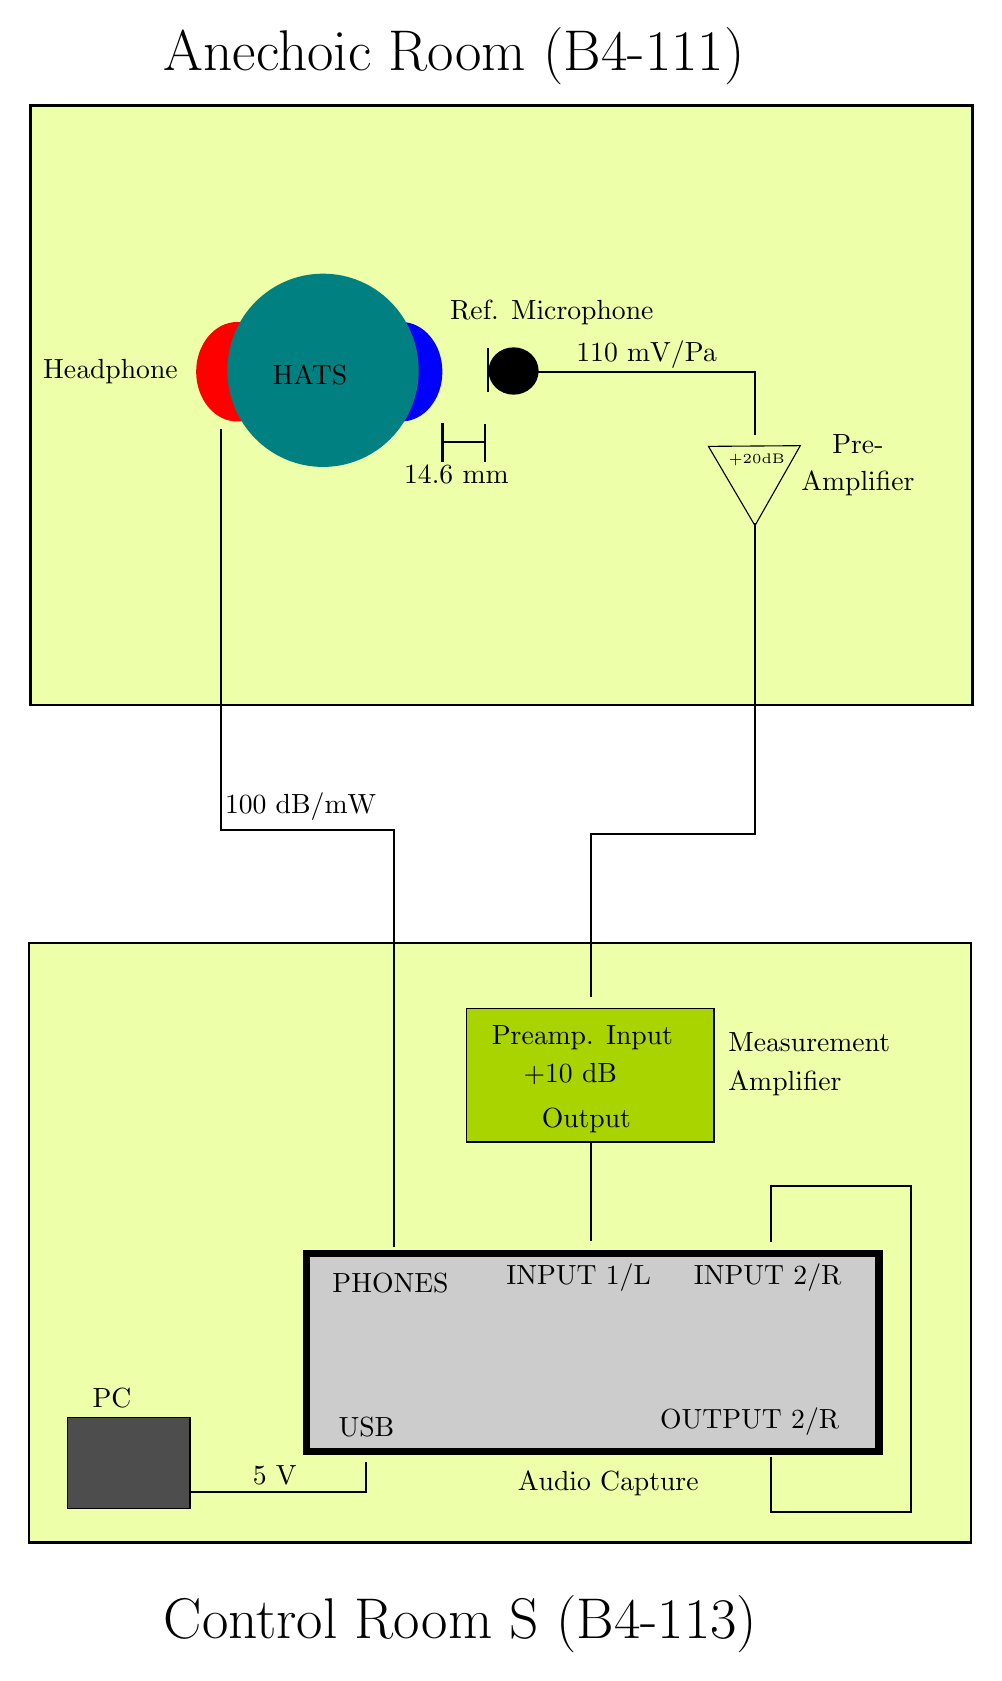
\begin{tikzpicture}[y=0.80pt, x=0.80pt, yscale=-1.000000, xscale=1.000000, inner sep=0pt, outer sep=0pt]
\begin{scope}% layer1
  % rect3342
  \path[draw=black,fill=ceeffaa,line join=miter,line cap=butt,even odd rule,line
    width=0.968pt,rounded corners=0.0000cm] (160.5802,93.3428) rectangle
    (586.0658,364.2491);

  % path3348-0
  \path[fill=c0000ff] (328.0701,213.6738) ellipse (0.5225cm and 0.6318cm);

  % path3348-0-0
  \path[fill=cff0000] (254.0175,213.6738) ellipse (0.5225cm and 0.6318cm);

  % text3399
  \path[fill=black,line join=miter,line cap=butt,line width=0.800pt]
    (220.8386,84.1497) node[above right] (text3399) {\huge{Anechoic Room (B4-111)}};

  % path3415
  \path[draw=black,line join=miter,line cap=butt,even odd rule,line width=0.800pt]
    (367.1652,202.9987) -- (367.1652,222.8035);

  % path3417
  \path[fill=black] (378.8253,213.3426) ellipse (0.3179cm and 0.3007cm);

  % text3425
  \path[fill=black,line join=miter,line cap=butt,line width=0.800pt]
    (407.1953,212.2592) node[above right] (text3425) {110 mV/Pa};

  % path3350-7
  \path[fill=c008080] (292.7422,213.0265) ellipse (1.2151cm and 1.2272cm);

  % path3471
  \path[draw=black,line join=miter,line cap=butt,even odd rule,line width=0.800pt]
    (346.7410,236.9996) -- (346.7410,254.3237);

  % path3471-4
  \path[draw=black,line join=miter,line cap=butt,even odd rule,line width=0.800pt]
    (366.0000,237.2002) -- (366.0000,254.5243);

  % path3488
  \path[draw=black,line join=miter,line cap=butt,even odd rule,line width=0.800pt]
    (347.0127,245.5534) -- (365.8394,245.5534);

  % text3490
  \path[fill=black,line join=miter,line cap=butt,line width=0.800pt]
    (329.3616,264.2414) node[above right] (text3490) {14.6 mm};

  % text3494
  \path[fill=black,line join=miter,line cap=butt,line width=0.800pt]
    (270.0000,219.3622) node[above right] (text3494) {HATS};

  % text3520
  \path[fill=black,line join=miter,line cap=butt,line width=0.800pt]
    (166.3521,219.0369) node[above right] (text3520) {Headphone};

  % text3524
  \path[fill=black,line join=miter,line cap=butt,line width=0.800pt]
    (350.1392,192.5204) node[above right] (text3524) {Ref. Microphone};

  % path3536
  \path[cm={{0.50668,0.86213,-0.86213,0.50668,(553.19003,422.32154)}},draw=black,fill=black,fill
    opacity=0.000] (-153.0817,-14.1755) -- (-194.5745,-14.1755) --
    (-173.8281,-50.1093) -- cycle;

  % path4338
  \path[draw=black,line join=miter,line cap=butt,even odd rule,line width=0.749pt]
    (389.8283,213.8867) -- (487.6847,213.8867) -- (487.6847,242.3189);

  % text4340
  \path[fill=black,line join=miter,line cap=butt,line width=0.800pt]
    (475.9017,256.3146) node[above right] (text4340) {\tiny{+20dB}};

  % text4346
  \path[fill=black,line join=miter,line cap=butt,line width=0.800pt]
    (515.8203,272.6747) node[above right] (text4346) {};

  % text4350
  \path[fill=black,line join=miter,line cap=butt,line width=0.800pt]
  (522.7854,250.5729) node[above right] (text4350) {Pre-};
  
  \path[fill=black,line join=miter,line cap=butt,line width=0.800pt]
    (508.7854,269.5729) node[above right] (text4350) {Amplifier};

  % rect3342-0
  \path[draw=black,fill=ceeffaa,line join=miter,line cap=butt,even odd rule,line
    width=0.968pt,rounded corners=0.0000cm] (159.9447,471.6903) rectangle
    (585.4303,742.5966);

  % text3399-2
  \path[fill=black,line join=miter,line cap=butt,line width=0.800pt]
    (220.8386,792.2573) node[above right] (text3399-2) {\centering{\huge{Control Room S (B4-113)}}};

  % text4387
  \path[fill=black,line join=miter,line cap=butt,line width=0.800pt]
    (285.9375,785.1747) node[above right] (text4387) {};

  % rect4395
  \path[draw=black,fill=ccccccc,line width=2.558pt,rounded corners=0.0000cm]
    (285.0705,611.9925) rectangle (543.8727,701.3781);

  % rect4397
  \path[draw=black,fill=c4d4d4d,line width=0.507pt,rounded corners=0.0000cm]
    (177.3497,685.9109) rectangle (232.6891,727.0794);

  % text4401
  \path[fill=black,line join=miter,line cap=butt,line width=0.800pt]
    (188.6317,681.3109) node[above right] (text4401) {PC};

  % text4405
  \path[fill=black,line join=miter,line cap=butt,line width=0.800pt]
    (380.7714,721.5567) node[above right] (text4405) {Audio Capture};

  % text4409
  \path[fill=black,line join=miter,line cap=butt,line width=0.800pt]
    (299.7695,694.7996) node[above right] (text4409) {USB};

  % path4417
  \path[draw=black,line join=miter,line cap=butt,even odd rule,line width=0.428pt]
    (232.8075,719.6862) -- (312.1120,719.6862) -- (312.1120,705.9801);

  % text5031
  \path[fill=black,line join=miter,line cap=butt,line width=0.800pt]
    (261.0862,716.0892) node[above right] (text5031) {5 V};

  % text5035
  \path[fill=black,line join=miter,line cap=butt,line width=0.800pt]
    (297.0000,629.3622) node[above right] (text5035) {PHONES};

  % path5039
  \path[draw=black,line join=miter,line cap=butt,even odd rule,line width=0.689pt]
    (324.9365,609.1651) -- (324.9365,420.7478) -- (246.6966,420.7478) --
    (246.6966,239.4242);

  % text5315
  \path[fill=black,line join=miter,line cap=butt,line width=0.800pt]
    (248.4749,416.5442) node[above right] (text5315) {100 dB/mW};

  % text5319
  \path[fill=black,line join=miter,line cap=butt,line width=0.800pt]
    (375.5305,629.0000) node[above right] (text5319) {INPUT 1/L};

  % path6749
  \path[draw=black,line join=miter,line cap=butt,even odd rule,line width=0.677pt]
    (487.8216,282.0222) -- (487.8216,422.5549) -- (413.5950,422.5549) --
    (413.5950,496.2119);

  % text5319-3
  \path[fill=black,line join=miter,line cap=butt,line width=0.800pt]
    (460.2651,629.0000) node[above right] (text5319-3) {INPUT 2/R};

  % text7847
  \path[fill=black,line join=miter,line cap=butt,line width=0.800pt]
    (445.0128,693.9413) node[above right] (text7847) {OUTPUT 2/R};

  % path7851
  \path[draw=black,line join=miter,line cap=butt,even odd rule,line width=0.684pt]
    (495.1485,703.8376) -- (495.1485,728.7909) -- (558.3474,728.7909) --
    (558.3474,581.4711) -- (495.1485,581.4711) -- (495.1485,606.8978);

  % rect10551
  \path[draw=black,fill=caad400,rounded corners=0.0000cm] (357.6139,501.4652)
    rectangle (469.3367,561.5693);

  % path10883
  \path[draw=black,line join=miter,line cap=butt,even odd rule,line width=0.716pt]
    (414.0000,561.8622) -- (414.0000,606.1778);

  % text11321
  \path[fill=black,line join=miter,line cap=butt,line width=0.800pt]
    (475.8738,520.7976) node[above right] (text11321) {Measurement};
  
  \path[fill=black,line join=miter,line cap=butt,line width=0.800pt]
    (475.8738,540.7976) node[above right] (text11321) {Amplifier};

  % text11325
  \path[fill=black,line join=miter,line cap=butt,line width=0.800pt]
    (383.3500,535.6852) node[above right] (text11325) {+10 dB};

  % text11329
  \path[fill=black,line join=miter,line cap=butt,line width=0.800pt]
    (368.9959,520.0778) node[above right] (text11329) {Preamp. Input};

  % text11333
  \path[fill=black,line join=miter,line cap=butt,line width=0.800pt]
    (391.5484,557.4692) node[above right] (text11333) {Output};

\end{scope}
\end{tikzpicture}
}

	\caption{Total overview of the test set-up.}
	\label{SchematicOverviewHP}
\end{figure}
%\todoKiis{In the CP experiment the measurement amplifier was in the anechoic - did that change for this experiment?}
\subsection{Settings/Description}
\label{SettingsHeadPhones}
Calibration of the microphone and associated preamplifier is done on the computer using Simulink. The following settings are present:

\subsubsection{Control and calibration}
\begin{itemize}
	\item Microphone sensitivity is controlled to 110 $m$V/Pa.
	\item Measurement amplifier is set to -10 dB default.
	%\item Calibration signal yields an amplitude of 0.87 relative to 0 dBFS. \todoKiis{what is this information? and is it used?}
	\item Calibration signal yields a spike at 101.3 dBSPL $@$ 1 $k$Hz, the expected value is 93.6 dBSPL. Measured values requires a -7.7 dBSPL adjustment.
\end{itemize}
\subsubsection{Equipment settings}
\begin{itemize}
	\item This experiment is performed with a sampling rate of, $f_{s}$ = 48 $k$Hz.
	\item Outside microphone is placed 12.6 mm from headphone cup. 
	\item Settings for the Roland Edirol:
	\begin{itemize}
		\item "SENS(INPUT 1/L)" is set to +0 dB.
		\item "SENS(INPUT 2/R)" is set to +0 dB.
		\item "PHONES" is set to maximum volume. %\todoOliver{again max volume??}
	\end{itemize}		
	\item The measuring amplifier:
		\begin{itemize}
			\item "Input Section Gain" is set to +10 dB.
			% \todoOliver{so +10dB?? Write that }
			\item 22.4 $k$Hz low-pass filter is enabled.
			\item 22.4 Hz high-pass filter is enabled.
			 %\todoOliver{And very little sound is let through. Oliver: okay this doens't make much sense, but recordings are fine}
		\end{itemize}
	\item All gains on the computer is set to 0 dBFS.
\end{itemize}

\subsection{Pictures}
\begin{figure}[H]
	\centering
	\includegraphics[width=0.8\textwidth]{CancellationPath_and_Headphones/CloseUpMicNew.jpg}
	\caption{Full set-up of experiment.}
	\label{CloseupHeadphone}
\end{figure}

%\begin{figure}[H]
%	\centering
%	\includegraphics[width=0.8\textwidth]{CancellationPath_and_Headphones/CloseUpMic.jpg}
%	\caption{Close up of experiment.}
%	\label{CloseUpCancellationPath}
%\end{figure}

\subsection{Procedure}
\subsubsection{Set-up}
\begin{enumerate}
	\item Set instruments to comply with the list in \ref{SettingsHeadPhones}.
	\item Calibrate the microphone using the calibrator.
	\item Place the headphone on the HATS.
	\item Connect the microphone to the preamplifier. 
	\item Connect the preamplifier to the measuring amplifier.
	\item Connect the measuring amplifier to the Roland Edirol. 
	\item Connect the Roland Edirol to the computer via USB.
	\item Connect the headphones to the phones output of the Roland Edirol.
\end{enumerate}

\subsubsection{Performing the experiment}
\begin{enumerate}
	\item Start Simulink and run file  \path{SimulinkSystemHeadPhone.slx}.
	\item The simulation outputs a logarithmic chirp from 20 Hz to 20,000 Hz with an amplitude of 0 dBFS over the span of five seconds.
	\item Record and save, and name "Mic[i].wav" and "Ref[i].wav"\footnote{[i] indicates the iteration of the experiment.}.
\end{enumerate}
Perform this experiment for a total of five times.
If  a drop-out in the recorded signals occurs, then discard that recording and redo the experiment for the current iteration.

\subsection{Data Extraction}
\begin{enumerate}
	%\item Place generated .wav-files in same folder as MATLAB\textsuperscript{\textregistered}-script "HeadPhoneScript.m".
	\item Open Matlab and run script \path{HeadPhoneScript.m}.
\end{enumerate}

From the performing of the experiment, ten files have been generated:
\begin{itemize}
	\item Mic1.wav, Mic2.wav, Mic3.wav, Mic4.wav and Mic5.wav.
	\item Ref1.wav, Ref2.wav, Ref3.wav, Ref4.wav and Ref5.wav.
\end{itemize}

These files are the results of performing the six second simulation which gives a number of 288,768 samples, for each generated .wav-file. 
%\todoOliver{Again - not 6*48000??} Oliver: Same answer as in CP.
The recorded HPMic1 and HPRef1 are shown in \autoref{HeadPhoneAmplitudePlot}.

%\begin{figure}[H]
%	\centering
%	\includegraphics[width=0.85\textwidth]{HeadPhone_MATLAB_Figures/HeadPhoneAmplitudePlot.png}
%	\caption{Amplitude plot of the headphones (NOT TIKZ).}
%	\label{HeadPhoneAmplitudePlot}
%\end{figure}

\begin{figure}[H]
	\centering
	\tikzsetnextfilename{HeadPhoneAmplitudePlot2}
	% This file was created by matlab2tikz.
%
%The latest updates can be retrieved from
%  http://www.mathworks.com/matlabcentral/fileexchange/22022-matlab2tikz-matlab2tikz
%where you can also make suggestions and rate matlab2tikz.
%
\definecolor{mycolor1}{rgb}{0.00000,0.44700,0.74100}%
\definecolor{mycolor2}{rgb}{0.85000,0.32500,0.09800}%
%
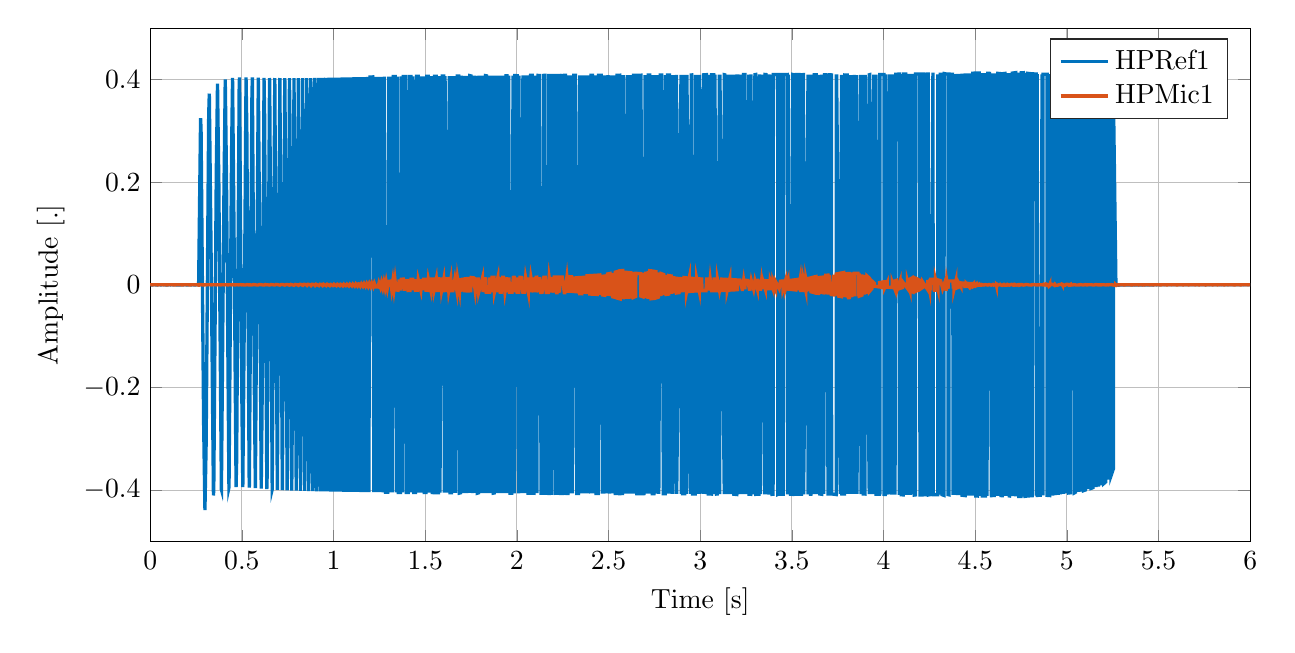
\begin{tikzpicture}

\begin{axis}[%
width=5.5in,
height=2.566in,
at={(0.758in,0.481in)},
scale only axis,
xmin=0,
xmax=6,
xlabel={Time [s]},
xmajorgrids,
ymin=-0.5,
ymax=0.5,
ylabel={Amplitude [.]},
ymajorgrids,
axis background/.style={fill=white},
legend style={legend cell align=left,align=left,draw=white!15!black}
]
\addplot [color=mycolor1,very thick,solid]
  table[row sep=crcr]{%
2.08333333333333e-05	0\\
0.00160416666666667	3.0517578125e-05\\
0.00666666666666667	-9.1552734375e-05\\
0.0148125	-6.103515625e-05\\
0.0263541666666667	6.103515625e-05\\
0.028	3.0517578125e-05\\
0.0290416666666667	-6.103515625e-05\\
0.0421041666666667	-6.103515625e-05\\
0.0474791666666667	6.103515625e-05\\
0.0554791666666667	-6.103515625e-05\\
0.0555833333333333	3.0517578125e-05\\
0.0794791666666667	6.103515625e-05\\
0.0805833333333333	-9.1552734375e-05\\
0.0833125	3.0517578125e-05\\
0.084	-9.1552734375e-05\\
0.09725	-6.103515625e-05\\
0.0977291666666667	6.103515625e-05\\
0.110979166666667	-6.103515625e-05\\
0.111479166666667	3.0517578125e-05\\
0.124833333333333	-6.103515625e-05\\
0.125375	6.103515625e-05\\
0.138833333333333	3.0517578125e-05\\
0.139854166666667	-9.1552734375e-05\\
0.1526875	3.0517578125e-05\\
0.15275	-6.103515625e-05\\
0.166541666666667	-6.103515625e-05\\
0.1766875	6.103515625e-05\\
0.180229166666667	3.0517578125e-05\\
0.180625	-6.103515625e-05\\
0.1950625	6.103515625e-05\\
0.196	-9.1552734375e-05\\
0.208	-6.103515625e-05\\
0.219125	6.103515625e-05\\
0.222895833333333	6.103515625e-05\\
0.223354166666667	-9.1552734375e-05\\
0.236604166666667	6.103515625e-05\\
0.237395833333333	-9.1552734375e-05\\
0.249625	-6.103515625e-05\\
0.256083333333333	6.103515625e-05\\
0.263916666666667	-6.103515625e-05\\
0.274604166666667	0.3248291015625\\
0.277270833333333	0.302764892578125\\
0.291125	-0.2672119140625\\
0.291125	-0.2672119140625\\
0.298375	-0.43878173828125\\
0.304979166666667	-0.308990478515625\\
0.318854166666667	0.331085205078125\\
0.322208333333333	0.372711181640625\\
0.332708333333333	0.03741455078125\\
0.332708333333333	0.03741455078125\\
0.344791666666667	-0.410430908203125\\
0.346583333333333	-0.3988037109375\\
0.3604375	0.2232666015625\\
0.3669375	0.391998291015625\\
0.374291666666667	0.19525146484375\\
0.374291666666667	0.19525146484375\\
0.388145833333333	-0.39886474609375\\
0.3883125	-0.399078369140625\\
0.402020833333333	0.1805419921875\\
0.402020833333333	0.1805419921875\\
0.409166666666667	0.40008544921875\\
0.415875	0.212432861328125\\
0.429291666666667	-0.394927978515625\\
0.42975	-0.3941650390625\\
0.443604166666667	0.257049560546875\\
0.449020833333333	0.403289794921875\\
0.457458333333333	0.08868408203125\\
0.457458333333333	0.08868408203125\\
0.46825	-0.393951416015625\\
0.471333333333333	-0.34320068359375\\
0.4851875	0.388763427734375\\
0.486791666666667	0.404266357421875\\
0.4990625	-0.198883056640625\\
0.504979166666667	-0.394317626953125\\
0.512916666666667	-0.072113037109375\\
0.512916666666667	-0.072113037109375\\
0.522625	0.404266357421875\\
0.526770833333333	0.3067626953125\\
0.539958333333333	-0.3951416015625\\
0.540645833333333	-0.392425537109375\\
0.5545	0.36322021484375\\
0.5569375	0.40399169921875\\
0.568354166666667	-0.221435546875\\
0.5734375	-0.3961181640625\\
0.582229166666667	0.05206298828125\\
0.582229166666667	0.05206298828125\\
0.589520833333333	0.403594970703125\\
0.596083333333333	0.11871337890625\\
0.605354166666667	-0.397125244140625\\
0.6099375	-0.244110107421875\\
0.620791666666667	0.40325927734375\\
0.6238125	0.332000732421875\\
0.635916666666667	-0.397979736328125\\
0.637666666666667	-0.373565673828125\\
0.650708333333333	0.40289306640625\\
0.651541666666667	0.39739990234375\\
0.665270833333333	-0.398681640625\\
0.665395833333333	-0.39849853515625\\
0.67925	0.402099609375\\
0.679458333333333	0.402740478515625\\
0.693125	-0.39825439453125\\
0.6935	-0.399383544921875\\
0.706979166666667	0.402252197265625\\
0.707166666666667	0.402618408203125\\
0.720604166666667	-0.399932861328125\\
0.720833333333333	-0.399322509765625\\
0.733770833333333	0.402496337890625\\
0.734708333333333	0.3934326171875\\
0.746770833333333	-0.400421142578125\\
0.7485625	-0.36358642578125\\
0.7594375	0.402496337890625\\
0.762416666666667	0.301910400390625\\
0.7719375	-0.400848388671875\\
0.776291666666667	-0.187744140625\\
0.78425	0.402587890625\\
0.796354166666667	-0.401123046875\\
0.804	0.169281005859375\\
0.808229166666667	0.402587890625\\
0.817875	-0.3397216796875\\
0.819958333333333	-0.4014892578125\\
0.831479166666667	0.4027099609375\\
0.831729166666667	0.401763916015625\\
0.842833333333333	-0.401702880859375\\
0.845604166666667	-0.28765869140625\\
0.853958333333333	0.40283203125\\
0.8649375	-0.40191650390625\\
0.8733125	0.302520751953125\\
0.875791666666667	0.40289306640625\\
0.886416666666667	-0.402099609375\\
0.8871875	-0.392791748046875\\
0.896958333333333	0.403045654296875\\
0.907291666666667	-0.40228271484375\\
0.914895833333333	0.27691650390625\\
0.917520833333333	0.403106689453125\\
0.927583333333333	-0.402435302734375\\
0.928770833333333	-0.376220703125\\
0.937520833333333	0.40325927734375\\
0.9473125	-0.402557373046875\\
0.956479166666667	0.39788818359375\\
0.956958333333333	0.403411865234375\\
0.966520833333333	-0.4027099609375\\
0.9759375	0.403533935546875\\
0.984208333333333	-0.3792724609375\\
0.985229166666667	-0.40289306640625\\
0.994416666666667	0.403656005859375\\
1.00345833333333	-0.4029541015625\\
1.0119375	0.3980712890625\\
1.01241666666667	0.403778076171875\\
1.02125	-0.403045654296875\\
1.03	0.40386962890625\\
1.0385625	-0.40313720703125\\
1.03966666666667	-0.373687744140625\\
1.04716666666667	0.404052734375\\
1.05554166666667	-0.403411865234375\\
1.063875	0.40423583984375\\
1.072125	-0.403289794921875\\
1.08027083333333	0.40435791015625\\
1.08125	0.37530517578125\\
1.08829166666667	-0.40350341796875\\
1.09629166666667	0.404449462890625\\
1.104125	-0.403533935546875\\
1.11195833333333	0.404541015625\\
1.11966666666667	-0.403656005859375\\
1.12727083333333	0.4046630859375\\
1.13479166666667	-0.403656005859375\\
1.1423125	0.40478515625\\
1.1496875	-0.40374755859375\\
1.15702083333333	0.40478515625\\
1.16427083333333	-0.403839111328125\\
1.16441666666667	-0.40277099609375\\
1.17141666666667	0.4049072265625\\
1.1785	-0.40380859375\\
1.1855625	0.40496826171875\\
1.19252083333333	-0.4039306640625\\
1.1994375	0.405059814453125\\
1.21304166666667	0.405120849609375\\
1.21975	-0.404022216796875\\
1.22639583333333	0.405242919921875\\
1.23297916666667	-0.404083251953125\\
1.2395	0.40533447265625\\
1.24595833333333	-0.404083251953125\\
1.252375	0.40533447265625\\
1.25872916666667	-0.4041748046875\\
1.26502083333333	0.405426025390625\\
1.27129166666667	-0.404205322265625\\
1.27747916666667	0.405517578125\\
1.28360416666667	-0.40423583984375\\
1.29572916666667	-0.404296875\\
1.30170833333333	0.405609130859375\\
1.307625	-0.404296875\\
1.31354166666667	0.40570068359375\\
1.31939583333333	-0.404327392578125\\
1.3251875	0.405731201171875\\
1.336625	0.40582275390625\\
1.34229166666667	-0.404449462890625\\
1.34789583333333	0.405853271484375\\
1.35347916666667	-0.4044189453125\\
1.36447916666667	-0.404449462890625\\
1.36995833333333	0.405975341796875\\
1.37533333333333	-0.40447998046875\\
1.38070833333333	0.406005859375\\
1.3913125	0.406005859375\\
1.39658333333333	-0.404571533203125\\
1.40695833333333	-0.404541015625\\
1.41210416666667	0.406097412109375\\
1.42225	0.406097412109375\\
1.42729166666667	-0.40460205078125\\
1.43229166666667	0.40618896484375\\
1.43725	-0.404632568359375\\
1.4470625	-0.404632568359375\\
1.45191666666667	0.40625\\
1.46154166666667	0.40625\\
1.4663125	-0.404693603515625\\
1.4710625	0.406341552734375\\
1.47577083333333	-0.40472412109375\\
1.4896875	0.4063720703125\\
1.49427083333333	-0.404754638671875\\
1.50335416666667	-0.404754638671875\\
1.50783333333333	0.406402587890625\\
1.51677083333333	0.40643310546875\\
1.52116666666667	-0.40484619140625\\
1.53425	0.406494140625\\
1.5385625	-0.40484619140625\\
1.547125	-0.4049072265625\\
1.55133333333333	0.40655517578125\\
1.55972916666667	0.40655517578125\\
1.56389583333333	-0.40496826171875\\
1.57214583333333	-0.404937744140625\\
1.57625	0.4066162109375\\
1.5803125	-0.404998779296875\\
1.59239583333333	0.406646728515625\\
1.6003125	0.406707763671875\\
1.60425	-0.405120849609375\\
1.60816666666667	0.40673828125\\
1.61979166666667	-0.405120849609375\\
1.63120833333333	0.40679931640625\\
1.635	-0.40521240234375\\
1.64245833333333	-0.4051513671875\\
1.64620833333333	0.4068603515625\\
1.65720833333333	-0.4052734375\\
1.66085416666667	0.4068603515625\\
1.66447916666667	-0.405303955078125\\
1.67522916666667	0.406951904296875\\
1.6823125	0.406951904296875\\
1.68583333333333	-0.405914306640625\\
1.6928125	-0.405303955078125\\
1.69627083333333	0.407562255859375\\
1.7065625	-0.405975341796875\\
1.70995833333333	0.407012939453125\\
1.72670833333333	-0.4058837890625\\
1.73004166666667	0.40704345703125\\
1.73985416666667	-0.405426025390625\\
1.74310416666667	0.407623291015625\\
1.7495625	0.4071044921875\\
1.759125	-0.406036376953125\\
1.76858333333333	0.407623291015625\\
1.7716875	-0.40545654296875\\
1.7748125	0.407135009765625\\
1.78404166666667	-0.406036376953125\\
1.79014583333333	-0.405426025390625\\
1.79316666666667	0.407623291015625\\
1.8021875	-0.406005859375\\
1.81108333333333	0.407623291015625\\
1.819875	-0.406005859375\\
1.8285625	0.4075927734375\\
1.83429166666667	0.407196044921875\\
1.83714583333333	-0.405975341796875\\
1.845625	0.4075927734375\\
1.85402083333333	-0.40594482421875\\
1.8623125	0.40765380859375\\
1.87052083333333	-0.405975341796875\\
1.87591666666667	-0.4056396484375\\
1.87860416666667	0.407684326171875\\
1.886625	-0.405975341796875\\
1.8945625	0.4075927734375\\
1.90239583333333	-0.40594482421875\\
1.91016666666667	0.40765380859375\\
1.91783333333333	-0.405975341796875\\
1.9254375	0.407623291015625\\
1.9329375	-0.405914306640625\\
1.940375	0.407470703125\\
1.94529166666667	0.407440185546875\\
1.94775	-0.40582275390625\\
1.95502083333333	0.407562255859375\\
1.96225	-0.40594482421875\\
1.97175	-0.406005859375\\
1.9788125	0.407501220703125\\
1.98579166666667	-0.40618896484375\\
1.98810416666667	0.407745361328125\\
2.00183333333333	0.407501220703125\\
2.00860416666667	-0.406341552734375\\
2.01083333333333	0.407806396484375\\
2.0219375	-0.405914306640625\\
2.032875	0.408050537109375\\
2.03504166666667	-0.405975341796875\\
2.0415	0.407958984375\\
2.04364583333333	-0.40594482421875\\
2.05847916666667	0.407989501953125\\
2.0605625	-0.405975341796875\\
2.068875	-0.40594482421875\\
2.07504166666667	0.408050537109375\\
2.0831875	0.408050537109375\\
2.08520833333333	-0.405975341796875\\
2.09325	-0.406158447265625\\
2.09920833333333	0.40765380859375\\
2.10904166666667	-0.406036376953125\\
2.114875	0.408050537109375\\
2.12260416666667	0.40802001953125\\
2.132125	-0.406036376953125\\
2.14339583333333	-0.406005859375\\
2.14525	0.408050537109375\\
2.15264583333333	0.4080810546875\\
2.15447916666667	-0.4061279296875\\
2.16902083333333	-0.4063720703125\\
2.17439583333333	0.407745361328125\\
2.17795833333333	0.40777587890625\\
2.18327083333333	-0.406341552734375\\
2.19029166666667	-0.40625\\
2.1955	0.407806396484375\\
2.20925	0.407806396484375\\
2.2109375	-0.40625\\
2.2210625	-0.4061279296875\\
2.2260625	0.407928466796875\\
2.2326875	0.407989501953125\\
2.23433333333333	-0.4063720703125\\
2.25058333333333	-0.406524658203125\\
2.2521875	0.408050537109375\\
2.26489583333333	0.408233642578125\\
2.26647916666667	-0.406341552734375\\
2.2789375	-0.406524658203125\\
2.28047916666667	0.408111572265625\\
2.28814583333333	-0.406494140625\\
2.29575	0.408203125\\
2.30325	-0.40655517578125\\
2.3106875	0.408203125\\
2.3195	0.408203125\\
2.32677083333333	-0.40655517578125\\
2.33539583333333	-0.406524658203125\\
2.3425	0.40814208984375\\
2.34391666666667	-0.406463623046875\\
2.34533333333333	0.407958984375\\
2.35791666666667	-0.406494140625\\
2.35929166666667	0.408111572265625\\
2.37704166666667	-0.40655517578125\\
2.37839583333333	0.40814208984375\\
2.38510416666667	-0.40655517578125\\
2.3864375	0.408172607421875\\
2.40354166666667	-0.4066162109375\\
2.40485416666667	0.408172607421875\\
2.41260416666667	0.408203125\\
2.413875	-0.40655517578125\\
2.43035416666667	0.40826416015625\\
2.43160416666667	-0.406524658203125\\
2.44402083333333	-0.406646728515625\\
2.44525	0.408233642578125\\
2.45983333333333	0.408203125\\
2.46583333333333	-0.40667724609375\\
2.47177083333333	0.408203125\\
2.47295833333333	-0.406768798828125\\
2.48816666666667	0.408172607421875\\
2.4893125	-0.4066162109375\\
2.49735416666667	0.408355712890625\\
2.5053125	-0.406707763671875\\
2.51541666666667	0.40826416015625\\
2.51652083333333	-0.406494140625\\
2.53520833333333	0.4083251953125\\
2.53629166666667	-0.406646728515625\\
2.54489583333333	-0.40667724609375\\
2.54595833333333	0.40826416015625\\
2.56077083333333	0.408477783203125\\
2.5618125	-0.4068603515625\\
2.5763125	-0.406768798828125\\
2.57733333333333	0.408447265625\\
2.57835416666667	-0.40679931640625\\
2.579375	0.40838623046875\\
2.59252083333333	-0.406829833984375\\
2.60147916666667	0.408538818359375\\
2.608375	-0.406768798828125\\
2.61520833333333	0.408447265625\\
2.62389583333333	-0.406829833984375\\
2.62485416666667	0.408538818359375\\
2.6353125	-0.406829833984375\\
2.63625	0.408447265625\\
2.65304166666667	0.408477783203125\\
2.65395833333333	-0.406829833984375\\
2.66672916666667	-0.4068603515625\\
2.667625	0.40838623046875\\
2.67660416666667	0.40850830078125\\
2.68635416666667	-0.406951904296875\\
2.69335416666667	-0.4068603515625\\
2.6994375	0.40863037109375\\
2.70716666666667	-0.406890869140625\\
2.71652083333333	0.408599853515625\\
2.72491666666667	0.40863037109375\\
2.72575	-0.406951904296875\\
2.73320833333333	0.408599853515625\\
2.73895833333333	-0.40704345703125\\
2.74710416666667	-0.40692138671875\\
2.74952083333333	0.408538818359375\\
2.7646875	-0.40692138671875\\
2.76547916666667	0.4085693359375\\
2.77410416666667	-0.407135009765625\\
2.782625	0.408721923828125\\
2.79029166666667	0.4088134765625\\
2.798625	-0.406982421875\\
2.80910416666667	-0.4071044921875\\
2.81133333333333	0.40875244140625\\
2.82089583333333	-0.4071044921875\\
2.821625	0.408782958984375\\
2.83177083333333	0.4088134765625\\
2.83964583333333	-0.40704345703125\\
2.8474375	0.408782958984375\\
2.84814583333333	-0.40716552734375\\
2.858625	0.4088134765625\\
2.86895833333333	-0.407318115234375\\
2.871	0.409027099609375\\
2.8716875	-0.40753173828125\\
2.89514583333333	0.408935546875\\
2.897125	-0.4072265625\\
2.90302083333333	0.40899658203125\\
2.90366666666667	-0.407257080078125\\
2.9153125	-0.4072265625\\
2.91722916666667	0.408843994140625\\
2.9255	-0.407379150390625\\
2.92739583333333	0.4090576171875\\
2.9466875	-0.407379150390625\\
2.95097916666667	0.40887451171875\\
2.95341666666667	0.408966064453125\\
2.95766666666667	-0.407379150390625\\
2.97322916666667	-0.40753173828125\\
2.975	0.4093017578125\\
2.99077083333333	-0.40740966796875\\
2.99135416666667	0.408966064453125\\
2.99422916666667	-0.40740966796875\\
2.99595833333333	0.40899658203125\\
3.01464583333333	-0.40740966796875\\
3.0174375	0.40911865234375\\
3.03395833333333	0.409515380859375\\
3.0345	-0.407867431640625\\
3.04154166666667	0.40911865234375\\
3.04422916666667	-0.4075927734375\\
3.06120833333333	-0.40777587890625\\
3.06172916666667	0.409332275390625\\
3.07316666666667	0.409332275390625\\
3.0736875	-0.407623291015625\\
3.08035416666667	0.409423828125\\
3.08897916666667	-0.407684326171875\\
3.092	-0.4075927734375\\
3.10445833333333	0.409332275390625\\
3.1059375	-0.40765380859375\\
3.10741666666667	0.409393310546875\\
3.131125	-0.40789794921875\\
3.13160416666667	0.409393310546875\\
3.1335	0.40924072265625\\
3.13964583333333	-0.40777587890625\\
3.14666666666667	0.409423828125\\
3.1480625	-0.407806396484375\\
3.16325	0.4095458984375\\
3.16370833333333	-0.407958984375\\
3.182125	0.409423828125\\
3.18345833333333	-0.40802001953125\\
3.19922916666667	-0.40863037109375\\
3.20139583333333	0.409942626953125\\
3.2026875	-0.408416748046875\\
3.20397916666667	0.40985107421875\\
3.21635416666667	-0.40802001953125\\
3.217625	0.40960693359375\\
3.2355625	-0.408050537109375\\
3.23597916666667	0.4097900390625\\
3.24416666666667	0.40966796875\\
3.25266666666667	-0.40802001953125\\
3.26504166666667	0.409637451171875\\
3.26622916666667	-0.40814208984375\\
3.27564583333333	-0.408233642578125\\
3.2768125	0.409942626953125\\
3.28647916666667	-0.408294677734375\\
3.29829166666667	0.409576416015625\\
3.3028125	0.40985107421875\\
3.3031875	-0.40826416015625\\
3.32025	-0.40814208984375\\
3.3228125	0.410064697265625\\
3.32827083333333	-0.4080810546875\\
3.3336875	0.40960693359375\\
3.3518125	-0.408233642578125\\
3.3535625	0.40985107421875\\
3.35914583333333	0.409637451171875\\
3.3601875	-0.408111572265625\\
3.37427083333333	0.41009521484375\\
3.37529166666667	-0.408599853515625\\
3.3830625	0.409759521484375\\
3.39208333333333	-0.40826416015625\\
3.397375	-0.408172607421875\\
3.39902083333333	0.40985107421875\\
3.4223125	0.409881591796875\\
3.42327083333333	-0.40850830078125\\
3.42454166666667	-0.4083251953125\\
3.42991666666667	0.4097900390625\\
3.4380625	0.4097900390625\\
3.438375	-0.408172607421875\\
3.45316666666667	-0.408172607421875\\
3.45408333333333	0.40972900390625\\
3.47510416666667	0.409942626953125\\
3.47658333333333	-0.408355712890625\\
3.481	0.40960693359375\\
3.4929375	-0.408111572265625\\
3.50439583333333	-0.408294677734375\\
3.50525	0.409820556640625\\
3.50808333333333	0.409576416015625\\
3.510625	-0.408050537109375\\
3.52291666666667	-0.4080810546875\\
3.52375	0.409698486328125\\
3.53854166666667	0.409759521484375\\
3.5388125	-0.40814208984375\\
3.55277083333333	-0.408050537109375\\
3.55675	0.409423828125\\
3.56254166666667	0.40960693359375\\
3.56385416666667	-0.408203125\\
3.5883125	0.4095458984375\\
3.5885625	-0.40814208984375\\
3.60135416666667	0.409576416015625\\
3.60160416666667	-0.407989501953125\\
3.60408333333333	-0.407928466796875\\
3.60433333333333	0.40936279296875\\
3.62025	-0.407745361328125\\
3.62145833333333	0.409271240234375\\
3.63202083333333	0.409393310546875\\
3.6336875	-0.40777587890625\\
3.64897916666667	0.4093017578125\\
3.652	-0.407562255859375\\
3.66258333333333	-0.408111572265625\\
3.6628125	0.409637451171875\\
3.67391666666667	-0.407562255859375\\
3.678625	0.4090576171875\\
3.68927083333333	0.409027099609375\\
3.6969375	-0.407562255859375\\
3.70645833333333	-0.40753173828125\\
3.70710416666667	0.40911865234375\\
3.71564583333333	0.409027099609375\\
3.71670833333333	-0.407501220703125\\
3.74170833333333	-0.408660888671875\\
3.74191666666667	0.40997314453125\\
3.7429375	-0.408905029296875\\
3.74395833333333	0.41021728515625\\
3.76508333333333	-0.40740966796875\\
3.77041666666667	0.408966064453125\\
3.77041666666667	0.408966064453125\\
3.7721875	-0.4073486328125\\
3.78695833333333	-0.407440185546875\\
3.7886875	0.408966064453125\\
3.802375	0.408843994140625\\
3.8025625	-0.407318115234375\\
3.81691666666667	0.4088134765625\\
3.81820833333333	-0.40728759765625\\
3.82827083333333	0.4088134765625\\
3.82954166666667	-0.4073486328125\\
3.84016666666667	0.409149169921875\\
3.84141666666667	-0.407562255859375\\
3.853625	0.4088134765625\\
3.8545	-0.407196044921875\\
3.87608333333333	0.409027099609375\\
3.87727083333333	-0.407745361328125\\
3.8895625	0.409088134765625\\
3.88972916666667	-0.407562255859375\\
3.8986875	-0.40771484375\\
3.9005	0.4090576171875\\
3.92172916666667	-0.407684326171875\\
3.92220833333333	0.4093017578125\\
3.9244375	0.409515380859375\\
3.93533333333333	-0.40789794921875\\
3.946375	0.409454345703125\\
3.94991666666667	-0.4080810546875\\
3.95770833333333	0.409637451171875\\
3.95877083333333	-0.408111572265625\\
3.9779375	-0.408172607421875\\
3.97808333333333	0.409576416015625\\
3.97970833333333	-0.408416748046875\\
3.97985416666667	0.4097900390625\\
4.00191666666667	0.40985107421875\\
4.00291666666667	-0.4083251953125\\
4.00860416666667	-0.40838623046875\\
4.01185416666667	0.409942626953125\\
4.02595833333333	-0.4085693359375\\
4.03325	0.41009521484375\\
4.0450625	-0.408660888671875\\
4.0468125	0.4102783203125\\
4.04775	-0.408721923828125\\
4.04895833333333	0.410247802734375\\
4.062625	-0.408935546875\\
4.06616666666667	0.410369873046875\\
4.08527083333333	0.410614013671875\\
4.08641666666667	-0.409088134765625\\
4.092875	0.41064453125\\
4.09627083333333	-0.409088134765625\\
4.10722916666667	-0.409332275390625\\
4.10735416666667	0.410797119140625\\
4.1210625	0.41082763671875\\
4.12239583333333	-0.409332275390625\\
4.13141666666667	0.410919189453125\\
4.13985416666667	-0.409393310546875\\
4.14679166666667	0.4110107421875\\
4.147375	-0.409423828125\\
4.16641666666667	0.410888671875\\
4.16789583333333	-0.409637451171875\\
4.17445833333333	-0.40936279296875\\
4.17502083333333	0.41082763671875\\
4.1963125	0.41070556640625\\
4.19860416666667	-0.409393310546875\\
4.20941666666667	-0.409332275390625\\
4.21016666666667	0.41064453125\\
4.21827083333333	0.410614013671875\\
4.218375	-0.409149169921875\\
4.23389583333333	-0.409088134765625\\
4.234	0.4105224609375\\
4.2436875	0.41064453125\\
4.24583333333333	-0.409393310546875\\
4.25677083333333	-0.40869140625\\
4.26922916666667	0.410369873046875\\
4.269625	0.410369873046875\\
4.27110416666667	-0.40887451171875\\
4.29533333333333	-0.40887451171875\\
4.296	0.41015625\\
4.30272916666667	-0.40899658203125\\
4.30958333333333	0.410125732421875\\
4.3185	0.41021728515625\\
4.31914583333333	-0.40899658203125\\
4.32958333333333	-0.410308837890625\\
4.33058333333333	0.41168212890625\\
4.35116666666667	0.410247802734375\\
4.3523125	-0.408843994140625\\
4.35722916666667	-0.409210205078125\\
4.35766666666667	0.4105224609375\\
4.3763125	0.410430908203125\\
4.37945833333333	-0.409149169921875\\
4.38797916666667	0.410614013671875\\
4.3880625	-0.409454345703125\\
4.4014375	0.410858154296875\\
4.403	-0.409576416015625\\
4.41852083333333	0.4112548828125\\
4.41908333333333	-0.40997314453125\\
4.42810416666667	0.411468505859375\\
4.4285	-0.4100341796875\\
4.44558333333333	-0.4107666015625\\
4.446125	0.411865234375\\
4.46166666666667	-0.41070556640625\\
4.46310416666667	0.412109375\\
4.47025	-0.410980224609375\\
4.4733125	0.412200927734375\\
4.48433333333333	-0.410980224609375\\
4.48616666666667	0.412322998046875\\
4.50052083333333	0.412628173828125\\
4.50345833333333	-0.41143798828125\\
4.5115625	-0.411590576171875\\
4.51191666666667	0.412750244140625\\
4.52202083333333	0.41259765625\\
4.52222916666667	-0.411376953125\\
4.53814583333333	0.412628173828125\\
4.53916666666667	-0.411468505859375\\
4.55558333333333	-0.411407470703125\\
4.55591666666667	0.412506103515625\\
4.5643125	-0.411041259765625\\
4.56883333333333	0.412200927734375\\
4.57779166666667	0.412017822265625\\
4.58810416666667	-0.410919189453125\\
4.5893125	0.4119873046875\\
4.589375	-0.410736083984375\\
4.60370833333333	-0.410614013671875\\
4.60377083333333	0.411773681640625\\
4.62214583333333	-0.411102294921875\\
4.6228125	0.41204833984375\\
4.6378125	0.411529541015625\\
4.640125	-0.41070556640625\\
4.64789583333333	-0.4107666015625\\
4.65691666666667	0.411712646484375\\
4.66279166666667	0.411956787109375\\
4.6685625	-0.411041259765625\\
4.67247916666667	0.41229248046875\\
4.68510416666667	-0.411285400390625\\
4.68677083333333	-0.411376953125\\
4.69158333333333	0.412445068359375\\
4.70214583333333	-0.411956787109375\\
4.70241666666667	0.412506103515625\\
4.72033333333333	0.413421630859375\\
4.72091666666667	-0.412353515625\\
4.73429166666667	0.41339111328125\\
4.7369375	-0.412322998046875\\
4.74966666666667	-0.412353515625\\
4.7509375	0.4132080078125\\
4.761125	0.413330078125\\
4.761375	-0.4124755859375\\
4.77047916666667	0.412811279296875\\
4.7718125	-0.412139892578125\\
4.78520833333333	-0.411468505859375\\
4.78535416666667	0.412139892578125\\
4.79897916666667	0.41156005859375\\
4.80016666666667	-0.4111328125\\
4.8104375	-0.410888671875\\
4.8139375	0.411102294921875\\
4.8326875	0.4107666015625\\
4.83345833333333	-0.410675048828125\\
4.83802083333333	0.41033935546875\\
4.83914583333333	-0.41033935546875\\
4.85383333333333	-0.410003662109375\\
4.86489583333333	0.40985107421875\\
4.86883333333333	-0.410064697265625\\
4.87008333333333	0.41009521484375\\
4.8920625	0.4102783203125\\
4.89210416666667	-0.410247802734375\\
4.90666666666667	-0.41064453125\\
4.90670833333333	0.410491943359375\\
4.9078125	-0.4105224609375\\
4.90785416666667	0.410430908203125\\
4.92702083333333	-0.4105224609375\\
4.92745833333333	0.410400390625\\
4.935375	0.409759521484375\\
4.93572916666667	-0.409820556640625\\
4.950875	0.409423828125\\
4.95214583333333	-0.409271240234375\\
4.9643125	0.408538818359375\\
4.96533333333333	-0.40826416015625\\
4.98039583333333	0.407440185546875\\
4.98154166666667	-0.407562255859375\\
4.99308333333333	0.4066162109375\\
4.99435416666667	-0.40655517578125\\
5.00447916666667	0.405792236328125\\
5.01014583333333	-0.4056396484375\\
5.01945833333333	-0.4052734375\\
5.02229166666667	0.405181884765625\\
5.0390625	0.405426025390625\\
5.0401875	-0.405517578125\\
5.0465625	-0.404266357421875\\
5.04727083333333	0.40435791015625\\
5.06489583333333	-0.403656005859375\\
5.06552083333333	0.40362548828125\\
5.07372916666667	-0.402862548828125\\
5.07454166666667	0.40283203125\\
5.08735416666667	0.401397705078125\\
5.090125	-0.401153564453125\\
5.10141666666667	-0.39971923828125\\
5.1065	0.3992919921875\\
5.11591666666667	-0.39794921875\\
5.11845833333333	0.3978271484375\\
5.13058333333333	0.3966064453125\\
5.131875	-0.3966064453125\\
5.14283333333333	-0.39520263671875\\
5.1458125	0.39508056640625\\
5.15685416666667	0.394256591796875\\
5.15804166666667	-0.39434814453125\\
5.17075	0.392822265625\\
5.1723125	-0.39300537109375\\
5.1855	0.390777587890625\\
5.18558333333333	-0.390777587890625\\
5.19891666666667	0.38812255859375\\
5.20058333333333	-0.38751220703125\\
5.2120625	-0.38397216796875\\
5.21225	0.38427734375\\
5.22589583333333	-0.37945556640625\\
5.22629166666667	0.378875732421875\\
5.240375	0.372283935546875\\
5.24102083333333	-0.371734619140625\\
5.25370833333333	-0.358489990234375\\
5.25429166666667	0.357696533203125\\
5.26747916666667	-0.000640869140625\\
5.27741666666667	-0.00048828125\\
5.28145833333333	-0.000579833984375\\
5.29427083333333	-0.00042724609375\\
5.29552083333333	-0.000518798828125\\
5.307625	-0.0003662109375\\
5.30947916666667	-0.00048828125\\
5.31802083333333	-0.00030517578125\\
5.32308333333333	-0.000396728515625\\
5.33010416666667	-0.000274658203125\\
5.33679166666667	-0.0003662109375\\
5.34420833333333	-0.000213623046875\\
5.35066666666667	-0.00030517578125\\
5.35410416666667	-0.00018310546875\\
5.36489583333333	-0.000274658203125\\
5.37572916666667	-0.0001220703125\\
5.38008333333333	-0.000244140625\\
5.38395833333333	-9.1552734375e-05\\
5.39225	-0.00018310546875\\
5.39445833333333	-6.103515625e-05\\
5.406875	-0.00018310546875\\
5.41666666666667	-3.0517578125e-05\\
5.42052083333333	-3.0517578125e-05\\
5.4225625	-0.000152587890625\\
5.43439583333333	0\\
5.43614583333333	-0.0001220703125\\
5.44795833333333	-9.1552734375e-05\\
5.45714583333333	3.0517578125e-05\\
5.463125	3.0517578125e-05\\
5.46316666666667	-9.1552734375e-05\\
5.47539583333333	-6.103515625e-05\\
5.47914583333333	6.103515625e-05\\
5.48945833333333	-6.103515625e-05\\
5.49275	6.103515625e-05\\
5.50335416666667	-6.103515625e-05\\
5.51379166666667	9.1552734375e-05\\
5.51704166666667	-3.0517578125e-05\\
5.52220833333333	9.1552734375e-05\\
5.53164583333333	-3.0517578125e-05\\
5.53258333333333	9.1552734375e-05\\
5.5450625	9.1552734375e-05\\
5.54745833333333	-3.0517578125e-05\\
5.5595625	-3.0517578125e-05\\
5.55970833333333	9.1552734375e-05\\
5.57247916666667	0\\
5.574625	0.0001220703125\\
5.587	0\\
5.590875	0.0001220703125\\
5.60054166666667	0\\
5.6111875	0.0001220703125\\
5.61420833333333	9.1552734375e-05\\
5.6219375	-3.0517578125e-05\\
5.62795833333333	0\\
5.63145833333333	0.0001220703125\\
5.64335416666667	0.0001220703125\\
5.6491875	-3.0517578125e-05\\
5.65760416666667	0\\
5.66266666666667	0.0001220703125\\
5.67135416666667	0.0001220703125\\
5.67308333333333	-3.0517578125e-05\\
5.68610416666667	0\\
5.69225	0.000152587890625\\
5.697625	0\\
5.70185416666667	0.0001220703125\\
5.71135416666667	0\\
5.71360416666667	0.0001220703125\\
5.72495833333333	0\\
5.734875	0.0001220703125\\
5.73889583333333	0\\
5.7475	0.0001220703125\\
5.75285416666667	0\\
5.75302083333333	9.1552734375e-05\\
5.77308333333333	0.0001220703125\\
5.77639583333333	-3.0517578125e-05\\
5.781	0.0001220703125\\
5.78125	0\\
5.7969375	0\\
5.80335416666667	0.0001220703125\\
5.8178125	0.0001220703125\\
5.81966666666667	-3.0517578125e-05\\
5.82264583333333	-3.0517578125e-05\\
5.82410416666667	0.0001220703125\\
5.83627083333333	9.1552734375e-05\\
5.83635416666667	0\\
5.84970833333333	9.1552734375e-05\\
5.84975	0\\
5.864125	9.1552734375e-05\\
5.8665	-3.0517578125e-05\\
5.87739583333333	9.1552734375e-05\\
5.87797916666667	-3.0517578125e-05\\
5.89241666666667	9.1552734375e-05\\
5.89816666666667	-3.0517578125e-05\\
5.90664583333333	9.1552734375e-05\\
5.90789583333333	-3.0517578125e-05\\
5.92160416666667	-3.0517578125e-05\\
5.92725	0.0001220703125\\
5.93420833333333	9.1552734375e-05\\
5.935625	-3.0517578125e-05\\
5.94941666666667	-3.0517578125e-05\\
5.9554375	0.0001220703125\\
5.96097916666667	-3.0517578125e-05\\
5.962875	9.1552734375e-05\\
5.9745625	9.1552734375e-05\\
5.97758333333333	-3.0517578125e-05\\
5.98854166666667	9.1552734375e-05\\
5.99022916666667	-3.0517578125e-05\\
6.016	3.0517578125e-05\\
};
\addlegendentry{HPRef1};

\addplot [color=mycolor2,very thick,solid]
  table[row sep=crcr]{%
2.08333333333333e-05	-2.51524364683429e-06\\
0.00439583333333333	2.64100582917601e-05\\
0.0103541666666667	-8.30030403455316e-05\\
0.0139583333333333	-2.38948146449258e-05\\
0.0245625	0.00010564023316704\\
0.0281041666666667	4.90472511132687e-05\\
0.0402291666666667	-6.28810911708573e-05\\
0.0426041666666667	-6.0365847524023e-05\\
0.055	5.40777384069373e-05\\
0.0644583333333333	7.92301748752802e-05\\
0.0692083333333333	-2.76676801151772e-05\\
0.0721458333333333	-6.41387129942744e-05\\
0.0745208333333333	-2.51524364683429e-06\\
0.0845416666666667	1.50914618810057e-05\\
0.0899583333333333	-9.43216367562859e-05\\
0.09775	-8.80335276392002e-06\\
0.105833333333333	0.000101867367696789\\
0.1140625	5.91082257006058e-05\\
0.1220625	-4.90472511132687e-05\\
0.125208333333333	1.00609745873372e-05\\
0.1315625	-9.68368804031202e-05\\
0.138895833333333	-3.14405455854286e-05\\
0.1451875	0.000100609745873372\\
0.155583333333333	5.1562494760103e-05\\
0.162520833333333	-1.760670552784e-05\\
0.166395833333333	0\\
0.172020833333333	-0.000129535047811966\\
0.1803125	-4.02438983493487e-05\\
0.194041666666667	6.41387129942744e-05\\
0.19625	0.000106897854990457\\
0.207729166666667	-2.51524364683429e-06\\
0.208	6.28810911708573e-06\\
0.212083333333333	-0.000108155476813875\\
0.222083333333333	-5.40777384069373e-05\\
0.235541666666667	4.90472511132687e-05\\
0.2356875	4.77896292898515e-05\\
0.249020833333333	-4.15015201727658e-05\\
0.24975	-4.65320074664344e-05\\
0.256229166666667	4.27591419961829e-05\\
0.265229166666667	-0.000646417617236413\\
0.268020833333333	0.00070929870840727\\
0.278979166666667	0.000259070095623932\\
0.284270833333333	-0.000137080778752469\\
0.2959375	-8.6775905815783e-05\\
0.301895833333333	8.17454185221145e-05\\
0.3065625	-0.000133307913282217\\
0.311708333333333	5.03048729366858e-05\\
0.32425	0.000215053331804332\\
0.3320625	-0.000173551811631566\\
0.33275	-0.000174809433454983\\
0.3450625	8.30030403455316e-05\\
0.3475	8.80335276392002e-05\\
0.360354166666667	-8.80335276392002e-05\\
0.362104166666667	-0.000134565535105635\\
0.3685625	0.000186128029865738\\
0.374395833333333	7.04268221113601e-05\\
0.379645833333333	-0.000155945106103726\\
0.388208333333333	-5.53353602303544e-05\\
0.394	9.43216367562859e-05\\
0.404791666666667	-0.000101867367696789\\
0.4144375	0.000287995397562526\\
0.415916666666667	0.000213795709980915\\
0.420770833333333	-0.000178582298925235\\
0.435104166666667	8.30030403455316e-05\\
0.4430625	-0.000106897854990457\\
0.4453125	-0.00011444358593096\\
0.454395833333333	0.000320693564971372\\
0.457458333333333	4.90472511132687e-05\\
0.460166666666667	-0.00014085364422272\\
0.474395833333333	3.77286547025144e-05\\
0.483604166666667	-0.000179839920748652\\
0.492979166666667	0.000347103623263132\\
0.498166666666667	-0.000134565535105635\\
0.5045	1.38338400575886e-05\\
0.512520833333333	-0.000172294189808149\\
0.520354166666667	-0.000265358204741018\\
0.52675	0.000432621907255498\\
0.528083333333333	0.000479153914721932\\
0.534	-7.41996875816116e-05\\
0.540666666666667	-3.52134110556801e-05\\
0.554291666666667	-0.000271646313858103\\
0.554729166666667	-0.000299313993973281\\
0.563458333333333	0.000564672198714298\\
0.5733125	0.000103124989520206\\
0.580791666666667	-0.000320693564971372\\
0.588291666666667	-0.000425076176314995\\
0.595916666666667	0.000661509079117418\\
0.596125	0.000662766700940836\\
0.6099375	-9.43216367562859e-05\\
0.619875	-0.000474123427428264\\
0.6238125	7.41996875816116e-05\\
0.6274375	0.000681631028292093\\
0.632479166666667	-6.28810911708573e-06\\
0.637916666666667	0.000210022844510663\\
0.650270833333333	-0.000538262140422538\\
0.651541666666667	-0.000470350561958012\\
0.657291666666667	0.000614977071650984\\
0.667541666666667	0.000232660037332172\\
0.679104166666667	-0.000503048729366858\\
0.679770833333333	-0.00048041153654535\\
0.686270833333333	0.000710556330230687\\
0.695666666666667	0.000275419179328355\\
0.70675	-0.000675342919175007\\
0.707145833333333	-0.000686661515585761\\
0.714270833333333	0.000643902373589578\\
0.723854166666667	0.000369740816084641\\
0.733770833333333	-0.000642644751766161\\
0.734791666666667	-0.000581021282418721\\
0.740520833333333	0.00057724841694847\\
0.75225	0.000303086859443532\\
0.75925	-0.000758345959520539\\
0.762416666666667	-0.000270388692034686\\
0.766145833333333	0.000818711807044562\\
0.7845	-0.000968368804031202\\
0.790145833333333	0.000518140191247864\\
0.791125	0.000777210286871796\\
0.804	-9.05487712860345e-05\\
0.808854166666667	-0.00111425293554759\\
0.8156875	0.000957050207620448\\
0.825625	0.00072690541393511\\
0.831729166666667	-0.00120983219412729\\
0.832395833333333	-0.00127397090712157\\
0.838458333333333	0.000934413014798939\\
0.848479166666667	0.000711813952054104\\
0.855354166666667	-0.00137709589664177\\
0.86175	0.00102747702973181\\
0.8733125	3.64710328790972e-05\\
0.877604166666667	-0.00146764466792781\\
0.883854166666667	0.00112557153195835\\
0.892125	0.000694207246526264\\
0.8991875	-0.00164874221049988\\
0.901041666666667	-0.00106520568443432\\
0.905104166666667	0.00112054104466468\\
0.919625	-0.00162610501767837\\
0.9256875	0.00119096786677604\\
0.93325	0.000817454185221145\\
0.940166666666667	-0.00167766751243847\\
0.942625	-0.000822484672514813\\
0.945916666666667	0.00112054104466468\\
0.959645833333333	-0.00171413854531757\\
0.965541666666667	0.00116204256483744\\
0.97875	-0.00170659281437707\\
0.984166666666667	0.00105137184437673\\
0.984354166666667	0.00106772092808116\\
0.997583333333333	-0.00172042665443465\\
0.998145833333333	-0.00162736263950179\\
1.00291666666667	0.00114066299383935\\
1.0154375	-0.00182480926577828\\
1.02110416666667	0.00113814775019252\\
1.03316666666667	-0.00181349066936752\\
1.03860416666667	0.00125384895794689\\
1.03966666666667	0.00117084591760136\\
1.050125	-0.00200464918652693\\
1.05604166666667	0.00132804864552851\\
1.067125	-0.00208262173957879\\
1.067375	-0.00206501503405095\\
1.07339583333333	0.00131924529276459\\
1.08314583333333	-0.00210903179787055\\
1.08947916666667	0.0014374617441658\\
1.09966666666667	-0.00219958056915659\\
1.1054375	0.00149405472621957\\
1.11514583333333	-0.00234420707884956\\
1.12114583333333	0.00171413854531757\\
1.13039583333333	-0.00246242353025077\\
1.13666666666667	0.00190278181883014\\
1.1366875	0.00190278181883014\\
1.1454375	-0.00273406984410887\\
1.15170833333333	0.00198955772464592\\
1.16020833333333	-0.00281078477533732\\
1.16675	0.00215053331804332\\
1.17470833333333	-0.00296421463779421\\
1.180875	0.00232785799514514\\
1.18883333333333	-0.00328742344641242\\
1.19495833333333	0.00257560949435831\\
1.2026875	-0.003506249643687\\
1.2086875	0.00271269027311078\\
1.216375	-0.0036307542042053\\
1.22227083333333	0.00296169939414738\\
1.2296875	-0.00410362000981015\\
1.24270833333333	-0.00438406967643217\\
1.24758333333333	0.0035427206765661\\
1.25572916666667	-0.00483555591103892\\
1.26141666666667	0.00446455747313087\\
1.268375	-0.0056995421037265\\
1.27445833333333	0.00516505282877422\\
1.28095833333333	-0.00625038046238321\\
1.28691666666667	0.00590327683912008\\
1.29314583333333	-0.0069169200287943\\
1.2993125	0.0066012569511166\\
1.31147916666667	0.00731684376864095\\
1.31689583333333	-0.00828521257267215\\
1.323375	0.00816951136491778\\
1.32914583333333	-0.00935670636622356\\
1.33510416666667	0.00913410730347873\\
1.34070833333333	-0.00993772764864228\\
1.35210416666667	-0.0106004943495831\\
1.35791666666667	0.010389213883249\\
1.36329166666667	-0.0111224074063012\\
1.3690625	0.0107652428084508\\
1.37997916666667	0.0111475598427696\\
1.38522916666667	-0.0113362031162821\\
1.39070833333333	0.0111651665482974\\
1.39583333333333	-0.0111978647157063\\
1.40129166666667	0.0111148616753607\\
1.40639583333333	-0.0111727122792379\\
1.41677083333333	-0.0110004180894298\\
1.422	0.0109400522419057\\
1.432125	0.0109475979728463\\
1.4369375	-0.0107161955573375\\
1.44208333333333	0.0109526284601399\\
1.446875	-0.01075392421204\\
1.45666666666667	-0.010648283978873\\
1.46164583333333	0.0107576970775103\\
1.47585416666667	-0.0104810202763585\\
1.48066666666667	0.0107891376230957\\
1.48516666666667	-0.0104395187561857\\
1.48997916666667	0.0107363175065122\\
1.49920833333333	0.010838184874209\\
1.50364583333333	-0.0106193586769344\\
1.51264583333333	-0.0107677580520976\\
1.51720833333333	0.0109765232747848\\
1.53033333333333	-0.0107526665902166\\
1.5348125	0.0111953494720594\\
1.54341666666667	0.0111349836245354\\
1.54770833333333	-0.0110306010131918\\
1.5604375	0.0112532000759366\\
1.56460416666667	-0.0110544958278367\\
1.572875	-0.0109941299803127\\
1.57702083333333	0.0115512564480865\\
1.5851875	0.0114468738367429\\
1.58920833333333	-0.0111802580101784\\
1.60120833333333	0.0114041146947467\\
1.60520833333333	-0.0112670339159942\\
1.61302083333333	-0.0112016375811765\\
1.61685416666667	0.0116682152776643\\
1.6245625	0.0116820491177219\\
1.62839583333333	-0.0113487793345163\\
1.63975	0.0116895948486624\\
1.64347916666667	-0.0114305247530384\\
1.65091666666667	-0.011558802179027\\
1.66189583333333	0.0119247701296414\\
1.67272916666667	-0.0117927198381826\\
1.67633333333333	0.0122580399128469\\
1.68697916666667	-0.0124014088007165\\
1.69039583333333	0.0126956923073961\\
1.70085416666667	-0.0131987410367629\\
1.70425	0.0137621556136538\\
1.71460416666667	-0.0142413095283758\\
1.7179375	0.0147192058212743\\
1.7280625	-0.0149531234804299\\
1.731375	0.0151430243757658\\
1.73472916666667	-0.0149594115895469\\
1.73802083333333	0.0150876890155355\\
1.7478125	-0.0143846784162453\\
1.75104166666667	0.0142614314775504\\
1.76375	0.0136338781876653\\
1.77316666666667	-0.013660288245957\\
1.7824375	0.0144022851217732\\
1.78552083333333	-0.0143368887869555\\
1.78860416666667	0.0145544573624066\\
1.79170833333333	-0.0145469116314661\\
1.81266666666667	0.0141205778333277\\
1.81560416666667	-0.0141671098407941\\
1.824375	0.0146286570499882\\
1.82727083333333	-0.0144563628601801\\
1.83014583333333	0.0144525899947098\\
1.8330625	-0.0143620412234238\\
1.85008333333333	-0.0145343354132319\\
1.85285416666667	0.0144525899947098\\
1.86122916666667	-0.0143456921397194\\
1.8639375	0.0144890610275889\\
1.87485416666667	0.0145003796239997\\
1.87760416666667	-0.0145431387659959\\
1.89622916666667	0.014570806446111\\
1.89889583333333	-0.014540623522349\\
1.90145833333333	0.0145896707734623\\
1.90927083333333	-0.0145217591949978\\
1.9144375	-0.0145695488242876\\
1.92208333333333	0.0145217591949978\\
1.92710416666667	0.0145066677331168\\
1.93466666666667	-0.0145620030933471\\
1.947	0.0145355930350554\\
1.94945833333333	-0.0145242744386446\\
1.95672916666667	0.0144940915148826\\
1.95916666666667	-0.0144701967002377\\
1.97347916666667	-0.0146135655881072\\
1.98052083333333	0.0144966067585294\\
1.9851875	0.0145695488242876\\
1.992125	-0.014570806446111\\
1.999	0.0144475595074162\\
2.00127083333333	-0.0146211113190477\\
2.01033333333333	-0.0145695488242876\\
2.017	0.0144878034057655\\
2.02583333333333	0.0144249223145947\\
2.03241666666667	-0.0145758369334047\\
2.04108333333333	-0.014564518336994\\
2.04747916666667	0.014389708903539\\
2.06229166666667	-0.0146148232099306\\
2.06433333333333	0.0144110884745371\\
2.07058333333333	-0.0146273994281648\\
2.07670833333333	0.014465166212944\\
2.09095833333333	-0.0145670335806408\\
2.09289583333333	0.0145959588825794\\
2.0989375	-0.0145469116314661\\
2.10483333333333	0.0148839542801419\\
2.10875	0.0149078490947868\\
2.11852083333333	-0.0146336875372819\\
2.12427083333333	0.0147858597779154\\
2.13002083333333	-0.0147204634430977\\
2.1375625	-0.0146525518646332\\
2.14689583333333	0.0148047241052666\\
2.15429166666667	0.0147531616105065\\
2.15979166666667	-0.0147242363085679\\
2.17066666666667	-0.0148160427016774\\
2.17602083333333	0.0148323917853818\\
2.18841666666667	-0.0148915000110824\\
2.19016666666667	0.0150160045716007\\
2.2023125	-0.015125417670238\\
2.20402083333333	0.0151317057793551\\
2.21425	0.0152474069871095\\
2.2159375	-0.0153039999691632\\
2.2193125	-0.015390775874979\\
2.22433333333333	0.0152951966163993\\
2.23264583333333	-0.0152863932636354\\
2.23429166666667	0.0152662713144607\\
2.24733333333333	0.015209678332407\\
2.2585625	-0.0152964542382227\\
2.26172916666667	-0.0153203490528677\\
2.27272916666667	0.0152574679616968\\
2.2805	-0.0153844877658619\\
2.28510416666667	0.0154574298316201\\
2.29725	0.0156674526761308\\
2.29879166666667	-0.0156624221888371\\
2.3121875	0.0159881462411022\\
2.31366666666667	-0.0161755318927913\\
2.32683333333333	0.016696187327686\\
2.32827083333333	-0.0166672620257474\\
2.34114583333333	0.0171023991766498\\
2.34258333333333	-0.0172772086101047\\
2.35383333333333	-0.0174683671272641\\
2.35522916666667	0.0174796857236749\\
2.36216666666667	-0.0175878412004888\\
2.36629166666667	0.0175979021750761\\
2.38122916666667	-0.0177312100883583\\
2.3825625	0.0177161186264773\\
2.39585416666667	0.0178544570270532\\
2.39716666666667	-0.0179839920748652\\
2.4101875	-0.0181512557773797\\
2.41147916666667	0.0181952725411993\\
2.42425	0.0184669188550574\\
2.4255	-0.0184543426368232\\
2.43802083333333	-0.0188127648564971\\
2.43927083333333	0.01880647674738\\
2.4515625	0.019171187076171\\
2.45277083333333	-0.019261735847457\\
2.46604166666667	0.0197358592748853\\
2.46722916666667	-0.019747177871296\\
2.4790625	-0.0203332296410084\\
2.48022916666667	0.0203583820774767\\
2.493	-0.0212173377828707\\
2.49416666666667	0.0211720633972276\\
2.5078125	0.0221240831175544\\
2.5089375	-0.022047368186326\\
2.52122916666667	0.0229893269320654\\
2.52233333333333	-0.0233477491517393\\
2.5355	-0.0245701575641008\\
2.53658333333333	0.024673282553621\\
2.54947916666667	0.0261585339270766\\
2.55054166666667	-0.0262704622693608\\
2.56320833333333	-0.0275092197654266\\
2.56425	0.0275356298237184\\
2.5766875	0.0278877639342752\\
2.57770833333333	-0.0279556755127397\\
2.57875	0.0278512929013961\\
2.57977083333333	-0.0279808279492081\\
2.5929375	0.0275620398820102\\
2.5939375	-0.0273834575830849\\
2.60685416666667	0.0270363539598218\\
2.60785416666667	-0.027055218287173\\
2.62052083333333	0.0264830003575182\\
2.62147916666667	-0.0265483966923359\\
2.63391666666667	0.0250317047732949\\
2.634875	-0.0247575432157899\\
2.648	-0.0226019794104529\\
2.6489375	0.0224108208932935\\
2.67441666666667	0.0218109352835236\\
2.6753125	-0.0218436334509324\\
2.68770833333333	-0.0233967964028526\\
2.68858333333333	0.0235414229125455\\
2.70166666666667	-0.0256014074593028\\
2.70252083333333	0.0256668037941205\\
2.71535416666667	-0.0271885262004553\\
2.71620833333333	0.0272715292408008\\
2.72379166666667	-0.0274790368416646\\
2.724625	0.0274513691615495\\
2.73129166666667	0.0272312853424515\\
2.732125	-0.027169661873104\\
2.74525	-0.0265798372379214\\
2.7460625	0.0264628784083436\\
2.75895833333333	0.0256668037941205\\
2.75975	-0.0254982824697826\\
2.77239583333333	-0.0240394411546187\\
2.77316666666667	0.0239174518377473\\
2.78635416666667	-0.022023473371681\\
2.787125	0.0218826197274583\\
2.80079166666667	0.0200930238727357\\
2.80154166666667	-0.0201131458219104\\
2.8141875	0.0190014081300097\\
2.8149375	-0.0187750362017946\\
2.82808333333333	-0.018100950904443\\
2.8288125	0.0179802192093949\\
2.84172916666667	0.0172382223335788\\
2.8424375	-0.0172860119628687\\
2.85579166666667	0.0166446248329259\\
2.8565	-0.0163842971154786\\
2.86960416666667	0.0158435197314092\\
2.87029166666667	-0.0159265227717547\\
2.88383333333333	-0.0152951966163993\\
2.8845	0.0152901661291057\\
2.897125	-0.0146865076538654\\
2.89777083333333	0.0146814771665718\\
2.91145833333333	-0.0141256083206214\\
2.91210416666667	0.0141419574043258\\
2.924875	0.0135621937437305\\
2.92552083333333	-0.0135433294163792\\
2.93991666666667	0.0129006846646131\\
2.94054166666667	-0.013000036788663\\
2.95283333333333	-0.0124957304374728\\
2.95466666666667	0.0126818584673385\\
2.96672916666667	0.0121272472432115\\
2.9673125	-0.0122027045526166\\
2.98033333333333	-0.0119109362895838\\
2.98091666666667	0.0117009134450731\\
2.99427083333333	-0.0114556771895068\\
2.99485416666667	0.0116606695467238\\
3.00852083333333	0.0112569729414069\\
3.00908333333333	-0.011278352512405\\
3.03129166666667	-0.0112708067814645\\
3.03510416666667	0.0112896711088157\\
3.04697916666667	0.011383992745572\\
3.04858333333333	-0.0113123083016372\\
3.0544375	0.0114091451820403\\
3.06233333333333	-0.0113940537201593\\
3.069625	-0.0114342976185087\\
3.0753125	0.0113927960983359\\
3.07839583333333	0.0114015994510998\\
3.08095833333333	-0.0113399759817524\\
3.09210416666667	-0.0112833829996986\\
3.09360416666667	0.0112858982433455\\
3.1050625	-0.0111286955154183\\
3.11633333333333	0.0111110888098905\\
3.11925	0.0110456924750728\\
3.12166666666667	-0.010958916569257\\
3.13316666666667	-0.0107639851866273\\
3.13458333333333	0.0107891376230957\\
3.1468125	0.0105250370401781\\
3.14727083333333	-0.0105690538039977\\
3.16066666666667	0.0103992748578364\\
3.161125	-0.0103187870611377\\
3.17470833333333	-0.0100748084273948\\
3.17514583333333	0.0101112794602738\\
3.18847916666667	0.00972770480413162\\
3.18891666666667	-0.00980316211353665\\
3.20285416666667	-0.00938311642451532\\
3.20329166666667	0.00948498379221211\\
3.21695833333333	0.00927244570405461\\
3.229125	-0.00909134816148254\\
3.22995833333333	-0.00908506005236546\\
3.23697916666667	0.00885994574597379\\
3.2439375	-0.00863105857411187\\
3.24435416666667	0.00880083752027318\\
3.258875	0.00852416071912141\\
3.268	-0.00849146255171257\\
3.27191666666667	-0.00842858146054171\\
3.2785625	0.00849775066082965\\
3.29127083333333	-0.00855057077741317\\
3.2985	0.00857572321388152\\
3.31160416666667	-0.00867256009428464\\
3.31270833333333	0.00865746863240363\\
3.3149375	0.0087140616144574\\
3.3263125	-0.00869645490892956\\
3.32920833333333	-0.00873544118545549\\
3.334625	0.00863986192687579\\
3.34070833333333	-0.00843864243512905\\
3.3410625	0.00854805553376634\\
3.35483333333333	-0.00814813179391968\\
3.3551875	0.00825377202708672\\
3.36904166666667	0.00782115011983123\\
3.369375	-0.00776707238142429\\
3.38229166666667	-0.00748662271480227\\
3.382625	0.00757088337697122\\
3.39629166666667	-0.00717599012441823\\
3.396625	0.00727156938299793\\
3.41002083333333	-0.00708292610948536\\
3.41035416666667	0.00691566240697088\\
3.43045833333333	-0.00711310903324737\\
3.43766666666667	0.0070414245893126\\
3.45064583333333	0.00740236205263332\\
3.4515625	-0.00755327667144338\\
3.46460416666667	0.00794439705852611\\
3.46489583333333	-0.0079808680914052\\
3.47829166666667	0.00846756773706764\\
3.4791875	-0.00842480859507146\\
3.49260416666667	-0.00884736952773962\\
3.49289583333333	0.00877945794927509\\
3.5060625	0.00932400819881472\\
3.50691666666667	-0.00944096702839251\\
3.52039583333333	-0.0100270187981049\\
3.52066666666667	0.00999432063069606\\
3.53445833333333	0.0106357077606388\\
3.53472916666667	-0.0106319348951685\\
3.54475	0.0108155476813875\\
3.54770833333333	-0.0109249607800247\\
3.56097916666667	-0.0109840690057253\\
3.56229166666667	0.0111173769190076\\
3.57608333333333	-0.011528619255265\\
3.57633333333333	0.0116430628411959\\
3.58985416666667	-0.0126177197543442\\
3.59010416666667	0.0123988935570696\\
3.603625	0.0135898614238457\\
3.603875	-0.0135936342893159\\
3.61714583333333	-0.0148424527599692\\
3.617875	0.0150260655461881\\
3.631375	0.0161063626925034\\
3.631625	-0.016225836765728\\
3.64533333333333	-0.0166433672111025\\
3.6455625	0.0166333062365152\\
3.65879166666667	-0.0176507222916596\\
3.65947916666667	0.0177048000300666\\
3.67245833333333	-0.0182480926577828\\
3.6726875	0.0181059813917366\\
3.681875	-0.0186492740194528\\
3.68520833333333	0.0186190910956908\\
3.69708333333333	0.0189033136277831\\
3.69904166666667	-0.0188115072346737\\
3.70489583333333	0.0189146322241939\\
3.71495833333333	-0.0189448151479559\\
3.72845833333333	-0.0196239309326011\\
3.72866666666667	0.0196138699580138\\
3.74210416666667	-0.0211569719353466\\
3.7423125	0.0212009886991662\\
3.75570833333333	0.0221693575031974\\
3.7563125	-0.022213374267017\\
3.76985416666667	-0.0231037705179964\\
3.77004166666667	0.0230773604597046\\
3.78333333333333	0.0240017124999162\\
3.78391666666667	-0.0239878786598586\\
3.79714583333333	0.0246669944445039\\
3.79733333333333	-0.0246091438406267\\
3.80770833333333	0.0250945858644657\\
3.80827083333333	-0.0250933282426423\\
3.812	-0.0249914608749455\\
3.8121875	0.0249210340528342\\
3.826375	-0.0241249594386111\\
3.8265625	0.0242167658317206\\
3.83975	-0.0225340678319884\\
3.84029166666667	0.0223844108350018\\
3.8600625	0.0223693193731208\\
3.86058333333333	-0.0223705769949442\\
3.8676875	0.0220712630009709\\
3.86785416666667	-0.022023473371681\\
3.88185416666667	-0.0202187860550774\\
3.88202083333333	0.020126979661968\\
3.89525	-0.0189586489880135\\
3.89541666666667	0.0189334965515451\\
3.909375	-0.0173325439703351\\
3.90954166666667	0.0173350592139819\\
3.92308333333333	0.0129975215450162\\
3.92325	-0.0130138706287206\\
3.93685416666667	-0.00720491542635683\\
3.937	0.00725647792111693\\
3.950625	0.00280323904439682\\
3.95079166666667	-0.00278060185157531\\
3.97754166666667	-0.00418410780650884\\
3.97829166666667	0.00430358187973347\\
3.99204166666667	0.00531722506940769\\
3.9921875	-0.00544676011721966\\
4.00141666666667	-0.00580140947142329\\
4.00527083333333	0.00579637898412962\\
4.006125	0.00579260611865937\\
4.00627083333333	-0.00572469454019485\\
4.0199375	0.00470476324140354\\
4.02035416666667	-0.00455259100077007\\
4.04741666666667	-0.00535998421140387\\
4.0475625	0.00537130280781463\\
4.061	-0.00751932088221111\\
4.06139583333333	0.00763879495543574\\
4.06952083333333	0.00862477046499478\\
4.07095833333333	-0.00858829943211569\\
4.0755	0.00846631011524422\\
4.075625	-0.0083543817729601\\
4.08958333333333	0.00697728587631832\\
4.08970833333333	-0.00714958006612647\\
4.10327083333333	-0.00552599029209494\\
4.104625	0.00557503754320821\\
4.1305625	-0.00709550232771953\\
4.1306875	0.00700369593461008\\
4.1445625	-0.0112720644032879\\
4.1446875	0.011284640621522\\
4.15772916666667	0.0137998842683563\\
4.15854166666667	-0.0137558675045367\\
4.15945833333333	-0.0139306769379917\\
4.1639375	0.0140086494910436\\
4.17258333333333	0.0131647852475307\\
4.173375	-0.0130415383088358\\
4.18635416666667	-0.0108960354780861\\
4.1866875	0.0108671101761476\\
4.2003125	0.00824999916161647\\
4.20041666666667	-0.00840091378042653\\
4.21441666666667	-0.00501791107543441\\
4.21452083333333	0.00509965649395652\\
4.2411875	-0.00963338316737533\\
4.24129166666667	0.00946360422121402\\
4.25160416666667	-0.0108432153615026\\
4.25372916666667	0.0109211879145545\\
4.25564583333333	-0.0107199684228077\\
4.25575	0.010838184874209\\
4.27464583333333	0.0106269044078749\\
4.27729166666667	-0.010533840392942\\
4.28333333333333	-0.010374122421368\\
4.283625	0.0103036955992567\\
4.29716666666667	-0.0095352886651488\\
4.29764583333333	0.00942713318833492\\
4.31139583333333	0.00792679035299827\\
4.32222916666667	-0.00779222481789263\\
4.33760416666667	0.00829653116908291\\
4.337875	-0.00838833756219236\\
4.342	-0.00856314699564734\\
4.34477083333333	0.0085015235262999\\
4.35266666666667	-0.00749291082391935\\
4.35275	0.00751429039491744\\
4.37958333333333	0.00744889406009975\\
4.37966666666667	-0.00742877211092508\\
4.38466666666667	0.00779096719606922\\
4.38475	-0.00775826902866037\\
4.39422916666667	0.00708669897495561\\
4.3943125	-0.00694710295255631\\
4.40833333333333	-0.00483052542374526\\
4.40841666666667	0.00472488519057822\\
4.42191666666667	-0.00380933650313053\\
4.422	0.00378292644483877\\
4.43595833333333	0.00339306367957946\\
4.44260416666667	-0.00329622679917634\\
4.44972916666667	-0.00304596005631633\\
4.45027083333333	0.00294786555408979\\
4.46377083333333	-0.00266615826564435\\
4.464	0.00270891740764053\\
4.477625	0.00251272840318746\\
4.47977083333333	-0.00246619639572102\\
4.49129166666667	0.00214047234345598\\
4.4919375	-0.00219706532550975\\
4.50527083333333	0.00164622696685304\\
4.50577083333333	-0.00164119647955937\\
4.519125	0.00105262946620015\\
4.51989583333333	-0.000935670636622356\\
4.53333333333333	-0.000658993835470584\\
4.53545833333333	0.000608688962533898\\
4.54733333333333	-0.000496760620249772\\
4.554375	0.000557126467773795\\
4.56870833333333	-0.000553353602303544\\
4.57425	0.000614977071650984\\
4.57541666666667	0.000611204206180733\\
4.5873125	-0.000697980111996516\\
4.5965	0.00082374229433823\\
4.60145833333333	-0.00077092217775471\\
4.61464583333333	0.000949504476679945\\
4.6158125	-0.000879077654568585\\
4.616	0.000924352040211602\\
4.62179166666667	-0.00101112794602738\\
4.6358125	0.00103879562614256\\
4.64310416666667	-0.00101490081149764\\
4.64839583333333	-0.00107526665902166\\
4.6555625	0.000999809349616631\\
4.657875	0.000978429778618539\\
4.661625	-0.000984717887735625\\
4.6715625	-0.000889138629155922\\
4.6756875	0.000933155392975522\\
4.68604166666667	-0.000835060890748985\\
4.69702083333333	0.00091177582197743\\
4.69920833333333	0.000872789545451499\\
4.708375	-0.000943216367562859\\
4.71320833333333	-0.000833803268925567\\
4.7151875	0.000855182839923659\\
4.72720833333333	-0.00071810206117119\\
4.73695833333333	0.000743254497639533\\
4.74202083333333	0.000607431340710481\\
4.7426875	-0.000690434381056013\\
4.754875	0.000564672198714298\\
4.76216666666667	-0.000569702686007967\\
4.76854166666667	-0.000433879529078915\\
4.77560416666667	0.000558384089597213\\
4.78235416666667	0.000452743856430172\\
4.7961875	-0.000437652394549167\\
4.79847916666667	-0.000472865805604847\\
4.80995833333333	0.000181097542572069\\
4.8101875	-0.0001320502914588\\
4.81741666666667	0.000487957267485852\\
4.8240625	0.000412499958080824\\
4.83197916666667	-0.000352134110556801\\
4.838	2.64100582917601e-05\\
4.8385	-0.000345846001439715\\
4.85164583333333	-3.39557892322629e-05\\
4.85691666666667	0.000177324677101818\\
4.87883333333333	-0.000323208808618206\\
4.87895833333333	0.000534489274952287\\
4.89033333333333	-0.00108029714631533\\
4.89054166666667	0.000886623385509088\\
4.90429166666667	-0.00124756084882981\\
4.90704166666667	0.00108029714631533\\
4.90708333333333	-0.00124756084882981\\
4.91535416666667	0.00128025901623865\\
4.92108333333333	0.00117587640489503\\
4.93189583333333	-0.00102370416426156\\
4.9349375	0.00094698923303311\\
4.93914583333333	-0.00096459593856095\\
4.94895833333333	-0.000793559370576219\\
4.96225	0.000787271261459133\\
4.97385416666667	0.000860213327217327\\
4.97635416666667	-0.000754573094050287\\
4.9766875	0.000835060890748985\\
4.989125	-0.00103879562614256\\
4.99029166666667	-0.000979687400441956\\
4.99716666666667	0.000939443502092608\\
5.0044375	0.000852667596276825\\
5.01039583333333	-0.000743254497639533\\
5.0180625	0.000640129508119327\\
5.01816666666667	-0.000607431340710481\\
5.03202083333333	-0.000406211848963738\\
5.03583333333333	0.000413757579904241\\
5.04570833333333	0.000139596022399303\\
5.04804166666667	-0.000254039608330263\\
5.06914583333333	-0.00014965699698664\\
5.07322916666667	0.000353391732380218\\
5.0754375	0.000399923739846652\\
5.0871875	-0.000381059412495395\\
5.0901875	-0.000437652394549167\\
5.097875	0.000315663077677704\\
5.10383333333333	0.000350876488733384\\
5.10704166666667	-0.000345846001439715\\
5.11502083333333	-6.28810911708573e-05\\
5.11547916666667	0.000261585339270766\\
5.1329375	9.18063931094516e-05\\
5.14272916666667	-0.000275419179328355\\
5.14920833333333	-0.000298056372149863\\
5.15554166666667	0.000329496917735292\\
5.16329166666667	0.000352134110556801\\
5.17041666666667	-0.000311890212207452\\
5.17229166666667	-0.000319435943147955\\
5.17402083333333	0.00021128046633408\\
5.184375	0.000215053331804332\\
5.18445833333333	-0.00014965699698664\\
5.2038125	0.000157202727927143\\
5.21152083333333	-0.000328239295911875\\
5.2120625	-0.000314405455854286\\
5.22514583333333	0.000238948146449258\\
5.22654166666667	-0.000147141753339806\\
5.2344375	0.000264100582917601\\
5.24391666666667	0.000178582298925235\\
5.25127083333333	-0.000269131070211269\\
5.26460416666667	-0.00103250751702548\\
5.2651875	0.000817454185221145\\
5.26752083333333	2.38948146449258e-05\\
5.2678125	-6.66539566411087e-05\\
5.289125	-5.53353602303544e-05\\
5.29514583333333	7.04268221113601e-05\\
5.30389583333333	9.93521240499545e-05\\
5.3090625	-8.92911494626173e-05\\
5.31197916666667	-0.000155945106103726\\
5.32285416666667	1.88643273512572e-05\\
5.3290625	-8.80335276392002e-06\\
5.33516666666667	0.000121989316871463\\
5.33714583333333	0.000116958829577795\\
5.3503125	-0.000118216451401212\\
5.35139583333333	-0.000129535047811966\\
5.36422916666667	5.03048729366858e-06\\
5.36764583333333	-5.03048729366858e-05\\
5.37620833333333	0.000115701207754377\\
5.380625	0.000101867367696789\\
5.39079166666667	-6.79115784645259e-05\\
5.3924375	-5.40777384069373e-05\\
5.405	4.52743856430172e-05\\
5.40622916666667	2.76676801151772e-05\\
5.4113125	-7.41996875816116e-05\\
5.42133333333333	-6.41387129942744e-05\\
5.43377083333333	3.14405455854286e-05\\
5.443875	0.000129535047811966\\
5.44766666666667	1.13185964107543e-05\\
5.44775	2.13795709980915e-05\\
5.45189583333333	-6.9169200287943e-05\\
5.46447916666667	2.38948146449258e-05\\
5.47135416666667	-0.000106897854990457\\
5.47541666666667	-4.65320074664344e-05\\
5.485	0.000100609745873372\\
5.49497916666667	7.41996875816116e-05\\
5.50254166666667	-2.89253019385943e-05\\
5.50329166666667	3.77286547025144e-06\\
5.51133333333333	-0.000124504560518297\\
5.51704166666667	-2.89253019385943e-05\\
5.52452083333333	0.000121989316871463\\
5.5340625	4.02438983493487e-05\\
5.541375	-7.29420657581944e-05\\
5.54902083333333	-6.66539566411087e-05\\
5.55547916666667	4.27591419961829e-05\\
5.5645	2.76676801151772e-05\\
5.569	-5.28201165835201e-05\\
5.57245833333333	-1.760670552784e-05\\
5.58391666666667	0.00010564023316704\\
5.58629166666667	8.6775905815783e-05\\
5.5995625	-0.000109413098637292\\
5.6013125	-0.00011444358593096\\
5.61370833333333	5.65929820537715e-05\\
5.62445833333333	9.43216367562859e-05\\
5.62770833333333	3.77286547025144e-06\\
5.62804166666667	6.28810911708573e-06\\
5.631375	-8.17454185221145e-05\\
5.64177083333333	-2.01219491746743e-05\\
5.646375	7.67149312284459e-05\\
5.65560416666667	1.88643273512572e-05\\
5.66135416666667	-7.29420657581944e-05\\
5.67027083333333	-3.26981674088458e-05\\
5.68333333333333	5.03048729366858e-05\\
5.68445833333333	6.53963348176916e-05\\
5.69704166666667	-5.1562494760103e-05\\
5.70022916666667	-7.29420657581944e-05\\
5.7061875	7.04268221113601e-05\\
5.71110416666667	4.90472511132687e-05\\
5.71964583333333	-9.05487712860345e-05\\
5.72897916666667	-1.88643273512572e-05\\
5.73441666666667	4.27591419961829e-05\\
5.74439583333333	7.67149312284459e-05\\
5.752	-5.03048729366858e-05\\
5.75908333333333	-0.00011444358593096\\
5.76620833333333	6.16234693474401e-05\\
5.77547916666667	6.41387129942744e-05\\
5.78014583333333	-6.28810911708573e-06\\
5.78377083333333	3.26981674088458e-05\\
5.79133333333333	-5.53353602303544e-05\\
5.7985	-5.53353602303544e-05\\
5.805	8.80335276392002e-05\\
5.80829166666667	5.28201165835201e-05\\
5.821375	-8.17454185221145e-05\\
5.82247916666667	-6.79115784645259e-05\\
5.83525	7.16844439347773e-05\\
5.8360625	6.79115784645259e-05\\
5.84908333333333	-2.64100582917601e-05\\
5.84979166666667	-6.28810911708573e-06\\
5.8585	-9.5579258579703e-05\\
5.86360416666667	-2.76676801151772e-05\\
5.87391666666667	6.28810911708573e-05\\
5.8825	-4.65320074664344e-05\\
5.88985416666667	3.77286547025144e-05\\
5.89435416666667	7.92301748752802e-05\\
5.901375	-4.65320074664344e-05\\
5.905625	-1.00609745873372e-05\\
5.91177083333333	-0.00010564023316704\\
5.91904166666667	-5.78506038771887e-05\\
5.93275	0.000133307913282217\\
5.933875	0.000134565535105635\\
5.946625	-0.000113185964107543\\
5.94822916666667	-0.000129535047811966\\
5.95672916666667	2.13795709980915e-05\\
5.96135416666667	3.77286547025144e-06\\
5.96439583333333	8.30030403455316e-05\\
5.975375	6.9169200287943e-05\\
5.98825	-6.41387129942744e-05\\
5.99425	5.1562494760103e-05\\
6.00133333333333	-7.29420657581944e-05\\
6.016	9.05487712860345e-05\\
};
\addlegendentry{HPMic1};

\end{axis}
\end{tikzpicture}%
	\caption{Time plot of the cancellation path with the headphone reference signal (blue) and the headphone microphone signal (orange).}
	\label{HeadPhoneAmplitudePlot}
\end{figure}


\subsection{Analysis}
The impulse response of the CP is to be found.
There is a 180$^\circ$ phase difference between pre- and external polarized microphones, i.e. a positive pressure leads to negative voltage. Therefore the externally polarized microphone signal is counterphase to the loopback. \cite{michandbook}

%First the cross correlation between Mic[i] and Ref[i] is found. This is done by cross correlating the two signals signals. Secondly the signal is taken into the frequency domain by applying the FT to the signal. This is expressed in \autoref{FrequencyResponseCPEq2}.
To extract the frequency response the method described in \autoref{Sec:MeasATransFunc} is used.


The frequency response of the headphones transfer function is shown at \autoref{HeadPhoneFrequencyResponsePlot}.

\begin{figure}[H]
	\centering
	\tikzsetnextfilename{HeadPhoneFrequencyResponse2}
	% This file was created by matlab2tikz.
%
%The latest updates can be retrieved from
%  http://www.mathworks.com/matlabcentral/fileexchange/22022-matlab2tikz-matlab2tikz
%where you can also make suggestions and rate matlab2tikz.
%
\definecolor{mycolor1}{rgb}{0.00000,0.44700,0.74100}%
\definecolor{mycolor2}{rgb}{0.85000,0.32500,0.09800}%
\definecolor{mycolor3}{rgb}{0.92900,0.69400,0.12500}%
\definecolor{mycolor4}{rgb}{0.49400,0.18400,0.55600}%
\definecolor{mycolor5}{rgb}{0.46600,0.67400,0.18800}%
%
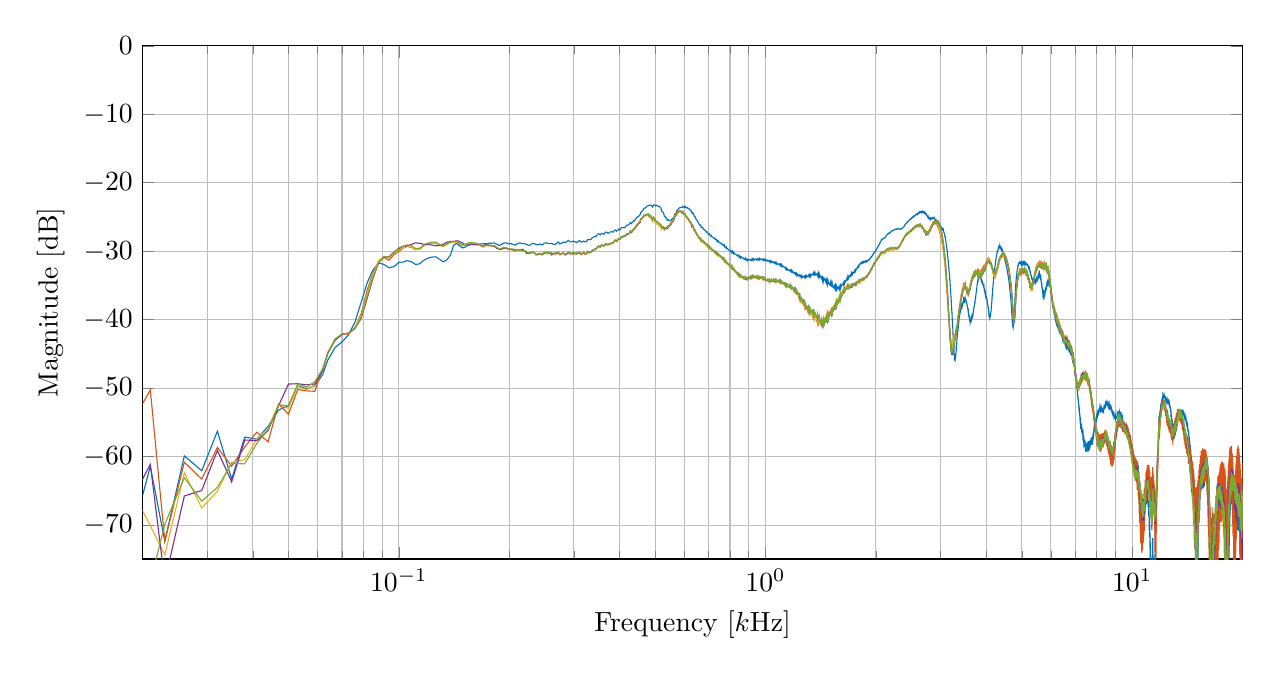
\begin{tikzpicture}

\begin{axis}[%
width=5.5in,
height=2.566in,
at={(1.281in,0.441in)},
scale only axis,
unbounded coords=jump,
xmode=log,
xmin=0.020,
xmax=20.000,
xminorticks=true,
xlabel={Frequency [$k$Hz]},
xmajorgrids,
xminorgrids,
ymin=-74.941,
ymax=0,
ylabel={Magnitude [dB]},
ymajorgrids,
axis background/.style={fill=white},
legend style={legend cell align=left,align=left,draw=white!15!black}
]
\addplot [color=mycolor1,solid,forget plot]
  table[row sep=crcr]{%
0.018	-74.928\\
0.021	-61.394\\
0.023	-72.363\\
0.026	-59.881\\
0.029	-62.051\\
0.032	-56.281\\
0.035	-63.272\\
0.038	-57.140\\
0.041	-57.443\\
0.044	-55.554\\
0.047	-53.186\\
0.050	-52.557\\
0.053	-49.647\\
0.056	-50.077\\
0.059	-49.654\\
0.062	-47.999\\
0.064	-45.903\\
0.067	-44.060\\
0.070	-43.247\\
0.073	-42.156\\
0.076	-40.266\\
0.079	-37.397\\
0.082	-34.567\\
0.085	-32.736\\
0.088	-31.730\\
0.091	-31.908\\
0.094	-32.406\\
0.097	-32.245\\
0.100	-31.616\\
0.103	-31.570\\
0.105	-31.373\\
0.108	-31.505\\
0.111	-31.926\\
0.114	-31.844\\
0.117	-31.312\\
0.120	-31.004\\
0.123	-30.854\\
0.126	-30.808\\
0.129	-31.155\\
0.132	-31.538\\
0.135	-31.280\\
0.138	-30.639\\
0.141	-29.140\\
0.144	-28.816\\
0.146	-29.146\\
0.149	-29.511\\
0.152	-29.378\\
0.155	-29.062\\
0.158	-28.895\\
0.161	-28.940\\
0.164	-28.926\\
0.167	-29.114\\
0.170	-29.221\\
0.173	-28.961\\
0.176	-28.818\\
0.179	-28.832\\
0.182	-28.773\\
0.185	-28.967\\
0.188	-29.156\\
0.190	-29.053\\
0.193	-28.805\\
0.196	-28.768\\
0.199	-28.926\\
0.202	-28.894\\
0.205	-28.990\\
0.208	-29.097\\
0.211	-28.850\\
0.214	-28.776\\
0.217	-28.886\\
0.220	-28.879\\
0.223	-29.016\\
0.226	-29.136\\
0.229	-29.074\\
0.231	-28.855\\
0.234	-28.870\\
0.237	-29.068\\
0.240	-29.011\\
0.243	-28.948\\
0.246	-29.072\\
0.249	-28.831\\
0.252	-28.777\\
0.255	-28.852\\
0.258	-28.857\\
0.261	-28.856\\
0.264	-28.971\\
0.267	-29.022\\
0.270	-28.765\\
0.272	-28.662\\
0.275	-28.938\\
0.278	-28.815\\
0.281	-28.662\\
0.284	-28.758\\
0.287	-28.600\\
0.290	-28.414\\
0.293	-28.626\\
0.296	-28.621\\
0.299	-28.515\\
0.302	-28.616\\
0.305	-28.733\\
0.308	-28.577\\
0.311	-28.433\\
0.313	-28.623\\
0.316	-28.668\\
0.319	-28.499\\
0.322	-28.634\\
0.325	-28.561\\
0.328	-28.254\\
0.331	-28.321\\
0.334	-28.286\\
0.337	-28.012\\
0.340	-27.897\\
0.343	-27.880\\
0.346	-27.745\\
0.349	-27.466\\
0.352	-27.467\\
0.354	-27.621\\
0.357	-27.384\\
0.360	-27.458\\
0.363	-27.512\\
0.366	-27.210\\
0.369	-27.222\\
0.372	-27.383\\
0.375	-27.254\\
0.378	-27.181\\
0.381	-27.132\\
0.384	-27.213\\
0.387	-26.959\\
0.390	-26.886\\
0.393	-27.058\\
0.396	-26.868\\
0.398	-26.761\\
0.401	-26.891\\
0.404	-26.585\\
0.407	-26.533\\
0.410	-26.566\\
0.413	-26.542\\
0.416	-26.372\\
0.419	-26.174\\
0.422	-26.178\\
0.425	-26.050\\
0.428	-25.791\\
0.431	-25.953\\
0.434	-25.731\\
0.437	-25.522\\
0.439	-25.569\\
0.442	-25.312\\
0.445	-25.081\\
0.448	-24.972\\
0.451	-24.877\\
0.454	-24.767\\
0.457	-24.323\\
0.460	-24.195\\
0.463	-24.053\\
0.466	-23.704\\
0.469	-23.708\\
0.472	-23.619\\
0.475	-23.375\\
0.478	-23.367\\
0.480	-23.272\\
0.483	-23.309\\
0.486	-23.264\\
0.489	-23.357\\
0.492	-23.536\\
0.495	-23.232\\
0.498	-23.234\\
0.501	-23.385\\
0.504	-23.269\\
0.507	-23.391\\
0.510	-23.432\\
0.513	-23.425\\
0.516	-23.583\\
0.519	-23.755\\
0.521	-24.160\\
0.524	-24.237\\
0.527	-24.367\\
0.530	-24.927\\
0.533	-24.968\\
0.536	-25.105\\
0.539	-25.470\\
0.542	-25.357\\
0.545	-25.501\\
0.548	-25.545\\
0.551	-25.480\\
0.554	-25.414\\
0.557	-25.198\\
0.560	-25.200\\
0.563	-24.992\\
0.565	-24.556\\
0.568	-24.594\\
0.571	-24.317\\
0.574	-24.019\\
0.577	-23.955\\
0.580	-23.736\\
0.583	-23.653\\
0.586	-23.622\\
0.589	-23.586\\
0.592	-23.623\\
0.595	-23.416\\
0.598	-23.519\\
0.601	-23.634\\
0.604	-23.457\\
0.606	-23.584\\
0.609	-23.679\\
0.612	-23.599\\
0.615	-23.755\\
0.618	-23.760\\
0.621	-23.932\\
0.624	-23.976\\
0.627	-24.119\\
0.630	-24.424\\
0.633	-24.360\\
0.636	-24.488\\
0.639	-24.907\\
0.642	-24.895\\
0.645	-25.168\\
0.647	-25.361\\
0.650	-25.453\\
0.653	-25.691\\
0.656	-25.790\\
0.659	-26.058\\
0.662	-26.175\\
0.665	-26.152\\
0.668	-26.553\\
0.671	-26.482\\
0.674	-26.502\\
0.677	-26.788\\
0.680	-26.799\\
0.683	-26.925\\
0.686	-27.047\\
0.688	-27.036\\
0.691	-27.233\\
0.694	-27.190\\
0.697	-27.407\\
0.700	-27.532\\
0.703	-27.438\\
0.706	-27.671\\
0.709	-27.788\\
0.712	-27.692\\
0.715	-27.917\\
0.718	-27.939\\
0.721	-28.032\\
0.724	-28.109\\
0.727	-28.079\\
0.729	-28.276\\
0.732	-28.238\\
0.735	-28.256\\
0.738	-28.618\\
0.741	-28.455\\
0.744	-28.508\\
0.747	-28.744\\
0.750	-28.727\\
0.753	-28.776\\
0.756	-28.869\\
0.759	-28.937\\
0.762	-29.041\\
0.765	-28.961\\
0.768	-29.195\\
0.771	-29.226\\
0.773	-29.116\\
0.776	-29.504\\
0.779	-29.500\\
0.782	-29.381\\
0.785	-29.655\\
0.788	-29.629\\
0.791	-29.711\\
0.794	-29.824\\
0.797	-29.860\\
0.800	-29.980\\
0.803	-29.867\\
0.806	-30.013\\
0.809	-30.199\\
0.812	-29.988\\
0.814	-30.212\\
0.817	-30.371\\
0.820	-30.180\\
0.823	-30.374\\
0.826	-30.404\\
0.829	-30.437\\
0.832	-30.554\\
0.835	-30.543\\
0.838	-30.681\\
0.841	-30.587\\
0.844	-30.552\\
0.847	-30.870\\
0.850	-30.698\\
0.853	-30.717\\
0.855	-30.955\\
0.858	-30.798\\
0.861	-30.854\\
0.864	-30.969\\
0.867	-30.955\\
0.870	-31.087\\
0.873	-31.026\\
0.876	-31.176\\
0.879	-31.197\\
0.882	-31.031\\
0.885	-31.300\\
0.888	-31.333\\
0.891	-31.144\\
0.894	-31.366\\
0.896	-31.263\\
0.899	-31.204\\
0.902	-31.281\\
0.905	-31.238\\
0.908	-31.294\\
0.911	-31.191\\
0.914	-31.193\\
0.917	-31.336\\
0.920	-31.057\\
0.923	-31.161\\
0.926	-31.337\\
0.929	-31.136\\
0.932	-31.217\\
0.935	-31.236\\
0.938	-31.131\\
0.940	-31.210\\
0.943	-31.167\\
0.946	-31.272\\
0.949	-31.201\\
0.952	-31.085\\
0.955	-31.276\\
0.958	-31.141\\
0.961	-31.032\\
0.964	-31.271\\
0.967	-31.142\\
0.970	-31.131\\
0.973	-31.201\\
0.976	-31.133\\
0.979	-31.191\\
0.981	-31.152\\
0.984	-31.275\\
0.987	-31.352\\
0.990	-31.145\\
0.993	-31.327\\
0.996	-31.374\\
0.999	-31.201\\
1.002	-31.402\\
1.005	-31.423\\
1.008	-31.309\\
1.011	-31.386\\
1.014	-31.315\\
1.017	-31.412\\
1.020	-31.372\\
1.022	-31.393\\
1.025	-31.556\\
1.028	-31.357\\
1.031	-31.376\\
1.034	-31.604\\
1.037	-31.445\\
1.040	-31.540\\
1.043	-31.644\\
1.046	-31.560\\
1.049	-31.626\\
1.052	-31.584\\
1.055	-31.701\\
1.058	-31.735\\
1.061	-31.607\\
1.063	-31.837\\
1.066	-31.771\\
1.069	-31.626\\
1.072	-31.863\\
1.075	-31.801\\
1.078	-31.785\\
1.081	-31.910\\
1.084	-31.856\\
1.087	-31.902\\
1.090	-31.846\\
1.093	-31.929\\
1.096	-32.078\\
1.099	-31.901\\
1.102	-32.040\\
1.104	-32.179\\
1.107	-31.965\\
1.110	-32.135\\
1.113	-32.233\\
1.116	-32.171\\
1.119	-32.266\\
1.122	-32.259\\
1.125	-32.354\\
1.128	-32.328\\
1.131	-32.303\\
1.134	-32.577\\
1.137	-32.473\\
1.140	-32.437\\
1.143	-32.692\\
1.146	-32.557\\
1.148	-32.561\\
1.151	-32.752\\
1.154	-32.731\\
1.157	-32.779\\
1.160	-32.749\\
1.163	-32.829\\
1.166	-32.876\\
1.169	-32.752\\
1.172	-32.999\\
1.175	-33.053\\
1.178	-32.839\\
1.181	-33.058\\
1.184	-33.063\\
1.187	-32.937\\
1.189	-33.117\\
1.192	-33.154\\
1.195	-33.174\\
1.198	-33.112\\
1.201	-33.130\\
1.204	-33.299\\
1.207	-33.144\\
1.210	-33.255\\
1.213	-33.489\\
1.216	-33.230\\
1.219	-33.326\\
1.222	-33.497\\
1.225	-33.375\\
1.228	-33.486\\
1.230	-33.553\\
1.233	-33.590\\
1.236	-33.593\\
1.239	-33.489\\
1.242	-33.714\\
1.245	-33.676\\
1.248	-33.575\\
1.251	-33.845\\
1.254	-33.693\\
1.257	-33.566\\
1.260	-33.787\\
1.263	-33.705\\
1.266	-33.725\\
1.269	-33.757\\
1.271	-33.729\\
1.274	-33.805\\
1.277	-33.644\\
1.280	-33.732\\
1.283	-33.872\\
1.286	-33.612\\
1.289	-33.771\\
1.292	-33.801\\
1.295	-33.562\\
1.298	-33.666\\
1.301	-33.666\\
1.304	-33.638\\
1.307	-33.614\\
1.310	-33.508\\
1.313	-33.629\\
1.315	-33.470\\
1.318	-33.392\\
1.321	-33.676\\
1.324	-33.444\\
1.327	-33.383\\
1.330	-33.608\\
1.333	-33.385\\
1.336	-33.371\\
1.339	-33.450\\
1.342	-33.444\\
1.345	-33.451\\
1.348	-33.270\\
1.351	-33.432\\
1.354	-33.422\\
1.356	-33.163\\
1.359	-33.500\\
1.362	-33.461\\
1.365	-33.200\\
1.368	-33.449\\
1.371	-33.408\\
1.374	-33.319\\
1.377	-33.402\\
1.380	-33.434\\
1.383	-33.532\\
1.386	-33.309\\
1.389	-33.420\\
1.392	-33.627\\
1.395	-33.273\\
1.397	-33.489\\
1.400	-33.730\\
1.403	-33.366\\
1.406	-33.543\\
1.409	-33.680\\
1.412	-33.588\\
1.415	-33.628\\
1.418	-33.686\\
1.421	-33.890\\
1.424	-33.696\\
1.427	-33.681\\
1.430	-34.110\\
1.433	-33.755\\
1.436	-33.793\\
1.438	-34.254\\
1.441	-33.923\\
1.444	-33.904\\
1.447	-34.180\\
1.450	-34.103\\
1.453	-34.088\\
1.456	-34.110\\
1.459	-34.375\\
1.462	-34.219\\
1.465	-34.076\\
1.468	-34.571\\
1.471	-34.375\\
1.474	-34.200\\
1.477	-34.727\\
1.479	-34.535\\
1.482	-34.395\\
1.485	-34.723\\
1.488	-34.684\\
1.491	-34.658\\
1.494	-34.687\\
1.497	-34.880\\
1.500	-34.849\\
1.503	-34.604\\
1.506	-35.004\\
1.509	-34.986\\
1.512	-34.678\\
1.515	-35.117\\
1.518	-35.101\\
1.521	-34.818\\
1.523	-35.146\\
1.526	-35.211\\
1.529	-35.124\\
1.532	-35.189\\
1.535	-35.329\\
1.538	-35.370\\
1.541	-35.129\\
1.544	-35.346\\
1.547	-35.505\\
1.550	-35.108\\
1.553	-35.392\\
1.556	-35.530\\
1.559	-35.114\\
1.562	-35.370\\
1.564	-35.522\\
1.567	-35.264\\
1.570	-35.380\\
1.573	-35.438\\
1.576	-35.399\\
1.579	-35.293\\
1.582	-35.350\\
1.585	-35.503\\
1.588	-35.209\\
1.591	-35.270\\
1.594	-35.474\\
1.597	-35.056\\
1.600	-35.150\\
1.603	-35.334\\
1.605	-34.992\\
1.608	-35.102\\
1.611	-35.123\\
1.614	-34.936\\
1.617	-34.910\\
1.620	-34.842\\
1.623	-34.876\\
1.626	-34.713\\
1.629	-34.646\\
1.632	-34.808\\
1.635	-34.529\\
1.638	-34.476\\
1.641	-34.684\\
1.644	-34.379\\
1.646	-34.403\\
1.649	-34.501\\
1.652	-34.285\\
1.655	-34.262\\
1.658	-34.235\\
1.661	-34.182\\
1.664	-34.145\\
1.667	-33.987\\
1.670	-34.110\\
1.673	-33.958\\
1.676	-33.752\\
1.679	-33.954\\
1.682	-33.782\\
1.685	-33.674\\
1.688	-33.827\\
1.690	-33.668\\
1.693	-33.639\\
1.696	-33.668\\
1.699	-33.578\\
1.702	-33.654\\
1.705	-33.508\\
1.708	-33.599\\
1.711	-33.581\\
1.714	-33.308\\
1.717	-33.495\\
1.720	-33.428\\
1.723	-33.235\\
1.726	-33.378\\
1.729	-33.255\\
1.731	-33.143\\
1.734	-33.173\\
1.737	-33.090\\
1.740	-33.137\\
1.743	-33.014\\
1.746	-32.998\\
1.749	-33.042\\
1.752	-32.821\\
1.755	-32.887\\
1.758	-32.942\\
1.761	-32.722\\
1.764	-32.794\\
1.767	-32.709\\
1.770	-32.547\\
1.772	-32.567\\
1.775	-32.486\\
1.778	-32.465\\
1.781	-32.394\\
1.784	-32.286\\
1.787	-32.332\\
1.790	-32.153\\
1.793	-32.114\\
1.796	-32.207\\
1.799	-31.986\\
1.802	-32.015\\
1.805	-32.006\\
1.808	-31.856\\
1.811	-31.883\\
1.813	-31.827\\
1.816	-31.809\\
1.819	-31.807\\
1.822	-31.685\\
1.825	-31.732\\
1.828	-31.664\\
1.831	-31.606\\
1.834	-31.724\\
1.837	-31.618\\
1.840	-31.599\\
1.843	-31.660\\
1.846	-31.531\\
1.849	-31.588\\
1.852	-31.612\\
1.854	-31.547\\
1.857	-31.612\\
1.860	-31.519\\
1.863	-31.532\\
1.866	-31.531\\
1.869	-31.446\\
1.872	-31.551\\
1.875	-31.516\\
1.878	-31.441\\
1.881	-31.519\\
1.884	-31.412\\
1.887	-31.428\\
1.890	-31.478\\
1.893	-31.407\\
1.896	-31.446\\
1.898	-31.373\\
1.901	-31.326\\
1.904	-31.364\\
1.907	-31.277\\
1.910	-31.308\\
1.913	-31.303\\
1.916	-31.191\\
1.919	-31.207\\
1.922	-31.109\\
1.925	-31.071\\
1.928	-31.102\\
1.931	-31.012\\
1.934	-31.008\\
1.937	-30.956\\
1.939	-30.847\\
1.942	-30.873\\
1.945	-30.811\\
1.948	-30.772\\
1.951	-30.768\\
1.954	-30.634\\
1.957	-30.614\\
1.960	-30.546\\
1.963	-30.461\\
1.966	-30.484\\
1.969	-30.390\\
1.972	-30.330\\
1.975	-30.297\\
1.978	-30.180\\
1.980	-30.180\\
1.983	-30.170\\
1.986	-30.115\\
1.989	-30.123\\
1.992	-30.018\\
1.995	-29.942\\
1.998	-29.906\\
2.001	-29.842\\
2.004	-29.817\\
2.007	-29.752\\
2.010	-29.646\\
2.013	-29.615\\
2.016	-29.503\\
2.019	-29.446\\
2.021	-29.441\\
2.024	-29.353\\
2.027	-29.323\\
2.030	-29.237\\
2.033	-29.142\\
2.036	-29.131\\
2.039	-29.059\\
2.042	-29.025\\
2.045	-28.989\\
2.048	-28.872\\
2.051	-28.821\\
2.054	-28.730\\
2.057	-28.644\\
2.060	-28.625\\
2.063	-28.552\\
2.065	-28.487\\
2.068	-28.425\\
2.071	-28.319\\
2.074	-28.310\\
2.077	-28.278\\
2.080	-28.262\\
2.083	-28.283\\
2.086	-28.207\\
2.089	-28.188\\
2.092	-28.186\\
2.095	-28.150\\
2.098	-28.181\\
2.101	-28.173\\
2.104	-28.129\\
2.106	-28.116\\
2.109	-28.051\\
2.112	-28.035\\
2.115	-28.023\\
2.118	-27.981\\
2.121	-27.993\\
2.124	-27.910\\
2.127	-27.835\\
2.130	-27.811\\
2.133	-27.746\\
2.136	-27.744\\
2.139	-27.713\\
2.142	-27.643\\
2.145	-27.609\\
2.147	-27.537\\
2.150	-27.528\\
2.153	-27.516\\
2.156	-27.471\\
2.159	-27.486\\
2.162	-27.438\\
2.165	-27.371\\
2.168	-27.389\\
2.171	-27.367\\
2.174	-27.376\\
2.177	-27.384\\
2.180	-27.352\\
2.183	-27.320\\
2.186	-27.265\\
2.188	-27.255\\
2.191	-27.258\\
2.194	-27.185\\
2.197	-27.160\\
2.200	-27.118\\
2.203	-27.033\\
2.206	-27.038\\
2.209	-27.030\\
2.212	-27.031\\
2.215	-27.039\\
2.218	-27.018\\
2.221	-26.998\\
2.224	-26.969\\
2.227	-26.952\\
2.229	-26.990\\
2.232	-26.971\\
2.235	-26.938\\
2.238	-26.921\\
2.241	-26.865\\
2.244	-26.848\\
2.247	-26.863\\
2.250	-26.860\\
2.253	-26.859\\
2.256	-26.836\\
2.259	-26.820\\
2.262	-26.794\\
2.265	-26.767\\
2.268	-26.793\\
2.271	-26.794\\
2.273	-26.766\\
2.276	-26.763\\
2.279	-26.747\\
2.282	-26.734\\
2.285	-26.759\\
2.288	-26.794\\
2.291	-26.783\\
2.294	-26.744\\
2.297	-26.734\\
2.300	-26.720\\
2.303	-26.716\\
2.306	-26.730\\
2.309	-26.749\\
2.312	-26.734\\
2.314	-26.724\\
2.317	-26.738\\
2.320	-26.737\\
2.323	-26.758\\
2.326	-26.802\\
2.329	-26.808\\
2.332	-26.775\\
2.335	-26.743\\
2.338	-26.753\\
2.341	-26.758\\
2.344	-26.746\\
2.347	-26.758\\
2.350	-26.727\\
2.353	-26.672\\
2.355	-26.661\\
2.358	-26.645\\
2.361	-26.620\\
2.364	-26.619\\
2.367	-26.613\\
2.370	-26.550\\
2.373	-26.492\\
2.376	-26.475\\
2.379	-26.452\\
2.382	-26.427\\
2.385	-26.402\\
2.388	-26.358\\
2.391	-26.275\\
2.394	-26.218\\
2.396	-26.222\\
2.399	-26.165\\
2.402	-26.118\\
2.405	-26.107\\
2.408	-26.034\\
2.411	-25.994\\
2.414	-25.949\\
2.417	-25.942\\
2.420	-25.945\\
2.423	-25.905\\
2.426	-25.901\\
2.429	-25.839\\
2.432	-25.782\\
2.435	-25.815\\
2.438	-25.800\\
2.440	-25.772\\
2.443	-25.743\\
2.446	-25.686\\
2.449	-25.661\\
2.452	-25.607\\
2.455	-25.591\\
2.458	-25.592\\
2.461	-25.518\\
2.464	-25.504\\
2.467	-25.468\\
2.470	-25.381\\
2.473	-25.395\\
2.476	-25.399\\
2.479	-25.387\\
2.481	-25.361\\
2.484	-25.296\\
2.487	-25.300\\
2.490	-25.271\\
2.493	-25.251\\
2.496	-25.283\\
2.499	-25.205\\
2.502	-25.174\\
2.505	-25.170\\
2.508	-25.087\\
2.511	-25.085\\
2.514	-25.086\\
2.517	-25.072\\
2.520	-25.054\\
2.522	-24.972\\
2.525	-24.977\\
2.528	-24.970\\
2.531	-24.927\\
2.534	-24.975\\
2.537	-24.930\\
2.540	-24.867\\
2.543	-24.884\\
2.546	-24.828\\
2.549	-24.824\\
2.552	-24.821\\
2.555	-24.797\\
2.558	-24.804\\
2.561	-24.709\\
2.563	-24.692\\
2.566	-24.717\\
2.569	-24.656\\
2.572	-24.696\\
2.575	-24.674\\
2.578	-24.594\\
2.581	-24.609\\
2.584	-24.572\\
2.587	-24.589\\
2.590	-24.584\\
2.593	-24.550\\
2.596	-24.602\\
2.599	-24.531\\
2.602	-24.491\\
2.604	-24.544\\
2.607	-24.487\\
2.610	-24.504\\
2.613	-24.503\\
2.616	-24.415\\
2.619	-24.413\\
2.622	-24.373\\
2.625	-24.394\\
2.628	-24.384\\
2.631	-24.302\\
2.634	-24.352\\
2.637	-24.302\\
2.640	-24.219\\
2.643	-24.284\\
2.646	-24.255\\
2.648	-24.261\\
2.651	-24.291\\
2.654	-24.241\\
2.657	-24.247\\
2.660	-24.231\\
2.663	-24.271\\
2.666	-24.335\\
2.669	-24.238\\
2.672	-24.282\\
2.675	-24.294\\
2.678	-24.215\\
2.681	-24.266\\
2.684	-24.247\\
2.687	-24.243\\
2.689	-24.272\\
2.692	-24.220\\
2.695	-24.258\\
2.698	-24.231\\
2.701	-24.255\\
2.704	-24.371\\
2.707	-24.305\\
2.710	-24.317\\
2.713	-24.384\\
2.716	-24.330\\
2.719	-24.403\\
2.722	-24.421\\
2.725	-24.427\\
2.728	-24.483\\
2.730	-24.449\\
2.733	-24.513\\
2.736	-24.512\\
2.739	-24.494\\
2.742	-24.659\\
2.745	-24.649\\
2.748	-24.627\\
2.751	-24.718\\
2.754	-24.706\\
2.757	-24.797\\
2.760	-24.851\\
2.763	-24.870\\
2.766	-24.955\\
2.769	-24.921\\
2.771	-25.006\\
2.774	-25.060\\
2.777	-24.988\\
2.780	-25.129\\
2.783	-25.151\\
2.786	-25.104\\
2.789	-25.159\\
2.792	-25.137\\
2.795	-25.192\\
2.798	-25.228\\
2.801	-25.207\\
2.804	-25.269\\
2.807	-25.198\\
2.810	-25.236\\
2.813	-25.289\\
2.815	-25.174\\
2.818	-25.223\\
2.821	-25.279\\
2.824	-25.221\\
2.827	-25.224\\
2.830	-25.177\\
2.833	-25.197\\
2.836	-25.219\\
2.839	-25.194\\
2.842	-25.222\\
2.845	-25.150\\
2.848	-25.120\\
2.851	-25.194\\
2.854	-25.125\\
2.856	-25.111\\
2.859	-25.177\\
2.862	-25.165\\
2.865	-25.157\\
2.868	-25.114\\
2.871	-25.119\\
2.874	-25.178\\
2.877	-25.180\\
2.880	-25.220\\
2.883	-25.197\\
2.886	-25.139\\
2.889	-25.232\\
2.892	-25.254\\
2.895	-25.243\\
2.897	-25.310\\
2.900	-25.328\\
2.903	-25.377\\
2.906	-25.362\\
2.909	-25.383\\
2.912	-25.494\\
2.915	-25.546\\
2.918	-25.594\\
2.921	-25.633\\
2.924	-25.572\\
2.927	-25.657\\
2.930	-25.782\\
2.933	-25.802\\
2.936	-25.837\\
2.938	-25.857\\
2.941	-25.900\\
2.944	-25.929\\
2.947	-25.893\\
2.950	-26.022\\
2.953	-26.097\\
2.956	-26.100\\
2.959	-26.141\\
2.962	-26.091\\
2.965	-26.113\\
2.968	-26.274\\
2.971	-26.315\\
2.974	-26.300\\
2.977	-26.269\\
2.979	-26.298\\
2.982	-26.362\\
2.985	-26.291\\
2.988	-26.374\\
2.991	-26.464\\
2.994	-26.393\\
2.997	-26.441\\
3.000	-26.388\\
3.003	-26.351\\
3.006	-26.507\\
3.009	-26.566\\
3.012	-26.551\\
3.015	-26.482\\
3.018	-26.480\\
3.021	-26.607\\
3.023	-26.592\\
3.026	-26.625\\
3.029	-26.742\\
3.032	-26.702\\
3.035	-26.725\\
3.038	-26.744\\
3.041	-26.717\\
3.044	-26.848\\
3.047	-26.940\\
3.050	-26.969\\
3.053	-26.916\\
3.056	-26.880\\
3.059	-27.084\\
3.062	-27.147\\
3.064	-27.160\\
3.067	-27.291\\
3.070	-27.307\\
3.073	-27.380\\
3.076	-27.481\\
3.079	-27.505\\
3.082	-27.671\\
3.085	-27.822\\
3.088	-27.935\\
3.091	-28.004\\
3.094	-27.981\\
3.097	-28.212\\
3.100	-28.432\\
3.103	-28.514\\
3.105	-28.700\\
3.108	-28.767\\
3.111	-28.896\\
3.114	-29.098\\
3.117	-29.213\\
3.120	-29.463\\
3.123	-29.632\\
3.126	-29.798\\
3.129	-30.019\\
3.132	-30.011\\
3.135	-30.242\\
3.138	-30.616\\
3.141	-30.804\\
3.144	-31.007\\
3.146	-31.127\\
3.149	-31.319\\
3.152	-31.614\\
3.155	-31.787\\
3.158	-32.122\\
3.161	-32.358\\
3.164	-32.488\\
3.167	-32.854\\
3.170	-32.978\\
3.173	-33.139\\
3.176	-33.610\\
3.179	-33.886\\
3.182	-34.209\\
3.185	-34.339\\
3.188	-34.556\\
3.190	-35.028\\
3.193	-35.264\\
3.196	-35.696\\
3.199	-36.145\\
3.202	-36.185\\
3.205	-36.665\\
3.208	-37.037\\
3.211	-37.245\\
3.214	-37.761\\
3.217	-38.161\\
3.220	-38.559\\
3.223	-38.850\\
3.226	-38.970\\
3.229	-39.625\\
3.231	-40.010\\
3.234	-40.317\\
3.237	-41.063\\
3.240	-41.054\\
3.243	-41.346\\
3.246	-42.142\\
3.249	-42.315\\
3.252	-42.869\\
3.255	-43.332\\
3.258	-43.651\\
3.261	-44.072\\
3.264	-44.045\\
3.267	-44.669\\
3.270	-45.188\\
3.272	-45.013\\
3.275	-45.637\\
3.278	-45.595\\
3.281	-45.156\\
3.284	-45.939\\
3.287	-45.967\\
3.290	-45.474\\
3.293	-45.795\\
3.296	-45.458\\
3.299	-45.193\\
3.302	-45.222\\
3.305	-44.882\\
3.308	-44.870\\
3.311	-44.575\\
3.313	-44.133\\
3.316	-44.154\\
3.319	-43.442\\
3.322	-43.372\\
3.325	-43.531\\
3.328	-42.821\\
3.331	-42.697\\
3.334	-42.511\\
3.337	-42.129\\
3.340	-42.073\\
3.343	-41.808\\
3.346	-41.661\\
3.349	-41.574\\
3.352	-41.174\\
3.354	-41.171\\
3.357	-40.793\\
3.360	-40.494\\
3.363	-40.640\\
3.366	-40.303\\
3.369	-40.019\\
3.372	-40.033\\
3.375	-39.699\\
3.378	-39.665\\
3.381	-39.542\\
3.384	-39.371\\
3.387	-39.361\\
3.390	-39.080\\
3.393	-39.014\\
3.396	-38.983\\
3.398	-38.648\\
3.401	-38.798\\
3.404	-38.758\\
3.407	-38.484\\
3.410	-38.433\\
3.413	-38.301\\
3.416	-38.241\\
3.419	-38.215\\
3.422	-38.043\\
3.425	-38.112\\
3.428	-37.908\\
3.431	-37.818\\
3.434	-37.927\\
3.437	-37.715\\
3.439	-37.741\\
3.442	-37.823\\
3.445	-37.635\\
3.448	-37.623\\
3.451	-37.523\\
3.454	-37.488\\
3.457	-37.540\\
3.460	-37.398\\
3.463	-37.415\\
3.466	-37.301\\
3.469	-37.108\\
3.472	-37.228\\
3.475	-37.171\\
3.478	-37.075\\
3.480	-37.160\\
3.483	-37.066\\
3.486	-37.040\\
3.489	-36.979\\
3.492	-36.928\\
3.495	-37.081\\
3.498	-36.977\\
3.501	-37.041\\
3.504	-37.089\\
3.507	-36.920\\
3.510	-37.031\\
3.513	-37.133\\
3.516	-37.119\\
3.519	-37.208\\
3.521	-37.179\\
3.524	-37.251\\
3.527	-37.282\\
3.530	-37.299\\
3.533	-37.527\\
3.536	-37.586\\
3.539	-37.589\\
3.542	-37.788\\
3.545	-37.777\\
3.548	-37.870\\
3.551	-38.057\\
3.554	-38.165\\
3.557	-38.291\\
3.560	-38.305\\
3.563	-38.387\\
3.565	-38.565\\
3.568	-38.560\\
3.571	-38.804\\
3.574	-38.991\\
3.577	-38.890\\
3.580	-39.120\\
3.583	-39.235\\
3.586	-39.270\\
3.589	-39.477\\
3.592	-39.589\\
3.595	-39.701\\
3.598	-39.736\\
3.601	-39.705\\
3.604	-39.941\\
3.606	-39.922\\
3.609	-40.000\\
3.612	-40.241\\
3.615	-40.119\\
3.618	-40.048\\
3.621	-40.259\\
3.624	-40.154\\
3.627	-40.190\\
3.630	-40.210\\
3.633	-40.232\\
3.636	-40.143\\
3.639	-40.055\\
3.642	-40.063\\
3.645	-40.084\\
3.647	-39.900\\
3.650	-39.985\\
3.653	-39.904\\
3.656	-39.654\\
3.659	-39.763\\
3.662	-39.716\\
3.665	-39.572\\
3.668	-39.556\\
3.671	-39.442\\
3.674	-39.346\\
3.677	-39.189\\
3.680	-39.089\\
3.683	-39.124\\
3.686	-38.916\\
3.688	-38.846\\
3.691	-38.855\\
3.694	-38.516\\
3.697	-38.435\\
3.700	-38.437\\
3.703	-38.232\\
3.706	-38.154\\
3.709	-38.056\\
3.712	-37.959\\
3.715	-37.755\\
3.718	-37.617\\
3.721	-37.626\\
3.724	-37.499\\
3.727	-37.277\\
3.729	-37.301\\
3.732	-37.075\\
3.735	-36.900\\
3.738	-36.891\\
3.741	-36.763\\
3.744	-36.563\\
3.747	-36.458\\
3.750	-36.303\\
3.753	-36.162\\
3.756	-35.928\\
3.759	-35.873\\
3.762	-35.768\\
3.765	-35.469\\
3.768	-35.389\\
3.771	-35.279\\
3.773	-35.018\\
3.776	-34.936\\
3.779	-34.858\\
3.782	-34.720\\
3.785	-34.574\\
3.788	-34.446\\
3.791	-34.394\\
3.794	-34.226\\
3.797	-34.154\\
3.800	-34.210\\
3.803	-34.038\\
3.806	-33.923\\
3.809	-33.936\\
3.812	-33.833\\
3.814	-33.784\\
3.817	-33.786\\
3.820	-33.804\\
3.823	-33.731\\
3.826	-33.645\\
3.829	-33.696\\
3.832	-33.697\\
3.835	-33.591\\
3.838	-33.744\\
3.841	-33.733\\
3.844	-33.647\\
3.847	-33.699\\
3.850	-33.750\\
3.853	-33.756\\
3.855	-33.783\\
3.858	-33.858\\
3.861	-33.929\\
3.864	-33.816\\
3.867	-33.884\\
3.870	-34.001\\
3.873	-33.939\\
3.876	-34.028\\
3.879	-34.165\\
3.882	-34.096\\
3.885	-34.130\\
3.888	-34.197\\
3.891	-34.293\\
3.894	-34.293\\
3.896	-34.379\\
3.899	-34.527\\
3.902	-34.454\\
3.905	-34.444\\
3.908	-34.673\\
3.911	-34.654\\
3.914	-34.680\\
3.917	-34.837\\
3.920	-34.863\\
3.923	-34.826\\
3.926	-34.877\\
3.929	-35.048\\
3.932	-35.077\\
3.935	-35.108\\
3.938	-35.282\\
3.940	-35.321\\
3.943	-35.217\\
3.946	-35.444\\
3.949	-35.588\\
3.952	-35.547\\
3.955	-35.691\\
3.958	-35.786\\
3.961	-35.752\\
3.964	-35.788\\
3.967	-35.969\\
3.970	-36.088\\
3.973	-36.057\\
3.976	-36.165\\
3.979	-36.297\\
3.981	-36.163\\
3.984	-36.272\\
3.987	-36.518\\
3.990	-36.494\\
3.993	-36.547\\
3.996	-36.654\\
3.999	-36.666\\
4.002	-36.660\\
4.005	-36.808\\
4.008	-36.958\\
4.011	-36.978\\
4.014	-36.967\\
4.017	-37.165\\
4.020	-37.162\\
4.022	-37.151\\
4.025	-37.471\\
4.028	-37.539\\
4.031	-37.537\\
4.034	-37.697\\
4.037	-37.772\\
4.040	-37.853\\
4.043	-37.999\\
4.046	-38.253\\
4.049	-38.389\\
4.052	-38.337\\
4.055	-38.557\\
4.058	-38.685\\
4.061	-38.642\\
4.063	-38.973\\
4.066	-39.167\\
4.069	-39.098\\
4.072	-39.210\\
4.075	-39.325\\
4.078	-39.313\\
4.081	-39.455\\
4.084	-39.601\\
4.087	-39.689\\
4.090	-39.471\\
4.093	-39.473\\
4.096	-39.575\\
4.099	-39.452\\
4.102	-39.450\\
4.104	-39.553\\
4.107	-39.242\\
4.110	-39.085\\
4.113	-39.070\\
4.116	-38.895\\
4.119	-38.859\\
4.122	-38.740\\
4.125	-38.546\\
4.128	-38.306\\
4.131	-38.003\\
4.134	-37.936\\
4.137	-37.743\\
4.140	-37.480\\
4.143	-37.382\\
4.146	-37.045\\
4.148	-36.710\\
4.151	-36.612\\
4.154	-36.407\\
4.157	-36.211\\
4.160	-36.046\\
4.163	-35.738\\
4.166	-35.509\\
4.169	-35.226\\
4.172	-35.104\\
4.175	-34.994\\
4.178	-34.739\\
4.181	-34.543\\
4.184	-34.336\\
4.187	-34.068\\
4.189	-33.967\\
4.192	-33.850\\
4.195	-33.731\\
4.198	-33.580\\
4.201	-33.317\\
4.204	-33.169\\
4.207	-33.034\\
4.210	-32.868\\
4.213	-32.846\\
4.216	-32.710\\
4.219	-32.501\\
4.222	-32.359\\
4.225	-32.198\\
4.228	-32.104\\
4.230	-32.002\\
4.233	-31.926\\
4.236	-31.812\\
4.239	-31.559\\
4.242	-31.449\\
4.245	-31.391\\
4.248	-31.220\\
4.251	-31.187\\
4.254	-31.109\\
4.257	-30.912\\
4.260	-30.786\\
4.263	-30.716\\
4.266	-30.648\\
4.269	-30.570\\
4.271	-30.503\\
4.274	-30.461\\
4.277	-30.279\\
4.280	-30.190\\
4.283	-30.215\\
4.286	-30.123\\
4.289	-30.075\\
4.292	-30.078\\
4.295	-29.939\\
4.298	-29.843\\
4.301	-29.811\\
4.304	-29.808\\
4.307	-29.770\\
4.310	-29.703\\
4.313	-29.715\\
4.315	-29.597\\
4.318	-29.491\\
4.321	-29.574\\
4.324	-29.539\\
4.327	-29.480\\
4.330	-29.490\\
4.333	-29.435\\
4.336	-29.352\\
4.339	-29.347\\
4.342	-29.392\\
4.345	-29.408\\
4.348	-29.324\\
4.351	-29.361\\
4.354	-29.357\\
4.356	-29.254\\
4.359	-29.357\\
4.362	-29.413\\
4.365	-29.344\\
4.368	-29.392\\
4.371	-29.411\\
4.374	-29.404\\
4.377	-29.405\\
4.380	-29.468\\
4.383	-29.552\\
4.386	-29.512\\
4.389	-29.554\\
4.392	-29.623\\
4.395	-29.557\\
4.397	-29.616\\
4.400	-29.752\\
4.403	-29.735\\
4.406	-29.754\\
4.409	-29.765\\
4.412	-29.779\\
4.415	-29.795\\
4.418	-29.847\\
4.421	-29.991\\
4.424	-29.962\\
4.427	-29.902\\
4.430	-30.019\\
4.433	-30.030\\
4.436	-30.066\\
4.438	-30.214\\
4.441	-30.238\\
4.444	-30.220\\
4.447	-30.294\\
4.450	-30.371\\
4.453	-30.429\\
4.456	-30.457\\
4.459	-30.573\\
4.462	-30.609\\
4.465	-30.559\\
4.468	-30.687\\
4.471	-30.753\\
4.474	-30.732\\
4.477	-30.855\\
4.479	-30.920\\
4.482	-30.934\\
4.485	-30.974\\
4.488	-31.061\\
4.491	-31.136\\
4.494	-31.136\\
4.497	-31.230\\
4.500	-31.336\\
4.503	-31.284\\
4.506	-31.383\\
4.509	-31.512\\
4.512	-31.507\\
4.515	-31.588\\
4.518	-31.675\\
4.521	-31.731\\
4.523	-31.778\\
4.526	-31.845\\
4.529	-31.975\\
4.532	-32.019\\
4.535	-32.063\\
4.538	-32.216\\
4.541	-32.221\\
4.544	-32.267\\
4.547	-32.424\\
4.550	-32.468\\
4.553	-32.528\\
4.556	-32.636\\
4.559	-32.703\\
4.562	-32.767\\
4.564	-32.835\\
4.567	-32.968\\
4.570	-33.058\\
4.573	-33.068\\
4.576	-33.213\\
4.579	-33.293\\
4.582	-33.307\\
4.585	-33.441\\
4.588	-33.520\\
4.591	-33.602\\
4.594	-33.702\\
4.597	-33.796\\
4.600	-33.899\\
4.603	-33.939\\
4.605	-34.054\\
4.608	-34.221\\
4.611	-34.265\\
4.614	-34.410\\
4.617	-34.604\\
4.620	-34.630\\
4.623	-34.845\\
4.626	-35.000\\
4.629	-35.130\\
4.632	-35.306\\
4.635	-35.409\\
4.638	-35.610\\
4.641	-35.737\\
4.644	-35.824\\
4.646	-36.021\\
4.649	-36.143\\
4.652	-36.197\\
4.655	-36.410\\
4.658	-36.464\\
4.661	-36.613\\
4.664	-36.821\\
4.667	-36.921\\
4.670	-37.158\\
4.673	-37.318\\
4.676	-37.515\\
4.679	-37.790\\
4.682	-37.917\\
4.685	-38.187\\
4.688	-38.454\\
4.690	-38.587\\
4.693	-38.885\\
4.696	-39.105\\
4.699	-39.268\\
4.702	-39.576\\
4.705	-39.692\\
4.708	-39.980\\
4.711	-40.199\\
4.714	-40.354\\
4.717	-40.619\\
4.720	-40.745\\
4.723	-40.741\\
4.726	-41.018\\
4.729	-41.062\\
4.731	-41.125\\
4.734	-41.183\\
4.737	-41.059\\
4.740	-40.998\\
4.743	-40.933\\
4.746	-40.909\\
4.749	-40.847\\
4.752	-40.585\\
4.755	-40.366\\
4.758	-40.224\\
4.761	-39.821\\
4.764	-39.706\\
4.767	-39.559\\
4.770	-39.162\\
4.772	-38.882\\
4.775	-38.595\\
4.778	-38.231\\
4.781	-37.992\\
4.784	-37.721\\
4.787	-37.452\\
4.790	-37.072\\
4.793	-36.714\\
4.796	-36.531\\
4.799	-36.149\\
4.802	-35.890\\
4.805	-35.791\\
4.808	-35.386\\
4.811	-35.117\\
4.813	-34.945\\
4.816	-34.697\\
4.819	-34.507\\
4.822	-34.381\\
4.825	-34.231\\
4.828	-34.034\\
4.831	-33.773\\
4.834	-33.713\\
4.837	-33.576\\
4.840	-33.432\\
4.843	-33.434\\
4.846	-33.229\\
4.849	-33.042\\
4.852	-32.964\\
4.854	-32.865\\
4.857	-32.792\\
4.860	-32.723\\
4.863	-32.640\\
4.866	-32.549\\
4.869	-32.354\\
4.872	-32.314\\
4.875	-32.303\\
4.878	-32.198\\
4.881	-32.219\\
4.884	-32.147\\
4.887	-31.995\\
4.890	-31.961\\
4.893	-31.938\\
4.896	-31.946\\
4.898	-31.924\\
4.901	-31.866\\
4.904	-31.833\\
4.907	-31.728\\
4.910	-31.715\\
4.913	-31.779\\
4.916	-31.752\\
4.919	-31.728\\
4.922	-31.718\\
4.925	-31.653\\
4.928	-31.640\\
4.931	-31.648\\
4.934	-31.733\\
4.937	-31.757\\
4.939	-31.675\\
4.942	-31.704\\
4.945	-31.649\\
4.948	-31.625\\
4.951	-31.748\\
4.954	-31.770\\
4.957	-31.742\\
4.960	-31.706\\
4.963	-31.670\\
4.966	-31.663\\
4.969	-31.701\\
4.972	-31.755\\
4.975	-31.783\\
4.978	-31.709\\
4.980	-31.685\\
4.983	-31.699\\
4.986	-31.662\\
4.989	-31.762\\
4.992	-31.837\\
4.995	-31.764\\
4.998	-31.742\\
5.001	-31.713\\
5.004	-31.719\\
5.007	-31.772\\
5.010	-31.809\\
5.013	-31.850\\
5.016	-31.755\\
5.019	-31.708\\
5.021	-31.756\\
5.024	-31.730\\
5.027	-31.790\\
5.030	-31.857\\
5.033	-31.792\\
5.036	-31.748\\
5.039	-31.713\\
5.042	-31.737\\
5.045	-31.800\\
5.048	-31.820\\
5.051	-31.818\\
5.054	-31.756\\
5.057	-31.669\\
5.060	-31.720\\
5.063	-31.762\\
5.065	-31.775\\
5.068	-31.832\\
5.071	-31.744\\
5.074	-31.710\\
5.077	-31.680\\
5.080	-31.717\\
5.083	-31.803\\
5.086	-31.802\\
5.089	-31.780\\
5.092	-31.780\\
5.095	-31.684\\
5.098	-31.739\\
5.101	-31.827\\
5.104	-31.838\\
5.106	-31.880\\
5.109	-31.830\\
5.112	-31.783\\
5.115	-31.784\\
5.118	-31.833\\
5.121	-31.924\\
5.124	-31.928\\
5.127	-31.858\\
5.130	-31.851\\
5.133	-31.776\\
5.136	-31.822\\
5.139	-31.913\\
5.142	-31.927\\
5.145	-31.918\\
5.147	-31.875\\
5.150	-31.826\\
5.153	-31.836\\
5.156	-31.902\\
5.159	-31.990\\
5.162	-31.986\\
5.165	-31.918\\
5.168	-31.920\\
5.171	-31.916\\
5.174	-31.915\\
5.177	-32.040\\
5.180	-32.059\\
5.183	-32.026\\
5.186	-32.015\\
5.188	-31.993\\
5.191	-32.030\\
5.194	-32.096\\
5.197	-32.166\\
5.200	-32.209\\
5.203	-32.120\\
5.206	-32.119\\
5.209	-32.183\\
5.212	-32.211\\
5.215	-32.339\\
5.218	-32.377\\
5.221	-32.330\\
5.224	-32.317\\
5.227	-32.313\\
5.229	-32.392\\
5.232	-32.463\\
5.235	-32.526\\
5.238	-32.575\\
5.241	-32.518\\
5.244	-32.494\\
5.247	-32.638\\
5.250	-32.667\\
5.253	-32.757\\
5.256	-32.838\\
5.259	-32.802\\
5.262	-32.833\\
5.265	-32.864\\
5.268	-32.976\\
5.271	-33.088\\
5.273	-33.090\\
5.276	-33.160\\
5.279	-33.183\\
5.282	-33.164\\
5.285	-33.267\\
5.288	-33.372\\
5.291	-33.431\\
5.294	-33.460\\
5.297	-33.485\\
5.300	-33.513\\
5.303	-33.540\\
5.306	-33.670\\
5.309	-33.776\\
5.312	-33.750\\
5.314	-33.789\\
5.317	-33.848\\
5.320	-33.814\\
5.323	-33.918\\
5.326	-34.043\\
5.329	-34.053\\
5.332	-34.066\\
5.335	-34.070\\
5.338	-34.119\\
5.341	-34.122\\
5.344	-34.178\\
5.347	-34.306\\
5.350	-34.257\\
5.353	-34.225\\
5.355	-34.345\\
5.358	-34.283\\
5.361	-34.302\\
5.364	-34.426\\
5.367	-34.408\\
5.370	-34.384\\
5.373	-34.373\\
5.376	-34.416\\
5.379	-34.416\\
5.382	-34.380\\
5.385	-34.486\\
5.388	-34.478\\
5.391	-34.393\\
5.394	-34.437\\
5.396	-34.446\\
5.399	-34.396\\
5.402	-34.472\\
5.405	-34.493\\
5.408	-34.431\\
5.411	-34.418\\
5.414	-34.436\\
5.417	-34.474\\
5.420	-34.385\\
5.423	-34.447\\
5.426	-34.493\\
5.429	-34.401\\
5.432	-34.392\\
5.435	-34.439\\
5.438	-34.390\\
5.440	-34.421\\
5.443	-34.432\\
5.446	-34.436\\
5.449	-34.383\\
5.452	-34.315\\
5.455	-34.377\\
5.458	-34.329\\
5.461	-34.283\\
5.464	-34.396\\
5.467	-34.316\\
5.470	-34.235\\
5.473	-34.250\\
5.476	-34.260\\
5.479	-34.234\\
5.481	-34.213\\
5.484	-34.214\\
5.487	-34.203\\
5.490	-34.091\\
5.493	-34.143\\
5.496	-34.188\\
5.499	-34.049\\
5.502	-34.100\\
5.505	-34.101\\
5.508	-34.002\\
5.511	-33.967\\
5.514	-33.998\\
5.517	-34.004\\
5.520	-33.924\\
5.522	-33.923\\
5.525	-33.951\\
5.528	-33.844\\
5.531	-33.769\\
5.534	-33.886\\
5.537	-33.822\\
5.540	-33.776\\
5.543	-33.796\\
5.546	-33.726\\
5.549	-33.651\\
5.552	-33.638\\
5.555	-33.696\\
5.558	-33.663\\
5.561	-33.555\\
5.563	-33.606\\
5.566	-33.550\\
5.569	-33.420\\
5.572	-33.513\\
5.575	-33.543\\
5.578	-33.459\\
5.581	-33.447\\
5.584	-33.441\\
5.587	-33.423\\
5.590	-33.343\\
5.593	-33.465\\
5.596	-33.521\\
5.599	-33.424\\
5.602	-33.427\\
5.604	-33.526\\
5.607	-33.460\\
5.610	-33.469\\
5.613	-33.627\\
5.616	-33.652\\
5.619	-33.640\\
5.622	-33.669\\
5.625	-33.801\\
5.628	-33.759\\
5.631	-33.833\\
5.634	-34.100\\
5.637	-34.123\\
5.640	-34.063\\
5.643	-34.268\\
5.646	-34.351\\
5.648	-34.347\\
5.651	-34.526\\
5.654	-34.676\\
5.657	-34.708\\
5.660	-34.691\\
5.663	-34.846\\
5.666	-34.988\\
5.669	-34.961\\
5.672	-35.203\\
5.675	-35.357\\
5.678	-35.212\\
5.681	-35.321\\
5.684	-35.533\\
5.687	-35.569\\
5.689	-35.623\\
5.692	-35.810\\
5.695	-35.871\\
5.698	-35.765\\
5.701	-35.856\\
5.704	-36.133\\
5.707	-36.067\\
5.710	-36.105\\
5.713	-36.358\\
5.716	-36.226\\
5.719	-36.156\\
5.722	-36.334\\
5.725	-36.439\\
5.728	-36.356\\
5.730	-36.390\\
5.733	-36.487\\
5.736	-36.347\\
5.739	-36.224\\
5.742	-36.506\\
5.745	-36.515\\
5.748	-36.321\\
5.751	-36.413\\
5.754	-36.425\\
5.757	-36.178\\
5.760	-36.225\\
5.763	-36.396\\
5.766	-36.313\\
5.769	-36.098\\
5.771	-36.217\\
5.774	-36.199\\
5.777	-35.917\\
5.780	-36.015\\
5.783	-36.200\\
5.786	-35.965\\
5.789	-35.852\\
5.792	-35.951\\
5.795	-35.851\\
5.798	-35.671\\
5.801	-35.818\\
5.804	-35.903\\
5.807	-35.647\\
5.810	-35.591\\
5.813	-35.722\\
5.815	-35.555\\
5.818	-35.414\\
5.821	-35.600\\
5.824	-35.576\\
5.827	-35.317\\
5.830	-35.324\\
5.833	-35.361\\
5.836	-35.221\\
5.839	-35.143\\
5.842	-35.309\\
5.845	-35.200\\
5.848	-34.881\\
5.851	-34.962\\
5.854	-35.074\\
5.856	-34.820\\
5.859	-34.855\\
5.862	-34.965\\
5.865	-34.782\\
5.868	-34.571\\
5.871	-34.715\\
5.874	-34.751\\
5.877	-34.524\\
5.880	-34.577\\
5.883	-34.722\\
5.886	-34.431\\
5.889	-34.319\\
5.892	-34.578\\
5.895	-34.503\\
5.897	-34.363\\
5.900	-34.480\\
5.903	-34.562\\
5.906	-34.277\\
5.909	-34.259\\
5.912	-34.582\\
5.915	-34.414\\
5.918	-34.273\\
5.921	-34.538\\
5.924	-34.481\\
5.927	-34.231\\
5.930	-34.413\\
5.933	-34.585\\
5.936	-34.428\\
5.938	-34.387\\
5.941	-34.621\\
5.944	-34.551\\
5.947	-34.313\\
5.950	-34.616\\
5.953	-34.777\\
5.956	-34.547\\
5.959	-34.616\\
5.962	-34.839\\
5.965	-34.703\\
5.968	-34.649\\
5.971	-34.952\\
5.974	-35.055\\
5.977	-34.858\\
5.979	-35.022\\
5.982	-35.270\\
5.985	-34.996\\
5.988	-35.099\\
5.991	-35.491\\
5.994	-35.417\\
5.997	-35.279\\
6.000	-35.531\\
6.003	-35.652\\
6.006	-35.513\\
6.009	-35.674\\
6.012	-36.039\\
6.015	-35.930\\
6.018	-35.779\\
6.021	-36.166\\
6.023	-36.221\\
6.026	-36.008\\
6.029	-36.347\\
6.032	-36.633\\
6.035	-36.375\\
6.038	-36.408\\
6.041	-36.700\\
6.044	-36.741\\
6.047	-36.627\\
6.050	-37.008\\
6.053	-37.173\\
6.056	-36.841\\
6.059	-37.008\\
6.062	-37.384\\
6.064	-37.219\\
6.067	-37.237\\
6.070	-37.635\\
6.073	-37.634\\
6.076	-37.388\\
6.079	-37.625\\
6.082	-37.964\\
6.085	-37.761\\
6.088	-37.834\\
6.091	-38.285\\
6.094	-38.103\\
6.097	-37.917\\
6.100	-38.361\\
6.103	-38.480\\
6.105	-38.293\\
6.108	-38.439\\
6.111	-38.760\\
6.114	-38.528\\
6.117	-38.425\\
6.120	-38.940\\
6.123	-38.939\\
6.126	-38.663\\
6.129	-39.078\\
6.132	-39.134\\
6.135	-38.804\\
6.138	-38.968\\
6.141	-39.398\\
6.144	-39.247\\
6.146	-39.096\\
6.149	-39.454\\
6.152	-39.507\\
6.155	-39.097\\
6.158	-39.482\\
6.161	-39.828\\
6.164	-39.481\\
6.167	-39.495\\
6.170	-39.867\\
6.173	-39.625\\
6.176	-39.542\\
6.179	-39.903\\
6.182	-40.109\\
6.185	-39.749\\
6.188	-39.878\\
6.190	-40.233\\
6.193	-39.955\\
6.196	-39.915\\
6.199	-40.496\\
6.202	-40.406\\
6.205	-40.054\\
6.208	-40.381\\
6.211	-40.503\\
6.214	-40.228\\
6.217	-40.414\\
6.220	-40.786\\
6.223	-40.570\\
6.226	-40.262\\
6.229	-40.662\\
6.231	-40.711\\
6.234	-40.374\\
6.237	-40.707\\
6.240	-41.031\\
6.243	-40.551\\
6.246	-40.532\\
6.249	-40.888\\
6.252	-40.760\\
6.255	-40.620\\
6.258	-40.950\\
6.261	-41.090\\
6.264	-40.647\\
6.267	-40.730\\
6.270	-41.158\\
6.272	-40.890\\
6.275	-40.839\\
6.278	-41.274\\
6.281	-41.079\\
6.284	-40.768\\
6.287	-41.075\\
6.290	-41.314\\
6.293	-41.060\\
6.296	-41.108\\
6.299	-41.504\\
6.302	-41.199\\
6.305	-40.966\\
6.308	-41.396\\
6.311	-41.540\\
6.313	-41.227\\
6.316	-41.501\\
6.319	-41.628\\
6.322	-41.297\\
6.325	-41.305\\
6.328	-41.747\\
6.331	-41.728\\
6.334	-41.451\\
6.337	-41.718\\
6.340	-41.819\\
6.343	-41.378\\
6.346	-41.587\\
6.349	-41.968\\
6.352	-41.696\\
6.354	-41.574\\
6.357	-41.898\\
6.360	-41.742\\
6.363	-41.527\\
6.366	-41.838\\
6.369	-42.142\\
6.372	-41.741\\
6.375	-41.698\\
6.378	-42.124\\
6.381	-41.807\\
6.384	-41.677\\
6.387	-42.207\\
6.390	-42.100\\
6.393	-41.797\\
6.396	-41.924\\
6.398	-42.150\\
6.401	-41.917\\
6.404	-41.939\\
6.407	-42.379\\
6.410	-42.232\\
6.413	-41.852\\
6.416	-42.233\\
6.419	-42.274\\
6.422	-41.998\\
6.425	-42.241\\
6.428	-42.474\\
6.431	-42.192\\
6.434	-42.055\\
6.437	-42.358\\
6.439	-42.443\\
6.442	-42.199\\
6.445	-42.470\\
6.448	-42.687\\
6.451	-42.222\\
6.454	-42.262\\
6.457	-42.727\\
6.460	-42.478\\
6.463	-42.449\\
6.466	-42.770\\
6.469	-42.714\\
6.472	-42.450\\
6.475	-42.582\\
6.478	-42.944\\
6.480	-42.736\\
6.483	-42.714\\
6.486	-43.072\\
6.489	-42.852\\
6.492	-42.619\\
6.495	-42.981\\
6.498	-43.095\\
6.501	-42.858\\
6.504	-43.044\\
6.507	-43.175\\
6.510	-42.921\\
6.513	-42.829\\
6.516	-43.176\\
6.519	-43.238\\
6.521	-42.938\\
6.524	-43.199\\
6.527	-43.325\\
6.530	-42.948\\
6.533	-43.128\\
6.536	-43.479\\
6.539	-43.205\\
6.542	-43.140\\
6.545	-43.344\\
6.548	-43.327\\
6.551	-43.092\\
6.554	-43.284\\
6.557	-43.531\\
6.560	-43.227\\
6.563	-43.274\\
6.565	-43.519\\
6.568	-43.306\\
6.571	-43.292\\
6.574	-43.627\\
6.577	-43.581\\
6.580	-43.464\\
6.583	-43.510\\
6.586	-43.689\\
6.589	-43.600\\
6.592	-43.526\\
6.595	-43.865\\
6.598	-43.791\\
6.601	-43.562\\
6.604	-43.712\\
6.606	-43.785\\
6.609	-43.561\\
6.612	-43.786\\
6.615	-43.879\\
6.618	-43.825\\
6.621	-43.681\\
6.624	-43.716\\
6.627	-43.878\\
6.630	-43.691\\
6.633	-43.863\\
6.636	-43.946\\
6.639	-43.692\\
6.642	-43.779\\
6.645	-43.928\\
6.647	-43.888\\
6.650	-43.876\\
6.653	-43.952\\
6.656	-44.046\\
6.659	-43.882\\
6.662	-43.860\\
6.665	-44.058\\
6.668	-44.037\\
6.671	-43.895\\
6.674	-44.101\\
6.677	-43.973\\
6.680	-43.884\\
6.683	-43.945\\
6.686	-44.097\\
6.688	-44.093\\
6.691	-44.046\\
6.694	-44.140\\
6.697	-44.184\\
6.700	-43.940\\
6.703	-44.155\\
6.706	-44.292\\
6.709	-44.165\\
6.712	-44.193\\
6.715	-44.271\\
6.718	-44.197\\
6.721	-44.069\\
6.724	-44.189\\
6.727	-44.379\\
6.729	-44.198\\
6.732	-44.176\\
6.735	-44.282\\
6.738	-44.169\\
6.741	-44.092\\
6.744	-44.412\\
6.747	-44.378\\
6.750	-44.295\\
6.753	-44.406\\
6.756	-44.378\\
6.759	-44.393\\
6.762	-44.432\\
6.765	-44.589\\
6.768	-44.599\\
6.771	-44.378\\
6.773	-44.562\\
6.776	-44.557\\
6.779	-44.459\\
6.782	-44.636\\
6.785	-44.712\\
6.788	-44.649\\
6.791	-44.558\\
6.794	-44.694\\
6.797	-44.747\\
6.800	-44.626\\
6.803	-44.740\\
6.806	-44.955\\
6.809	-44.739\\
6.812	-44.681\\
6.814	-44.918\\
6.817	-44.794\\
6.820	-44.841\\
6.823	-45.055\\
6.826	-44.977\\
6.829	-44.902\\
6.832	-44.794\\
6.835	-45.062\\
6.838	-44.971\\
6.841	-44.959\\
6.844	-45.242\\
6.847	-45.127\\
6.850	-44.953\\
6.853	-45.157\\
6.855	-45.273\\
6.858	-45.211\\
6.861	-45.253\\
6.864	-45.357\\
6.867	-45.368\\
6.870	-45.209\\
6.873	-45.519\\
6.876	-45.635\\
6.879	-45.572\\
6.882	-45.702\\
6.885	-45.774\\
6.888	-45.521\\
6.891	-45.601\\
6.894	-45.832\\
6.896	-45.796\\
6.899	-45.694\\
6.902	-45.827\\
6.905	-45.994\\
6.908	-45.814\\
6.911	-45.875\\
6.914	-46.077\\
6.917	-46.050\\
6.920	-45.992\\
6.923	-46.278\\
6.926	-46.250\\
6.929	-46.117\\
6.932	-46.365\\
6.935	-46.493\\
6.938	-46.402\\
6.940	-46.270\\
6.943	-46.545\\
6.946	-46.575\\
6.949	-46.411\\
6.952	-46.693\\
6.955	-46.799\\
6.958	-46.614\\
6.961	-46.845\\
6.964	-46.997\\
6.967	-46.833\\
6.970	-46.856\\
6.973	-47.156\\
6.976	-47.336\\
6.979	-47.162\\
6.981	-47.300\\
6.984	-47.723\\
6.987	-47.422\\
6.990	-47.511\\
6.993	-48.064\\
6.996	-47.760\\
6.999	-47.773\\
7.002	-48.100\\
7.005	-48.063\\
7.008	-47.959\\
7.011	-48.103\\
7.014	-48.511\\
7.017	-48.402\\
7.020	-48.268\\
7.022	-48.747\\
7.025	-48.625\\
7.028	-48.425\\
7.031	-49.077\\
7.034	-49.001\\
7.037	-48.722\\
7.040	-49.045\\
7.043	-49.265\\
7.046	-49.218\\
7.049	-48.965\\
7.052	-49.554\\
7.055	-49.629\\
7.058	-49.308\\
7.061	-49.641\\
7.063	-49.786\\
7.066	-49.460\\
7.069	-49.765\\
7.072	-50.013\\
7.075	-49.951\\
7.078	-50.099\\
7.081	-50.265\\
7.084	-50.337\\
7.087	-50.318\\
7.090	-50.387\\
7.093	-50.924\\
7.096	-50.766\\
7.099	-50.656\\
7.102	-51.297\\
7.104	-51.145\\
7.107	-50.924\\
7.110	-51.472\\
7.113	-51.629\\
7.116	-51.383\\
7.119	-51.278\\
7.122	-51.791\\
7.125	-51.730\\
7.128	-51.525\\
7.131	-51.921\\
7.134	-52.037\\
7.137	-51.805\\
7.140	-52.166\\
7.143	-52.506\\
7.146	-52.130\\
7.148	-52.548\\
7.151	-52.561\\
7.154	-52.504\\
7.157	-52.314\\
7.160	-52.720\\
7.163	-53.278\\
7.166	-52.777\\
7.169	-52.971\\
7.172	-53.471\\
7.175	-52.919\\
7.178	-52.960\\
7.181	-53.484\\
7.184	-53.737\\
7.187	-53.507\\
7.189	-53.787\\
7.192	-54.053\\
7.195	-53.643\\
7.198	-53.666\\
7.201	-54.671\\
7.204	-54.527\\
7.207	-54.034\\
7.210	-54.668\\
7.213	-54.614\\
7.216	-54.349\\
7.219	-55.046\\
7.222	-55.285\\
7.225	-54.983\\
7.228	-54.639\\
7.230	-55.146\\
7.233	-55.403\\
7.236	-54.655\\
7.239	-55.457\\
7.242	-55.946\\
7.245	-55.154\\
7.248	-55.529\\
7.251	-55.512\\
7.254	-55.345\\
7.257	-55.641\\
7.260	-55.804\\
7.263	-55.685\\
7.266	-55.125\\
7.269	-55.400\\
7.271	-56.038\\
7.274	-55.607\\
7.277	-55.597\\
7.280	-56.383\\
7.283	-55.659\\
7.286	-55.663\\
7.289	-56.495\\
7.292	-56.079\\
7.295	-56.300\\
7.298	-56.375\\
7.301	-56.676\\
7.304	-55.921\\
7.307	-56.084\\
7.310	-56.497\\
7.313	-56.422\\
7.315	-56.164\\
7.318	-56.744\\
7.321	-56.344\\
7.324	-55.969\\
7.327	-56.316\\
7.330	-56.832\\
7.333	-56.741\\
7.336	-57.011\\
7.339	-56.983\\
7.342	-56.989\\
7.345	-56.210\\
7.348	-57.229\\
7.351	-57.705\\
7.354	-57.011\\
7.356	-56.931\\
7.359	-57.640\\
7.362	-57.071\\
7.365	-57.059\\
7.368	-57.597\\
7.371	-57.966\\
7.374	-57.403\\
7.377	-57.382\\
7.380	-57.544\\
7.383	-57.203\\
7.386	-57.236\\
7.389	-58.056\\
7.392	-58.013\\
7.395	-57.461\\
7.397	-57.941\\
7.400	-57.621\\
7.403	-57.666\\
7.406	-58.229\\
7.409	-58.035\\
7.412	-57.686\\
7.415	-57.685\\
7.418	-57.622\\
7.421	-58.524\\
7.424	-57.613\\
7.427	-58.263\\
7.430	-58.528\\
7.433	-57.677\\
7.436	-57.980\\
7.438	-58.014\\
7.441	-57.911\\
7.444	-58.284\\
7.447	-58.527\\
7.450	-58.654\\
7.453	-58.484\\
7.456	-57.980\\
7.459	-59.191\\
7.462	-58.775\\
7.465	-58.273\\
7.468	-59.304\\
7.471	-58.396\\
7.474	-58.373\\
7.477	-58.405\\
7.479	-58.495\\
7.482	-59.018\\
7.485	-58.902\\
7.488	-58.825\\
7.491	-59.194\\
7.494	-58.437\\
7.497	-58.759\\
7.500	-58.778\\
7.503	-58.493\\
7.506	-59.205\\
7.509	-58.569\\
7.512	-58.154\\
7.515	-58.419\\
7.518	-58.600\\
7.521	-58.931\\
7.523	-58.739\\
7.526	-58.425\\
7.529	-58.876\\
7.532	-57.935\\
7.535	-58.307\\
7.538	-59.142\\
7.541	-58.604\\
7.544	-58.577\\
7.547	-59.269\\
7.550	-58.465\\
7.553	-58.535\\
7.556	-58.509\\
7.559	-59.247\\
7.562	-58.707\\
7.564	-58.056\\
7.567	-58.576\\
7.570	-58.268\\
7.573	-57.798\\
7.576	-58.919\\
7.579	-58.695\\
7.582	-58.419\\
7.585	-58.366\\
7.588	-58.135\\
7.591	-58.507\\
7.594	-58.095\\
7.597	-58.940\\
7.600	-59.240\\
7.603	-57.738\\
7.605	-57.902\\
7.608	-58.206\\
7.611	-57.980\\
7.614	-58.489\\
7.617	-58.329\\
7.620	-58.259\\
7.623	-58.166\\
7.626	-57.953\\
7.629	-58.429\\
7.632	-58.383\\
7.635	-58.069\\
7.638	-59.054\\
7.641	-58.288\\
7.644	-57.663\\
7.646	-58.483\\
7.649	-58.204\\
7.652	-58.129\\
7.655	-57.984\\
7.658	-58.095\\
7.661	-58.330\\
7.664	-57.867\\
7.667	-58.112\\
7.670	-58.299\\
7.673	-57.958\\
7.676	-58.339\\
7.679	-58.674\\
7.682	-57.664\\
7.685	-58.092\\
7.688	-58.336\\
7.690	-58.106\\
7.693	-58.107\\
7.696	-57.737\\
7.699	-57.971\\
7.702	-57.579\\
7.705	-57.684\\
7.708	-58.027\\
7.711	-57.607\\
7.714	-57.680\\
7.717	-57.966\\
7.720	-57.410\\
7.723	-57.397\\
7.726	-57.612\\
7.729	-57.940\\
7.731	-58.047\\
7.734	-57.398\\
7.737	-57.550\\
7.740	-57.817\\
7.743	-57.353\\
7.746	-58.321\\
7.749	-58.083\\
7.752	-57.847\\
7.755	-58.257\\
7.758	-57.682\\
7.761	-57.881\\
7.764	-57.670\\
7.767	-57.935\\
7.770	-58.257\\
7.772	-57.792\\
7.775	-57.547\\
7.778	-58.009\\
7.781	-57.251\\
7.784	-57.647\\
7.787	-58.144\\
7.790	-57.274\\
7.793	-57.401\\
7.796	-57.132\\
7.799	-57.475\\
7.802	-57.384\\
7.805	-57.252\\
7.808	-57.858\\
7.811	-57.126\\
7.813	-56.982\\
7.816	-56.970\\
7.819	-56.890\\
7.822	-56.901\\
7.825	-57.511\\
7.828	-57.256\\
7.831	-56.879\\
7.834	-56.514\\
7.837	-57.143\\
7.840	-56.914\\
7.843	-56.650\\
7.846	-56.749\\
7.849	-56.784\\
7.852	-56.285\\
7.854	-56.565\\
7.857	-56.506\\
7.860	-56.513\\
7.863	-56.356\\
7.866	-56.420\\
7.869	-56.147\\
7.872	-55.819\\
7.875	-55.975\\
7.878	-56.284\\
7.881	-55.840\\
7.884	-55.874\\
7.887	-55.986\\
7.890	-55.529\\
7.893	-55.532\\
7.896	-55.535\\
7.898	-55.578\\
7.901	-55.387\\
7.904	-55.285\\
7.907	-55.316\\
7.910	-55.328\\
7.913	-55.141\\
7.916	-55.570\\
7.919	-55.408\\
7.922	-54.940\\
7.925	-55.399\\
7.928	-54.863\\
7.931	-54.837\\
7.934	-55.200\\
7.937	-55.186\\
7.939	-55.002\\
7.942	-54.776\\
7.945	-54.782\\
7.948	-54.985\\
7.951	-54.502\\
7.954	-54.816\\
7.957	-54.919\\
7.960	-54.523\\
7.963	-54.849\\
7.966	-54.701\\
7.969	-54.672\\
7.972	-54.801\\
7.975	-54.561\\
7.978	-54.749\\
7.980	-54.268\\
7.983	-54.241\\
7.986	-54.644\\
7.989	-54.316\\
7.992	-54.323\\
7.995	-54.661\\
7.998	-54.154\\
8.001	-54.192\\
8.004	-54.386\\
8.007	-54.207\\
8.010	-54.431\\
8.013	-54.382\\
8.016	-54.374\\
8.019	-54.166\\
8.021	-53.930\\
8.024	-54.036\\
8.027	-54.343\\
8.030	-54.055\\
8.033	-54.380\\
8.036	-53.799\\
8.039	-53.839\\
8.042	-53.931\\
8.045	-54.150\\
8.048	-54.022\\
8.051	-53.917\\
8.054	-53.787\\
8.057	-54.096\\
8.060	-53.688\\
8.063	-53.711\\
8.065	-54.049\\
8.068	-53.515\\
8.071	-53.861\\
8.074	-53.772\\
8.077	-53.440\\
8.080	-53.558\\
8.083	-53.572\\
8.086	-53.872\\
8.089	-53.542\\
8.092	-53.570\\
8.095	-53.803\\
8.098	-53.562\\
8.101	-53.426\\
8.104	-53.629\\
8.106	-53.575\\
8.109	-53.344\\
8.112	-53.539\\
8.115	-53.372\\
8.118	-53.322\\
8.121	-53.147\\
8.124	-53.436\\
8.127	-53.505\\
8.130	-52.934\\
8.133	-53.144\\
8.136	-53.331\\
8.139	-52.884\\
8.142	-53.119\\
8.145	-53.205\\
8.147	-53.110\\
8.150	-53.022\\
8.153	-52.950\\
8.156	-53.021\\
8.159	-52.905\\
8.162	-52.939\\
8.165	-53.433\\
8.168	-52.917\\
8.171	-52.957\\
8.174	-53.298\\
8.177	-52.989\\
8.180	-53.160\\
8.183	-53.240\\
8.186	-53.034\\
8.188	-53.093\\
8.191	-52.982\\
8.194	-53.042\\
8.197	-52.991\\
8.200	-53.005\\
8.203	-53.181\\
8.206	-53.086\\
8.209	-52.793\\
8.212	-52.987\\
8.215	-52.971\\
8.218	-53.022\\
8.221	-53.120\\
8.224	-53.054\\
8.227	-53.061\\
8.229	-52.731\\
8.232	-53.186\\
8.235	-53.373\\
8.238	-52.892\\
8.241	-53.125\\
8.244	-53.093\\
8.247	-52.824\\
8.250	-52.983\\
8.253	-53.193\\
8.256	-53.075\\
8.259	-52.921\\
8.262	-53.077\\
8.265	-52.933\\
8.268	-52.972\\
8.271	-52.840\\
8.273	-53.444\\
8.276	-53.190\\
8.279	-53.047\\
8.282	-53.273\\
8.285	-53.197\\
8.288	-52.995\\
8.291	-53.406\\
8.294	-53.295\\
8.297	-53.217\\
8.300	-53.043\\
8.303	-53.287\\
8.306	-53.149\\
8.309	-53.037\\
8.312	-53.471\\
8.314	-53.542\\
8.317	-53.092\\
8.320	-53.477\\
8.323	-53.170\\
8.326	-53.059\\
8.329	-53.369\\
8.332	-53.539\\
8.335	-53.432\\
8.338	-53.165\\
8.341	-53.235\\
8.344	-53.488\\
8.347	-53.315\\
8.350	-53.301\\
8.353	-53.659\\
8.355	-53.095\\
8.358	-53.041\\
8.361	-53.195\\
8.364	-53.168\\
8.367	-53.021\\
8.370	-53.170\\
8.373	-52.981\\
8.376	-52.912\\
8.379	-52.894\\
8.382	-53.120\\
8.385	-53.026\\
8.388	-52.866\\
8.391	-53.049\\
8.394	-52.865\\
8.396	-52.617\\
8.399	-52.776\\
8.402	-52.947\\
8.405	-52.618\\
8.408	-52.813\\
8.411	-52.667\\
8.414	-52.609\\
8.417	-52.464\\
8.420	-52.590\\
8.423	-52.825\\
8.426	-52.448\\
8.429	-52.651\\
8.432	-52.665\\
8.435	-52.377\\
8.438	-52.508\\
8.440	-52.588\\
8.443	-52.390\\
8.446	-52.255\\
8.449	-52.258\\
8.452	-52.298\\
8.455	-52.101\\
8.458	-52.177\\
8.461	-52.490\\
8.464	-52.202\\
8.467	-52.129\\
8.470	-52.358\\
8.473	-51.860\\
8.476	-52.210\\
8.479	-52.183\\
8.481	-52.155\\
8.484	-52.269\\
8.487	-52.237\\
8.490	-52.190\\
8.493	-51.875\\
8.496	-52.163\\
8.499	-52.285\\
8.502	-52.334\\
8.505	-52.049\\
8.508	-52.251\\
8.511	-51.972\\
8.514	-52.085\\
8.517	-52.466\\
8.520	-52.308\\
8.522	-52.464\\
8.525	-52.232\\
8.528	-52.329\\
8.531	-52.411\\
8.534	-52.192\\
8.537	-52.377\\
8.540	-52.556\\
8.543	-52.051\\
8.546	-52.255\\
8.549	-52.382\\
8.552	-52.148\\
8.555	-52.301\\
8.558	-52.391\\
8.561	-52.413\\
8.563	-52.156\\
8.566	-52.478\\
8.569	-52.431\\
8.572	-52.357\\
8.575	-52.421\\
8.578	-52.582\\
8.581	-52.263\\
8.584	-52.431\\
8.587	-52.469\\
8.590	-52.322\\
8.593	-52.439\\
8.596	-52.504\\
8.599	-52.572\\
8.602	-52.351\\
8.604	-52.426\\
8.607	-52.757\\
8.610	-52.521\\
8.613	-52.503\\
8.616	-52.763\\
8.619	-52.408\\
8.622	-52.363\\
8.625	-52.595\\
8.628	-52.413\\
8.631	-52.540\\
8.634	-52.433\\
8.637	-52.508\\
8.640	-52.473\\
8.643	-52.493\\
8.646	-52.657\\
8.648	-52.665\\
8.651	-52.615\\
8.654	-52.657\\
8.657	-52.661\\
8.660	-52.582\\
8.663	-52.644\\
8.666	-52.579\\
8.669	-52.665\\
8.672	-52.737\\
8.675	-52.874\\
8.678	-52.742\\
8.681	-52.453\\
8.684	-52.740\\
8.687	-52.703\\
8.689	-52.566\\
8.692	-52.775\\
8.695	-52.956\\
8.698	-52.475\\
8.701	-52.750\\
8.704	-52.773\\
8.707	-52.689\\
8.710	-52.718\\
8.713	-52.766\\
8.716	-52.923\\
8.719	-52.767\\
8.722	-52.747\\
8.725	-52.838\\
8.728	-52.664\\
8.730	-52.775\\
8.733	-53.045\\
8.736	-52.670\\
8.739	-52.691\\
8.742	-52.925\\
8.745	-52.932\\
8.748	-52.920\\
8.751	-52.803\\
8.754	-52.784\\
8.757	-52.950\\
8.760	-52.789\\
8.763	-53.167\\
8.766	-53.082\\
8.769	-53.061\\
8.771	-53.060\\
8.774	-53.093\\
8.777	-53.046\\
8.780	-52.982\\
8.783	-53.087\\
8.786	-53.331\\
8.789	-53.013\\
8.792	-53.060\\
8.795	-53.174\\
8.798	-53.173\\
8.801	-53.264\\
8.804	-53.658\\
8.807	-53.312\\
8.810	-53.350\\
8.813	-53.490\\
8.815	-53.280\\
8.818	-53.575\\
8.821	-53.412\\
8.824	-53.583\\
8.827	-53.610\\
8.830	-53.166\\
8.833	-53.221\\
8.836	-53.476\\
8.839	-53.671\\
8.842	-53.880\\
8.845	-53.464\\
8.848	-53.401\\
8.851	-53.803\\
8.854	-53.606\\
8.856	-53.472\\
8.859	-53.867\\
8.862	-53.751\\
8.865	-53.763\\
8.868	-53.752\\
8.871	-53.654\\
8.874	-53.837\\
8.877	-53.866\\
8.880	-54.118\\
8.883	-53.891\\
8.886	-53.551\\
8.889	-53.929\\
8.892	-53.737\\
8.895	-53.857\\
8.897	-53.991\\
8.900	-53.918\\
8.903	-53.976\\
8.906	-53.877\\
8.909	-53.859\\
8.912	-54.081\\
8.915	-53.754\\
8.918	-54.124\\
8.921	-54.072\\
8.924	-53.656\\
8.927	-54.116\\
8.930	-53.965\\
8.933	-54.156\\
8.936	-54.211\\
8.938	-54.113\\
8.941	-54.124\\
8.944	-54.290\\
8.947	-54.024\\
8.950	-54.170\\
8.953	-54.460\\
8.956	-54.167\\
8.959	-54.480\\
8.962	-54.256\\
8.965	-54.104\\
8.968	-54.321\\
8.971	-54.229\\
8.974	-54.443\\
8.977	-54.278\\
8.979	-54.363\\
8.982	-54.364\\
8.985	-54.133\\
8.988	-54.055\\
8.991	-54.271\\
8.994	-54.166\\
8.997	-54.132\\
9.000	-54.079\\
9.003	-54.167\\
9.006	-54.286\\
9.009	-54.405\\
9.012	-54.366\\
9.015	-54.381\\
9.018	-54.260\\
9.021	-54.341\\
9.023	-54.494\\
9.026	-54.175\\
9.029	-54.544\\
9.032	-54.417\\
9.035	-54.232\\
9.038	-54.301\\
9.041	-54.167\\
9.044	-54.369\\
9.047	-54.294\\
9.050	-54.259\\
9.053	-54.193\\
9.056	-54.037\\
9.059	-54.239\\
9.062	-54.250\\
9.064	-54.106\\
9.067	-54.381\\
9.070	-54.218\\
9.073	-54.121\\
9.076	-54.315\\
9.079	-54.116\\
9.082	-54.093\\
9.085	-54.186\\
9.088	-54.053\\
9.091	-54.189\\
9.094	-53.928\\
9.097	-53.970\\
9.100	-54.197\\
9.103	-53.714\\
9.105	-53.836\\
9.108	-53.943\\
9.111	-53.803\\
9.114	-54.260\\
9.117	-53.914\\
9.120	-53.802\\
9.123	-53.890\\
9.126	-53.663\\
9.129	-53.839\\
9.132	-53.724\\
9.135	-53.711\\
9.138	-53.765\\
9.141	-53.631\\
9.144	-53.843\\
9.146	-53.586\\
9.149	-53.665\\
9.152	-53.605\\
9.155	-53.771\\
9.158	-53.681\\
9.161	-53.543\\
9.164	-53.349\\
9.167	-53.541\\
9.170	-53.775\\
9.173	-53.587\\
9.176	-53.469\\
9.179	-53.730\\
9.182	-53.510\\
9.185	-53.832\\
9.188	-53.630\\
9.190	-53.549\\
9.193	-53.744\\
9.196	-53.548\\
9.199	-53.640\\
9.202	-53.579\\
9.205	-53.364\\
9.208	-53.656\\
9.211	-53.573\\
9.214	-53.662\\
9.217	-53.615\\
9.220	-53.423\\
9.223	-53.499\\
9.226	-53.597\\
9.229	-53.507\\
9.231	-53.694\\
9.234	-53.700\\
9.237	-53.545\\
9.240	-53.598\\
9.243	-53.500\\
9.246	-53.547\\
9.249	-53.631\\
9.252	-53.411\\
9.255	-53.783\\
9.258	-53.443\\
9.261	-53.572\\
9.264	-53.466\\
9.267	-53.563\\
9.270	-53.673\\
9.272	-53.491\\
9.275	-53.536\\
9.278	-53.733\\
9.281	-53.482\\
9.284	-53.631\\
9.287	-53.727\\
9.290	-53.781\\
9.293	-53.965\\
9.296	-53.923\\
9.299	-53.728\\
9.302	-53.951\\
9.305	-53.741\\
9.308	-53.895\\
9.311	-53.803\\
9.313	-53.710\\
9.316	-54.005\\
9.319	-53.758\\
9.322	-53.709\\
9.325	-54.100\\
9.328	-53.892\\
9.331	-53.770\\
9.334	-54.021\\
9.337	-53.968\\
9.340	-54.043\\
9.343	-54.154\\
9.346	-54.146\\
9.349	-54.314\\
9.352	-54.013\\
9.354	-54.125\\
9.357	-54.275\\
9.360	-54.300\\
9.363	-54.172\\
9.366	-54.277\\
9.369	-54.253\\
9.372	-54.412\\
9.375	-54.186\\
9.378	-54.440\\
9.381	-54.456\\
9.384	-54.421\\
9.387	-54.631\\
9.390	-54.560\\
9.393	-54.675\\
9.396	-54.703\\
9.398	-54.607\\
9.401	-54.592\\
9.404	-54.615\\
9.407	-54.556\\
9.410	-54.491\\
9.413	-54.570\\
9.416	-54.510\\
9.419	-54.896\\
9.422	-54.622\\
9.425	-54.814\\
9.428	-54.613\\
9.431	-54.680\\
9.434	-54.792\\
9.437	-55.072\\
9.439	-54.701\\
9.442	-55.122\\
9.445	-54.807\\
9.448	-55.231\\
9.451	-54.887\\
9.454	-55.125\\
9.457	-55.226\\
9.460	-55.089\\
9.463	-54.925\\
9.466	-55.341\\
9.469	-55.131\\
9.472	-55.448\\
9.475	-55.135\\
9.478	-55.150\\
9.480	-55.279\\
9.483	-55.369\\
9.486	-55.419\\
9.489	-55.269\\
9.492	-55.188\\
9.495	-55.670\\
9.498	-55.465\\
9.501	-55.248\\
9.504	-55.538\\
9.507	-55.515\\
9.510	-55.187\\
9.513	-55.507\\
9.516	-55.212\\
9.519	-55.344\\
9.521	-55.169\\
9.524	-55.496\\
9.527	-55.187\\
9.530	-55.339\\
9.533	-55.322\\
9.536	-55.566\\
9.539	-55.373\\
9.542	-55.594\\
9.545	-55.304\\
9.548	-55.352\\
9.551	-55.647\\
9.554	-55.244\\
9.557	-55.494\\
9.560	-55.388\\
9.563	-55.470\\
9.565	-55.383\\
9.568	-55.451\\
9.571	-55.546\\
9.574	-55.509\\
9.577	-55.394\\
9.580	-55.591\\
9.583	-55.820\\
9.586	-55.416\\
9.589	-55.742\\
9.592	-55.692\\
9.595	-55.678\\
9.598	-55.503\\
9.601	-55.605\\
9.604	-55.896\\
9.606	-55.596\\
9.609	-55.608\\
9.612	-55.574\\
9.615	-55.722\\
9.618	-55.655\\
9.621	-55.759\\
9.624	-55.609\\
9.627	-55.852\\
9.630	-55.998\\
9.633	-55.700\\
9.636	-55.960\\
9.639	-55.779\\
9.642	-55.839\\
9.645	-55.780\\
9.647	-55.707\\
9.650	-55.838\\
9.653	-56.107\\
9.656	-55.788\\
9.659	-56.060\\
9.662	-55.991\\
9.665	-55.895\\
9.668	-55.855\\
9.671	-55.881\\
9.674	-55.941\\
9.677	-55.910\\
9.680	-55.881\\
9.683	-56.248\\
9.686	-55.981\\
9.688	-55.761\\
9.691	-56.244\\
9.694	-55.729\\
9.697	-56.122\\
9.700	-56.305\\
9.703	-55.917\\
9.706	-56.175\\
9.709	-56.119\\
9.712	-55.999\\
9.715	-56.038\\
9.718	-55.983\\
9.721	-56.224\\
9.724	-56.415\\
9.727	-55.814\\
9.729	-56.325\\
9.732	-56.564\\
9.735	-56.309\\
9.738	-56.531\\
9.741	-56.450\\
9.744	-56.362\\
9.747	-56.300\\
9.750	-56.271\\
9.753	-56.505\\
9.756	-56.133\\
9.759	-56.494\\
9.762	-56.568\\
9.765	-56.070\\
9.768	-56.477\\
9.771	-56.554\\
9.773	-56.901\\
9.776	-56.688\\
9.779	-56.564\\
9.782	-56.567\\
9.785	-56.716\\
9.788	-56.485\\
9.791	-56.916\\
9.794	-56.734\\
9.797	-56.595\\
9.800	-56.936\\
9.803	-56.425\\
9.806	-56.634\\
9.809	-57.049\\
9.812	-56.996\\
9.814	-56.907\\
9.817	-57.032\\
9.820	-56.816\\
9.823	-56.742\\
9.826	-56.759\\
9.829	-57.154\\
9.832	-57.102\\
9.835	-56.827\\
9.838	-57.202\\
9.841	-57.055\\
9.844	-56.920\\
9.847	-57.197\\
9.850	-57.102\\
9.853	-57.179\\
9.855	-57.309\\
9.858	-57.178\\
9.861	-57.331\\
9.864	-56.974\\
9.867	-57.774\\
9.870	-57.704\\
9.873	-57.273\\
9.876	-57.086\\
9.879	-57.700\\
9.882	-57.527\\
9.885	-58.059\\
9.888	-58.018\\
9.891	-57.805\\
9.894	-57.826\\
9.896	-57.858\\
9.899	-57.697\\
9.902	-57.811\\
9.905	-57.733\\
9.908	-58.062\\
9.911	-57.925\\
9.914	-57.699\\
9.917	-57.954\\
9.920	-57.854\\
9.923	-57.980\\
9.926	-58.270\\
9.929	-57.896\\
9.932	-58.264\\
9.935	-58.014\\
9.938	-58.431\\
9.940	-58.180\\
9.943	-58.269\\
9.946	-58.585\\
9.949	-58.464\\
9.952	-58.263\\
9.955	-58.562\\
9.958	-58.548\\
9.961	-58.422\\
9.964	-58.693\\
9.967	-58.517\\
9.970	-58.287\\
9.973	-58.877\\
9.976	-58.358\\
9.979	-58.910\\
9.981	-58.600\\
9.984	-59.024\\
9.987	-59.084\\
9.990	-58.568\\
9.993	-59.076\\
9.996	-58.945\\
9.999	-59.413\\
10.002	-59.254\\
10.005	-59.229\\
10.008	-59.210\\
10.011	-59.059\\
10.014	-58.981\\
10.017	-59.519\\
10.020	-59.415\\
10.022	-59.196\\
10.025	-59.299\\
10.028	-59.282\\
10.031	-59.556\\
10.034	-59.758\\
10.037	-59.527\\
10.040	-59.492\\
10.043	-59.508\\
10.046	-59.515\\
10.049	-59.633\\
10.052	-59.187\\
10.055	-60.004\\
10.058	-60.184\\
10.061	-59.446\\
10.063	-59.930\\
10.066	-59.677\\
10.069	-59.789\\
10.072	-60.230\\
10.075	-60.371\\
10.078	-59.732\\
10.081	-60.256\\
10.084	-59.848\\
10.087	-60.139\\
10.090	-60.033\\
10.093	-60.267\\
10.096	-60.668\\
10.099	-59.868\\
10.102	-60.562\\
10.104	-60.487\\
10.107	-59.846\\
10.110	-60.252\\
10.113	-60.944\\
10.116	-60.463\\
10.119	-60.429\\
10.122	-60.099\\
10.125	-60.716\\
10.128	-60.151\\
10.131	-60.930\\
10.134	-61.187\\
10.137	-60.641\\
10.140	-60.115\\
10.143	-60.875\\
10.146	-60.430\\
10.148	-60.512\\
10.151	-61.331\\
10.154	-60.786\\
10.157	-60.530\\
10.160	-60.256\\
10.163	-60.396\\
10.166	-60.727\\
10.169	-60.999\\
10.172	-60.883\\
10.175	-61.311\\
10.178	-60.461\\
10.181	-60.682\\
10.184	-61.194\\
10.187	-60.866\\
10.189	-61.713\\
10.192	-61.268\\
10.195	-60.694\\
10.198	-60.549\\
10.201	-61.170\\
10.204	-61.559\\
10.207	-61.267\\
10.210	-61.110\\
10.213	-61.708\\
10.216	-60.504\\
10.219	-60.891\\
10.222	-60.875\\
10.225	-61.424\\
10.228	-61.919\\
10.230	-60.880\\
10.233	-60.773\\
10.236	-60.410\\
10.239	-60.549\\
10.242	-61.425\\
10.245	-61.709\\
10.248	-61.270\\
10.251	-61.537\\
10.254	-60.758\\
10.257	-61.005\\
10.260	-61.558\\
10.263	-61.640\\
10.266	-61.252\\
10.269	-61.093\\
10.271	-61.495\\
10.274	-61.063\\
10.277	-60.878\\
10.280	-61.329\\
10.283	-61.854\\
10.286	-60.761\\
10.289	-61.595\\
10.292	-60.785\\
10.295	-60.794\\
10.298	-61.800\\
10.301	-61.867\\
10.304	-61.625\\
10.307	-61.313\\
10.310	-61.287\\
10.313	-61.603\\
10.315	-61.391\\
10.318	-61.788\\
10.321	-62.814\\
10.324	-61.781\\
10.327	-60.987\\
10.330	-61.313\\
10.333	-61.430\\
10.336	-62.130\\
10.339	-61.961\\
10.342	-61.660\\
10.345	-61.590\\
10.348	-60.782\\
10.351	-61.633\\
10.354	-62.460\\
10.356	-61.969\\
10.359	-62.717\\
10.362	-61.855\\
10.365	-61.510\\
10.368	-62.109\\
10.371	-62.066\\
10.374	-62.630\\
10.377	-62.433\\
10.380	-61.795\\
10.383	-62.042\\
10.386	-61.234\\
10.389	-61.845\\
10.392	-62.879\\
10.395	-62.532\\
10.397	-62.663\\
10.400	-62.623\\
10.403	-62.212\\
10.406	-62.623\\
10.409	-62.868\\
10.412	-62.980\\
10.415	-63.128\\
10.418	-62.242\\
10.421	-62.887\\
10.424	-62.673\\
10.427	-63.031\\
10.430	-63.837\\
10.433	-63.748\\
10.436	-63.121\\
10.438	-63.802\\
10.441	-62.949\\
10.444	-63.022\\
10.447	-63.690\\
10.450	-63.648\\
10.453	-63.153\\
10.456	-63.332\\
10.459	-64.033\\
10.462	-63.770\\
10.465	-62.941\\
10.468	-65.015\\
10.471	-63.967\\
10.474	-63.863\\
10.477	-64.078\\
10.479	-63.498\\
10.482	-63.821\\
10.485	-63.867\\
10.488	-65.159\\
10.491	-66.058\\
10.494	-64.466\\
10.497	-64.528\\
10.500	-64.440\\
10.503	-64.761\\
10.506	-65.170\\
10.509	-66.154\\
10.512	-64.558\\
10.515	-64.299\\
10.518	-65.158\\
10.521	-65.622\\
10.523	-66.053\\
10.526	-65.532\\
10.529	-66.384\\
10.532	-65.496\\
10.535	-65.026\\
10.538	-65.816\\
10.541	-65.332\\
10.544	-65.787\\
10.547	-67.213\\
10.550	-65.833\\
10.553	-65.377\\
10.556	-65.957\\
10.559	-66.721\\
10.562	-66.788\\
10.564	-67.089\\
10.567	-65.949\\
10.570	-66.649\\
10.573	-66.136\\
10.576	-67.470\\
10.579	-67.167\\
10.582	-67.292\\
10.585	-67.756\\
10.588	-66.876\\
10.591	-66.413\\
10.594	-66.571\\
10.597	-67.376\\
10.600	-68.253\\
10.603	-67.521\\
10.605	-67.267\\
10.608	-67.694\\
10.611	-66.859\\
10.614	-67.008\\
10.617	-68.599\\
10.620	-67.163\\
10.623	-67.983\\
10.626	-66.037\\
10.629	-67.565\\
10.632	-66.990\\
10.635	-67.258\\
10.638	-67.914\\
10.641	-68.072\\
10.644	-67.512\\
10.646	-67.559\\
10.649	-68.213\\
10.652	-67.065\\
10.655	-68.278\\
10.658	-68.124\\
10.661	-67.305\\
10.664	-67.513\\
10.667	-67.127\\
10.670	-67.188\\
10.673	-67.925\\
10.676	-67.809\\
10.679	-68.674\\
10.682	-67.681\\
10.685	-68.366\\
10.688	-67.463\\
10.690	-68.420\\
10.693	-68.908\\
10.696	-69.307\\
10.699	-68.434\\
10.702	-67.662\\
10.705	-67.337\\
10.708	-67.348\\
10.711	-68.611\\
10.714	-67.879\\
10.717	-69.321\\
10.720	-67.964\\
10.723	-66.639\\
10.726	-67.476\\
10.729	-67.393\\
10.731	-68.756\\
10.734	-68.115\\
10.737	-68.154\\
10.740	-68.510\\
10.743	-68.438\\
10.746	-67.533\\
10.749	-67.524\\
10.752	-67.763\\
10.755	-68.227\\
10.758	-67.578\\
10.761	-67.405\\
10.764	-67.906\\
10.767	-67.775\\
10.770	-67.957\\
10.772	-67.694\\
10.775	-66.712\\
10.778	-67.044\\
10.781	-66.990\\
10.784	-66.691\\
10.787	-67.156\\
10.790	-67.155\\
10.793	-67.042\\
10.796	-68.141\\
10.799	-66.367\\
10.802	-67.314\\
10.805	-67.380\\
10.808	-66.623\\
10.811	-67.327\\
10.813	-67.156\\
10.816	-67.916\\
10.819	-66.809\\
10.822	-66.299\\
10.825	-66.645\\
10.828	-67.623\\
10.831	-66.328\\
10.834	-67.191\\
10.837	-66.513\\
10.840	-66.693\\
10.843	-65.973\\
10.846	-66.517\\
10.849	-66.803\\
10.852	-66.929\\
10.854	-66.544\\
10.857	-66.272\\
10.860	-66.440\\
10.863	-66.142\\
10.866	-66.538\\
10.869	-65.305\\
10.872	-66.339\\
10.875	-65.667\\
10.878	-65.491\\
10.881	-66.324\\
10.884	-65.558\\
10.887	-65.962\\
10.890	-66.438\\
10.893	-65.990\\
10.896	-65.777\\
10.898	-65.394\\
10.901	-65.885\\
10.904	-66.366\\
10.907	-65.530\\
10.910	-65.881\\
10.913	-65.487\\
10.916	-65.834\\
10.919	-66.836\\
10.922	-65.758\\
10.925	-66.121\\
10.928	-66.995\\
10.931	-65.972\\
10.934	-65.341\\
10.937	-65.386\\
10.939	-65.431\\
10.942	-65.795\\
10.945	-65.735\\
10.948	-65.324\\
10.951	-65.382\\
10.954	-65.478\\
10.957	-66.789\\
10.960	-65.447\\
10.963	-65.614\\
10.966	-66.116\\
10.969	-65.654\\
10.972	-65.318\\
10.975	-65.823\\
10.978	-65.726\\
10.980	-65.441\\
10.983	-66.482\\
10.986	-65.459\\
10.989	-65.831\\
10.992	-65.694\\
10.995	-65.486\\
10.998	-65.741\\
11.001	-65.857\\
11.004	-65.734\\
11.007	-65.143\\
11.010	-65.514\\
11.013	-65.913\\
11.016	-65.885\\
11.019	-65.890\\
11.021	-65.895\\
11.024	-65.821\\
11.027	-65.718\\
11.030	-66.071\\
11.033	-65.739\\
11.036	-66.637\\
11.039	-65.912\\
11.042	-66.774\\
11.045	-65.998\\
11.048	-66.235\\
11.051	-66.112\\
11.054	-66.797\\
11.057	-66.776\\
11.060	-66.470\\
11.063	-66.586\\
11.065	-67.398\\
11.068	-66.961\\
11.071	-66.561\\
11.074	-67.256\\
11.077	-66.596\\
11.080	-67.004\\
11.083	-66.851\\
11.086	-67.722\\
11.089	-67.453\\
11.092	-67.403\\
11.095	-67.406\\
11.098	-68.663\\
11.101	-68.706\\
11.104	-68.827\\
11.106	-67.684\\
11.109	-67.625\\
11.112	-68.692\\
11.115	-68.559\\
11.118	-68.620\\
11.121	-69.433\\
11.124	-68.472\\
11.127	-69.128\\
11.130	-69.234\\
11.133	-70.600\\
11.136	-70.875\\
11.139	-68.883\\
11.142	-69.672\\
11.145	-69.764\\
11.147	-69.338\\
11.150	-71.606\\
11.153	-71.514\\
11.156	-70.259\\
11.159	-70.881\\
11.162	-69.822\\
11.165	-71.699\\
11.168	-71.747\\
11.171	-71.214\\
11.174	-71.933\\
11.177	-72.965\\
11.180	-72.188\\
11.183	-73.460\\
11.186	-71.146\\
11.188	-74.798\\
11.191	-72.650\\
11.194	-73.364\\
11.197	-75.288\\
11.200	-73.068\\
11.203	-73.359\\
11.206	-73.241\\
11.209	-74.674\\
11.212	-74.808\\
11.215	-74.963\\
11.218	-72.543\\
11.221	-77.692\\
11.224	-73.971\\
11.227	-75.789\\
nan	nan\\
11.355	-76.363\\
11.358	-74.392\\
11.361	-75.036\\
nan	nan\\
11.373	-75.266\\
11.376	-71.874\\
11.379	-75.351\\
11.382	-73.649\\
11.385	-73.681\\
11.388	-77.507\\
11.391	-73.885\\
11.394	-77.736\\
11.396	-75.779\\
11.399	-74.671\\
11.402	-77.051\\
11.405	-74.330\\
11.408	-78.815\\
nan	nan\\
11.537	-77.361\\
11.540	-74.779\\
11.543	-74.759\\
11.546	-73.617\\
11.549	-73.806\\
11.552	-74.587\\
11.555	-73.596\\
11.558	-70.546\\
11.561	-72.814\\
11.563	-71.165\\
11.566	-71.340\\
11.569	-70.323\\
11.572	-69.479\\
11.575	-70.659\\
11.578	-69.531\\
11.581	-69.442\\
11.584	-69.985\\
11.587	-68.840\\
11.590	-69.177\\
11.593	-68.676\\
11.596	-67.617\\
11.599	-68.148\\
11.602	-67.025\\
11.604	-67.440\\
11.607	-68.717\\
11.610	-66.732\\
11.613	-67.526\\
11.616	-66.219\\
11.619	-66.210\\
11.622	-65.469\\
11.625	-65.690\\
11.628	-65.360\\
11.631	-65.994\\
11.634	-65.029\\
11.637	-64.234\\
11.640	-63.712\\
11.643	-63.940\\
11.646	-64.328\\
11.648	-63.959\\
11.651	-63.825\\
11.654	-64.477\\
11.657	-63.294\\
11.660	-63.210\\
11.663	-63.316\\
11.666	-62.636\\
11.669	-63.141\\
11.672	-62.213\\
11.675	-62.469\\
11.678	-61.603\\
11.681	-61.698\\
11.684	-62.447\\
11.687	-62.119\\
11.689	-61.248\\
11.692	-61.481\\
11.695	-60.893\\
11.698	-61.174\\
11.701	-61.225\\
11.704	-60.636\\
11.707	-61.099\\
11.710	-60.625\\
11.713	-60.845\\
11.716	-60.702\\
11.719	-60.350\\
11.722	-60.469\\
11.725	-59.828\\
11.728	-59.711\\
11.730	-59.697\\
11.733	-59.462\\
11.736	-59.715\\
11.739	-59.759\\
11.742	-59.350\\
11.745	-59.883\\
11.748	-59.258\\
11.751	-59.207\\
11.754	-59.299\\
11.757	-59.237\\
11.760	-59.324\\
11.763	-59.220\\
11.766	-58.988\\
11.769	-59.264\\
11.771	-59.448\\
11.774	-58.818\\
11.777	-59.098\\
11.780	-59.281\\
11.783	-59.086\\
11.786	-58.594\\
11.789	-58.659\\
11.792	-58.727\\
11.795	-59.077\\
11.798	-58.926\\
11.801	-58.976\\
11.804	-59.288\\
11.807	-58.604\\
11.810	-57.545\\
11.813	-56.765\\
11.815	-55.876\\
11.818	-55.322\\
11.821	-54.841\\
11.824	-55.011\\
11.827	-54.175\\
11.830	-54.122\\
11.833	-54.284\\
11.836	-54.199\\
11.839	-54.286\\
11.842	-54.580\\
11.845	-54.185\\
11.848	-54.583\\
11.851	-54.173\\
11.854	-54.337\\
11.856	-54.256\\
11.859	-54.378\\
11.862	-54.491\\
11.865	-54.231\\
11.868	-54.243\\
11.871	-54.428\\
11.874	-54.155\\
11.877	-54.126\\
11.880	-54.075\\
11.883	-53.952\\
11.886	-53.896\\
11.889	-54.022\\
11.892	-53.715\\
11.895	-53.800\\
11.897	-53.579\\
11.900	-53.654\\
11.903	-53.777\\
11.906	-53.377\\
11.909	-53.621\\
11.912	-53.596\\
11.915	-53.374\\
11.918	-53.418\\
11.921	-53.366\\
11.924	-53.423\\
11.927	-53.297\\
11.930	-53.272\\
11.933	-53.236\\
11.936	-53.122\\
11.938	-53.205\\
11.941	-53.069\\
11.944	-53.037\\
11.947	-53.051\\
11.950	-53.122\\
11.953	-52.928\\
11.956	-52.875\\
11.959	-52.837\\
11.962	-52.804\\
11.965	-53.033\\
11.968	-52.681\\
11.971	-52.744\\
11.974	-52.602\\
11.977	-52.576\\
11.979	-52.688\\
11.982	-52.690\\
11.985	-52.336\\
11.988	-52.640\\
};
\addplot [color=mycolor1,solid]
  table[row sep=crcr]{%
11.988	-52.640\\
11.991	-52.397\\
11.994	-52.484\\
11.997	-52.555\\
12.000	-52.213\\
12.003	-52.470\\
12.006	-52.132\\
12.009	-52.274\\
12.012	-52.174\\
12.015	-52.116\\
12.018	-52.284\\
12.021	-52.173\\
12.023	-52.161\\
12.026	-52.085\\
12.029	-51.983\\
12.032	-51.882\\
12.035	-52.039\\
12.038	-51.863\\
12.041	-51.968\\
12.044	-51.796\\
12.047	-51.908\\
12.050	-51.988\\
12.053	-51.705\\
12.056	-51.855\\
12.059	-51.757\\
12.062	-51.551\\
12.064	-51.714\\
12.067	-51.747\\
12.070	-51.702\\
12.073	-51.511\\
12.076	-51.489\\
12.079	-51.654\\
12.082	-51.496\\
12.085	-51.560\\
12.088	-51.616\\
12.091	-51.571\\
12.094	-51.437\\
12.097	-51.435\\
12.100	-51.414\\
12.103	-51.411\\
12.105	-51.507\\
12.108	-51.295\\
12.111	-51.578\\
12.114	-51.305\\
12.117	-51.405\\
12.120	-51.123\\
12.123	-51.148\\
12.126	-51.310\\
12.129	-51.416\\
12.132	-51.223\\
12.135	-51.350\\
12.138	-51.250\\
12.141	-51.279\\
12.144	-51.393\\
12.146	-51.322\\
12.149	-51.484\\
12.152	-51.345\\
12.155	-51.259\\
12.158	-51.169\\
12.161	-51.226\\
12.164	-51.313\\
12.167	-51.245\\
12.170	-51.249\\
12.173	-51.308\\
12.176	-51.056\\
12.179	-51.282\\
12.182	-51.103\\
12.185	-51.192\\
12.188	-51.220\\
12.190	-51.136\\
12.193	-51.108\\
12.196	-51.239\\
12.199	-51.109\\
12.202	-51.051\\
12.205	-51.311\\
12.208	-51.035\\
12.211	-51.015\\
12.214	-51.163\\
12.217	-51.091\\
12.220	-51.240\\
12.223	-50.984\\
12.226	-51.127\\
12.229	-51.208\\
12.231	-51.069\\
12.234	-51.157\\
12.237	-51.086\\
12.240	-51.217\\
12.243	-51.386\\
12.246	-51.145\\
12.249	-51.366\\
12.252	-51.428\\
12.255	-51.047\\
12.258	-51.194\\
12.261	-51.212\\
12.264	-51.368\\
12.267	-51.212\\
12.270	-51.126\\
12.272	-51.129\\
12.275	-51.156\\
12.278	-51.256\\
12.281	-51.473\\
12.284	-51.382\\
12.287	-51.199\\
12.290	-51.270\\
12.293	-51.276\\
12.296	-51.280\\
12.299	-51.351\\
12.302	-51.175\\
12.305	-51.222\\
12.308	-51.147\\
12.311	-51.270\\
12.313	-51.365\\
12.316	-51.348\\
12.319	-51.219\\
12.322	-51.504\\
12.325	-51.339\\
12.328	-51.214\\
12.331	-51.286\\
12.334	-51.416\\
12.337	-51.555\\
12.340	-51.454\\
12.343	-51.552\\
12.346	-51.494\\
12.349	-51.437\\
12.352	-51.706\\
12.354	-51.653\\
12.357	-51.368\\
12.360	-51.470\\
12.363	-51.536\\
12.366	-51.463\\
12.369	-51.746\\
12.372	-51.755\\
12.375	-51.746\\
12.378	-51.568\\
12.381	-51.631\\
12.384	-51.666\\
12.387	-51.505\\
12.390	-51.723\\
12.393	-51.817\\
12.396	-51.636\\
12.398	-51.724\\
12.401	-51.689\\
12.404	-51.624\\
12.407	-51.971\\
12.410	-51.733\\
12.413	-51.922\\
12.416	-51.817\\
12.419	-51.836\\
12.422	-51.930\\
12.425	-51.824\\
12.428	-51.804\\
12.431	-52.012\\
12.434	-51.808\\
12.437	-51.902\\
12.439	-51.953\\
12.442	-51.855\\
12.445	-52.080\\
12.448	-52.016\\
12.451	-52.019\\
12.454	-51.962\\
12.457	-51.936\\
12.460	-52.099\\
12.463	-52.003\\
12.466	-52.085\\
12.469	-52.020\\
12.472	-51.986\\
12.475	-52.039\\
12.478	-52.254\\
12.480	-51.969\\
12.483	-51.847\\
12.486	-51.905\\
12.489	-51.935\\
12.492	-52.108\\
12.495	-51.937\\
12.498	-52.109\\
12.501	-52.049\\
12.504	-51.849\\
12.507	-51.930\\
12.510	-52.110\\
12.513	-51.909\\
12.516	-52.179\\
12.519	-51.822\\
12.521	-51.904\\
12.524	-52.008\\
12.527	-51.983\\
12.530	-52.070\\
12.533	-52.023\\
12.536	-51.877\\
12.539	-51.886\\
12.542	-52.114\\
12.545	-52.034\\
12.548	-52.014\\
12.551	-51.992\\
12.554	-52.016\\
12.557	-51.868\\
12.560	-51.858\\
12.563	-52.045\\
12.565	-52.045\\
12.568	-51.931\\
12.571	-52.108\\
12.574	-52.063\\
12.577	-52.194\\
12.580	-51.926\\
12.583	-52.092\\
12.586	-52.121\\
12.589	-52.251\\
12.592	-52.201\\
12.595	-52.123\\
12.598	-52.165\\
12.601	-52.139\\
12.604	-52.080\\
12.606	-52.179\\
12.609	-52.372\\
12.612	-52.045\\
12.615	-52.070\\
12.618	-52.258\\
12.621	-52.206\\
12.624	-52.185\\
12.627	-52.254\\
12.630	-52.361\\
12.633	-52.298\\
12.636	-52.329\\
12.639	-52.520\\
12.642	-52.467\\
12.645	-52.246\\
12.647	-52.595\\
12.650	-52.355\\
12.653	-52.760\\
12.656	-52.579\\
12.659	-52.440\\
12.662	-52.605\\
12.665	-52.557\\
12.668	-52.417\\
12.671	-52.662\\
12.674	-52.455\\
12.677	-52.739\\
12.680	-52.545\\
12.683	-52.892\\
12.686	-52.834\\
12.688	-52.571\\
12.691	-52.571\\
12.694	-52.853\\
12.697	-52.891\\
12.700	-53.017\\
12.703	-53.032\\
12.706	-53.010\\
12.709	-53.018\\
12.712	-52.759\\
12.715	-52.943\\
12.718	-53.168\\
12.721	-53.101\\
12.724	-53.022\\
12.727	-52.976\\
12.729	-53.173\\
12.732	-53.224\\
12.735	-53.163\\
12.738	-53.407\\
12.741	-53.316\\
12.744	-53.442\\
12.747	-53.408\\
12.750	-53.225\\
12.753	-53.553\\
12.756	-53.787\\
12.759	-53.194\\
12.762	-53.490\\
12.765	-53.673\\
12.768	-53.530\\
12.771	-53.900\\
12.773	-53.773\\
12.776	-53.829\\
12.779	-53.835\\
12.782	-53.778\\
12.785	-53.950\\
12.788	-53.891\\
12.791	-53.945\\
12.794	-54.271\\
12.797	-54.063\\
12.800	-54.076\\
12.803	-54.130\\
12.806	-54.245\\
12.809	-54.323\\
12.812	-54.266\\
12.814	-54.189\\
12.817	-54.710\\
12.820	-54.561\\
12.823	-54.495\\
12.826	-54.392\\
12.829	-54.424\\
12.832	-54.690\\
12.835	-54.820\\
12.838	-54.633\\
12.841	-54.815\\
12.844	-55.001\\
12.847	-54.973\\
12.850	-54.937\\
12.853	-55.193\\
12.855	-55.069\\
12.858	-54.785\\
12.861	-54.831\\
12.864	-55.267\\
12.867	-55.206\\
12.870	-55.404\\
12.873	-55.427\\
12.876	-55.359\\
12.879	-55.559\\
12.882	-55.478\\
12.885	-55.504\\
12.888	-55.782\\
12.891	-55.552\\
12.894	-55.825\\
12.896	-55.704\\
12.899	-55.646\\
12.902	-55.970\\
12.905	-55.796\\
12.908	-56.038\\
12.911	-56.169\\
12.914	-56.003\\
12.917	-56.097\\
12.920	-56.027\\
12.923	-56.124\\
12.926	-56.093\\
12.929	-56.151\\
12.932	-56.272\\
12.935	-56.492\\
12.938	-56.182\\
12.940	-56.500\\
12.943	-56.560\\
12.946	-56.377\\
12.949	-56.708\\
12.952	-56.543\\
12.955	-56.671\\
12.958	-56.583\\
12.961	-56.516\\
12.964	-56.330\\
12.967	-56.814\\
12.970	-56.396\\
12.973	-56.723\\
12.976	-56.577\\
12.979	-56.918\\
12.981	-56.627\\
12.984	-57.009\\
12.987	-56.923\\
12.990	-56.614\\
12.993	-56.807\\
12.996	-56.810\\
12.999	-56.945\\
13.002	-56.947\\
13.005	-57.454\\
13.008	-56.890\\
13.011	-56.678\\
13.014	-57.127\\
13.017	-56.942\\
13.020	-57.221\\
13.022	-56.930\\
13.025	-57.220\\
13.028	-57.156\\
13.031	-56.712\\
13.034	-56.902\\
13.037	-56.854\\
13.040	-57.029\\
13.043	-56.818\\
13.046	-56.844\\
13.049	-56.855\\
13.052	-56.790\\
13.055	-56.829\\
13.058	-56.879\\
13.061	-56.869\\
13.063	-56.852\\
13.066	-56.811\\
13.069	-56.632\\
13.072	-56.429\\
13.075	-56.770\\
13.078	-56.818\\
13.081	-56.819\\
13.084	-56.566\\
13.087	-56.578\\
13.090	-56.883\\
13.093	-56.588\\
13.096	-56.840\\
13.099	-56.732\\
13.102	-56.471\\
13.104	-56.641\\
13.107	-56.794\\
13.110	-56.628\\
13.113	-56.448\\
13.116	-56.423\\
13.119	-56.508\\
13.122	-56.541\\
13.125	-56.375\\
13.128	-56.190\\
13.131	-56.562\\
13.134	-56.519\\
13.137	-56.502\\
13.140	-56.073\\
13.143	-56.310\\
13.146	-56.133\\
13.148	-56.234\\
13.151	-56.199\\
13.154	-56.240\\
13.157	-56.287\\
13.160	-56.088\\
13.163	-55.945\\
13.166	-55.995\\
13.169	-55.879\\
13.172	-55.747\\
13.175	-56.147\\
13.178	-55.976\\
13.181	-55.714\\
13.184	-56.258\\
13.187	-55.803\\
13.189	-55.742\\
13.192	-55.883\\
13.195	-56.017\\
13.198	-56.079\\
13.201	-55.859\\
13.204	-55.959\\
13.207	-55.738\\
13.210	-56.001\\
13.213	-55.921\\
13.216	-55.910\\
13.219	-55.418\\
13.222	-55.628\\
13.225	-55.706\\
13.228	-55.709\\
13.230	-55.605\\
13.233	-55.497\\
13.236	-55.541\\
13.239	-55.525\\
13.242	-55.593\\
13.245	-55.685\\
13.248	-55.143\\
13.251	-55.375\\
13.254	-55.371\\
13.257	-55.194\\
13.260	-55.172\\
13.263	-55.216\\
13.266	-55.284\\
13.269	-55.043\\
13.271	-55.283\\
13.274	-55.294\\
13.277	-55.238\\
13.280	-54.874\\
13.283	-55.089\\
13.286	-55.141\\
13.289	-54.969\\
13.292	-55.301\\
13.295	-54.674\\
13.298	-54.888\\
13.301	-55.068\\
13.304	-54.807\\
13.307	-54.795\\
13.310	-54.903\\
13.313	-54.779\\
13.315	-54.897\\
13.318	-54.642\\
13.321	-54.802\\
13.324	-54.869\\
13.327	-54.682\\
13.330	-54.736\\
13.333	-54.656\\
13.336	-54.649\\
13.339	-54.443\\
13.342	-54.713\\
13.345	-54.536\\
13.348	-54.449\\
13.351	-54.476\\
13.354	-54.841\\
13.356	-54.369\\
13.359	-54.547\\
13.362	-54.460\\
13.365	-54.400\\
13.368	-54.191\\
13.371	-54.281\\
13.374	-54.577\\
13.377	-54.300\\
13.380	-54.201\\
13.383	-54.441\\
13.386	-54.368\\
13.389	-54.284\\
13.392	-54.271\\
13.395	-54.156\\
13.397	-53.909\\
13.400	-54.195\\
13.403	-54.099\\
13.406	-54.584\\
13.409	-54.366\\
13.412	-54.277\\
13.415	-54.029\\
13.418	-54.049\\
13.421	-54.212\\
13.424	-54.431\\
13.427	-54.182\\
13.430	-54.099\\
13.433	-54.212\\
13.436	-53.839\\
13.438	-53.970\\
13.441	-53.724\\
13.444	-53.980\\
13.447	-54.057\\
13.450	-53.782\\
13.453	-53.959\\
13.456	-54.231\\
13.459	-53.808\\
13.462	-53.753\\
13.465	-53.923\\
13.468	-53.996\\
13.471	-53.867\\
13.474	-53.960\\
13.477	-53.796\\
13.479	-53.845\\
13.482	-53.786\\
13.485	-53.867\\
13.488	-53.769\\
13.491	-53.865\\
13.494	-54.106\\
13.497	-53.923\\
13.500	-53.958\\
13.503	-53.760\\
13.506	-53.824\\
13.509	-53.958\\
13.512	-53.651\\
13.515	-53.724\\
13.518	-53.824\\
13.521	-53.765\\
13.523	-53.888\\
13.526	-53.754\\
13.529	-53.544\\
13.532	-53.702\\
13.535	-53.710\\
13.538	-53.817\\
13.541	-53.756\\
13.544	-53.542\\
13.547	-53.671\\
13.550	-53.827\\
13.553	-53.733\\
13.556	-53.698\\
13.559	-53.756\\
13.562	-53.649\\
13.564	-53.604\\
13.567	-53.572\\
13.570	-53.624\\
13.573	-53.662\\
13.576	-53.583\\
13.579	-53.739\\
13.582	-53.594\\
13.585	-53.490\\
13.588	-53.568\\
13.591	-53.628\\
13.594	-53.678\\
13.597	-53.158\\
13.600	-53.593\\
13.603	-53.714\\
13.605	-53.562\\
13.608	-53.427\\
13.611	-53.516\\
13.614	-53.545\\
13.617	-53.446\\
13.620	-53.626\\
13.623	-53.536\\
13.626	-53.708\\
13.629	-53.530\\
13.632	-53.325\\
13.635	-53.391\\
13.638	-53.205\\
13.641	-53.516\\
13.644	-53.457\\
13.646	-53.417\\
13.649	-53.635\\
13.652	-53.374\\
13.655	-53.524\\
13.658	-53.651\\
13.661	-53.166\\
13.664	-53.569\\
13.667	-53.652\\
13.670	-53.567\\
13.673	-53.581\\
13.676	-53.367\\
13.679	-53.495\\
13.682	-53.531\\
13.685	-53.511\\
13.688	-53.419\\
13.690	-53.132\\
13.693	-53.477\\
13.696	-53.690\\
13.699	-53.207\\
13.702	-53.604\\
13.705	-53.374\\
13.708	-53.323\\
13.711	-53.540\\
13.714	-53.411\\
13.717	-53.520\\
13.720	-53.280\\
13.723	-53.568\\
13.726	-53.589\\
13.729	-53.607\\
13.731	-53.327\\
13.734	-53.502\\
13.737	-53.288\\
13.740	-53.537\\
13.743	-53.431\\
13.746	-53.435\\
13.749	-53.339\\
13.752	-53.482\\
13.755	-53.183\\
13.758	-53.378\\
13.761	-53.321\\
13.764	-53.608\\
13.767	-53.475\\
13.770	-53.343\\
13.772	-53.516\\
13.775	-53.710\\
13.778	-53.579\\
13.781	-53.638\\
13.784	-53.515\\
13.787	-53.520\\
13.790	-53.462\\
13.793	-53.550\\
13.796	-53.360\\
13.799	-53.425\\
13.802	-53.540\\
13.805	-53.656\\
13.808	-53.538\\
13.811	-53.569\\
13.813	-53.547\\
13.816	-53.484\\
13.819	-53.731\\
13.822	-53.727\\
13.825	-53.595\\
13.828	-53.811\\
13.831	-53.671\\
13.834	-53.931\\
13.837	-53.923\\
13.840	-54.033\\
13.843	-53.938\\
13.846	-53.887\\
13.849	-53.849\\
13.852	-53.926\\
13.854	-53.845\\
13.857	-53.724\\
13.860	-53.828\\
13.863	-53.842\\
13.866	-53.946\\
13.869	-54.056\\
13.872	-53.864\\
13.875	-53.943\\
13.878	-53.803\\
13.881	-53.995\\
13.884	-54.010\\
13.887	-53.752\\
13.890	-54.038\\
13.893	-54.063\\
13.896	-54.108\\
13.898	-54.143\\
13.901	-53.941\\
13.904	-54.193\\
13.907	-54.047\\
13.910	-54.469\\
13.913	-54.239\\
13.916	-54.055\\
13.919	-54.183\\
13.922	-54.157\\
13.925	-54.145\\
13.928	-54.196\\
13.931	-54.387\\
13.934	-54.285\\
13.937	-54.292\\
13.939	-54.169\\
13.942	-54.244\\
13.945	-54.311\\
13.948	-54.247\\
13.951	-54.113\\
13.954	-54.140\\
13.957	-54.378\\
13.960	-54.321\\
13.963	-54.251\\
13.966	-54.130\\
13.969	-54.406\\
13.972	-54.431\\
13.975	-54.114\\
13.978	-54.318\\
13.980	-54.379\\
13.983	-54.228\\
13.986	-54.501\\
13.989	-54.358\\
13.992	-54.501\\
13.995	-54.351\\
13.998	-54.482\\
14.001	-54.404\\
14.004	-54.468\\
14.007	-54.499\\
14.010	-54.478\\
14.013	-54.894\\
14.016	-54.433\\
14.019	-54.871\\
14.021	-54.639\\
14.024	-54.591\\
14.027	-54.698\\
14.030	-54.988\\
14.033	-54.863\\
14.036	-54.800\\
14.039	-54.979\\
14.042	-54.559\\
14.045	-55.105\\
14.048	-54.966\\
14.051	-55.025\\
14.054	-54.938\\
14.057	-54.824\\
14.060	-54.857\\
14.063	-54.845\\
14.065	-54.788\\
14.068	-55.224\\
14.071	-55.119\\
14.074	-55.029\\
14.077	-55.435\\
14.080	-55.317\\
14.083	-55.188\\
14.086	-55.163\\
14.089	-55.065\\
14.092	-55.328\\
14.095	-55.069\\
14.098	-55.195\\
14.101	-55.318\\
14.104	-55.307\\
14.106	-55.409\\
14.109	-55.448\\
14.112	-55.253\\
14.115	-54.914\\
14.118	-55.121\\
14.121	-55.415\\
14.124	-55.303\\
14.127	-55.353\\
14.130	-55.349\\
14.133	-55.532\\
14.136	-55.361\\
14.139	-55.729\\
14.142	-55.411\\
14.145	-55.065\\
14.147	-55.666\\
14.150	-55.453\\
14.153	-55.603\\
14.156	-55.413\\
14.159	-55.630\\
14.162	-55.657\\
14.165	-55.634\\
14.168	-55.771\\
14.171	-55.815\\
14.174	-55.789\\
14.177	-55.617\\
14.180	-55.825\\
14.183	-55.899\\
14.186	-56.295\\
14.188	-55.672\\
14.191	-55.847\\
14.194	-56.257\\
14.197	-56.198\\
14.200	-56.000\\
14.203	-56.162\\
14.206	-56.104\\
14.209	-56.301\\
14.212	-56.072\\
14.215	-56.200\\
14.218	-56.398\\
14.221	-56.235\\
14.224	-56.387\\
14.227	-56.245\\
14.229	-56.436\\
14.232	-56.634\\
14.235	-56.490\\
14.238	-56.881\\
14.241	-56.552\\
14.244	-56.123\\
14.247	-56.643\\
14.250	-56.669\\
14.253	-56.633\\
14.256	-56.583\\
14.259	-56.490\\
14.262	-56.765\\
14.265	-56.912\\
14.268	-56.842\\
14.271	-57.020\\
14.273	-56.839\\
14.276	-56.765\\
14.279	-56.922\\
14.282	-56.963\\
14.285	-57.286\\
14.288	-57.524\\
14.291	-56.906\\
14.294	-57.522\\
14.297	-57.341\\
14.300	-57.547\\
14.303	-57.638\\
14.306	-57.291\\
14.309	-57.485\\
14.312	-57.758\\
14.314	-57.704\\
14.317	-57.771\\
14.320	-57.568\\
14.323	-57.554\\
14.326	-57.657\\
14.329	-57.611\\
14.332	-57.849\\
14.335	-57.982\\
14.338	-57.963\\
14.341	-58.261\\
14.344	-57.703\\
14.347	-57.744\\
14.350	-58.093\\
14.353	-58.041\\
14.355	-58.138\\
14.358	-57.982\\
14.361	-58.134\\
14.364	-58.489\\
14.367	-58.088\\
14.370	-58.487\\
14.373	-58.440\\
14.376	-58.147\\
14.379	-58.667\\
14.382	-58.305\\
14.385	-58.779\\
14.388	-58.905\\
14.391	-58.322\\
14.394	-58.776\\
14.396	-58.947\\
14.399	-58.350\\
14.402	-59.047\\
14.405	-58.950\\
14.408	-59.133\\
14.411	-58.769\\
14.414	-58.815\\
14.417	-59.042\\
14.420	-59.060\\
14.423	-58.962\\
14.426	-59.396\\
14.429	-59.285\\
14.432	-59.090\\
14.435	-59.416\\
14.438	-59.205\\
14.440	-59.637\\
14.443	-59.223\\
14.446	-59.216\\
14.449	-59.707\\
14.452	-59.330\\
14.455	-59.649\\
14.458	-59.730\\
14.461	-59.977\\
14.464	-59.929\\
14.467	-60.046\\
14.470	-59.918\\
14.473	-60.428\\
14.476	-60.296\\
14.479	-59.768\\
14.481	-60.161\\
14.484	-60.238\\
14.487	-60.562\\
14.490	-60.306\\
14.493	-60.367\\
14.496	-60.051\\
14.499	-60.257\\
14.502	-60.608\\
14.505	-61.027\\
14.508	-60.157\\
14.511	-61.364\\
14.514	-61.213\\
14.517	-60.706\\
14.520	-61.120\\
14.522	-60.836\\
14.525	-60.667\\
14.528	-60.767\\
14.531	-60.915\\
14.534	-60.973\\
14.537	-61.561\\
14.540	-60.977\\
14.543	-60.836\\
14.546	-61.042\\
14.549	-61.567\\
14.552	-62.447\\
14.555	-60.920\\
14.558	-61.328\\
14.561	-61.028\\
14.563	-62.071\\
14.566	-62.223\\
14.569	-61.812\\
14.572	-61.481\\
14.575	-62.151\\
14.578	-62.019\\
14.581	-62.337\\
14.584	-61.749\\
14.587	-62.034\\
14.590	-61.997\\
14.593	-62.326\\
14.596	-62.436\\
14.599	-62.202\\
14.602	-63.071\\
14.604	-62.859\\
14.607	-63.003\\
14.610	-62.198\\
14.613	-63.990\\
14.616	-61.988\\
14.619	-62.381\\
14.622	-63.443\\
14.625	-63.616\\
14.628	-63.305\\
14.631	-62.146\\
14.634	-63.571\\
14.637	-63.582\\
14.640	-62.663\\
14.643	-63.810\\
14.646	-63.137\\
14.648	-63.564\\
14.651	-63.862\\
14.654	-63.581\\
14.657	-63.864\\
14.660	-64.086\\
14.663	-64.642\\
14.666	-64.464\\
14.669	-63.691\\
14.672	-63.468\\
14.675	-64.564\\
14.678	-63.614\\
14.681	-63.709\\
14.684	-63.878\\
14.687	-64.035\\
14.689	-64.594\\
14.692	-65.150\\
14.695	-64.006\\
14.698	-64.924\\
14.701	-64.241\\
14.704	-64.986\\
14.707	-65.227\\
14.710	-64.838\\
14.713	-65.541\\
14.716	-64.732\\
14.719	-64.652\\
14.722	-64.178\\
14.725	-65.372\\
14.728	-66.223\\
14.730	-65.758\\
14.733	-66.439\\
14.736	-65.916\\
14.739	-65.580\\
14.742	-65.738\\
14.745	-67.304\\
14.748	-66.115\\
14.751	-67.538\\
14.754	-66.143\\
14.757	-66.225\\
14.760	-66.789\\
14.763	-66.228\\
14.766	-67.393\\
14.769	-66.804\\
14.771	-65.693\\
14.774	-68.212\\
14.777	-67.924\\
14.780	-66.666\\
14.783	-66.489\\
14.786	-67.448\\
14.789	-67.113\\
14.792	-67.447\\
14.795	-67.243\\
14.798	-68.701\\
14.801	-68.738\\
14.804	-69.020\\
14.807	-67.782\\
14.810	-67.945\\
14.813	-67.706\\
14.815	-68.698\\
14.818	-69.621\\
14.821	-69.537\\
14.824	-68.940\\
14.827	-69.277\\
14.830	-69.392\\
14.833	-70.323\\
14.836	-67.653\\
14.839	-68.822\\
14.842	-68.920\\
14.845	-71.298\\
14.848	-71.034\\
14.851	-70.429\\
14.854	-68.819\\
14.856	-71.553\\
14.859	-69.943\\
14.862	-70.792\\
14.865	-71.277\\
14.868	-70.049\\
14.871	-71.050\\
14.874	-72.132\\
14.877	-70.227\\
14.880	-71.628\\
14.883	-71.316\\
14.886	-72.688\\
14.889	-70.918\\
14.892	-71.850\\
14.895	-71.619\\
14.897	-71.688\\
14.900	-73.420\\
14.903	-74.136\\
14.906	-74.367\\
14.909	-73.480\\
14.912	-73.149\\
14.915	-74.053\\
14.918	-74.069\\
14.921	-74.537\\
14.924	-73.371\\
14.927	-74.171\\
14.930	-78.490\\
nan	nan\\
14.938	-77.348\\
14.941	-74.572\\
14.944	-76.067\\
nan	nan\\
14.950	-76.506\\
14.953	-74.494\\
14.956	-82.450\\
nan	nan\\
15.082	-82.083\\
15.085	-74.843\\
15.088	-74.616\\
15.091	-76.668\\
15.094	-75.577\\
15.097	-71.686\\
15.100	-72.834\\
15.103	-73.320\\
15.105	-77.804\\
15.108	-74.039\\
15.111	-72.100\\
15.114	-73.407\\
15.117	-71.958\\
15.120	-71.942\\
15.123	-74.726\\
15.126	-72.752\\
15.129	-73.490\\
15.132	-72.432\\
15.135	-73.883\\
15.138	-72.752\\
15.141	-69.416\\
15.144	-71.984\\
15.146	-72.976\\
15.149	-70.110\\
15.152	-70.429\\
15.155	-71.233\\
15.158	-72.279\\
15.161	-71.234\\
15.164	-70.191\\
15.167	-69.435\\
15.170	-70.933\\
15.173	-69.225\\
15.176	-70.656\\
15.179	-69.678\\
15.182	-68.612\\
15.185	-68.965\\
15.188	-68.533\\
15.190	-68.680\\
15.193	-68.452\\
15.196	-68.511\\
15.199	-69.027\\
15.202	-69.201\\
15.205	-68.297\\
15.208	-68.153\\
15.211	-68.932\\
15.214	-68.372\\
15.217	-69.639\\
15.220	-69.113\\
15.223	-67.720\\
15.226	-67.398\\
15.229	-68.499\\
15.231	-69.075\\
15.234	-68.768\\
15.237	-67.541\\
15.240	-66.841\\
15.243	-67.315\\
15.246	-66.495\\
15.249	-67.951\\
15.252	-67.194\\
15.255	-67.234\\
15.258	-67.949\\
15.261	-66.327\\
15.264	-66.434\\
15.267	-66.201\\
15.270	-65.806\\
15.272	-66.492\\
15.275	-66.239\\
15.278	-66.747\\
15.281	-66.381\\
15.284	-67.714\\
15.287	-66.091\\
15.290	-66.517\\
15.293	-65.738\\
15.296	-66.105\\
15.299	-65.040\\
15.302	-66.371\\
15.305	-65.777\\
15.308	-66.213\\
15.311	-65.206\\
15.313	-65.071\\
15.316	-65.291\\
15.319	-65.487\\
15.322	-64.859\\
15.325	-64.490\\
15.328	-65.180\\
15.331	-65.404\\
15.334	-64.707\\
15.337	-64.645\\
15.340	-65.079\\
15.343	-65.105\\
15.346	-64.504\\
15.349	-64.285\\
15.352	-64.092\\
15.354	-64.213\\
15.357	-64.748\\
15.360	-64.960\\
15.363	-65.511\\
15.366	-64.452\\
15.369	-64.506\\
15.372	-65.453\\
15.375	-64.276\\
15.378	-64.845\\
15.381	-64.631\\
15.384	-64.349\\
15.387	-64.504\\
15.390	-63.975\\
15.393	-65.000\\
15.396	-65.112\\
15.398	-64.499\\
15.401	-64.895\\
15.404	-64.474\\
15.407	-64.162\\
15.410	-63.503\\
15.413	-64.234\\
15.416	-64.272\\
15.419	-64.194\\
15.422	-63.704\\
15.425	-63.754\\
15.428	-64.748\\
15.431	-63.589\\
15.434	-64.637\\
15.437	-63.685\\
15.439	-63.607\\
15.442	-63.310\\
15.445	-63.938\\
15.448	-63.975\\
15.451	-63.680\\
15.454	-64.015\\
15.457	-64.549\\
15.460	-63.366\\
15.463	-63.101\\
15.466	-64.302\\
15.469	-63.056\\
15.472	-63.867\\
15.475	-63.433\\
15.478	-63.719\\
15.480	-63.544\\
15.483	-63.508\\
15.486	-63.776\\
15.489	-63.614\\
15.492	-63.331\\
15.495	-63.472\\
15.498	-63.581\\
15.501	-63.626\\
15.504	-63.685\\
15.507	-63.631\\
15.510	-63.525\\
15.513	-63.699\\
15.516	-63.390\\
15.519	-62.946\\
15.521	-63.766\\
15.524	-63.190\\
15.527	-63.478\\
15.530	-63.199\\
15.533	-63.991\\
15.536	-64.195\\
15.539	-63.357\\
15.542	-63.938\\
15.545	-63.791\\
15.548	-63.764\\
15.551	-64.062\\
15.554	-62.986\\
15.557	-63.072\\
15.560	-63.396\\
15.563	-62.889\\
15.565	-64.194\\
15.568	-63.182\\
15.571	-63.814\\
15.574	-63.314\\
15.577	-63.427\\
15.580	-64.658\\
15.583	-63.187\\
15.586	-63.262\\
15.589	-63.775\\
15.592	-62.832\\
15.595	-63.121\\
15.598	-64.057\\
15.601	-63.274\\
15.604	-63.999\\
15.606	-63.253\\
15.609	-62.800\\
15.612	-63.668\\
15.615	-62.897\\
15.618	-63.409\\
15.621	-62.790\\
15.624	-63.484\\
15.627	-63.931\\
15.630	-63.642\\
15.633	-63.735\\
15.636	-64.516\\
15.639	-63.075\\
15.642	-63.624\\
15.645	-63.609\\
15.647	-63.156\\
15.650	-62.960\\
15.653	-63.326\\
15.656	-63.172\\
15.659	-63.660\\
15.662	-63.372\\
15.665	-62.439\\
15.668	-63.395\\
15.671	-63.070\\
15.674	-62.574\\
15.677	-62.427\\
15.680	-63.612\\
15.683	-63.173\\
15.686	-63.041\\
15.688	-63.546\\
15.691	-62.556\\
15.694	-63.008\\
15.697	-63.357\\
15.700	-62.806\\
15.703	-62.840\\
15.706	-63.308\\
15.709	-62.981\\
15.712	-62.870\\
15.715	-63.222\\
15.718	-62.899\\
15.721	-63.055\\
15.724	-63.332\\
15.727	-62.392\\
15.729	-64.348\\
15.732	-62.503\\
15.735	-62.665\\
15.738	-62.450\\
15.741	-63.322\\
15.744	-63.507\\
15.747	-62.429\\
15.750	-62.409\\
15.753	-63.230\\
15.756	-62.080\\
15.759	-62.220\\
15.762	-62.688\\
15.765	-61.932\\
15.768	-62.653\\
15.771	-62.979\\
15.773	-62.504\\
15.776	-62.640\\
15.779	-62.027\\
15.782	-62.596\\
15.785	-62.454\\
15.788	-62.304\\
15.791	-62.411\\
15.794	-62.553\\
15.797	-62.173\\
15.800	-62.264\\
15.803	-62.259\\
15.806	-62.372\\
15.809	-62.178\\
15.812	-62.182\\
15.814	-63.518\\
15.817	-62.169\\
15.820	-62.402\\
15.823	-62.129\\
15.826	-62.366\\
15.829	-62.965\\
15.832	-62.155\\
15.835	-61.945\\
15.838	-62.360\\
15.841	-62.076\\
15.844	-61.985\\
15.847	-61.776\\
15.850	-61.515\\
15.853	-62.262\\
15.855	-61.168\\
15.858	-61.776\\
15.861	-62.021\\
15.864	-61.154\\
15.867	-62.159\\
15.870	-61.208\\
15.873	-61.649\\
15.876	-61.610\\
15.879	-61.580\\
15.882	-61.056\\
15.885	-61.160\\
15.888	-61.417\\
15.891	-61.587\\
15.894	-61.306\\
15.896	-61.073\\
15.899	-61.421\\
15.902	-61.183\\
15.905	-61.087\\
15.908	-61.255\\
15.911	-61.280\\
15.914	-60.817\\
15.917	-61.449\\
15.920	-61.390\\
15.923	-61.138\\
15.926	-61.106\\
15.929	-61.108\\
15.932	-61.694\\
15.935	-60.761\\
15.938	-60.658\\
15.940	-60.580\\
15.943	-60.251\\
15.946	-61.656\\
15.949	-61.565\\
15.952	-61.436\\
15.955	-60.797\\
15.958	-60.831\\
15.961	-60.280\\
15.964	-60.353\\
15.967	-60.870\\
15.970	-61.110\\
15.973	-60.703\\
15.976	-60.772\\
15.979	-61.112\\
15.981	-60.613\\
15.984	-60.751\\
15.987	-61.023\\
15.990	-60.489\\
15.993	-61.571\\
15.996	-60.768\\
15.999	-61.087\\
16.002	-61.058\\
16.005	-61.383\\
16.008	-60.632\\
16.011	-60.833\\
16.014	-60.560\\
16.017	-61.250\\
16.020	-61.468\\
16.022	-61.069\\
16.025	-61.358\\
16.028	-61.049\\
16.031	-60.972\\
16.034	-61.357\\
16.037	-61.471\\
16.040	-61.253\\
16.043	-61.038\\
16.046	-61.808\\
16.049	-61.575\\
16.052	-60.760\\
16.055	-61.146\\
16.058	-62.023\\
16.061	-60.908\\
16.063	-61.853\\
16.066	-61.642\\
16.069	-61.283\\
16.072	-61.238\\
16.075	-61.278\\
16.078	-61.844\\
16.081	-61.800\\
16.084	-61.334\\
16.087	-62.126\\
16.090	-62.203\\
16.093	-62.272\\
16.096	-62.202\\
16.099	-61.892\\
16.102	-62.225\\
16.104	-62.530\\
16.107	-62.499\\
16.110	-62.548\\
16.113	-61.829\\
16.116	-62.180\\
16.119	-63.517\\
16.122	-62.408\\
16.125	-62.441\\
16.128	-62.361\\
16.131	-63.577\\
16.134	-63.798\\
16.137	-62.857\\
16.140	-63.499\\
16.143	-62.596\\
16.146	-63.055\\
16.148	-63.179\\
16.151	-62.854\\
16.154	-63.005\\
16.157	-63.907\\
16.160	-62.958\\
16.163	-63.443\\
16.166	-63.129\\
16.169	-63.089\\
16.172	-63.836\\
16.175	-63.433\\
16.178	-63.948\\
16.181	-63.903\\
16.184	-63.405\\
16.187	-64.570\\
16.189	-64.338\\
16.192	-64.466\\
16.195	-64.965\\
16.198	-64.371\\
16.201	-64.813\\
16.204	-65.263\\
16.207	-64.577\\
16.210	-65.667\\
16.213	-65.548\\
16.216	-65.470\\
16.219	-65.457\\
16.222	-65.725\\
16.225	-65.833\\
16.228	-66.059\\
16.230	-65.370\\
16.233	-66.486\\
16.236	-66.984\\
16.239	-65.831\\
16.242	-67.560\\
16.245	-66.690\\
16.248	-67.173\\
16.251	-66.643\\
16.254	-66.648\\
16.257	-67.503\\
16.260	-68.076\\
16.263	-66.721\\
16.266	-67.962\\
16.269	-68.067\\
16.271	-67.817\\
16.274	-68.842\\
16.277	-67.379\\
16.280	-68.617\\
16.283	-70.200\\
16.286	-68.633\\
16.289	-69.901\\
16.292	-68.495\\
16.295	-68.208\\
16.298	-68.727\\
16.301	-68.720\\
16.304	-69.577\\
16.307	-70.867\\
16.310	-71.198\\
16.313	-70.732\\
16.315	-70.973\\
16.318	-71.361\\
16.321	-71.712\\
16.324	-72.375\\
16.327	-72.503\\
16.330	-73.140\\
16.333	-71.569\\
16.336	-72.562\\
16.339	-72.435\\
16.342	-74.165\\
16.345	-73.036\\
16.348	-72.588\\
16.351	-73.589\\
16.354	-73.907\\
16.356	-73.437\\
16.359	-75.083\\
16.362	-73.281\\
16.365	-73.736\\
16.368	-75.790\\
16.371	-75.423\\
16.374	-73.983\\
16.377	-75.402\\
nan	nan\\
16.424	-77.949\\
16.427	-74.440\\
16.430	-77.838\\
nan	nan\\
16.471	-76.251\\
16.474	-74.310\\
16.477	-76.953\\
16.479	-77.901\\
16.482	-73.071\\
16.485	-78.112\\
nan	nan\\
16.503	-77.061\\
16.506	-74.267\\
16.509	-77.891\\
16.512	-75.342\\
16.515	-74.420\\
16.518	-76.540\\
nan	nan\\
16.526	-75.289\\
16.529	-74.610\\
16.532	-77.382\\
16.535	-73.268\\
16.538	-74.772\\
16.541	-76.182\\
16.544	-73.178\\
16.547	-75.875\\
16.550	-75.538\\
16.553	-73.054\\
16.556	-74.546\\
16.559	-74.613\\
16.562	-73.902\\
16.564	-73.055\\
16.567	-73.070\\
16.570	-75.787\\
16.573	-72.428\\
16.576	-72.704\\
16.579	-73.847\\
16.582	-73.303\\
16.585	-72.049\\
16.588	-75.145\\
16.591	-73.150\\
16.594	-73.991\\
16.597	-72.612\\
16.600	-72.267\\
16.603	-71.700\\
16.605	-72.541\\
16.608	-71.565\\
16.611	-73.434\\
16.614	-71.011\\
16.617	-72.745\\
16.620	-73.024\\
16.623	-73.011\\
16.626	-72.751\\
16.629	-70.406\\
16.632	-73.139\\
16.635	-71.231\\
16.638	-72.514\\
16.641	-72.520\\
16.644	-71.151\\
16.646	-73.026\\
16.649	-73.237\\
16.652	-72.479\\
16.655	-73.684\\
16.658	-73.202\\
16.661	-71.474\\
16.664	-71.351\\
16.667	-72.425\\
16.670	-71.021\\
16.673	-72.906\\
16.676	-70.698\\
16.679	-71.073\\
16.682	-73.455\\
16.685	-70.748\\
16.688	-71.843\\
16.690	-71.073\\
16.693	-71.113\\
16.696	-72.456\\
16.699	-71.060\\
16.702	-71.299\\
16.705	-74.013\\
16.708	-70.577\\
16.711	-71.471\\
16.714	-70.713\\
16.717	-70.662\\
16.720	-71.160\\
16.723	-70.400\\
16.726	-70.149\\
16.729	-71.411\\
16.731	-70.627\\
16.734	-70.534\\
16.737	-71.227\\
16.740	-69.819\\
16.743	-71.040\\
16.746	-70.286\\
16.749	-70.134\\
16.752	-71.064\\
16.755	-69.222\\
16.758	-70.771\\
16.761	-70.859\\
16.764	-70.104\\
16.767	-70.164\\
16.770	-70.075\\
16.772	-70.293\\
16.775	-69.784\\
16.778	-69.560\\
16.781	-71.108\\
16.784	-70.129\\
16.787	-69.394\\
16.790	-70.277\\
16.793	-69.145\\
16.796	-71.057\\
16.799	-70.774\\
16.802	-69.044\\
16.805	-70.739\\
16.808	-71.318\\
16.811	-68.759\\
16.813	-69.139\\
16.816	-68.623\\
16.819	-70.084\\
16.822	-70.397\\
16.825	-68.474\\
16.828	-68.271\\
16.831	-71.605\\
16.834	-69.448\\
16.837	-70.504\\
16.840	-69.132\\
16.843	-67.685\\
16.846	-68.517\\
16.849	-68.529\\
16.852	-69.401\\
16.854	-68.546\\
16.857	-67.311\\
16.860	-70.016\\
16.863	-68.123\\
16.866	-69.042\\
16.869	-68.618\\
16.872	-68.395\\
16.875	-68.585\\
16.878	-67.342\\
16.881	-67.934\\
16.884	-68.431\\
16.887	-67.182\\
16.890	-67.634\\
16.893	-67.414\\
16.896	-67.552\\
16.898	-68.268\\
16.901	-67.108\\
16.904	-68.085\\
16.907	-69.606\\
16.910	-65.687\\
16.913	-67.698\\
16.916	-67.660\\
16.919	-67.375\\
16.922	-67.181\\
16.925	-67.521\\
16.928	-67.534\\
16.931	-67.481\\
16.934	-66.304\\
16.937	-66.579\\
16.939	-66.045\\
16.942	-66.924\\
16.945	-67.303\\
16.948	-65.696\\
16.951	-66.084\\
16.954	-67.129\\
16.957	-67.435\\
16.960	-66.781\\
16.963	-67.204\\
16.966	-65.791\\
16.969	-66.471\\
16.972	-66.364\\
16.975	-66.504\\
16.978	-66.018\\
16.980	-65.946\\
16.983	-65.987\\
16.986	-66.204\\
16.989	-65.642\\
16.992	-65.185\\
16.995	-65.796\\
16.998	-65.170\\
17.001	-66.198\\
17.004	-65.166\\
17.007	-66.686\\
17.010	-65.017\\
17.013	-64.952\\
17.016	-66.005\\
17.019	-65.418\\
17.021	-65.048\\
17.024	-65.505\\
17.027	-65.566\\
17.030	-64.230\\
17.033	-65.017\\
17.036	-65.232\\
17.039	-65.555\\
17.042	-65.519\\
17.045	-65.450\\
17.048	-65.814\\
17.051	-65.471\\
17.054	-65.240\\
17.057	-65.186\\
17.060	-64.772\\
17.063	-65.598\\
17.065	-64.472\\
17.068	-64.407\\
17.071	-65.078\\
17.074	-64.253\\
17.077	-65.538\\
17.080	-65.545\\
17.083	-64.618\\
17.086	-64.445\\
17.089	-63.870\\
17.092	-64.171\\
17.095	-65.119\\
17.098	-64.743\\
17.101	-64.397\\
17.104	-63.906\\
17.106	-64.617\\
17.109	-63.960\\
17.112	-65.055\\
17.115	-64.907\\
17.118	-64.814\\
17.121	-64.149\\
17.124	-63.816\\
17.127	-64.477\\
17.130	-64.506\\
17.133	-64.489\\
17.136	-64.213\\
17.139	-64.341\\
17.142	-64.206\\
17.145	-62.890\\
17.147	-64.527\\
17.150	-64.273\\
17.153	-63.607\\
17.156	-65.381\\
17.159	-63.750\\
17.162	-63.856\\
17.165	-64.753\\
17.168	-63.653\\
17.171	-65.100\\
17.174	-65.032\\
17.177	-64.151\\
17.180	-64.016\\
17.183	-63.337\\
17.186	-63.281\\
17.188	-64.433\\
17.191	-64.100\\
17.194	-64.289\\
17.197	-63.447\\
17.200	-64.269\\
17.203	-63.888\\
17.206	-64.075\\
17.209	-63.544\\
17.212	-64.738\\
17.215	-63.584\\
17.218	-63.654\\
17.221	-63.856\\
17.224	-63.095\\
17.227	-63.784\\
17.229	-63.010\\
17.232	-64.380\\
17.235	-64.350\\
17.238	-63.410\\
17.241	-63.151\\
17.244	-63.897\\
17.247	-63.798\\
17.250	-64.560\\
17.253	-63.003\\
17.256	-63.293\\
17.259	-64.093\\
17.262	-63.548\\
17.265	-63.333\\
17.268	-63.005\\
17.271	-64.006\\
17.273	-64.138\\
17.276	-63.079\\
17.279	-63.229\\
17.282	-63.965\\
17.285	-64.286\\
17.288	-63.260\\
17.291	-63.028\\
17.294	-63.008\\
17.297	-63.474\\
17.300	-63.077\\
17.303	-63.669\\
17.306	-63.982\\
17.309	-62.810\\
17.312	-63.504\\
17.314	-63.517\\
17.317	-62.731\\
17.320	-63.559\\
17.323	-63.298\\
17.326	-63.649\\
17.329	-62.837\\
17.332	-62.865\\
17.335	-63.218\\
17.338	-62.879\\
17.341	-63.251\\
17.344	-63.177\\
17.347	-63.369\\
17.350	-63.370\\
17.353	-63.410\\
17.355	-63.102\\
17.358	-64.463\\
17.361	-63.376\\
17.364	-63.239\\
17.367	-63.146\\
17.370	-63.397\\
17.373	-62.850\\
17.376	-63.144\\
17.379	-63.392\\
17.382	-63.073\\
17.385	-63.956\\
17.388	-62.920\\
17.391	-63.695\\
17.394	-63.271\\
17.396	-64.121\\
17.399	-63.951\\
17.402	-63.803\\
17.405	-64.089\\
17.408	-62.701\\
17.411	-63.546\\
17.414	-63.873\\
17.417	-63.159\\
17.420	-63.445\\
17.423	-63.158\\
17.426	-62.994\\
17.429	-63.724\\
17.432	-62.998\\
17.435	-63.638\\
17.438	-63.013\\
17.440	-63.377\\
17.443	-63.330\\
17.446	-63.797\\
17.449	-63.249\\
17.452	-63.834\\
17.455	-63.262\\
17.458	-63.672\\
17.461	-63.232\\
17.464	-62.960\\
17.467	-63.809\\
17.470	-63.562\\
17.473	-63.482\\
17.476	-63.841\\
17.479	-63.674\\
17.481	-63.361\\
17.484	-63.489\\
17.487	-63.298\\
17.490	-64.280\\
17.493	-63.387\\
17.496	-63.479\\
17.499	-63.743\\
17.502	-63.343\\
17.505	-63.411\\
17.508	-63.685\\
17.511	-64.213\\
17.514	-63.863\\
17.517	-63.139\\
17.520	-63.398\\
17.522	-63.867\\
17.525	-63.089\\
17.528	-63.022\\
17.531	-63.756\\
17.534	-63.456\\
17.537	-64.134\\
17.540	-62.882\\
17.543	-63.663\\
17.546	-64.217\\
17.549	-63.249\\
17.552	-63.362\\
17.555	-63.620\\
17.558	-62.857\\
17.561	-63.789\\
17.563	-62.581\\
17.566	-64.400\\
17.569	-64.570\\
17.572	-63.357\\
17.575	-63.286\\
17.578	-64.213\\
17.581	-63.346\\
17.584	-64.549\\
17.587	-64.174\\
17.590	-63.929\\
17.593	-64.300\\
17.596	-63.364\\
17.599	-64.403\\
17.602	-63.312\\
17.604	-63.974\\
17.607	-64.975\\
17.610	-63.104\\
17.613	-63.955\\
17.616	-63.876\\
17.619	-63.178\\
17.622	-64.014\\
17.625	-65.365\\
17.628	-63.845\\
17.631	-63.526\\
17.634	-63.823\\
17.637	-64.151\\
17.640	-64.542\\
17.643	-64.111\\
17.646	-64.638\\
17.648	-63.724\\
17.651	-64.301\\
17.654	-65.097\\
17.657	-63.973\\
17.660	-64.831\\
17.663	-64.313\\
17.666	-63.895\\
17.669	-63.773\\
17.672	-64.472\\
17.675	-64.719\\
17.678	-65.245\\
17.681	-64.453\\
17.684	-64.797\\
17.687	-64.677\\
17.689	-64.505\\
17.692	-64.270\\
17.695	-64.655\\
17.698	-65.562\\
17.701	-65.466\\
17.704	-65.110\\
17.707	-64.638\\
17.710	-64.365\\
17.713	-64.618\\
17.716	-65.275\\
17.719	-65.541\\
17.722	-64.865\\
17.725	-64.679\\
17.728	-64.260\\
17.730	-65.402\\
17.733	-65.213\\
17.736	-65.014\\
17.739	-65.147\\
17.742	-65.163\\
17.745	-64.636\\
17.748	-65.120\\
17.751	-64.494\\
17.754	-65.979\\
17.757	-65.493\\
17.760	-65.115\\
17.763	-64.865\\
17.766	-64.227\\
17.769	-64.661\\
17.771	-66.446\\
17.774	-64.930\\
17.777	-65.003\\
17.780	-65.360\\
17.783	-64.896\\
17.786	-65.666\\
17.789	-65.776\\
17.792	-65.432\\
17.795	-66.112\\
17.798	-64.792\\
17.801	-65.021\\
17.804	-65.541\\
17.807	-65.894\\
17.810	-66.682\\
17.813	-65.957\\
17.815	-65.720\\
17.818	-66.271\\
17.821	-63.950\\
17.824	-65.716\\
17.827	-66.390\\
17.830	-66.016\\
17.833	-66.985\\
17.836	-65.857\\
17.839	-66.074\\
17.842	-65.238\\
17.845	-65.671\\
17.848	-66.913\\
17.851	-66.201\\
17.854	-65.687\\
17.856	-67.182\\
17.859	-65.080\\
17.862	-65.887\\
17.865	-66.417\\
17.868	-65.955\\
17.871	-67.751\\
17.874	-66.705\\
17.877	-67.333\\
17.880	-66.756\\
17.883	-66.627\\
17.886	-67.550\\
17.889	-67.239\\
17.892	-65.561\\
17.895	-67.043\\
17.897	-66.828\\
17.900	-67.000\\
17.903	-68.810\\
17.906	-67.412\\
17.909	-67.693\\
17.912	-66.835\\
17.915	-67.059\\
17.918	-69.225\\
17.921	-68.235\\
17.924	-67.021\\
17.927	-68.516\\
17.930	-67.734\\
17.933	-67.656\\
17.936	-68.750\\
17.938	-67.700\\
17.941	-69.448\\
17.944	-67.996\\
17.947	-67.522\\
17.950	-68.439\\
17.953	-67.980\\
17.956	-69.463\\
17.959	-69.916\\
17.962	-69.132\\
17.965	-70.206\\
17.968	-68.010\\
17.971	-68.965\\
17.974	-69.656\\
17.977	-69.335\\
17.979	-70.562\\
17.982	-69.196\\
17.985	-69.217\\
17.988	-71.133\\
17.991	-68.735\\
17.994	-71.157\\
17.997	-70.186\\
18.000	-69.909\\
18.003	-70.164\\
18.006	-71.324\\
18.009	-69.605\\
18.012	-71.611\\
18.015	-70.276\\
18.018	-72.416\\
18.021	-70.986\\
18.023	-68.919\\
18.026	-71.357\\
18.029	-71.113\\
18.032	-72.118\\
18.035	-72.718\\
18.038	-71.709\\
18.041	-72.436\\
18.044	-72.121\\
18.047	-72.234\\
18.050	-72.576\\
18.053	-73.851\\
18.056	-70.851\\
18.059	-72.725\\
18.062	-71.420\\
18.064	-71.837\\
18.067	-73.731\\
18.070	-70.996\\
18.073	-75.828\\
18.076	-74.577\\
18.079	-71.496\\
18.082	-73.653\\
18.085	-75.586\\
18.088	-73.940\\
18.091	-75.688\\
nan	nan\\
18.100	-75.402\\
18.103	-73.040\\
18.105	-80.845\\
18.108	-73.461\\
18.111	-76.641\\
nan	nan\\
18.281	-76.166\\
18.284	-74.244\\
18.287	-76.536\\
18.290	-74.878\\
18.293	-77.911\\
18.296	-73.780\\
18.299	-72.073\\
18.302	-75.010\\
18.305	-75.192\\
18.308	-73.895\\
18.311	-76.096\\
18.313	-72.547\\
18.316	-73.677\\
18.319	-73.838\\
18.322	-73.124\\
18.325	-73.958\\
18.328	-75.714\\
18.331	-71.318\\
18.334	-72.478\\
18.337	-71.543\\
18.340	-71.448\\
18.343	-73.295\\
18.346	-71.144\\
18.349	-71.036\\
18.352	-70.670\\
18.354	-71.052\\
18.357	-71.881\\
18.360	-71.402\\
18.363	-74.926\\
18.366	-71.408\\
18.369	-69.335\\
18.372	-71.747\\
18.375	-71.008\\
18.378	-70.128\\
18.381	-73.719\\
18.384	-69.637\\
18.387	-73.102\\
18.390	-71.419\\
18.393	-70.612\\
18.396	-70.693\\
18.398	-70.528\\
18.401	-70.136\\
18.404	-73.017\\
18.407	-68.299\\
18.410	-70.293\\
18.413	-69.523\\
18.416	-69.631\\
18.419	-71.743\\
18.422	-68.523\\
18.425	-69.577\\
18.428	-70.543\\
18.431	-67.995\\
18.434	-70.012\\
18.437	-69.024\\
18.439	-69.129\\
18.442	-68.990\\
18.445	-67.896\\
18.448	-70.279\\
18.451	-68.904\\
18.454	-66.904\\
18.457	-68.939\\
18.460	-68.713\\
18.463	-69.265\\
18.466	-68.736\\
18.469	-66.779\\
18.472	-68.528\\
18.475	-68.245\\
18.478	-67.855\\
18.480	-68.760\\
18.483	-68.221\\
18.486	-67.356\\
18.489	-67.569\\
18.492	-67.439\\
18.495	-68.453\\
18.498	-67.831\\
18.501	-67.608\\
18.504	-68.225\\
18.507	-66.614\\
18.510	-66.536\\
18.513	-67.581\\
18.516	-67.038\\
18.519	-67.799\\
18.521	-66.428\\
18.524	-66.729\\
18.527	-66.196\\
18.530	-66.346\\
18.533	-67.529\\
18.536	-67.076\\
18.539	-66.347\\
18.542	-66.868\\
18.545	-66.453\\
18.548	-66.384\\
18.551	-67.627\\
18.554	-66.409\\
18.557	-67.754\\
18.560	-66.576\\
18.563	-66.446\\
18.565	-66.952\\
18.568	-66.437\\
18.571	-65.579\\
18.574	-65.617\\
18.577	-65.211\\
18.580	-65.089\\
18.583	-66.978\\
18.586	-66.738\\
18.589	-65.453\\
18.592	-65.807\\
18.595	-65.485\\
18.598	-66.400\\
18.601	-64.629\\
18.604	-65.860\\
18.606	-66.284\\
18.609	-65.744\\
18.612	-65.061\\
18.615	-65.459\\
18.618	-65.679\\
18.621	-66.272\\
18.624	-66.524\\
18.627	-65.606\\
18.630	-65.591\\
18.633	-65.110\\
18.636	-66.545\\
18.639	-65.571\\
18.642	-65.045\\
18.645	-66.933\\
18.647	-65.670\\
18.650	-66.062\\
18.653	-65.615\\
18.656	-64.715\\
18.659	-65.379\\
18.662	-64.236\\
18.665	-65.796\\
18.668	-65.933\\
18.671	-64.519\\
18.674	-65.589\\
18.677	-65.204\\
18.680	-65.565\\
18.683	-66.803\\
18.686	-64.791\\
18.688	-65.047\\
18.691	-65.148\\
18.694	-63.352\\
18.697	-65.293\\
18.700	-65.083\\
18.703	-65.114\\
18.706	-66.100\\
18.709	-64.779\\
18.712	-65.595\\
18.715	-65.320\\
18.718	-64.078\\
18.721	-65.748\\
18.724	-65.309\\
18.727	-64.592\\
18.729	-65.922\\
18.732	-65.118\\
18.735	-65.380\\
18.738	-65.578\\
18.741	-64.372\\
18.744	-65.870\\
18.747	-64.161\\
18.750	-65.001\\
18.753	-65.834\\
18.756	-65.332\\
18.759	-65.202\\
18.762	-65.375\\
18.765	-64.953\\
18.768	-65.208\\
18.771	-64.956\\
18.773	-64.845\\
18.776	-65.544\\
18.779	-65.405\\
18.782	-65.212\\
18.785	-66.501\\
18.788	-64.092\\
18.791	-66.494\\
18.794	-65.205\\
18.797	-65.053\\
18.800	-67.363\\
18.803	-64.849\\
18.806	-66.411\\
18.809	-65.311\\
18.812	-64.467\\
18.814	-65.094\\
18.817	-64.519\\
18.820	-64.957\\
18.823	-66.596\\
18.826	-63.866\\
18.829	-65.310\\
18.832	-65.232\\
18.835	-64.034\\
18.838	-65.801\\
18.841	-64.892\\
18.844	-64.792\\
18.847	-66.067\\
18.850	-65.133\\
18.853	-65.531\\
18.855	-64.913\\
18.858	-64.657\\
18.861	-66.454\\
18.864	-65.171\\
18.867	-65.771\\
18.870	-66.277\\
18.873	-65.356\\
18.876	-65.398\\
18.879	-64.727\\
18.882	-64.933\\
18.885	-65.044\\
18.888	-66.000\\
18.891	-65.574\\
18.894	-65.707\\
18.896	-64.632\\
18.899	-65.690\\
18.902	-64.706\\
18.905	-64.794\\
18.908	-66.179\\
18.911	-64.345\\
18.914	-64.068\\
18.917	-65.375\\
18.920	-65.044\\
18.923	-65.862\\
18.926	-64.452\\
18.929	-65.600\\
18.932	-65.632\\
18.935	-65.023\\
18.938	-65.570\\
18.940	-65.378\\
18.943	-64.502\\
18.946	-65.802\\
18.949	-64.268\\
18.952	-65.769\\
18.955	-65.983\\
18.958	-65.951\\
18.961	-64.978\\
18.964	-65.670\\
18.967	-64.985\\
18.970	-65.203\\
18.973	-64.451\\
18.976	-65.158\\
18.979	-65.329\\
18.981	-65.734\\
18.984	-65.690\\
18.987	-65.783\\
18.990	-66.446\\
18.993	-66.411\\
18.996	-64.892\\
18.999	-65.935\\
19.002	-66.567\\
19.005	-64.624\\
19.008	-66.720\\
19.011	-65.884\\
19.014	-65.060\\
19.017	-66.090\\
19.020	-65.161\\
19.022	-65.120\\
19.025	-65.944\\
19.028	-65.799\\
19.031	-65.836\\
19.034	-66.433\\
19.037	-65.118\\
19.040	-66.580\\
19.043	-64.667\\
19.046	-67.450\\
19.049	-65.231\\
19.052	-65.616\\
19.055	-65.802\\
19.058	-65.670\\
19.061	-66.103\\
19.063	-67.309\\
19.066	-65.937\\
19.069	-66.027\\
19.072	-65.879\\
19.075	-65.846\\
19.078	-66.098\\
19.081	-65.933\\
19.084	-66.627\\
19.087	-67.209\\
19.090	-65.691\\
19.093	-66.694\\
19.096	-65.570\\
19.099	-64.786\\
19.102	-67.754\\
19.104	-66.281\\
19.107	-66.656\\
19.110	-67.353\\
19.113	-65.493\\
19.116	-66.645\\
19.119	-66.702\\
19.122	-66.153\\
19.125	-68.248\\
19.128	-67.461\\
19.131	-66.974\\
19.134	-66.462\\
19.137	-64.825\\
19.140	-66.872\\
19.143	-66.638\\
19.146	-66.218\\
19.148	-66.683\\
19.151	-65.193\\
19.154	-67.433\\
19.157	-67.270\\
19.160	-65.780\\
19.163	-67.633\\
19.166	-65.743\\
19.169	-65.589\\
19.172	-65.958\\
19.175	-64.909\\
19.178	-66.536\\
19.181	-66.408\\
19.184	-65.655\\
19.187	-67.745\\
19.189	-65.448\\
19.192	-66.091\\
19.195	-67.809\\
19.198	-66.253\\
19.201	-67.375\\
19.204	-66.601\\
19.207	-65.232\\
19.210	-66.639\\
19.213	-67.744\\
19.216	-67.077\\
19.219	-67.570\\
19.222	-66.664\\
19.225	-65.808\\
19.228	-67.341\\
19.230	-65.895\\
19.233	-68.581\\
19.236	-66.950\\
19.239	-67.182\\
19.242	-68.775\\
19.245	-66.538\\
19.248	-67.865\\
19.251	-67.443\\
19.254	-66.184\\
19.257	-68.305\\
19.260	-67.129\\
19.263	-66.029\\
19.266	-67.774\\
19.269	-66.527\\
19.271	-67.341\\
19.274	-67.198\\
19.277	-66.211\\
19.280	-68.767\\
19.283	-66.387\\
19.286	-67.199\\
19.289	-68.885\\
19.292	-66.104\\
19.295	-69.236\\
19.298	-67.303\\
19.301	-67.206\\
19.304	-67.851\\
19.307	-66.683\\
19.310	-68.713\\
19.313	-68.983\\
19.315	-66.998\\
19.318	-68.745\\
19.321	-66.892\\
19.324	-66.951\\
19.327	-67.997\\
19.330	-66.022\\
19.333	-68.398\\
19.336	-68.118\\
19.339	-66.628\\
19.342	-68.533\\
19.345	-66.818\\
19.348	-68.365\\
19.351	-68.544\\
19.354	-67.989\\
19.356	-68.030\\
19.359	-67.117\\
19.362	-66.010\\
19.365	-68.443\\
19.368	-67.662\\
19.371	-67.792\\
19.374	-67.923\\
19.377	-66.499\\
19.380	-67.996\\
19.383	-66.783\\
19.386	-67.163\\
19.389	-70.683\\
19.392	-67.383\\
19.395	-67.415\\
19.397	-68.420\\
19.400	-66.692\\
19.403	-69.091\\
19.406	-67.357\\
19.409	-67.802\\
19.412	-68.806\\
19.415	-67.238\\
19.418	-67.940\\
19.421	-68.603\\
19.424	-67.634\\
19.427	-69.103\\
19.430	-68.029\\
19.433	-68.287\\
19.436	-69.531\\
19.438	-66.935\\
19.441	-68.382\\
19.444	-68.904\\
19.447	-67.357\\
19.450	-68.533\\
19.453	-67.845\\
19.456	-67.799\\
19.459	-70.907\\
19.462	-66.692\\
19.465	-68.595\\
19.468	-68.814\\
19.471	-68.216\\
19.474	-69.252\\
19.477	-67.399\\
19.479	-67.884\\
19.482	-69.338\\
19.485	-66.647\\
19.488	-69.349\\
19.491	-69.265\\
19.494	-65.370\\
19.497	-69.593\\
19.500	-67.973\\
19.503	-67.255\\
19.506	-68.370\\
19.509	-66.428\\
19.512	-70.068\\
19.515	-68.775\\
19.518	-67.891\\
19.521	-67.863\\
19.523	-66.488\\
19.526	-69.296\\
19.529	-68.028\\
19.532	-66.870\\
19.535	-69.399\\
19.538	-67.150\\
19.541	-67.133\\
19.544	-68.977\\
19.547	-66.874\\
19.550	-68.485\\
19.553	-68.868\\
19.556	-66.507\\
19.559	-68.986\\
19.562	-68.082\\
19.564	-68.571\\
19.567	-68.647\\
19.570	-67.553\\
19.573	-69.872\\
19.576	-68.152\\
19.579	-67.691\\
19.582	-70.760\\
19.585	-67.665\\
19.588	-70.109\\
19.591	-68.010\\
19.594	-67.470\\
19.597	-68.725\\
19.600	-68.690\\
19.603	-67.242\\
19.605	-69.032\\
19.608	-66.272\\
19.611	-67.270\\
19.614	-68.978\\
19.617	-66.614\\
19.620	-68.597\\
19.623	-67.281\\
19.626	-67.093\\
19.629	-68.877\\
19.632	-66.416\\
19.635	-68.437\\
19.638	-67.885\\
19.641	-66.827\\
19.644	-68.578\\
19.646	-67.017\\
19.649	-67.636\\
19.652	-68.105\\
19.655	-66.410\\
19.658	-69.072\\
19.661	-67.883\\
19.664	-67.194\\
19.667	-67.105\\
19.670	-67.241\\
19.673	-67.073\\
19.676	-68.630\\
19.679	-66.678\\
19.682	-67.560\\
19.685	-65.812\\
19.688	-66.189\\
19.690	-67.759\\
19.693	-66.208\\
19.696	-68.100\\
19.699	-68.698\\
19.702	-66.468\\
19.705	-68.761\\
19.708	-66.269\\
19.711	-66.468\\
19.714	-69.151\\
19.717	-65.527\\
19.720	-66.748\\
19.723	-67.908\\
19.726	-65.277\\
19.729	-67.888\\
19.731	-66.356\\
19.734	-66.200\\
19.737	-67.668\\
19.740	-65.924\\
19.743	-67.001\\
19.746	-66.238\\
19.749	-66.895\\
19.752	-67.811\\
19.755	-66.481\\
19.758	-67.146\\
19.761	-67.692\\
19.764	-64.560\\
19.767	-67.332\\
19.770	-67.023\\
19.772	-65.101\\
19.775	-68.567\\
19.778	-66.303\\
19.781	-67.520\\
19.784	-66.610\\
19.787	-65.765\\
19.790	-67.209\\
19.793	-65.794\\
19.796	-65.882\\
19.799	-67.231\\
19.802	-64.872\\
19.805	-67.643\\
19.808	-65.742\\
19.811	-66.157\\
19.813	-66.684\\
19.816	-66.225\\
19.819	-65.102\\
19.822	-67.477\\
19.825	-64.858\\
19.828	-67.220\\
19.831	-66.247\\
19.834	-65.458\\
19.837	-66.794\\
19.840	-65.627\\
19.843	-65.876\\
19.846	-68.933\\
19.849	-65.920\\
19.852	-66.786\\
19.854	-66.724\\
19.857	-65.454\\
19.860	-67.382\\
19.863	-65.225\\
19.866	-65.956\\
19.869	-67.721\\
19.872	-65.583\\
19.875	-66.634\\
19.878	-66.195\\
19.881	-65.333\\
19.884	-67.745\\
19.887	-65.557\\
19.890	-65.733\\
19.893	-67.975\\
19.896	-64.620\\
19.898	-66.438\\
19.901	-65.139\\
19.904	-64.817\\
19.907	-66.747\\
19.910	-65.287\\
19.913	-65.827\\
19.916	-65.484\\
19.919	-65.062\\
19.922	-66.372\\
19.925	-66.826\\
19.928	-65.909\\
19.931	-66.466\\
19.934	-64.792\\
19.937	-65.298\\
19.939	-67.947\\
19.942	-64.106\\
19.945	-67.456\\
19.948	-66.523\\
19.951	-64.022\\
19.954	-68.267\\
19.957	-65.425\\
19.960	-65.769\\
19.963	-66.597\\
19.966	-65.110\\
19.969	-65.289\\
19.972	-65.337\\
19.975	-65.485\\
19.978	-66.671\\
19.980	-65.317\\
19.983	-66.832\\
19.986	-65.801\\
19.989	-65.148\\
19.992	-66.148\\
19.995	-65.731\\
19.998	-66.029\\
20.001	-67.039\\
};
%\addlegendentry{Test1};

\addplot [color=mycolor2,solid,forget plot]
  table[row sep=crcr]{%
0.018	-56.620\\
0.021	-50.251\\
0.023	-72.326\\
0.026	-60.804\\
0.029	-63.269\\
0.032	-58.642\\
0.035	-61.378\\
0.038	-58.579\\
0.041	-56.413\\
0.044	-57.829\\
0.047	-52.262\\
0.050	-53.799\\
0.053	-50.190\\
0.056	-50.388\\
0.059	-50.457\\
0.062	-47.145\\
0.064	-44.984\\
0.067	-42.852\\
0.070	-42.037\\
0.073	-42.119\\
0.076	-41.072\\
0.079	-39.058\\
0.082	-35.621\\
0.085	-33.149\\
0.088	-31.570\\
0.091	-30.899\\
0.094	-31.309\\
0.097	-30.525\\
0.100	-30.025\\
0.103	-29.522\\
0.105	-29.300\\
0.108	-29.412\\
0.111	-29.754\\
0.114	-29.698\\
0.117	-29.208\\
0.120	-28.918\\
0.123	-28.822\\
0.126	-28.796\\
0.129	-29.089\\
0.132	-29.294\\
0.135	-28.998\\
0.138	-28.736\\
0.141	-28.643\\
0.144	-28.602\\
0.146	-28.875\\
0.149	-29.151\\
0.152	-29.069\\
0.155	-28.839\\
0.158	-28.727\\
0.161	-28.886\\
0.164	-28.930\\
0.167	-29.190\\
0.170	-29.367\\
0.173	-29.173\\
0.176	-29.157\\
0.179	-29.212\\
0.182	-29.204\\
0.185	-29.513\\
0.188	-29.710\\
0.190	-29.657\\
0.193	-29.519\\
0.196	-29.515\\
0.199	-29.754\\
0.202	-29.703\\
0.205	-29.857\\
0.208	-30.040\\
0.211	-29.787\\
0.214	-29.822\\
0.217	-29.969\\
0.220	-29.962\\
0.223	-30.200\\
0.226	-30.317\\
0.229	-30.294\\
0.231	-30.176\\
0.234	-30.206\\
0.237	-30.543\\
0.240	-30.426\\
0.243	-30.367\\
0.246	-30.546\\
0.249	-30.171\\
0.252	-30.182\\
0.255	-30.358\\
0.258	-30.225\\
0.261	-30.300\\
0.264	-30.365\\
0.267	-30.435\\
0.270	-30.311\\
0.272	-30.142\\
0.275	-30.514\\
0.278	-30.413\\
0.281	-30.216\\
0.284	-30.567\\
0.287	-30.348\\
0.290	-30.130\\
0.293	-30.455\\
0.296	-30.343\\
0.299	-30.206\\
0.302	-30.369\\
0.305	-30.426\\
0.308	-30.328\\
0.311	-30.148\\
0.313	-30.400\\
0.316	-30.405\\
0.319	-30.189\\
0.322	-30.437\\
0.325	-30.339\\
0.328	-30.009\\
0.331	-30.196\\
0.334	-30.039\\
0.337	-29.833\\
0.340	-29.735\\
0.343	-29.664\\
0.346	-29.582\\
0.349	-29.268\\
0.352	-29.236\\
0.354	-29.414\\
0.357	-29.070\\
0.360	-29.202\\
0.363	-29.223\\
0.366	-28.917\\
0.369	-29.006\\
0.372	-29.049\\
0.375	-28.918\\
0.378	-28.917\\
0.381	-28.727\\
0.384	-28.818\\
0.387	-28.499\\
0.390	-28.332\\
0.393	-28.522\\
0.396	-28.285\\
0.398	-28.143\\
0.401	-28.250\\
0.404	-27.881\\
0.407	-27.884\\
0.410	-27.803\\
0.413	-27.793\\
0.416	-27.681\\
0.419	-27.409\\
0.422	-27.477\\
0.425	-27.382\\
0.428	-27.008\\
0.431	-27.192\\
0.434	-26.956\\
0.437	-26.758\\
0.439	-26.712\\
0.442	-26.385\\
0.445	-26.211\\
0.448	-25.987\\
0.451	-25.842\\
0.454	-25.784\\
0.457	-25.252\\
0.460	-25.156\\
0.463	-25.049\\
0.466	-24.733\\
0.469	-24.800\\
0.472	-24.748\\
0.475	-24.704\\
0.478	-24.806\\
0.480	-24.769\\
0.483	-25.070\\
0.486	-25.029\\
0.489	-25.290\\
0.492	-25.619\\
0.495	-25.312\\
0.498	-25.522\\
0.501	-25.782\\
0.504	-25.888\\
0.507	-26.070\\
0.510	-26.081\\
0.513	-26.214\\
0.516	-26.344\\
0.519	-26.459\\
0.521	-26.760\\
0.524	-26.595\\
0.527	-26.502\\
0.530	-26.769\\
0.533	-26.615\\
0.536	-26.526\\
0.539	-26.532\\
0.542	-26.278\\
0.545	-26.262\\
0.548	-26.060\\
0.551	-25.903\\
0.554	-25.750\\
0.557	-25.437\\
0.560	-25.383\\
0.563	-25.112\\
0.565	-24.700\\
0.568	-24.670\\
0.571	-24.487\\
0.574	-24.278\\
0.577	-24.175\\
0.580	-24.099\\
0.583	-24.099\\
0.586	-24.128\\
0.589	-24.192\\
0.592	-24.381\\
0.595	-24.196\\
0.598	-24.476\\
0.601	-24.710\\
0.604	-24.658\\
0.606	-24.875\\
0.609	-25.057\\
0.612	-25.170\\
0.615	-25.377\\
0.618	-25.446\\
0.621	-25.757\\
0.624	-25.808\\
0.627	-26.017\\
0.630	-26.453\\
0.633	-26.364\\
0.636	-26.569\\
0.639	-26.983\\
0.642	-27.001\\
0.645	-27.261\\
0.647	-27.421\\
0.650	-27.596\\
0.653	-27.767\\
0.656	-27.845\\
0.659	-28.135\\
0.662	-28.163\\
0.665	-28.144\\
0.668	-28.525\\
0.671	-28.420\\
0.674	-28.466\\
0.677	-28.688\\
0.680	-28.697\\
0.683	-28.857\\
0.686	-28.891\\
0.688	-28.998\\
0.691	-29.150\\
0.694	-29.087\\
0.697	-29.326\\
0.700	-29.497\\
0.703	-29.371\\
0.706	-29.620\\
0.709	-29.692\\
0.712	-29.702\\
0.715	-29.834\\
0.718	-29.857\\
0.721	-30.009\\
0.724	-30.001\\
0.727	-30.024\\
0.729	-30.262\\
0.732	-30.122\\
0.735	-30.204\\
0.738	-30.516\\
0.741	-30.385\\
0.744	-30.460\\
0.747	-30.653\\
0.750	-30.660\\
0.753	-30.763\\
0.756	-30.814\\
0.759	-30.980\\
0.762	-31.031\\
0.765	-30.994\\
0.768	-31.303\\
0.771	-31.288\\
0.773	-31.197\\
0.776	-31.595\\
0.779	-31.561\\
0.782	-31.568\\
0.785	-31.777\\
0.788	-31.779\\
0.791	-31.862\\
0.794	-31.916\\
0.797	-32.066\\
0.800	-32.169\\
0.803	-32.049\\
0.806	-32.296\\
0.809	-32.446\\
0.812	-32.260\\
0.814	-32.556\\
0.817	-32.686\\
0.820	-32.602\\
0.823	-32.832\\
0.826	-32.839\\
0.829	-32.972\\
0.832	-33.029\\
0.835	-33.148\\
0.838	-33.334\\
0.841	-33.208\\
0.844	-33.265\\
0.847	-33.570\\
0.850	-33.400\\
0.853	-33.522\\
0.855	-33.683\\
0.858	-33.574\\
0.861	-33.684\\
0.864	-33.697\\
0.867	-33.759\\
0.870	-33.836\\
0.873	-33.739\\
0.876	-33.967\\
0.879	-33.908\\
0.882	-33.734\\
0.885	-33.984\\
0.888	-33.912\\
0.891	-33.826\\
0.894	-33.964\\
0.896	-33.820\\
0.899	-33.821\\
0.902	-33.773\\
0.905	-33.761\\
0.908	-33.843\\
0.911	-33.631\\
0.914	-33.705\\
0.917	-33.831\\
0.920	-33.555\\
0.923	-33.682\\
0.926	-33.771\\
0.929	-33.610\\
0.932	-33.753\\
0.935	-33.721\\
0.938	-33.718\\
0.940	-33.725\\
0.943	-33.678\\
0.946	-33.861\\
0.949	-33.733\\
0.952	-33.693\\
0.955	-33.916\\
0.958	-33.737\\
0.961	-33.727\\
0.964	-33.877\\
0.967	-33.773\\
0.970	-33.856\\
0.973	-33.861\\
0.976	-33.865\\
0.979	-33.889\\
0.981	-33.793\\
0.984	-34.000\\
0.987	-34.055\\
0.990	-33.877\\
0.993	-34.106\\
0.996	-34.069\\
0.999	-33.991\\
1.002	-34.198\\
1.005	-34.149\\
1.008	-34.181\\
1.011	-34.155\\
1.014	-34.136\\
1.017	-34.285\\
1.020	-34.130\\
1.022	-34.191\\
1.025	-34.355\\
1.028	-34.116\\
1.031	-34.207\\
1.034	-34.287\\
1.037	-34.154\\
1.040	-34.271\\
1.043	-34.259\\
1.046	-34.261\\
1.049	-34.277\\
1.052	-34.153\\
1.055	-34.346\\
1.058	-34.278\\
1.061	-34.165\\
1.063	-34.392\\
1.066	-34.255\\
1.069	-34.200\\
1.072	-34.337\\
1.075	-34.254\\
1.078	-34.305\\
1.081	-34.313\\
1.084	-34.348\\
1.087	-34.412\\
1.090	-34.235\\
1.093	-34.393\\
1.096	-34.511\\
1.099	-34.307\\
1.102	-34.532\\
1.104	-34.568\\
1.107	-34.423\\
1.110	-34.570\\
1.113	-34.615\\
1.116	-34.662\\
1.119	-34.671\\
1.122	-34.647\\
1.125	-34.843\\
1.128	-34.661\\
1.131	-34.701\\
1.134	-34.969\\
1.137	-34.775\\
1.140	-34.867\\
1.143	-35.018\\
1.146	-34.840\\
1.148	-34.927\\
1.151	-34.999\\
1.154	-35.068\\
1.157	-35.108\\
1.160	-34.986\\
1.163	-35.196\\
1.166	-35.151\\
1.169	-35.015\\
1.172	-35.370\\
1.175	-35.280\\
1.178	-35.205\\
1.181	-35.426\\
1.184	-35.341\\
1.187	-35.389\\
1.189	-35.423\\
1.192	-35.535\\
1.195	-35.702\\
1.198	-35.485\\
1.201	-35.684\\
1.204	-35.881\\
1.207	-35.661\\
1.210	-36.006\\
1.213	-36.121\\
1.216	-35.944\\
1.219	-36.179\\
1.222	-36.228\\
1.225	-36.357\\
1.228	-36.406\\
1.230	-36.426\\
1.233	-36.790\\
1.236	-36.635\\
1.239	-36.672\\
1.242	-37.125\\
1.245	-36.886\\
1.248	-37.065\\
1.251	-37.386\\
1.254	-37.246\\
1.257	-37.351\\
1.260	-37.414\\
1.263	-37.614\\
1.266	-37.720\\
1.269	-37.576\\
1.271	-37.963\\
1.274	-37.986\\
1.277	-37.783\\
1.280	-38.293\\
1.283	-38.193\\
1.286	-38.082\\
1.289	-38.458\\
1.292	-38.397\\
1.295	-38.436\\
1.298	-38.435\\
1.301	-38.570\\
1.304	-38.779\\
1.307	-38.499\\
1.310	-38.737\\
1.313	-38.964\\
1.315	-38.507\\
1.318	-38.900\\
1.321	-39.099\\
1.324	-38.745\\
1.327	-38.961\\
1.330	-39.125\\
1.333	-39.068\\
1.336	-39.007\\
1.339	-39.015\\
1.342	-39.376\\
1.345	-39.117\\
1.348	-39.104\\
1.351	-39.551\\
1.354	-39.117\\
1.356	-39.175\\
1.359	-39.686\\
1.362	-39.347\\
1.365	-39.396\\
1.368	-39.676\\
1.371	-39.715\\
1.374	-39.627\\
1.377	-39.676\\
1.380	-40.082\\
1.383	-39.886\\
1.386	-39.659\\
1.389	-40.393\\
1.392	-40.052\\
1.395	-39.768\\
1.397	-40.476\\
1.400	-40.291\\
1.403	-40.024\\
1.406	-40.472\\
1.409	-40.495\\
1.412	-40.345\\
1.415	-40.363\\
1.418	-40.709\\
1.421	-40.574\\
1.424	-40.243\\
1.427	-40.841\\
1.430	-40.691\\
1.433	-40.144\\
1.436	-40.806\\
1.438	-40.661\\
1.441	-40.070\\
1.444	-40.498\\
1.447	-40.520\\
1.450	-40.053\\
1.453	-40.185\\
1.456	-40.276\\
1.459	-40.048\\
1.462	-39.731\\
1.465	-40.043\\
1.468	-39.978\\
1.471	-39.443\\
1.474	-39.769\\
1.477	-39.852\\
1.479	-39.205\\
1.482	-39.504\\
1.485	-39.570\\
1.488	-39.070\\
1.491	-39.189\\
1.494	-39.224\\
1.497	-39.013\\
1.500	-38.816\\
1.503	-38.868\\
1.506	-38.928\\
1.509	-38.517\\
1.512	-38.572\\
1.515	-38.795\\
1.518	-38.308\\
1.521	-38.362\\
1.523	-38.644\\
1.526	-38.211\\
1.529	-38.197\\
1.532	-38.318\\
1.535	-38.166\\
1.538	-37.984\\
1.541	-37.975\\
1.544	-38.058\\
1.547	-37.734\\
1.550	-37.613\\
1.553	-37.917\\
1.556	-37.560\\
1.559	-37.396\\
1.562	-37.707\\
1.564	-37.369\\
1.567	-37.192\\
1.570	-37.418\\
1.573	-37.294\\
1.576	-37.110\\
1.579	-37.057\\
1.582	-37.149\\
1.585	-36.948\\
1.588	-36.734\\
1.591	-36.968\\
1.594	-36.777\\
1.597	-36.476\\
1.600	-36.793\\
1.603	-36.546\\
1.605	-36.250\\
1.608	-36.452\\
1.611	-36.376\\
1.614	-36.122\\
1.617	-36.126\\
1.620	-36.112\\
1.623	-35.973\\
1.626	-35.786\\
1.629	-35.931\\
1.632	-35.885\\
1.635	-35.562\\
1.638	-35.735\\
1.641	-35.691\\
1.644	-35.395\\
1.646	-35.561\\
1.649	-35.593\\
1.652	-35.391\\
1.655	-35.370\\
1.658	-35.398\\
1.661	-35.298\\
1.664	-35.180\\
1.667	-35.278\\
1.670	-35.317\\
1.673	-35.028\\
1.676	-35.165\\
1.679	-35.215\\
1.682	-35.001\\
1.685	-35.118\\
1.688	-35.208\\
1.690	-35.020\\
1.693	-35.122\\
1.696	-35.123\\
1.699	-35.129\\
1.702	-35.065\\
1.705	-35.079\\
1.708	-35.193\\
1.711	-35.001\\
1.714	-34.978\\
1.717	-35.113\\
1.720	-34.917\\
1.723	-34.997\\
1.726	-35.090\\
1.729	-34.907\\
1.731	-34.941\\
1.734	-34.958\\
1.737	-34.876\\
1.740	-34.923\\
1.743	-34.900\\
1.746	-34.941\\
1.749	-34.871\\
1.752	-34.828\\
1.755	-34.928\\
1.758	-34.795\\
1.761	-34.834\\
1.764	-34.931\\
1.767	-34.717\\
1.770	-34.736\\
1.772	-34.761\\
1.775	-34.673\\
1.778	-34.731\\
1.781	-34.677\\
1.784	-34.649\\
1.787	-34.599\\
1.790	-34.523\\
1.793	-34.560\\
1.796	-34.478\\
1.799	-34.443\\
1.802	-34.536\\
1.805	-34.409\\
1.808	-34.362\\
1.811	-34.414\\
1.813	-34.271\\
1.816	-34.327\\
1.819	-34.340\\
1.822	-34.269\\
1.825	-34.250\\
1.828	-34.184\\
1.831	-34.202\\
1.834	-34.222\\
1.837	-34.149\\
1.840	-34.232\\
1.843	-34.151\\
1.846	-34.091\\
1.849	-34.154\\
1.852	-34.052\\
1.854	-34.080\\
1.857	-34.129\\
1.860	-34.011\\
1.863	-33.992\\
1.866	-33.963\\
1.869	-33.915\\
1.872	-33.941\\
1.875	-33.871\\
1.878	-33.884\\
1.881	-33.842\\
1.884	-33.694\\
1.887	-33.778\\
1.890	-33.713\\
1.893	-33.618\\
1.896	-33.681\\
1.898	-33.576\\
1.901	-33.506\\
1.904	-33.482\\
1.907	-33.371\\
1.910	-33.385\\
1.913	-33.328\\
1.916	-33.261\\
1.919	-33.220\\
1.922	-33.050\\
1.925	-33.059\\
1.928	-33.021\\
1.931	-32.911\\
1.934	-32.927\\
1.937	-32.800\\
1.939	-32.688\\
1.942	-32.715\\
1.945	-32.609\\
1.948	-32.554\\
1.951	-32.533\\
1.954	-32.426\\
1.957	-32.395\\
1.960	-32.247\\
1.963	-32.186\\
1.966	-32.164\\
1.969	-32.061\\
1.972	-32.074\\
1.975	-31.974\\
1.978	-31.850\\
1.980	-31.868\\
1.983	-31.797\\
1.986	-31.769\\
1.989	-31.747\\
1.992	-31.650\\
1.995	-31.646\\
1.998	-31.557\\
2.001	-31.524\\
2.004	-31.460\\
2.007	-31.394\\
2.010	-31.372\\
2.013	-31.332\\
2.016	-31.163\\
2.019	-31.162\\
2.021	-31.122\\
2.024	-31.090\\
2.027	-31.099\\
2.030	-30.984\\
2.033	-30.941\\
2.036	-30.891\\
2.039	-30.824\\
2.042	-30.862\\
2.045	-30.766\\
2.048	-30.720\\
2.051	-30.697\\
2.054	-30.560\\
2.057	-30.511\\
2.060	-30.481\\
2.063	-30.415\\
2.065	-30.424\\
2.068	-30.341\\
2.071	-30.289\\
2.074	-30.270\\
2.077	-30.226\\
2.080	-30.313\\
2.083	-30.318\\
2.086	-30.255\\
2.089	-30.291\\
2.092	-30.267\\
2.095	-30.273\\
2.098	-30.309\\
2.101	-30.272\\
2.104	-30.300\\
2.106	-30.276\\
2.109	-30.236\\
2.112	-30.226\\
2.115	-30.167\\
2.118	-30.190\\
2.121	-30.217\\
2.124	-30.112\\
2.127	-30.063\\
2.130	-30.038\\
2.133	-29.974\\
2.136	-30.016\\
2.139	-29.978\\
2.142	-29.944\\
2.145	-29.904\\
2.147	-29.839\\
2.150	-29.857\\
2.153	-29.834\\
2.156	-29.793\\
2.159	-29.874\\
2.162	-29.815\\
2.165	-29.782\\
2.168	-29.780\\
2.171	-29.757\\
2.174	-29.813\\
2.177	-29.833\\
2.180	-29.844\\
2.183	-29.827\\
2.186	-29.764\\
2.188	-29.788\\
2.191	-29.770\\
2.194	-29.707\\
2.197	-29.728\\
2.200	-29.704\\
2.203	-29.636\\
2.206	-29.665\\
2.209	-29.647\\
2.212	-29.688\\
2.215	-29.716\\
2.218	-29.738\\
2.221	-29.741\\
2.224	-29.674\\
2.227	-29.682\\
2.229	-29.778\\
2.232	-29.725\\
2.235	-29.738\\
2.238	-29.717\\
2.241	-29.658\\
2.244	-29.674\\
2.247	-29.667\\
2.250	-29.670\\
2.253	-29.701\\
2.256	-29.659\\
2.259	-29.695\\
2.262	-29.658\\
2.265	-29.596\\
2.268	-29.680\\
2.271	-29.661\\
2.273	-29.666\\
2.276	-29.696\\
2.279	-29.624\\
2.282	-29.656\\
2.285	-29.645\\
2.288	-29.676\\
2.291	-29.665\\
2.294	-29.573\\
2.297	-29.584\\
2.300	-29.561\\
2.303	-29.436\\
2.306	-29.461\\
2.309	-29.433\\
2.312	-29.403\\
2.314	-29.363\\
2.317	-29.282\\
2.320	-29.223\\
2.323	-29.200\\
2.326	-29.173\\
2.329	-29.175\\
2.332	-29.034\\
2.335	-28.942\\
2.338	-28.928\\
2.341	-28.850\\
2.344	-28.791\\
2.347	-28.785\\
2.350	-28.689\\
2.353	-28.644\\
2.355	-28.553\\
2.358	-28.510\\
2.361	-28.452\\
2.364	-28.419\\
2.367	-28.437\\
2.370	-28.348\\
2.373	-28.217\\
2.376	-28.218\\
2.379	-28.171\\
2.382	-28.130\\
2.385	-28.098\\
2.388	-28.049\\
2.391	-27.974\\
2.394	-27.889\\
2.396	-27.871\\
2.399	-27.852\\
2.402	-27.770\\
2.405	-27.790\\
2.408	-27.748\\
2.411	-27.637\\
2.414	-27.621\\
2.417	-27.631\\
2.420	-27.615\\
2.423	-27.579\\
2.426	-27.585\\
2.429	-27.555\\
2.432	-27.478\\
2.435	-27.488\\
2.438	-27.498\\
2.440	-27.463\\
2.443	-27.436\\
2.446	-27.457\\
2.449	-27.335\\
2.452	-27.274\\
2.455	-27.300\\
2.458	-27.296\\
2.461	-27.237\\
2.464	-27.207\\
2.467	-27.191\\
2.470	-27.105\\
2.473	-27.091\\
2.476	-27.126\\
2.479	-27.105\\
2.481	-27.067\\
2.484	-27.066\\
2.487	-27.036\\
2.490	-26.937\\
2.493	-26.966\\
2.496	-26.990\\
2.499	-26.975\\
2.502	-26.903\\
2.505	-26.875\\
2.508	-26.814\\
2.511	-26.800\\
2.514	-26.778\\
2.517	-26.823\\
2.520	-26.734\\
2.522	-26.712\\
2.525	-26.725\\
2.528	-26.664\\
2.531	-26.625\\
2.534	-26.666\\
2.537	-26.648\\
2.540	-26.603\\
2.543	-26.546\\
2.546	-26.516\\
2.549	-26.503\\
2.552	-26.489\\
2.555	-26.514\\
2.558	-26.479\\
2.561	-26.365\\
2.563	-26.390\\
2.566	-26.376\\
2.569	-26.318\\
2.572	-26.319\\
2.575	-26.338\\
2.578	-26.290\\
2.581	-26.267\\
2.584	-26.206\\
2.587	-26.240\\
2.590	-26.198\\
2.593	-26.265\\
2.596	-26.279\\
2.599	-26.189\\
2.602	-26.168\\
2.604	-26.219\\
2.607	-26.194\\
2.610	-26.194\\
2.613	-26.193\\
2.616	-26.185\\
2.619	-26.156\\
2.622	-26.120\\
2.625	-26.152\\
2.628	-26.118\\
2.631	-26.150\\
2.634	-26.214\\
2.637	-26.127\\
2.640	-26.095\\
2.643	-26.132\\
2.646	-26.197\\
2.648	-26.245\\
2.651	-26.251\\
2.654	-26.259\\
2.657	-26.304\\
2.660	-26.280\\
2.663	-26.410\\
2.666	-26.440\\
2.669	-26.418\\
2.672	-26.538\\
2.675	-26.521\\
2.678	-26.483\\
2.681	-26.531\\
2.684	-26.560\\
2.687	-26.672\\
2.689	-26.664\\
2.692	-26.648\\
2.695	-26.701\\
2.698	-26.689\\
2.701	-26.815\\
2.704	-26.937\\
2.707	-26.883\\
2.710	-26.961\\
2.713	-27.002\\
2.716	-26.998\\
2.719	-27.042\\
2.722	-27.066\\
2.725	-27.128\\
2.728	-27.161\\
2.730	-27.120\\
2.733	-27.168\\
2.736	-27.101\\
2.739	-27.164\\
2.742	-27.268\\
2.745	-27.179\\
2.748	-27.213\\
2.751	-27.203\\
2.754	-27.174\\
2.757	-27.241\\
2.760	-27.219\\
2.763	-27.245\\
2.766	-27.269\\
2.769	-27.178\\
2.771	-27.197\\
2.774	-27.112\\
2.777	-27.105\\
2.780	-27.207\\
2.783	-27.099\\
2.786	-27.017\\
2.789	-27.002\\
2.792	-26.922\\
2.795	-26.940\\
2.798	-26.931\\
2.801	-26.845\\
2.804	-26.843\\
2.807	-26.732\\
2.810	-26.699\\
2.813	-26.645\\
2.815	-26.568\\
2.818	-26.638\\
2.821	-26.544\\
2.824	-26.424\\
2.827	-26.395\\
2.830	-26.303\\
2.833	-26.308\\
2.836	-26.305\\
2.839	-26.211\\
2.842	-26.236\\
2.845	-26.096\\
2.848	-26.043\\
2.851	-26.041\\
2.854	-25.953\\
2.856	-26.037\\
2.859	-25.996\\
2.862	-25.876\\
2.865	-25.892\\
2.868	-25.831\\
2.871	-25.869\\
2.874	-25.855\\
2.877	-25.760\\
2.880	-25.827\\
2.883	-25.745\\
2.886	-25.726\\
2.889	-25.786\\
2.892	-25.705\\
2.895	-25.794\\
2.897	-25.815\\
2.900	-25.738\\
2.903	-25.736\\
2.906	-25.722\\
2.909	-25.830\\
2.912	-25.884\\
2.915	-25.806\\
2.918	-25.887\\
2.921	-25.872\\
2.924	-25.865\\
2.927	-25.983\\
2.930	-25.933\\
2.933	-25.995\\
2.936	-26.114\\
2.938	-26.089\\
2.941	-26.125\\
2.944	-26.082\\
2.947	-26.216\\
2.950	-26.367\\
2.953	-26.318\\
2.956	-26.403\\
2.959	-26.457\\
2.962	-26.458\\
2.965	-26.666\\
2.968	-26.694\\
2.971	-26.736\\
2.974	-26.826\\
2.977	-26.885\\
2.979	-27.029\\
2.982	-26.954\\
2.985	-27.075\\
2.988	-27.305\\
2.991	-27.310\\
2.994	-27.415\\
2.997	-27.512\\
3.000	-27.524\\
3.003	-27.738\\
3.006	-27.863\\
3.009	-27.932\\
3.012	-28.001\\
3.015	-28.080\\
3.018	-28.326\\
3.021	-28.312\\
3.023	-28.334\\
3.026	-28.661\\
3.029	-28.712\\
3.032	-28.798\\
3.035	-28.954\\
3.038	-29.005\\
3.041	-29.159\\
3.044	-29.331\\
3.047	-29.544\\
3.050	-29.626\\
3.053	-29.660\\
3.056	-29.955\\
3.059	-30.107\\
3.062	-30.107\\
3.064	-30.452\\
3.067	-30.643\\
3.070	-30.750\\
3.073	-31.008\\
3.076	-31.153\\
3.079	-31.371\\
3.082	-31.583\\
3.085	-31.907\\
3.088	-32.184\\
3.091	-32.197\\
3.094	-32.562\\
3.097	-32.997\\
3.100	-33.061\\
3.103	-33.411\\
3.105	-33.841\\
3.108	-34.018\\
3.111	-34.277\\
3.114	-34.653\\
3.117	-35.026\\
3.120	-35.209\\
3.123	-35.617\\
3.126	-36.128\\
3.129	-36.168\\
3.132	-36.392\\
3.135	-37.119\\
3.138	-37.192\\
3.141	-37.482\\
3.144	-38.139\\
3.146	-38.290\\
3.149	-38.490\\
3.152	-38.911\\
3.155	-39.354\\
3.158	-39.587\\
3.161	-39.790\\
3.164	-40.413\\
3.167	-40.509\\
3.170	-40.483\\
3.173	-41.224\\
3.176	-41.496\\
3.179	-41.356\\
3.182	-42.157\\
3.185	-42.230\\
3.188	-42.093\\
3.190	-42.636\\
3.193	-42.956\\
3.196	-42.886\\
3.199	-43.199\\
3.202	-43.411\\
3.205	-43.382\\
3.208	-43.012\\
3.211	-43.502\\
3.214	-43.659\\
3.217	-43.244\\
3.220	-43.523\\
3.223	-43.751\\
3.226	-43.063\\
3.229	-43.398\\
3.231	-43.610\\
3.234	-43.185\\
3.237	-43.326\\
3.240	-43.375\\
3.243	-43.161\\
3.246	-43.060\\
3.249	-43.134\\
3.252	-43.372\\
3.255	-42.991\\
3.258	-42.846\\
3.261	-43.165\\
3.264	-42.637\\
3.267	-42.680\\
3.270	-43.084\\
3.272	-42.600\\
3.275	-42.590\\
3.278	-42.702\\
3.281	-42.423\\
3.284	-42.478\\
3.287	-42.451\\
3.290	-42.498\\
3.293	-42.368\\
3.296	-42.127\\
3.299	-42.251\\
3.302	-42.060\\
3.305	-41.798\\
3.308	-42.137\\
3.311	-41.765\\
3.313	-41.505\\
3.316	-41.630\\
3.319	-41.290\\
3.322	-41.201\\
3.325	-41.164\\
3.328	-40.963\\
3.331	-40.883\\
3.334	-40.590\\
3.337	-40.524\\
3.340	-40.489\\
3.343	-40.115\\
3.346	-40.228\\
3.349	-40.025\\
3.352	-39.633\\
3.354	-39.662\\
3.357	-39.371\\
3.360	-39.134\\
3.363	-39.160\\
3.366	-38.856\\
3.369	-38.752\\
3.372	-38.544\\
3.375	-38.332\\
3.378	-38.353\\
3.381	-38.070\\
3.384	-37.992\\
3.387	-37.981\\
3.390	-37.613\\
3.393	-37.599\\
3.396	-37.499\\
3.398	-37.237\\
3.401	-37.264\\
3.404	-37.102\\
3.407	-36.921\\
3.410	-36.822\\
3.413	-36.580\\
3.416	-36.611\\
3.419	-36.430\\
3.422	-36.284\\
3.425	-36.335\\
3.428	-36.108\\
3.431	-36.015\\
3.434	-36.045\\
3.437	-35.789\\
3.439	-35.830\\
3.442	-35.720\\
3.445	-35.629\\
3.448	-35.574\\
3.451	-35.383\\
3.454	-35.372\\
3.457	-35.343\\
3.460	-35.166\\
3.463	-35.272\\
3.466	-35.138\\
3.469	-34.965\\
3.472	-35.058\\
3.475	-34.965\\
3.478	-34.937\\
3.480	-34.987\\
3.483	-34.912\\
3.486	-34.937\\
3.489	-34.853\\
3.492	-34.910\\
3.495	-34.978\\
3.498	-34.909\\
3.501	-35.058\\
3.504	-35.109\\
3.507	-34.938\\
3.510	-35.160\\
3.513	-35.153\\
3.516	-35.186\\
3.519	-35.316\\
3.521	-35.346\\
3.524	-35.416\\
3.527	-35.423\\
3.530	-35.505\\
3.533	-35.685\\
3.536	-35.611\\
3.539	-35.753\\
3.542	-35.896\\
3.545	-35.686\\
3.548	-35.833\\
3.551	-35.954\\
3.554	-35.831\\
3.557	-35.985\\
3.560	-35.971\\
3.563	-35.927\\
3.565	-35.882\\
3.568	-35.856\\
3.571	-36.005\\
3.574	-35.891\\
3.577	-35.842\\
3.580	-35.984\\
3.583	-35.686\\
3.586	-35.673\\
3.589	-35.847\\
3.592	-35.596\\
3.595	-35.586\\
3.598	-35.594\\
3.601	-35.424\\
3.604	-35.354\\
3.606	-35.282\\
3.609	-35.281\\
3.612	-35.197\\
3.615	-35.010\\
3.618	-35.128\\
3.621	-34.906\\
3.624	-34.741\\
3.627	-34.902\\
3.630	-34.711\\
3.633	-34.569\\
3.636	-34.628\\
3.639	-34.464\\
3.642	-34.375\\
3.645	-34.311\\
3.647	-34.300\\
3.650	-34.243\\
3.653	-34.083\\
3.656	-34.114\\
3.659	-34.054\\
3.662	-33.803\\
3.665	-33.948\\
3.668	-33.928\\
3.671	-33.720\\
3.674	-33.774\\
3.677	-33.696\\
3.680	-33.577\\
3.683	-33.574\\
3.686	-33.567\\
3.688	-33.550\\
3.691	-33.399\\
3.694	-33.409\\
3.697	-33.459\\
3.700	-33.225\\
3.703	-33.296\\
3.706	-33.377\\
3.709	-33.207\\
3.712	-33.185\\
3.715	-33.229\\
3.718	-33.104\\
3.721	-33.125\\
3.724	-33.114\\
3.727	-33.195\\
3.729	-33.080\\
3.732	-33.019\\
3.735	-33.156\\
3.738	-33.018\\
3.741	-32.979\\
3.744	-33.202\\
3.747	-33.056\\
3.750	-33.014\\
3.753	-33.096\\
3.756	-33.043\\
3.759	-33.033\\
3.762	-33.039\\
3.765	-33.142\\
3.768	-33.091\\
3.771	-32.946\\
3.773	-33.138\\
3.776	-33.090\\
3.779	-33.002\\
3.782	-33.179\\
3.785	-33.175\\
3.788	-33.047\\
3.791	-33.173\\
3.794	-33.143\\
3.797	-33.116\\
3.800	-33.122\\
3.803	-33.213\\
3.806	-33.228\\
3.809	-33.080\\
3.812	-33.157\\
3.814	-33.222\\
3.817	-33.057\\
3.820	-33.240\\
3.823	-33.253\\
3.826	-33.087\\
3.829	-33.129\\
3.832	-33.147\\
3.835	-33.125\\
3.838	-33.122\\
3.841	-33.134\\
3.844	-33.204\\
3.847	-33.038\\
3.850	-33.017\\
3.853	-33.147\\
3.855	-32.991\\
3.858	-33.042\\
3.861	-33.145\\
3.864	-32.926\\
3.867	-32.914\\
3.870	-32.943\\
3.873	-32.890\\
3.876	-32.924\\
3.879	-32.877\\
3.882	-32.929\\
3.885	-32.799\\
3.888	-32.733\\
3.891	-32.853\\
3.894	-32.777\\
3.896	-32.726\\
3.899	-32.870\\
3.902	-32.719\\
3.905	-32.644\\
3.908	-32.693\\
3.911	-32.636\\
3.914	-32.684\\
3.917	-32.647\\
3.920	-32.631\\
3.923	-32.581\\
3.926	-32.448\\
3.929	-32.548\\
3.932	-32.562\\
3.935	-32.465\\
3.938	-32.528\\
3.940	-32.440\\
3.943	-32.354\\
3.946	-32.396\\
3.949	-32.370\\
3.952	-32.385\\
3.955	-32.362\\
3.958	-32.285\\
3.961	-32.279\\
3.964	-32.133\\
3.967	-32.165\\
3.970	-32.229\\
3.973	-32.091\\
3.976	-32.101\\
3.979	-32.025\\
3.981	-31.876\\
3.984	-31.901\\
3.987	-31.861\\
3.990	-31.849\\
3.993	-31.808\\
3.996	-31.675\\
3.999	-31.647\\
4.002	-31.564\\
4.005	-31.511\\
4.008	-31.595\\
4.011	-31.478\\
4.014	-31.435\\
4.017	-31.401\\
4.020	-31.264\\
4.022	-31.274\\
4.025	-31.307\\
4.028	-31.280\\
4.031	-31.259\\
4.034	-31.170\\
4.037	-31.139\\
4.040	-31.149\\
4.043	-31.120\\
4.046	-31.229\\
4.049	-31.183\\
4.052	-31.135\\
4.055	-31.185\\
4.058	-31.099\\
4.061	-31.156\\
4.063	-31.250\\
4.066	-31.232\\
4.069	-31.282\\
4.072	-31.251\\
4.075	-31.228\\
4.078	-31.307\\
4.081	-31.337\\
4.084	-31.433\\
4.087	-31.465\\
4.090	-31.406\\
4.093	-31.478\\
4.096	-31.491\\
4.099	-31.493\\
4.102	-31.670\\
4.104	-31.673\\
4.107	-31.697\\
4.110	-31.727\\
4.113	-31.696\\
4.116	-31.810\\
4.119	-31.884\\
4.122	-31.996\\
4.125	-32.069\\
4.128	-32.039\\
4.131	-32.094\\
4.134	-32.151\\
4.137	-32.206\\
4.140	-32.430\\
4.143	-32.453\\
4.146	-32.421\\
4.148	-32.518\\
4.151	-32.523\\
4.154	-32.663\\
4.157	-32.767\\
4.160	-32.809\\
4.163	-32.903\\
4.166	-32.861\\
4.169	-32.903\\
4.172	-32.999\\
4.175	-33.045\\
4.178	-33.184\\
4.181	-33.251\\
4.184	-33.152\\
4.187	-33.220\\
4.189	-33.221\\
4.192	-33.305\\
4.195	-33.427\\
4.198	-33.449\\
4.201	-33.478\\
4.204	-33.434\\
4.207	-33.415\\
4.210	-33.543\\
4.213	-33.548\\
4.216	-33.619\\
4.219	-33.679\\
4.222	-33.548\\
4.225	-33.569\\
4.228	-33.626\\
4.230	-33.624\\
4.233	-33.721\\
4.236	-33.666\\
4.239	-33.623\\
4.242	-33.523\\
4.245	-33.465\\
4.248	-33.528\\
4.251	-33.516\\
4.254	-33.400\\
4.257	-33.395\\
4.260	-33.224\\
4.263	-33.162\\
4.266	-33.188\\
4.269	-33.061\\
4.271	-33.044\\
4.274	-33.000\\
4.277	-32.837\\
4.280	-32.780\\
4.283	-32.680\\
4.286	-32.677\\
4.289	-32.664\\
4.292	-32.489\\
4.295	-32.481\\
4.298	-32.359\\
4.301	-32.219\\
4.304	-32.299\\
4.307	-32.189\\
4.310	-32.086\\
4.313	-32.061\\
4.315	-31.913\\
4.318	-31.879\\
4.321	-31.813\\
4.324	-31.747\\
4.327	-31.787\\
4.330	-31.616\\
4.333	-31.566\\
4.336	-31.512\\
4.339	-31.365\\
4.342	-31.401\\
4.345	-31.382\\
4.348	-31.275\\
4.351	-31.254\\
4.354	-31.146\\
4.356	-31.090\\
4.359	-31.084\\
4.362	-31.032\\
4.365	-31.034\\
4.368	-30.939\\
4.371	-30.909\\
4.374	-30.954\\
4.377	-30.829\\
4.380	-30.822\\
4.383	-30.866\\
4.386	-30.788\\
4.389	-30.804\\
4.392	-30.760\\
4.395	-30.696\\
4.397	-30.730\\
4.400	-30.666\\
4.403	-30.714\\
4.406	-30.675\\
4.409	-30.579\\
4.412	-30.608\\
4.415	-30.547\\
4.418	-30.497\\
4.421	-30.606\\
4.424	-30.515\\
4.427	-30.514\\
4.430	-30.457\\
4.433	-30.426\\
4.436	-30.487\\
4.438	-30.445\\
4.441	-30.481\\
4.444	-30.524\\
4.447	-30.399\\
4.450	-30.466\\
4.453	-30.483\\
4.456	-30.470\\
4.459	-30.543\\
4.462	-30.518\\
4.465	-30.509\\
4.468	-30.566\\
4.471	-30.524\\
4.474	-30.607\\
4.477	-30.571\\
4.479	-30.589\\
4.482	-30.684\\
4.485	-30.620\\
4.488	-30.622\\
4.491	-30.729\\
4.494	-30.686\\
4.497	-30.780\\
4.500	-30.794\\
4.503	-30.799\\
4.506	-30.836\\
4.509	-30.813\\
4.512	-30.924\\
4.515	-30.957\\
4.518	-30.940\\
4.521	-31.074\\
4.523	-31.049\\
4.526	-31.052\\
4.529	-31.190\\
4.532	-31.175\\
4.535	-31.234\\
4.538	-31.304\\
4.541	-31.302\\
4.544	-31.397\\
4.547	-31.393\\
4.550	-31.485\\
4.553	-31.588\\
4.556	-31.527\\
4.559	-31.633\\
4.562	-31.697\\
4.564	-31.679\\
4.567	-31.830\\
4.570	-31.841\\
4.573	-31.899\\
4.576	-32.000\\
4.579	-32.009\\
4.582	-32.138\\
4.585	-32.154\\
4.588	-32.189\\
4.591	-32.378\\
4.594	-32.351\\
4.597	-32.431\\
4.600	-32.525\\
4.603	-32.545\\
4.605	-32.670\\
4.608	-32.768\\
4.611	-32.794\\
4.614	-32.974\\
4.617	-32.955\\
4.620	-33.146\\
4.623	-33.278\\
4.626	-33.308\\
4.629	-33.536\\
4.632	-33.640\\
4.635	-33.691\\
4.638	-33.899\\
4.641	-33.934\\
4.644	-34.085\\
4.646	-34.206\\
4.649	-34.258\\
4.652	-34.464\\
4.655	-34.480\\
4.658	-34.591\\
4.661	-34.828\\
4.664	-34.769\\
4.667	-34.985\\
4.670	-35.133\\
4.673	-35.169\\
4.676	-35.424\\
4.679	-35.561\\
4.682	-35.695\\
4.685	-35.912\\
4.688	-35.987\\
4.690	-36.313\\
4.693	-36.446\\
4.696	-36.542\\
4.699	-36.899\\
4.702	-37.041\\
4.705	-37.174\\
4.708	-37.510\\
4.711	-37.564\\
4.714	-37.825\\
4.717	-38.072\\
4.720	-38.238\\
4.723	-38.577\\
4.726	-38.588\\
4.729	-38.868\\
4.731	-39.224\\
4.734	-39.178\\
4.737	-39.457\\
4.740	-39.693\\
4.743	-39.654\\
4.746	-39.927\\
4.749	-40.034\\
4.752	-40.028\\
4.755	-40.279\\
4.758	-40.200\\
4.761	-40.280\\
4.764	-40.252\\
4.767	-40.133\\
4.770	-40.286\\
4.772	-40.094\\
4.775	-39.891\\
4.778	-39.938\\
4.781	-39.570\\
4.784	-39.443\\
4.787	-39.377\\
4.790	-38.984\\
4.793	-38.738\\
4.796	-38.499\\
4.799	-38.234\\
4.802	-38.018\\
4.805	-37.628\\
4.808	-37.464\\
4.811	-37.268\\
4.813	-36.827\\
4.816	-36.763\\
4.819	-36.543\\
4.822	-36.226\\
4.825	-36.228\\
4.828	-35.967\\
4.831	-35.779\\
4.834	-35.611\\
4.837	-35.424\\
4.840	-35.405\\
4.843	-35.221\\
4.846	-35.064\\
4.849	-35.037\\
4.852	-34.716\\
4.854	-34.672\\
4.857	-34.694\\
4.860	-34.435\\
4.863	-34.437\\
4.866	-34.311\\
4.869	-34.158\\
4.872	-34.077\\
4.875	-33.926\\
4.878	-33.968\\
4.881	-33.876\\
4.884	-33.714\\
4.887	-33.769\\
4.890	-33.585\\
4.893	-33.517\\
4.896	-33.573\\
4.898	-33.472\\
4.901	-33.441\\
4.904	-33.392\\
4.907	-33.301\\
4.910	-33.284\\
4.913	-33.204\\
4.916	-33.226\\
4.919	-33.280\\
4.922	-33.117\\
4.925	-33.163\\
4.928	-33.128\\
4.931	-33.012\\
4.934	-33.126\\
4.937	-33.117\\
4.939	-33.105\\
4.942	-33.069\\
4.945	-32.984\\
4.948	-33.037\\
4.951	-32.991\\
4.954	-33.000\\
4.957	-33.099\\
4.960	-32.951\\
4.963	-32.925\\
4.966	-32.981\\
4.969	-32.870\\
4.972	-32.926\\
4.975	-32.970\\
4.978	-32.929\\
4.980	-32.928\\
4.983	-32.819\\
4.986	-32.881\\
4.989	-32.906\\
4.992	-32.841\\
4.995	-32.993\\
4.998	-32.922\\
5.001	-32.802\\
5.004	-32.876\\
5.007	-32.870\\
5.010	-32.878\\
5.013	-32.923\\
5.016	-32.886\\
5.019	-32.894\\
5.021	-32.791\\
5.024	-32.825\\
5.027	-32.919\\
5.030	-32.823\\
5.033	-32.897\\
5.036	-32.927\\
5.039	-32.771\\
5.042	-32.800\\
5.045	-32.863\\
5.048	-32.877\\
5.051	-32.897\\
5.054	-32.819\\
5.057	-32.827\\
5.060	-32.781\\
5.063	-32.752\\
5.065	-32.914\\
5.068	-32.854\\
5.071	-32.823\\
5.074	-32.852\\
5.077	-32.774\\
5.080	-32.775\\
5.083	-32.847\\
5.086	-32.881\\
5.089	-32.934\\
5.092	-32.858\\
5.095	-32.870\\
5.098	-32.923\\
5.101	-32.847\\
5.104	-33.024\\
5.106	-33.070\\
5.109	-32.963\\
5.112	-33.007\\
5.115	-33.011\\
5.118	-33.017\\
5.121	-33.091\\
5.124	-33.107\\
5.127	-33.172\\
5.130	-33.073\\
5.133	-33.051\\
5.136	-33.168\\
5.139	-33.085\\
5.142	-33.185\\
5.145	-33.325\\
5.147	-33.216\\
5.150	-33.218\\
5.153	-33.240\\
5.156	-33.261\\
5.159	-33.342\\
5.162	-33.371\\
5.165	-33.425\\
5.168	-33.412\\
5.171	-33.350\\
5.174	-33.498\\
5.177	-33.518\\
5.180	-33.534\\
5.183	-33.697\\
5.186	-33.637\\
5.188	-33.631\\
5.191	-33.701\\
5.194	-33.697\\
5.197	-33.865\\
5.200	-33.873\\
5.203	-33.938\\
5.206	-33.990\\
5.209	-33.866\\
5.212	-34.032\\
5.215	-34.156\\
5.218	-34.133\\
5.221	-34.260\\
5.224	-34.230\\
5.227	-34.249\\
5.229	-34.301\\
5.232	-34.331\\
5.235	-34.477\\
5.238	-34.514\\
5.241	-34.472\\
5.244	-34.642\\
5.247	-34.558\\
5.250	-34.598\\
5.253	-34.808\\
5.256	-34.813\\
5.259	-34.892\\
5.262	-34.942\\
5.265	-34.905\\
5.268	-35.055\\
5.271	-35.027\\
5.273	-35.152\\
5.276	-35.254\\
5.279	-35.138\\
5.282	-35.250\\
5.285	-35.280\\
5.288	-35.185\\
5.291	-35.344\\
5.294	-35.352\\
5.297	-35.372\\
5.300	-35.391\\
5.303	-35.271\\
5.306	-35.351\\
5.309	-35.340\\
5.312	-35.335\\
5.314	-35.468\\
5.317	-35.309\\
5.320	-35.257\\
5.323	-35.328\\
5.326	-35.216\\
5.329	-35.261\\
5.332	-35.305\\
5.335	-35.190\\
5.338	-35.209\\
5.341	-35.059\\
5.344	-35.045\\
5.347	-35.052\\
5.350	-34.968\\
5.353	-35.055\\
5.355	-34.913\\
5.358	-34.714\\
5.361	-34.779\\
5.364	-34.670\\
5.367	-34.669\\
5.370	-34.680\\
5.373	-34.525\\
5.376	-34.487\\
5.379	-34.352\\
5.382	-34.277\\
5.385	-34.339\\
5.388	-34.166\\
5.391	-34.165\\
5.394	-34.117\\
5.396	-33.896\\
5.399	-33.914\\
5.402	-33.878\\
5.405	-33.776\\
5.408	-33.799\\
5.411	-33.649\\
5.414	-33.571\\
5.417	-33.508\\
5.420	-33.416\\
5.423	-33.546\\
5.426	-33.392\\
5.429	-33.299\\
5.432	-33.315\\
5.435	-33.136\\
5.438	-33.127\\
5.440	-33.150\\
5.443	-33.059\\
5.446	-33.082\\
5.449	-32.954\\
5.452	-32.867\\
5.455	-32.838\\
5.458	-32.736\\
5.461	-32.823\\
5.464	-32.800\\
5.467	-32.642\\
5.470	-32.626\\
5.473	-32.540\\
5.476	-32.482\\
5.479	-32.573\\
5.481	-32.466\\
5.484	-32.482\\
5.487	-32.391\\
5.490	-32.309\\
5.493	-32.374\\
5.496	-32.259\\
5.499	-32.279\\
5.502	-32.327\\
5.505	-32.214\\
5.508	-32.206\\
5.511	-32.164\\
5.514	-32.110\\
5.517	-32.194\\
5.520	-32.134\\
5.522	-32.148\\
5.525	-32.103\\
5.528	-32.006\\
5.531	-32.079\\
5.534	-32.038\\
5.537	-32.023\\
5.540	-32.062\\
5.543	-31.982\\
5.546	-31.963\\
5.549	-31.936\\
5.552	-31.880\\
5.555	-31.970\\
5.558	-31.929\\
5.561	-31.925\\
5.563	-31.922\\
5.566	-31.820\\
5.569	-31.827\\
5.572	-31.893\\
5.575	-31.844\\
5.578	-31.897\\
5.581	-31.830\\
5.584	-31.821\\
5.587	-31.862\\
5.590	-31.786\\
5.593	-31.859\\
5.596	-31.881\\
5.599	-31.812\\
5.602	-31.892\\
5.604	-31.822\\
5.607	-31.825\\
5.610	-31.852\\
5.613	-31.855\\
5.616	-31.951\\
5.619	-31.904\\
5.622	-31.847\\
5.625	-31.937\\
5.628	-31.869\\
5.631	-31.930\\
5.634	-32.020\\
5.637	-31.937\\
5.640	-31.982\\
5.643	-31.970\\
5.646	-31.928\\
5.648	-31.983\\
5.651	-31.936\\
5.654	-32.064\\
5.657	-32.013\\
5.660	-31.908\\
5.663	-31.994\\
5.666	-31.966\\
5.669	-31.947\\
5.672	-32.068\\
5.675	-32.002\\
5.678	-32.009\\
5.681	-31.989\\
5.684	-31.978\\
5.687	-32.056\\
5.689	-32.011\\
5.692	-32.099\\
5.695	-32.157\\
5.698	-31.993\\
5.701	-32.038\\
5.704	-32.109\\
5.707	-32.068\\
5.710	-32.154\\
5.713	-32.140\\
5.716	-32.106\\
5.719	-32.068\\
5.722	-32.038\\
5.725	-32.177\\
5.728	-32.124\\
5.730	-32.091\\
5.733	-32.190\\
5.736	-32.066\\
5.739	-32.015\\
5.742	-32.159\\
5.745	-32.140\\
5.748	-32.169\\
5.751	-32.130\\
5.754	-32.137\\
5.757	-32.086\\
5.760	-32.008\\
5.763	-32.164\\
5.766	-32.209\\
5.769	-32.059\\
5.771	-32.190\\
5.774	-32.134\\
5.777	-32.056\\
5.780	-32.126\\
5.783	-32.231\\
5.786	-32.236\\
5.789	-32.194\\
5.792	-32.175\\
5.795	-32.275\\
5.798	-32.114\\
5.801	-32.231\\
5.804	-32.416\\
5.807	-32.234\\
5.810	-32.248\\
5.813	-32.322\\
5.815	-32.240\\
5.818	-32.267\\
5.821	-32.349\\
5.824	-32.448\\
5.827	-32.311\\
5.830	-32.228\\
5.833	-32.371\\
5.836	-32.313\\
5.839	-32.255\\
5.842	-32.521\\
5.845	-32.418\\
5.848	-32.227\\
5.851	-32.340\\
5.854	-32.400\\
5.856	-32.390\\
5.859	-32.373\\
5.862	-32.527\\
5.865	-32.442\\
5.868	-32.286\\
5.871	-32.489\\
5.874	-32.565\\
5.877	-32.394\\
5.880	-32.598\\
5.883	-32.702\\
5.886	-32.548\\
5.889	-32.559\\
5.892	-32.696\\
5.895	-32.804\\
5.897	-32.734\\
5.900	-32.848\\
5.903	-32.988\\
5.906	-32.771\\
5.909	-32.887\\
5.912	-33.179\\
5.915	-33.055\\
5.918	-33.095\\
5.921	-33.320\\
5.924	-33.312\\
5.927	-33.250\\
5.930	-33.339\\
5.933	-33.634\\
5.936	-33.583\\
5.938	-33.535\\
5.941	-33.863\\
5.944	-33.753\\
5.947	-33.656\\
5.950	-34.072\\
5.953	-34.153\\
5.956	-34.038\\
5.959	-34.198\\
5.962	-34.365\\
5.965	-34.397\\
5.968	-34.353\\
5.971	-34.694\\
5.974	-34.834\\
5.977	-34.650\\
5.979	-34.951\\
5.982	-35.096\\
5.985	-34.878\\
5.988	-35.137\\
5.991	-35.470\\
5.994	-35.404\\
5.997	-35.381\\
6.000	-35.549\\
6.003	-35.778\\
6.006	-35.668\\
6.009	-35.815\\
6.012	-36.226\\
6.015	-35.955\\
6.018	-36.039\\
6.021	-36.423\\
6.023	-36.258\\
6.026	-36.295\\
6.029	-36.589\\
6.032	-36.741\\
6.035	-36.637\\
6.038	-36.617\\
6.041	-36.946\\
6.044	-36.941\\
6.047	-36.875\\
6.050	-37.318\\
6.053	-37.229\\
6.056	-36.975\\
6.059	-37.398\\
6.062	-37.474\\
6.064	-37.403\\
6.067	-37.506\\
6.070	-37.737\\
6.073	-37.791\\
6.076	-37.545\\
6.079	-37.785\\
6.082	-38.055\\
6.085	-37.748\\
6.088	-38.045\\
6.091	-38.303\\
6.094	-37.930\\
6.097	-38.084\\
6.100	-38.314\\
6.103	-38.269\\
6.105	-38.211\\
6.108	-38.299\\
6.111	-38.511\\
6.114	-38.272\\
6.117	-38.298\\
6.120	-38.715\\
6.123	-38.494\\
6.126	-38.416\\
6.129	-38.839\\
6.132	-38.568\\
6.135	-38.472\\
6.138	-38.756\\
6.141	-38.892\\
6.144	-38.849\\
6.146	-38.665\\
6.149	-38.980\\
6.152	-38.951\\
6.155	-38.680\\
6.158	-39.100\\
6.161	-39.129\\
6.164	-38.815\\
6.167	-39.138\\
6.170	-39.185\\
6.173	-38.980\\
6.176	-39.064\\
6.179	-39.240\\
6.182	-39.434\\
6.185	-39.117\\
6.188	-39.174\\
6.190	-39.503\\
6.193	-39.162\\
6.196	-39.311\\
6.199	-39.717\\
6.202	-39.373\\
6.205	-39.368\\
6.208	-39.604\\
6.211	-39.494\\
6.214	-39.487\\
6.217	-39.511\\
6.220	-39.865\\
6.223	-39.656\\
6.226	-39.427\\
6.229	-39.923\\
6.231	-39.787\\
6.234	-39.601\\
6.237	-40.012\\
6.240	-39.958\\
6.243	-39.787\\
6.246	-39.917\\
6.249	-40.007\\
6.252	-40.067\\
6.255	-39.889\\
6.258	-40.183\\
6.261	-40.362\\
6.264	-39.918\\
6.267	-40.174\\
6.270	-40.416\\
6.272	-40.099\\
6.275	-40.356\\
6.278	-40.500\\
6.281	-40.321\\
6.284	-40.305\\
6.287	-40.439\\
6.290	-40.682\\
6.293	-40.470\\
6.296	-40.488\\
6.299	-40.920\\
6.302	-40.517\\
6.305	-40.487\\
6.308	-40.950\\
6.311	-40.745\\
6.313	-40.752\\
6.316	-40.935\\
6.319	-40.916\\
6.322	-40.868\\
6.325	-40.806\\
6.328	-41.209\\
6.331	-41.162\\
6.334	-40.803\\
6.337	-41.256\\
6.340	-41.261\\
6.343	-40.885\\
6.346	-41.316\\
6.349	-41.354\\
6.352	-41.190\\
6.354	-41.259\\
6.357	-41.302\\
6.360	-41.389\\
6.363	-41.150\\
6.366	-41.401\\
6.369	-41.681\\
6.372	-41.227\\
6.375	-41.389\\
6.378	-41.716\\
6.381	-41.306\\
6.384	-41.480\\
6.387	-41.744\\
6.390	-41.620\\
6.393	-41.557\\
6.396	-41.574\\
6.398	-41.811\\
6.401	-41.601\\
6.404	-41.515\\
6.407	-42.076\\
6.410	-41.778\\
6.413	-41.521\\
6.416	-41.986\\
6.419	-41.844\\
6.422	-41.751\\
6.425	-42.039\\
6.428	-42.047\\
6.431	-41.942\\
6.434	-41.803\\
6.437	-42.089\\
6.439	-42.191\\
6.442	-41.772\\
6.445	-42.206\\
6.448	-42.357\\
6.451	-41.789\\
6.454	-42.114\\
6.457	-42.267\\
6.460	-42.064\\
6.463	-42.192\\
6.466	-42.299\\
6.469	-42.277\\
6.472	-42.064\\
6.475	-42.117\\
6.478	-42.599\\
6.480	-42.165\\
6.483	-42.189\\
6.486	-42.701\\
6.489	-42.211\\
6.492	-42.206\\
6.495	-42.557\\
6.498	-42.407\\
6.501	-42.403\\
6.504	-42.435\\
6.507	-42.608\\
6.510	-42.418\\
6.513	-42.212\\
6.516	-42.805\\
6.519	-42.644\\
6.521	-42.261\\
6.524	-42.807\\
6.527	-42.640\\
6.530	-42.328\\
6.533	-42.683\\
6.536	-42.725\\
6.539	-42.670\\
6.542	-42.540\\
6.545	-42.687\\
6.548	-42.822\\
6.551	-42.367\\
6.554	-42.738\\
6.557	-43.013\\
6.560	-42.475\\
6.563	-42.745\\
6.565	-42.899\\
6.568	-42.554\\
6.571	-42.739\\
6.574	-42.798\\
6.577	-42.872\\
6.580	-42.717\\
6.583	-42.623\\
6.586	-43.071\\
6.589	-42.713\\
6.592	-42.573\\
6.595	-43.171\\
6.598	-42.787\\
6.601	-42.671\\
6.604	-43.005\\
6.606	-42.801\\
6.609	-42.791\\
6.612	-42.901\\
6.615	-43.057\\
6.618	-43.086\\
6.621	-42.594\\
6.624	-43.037\\
6.627	-43.125\\
6.630	-42.652\\
6.633	-43.131\\
6.636	-43.159\\
6.639	-42.785\\
6.642	-42.987\\
6.645	-43.127\\
6.647	-43.046\\
6.650	-42.967\\
6.653	-43.074\\
6.656	-43.305\\
6.659	-42.881\\
6.662	-42.992\\
6.665	-43.476\\
6.668	-42.897\\
6.671	-43.160\\
6.674	-43.434\\
6.677	-43.050\\
6.680	-43.116\\
6.683	-43.242\\
6.686	-43.268\\
6.688	-43.274\\
6.691	-43.090\\
6.694	-43.497\\
6.697	-43.261\\
6.700	-42.971\\
6.703	-43.567\\
6.706	-43.332\\
6.709	-43.158\\
6.712	-43.599\\
6.715	-43.342\\
6.718	-43.295\\
6.721	-43.336\\
6.724	-43.489\\
6.727	-43.599\\
6.729	-43.278\\
6.732	-43.538\\
6.735	-43.697\\
6.738	-43.170\\
6.741	-43.572\\
6.744	-43.744\\
6.747	-43.419\\
6.750	-43.707\\
6.753	-43.782\\
6.756	-43.550\\
6.759	-43.603\\
6.762	-43.614\\
6.765	-44.044\\
6.768	-43.704\\
6.771	-43.610\\
6.773	-44.147\\
6.776	-43.661\\
6.779	-43.655\\
6.782	-44.197\\
6.785	-43.903\\
6.788	-43.893\\
6.791	-44.045\\
6.794	-43.993\\
6.797	-44.042\\
6.800	-43.847\\
6.803	-44.292\\
6.806	-44.342\\
6.809	-43.893\\
6.812	-44.314\\
6.814	-44.257\\
6.817	-44.047\\
6.820	-44.499\\
6.823	-44.470\\
6.826	-44.266\\
6.829	-44.362\\
6.832	-44.312\\
6.835	-44.555\\
6.838	-44.303\\
6.841	-44.496\\
6.844	-44.965\\
6.847	-44.321\\
6.850	-44.479\\
6.853	-44.853\\
6.855	-44.491\\
6.858	-44.878\\
6.861	-44.932\\
6.864	-44.872\\
6.867	-44.876\\
6.870	-44.756\\
6.873	-45.121\\
6.876	-45.087\\
6.879	-44.798\\
6.882	-45.390\\
6.885	-45.074\\
6.888	-44.899\\
6.891	-45.471\\
6.894	-45.210\\
6.896	-45.212\\
6.899	-45.459\\
6.902	-45.373\\
6.905	-45.495\\
6.908	-45.251\\
6.911	-45.583\\
6.914	-45.809\\
6.917	-45.518\\
6.920	-45.799\\
6.923	-45.974\\
6.926	-45.452\\
6.929	-45.896\\
6.932	-46.058\\
6.935	-46.093\\
6.938	-46.157\\
6.940	-45.948\\
6.943	-46.339\\
6.946	-46.229\\
6.949	-46.162\\
6.952	-46.783\\
6.955	-46.434\\
6.958	-46.446\\
6.961	-46.972\\
6.964	-46.491\\
6.967	-46.726\\
6.970	-47.019\\
6.973	-46.935\\
6.976	-47.240\\
6.979	-46.968\\
6.981	-47.261\\
6.984	-47.375\\
6.987	-47.028\\
6.990	-47.851\\
6.993	-47.701\\
6.996	-47.305\\
6.999	-47.837\\
7.002	-47.797\\
7.005	-47.604\\
7.008	-47.973\\
7.011	-47.998\\
7.014	-48.226\\
7.017	-47.990\\
7.020	-48.042\\
7.022	-48.670\\
7.025	-48.032\\
7.028	-48.527\\
7.031	-48.959\\
7.034	-48.268\\
7.037	-48.679\\
7.040	-48.828\\
7.043	-48.649\\
7.046	-49.039\\
7.049	-48.807\\
7.052	-49.089\\
7.055	-49.066\\
7.058	-48.688\\
7.061	-49.426\\
7.063	-49.243\\
7.066	-48.973\\
7.069	-49.760\\
7.072	-49.215\\
7.075	-49.115\\
7.078	-49.614\\
7.081	-49.322\\
7.084	-49.659\\
7.087	-49.466\\
7.090	-49.456\\
7.093	-49.763\\
7.096	-49.110\\
7.099	-49.711\\
7.102	-50.002\\
7.104	-49.259\\
7.107	-49.846\\
7.110	-50.000\\
7.113	-49.228\\
7.116	-49.818\\
7.119	-49.827\\
7.122	-49.815\\
7.125	-49.845\\
7.128	-49.646\\
7.131	-50.048\\
7.134	-49.586\\
7.137	-49.501\\
7.140	-50.305\\
7.143	-49.519\\
7.146	-49.520\\
7.148	-50.270\\
7.151	-49.458\\
7.154	-49.674\\
7.157	-49.675\\
7.160	-49.679\\
7.163	-49.811\\
7.166	-49.408\\
7.169	-49.800\\
7.172	-49.744\\
7.175	-49.066\\
7.178	-49.894\\
7.181	-49.566\\
7.184	-49.075\\
7.187	-49.789\\
7.189	-49.154\\
7.192	-49.258\\
7.195	-49.481\\
7.198	-49.109\\
7.201	-49.361\\
7.204	-49.136\\
7.207	-48.992\\
7.210	-49.363\\
7.213	-48.726\\
7.216	-49.090\\
7.219	-49.379\\
7.222	-48.608\\
7.225	-48.993\\
7.228	-48.949\\
7.230	-48.612\\
7.233	-48.970\\
7.236	-48.656\\
7.239	-48.898\\
7.242	-48.838\\
7.245	-48.489\\
7.248	-49.034\\
7.251	-48.496\\
7.254	-48.319\\
7.257	-49.055\\
7.260	-48.472\\
7.263	-48.401\\
7.266	-48.780\\
7.269	-48.371\\
7.271	-48.746\\
7.274	-48.511\\
7.277	-48.421\\
7.280	-48.664\\
7.283	-48.180\\
7.286	-48.520\\
7.289	-48.670\\
7.292	-48.092\\
7.295	-48.648\\
7.298	-48.378\\
7.301	-48.132\\
7.304	-48.505\\
7.307	-48.202\\
7.310	-48.425\\
7.313	-48.444\\
7.315	-48.193\\
7.318	-48.660\\
7.321	-48.079\\
7.324	-48.070\\
7.327	-48.631\\
7.330	-48.011\\
7.333	-48.295\\
7.336	-48.477\\
7.339	-47.967\\
7.342	-48.318\\
7.345	-48.140\\
7.348	-48.242\\
7.351	-48.489\\
7.354	-47.950\\
7.356	-48.319\\
7.359	-48.212\\
7.362	-47.871\\
7.365	-48.520\\
7.368	-48.131\\
7.371	-48.111\\
7.374	-48.386\\
7.377	-47.917\\
7.380	-48.056\\
7.383	-48.099\\
7.386	-48.066\\
7.389	-48.548\\
7.392	-47.955\\
7.395	-48.113\\
7.397	-48.448\\
7.400	-47.852\\
7.403	-48.369\\
7.406	-48.293\\
7.409	-47.980\\
7.412	-48.354\\
7.415	-47.950\\
7.418	-48.101\\
7.421	-48.290\\
7.424	-47.999\\
7.427	-48.518\\
7.430	-48.232\\
7.433	-47.927\\
7.436	-48.375\\
7.438	-47.998\\
7.441	-48.153\\
7.444	-48.546\\
7.447	-48.055\\
7.450	-48.241\\
7.453	-48.014\\
7.456	-47.980\\
7.459	-48.467\\
7.462	-47.924\\
7.465	-48.345\\
7.468	-48.481\\
7.471	-47.913\\
7.474	-48.396\\
7.477	-48.187\\
7.479	-48.094\\
7.482	-48.643\\
7.485	-48.105\\
7.488	-48.331\\
7.491	-48.355\\
7.494	-48.051\\
7.497	-48.596\\
7.500	-48.377\\
7.503	-48.273\\
7.506	-48.654\\
7.509	-48.124\\
7.512	-48.396\\
7.515	-48.655\\
7.518	-48.198\\
7.521	-48.645\\
7.523	-48.476\\
7.526	-48.380\\
7.529	-48.690\\
7.532	-48.157\\
7.535	-48.763\\
7.538	-48.817\\
7.541	-48.376\\
7.544	-48.883\\
7.547	-48.560\\
7.550	-48.524\\
7.553	-48.946\\
7.556	-48.572\\
7.559	-48.823\\
7.562	-48.787\\
7.564	-48.518\\
7.567	-49.086\\
7.570	-48.584\\
7.573	-48.733\\
7.576	-49.128\\
7.579	-48.631\\
7.582	-49.003\\
7.585	-48.969\\
7.588	-48.701\\
7.591	-49.237\\
7.594	-48.963\\
7.597	-49.134\\
7.600	-49.307\\
7.603	-48.730\\
7.605	-49.401\\
7.608	-49.118\\
7.611	-49.030\\
7.614	-49.654\\
7.617	-49.172\\
7.620	-49.311\\
7.623	-49.521\\
7.626	-49.178\\
7.629	-49.681\\
7.632	-49.509\\
7.635	-49.471\\
7.638	-49.872\\
7.641	-49.381\\
7.644	-49.762\\
7.646	-50.117\\
7.649	-49.466\\
7.652	-50.114\\
7.655	-49.929\\
7.658	-49.810\\
7.661	-50.224\\
7.664	-49.903\\
7.667	-50.259\\
7.670	-50.382\\
7.673	-49.954\\
7.676	-50.652\\
7.679	-50.058\\
7.682	-50.123\\
7.685	-50.860\\
7.688	-50.338\\
7.690	-50.601\\
7.693	-50.774\\
7.696	-50.368\\
7.699	-50.989\\
7.702	-50.656\\
7.705	-50.918\\
7.708	-51.215\\
7.711	-50.613\\
7.714	-51.174\\
7.717	-51.127\\
7.720	-50.706\\
7.723	-51.582\\
7.726	-51.185\\
7.729	-51.324\\
7.731	-51.700\\
7.734	-51.192\\
7.737	-51.740\\
7.740	-51.592\\
7.743	-51.534\\
7.746	-52.350\\
7.749	-51.666\\
7.752	-51.872\\
7.755	-52.418\\
7.758	-51.672\\
7.761	-52.456\\
7.764	-52.449\\
7.767	-51.933\\
7.770	-52.632\\
7.772	-51.994\\
7.775	-52.459\\
7.778	-52.616\\
7.781	-52.076\\
7.784	-52.844\\
7.787	-52.533\\
7.790	-52.326\\
7.793	-53.076\\
7.796	-52.287\\
7.799	-52.810\\
7.802	-52.946\\
7.805	-52.498\\
7.808	-53.272\\
7.811	-52.898\\
7.813	-52.725\\
7.816	-53.692\\
7.819	-52.769\\
7.822	-53.367\\
7.825	-53.602\\
7.828	-52.888\\
7.831	-53.691\\
7.834	-53.415\\
7.837	-53.376\\
7.840	-54.097\\
7.843	-53.166\\
7.846	-53.853\\
7.849	-53.742\\
7.852	-53.365\\
7.854	-54.594\\
7.857	-53.705\\
7.860	-53.988\\
7.863	-54.546\\
7.866	-53.700\\
7.869	-54.353\\
7.872	-54.277\\
7.875	-53.817\\
7.878	-54.995\\
7.881	-54.040\\
7.884	-54.356\\
7.887	-55.050\\
7.890	-53.786\\
7.893	-54.856\\
7.896	-54.928\\
7.898	-54.148\\
7.901	-55.120\\
7.904	-54.653\\
7.907	-54.916\\
7.910	-55.312\\
7.913	-54.638\\
7.916	-55.608\\
7.919	-55.003\\
7.922	-54.814\\
7.925	-56.076\\
7.928	-54.884\\
7.931	-55.290\\
7.934	-56.020\\
7.937	-55.095\\
7.939	-55.907\\
7.942	-55.797\\
7.945	-55.674\\
7.948	-56.385\\
7.951	-55.415\\
7.954	-56.307\\
7.957	-56.196\\
7.960	-55.089\\
7.963	-56.954\\
7.966	-56.021\\
7.969	-55.792\\
7.972	-57.132\\
7.975	-56.245\\
7.978	-56.415\\
7.980	-56.523\\
7.983	-56.132\\
7.986	-57.182\\
7.989	-55.915\\
7.992	-56.577\\
7.995	-57.504\\
7.998	-55.886\\
8.001	-57.171\\
8.004	-57.635\\
8.007	-56.246\\
8.010	-57.536\\
8.013	-57.105\\
8.016	-57.070\\
8.019	-57.270\\
8.021	-56.350\\
8.024	-58.018\\
8.027	-56.777\\
8.030	-56.474\\
8.033	-58.532\\
8.036	-56.642\\
8.039	-57.017\\
8.042	-57.846\\
8.045	-56.866\\
8.048	-57.554\\
8.051	-57.236\\
8.054	-57.353\\
8.057	-57.970\\
8.060	-56.556\\
8.063	-58.046\\
8.065	-57.653\\
8.068	-56.389\\
8.071	-58.444\\
8.074	-57.477\\
8.077	-56.851\\
8.080	-58.248\\
8.083	-57.183\\
8.086	-57.536\\
8.089	-57.250\\
8.092	-57.302\\
8.095	-58.316\\
8.098	-57.029\\
8.101	-57.599\\
8.104	-58.623\\
8.106	-56.631\\
8.109	-58.057\\
8.112	-58.106\\
8.115	-57.076\\
8.118	-58.254\\
8.121	-57.621\\
8.124	-57.880\\
8.127	-57.634\\
8.130	-56.850\\
8.133	-58.805\\
8.136	-57.316\\
8.139	-57.053\\
8.142	-59.204\\
8.145	-57.151\\
8.147	-57.555\\
8.150	-58.692\\
8.153	-57.207\\
8.156	-57.867\\
8.159	-57.524\\
8.162	-57.844\\
8.165	-58.491\\
8.168	-57.010\\
8.171	-58.243\\
8.174	-58.179\\
8.177	-56.942\\
8.180	-59.071\\
8.183	-57.862\\
8.186	-57.142\\
8.188	-58.380\\
8.191	-57.203\\
8.194	-57.908\\
8.197	-57.726\\
8.200	-57.396\\
8.203	-58.639\\
8.206	-56.674\\
8.209	-57.658\\
8.212	-58.913\\
8.215	-56.696\\
8.218	-57.940\\
8.221	-58.095\\
8.224	-57.041\\
8.227	-57.919\\
8.229	-57.362\\
8.232	-57.611\\
8.235	-57.773\\
8.238	-56.916\\
8.241	-58.446\\
8.244	-57.275\\
8.247	-56.783\\
8.250	-58.807\\
8.253	-56.955\\
8.256	-57.592\\
8.259	-58.158\\
8.262	-56.857\\
8.265	-57.728\\
8.268	-57.185\\
8.271	-57.364\\
8.273	-57.918\\
8.276	-56.600\\
8.279	-57.797\\
8.282	-57.681\\
8.285	-56.653\\
8.288	-58.497\\
8.291	-57.248\\
8.294	-56.970\\
8.297	-58.045\\
8.300	-56.985\\
8.303	-57.492\\
8.306	-57.279\\
8.309	-57.229\\
8.312	-58.328\\
8.314	-56.706\\
8.317	-57.107\\
8.320	-58.165\\
8.323	-56.554\\
8.326	-57.683\\
8.329	-57.745\\
8.332	-56.789\\
8.335	-57.859\\
8.338	-56.904\\
8.341	-57.344\\
8.344	-57.594\\
8.347	-56.675\\
8.350	-58.187\\
8.353	-57.186\\
8.355	-56.552\\
8.358	-58.454\\
8.361	-56.846\\
8.364	-57.191\\
8.367	-58.112\\
8.370	-56.576\\
8.373	-57.624\\
8.376	-57.259\\
8.379	-56.711\\
8.382	-57.930\\
8.385	-56.617\\
8.388	-57.544\\
8.391	-57.687\\
8.394	-56.408\\
8.396	-58.076\\
8.399	-57.090\\
8.402	-56.559\\
8.405	-58.077\\
8.408	-56.703\\
8.411	-57.076\\
8.414	-57.333\\
8.417	-56.698\\
8.420	-57.744\\
8.423	-56.791\\
8.426	-56.865\\
8.429	-57.780\\
8.432	-56.073\\
8.435	-57.293\\
8.438	-57.474\\
8.440	-56.182\\
8.443	-57.636\\
8.446	-56.842\\
8.449	-56.854\\
8.452	-57.338\\
8.455	-56.341\\
8.458	-57.350\\
8.461	-56.733\\
8.464	-56.196\\
8.467	-57.854\\
8.470	-56.656\\
8.473	-56.718\\
8.476	-57.696\\
8.479	-56.374\\
8.481	-57.539\\
8.484	-57.332\\
8.487	-56.747\\
8.490	-57.727\\
8.493	-56.364\\
8.496	-57.349\\
8.499	-57.995\\
8.502	-56.288\\
8.505	-57.765\\
8.508	-57.268\\
8.511	-56.585\\
8.514	-58.317\\
8.517	-57.170\\
8.520	-57.546\\
8.522	-58.224\\
8.525	-56.735\\
8.528	-58.233\\
8.531	-57.653\\
8.534	-57.020\\
8.537	-58.494\\
8.540	-56.980\\
8.543	-57.899\\
8.546	-58.253\\
8.549	-56.796\\
8.552	-58.506\\
8.555	-57.665\\
8.558	-57.563\\
8.561	-58.542\\
8.563	-57.186\\
8.566	-58.050\\
8.569	-57.934\\
8.572	-57.246\\
8.575	-58.932\\
8.578	-57.676\\
8.581	-57.586\\
8.584	-58.850\\
8.587	-57.244\\
8.590	-58.224\\
8.593	-58.482\\
8.596	-57.698\\
8.599	-58.730\\
8.602	-57.904\\
8.604	-58.010\\
8.607	-59.340\\
8.610	-57.481\\
8.613	-58.726\\
8.616	-59.032\\
8.619	-57.931\\
8.622	-59.505\\
8.625	-58.075\\
8.628	-57.907\\
8.631	-59.355\\
8.634	-58.140\\
8.637	-58.778\\
8.640	-58.643\\
8.643	-57.875\\
8.646	-59.751\\
8.648	-58.054\\
8.651	-58.652\\
8.654	-59.640\\
8.657	-57.973\\
8.660	-59.439\\
8.663	-59.058\\
8.666	-58.252\\
8.669	-60.069\\
8.672	-58.568\\
8.675	-58.855\\
8.678	-59.831\\
8.681	-58.385\\
8.684	-59.539\\
8.687	-59.333\\
8.689	-58.714\\
8.692	-60.471\\
8.695	-58.319\\
8.698	-58.554\\
8.701	-60.248\\
8.704	-57.997\\
8.707	-59.827\\
8.710	-59.239\\
8.713	-58.651\\
8.716	-60.235\\
8.719	-58.553\\
8.722	-59.347\\
8.725	-60.065\\
8.728	-58.849\\
8.730	-60.733\\
8.733	-59.389\\
8.736	-58.868\\
8.739	-61.112\\
8.742	-59.171\\
8.745	-59.674\\
8.748	-60.538\\
8.751	-58.852\\
8.754	-60.495\\
8.757	-59.788\\
8.760	-59.523\\
8.763	-61.024\\
8.766	-59.238\\
8.769	-60.341\\
8.771	-61.272\\
8.774	-58.872\\
8.777	-60.955\\
8.780	-60.116\\
8.783	-59.292\\
8.786	-61.275\\
8.789	-59.459\\
8.792	-59.875\\
8.795	-60.502\\
8.798	-59.224\\
8.801	-61.434\\
8.804	-59.864\\
8.807	-59.705\\
8.810	-61.126\\
8.813	-59.162\\
8.815	-59.925\\
8.818	-61.003\\
8.821	-59.374\\
8.824	-60.832\\
8.827	-60.062\\
8.830	-59.333\\
8.833	-61.019\\
8.836	-59.438\\
8.839	-60.132\\
8.842	-60.908\\
8.845	-58.909\\
8.848	-61.035\\
8.851	-60.152\\
8.854	-59.373\\
8.856	-61.383\\
8.859	-59.279\\
8.862	-59.840\\
8.865	-60.331\\
8.868	-58.977\\
8.871	-60.629\\
8.874	-59.763\\
8.877	-59.139\\
8.880	-60.963\\
8.883	-58.901\\
8.886	-59.900\\
8.889	-60.420\\
8.892	-58.776\\
8.895	-60.353\\
8.897	-59.275\\
8.900	-58.945\\
8.903	-60.183\\
8.906	-58.749\\
8.909	-59.338\\
8.912	-59.745\\
8.915	-58.134\\
8.918	-60.481\\
8.921	-59.005\\
8.924	-58.387\\
8.927	-60.037\\
8.930	-58.115\\
8.933	-59.131\\
8.936	-59.548\\
8.938	-57.759\\
8.941	-59.585\\
8.944	-58.519\\
8.947	-58.296\\
8.950	-59.118\\
8.953	-57.663\\
8.956	-58.815\\
8.959	-58.892\\
8.962	-57.325\\
8.965	-59.086\\
8.968	-57.788\\
8.971	-57.270\\
8.974	-58.882\\
8.977	-56.991\\
8.979	-57.935\\
8.982	-58.133\\
8.985	-56.878\\
8.988	-58.478\\
8.991	-57.188\\
8.994	-57.043\\
8.997	-58.223\\
9.000	-56.363\\
9.003	-57.492\\
9.006	-57.571\\
9.009	-56.242\\
9.012	-57.573\\
9.015	-56.676\\
9.018	-56.584\\
9.021	-57.592\\
9.023	-56.342\\
9.026	-57.434\\
9.029	-56.929\\
9.032	-56.104\\
9.035	-57.436\\
9.038	-56.096\\
9.041	-56.556\\
9.044	-57.106\\
9.047	-56.041\\
9.050	-56.769\\
9.053	-56.260\\
9.056	-55.655\\
9.059	-57.081\\
9.062	-55.872\\
9.064	-56.036\\
9.067	-56.708\\
9.070	-55.319\\
9.073	-56.522\\
9.076	-56.130\\
9.079	-55.428\\
9.082	-56.731\\
9.085	-55.541\\
9.088	-55.718\\
9.091	-55.963\\
9.094	-55.214\\
9.097	-56.097\\
9.100	-55.629\\
9.103	-55.041\\
9.105	-56.353\\
9.108	-54.810\\
9.111	-55.721\\
9.114	-55.902\\
9.117	-54.823\\
9.120	-55.902\\
9.123	-55.374\\
9.126	-54.917\\
9.129	-55.825\\
9.132	-55.063\\
9.135	-55.305\\
9.138	-55.492\\
9.141	-54.811\\
9.144	-55.606\\
9.146	-54.920\\
9.149	-54.940\\
9.152	-55.847\\
9.155	-54.585\\
9.158	-55.304\\
9.161	-55.629\\
9.164	-54.547\\
9.167	-55.400\\
9.170	-54.853\\
9.173	-54.838\\
9.176	-55.628\\
9.179	-54.362\\
9.182	-55.356\\
9.185	-55.239\\
9.188	-54.513\\
9.190	-55.518\\
9.193	-54.780\\
9.196	-54.728\\
9.199	-55.525\\
9.202	-54.720\\
9.205	-55.155\\
9.208	-55.042\\
9.211	-54.494\\
9.214	-55.486\\
9.217	-54.431\\
9.220	-54.752\\
9.223	-55.618\\
9.226	-54.318\\
9.229	-55.206\\
9.231	-54.940\\
9.234	-54.385\\
9.237	-55.609\\
9.240	-54.333\\
9.243	-54.593\\
9.246	-55.410\\
9.249	-54.333\\
9.252	-55.242\\
9.255	-54.869\\
9.258	-54.460\\
9.261	-55.558\\
9.264	-54.629\\
9.267	-54.900\\
9.270	-55.441\\
9.272	-54.219\\
9.275	-55.274\\
9.278	-54.932\\
9.281	-54.621\\
9.284	-55.497\\
9.287	-54.388\\
9.290	-54.895\\
9.293	-55.256\\
9.296	-54.507\\
9.299	-55.609\\
9.302	-55.120\\
9.305	-54.544\\
9.308	-55.771\\
9.311	-54.800\\
9.313	-55.054\\
9.316	-55.530\\
9.319	-54.624\\
9.322	-55.621\\
9.325	-55.092\\
9.328	-54.737\\
9.331	-55.788\\
9.334	-54.660\\
9.337	-55.346\\
9.340	-55.523\\
9.343	-54.667\\
9.346	-55.539\\
9.349	-54.843\\
9.352	-54.997\\
9.354	-55.602\\
9.357	-54.685\\
9.360	-55.706\\
9.363	-55.423\\
9.366	-54.804\\
9.369	-55.726\\
9.372	-55.105\\
9.375	-55.270\\
9.378	-56.041\\
9.381	-54.912\\
9.384	-55.492\\
9.387	-55.543\\
9.390	-54.853\\
9.393	-55.930\\
9.396	-55.336\\
9.398	-55.196\\
9.401	-55.945\\
9.404	-54.774\\
9.407	-55.865\\
9.410	-55.616\\
9.413	-55.027\\
9.416	-56.391\\
9.419	-55.172\\
9.422	-55.349\\
9.425	-56.221\\
9.428	-55.030\\
9.431	-55.882\\
9.434	-55.610\\
9.437	-55.079\\
9.439	-56.288\\
9.442	-55.147\\
9.445	-55.519\\
9.448	-56.092\\
9.451	-54.951\\
9.454	-56.083\\
9.457	-55.624\\
9.460	-55.178\\
9.463	-56.340\\
9.466	-55.276\\
9.469	-55.831\\
9.472	-56.023\\
9.475	-55.029\\
9.478	-55.834\\
9.480	-55.512\\
9.483	-55.065\\
9.486	-56.462\\
9.489	-55.235\\
9.492	-55.490\\
9.495	-56.116\\
9.498	-55.190\\
9.501	-55.988\\
9.504	-55.540\\
9.507	-55.272\\
9.510	-56.253\\
9.513	-55.332\\
9.516	-55.614\\
9.519	-55.864\\
9.521	-54.961\\
9.524	-56.387\\
9.527	-55.499\\
9.530	-55.277\\
9.533	-56.333\\
9.536	-55.236\\
9.539	-56.039\\
9.542	-56.254\\
9.545	-55.242\\
9.548	-56.366\\
9.551	-55.597\\
9.554	-55.451\\
9.557	-56.438\\
9.560	-55.185\\
9.563	-56.081\\
9.565	-56.282\\
9.568	-55.297\\
9.571	-56.307\\
9.574	-55.603\\
9.577	-55.668\\
9.580	-56.445\\
9.583	-55.271\\
9.586	-56.387\\
9.589	-56.201\\
9.592	-55.328\\
9.595	-56.595\\
9.598	-55.921\\
9.601	-56.124\\
9.604	-56.666\\
9.606	-55.380\\
9.609	-56.089\\
9.612	-56.226\\
9.615	-55.552\\
9.618	-56.706\\
9.621	-55.815\\
9.624	-55.933\\
9.627	-56.708\\
9.630	-55.199\\
9.633	-56.270\\
9.636	-56.421\\
9.639	-55.419\\
9.642	-56.700\\
9.645	-55.739\\
9.647	-55.714\\
9.650	-56.603\\
9.653	-55.392\\
9.656	-56.447\\
9.659	-56.209\\
9.662	-55.691\\
9.665	-56.740\\
9.668	-55.613\\
9.671	-55.685\\
9.674	-56.777\\
9.677	-55.627\\
9.680	-56.410\\
9.683	-56.180\\
9.686	-55.775\\
9.688	-56.887\\
9.691	-55.607\\
9.694	-56.392\\
9.697	-56.654\\
9.700	-55.530\\
9.703	-56.611\\
9.706	-56.490\\
9.709	-55.676\\
9.712	-57.233\\
9.715	-56.009\\
9.718	-56.591\\
9.721	-56.917\\
9.724	-55.962\\
9.727	-57.204\\
9.729	-56.226\\
9.732	-56.494\\
9.735	-57.295\\
9.738	-56.135\\
9.741	-56.655\\
9.744	-57.199\\
9.747	-55.888\\
9.750	-57.402\\
9.753	-56.548\\
9.756	-56.314\\
9.759	-57.391\\
9.762	-56.263\\
9.765	-57.051\\
9.768	-57.245\\
9.771	-56.021\\
9.773	-57.609\\
9.776	-56.728\\
9.779	-56.452\\
9.782	-57.514\\
9.785	-56.294\\
9.788	-57.455\\
9.791	-57.600\\
9.794	-56.194\\
9.797	-57.501\\
9.800	-56.447\\
9.803	-56.634\\
9.806	-58.291\\
9.809	-56.408\\
9.812	-57.176\\
9.814	-57.358\\
9.817	-56.537\\
9.820	-57.889\\
9.823	-56.862\\
9.826	-57.009\\
9.829	-58.189\\
9.832	-56.604\\
9.835	-58.085\\
9.838	-57.469\\
9.841	-56.781\\
9.844	-58.265\\
9.847	-56.978\\
9.850	-57.095\\
9.853	-58.119\\
9.855	-56.614\\
9.858	-58.126\\
9.861	-57.984\\
9.864	-56.921\\
9.867	-58.624\\
9.870	-57.528\\
9.873	-57.672\\
9.876	-58.264\\
9.879	-56.901\\
9.882	-58.376\\
9.885	-58.158\\
9.888	-57.227\\
9.891	-58.647\\
9.894	-57.583\\
9.896	-57.806\\
9.899	-58.558\\
9.902	-57.352\\
9.905	-58.850\\
9.908	-58.267\\
9.911	-57.399\\
9.914	-59.142\\
9.917	-57.748\\
9.920	-58.462\\
9.923	-59.096\\
9.926	-57.646\\
9.929	-58.737\\
9.932	-58.139\\
9.935	-57.491\\
9.938	-59.786\\
9.940	-58.155\\
9.943	-58.757\\
9.946	-58.655\\
9.949	-57.929\\
9.952	-59.461\\
9.955	-58.500\\
9.958	-58.287\\
9.961	-59.977\\
9.964	-58.265\\
9.967	-59.092\\
9.970	-59.697\\
9.973	-58.152\\
9.976	-59.586\\
9.979	-58.910\\
9.981	-58.620\\
9.984	-60.067\\
9.987	-58.175\\
9.990	-59.417\\
9.993	-59.700\\
9.996	-58.446\\
9.999	-60.099\\
10.002	-59.126\\
10.005	-58.969\\
10.008	-60.493\\
10.011	-58.658\\
10.014	-59.808\\
10.017	-59.946\\
10.020	-59.161\\
10.022	-61.174\\
10.025	-59.351\\
10.028	-59.385\\
10.031	-60.963\\
10.034	-58.843\\
10.037	-60.290\\
10.040	-60.594\\
10.043	-59.131\\
10.046	-60.982\\
10.049	-60.142\\
10.052	-59.845\\
10.055	-61.296\\
10.058	-58.869\\
10.061	-60.860\\
10.063	-60.639\\
10.066	-59.335\\
10.069	-61.820\\
10.072	-60.313\\
10.075	-60.059\\
10.078	-61.576\\
10.081	-59.717\\
10.084	-60.844\\
10.087	-60.672\\
10.090	-59.619\\
10.093	-61.857\\
10.096	-59.998\\
10.099	-60.608\\
10.102	-61.186\\
10.104	-59.525\\
10.107	-61.536\\
10.110	-61.207\\
10.113	-59.912\\
10.116	-61.777\\
10.119	-60.211\\
10.122	-61.022\\
10.125	-62.226\\
10.128	-59.930\\
10.131	-61.461\\
10.134	-60.986\\
10.137	-59.810\\
10.140	-62.015\\
10.143	-60.136\\
10.146	-60.969\\
10.148	-62.000\\
10.151	-60.060\\
10.154	-62.161\\
10.157	-61.250\\
10.160	-60.650\\
10.163	-62.859\\
10.166	-60.758\\
10.169	-61.132\\
10.172	-62.557\\
10.175	-60.000\\
10.178	-62.545\\
10.181	-60.863\\
10.184	-60.617\\
10.187	-63.569\\
10.189	-60.796\\
10.192	-61.222\\
10.195	-62.094\\
10.198	-60.560\\
10.201	-63.020\\
10.204	-61.826\\
10.207	-60.764\\
10.210	-63.219\\
10.213	-60.588\\
10.216	-61.183\\
10.219	-62.591\\
10.222	-60.559\\
10.225	-62.931\\
10.228	-61.561\\
10.230	-61.455\\
10.233	-62.775\\
10.236	-61.096\\
10.239	-61.893\\
10.242	-63.078\\
10.245	-60.387\\
10.248	-63.376\\
10.251	-61.134\\
10.254	-60.875\\
10.257	-63.252\\
10.260	-60.731\\
10.263	-62.744\\
10.266	-62.947\\
10.269	-60.729\\
10.271	-63.431\\
10.274	-61.124\\
10.277	-61.681\\
10.280	-63.764\\
10.283	-61.464\\
10.286	-62.735\\
10.289	-62.743\\
10.292	-60.546\\
10.295	-63.735\\
10.298	-61.315\\
10.301	-62.667\\
10.304	-63.997\\
10.307	-61.195\\
10.310	-63.556\\
10.313	-62.253\\
10.315	-61.503\\
10.318	-64.850\\
10.321	-61.966\\
10.324	-61.753\\
10.327	-64.612\\
10.330	-61.248\\
10.333	-64.193\\
10.336	-63.020\\
10.339	-61.854\\
10.342	-64.729\\
10.345	-61.146\\
10.348	-62.588\\
10.351	-63.131\\
10.354	-61.435\\
10.356	-64.265\\
10.359	-62.601\\
10.362	-61.801\\
10.365	-64.887\\
10.368	-61.732\\
10.371	-63.600\\
10.374	-64.026\\
10.377	-62.386\\
10.380	-65.430\\
10.383	-62.354\\
10.386	-62.912\\
10.389	-65.584\\
10.392	-62.723\\
10.395	-64.699\\
10.397	-65.298\\
10.400	-62.615\\
10.403	-64.672\\
10.406	-62.815\\
10.409	-64.506\\
10.412	-66.309\\
10.415	-62.778\\
10.418	-65.555\\
10.421	-64.220\\
10.424	-63.379\\
10.427	-66.579\\
10.430	-63.604\\
10.433	-65.320\\
10.436	-66.953\\
10.438	-63.581\\
10.441	-66.526\\
10.444	-64.698\\
10.447	-64.384\\
10.450	-68.246\\
10.453	-64.348\\
10.456	-65.806\\
10.459	-66.220\\
10.462	-63.514\\
10.465	-67.827\\
10.468	-65.968\\
10.471	-65.030\\
10.474	-69.429\\
10.477	-64.366\\
10.479	-66.418\\
10.482	-65.712\\
10.485	-65.058\\
10.488	-69.668\\
10.491	-65.376\\
10.494	-65.662\\
10.497	-69.227\\
10.500	-64.387\\
10.503	-68.525\\
10.506	-66.768\\
10.509	-65.356\\
10.512	-70.767\\
10.515	-65.700\\
10.518	-66.259\\
10.521	-68.199\\
10.523	-65.028\\
10.526	-69.629\\
10.529	-67.216\\
10.532	-65.618\\
10.535	-70.949\\
10.538	-65.313\\
10.541	-67.393\\
10.544	-69.194\\
10.547	-65.370\\
10.550	-72.595\\
10.553	-67.168\\
10.556	-66.096\\
10.559	-71.389\\
10.562	-66.026\\
10.564	-69.922\\
10.567	-70.490\\
10.570	-65.031\\
10.573	-71.074\\
10.576	-67.624\\
10.579	-66.559\\
10.582	-70.835\\
10.585	-66.504\\
10.588	-69.960\\
10.591	-68.929\\
10.594	-66.109\\
10.597	-71.793\\
10.600	-66.810\\
10.603	-67.440\\
10.605	-72.816\\
10.608	-66.647\\
10.611	-69.737\\
10.614	-67.826\\
10.617	-66.047\\
10.620	-74.003\\
10.623	-68.032\\
10.626	-68.474\\
10.629	-69.388\\
10.632	-65.582\\
10.635	-71.274\\
10.638	-67.993\\
10.641	-66.902\\
10.644	-71.854\\
10.646	-66.452\\
10.649	-68.508\\
10.652	-70.749\\
10.655	-66.302\\
10.658	-71.647\\
10.661	-69.521\\
10.664	-66.985\\
10.667	-73.639\\
10.670	-65.957\\
10.673	-68.440\\
10.676	-70.752\\
10.679	-66.975\\
10.682	-71.885\\
10.685	-68.161\\
10.688	-66.265\\
10.690	-71.888\\
10.693	-67.036\\
10.696	-69.155\\
10.699	-70.537\\
10.702	-65.439\\
10.705	-71.053\\
10.708	-67.155\\
10.711	-67.084\\
10.714	-71.952\\
10.717	-66.481\\
10.720	-68.152\\
10.723	-68.995\\
10.726	-65.659\\
10.729	-71.346\\
10.731	-67.172\\
10.734	-66.735\\
10.737	-72.548\\
10.740	-66.140\\
10.743	-69.347\\
10.746	-68.299\\
10.749	-65.449\\
10.752	-70.969\\
10.755	-67.113\\
10.758	-67.000\\
10.761	-71.456\\
10.764	-65.480\\
10.767	-69.617\\
10.770	-68.077\\
10.772	-65.748\\
10.775	-70.381\\
10.778	-65.743\\
10.781	-65.936\\
10.784	-69.494\\
10.787	-64.787\\
10.790	-68.273\\
10.793	-68.391\\
10.796	-64.641\\
10.799	-70.874\\
10.802	-65.271\\
10.805	-67.069\\
10.808	-69.447\\
10.811	-64.975\\
10.813	-67.175\\
10.816	-66.889\\
10.819	-64.874\\
10.822	-68.550\\
10.825	-65.414\\
10.828	-65.560\\
10.831	-68.542\\
10.834	-64.425\\
10.837	-67.465\\
10.840	-65.386\\
10.843	-64.511\\
10.846	-68.263\\
10.849	-64.102\\
10.852	-64.935\\
10.854	-66.625\\
10.857	-63.370\\
10.860	-67.409\\
10.863	-65.029\\
10.866	-63.611\\
10.869	-66.547\\
10.872	-63.856\\
10.875	-64.713\\
10.878	-65.746\\
10.881	-63.665\\
10.884	-66.499\\
10.887	-64.109\\
10.890	-63.399\\
10.893	-66.841\\
10.896	-62.298\\
10.898	-64.640\\
10.901	-65.239\\
10.904	-62.427\\
10.907	-66.003\\
10.910	-63.412\\
10.913	-63.328\\
10.916	-66.442\\
10.919	-62.394\\
10.922	-64.296\\
10.925	-65.370\\
10.928	-62.282\\
10.931	-66.179\\
10.934	-63.107\\
10.937	-62.685\\
10.939	-65.551\\
10.942	-62.564\\
10.945	-64.000\\
10.948	-64.662\\
10.951	-61.883\\
10.954	-64.300\\
10.957	-62.501\\
10.960	-62.655\\
10.963	-65.778\\
10.966	-62.022\\
10.969	-63.688\\
10.972	-63.462\\
10.975	-61.967\\
10.978	-64.376\\
10.980	-62.304\\
10.983	-62.530\\
10.986	-64.758\\
10.989	-61.474\\
10.992	-63.861\\
10.995	-62.839\\
10.998	-61.955\\
11.001	-64.098\\
11.004	-62.037\\
11.007	-62.871\\
11.010	-63.986\\
11.013	-61.231\\
11.016	-63.954\\
11.019	-62.359\\
11.021	-61.488\\
11.024	-65.496\\
11.027	-61.615\\
11.030	-62.845\\
11.033	-64.408\\
11.036	-61.727\\
11.039	-64.580\\
11.042	-62.219\\
11.045	-62.221\\
11.048	-64.269\\
11.051	-61.978\\
11.054	-63.642\\
11.057	-63.774\\
11.060	-61.494\\
11.063	-64.032\\
11.065	-62.457\\
11.068	-61.920\\
11.071	-64.802\\
11.074	-62.130\\
11.077	-63.443\\
11.080	-63.877\\
11.083	-61.415\\
11.086	-64.858\\
11.089	-62.828\\
11.092	-62.392\\
11.095	-64.699\\
11.098	-61.803\\
11.101	-63.499\\
11.104	-63.252\\
11.106	-61.176\\
11.109	-65.080\\
11.112	-62.693\\
11.115	-62.407\\
11.118	-65.643\\
11.121	-61.574\\
11.124	-64.339\\
11.127	-63.940\\
11.130	-61.890\\
11.133	-65.803\\
11.136	-63.203\\
11.139	-63.061\\
11.142	-65.276\\
11.145	-62.302\\
11.147	-64.718\\
11.150	-64.855\\
11.153	-62.488\\
11.156	-66.617\\
11.159	-62.737\\
11.162	-63.209\\
11.165	-66.262\\
11.168	-62.848\\
11.171	-65.105\\
11.174	-64.529\\
11.177	-62.202\\
11.180	-66.194\\
11.183	-62.986\\
11.186	-63.969\\
11.188	-66.866\\
11.191	-62.954\\
11.194	-65.192\\
11.197	-65.884\\
11.200	-62.978\\
11.203	-66.455\\
11.206	-63.813\\
11.209	-64.144\\
11.212	-67.347\\
11.215	-63.323\\
11.218	-65.303\\
11.221	-64.459\\
11.224	-63.553\\
11.227	-67.594\\
11.229	-63.524\\
11.232	-64.913\\
11.235	-66.048\\
11.238	-63.484\\
11.241	-66.711\\
11.244	-65.024\\
11.247	-63.973\\
11.250	-67.931\\
11.253	-63.674\\
11.256	-64.581\\
11.259	-66.151\\
11.262	-63.424\\
11.265	-67.323\\
11.268	-66.052\\
11.271	-62.958\\
11.273	-67.921\\
11.276	-64.007\\
11.279	-65.611\\
11.282	-67.428\\
11.285	-64.068\\
11.288	-65.848\\
11.291	-66.294\\
11.294	-63.581\\
11.297	-68.467\\
11.300	-64.798\\
11.303	-65.250\\
11.306	-68.497\\
11.309	-63.542\\
11.312	-67.553\\
11.314	-66.021\\
11.317	-64.076\\
11.320	-68.300\\
11.323	-64.763\\
11.326	-64.935\\
11.329	-67.053\\
11.332	-63.477\\
11.335	-67.198\\
11.338	-64.907\\
11.341	-63.847\\
11.344	-67.723\\
11.347	-64.034\\
11.350	-65.124\\
11.353	-65.880\\
11.355	-62.852\\
11.358	-65.054\\
11.361	-63.972\\
11.364	-62.168\\
11.367	-65.236\\
11.370	-61.747\\
11.373	-63.513\\
11.376	-63.230\\
11.379	-61.524\\
11.382	-64.352\\
11.385	-62.069\\
11.388	-62.486\\
11.391	-65.555\\
11.394	-62.412\\
11.396	-64.465\\
11.399	-64.199\\
11.402	-62.415\\
11.405	-65.398\\
11.408	-63.124\\
11.411	-63.601\\
11.414	-65.944\\
11.417	-62.706\\
11.420	-65.581\\
11.423	-64.542\\
11.426	-62.790\\
11.429	-67.359\\
11.432	-64.284\\
11.435	-64.109\\
11.438	-66.369\\
11.440	-63.014\\
11.443	-67.140\\
11.446	-65.094\\
11.449	-63.420\\
11.452	-68.424\\
11.455	-63.643\\
11.458	-64.536\\
11.461	-66.430\\
11.464	-63.681\\
11.467	-66.760\\
11.470	-64.910\\
11.473	-64.583\\
11.476	-67.671\\
11.479	-64.260\\
11.481	-65.418\\
11.484	-66.577\\
11.487	-64.184\\
11.490	-68.808\\
11.493	-65.594\\
11.496	-65.124\\
11.499	-69.408\\
11.502	-64.401\\
11.505	-66.910\\
11.508	-68.695\\
11.511	-64.945\\
11.514	-70.487\\
11.517	-65.641\\
11.520	-66.634\\
11.522	-68.887\\
11.525	-64.891\\
11.528	-69.093\\
11.531	-68.291\\
11.534	-65.360\\
11.537	-73.939\\
11.540	-66.535\\
11.543	-67.545\\
11.546	-70.798\\
11.549	-65.686\\
11.552	-71.042\\
11.555	-67.603\\
11.558	-67.087\\
11.561	-73.150\\
11.563	-66.470\\
11.566	-70.522\\
11.569	-69.523\\
11.572	-66.681\\
11.575	-75.706\\
11.578	-68.723\\
11.581	-68.824\\
11.584	-73.270\\
11.587	-66.047\\
11.590	-71.039\\
11.593	-70.242\\
11.596	-67.388\\
11.599	-73.145\\
11.602	-68.141\\
11.604	-70.589\\
11.607	-71.680\\
11.610	-67.258\\
11.613	-74.746\\
11.616	-67.847\\
11.619	-68.236\\
11.622	-73.448\\
11.625	-66.826\\
11.628	-70.488\\
11.631	-68.027\\
11.634	-67.295\\
11.637	-71.151\\
11.640	-65.415\\
11.643	-67.806\\
11.646	-69.474\\
11.648	-64.782\\
11.651	-70.154\\
11.654	-66.406\\
11.657	-66.106\\
11.660	-68.294\\
11.663	-64.250\\
11.666	-67.435\\
11.669	-65.839\\
11.672	-64.362\\
11.675	-67.367\\
11.678	-62.575\\
11.681	-64.801\\
11.684	-65.850\\
11.687	-62.840\\
11.689	-65.514\\
11.692	-63.633\\
11.695	-62.119\\
11.698	-65.138\\
11.701	-61.769\\
11.704	-63.382\\
11.707	-63.503\\
11.710	-60.785\\
11.713	-64.843\\
11.716	-61.644\\
11.719	-61.216\\
11.722	-63.607\\
11.725	-60.382\\
11.728	-62.135\\
11.730	-61.559\\
11.733	-59.656\\
11.736	-62.259\\
};
\addplot [color=mycolor2,solid]
  table[row sep=crcr]{%
11.736	-62.259\\
11.739	-60.024\\
11.742	-60.275\\
11.745	-61.404\\
11.748	-59.031\\
11.751	-60.949\\
11.754	-59.743\\
11.757	-58.479\\
11.760	-60.894\\
11.763	-59.158\\
11.766	-59.512\\
11.769	-59.591\\
11.771	-57.731\\
11.774	-59.597\\
11.777	-58.342\\
11.780	-57.705\\
11.783	-59.601\\
11.786	-57.354\\
11.789	-57.920\\
11.792	-57.988\\
11.795	-56.501\\
11.798	-57.366\\
11.801	-56.169\\
11.804	-56.125\\
11.807	-56.486\\
11.810	-54.734\\
11.813	-55.531\\
11.815	-55.889\\
11.818	-55.458\\
11.821	-56.736\\
11.824	-55.519\\
11.827	-56.252\\
11.830	-57.358\\
11.833	-55.569\\
11.836	-57.561\\
11.839	-56.501\\
11.842	-56.041\\
11.845	-57.351\\
11.848	-55.531\\
11.851	-56.209\\
11.854	-56.824\\
11.856	-55.437\\
11.859	-56.630\\
11.862	-55.899\\
11.865	-55.546\\
11.868	-56.760\\
11.871	-55.232\\
11.874	-55.504\\
11.877	-55.964\\
11.880	-54.604\\
11.883	-56.065\\
11.886	-55.091\\
11.889	-54.944\\
11.892	-55.776\\
11.895	-54.434\\
11.897	-54.978\\
11.900	-55.472\\
11.903	-54.153\\
11.906	-55.644\\
11.909	-54.582\\
11.912	-54.428\\
11.915	-55.038\\
11.918	-54.347\\
11.921	-54.785\\
11.924	-54.641\\
11.927	-53.936\\
11.930	-54.781\\
11.933	-53.986\\
11.936	-53.985\\
11.938	-54.583\\
11.941	-53.216\\
11.944	-54.145\\
11.947	-53.868\\
11.950	-53.488\\
11.953	-54.403\\
11.956	-53.517\\
11.959	-53.857\\
11.962	-54.187\\
11.965	-53.199\\
11.968	-54.026\\
11.971	-53.463\\
11.974	-52.994\\
11.977	-54.029\\
11.979	-53.045\\
11.982	-53.377\\
11.985	-53.657\\
11.988	-52.807\\
11.991	-53.383\\
11.994	-53.216\\
11.997	-52.813\\
12.000	-53.733\\
12.003	-52.690\\
12.006	-53.169\\
12.009	-53.153\\
12.012	-52.400\\
12.015	-53.460\\
12.018	-52.809\\
12.021	-52.544\\
12.023	-53.295\\
12.026	-52.301\\
12.029	-53.179\\
12.032	-52.866\\
12.035	-52.187\\
12.038	-53.063\\
12.041	-52.350\\
12.044	-52.299\\
12.047	-53.113\\
12.050	-51.951\\
12.053	-52.860\\
12.056	-52.783\\
12.059	-52.091\\
12.062	-53.035\\
12.064	-52.115\\
12.067	-52.334\\
12.070	-53.095\\
12.073	-51.957\\
12.076	-52.766\\
12.079	-52.582\\
12.082	-52.052\\
12.085	-52.969\\
12.088	-52.093\\
12.091	-52.280\\
12.094	-52.700\\
12.097	-51.831\\
12.100	-52.685\\
12.103	-52.143\\
12.105	-52.208\\
12.108	-52.927\\
12.111	-51.990\\
12.114	-52.351\\
12.117	-52.558\\
12.120	-51.777\\
12.123	-52.746\\
12.126	-52.423\\
12.129	-51.977\\
12.132	-52.851\\
12.135	-51.962\\
12.138	-52.557\\
12.141	-52.553\\
12.144	-51.824\\
12.146	-52.678\\
12.149	-52.257\\
12.152	-52.072\\
12.155	-53.012\\
12.158	-51.781\\
12.161	-52.505\\
12.164	-52.561\\
12.167	-51.832\\
12.170	-52.791\\
12.173	-52.046\\
12.176	-52.116\\
12.179	-52.894\\
12.182	-51.988\\
12.185	-52.404\\
12.188	-52.566\\
12.190	-52.042\\
12.193	-52.867\\
12.196	-52.287\\
12.199	-52.249\\
12.202	-52.916\\
12.205	-51.935\\
12.208	-52.909\\
12.211	-52.430\\
12.214	-51.858\\
12.217	-52.923\\
12.220	-52.168\\
12.223	-52.313\\
12.226	-52.899\\
12.229	-52.057\\
12.231	-52.801\\
12.234	-52.453\\
12.237	-51.958\\
12.240	-53.189\\
12.243	-52.228\\
12.246	-52.529\\
12.249	-52.860\\
12.252	-52.133\\
12.255	-52.881\\
12.258	-52.454\\
12.261	-52.263\\
12.264	-53.174\\
12.267	-52.362\\
12.270	-52.804\\
12.272	-52.974\\
12.275	-52.194\\
12.278	-53.270\\
12.281	-52.792\\
12.284	-52.423\\
12.287	-53.286\\
12.290	-52.205\\
12.293	-52.916\\
12.296	-53.065\\
12.299	-52.433\\
12.302	-53.409\\
12.305	-52.821\\
12.308	-52.695\\
12.311	-53.456\\
12.313	-52.678\\
12.316	-53.144\\
12.319	-53.420\\
12.322	-52.790\\
12.325	-53.706\\
12.328	-53.079\\
12.331	-52.854\\
12.334	-53.849\\
12.337	-52.798\\
12.340	-53.551\\
12.343	-53.436\\
12.346	-52.989\\
12.349	-53.956\\
12.352	-53.155\\
12.354	-53.160\\
12.357	-54.010\\
12.360	-53.055\\
12.363	-53.683\\
12.366	-53.604\\
12.369	-53.078\\
12.372	-54.125\\
12.375	-53.524\\
12.378	-53.896\\
12.381	-54.228\\
12.384	-53.033\\
12.387	-54.246\\
12.390	-53.808\\
12.393	-53.411\\
12.396	-54.324\\
12.398	-53.660\\
12.401	-54.029\\
12.404	-54.549\\
12.407	-53.333\\
12.410	-54.516\\
12.413	-54.002\\
12.416	-53.811\\
12.419	-55.069\\
12.422	-53.567\\
12.425	-54.189\\
12.428	-54.573\\
12.431	-53.745\\
12.434	-55.006\\
12.437	-54.241\\
12.439	-54.014\\
12.442	-55.054\\
12.445	-53.905\\
12.448	-54.647\\
12.451	-55.079\\
12.454	-54.024\\
12.457	-55.489\\
12.460	-54.296\\
12.463	-54.106\\
12.466	-55.323\\
12.469	-54.183\\
12.472	-54.948\\
12.475	-54.951\\
12.478	-54.106\\
12.480	-55.084\\
12.483	-54.482\\
12.486	-54.625\\
12.489	-55.305\\
12.492	-54.039\\
12.495	-55.139\\
12.498	-54.913\\
12.501	-54.195\\
12.504	-55.476\\
12.507	-54.750\\
12.510	-54.692\\
12.513	-55.452\\
12.516	-54.220\\
12.519	-55.260\\
12.521	-55.109\\
12.524	-54.464\\
12.527	-55.714\\
12.530	-54.665\\
12.533	-54.928\\
12.536	-55.571\\
12.539	-54.678\\
12.542	-55.518\\
12.545	-55.332\\
12.548	-54.779\\
12.551	-55.864\\
12.554	-54.705\\
12.557	-55.060\\
12.560	-55.792\\
12.563	-54.380\\
12.565	-55.979\\
12.568	-55.567\\
12.571	-54.764\\
12.574	-55.917\\
12.577	-54.797\\
12.580	-55.426\\
12.583	-55.937\\
12.586	-54.696\\
12.589	-55.881\\
12.592	-55.340\\
12.595	-55.126\\
12.598	-55.960\\
12.601	-54.691\\
12.604	-55.474\\
12.606	-55.821\\
12.609	-54.783\\
12.612	-56.084\\
12.615	-55.141\\
12.618	-55.181\\
12.621	-56.303\\
12.624	-54.937\\
12.627	-55.677\\
12.630	-55.669\\
12.633	-54.767\\
12.636	-56.483\\
12.639	-55.332\\
12.642	-55.084\\
12.645	-56.350\\
12.647	-54.800\\
12.650	-55.852\\
12.653	-55.926\\
12.656	-54.909\\
12.659	-56.171\\
12.662	-55.178\\
12.665	-55.280\\
12.668	-56.342\\
12.671	-55.000\\
12.674	-55.947\\
12.677	-55.816\\
12.680	-54.828\\
12.683	-56.467\\
12.686	-55.369\\
12.688	-55.432\\
12.691	-56.254\\
12.694	-55.331\\
12.697	-56.065\\
12.700	-55.738\\
12.703	-55.126\\
12.706	-56.060\\
12.709	-55.394\\
12.712	-55.751\\
12.715	-56.335\\
12.718	-55.160\\
12.721	-56.086\\
12.724	-55.997\\
12.727	-55.247\\
12.729	-56.747\\
12.732	-55.266\\
12.735	-56.001\\
12.738	-56.675\\
12.741	-54.994\\
12.744	-56.473\\
12.747	-55.703\\
12.750	-55.549\\
12.753	-56.743\\
12.756	-55.431\\
12.759	-55.943\\
12.762	-56.483\\
12.765	-55.273\\
12.768	-56.260\\
12.771	-55.663\\
12.773	-55.633\\
12.776	-57.185\\
12.779	-55.319\\
12.782	-56.512\\
12.785	-56.798\\
12.788	-55.607\\
12.791	-57.246\\
12.794	-55.961\\
12.797	-55.933\\
12.800	-56.856\\
12.803	-55.641\\
12.806	-56.487\\
12.809	-56.320\\
12.812	-55.528\\
12.814	-57.551\\
12.817	-56.347\\
12.820	-56.310\\
12.823	-57.325\\
12.826	-55.631\\
12.829	-57.025\\
12.832	-56.990\\
12.835	-55.959\\
12.838	-57.348\\
12.841	-56.213\\
12.844	-56.204\\
12.847	-57.671\\
12.850	-55.809\\
12.853	-57.162\\
12.855	-57.244\\
12.858	-55.715\\
12.861	-57.149\\
12.864	-56.200\\
12.867	-56.639\\
12.870	-57.800\\
12.873	-55.647\\
12.876	-57.405\\
12.879	-56.477\\
12.882	-55.886\\
12.885	-57.807\\
12.888	-56.095\\
12.891	-56.605\\
12.894	-57.313\\
12.896	-55.624\\
12.899	-57.534\\
12.902	-56.485\\
12.905	-55.901\\
12.908	-58.336\\
12.911	-56.236\\
12.914	-56.439\\
12.917	-57.338\\
12.920	-55.822\\
12.923	-57.494\\
12.926	-56.541\\
12.929	-55.813\\
12.932	-57.605\\
12.935	-55.726\\
12.938	-56.508\\
12.940	-57.016\\
12.943	-55.595\\
12.946	-57.141\\
12.949	-56.344\\
12.952	-55.911\\
12.955	-57.233\\
12.958	-55.197\\
12.961	-56.479\\
12.964	-56.560\\
12.967	-55.478\\
12.970	-57.098\\
12.973	-55.835\\
12.976	-55.850\\
12.979	-57.050\\
12.981	-55.441\\
12.984	-56.332\\
12.987	-56.594\\
12.990	-55.242\\
12.993	-57.013\\
12.996	-55.928\\
12.999	-55.445\\
13.002	-56.764\\
13.005	-55.149\\
13.008	-56.262\\
13.011	-56.377\\
13.014	-55.106\\
13.017	-56.698\\
13.020	-55.657\\
13.022	-55.544\\
13.025	-57.011\\
13.028	-55.142\\
13.031	-56.251\\
13.034	-56.095\\
13.037	-55.280\\
13.040	-56.517\\
13.043	-55.258\\
13.046	-55.353\\
13.049	-56.506\\
13.052	-54.882\\
13.055	-55.874\\
13.058	-55.597\\
13.061	-55.071\\
13.063	-56.414\\
13.066	-54.929\\
13.069	-55.571\\
13.072	-56.054\\
13.075	-54.634\\
13.078	-56.205\\
13.081	-55.327\\
13.084	-54.935\\
13.087	-56.041\\
13.090	-54.714\\
13.093	-55.198\\
13.096	-55.574\\
13.099	-54.348\\
13.102	-55.707\\
13.104	-54.969\\
13.107	-54.522\\
13.110	-56.038\\
13.113	-54.475\\
13.116	-55.259\\
13.119	-55.822\\
13.122	-54.307\\
13.125	-55.897\\
13.128	-54.883\\
13.131	-54.849\\
13.134	-55.927\\
13.137	-54.431\\
13.140	-54.986\\
13.143	-55.275\\
13.146	-54.344\\
13.148	-55.765\\
13.151	-54.540\\
13.154	-54.484\\
13.157	-55.620\\
13.160	-54.253\\
13.163	-55.019\\
13.166	-54.894\\
13.169	-54.200\\
13.172	-55.345\\
13.175	-54.420\\
13.178	-54.554\\
13.181	-55.095\\
13.184	-54.295\\
13.187	-54.989\\
13.189	-54.838\\
13.192	-53.928\\
13.195	-55.253\\
13.198	-54.116\\
13.201	-54.165\\
13.204	-54.981\\
13.207	-53.561\\
13.210	-54.961\\
13.213	-54.450\\
13.216	-53.990\\
13.219	-55.130\\
13.222	-53.848\\
13.225	-54.279\\
13.228	-54.607\\
13.230	-53.690\\
13.233	-55.112\\
13.236	-54.354\\
13.239	-53.843\\
13.242	-55.082\\
13.245	-53.947\\
13.248	-54.293\\
13.251	-54.684\\
13.254	-53.630\\
13.257	-54.796\\
13.260	-54.115\\
13.263	-53.685\\
13.266	-54.680\\
13.269	-53.694\\
13.271	-54.234\\
13.274	-54.579\\
13.277	-53.010\\
13.280	-54.649\\
13.283	-54.062\\
13.286	-53.643\\
13.289	-54.662\\
13.292	-53.544\\
13.295	-54.086\\
13.298	-54.306\\
13.301	-53.293\\
13.304	-54.568\\
13.307	-53.808\\
13.310	-53.581\\
13.313	-54.477\\
13.315	-53.208\\
13.318	-54.031\\
13.321	-54.256\\
13.324	-53.113\\
13.327	-54.496\\
13.330	-53.557\\
13.333	-53.594\\
13.336	-54.166\\
13.339	-53.231\\
13.342	-54.207\\
13.345	-53.692\\
13.348	-53.363\\
13.351	-54.509\\
13.354	-53.413\\
13.356	-53.606\\
13.359	-54.158\\
13.362	-53.063\\
13.365	-54.248\\
13.368	-53.511\\
13.371	-53.386\\
13.374	-54.116\\
13.377	-53.147\\
13.380	-53.734\\
13.383	-54.278\\
13.386	-53.086\\
13.389	-54.330\\
13.392	-53.795\\
13.395	-53.285\\
13.397	-54.137\\
13.400	-53.209\\
13.403	-53.610\\
13.406	-54.253\\
13.409	-53.128\\
13.412	-54.078\\
13.415	-53.744\\
13.418	-53.241\\
13.421	-54.468\\
13.424	-53.189\\
13.427	-53.577\\
13.430	-53.946\\
13.433	-53.096\\
13.436	-54.126\\
13.438	-53.347\\
13.441	-53.313\\
13.444	-54.286\\
13.447	-53.009\\
13.450	-53.513\\
13.453	-54.034\\
13.456	-53.133\\
13.459	-54.188\\
13.462	-53.255\\
13.465	-53.547\\
13.468	-54.399\\
13.471	-53.163\\
13.474	-53.934\\
13.477	-53.984\\
13.479	-53.047\\
13.482	-54.742\\
13.485	-53.145\\
13.488	-53.731\\
13.491	-54.375\\
13.494	-53.254\\
13.497	-54.204\\
13.500	-53.978\\
13.503	-53.417\\
13.506	-54.622\\
13.509	-53.358\\
13.512	-53.697\\
13.515	-54.491\\
13.518	-53.386\\
13.521	-54.302\\
13.523	-54.075\\
13.526	-53.297\\
13.529	-54.982\\
13.532	-53.575\\
13.535	-53.948\\
13.538	-54.362\\
13.541	-53.263\\
13.544	-54.519\\
13.547	-53.718\\
13.550	-53.653\\
13.553	-54.781\\
13.556	-53.550\\
13.559	-54.171\\
13.562	-54.334\\
13.564	-53.449\\
13.567	-54.630\\
13.570	-54.104\\
13.573	-53.871\\
13.576	-54.810\\
13.579	-53.673\\
13.582	-54.294\\
13.585	-54.357\\
13.588	-53.485\\
13.591	-54.710\\
13.594	-53.880\\
13.597	-54.031\\
13.600	-55.230\\
13.603	-53.482\\
13.605	-54.561\\
13.608	-54.594\\
13.611	-53.748\\
13.614	-55.070\\
13.617	-54.006\\
13.620	-54.116\\
13.623	-55.150\\
13.626	-53.709\\
13.629	-54.987\\
13.632	-54.597\\
13.635	-53.921\\
13.638	-55.102\\
13.641	-54.088\\
13.644	-54.458\\
13.646	-54.948\\
13.649	-53.748\\
13.652	-54.989\\
13.655	-54.605\\
13.658	-54.134\\
13.661	-55.439\\
13.664	-54.192\\
13.667	-54.839\\
13.670	-55.202\\
13.673	-54.050\\
13.676	-55.275\\
13.679	-55.013\\
13.682	-54.575\\
13.685	-55.906\\
13.688	-54.323\\
13.690	-54.760\\
13.693	-55.889\\
13.696	-54.185\\
13.699	-55.720\\
13.702	-54.783\\
13.705	-54.458\\
13.708	-56.099\\
13.711	-54.492\\
13.714	-55.525\\
13.717	-55.526\\
13.720	-54.393\\
13.723	-55.931\\
13.726	-54.771\\
13.729	-54.815\\
13.731	-55.782\\
13.734	-54.441\\
13.737	-55.566\\
13.740	-55.647\\
13.743	-54.633\\
13.746	-56.196\\
13.749	-54.975\\
13.752	-55.082\\
13.755	-56.235\\
13.758	-54.833\\
13.761	-55.788\\
13.764	-55.639\\
13.767	-54.855\\
13.770	-56.377\\
13.772	-55.051\\
13.775	-55.345\\
13.778	-56.246\\
13.781	-54.964\\
13.784	-56.391\\
13.787	-55.894\\
13.790	-54.839\\
13.793	-56.557\\
13.796	-55.169\\
13.799	-55.555\\
13.802	-56.348\\
13.805	-54.738\\
13.808	-56.571\\
13.811	-55.796\\
13.813	-55.429\\
13.816	-56.838\\
13.819	-55.548\\
13.822	-55.830\\
13.825	-56.825\\
13.828	-55.581\\
13.831	-56.973\\
13.834	-56.060\\
13.837	-55.788\\
13.840	-57.354\\
13.843	-55.650\\
13.846	-56.693\\
13.849	-56.832\\
13.852	-55.479\\
13.854	-57.145\\
13.857	-56.184\\
13.860	-55.995\\
13.863	-57.565\\
13.866	-55.720\\
13.869	-56.795\\
13.872	-57.187\\
13.875	-55.655\\
13.878	-57.459\\
13.881	-56.178\\
13.884	-56.283\\
13.887	-57.730\\
13.890	-55.991\\
13.893	-56.880\\
13.896	-56.967\\
13.898	-56.046\\
13.901	-57.629\\
13.904	-56.497\\
13.907	-56.683\\
13.910	-57.787\\
13.913	-56.336\\
13.916	-57.770\\
13.919	-57.470\\
13.922	-56.058\\
13.925	-58.318\\
13.928	-56.244\\
13.931	-56.922\\
13.934	-57.833\\
13.937	-56.295\\
13.939	-57.064\\
13.942	-57.590\\
13.945	-56.393\\
13.948	-58.291\\
13.951	-56.616\\
13.954	-57.080\\
13.957	-58.382\\
13.960	-56.620\\
13.963	-57.958\\
13.966	-57.675\\
13.969	-56.754\\
13.972	-58.819\\
13.975	-56.658\\
13.978	-56.856\\
13.980	-58.344\\
13.983	-56.578\\
13.986	-58.247\\
13.989	-57.698\\
13.992	-56.733\\
13.995	-58.788\\
13.998	-57.013\\
14.001	-57.219\\
14.004	-58.446\\
14.007	-56.477\\
14.010	-58.718\\
14.013	-57.585\\
14.016	-56.829\\
14.019	-58.617\\
14.021	-56.875\\
14.024	-58.133\\
14.027	-58.315\\
14.030	-56.691\\
14.033	-58.826\\
14.036	-57.726\\
14.039	-57.369\\
14.042	-58.823\\
14.045	-57.066\\
14.048	-58.102\\
14.051	-58.689\\
14.054	-57.534\\
14.057	-58.841\\
14.060	-57.701\\
14.063	-57.650\\
14.065	-58.644\\
14.068	-56.803\\
14.071	-58.195\\
14.074	-58.280\\
14.077	-57.015\\
14.080	-59.198\\
14.083	-57.643\\
14.086	-57.567\\
14.089	-59.441\\
14.092	-57.109\\
14.095	-58.495\\
14.098	-58.847\\
14.101	-56.952\\
14.104	-59.586\\
14.106	-57.816\\
14.109	-58.000\\
14.112	-59.145\\
14.115	-57.294\\
14.118	-58.484\\
14.121	-58.730\\
14.124	-57.523\\
14.127	-59.521\\
14.130	-57.445\\
14.133	-57.956\\
14.136	-59.043\\
14.139	-57.074\\
14.142	-58.824\\
14.145	-58.460\\
14.147	-57.161\\
14.150	-59.834\\
14.153	-57.585\\
14.156	-58.450\\
14.159	-58.942\\
14.162	-57.378\\
14.165	-59.084\\
14.168	-58.388\\
14.171	-57.186\\
14.174	-59.849\\
14.177	-57.737\\
14.180	-58.207\\
14.183	-59.269\\
14.186	-57.305\\
14.188	-59.649\\
14.191	-58.349\\
14.194	-58.020\\
14.197	-59.898\\
14.200	-57.630\\
14.203	-58.859\\
14.206	-59.571\\
14.209	-57.757\\
14.212	-60.016\\
14.215	-58.646\\
14.218	-58.375\\
14.221	-60.356\\
14.224	-57.973\\
14.227	-58.925\\
14.229	-59.615\\
14.232	-58.174\\
14.235	-61.005\\
14.238	-58.506\\
14.241	-58.678\\
14.244	-60.060\\
14.247	-58.002\\
14.250	-59.573\\
14.253	-59.746\\
14.256	-58.026\\
14.259	-60.043\\
14.262	-58.968\\
14.265	-59.153\\
14.268	-60.609\\
14.271	-58.206\\
14.273	-59.798\\
14.276	-59.970\\
14.279	-58.917\\
14.282	-61.081\\
14.285	-59.113\\
14.288	-58.975\\
14.291	-61.087\\
14.294	-58.311\\
14.297	-60.269\\
14.300	-60.122\\
14.303	-58.258\\
14.306	-61.000\\
14.309	-59.074\\
14.312	-59.300\\
14.314	-60.396\\
14.317	-58.067\\
14.320	-60.173\\
14.323	-60.326\\
14.326	-58.307\\
14.329	-60.690\\
14.332	-59.087\\
14.335	-59.272\\
14.338	-60.989\\
14.341	-58.325\\
14.344	-61.458\\
14.347	-60.354\\
14.350	-58.870\\
14.353	-61.575\\
14.355	-59.189\\
14.358	-60.213\\
14.361	-62.113\\
14.364	-58.538\\
14.367	-60.404\\
14.370	-60.427\\
14.373	-59.287\\
14.376	-61.593\\
14.379	-59.237\\
14.382	-60.006\\
14.385	-61.075\\
14.388	-59.018\\
14.391	-61.729\\
14.394	-60.229\\
14.396	-59.054\\
14.399	-62.541\\
14.402	-59.391\\
14.405	-60.575\\
14.408	-61.734\\
14.411	-59.034\\
14.414	-61.579\\
14.417	-60.099\\
14.420	-59.703\\
14.423	-62.796\\
14.426	-59.787\\
14.429	-60.203\\
14.432	-61.924\\
14.435	-59.304\\
14.438	-61.952\\
14.440	-60.887\\
14.443	-60.434\\
14.446	-62.513\\
14.449	-59.875\\
14.452	-61.309\\
14.455	-62.255\\
14.458	-59.826\\
14.461	-62.546\\
14.464	-60.842\\
14.467	-61.074\\
14.470	-63.503\\
14.473	-60.196\\
14.476	-61.257\\
14.479	-61.877\\
14.481	-60.008\\
14.484	-63.378\\
14.487	-60.753\\
14.490	-60.509\\
14.493	-64.328\\
14.496	-60.460\\
14.499	-62.557\\
14.502	-62.621\\
14.505	-60.419\\
14.508	-63.698\\
14.511	-61.267\\
14.514	-60.911\\
14.517	-63.644\\
14.520	-60.852\\
14.522	-62.026\\
14.525	-62.386\\
14.528	-60.943\\
14.531	-64.067\\
14.534	-61.602\\
14.537	-61.775\\
14.540	-64.431\\
14.543	-60.655\\
14.546	-63.175\\
14.549	-63.478\\
14.552	-60.463\\
14.555	-64.139\\
14.558	-61.432\\
14.561	-61.965\\
14.563	-64.303\\
14.566	-60.707\\
14.569	-62.890\\
14.572	-62.835\\
14.575	-60.894\\
14.578	-64.541\\
14.581	-61.926\\
14.584	-61.448\\
14.587	-65.409\\
14.590	-61.224\\
14.593	-63.701\\
14.596	-63.362\\
14.599	-61.588\\
14.602	-64.289\\
14.604	-61.875\\
14.607	-62.859\\
14.610	-64.897\\
14.613	-60.720\\
14.616	-63.666\\
14.619	-63.398\\
14.622	-62.010\\
14.625	-66.131\\
14.628	-61.855\\
14.631	-62.393\\
14.634	-65.341\\
14.637	-60.992\\
14.640	-64.422\\
14.643	-63.447\\
14.646	-61.681\\
14.648	-66.262\\
14.651	-63.242\\
14.654	-63.218\\
14.657	-66.147\\
14.660	-61.653\\
14.663	-64.973\\
14.666	-64.387\\
14.669	-61.802\\
14.672	-66.103\\
14.675	-62.251\\
14.678	-63.137\\
14.681	-66.634\\
14.684	-62.262\\
14.687	-65.582\\
14.689	-64.520\\
14.692	-62.070\\
14.695	-66.703\\
14.698	-63.190\\
14.701	-63.729\\
14.704	-65.690\\
14.707	-62.447\\
14.710	-66.378\\
14.713	-64.705\\
14.716	-62.703\\
14.719	-68.560\\
14.722	-63.853\\
14.725	-64.080\\
14.728	-67.522\\
14.730	-62.356\\
14.733	-65.612\\
14.736	-66.102\\
14.739	-62.987\\
14.742	-68.274\\
14.745	-62.753\\
14.748	-63.989\\
14.751	-67.865\\
14.754	-63.239\\
14.757	-66.753\\
14.760	-65.346\\
14.763	-63.403\\
14.766	-69.049\\
14.769	-63.946\\
14.771	-64.004\\
14.774	-68.422\\
14.777	-63.348\\
14.780	-67.403\\
14.783	-65.800\\
14.786	-63.471\\
14.789	-70.092\\
14.792	-64.091\\
14.795	-65.268\\
14.798	-68.004\\
14.801	-63.335\\
14.804	-68.282\\
14.807	-65.846\\
14.810	-64.676\\
14.813	-68.490\\
14.815	-64.191\\
14.818	-65.172\\
14.821	-69.521\\
14.824	-64.198\\
14.827	-67.486\\
14.830	-66.371\\
14.833	-64.736\\
14.836	-70.927\\
14.839	-64.828\\
14.842	-65.941\\
14.845	-68.854\\
14.848	-64.464\\
14.851	-69.695\\
14.854	-67.006\\
14.856	-64.867\\
14.859	-70.247\\
14.862	-65.370\\
14.865	-67.932\\
14.868	-70.015\\
14.871	-65.152\\
14.874	-69.230\\
14.877	-65.432\\
14.880	-64.584\\
14.883	-73.530\\
14.886	-66.076\\
14.889	-66.936\\
14.892	-70.900\\
14.895	-64.631\\
14.897	-71.062\\
14.900	-67.367\\
14.903	-65.402\\
14.906	-74.746\\
14.909	-65.813\\
14.912	-67.560\\
14.915	-70.599\\
14.918	-64.739\\
14.921	-70.440\\
14.924	-68.220\\
14.927	-65.641\\
14.930	-74.107\\
14.933	-66.527\\
14.936	-67.011\\
14.938	-71.860\\
14.941	-66.418\\
14.944	-71.050\\
14.947	-68.746\\
14.950	-65.069\\
14.953	-76.563\\
14.956	-65.982\\
14.959	-66.414\\
14.962	-73.345\\
14.965	-64.806\\
14.968	-69.455\\
14.971	-68.875\\
14.974	-66.334\\
14.977	-77.063\\
14.979	-65.981\\
14.982	-67.658\\
14.985	-74.686\\
14.988	-64.446\\
14.991	-68.976\\
14.994	-69.163\\
14.997	-66.010\\
15.000	-74.526\\
15.003	-66.122\\
15.006	-66.671\\
15.009	-76.217\\
15.012	-64.837\\
15.015	-70.120\\
15.018	-69.885\\
15.021	-66.014\\
15.023	-75.895\\
15.026	-66.152\\
15.029	-65.772\\
15.032	-74.379\\
15.035	-65.596\\
15.038	-70.025\\
15.041	-69.641\\
15.044	-65.391\\
15.047	-72.775\\
15.050	-68.213\\
15.053	-65.491\\
15.056	-75.305\\
15.059	-65.419\\
15.062	-68.923\\
15.064	-68.640\\
15.067	-65.241\\
15.070	-72.719\\
15.073	-65.734\\
15.076	-65.795\\
15.079	-72.031\\
15.082	-63.934\\
15.085	-67.705\\
15.088	-68.453\\
15.091	-65.030\\
15.094	-71.687\\
15.097	-65.158\\
15.100	-65.180\\
15.103	-71.006\\
15.105	-63.386\\
15.108	-67.373\\
15.111	-68.857\\
15.114	-64.089\\
15.117	-70.184\\
15.120	-65.861\\
15.123	-64.213\\
15.126	-70.570\\
15.129	-63.988\\
15.132	-67.256\\
15.135	-67.676\\
15.138	-64.163\\
15.141	-67.820\\
15.144	-64.709\\
15.146	-64.377\\
15.149	-71.273\\
15.152	-62.893\\
15.155	-65.201\\
15.158	-66.693\\
15.161	-63.076\\
15.164	-67.661\\
15.167	-64.694\\
15.170	-63.937\\
15.173	-67.886\\
15.176	-63.037\\
15.179	-66.501\\
15.182	-66.099\\
15.185	-63.358\\
15.188	-68.396\\
15.190	-63.789\\
15.193	-62.755\\
15.196	-68.104\\
15.199	-62.526\\
15.202	-64.777\\
15.205	-65.331\\
15.208	-61.944\\
15.211	-67.420\\
15.214	-64.057\\
15.217	-62.737\\
15.220	-67.181\\
15.223	-62.407\\
15.226	-65.010\\
15.229	-65.712\\
15.231	-61.813\\
15.234	-66.249\\
15.237	-62.819\\
15.240	-62.605\\
15.243	-67.657\\
15.246	-61.761\\
15.249	-64.655\\
15.252	-64.678\\
15.255	-61.313\\
15.258	-65.836\\
15.261	-62.070\\
15.264	-62.815\\
15.267	-66.375\\
15.270	-61.437\\
15.272	-63.925\\
15.275	-64.050\\
15.278	-61.095\\
15.281	-64.919\\
15.284	-61.538\\
15.287	-62.141\\
15.290	-65.323\\
15.293	-61.568\\
15.296	-64.659\\
15.299	-63.092\\
15.302	-61.133\\
15.305	-64.761\\
15.308	-61.145\\
15.311	-61.217\\
15.313	-64.182\\
15.316	-60.664\\
15.319	-64.357\\
15.322	-62.745\\
15.325	-60.493\\
15.328	-64.039\\
15.331	-60.986\\
15.334	-61.411\\
15.337	-64.204\\
15.340	-60.358\\
15.343	-62.577\\
15.346	-61.988\\
15.349	-60.372\\
15.352	-64.639\\
15.354	-60.741\\
15.357	-61.201\\
15.360	-63.571\\
15.363	-59.869\\
15.366	-62.808\\
15.369	-62.233\\
15.372	-60.369\\
15.375	-64.071\\
15.378	-60.400\\
15.381	-61.777\\
15.384	-63.232\\
15.387	-60.087\\
15.390	-63.388\\
15.393	-61.625\\
15.396	-60.372\\
15.398	-64.428\\
15.401	-60.153\\
15.404	-61.320\\
15.407	-62.910\\
15.410	-59.816\\
15.413	-62.943\\
15.416	-61.091\\
15.419	-59.932\\
15.422	-64.139\\
15.425	-60.012\\
15.428	-60.779\\
15.431	-62.087\\
15.434	-59.098\\
15.437	-61.828\\
15.439	-61.007\\
15.442	-59.891\\
15.445	-63.343\\
15.448	-59.628\\
15.451	-61.125\\
15.454	-62.122\\
15.457	-59.556\\
15.460	-62.900\\
15.463	-60.831\\
15.466	-59.811\\
15.469	-63.020\\
15.472	-59.502\\
15.475	-60.122\\
15.478	-62.158\\
15.480	-59.162\\
15.483	-62.706\\
15.486	-60.209\\
15.489	-59.823\\
15.492	-63.219\\
15.495	-59.513\\
15.498	-61.985\\
15.501	-61.493\\
15.504	-59.334\\
15.507	-62.577\\
15.510	-60.454\\
15.513	-60.343\\
15.516	-63.326\\
15.519	-59.271\\
15.521	-61.564\\
15.524	-61.680\\
15.527	-59.447\\
15.530	-62.203\\
15.533	-59.842\\
15.536	-60.467\\
15.539	-64.097\\
15.542	-58.790\\
15.545	-61.066\\
15.548	-61.297\\
15.551	-59.265\\
15.554	-63.089\\
15.557	-60.156\\
15.560	-59.521\\
15.563	-63.273\\
15.565	-59.224\\
15.568	-62.365\\
15.571	-61.339\\
15.574	-59.093\\
15.577	-61.760\\
15.580	-60.250\\
15.583	-60.476\\
15.586	-62.403\\
15.589	-59.694\\
15.592	-61.331\\
15.595	-61.311\\
15.598	-59.036\\
15.601	-62.709\\
15.604	-59.880\\
15.606	-60.443\\
15.609	-63.210\\
15.612	-59.783\\
15.615	-60.732\\
15.618	-60.267\\
15.621	-59.375\\
15.624	-63.563\\
15.627	-59.701\\
15.630	-60.466\\
15.633	-62.545\\
15.636	-59.204\\
15.639	-61.781\\
15.642	-61.054\\
15.645	-60.131\\
15.647	-62.548\\
15.650	-59.979\\
15.653	-60.509\\
15.656	-62.442\\
15.659	-59.263\\
15.662	-61.767\\
15.665	-60.876\\
15.668	-58.925\\
15.671	-62.823\\
15.674	-59.776\\
15.677	-60.218\\
15.680	-62.394\\
15.683	-59.427\\
15.686	-61.832\\
15.688	-60.500\\
15.691	-60.191\\
15.694	-62.614\\
15.697	-59.346\\
15.700	-60.739\\
15.703	-62.551\\
15.706	-59.021\\
15.709	-61.423\\
15.712	-60.564\\
15.715	-59.577\\
15.718	-62.977\\
15.721	-59.770\\
15.724	-60.889\\
15.727	-62.012\\
15.729	-58.986\\
15.732	-61.745\\
15.735	-60.415\\
15.738	-59.945\\
15.741	-63.587\\
15.744	-59.587\\
15.747	-61.020\\
15.750	-62.093\\
15.753	-59.095\\
15.756	-62.288\\
15.759	-60.397\\
15.762	-59.644\\
15.765	-63.184\\
15.768	-59.234\\
15.771	-60.707\\
15.773	-61.376\\
15.776	-58.857\\
15.779	-62.523\\
15.782	-59.996\\
15.785	-59.570\\
15.788	-62.275\\
15.791	-59.506\\
15.794	-60.407\\
15.797	-61.239\\
15.800	-59.449\\
15.803	-62.075\\
15.806	-59.723\\
15.809	-59.623\\
15.812	-63.388\\
15.814	-58.934\\
15.817	-61.763\\
15.820	-61.936\\
15.823	-59.239\\
15.826	-62.079\\
15.829	-60.351\\
15.832	-59.907\\
15.835	-62.715\\
15.838	-59.645\\
15.841	-61.027\\
15.844	-60.945\\
15.847	-59.150\\
15.850	-62.775\\
15.853	-60.122\\
15.855	-59.860\\
15.858	-62.016\\
15.861	-59.498\\
15.864	-61.734\\
15.867	-61.450\\
15.870	-59.445\\
15.873	-62.822\\
15.876	-59.945\\
15.879	-60.331\\
15.882	-63.109\\
15.885	-59.318\\
15.888	-61.809\\
15.891	-61.103\\
15.894	-59.730\\
15.896	-63.215\\
15.899	-59.614\\
15.902	-60.713\\
15.905	-63.154\\
15.908	-59.126\\
15.911	-61.897\\
15.914	-61.410\\
15.917	-59.770\\
15.920	-63.743\\
15.923	-59.841\\
15.926	-61.618\\
15.929	-62.279\\
15.932	-60.089\\
15.935	-62.917\\
15.938	-60.774\\
15.940	-59.854\\
15.943	-63.494\\
15.946	-60.134\\
15.949	-61.043\\
15.952	-63.151\\
15.955	-59.654\\
15.958	-63.202\\
15.961	-61.369\\
15.964	-60.828\\
15.967	-64.021\\
15.970	-60.302\\
15.973	-61.790\\
15.976	-62.359\\
15.979	-60.064\\
15.981	-65.011\\
15.984	-61.277\\
15.987	-60.686\\
15.990	-64.660\\
15.993	-60.429\\
15.996	-62.048\\
15.999	-63.433\\
16.002	-60.415\\
16.005	-65.646\\
16.008	-61.211\\
16.011	-61.355\\
16.014	-64.418\\
16.017	-60.139\\
16.020	-62.595\\
16.022	-63.814\\
16.025	-60.474\\
16.028	-64.436\\
16.031	-61.354\\
16.034	-61.588\\
16.037	-65.460\\
16.040	-60.514\\
16.043	-65.128\\
16.046	-63.594\\
16.049	-61.698\\
16.052	-65.921\\
16.055	-61.557\\
16.058	-62.771\\
16.061	-65.904\\
16.063	-61.502\\
16.066	-65.250\\
16.069	-63.565\\
16.072	-61.723\\
16.075	-67.049\\
16.078	-62.384\\
16.081	-63.436\\
16.084	-65.612\\
16.087	-61.640\\
16.090	-65.824\\
16.093	-63.370\\
16.096	-62.007\\
16.099	-68.763\\
16.102	-62.694\\
16.104	-64.543\\
16.107	-66.050\\
16.110	-62.446\\
16.113	-68.504\\
16.116	-63.638\\
16.119	-63.469\\
16.122	-70.223\\
16.125	-62.705\\
16.128	-65.485\\
16.131	-67.165\\
16.134	-62.963\\
16.137	-69.506\\
16.140	-64.547\\
16.143	-63.993\\
16.146	-70.156\\
16.148	-63.340\\
16.151	-66.509\\
16.154	-68.075\\
16.157	-63.706\\
16.160	-70.265\\
16.163	-64.563\\
16.166	-65.239\\
16.169	-71.716\\
16.172	-63.837\\
16.175	-69.348\\
16.178	-68.276\\
16.181	-64.352\\
16.184	-70.815\\
16.187	-65.064\\
16.189	-66.845\\
16.192	-73.468\\
16.195	-65.720\\
16.198	-71.350\\
16.201	-69.886\\
16.204	-65.748\\
16.207	-77.523\\
16.210	-66.891\\
16.213	-69.486\\
16.216	-72.424\\
16.219	-67.367\\
16.222	-71.424\\
16.225	-68.482\\
16.228	-67.965\\
16.230	-79.763\\
16.233	-66.745\\
16.236	-69.890\\
16.239	-73.359\\
16.242	-67.358\\
16.245	-78.073\\
16.248	-68.876\\
16.251	-69.309\\
16.254	-82.417\\
16.257	-67.497\\
16.260	-72.925\\
16.263	-72.470\\
16.266	-67.296\\
16.268	-83.655\\
nan	nan\\
16.269	-83.655\\
16.271	-68.505\\
16.274	-70.283\\
16.277	-76.709\\
16.280	-69.152\\
16.283	-75.174\\
16.286	-70.447\\
16.289	-70.028\\
16.291	-83.655\\
nan	nan\\
16.293	-83.655\\
16.295	-69.683\\
16.298	-71.630\\
16.301	-75.923\\
16.304	-68.119\\
16.307	-77.987\\
16.310	-69.513\\
16.313	-71.962\\
16.315	-81.857\\
16.318	-69.947\\
16.321	-73.716\\
16.324	-75.216\\
16.327	-69.337\\
16.330	-80.383\\
16.333	-71.115\\
16.336	-72.582\\
16.339	-76.789\\
16.342	-70.371\\
16.345	-75.363\\
16.348	-71.382\\
16.351	-71.413\\
16.354	-81.155\\
16.356	-70.569\\
16.359	-75.997\\
16.362	-74.013\\
16.365	-70.836\\
16.368	-82.466\\
16.371	-72.726\\
16.374	-72.661\\
16.377	-76.449\\
16.380	-69.362\\
16.383	-74.638\\
16.386	-75.272\\
16.389	-72.168\\
16.392	-79.644\\
16.395	-69.381\\
16.397	-73.542\\
16.400	-76.308\\
16.403	-70.162\\
16.406	-78.996\\
16.409	-72.118\\
16.412	-71.827\\
16.415	-77.670\\
16.418	-69.354\\
16.421	-75.482\\
16.424	-71.976\\
16.427	-71.567\\
16.430	-79.096\\
16.433	-70.620\\
16.436	-72.121\\
16.438	-75.211\\
16.441	-70.499\\
16.444	-76.756\\
16.447	-71.773\\
16.450	-71.262\\
16.453	-78.015\\
16.456	-68.945\\
16.459	-73.151\\
16.462	-74.900\\
16.465	-69.843\\
16.468	-76.592\\
16.471	-70.751\\
16.474	-70.712\\
16.477	-77.395\\
16.479	-69.591\\
16.482	-72.514\\
16.485	-72.538\\
16.488	-69.309\\
16.491	-75.173\\
16.494	-70.995\\
16.497	-71.161\\
16.500	-77.206\\
16.503	-69.425\\
16.506	-78.573\\
16.509	-72.665\\
16.512	-69.206\\
16.515	-79.794\\
16.518	-69.398\\
16.521	-71.600\\
16.523	-75.880\\
16.526	-67.366\\
16.529	-76.788\\
16.532	-72.706\\
16.535	-69.657\\
16.538	-83.655\\
nan	nan\\
16.538	-83.655\\
16.541	-70.069\\
16.544	-71.428\\
16.547	-72.881\\
16.550	-68.175\\
16.553	-76.607\\
16.556	-70.061\\
16.559	-70.689\\
16.562	-81.998\\
16.564	-68.779\\
16.567	-72.323\\
16.570	-75.166\\
16.573	-68.943\\
16.576	-79.964\\
16.579	-70.435\\
16.582	-69.979\\
16.585	-83.404\\
16.588	-68.243\\
16.591	-71.894\\
16.594	-75.241\\
16.597	-69.899\\
16.600	-76.399\\
16.603	-69.611\\
16.605	-71.097\\
16.608	-77.671\\
16.611	-69.277\\
16.614	-72.656\\
16.617	-72.863\\
16.620	-68.639\\
16.623	-80.173\\
16.626	-69.928\\
16.629	-69.042\\
16.632	-79.801\\
16.635	-68.490\\
16.638	-73.809\\
16.641	-74.375\\
16.644	-68.906\\
16.646	-82.777\\
16.649	-69.445\\
16.652	-71.393\\
16.655	-76.987\\
16.658	-69.211\\
16.661	-75.536\\
16.664	-70.824\\
16.667	-70.149\\
16.670	-81.157\\
16.673	-69.232\\
16.676	-72.059\\
16.679	-75.342\\
16.682	-69.110\\
16.685	-73.993\\
16.688	-71.633\\
16.690	-70.225\\
16.693	-83.196\\
16.696	-68.781\\
16.699	-72.572\\
16.702	-77.580\\
16.705	-68.326\\
16.708	-75.231\\
16.711	-70.340\\
16.714	-69.517\\
16.717	-78.892\\
16.720	-68.416\\
16.723	-72.909\\
16.726	-73.989\\
16.729	-69.451\\
16.731	-75.830\\
16.734	-72.715\\
16.737	-69.673\\
16.740	-82.344\\
16.743	-68.324\\
16.746	-72.495\\
16.749	-75.963\\
16.752	-68.729\\
16.755	-77.209\\
16.758	-69.748\\
16.761	-71.273\\
16.764	-77.005\\
16.767	-69.083\\
16.770	-72.766\\
16.772	-75.048\\
16.775	-69.684\\
16.778	-77.493\\
16.781	-70.981\\
16.784	-70.572\\
16.787	-80.834\\
16.790	-68.920\\
16.793	-74.905\\
16.796	-73.403\\
16.799	-68.476\\
16.802	-82.112\\
16.805	-69.916\\
16.808	-71.511\\
16.811	-81.608\\
16.813	-68.717\\
16.816	-73.367\\
16.819	-72.563\\
16.822	-69.316\\
16.825	-78.304\\
16.828	-70.457\\
16.831	-71.575\\
16.834	-76.612\\
16.837	-68.658\\
16.840	-75.310\\
16.843	-71.816\\
16.846	-70.028\\
16.849	-80.381\\
16.852	-68.902\\
16.854	-72.432\\
16.857	-75.774\\
16.860	-68.301\\
16.863	-82.013\\
16.866	-71.041\\
16.869	-69.225\\
16.872	-79.581\\
16.875	-68.884\\
16.878	-71.346\\
16.881	-73.963\\
16.884	-68.168\\
16.887	-79.618\\
16.890	-69.760\\
16.893	-70.526\\
16.896	-82.354\\
16.898	-67.805\\
16.901	-73.895\\
16.904	-71.392\\
16.907	-69.238\\
16.909	-83.655\\
nan	nan\\
16.911	-83.655\\
16.913	-69.277\\
16.916	-68.264\\
16.919	-77.701\\
16.922	-67.705\\
16.925	-72.494\\
16.928	-71.680\\
16.931	-68.423\\
16.933	-83.655\\
nan	nan\\
16.934	-83.655\\
16.937	-69.681\\
16.939	-69.563\\
16.942	-76.919\\
16.945	-66.843\\
16.948	-73.853\\
16.951	-70.433\\
16.954	-68.424\\
16.956	-83.655\\
nan	nan\\
16.958	-83.655\\
16.960	-67.687\\
16.963	-70.475\\
16.966	-73.683\\
16.969	-67.488\\
16.972	-77.970\\
16.975	-69.136\\
16.978	-67.628\\
16.980	-81.379\\
16.983	-66.874\\
16.986	-70.678\\
16.989	-74.493\\
16.992	-66.402\\
16.995	-77.651\\
16.998	-68.158\\
17.001	-68.109\\
17.004	-83.655\\
nan	nan\\
17.004	-83.655\\
17.007	-68.099\\
17.010	-70.670\\
17.013	-71.768\\
17.016	-66.167\\
17.019	-78.500\\
17.021	-67.492\\
17.024	-67.527\\
17.027	-81.351\\
17.030	-64.550\\
17.033	-73.229\\
17.036	-70.370\\
17.039	-65.911\\
17.042	-82.155\\
17.045	-67.296\\
17.048	-68.224\\
17.051	-76.025\\
17.054	-65.939\\
17.057	-71.152\\
17.060	-68.530\\
17.063	-66.014\\
17.065	-79.652\\
17.068	-66.970\\
17.071	-67.062\\
17.074	-74.548\\
17.077	-65.722\\
17.080	-72.613\\
17.083	-68.083\\
17.086	-66.907\\
17.089	-79.032\\
17.092	-65.808\\
17.095	-67.060\\
17.098	-71.803\\
17.101	-64.343\\
17.104	-73.336\\
17.106	-67.191\\
17.109	-65.618\\
17.112	-76.211\\
17.115	-65.355\\
17.118	-68.417\\
17.121	-72.758\\
17.124	-64.305\\
17.127	-72.261\\
17.130	-66.412\\
17.133	-65.343\\
17.136	-76.289\\
17.139	-64.241\\
17.142	-68.075\\
17.145	-69.487\\
17.147	-64.095\\
17.150	-73.152\\
17.153	-65.507\\
17.156	-65.503\\
17.159	-75.429\\
17.162	-63.993\\
17.165	-68.145\\
17.168	-69.299\\
17.171	-63.374\\
17.174	-72.003\\
17.177	-65.288\\
17.180	-65.491\\
17.183	-73.715\\
17.186	-62.692\\
17.188	-68.354\\
17.191	-68.398\\
17.194	-64.431\\
17.197	-73.550\\
17.200	-64.769\\
17.203	-65.185\\
17.206	-71.103\\
17.209	-63.895\\
17.212	-69.839\\
17.215	-66.389\\
17.218	-63.362\\
17.221	-72.969\\
17.224	-64.238\\
17.227	-64.649\\
17.229	-69.658\\
17.232	-63.143\\
17.235	-67.520\\
17.238	-65.440\\
17.241	-63.778\\
17.244	-72.480\\
17.247	-63.164\\
17.250	-65.028\\
17.253	-69.443\\
17.256	-62.978\\
17.259	-68.249\\
17.262	-65.077\\
17.265	-63.212\\
17.268	-70.601\\
17.271	-63.348\\
17.273	-64.672\\
17.276	-67.872\\
17.279	-62.464\\
17.282	-67.956\\
17.285	-64.812\\
17.288	-63.346\\
17.291	-70.808\\
17.294	-62.537\\
17.297	-64.779\\
17.300	-67.460\\
17.303	-62.271\\
17.306	-67.716\\
17.309	-64.760\\
17.312	-63.559\\
17.314	-69.354\\
17.317	-62.218\\
17.320	-65.109\\
17.323	-65.899\\
17.326	-62.214\\
17.329	-68.323\\
17.332	-63.291\\
17.335	-62.924\\
17.338	-69.494\\
17.341	-61.864\\
17.344	-65.433\\
17.347	-66.820\\
17.350	-61.649\\
17.353	-69.532\\
17.355	-62.637\\
17.358	-63.206\\
17.361	-69.596\\
17.364	-61.688\\
17.367	-65.242\\
17.370	-65.537\\
17.373	-61.993\\
17.376	-67.203\\
17.379	-63.082\\
17.382	-63.183\\
17.385	-68.855\\
17.388	-61.728\\
17.391	-64.767\\
17.394	-64.951\\
17.396	-62.098\\
17.399	-68.702\\
17.402	-62.684\\
17.405	-63.182\\
17.408	-68.610\\
17.411	-61.118\\
17.414	-65.667\\
17.417	-64.975\\
17.420	-61.564\\
17.423	-69.258\\
17.426	-63.043\\
17.429	-63.094\\
17.432	-67.517\\
17.435	-61.463\\
17.438	-66.310\\
17.440	-64.441\\
17.443	-61.324\\
17.446	-69.523\\
17.449	-62.053\\
17.452	-62.884\\
17.455	-67.262\\
17.458	-61.259\\
17.461	-66.629\\
17.464	-64.116\\
17.467	-61.624\\
17.470	-68.388\\
17.473	-62.186\\
17.476	-63.603\\
17.479	-66.993\\
17.481	-61.209\\
17.484	-65.264\\
17.487	-63.750\\
17.490	-61.868\\
17.493	-69.009\\
17.496	-61.923\\
17.499	-63.401\\
17.502	-65.411\\
17.505	-60.669\\
17.508	-67.251\\
17.511	-63.102\\
17.514	-61.601\\
17.517	-68.718\\
17.520	-61.356\\
17.522	-62.964\\
17.525	-65.828\\
17.528	-61.031\\
17.531	-66.892\\
17.534	-63.169\\
17.537	-61.908\\
17.540	-69.457\\
17.543	-61.337\\
17.546	-64.408\\
17.549	-66.127\\
17.552	-61.177\\
17.555	-67.694\\
17.558	-62.921\\
17.561	-61.371\\
17.563	-69.059\\
17.566	-60.835\\
17.569	-64.409\\
17.572	-65.234\\
17.575	-61.059\\
17.578	-67.047\\
17.581	-62.741\\
17.584	-62.119\\
17.587	-68.451\\
17.590	-61.108\\
17.593	-64.380\\
17.596	-65.477\\
17.599	-60.795\\
17.602	-67.430\\
17.604	-62.052\\
17.607	-62.571\\
17.610	-68.628\\
17.613	-61.209\\
17.616	-63.635\\
17.619	-64.779\\
17.622	-60.839\\
17.625	-68.316\\
17.628	-62.161\\
17.631	-61.852\\
17.634	-67.424\\
17.637	-60.903\\
17.640	-64.737\\
17.643	-64.690\\
17.646	-61.492\\
17.648	-68.689\\
17.651	-62.175\\
17.654	-62.859\\
17.657	-67.447\\
17.660	-61.296\\
17.663	-65.107\\
17.666	-64.207\\
17.669	-61.063\\
17.672	-67.665\\
17.675	-62.264\\
17.678	-62.373\\
17.681	-68.364\\
17.684	-61.275\\
17.687	-64.587\\
17.689	-63.953\\
17.692	-61.124\\
17.695	-68.085\\
17.698	-61.919\\
17.701	-62.655\\
17.704	-67.847\\
17.707	-61.509\\
17.710	-65.291\\
17.713	-64.772\\
17.716	-61.587\\
17.719	-69.018\\
17.722	-62.132\\
17.725	-62.737\\
17.728	-67.078\\
17.730	-61.080\\
17.733	-65.536\\
17.736	-64.904\\
17.739	-61.406\\
17.742	-68.142\\
17.745	-62.615\\
17.748	-62.850\\
17.751	-67.365\\
17.754	-61.214\\
17.757	-65.609\\
17.760	-64.239\\
17.763	-61.475\\
17.766	-69.161\\
17.769	-62.338\\
17.771	-63.492\\
17.774	-68.492\\
17.777	-60.989\\
17.780	-65.979\\
17.783	-64.540\\
17.786	-61.857\\
17.789	-69.572\\
17.792	-61.940\\
17.795	-63.705\\
17.798	-68.115\\
17.801	-61.559\\
17.804	-67.638\\
17.807	-64.022\\
17.810	-61.530\\
17.813	-70.575\\
17.815	-62.492\\
17.818	-63.746\\
17.821	-68.059\\
17.824	-61.745\\
17.827	-68.646\\
17.830	-63.957\\
17.833	-62.501\\
17.836	-71.021\\
17.839	-62.635\\
17.842	-64.529\\
17.845	-66.447\\
17.848	-62.088\\
17.851	-69.246\\
17.854	-64.372\\
17.856	-62.258\\
17.859	-70.356\\
17.862	-62.107\\
17.865	-64.731\\
17.868	-67.987\\
17.871	-62.449\\
17.874	-68.450\\
17.877	-64.459\\
17.880	-62.961\\
17.883	-71.954\\
17.886	-62.523\\
17.889	-64.951\\
17.892	-68.348\\
17.895	-61.790\\
17.897	-69.368\\
17.900	-63.912\\
17.903	-64.239\\
17.906	-73.561\\
17.909	-62.285\\
17.912	-65.846\\
17.915	-67.587\\
17.918	-62.072\\
17.921	-72.340\\
17.924	-65.621\\
17.927	-62.987\\
17.930	-75.146\\
17.933	-63.184\\
17.936	-67.058\\
17.938	-68.744\\
17.941	-63.259\\
17.944	-71.629\\
17.947	-64.968\\
17.950	-64.245\\
17.953	-72.521\\
17.956	-63.128\\
17.959	-67.076\\
17.962	-68.051\\
17.965	-63.411\\
17.968	-72.607\\
17.971	-64.803\\
17.974	-64.358\\
17.977	-73.593\\
17.979	-64.391\\
17.982	-67.566\\
17.985	-69.140\\
17.988	-62.754\\
17.991	-72.951\\
17.994	-65.147\\
17.997	-66.045\\
18.000	-77.097\\
18.003	-64.644\\
18.006	-68.213\\
18.009	-69.529\\
18.012	-64.423\\
18.015	-76.708\\
18.018	-66.988\\
18.021	-66.134\\
18.023	-81.680\\
18.026	-65.211\\
18.029	-69.911\\
18.032	-71.240\\
18.035	-64.754\\
18.038	-74.520\\
18.041	-67.511\\
18.044	-65.686\\
18.047	-79.685\\
18.050	-65.435\\
18.053	-69.872\\
18.056	-71.092\\
18.059	-65.401\\
18.062	-74.874\\
18.064	-67.408\\
18.067	-67.143\\
18.070	-83.655\\
nan	nan\\
18.071	-83.655\\
18.073	-66.324\\
18.076	-68.351\\
18.079	-70.984\\
18.082	-65.429\\
18.085	-76.818\\
18.088	-69.043\\
18.091	-65.592\\
18.094	-80.888\\
18.097	-65.680\\
18.100	-68.233\\
18.103	-74.456\\
18.105	-65.542\\
18.108	-74.119\\
18.111	-69.767\\
18.114	-66.005\\
18.116	-83.655\\
nan	nan\\
18.119	-83.655\\
18.120	-67.846\\
18.123	-68.849\\
18.126	-75.777\\
18.129	-65.673\\
18.132	-72.557\\
18.135	-69.955\\
18.138	-66.419\\
18.141	-77.931\\
18.144	-68.190\\
18.146	-66.611\\
18.149	-82.147\\
18.152	-64.759\\
18.155	-71.188\\
18.158	-71.597\\
18.161	-65.628\\
18.164	-79.372\\
18.167	-67.100\\
18.170	-66.830\\
18.173	-76.530\\
18.176	-65.450\\
18.179	-69.580\\
18.182	-71.848\\
18.185	-64.718\\
18.188	-78.567\\
18.190	-66.657\\
18.193	-65.876\\
18.196	-83.655\\
nan	nan\\
18.197	-83.655\\
18.199	-64.721\\
18.202	-67.750\\
18.205	-69.813\\
18.208	-64.177\\
18.211	-77.967\\
18.214	-65.331\\
18.217	-65.143\\
18.220	-82.274\\
18.223	-64.439\\
18.226	-67.679\\
18.229	-68.443\\
18.231	-62.969\\
18.234	-73.776\\
18.237	-64.638\\
18.240	-63.899\\
18.243	-74.741\\
18.246	-62.877\\
18.249	-67.270\\
18.252	-67.594\\
18.255	-63.060\\
18.258	-71.803\\
18.261	-64.497\\
18.264	-63.091\\
18.267	-74.547\\
18.270	-63.054\\
18.272	-66.264\\
18.275	-67.563\\
18.278	-62.057\\
18.281	-70.375\\
18.284	-63.158\\
18.287	-62.905\\
18.290	-70.668\\
18.293	-62.430\\
18.296	-65.772\\
18.299	-65.573\\
18.302	-61.738\\
18.305	-69.245\\
18.308	-62.874\\
18.311	-63.423\\
18.313	-69.337\\
18.316	-61.186\\
18.319	-64.744\\
18.322	-64.964\\
18.325	-61.478\\
18.328	-68.230\\
18.331	-62.730\\
18.334	-62.355\\
18.337	-67.897\\
18.340	-60.994\\
18.343	-64.244\\
18.346	-65.008\\
18.349	-60.732\\
18.352	-67.907\\
18.354	-61.723\\
18.357	-61.816\\
18.360	-67.055\\
18.363	-60.458\\
18.366	-64.053\\
18.369	-63.365\\
18.372	-60.494\\
18.375	-67.030\\
18.378	-61.259\\
18.381	-62.393\\
18.384	-66.183\\
18.387	-60.228\\
18.390	-64.735\\
18.393	-62.969\\
18.396	-60.782\\
18.398	-67.241\\
18.401	-60.799\\
18.404	-61.616\\
18.407	-65.382\\
18.410	-59.669\\
18.413	-63.885\\
18.416	-62.758\\
18.419	-59.783\\
18.422	-66.199\\
18.425	-60.345\\
18.428	-61.203\\
18.431	-64.238\\
18.434	-59.089\\
18.437	-63.947\\
18.439	-62.180\\
18.442	-60.119\\
18.445	-66.126\\
18.448	-59.875\\
18.451	-61.273\\
18.454	-63.939\\
18.457	-59.323\\
18.460	-63.965\\
18.463	-61.016\\
18.466	-59.972\\
18.469	-67.200\\
18.472	-59.622\\
18.475	-61.440\\
18.478	-63.320\\
18.480	-58.673\\
18.483	-63.701\\
18.486	-61.300\\
18.489	-59.996\\
18.492	-65.532\\
18.495	-59.324\\
18.498	-61.004\\
18.501	-62.937\\
18.504	-58.648\\
18.507	-64.689\\
18.510	-60.367\\
18.513	-60.013\\
18.516	-65.821\\
18.519	-59.186\\
18.521	-61.351\\
18.524	-62.195\\
18.527	-58.939\\
18.530	-64.292\\
18.533	-60.449\\
18.536	-59.890\\
18.539	-65.201\\
18.542	-58.669\\
18.545	-61.087\\
18.548	-62.076\\
18.551	-58.753\\
18.554	-63.857\\
18.557	-59.837\\
18.560	-59.552\\
18.563	-65.118\\
18.565	-58.980\\
18.568	-61.791\\
18.571	-62.552\\
18.574	-58.848\\
18.577	-64.203\\
18.580	-59.900\\
18.583	-59.706\\
18.586	-64.251\\
18.589	-58.510\\
18.592	-62.013\\
18.595	-62.394\\
18.598	-59.105\\
18.601	-64.858\\
18.604	-59.628\\
18.606	-60.229\\
18.609	-65.117\\
18.612	-58.734\\
18.615	-62.903\\
18.618	-61.287\\
18.621	-59.018\\
18.624	-64.784\\
18.627	-59.591\\
18.630	-60.458\\
18.633	-63.513\\
18.636	-58.780\\
18.639	-63.531\\
18.642	-60.813\\
18.645	-59.086\\
18.647	-64.948\\
18.650	-59.578\\
18.653	-61.468\\
18.656	-62.984\\
18.659	-58.466\\
18.662	-63.946\\
18.665	-60.984\\
18.668	-59.325\\
18.671	-64.886\\
18.674	-59.601\\
18.677	-61.385\\
18.680	-63.253\\
18.683	-59.351\\
18.686	-64.229\\
18.688	-60.627\\
18.691	-59.490\\
18.694	-65.836\\
18.697	-59.769\\
18.700	-61.667\\
18.703	-63.351\\
18.706	-59.697\\
18.709	-64.672\\
18.712	-61.005\\
18.715	-60.077\\
18.718	-65.933\\
18.721	-59.565\\
18.724	-62.169\\
18.727	-63.510\\
18.729	-59.933\\
18.732	-67.124\\
18.735	-60.744\\
18.738	-60.369\\
18.741	-66.101\\
18.744	-59.569\\
18.747	-63.370\\
18.750	-63.693\\
18.753	-60.064\\
18.756	-65.559\\
18.759	-61.421\\
18.762	-62.525\\
18.765	-67.760\\
18.768	-59.889\\
18.771	-64.390\\
18.773	-63.920\\
18.776	-60.562\\
18.779	-68.457\\
18.782	-61.495\\
18.785	-62.834\\
18.788	-67.132\\
18.791	-60.430\\
18.794	-65.528\\
18.797	-63.465\\
18.800	-60.959\\
18.803	-69.795\\
18.806	-61.303\\
18.809	-62.700\\
18.812	-66.477\\
18.814	-60.774\\
18.817	-66.603\\
18.820	-63.612\\
18.823	-61.516\\
18.826	-71.233\\
18.829	-61.708\\
18.832	-64.687\\
18.835	-66.874\\
18.838	-61.523\\
18.841	-69.536\\
18.844	-63.141\\
18.847	-62.104\\
18.850	-71.589\\
18.853	-61.529\\
18.855	-65.881\\
18.858	-67.567\\
18.861	-62.206\\
18.864	-70.317\\
18.867	-63.620\\
18.870	-62.921\\
18.873	-71.289\\
18.876	-62.111\\
18.879	-66.811\\
18.882	-66.098\\
18.885	-62.307\\
18.888	-70.630\\
18.891	-63.756\\
18.894	-64.771\\
18.896	-71.542\\
18.899	-62.582\\
18.902	-68.337\\
18.905	-65.253\\
18.908	-63.092\\
18.911	-78.140\\
18.914	-62.704\\
18.917	-65.652\\
18.920	-70.868\\
18.923	-62.704\\
18.926	-72.126\\
18.929	-65.747\\
18.932	-64.577\\
18.935	-81.105\\
18.938	-63.456\\
18.940	-68.101\\
18.943	-71.340\\
18.946	-63.820\\
18.949	-74.371\\
18.952	-65.109\\
18.955	-64.127\\
18.958	-80.794\\
18.961	-64.069\\
18.964	-69.265\\
18.967	-67.923\\
18.970	-64.036\\
18.973	-77.830\\
18.976	-64.294\\
18.979	-65.978\\
18.981	-73.869\\
18.984	-64.106\\
18.987	-71.255\\
18.990	-67.456\\
18.993	-64.920\\
18.996	-83.655\\
nan	nan\\
18.997	-83.655\\
18.999	-64.570\\
19.002	-66.982\\
19.005	-70.891\\
19.008	-63.939\\
19.011	-75.497\\
19.014	-66.486\\
19.017	-65.933\\
19.020	-77.464\\
19.022	-64.405\\
19.025	-70.927\\
19.028	-68.606\\
19.031	-64.905\\
19.034	-83.655\\
nan	nan\\
19.034	-83.655\\
19.037	-65.771\\
19.040	-67.051\\
19.043	-77.893\\
19.046	-64.106\\
19.049	-71.112\\
19.052	-66.696\\
19.055	-64.532\\
19.058	-80.452\\
19.061	-64.012\\
19.063	-67.681\\
19.066	-70.395\\
19.069	-63.938\\
19.072	-75.400\\
19.075	-66.034\\
19.078	-64.565\\
19.081	-75.379\\
19.084	-63.733\\
19.087	-68.236\\
19.090	-68.495\\
19.093	-63.098\\
19.096	-75.255\\
19.099	-64.903\\
19.102	-64.986\\
19.104	-75.742\\
19.107	-62.714\\
19.110	-69.012\\
19.113	-67.473\\
19.116	-62.901\\
19.119	-81.399\\
19.122	-63.827\\
19.125	-65.533\\
19.128	-70.426\\
19.131	-62.404\\
19.134	-69.692\\
19.137	-64.376\\
19.140	-63.526\\
19.143	-82.375\\
19.146	-62.789\\
19.148	-65.375\\
19.151	-69.116\\
19.154	-62.236\\
19.157	-69.244\\
19.160	-63.752\\
19.163	-62.800\\
19.166	-73.831\\
19.169	-61.918\\
19.172	-65.252\\
19.175	-66.231\\
19.178	-61.765\\
19.181	-71.627\\
19.184	-63.401\\
19.187	-62.357\\
19.189	-72.365\\
19.192	-61.674\\
19.195	-65.489\\
19.198	-66.068\\
19.201	-61.149\\
19.204	-71.466\\
19.207	-61.913\\
19.210	-62.835\\
19.213	-69.465\\
19.216	-60.930\\
19.219	-65.935\\
19.222	-64.882\\
19.225	-61.240\\
19.228	-71.891\\
19.230	-62.112\\
19.233	-62.888\\
19.236	-67.616\\
19.239	-60.098\\
19.242	-65.435\\
19.245	-63.139\\
19.248	-60.260\\
19.251	-70.377\\
19.254	-60.688\\
19.257	-62.858\\
19.260	-65.899\\
19.263	-60.055\\
19.266	-65.944\\
19.269	-62.409\\
19.271	-59.994\\
19.274	-69.571\\
19.277	-60.436\\
19.280	-62.045\\
19.283	-64.941\\
19.286	-59.962\\
19.289	-66.169\\
19.292	-62.117\\
19.295	-60.304\\
19.298	-67.944\\
19.301	-59.832\\
19.304	-63.479\\
19.307	-64.358\\
19.310	-59.822\\
19.313	-66.662\\
19.315	-61.145\\
19.318	-61.047\\
19.321	-68.285\\
19.324	-59.711\\
19.327	-62.620\\
19.330	-64.132\\
19.333	-59.322\\
19.336	-66.692\\
19.339	-60.466\\
19.342	-59.810\\
19.345	-66.631\\
19.348	-58.898\\
19.351	-62.587\\
19.354	-63.128\\
19.356	-59.440\\
19.359	-66.827\\
19.362	-60.147\\
19.365	-60.546\\
19.368	-66.137\\
19.371	-58.855\\
19.374	-63.205\\
19.377	-63.081\\
19.380	-59.191\\
19.383	-66.397\\
19.386	-60.490\\
19.389	-60.351\\
19.392	-65.357\\
19.395	-58.861\\
19.397	-63.970\\
19.400	-61.813\\
19.403	-58.833\\
19.406	-66.999\\
19.409	-59.792\\
19.412	-60.467\\
19.415	-65.250\\
19.418	-58.890\\
19.421	-63.869\\
19.424	-61.178\\
19.427	-58.990\\
19.430	-67.470\\
19.433	-59.321\\
19.436	-61.074\\
19.438	-64.545\\
19.441	-58.397\\
19.444	-63.807\\
19.447	-61.295\\
19.450	-59.358\\
19.453	-66.842\\
19.456	-59.030\\
19.459	-61.344\\
19.462	-63.807\\
19.465	-58.702\\
19.468	-64.382\\
19.471	-60.963\\
19.474	-59.352\\
19.477	-68.084\\
19.479	-59.259\\
19.482	-61.818\\
19.485	-63.798\\
19.488	-59.234\\
19.491	-65.551\\
19.494	-60.340\\
19.497	-59.685\\
19.500	-66.924\\
19.503	-58.854\\
19.506	-61.989\\
19.509	-63.042\\
19.512	-58.681\\
19.515	-66.528\\
19.518	-60.391\\
19.521	-59.985\\
19.523	-67.175\\
19.526	-58.895\\
19.529	-62.485\\
19.532	-63.426\\
19.535	-59.213\\
19.538	-67.458\\
19.541	-60.617\\
19.544	-60.249\\
19.547	-67.496\\
19.550	-59.567\\
19.553	-63.947\\
19.556	-63.320\\
19.559	-59.534\\
19.562	-68.088\\
19.564	-60.478\\
19.567	-60.776\\
19.570	-67.242\\
19.573	-59.331\\
19.576	-64.916\\
19.579	-63.035\\
19.582	-60.106\\
19.585	-67.850\\
19.588	-60.240\\
19.591	-61.970\\
19.594	-67.355\\
19.597	-59.741\\
19.600	-66.301\\
19.603	-62.434\\
19.605	-60.476\\
19.608	-70.443\\
19.611	-60.210\\
19.614	-62.416\\
19.617	-67.728\\
19.620	-60.212\\
19.623	-65.770\\
19.626	-63.269\\
19.629	-60.604\\
19.632	-74.035\\
19.635	-60.790\\
19.638	-63.627\\
19.641	-66.699\\
19.644	-60.579\\
19.646	-67.805\\
19.649	-63.159\\
19.652	-61.198\\
19.655	-74.179\\
19.658	-60.889\\
19.661	-64.176\\
19.664	-66.859\\
19.667	-60.648\\
19.670	-69.168\\
19.673	-63.066\\
19.676	-62.327\\
19.679	-74.640\\
19.682	-61.270\\
19.685	-64.676\\
19.688	-66.504\\
19.690	-61.066\\
19.693	-73.352\\
19.696	-63.034\\
19.699	-62.808\\
19.702	-76.452\\
19.705	-61.455\\
19.708	-66.780\\
19.711	-67.385\\
19.714	-61.873\\
19.717	-76.926\\
19.720	-63.215\\
19.723	-63.761\\
19.726	-77.635\\
19.729	-62.949\\
19.731	-67.130\\
19.734	-67.722\\
19.737	-63.180\\
19.740	-81.421\\
19.743	-64.138\\
19.746	-64.595\\
19.749	-77.001\\
19.752	-63.168\\
19.755	-68.342\\
19.758	-67.678\\
19.761	-63.864\\
19.764	-76.855\\
19.767	-63.908\\
19.770	-65.942\\
19.772	-74.189\\
19.775	-63.363\\
19.778	-70.309\\
19.781	-66.030\\
19.784	-64.715\\
19.787	-76.477\\
19.790	-67.310\\
19.793	-67.268\\
19.796	-70.241\\
19.799	-64.433\\
19.802	-70.464\\
19.805	-67.372\\
19.808	-65.271\\
19.811	-71.978\\
19.813	-65.506\\
19.816	-67.285\\
19.819	-70.059\\
19.822	-66.646\\
19.825	-69.351\\
19.828	-67.525\\
19.831	-66.918\\
19.834	-69.609\\
19.837	-66.672\\
19.840	-68.631\\
19.843	-67.826\\
19.846	-66.925\\
19.849	-67.577\\
19.852	-67.513\\
19.854	-68.764\\
19.857	-68.469\\
19.860	-68.204\\
19.863	-69.299\\
19.866	-67.386\\
19.869	-68.782\\
19.872	-67.526\\
19.875	-68.329\\
19.878	-68.815\\
19.881	-65.219\\
19.884	-69.387\\
19.887	-68.073\\
19.890	-67.375\\
19.893	-70.826\\
19.896	-65.614\\
19.898	-67.877\\
19.901	-69.585\\
19.904	-64.881\\
19.907	-72.916\\
19.910	-66.327\\
19.913	-64.643\\
19.916	-73.705\\
19.919	-63.896\\
19.922	-67.869\\
19.925	-69.486\\
19.928	-63.169\\
19.931	-72.743\\
19.934	-65.277\\
19.937	-64.344\\
19.939	-74.443\\
19.942	-64.602\\
19.945	-67.303\\
19.948	-67.163\\
19.951	-63.550\\
19.954	-75.263\\
19.957	-63.455\\
19.960	-64.297\\
19.963	-74.981\\
19.966	-62.899\\
19.969	-69.680\\
19.972	-67.577\\
19.975	-61.121\\
19.978	-77.460\\
19.980	-62.408\\
19.983	-64.237\\
19.986	-69.314\\
19.989	-60.911\\
19.992	-68.215\\
19.995	-64.187\\
19.998	-61.573\\
20.000	-83.655\\
};
%\addlegendentry{Test2};

\addplot [color=mycolor3,solid,forget plot]
  table[row sep=crcr]{%
0.018	-63.109\\
0.021	-70.083\\
0.023	-74.354\\
0.026	-62.346\\
0.029	-67.493\\
0.032	-65.034\\
0.035	-60.814\\
0.038	-60.433\\
0.041	-57.378\\
0.044	-55.926\\
0.047	-52.272\\
0.050	-52.949\\
0.053	-49.745\\
0.056	-50.218\\
0.059	-49.520\\
0.062	-47.363\\
0.064	-44.766\\
0.067	-42.898\\
0.070	-42.100\\
0.073	-42.010\\
0.076	-41.126\\
0.079	-39.262\\
0.082	-36.072\\
0.085	-33.344\\
0.088	-31.418\\
0.091	-30.760\\
0.094	-30.986\\
0.097	-30.384\\
0.100	-29.814\\
0.103	-29.491\\
0.105	-29.258\\
0.108	-29.369\\
0.111	-29.779\\
0.114	-29.719\\
0.117	-29.218\\
0.120	-28.945\\
0.123	-28.823\\
0.126	-28.812\\
0.129	-29.104\\
0.132	-29.348\\
0.135	-29.031\\
0.138	-28.760\\
0.141	-28.665\\
0.144	-28.649\\
0.146	-28.913\\
0.149	-29.176\\
0.152	-29.067\\
0.155	-28.858\\
0.158	-28.769\\
0.161	-28.915\\
0.164	-28.986\\
0.167	-29.222\\
0.170	-29.378\\
0.173	-29.191\\
0.176	-29.165\\
0.179	-29.234\\
0.182	-29.230\\
0.185	-29.540\\
0.188	-29.734\\
0.190	-29.680\\
0.193	-29.507\\
0.196	-29.536\\
0.199	-29.733\\
0.202	-29.760\\
0.205	-29.889\\
0.208	-30.048\\
0.211	-29.782\\
0.214	-29.852\\
0.217	-29.981\\
0.220	-29.998\\
0.223	-30.212\\
0.226	-30.346\\
0.229	-30.334\\
0.231	-30.170\\
0.234	-30.228\\
0.237	-30.555\\
0.240	-30.462\\
0.243	-30.399\\
0.246	-30.553\\
0.249	-30.203\\
0.252	-30.211\\
0.255	-30.365\\
0.258	-30.265\\
0.261	-30.298\\
0.264	-30.411\\
0.267	-30.440\\
0.270	-30.291\\
0.272	-30.190\\
0.275	-30.509\\
0.278	-30.426\\
0.281	-30.275\\
0.284	-30.556\\
0.287	-30.351\\
0.290	-30.175\\
0.293	-30.452\\
0.296	-30.387\\
0.299	-30.242\\
0.302	-30.356\\
0.305	-30.467\\
0.308	-30.321\\
0.311	-30.175\\
0.313	-30.466\\
0.316	-30.429\\
0.319	-30.234\\
0.322	-30.483\\
0.325	-30.368\\
0.328	-30.062\\
0.331	-30.255\\
0.334	-30.102\\
0.337	-29.883\\
0.340	-29.761\\
0.343	-29.724\\
0.346	-29.608\\
0.349	-29.316\\
0.352	-29.280\\
0.354	-29.441\\
0.357	-29.099\\
0.360	-29.237\\
0.363	-29.237\\
0.366	-28.974\\
0.369	-29.064\\
0.372	-29.095\\
0.375	-28.987\\
0.378	-28.953\\
0.381	-28.767\\
0.384	-28.922\\
0.387	-28.542\\
0.390	-28.413\\
0.393	-28.588\\
0.396	-28.347\\
0.398	-28.237\\
0.401	-28.272\\
0.404	-27.956\\
0.407	-27.971\\
0.410	-27.853\\
0.413	-27.891\\
0.416	-27.748\\
0.419	-27.470\\
0.422	-27.560\\
0.425	-27.442\\
0.428	-27.106\\
0.431	-27.290\\
0.434	-27.023\\
0.437	-26.822\\
0.439	-26.783\\
0.442	-26.472\\
0.445	-26.331\\
0.448	-26.064\\
0.451	-25.958\\
0.454	-25.895\\
0.457	-25.306\\
0.460	-25.245\\
0.463	-25.114\\
0.466	-24.821\\
0.469	-24.871\\
0.472	-24.791\\
0.475	-24.735\\
0.478	-24.797\\
0.480	-24.768\\
0.483	-25.087\\
0.486	-25.045\\
0.489	-25.330\\
0.492	-25.653\\
0.495	-25.335\\
0.498	-25.578\\
0.501	-25.798\\
0.504	-25.889\\
0.507	-26.092\\
0.510	-26.080\\
0.513	-26.240\\
0.516	-26.366\\
0.519	-26.467\\
0.521	-26.817\\
0.524	-26.621\\
0.527	-26.563\\
0.530	-26.863\\
0.533	-26.672\\
0.536	-26.617\\
0.539	-26.657\\
0.542	-26.419\\
0.545	-26.387\\
0.548	-26.170\\
0.551	-26.049\\
0.554	-25.883\\
0.557	-25.570\\
0.560	-25.525\\
0.563	-25.271\\
0.565	-24.829\\
0.568	-24.806\\
0.571	-24.605\\
0.574	-24.395\\
0.577	-24.320\\
0.580	-24.200\\
0.583	-24.254\\
0.586	-24.206\\
0.589	-24.290\\
0.592	-24.452\\
0.595	-24.285\\
0.598	-24.565\\
0.601	-24.803\\
0.604	-24.723\\
0.606	-24.941\\
0.609	-25.114\\
0.612	-25.233\\
0.615	-25.437\\
0.618	-25.514\\
0.621	-25.836\\
0.624	-25.857\\
0.627	-26.085\\
0.630	-26.512\\
0.633	-26.398\\
0.636	-26.655\\
0.639	-27.070\\
0.642	-27.042\\
0.645	-27.353\\
0.647	-27.478\\
0.650	-27.670\\
0.653	-27.887\\
0.656	-27.910\\
0.659	-28.217\\
0.662	-28.258\\
0.665	-28.223\\
0.668	-28.628\\
0.671	-28.504\\
0.674	-28.549\\
0.677	-28.800\\
0.680	-28.760\\
0.683	-28.933\\
0.686	-29.012\\
0.688	-29.045\\
0.691	-29.274\\
0.694	-29.176\\
0.697	-29.413\\
0.700	-29.623\\
0.703	-29.435\\
0.706	-29.718\\
0.709	-29.795\\
0.712	-29.762\\
0.715	-29.942\\
0.718	-29.932\\
0.721	-30.071\\
0.724	-30.120\\
0.727	-30.072\\
0.729	-30.344\\
0.732	-30.248\\
0.735	-30.247\\
0.738	-30.646\\
0.741	-30.462\\
0.744	-30.534\\
0.747	-30.776\\
0.750	-30.732\\
0.753	-30.893\\
0.756	-30.905\\
0.759	-31.049\\
0.762	-31.145\\
0.765	-31.067\\
0.768	-31.397\\
0.771	-31.414\\
0.773	-31.248\\
0.776	-31.715\\
0.779	-31.665\\
0.782	-31.625\\
0.785	-31.901\\
0.788	-31.846\\
0.791	-31.968\\
0.794	-32.035\\
0.797	-32.113\\
0.800	-32.302\\
0.803	-32.143\\
0.806	-32.378\\
0.809	-32.577\\
0.812	-32.323\\
0.814	-32.654\\
0.817	-32.797\\
0.820	-32.665\\
0.823	-32.969\\
0.826	-32.935\\
0.829	-33.042\\
0.832	-33.202\\
0.835	-33.190\\
0.838	-33.438\\
0.841	-33.324\\
0.844	-33.311\\
0.847	-33.699\\
0.850	-33.493\\
0.853	-33.602\\
0.855	-33.803\\
0.858	-33.631\\
0.861	-33.818\\
0.864	-33.845\\
0.867	-33.818\\
0.870	-33.989\\
0.873	-33.823\\
0.876	-34.034\\
0.879	-34.076\\
0.882	-33.826\\
0.885	-34.125\\
0.888	-34.067\\
0.891	-33.873\\
0.894	-34.109\\
0.896	-33.895\\
0.899	-33.919\\
0.902	-33.933\\
0.905	-33.826\\
0.908	-33.969\\
0.911	-33.761\\
0.914	-33.755\\
0.917	-33.967\\
0.920	-33.640\\
0.923	-33.758\\
0.926	-33.886\\
0.929	-33.664\\
0.932	-33.837\\
0.935	-33.823\\
0.938	-33.785\\
0.940	-33.859\\
0.943	-33.731\\
0.946	-33.951\\
0.949	-33.857\\
0.952	-33.750\\
0.955	-34.049\\
0.958	-33.848\\
0.961	-33.781\\
0.964	-34.006\\
0.967	-33.817\\
0.970	-33.930\\
0.973	-33.980\\
0.976	-33.904\\
0.979	-34.019\\
0.981	-33.888\\
0.984	-34.045\\
0.987	-34.188\\
0.990	-33.965\\
0.993	-34.183\\
0.996	-34.167\\
0.999	-34.036\\
1.002	-34.328\\
1.005	-34.226\\
1.008	-34.219\\
1.011	-34.319\\
1.014	-34.184\\
1.017	-34.368\\
1.020	-34.260\\
1.022	-34.216\\
1.025	-34.461\\
1.028	-34.197\\
1.031	-34.277\\
1.034	-34.424\\
1.037	-34.215\\
1.040	-34.354\\
1.043	-34.371\\
1.046	-34.298\\
1.049	-34.407\\
1.052	-34.226\\
1.055	-34.391\\
1.058	-34.422\\
1.061	-34.217\\
1.063	-34.466\\
1.066	-34.370\\
1.069	-34.249\\
1.072	-34.471\\
1.075	-34.337\\
1.078	-34.353\\
1.081	-34.403\\
1.084	-34.379\\
1.087	-34.498\\
1.090	-34.329\\
1.093	-34.405\\
1.096	-34.600\\
1.099	-34.348\\
1.102	-34.585\\
1.104	-34.674\\
1.107	-34.445\\
1.110	-34.654\\
1.113	-34.695\\
1.116	-34.668\\
1.119	-34.772\\
1.122	-34.686\\
1.125	-34.896\\
1.128	-34.764\\
1.131	-34.695\\
1.134	-35.043\\
1.137	-34.860\\
1.140	-34.895\\
1.143	-35.143\\
1.146	-34.874\\
1.148	-34.995\\
1.151	-35.089\\
1.154	-35.072\\
1.157	-35.189\\
1.160	-35.072\\
1.163	-35.216\\
1.166	-35.236\\
1.169	-35.044\\
1.172	-35.406\\
1.175	-35.351\\
1.178	-35.187\\
1.181	-35.489\\
1.184	-35.375\\
1.187	-35.372\\
1.189	-35.524\\
1.192	-35.514\\
1.195	-35.721\\
1.198	-35.569\\
1.201	-35.630\\
1.204	-35.924\\
1.207	-35.668\\
1.210	-35.963\\
1.213	-36.150\\
1.216	-35.894\\
1.219	-36.169\\
1.222	-36.268\\
1.225	-36.319\\
1.228	-36.449\\
1.230	-36.419\\
1.233	-36.740\\
1.236	-36.706\\
1.239	-36.641\\
1.242	-37.105\\
1.245	-36.871\\
1.248	-36.973\\
1.251	-37.391\\
1.254	-37.192\\
1.257	-37.306\\
1.260	-37.468\\
1.263	-37.519\\
1.266	-37.718\\
1.269	-37.563\\
1.271	-37.904\\
1.274	-38.018\\
1.277	-37.767\\
1.280	-38.207\\
1.283	-38.212\\
1.286	-38.001\\
1.289	-38.502\\
1.292	-38.403\\
1.295	-38.337\\
1.298	-38.505\\
1.301	-38.530\\
1.304	-38.719\\
1.307	-38.573\\
1.310	-38.651\\
1.313	-38.953\\
1.315	-38.537\\
1.318	-38.812\\
1.321	-39.105\\
1.324	-38.717\\
1.327	-38.948\\
1.330	-39.145\\
1.333	-38.962\\
1.336	-39.042\\
1.339	-39.042\\
1.342	-39.293\\
1.345	-39.121\\
1.348	-39.030\\
1.351	-39.478\\
1.354	-39.193\\
1.356	-39.123\\
1.359	-39.673\\
1.362	-39.374\\
1.365	-39.342\\
1.368	-39.702\\
1.371	-39.636\\
1.374	-39.591\\
1.377	-39.723\\
1.380	-39.950\\
1.383	-39.949\\
1.386	-39.690\\
1.389	-40.239\\
1.392	-40.144\\
1.395	-39.753\\
1.397	-40.417\\
1.400	-40.391\\
1.403	-39.953\\
1.406	-40.472\\
1.409	-40.501\\
1.412	-40.281\\
1.415	-40.442\\
1.418	-40.674\\
1.421	-40.548\\
1.424	-40.336\\
1.427	-40.744\\
1.430	-40.753\\
1.433	-40.181\\
1.436	-40.669\\
1.438	-40.802\\
1.441	-40.097\\
1.444	-40.472\\
1.447	-40.617\\
1.450	-40.008\\
1.453	-40.203\\
1.456	-40.310\\
1.459	-40.026\\
1.462	-39.856\\
1.465	-39.996\\
1.468	-40.024\\
1.471	-39.562\\
1.474	-39.733\\
1.477	-39.917\\
1.479	-39.314\\
1.482	-39.478\\
1.485	-39.688\\
1.488	-39.117\\
1.491	-39.172\\
1.494	-39.373\\
1.497	-38.999\\
1.500	-38.906\\
1.503	-38.967\\
1.506	-38.931\\
1.509	-38.611\\
1.512	-38.609\\
1.515	-38.828\\
1.518	-38.436\\
1.521	-38.338\\
1.523	-38.716\\
1.526	-38.338\\
1.529	-38.185\\
1.532	-38.410\\
1.535	-38.214\\
1.538	-38.021\\
1.541	-38.103\\
1.544	-38.054\\
1.547	-37.837\\
1.550	-37.661\\
1.553	-37.907\\
1.556	-37.683\\
1.559	-37.411\\
1.562	-37.732\\
1.564	-37.499\\
1.567	-37.209\\
1.570	-37.478\\
1.573	-37.364\\
1.576	-37.122\\
1.579	-37.189\\
1.582	-37.146\\
1.585	-36.994\\
1.588	-36.830\\
1.591	-36.959\\
1.594	-36.861\\
1.597	-36.552\\
1.600	-36.693\\
1.603	-36.618\\
1.605	-36.276\\
1.608	-36.486\\
1.611	-36.432\\
1.614	-36.116\\
1.617	-36.154\\
1.620	-36.147\\
1.623	-35.970\\
1.626	-35.877\\
1.629	-35.891\\
1.632	-35.892\\
1.635	-35.624\\
1.638	-35.709\\
1.641	-35.767\\
1.644	-35.432\\
1.646	-35.563\\
1.649	-35.614\\
1.652	-35.358\\
1.655	-35.383\\
1.658	-35.416\\
1.661	-35.277\\
1.664	-35.249\\
1.667	-35.256\\
1.670	-35.295\\
1.673	-35.095\\
1.676	-35.123\\
1.679	-35.239\\
1.682	-35.021\\
1.685	-35.050\\
1.688	-35.215\\
1.690	-35.017\\
1.693	-35.066\\
1.696	-35.188\\
1.699	-35.036\\
1.702	-35.031\\
1.705	-35.093\\
1.708	-35.135\\
1.711	-35.019\\
1.714	-34.957\\
1.717	-35.066\\
1.720	-34.939\\
1.723	-34.926\\
1.726	-35.103\\
1.729	-34.917\\
1.731	-34.863\\
1.734	-34.987\\
1.737	-34.857\\
1.740	-34.859\\
1.743	-34.923\\
1.746	-34.915\\
1.749	-34.860\\
1.752	-34.833\\
1.755	-34.878\\
1.758	-34.828\\
1.761	-34.777\\
1.764	-34.916\\
1.767	-34.766\\
1.770	-34.658\\
1.772	-34.792\\
1.775	-34.670\\
1.778	-34.638\\
1.781	-34.707\\
1.784	-34.604\\
1.787	-34.553\\
1.790	-34.527\\
1.793	-34.524\\
1.796	-34.505\\
1.799	-34.401\\
1.802	-34.547\\
1.805	-34.426\\
1.808	-34.329\\
1.811	-34.388\\
1.813	-34.296\\
1.816	-34.246\\
1.819	-34.365\\
1.822	-34.263\\
1.825	-34.207\\
1.828	-34.214\\
1.831	-34.181\\
1.834	-34.217\\
1.837	-34.160\\
1.840	-34.162\\
1.843	-34.197\\
1.846	-34.070\\
1.849	-34.116\\
1.852	-34.095\\
1.854	-34.033\\
1.857	-34.127\\
1.860	-34.042\\
1.863	-33.951\\
1.866	-33.960\\
1.869	-33.888\\
1.872	-33.894\\
1.875	-33.922\\
1.878	-33.831\\
1.881	-33.820\\
1.884	-33.721\\
1.887	-33.754\\
1.890	-33.742\\
1.893	-33.637\\
1.896	-33.646\\
1.898	-33.596\\
1.901	-33.486\\
1.904	-33.501\\
1.907	-33.375\\
1.910	-33.351\\
1.913	-33.361\\
1.916	-33.242\\
1.919	-33.181\\
1.922	-33.103\\
1.925	-33.039\\
1.928	-33.023\\
1.931	-32.927\\
1.934	-32.879\\
1.937	-32.824\\
1.939	-32.696\\
1.942	-32.711\\
1.945	-32.629\\
1.948	-32.525\\
1.951	-32.521\\
1.954	-32.442\\
1.957	-32.349\\
1.960	-32.287\\
1.963	-32.192\\
1.966	-32.151\\
1.969	-32.076\\
1.972	-32.043\\
1.975	-31.984\\
1.978	-31.859\\
1.980	-31.853\\
1.983	-31.839\\
1.986	-31.736\\
1.989	-31.729\\
1.992	-31.684\\
1.995	-31.607\\
1.998	-31.571\\
2.001	-31.486\\
2.004	-31.428\\
2.007	-31.415\\
2.010	-31.355\\
2.013	-31.334\\
2.016	-31.202\\
2.019	-31.129\\
2.021	-31.144\\
2.024	-31.105\\
2.027	-31.068\\
2.030	-31.022\\
2.033	-30.926\\
2.036	-30.883\\
2.039	-30.858\\
2.042	-30.857\\
2.045	-30.798\\
2.048	-30.696\\
2.051	-30.683\\
2.054	-30.609\\
2.057	-30.483\\
2.060	-30.488\\
2.063	-30.452\\
2.065	-30.397\\
2.068	-30.365\\
2.071	-30.299\\
2.074	-30.259\\
2.077	-30.262\\
2.080	-30.306\\
2.083	-30.342\\
2.086	-30.266\\
2.089	-30.267\\
2.092	-30.315\\
2.095	-30.274\\
2.098	-30.297\\
2.101	-30.336\\
2.104	-30.278\\
2.106	-30.301\\
2.109	-30.275\\
2.112	-30.219\\
2.115	-30.206\\
2.118	-30.199\\
2.121	-30.209\\
2.124	-30.138\\
2.127	-30.073\\
2.130	-30.070\\
2.133	-30.009\\
2.136	-29.994\\
2.139	-30.014\\
2.142	-29.944\\
2.145	-29.903\\
2.147	-29.881\\
2.150	-29.859\\
2.153	-29.858\\
2.156	-29.811\\
2.159	-29.853\\
2.162	-29.857\\
2.165	-29.788\\
2.168	-29.796\\
2.171	-29.813\\
2.174	-29.791\\
2.177	-29.882\\
2.180	-29.872\\
2.183	-29.835\\
2.186	-29.791\\
2.188	-29.806\\
2.191	-29.824\\
2.194	-29.761\\
2.197	-29.705\\
2.200	-29.745\\
2.203	-29.662\\
2.206	-29.665\\
2.209	-29.710\\
2.212	-29.702\\
2.215	-29.729\\
2.218	-29.760\\
2.221	-29.756\\
2.224	-29.712\\
2.227	-29.683\\
2.229	-29.801\\
2.232	-29.775\\
2.235	-29.727\\
2.238	-29.760\\
2.241	-29.715\\
2.244	-29.666\\
2.247	-29.732\\
2.250	-29.703\\
2.253	-29.707\\
2.256	-29.717\\
2.259	-29.727\\
2.262	-29.682\\
2.265	-29.634\\
2.268	-29.695\\
2.271	-29.738\\
2.273	-29.673\\
2.276	-29.716\\
2.279	-29.718\\
2.282	-29.646\\
2.285	-29.694\\
2.288	-29.730\\
2.291	-29.689\\
2.294	-29.651\\
2.297	-29.624\\
2.300	-29.613\\
2.303	-29.524\\
2.306	-29.480\\
2.309	-29.499\\
2.312	-29.470\\
2.314	-29.382\\
2.317	-29.359\\
2.320	-29.267\\
2.323	-29.249\\
2.326	-29.232\\
2.329	-29.200\\
2.332	-29.118\\
2.335	-28.979\\
2.338	-28.973\\
2.341	-28.925\\
2.344	-28.848\\
2.347	-28.840\\
2.350	-28.770\\
2.353	-28.670\\
2.355	-28.614\\
2.358	-28.581\\
2.361	-28.524\\
2.364	-28.486\\
2.367	-28.470\\
2.370	-28.405\\
2.373	-28.290\\
2.376	-28.229\\
2.379	-28.266\\
2.382	-28.183\\
2.385	-28.118\\
2.388	-28.121\\
2.391	-28.002\\
2.394	-27.950\\
2.396	-27.955\\
2.399	-27.884\\
2.402	-27.833\\
2.405	-27.827\\
2.408	-27.803\\
2.411	-27.715\\
2.414	-27.647\\
2.417	-27.694\\
2.420	-27.678\\
2.423	-27.602\\
2.426	-27.669\\
2.429	-27.606\\
2.432	-27.526\\
2.435	-27.560\\
2.438	-27.530\\
2.440	-27.519\\
2.443	-27.494\\
2.446	-27.478\\
2.449	-27.427\\
2.452	-27.327\\
2.455	-27.325\\
2.458	-27.371\\
2.461	-27.288\\
2.464	-27.285\\
2.467	-27.235\\
2.470	-27.165\\
2.473	-27.147\\
2.476	-27.138\\
2.479	-27.168\\
2.481	-27.134\\
2.484	-27.097\\
2.487	-27.107\\
2.490	-27.005\\
2.493	-26.997\\
2.496	-27.058\\
2.499	-27.011\\
2.502	-26.984\\
2.505	-26.918\\
2.508	-26.849\\
2.511	-26.870\\
2.514	-26.826\\
2.517	-26.869\\
2.520	-26.810\\
2.522	-26.708\\
2.525	-26.761\\
2.528	-26.746\\
2.531	-26.647\\
2.534	-26.717\\
2.537	-26.693\\
2.540	-26.637\\
2.543	-26.607\\
2.546	-26.566\\
2.549	-26.561\\
2.552	-26.524\\
2.555	-26.545\\
2.558	-26.544\\
2.561	-26.400\\
2.563	-26.428\\
2.566	-26.457\\
2.569	-26.338\\
2.572	-26.372\\
2.575	-26.390\\
2.578	-26.335\\
2.581	-26.331\\
2.584	-26.267\\
2.587	-26.284\\
2.590	-26.247\\
2.593	-26.296\\
2.596	-26.357\\
2.599	-26.219\\
2.602	-26.200\\
2.604	-26.290\\
2.607	-26.226\\
2.610	-26.263\\
2.613	-26.250\\
2.616	-26.212\\
2.619	-26.213\\
2.622	-26.132\\
2.625	-26.196\\
2.628	-26.185\\
2.631	-26.177\\
2.634	-26.268\\
2.637	-26.178\\
2.640	-26.111\\
2.643	-26.182\\
2.646	-26.218\\
2.648	-26.323\\
2.651	-26.301\\
2.654	-26.261\\
2.657	-26.338\\
2.660	-26.330\\
2.663	-26.417\\
2.666	-26.516\\
2.669	-26.449\\
2.672	-26.551\\
2.675	-26.592\\
2.678	-26.516\\
2.681	-26.588\\
2.684	-26.592\\
2.687	-26.687\\
2.689	-26.726\\
2.692	-26.684\\
2.695	-26.766\\
2.698	-26.757\\
2.701	-26.838\\
2.704	-26.974\\
2.707	-26.928\\
2.710	-26.983\\
2.713	-27.067\\
2.716	-27.036\\
2.719	-27.112\\
2.722	-27.094\\
2.725	-27.164\\
2.728	-27.211\\
2.730	-27.164\\
2.733	-27.202\\
2.736	-27.149\\
2.739	-27.181\\
2.742	-27.330\\
2.745	-27.250\\
2.748	-27.225\\
2.751	-27.287\\
2.754	-27.222\\
2.757	-27.285\\
2.760	-27.275\\
2.763	-27.279\\
2.766	-27.322\\
2.769	-27.233\\
2.771	-27.232\\
2.774	-27.210\\
2.777	-27.139\\
2.780	-27.229\\
2.783	-27.165\\
2.786	-27.086\\
2.789	-27.085\\
2.792	-26.958\\
2.795	-26.981\\
2.798	-26.969\\
2.801	-26.913\\
2.804	-26.904\\
2.807	-26.794\\
2.810	-26.717\\
2.813	-26.713\\
2.815	-26.633\\
2.818	-26.660\\
2.821	-26.588\\
2.824	-26.455\\
2.827	-26.464\\
2.830	-26.368\\
2.833	-26.343\\
2.836	-26.348\\
2.839	-26.231\\
2.842	-26.256\\
2.845	-26.163\\
2.848	-26.081\\
2.851	-26.080\\
2.854	-26.008\\
2.856	-26.034\\
2.859	-26.028\\
2.862	-25.879\\
2.865	-25.913\\
2.868	-25.863\\
2.871	-25.860\\
2.874	-25.856\\
2.877	-25.774\\
2.880	-25.812\\
2.883	-25.794\\
2.886	-25.719\\
2.889	-25.761\\
2.892	-25.683\\
2.895	-25.736\\
2.897	-25.812\\
2.900	-25.739\\
2.903	-25.712\\
2.906	-25.686\\
2.909	-25.769\\
2.912	-25.851\\
2.915	-25.778\\
2.918	-25.835\\
2.921	-25.836\\
2.924	-25.814\\
2.927	-25.927\\
2.930	-25.876\\
2.933	-25.892\\
2.936	-26.029\\
2.938	-26.012\\
2.941	-26.006\\
2.944	-25.990\\
2.947	-26.114\\
2.950	-26.216\\
2.953	-26.206\\
2.956	-26.267\\
2.959	-26.293\\
2.962	-26.302\\
2.965	-26.500\\
2.968	-26.561\\
2.971	-26.543\\
2.974	-26.649\\
2.977	-26.742\\
2.979	-26.842\\
2.982	-26.824\\
2.985	-26.908\\
2.988	-27.118\\
2.991	-27.130\\
2.994	-27.244\\
2.997	-27.310\\
3.000	-27.358\\
3.003	-27.543\\
3.006	-27.708\\
3.009	-27.743\\
3.012	-27.838\\
3.015	-27.931\\
3.018	-28.166\\
3.021	-28.193\\
3.023	-28.292\\
3.026	-28.473\\
3.029	-28.616\\
3.032	-28.691\\
3.035	-28.890\\
3.038	-28.918\\
3.041	-29.014\\
3.044	-29.248\\
3.047	-29.426\\
3.050	-29.496\\
3.053	-29.598\\
3.056	-29.806\\
3.059	-29.981\\
3.062	-30.030\\
3.064	-30.301\\
3.067	-30.520\\
3.070	-30.683\\
3.073	-30.858\\
3.076	-31.065\\
3.079	-31.221\\
3.082	-31.485\\
3.085	-31.845\\
3.088	-32.077\\
3.091	-32.115\\
3.094	-32.474\\
3.097	-32.891\\
3.100	-32.992\\
3.103	-33.304\\
3.105	-33.755\\
3.108	-33.951\\
3.111	-34.136\\
3.114	-34.602\\
3.117	-34.908\\
3.120	-35.116\\
3.123	-35.553\\
3.126	-36.052\\
3.129	-36.137\\
3.132	-36.378\\
3.135	-37.003\\
3.138	-37.231\\
3.141	-37.446\\
3.144	-38.068\\
3.146	-38.393\\
3.149	-38.403\\
3.152	-38.967\\
3.155	-39.334\\
3.158	-39.512\\
3.161	-39.964\\
3.164	-40.498\\
3.167	-40.542\\
3.170	-40.644\\
3.173	-41.190\\
3.176	-41.657\\
3.179	-41.523\\
3.182	-42.084\\
3.185	-42.502\\
3.188	-42.250\\
3.190	-42.734\\
3.193	-43.297\\
3.196	-43.060\\
3.199	-43.434\\
3.202	-43.771\\
3.205	-43.493\\
3.208	-43.393\\
3.211	-43.744\\
3.214	-43.852\\
3.217	-43.627\\
3.220	-43.648\\
3.223	-43.871\\
3.226	-43.361\\
3.229	-43.488\\
3.231	-43.854\\
3.234	-43.352\\
3.237	-43.324\\
3.240	-43.529\\
3.243	-43.279\\
3.246	-43.100\\
3.249	-43.262\\
3.252	-43.350\\
3.255	-43.141\\
3.258	-42.941\\
3.261	-43.024\\
3.264	-42.758\\
3.267	-42.695\\
3.270	-43.074\\
3.272	-42.737\\
3.275	-42.518\\
3.278	-42.733\\
3.281	-42.504\\
3.284	-42.391\\
3.287	-42.520\\
3.290	-42.509\\
3.293	-42.304\\
3.296	-42.090\\
3.299	-42.110\\
3.302	-42.033\\
3.305	-41.804\\
3.308	-41.999\\
3.311	-41.832\\
3.313	-41.413\\
3.316	-41.467\\
3.319	-41.364\\
3.322	-41.116\\
3.325	-41.154\\
3.328	-40.976\\
3.331	-40.744\\
3.334	-40.635\\
3.337	-40.502\\
3.340	-40.411\\
3.343	-40.169\\
3.346	-40.102\\
3.349	-40.008\\
3.352	-39.684\\
3.354	-39.564\\
3.357	-39.468\\
3.360	-39.122\\
3.363	-39.121\\
3.366	-38.918\\
3.369	-38.737\\
3.372	-38.558\\
3.375	-38.448\\
3.378	-38.298\\
3.381	-38.175\\
3.384	-38.020\\
3.387	-37.981\\
3.390	-37.727\\
3.393	-37.602\\
3.396	-37.527\\
3.398	-37.317\\
3.401	-37.241\\
3.404	-37.196\\
3.407	-36.953\\
3.410	-36.838\\
3.413	-36.669\\
3.416	-36.591\\
3.419	-36.484\\
3.422	-36.371\\
3.425	-36.316\\
3.428	-36.154\\
3.431	-36.041\\
3.434	-36.080\\
3.437	-35.896\\
3.439	-35.850\\
3.442	-35.803\\
3.445	-35.698\\
3.448	-35.589\\
3.451	-35.509\\
3.454	-35.415\\
3.457	-35.386\\
3.460	-35.259\\
3.463	-35.255\\
3.466	-35.170\\
3.469	-35.055\\
3.472	-35.070\\
3.475	-35.044\\
3.478	-34.973\\
3.480	-35.041\\
3.483	-35.002\\
3.486	-34.935\\
3.489	-34.938\\
3.492	-34.958\\
3.495	-34.982\\
3.498	-34.972\\
3.501	-35.048\\
3.504	-35.090\\
3.507	-34.997\\
3.510	-35.100\\
3.513	-35.201\\
3.516	-35.192\\
3.519	-35.293\\
3.521	-35.430\\
3.524	-35.366\\
3.527	-35.421\\
3.530	-35.520\\
3.533	-35.643\\
3.536	-35.673\\
3.539	-35.745\\
3.542	-35.860\\
3.545	-35.753\\
3.548	-35.824\\
3.551	-35.971\\
3.554	-35.889\\
3.557	-35.920\\
3.560	-36.052\\
3.563	-35.930\\
3.565	-35.873\\
3.568	-35.949\\
3.571	-36.003\\
3.574	-35.942\\
3.577	-35.882\\
3.580	-35.940\\
3.583	-35.776\\
3.586	-35.681\\
3.589	-35.852\\
3.592	-35.708\\
3.595	-35.568\\
3.598	-35.623\\
3.601	-35.472\\
3.604	-35.341\\
3.606	-35.381\\
3.609	-35.335\\
3.612	-35.234\\
3.615	-35.114\\
3.618	-35.110\\
3.621	-34.951\\
3.624	-34.816\\
3.627	-34.910\\
3.630	-34.848\\
3.633	-34.600\\
3.636	-34.627\\
3.639	-34.562\\
3.642	-34.383\\
3.645	-34.368\\
3.647	-34.364\\
3.650	-34.258\\
3.653	-34.159\\
3.656	-34.144\\
3.659	-34.068\\
3.662	-33.895\\
3.665	-33.939\\
3.668	-33.951\\
3.671	-33.793\\
3.674	-33.772\\
3.677	-33.755\\
3.680	-33.599\\
3.683	-33.611\\
3.686	-33.618\\
3.688	-33.600\\
3.691	-33.464\\
3.694	-33.431\\
3.697	-33.457\\
3.700	-33.305\\
3.703	-33.315\\
3.706	-33.417\\
3.709	-33.303\\
3.712	-33.210\\
3.715	-33.270\\
3.718	-33.173\\
3.721	-33.146\\
3.724	-33.196\\
3.727	-33.248\\
3.729	-33.124\\
3.732	-33.058\\
3.735	-33.162\\
3.738	-33.126\\
3.741	-33.064\\
3.744	-33.172\\
3.747	-33.119\\
3.750	-33.036\\
3.753	-33.126\\
3.756	-33.155\\
3.759	-33.063\\
3.762	-33.100\\
3.765	-33.196\\
3.768	-33.141\\
3.771	-33.069\\
3.773	-33.161\\
3.776	-33.187\\
3.779	-33.082\\
3.782	-33.241\\
3.785	-33.261\\
3.788	-33.129\\
3.791	-33.203\\
3.794	-33.309\\
3.797	-33.183\\
3.800	-33.207\\
3.803	-33.315\\
3.806	-33.307\\
3.809	-33.229\\
3.812	-33.271\\
3.814	-33.270\\
3.817	-33.215\\
3.820	-33.307\\
3.823	-33.383\\
3.826	-33.201\\
3.829	-33.183\\
3.832	-33.257\\
3.835	-33.208\\
3.838	-33.204\\
3.841	-33.287\\
3.844	-33.238\\
3.847	-33.163\\
3.850	-33.130\\
3.853	-33.214\\
3.855	-33.111\\
3.858	-33.134\\
3.861	-33.205\\
3.864	-33.074\\
3.867	-32.993\\
3.870	-33.068\\
3.873	-33.045\\
3.876	-33.021\\
3.879	-33.061\\
3.882	-32.989\\
3.885	-32.888\\
3.888	-32.894\\
3.891	-32.952\\
3.894	-32.931\\
3.896	-32.857\\
3.899	-32.933\\
3.902	-32.852\\
3.905	-32.782\\
3.908	-32.791\\
3.911	-32.796\\
3.914	-32.739\\
3.917	-32.798\\
3.920	-32.720\\
3.923	-32.682\\
3.926	-32.611\\
3.929	-32.651\\
3.932	-32.648\\
3.935	-32.585\\
3.938	-32.598\\
3.940	-32.557\\
3.943	-32.471\\
3.946	-32.504\\
3.949	-32.491\\
3.952	-32.461\\
3.955	-32.452\\
3.958	-32.446\\
3.961	-32.342\\
3.964	-32.275\\
3.967	-32.271\\
3.970	-32.309\\
3.973	-32.249\\
3.976	-32.183\\
3.979	-32.123\\
3.981	-31.990\\
3.984	-31.968\\
3.987	-32.038\\
3.990	-31.952\\
3.993	-31.878\\
3.996	-31.816\\
3.999	-31.743\\
4.002	-31.670\\
4.005	-31.639\\
4.008	-31.643\\
4.011	-31.595\\
4.014	-31.514\\
4.017	-31.490\\
4.020	-31.383\\
4.022	-31.331\\
4.025	-31.442\\
4.028	-31.397\\
4.031	-31.316\\
4.034	-31.298\\
4.037	-31.229\\
4.040	-31.241\\
4.043	-31.250\\
4.046	-31.308\\
4.049	-31.274\\
4.052	-31.235\\
4.055	-31.234\\
4.058	-31.238\\
4.061	-31.193\\
4.063	-31.320\\
4.066	-31.354\\
4.069	-31.325\\
4.072	-31.329\\
4.075	-31.309\\
4.078	-31.321\\
4.081	-31.420\\
4.084	-31.493\\
4.087	-31.507\\
4.090	-31.475\\
4.093	-31.497\\
4.096	-31.536\\
4.099	-31.563\\
4.102	-31.667\\
4.104	-31.723\\
4.107	-31.725\\
4.110	-31.771\\
4.113	-31.765\\
4.116	-31.849\\
4.119	-31.918\\
4.122	-32.037\\
4.125	-32.080\\
4.128	-32.113\\
4.131	-32.080\\
4.134	-32.196\\
4.137	-32.257\\
4.140	-32.404\\
4.143	-32.492\\
4.146	-32.471\\
4.148	-32.495\\
4.151	-32.553\\
4.154	-32.597\\
4.157	-32.776\\
4.160	-32.818\\
4.163	-32.872\\
4.166	-32.893\\
4.169	-32.878\\
4.172	-32.939\\
4.175	-33.062\\
4.178	-33.127\\
4.181	-33.225\\
4.184	-33.139\\
4.187	-33.158\\
4.189	-33.219\\
4.192	-33.302\\
4.195	-33.386\\
4.198	-33.444\\
4.201	-33.383\\
4.204	-33.415\\
4.207	-33.414\\
4.210	-33.487\\
4.213	-33.579\\
4.216	-33.608\\
4.219	-33.628\\
4.222	-33.583\\
4.225	-33.531\\
4.228	-33.604\\
4.230	-33.644\\
4.233	-33.667\\
4.236	-33.683\\
4.239	-33.553\\
4.242	-33.518\\
4.245	-33.513\\
4.248	-33.488\\
4.251	-33.480\\
4.254	-33.413\\
4.257	-33.338\\
4.260	-33.239\\
4.263	-33.144\\
4.266	-33.153\\
4.269	-33.081\\
4.271	-32.978\\
4.274	-32.995\\
4.277	-32.830\\
4.280	-32.746\\
4.283	-32.696\\
4.286	-32.651\\
4.289	-32.616\\
4.292	-32.541\\
4.295	-32.461\\
4.298	-32.364\\
4.301	-32.216\\
4.304	-32.266\\
4.307	-32.215\\
4.310	-32.096\\
4.313	-32.054\\
4.315	-31.969\\
4.318	-31.830\\
4.321	-31.812\\
4.324	-31.782\\
4.327	-31.741\\
4.330	-31.647\\
4.333	-31.554\\
4.336	-31.472\\
4.339	-31.405\\
4.342	-31.395\\
4.345	-31.425\\
4.348	-31.254\\
4.351	-31.210\\
4.354	-31.159\\
4.356	-31.083\\
4.359	-31.053\\
4.362	-31.091\\
4.365	-31.010\\
4.368	-30.945\\
4.371	-30.894\\
4.374	-30.947\\
4.377	-30.874\\
4.380	-30.810\\
4.383	-30.839\\
4.386	-30.812\\
4.389	-30.770\\
4.392	-30.784\\
4.395	-30.715\\
4.397	-30.693\\
4.400	-30.695\\
4.403	-30.702\\
4.406	-30.667\\
4.409	-30.607\\
4.412	-30.605\\
4.415	-30.590\\
4.418	-30.509\\
4.421	-30.571\\
4.424	-30.526\\
4.427	-30.499\\
4.430	-30.470\\
4.433	-30.483\\
4.436	-30.427\\
4.438	-30.471\\
4.441	-30.474\\
4.444	-30.529\\
4.447	-30.438\\
4.450	-30.438\\
4.453	-30.494\\
4.456	-30.467\\
4.459	-30.479\\
4.462	-30.559\\
4.465	-30.505\\
4.468	-30.500\\
4.471	-30.543\\
4.474	-30.558\\
4.477	-30.569\\
4.479	-30.620\\
4.482	-30.647\\
4.485	-30.657\\
4.488	-30.611\\
4.491	-30.727\\
4.494	-30.729\\
4.497	-30.740\\
4.500	-30.804\\
4.503	-30.816\\
4.506	-30.762\\
4.509	-30.835\\
4.512	-30.906\\
4.515	-30.957\\
4.518	-30.931\\
4.521	-31.006\\
4.523	-31.049\\
4.526	-31.047\\
4.529	-31.136\\
4.532	-31.190\\
4.535	-31.201\\
4.538	-31.288\\
4.541	-31.308\\
4.544	-31.322\\
4.547	-31.385\\
4.550	-31.455\\
4.553	-31.542\\
4.556	-31.535\\
4.559	-31.580\\
4.562	-31.687\\
4.564	-31.685\\
4.567	-31.791\\
4.570	-31.866\\
4.573	-31.887\\
4.576	-31.915\\
4.579	-32.045\\
4.582	-32.077\\
4.585	-32.150\\
4.588	-32.148\\
4.591	-32.286\\
4.594	-32.375\\
4.597	-32.384\\
4.600	-32.491\\
4.603	-32.548\\
4.605	-32.593\\
4.608	-32.730\\
4.611	-32.831\\
4.614	-32.878\\
4.617	-32.975\\
4.620	-33.083\\
4.623	-33.248\\
4.626	-33.299\\
4.629	-33.447\\
4.632	-33.611\\
4.635	-33.669\\
4.638	-33.830\\
4.641	-33.968\\
4.644	-34.020\\
4.646	-34.174\\
4.649	-34.313\\
4.652	-34.413\\
4.655	-34.452\\
4.658	-34.548\\
4.661	-34.753\\
4.664	-34.827\\
4.667	-34.905\\
4.670	-35.083\\
4.673	-35.155\\
4.676	-35.296\\
4.679	-35.540\\
4.682	-35.673\\
4.685	-35.821\\
4.688	-35.982\\
4.690	-36.198\\
4.693	-36.407\\
4.696	-36.536\\
4.699	-36.742\\
4.702	-36.994\\
4.705	-37.110\\
4.708	-37.387\\
4.711	-37.566\\
4.714	-37.729\\
4.717	-38.005\\
4.720	-38.243\\
4.723	-38.404\\
4.726	-38.585\\
4.729	-38.800\\
4.731	-39.096\\
4.734	-39.198\\
4.737	-39.318\\
4.740	-39.622\\
4.743	-39.657\\
4.746	-39.757\\
4.749	-40.024\\
4.752	-40.056\\
4.755	-40.080\\
4.758	-40.235\\
4.761	-40.188\\
4.764	-40.196\\
4.767	-40.124\\
4.770	-40.138\\
4.772	-40.114\\
4.775	-39.888\\
4.778	-39.792\\
4.781	-39.607\\
4.784	-39.351\\
4.787	-39.333\\
4.790	-39.040\\
4.793	-38.660\\
4.796	-38.435\\
4.799	-38.242\\
4.802	-37.944\\
4.805	-37.670\\
4.808	-37.456\\
4.811	-37.219\\
4.813	-36.900\\
4.816	-36.708\\
4.819	-36.544\\
4.822	-36.263\\
4.825	-36.120\\
4.828	-36.071\\
4.831	-35.737\\
4.834	-35.590\\
4.837	-35.469\\
4.840	-35.363\\
4.843	-35.223\\
4.846	-35.092\\
4.849	-34.983\\
4.852	-34.765\\
4.854	-34.622\\
4.857	-34.643\\
4.860	-34.464\\
4.863	-34.328\\
4.866	-34.346\\
4.869	-34.199\\
4.872	-34.011\\
4.875	-33.948\\
4.878	-33.900\\
4.881	-33.867\\
4.884	-33.757\\
4.887	-33.701\\
4.890	-33.616\\
4.893	-33.483\\
4.896	-33.511\\
4.898	-33.541\\
4.901	-33.412\\
4.904	-33.372\\
4.907	-33.295\\
4.910	-33.235\\
4.913	-33.204\\
4.916	-33.236\\
4.919	-33.228\\
4.922	-33.155\\
4.925	-33.111\\
4.928	-33.127\\
4.931	-33.044\\
4.934	-33.060\\
4.937	-33.152\\
4.939	-33.079\\
4.942	-33.017\\
4.945	-33.012\\
4.948	-33.005\\
4.951	-32.995\\
4.954	-32.976\\
4.957	-33.035\\
4.960	-32.985\\
4.963	-32.881\\
4.966	-32.934\\
4.969	-32.919\\
4.972	-32.846\\
4.975	-32.944\\
4.978	-32.936\\
4.980	-32.905\\
4.983	-32.841\\
4.986	-32.842\\
4.989	-32.891\\
4.992	-32.881\\
4.995	-32.916\\
4.998	-32.940\\
5.001	-32.764\\
5.004	-32.821\\
5.007	-32.873\\
5.010	-32.833\\
5.013	-32.889\\
5.016	-32.903\\
5.019	-32.855\\
5.021	-32.807\\
5.024	-32.782\\
5.027	-32.863\\
5.030	-32.867\\
5.033	-32.873\\
5.036	-32.875\\
5.039	-32.800\\
5.042	-32.752\\
5.045	-32.833\\
5.048	-32.862\\
5.051	-32.870\\
5.054	-32.812\\
5.057	-32.802\\
5.060	-32.768\\
5.063	-32.754\\
5.065	-32.850\\
5.068	-32.866\\
5.071	-32.795\\
5.074	-32.834\\
5.077	-32.793\\
5.080	-32.751\\
5.083	-32.828\\
5.086	-32.896\\
5.089	-32.905\\
5.092	-32.864\\
5.095	-32.844\\
5.098	-32.888\\
5.101	-32.838\\
5.104	-32.952\\
5.106	-33.056\\
5.109	-32.965\\
5.112	-32.945\\
5.115	-33.029\\
5.118	-32.999\\
5.121	-33.036\\
5.124	-33.095\\
5.127	-33.121\\
5.130	-33.070\\
5.133	-33.034\\
5.136	-33.125\\
5.139	-33.131\\
5.142	-33.129\\
5.145	-33.275\\
5.147	-33.254\\
5.150	-33.153\\
5.153	-33.236\\
5.156	-33.255\\
5.159	-33.299\\
5.162	-33.389\\
5.165	-33.404\\
5.168	-33.406\\
5.171	-33.357\\
5.174	-33.444\\
5.177	-33.509\\
5.180	-33.510\\
5.183	-33.613\\
5.186	-33.673\\
5.188	-33.586\\
5.191	-33.651\\
5.194	-33.736\\
5.197	-33.805\\
5.200	-33.844\\
5.203	-33.895\\
5.206	-33.950\\
5.209	-33.888\\
5.212	-33.982\\
5.215	-34.164\\
5.218	-34.158\\
5.221	-34.190\\
5.224	-34.221\\
5.227	-34.225\\
5.229	-34.251\\
5.232	-34.356\\
5.235	-34.425\\
5.238	-34.503\\
5.241	-34.490\\
5.244	-34.575\\
5.247	-34.587\\
5.250	-34.607\\
5.253	-34.758\\
5.256	-34.833\\
5.259	-34.823\\
5.262	-34.935\\
5.265	-34.927\\
5.268	-34.964\\
5.271	-34.990\\
5.273	-35.132\\
5.276	-35.213\\
5.279	-35.175\\
5.282	-35.192\\
5.285	-35.264\\
5.288	-35.229\\
5.291	-35.294\\
5.294	-35.400\\
5.297	-35.363\\
5.300	-35.307\\
5.303	-35.327\\
5.306	-35.304\\
5.309	-35.317\\
5.312	-35.380\\
5.314	-35.406\\
5.317	-35.368\\
5.320	-35.250\\
5.323	-35.304\\
5.326	-35.268\\
5.329	-35.255\\
5.332	-35.327\\
5.335	-35.209\\
5.338	-35.151\\
5.341	-35.106\\
5.344	-35.089\\
5.347	-35.017\\
5.350	-35.030\\
5.353	-35.031\\
5.355	-34.980\\
5.358	-34.768\\
5.361	-34.810\\
5.364	-34.739\\
5.367	-34.700\\
5.370	-34.658\\
5.373	-34.621\\
5.376	-34.466\\
5.379	-34.352\\
5.382	-34.343\\
5.385	-34.321\\
5.388	-34.261\\
5.391	-34.183\\
5.394	-34.123\\
5.396	-33.995\\
5.399	-33.879\\
5.402	-33.939\\
5.405	-33.846\\
5.408	-33.812\\
5.411	-33.767\\
5.414	-33.643\\
5.417	-33.542\\
5.420	-33.503\\
5.423	-33.545\\
5.426	-33.509\\
5.429	-33.356\\
5.432	-33.335\\
5.435	-33.256\\
5.438	-33.164\\
5.440	-33.180\\
5.443	-33.135\\
5.446	-33.090\\
5.449	-33.015\\
5.452	-32.935\\
5.455	-32.902\\
5.458	-32.827\\
5.461	-32.833\\
5.464	-32.845\\
5.467	-32.761\\
5.470	-32.667\\
5.473	-32.606\\
5.476	-32.547\\
5.479	-32.616\\
5.481	-32.619\\
5.484	-32.568\\
5.487	-32.437\\
5.490	-32.412\\
5.493	-32.414\\
5.496	-32.395\\
5.499	-32.328\\
5.502	-32.400\\
5.505	-32.326\\
5.508	-32.255\\
5.511	-32.237\\
5.514	-32.213\\
5.517	-32.252\\
5.520	-32.238\\
5.522	-32.189\\
5.525	-32.176\\
5.528	-32.080\\
5.531	-32.095\\
5.534	-32.158\\
5.537	-32.124\\
5.540	-32.063\\
5.543	-32.078\\
5.546	-32.019\\
5.549	-32.035\\
5.552	-31.971\\
5.555	-32.012\\
5.558	-31.986\\
5.561	-32.014\\
5.563	-31.980\\
5.566	-31.933\\
5.569	-31.881\\
5.572	-31.981\\
5.575	-31.970\\
5.578	-31.925\\
5.581	-31.934\\
5.584	-31.915\\
5.587	-31.899\\
5.590	-31.914\\
5.593	-31.953\\
5.596	-31.983\\
5.599	-31.917\\
5.602	-31.943\\
5.604	-31.940\\
5.607	-31.898\\
5.610	-31.942\\
5.613	-31.983\\
5.616	-32.002\\
5.619	-31.994\\
5.622	-31.932\\
5.625	-31.968\\
5.628	-31.971\\
5.631	-32.012\\
5.634	-32.071\\
5.637	-32.058\\
5.640	-32.005\\
5.643	-32.057\\
5.646	-32.016\\
5.648	-32.044\\
5.651	-32.086\\
5.654	-32.119\\
5.657	-32.105\\
5.660	-32.030\\
5.663	-32.045\\
5.666	-32.076\\
5.669	-32.050\\
5.672	-32.137\\
5.675	-32.162\\
5.678	-32.026\\
5.681	-32.045\\
5.684	-32.116\\
5.687	-32.116\\
5.689	-32.117\\
5.692	-32.146\\
5.695	-32.182\\
5.698	-32.089\\
5.701	-32.091\\
5.704	-32.176\\
5.707	-32.165\\
5.710	-32.154\\
5.713	-32.246\\
5.716	-32.172\\
5.719	-32.095\\
5.722	-32.163\\
5.725	-32.188\\
5.728	-32.138\\
5.730	-32.176\\
5.733	-32.224\\
5.736	-32.154\\
5.739	-32.093\\
5.742	-32.195\\
5.745	-32.204\\
5.748	-32.164\\
5.751	-32.195\\
5.754	-32.198\\
5.757	-32.128\\
5.760	-32.085\\
5.763	-32.210\\
5.766	-32.249\\
5.769	-32.168\\
5.771	-32.206\\
5.774	-32.220\\
5.777	-32.117\\
5.780	-32.160\\
5.783	-32.304\\
5.786	-32.264\\
5.789	-32.217\\
5.792	-32.262\\
5.795	-32.257\\
5.798	-32.170\\
5.801	-32.254\\
5.804	-32.420\\
5.807	-32.307\\
5.810	-32.239\\
5.813	-32.351\\
5.815	-32.307\\
5.818	-32.212\\
5.821	-32.416\\
5.824	-32.444\\
5.827	-32.285\\
5.830	-32.297\\
5.833	-32.413\\
5.836	-32.322\\
5.839	-32.301\\
5.842	-32.499\\
5.845	-32.456\\
5.848	-32.255\\
5.851	-32.349\\
5.854	-32.450\\
5.856	-32.362\\
5.859	-32.413\\
5.862	-32.570\\
5.865	-32.462\\
5.868	-32.317\\
5.871	-32.491\\
5.874	-32.549\\
5.877	-32.429\\
5.880	-32.596\\
5.883	-32.710\\
5.886	-32.547\\
5.889	-32.498\\
5.892	-32.723\\
5.895	-32.755\\
5.897	-32.732\\
5.900	-32.840\\
5.903	-32.958\\
5.906	-32.778\\
5.909	-32.882\\
5.912	-33.153\\
5.915	-33.088\\
5.918	-33.052\\
5.921	-33.326\\
5.924	-33.289\\
5.927	-33.167\\
5.930	-33.362\\
5.933	-33.600\\
5.936	-33.555\\
5.938	-33.587\\
5.941	-33.795\\
5.944	-33.743\\
5.947	-33.649\\
5.950	-34.008\\
5.953	-34.162\\
5.956	-34.027\\
5.959	-34.149\\
5.962	-34.416\\
5.965	-34.301\\
5.968	-34.338\\
5.971	-34.661\\
5.974	-34.760\\
5.977	-34.637\\
5.979	-34.869\\
5.982	-35.055\\
5.985	-34.877\\
5.988	-35.076\\
5.991	-35.485\\
5.994	-35.354\\
5.997	-35.268\\
6.000	-35.589\\
6.003	-35.669\\
6.006	-35.629\\
6.009	-35.805\\
6.012	-36.097\\
6.015	-35.931\\
6.018	-35.979\\
6.021	-36.348\\
6.023	-36.283\\
6.026	-36.221\\
6.029	-36.575\\
6.032	-36.735\\
6.035	-36.510\\
6.038	-36.689\\
6.041	-36.903\\
6.044	-36.868\\
6.047	-36.857\\
6.050	-37.213\\
6.053	-37.192\\
6.056	-36.985\\
6.059	-37.268\\
6.062	-37.507\\
6.064	-37.281\\
6.067	-37.407\\
6.070	-37.766\\
6.073	-37.648\\
6.076	-37.533\\
6.079	-37.766\\
6.082	-37.876\\
6.085	-37.789\\
6.088	-37.978\\
6.091	-38.195\\
6.094	-37.909\\
6.097	-37.921\\
6.100	-38.271\\
6.103	-38.268\\
6.105	-38.143\\
6.108	-38.351\\
6.111	-38.408\\
6.114	-38.240\\
6.117	-38.307\\
6.120	-38.593\\
6.123	-38.488\\
6.126	-38.431\\
6.129	-38.728\\
6.132	-38.648\\
6.135	-38.388\\
6.138	-38.678\\
6.141	-38.919\\
6.144	-38.720\\
6.146	-38.700\\
6.149	-38.918\\
6.152	-38.835\\
6.155	-38.731\\
6.158	-38.994\\
6.161	-39.161\\
6.164	-38.834\\
6.167	-39.014\\
6.170	-39.209\\
6.173	-38.940\\
6.176	-38.963\\
6.179	-39.342\\
6.182	-39.300\\
6.185	-39.139\\
6.188	-39.218\\
6.190	-39.382\\
6.193	-39.208\\
6.196	-39.294\\
6.199	-39.605\\
6.202	-39.393\\
6.205	-39.265\\
6.208	-39.564\\
6.211	-39.563\\
6.214	-39.406\\
6.217	-39.585\\
6.220	-39.805\\
6.223	-39.581\\
6.226	-39.511\\
6.229	-39.771\\
6.231	-39.734\\
6.234	-39.591\\
6.237	-39.902\\
6.240	-39.996\\
6.243	-39.747\\
6.246	-39.807\\
6.249	-40.107\\
6.252	-39.964\\
6.255	-39.955\\
6.258	-40.228\\
6.261	-40.231\\
6.264	-39.933\\
6.267	-40.138\\
6.270	-40.356\\
6.272	-40.197\\
6.275	-40.254\\
6.278	-40.546\\
6.281	-40.350\\
6.284	-40.230\\
6.287	-40.534\\
6.290	-40.623\\
6.293	-40.454\\
6.296	-40.533\\
6.299	-40.804\\
6.302	-40.607\\
6.305	-40.476\\
6.308	-40.897\\
6.311	-40.846\\
6.313	-40.682\\
6.316	-40.934\\
6.319	-40.984\\
6.322	-40.714\\
6.325	-40.864\\
6.328	-41.172\\
6.331	-41.064\\
6.334	-40.899\\
6.337	-41.194\\
6.340	-41.240\\
6.343	-40.964\\
6.346	-41.161\\
6.349	-41.494\\
6.352	-41.194\\
6.354	-41.202\\
6.357	-41.451\\
6.360	-41.267\\
6.363	-41.194\\
6.366	-41.549\\
6.369	-41.619\\
6.372	-41.295\\
6.375	-41.359\\
6.378	-41.663\\
6.381	-41.461\\
6.384	-41.411\\
6.387	-41.767\\
6.390	-41.720\\
6.393	-41.487\\
6.396	-41.671\\
6.398	-41.805\\
6.401	-41.562\\
6.404	-41.666\\
6.407	-42.005\\
6.410	-41.863\\
6.413	-41.580\\
6.416	-41.902\\
6.419	-41.991\\
6.422	-41.694\\
6.425	-41.997\\
6.428	-42.193\\
6.431	-41.883\\
6.434	-41.886\\
6.437	-42.221\\
6.439	-42.134\\
6.442	-41.919\\
6.445	-42.221\\
6.448	-42.343\\
6.451	-41.969\\
6.454	-42.060\\
6.457	-42.477\\
6.460	-42.238\\
6.463	-42.134\\
6.466	-42.467\\
6.469	-42.334\\
6.472	-42.095\\
6.475	-42.317\\
6.478	-42.609\\
6.480	-42.283\\
6.483	-42.325\\
6.486	-42.629\\
6.489	-42.489\\
6.492	-42.234\\
6.495	-42.638\\
6.498	-42.615\\
6.501	-42.375\\
6.504	-42.620\\
6.507	-42.754\\
6.510	-42.444\\
6.513	-42.443\\
6.516	-42.808\\
6.519	-42.722\\
6.521	-42.456\\
6.524	-42.739\\
6.527	-42.818\\
6.530	-42.426\\
6.533	-42.674\\
6.536	-42.999\\
6.539	-42.656\\
6.542	-42.621\\
6.545	-42.855\\
6.548	-42.859\\
6.551	-42.561\\
6.554	-42.840\\
6.557	-43.066\\
6.560	-42.726\\
6.563	-42.720\\
6.565	-43.020\\
6.568	-42.792\\
6.571	-42.726\\
6.574	-43.100\\
6.577	-42.966\\
6.580	-42.772\\
6.583	-42.931\\
6.586	-43.107\\
6.589	-42.837\\
6.592	-42.786\\
6.595	-43.181\\
6.598	-43.084\\
6.601	-42.765\\
6.604	-43.078\\
6.606	-43.197\\
6.609	-42.859\\
6.612	-43.026\\
6.615	-43.302\\
6.618	-43.053\\
6.621	-42.882\\
6.624	-43.205\\
6.627	-43.169\\
6.630	-42.931\\
6.633	-43.140\\
6.636	-43.320\\
6.639	-43.003\\
6.642	-43.023\\
6.645	-43.336\\
6.647	-43.071\\
6.650	-43.034\\
6.653	-43.397\\
6.656	-43.369\\
6.659	-43.095\\
6.662	-43.198\\
6.665	-43.501\\
6.668	-43.258\\
6.671	-43.194\\
6.674	-43.559\\
6.677	-43.288\\
6.680	-43.157\\
6.683	-43.495\\
6.686	-43.447\\
6.688	-43.292\\
6.691	-43.395\\
6.694	-43.628\\
6.697	-43.464\\
6.700	-43.217\\
6.703	-43.569\\
6.706	-43.594\\
6.709	-43.327\\
6.712	-43.662\\
6.715	-43.682\\
6.718	-43.291\\
6.721	-43.468\\
6.724	-43.702\\
6.727	-43.629\\
6.729	-43.480\\
6.732	-43.711\\
6.735	-43.750\\
6.738	-43.451\\
6.741	-43.579\\
6.744	-43.868\\
6.747	-43.630\\
6.750	-43.719\\
6.753	-44.031\\
6.756	-43.732\\
6.759	-43.666\\
6.762	-44.011\\
6.765	-44.119\\
6.768	-43.868\\
6.771	-43.909\\
6.773	-44.129\\
6.776	-43.987\\
6.779	-43.898\\
6.782	-44.211\\
6.785	-44.216\\
6.788	-44.011\\
6.791	-44.200\\
6.794	-44.269\\
6.797	-44.020\\
6.800	-44.156\\
6.803	-44.510\\
6.806	-44.390\\
6.809	-44.219\\
6.812	-44.360\\
6.814	-44.523\\
6.817	-44.243\\
6.820	-44.513\\
6.823	-44.679\\
6.826	-44.456\\
6.829	-44.411\\
6.832	-44.670\\
6.835	-44.556\\
6.838	-44.496\\
6.841	-44.747\\
6.844	-44.865\\
6.847	-44.586\\
6.850	-44.581\\
6.853	-44.918\\
6.855	-44.891\\
6.858	-44.821\\
6.861	-45.228\\
6.864	-45.095\\
6.867	-44.872\\
6.870	-45.041\\
6.873	-45.272\\
6.876	-45.213\\
6.879	-45.231\\
6.882	-45.447\\
6.885	-45.253\\
6.888	-45.067\\
6.891	-45.406\\
6.894	-45.555\\
6.896	-45.368\\
6.899	-45.555\\
6.902	-45.743\\
6.905	-45.471\\
6.908	-45.502\\
6.911	-45.728\\
6.914	-45.914\\
6.917	-45.779\\
6.920	-45.951\\
6.923	-45.999\\
6.926	-45.821\\
6.929	-45.954\\
6.932	-46.333\\
6.935	-46.140\\
6.938	-46.098\\
6.940	-46.386\\
6.943	-46.309\\
6.946	-46.224\\
6.949	-46.513\\
6.952	-46.812\\
6.955	-46.663\\
6.958	-46.605\\
6.961	-46.959\\
6.964	-46.896\\
6.967	-46.731\\
6.970	-47.175\\
6.973	-47.355\\
6.976	-47.138\\
6.979	-47.281\\
6.981	-47.437\\
6.984	-47.497\\
6.987	-47.482\\
6.990	-47.773\\
6.993	-47.881\\
6.996	-47.550\\
6.999	-47.833\\
7.002	-48.165\\
7.005	-47.824\\
7.008	-48.056\\
7.011	-48.446\\
7.014	-48.329\\
7.017	-48.204\\
7.020	-48.432\\
7.022	-48.502\\
7.025	-48.389\\
7.028	-48.558\\
7.031	-48.899\\
7.034	-48.563\\
7.037	-48.540\\
7.040	-49.083\\
7.043	-49.006\\
7.046	-48.822\\
7.049	-49.211\\
7.052	-49.176\\
7.055	-49.030\\
7.058	-49.095\\
7.061	-49.468\\
7.063	-49.401\\
7.066	-49.244\\
7.069	-49.532\\
7.072	-49.595\\
7.075	-49.335\\
7.078	-49.581\\
7.081	-49.698\\
7.084	-49.502\\
7.087	-49.614\\
7.090	-49.780\\
7.093	-49.605\\
7.096	-49.488\\
7.099	-49.660\\
7.102	-49.964\\
7.104	-49.684\\
7.107	-49.807\\
7.110	-50.047\\
7.113	-49.785\\
7.116	-49.732\\
7.119	-50.059\\
7.122	-49.998\\
7.125	-49.670\\
7.128	-49.993\\
7.131	-49.959\\
7.134	-49.937\\
7.137	-49.894\\
7.140	-50.097\\
7.143	-49.874\\
7.146	-49.775\\
7.148	-50.175\\
7.151	-49.911\\
7.154	-49.631\\
7.157	-49.936\\
7.160	-49.905\\
7.163	-49.721\\
7.166	-49.792\\
7.169	-49.832\\
7.172	-49.640\\
7.175	-49.383\\
7.178	-49.743\\
7.181	-49.693\\
7.184	-49.396\\
7.187	-49.544\\
7.189	-49.677\\
7.192	-49.319\\
7.195	-49.374\\
7.198	-49.615\\
7.201	-49.323\\
7.204	-49.272\\
7.207	-49.391\\
7.210	-49.368\\
7.213	-49.230\\
7.216	-49.070\\
7.219	-49.354\\
7.222	-49.006\\
7.225	-48.872\\
7.228	-49.202\\
7.230	-49.009\\
7.233	-48.823\\
7.236	-48.995\\
7.239	-48.954\\
7.242	-48.792\\
7.245	-48.777\\
7.248	-49.036\\
7.251	-48.827\\
7.254	-48.602\\
7.257	-48.857\\
7.260	-48.839\\
7.263	-48.575\\
7.266	-48.686\\
7.269	-48.678\\
7.271	-48.587\\
7.274	-48.698\\
7.277	-48.750\\
7.280	-48.579\\
7.283	-48.462\\
7.286	-48.574\\
7.289	-48.588\\
7.292	-48.402\\
7.295	-48.569\\
7.298	-48.683\\
7.301	-48.399\\
7.304	-48.441\\
7.307	-48.516\\
7.310	-48.375\\
7.313	-48.497\\
7.315	-48.504\\
7.318	-48.547\\
7.321	-48.349\\
7.324	-48.226\\
7.327	-48.455\\
7.330	-48.503\\
7.333	-48.307\\
7.336	-48.462\\
7.339	-48.271\\
7.342	-48.139\\
7.345	-48.401\\
7.348	-48.329\\
7.351	-48.211\\
7.354	-48.334\\
7.356	-48.221\\
7.359	-48.234\\
7.362	-48.095\\
7.365	-48.190\\
7.368	-48.361\\
7.371	-48.137\\
7.374	-48.275\\
7.377	-48.219\\
7.380	-48.164\\
7.383	-48.199\\
7.386	-48.242\\
7.389	-48.271\\
7.392	-48.222\\
7.395	-48.180\\
7.397	-48.275\\
7.400	-48.171\\
7.403	-48.131\\
7.406	-48.395\\
7.409	-48.311\\
7.412	-48.183\\
7.415	-48.237\\
7.418	-48.043\\
7.421	-48.176\\
7.424	-48.222\\
7.427	-48.286\\
7.430	-48.216\\
7.433	-48.117\\
7.436	-48.245\\
7.438	-48.185\\
7.441	-48.117\\
7.444	-48.231\\
7.447	-48.381\\
7.450	-48.037\\
7.453	-48.315\\
7.456	-48.123\\
7.459	-48.170\\
7.462	-48.140\\
7.465	-48.210\\
7.468	-48.216\\
7.471	-48.096\\
7.474	-48.087\\
7.477	-48.371\\
7.479	-48.276\\
7.482	-48.286\\
7.485	-48.365\\
7.488	-48.211\\
7.491	-48.229\\
7.494	-48.335\\
7.497	-48.382\\
7.500	-48.403\\
7.503	-48.252\\
7.506	-48.440\\
7.509	-48.390\\
7.512	-48.352\\
7.515	-48.362\\
7.518	-48.463\\
7.521	-48.429\\
7.523	-48.524\\
7.526	-48.451\\
7.529	-48.392\\
7.532	-48.384\\
7.535	-48.515\\
7.538	-48.564\\
7.541	-48.517\\
7.544	-48.493\\
7.547	-48.673\\
7.550	-48.399\\
7.553	-48.603\\
7.556	-48.698\\
7.559	-48.598\\
7.562	-48.693\\
7.564	-48.716\\
7.567	-48.678\\
7.570	-48.609\\
7.573	-48.656\\
7.576	-48.855\\
7.579	-48.784\\
7.582	-48.723\\
7.585	-48.826\\
7.588	-48.686\\
7.591	-48.827\\
7.594	-48.992\\
7.597	-48.941\\
7.600	-48.916\\
7.603	-48.833\\
7.605	-49.102\\
7.608	-48.997\\
7.611	-48.957\\
7.614	-49.095\\
7.617	-49.263\\
7.620	-49.014\\
7.623	-49.124\\
7.626	-49.124\\
7.629	-49.268\\
7.632	-49.300\\
7.635	-49.384\\
7.638	-49.471\\
7.641	-49.364\\
7.644	-49.524\\
7.646	-49.799\\
7.649	-49.507\\
7.652	-49.628\\
7.655	-49.879\\
7.658	-49.662\\
7.661	-49.617\\
7.664	-49.903\\
7.667	-49.920\\
7.670	-49.988\\
7.673	-49.934\\
7.676	-50.047\\
7.679	-49.936\\
7.682	-50.009\\
7.685	-50.303\\
7.688	-50.288\\
7.690	-50.179\\
7.693	-50.362\\
7.696	-50.341\\
7.699	-50.371\\
7.702	-50.503\\
7.705	-50.587\\
7.708	-50.671\\
7.711	-50.625\\
7.714	-50.745\\
7.717	-50.835\\
7.720	-50.898\\
7.723	-50.917\\
7.726	-51.098\\
7.729	-50.917\\
7.731	-51.220\\
7.734	-51.222\\
7.737	-51.143\\
7.740	-51.310\\
7.743	-51.523\\
7.746	-51.510\\
7.749	-51.716\\
7.752	-51.649\\
7.755	-51.628\\
7.758	-51.663\\
7.761	-51.653\\
7.764	-52.010\\
7.767	-51.776\\
7.770	-51.834\\
7.772	-51.929\\
7.775	-51.918\\
7.778	-52.030\\
7.781	-52.117\\
7.784	-52.240\\
7.787	-52.289\\
7.790	-52.100\\
7.793	-52.469\\
7.796	-52.519\\
7.799	-52.279\\
7.802	-52.513\\
7.805	-52.516\\
7.808	-52.511\\
7.811	-52.619\\
7.813	-52.472\\
7.816	-52.865\\
7.819	-52.711\\
7.822	-52.900\\
7.825	-53.231\\
7.828	-52.789\\
7.831	-52.973\\
7.834	-53.199\\
7.837	-53.006\\
7.840	-53.273\\
7.843	-53.345\\
7.846	-53.301\\
7.849	-53.372\\
7.852	-53.563\\
7.854	-53.568\\
7.857	-53.707\\
7.860	-53.418\\
7.863	-53.785\\
7.866	-53.795\\
7.869	-53.553\\
7.872	-53.789\\
7.875	-54.006\\
7.878	-53.986\\
7.881	-54.155\\
7.884	-54.253\\
7.887	-54.179\\
7.890	-54.342\\
7.893	-54.216\\
7.896	-54.444\\
7.898	-54.226\\
7.901	-54.298\\
7.904	-54.515\\
7.907	-54.314\\
7.910	-54.678\\
7.913	-54.794\\
7.916	-54.877\\
7.919	-54.801\\
7.922	-54.773\\
7.925	-55.225\\
7.928	-54.889\\
7.931	-54.961\\
7.934	-55.405\\
7.937	-55.358\\
7.939	-54.968\\
7.942	-55.359\\
7.945	-55.462\\
7.948	-55.412\\
7.951	-55.750\\
7.954	-55.748\\
7.957	-55.875\\
7.960	-55.421\\
7.963	-55.991\\
7.966	-56.211\\
7.969	-55.614\\
7.972	-56.204\\
7.975	-56.592\\
7.978	-55.930\\
7.980	-55.944\\
7.983	-56.892\\
7.986	-56.507\\
7.989	-56.413\\
7.992	-56.769\\
7.995	-57.079\\
7.998	-56.431\\
8.001	-56.523\\
8.004	-57.305\\
8.007	-56.753\\
8.010	-56.687\\
8.013	-57.521\\
8.016	-57.026\\
8.019	-56.835\\
8.021	-57.432\\
8.024	-57.534\\
8.027	-56.864\\
8.030	-57.209\\
8.033	-57.774\\
8.036	-57.178\\
8.039	-57.029\\
8.042	-57.780\\
8.045	-57.608\\
8.048	-57.037\\
8.051	-57.619\\
8.054	-57.682\\
8.057	-57.182\\
8.060	-57.752\\
8.063	-58.097\\
8.065	-58.072\\
8.068	-57.196\\
8.071	-57.917\\
8.074	-58.434\\
8.077	-57.388\\
8.080	-57.941\\
8.083	-58.317\\
8.086	-57.889\\
8.089	-57.685\\
8.092	-58.566\\
8.095	-58.179\\
8.098	-57.907\\
8.101	-58.258\\
8.104	-58.916\\
8.106	-57.878\\
8.109	-58.053\\
8.112	-58.971\\
8.115	-57.992\\
8.118	-57.984\\
8.121	-58.856\\
8.124	-58.525\\
8.127	-57.946\\
8.130	-58.455\\
8.133	-58.818\\
8.136	-58.310\\
8.139	-58.220\\
8.142	-59.151\\
8.145	-58.535\\
8.147	-57.712\\
8.150	-59.026\\
8.153	-58.719\\
8.156	-57.843\\
8.159	-58.666\\
8.162	-59.178\\
8.165	-58.392\\
8.168	-58.134\\
8.171	-59.000\\
8.174	-58.766\\
8.177	-57.995\\
8.180	-59.008\\
8.183	-59.073\\
8.186	-58.185\\
8.188	-58.514\\
8.191	-58.945\\
8.194	-58.371\\
8.197	-58.280\\
8.200	-58.576\\
8.203	-58.666\\
8.206	-58.084\\
8.209	-58.907\\
8.212	-58.936\\
8.215	-58.297\\
8.218	-58.239\\
8.221	-58.940\\
8.224	-58.036\\
8.227	-58.139\\
8.229	-58.343\\
8.232	-58.554\\
8.235	-58.080\\
8.238	-58.300\\
8.241	-58.715\\
8.244	-58.361\\
8.247	-57.869\\
8.250	-59.013\\
8.253	-58.377\\
8.256	-57.721\\
8.259	-58.735\\
8.262	-58.385\\
8.265	-57.797\\
8.268	-58.231\\
8.271	-58.423\\
8.273	-58.163\\
8.276	-58.014\\
8.279	-58.319\\
8.282	-58.467\\
8.285	-57.548\\
8.288	-58.302\\
8.291	-58.303\\
8.294	-57.766\\
8.297	-58.132\\
8.300	-58.491\\
8.303	-57.716\\
8.306	-58.246\\
8.309	-58.394\\
8.312	-57.988\\
8.314	-57.881\\
8.317	-57.874\\
8.320	-58.548\\
8.323	-57.640\\
8.326	-57.616\\
8.329	-58.306\\
8.332	-57.820\\
8.335	-57.932\\
8.338	-58.284\\
8.341	-57.948\\
8.344	-57.703\\
8.347	-58.020\\
8.350	-58.186\\
8.353	-57.856\\
8.355	-57.661\\
8.358	-58.214\\
8.361	-57.927\\
8.364	-57.429\\
8.367	-57.566\\
8.370	-57.772\\
8.373	-57.186\\
8.376	-58.063\\
8.379	-57.589\\
8.382	-57.503\\
8.385	-57.744\\
8.388	-57.900\\
8.391	-57.483\\
8.394	-57.116\\
8.396	-57.482\\
8.399	-57.643\\
8.402	-57.192\\
8.405	-57.422\\
8.408	-57.691\\
8.411	-57.211\\
8.414	-57.192\\
8.417	-57.287\\
8.420	-57.137\\
8.423	-57.196\\
8.426	-57.251\\
8.429	-57.296\\
8.432	-57.026\\
8.435	-56.852\\
8.438	-57.508\\
8.440	-57.025\\
8.443	-56.896\\
8.446	-57.619\\
8.449	-57.099\\
8.452	-56.916\\
8.455	-56.942\\
8.458	-57.219\\
8.461	-56.898\\
8.464	-56.982\\
8.467	-57.264\\
8.470	-57.230\\
8.473	-56.844\\
8.476	-57.318\\
8.479	-57.148\\
8.481	-56.802\\
8.484	-57.399\\
8.487	-57.209\\
8.490	-57.015\\
8.493	-57.095\\
8.496	-56.858\\
8.499	-57.333\\
8.502	-56.985\\
8.505	-57.148\\
8.508	-57.302\\
8.511	-56.804\\
8.514	-57.214\\
8.517	-57.322\\
8.520	-57.105\\
8.522	-57.035\\
8.525	-57.526\\
8.528	-57.185\\
8.531	-57.253\\
8.534	-57.164\\
8.537	-57.438\\
8.540	-57.373\\
8.543	-57.395\\
8.546	-57.734\\
8.549	-57.116\\
8.552	-57.240\\
8.555	-57.759\\
8.558	-57.467\\
8.561	-57.660\\
8.563	-57.674\\
8.566	-57.369\\
8.569	-57.683\\
8.572	-57.344\\
8.575	-57.661\\
8.578	-57.850\\
8.581	-57.663\\
8.584	-57.926\\
8.587	-57.637\\
8.590	-57.272\\
8.593	-57.901\\
8.596	-57.804\\
8.599	-57.834\\
8.602	-57.630\\
8.604	-58.018\\
8.607	-57.511\\
8.610	-57.590\\
8.613	-57.760\\
8.616	-58.082\\
8.619	-57.840\\
8.622	-58.051\\
8.625	-58.181\\
8.628	-57.778\\
8.631	-58.355\\
8.634	-57.927\\
8.637	-57.783\\
8.640	-58.292\\
8.643	-58.267\\
8.646	-58.170\\
8.648	-58.268\\
8.651	-58.008\\
8.654	-58.304\\
8.657	-58.292\\
8.660	-58.209\\
8.663	-58.542\\
8.666	-58.567\\
8.669	-58.188\\
8.672	-58.945\\
8.675	-58.272\\
8.678	-58.468\\
8.681	-58.137\\
8.684	-58.315\\
8.687	-58.645\\
8.689	-58.872\\
8.692	-58.632\\
8.695	-58.581\\
8.698	-58.469\\
8.701	-58.351\\
8.704	-58.353\\
8.707	-58.475\\
8.710	-58.623\\
8.713	-58.563\\
8.716	-58.641\\
8.719	-58.771\\
8.722	-58.555\\
8.725	-58.806\\
8.728	-59.031\\
8.730	-59.022\\
8.733	-58.934\\
8.736	-58.565\\
8.739	-59.004\\
8.742	-58.965\\
8.745	-58.720\\
8.748	-59.217\\
8.751	-58.624\\
8.754	-58.773\\
8.757	-59.107\\
8.760	-58.789\\
8.763	-59.193\\
8.766	-59.073\\
8.769	-58.954\\
8.771	-59.175\\
8.774	-59.272\\
8.777	-59.102\\
8.780	-59.381\\
8.783	-59.205\\
8.786	-59.470\\
8.789	-59.394\\
8.792	-59.041\\
8.795	-59.288\\
8.798	-59.513\\
8.801	-59.178\\
8.804	-59.311\\
8.807	-59.000\\
8.810	-59.000\\
8.813	-59.322\\
8.815	-59.183\\
8.818	-59.492\\
8.821	-59.499\\
8.824	-59.060\\
8.827	-59.575\\
8.830	-59.273\\
8.833	-59.317\\
8.836	-59.323\\
8.839	-59.154\\
8.842	-59.189\\
8.845	-59.064\\
8.848	-59.087\\
8.851	-59.113\\
8.854	-59.154\\
8.856	-59.395\\
8.859	-59.140\\
8.862	-59.008\\
8.865	-59.192\\
8.868	-59.081\\
8.871	-58.882\\
8.874	-59.164\\
8.877	-58.986\\
8.880	-59.089\\
8.883	-58.873\\
8.886	-58.706\\
8.889	-58.830\\
8.892	-58.757\\
8.895	-58.900\\
8.897	-58.825\\
8.900	-58.184\\
8.903	-58.377\\
8.906	-58.637\\
8.909	-58.485\\
8.912	-58.539\\
8.915	-58.250\\
8.918	-58.223\\
8.921	-58.127\\
8.924	-58.256\\
8.927	-58.342\\
8.930	-58.082\\
8.933	-58.188\\
8.936	-58.544\\
8.938	-57.817\\
8.941	-57.607\\
8.944	-58.232\\
8.947	-57.507\\
8.950	-57.913\\
8.953	-57.766\\
8.956	-57.361\\
8.959	-57.216\\
8.962	-57.454\\
8.965	-57.447\\
8.968	-57.395\\
8.971	-57.280\\
8.974	-57.178\\
8.977	-57.198\\
8.979	-56.848\\
8.982	-57.323\\
8.985	-56.774\\
8.988	-56.871\\
8.991	-57.096\\
8.994	-56.480\\
8.997	-57.007\\
9.000	-56.654\\
9.003	-56.589\\
9.006	-56.661\\
9.009	-56.258\\
9.012	-56.506\\
9.015	-56.672\\
9.018	-56.209\\
9.021	-56.125\\
9.023	-56.407\\
9.026	-56.351\\
9.029	-56.532\\
9.032	-55.989\\
9.035	-56.147\\
9.038	-55.994\\
9.041	-55.817\\
9.044	-55.970\\
9.047	-55.774\\
9.050	-55.631\\
9.053	-55.615\\
9.056	-55.583\\
9.059	-55.573\\
9.062	-55.522\\
9.064	-55.522\\
9.067	-55.539\\
9.070	-55.367\\
9.073	-55.061\\
9.076	-55.616\\
9.079	-55.224\\
9.082	-55.352\\
9.085	-55.378\\
9.088	-55.222\\
9.091	-55.249\\
9.094	-55.180\\
9.097	-55.006\\
9.100	-55.132\\
9.103	-55.230\\
9.105	-54.942\\
9.108	-55.046\\
9.111	-54.759\\
9.114	-55.065\\
9.117	-54.975\\
9.120	-54.776\\
9.123	-54.895\\
9.126	-54.657\\
9.129	-54.695\\
9.132	-54.832\\
9.135	-54.763\\
9.138	-54.761\\
9.141	-54.757\\
9.144	-54.862\\
9.146	-54.705\\
9.149	-54.595\\
9.152	-54.920\\
9.155	-54.781\\
9.158	-54.668\\
9.161	-54.608\\
9.164	-54.635\\
9.167	-54.432\\
9.170	-54.688\\
9.173	-54.466\\
9.176	-54.469\\
9.179	-54.572\\
9.182	-54.488\\
9.185	-54.681\\
9.188	-54.476\\
9.190	-54.333\\
9.193	-54.764\\
9.196	-54.512\\
9.199	-54.567\\
9.202	-54.472\\
9.205	-54.394\\
9.208	-54.754\\
9.211	-54.585\\
9.214	-54.334\\
9.217	-54.420\\
9.220	-54.409\\
9.223	-54.534\\
9.226	-54.341\\
9.229	-54.448\\
9.231	-54.552\\
9.234	-54.336\\
9.237	-54.356\\
9.240	-54.432\\
9.243	-54.323\\
9.246	-54.640\\
9.249	-54.720\\
9.252	-54.406\\
9.255	-54.468\\
9.258	-54.353\\
9.261	-54.514\\
9.264	-54.678\\
9.267	-54.385\\
9.270	-54.591\\
9.272	-54.385\\
9.275	-54.294\\
9.278	-54.790\\
9.281	-54.771\\
9.284	-54.585\\
9.287	-54.786\\
9.290	-54.559\\
9.293	-54.573\\
9.296	-54.497\\
9.299	-54.832\\
9.302	-54.757\\
9.305	-54.572\\
9.308	-55.040\\
9.311	-54.848\\
9.313	-54.732\\
9.316	-54.853\\
9.319	-54.906\\
9.322	-54.821\\
9.325	-55.004\\
9.328	-54.803\\
9.331	-54.855\\
9.334	-55.017\\
9.337	-54.763\\
9.340	-55.088\\
9.343	-55.126\\
9.346	-54.963\\
9.349	-55.087\\
9.352	-54.963\\
9.354	-54.938\\
9.357	-55.172\\
9.360	-55.315\\
9.363	-55.135\\
9.366	-55.028\\
9.369	-55.203\\
9.372	-55.174\\
9.375	-55.247\\
9.378	-55.298\\
9.381	-55.186\\
9.384	-55.064\\
9.387	-55.203\\
9.390	-55.314\\
9.393	-55.198\\
9.396	-55.429\\
9.398	-55.374\\
9.401	-55.450\\
9.404	-55.373\\
9.407	-55.389\\
9.410	-55.467\\
9.413	-55.382\\
9.416	-55.568\\
9.419	-55.590\\
9.422	-55.266\\
9.425	-55.656\\
9.428	-55.777\\
9.431	-55.359\\
9.434	-55.743\\
9.437	-55.475\\
9.439	-55.689\\
9.442	-55.666\\
9.445	-55.729\\
9.448	-55.688\\
9.451	-55.584\\
9.454	-55.605\\
9.457	-55.793\\
9.460	-55.647\\
9.463	-55.391\\
9.466	-55.848\\
9.469	-55.717\\
9.472	-55.801\\
9.475	-55.686\\
9.478	-55.661\\
9.480	-55.652\\
9.483	-55.341\\
9.486	-55.729\\
9.489	-55.841\\
9.492	-55.566\\
9.495	-55.853\\
9.498	-55.701\\
9.501	-55.481\\
9.504	-55.651\\
9.507	-55.754\\
9.510	-55.902\\
9.513	-55.749\\
9.516	-55.647\\
9.519	-55.802\\
9.521	-55.542\\
9.524	-56.025\\
9.527	-56.158\\
9.530	-55.741\\
9.533	-55.834\\
9.536	-55.935\\
9.539	-55.484\\
9.542	-55.809\\
9.545	-55.768\\
9.548	-55.876\\
9.551	-56.121\\
9.554	-56.012\\
9.557	-55.879\\
9.560	-55.827\\
9.563	-56.013\\
9.565	-56.113\\
9.568	-56.070\\
9.571	-55.881\\
9.574	-56.081\\
9.577	-56.024\\
9.580	-56.252\\
9.583	-56.284\\
9.586	-55.940\\
9.589	-56.261\\
9.592	-56.156\\
9.595	-56.621\\
9.598	-56.498\\
9.601	-56.169\\
9.604	-56.374\\
9.606	-56.491\\
9.609	-56.195\\
9.612	-56.441\\
9.615	-56.260\\
9.618	-56.296\\
9.621	-56.939\\
9.624	-56.414\\
9.627	-56.071\\
9.630	-56.400\\
9.633	-56.321\\
9.636	-56.764\\
9.639	-56.618\\
9.642	-56.606\\
9.645	-56.681\\
9.647	-56.374\\
9.650	-56.613\\
9.653	-56.633\\
9.656	-56.750\\
9.659	-56.788\\
9.662	-56.605\\
9.665	-56.642\\
9.668	-56.741\\
9.671	-56.425\\
9.674	-56.797\\
9.677	-56.848\\
9.680	-56.639\\
9.683	-56.632\\
9.686	-56.771\\
9.688	-56.663\\
9.691	-56.795\\
9.694	-56.750\\
9.697	-57.162\\
9.700	-56.910\\
9.703	-56.830\\
9.706	-56.787\\
9.709	-56.785\\
9.712	-57.173\\
9.715	-57.558\\
9.718	-57.286\\
9.721	-57.192\\
9.724	-57.146\\
9.727	-56.589\\
9.729	-57.270\\
9.732	-57.396\\
9.735	-57.128\\
9.738	-57.274\\
9.741	-57.105\\
9.744	-57.328\\
9.747	-57.442\\
9.750	-57.204\\
9.753	-57.528\\
9.756	-57.262\\
9.759	-57.403\\
9.762	-57.409\\
9.765	-57.507\\
9.768	-57.280\\
9.771	-57.774\\
9.773	-57.433\\
9.776	-57.329\\
9.779	-57.477\\
9.782	-57.352\\
9.785	-57.761\\
9.788	-57.408\\
9.791	-58.104\\
9.794	-57.688\\
9.797	-57.782\\
9.800	-57.847\\
9.803	-57.885\\
9.806	-58.028\\
9.809	-58.215\\
9.812	-58.126\\
9.814	-57.736\\
9.817	-57.972\\
9.820	-57.861\\
9.823	-58.246\\
9.826	-58.243\\
9.829	-58.216\\
9.832	-58.154\\
9.835	-57.823\\
9.838	-58.423\\
9.841	-57.985\\
9.844	-58.453\\
9.847	-58.350\\
9.850	-58.404\\
9.853	-58.569\\
9.855	-58.666\\
9.858	-58.454\\
9.861	-58.821\\
9.864	-58.504\\
9.867	-58.726\\
9.870	-58.651\\
9.873	-58.661\\
9.876	-58.810\\
9.879	-58.996\\
9.882	-58.965\\
9.885	-59.017\\
9.888	-58.633\\
9.891	-58.894\\
9.894	-58.989\\
9.896	-58.695\\
9.899	-59.459\\
9.902	-59.103\\
9.905	-58.962\\
9.908	-59.137\\
9.911	-59.060\\
9.914	-58.862\\
9.917	-59.218\\
9.920	-59.105\\
9.923	-59.567\\
9.926	-58.859\\
9.929	-59.556\\
9.932	-59.338\\
9.935	-59.477\\
9.938	-59.629\\
9.940	-59.927\\
9.943	-59.715\\
9.946	-59.574\\
9.949	-59.536\\
9.952	-59.749\\
9.955	-59.942\\
9.958	-59.837\\
9.961	-59.999\\
9.964	-59.565\\
9.967	-59.685\\
9.970	-60.243\\
9.973	-59.852\\
9.976	-59.985\\
9.979	-60.773\\
9.981	-60.479\\
9.984	-60.115\\
9.987	-60.258\\
9.990	-60.039\\
9.993	-60.814\\
9.996	-60.290\\
9.999	-61.005\\
10.002	-60.740\\
10.005	-60.485\\
10.008	-61.181\\
10.011	-60.685\\
10.014	-60.635\\
10.017	-61.055\\
10.020	-60.826\\
10.022	-60.902\\
10.025	-60.861\\
10.028	-60.784\\
10.031	-61.367\\
10.034	-61.708\\
10.037	-60.985\\
10.040	-61.293\\
10.043	-60.904\\
10.046	-61.440\\
10.049	-61.417\\
10.052	-61.238\\
10.055	-61.331\\
10.058	-61.818\\
10.061	-61.371\\
10.063	-61.656\\
10.066	-61.250\\
10.069	-61.577\\
10.072	-61.664\\
10.075	-61.364\\
10.078	-62.060\\
10.081	-61.907\\
10.084	-61.216\\
10.087	-61.942\\
10.090	-61.987\\
10.093	-61.259\\
10.096	-62.045\\
10.099	-61.141\\
10.102	-61.344\\
10.104	-61.937\\
10.107	-61.779\\
10.110	-62.348\\
10.113	-61.525\\
10.116	-61.882\\
10.119	-62.281\\
10.122	-61.309\\
10.125	-62.102\\
10.128	-62.055\\
10.131	-62.034\\
10.134	-62.543\\
10.137	-61.852\\
10.140	-62.071\\
10.143	-61.796\\
10.146	-62.124\\
10.148	-62.338\\
10.151	-62.134\\
10.154	-62.049\\
10.157	-61.641\\
10.160	-62.017\\
10.163	-61.807\\
10.166	-62.819\\
10.169	-61.964\\
10.172	-62.333\\
10.175	-62.076\\
10.178	-61.631\\
10.181	-62.577\\
10.184	-62.178\\
10.187	-62.553\\
10.189	-62.305\\
10.192	-61.603\\
10.195	-61.895\\
10.198	-62.042\\
10.201	-62.292\\
10.204	-62.698\\
10.207	-62.380\\
10.210	-62.332\\
10.213	-62.518\\
10.216	-61.743\\
10.219	-62.209\\
10.222	-62.346\\
10.225	-62.628\\
10.228	-62.817\\
10.230	-62.487\\
10.233	-61.984\\
10.236	-62.215\\
10.239	-62.171\\
10.242	-62.517\\
10.245	-62.406\\
10.248	-62.140\\
10.251	-61.760\\
10.254	-61.655\\
10.257	-62.179\\
10.260	-62.022\\
10.263	-62.415\\
10.266	-62.757\\
10.269	-61.959\\
10.271	-62.030\\
10.274	-62.280\\
10.277	-61.732\\
10.280	-62.878\\
10.283	-62.467\\
10.286	-62.140\\
10.289	-62.630\\
10.292	-62.142\\
10.295	-61.984\\
10.298	-62.500\\
10.301	-62.138\\
10.304	-61.974\\
10.307	-62.309\\
10.310	-61.613\\
10.313	-62.346\\
10.315	-62.395\\
10.318	-62.555\\
10.321	-62.489\\
10.324	-62.052\\
10.327	-62.211\\
10.330	-62.062\\
10.333	-61.969\\
10.336	-62.149\\
10.339	-62.681\\
10.342	-62.728\\
10.345	-61.744\\
10.348	-61.756\\
10.351	-62.242\\
10.354	-62.447\\
10.356	-62.765\\
10.359	-62.704\\
10.362	-62.267\\
10.365	-62.701\\
10.368	-62.140\\
10.371	-61.872\\
10.374	-63.020\\
10.377	-62.992\\
10.380	-62.487\\
10.383	-62.728\\
10.386	-62.296\\
10.389	-62.755\\
10.392	-62.531\\
10.395	-62.977\\
10.397	-64.139\\
10.400	-63.165\\
10.403	-62.496\\
10.406	-62.644\\
10.409	-62.631\\
10.412	-63.259\\
10.415	-63.525\\
10.418	-62.742\\
10.421	-62.757\\
10.424	-62.286\\
10.427	-63.419\\
10.430	-62.492\\
10.433	-63.467\\
10.436	-63.785\\
10.438	-63.331\\
10.441	-62.764\\
10.444	-62.897\\
10.447	-63.119\\
10.450	-64.070\\
10.453	-64.090\\
10.456	-63.346\\
10.459	-63.560\\
10.462	-63.744\\
10.465	-63.422\\
10.468	-63.266\\
10.471	-63.778\\
10.474	-65.218\\
10.477	-63.942\\
10.479	-64.090\\
10.482	-63.778\\
10.485	-64.332\\
10.488	-64.460\\
10.491	-64.499\\
10.494	-63.902\\
10.497	-64.024\\
10.500	-64.716\\
10.503	-64.295\\
10.506	-64.551\\
10.509	-64.932\\
10.512	-65.043\\
10.515	-64.980\\
10.518	-64.658\\
10.521	-64.543\\
10.523	-65.200\\
10.526	-64.986\\
10.529	-64.786\\
10.532	-65.144\\
10.535	-65.309\\
10.538	-65.449\\
10.541	-64.732\\
10.544	-65.519\\
10.547	-65.859\\
10.550	-65.585\\
10.553	-65.499\\
10.556	-65.702\\
10.559	-64.872\\
10.562	-65.595\\
10.564	-65.920\\
10.567	-66.349\\
10.570	-65.815\\
10.573	-66.094\\
10.576	-65.761\\
10.579	-65.609\\
10.582	-65.956\\
10.585	-66.317\\
10.588	-65.545\\
10.591	-65.916\\
10.594	-65.497\\
10.597	-65.477\\
10.600	-66.169\\
10.603	-65.320\\
10.605	-65.894\\
10.608	-66.003\\
10.611	-65.844\\
10.614	-66.261\\
10.617	-65.865\\
10.620	-66.676\\
10.623	-66.561\\
10.626	-67.306\\
10.629	-66.466\\
10.632	-66.519\\
10.635	-65.682\\
10.638	-66.982\\
10.641	-67.177\\
10.644	-66.974\\
10.646	-66.978\\
10.649	-66.151\\
10.652	-67.029\\
10.655	-66.506\\
10.658	-67.178\\
10.661	-66.785\\
10.664	-67.008\\
10.667	-67.250\\
10.670	-66.904\\
10.673	-67.139\\
10.676	-67.618\\
10.679	-67.646\\
10.682	-67.175\\
10.685	-66.780\\
10.688	-67.407\\
10.690	-65.696\\
10.693	-67.138\\
10.696	-67.089\\
10.699	-66.873\\
10.702	-67.093\\
10.705	-65.581\\
10.708	-66.851\\
10.711	-66.166\\
10.714	-66.479\\
10.717	-67.675\\
10.720	-66.782\\
10.723	-67.633\\
10.726	-66.303\\
10.729	-66.103\\
10.731	-67.948\\
10.734	-65.926\\
10.737	-66.896\\
10.740	-66.871\\
10.743	-66.290\\
10.746	-66.664\\
10.749	-66.679\\
10.752	-66.770\\
10.755	-67.098\\
10.758	-67.361\\
10.761	-66.765\\
10.764	-66.999\\
10.767	-66.341\\
10.770	-67.737\\
10.772	-67.258\\
10.775	-66.409\\
10.778	-66.918\\
10.781	-65.728\\
10.784	-65.844\\
10.787	-67.480\\
10.790	-66.196\\
10.793	-65.660\\
10.796	-66.407\\
10.799	-65.974\\
10.802	-66.129\\
10.805	-66.186\\
10.808	-65.624\\
10.811	-66.641\\
10.813	-66.126\\
10.816	-66.429\\
10.819	-66.259\\
10.822	-65.594\\
10.825	-66.497\\
10.828	-66.224\\
10.831	-65.790\\
10.834	-65.496\\
10.837	-65.354\\
10.840	-65.410\\
10.843	-65.808\\
10.846	-66.077\\
10.849	-65.908\\
10.852	-65.757\\
10.854	-65.449\\
10.857	-65.294\\
10.860	-64.420\\
10.863	-65.293\\
10.866	-65.127\\
10.869	-65.097\\
10.872	-65.185\\
10.875	-65.488\\
10.878	-65.560\\
10.881	-65.709\\
10.884	-64.861\\
10.887	-65.450\\
10.890	-64.344\\
10.893	-65.229\\
10.896	-64.709\\
10.898	-64.155\\
10.901	-64.999\\
10.904	-65.014\\
10.907	-64.815\\
10.910	-64.280\\
10.913	-63.371\\
10.916	-64.600\\
10.919	-63.999\\
10.922	-64.250\\
10.925	-64.975\\
10.928	-64.241\\
10.931	-64.157\\
10.934	-64.815\\
10.937	-64.036\\
10.939	-64.494\\
10.942	-65.155\\
10.945	-64.695\\
10.948	-64.295\\
10.951	-64.011\\
10.954	-64.428\\
10.957	-65.073\\
10.960	-64.095\\
10.963	-64.721\\
10.966	-64.601\\
10.969	-63.922\\
10.972	-63.771\\
10.975	-64.403\\
10.978	-64.498\\
10.980	-64.548\\
10.983	-63.946\\
10.986	-64.072\\
10.989	-63.855\\
10.992	-63.852\\
10.995	-64.511\\
10.998	-63.996\\
11.001	-63.842\\
11.004	-64.861\\
11.007	-63.892\\
11.010	-64.000\\
11.013	-63.820\\
11.016	-64.011\\
11.019	-63.692\\
11.021	-64.549\\
11.024	-63.759\\
11.027	-63.660\\
11.030	-64.864\\
11.033	-64.618\\
11.036	-63.830\\
11.039	-64.376\\
11.042	-64.112\\
11.045	-63.805\\
11.048	-64.160\\
11.051	-64.563\\
11.054	-64.421\\
11.057	-64.470\\
11.060	-65.054\\
11.063	-63.531\\
11.065	-64.010\\
11.068	-64.562\\
11.071	-64.258\\
11.074	-64.957\\
11.077	-64.783\\
11.080	-64.967\\
11.083	-64.093\\
11.086	-64.429\\
11.089	-65.456\\
11.092	-64.562\\
11.095	-64.531\\
11.098	-64.886\\
11.101	-63.991\\
11.104	-65.470\\
11.106	-64.213\\
11.109	-65.073\\
11.112	-66.167\\
11.115	-65.555\\
11.118	-65.428\\
11.121	-65.196\\
11.124	-65.413\\
11.127	-65.721\\
11.130	-65.730\\
11.133	-66.004\\
11.136	-66.570\\
11.139	-64.727\\
11.142	-65.336\\
11.145	-66.328\\
11.147	-65.153\\
11.150	-66.230\\
11.153	-65.884\\
11.156	-65.622\\
11.159	-66.787\\
11.162	-65.654\\
11.165	-65.814\\
11.168	-66.789\\
11.171	-66.909\\
11.174	-66.538\\
11.177	-66.369\\
11.180	-66.219\\
11.183	-67.085\\
11.186	-66.319\\
11.188	-67.859\\
11.191	-68.006\\
11.194	-66.770\\
11.197	-66.060\\
11.200	-66.756\\
11.203	-66.501\\
11.206	-66.786\\
11.209	-66.360\\
11.212	-67.368\\
11.215	-66.561\\
11.218	-67.790\\
11.221	-67.346\\
11.224	-68.052\\
11.227	-67.397\\
11.229	-67.980\\
11.232	-67.264\\
11.235	-67.499\\
11.238	-67.225\\
11.241	-67.329\\
11.244	-67.691\\
11.247	-67.311\\
11.250	-67.066\\
11.253	-68.143\\
11.256	-66.722\\
11.259	-67.666\\
11.262	-67.639\\
11.265	-67.281\\
11.268	-68.592\\
11.271	-67.059\\
11.273	-68.479\\
11.276	-67.917\\
11.279	-68.591\\
11.282	-69.242\\
11.285	-68.768\\
11.288	-67.724\\
11.291	-69.147\\
11.294	-68.471\\
11.297	-67.466\\
11.300	-70.447\\
11.303	-67.944\\
11.306	-69.855\\
11.309	-69.224\\
11.312	-68.807\\
11.314	-68.407\\
11.317	-68.577\\
11.320	-69.495\\
11.323	-68.772\\
11.326	-67.410\\
11.329	-67.958\\
11.332	-69.268\\
11.335	-68.640\\
11.338	-68.544\\
11.341	-68.437\\
11.344	-67.499\\
11.347	-68.794\\
11.350	-66.805\\
11.353	-67.689\\
11.355	-66.150\\
11.358	-66.309\\
11.361	-66.338\\
11.364	-64.534\\
11.367	-64.830\\
11.370	-65.329\\
11.373	-64.250\\
11.376	-64.823\\
11.379	-65.190\\
11.382	-64.633\\
11.385	-65.214\\
11.388	-64.386\\
11.391	-64.998\\
11.394	-65.563\\
11.396	-65.664\\
11.399	-64.879\\
11.402	-65.003\\
11.405	-64.922\\
11.408	-65.562\\
11.411	-66.269\\
11.414	-67.020\\
11.417	-66.383\\
11.420	-65.995\\
11.423	-68.369\\
11.426	-66.438\\
11.429	-66.694\\
11.432	-67.460\\
11.435	-66.913\\
11.438	-67.419\\
11.440	-66.786\\
11.443	-66.805\\
11.446	-66.833\\
11.449	-66.643\\
11.452	-66.748\\
11.455	-67.315\\
11.458	-66.857\\
11.461	-68.237\\
11.464	-67.321\\
11.467	-66.699\\
11.470	-67.427\\
11.473	-67.054\\
11.476	-67.428\\
11.479	-67.329\\
11.481	-66.693\\
11.484	-67.239\\
11.487	-66.775\\
11.490	-67.628\\
11.493	-67.876\\
11.496	-66.941\\
11.499	-67.264\\
11.502	-67.296\\
11.505	-66.936\\
11.508	-67.239\\
11.511	-67.971\\
11.514	-67.863\\
11.517	-67.297\\
11.520	-67.403\\
11.522	-67.247\\
11.525	-69.009\\
11.528	-67.681\\
11.531	-68.028\\
11.534	-67.750\\
11.537	-68.160\\
11.540	-67.460\\
11.543	-68.198\\
11.546	-68.126\\
11.549	-67.990\\
11.552	-68.446\\
11.555	-67.783\\
11.558	-66.427\\
11.561	-67.713\\
11.563	-68.392\\
11.566	-68.665\\
11.569	-67.560\\
11.572	-68.082\\
11.575	-68.222\\
11.578	-67.399\\
11.581	-66.943\\
11.584	-66.954\\
11.587	-68.302\\
11.590	-67.559\\
11.593	-67.997\\
11.596	-67.261\\
11.599	-67.268\\
11.602	-66.284\\
11.604	-67.249\\
11.607	-66.627\\
11.610	-66.765\\
11.613	-66.911\\
11.616	-66.782\\
11.619	-65.618\\
11.622	-66.241\\
11.625	-66.346\\
11.628	-66.090\\
11.631	-65.684\\
11.634	-66.534\\
11.637	-66.228\\
11.640	-65.737\\
11.643	-66.010\\
11.646	-65.733\\
11.648	-64.871\\
11.651	-64.405\\
11.654	-65.438\\
11.657	-63.692\\
11.660	-64.336\\
11.663	-64.625\\
11.666	-64.175\\
11.669	-64.551\\
11.672	-64.208\\
11.675	-64.171\\
11.678	-63.057\\
11.681	-63.559\\
11.684	-63.096\\
11.687	-63.959\\
11.689	-62.675\\
11.692	-63.281\\
11.695	-62.782\\
11.698	-62.431\\
11.701	-62.781\\
11.704	-62.857\\
11.707	-62.297\\
11.710	-61.813\\
11.713	-61.597\\
11.716	-61.888\\
11.719	-61.099\\
11.722	-61.635\\
11.725	-61.826\\
11.728	-60.769\\
11.730	-60.790\\
11.733	-60.722\\
11.736	-61.007\\
};
\addplot [color=mycolor3,solid]
  table[row sep=crcr]{%
11.736	-61.007\\
11.739	-60.606\\
11.742	-60.379\\
11.745	-60.515\\
11.748	-60.513\\
11.751	-60.176\\
11.754	-60.376\\
11.757	-59.438\\
11.760	-60.112\\
11.763	-59.825\\
11.766	-59.030\\
11.769	-59.013\\
11.771	-59.003\\
11.774	-58.762\\
11.777	-58.759\\
11.780	-58.376\\
11.783	-58.314\\
11.786	-58.140\\
11.789	-57.652\\
11.792	-57.873\\
11.795	-57.643\\
11.798	-56.607\\
11.801	-57.259\\
11.804	-56.611\\
11.807	-57.003\\
11.810	-55.649\\
11.813	-55.973\\
11.815	-55.936\\
11.818	-56.992\\
11.821	-56.113\\
11.824	-56.281\\
11.827	-56.504\\
11.830	-56.983\\
11.833	-56.633\\
11.836	-56.801\\
11.839	-57.317\\
11.842	-56.719\\
11.845	-57.483\\
11.848	-57.021\\
11.851	-56.768\\
11.854	-56.797\\
11.856	-56.365\\
11.859	-56.504\\
11.862	-56.654\\
11.865	-56.301\\
11.868	-56.606\\
11.871	-56.637\\
11.874	-56.224\\
11.877	-55.854\\
11.880	-56.134\\
11.883	-55.743\\
11.886	-55.932\\
11.889	-55.906\\
11.892	-55.730\\
11.895	-55.744\\
11.897	-55.387\\
11.900	-55.672\\
11.903	-55.526\\
11.906	-55.450\\
11.909	-55.335\\
11.912	-55.121\\
11.915	-55.056\\
11.918	-55.193\\
11.921	-55.006\\
11.924	-54.928\\
11.927	-55.119\\
11.930	-54.957\\
11.933	-54.992\\
11.936	-54.563\\
11.938	-54.554\\
11.941	-54.783\\
11.944	-54.559\\
11.947	-54.530\\
11.950	-54.559\\
11.953	-54.518\\
11.956	-54.439\\
11.959	-54.466\\
11.962	-54.328\\
11.965	-54.160\\
11.968	-54.218\\
11.971	-54.347\\
11.974	-54.333\\
11.977	-53.913\\
11.979	-53.985\\
11.982	-53.777\\
11.985	-53.929\\
11.988	-53.977\\
11.991	-53.927\\
11.994	-53.857\\
11.997	-53.997\\
12.000	-53.695\\
12.003	-53.759\\
12.006	-53.611\\
12.009	-53.705\\
12.012	-53.514\\
12.015	-53.384\\
12.018	-53.387\\
12.021	-53.408\\
12.023	-53.462\\
12.026	-53.221\\
12.029	-53.304\\
12.032	-53.247\\
12.035	-53.393\\
12.038	-53.227\\
12.041	-53.114\\
12.044	-53.129\\
12.047	-53.180\\
12.050	-52.933\\
12.053	-53.105\\
12.056	-52.955\\
12.059	-53.123\\
12.062	-53.266\\
12.064	-52.942\\
12.067	-52.838\\
12.070	-52.930\\
12.073	-53.100\\
12.076	-52.910\\
12.079	-53.055\\
12.082	-53.111\\
12.085	-52.834\\
12.088	-53.008\\
12.091	-52.746\\
12.094	-53.075\\
12.097	-52.897\\
12.100	-52.719\\
12.103	-52.813\\
12.105	-52.748\\
12.108	-52.797\\
12.111	-52.862\\
12.114	-52.509\\
12.117	-52.836\\
12.120	-52.890\\
12.123	-52.532\\
12.126	-52.636\\
12.129	-52.737\\
12.132	-52.585\\
12.135	-52.667\\
12.138	-52.785\\
12.141	-52.530\\
12.144	-52.714\\
12.146	-52.575\\
12.149	-52.745\\
12.152	-52.385\\
12.155	-52.553\\
12.158	-52.535\\
12.161	-52.371\\
12.164	-52.622\\
12.167	-52.467\\
12.170	-52.522\\
12.173	-52.701\\
12.176	-52.610\\
12.179	-52.688\\
12.182	-52.487\\
12.185	-52.472\\
12.188	-52.478\\
12.190	-52.482\\
12.193	-52.488\\
12.196	-52.422\\
12.199	-52.668\\
12.202	-52.419\\
12.205	-52.410\\
12.208	-52.404\\
12.211	-52.681\\
12.214	-52.437\\
12.217	-52.364\\
12.220	-52.457\\
12.223	-52.547\\
12.226	-52.522\\
12.229	-52.370\\
12.231	-52.286\\
12.234	-52.348\\
12.237	-52.316\\
12.240	-52.551\\
12.243	-52.496\\
12.246	-52.501\\
12.249	-52.439\\
12.252	-52.384\\
12.255	-52.482\\
12.258	-52.738\\
12.261	-52.411\\
12.264	-52.463\\
12.267	-52.637\\
12.270	-52.539\\
12.272	-52.746\\
12.275	-52.525\\
12.278	-52.674\\
12.281	-52.646\\
12.284	-52.634\\
12.287	-52.698\\
12.290	-52.740\\
12.293	-52.698\\
12.296	-52.782\\
12.299	-52.750\\
12.302	-52.668\\
12.305	-52.649\\
12.308	-52.558\\
12.311	-52.783\\
12.313	-52.920\\
12.316	-52.715\\
12.319	-52.808\\
12.322	-52.799\\
12.325	-52.766\\
12.328	-52.951\\
12.331	-52.978\\
12.334	-52.805\\
12.337	-52.883\\
12.340	-53.025\\
12.343	-53.274\\
12.346	-53.043\\
12.349	-53.041\\
12.352	-53.142\\
12.354	-53.008\\
12.357	-53.356\\
12.360	-53.207\\
12.363	-53.196\\
12.366	-53.193\\
12.369	-53.314\\
12.372	-53.158\\
12.375	-53.311\\
12.378	-53.232\\
12.381	-53.418\\
12.384	-53.132\\
12.387	-53.358\\
12.390	-53.516\\
12.393	-53.390\\
12.396	-53.341\\
12.398	-53.581\\
12.401	-53.441\\
12.404	-53.377\\
12.407	-53.547\\
12.410	-53.494\\
12.413	-53.425\\
12.416	-53.597\\
12.419	-53.805\\
12.422	-53.674\\
12.425	-53.649\\
12.428	-53.871\\
12.431	-53.548\\
12.434	-53.881\\
12.437	-53.655\\
12.439	-53.535\\
12.442	-53.793\\
12.445	-53.912\\
12.448	-53.823\\
12.451	-54.021\\
12.454	-53.836\\
12.457	-53.952\\
12.460	-53.923\\
12.463	-53.727\\
12.466	-54.069\\
12.469	-54.198\\
12.472	-53.780\\
12.475	-54.072\\
12.478	-53.994\\
12.480	-53.875\\
12.483	-54.190\\
12.486	-54.203\\
12.489	-54.149\\
12.492	-53.998\\
12.495	-54.195\\
12.498	-54.242\\
12.501	-54.068\\
12.504	-54.095\\
12.507	-54.545\\
12.510	-54.216\\
12.513	-54.387\\
12.516	-54.612\\
12.519	-54.236\\
12.521	-54.407\\
12.524	-54.372\\
12.527	-54.416\\
12.530	-54.457\\
12.533	-54.207\\
12.536	-54.440\\
12.539	-54.305\\
12.542	-54.289\\
12.545	-54.702\\
12.548	-54.341\\
12.551	-54.467\\
12.554	-54.683\\
12.557	-54.513\\
12.560	-54.679\\
12.563	-54.409\\
12.565	-54.631\\
12.568	-54.444\\
12.571	-54.650\\
12.574	-54.504\\
12.577	-54.656\\
12.580	-54.783\\
12.583	-54.736\\
12.586	-54.558\\
12.589	-54.717\\
12.592	-54.882\\
12.595	-54.767\\
12.598	-54.632\\
12.601	-54.743\\
12.604	-54.727\\
12.606	-55.081\\
12.609	-54.755\\
12.612	-54.758\\
12.615	-54.855\\
12.618	-54.836\\
12.621	-54.646\\
12.624	-54.608\\
12.627	-54.754\\
12.630	-54.841\\
12.633	-54.539\\
12.636	-54.858\\
12.639	-55.064\\
12.642	-54.711\\
12.645	-54.982\\
12.647	-54.782\\
12.650	-54.737\\
12.653	-55.127\\
12.656	-55.075\\
12.659	-54.713\\
12.662	-54.967\\
12.665	-55.123\\
12.668	-55.131\\
12.671	-55.033\\
12.674	-54.815\\
12.677	-55.442\\
12.680	-54.957\\
12.683	-54.963\\
12.686	-55.225\\
12.688	-55.035\\
12.691	-55.069\\
12.694	-55.087\\
12.697	-55.125\\
12.700	-55.209\\
12.703	-55.272\\
12.706	-54.891\\
12.709	-55.064\\
12.712	-55.241\\
12.715	-55.008\\
12.718	-55.126\\
12.721	-54.934\\
12.724	-55.419\\
12.727	-55.096\\
12.729	-55.435\\
12.732	-55.509\\
12.735	-55.302\\
12.738	-55.315\\
12.741	-55.795\\
12.744	-55.110\\
12.747	-55.627\\
12.750	-55.212\\
12.753	-55.270\\
12.756	-55.452\\
12.759	-55.574\\
12.762	-55.897\\
12.765	-55.434\\
12.768	-55.359\\
12.771	-55.785\\
12.773	-55.872\\
12.776	-55.594\\
12.779	-55.934\\
12.782	-55.519\\
12.785	-55.721\\
12.788	-55.647\\
12.791	-55.863\\
12.794	-55.878\\
12.797	-55.865\\
12.800	-55.882\\
12.803	-56.137\\
12.806	-55.800\\
12.809	-56.056\\
12.812	-56.110\\
12.814	-55.876\\
12.817	-56.387\\
12.820	-56.132\\
12.823	-56.415\\
12.826	-56.000\\
12.829	-56.289\\
12.832	-56.613\\
12.835	-56.681\\
12.838	-56.296\\
12.841	-56.502\\
12.844	-55.858\\
12.847	-56.254\\
12.850	-56.259\\
12.853	-56.285\\
12.855	-56.570\\
12.858	-56.814\\
12.861	-56.696\\
12.864	-56.216\\
12.867	-56.255\\
12.870	-56.537\\
12.873	-56.914\\
12.876	-56.344\\
12.879	-56.635\\
12.882	-56.423\\
12.885	-56.625\\
12.888	-56.968\\
12.891	-56.700\\
12.894	-56.617\\
12.896	-56.715\\
12.899	-56.210\\
12.902	-56.488\\
12.905	-56.687\\
12.908	-56.392\\
12.911	-56.508\\
12.914	-56.795\\
12.917	-56.610\\
12.920	-56.790\\
12.923	-56.867\\
12.926	-56.628\\
12.929	-56.477\\
12.932	-56.729\\
12.935	-56.656\\
12.938	-56.507\\
12.940	-56.536\\
12.943	-56.446\\
12.946	-56.269\\
12.949	-56.686\\
12.952	-56.736\\
12.955	-56.332\\
12.958	-56.941\\
12.961	-56.556\\
12.964	-56.654\\
12.967	-56.352\\
12.970	-56.414\\
12.973	-56.197\\
12.976	-56.287\\
12.979	-56.312\\
12.981	-56.371\\
12.984	-56.539\\
12.987	-56.400\\
12.990	-56.579\\
12.993	-56.648\\
12.996	-56.523\\
12.999	-56.732\\
13.002	-56.462\\
13.005	-56.516\\
13.008	-56.315\\
13.011	-56.471\\
13.014	-56.469\\
13.017	-56.420\\
13.020	-56.506\\
13.022	-56.392\\
13.025	-56.443\\
13.028	-56.360\\
13.031	-56.448\\
13.034	-56.553\\
13.037	-56.441\\
13.040	-56.271\\
13.043	-56.599\\
13.046	-56.268\\
13.049	-56.271\\
13.052	-56.263\\
13.055	-56.284\\
13.058	-56.454\\
13.061	-56.542\\
13.063	-56.584\\
13.066	-56.105\\
13.069	-55.958\\
13.072	-55.815\\
13.075	-55.987\\
13.078	-56.103\\
13.081	-56.156\\
13.084	-56.065\\
13.087	-55.650\\
13.090	-56.047\\
13.093	-55.819\\
13.096	-55.965\\
13.099	-56.127\\
13.102	-55.962\\
13.104	-56.218\\
13.107	-55.926\\
13.110	-55.631\\
13.113	-55.981\\
13.116	-55.825\\
13.119	-55.914\\
13.122	-55.987\\
13.125	-55.709\\
13.128	-55.981\\
13.131	-55.638\\
13.134	-55.763\\
13.137	-56.020\\
13.140	-55.735\\
13.143	-55.933\\
13.146	-55.465\\
13.148	-55.516\\
13.151	-55.617\\
13.154	-55.807\\
13.157	-55.770\\
13.160	-55.456\\
13.163	-55.444\\
13.166	-55.363\\
13.169	-55.613\\
13.172	-55.455\\
13.175	-55.525\\
13.178	-55.193\\
13.181	-55.146\\
13.184	-55.324\\
13.187	-55.377\\
13.189	-55.221\\
13.192	-55.531\\
13.195	-55.284\\
13.198	-55.397\\
13.201	-55.327\\
13.204	-55.259\\
13.207	-55.241\\
13.210	-55.165\\
13.213	-55.507\\
13.216	-55.165\\
13.219	-55.031\\
13.222	-55.082\\
13.225	-54.982\\
13.228	-54.961\\
13.230	-55.349\\
13.233	-54.964\\
13.236	-54.987\\
13.239	-55.059\\
13.242	-55.097\\
13.245	-55.151\\
13.248	-54.737\\
13.251	-54.794\\
13.254	-55.242\\
13.257	-54.893\\
13.260	-55.007\\
13.263	-54.429\\
13.266	-54.664\\
13.269	-54.903\\
13.271	-54.747\\
13.274	-54.783\\
13.277	-54.508\\
13.280	-54.417\\
13.283	-54.778\\
13.286	-54.665\\
13.289	-54.580\\
13.292	-54.443\\
13.295	-54.501\\
13.298	-54.662\\
13.301	-54.637\\
13.304	-54.326\\
13.307	-54.597\\
13.310	-54.556\\
13.313	-54.734\\
13.315	-54.735\\
13.318	-54.415\\
13.321	-54.592\\
13.324	-54.262\\
13.327	-54.337\\
13.330	-54.205\\
13.333	-54.242\\
13.336	-54.375\\
13.339	-54.263\\
13.342	-54.403\\
13.345	-54.436\\
13.348	-54.237\\
13.351	-54.264\\
13.354	-54.171\\
13.356	-54.069\\
13.359	-54.258\\
13.362	-54.299\\
13.365	-54.029\\
13.368	-54.222\\
13.371	-54.137\\
13.374	-54.085\\
13.377	-54.069\\
13.380	-54.090\\
13.383	-54.274\\
13.386	-54.297\\
13.389	-53.979\\
13.392	-54.118\\
13.395	-54.001\\
13.397	-53.962\\
13.400	-54.080\\
13.403	-54.105\\
13.406	-53.739\\
13.409	-53.887\\
13.412	-53.879\\
13.415	-53.814\\
13.418	-53.878\\
13.421	-54.119\\
13.424	-54.313\\
13.427	-53.854\\
13.430	-53.720\\
13.433	-53.890\\
13.436	-53.861\\
13.438	-54.078\\
13.441	-53.728\\
13.444	-53.959\\
13.447	-53.841\\
13.450	-53.800\\
13.453	-54.047\\
13.456	-53.959\\
13.459	-53.890\\
13.462	-54.067\\
13.465	-53.637\\
13.468	-53.753\\
13.471	-54.024\\
13.474	-53.913\\
13.477	-53.837\\
13.479	-53.962\\
13.482	-53.825\\
13.485	-53.941\\
13.488	-53.916\\
13.491	-53.799\\
13.494	-53.987\\
13.497	-53.693\\
13.500	-53.720\\
13.503	-53.948\\
13.506	-53.883\\
13.509	-54.079\\
13.512	-53.760\\
13.515	-53.864\\
13.518	-53.966\\
13.521	-53.690\\
13.523	-54.024\\
13.526	-53.612\\
13.529	-54.070\\
13.532	-54.068\\
13.535	-53.880\\
13.538	-53.855\\
13.541	-54.157\\
13.544	-53.907\\
13.547	-53.897\\
13.550	-53.740\\
13.553	-54.139\\
13.556	-53.639\\
13.559	-53.780\\
13.562	-53.847\\
13.564	-53.681\\
13.567	-53.794\\
13.570	-54.113\\
13.573	-53.813\\
13.576	-53.858\\
13.579	-54.129\\
13.582	-53.619\\
13.585	-53.913\\
13.588	-53.899\\
13.591	-53.907\\
13.594	-54.115\\
13.597	-53.691\\
13.600	-54.031\\
13.603	-53.915\\
13.605	-53.675\\
13.608	-54.013\\
13.611	-53.939\\
13.614	-54.033\\
13.617	-54.166\\
13.620	-54.062\\
13.623	-53.901\\
13.626	-54.141\\
13.629	-53.970\\
13.632	-54.111\\
13.635	-53.956\\
13.638	-53.963\\
13.641	-54.133\\
13.644	-54.295\\
13.646	-53.990\\
13.649	-54.460\\
13.652	-54.213\\
13.655	-53.925\\
13.658	-54.231\\
13.661	-54.044\\
13.664	-54.434\\
13.667	-54.027\\
13.670	-54.227\\
13.673	-54.138\\
13.676	-54.136\\
13.679	-54.082\\
13.682	-54.350\\
13.685	-54.370\\
13.688	-54.357\\
13.690	-54.261\\
13.693	-54.250\\
13.696	-54.265\\
13.699	-54.400\\
13.702	-54.412\\
13.705	-54.459\\
13.708	-54.467\\
13.711	-54.516\\
13.714	-54.186\\
13.717	-54.403\\
13.720	-54.562\\
13.723	-54.489\\
13.726	-54.717\\
13.729	-54.531\\
13.731	-54.357\\
13.734	-54.330\\
13.737	-54.436\\
13.740	-54.402\\
13.743	-54.631\\
13.746	-54.704\\
13.749	-54.528\\
13.752	-54.457\\
13.755	-54.854\\
13.758	-54.585\\
13.761	-54.635\\
13.764	-54.686\\
13.767	-54.604\\
13.770	-54.551\\
13.772	-54.894\\
13.775	-55.014\\
13.778	-54.826\\
13.781	-54.843\\
13.784	-55.014\\
13.787	-54.582\\
13.790	-54.779\\
13.793	-54.712\\
13.796	-55.064\\
13.799	-54.909\\
13.802	-54.952\\
13.805	-55.094\\
13.808	-55.126\\
13.811	-55.331\\
13.813	-55.178\\
13.816	-55.333\\
13.819	-55.059\\
13.822	-55.273\\
13.825	-55.264\\
13.828	-55.308\\
13.831	-55.064\\
13.834	-55.516\\
13.837	-55.397\\
13.840	-55.418\\
13.843	-55.710\\
13.846	-55.308\\
13.849	-55.507\\
13.852	-55.305\\
13.854	-55.509\\
13.857	-55.480\\
13.860	-55.634\\
13.863	-55.641\\
13.866	-55.857\\
13.869	-55.625\\
13.872	-55.853\\
13.875	-55.985\\
13.878	-55.972\\
13.881	-55.725\\
13.884	-55.705\\
13.887	-55.829\\
13.890	-55.744\\
13.893	-55.512\\
13.896	-56.164\\
13.898	-56.112\\
13.901	-55.922\\
13.904	-56.115\\
13.907	-56.220\\
13.910	-55.964\\
13.913	-55.987\\
13.916	-56.258\\
13.919	-55.968\\
13.922	-56.276\\
13.925	-56.239\\
13.928	-56.294\\
13.931	-56.089\\
13.934	-56.326\\
13.937	-56.194\\
13.939	-56.298\\
13.942	-56.294\\
13.945	-56.477\\
13.948	-56.363\\
13.951	-56.742\\
13.954	-56.490\\
13.957	-56.569\\
13.960	-56.730\\
13.963	-56.463\\
13.966	-56.643\\
13.969	-56.730\\
13.972	-56.767\\
13.975	-56.881\\
13.978	-56.484\\
13.980	-56.808\\
13.983	-56.479\\
13.986	-56.862\\
13.989	-56.575\\
13.992	-56.815\\
13.995	-56.486\\
13.998	-56.656\\
14.001	-56.884\\
14.004	-56.958\\
14.007	-56.543\\
14.010	-56.729\\
14.013	-56.888\\
14.016	-56.494\\
14.019	-56.828\\
14.021	-57.041\\
14.024	-57.094\\
14.027	-57.280\\
14.030	-57.345\\
14.033	-56.744\\
14.036	-56.863\\
14.039	-56.990\\
14.042	-57.100\\
14.045	-57.503\\
14.048	-56.958\\
14.051	-57.246\\
14.054	-57.164\\
14.057	-57.132\\
14.060	-57.569\\
14.063	-57.588\\
14.065	-57.497\\
14.068	-57.057\\
14.071	-57.344\\
14.074	-57.726\\
14.077	-57.540\\
14.080	-57.242\\
14.083	-57.742\\
14.086	-57.760\\
14.089	-57.345\\
14.092	-57.986\\
14.095	-57.556\\
14.098	-57.322\\
14.101	-57.813\\
14.104	-58.078\\
14.106	-57.510\\
14.109	-57.681\\
14.112	-57.638\\
14.115	-57.830\\
14.118	-58.039\\
14.121	-58.296\\
14.124	-58.054\\
14.127	-57.901\\
14.130	-57.931\\
14.133	-57.701\\
14.136	-58.042\\
14.139	-58.079\\
14.142	-58.169\\
14.145	-58.661\\
14.147	-58.542\\
14.150	-58.246\\
14.153	-58.556\\
14.156	-57.997\\
14.159	-57.921\\
14.162	-58.582\\
14.165	-58.067\\
14.168	-58.436\\
14.171	-58.364\\
14.174	-58.360\\
14.177	-58.396\\
14.180	-58.512\\
14.183	-58.272\\
14.186	-58.451\\
14.188	-58.729\\
14.191	-58.770\\
14.194	-58.684\\
14.197	-58.938\\
14.200	-58.770\\
14.203	-58.216\\
14.206	-59.002\\
14.209	-59.151\\
14.212	-58.583\\
14.215	-58.877\\
14.218	-59.331\\
14.221	-58.752\\
14.224	-59.383\\
14.227	-58.942\\
14.229	-59.633\\
14.232	-59.576\\
14.235	-59.282\\
14.238	-59.607\\
14.241	-59.276\\
14.244	-59.212\\
14.247	-59.705\\
14.250	-59.266\\
14.253	-59.391\\
14.256	-59.574\\
14.259	-59.462\\
14.262	-60.050\\
14.265	-59.598\\
14.268	-59.757\\
14.271	-59.764\\
14.273	-59.469\\
14.276	-60.075\\
14.279	-59.926\\
14.282	-59.934\\
14.285	-60.225\\
14.288	-59.763\\
14.291	-60.109\\
14.294	-60.012\\
14.297	-60.166\\
14.300	-60.387\\
14.303	-60.158\\
14.306	-60.126\\
14.309	-60.735\\
14.312	-60.393\\
14.314	-60.188\\
14.317	-60.053\\
14.320	-60.473\\
14.323	-60.586\\
14.326	-60.902\\
14.329	-60.610\\
14.332	-60.808\\
14.335	-60.686\\
14.338	-60.781\\
14.341	-61.094\\
14.344	-60.577\\
14.347	-61.496\\
14.350	-60.795\\
14.353	-60.656\\
14.355	-60.850\\
14.358	-60.771\\
14.361	-61.200\\
14.364	-61.393\\
14.367	-61.105\\
14.370	-61.412\\
14.373	-61.087\\
14.376	-61.233\\
14.379	-61.341\\
14.382	-61.181\\
14.385	-61.290\\
14.388	-61.007\\
14.391	-61.588\\
14.394	-60.730\\
14.396	-60.969\\
14.399	-61.942\\
14.402	-61.422\\
14.405	-61.448\\
14.408	-61.790\\
14.411	-62.021\\
14.414	-62.037\\
14.417	-61.383\\
14.420	-62.510\\
14.423	-61.946\\
14.426	-61.933\\
14.429	-62.487\\
14.432	-62.286\\
14.435	-62.563\\
14.438	-61.900\\
14.440	-62.629\\
14.443	-62.102\\
14.446	-62.109\\
14.449	-62.737\\
14.452	-62.757\\
14.455	-63.074\\
14.458	-62.668\\
14.461	-62.088\\
14.464	-62.811\\
14.467	-62.937\\
14.470	-62.254\\
14.473	-62.788\\
14.476	-63.089\\
14.479	-63.279\\
14.481	-63.456\\
14.484	-63.167\\
14.487	-63.599\\
14.490	-64.089\\
14.493	-62.851\\
14.496	-64.247\\
14.499	-64.201\\
14.502	-63.828\\
14.505	-63.419\\
14.508	-63.058\\
14.511	-64.410\\
14.514	-63.722\\
14.517	-63.583\\
14.520	-63.753\\
14.522	-64.105\\
14.525	-64.531\\
14.528	-64.329\\
14.531	-64.409\\
14.534	-64.305\\
14.537	-63.941\\
14.540	-63.488\\
14.543	-64.655\\
14.546	-64.176\\
14.549	-63.944\\
14.552	-65.144\\
14.555	-64.757\\
14.558	-64.283\\
14.561	-64.647\\
14.563	-64.928\\
14.566	-64.893\\
14.569	-64.279\\
14.572	-65.196\\
14.575	-64.772\\
14.578	-65.098\\
14.581	-65.519\\
14.584	-65.240\\
14.587	-66.027\\
14.590	-65.800\\
14.593	-66.026\\
14.596	-66.276\\
14.599	-65.658\\
14.602	-64.913\\
14.604	-65.792\\
14.607	-66.097\\
14.610	-65.258\\
14.613	-66.073\\
14.616	-65.611\\
14.619	-65.986\\
14.622	-65.705\\
14.625	-65.918\\
14.628	-66.192\\
14.631	-64.936\\
14.634	-66.426\\
14.637	-65.355\\
14.640	-66.469\\
14.643	-66.415\\
14.646	-67.440\\
14.648	-65.933\\
14.651	-67.236\\
14.654	-67.362\\
14.657	-66.538\\
14.660	-67.450\\
14.663	-67.208\\
14.666	-67.028\\
14.669	-67.637\\
14.672	-66.514\\
14.675	-67.169\\
14.678	-66.646\\
14.681	-66.926\\
14.684	-66.570\\
14.687	-67.043\\
14.689	-67.871\\
14.692	-67.801\\
14.695	-69.220\\
14.698	-68.295\\
14.701	-67.634\\
14.704	-66.928\\
14.707	-67.421\\
14.710	-67.228\\
14.713	-67.866\\
14.716	-67.925\\
14.719	-68.032\\
14.722	-69.264\\
14.725	-68.361\\
14.728	-68.438\\
14.730	-67.750\\
14.733	-68.344\\
14.736	-68.244\\
14.739	-68.476\\
14.742	-69.390\\
14.745	-69.991\\
14.748	-67.768\\
14.751	-69.617\\
14.754	-68.793\\
14.757	-68.926\\
14.760	-69.603\\
14.763	-69.952\\
14.766	-67.901\\
14.769	-70.244\\
14.771	-69.764\\
14.774	-71.398\\
14.777	-68.924\\
14.780	-69.200\\
14.783	-69.987\\
14.786	-71.532\\
14.789	-68.629\\
14.792	-70.231\\
14.795	-69.948\\
14.798	-69.704\\
14.801	-70.523\\
14.804	-68.642\\
14.807	-69.759\\
14.810	-68.949\\
14.813	-71.870\\
14.815	-71.645\\
14.818	-68.900\\
14.821	-69.942\\
14.824	-71.985\\
14.827	-70.435\\
14.830	-70.282\\
14.833	-70.616\\
14.836	-73.399\\
14.839	-72.965\\
14.842	-72.581\\
14.845	-70.140\\
14.848	-73.023\\
14.851	-71.098\\
14.854	-71.704\\
14.856	-72.199\\
14.859	-72.093\\
14.862	-73.647\\
14.865	-72.109\\
14.868	-73.022\\
14.871	-73.104\\
14.874	-72.585\\
14.877	-71.455\\
14.880	-72.634\\
14.883	-71.384\\
14.886	-73.867\\
14.889	-73.150\\
14.892	-72.955\\
14.895	-71.797\\
14.897	-73.017\\
14.900	-73.212\\
14.903	-72.423\\
14.906	-74.012\\
14.909	-74.721\\
14.912	-73.544\\
14.915	-74.372\\
14.918	-76.061\\
14.921	-73.192\\
14.924	-73.361\\
14.927	-74.797\\
14.930	-75.298\\
14.933	-75.913\\
14.936	-72.889\\
14.938	-74.806\\
14.941	-74.082\\
14.944	-75.871\\
nan	nan\\
14.953	-74.961\\
14.956	-74.149\\
14.959	-73.919\\
14.962	-76.181\\
14.965	-77.083\\
14.968	-72.079\\
14.971	-76.927\\
14.974	-77.105\\
14.977	-74.828\\
14.979	-73.970\\
14.982	-74.244\\
14.985	-73.675\\
14.988	-74.288\\
14.991	-72.515\\
14.994	-76.382\\
14.997	-73.528\\
15.000	-74.860\\
15.003	-72.836\\
15.006	-72.246\\
15.009	-76.327\\
15.012	-76.275\\
15.015	-72.181\\
15.018	-74.206\\
15.021	-76.307\\
15.023	-73.913\\
15.026	-75.521\\
15.029	-73.291\\
15.032	-73.120\\
15.035	-73.449\\
15.038	-75.478\\
15.041	-73.937\\
15.044	-76.365\\
15.047	-72.852\\
15.050	-72.443\\
15.053	-73.414\\
15.056	-74.256\\
15.059	-75.324\\
15.062	-73.182\\
15.064	-73.881\\
15.067	-73.949\\
15.070	-71.737\\
15.073	-72.212\\
15.076	-73.798\\
15.079	-72.955\\
15.082	-71.925\\
15.085	-69.884\\
15.088	-71.515\\
15.091	-71.319\\
15.094	-72.202\\
15.097	-72.217\\
15.100	-72.126\\
15.103	-70.863\\
15.105	-73.023\\
15.108	-72.634\\
15.111	-69.890\\
15.114	-70.393\\
15.117	-69.655\\
15.120	-69.910\\
15.123	-70.808\\
15.126	-69.965\\
15.129	-69.996\\
15.132	-69.913\\
15.135	-69.833\\
15.138	-69.138\\
15.141	-69.453\\
15.144	-70.419\\
15.146	-69.002\\
15.149	-67.789\\
15.152	-69.398\\
15.155	-67.887\\
15.158	-68.566\\
15.161	-69.018\\
15.164	-68.580\\
15.167	-68.650\\
15.170	-68.345\\
15.173	-69.114\\
15.176	-68.955\\
15.179	-68.114\\
15.182	-68.147\\
15.185	-68.691\\
15.188	-68.127\\
15.190	-67.893\\
15.193	-66.414\\
15.196	-66.133\\
15.199	-68.790\\
15.202	-66.476\\
15.205	-68.452\\
15.208	-67.082\\
15.211	-66.464\\
15.214	-67.176\\
15.217	-66.474\\
15.220	-67.244\\
15.223	-67.128\\
15.226	-66.519\\
15.229	-67.964\\
15.231	-67.804\\
15.234	-67.438\\
15.237	-66.078\\
15.240	-66.357\\
15.243	-65.989\\
15.246	-66.025\\
15.249	-65.965\\
15.252	-66.595\\
15.255	-65.667\\
15.258	-65.873\\
15.261	-66.007\\
15.264	-65.687\\
15.267	-65.679\\
15.270	-67.040\\
15.272	-65.985\\
15.275	-65.446\\
15.278	-65.618\\
15.281	-64.872\\
15.284	-65.205\\
15.287	-64.852\\
15.290	-65.744\\
15.293	-65.282\\
15.296	-64.917\\
15.299	-65.061\\
15.302	-64.694\\
15.305	-65.492\\
15.308	-65.659\\
15.311	-64.761\\
15.313	-64.995\\
15.316	-64.611\\
15.319	-65.145\\
15.322	-64.593\\
15.325	-64.111\\
15.328	-64.097\\
15.331	-64.103\\
15.334	-64.567\\
15.337	-64.048\\
15.340	-65.224\\
15.343	-64.233\\
15.346	-64.701\\
15.349	-64.438\\
15.352	-64.910\\
15.354	-64.535\\
15.357	-64.661\\
15.360	-63.459\\
15.363	-64.082\\
15.366	-63.336\\
15.369	-64.426\\
15.372	-64.332\\
15.375	-63.576\\
15.378	-65.010\\
15.381	-63.231\\
15.384	-63.887\\
15.387	-63.822\\
15.390	-63.149\\
15.393	-63.862\\
15.396	-63.527\\
15.398	-63.761\\
15.401	-62.780\\
15.404	-64.205\\
15.407	-63.229\\
15.410	-63.223\\
15.413	-63.132\\
15.416	-63.280\\
15.419	-63.054\\
15.422	-63.779\\
15.425	-63.808\\
15.428	-63.457\\
15.431	-63.383\\
15.434	-63.382\\
15.437	-62.992\\
15.439	-63.554\\
15.442	-63.606\\
15.445	-62.719\\
15.448	-63.798\\
15.451	-63.022\\
15.454	-63.169\\
15.457	-64.225\\
15.460	-62.704\\
15.463	-63.573\\
15.466	-63.078\\
15.469	-62.484\\
15.472	-62.946\\
15.475	-63.509\\
15.478	-62.632\\
15.480	-62.738\\
15.483	-63.144\\
15.486	-62.863\\
15.489	-62.435\\
15.492	-62.919\\
15.495	-63.055\\
15.498	-62.550\\
15.501	-62.963\\
15.504	-63.204\\
15.507	-62.573\\
15.510	-62.692\\
15.513	-62.930\\
15.516	-62.670\\
15.519	-63.175\\
15.521	-62.407\\
15.524	-63.395\\
15.527	-62.964\\
15.530	-62.197\\
15.533	-62.764\\
15.536	-62.259\\
15.539	-62.743\\
15.542	-63.057\\
15.545	-62.635\\
15.548	-62.908\\
15.551	-63.340\\
15.554	-62.681\\
15.557	-62.639\\
15.560	-61.949\\
15.563	-62.523\\
15.565	-63.780\\
15.568	-62.709\\
15.571	-62.574\\
15.574	-62.303\\
15.577	-61.475\\
15.580	-62.993\\
15.583	-62.610\\
15.586	-62.783\\
15.589	-63.109\\
15.592	-62.488\\
15.595	-62.227\\
15.598	-62.265\\
15.601	-62.102\\
15.604	-62.343\\
15.606	-62.468\\
15.609	-62.740\\
15.612	-62.371\\
15.615	-62.664\\
15.618	-62.747\\
15.621	-62.591\\
15.624	-62.529\\
15.627	-63.139\\
15.630	-62.318\\
15.633	-63.043\\
15.636	-62.253\\
15.639	-62.609\\
15.642	-62.665\\
15.645	-62.989\\
15.647	-62.499\\
15.650	-62.608\\
15.653	-61.956\\
15.656	-61.989\\
15.659	-62.274\\
15.662	-61.867\\
15.665	-62.609\\
15.668	-62.346\\
15.671	-61.910\\
15.674	-62.142\\
15.677	-62.175\\
15.680	-62.756\\
15.683	-61.926\\
15.686	-62.515\\
15.688	-62.616\\
15.691	-62.222\\
15.694	-62.446\\
15.697	-62.096\\
15.700	-61.551\\
15.703	-61.673\\
15.706	-62.542\\
15.709	-62.254\\
15.712	-62.025\\
15.715	-62.169\\
15.718	-61.524\\
15.721	-61.337\\
15.724	-62.024\\
15.727	-62.324\\
15.729	-61.792\\
15.732	-61.465\\
15.735	-61.840\\
15.738	-62.148\\
15.741	-61.387\\
15.744	-62.360\\
15.747	-61.913\\
15.750	-61.739\\
15.753	-61.596\\
15.756	-62.173\\
15.759	-62.170\\
15.762	-62.212\\
15.765	-61.420\\
15.768	-61.647\\
15.771	-61.090\\
15.773	-62.296\\
15.776	-61.997\\
15.779	-61.269\\
15.782	-61.734\\
15.785	-61.788\\
15.788	-61.537\\
15.791	-62.007\\
15.794	-61.652\\
15.797	-61.333\\
15.800	-61.733\\
15.803	-61.464\\
15.806	-61.741\\
15.809	-61.382\\
15.812	-61.879\\
15.814	-61.276\\
15.817	-61.935\\
15.820	-61.598\\
15.823	-61.518\\
15.826	-61.363\\
15.829	-61.492\\
15.832	-61.595\\
15.835	-60.943\\
15.838	-61.357\\
15.841	-61.422\\
15.844	-61.388\\
15.847	-61.396\\
15.850	-61.439\\
15.853	-61.460\\
15.855	-61.398\\
15.858	-61.550\\
15.861	-60.892\\
15.864	-61.068\\
15.867	-61.118\\
15.870	-61.221\\
15.873	-60.785\\
15.876	-60.748\\
15.879	-61.513\\
15.882	-61.562\\
15.885	-61.277\\
15.888	-60.853\\
15.891	-61.498\\
15.894	-60.926\\
15.896	-61.124\\
15.899	-61.123\\
15.902	-60.571\\
15.905	-61.212\\
15.908	-61.029\\
15.911	-60.804\\
15.914	-61.086\\
15.917	-61.267\\
15.920	-61.002\\
15.923	-61.169\\
15.926	-60.810\\
15.929	-60.484\\
15.932	-61.081\\
15.935	-61.525\\
15.938	-61.293\\
15.940	-61.033\\
15.943	-60.677\\
15.946	-61.479\\
15.949	-61.132\\
15.952	-61.067\\
15.955	-60.674\\
15.958	-61.220\\
15.961	-60.888\\
15.964	-61.104\\
15.967	-61.086\\
15.970	-61.235\\
15.973	-60.799\\
15.976	-61.160\\
15.979	-61.060\\
15.981	-61.177\\
15.984	-60.983\\
15.987	-61.474\\
15.990	-60.795\\
15.993	-61.310\\
15.996	-60.997\\
15.999	-61.318\\
16.002	-61.545\\
16.005	-60.442\\
16.008	-61.079\\
16.011	-61.439\\
16.014	-61.377\\
16.017	-62.105\\
16.020	-61.288\\
16.022	-61.297\\
16.025	-61.243\\
16.028	-61.789\\
16.031	-61.740\\
16.034	-60.932\\
16.037	-61.221\\
16.040	-62.215\\
16.043	-61.897\\
16.046	-61.865\\
16.049	-61.671\\
16.052	-61.074\\
16.055	-61.626\\
16.058	-62.072\\
16.061	-62.327\\
16.063	-62.349\\
16.066	-61.881\\
16.069	-62.073\\
16.072	-62.370\\
16.075	-61.609\\
16.078	-62.562\\
16.081	-61.884\\
16.084	-62.338\\
16.087	-62.458\\
16.090	-61.622\\
16.093	-62.412\\
16.096	-62.708\\
16.099	-62.133\\
16.102	-61.816\\
16.104	-62.117\\
16.107	-62.702\\
16.110	-62.623\\
16.113	-62.170\\
16.116	-62.282\\
16.119	-62.726\\
16.122	-63.309\\
16.125	-62.974\\
16.128	-62.517\\
16.131	-62.953\\
16.134	-62.599\\
16.137	-62.682\\
16.140	-63.551\\
16.143	-62.740\\
16.146	-62.792\\
16.148	-63.367\\
16.151	-62.446\\
16.154	-64.142\\
16.157	-63.568\\
16.160	-63.344\\
16.163	-64.009\\
16.166	-63.127\\
16.169	-63.534\\
16.172	-63.941\\
16.175	-63.755\\
16.178	-64.044\\
16.181	-64.544\\
16.184	-63.581\\
16.187	-64.941\\
16.189	-64.982\\
16.192	-64.273\\
16.195	-64.646\\
16.198	-65.246\\
16.201	-65.905\\
16.204	-65.229\\
16.207	-64.656\\
16.210	-66.273\\
16.213	-64.552\\
16.216	-65.936\\
16.219	-64.780\\
16.222	-65.535\\
16.225	-66.209\\
16.228	-65.615\\
16.230	-65.638\\
16.233	-65.902\\
16.236	-65.731\\
16.239	-66.460\\
16.242	-66.162\\
16.245	-66.367\\
16.248	-67.009\\
16.251	-67.691\\
16.254	-67.282\\
16.257	-68.071\\
16.260	-66.164\\
16.263	-67.297\\
16.266	-68.675\\
16.269	-66.946\\
16.271	-67.797\\
16.274	-68.847\\
16.277	-67.882\\
16.280	-68.545\\
16.283	-69.080\\
16.286	-69.861\\
16.289	-68.419\\
16.292	-68.458\\
16.295	-70.198\\
16.298	-69.381\\
16.301	-68.612\\
16.304	-69.946\\
16.307	-68.755\\
16.310	-71.411\\
16.313	-70.776\\
16.315	-69.354\\
16.318	-73.301\\
16.321	-70.064\\
16.324	-72.097\\
16.327	-71.427\\
16.330	-70.308\\
16.333	-71.417\\
16.336	-72.961\\
16.339	-71.918\\
16.342	-74.726\\
16.345	-72.136\\
16.348	-72.748\\
16.351	-74.635\\
16.354	-72.722\\
16.356	-75.453\\
16.359	-74.665\\
16.362	-73.670\\
16.365	-73.317\\
16.368	-73.907\\
16.371	-74.863\\
16.374	-76.123\\
16.377	-73.842\\
16.380	-74.279\\
16.383	-75.601\\
nan	nan\\
16.389	-76.454\\
16.392	-74.847\\
16.395	-77.650\\
nan	nan\\
16.523	-79.127\\
16.526	-73.278\\
16.529	-73.460\\
16.532	-76.794\\
nan	nan\\
16.541	-75.817\\
16.544	-74.755\\
16.547	-77.318\\
16.550	-73.300\\
16.553	-74.114\\
16.556	-73.284\\
16.559	-74.279\\
16.562	-77.311\\
16.564	-74.688\\
16.567	-71.886\\
16.570	-76.403\\
16.573	-72.852\\
16.576	-74.859\\
16.579	-73.057\\
16.582	-73.307\\
16.585	-74.362\\
16.588	-71.876\\
16.591	-74.113\\
16.594	-75.307\\
16.597	-73.210\\
16.600	-73.424\\
16.603	-73.264\\
16.605	-72.678\\
16.608	-72.447\\
16.611	-73.126\\
16.614	-72.798\\
16.617	-71.974\\
16.620	-74.005\\
16.623	-72.461\\
16.626	-70.840\\
16.629	-70.867\\
16.632	-72.100\\
16.635	-72.716\\
16.638	-72.493\\
16.641	-72.392\\
16.644	-70.548\\
16.646	-72.573\\
16.649	-71.779\\
16.652	-71.819\\
16.655	-71.863\\
16.658	-71.478\\
16.661	-70.447\\
16.664	-73.581\\
16.667	-71.813\\
16.670	-72.102\\
16.673	-70.720\\
16.676	-69.837\\
16.679	-71.330\\
16.682	-71.898\\
16.685	-71.580\\
16.688	-71.803\\
16.690	-70.419\\
16.693	-72.139\\
16.696	-70.808\\
16.699	-71.549\\
16.702	-71.619\\
16.705	-70.639\\
16.708	-70.489\\
16.711	-71.517\\
16.714	-70.367\\
16.717	-72.098\\
16.720	-71.193\\
16.723	-69.600\\
16.726	-70.216\\
16.729	-70.216\\
16.731	-70.479\\
16.734	-71.152\\
16.737	-70.237\\
16.740	-69.978\\
16.743	-70.686\\
16.746	-70.609\\
16.749	-71.110\\
16.752	-69.772\\
16.755	-69.043\\
16.758	-71.023\\
16.761	-70.716\\
16.764	-69.784\\
16.767	-69.677\\
16.770	-71.012\\
16.772	-69.730\\
16.775	-70.457\\
16.778	-69.671\\
16.781	-69.829\\
16.784	-69.148\\
16.787	-69.619\\
16.790	-70.790\\
16.793	-68.347\\
16.796	-71.580\\
16.799	-69.373\\
16.802	-69.703\\
16.805	-69.543\\
16.808	-69.474\\
16.811	-69.856\\
16.813	-68.997\\
16.816	-70.316\\
16.819	-69.886\\
16.822	-69.387\\
16.825	-69.366\\
16.828	-68.943\\
16.831	-68.551\\
16.834	-70.119\\
16.837	-70.689\\
16.840	-70.075\\
16.843	-69.214\\
16.846	-68.670\\
16.849	-68.101\\
16.852	-67.857\\
16.854	-68.362\\
16.857	-69.946\\
16.860	-68.491\\
16.863	-67.994\\
16.866	-68.181\\
16.869	-67.330\\
16.872	-68.143\\
16.875	-68.761\\
16.878	-67.206\\
16.881	-68.567\\
16.884	-67.217\\
16.887	-67.878\\
16.890	-68.144\\
16.893	-67.595\\
16.896	-68.013\\
16.898	-67.879\\
16.901	-67.664\\
16.904	-67.511\\
16.907	-67.964\\
16.910	-67.427\\
16.913	-67.660\\
16.916	-69.117\\
16.919	-67.910\\
16.922	-67.749\\
16.925	-66.528\\
16.928	-67.387\\
16.931	-67.502\\
16.934	-67.809\\
16.937	-67.761\\
16.939	-65.834\\
16.942	-66.864\\
16.945	-68.907\\
16.948	-66.240\\
16.951	-65.824\\
16.954	-66.368\\
16.957	-66.897\\
16.960	-67.359\\
16.963	-66.400\\
16.966	-66.802\\
16.969	-66.291\\
16.972	-65.256\\
16.975	-67.745\\
16.978	-66.867\\
16.980	-66.357\\
16.983	-67.388\\
16.986	-67.077\\
16.989	-66.665\\
16.992	-65.849\\
16.995	-65.978\\
16.998	-66.266\\
17.001	-66.097\\
17.004	-66.877\\
17.007	-68.008\\
17.010	-65.871\\
17.013	-66.273\\
17.016	-65.857\\
17.019	-65.698\\
17.021	-67.103\\
17.024	-65.978\\
17.027	-66.298\\
17.030	-65.519\\
17.033	-65.570\\
17.036	-65.712\\
17.039	-65.956\\
17.042	-65.282\\
17.045	-66.322\\
17.048	-66.302\\
17.051	-65.648\\
17.054	-65.931\\
17.057	-65.328\\
17.060	-65.968\\
17.063	-66.808\\
17.065	-64.987\\
17.068	-65.665\\
17.071	-65.447\\
17.074	-66.300\\
17.077	-65.620\\
17.080	-65.127\\
17.083	-65.396\\
17.086	-64.846\\
17.089	-64.683\\
17.092	-65.440\\
17.095	-65.676\\
17.098	-65.159\\
17.101	-65.875\\
17.104	-65.562\\
17.106	-65.548\\
17.109	-65.191\\
17.112	-65.206\\
17.115	-65.133\\
17.118	-65.320\\
17.121	-64.641\\
17.124	-64.933\\
17.127	-64.753\\
17.130	-64.856\\
17.133	-64.809\\
17.136	-65.256\\
17.139	-66.511\\
17.142	-65.145\\
17.145	-66.188\\
17.147	-64.878\\
17.150	-65.046\\
17.153	-65.902\\
17.156	-65.924\\
17.159	-64.180\\
17.162	-64.932\\
17.165	-64.638\\
17.168	-65.463\\
17.171	-65.156\\
17.174	-64.798\\
17.177	-64.964\\
17.180	-65.152\\
17.183	-64.804\\
17.186	-65.258\\
17.188	-64.767\\
17.191	-65.054\\
17.194	-65.308\\
17.197	-64.064\\
17.200	-65.347\\
17.203	-65.217\\
17.206	-64.465\\
17.209	-66.479\\
17.212	-64.604\\
17.215	-65.423\\
17.218	-65.444\\
17.221	-65.177\\
17.224	-65.312\\
17.227	-64.967\\
17.229	-64.903\\
17.232	-65.071\\
17.235	-64.771\\
17.238	-65.151\\
17.241	-64.822\\
17.244	-64.891\\
17.247	-65.414\\
17.250	-65.122\\
17.253	-64.660\\
17.256	-64.869\\
17.259	-64.105\\
17.262	-64.625\\
17.265	-65.848\\
17.268	-65.441\\
17.271	-65.730\\
17.273	-64.533\\
17.276	-64.471\\
17.279	-65.525\\
17.282	-64.537\\
17.285	-65.332\\
17.288	-65.792\\
17.291	-64.714\\
17.294	-64.907\\
17.297	-64.551\\
17.300	-65.060\\
17.303	-64.649\\
17.306	-65.053\\
17.309	-65.487\\
17.312	-65.094\\
17.314	-64.931\\
17.317	-65.174\\
17.320	-64.900\\
17.323	-64.693\\
17.326	-64.940\\
17.329	-65.273\\
17.332	-65.286\\
17.335	-64.436\\
17.338	-65.632\\
17.341	-65.851\\
17.344	-65.664\\
17.347	-65.376\\
17.350	-66.406\\
17.353	-64.200\\
17.355	-64.915\\
17.358	-65.606\\
17.361	-65.958\\
17.364	-65.978\\
17.367	-64.609\\
17.370	-64.977\\
17.373	-66.095\\
17.376	-65.507\\
17.379	-66.537\\
17.382	-65.577\\
17.385	-66.127\\
17.388	-65.679\\
17.391	-65.022\\
17.394	-64.998\\
17.396	-65.718\\
17.399	-66.058\\
17.402	-66.074\\
17.405	-65.147\\
17.408	-64.449\\
17.411	-65.526\\
17.414	-65.202\\
17.417	-66.878\\
17.420	-66.709\\
17.423	-65.286\\
17.426	-66.031\\
17.429	-65.394\\
17.432	-65.165\\
17.435	-65.777\\
17.438	-66.955\\
17.440	-65.758\\
17.443	-65.737\\
17.446	-65.844\\
17.449	-66.038\\
17.452	-65.757\\
17.455	-65.886\\
17.458	-67.212\\
17.461	-66.406\\
17.464	-66.473\\
17.467	-66.553\\
17.470	-67.162\\
17.473	-67.479\\
17.476	-66.392\\
17.479	-66.061\\
17.481	-65.937\\
17.484	-65.020\\
17.487	-66.248\\
17.490	-66.096\\
17.493	-66.218\\
17.496	-66.409\\
17.499	-67.291\\
17.502	-65.464\\
17.505	-65.946\\
17.508	-65.651\\
17.511	-65.873\\
17.514	-67.239\\
17.517	-65.820\\
17.520	-65.966\\
17.522	-66.264\\
17.525	-65.807\\
17.528	-66.372\\
17.531	-66.086\\
17.534	-66.474\\
17.537	-67.156\\
17.540	-65.860\\
17.543	-66.750\\
17.546	-66.077\\
17.549	-67.407\\
17.552	-67.822\\
17.555	-67.002\\
17.558	-67.856\\
17.561	-68.157\\
17.563	-65.922\\
17.566	-67.587\\
17.569	-67.390\\
17.572	-67.276\\
17.575	-66.934\\
17.578	-66.438\\
17.581	-67.858\\
17.584	-66.930\\
17.587	-67.037\\
17.590	-67.834\\
17.593	-66.754\\
17.596	-66.645\\
17.599	-68.296\\
17.602	-66.363\\
17.604	-67.566\\
17.607	-68.566\\
17.610	-66.877\\
17.613	-68.027\\
17.616	-67.137\\
17.619	-67.087\\
17.622	-68.105\\
17.625	-68.051\\
17.628	-68.377\\
17.631	-67.467\\
17.634	-67.541\\
17.637	-67.154\\
17.640	-66.635\\
17.643	-68.504\\
17.646	-68.650\\
17.648	-67.793\\
17.651	-67.985\\
17.654	-67.359\\
17.657	-67.204\\
17.660	-68.697\\
17.663	-67.365\\
17.666	-67.643\\
17.669	-67.141\\
17.672	-67.553\\
17.675	-66.958\\
17.678	-67.812\\
17.681	-68.419\\
17.684	-69.648\\
17.687	-68.471\\
17.689	-68.012\\
17.692	-68.506\\
17.695	-67.466\\
17.698	-68.685\\
17.701	-68.977\\
17.704	-68.645\\
17.707	-70.320\\
17.710	-67.713\\
17.713	-68.572\\
17.716	-68.392\\
17.719	-68.486\\
17.722	-68.842\\
17.725	-68.892\\
17.728	-69.775\\
17.730	-69.251\\
17.733	-68.538\\
17.736	-71.081\\
17.739	-68.695\\
17.742	-69.015\\
17.745	-69.289\\
17.748	-68.999\\
17.751	-69.328\\
17.754	-69.836\\
17.757	-69.422\\
17.760	-69.056\\
17.763	-69.598\\
17.766	-69.371\\
17.769	-70.463\\
17.771	-70.305\\
17.774	-70.683\\
17.777	-69.872\\
17.780	-69.601\\
17.783	-69.969\\
17.786	-69.038\\
17.789	-69.329\\
17.792	-69.964\\
17.795	-70.393\\
17.798	-70.653\\
17.801	-70.886\\
17.804	-69.426\\
17.807	-69.778\\
17.810	-69.218\\
17.813	-70.776\\
17.815	-71.090\\
17.818	-69.617\\
17.821	-70.829\\
17.824	-71.435\\
17.827	-70.611\\
17.830	-70.964\\
17.833	-70.744\\
17.836	-69.896\\
17.839	-70.952\\
17.842	-70.938\\
17.845	-71.421\\
17.848	-72.477\\
17.851	-71.974\\
17.854	-71.305\\
17.856	-70.493\\
17.859	-70.904\\
17.862	-71.133\\
17.865	-71.516\\
17.868	-71.152\\
17.871	-74.584\\
17.874	-70.240\\
17.877	-71.603\\
17.880	-72.764\\
17.883	-71.491\\
17.886	-70.993\\
17.889	-70.947\\
17.892	-72.593\\
17.895	-72.303\\
17.897	-73.939\\
17.900	-73.343\\
17.903	-71.925\\
17.906	-71.901\\
17.909	-73.891\\
17.912	-72.386\\
17.915	-73.086\\
17.918	-72.842\\
17.921	-73.889\\
17.924	-74.759\\
17.927	-75.816\\
17.930	-73.762\\
17.933	-72.657\\
17.936	-73.699\\
17.938	-74.704\\
17.941	-75.326\\
17.944	-73.139\\
17.947	-73.554\\
17.950	-73.552\\
17.953	-74.771\\
17.956	-75.690\\
17.959	-72.585\\
17.962	-73.521\\
17.965	-75.558\\
17.968	-73.513\\
17.971	-76.614\\
nan	nan\\
17.979	-77.871\\
17.982	-74.469\\
17.985	-75.894\\
nan	nan\\
18.205	-76.430\\
18.208	-74.756\\
18.211	-74.448\\
18.214	-74.607\\
18.217	-77.271\\
18.220	-73.168\\
18.223	-72.190\\
18.226	-74.891\\
18.229	-74.240\\
18.231	-77.775\\
18.234	-72.034\\
18.237	-72.880\\
18.240	-73.047\\
18.243	-71.855\\
18.246	-71.939\\
18.249	-72.951\\
18.252	-70.525\\
18.255	-74.783\\
18.258	-70.764\\
18.261	-72.697\\
18.264	-71.783\\
18.267	-71.824\\
18.270	-73.091\\
18.272	-70.814\\
18.275	-71.575\\
18.278	-71.921\\
18.281	-70.305\\
18.284	-72.986\\
18.287	-72.105\\
18.290	-70.017\\
18.293	-70.468\\
18.296	-69.282\\
18.299	-69.607\\
18.302	-70.160\\
18.305	-69.578\\
18.308	-70.003\\
18.311	-70.307\\
18.313	-69.511\\
18.316	-68.129\\
18.319	-68.035\\
18.322	-70.025\\
18.325	-70.030\\
18.328	-69.207\\
18.331	-68.715\\
18.334	-68.245\\
18.337	-68.516\\
18.340	-68.579\\
18.343	-68.819\\
18.346	-69.793\\
18.349	-69.751\\
18.352	-68.555\\
18.354	-69.403\\
18.357	-68.172\\
18.360	-66.789\\
18.363	-68.133\\
18.366	-69.156\\
18.369	-67.854\\
18.372	-67.854\\
18.375	-68.329\\
18.378	-68.371\\
18.381	-67.420\\
18.384	-67.180\\
18.387	-67.070\\
18.390	-66.857\\
18.393	-66.906\\
18.396	-66.992\\
18.398	-67.133\\
18.401	-67.831\\
18.404	-67.178\\
18.407	-66.343\\
18.410	-66.323\\
18.413	-68.093\\
18.416	-67.068\\
18.419	-66.989\\
18.422	-66.535\\
18.425	-66.665\\
18.428	-66.146\\
18.431	-66.222\\
18.434	-66.865\\
18.437	-66.567\\
18.439	-66.793\\
18.442	-66.728\\
18.445	-66.233\\
18.448	-66.364\\
18.451	-65.487\\
18.454	-66.572\\
18.457	-66.700\\
18.460	-66.557\\
18.463	-65.964\\
18.466	-65.227\\
18.469	-64.665\\
18.472	-66.207\\
18.475	-64.676\\
18.478	-65.854\\
18.480	-65.187\\
18.483	-64.822\\
18.486	-66.250\\
18.489	-66.414\\
18.492	-64.410\\
18.495	-65.375\\
18.498	-65.064\\
18.501	-65.606\\
18.504	-65.681\\
18.507	-64.939\\
18.510	-65.564\\
18.513	-66.117\\
18.516	-64.653\\
18.519	-64.654\\
18.521	-64.699\\
18.524	-64.548\\
18.527	-64.623\\
18.530	-64.229\\
18.533	-64.400\\
18.536	-64.788\\
18.539	-64.328\\
18.542	-65.105\\
18.545	-64.481\\
18.548	-64.636\\
18.551	-64.202\\
18.554	-63.789\\
18.557	-64.382\\
18.560	-64.033\\
18.563	-64.613\\
18.565	-64.835\\
18.568	-64.462\\
18.571	-64.198\\
18.574	-65.538\\
18.577	-64.520\\
18.580	-64.472\\
18.583	-63.901\\
18.586	-64.021\\
18.589	-64.248\\
18.592	-63.408\\
18.595	-64.399\\
18.598	-64.494\\
18.601	-64.469\\
18.604	-64.812\\
18.606	-64.018\\
18.609	-63.743\\
18.612	-64.086\\
18.615	-63.507\\
18.618	-64.090\\
18.621	-64.280\\
18.624	-64.060\\
18.627	-63.883\\
18.630	-63.108\\
18.633	-63.420\\
18.636	-64.120\\
18.639	-63.274\\
18.642	-64.083\\
18.645	-64.184\\
18.647	-63.987\\
18.650	-64.617\\
18.653	-63.078\\
18.656	-63.062\\
18.659	-63.244\\
18.662	-62.869\\
18.665	-63.661\\
18.668	-63.064\\
18.671	-63.467\\
18.674	-63.312\\
18.677	-62.798\\
18.680	-63.011\\
18.683	-62.899\\
18.686	-63.411\\
18.688	-63.134\\
18.691	-63.024\\
18.694	-63.108\\
18.697	-63.281\\
18.700	-62.446\\
18.703	-62.954\\
18.706	-63.247\\
18.709	-63.375\\
18.712	-63.928\\
18.715	-63.556\\
18.718	-63.110\\
18.721	-63.781\\
18.724	-63.112\\
18.727	-63.501\\
18.729	-63.666\\
18.732	-62.501\\
18.735	-63.336\\
18.738	-63.093\\
18.741	-63.551\\
18.744	-63.740\\
18.747	-62.811\\
18.750	-62.856\\
18.753	-63.012\\
18.756	-63.074\\
18.759	-63.106\\
18.762	-63.314\\
18.765	-63.526\\
18.768	-63.333\\
18.771	-63.298\\
18.773	-62.973\\
18.776	-63.603\\
18.779	-63.018\\
18.782	-63.970\\
18.785	-63.494\\
18.788	-63.046\\
18.791	-63.189\\
18.794	-62.990\\
18.797	-62.617\\
18.800	-63.458\\
18.803	-62.928\\
18.806	-63.542\\
18.809	-62.415\\
18.812	-63.730\\
18.814	-63.323\\
18.817	-62.154\\
18.820	-62.789\\
18.823	-62.970\\
18.826	-62.597\\
18.829	-63.359\\
18.832	-62.958\\
18.835	-63.463\\
18.838	-63.052\\
18.841	-63.396\\
18.844	-62.114\\
18.847	-62.324\\
18.850	-63.151\\
18.853	-63.585\\
18.855	-63.427\\
18.858	-63.040\\
18.861	-63.669\\
18.864	-63.360\\
18.867	-63.516\\
18.870	-63.416\\
18.873	-62.901\\
18.876	-63.179\\
18.879	-62.587\\
18.882	-63.989\\
18.885	-63.590\\
18.888	-62.876\\
18.891	-62.787\\
18.894	-63.401\\
18.896	-63.841\\
18.899	-64.057\\
18.902	-64.031\\
18.905	-63.120\\
18.908	-64.316\\
18.911	-63.743\\
18.914	-62.890\\
18.917	-63.624\\
18.920	-63.580\\
18.923	-63.797\\
18.926	-63.010\\
18.929	-63.446\\
18.932	-64.859\\
18.935	-64.120\\
18.938	-63.782\\
18.940	-63.464\\
18.943	-63.182\\
18.946	-63.746\\
18.949	-63.544\\
18.952	-63.743\\
18.955	-63.258\\
18.958	-63.586\\
18.961	-64.405\\
18.964	-63.798\\
18.967	-63.943\\
18.970	-63.855\\
18.973	-63.128\\
18.976	-63.782\\
18.979	-63.660\\
18.981	-63.342\\
18.984	-63.868\\
18.987	-63.779\\
18.990	-63.806\\
18.993	-64.315\\
18.996	-63.521\\
18.999	-64.137\\
19.002	-63.634\\
19.005	-64.135\\
19.008	-63.819\\
19.011	-63.495\\
19.014	-64.187\\
19.017	-64.120\\
19.020	-63.416\\
19.022	-63.982\\
19.025	-64.081\\
19.028	-64.097\\
19.031	-64.190\\
19.034	-64.085\\
19.037	-63.935\\
19.040	-64.442\\
19.043	-64.928\\
19.046	-64.067\\
19.049	-63.842\\
19.052	-63.726\\
19.055	-64.763\\
19.058	-64.392\\
19.061	-64.577\\
19.063	-64.600\\
19.066	-64.057\\
19.069	-65.115\\
19.072	-64.631\\
19.075	-63.976\\
19.078	-64.830\\
19.081	-64.658\\
19.084	-64.717\\
19.087	-64.888\\
19.090	-64.507\\
19.093	-65.090\\
19.096	-64.067\\
19.099	-65.596\\
19.102	-64.989\\
19.104	-64.904\\
19.107	-64.754\\
19.110	-64.818\\
19.113	-65.687\\
19.116	-66.085\\
19.119	-65.172\\
19.122	-65.775\\
19.125	-65.408\\
19.128	-64.906\\
19.131	-66.367\\
19.134	-64.819\\
19.137	-64.627\\
19.140	-66.132\\
19.143	-65.265\\
19.146	-66.556\\
19.148	-65.227\\
19.151	-64.505\\
19.154	-65.557\\
19.157	-65.410\\
19.160	-65.219\\
19.163	-65.703\\
19.166	-65.219\\
19.169	-66.098\\
19.172	-64.478\\
19.175	-65.057\\
19.178	-66.244\\
19.181	-65.862\\
19.184	-65.379\\
19.187	-65.980\\
19.189	-65.058\\
19.192	-64.553\\
19.195	-65.601\\
19.198	-65.337\\
19.201	-66.709\\
19.204	-65.198\\
19.207	-64.993\\
19.210	-65.795\\
19.213	-65.053\\
19.216	-65.693\\
19.219	-65.937\\
19.222	-66.204\\
19.225	-66.470\\
19.228	-65.969\\
19.230	-65.663\\
19.233	-66.321\\
19.236	-66.804\\
19.239	-65.748\\
19.242	-65.785\\
19.245	-66.124\\
19.248	-66.398\\
19.251	-64.941\\
19.254	-66.970\\
19.257	-66.809\\
19.260	-65.684\\
19.263	-65.313\\
19.266	-66.924\\
19.269	-66.000\\
19.271	-66.670\\
19.274	-65.921\\
19.277	-66.129\\
19.280	-67.428\\
19.283	-66.384\\
19.286	-65.544\\
19.289	-66.125\\
19.292	-67.197\\
19.295	-66.393\\
19.298	-67.189\\
19.301	-67.541\\
19.304	-66.215\\
19.307	-67.462\\
19.310	-67.253\\
19.313	-66.408\\
19.315	-66.395\\
19.318	-66.320\\
19.321	-66.293\\
19.324	-67.416\\
19.327	-66.581\\
19.330	-67.070\\
19.333	-68.140\\
19.336	-67.005\\
19.339	-68.061\\
19.342	-66.984\\
19.345	-66.734\\
19.348	-66.410\\
19.351	-66.508\\
19.354	-66.876\\
19.356	-68.146\\
19.359	-65.927\\
19.362	-67.115\\
19.365	-67.819\\
19.368	-66.227\\
19.371	-67.376\\
19.374	-67.315\\
19.377	-66.873\\
19.380	-68.249\\
19.383	-67.049\\
19.386	-67.255\\
19.389	-67.052\\
19.392	-67.316\\
19.395	-68.501\\
19.397	-66.625\\
19.400	-67.124\\
19.403	-67.611\\
19.406	-67.142\\
19.409	-68.193\\
19.412	-66.126\\
19.415	-67.771\\
19.418	-68.405\\
19.421	-66.488\\
19.424	-67.728\\
19.427	-67.993\\
19.430	-67.636\\
19.433	-68.022\\
19.436	-67.658\\
19.438	-67.431\\
19.441	-67.585\\
19.444	-66.639\\
19.447	-66.724\\
19.450	-68.783\\
19.453	-67.656\\
19.456	-67.726\\
19.459	-66.373\\
19.462	-68.158\\
19.465	-68.597\\
19.468	-66.390\\
19.471	-67.377\\
19.474	-68.583\\
19.477	-67.076\\
19.479	-67.810\\
19.482	-67.760\\
19.485	-68.730\\
19.488	-68.072\\
19.491	-67.959\\
19.494	-67.770\\
19.497	-67.319\\
19.500	-67.910\\
19.503	-67.507\\
19.506	-66.550\\
19.509	-67.208\\
19.512	-67.661\\
19.515	-65.827\\
19.518	-67.672\\
19.521	-67.979\\
19.523	-67.069\\
19.526	-68.100\\
19.529	-67.455\\
19.532	-67.341\\
19.535	-66.983\\
19.538	-66.847\\
19.541	-68.708\\
19.544	-67.464\\
19.547	-66.322\\
19.550	-68.032\\
19.553	-66.737\\
19.556	-67.650\\
19.559	-67.065\\
19.562	-66.883\\
19.564	-68.278\\
19.567	-67.227\\
19.570	-67.833\\
19.573	-67.621\\
19.576	-67.059\\
19.579	-67.883\\
19.582	-67.144\\
19.585	-67.142\\
19.588	-67.147\\
19.591	-67.318\\
19.594	-67.737\\
19.597	-68.578\\
19.600	-67.293\\
19.603	-68.445\\
19.605	-68.105\\
19.608	-67.569\\
19.611	-66.547\\
19.614	-67.134\\
19.617	-66.611\\
19.620	-67.036\\
19.623	-66.515\\
19.626	-66.857\\
19.629	-67.633\\
19.632	-66.936\\
19.635	-67.162\\
19.638	-66.176\\
19.641	-66.719\\
19.644	-67.497\\
19.646	-67.003\\
19.649	-67.571\\
19.652	-66.910\\
19.655	-67.595\\
19.658	-66.779\\
19.661	-66.090\\
19.664	-67.911\\
19.667	-66.713\\
19.670	-67.647\\
19.673	-68.114\\
19.676	-66.813\\
19.679	-66.691\\
19.682	-67.767\\
19.685	-66.508\\
19.688	-66.992\\
19.690	-66.967\\
19.693	-66.429\\
19.696	-68.506\\
19.699	-66.621\\
19.702	-67.145\\
19.705	-67.354\\
19.708	-67.476\\
19.711	-67.955\\
19.714	-66.773\\
19.717	-66.701\\
19.720	-66.482\\
19.723	-66.932\\
19.726	-66.815\\
19.729	-66.960\\
19.731	-66.303\\
19.734	-67.827\\
19.737	-67.194\\
19.740	-66.624\\
19.743	-68.509\\
19.746	-66.230\\
19.749	-66.806\\
19.752	-66.873\\
19.755	-66.487\\
19.758	-67.435\\
19.761	-66.939\\
19.764	-66.109\\
19.767	-67.247\\
19.770	-67.041\\
19.772	-67.588\\
19.775	-64.987\\
19.778	-66.122\\
19.781	-67.465\\
19.784	-66.646\\
19.787	-66.483\\
19.790	-67.212\\
19.793	-66.403\\
19.796	-66.319\\
19.799	-67.126\\
19.802	-66.853\\
19.805	-67.236\\
19.808	-66.976\\
19.811	-67.641\\
19.813	-67.074\\
19.816	-66.112\\
19.819	-67.340\\
19.822	-66.699\\
19.825	-66.526\\
19.828	-67.642\\
19.831	-66.954\\
19.834	-67.414\\
19.837	-67.605\\
19.840	-66.304\\
19.843	-67.705\\
19.846	-66.221\\
19.849	-67.304\\
19.852	-67.686\\
19.854	-67.766\\
19.857	-67.460\\
19.860	-67.160\\
19.863	-66.497\\
19.866	-66.882\\
19.869	-66.458\\
19.872	-67.475\\
19.875	-67.719\\
19.878	-66.511\\
19.881	-67.853\\
19.884	-67.160\\
19.887	-66.364\\
19.890	-68.036\\
19.893	-67.489\\
19.896	-66.768\\
19.898	-67.449\\
19.901	-65.817\\
19.904	-68.109\\
19.907	-67.557\\
19.910	-66.538\\
19.913	-67.599\\
19.916	-67.690\\
19.919	-67.932\\
19.922	-67.696\\
19.925	-67.148\\
19.928	-67.883\\
19.931	-65.956\\
19.934	-67.378\\
19.937	-67.727\\
19.939	-68.818\\
19.942	-68.557\\
19.945	-69.280\\
19.948	-66.296\\
19.951	-68.189\\
19.954	-67.836\\
19.957	-67.893\\
19.960	-66.382\\
19.963	-65.755\\
19.966	-68.056\\
19.969	-66.631\\
19.972	-67.642\\
19.975	-68.388\\
19.978	-68.609\\
19.980	-66.202\\
19.983	-71.118\\
19.986	-67.011\\
19.989	-69.834\\
19.992	-68.183\\
19.995	-67.600\\
19.998	-67.961\\
20.001	-65.701\\
};
%\addlegendentry{Test3};

\addplot [color=mycolor4,solid,forget plot]
  table[row sep=crcr]{%
0.018	-67.937\\
0.021	-61.125\\
0.023	-78.153\\
0.026	-65.741\\
0.029	-64.930\\
0.032	-59.083\\
0.035	-63.673\\
0.038	-57.556\\
0.041	-57.660\\
0.044	-56.191\\
0.047	-52.560\\
0.050	-49.391\\
0.053	-49.346\\
0.056	-49.517\\
0.059	-49.382\\
0.062	-47.418\\
0.064	-44.846\\
0.067	-43.000\\
0.070	-42.161\\
0.073	-41.935\\
0.076	-41.259\\
0.079	-39.770\\
0.082	-36.836\\
0.085	-33.971\\
0.088	-31.700\\
0.091	-30.829\\
0.094	-30.814\\
0.097	-30.125\\
0.100	-29.624\\
0.103	-29.259\\
0.105	-29.233\\
0.108	-29.034\\
0.111	-28.776\\
0.114	-28.840\\
0.117	-28.985\\
0.120	-28.986\\
0.123	-29.092\\
0.126	-29.201\\
0.129	-29.155\\
0.132	-29.002\\
0.135	-28.688\\
0.138	-28.581\\
0.141	-28.570\\
0.144	-28.468\\
0.146	-28.535\\
0.149	-28.780\\
0.152	-29.055\\
0.155	-29.112\\
0.158	-29.013\\
0.161	-29.055\\
0.164	-29.075\\
0.167	-28.927\\
0.170	-28.908\\
0.173	-28.909\\
0.176	-29.161\\
0.179	-29.180\\
0.182	-29.264\\
0.185	-29.561\\
0.188	-29.675\\
0.190	-29.728\\
0.193	-29.591\\
0.196	-29.489\\
0.199	-29.695\\
0.202	-29.699\\
0.205	-29.694\\
0.208	-29.845\\
0.211	-29.768\\
0.214	-29.799\\
0.217	-29.719\\
0.220	-29.884\\
0.223	-30.297\\
0.226	-30.309\\
0.229	-30.181\\
0.231	-30.143\\
0.234	-30.205\\
0.237	-30.482\\
0.240	-30.454\\
0.243	-30.320\\
0.246	-30.425\\
0.249	-30.289\\
0.252	-30.212\\
0.255	-30.128\\
0.258	-30.200\\
0.261	-30.526\\
0.264	-30.340\\
0.267	-30.230\\
0.270	-30.236\\
0.272	-30.295\\
0.275	-30.418\\
0.278	-30.340\\
0.281	-30.246\\
0.284	-30.460\\
0.287	-30.430\\
0.290	-30.199\\
0.293	-30.238\\
0.296	-30.336\\
0.299	-30.413\\
0.302	-30.302\\
0.305	-30.243\\
0.308	-30.254\\
0.311	-30.222\\
0.313	-30.430\\
0.316	-30.350\\
0.319	-30.156\\
0.322	-30.378\\
0.325	-30.341\\
0.328	-30.070\\
0.331	-30.220\\
0.334	-30.153\\
0.337	-29.936\\
0.340	-29.874\\
0.343	-29.707\\
0.346	-29.599\\
0.349	-29.309\\
0.352	-29.347\\
0.354	-29.383\\
0.357	-29.094\\
0.360	-29.145\\
0.363	-29.222\\
0.366	-28.982\\
0.369	-28.995\\
0.372	-29.042\\
0.375	-28.930\\
0.378	-28.907\\
0.381	-28.744\\
0.384	-28.777\\
0.387	-28.533\\
0.390	-28.412\\
0.393	-28.566\\
0.396	-28.231\\
0.398	-28.171\\
0.401	-28.213\\
0.404	-27.988\\
0.407	-27.936\\
0.410	-27.836\\
0.413	-27.775\\
0.416	-27.702\\
0.419	-27.456\\
0.422	-27.515\\
0.425	-27.403\\
0.428	-27.093\\
0.431	-27.273\\
0.434	-27.016\\
0.437	-26.785\\
0.439	-26.778\\
0.442	-26.474\\
0.445	-26.377\\
0.448	-26.072\\
0.451	-25.915\\
0.454	-25.842\\
0.457	-25.338\\
0.460	-25.271\\
0.463	-25.102\\
0.466	-24.751\\
0.469	-24.785\\
0.472	-24.715\\
0.475	-24.577\\
0.478	-24.563\\
0.480	-24.563\\
0.483	-24.872\\
0.486	-24.771\\
0.489	-25.035\\
0.492	-25.332\\
0.495	-25.038\\
0.498	-25.246\\
0.501	-25.504\\
0.504	-25.628\\
0.507	-25.751\\
0.510	-25.778\\
0.513	-25.922\\
0.516	-26.044\\
0.519	-26.167\\
0.521	-26.507\\
0.524	-26.378\\
0.527	-26.416\\
0.530	-26.834\\
0.533	-26.677\\
0.536	-26.648\\
0.539	-26.724\\
0.542	-26.526\\
0.545	-26.445\\
0.548	-26.291\\
0.551	-26.161\\
0.554	-26.010\\
0.557	-25.710\\
0.560	-25.667\\
0.563	-25.404\\
0.565	-24.986\\
0.568	-24.982\\
0.571	-24.725\\
0.574	-24.460\\
0.577	-24.371\\
0.580	-24.213\\
0.583	-24.197\\
0.586	-24.151\\
0.589	-24.264\\
0.592	-24.414\\
0.595	-24.267\\
0.598	-24.478\\
0.601	-24.654\\
0.604	-24.592\\
0.606	-24.805\\
0.609	-24.969\\
0.612	-25.044\\
0.615	-25.236\\
0.618	-25.358\\
0.621	-25.621\\
0.624	-25.637\\
0.627	-25.881\\
0.630	-26.344\\
0.633	-26.194\\
0.636	-26.429\\
0.639	-26.841\\
0.642	-26.890\\
0.645	-27.130\\
0.647	-27.323\\
0.650	-27.483\\
0.653	-27.680\\
0.656	-27.740\\
0.659	-28.075\\
0.662	-28.130\\
0.665	-28.087\\
0.668	-28.496\\
0.671	-28.375\\
0.674	-28.406\\
0.677	-28.655\\
0.680	-28.620\\
0.683	-28.821\\
0.686	-28.814\\
0.688	-28.925\\
0.691	-29.058\\
0.694	-29.003\\
0.697	-29.255\\
0.700	-29.431\\
0.703	-29.271\\
0.706	-29.524\\
0.709	-29.610\\
0.712	-29.578\\
0.715	-29.753\\
0.718	-29.773\\
0.721	-29.906\\
0.724	-29.960\\
0.727	-29.922\\
0.729	-30.190\\
0.732	-30.050\\
0.735	-30.130\\
0.738	-30.472\\
0.741	-30.325\\
0.744	-30.385\\
0.747	-30.597\\
0.750	-30.572\\
0.753	-30.706\\
0.756	-30.746\\
0.759	-30.910\\
0.762	-30.974\\
0.765	-30.906\\
0.768	-31.243\\
0.771	-31.221\\
0.773	-31.115\\
0.776	-31.532\\
0.779	-31.510\\
0.782	-31.479\\
0.785	-31.713\\
0.788	-31.694\\
0.791	-31.827\\
0.794	-31.903\\
0.797	-31.998\\
0.800	-32.148\\
0.803	-31.996\\
0.806	-32.229\\
0.809	-32.413\\
0.812	-32.214\\
0.814	-32.528\\
0.817	-32.656\\
0.820	-32.546\\
0.823	-32.775\\
0.826	-32.791\\
0.829	-32.930\\
0.832	-33.042\\
0.835	-33.078\\
0.838	-33.329\\
0.841	-33.182\\
0.844	-33.217\\
0.847	-33.569\\
0.850	-33.378\\
0.853	-33.510\\
0.855	-33.708\\
0.858	-33.575\\
0.861	-33.717\\
0.864	-33.764\\
0.867	-33.796\\
0.870	-33.947\\
0.873	-33.814\\
0.876	-34.042\\
0.879	-34.026\\
0.882	-33.816\\
0.885	-34.119\\
0.888	-34.062\\
0.891	-33.914\\
0.894	-34.112\\
0.896	-33.935\\
0.899	-33.927\\
0.902	-33.935\\
0.905	-33.849\\
0.908	-33.950\\
0.911	-33.743\\
0.914	-33.769\\
0.917	-33.909\\
0.920	-33.606\\
0.923	-33.746\\
0.926	-33.834\\
0.929	-33.640\\
0.932	-33.776\\
0.935	-33.745\\
0.938	-33.701\\
0.940	-33.760\\
0.943	-33.670\\
0.946	-33.865\\
0.949	-33.786\\
0.952	-33.650\\
0.955	-33.929\\
0.958	-33.722\\
0.961	-33.677\\
0.964	-33.916\\
0.967	-33.771\\
0.970	-33.832\\
0.973	-33.856\\
0.976	-33.814\\
0.979	-33.914\\
0.981	-33.798\\
0.984	-33.976\\
0.987	-34.074\\
0.990	-33.841\\
0.993	-34.093\\
0.996	-34.104\\
0.999	-33.985\\
1.002	-34.218\\
1.005	-34.166\\
1.008	-34.192\\
1.011	-34.220\\
1.014	-34.131\\
1.017	-34.305\\
1.020	-34.184\\
1.022	-34.186\\
1.025	-34.400\\
1.028	-34.142\\
1.031	-34.211\\
1.034	-34.362\\
1.037	-34.178\\
1.040	-34.308\\
1.043	-34.316\\
1.046	-34.263\\
1.049	-34.351\\
1.052	-34.182\\
1.055	-34.361\\
1.058	-34.344\\
1.061	-34.188\\
1.063	-34.438\\
1.066	-34.299\\
1.069	-34.183\\
1.072	-34.384\\
1.075	-34.278\\
1.078	-34.313\\
1.081	-34.358\\
1.084	-34.316\\
1.087	-34.432\\
1.090	-34.260\\
1.093	-34.353\\
1.096	-34.526\\
1.099	-34.293\\
1.102	-34.522\\
1.104	-34.582\\
1.107	-34.409\\
1.110	-34.565\\
1.113	-34.596\\
1.116	-34.617\\
1.119	-34.694\\
1.122	-34.622\\
1.125	-34.818\\
1.128	-34.694\\
1.131	-34.654\\
1.134	-34.994\\
1.137	-34.798\\
1.140	-34.843\\
1.143	-35.075\\
1.146	-34.863\\
1.148	-34.937\\
1.151	-35.020\\
1.154	-35.074\\
1.157	-35.165\\
1.160	-35.038\\
1.163	-35.169\\
1.166	-35.207\\
1.169	-35.020\\
1.172	-35.373\\
1.175	-35.332\\
1.178	-35.171\\
1.181	-35.423\\
1.184	-35.299\\
1.187	-35.308\\
1.189	-35.430\\
1.192	-35.430\\
1.195	-35.651\\
1.198	-35.448\\
1.201	-35.504\\
1.204	-35.766\\
1.207	-35.501\\
1.210	-35.797\\
1.213	-35.996\\
1.216	-35.734\\
1.219	-35.961\\
1.222	-36.000\\
1.225	-36.086\\
1.228	-36.232\\
1.230	-36.193\\
1.233	-36.515\\
1.236	-36.429\\
1.239	-36.316\\
1.242	-36.792\\
1.245	-36.644\\
1.248	-36.749\\
1.251	-37.059\\
1.254	-36.895\\
1.257	-37.033\\
1.260	-37.130\\
1.263	-37.208\\
1.266	-37.446\\
1.269	-37.286\\
1.271	-37.584\\
1.274	-37.703\\
1.277	-37.418\\
1.280	-37.840\\
1.283	-37.891\\
1.286	-37.752\\
1.289	-38.179\\
1.292	-38.026\\
1.295	-38.015\\
1.298	-38.092\\
1.301	-38.189\\
1.304	-38.412\\
1.307	-38.180\\
1.310	-38.285\\
1.313	-38.600\\
1.315	-38.198\\
1.318	-38.424\\
1.321	-38.699\\
1.324	-38.409\\
1.327	-38.602\\
1.330	-38.765\\
1.333	-38.691\\
1.336	-38.713\\
1.339	-38.657\\
1.342	-38.914\\
1.345	-38.783\\
1.348	-38.665\\
1.351	-39.120\\
1.354	-38.841\\
1.356	-38.788\\
1.359	-39.295\\
1.362	-39.053\\
1.365	-39.049\\
1.368	-39.292\\
1.371	-39.333\\
1.374	-39.363\\
1.377	-39.376\\
1.380	-39.674\\
1.383	-39.696\\
1.386	-39.355\\
1.389	-39.874\\
1.392	-39.836\\
1.395	-39.466\\
1.397	-40.106\\
1.400	-40.115\\
1.403	-39.750\\
1.406	-40.168\\
1.409	-40.233\\
1.412	-40.179\\
1.415	-40.193\\
1.418	-40.466\\
1.421	-40.545\\
1.424	-40.144\\
1.427	-40.602\\
1.430	-40.729\\
1.433	-40.075\\
1.436	-40.602\\
1.438	-40.751\\
1.441	-40.101\\
1.444	-40.350\\
1.447	-40.532\\
1.450	-40.110\\
1.453	-40.191\\
1.456	-40.291\\
1.459	-40.174\\
1.462	-39.877\\
1.465	-40.029\\
1.468	-40.147\\
1.471	-39.633\\
1.474	-39.779\\
1.477	-40.053\\
1.479	-39.409\\
1.482	-39.525\\
1.485	-39.773\\
1.488	-39.299\\
1.491	-39.334\\
1.494	-39.430\\
1.497	-39.245\\
1.500	-39.026\\
1.503	-39.053\\
1.506	-39.146\\
1.509	-38.799\\
1.512	-38.740\\
1.515	-39.069\\
1.518	-38.625\\
1.521	-38.513\\
1.523	-38.874\\
1.526	-38.535\\
1.529	-38.428\\
1.532	-38.591\\
1.535	-38.474\\
1.538	-38.262\\
1.541	-38.218\\
1.544	-38.315\\
1.547	-38.090\\
1.550	-37.882\\
1.553	-38.166\\
1.556	-37.924\\
1.559	-37.618\\
1.562	-37.956\\
1.564	-37.760\\
1.567	-37.488\\
1.570	-37.706\\
1.573	-37.633\\
1.576	-37.403\\
1.579	-37.366\\
1.582	-37.448\\
1.585	-37.302\\
1.588	-37.073\\
1.591	-37.259\\
1.594	-37.156\\
1.597	-36.784\\
1.600	-36.578\\
1.603	-36.932\\
1.605	-36.558\\
1.608	-36.714\\
1.611	-36.690\\
1.614	-36.403\\
1.617	-36.361\\
1.620	-36.376\\
1.623	-36.267\\
1.626	-36.066\\
1.629	-36.146\\
1.632	-36.130\\
1.635	-35.815\\
1.638	-35.909\\
1.641	-35.962\\
1.644	-35.610\\
1.646	-35.739\\
1.649	-35.591\\
1.652	-35.531\\
1.655	-35.515\\
1.658	-35.540\\
1.661	-35.451\\
1.664	-35.354\\
1.667	-35.365\\
1.670	-35.416\\
1.673	-35.164\\
1.676	-35.175\\
1.679	-35.290\\
1.682	-35.069\\
1.685	-35.122\\
1.688	-35.246\\
1.690	-35.051\\
1.693	-35.069\\
1.696	-35.138\\
1.699	-35.174\\
1.702	-35.039\\
1.705	-35.038\\
1.708	-35.128\\
1.711	-34.970\\
1.714	-34.917\\
1.717	-35.051\\
1.720	-34.892\\
1.723	-34.893\\
1.726	-35.012\\
1.729	-34.833\\
1.731	-34.789\\
1.734	-34.882\\
1.737	-34.813\\
1.740	-34.801\\
1.743	-34.782\\
1.746	-34.811\\
1.749	-34.770\\
1.752	-34.692\\
1.755	-34.796\\
1.758	-34.717\\
1.761	-34.668\\
1.764	-34.775\\
1.767	-34.638\\
1.770	-34.553\\
1.772	-34.640\\
1.775	-34.554\\
1.778	-34.551\\
1.781	-34.551\\
1.784	-34.501\\
1.787	-34.450\\
1.790	-34.373\\
1.793	-34.424\\
1.796	-34.385\\
1.799	-34.229\\
1.802	-34.377\\
1.805	-34.309\\
1.808	-34.217\\
1.811	-34.275\\
1.813	-34.194\\
1.816	-34.190\\
1.819	-34.210\\
1.822	-34.136\\
1.825	-34.108\\
1.828	-34.088\\
1.831	-34.097\\
1.834	-34.141\\
1.837	-34.036\\
1.840	-34.096\\
1.843	-34.067\\
1.846	-33.981\\
1.849	-34.033\\
1.852	-34.010\\
1.854	-33.961\\
1.857	-34.021\\
1.860	-33.943\\
1.863	-33.882\\
1.866	-33.864\\
1.869	-33.826\\
1.872	-33.845\\
1.875	-33.802\\
1.878	-33.766\\
1.881	-33.758\\
1.884	-33.666\\
1.887	-33.682\\
1.890	-33.670\\
1.893	-33.575\\
1.896	-33.599\\
1.898	-33.510\\
1.901	-33.440\\
1.904	-33.411\\
1.907	-33.329\\
1.910	-33.319\\
1.913	-33.295\\
1.916	-33.182\\
1.919	-33.135\\
1.922	-33.011\\
1.925	-32.978\\
1.928	-32.969\\
1.931	-32.856\\
1.934	-32.813\\
1.937	-32.746\\
1.939	-32.633\\
1.942	-32.634\\
1.945	-32.549\\
1.948	-32.485\\
1.951	-32.461\\
1.954	-32.346\\
1.957	-32.284\\
1.960	-32.182\\
1.963	-32.097\\
1.966	-32.087\\
1.969	-31.999\\
1.972	-31.951\\
1.975	-31.877\\
1.978	-31.750\\
1.980	-31.773\\
1.983	-31.719\\
1.986	-31.646\\
1.989	-31.640\\
1.992	-31.540\\
1.995	-31.464\\
1.998	-31.427\\
2.001	-31.353\\
2.004	-31.336\\
2.007	-31.261\\
2.010	-31.210\\
2.013	-31.167\\
2.016	-31.038\\
2.019	-31.005\\
2.021	-30.996\\
2.024	-30.942\\
2.027	-30.931\\
2.030	-30.848\\
2.033	-30.762\\
2.036	-30.741\\
2.039	-30.694\\
2.042	-30.684\\
2.045	-30.618\\
2.048	-30.543\\
2.051	-30.508\\
2.054	-30.396\\
2.057	-30.347\\
2.060	-30.341\\
2.063	-30.270\\
2.065	-30.231\\
2.068	-30.171\\
2.071	-30.104\\
2.074	-30.085\\
2.077	-30.091\\
2.080	-30.127\\
2.083	-30.137\\
2.086	-30.075\\
2.089	-30.101\\
2.092	-30.094\\
2.095	-30.088\\
2.098	-30.120\\
2.101	-30.124\\
2.104	-30.098\\
2.106	-30.087\\
2.109	-30.050\\
2.112	-30.024\\
2.115	-30.000\\
2.118	-30.005\\
2.121	-30.017\\
2.124	-29.933\\
2.127	-29.878\\
2.130	-29.853\\
2.133	-29.801\\
2.136	-29.812\\
2.139	-29.792\\
2.142	-29.742\\
2.145	-29.693\\
2.147	-29.665\\
2.150	-29.665\\
2.153	-29.642\\
2.156	-29.616\\
2.159	-29.665\\
2.162	-29.640\\
2.165	-29.582\\
2.168	-29.581\\
2.171	-29.589\\
2.174	-29.617\\
2.177	-29.651\\
2.180	-29.646\\
2.183	-29.594\\
2.186	-29.562\\
2.188	-29.593\\
2.191	-29.588\\
2.194	-29.525\\
2.197	-29.517\\
2.200	-29.504\\
2.203	-29.439\\
2.206	-29.454\\
2.209	-29.480\\
2.212	-29.488\\
2.215	-29.515\\
2.218	-29.555\\
2.221	-29.532\\
2.224	-29.490\\
2.227	-29.500\\
2.229	-29.575\\
2.232	-29.549\\
2.235	-29.528\\
2.238	-29.518\\
2.241	-29.463\\
2.244	-29.459\\
2.247	-29.503\\
2.250	-29.505\\
2.253	-29.503\\
2.256	-29.498\\
2.259	-29.504\\
2.262	-29.479\\
2.265	-29.444\\
2.268	-29.509\\
2.271	-29.527\\
2.273	-29.490\\
2.276	-29.515\\
2.279	-29.494\\
2.282	-29.481\\
2.285	-29.529\\
2.288	-29.569\\
2.291	-29.527\\
2.294	-29.477\\
2.297	-29.471\\
2.300	-29.445\\
2.303	-29.371\\
2.306	-29.381\\
2.309	-29.373\\
2.312	-29.337\\
2.314	-29.271\\
2.317	-29.248\\
2.320	-29.176\\
2.323	-29.135\\
2.326	-29.149\\
2.329	-29.121\\
2.332	-29.011\\
2.335	-28.918\\
2.338	-28.902\\
2.341	-28.853\\
2.344	-28.791\\
2.347	-28.775\\
2.350	-28.700\\
2.353	-28.607\\
2.355	-28.567\\
2.358	-28.527\\
2.361	-28.451\\
2.364	-28.428\\
2.367	-28.426\\
2.370	-28.324\\
2.373	-28.217\\
2.376	-28.209\\
2.379	-28.184\\
2.382	-28.131\\
2.385	-28.083\\
2.388	-28.044\\
2.391	-27.940\\
2.394	-27.879\\
2.396	-27.877\\
2.399	-27.768\\
2.402	-27.772\\
2.405	-27.774\\
2.408	-27.717\\
2.411	-27.638\\
2.414	-27.585\\
2.417	-27.620\\
2.420	-27.606\\
2.423	-27.559\\
2.426	-27.571\\
2.429	-27.519\\
2.432	-27.439\\
2.435	-27.482\\
2.438	-27.469\\
2.440	-27.439\\
2.443	-27.416\\
2.446	-27.397\\
2.449	-27.336\\
2.452	-27.257\\
2.455	-27.280\\
2.458	-27.300\\
2.461	-27.204\\
2.464	-27.196\\
2.467	-27.160\\
2.470	-27.083\\
2.473	-27.097\\
2.476	-27.111\\
2.479	-27.090\\
2.481	-27.059\\
2.484	-27.036\\
2.487	-27.038\\
2.490	-26.949\\
2.493	-26.957\\
2.496	-27.023\\
2.499	-26.949\\
2.502	-26.905\\
2.505	-26.889\\
2.508	-26.827\\
2.511	-26.819\\
2.514	-26.827\\
2.517	-26.829\\
2.520	-26.772\\
2.522	-26.707\\
2.525	-26.731\\
2.528	-26.693\\
2.531	-26.633\\
2.534	-26.716\\
2.537	-26.670\\
2.540	-26.624\\
2.543	-26.591\\
2.546	-26.552\\
2.549	-26.533\\
2.552	-26.545\\
2.555	-26.561\\
2.558	-26.529\\
2.561	-26.391\\
2.563	-26.416\\
2.566	-26.452\\
2.569	-26.358\\
2.572	-26.383\\
2.575	-26.389\\
2.578	-26.335\\
2.581	-26.316\\
2.584	-26.288\\
2.587	-26.289\\
2.590	-26.276\\
2.593	-26.311\\
2.596	-26.349\\
2.599	-26.220\\
2.602	-26.221\\
2.604	-26.288\\
2.607	-26.231\\
2.610	-26.263\\
2.613	-26.257\\
2.616	-26.204\\
2.619	-26.191\\
2.622	-26.161\\
2.625	-26.198\\
2.628	-26.182\\
2.631	-26.159\\
2.634	-26.258\\
2.637	-26.166\\
2.640	-26.094\\
2.643	-26.180\\
2.646	-26.231\\
2.648	-26.253\\
2.651	-26.276\\
2.654	-26.270\\
2.657	-26.303\\
2.660	-26.299\\
2.663	-26.419\\
2.666	-26.480\\
2.669	-26.416\\
2.672	-26.539\\
2.675	-26.546\\
2.678	-26.499\\
2.681	-26.541\\
2.684	-26.599\\
2.687	-26.680\\
2.689	-26.688\\
2.692	-26.695\\
2.695	-26.715\\
2.698	-26.745\\
2.701	-26.882\\
2.704	-26.991\\
2.707	-26.940\\
2.710	-26.998\\
2.713	-27.099\\
2.716	-27.082\\
2.719	-27.138\\
2.722	-27.170\\
2.725	-27.215\\
2.728	-27.315\\
2.730	-27.231\\
2.733	-27.264\\
2.736	-27.262\\
2.739	-27.282\\
2.742	-27.470\\
2.745	-27.385\\
2.748	-27.331\\
2.751	-27.417\\
2.754	-27.361\\
2.757	-27.465\\
2.760	-27.451\\
2.763	-27.444\\
2.766	-27.490\\
2.769	-27.401\\
2.771	-27.397\\
2.774	-27.422\\
2.777	-27.351\\
2.780	-27.436\\
2.783	-27.383\\
2.786	-27.231\\
2.789	-27.277\\
2.792	-27.209\\
2.795	-27.223\\
2.798	-27.194\\
2.801	-27.095\\
2.804	-27.095\\
2.807	-26.996\\
2.810	-26.963\\
2.813	-26.928\\
2.815	-26.845\\
2.818	-26.879\\
2.821	-26.780\\
2.824	-26.659\\
2.827	-26.650\\
2.830	-26.564\\
2.833	-26.601\\
2.836	-26.556\\
2.839	-26.439\\
2.842	-26.416\\
2.845	-26.350\\
2.848	-26.244\\
2.851	-26.273\\
2.854	-26.180\\
2.856	-26.209\\
2.859	-26.181\\
2.862	-26.070\\
2.865	-26.045\\
2.868	-25.959\\
2.871	-25.989\\
2.874	-25.974\\
2.877	-25.897\\
2.880	-25.856\\
2.883	-25.870\\
2.886	-25.782\\
2.889	-25.847\\
2.892	-25.720\\
2.895	-25.780\\
2.897	-25.793\\
2.900	-25.707\\
2.903	-25.653\\
2.906	-25.660\\
2.909	-25.693\\
2.912	-25.737\\
2.915	-25.675\\
2.918	-25.679\\
2.921	-25.683\\
2.924	-25.624\\
2.927	-25.722\\
2.930	-25.709\\
2.933	-25.656\\
2.936	-25.739\\
2.938	-25.681\\
2.941	-25.731\\
2.944	-25.643\\
2.947	-25.696\\
2.950	-25.784\\
2.953	-25.754\\
2.956	-25.752\\
2.959	-25.752\\
2.962	-25.712\\
2.965	-25.890\\
2.968	-25.880\\
2.971	-25.895\\
2.974	-25.882\\
2.977	-25.968\\
2.979	-26.041\\
2.982	-26.006\\
2.985	-26.067\\
2.988	-26.179\\
2.991	-26.241\\
2.994	-26.278\\
2.997	-26.350\\
3.000	-26.355\\
3.003	-26.509\\
3.006	-26.628\\
3.009	-26.694\\
3.012	-26.766\\
3.015	-26.855\\
3.018	-27.066\\
3.021	-27.084\\
3.023	-27.188\\
3.026	-27.411\\
3.029	-27.509\\
3.032	-27.696\\
3.035	-27.781\\
3.038	-27.844\\
3.041	-28.015\\
3.044	-28.216\\
3.047	-28.422\\
3.050	-28.521\\
3.053	-28.596\\
3.056	-28.815\\
3.059	-29.039\\
3.062	-29.105\\
3.064	-29.361\\
3.067	-29.666\\
3.070	-29.735\\
3.073	-29.941\\
3.076	-30.152\\
3.079	-30.270\\
3.082	-30.601\\
3.085	-30.925\\
3.088	-31.133\\
3.091	-31.225\\
3.094	-31.475\\
3.097	-31.851\\
3.100	-32.027\\
3.103	-32.246\\
3.105	-32.670\\
3.108	-32.879\\
3.111	-33.183\\
3.114	-33.562\\
3.117	-33.806\\
3.120	-34.090\\
3.123	-34.488\\
3.126	-34.882\\
3.129	-35.078\\
3.132	-35.361\\
3.135	-35.882\\
3.138	-36.211\\
3.141	-36.480\\
3.144	-36.945\\
3.146	-37.301\\
3.149	-37.485\\
3.152	-37.955\\
3.155	-38.412\\
3.158	-38.678\\
3.161	-39.082\\
3.164	-39.675\\
3.167	-39.933\\
3.170	-39.990\\
3.173	-40.576\\
3.176	-41.145\\
3.179	-41.263\\
3.182	-41.814\\
3.185	-42.347\\
3.188	-42.297\\
3.190	-42.747\\
3.193	-43.351\\
3.196	-43.542\\
3.199	-43.844\\
3.202	-44.363\\
3.205	-44.454\\
3.208	-44.309\\
3.211	-44.727\\
3.214	-45.070\\
3.217	-44.913\\
3.220	-44.881\\
3.223	-45.157\\
3.226	-44.642\\
3.229	-44.759\\
3.231	-45.089\\
3.234	-44.717\\
3.237	-44.611\\
3.240	-44.707\\
3.243	-44.405\\
3.246	-44.284\\
3.249	-44.185\\
3.252	-44.361\\
3.255	-44.105\\
3.258	-43.821\\
3.261	-43.882\\
3.264	-43.634\\
3.267	-43.422\\
3.270	-43.715\\
3.272	-43.419\\
3.275	-43.108\\
3.278	-43.265\\
3.281	-42.974\\
3.284	-42.872\\
3.287	-42.917\\
3.290	-42.816\\
3.293	-42.758\\
3.296	-42.450\\
3.299	-42.310\\
3.302	-42.370\\
3.305	-42.056\\
3.308	-42.191\\
3.311	-42.051\\
3.313	-41.738\\
3.316	-41.710\\
3.319	-41.575\\
3.322	-41.323\\
3.325	-41.376\\
3.328	-41.175\\
3.331	-41.085\\
3.334	-40.873\\
3.337	-40.686\\
3.340	-40.718\\
3.343	-40.496\\
3.346	-40.365\\
3.349	-40.368\\
3.352	-39.976\\
3.354	-39.890\\
3.357	-39.731\\
3.360	-39.503\\
3.363	-39.455\\
3.366	-39.281\\
3.369	-39.097\\
3.372	-38.968\\
3.375	-38.745\\
3.378	-38.729\\
3.381	-38.578\\
3.384	-38.406\\
3.387	-38.386\\
3.390	-38.144\\
3.393	-38.011\\
3.396	-37.967\\
3.398	-37.769\\
3.401	-37.721\\
3.404	-37.615\\
3.407	-37.408\\
3.410	-37.316\\
3.413	-37.097\\
3.416	-37.078\\
3.419	-36.996\\
3.422	-36.815\\
3.425	-36.782\\
3.428	-36.638\\
3.431	-36.483\\
3.434	-36.537\\
3.437	-36.347\\
3.439	-36.333\\
3.442	-36.248\\
3.445	-36.138\\
3.448	-36.062\\
3.451	-35.936\\
3.454	-35.835\\
3.457	-35.850\\
3.460	-35.695\\
3.463	-35.682\\
3.466	-35.567\\
3.469	-35.427\\
3.472	-35.442\\
3.475	-35.401\\
3.478	-35.354\\
3.480	-35.391\\
3.483	-35.277\\
3.486	-35.275\\
3.489	-35.194\\
3.492	-35.189\\
3.495	-35.251\\
3.498	-35.202\\
3.501	-35.192\\
3.504	-35.254\\
3.507	-35.137\\
3.510	-35.228\\
3.513	-35.296\\
3.516	-35.306\\
3.519	-35.366\\
3.521	-35.372\\
3.524	-35.394\\
3.527	-35.435\\
3.530	-35.472\\
3.533	-35.636\\
3.536	-35.627\\
3.539	-35.673\\
3.542	-35.810\\
3.545	-35.740\\
3.548	-35.784\\
3.551	-35.946\\
3.554	-35.904\\
3.557	-35.974\\
3.560	-36.010\\
3.563	-35.972\\
3.565	-35.981\\
3.568	-35.971\\
3.571	-36.056\\
3.574	-36.051\\
3.577	-35.957\\
3.580	-36.048\\
3.583	-35.928\\
3.586	-35.852\\
3.589	-35.984\\
3.592	-35.910\\
3.595	-35.786\\
3.598	-35.821\\
3.601	-35.678\\
3.604	-35.586\\
3.606	-35.549\\
3.609	-35.530\\
3.612	-35.483\\
3.615	-35.294\\
3.618	-35.299\\
3.621	-35.185\\
3.624	-35.025\\
3.627	-35.087\\
3.630	-35.012\\
3.633	-34.814\\
3.636	-34.808\\
3.639	-34.716\\
3.642	-34.581\\
3.645	-34.514\\
3.647	-34.497\\
3.650	-34.465\\
3.653	-34.291\\
3.656	-34.262\\
3.659	-34.237\\
3.662	-34.020\\
3.665	-34.069\\
3.668	-34.092\\
3.671	-33.907\\
3.674	-33.830\\
3.677	-33.851\\
3.680	-33.730\\
3.683	-33.683\\
3.686	-33.675\\
3.688	-33.693\\
3.691	-33.532\\
3.694	-33.467\\
3.697	-33.537\\
3.700	-33.388\\
3.703	-33.350\\
3.706	-33.456\\
3.709	-33.333\\
3.712	-33.263\\
3.715	-33.283\\
3.718	-33.248\\
3.721	-33.199\\
3.724	-33.224\\
3.727	-33.292\\
3.729	-33.173\\
3.732	-33.110\\
3.735	-33.214\\
3.738	-33.157\\
3.741	-33.088\\
3.744	-33.259\\
3.747	-33.208\\
3.750	-33.116\\
3.753	-33.155\\
3.756	-33.217\\
3.759	-33.170\\
3.762	-33.168\\
3.765	-33.261\\
3.768	-33.254\\
3.771	-33.107\\
3.773	-33.257\\
3.776	-33.299\\
3.779	-33.210\\
3.782	-33.321\\
3.785	-33.421\\
3.788	-33.295\\
3.791	-33.338\\
3.794	-33.412\\
3.797	-33.401\\
3.800	-33.374\\
3.803	-33.493\\
3.806	-33.533\\
3.809	-33.406\\
3.812	-33.441\\
3.814	-33.569\\
3.817	-33.436\\
3.820	-33.489\\
3.823	-33.620\\
3.826	-33.490\\
3.829	-33.464\\
3.832	-33.554\\
3.835	-33.569\\
3.838	-33.506\\
3.841	-33.570\\
3.844	-33.604\\
3.847	-33.488\\
3.850	-33.486\\
3.853	-33.573\\
3.855	-33.498\\
3.858	-33.482\\
3.861	-33.573\\
3.864	-33.475\\
3.867	-33.382\\
3.870	-33.424\\
3.873	-33.429\\
3.876	-33.394\\
3.879	-33.376\\
3.882	-33.402\\
3.885	-33.292\\
3.888	-33.221\\
3.891	-33.334\\
3.894	-33.323\\
3.896	-33.215\\
3.899	-33.322\\
3.902	-33.238\\
3.905	-33.125\\
3.908	-33.136\\
3.911	-33.181\\
3.914	-33.131\\
3.917	-33.133\\
3.920	-33.097\\
3.923	-33.044\\
3.926	-32.942\\
3.929	-32.995\\
3.932	-33.054\\
3.935	-32.960\\
3.938	-32.972\\
3.940	-32.960\\
3.943	-32.814\\
3.946	-32.881\\
3.949	-32.883\\
3.952	-32.867\\
3.955	-32.835\\
3.958	-32.792\\
3.961	-32.756\\
3.964	-32.625\\
3.967	-32.659\\
3.970	-32.696\\
3.973	-32.606\\
3.976	-32.553\\
3.979	-32.493\\
3.981	-32.385\\
3.984	-32.365\\
3.987	-32.387\\
3.990	-32.347\\
3.993	-32.255\\
3.996	-32.203\\
3.999	-32.110\\
4.002	-32.033\\
4.005	-32.021\\
4.008	-32.022\\
4.011	-31.964\\
4.014	-31.879\\
4.017	-31.839\\
4.020	-31.752\\
4.022	-31.705\\
4.025	-31.754\\
4.028	-31.725\\
4.031	-31.677\\
4.034	-31.620\\
4.037	-31.567\\
4.040	-31.530\\
4.043	-31.572\\
4.046	-31.599\\
4.049	-31.573\\
4.052	-31.532\\
4.055	-31.480\\
4.058	-31.490\\
4.061	-31.475\\
4.063	-31.578\\
4.066	-31.589\\
4.069	-31.535\\
4.072	-31.520\\
4.075	-31.529\\
4.078	-31.538\\
4.081	-31.581\\
4.084	-31.672\\
4.087	-31.635\\
4.090	-31.620\\
4.093	-31.634\\
4.096	-31.638\\
4.099	-31.651\\
4.102	-31.759\\
4.104	-31.780\\
4.107	-31.758\\
4.110	-31.760\\
4.113	-31.742\\
4.116	-31.838\\
4.119	-31.899\\
4.122	-31.967\\
4.125	-32.016\\
4.128	-31.996\\
4.131	-31.960\\
4.134	-32.081\\
4.137	-32.117\\
4.140	-32.231\\
4.143	-32.283\\
4.146	-32.273\\
4.148	-32.231\\
4.151	-32.316\\
4.154	-32.375\\
4.157	-32.492\\
4.160	-32.519\\
4.163	-32.577\\
4.166	-32.539\\
4.169	-32.540\\
4.172	-32.635\\
4.175	-32.704\\
4.178	-32.735\\
4.181	-32.840\\
4.184	-32.755\\
4.187	-32.740\\
4.189	-32.809\\
4.192	-32.905\\
4.195	-32.940\\
4.198	-33.004\\
4.201	-32.993\\
4.204	-32.966\\
4.207	-32.949\\
4.210	-33.053\\
4.213	-33.122\\
4.216	-33.117\\
4.219	-33.168\\
4.222	-33.108\\
4.225	-33.064\\
4.228	-33.131\\
4.230	-33.181\\
4.233	-33.209\\
4.236	-33.221\\
4.239	-33.102\\
4.242	-33.070\\
4.245	-33.046\\
4.248	-33.062\\
4.251	-33.070\\
4.254	-32.979\\
4.257	-32.935\\
4.260	-32.825\\
4.263	-32.730\\
4.266	-32.754\\
4.269	-32.722\\
4.271	-32.642\\
4.274	-32.622\\
4.277	-32.496\\
4.280	-32.404\\
4.283	-32.338\\
4.286	-32.345\\
4.289	-32.321\\
4.292	-32.221\\
4.295	-32.144\\
4.298	-32.067\\
4.301	-31.968\\
4.304	-31.977\\
4.307	-31.962\\
4.310	-31.857\\
4.313	-31.803\\
4.315	-31.706\\
4.318	-31.627\\
4.321	-31.598\\
4.324	-31.552\\
4.327	-31.559\\
4.330	-31.465\\
4.333	-31.345\\
4.336	-31.308\\
4.339	-31.203\\
4.342	-31.214\\
4.345	-31.241\\
4.348	-31.112\\
4.351	-31.070\\
4.354	-30.987\\
4.356	-30.955\\
4.359	-30.953\\
4.362	-30.916\\
4.365	-30.912\\
4.368	-30.841\\
4.371	-30.785\\
4.374	-30.803\\
4.377	-30.735\\
4.380	-30.738\\
4.383	-30.747\\
4.386	-30.712\\
4.389	-30.679\\
4.392	-30.660\\
4.395	-30.601\\
4.397	-30.598\\
4.400	-30.584\\
4.403	-30.620\\
4.406	-30.588\\
4.409	-30.507\\
4.412	-30.492\\
4.415	-30.470\\
4.418	-30.448\\
4.421	-30.477\\
4.424	-30.457\\
4.427	-30.401\\
4.430	-30.366\\
4.433	-30.352\\
4.436	-30.368\\
4.438	-30.375\\
4.441	-30.396\\
4.444	-30.395\\
4.447	-30.324\\
4.450	-30.338\\
4.453	-30.391\\
4.456	-30.389\\
4.459	-30.401\\
4.462	-30.412\\
4.465	-30.394\\
4.468	-30.405\\
4.471	-30.399\\
4.474	-30.463\\
4.477	-30.456\\
4.479	-30.474\\
4.482	-30.521\\
4.485	-30.503\\
4.488	-30.477\\
4.491	-30.578\\
4.494	-30.573\\
4.497	-30.616\\
4.500	-30.652\\
4.503	-30.644\\
4.506	-30.642\\
4.509	-30.681\\
4.512	-30.742\\
4.515	-30.795\\
4.518	-30.795\\
4.521	-30.841\\
4.523	-30.894\\
4.526	-30.881\\
4.529	-30.971\\
4.532	-31.016\\
4.535	-31.055\\
4.538	-31.116\\
4.541	-31.125\\
4.544	-31.170\\
4.547	-31.208\\
4.550	-31.278\\
4.553	-31.371\\
4.556	-31.385\\
4.559	-31.397\\
4.562	-31.502\\
4.564	-31.501\\
4.567	-31.587\\
4.570	-31.667\\
4.573	-31.714\\
4.576	-31.762\\
4.579	-31.811\\
4.582	-31.890\\
4.585	-31.956\\
4.588	-31.985\\
4.591	-32.112\\
4.594	-32.152\\
4.597	-32.187\\
4.600	-32.299\\
4.603	-32.345\\
4.605	-32.415\\
4.608	-32.539\\
4.611	-32.594\\
4.614	-32.677\\
4.617	-32.765\\
4.620	-32.889\\
4.623	-32.998\\
4.626	-33.086\\
4.629	-33.225\\
4.632	-33.371\\
4.635	-33.436\\
4.638	-33.597\\
4.641	-33.718\\
4.644	-33.796\\
4.646	-33.948\\
4.649	-34.064\\
4.652	-34.161\\
4.655	-34.230\\
4.658	-34.300\\
4.661	-34.484\\
4.664	-34.579\\
4.667	-34.651\\
4.670	-34.840\\
4.673	-34.941\\
4.676	-35.079\\
4.679	-35.259\\
4.682	-35.421\\
4.685	-35.595\\
4.688	-35.749\\
4.690	-35.950\\
4.693	-36.152\\
4.696	-36.276\\
4.699	-36.502\\
4.702	-36.736\\
4.705	-36.821\\
4.708	-37.113\\
4.711	-37.288\\
4.714	-37.449\\
4.717	-37.711\\
4.720	-37.934\\
4.723	-38.113\\
4.726	-38.330\\
4.729	-38.526\\
4.731	-38.842\\
4.734	-38.939\\
4.737	-39.124\\
4.740	-39.394\\
4.743	-39.446\\
4.746	-39.624\\
4.749	-39.827\\
4.752	-39.876\\
4.755	-40.016\\
4.758	-40.135\\
4.761	-40.145\\
4.764	-40.116\\
4.767	-40.139\\
4.770	-40.218\\
4.772	-40.179\\
4.775	-39.958\\
4.778	-39.982\\
4.781	-39.734\\
4.784	-39.467\\
4.787	-39.422\\
4.790	-39.335\\
4.793	-38.733\\
4.796	-38.700\\
4.799	-38.380\\
4.802	-38.097\\
4.805	-36.970\\
4.808	-37.705\\
4.811	-37.359\\
4.813	-37.037\\
4.816	-36.850\\
4.819	-36.595\\
4.822	-36.404\\
4.825	-36.323\\
4.828	-36.129\\
4.831	-35.942\\
4.834	-35.890\\
4.837	-35.623\\
4.840	-35.423\\
4.843	-35.326\\
4.846	-35.163\\
4.849	-35.078\\
4.852	-34.916\\
4.854	-34.819\\
4.857	-34.725\\
4.860	-34.547\\
4.863	-34.434\\
4.866	-34.314\\
4.869	-34.180\\
4.872	-34.119\\
4.875	-34.026\\
4.878	-33.928\\
4.881	-33.891\\
4.884	-33.775\\
4.887	-33.694\\
4.890	-33.619\\
4.893	-33.517\\
4.896	-33.506\\
4.898	-33.430\\
4.901	-33.398\\
4.904	-33.371\\
4.907	-33.339\\
4.910	-33.301\\
4.913	-33.265\\
4.916	-33.197\\
4.919	-33.218\\
4.922	-33.132\\
4.925	-33.098\\
4.928	-33.152\\
4.931	-33.102\\
4.934	-33.138\\
4.937	-33.135\\
4.939	-33.096\\
4.942	-33.080\\
4.945	-33.026\\
4.948	-33.009\\
4.951	-33.019\\
4.954	-32.965\\
4.957	-33.009\\
4.960	-32.990\\
4.963	-32.958\\
4.966	-32.942\\
4.969	-32.882\\
4.972	-32.843\\
4.975	-32.836\\
4.978	-32.795\\
4.980	-32.835\\
4.983	-32.835\\
4.986	-32.833\\
4.989	-32.859\\
4.992	-32.831\\
4.995	-32.814\\
4.998	-32.820\\
5.001	-32.769\\
5.004	-32.790\\
5.007	-32.787\\
5.010	-32.798\\
5.013	-32.869\\
5.016	-32.839\\
5.019	-32.864\\
5.021	-32.857\\
5.024	-32.791\\
5.027	-32.816\\
5.030	-32.796\\
5.033	-32.788\\
5.036	-32.816\\
5.039	-32.774\\
5.042	-32.834\\
5.045	-32.814\\
5.048	-32.762\\
5.051	-32.771\\
5.054	-32.709\\
5.057	-32.712\\
5.060	-32.710\\
5.063	-32.662\\
5.065	-32.683\\
5.068	-32.703\\
5.071	-32.675\\
5.074	-32.720\\
5.077	-32.657\\
5.080	-32.653\\
5.083	-32.659\\
5.086	-32.631\\
5.089	-32.670\\
5.092	-32.704\\
5.095	-32.723\\
5.098	-32.815\\
5.101	-32.780\\
5.104	-32.796\\
5.106	-32.846\\
5.109	-32.814\\
5.112	-32.847\\
5.115	-32.862\\
5.118	-32.882\\
5.121	-32.953\\
5.124	-32.933\\
5.127	-32.980\\
5.130	-32.997\\
5.133	-32.938\\
5.136	-32.961\\
5.139	-32.949\\
5.142	-32.943\\
5.145	-33.010\\
5.147	-32.999\\
5.150	-33.047\\
5.153	-33.081\\
5.156	-33.027\\
5.159	-33.086\\
5.162	-33.051\\
5.165	-33.075\\
5.168	-33.123\\
5.171	-33.133\\
5.174	-33.224\\
5.177	-33.262\\
5.180	-33.281\\
5.183	-33.347\\
5.186	-33.346\\
5.188	-33.379\\
5.191	-33.444\\
5.194	-33.443\\
5.197	-33.526\\
5.200	-33.628\\
5.203	-33.657\\
5.206	-33.762\\
5.209	-33.756\\
5.212	-33.821\\
5.215	-33.881\\
5.218	-33.855\\
5.221	-33.915\\
5.224	-33.981\\
5.227	-33.985\\
5.229	-34.092\\
5.232	-34.111\\
5.235	-34.141\\
5.238	-34.200\\
5.241	-34.180\\
5.244	-34.235\\
5.247	-34.247\\
5.250	-34.299\\
5.253	-34.413\\
5.256	-34.421\\
5.259	-34.511\\
5.262	-34.590\\
5.265	-34.576\\
5.268	-34.668\\
5.271	-34.663\\
5.273	-34.696\\
5.276	-34.790\\
5.279	-34.846\\
5.282	-34.900\\
5.285	-35.005\\
5.288	-34.982\\
5.291	-35.073\\
5.294	-35.083\\
5.297	-35.028\\
5.300	-35.111\\
5.303	-35.069\\
5.306	-35.118\\
5.309	-35.179\\
5.312	-35.140\\
5.314	-35.180\\
5.317	-35.155\\
5.320	-35.140\\
5.323	-35.138\\
5.326	-35.075\\
5.329	-35.044\\
5.332	-35.026\\
5.335	-34.991\\
5.338	-35.017\\
5.341	-34.969\\
5.344	-34.913\\
5.347	-34.928\\
5.350	-34.789\\
5.353	-34.771\\
5.355	-34.745\\
5.358	-34.660\\
5.361	-34.681\\
5.364	-34.620\\
5.367	-34.591\\
5.370	-34.598\\
5.373	-34.470\\
5.376	-34.458\\
5.379	-34.420\\
5.382	-34.300\\
5.385	-34.334\\
5.388	-34.249\\
5.391	-34.201\\
5.394	-34.205\\
5.396	-34.111\\
5.399	-34.086\\
5.402	-34.030\\
5.405	-33.918\\
5.408	-33.889\\
5.411	-33.777\\
5.414	-33.732\\
5.417	-33.750\\
5.420	-33.647\\
5.423	-33.619\\
5.426	-33.566\\
5.429	-33.461\\
5.432	-33.429\\
5.435	-33.322\\
5.438	-33.296\\
5.440	-33.229\\
5.443	-33.179\\
5.446	-33.158\\
5.449	-33.094\\
5.452	-33.040\\
5.455	-33.017\\
5.458	-32.922\\
5.461	-32.883\\
5.464	-32.857\\
5.467	-32.810\\
5.470	-32.794\\
5.473	-32.774\\
5.476	-32.734\\
5.479	-32.736\\
5.481	-32.685\\
5.484	-32.681\\
5.487	-32.628\\
5.490	-32.570\\
5.493	-32.589\\
5.496	-32.541\\
5.499	-32.496\\
5.502	-32.532\\
5.505	-32.457\\
5.508	-32.464\\
5.511	-32.415\\
5.514	-32.350\\
5.517	-32.359\\
5.520	-32.316\\
5.522	-32.289\\
5.525	-32.302\\
5.528	-32.248\\
5.531	-32.268\\
5.534	-32.244\\
5.537	-32.183\\
5.540	-32.195\\
5.543	-32.179\\
5.546	-32.154\\
5.549	-32.167\\
5.552	-32.132\\
5.555	-32.116\\
5.558	-32.127\\
5.561	-32.103\\
5.563	-32.121\\
5.566	-32.109\\
5.569	-32.096\\
5.572	-32.125\\
5.575	-32.058\\
5.578	-32.066\\
5.581	-32.074\\
5.584	-32.047\\
5.587	-32.072\\
5.590	-32.073\\
5.593	-32.058\\
5.596	-32.088\\
5.599	-32.035\\
5.602	-32.069\\
5.604	-32.054\\
5.607	-32.034\\
5.610	-32.054\\
5.613	-32.043\\
5.616	-32.068\\
5.619	-32.089\\
5.622	-32.091\\
5.625	-32.136\\
5.628	-32.111\\
5.631	-32.103\\
5.634	-32.139\\
5.637	-32.112\\
5.640	-32.167\\
5.643	-32.168\\
5.646	-32.184\\
5.648	-32.220\\
5.651	-32.217\\
5.654	-32.234\\
5.657	-32.232\\
5.660	-32.179\\
5.663	-32.205\\
5.666	-32.199\\
5.669	-32.183\\
5.672	-32.256\\
5.675	-32.239\\
5.678	-32.243\\
5.681	-32.274\\
5.684	-32.238\\
5.687	-32.236\\
5.689	-32.226\\
5.692	-32.183\\
5.695	-32.218\\
5.698	-32.220\\
5.701	-32.275\\
5.704	-32.311\\
5.707	-32.288\\
5.710	-32.275\\
5.713	-32.254\\
5.716	-32.218\\
5.719	-32.256\\
5.722	-32.215\\
5.725	-32.288\\
5.728	-32.305\\
5.730	-32.332\\
5.733	-32.347\\
5.736	-32.349\\
5.739	-32.314\\
5.742	-32.328\\
5.745	-32.283\\
5.748	-32.284\\
5.751	-32.321\\
5.754	-32.344\\
5.757	-32.392\\
5.760	-32.385\\
5.763	-32.377\\
5.766	-32.390\\
5.769	-32.290\\
5.771	-32.283\\
5.774	-32.282\\
5.777	-32.271\\
5.780	-32.332\\
5.783	-32.371\\
5.786	-32.397\\
5.789	-32.414\\
5.792	-32.374\\
5.795	-32.357\\
5.798	-32.290\\
5.801	-32.301\\
5.804	-32.311\\
5.807	-32.353\\
5.810	-32.421\\
5.813	-32.478\\
5.815	-32.477\\
5.818	-32.502\\
5.821	-32.463\\
5.824	-32.423\\
5.827	-32.410\\
5.830	-32.397\\
5.833	-32.452\\
5.836	-32.518\\
5.839	-32.568\\
5.842	-32.638\\
5.845	-32.600\\
5.848	-32.559\\
5.851	-32.519\\
5.854	-32.449\\
5.856	-32.469\\
5.859	-32.518\\
5.862	-32.551\\
5.865	-32.655\\
5.868	-32.662\\
5.871	-32.674\\
5.874	-32.671\\
5.877	-32.572\\
5.880	-32.544\\
5.883	-32.553\\
5.886	-32.589\\
5.889	-32.699\\
5.892	-32.779\\
5.895	-32.863\\
5.897	-32.917\\
5.900	-32.886\\
5.903	-32.866\\
5.906	-32.856\\
5.909	-32.841\\
5.912	-32.975\\
5.915	-33.075\\
5.918	-33.229\\
5.921	-33.373\\
5.924	-33.421\\
5.927	-33.497\\
5.930	-33.485\\
5.933	-33.451\\
5.936	-33.512\\
5.938	-33.552\\
5.941	-33.707\\
5.944	-33.879\\
5.947	-34.013\\
5.950	-34.144\\
5.953	-34.158\\
5.956	-34.167\\
5.959	-34.174\\
5.962	-34.166\\
5.965	-34.258\\
5.968	-34.421\\
5.971	-34.556\\
5.974	-34.762\\
5.977	-34.888\\
5.979	-34.938\\
5.982	-34.965\\
5.985	-34.924\\
5.988	-34.978\\
5.991	-35.052\\
5.994	-35.151\\
5.997	-35.371\\
6.000	-35.507\\
6.003	-35.701\\
6.006	-35.825\\
6.009	-35.807\\
6.012	-35.857\\
6.015	-35.837\\
6.018	-35.931\\
6.021	-36.099\\
6.023	-36.256\\
6.026	-36.524\\
6.029	-36.645\\
6.032	-36.738\\
6.035	-36.820\\
6.038	-36.794\\
6.041	-36.746\\
6.044	-36.819\\
6.047	-36.887\\
6.050	-37.111\\
6.053	-37.279\\
6.056	-37.402\\
6.059	-37.586\\
6.062	-37.536\\
6.064	-37.505\\
6.067	-37.482\\
6.070	-37.429\\
6.073	-37.590\\
6.076	-37.692\\
6.079	-37.827\\
6.082	-38.040\\
6.085	-38.112\\
6.088	-38.117\\
6.091	-38.113\\
6.094	-38.008\\
6.097	-38.030\\
6.100	-38.066\\
6.103	-38.147\\
6.105	-38.387\\
6.108	-38.484\\
6.111	-38.591\\
6.114	-38.632\\
6.117	-38.537\\
6.120	-38.527\\
6.123	-38.504\\
6.126	-38.469\\
6.129	-38.626\\
6.132	-38.761\\
6.135	-38.901\\
6.138	-39.044\\
6.141	-39.024\\
6.144	-39.032\\
6.146	-38.956\\
6.149	-38.835\\
6.152	-38.871\\
6.155	-38.878\\
6.158	-39.034\\
6.161	-39.195\\
6.164	-39.233\\
6.167	-39.314\\
6.170	-39.269\\
6.173	-39.190\\
6.176	-39.140\\
6.179	-39.082\\
6.182	-39.134\\
6.185	-39.254\\
6.188	-39.350\\
6.190	-39.562\\
6.193	-39.570\\
6.196	-39.555\\
6.199	-39.518\\
6.202	-39.387\\
6.205	-39.411\\
6.208	-39.423\\
6.211	-39.484\\
6.214	-39.685\\
6.217	-39.778\\
6.220	-39.861\\
6.223	-39.882\\
6.226	-39.795\\
6.229	-39.741\\
6.231	-39.702\\
6.234	-39.646\\
6.237	-39.789\\
6.240	-39.845\\
6.243	-40.010\\
6.246	-40.200\\
6.249	-40.117\\
6.252	-40.120\\
6.255	-40.039\\
6.258	-39.949\\
6.261	-39.974\\
6.264	-39.988\\
6.267	-40.136\\
6.270	-40.307\\
6.272	-40.362\\
6.275	-40.465\\
6.278	-40.414\\
6.281	-40.336\\
6.284	-40.318\\
6.287	-40.276\\
6.290	-40.327\\
6.293	-40.435\\
6.296	-40.569\\
6.299	-40.802\\
6.302	-40.828\\
6.305	-40.807\\
6.308	-40.836\\
6.311	-40.659\\
6.313	-40.670\\
6.316	-40.720\\
6.319	-40.733\\
6.322	-40.964\\
6.325	-41.053\\
6.328	-41.171\\
6.331	-41.210\\
6.334	-41.083\\
6.337	-41.016\\
6.340	-41.009\\
6.343	-40.916\\
6.346	-41.006\\
6.349	-41.135\\
6.352	-41.202\\
6.354	-41.394\\
6.357	-41.391\\
6.360	-41.325\\
6.363	-41.274\\
6.366	-41.153\\
6.369	-41.203\\
6.372	-41.239\\
6.375	-41.364\\
6.378	-41.552\\
6.381	-41.620\\
6.384	-41.761\\
6.387	-41.756\\
6.390	-41.577\\
6.393	-41.566\\
6.396	-41.500\\
6.398	-41.521\\
6.401	-41.732\\
6.404	-41.755\\
6.407	-41.951\\
6.410	-42.062\\
6.413	-41.917\\
6.416	-41.935\\
6.419	-41.840\\
6.422	-41.743\\
6.425	-41.808\\
6.428	-41.826\\
6.431	-42.071\\
6.434	-42.172\\
6.437	-42.156\\
6.439	-42.237\\
6.442	-42.096\\
6.445	-42.014\\
6.448	-42.008\\
6.451	-41.860\\
6.454	-42.070\\
6.457	-42.162\\
6.460	-42.287\\
6.463	-42.459\\
6.466	-42.442\\
6.469	-42.403\\
6.472	-42.321\\
6.475	-42.174\\
6.478	-42.248\\
6.480	-42.280\\
6.483	-42.377\\
6.486	-42.634\\
6.489	-42.713\\
6.492	-42.720\\
6.495	-42.753\\
6.498	-42.558\\
6.501	-42.549\\
6.504	-42.452\\
6.507	-42.471\\
6.510	-42.722\\
6.513	-42.731\\
6.516	-42.916\\
6.519	-42.947\\
6.521	-42.877\\
6.524	-42.811\\
6.527	-42.657\\
6.530	-42.542\\
6.533	-42.650\\
6.536	-42.670\\
6.539	-42.855\\
6.542	-43.025\\
6.545	-42.979\\
6.548	-43.038\\
6.551	-42.898\\
6.554	-42.727\\
6.557	-42.809\\
6.560	-42.725\\
6.563	-42.917\\
6.565	-43.029\\
6.568	-43.112\\
6.571	-43.257\\
6.574	-43.211\\
6.577	-43.078\\
6.580	-43.052\\
6.583	-42.895\\
6.586	-42.960\\
6.589	-43.020\\
6.592	-43.085\\
6.595	-43.335\\
6.598	-43.373\\
6.601	-43.352\\
6.604	-43.279\\
6.606	-43.088\\
6.609	-43.038\\
6.612	-42.998\\
6.615	-42.962\\
6.618	-43.191\\
6.621	-43.311\\
6.624	-43.392\\
6.627	-43.438\\
6.630	-43.263\\
6.633	-43.153\\
6.636	-43.105\\
6.639	-42.991\\
6.642	-43.116\\
6.645	-43.202\\
6.647	-43.363\\
6.650	-43.569\\
6.653	-43.499\\
6.656	-43.563\\
6.659	-43.382\\
6.662	-43.200\\
6.665	-43.323\\
6.668	-43.256\\
6.671	-43.360\\
6.674	-43.596\\
6.677	-43.608\\
6.680	-43.695\\
6.683	-43.691\\
6.686	-43.401\\
6.688	-43.455\\
6.691	-43.299\\
6.694	-43.302\\
6.697	-43.449\\
6.700	-43.521\\
6.703	-43.719\\
6.706	-43.725\\
6.709	-43.644\\
6.712	-43.544\\
6.715	-43.385\\
6.718	-43.336\\
6.721	-43.395\\
6.724	-43.432\\
6.727	-43.650\\
6.729	-43.730\\
6.732	-43.729\\
6.735	-43.847\\
6.738	-43.621\\
6.741	-43.539\\
6.744	-43.575\\
6.747	-43.510\\
6.750	-43.757\\
6.753	-43.804\\
6.756	-43.952\\
6.759	-44.113\\
6.762	-44.019\\
6.765	-44.010\\
6.768	-44.005\\
6.771	-43.815\\
6.773	-43.880\\
6.776	-43.918\\
6.779	-44.042\\
6.782	-44.246\\
6.785	-44.293\\
6.788	-44.312\\
6.791	-44.331\\
6.794	-44.095\\
6.797	-44.126\\
6.800	-43.940\\
6.803	-43.981\\
6.806	-44.247\\
6.809	-44.266\\
6.812	-44.410\\
6.814	-44.451\\
6.817	-44.353\\
6.820	-44.366\\
6.823	-44.261\\
6.826	-44.226\\
6.829	-44.353\\
6.832	-44.421\\
6.835	-44.623\\
6.838	-44.755\\
6.841	-44.760\\
6.844	-44.833\\
6.847	-44.706\\
6.850	-44.701\\
6.853	-44.754\\
6.855	-44.709\\
6.858	-44.822\\
6.861	-45.022\\
6.864	-45.015\\
6.867	-45.307\\
6.870	-45.184\\
6.873	-45.099\\
6.876	-45.138\\
6.879	-45.024\\
6.882	-45.110\\
6.885	-45.156\\
6.888	-45.202\\
6.891	-45.489\\
6.894	-45.422\\
6.896	-45.467\\
6.899	-45.497\\
6.902	-45.312\\
6.905	-45.421\\
6.908	-45.431\\
6.911	-45.373\\
6.914	-45.688\\
6.917	-45.661\\
6.920	-45.864\\
6.923	-45.974\\
6.926	-45.855\\
6.929	-45.982\\
6.932	-45.871\\
6.935	-45.959\\
6.938	-46.098\\
6.940	-46.140\\
6.943	-46.378\\
6.946	-46.544\\
6.949	-46.553\\
6.952	-46.639\\
6.955	-46.662\\
6.958	-46.491\\
6.961	-46.661\\
6.964	-46.580\\
6.967	-46.772\\
6.970	-47.002\\
6.973	-47.013\\
6.976	-47.356\\
6.979	-47.304\\
6.981	-47.308\\
6.984	-47.357\\
6.987	-47.259\\
6.990	-47.425\\
6.993	-47.535\\
6.996	-47.533\\
6.999	-47.828\\
7.002	-47.952\\
7.005	-47.941\\
7.008	-48.058\\
7.011	-47.906\\
7.014	-47.968\\
7.017	-48.062\\
7.020	-47.997\\
7.022	-48.351\\
7.025	-48.486\\
7.028	-48.470\\
7.031	-48.729\\
7.034	-48.532\\
7.037	-48.666\\
7.040	-48.700\\
7.043	-48.499\\
7.046	-48.770\\
7.049	-48.808\\
7.052	-48.866\\
7.055	-49.204\\
7.058	-48.946\\
7.061	-49.263\\
7.063	-49.195\\
7.066	-48.977\\
7.069	-49.144\\
7.072	-49.037\\
7.075	-49.126\\
7.078	-49.518\\
7.081	-49.341\\
7.084	-49.558\\
7.087	-49.627\\
7.090	-49.350\\
7.093	-49.639\\
7.096	-49.358\\
7.099	-49.281\\
7.102	-49.557\\
7.104	-49.574\\
7.107	-49.749\\
7.110	-49.867\\
7.113	-49.707\\
7.116	-49.823\\
7.119	-49.703\\
7.122	-49.529\\
7.125	-49.689\\
7.128	-49.452\\
7.131	-49.622\\
7.134	-49.786\\
7.137	-49.782\\
7.140	-49.923\\
7.143	-49.703\\
7.146	-49.503\\
7.148	-49.568\\
7.151	-49.362\\
7.154	-49.468\\
7.157	-49.585\\
7.160	-49.443\\
7.163	-49.655\\
7.166	-49.666\\
7.169	-49.513\\
7.172	-49.516\\
7.175	-49.150\\
7.178	-49.215\\
7.181	-49.298\\
7.184	-49.166\\
7.187	-49.389\\
7.189	-49.428\\
7.192	-49.483\\
7.195	-49.484\\
7.198	-49.073\\
7.201	-49.138\\
7.204	-48.949\\
7.207	-48.927\\
7.210	-49.161\\
7.213	-49.032\\
7.216	-49.073\\
7.219	-49.277\\
7.222	-49.076\\
7.225	-48.995\\
7.228	-48.846\\
7.230	-48.519\\
7.233	-48.751\\
7.236	-48.646\\
7.239	-48.794\\
7.242	-48.860\\
7.245	-48.752\\
7.248	-48.812\\
7.251	-48.627\\
7.254	-48.397\\
7.257	-48.513\\
7.260	-48.314\\
7.263	-48.356\\
7.266	-48.524\\
7.269	-48.394\\
7.271	-48.598\\
7.274	-48.549\\
7.277	-48.356\\
7.280	-48.390\\
7.283	-48.244\\
7.286	-48.258\\
7.289	-48.416\\
7.292	-48.367\\
7.295	-48.461\\
7.298	-48.624\\
7.301	-48.396\\
7.304	-48.474\\
7.307	-48.330\\
7.310	-48.221\\
7.313	-48.352\\
7.315	-48.166\\
7.318	-48.356\\
7.321	-48.325\\
7.324	-48.288\\
7.327	-48.437\\
7.330	-48.278\\
7.333	-48.114\\
7.336	-48.174\\
7.339	-48.014\\
7.342	-48.212\\
7.345	-48.167\\
7.348	-48.070\\
7.351	-48.255\\
7.354	-48.145\\
7.356	-48.223\\
7.359	-48.131\\
7.362	-47.962\\
7.365	-48.072\\
7.368	-48.073\\
7.371	-47.984\\
7.374	-48.224\\
7.377	-48.103\\
7.380	-48.180\\
7.383	-48.322\\
7.386	-48.091\\
7.389	-48.305\\
7.392	-48.178\\
7.395	-48.112\\
7.397	-48.293\\
7.400	-48.119\\
7.403	-48.333\\
7.406	-48.358\\
7.409	-48.132\\
7.412	-48.279\\
7.415	-48.184\\
7.418	-48.014\\
7.421	-48.187\\
7.424	-48.092\\
7.427	-48.113\\
7.430	-48.190\\
7.433	-48.155\\
7.436	-48.265\\
7.438	-48.177\\
7.441	-48.039\\
7.444	-48.147\\
7.447	-47.986\\
7.450	-48.107\\
7.453	-48.039\\
7.456	-48.022\\
7.459	-48.335\\
7.462	-48.168\\
7.465	-48.178\\
7.468	-48.185\\
7.471	-48.030\\
7.474	-48.090\\
7.477	-48.231\\
7.479	-48.057\\
7.482	-48.303\\
7.485	-48.255\\
7.488	-48.330\\
7.491	-48.487\\
7.494	-48.277\\
7.497	-48.371\\
7.500	-48.238\\
7.503	-48.246\\
7.506	-48.414\\
7.509	-48.325\\
7.512	-48.377\\
7.515	-48.457\\
7.518	-48.329\\
7.521	-48.382\\
7.523	-48.349\\
7.526	-48.227\\
7.529	-48.384\\
7.532	-48.244\\
7.535	-48.360\\
7.538	-48.500\\
7.541	-48.286\\
7.544	-48.510\\
7.547	-48.641\\
7.550	-48.535\\
7.553	-48.640\\
7.556	-48.409\\
7.559	-48.548\\
7.562	-48.540\\
7.564	-48.506\\
7.567	-48.680\\
7.570	-48.667\\
7.573	-48.715\\
7.576	-48.868\\
7.579	-48.639\\
7.582	-48.781\\
7.585	-48.965\\
7.588	-48.645\\
7.591	-48.962\\
7.594	-48.878\\
7.597	-48.943\\
7.600	-49.131\\
7.603	-48.950\\
7.605	-48.931\\
7.608	-49.062\\
7.611	-48.875\\
7.614	-49.158\\
7.617	-48.890\\
7.620	-48.953\\
7.623	-49.207\\
7.626	-49.129\\
7.629	-49.271\\
7.632	-49.280\\
7.635	-49.269\\
7.638	-49.354\\
7.641	-49.244\\
7.644	-49.321\\
7.646	-49.456\\
7.649	-49.455\\
7.652	-49.629\\
7.655	-49.734\\
7.658	-49.715\\
7.661	-49.959\\
7.664	-49.700\\
7.667	-49.895\\
7.670	-49.892\\
7.673	-49.822\\
7.676	-50.166\\
7.679	-50.159\\
7.682	-50.191\\
7.685	-50.311\\
7.688	-50.321\\
7.690	-50.193\\
7.693	-50.424\\
7.696	-50.283\\
7.699	-50.525\\
7.702	-50.515\\
7.705	-50.503\\
7.708	-50.748\\
7.711	-50.628\\
7.714	-50.655\\
7.717	-50.873\\
7.720	-50.607\\
7.723	-50.849\\
7.726	-50.879\\
7.729	-50.889\\
7.731	-51.363\\
7.734	-51.168\\
7.737	-51.338\\
7.740	-51.385\\
7.743	-51.221\\
7.746	-51.576\\
7.749	-51.451\\
7.752	-51.534\\
7.755	-51.852\\
7.758	-51.719\\
7.761	-52.065\\
7.764	-52.158\\
7.767	-52.077\\
7.770	-52.188\\
7.772	-52.027\\
7.775	-52.100\\
7.778	-52.243\\
7.781	-52.054\\
7.784	-52.339\\
7.787	-52.354\\
7.790	-52.240\\
7.793	-52.484\\
7.796	-52.346\\
7.799	-52.427\\
7.802	-52.517\\
7.805	-52.400\\
7.808	-52.657\\
7.811	-52.821\\
7.813	-52.679\\
7.816	-52.983\\
7.819	-52.809\\
7.822	-52.860\\
7.825	-53.171\\
7.828	-52.818\\
7.831	-53.091\\
7.834	-53.213\\
7.837	-53.174\\
7.840	-53.548\\
7.843	-53.408\\
7.846	-53.423\\
7.849	-53.631\\
7.852	-53.342\\
7.854	-53.721\\
7.857	-53.600\\
7.860	-53.667\\
7.863	-53.931\\
7.866	-53.895\\
7.869	-54.117\\
7.872	-54.382\\
7.875	-53.881\\
7.878	-54.322\\
7.881	-54.128\\
7.884	-53.906\\
7.887	-54.482\\
7.890	-53.957\\
7.893	-54.315\\
7.896	-54.460\\
7.898	-54.358\\
7.901	-54.642\\
7.904	-54.365\\
7.907	-54.834\\
7.910	-54.806\\
7.913	-54.506\\
7.916	-54.655\\
7.919	-54.943\\
7.922	-54.819\\
7.925	-55.198\\
7.928	-55.207\\
7.931	-55.269\\
7.934	-55.579\\
7.937	-55.209\\
7.939	-55.561\\
7.942	-55.702\\
7.945	-55.180\\
7.948	-56.009\\
7.951	-55.638\\
7.954	-55.999\\
7.957	-56.127\\
7.960	-55.804\\
7.963	-56.262\\
7.966	-56.137\\
7.969	-56.024\\
7.972	-56.205\\
7.975	-56.044\\
7.978	-56.348\\
7.980	-56.551\\
7.983	-56.328\\
7.986	-56.926\\
7.989	-56.632\\
7.992	-56.344\\
7.995	-56.578\\
7.998	-56.336\\
8.001	-56.543\\
8.004	-56.635\\
8.007	-56.597\\
8.010	-57.548\\
8.013	-57.256\\
8.016	-57.102\\
8.019	-57.412\\
8.021	-56.639\\
8.024	-56.856\\
8.027	-56.934\\
8.030	-56.854\\
8.033	-57.646\\
8.036	-57.418\\
8.039	-57.656\\
8.042	-58.039\\
8.045	-57.212\\
8.048	-57.406\\
8.051	-57.426\\
8.054	-57.124\\
8.057	-57.615\\
8.060	-57.485\\
8.063	-57.981\\
8.065	-58.386\\
8.068	-57.552\\
8.071	-57.815\\
8.074	-57.550\\
8.077	-57.136\\
8.080	-57.412\\
8.083	-57.491\\
8.086	-57.885\\
8.089	-58.422\\
8.092	-57.794\\
8.095	-58.313\\
8.098	-57.966\\
8.101	-57.470\\
8.104	-57.941\\
8.106	-57.378\\
8.109	-57.733\\
8.112	-58.232\\
8.115	-58.143\\
8.118	-58.568\\
8.121	-58.465\\
8.124	-58.179\\
8.127	-58.410\\
8.130	-57.536\\
8.133	-57.854\\
8.136	-58.207\\
8.139	-58.018\\
8.142	-58.888\\
8.145	-58.524\\
8.147	-58.825\\
8.150	-58.580\\
8.153	-58.003\\
8.156	-58.188\\
8.159	-58.231\\
8.162	-57.770\\
8.165	-58.474\\
8.168	-58.407\\
8.171	-58.690\\
8.174	-58.975\\
8.177	-57.993\\
8.180	-58.501\\
8.183	-58.059\\
8.186	-57.636\\
8.188	-58.216\\
8.191	-58.001\\
8.194	-58.518\\
8.197	-59.242\\
8.200	-58.634\\
8.203	-58.559\\
8.206	-58.266\\
8.209	-57.830\\
8.212	-58.446\\
8.215	-57.592\\
8.218	-58.040\\
8.221	-58.769\\
8.224	-58.454\\
8.227	-59.014\\
8.229	-58.617\\
8.232	-58.101\\
8.235	-58.166\\
8.238	-57.786\\
8.241	-57.895\\
8.244	-57.914\\
8.247	-58.325\\
8.250	-58.615\\
8.253	-58.211\\
8.256	-58.071\\
8.259	-57.876\\
8.262	-57.324\\
8.265	-57.378\\
8.268	-57.630\\
8.271	-57.519\\
8.273	-58.095\\
8.276	-57.917\\
8.279	-58.547\\
8.282	-58.178\\
8.285	-57.380\\
8.288	-57.539\\
8.291	-57.392\\
8.294	-57.159\\
8.297	-58.270\\
8.300	-57.764\\
8.303	-58.011\\
8.306	-58.256\\
8.309	-57.790\\
8.312	-58.257\\
8.314	-57.386\\
8.317	-57.332\\
8.320	-57.900\\
8.323	-57.357\\
8.326	-57.867\\
8.329	-58.656\\
8.332	-57.917\\
8.335	-57.907\\
8.338	-57.775\\
8.341	-57.369\\
8.344	-57.711\\
8.347	-57.029\\
8.350	-57.633\\
8.353	-57.736\\
8.355	-57.626\\
8.358	-57.918\\
8.361	-57.524\\
8.364	-57.543\\
8.367	-57.572\\
8.370	-56.999\\
8.373	-57.263\\
8.376	-57.537\\
8.379	-57.362\\
8.382	-57.669\\
8.385	-57.325\\
8.388	-57.272\\
8.391	-57.703\\
8.394	-57.070\\
8.396	-57.229\\
8.399	-57.268\\
8.402	-56.994\\
8.405	-57.612\\
8.408	-57.253\\
8.411	-57.545\\
8.414	-57.768\\
8.417	-57.114\\
8.420	-57.084\\
8.423	-57.215\\
8.426	-56.936\\
8.429	-57.173\\
8.432	-57.036\\
8.435	-57.199\\
8.438	-57.471\\
8.440	-57.132\\
8.443	-56.945\\
8.446	-56.818\\
8.449	-56.602\\
8.452	-56.970\\
8.455	-56.399\\
8.458	-56.840\\
8.461	-57.091\\
8.464	-56.811\\
8.467	-57.211\\
8.470	-56.794\\
8.473	-56.778\\
8.476	-57.175\\
8.479	-56.606\\
8.481	-56.896\\
8.484	-57.042\\
8.487	-57.031\\
8.490	-57.158\\
8.493	-57.273\\
8.496	-56.830\\
8.499	-57.335\\
8.502	-56.622\\
8.505	-57.169\\
8.508	-57.186\\
8.511	-56.887\\
8.514	-57.645\\
8.517	-57.220\\
8.520	-57.166\\
8.522	-57.629\\
8.525	-56.926\\
8.528	-57.170\\
8.531	-57.242\\
8.534	-57.169\\
8.537	-57.121\\
8.540	-57.339\\
8.543	-57.620\\
8.546	-57.667\\
8.549	-56.937\\
8.552	-57.217\\
8.555	-57.298\\
8.558	-56.974\\
8.561	-57.748\\
8.563	-57.462\\
8.566	-57.719\\
8.569	-57.971\\
8.572	-57.350\\
8.575	-57.740\\
8.578	-57.445\\
8.581	-57.126\\
8.584	-57.894\\
8.587	-57.140\\
8.590	-57.636\\
8.593	-57.741\\
8.596	-57.541\\
8.599	-57.981\\
8.602	-57.944\\
8.604	-57.548\\
8.607	-58.194\\
8.610	-57.409\\
8.613	-57.980\\
8.616	-58.202\\
8.619	-57.776\\
8.622	-58.059\\
8.625	-57.910\\
8.628	-57.757\\
8.631	-57.879\\
8.634	-57.648\\
8.637	-57.765\\
8.640	-58.060\\
8.643	-57.882\\
8.646	-58.335\\
8.648	-58.059\\
8.651	-57.822\\
8.654	-58.399\\
8.657	-57.817\\
8.660	-58.016\\
8.663	-58.463\\
8.666	-57.926\\
8.669	-58.680\\
8.672	-58.577\\
8.675	-58.298\\
8.678	-58.984\\
8.681	-58.208\\
8.684	-58.189\\
8.687	-58.685\\
8.689	-57.997\\
8.692	-58.688\\
8.695	-58.418\\
8.698	-58.577\\
8.701	-58.967\\
8.704	-58.106\\
8.707	-58.416\\
8.710	-58.265\\
8.713	-58.312\\
8.716	-58.922\\
8.719	-58.547\\
8.722	-58.344\\
8.725	-59.191\\
8.728	-58.589\\
8.730	-58.853\\
8.733	-58.817\\
8.736	-58.360\\
8.739	-59.230\\
8.742	-58.541\\
8.745	-58.773\\
8.748	-59.254\\
8.751	-58.646\\
8.754	-58.626\\
8.757	-59.021\\
8.760	-58.816\\
8.763	-59.075\\
8.766	-58.666\\
8.769	-58.913\\
8.771	-59.459\\
8.774	-58.839\\
8.777	-59.470\\
8.780	-59.334\\
8.783	-59.014\\
8.786	-59.417\\
8.789	-59.213\\
8.792	-59.191\\
8.795	-59.397\\
8.798	-58.933\\
8.801	-59.534\\
8.804	-59.397\\
8.807	-58.983\\
8.810	-59.709\\
8.813	-59.370\\
8.815	-59.218\\
8.818	-59.431\\
8.821	-59.294\\
8.824	-59.319\\
8.827	-59.197\\
8.830	-58.970\\
8.833	-59.456\\
8.836	-59.223\\
8.839	-59.047\\
8.842	-59.496\\
8.845	-59.035\\
8.848	-59.127\\
8.851	-59.552\\
8.854	-59.516\\
8.856	-59.765\\
8.859	-59.084\\
8.862	-58.888\\
8.865	-59.623\\
8.868	-58.536\\
8.871	-59.298\\
8.874	-58.837\\
8.877	-58.988\\
8.880	-59.480\\
8.883	-58.945\\
8.886	-59.211\\
8.889	-59.100\\
8.892	-58.201\\
8.895	-58.959\\
8.897	-58.824\\
8.900	-58.551\\
8.903	-58.595\\
8.906	-58.561\\
8.909	-58.591\\
8.912	-58.836\\
8.915	-58.105\\
8.918	-58.630\\
8.921	-58.481\\
8.924	-58.443\\
8.927	-58.791\\
8.930	-58.207\\
8.933	-58.374\\
8.936	-58.308\\
8.938	-57.807\\
8.941	-58.132\\
8.944	-58.051\\
8.947	-57.743\\
8.950	-58.460\\
8.953	-57.787\\
8.956	-57.953\\
8.959	-57.919\\
8.962	-57.377\\
8.965	-57.926\\
8.968	-57.534\\
8.971	-57.272\\
8.974	-57.418\\
8.977	-57.013\\
8.979	-57.183\\
8.982	-57.436\\
8.985	-56.955\\
8.988	-57.203\\
8.991	-57.181\\
8.994	-56.738\\
8.997	-56.793\\
9.000	-56.400\\
9.003	-56.664\\
9.006	-56.967\\
9.009	-56.550\\
9.012	-56.850\\
9.015	-56.725\\
9.018	-56.483\\
9.021	-56.703\\
9.023	-56.365\\
9.026	-56.487\\
9.029	-56.521\\
9.032	-55.995\\
9.035	-56.502\\
9.038	-56.369\\
9.041	-56.216\\
9.044	-56.291\\
9.047	-55.939\\
9.050	-55.868\\
9.053	-56.044\\
9.056	-55.509\\
9.059	-56.084\\
9.062	-55.786\\
9.064	-55.592\\
9.067	-55.896\\
9.070	-55.530\\
9.073	-55.477\\
9.076	-55.803\\
9.079	-55.200\\
9.082	-55.486\\
9.085	-55.176\\
9.088	-55.304\\
9.091	-55.403\\
9.094	-55.191\\
9.097	-55.273\\
9.100	-55.343\\
9.103	-54.852\\
9.105	-55.159\\
9.108	-54.988\\
9.111	-54.967\\
9.114	-55.246\\
9.117	-54.749\\
9.120	-55.190\\
9.123	-55.091\\
9.126	-54.577\\
9.129	-55.042\\
9.132	-54.617\\
9.135	-55.098\\
9.138	-55.040\\
9.141	-54.743\\
9.144	-55.083\\
9.146	-55.007\\
9.149	-54.594\\
9.152	-54.977\\
9.155	-54.458\\
9.158	-54.718\\
9.161	-54.763\\
9.164	-54.483\\
9.167	-54.851\\
9.170	-54.853\\
9.173	-54.611\\
9.176	-54.903\\
9.179	-54.475\\
9.182	-54.378\\
9.185	-54.895\\
9.188	-54.331\\
9.190	-54.460\\
9.193	-54.515\\
9.196	-54.633\\
9.199	-54.751\\
9.202	-54.377\\
9.205	-54.564\\
9.208	-54.559\\
9.211	-54.386\\
9.214	-54.756\\
9.217	-54.392\\
9.220	-54.584\\
9.223	-55.011\\
9.226	-54.330\\
9.229	-54.628\\
9.231	-54.574\\
9.234	-54.291\\
9.237	-54.468\\
9.240	-54.352\\
9.243	-54.433\\
9.246	-54.727\\
9.249	-54.298\\
9.252	-54.796\\
9.255	-54.571\\
9.258	-54.243\\
9.261	-54.487\\
9.264	-54.386\\
9.267	-54.282\\
9.270	-54.698\\
9.272	-54.431\\
9.275	-54.470\\
9.278	-54.869\\
9.281	-54.477\\
9.284	-54.788\\
9.287	-54.369\\
9.290	-54.574\\
9.293	-54.636\\
9.296	-54.551\\
9.299	-54.700\\
9.302	-54.840\\
9.305	-54.584\\
9.308	-54.936\\
9.311	-54.702\\
9.313	-54.710\\
9.316	-54.990\\
9.319	-54.706\\
9.322	-54.840\\
9.325	-54.628\\
9.328	-54.414\\
9.331	-55.050\\
9.334	-54.644\\
9.337	-54.869\\
9.340	-55.121\\
9.343	-54.836\\
9.346	-55.109\\
9.349	-54.995\\
9.352	-54.865\\
9.354	-55.126\\
9.357	-54.990\\
9.360	-55.072\\
9.363	-55.353\\
9.366	-54.776\\
9.369	-55.182\\
9.372	-55.185\\
9.375	-54.976\\
9.378	-55.471\\
9.381	-55.018\\
9.384	-55.074\\
9.387	-55.431\\
9.390	-55.286\\
9.393	-55.425\\
9.396	-55.360\\
9.398	-54.967\\
9.401	-55.669\\
9.404	-55.165\\
9.407	-55.244\\
9.410	-55.528\\
9.413	-55.274\\
9.416	-55.456\\
9.419	-55.413\\
9.422	-55.188\\
9.425	-55.617\\
9.428	-55.148\\
9.431	-55.260\\
9.434	-55.503\\
9.437	-55.350\\
9.439	-55.534\\
9.442	-55.364\\
9.445	-55.298\\
9.448	-55.687\\
9.451	-55.425\\
9.454	-55.490\\
9.457	-55.570\\
9.460	-55.304\\
9.463	-55.964\\
9.466	-55.543\\
9.469	-55.561\\
9.472	-55.834\\
9.475	-55.364\\
9.478	-55.599\\
9.480	-55.652\\
9.483	-55.428\\
9.486	-55.719\\
9.489	-55.535\\
9.492	-55.677\\
9.495	-55.833\\
9.498	-55.470\\
9.501	-55.757\\
9.504	-55.630\\
9.507	-55.401\\
9.510	-55.831\\
9.513	-55.347\\
9.516	-55.581\\
9.519	-55.920\\
9.521	-55.466\\
9.524	-55.614\\
9.527	-55.690\\
9.530	-55.144\\
9.533	-56.065\\
9.536	-55.705\\
9.539	-55.721\\
9.542	-56.016\\
9.545	-55.498\\
9.548	-56.018\\
9.551	-55.759\\
9.554	-55.815\\
9.557	-56.147\\
9.560	-55.813\\
9.563	-55.713\\
9.565	-56.081\\
9.568	-55.675\\
9.571	-56.101\\
9.574	-56.070\\
9.577	-56.058\\
9.580	-56.190\\
9.583	-56.009\\
9.586	-55.988\\
9.589	-56.169\\
9.592	-55.948\\
9.595	-56.357\\
9.598	-56.310\\
9.601	-56.097\\
9.604	-56.499\\
9.606	-56.186\\
9.609	-56.201\\
9.612	-56.459\\
9.615	-55.834\\
9.618	-56.608\\
9.621	-56.420\\
9.624	-56.237\\
9.627	-56.532\\
9.630	-56.296\\
9.633	-56.066\\
9.636	-56.477\\
9.639	-56.199\\
9.642	-56.617\\
9.645	-56.291\\
9.647	-55.779\\
9.650	-56.631\\
9.653	-56.200\\
9.656	-56.474\\
9.659	-56.744\\
9.662	-56.394\\
9.665	-56.478\\
9.668	-56.339\\
9.671	-56.392\\
9.674	-56.749\\
9.677	-56.312\\
9.680	-56.523\\
9.683	-56.596\\
9.686	-56.201\\
9.688	-56.919\\
9.691	-56.296\\
9.694	-56.626\\
9.697	-56.814\\
9.700	-56.507\\
9.703	-56.792\\
9.706	-56.731\\
9.709	-56.515\\
9.712	-57.188\\
9.715	-56.834\\
9.718	-56.666\\
9.721	-57.015\\
9.724	-56.695\\
9.727	-56.905\\
9.729	-56.910\\
9.732	-56.975\\
9.735	-57.164\\
9.738	-56.877\\
9.741	-56.958\\
9.744	-57.058\\
9.747	-56.882\\
9.750	-56.958\\
9.753	-57.437\\
9.756	-57.034\\
9.759	-57.388\\
9.762	-57.334\\
9.765	-57.118\\
9.768	-57.456\\
9.771	-57.039\\
9.773	-57.297\\
9.776	-57.218\\
9.779	-57.120\\
9.782	-57.387\\
9.785	-57.198\\
9.788	-57.492\\
9.791	-57.580\\
9.794	-57.185\\
9.797	-57.470\\
9.800	-57.323\\
9.803	-57.253\\
9.806	-57.422\\
9.809	-57.691\\
9.812	-57.576\\
9.814	-57.906\\
9.817	-57.421\\
9.820	-57.773\\
9.823	-57.700\\
9.826	-57.519\\
9.829	-58.218\\
9.832	-57.680\\
9.835	-57.760\\
9.838	-58.021\\
9.841	-57.590\\
9.844	-58.652\\
9.847	-57.827\\
9.850	-58.241\\
9.853	-58.175\\
9.855	-57.913\\
9.858	-58.170\\
9.861	-58.617\\
9.864	-58.264\\
9.867	-58.300\\
9.870	-58.252\\
9.873	-58.014\\
9.876	-58.620\\
9.879	-58.149\\
9.882	-58.553\\
9.885	-58.327\\
9.888	-58.037\\
9.891	-59.044\\
9.894	-58.244\\
9.896	-58.423\\
9.899	-58.622\\
9.902	-58.314\\
9.905	-58.446\\
9.908	-58.769\\
9.911	-58.248\\
9.914	-58.868\\
9.917	-58.639\\
9.920	-58.831\\
9.923	-59.412\\
9.926	-58.952\\
9.929	-59.124\\
9.932	-59.324\\
9.935	-58.637\\
9.938	-59.358\\
9.940	-59.285\\
9.943	-59.194\\
9.946	-59.784\\
9.949	-58.866\\
9.952	-59.487\\
9.955	-59.588\\
9.958	-59.133\\
9.961	-59.727\\
9.964	-59.287\\
9.967	-59.331\\
9.970	-60.097\\
9.973	-59.392\\
9.976	-59.673\\
9.979	-59.351\\
9.981	-59.505\\
9.984	-59.886\\
9.987	-59.440\\
9.990	-59.642\\
9.993	-60.191\\
9.996	-59.393\\
9.999	-60.129\\
10.002	-60.676\\
10.005	-60.088\\
10.008	-60.524\\
10.011	-59.818\\
10.014	-60.644\\
10.017	-60.628\\
10.020	-59.888\\
10.022	-60.702\\
10.025	-60.468\\
10.028	-60.291\\
10.031	-61.431\\
10.034	-60.173\\
10.037	-60.764\\
10.040	-60.961\\
10.043	-60.238\\
10.046	-61.026\\
10.049	-61.067\\
10.052	-60.666\\
10.055	-61.363\\
10.058	-61.134\\
10.061	-61.115\\
10.063	-61.291\\
10.066	-61.178\\
10.069	-61.629\\
10.072	-61.107\\
10.075	-61.285\\
10.078	-61.753\\
10.081	-61.113\\
10.084	-61.407\\
10.087	-60.982\\
10.090	-60.697\\
10.093	-61.843\\
10.096	-61.778\\
10.099	-61.585\\
10.102	-61.695\\
10.104	-60.861\\
10.107	-61.614\\
10.110	-61.736\\
10.113	-61.239\\
10.116	-62.221\\
10.119	-61.534\\
10.122	-61.371\\
10.125	-61.862\\
10.128	-61.672\\
10.131	-61.850\\
10.134	-62.055\\
10.137	-61.711\\
10.140	-61.838\\
10.143	-61.437\\
10.146	-61.671\\
10.148	-62.446\\
10.151	-61.273\\
10.154	-62.068\\
10.157	-62.100\\
10.160	-61.443\\
10.163	-62.454\\
10.166	-62.183\\
10.169	-62.037\\
10.172	-63.066\\
10.175	-61.716\\
10.178	-62.626\\
10.181	-62.114\\
10.184	-62.243\\
10.187	-62.275\\
10.189	-62.423\\
10.192	-62.234\\
10.195	-62.331\\
10.198	-61.575\\
10.201	-62.593\\
10.204	-62.006\\
10.207	-61.871\\
10.210	-62.894\\
10.213	-62.187\\
10.216	-61.935\\
10.219	-62.677\\
10.222	-62.361\\
10.225	-62.950\\
10.228	-62.345\\
10.230	-61.879\\
10.233	-62.350\\
10.236	-62.110\\
10.239	-62.330\\
10.242	-62.880\\
10.245	-62.023\\
10.248	-62.410\\
10.251	-62.064\\
10.254	-62.235\\
10.257	-62.497\\
10.260	-62.222\\
10.263	-62.994\\
10.266	-62.468\\
10.269	-61.460\\
10.271	-62.775\\
10.274	-61.797\\
10.277	-62.224\\
10.280	-62.760\\
10.283	-63.002\\
10.286	-62.120\\
10.289	-62.847\\
10.292	-61.839\\
10.295	-62.892\\
10.298	-62.486\\
10.301	-62.435\\
10.304	-62.716\\
10.307	-61.950\\
10.310	-62.264\\
10.313	-62.330\\
10.315	-62.056\\
10.318	-63.439\\
10.321	-62.759\\
10.324	-62.623\\
10.327	-62.596\\
10.330	-61.561\\
10.333	-62.359\\
10.336	-63.328\\
10.339	-62.412\\
10.342	-62.841\\
10.345	-61.916\\
10.348	-62.480\\
10.351	-62.958\\
10.354	-62.544\\
10.356	-62.565\\
10.359	-63.243\\
10.362	-62.507\\
10.365	-63.502\\
10.368	-62.464\\
10.371	-62.676\\
10.374	-63.381\\
10.377	-62.965\\
10.380	-63.520\\
10.383	-62.751\\
10.386	-62.042\\
10.389	-63.160\\
10.392	-62.343\\
10.395	-63.374\\
10.397	-63.417\\
10.400	-63.251\\
10.403	-63.642\\
10.406	-63.008\\
10.409	-63.197\\
10.412	-63.886\\
10.415	-63.085\\
10.418	-63.569\\
10.421	-63.408\\
10.424	-63.134\\
10.427	-63.853\\
10.430	-63.614\\
10.433	-63.790\\
10.436	-64.287\\
10.438	-63.746\\
10.441	-63.804\\
10.444	-63.854\\
10.447	-63.483\\
10.450	-64.367\\
10.453	-64.017\\
10.456	-64.246\\
10.459	-64.508\\
10.462	-63.559\\
10.465	-64.934\\
10.468	-64.580\\
10.471	-64.736\\
10.474	-65.070\\
10.477	-64.900\\
10.479	-64.750\\
10.482	-64.929\\
10.485	-64.304\\
10.488	-65.057\\
10.491	-64.988\\
10.494	-64.499\\
10.497	-65.319\\
10.500	-63.835\\
10.503	-64.472\\
10.506	-66.096\\
10.509	-64.822\\
10.512	-66.254\\
10.515	-64.969\\
10.518	-64.614\\
10.521	-65.533\\
10.523	-64.908\\
10.526	-66.733\\
10.529	-65.839\\
10.532	-65.369\\
10.535	-65.695\\
10.538	-64.789\\
10.541	-66.085\\
10.544	-67.721\\
10.547	-66.091\\
10.550	-67.010\\
10.553	-66.220\\
10.556	-65.956\\
10.559	-66.762\\
10.562	-65.653\\
10.564	-66.639\\
10.567	-67.662\\
10.570	-66.401\\
10.573	-67.485\\
10.576	-66.390\\
10.579	-66.357\\
10.582	-67.694\\
10.585	-66.424\\
10.588	-66.911\\
10.591	-66.972\\
10.594	-67.149\\
10.597	-67.946\\
10.600	-67.493\\
10.603	-66.497\\
10.605	-67.648\\
10.608	-66.785\\
10.611	-66.158\\
10.614	-66.555\\
10.617	-65.820\\
10.620	-67.458\\
10.623	-67.096\\
10.626	-66.921\\
10.629	-67.329\\
10.632	-66.148\\
10.635	-66.808\\
10.638	-68.954\\
10.641	-65.880\\
10.644	-68.702\\
10.646	-66.860\\
10.649	-67.134\\
10.652	-69.294\\
10.655	-67.404\\
10.658	-67.654\\
10.661	-68.689\\
10.664	-67.794\\
10.667	-67.897\\
10.670	-67.859\\
10.673	-67.452\\
10.676	-69.124\\
10.679	-67.696\\
10.682	-69.227\\
10.685	-68.687\\
10.688	-66.428\\
10.690	-67.894\\
10.693	-67.263\\
10.696	-67.980\\
10.699	-69.332\\
10.702	-67.224\\
10.705	-68.046\\
10.708	-67.350\\
10.711	-66.155\\
10.714	-68.535\\
10.717	-68.026\\
10.720	-67.383\\
10.723	-68.018\\
10.726	-67.667\\
10.729	-68.574\\
10.731	-67.953\\
10.734	-67.198\\
10.737	-68.507\\
10.740	-66.825\\
10.743	-66.898\\
10.746	-68.643\\
10.749	-67.096\\
10.752	-69.353\\
10.755	-67.859\\
10.758	-67.789\\
10.761	-68.381\\
10.764	-67.051\\
10.767	-67.430\\
10.770	-68.449\\
10.772	-68.051\\
10.775	-68.323\\
10.778	-67.938\\
10.781	-66.893\\
10.784	-68.342\\
10.787	-66.327\\
10.790	-67.062\\
10.793	-66.379\\
10.796	-66.914\\
10.799	-67.147\\
10.802	-67.010\\
10.805	-66.128\\
10.808	-67.805\\
10.811	-66.558\\
10.813	-65.869\\
10.816	-66.426\\
10.819	-65.416\\
10.822	-67.095\\
10.825	-65.587\\
10.828	-65.629\\
10.831	-66.846\\
10.834	-66.264\\
10.837	-66.539\\
10.840	-66.420\\
10.843	-64.848\\
10.846	-66.378\\
10.849	-65.827\\
10.852	-65.777\\
10.854	-66.393\\
10.857	-65.019\\
10.860	-66.044\\
10.863	-66.223\\
10.866	-66.281\\
10.869	-66.261\\
10.872	-64.644\\
10.875	-65.443\\
10.878	-65.829\\
10.881	-64.364\\
10.884	-65.262\\
10.887	-65.712\\
10.890	-64.063\\
10.893	-65.647\\
10.896	-65.145\\
10.898	-64.673\\
10.901	-65.196\\
10.904	-64.335\\
10.907	-65.841\\
10.910	-65.292\\
10.913	-64.264\\
10.916	-64.724\\
10.919	-64.081\\
10.922	-64.201\\
10.925	-65.439\\
10.928	-64.047\\
10.931	-64.872\\
10.934	-64.454\\
10.937	-64.181\\
10.939	-65.281\\
10.942	-64.024\\
10.945	-63.875\\
10.948	-64.788\\
10.951	-63.265\\
10.954	-65.018\\
10.957	-63.758\\
10.960	-63.664\\
10.963	-64.679\\
10.966	-64.025\\
10.969	-64.428\\
10.972	-65.148\\
10.975	-63.488\\
10.978	-64.605\\
10.980	-64.020\\
10.983	-63.323\\
10.986	-64.745\\
10.989	-63.561\\
10.992	-63.932\\
10.995	-64.322\\
10.998	-63.358\\
11.001	-64.374\\
11.004	-64.014\\
11.007	-63.495\\
11.010	-64.213\\
11.013	-63.720\\
11.016	-63.927\\
11.019	-64.261\\
11.021	-62.933\\
11.024	-64.201\\
11.027	-63.825\\
11.030	-63.787\\
11.033	-64.810\\
11.036	-63.926\\
11.039	-65.321\\
11.042	-63.938\\
11.045	-63.611\\
11.048	-63.978\\
11.051	-64.139\\
11.054	-63.438\\
11.057	-65.128\\
11.060	-64.220\\
11.063	-64.253\\
11.065	-64.756\\
11.068	-64.044\\
11.071	-65.149\\
11.074	-64.023\\
11.077	-64.471\\
11.080	-64.908\\
11.083	-63.698\\
11.086	-64.635\\
11.089	-64.877\\
11.092	-63.664\\
11.095	-65.277\\
11.098	-64.035\\
11.101	-64.517\\
11.104	-64.791\\
11.106	-64.130\\
11.109	-64.737\\
11.112	-64.763\\
11.115	-64.203\\
11.118	-65.428\\
11.121	-64.395\\
11.124	-65.157\\
11.127	-65.581\\
11.130	-64.487\\
11.133	-65.494\\
11.136	-65.402\\
11.139	-64.976\\
11.142	-65.869\\
11.145	-64.286\\
11.147	-65.408\\
11.150	-65.621\\
11.153	-65.394\\
11.156	-66.659\\
11.159	-65.580\\
11.162	-65.081\\
11.165	-66.636\\
11.168	-66.152\\
11.171	-67.286\\
11.174	-66.598\\
11.177	-65.325\\
11.180	-66.703\\
11.183	-66.412\\
11.186	-65.904\\
11.188	-66.830\\
11.191	-66.047\\
11.194	-66.779\\
11.197	-66.419\\
11.200	-65.826\\
11.203	-67.196\\
11.206	-65.520\\
11.209	-66.642\\
11.212	-67.277\\
11.215	-65.898\\
11.218	-67.461\\
11.221	-66.903\\
11.224	-66.723\\
11.227	-67.376\\
11.229	-67.125\\
11.232	-67.149\\
11.235	-67.580\\
11.238	-66.401\\
11.241	-67.039\\
11.244	-67.817\\
11.247	-67.348\\
11.250	-68.845\\
11.253	-66.919\\
11.256	-67.610\\
11.259	-68.126\\
11.262	-68.021\\
11.265	-67.966\\
11.268	-67.653\\
11.271	-66.265\\
11.273	-68.198\\
11.276	-66.860\\
11.279	-67.943\\
11.282	-69.240\\
11.285	-66.862\\
11.288	-68.993\\
11.291	-68.090\\
11.294	-66.318\\
11.297	-67.666\\
11.300	-67.967\\
11.303	-68.499\\
11.306	-68.333\\
11.309	-67.396\\
11.312	-68.390\\
11.314	-67.565\\
11.317	-66.906\\
11.320	-70.721\\
11.323	-68.411\\
11.326	-67.833\\
11.329	-69.284\\
11.332	-66.357\\
11.335	-69.485\\
11.338	-69.198\\
11.341	-67.502\\
11.344	-67.748\\
11.347	-67.856\\
11.350	-66.329\\
11.353	-68.124\\
11.355	-66.391\\
11.358	-66.859\\
11.361	-66.734\\
11.364	-64.698\\
11.367	-65.389\\
11.370	-64.123\\
11.373	-64.372\\
11.376	-64.922\\
11.379	-64.135\\
11.382	-65.033\\
11.385	-64.918\\
11.388	-64.507\\
11.391	-65.479\\
11.394	-64.831\\
11.396	-65.818\\
11.399	-66.331\\
11.402	-64.876\\
11.405	-66.484\\
11.408	-64.862\\
11.411	-65.724\\
11.414	-66.578\\
11.417	-65.568\\
11.420	-66.123\\
11.423	-66.025\\
11.426	-65.700\\
11.429	-66.844\\
11.432	-65.888\\
11.435	-66.362\\
11.438	-66.641\\
11.440	-65.584\\
11.443	-66.291\\
11.446	-67.173\\
11.449	-66.157\\
11.452	-67.000\\
11.455	-67.195\\
11.458	-66.833\\
11.461	-67.708\\
11.464	-66.350\\
11.467	-68.199\\
11.470	-66.187\\
11.473	-68.336\\
11.476	-68.297\\
11.479	-67.000\\
11.481	-67.256\\
11.484	-67.922\\
11.487	-66.353\\
11.490	-68.425\\
11.493	-67.560\\
11.496	-67.121\\
11.499	-68.138\\
11.502	-67.050\\
11.505	-67.379\\
11.508	-67.971\\
11.511	-66.859\\
11.514	-69.556\\
11.517	-66.439\\
11.520	-67.434\\
11.522	-68.829\\
11.525	-66.789\\
11.528	-69.849\\
11.531	-69.400\\
11.534	-68.423\\
11.537	-67.991\\
11.540	-68.936\\
11.543	-68.139\\
11.546	-68.771\\
11.549	-66.717\\
11.552	-68.639\\
11.555	-68.398\\
11.558	-68.075\\
11.561	-69.769\\
11.563	-67.540\\
11.566	-67.939\\
11.569	-68.400\\
11.572	-67.754\\
11.575	-69.150\\
11.578	-67.379\\
11.581	-67.781\\
11.584	-69.804\\
11.587	-68.106\\
11.590	-68.615\\
11.593	-67.878\\
11.596	-68.437\\
11.599	-68.734\\
11.602	-67.052\\
11.604	-67.935\\
11.607	-67.370\\
11.610	-66.606\\
11.613	-67.390\\
11.616	-66.969\\
11.619	-66.731\\
11.622	-67.267\\
11.625	-66.617\\
11.628	-67.763\\
11.631	-66.748\\
11.634	-65.324\\
11.637	-67.270\\
11.640	-65.565\\
11.643	-65.186\\
11.646	-65.938\\
11.648	-65.626\\
11.651	-65.924\\
11.654	-65.411\\
11.657	-64.231\\
11.660	-65.727\\
11.663	-64.579\\
11.666	-65.057\\
11.669	-64.177\\
11.672	-63.724\\
11.675	-63.878\\
11.678	-63.599\\
11.681	-63.139\\
11.684	-63.156\\
11.687	-62.958\\
11.689	-63.212\\
11.692	-62.165\\
11.695	-62.223\\
11.698	-62.964\\
11.701	-61.995\\
11.704	-61.456\\
11.707	-62.294\\
11.710	-61.624\\
11.713	-61.675\\
11.716	-61.682\\
11.719	-60.131\\
11.722	-61.323\\
11.725	-61.434\\
11.728	-60.194\\
11.730	-60.909\\
11.733	-60.545\\
11.736	-60.876\\
};
\addplot [color=mycolor4,solid]
  table[row sep=crcr]{%
11.736	-60.876\\
11.739	-60.139\\
11.742	-60.251\\
11.745	-60.480\\
11.748	-59.588\\
11.751	-59.840\\
11.754	-59.446\\
11.757	-59.201\\
11.760	-59.648\\
11.763	-59.521\\
11.766	-58.615\\
11.769	-58.941\\
11.771	-58.719\\
11.774	-58.726\\
11.777	-58.097\\
11.780	-57.717\\
11.783	-57.777\\
11.786	-57.943\\
11.789	-57.412\\
11.792	-57.415\\
11.795	-56.736\\
11.798	-56.894\\
11.801	-56.437\\
11.804	-56.444\\
11.807	-55.872\\
11.810	-55.367\\
11.813	-55.503\\
11.815	-55.736\\
11.818	-55.625\\
11.821	-55.960\\
11.824	-55.684\\
11.827	-56.023\\
11.830	-57.329\\
11.833	-56.797\\
11.836	-56.560\\
11.839	-56.450\\
11.842	-55.915\\
11.845	-56.186\\
11.848	-55.698\\
11.851	-56.214\\
11.854	-56.448\\
11.856	-56.239\\
11.859	-56.056\\
11.862	-55.855\\
11.865	-56.065\\
11.868	-55.939\\
11.871	-55.655\\
11.874	-55.461\\
11.877	-55.868\\
11.880	-55.575\\
11.883	-55.649\\
11.886	-55.364\\
11.889	-55.245\\
11.892	-55.135\\
11.895	-55.184\\
11.897	-55.117\\
11.900	-55.081\\
11.903	-54.820\\
11.906	-54.920\\
11.909	-55.046\\
11.912	-54.553\\
11.915	-54.960\\
11.918	-54.673\\
11.921	-54.468\\
11.924	-54.745\\
11.927	-54.246\\
11.930	-54.497\\
11.933	-54.363\\
11.936	-54.305\\
11.938	-54.331\\
11.941	-54.262\\
11.944	-54.023\\
11.947	-54.156\\
11.950	-53.959\\
11.953	-53.978\\
11.956	-53.907\\
11.959	-53.923\\
11.962	-54.068\\
11.965	-53.519\\
11.968	-53.751\\
11.971	-53.896\\
11.974	-53.433\\
11.977	-53.834\\
11.979	-53.633\\
11.982	-53.363\\
11.985	-53.398\\
11.988	-53.352\\
11.991	-53.460\\
11.994	-53.433\\
11.997	-53.283\\
12.000	-53.413\\
12.003	-53.150\\
12.006	-53.071\\
12.009	-53.205\\
12.012	-52.885\\
12.015	-53.200\\
12.018	-53.011\\
12.021	-52.884\\
12.023	-53.113\\
12.026	-52.875\\
12.029	-53.012\\
12.032	-53.096\\
12.035	-52.851\\
12.038	-52.891\\
12.041	-52.703\\
12.044	-52.534\\
12.047	-52.909\\
12.050	-52.669\\
12.053	-52.726\\
12.056	-52.911\\
12.059	-52.622\\
12.062	-52.840\\
12.064	-52.679\\
12.067	-52.534\\
12.070	-52.758\\
12.073	-52.314\\
12.076	-52.667\\
12.079	-52.522\\
12.082	-52.452\\
12.085	-52.586\\
12.088	-52.324\\
12.091	-52.579\\
12.094	-52.741\\
12.097	-52.441\\
12.100	-52.362\\
12.103	-52.474\\
12.105	-52.375\\
12.108	-52.576\\
12.111	-52.565\\
12.114	-52.447\\
12.117	-52.534\\
12.120	-52.100\\
12.123	-52.384\\
12.126	-52.378\\
12.129	-52.126\\
12.132	-52.372\\
12.135	-52.301\\
12.138	-52.122\\
12.141	-52.446\\
12.144	-52.149\\
12.146	-52.507\\
12.149	-52.227\\
12.152	-52.178\\
12.155	-52.623\\
12.158	-52.083\\
12.161	-52.380\\
12.164	-52.601\\
12.167	-52.147\\
12.170	-52.428\\
12.173	-52.236\\
12.176	-52.153\\
12.179	-52.266\\
12.182	-52.179\\
12.185	-52.265\\
12.188	-52.380\\
12.190	-52.026\\
12.193	-52.324\\
12.196	-52.112\\
12.199	-52.123\\
12.202	-52.364\\
12.205	-52.081\\
12.208	-52.435\\
12.211	-52.186\\
12.214	-52.154\\
12.217	-52.419\\
12.220	-52.089\\
12.223	-52.257\\
12.226	-52.310\\
12.229	-52.043\\
12.231	-52.421\\
12.234	-52.242\\
12.237	-52.271\\
12.240	-52.369\\
12.243	-52.185\\
12.246	-52.143\\
12.249	-52.304\\
12.252	-52.189\\
12.255	-52.345\\
12.258	-52.406\\
12.261	-52.157\\
12.264	-52.440\\
12.267	-52.468\\
12.270	-52.478\\
12.272	-52.524\\
12.275	-52.425\\
12.278	-52.414\\
12.281	-52.663\\
12.284	-52.461\\
12.287	-52.491\\
12.290	-52.361\\
12.293	-52.477\\
12.296	-52.546\\
12.299	-52.504\\
12.302	-52.741\\
12.305	-52.717\\
12.308	-52.423\\
12.311	-52.642\\
12.313	-52.651\\
12.316	-52.607\\
12.319	-52.898\\
12.322	-52.565\\
12.325	-52.834\\
12.328	-52.757\\
12.331	-52.743\\
12.334	-53.074\\
12.337	-52.774\\
12.340	-53.162\\
12.343	-53.102\\
12.346	-52.979\\
12.349	-53.092\\
12.352	-53.068\\
12.354	-52.862\\
12.357	-53.431\\
12.360	-53.145\\
12.363	-53.381\\
12.366	-53.192\\
12.369	-52.943\\
12.372	-53.425\\
12.375	-53.303\\
12.378	-53.253\\
12.381	-53.551\\
12.384	-53.126\\
12.387	-53.401\\
12.390	-53.390\\
12.393	-53.263\\
12.396	-53.611\\
12.398	-53.370\\
12.401	-53.385\\
12.404	-53.488\\
12.407	-53.555\\
12.410	-53.417\\
12.413	-53.447\\
12.416	-53.625\\
12.419	-53.824\\
12.422	-53.593\\
12.425	-53.365\\
12.428	-53.830\\
12.431	-53.522\\
12.434	-53.890\\
12.437	-53.975\\
12.439	-53.523\\
12.442	-54.070\\
12.445	-53.840\\
12.448	-53.815\\
12.451	-54.133\\
12.454	-53.701\\
12.457	-54.092\\
12.460	-53.967\\
12.463	-53.650\\
12.466	-54.331\\
12.469	-54.028\\
12.472	-54.203\\
12.475	-54.336\\
12.478	-53.861\\
12.480	-54.391\\
12.483	-53.916\\
12.486	-53.892\\
12.489	-54.432\\
12.492	-54.267\\
12.495	-54.386\\
12.498	-54.204\\
12.501	-54.328\\
12.504	-54.396\\
12.507	-54.101\\
12.510	-54.286\\
12.513	-54.440\\
12.516	-54.350\\
12.519	-54.482\\
12.521	-54.565\\
12.524	-53.993\\
12.527	-54.605\\
12.530	-54.693\\
12.533	-54.520\\
12.536	-54.614\\
12.539	-54.378\\
12.542	-54.466\\
12.545	-54.730\\
12.548	-54.595\\
12.551	-54.951\\
12.554	-54.397\\
12.557	-54.340\\
12.560	-54.763\\
12.563	-54.583\\
12.565	-54.790\\
12.568	-54.817\\
12.571	-54.690\\
12.574	-54.919\\
12.577	-54.685\\
12.580	-54.596\\
12.583	-54.461\\
12.586	-54.781\\
12.589	-54.770\\
12.592	-54.770\\
12.595	-54.576\\
12.598	-55.027\\
12.601	-54.718\\
12.604	-55.059\\
12.606	-55.144\\
12.609	-54.684\\
12.612	-55.038\\
12.615	-55.046\\
12.618	-54.852\\
12.621	-55.213\\
12.624	-54.880\\
12.627	-55.169\\
12.630	-55.094\\
12.633	-54.831\\
12.636	-55.238\\
12.639	-54.971\\
12.642	-55.022\\
12.645	-55.055\\
12.647	-55.255\\
12.650	-55.100\\
12.653	-55.325\\
12.656	-54.801\\
12.659	-55.195\\
12.662	-55.084\\
12.665	-55.279\\
12.668	-55.431\\
12.671	-54.986\\
12.674	-55.144\\
12.677	-55.519\\
12.680	-55.158\\
12.683	-55.562\\
12.686	-55.376\\
12.688	-55.077\\
12.691	-55.720\\
12.694	-55.055\\
12.697	-55.400\\
12.700	-55.413\\
12.703	-55.506\\
12.706	-55.734\\
12.709	-55.476\\
12.712	-55.449\\
12.715	-55.781\\
12.718	-55.370\\
12.721	-55.371\\
12.724	-55.386\\
12.727	-55.155\\
12.729	-55.734\\
12.732	-55.402\\
12.735	-55.408\\
12.738	-55.929\\
12.741	-55.146\\
12.744	-55.437\\
12.747	-55.427\\
12.750	-55.259\\
12.753	-55.807\\
12.756	-55.641\\
12.759	-55.733\\
12.762	-55.972\\
12.765	-55.364\\
12.768	-55.838\\
12.771	-55.700\\
12.773	-55.547\\
12.776	-55.965\\
12.779	-55.604\\
12.782	-55.616\\
12.785	-55.834\\
12.788	-55.415\\
12.791	-55.851\\
12.794	-55.748\\
12.797	-55.682\\
12.800	-56.109\\
12.803	-55.825\\
12.806	-55.916\\
12.809	-56.064\\
12.812	-55.971\\
12.814	-56.086\\
12.817	-55.864\\
12.820	-55.913\\
12.823	-56.208\\
12.826	-56.061\\
12.829	-56.512\\
12.832	-56.254\\
12.835	-56.079\\
12.838	-56.439\\
12.841	-56.344\\
12.844	-55.860\\
12.847	-56.371\\
12.850	-56.070\\
12.853	-56.482\\
12.855	-56.488\\
12.858	-56.278\\
12.861	-56.607\\
12.864	-56.436\\
12.867	-56.264\\
12.870	-56.774\\
12.873	-56.222\\
12.876	-56.479\\
12.879	-56.706\\
12.882	-56.302\\
12.885	-56.688\\
12.888	-56.612\\
12.891	-56.521\\
12.894	-56.654\\
12.896	-56.175\\
12.899	-56.791\\
12.902	-56.412\\
12.905	-56.391\\
12.908	-56.951\\
12.911	-56.430\\
12.914	-56.385\\
12.917	-56.575\\
12.920	-56.282\\
12.923	-56.900\\
12.926	-56.536\\
12.929	-56.288\\
12.932	-57.283\\
12.935	-56.439\\
12.938	-56.567\\
12.940	-56.867\\
12.943	-56.455\\
12.946	-56.751\\
12.949	-56.751\\
12.952	-56.684\\
12.955	-56.970\\
12.958	-56.153\\
12.961	-56.526\\
12.964	-56.786\\
12.967	-56.156\\
12.970	-56.873\\
12.973	-56.534\\
12.976	-56.257\\
12.979	-56.378\\
12.981	-56.012\\
12.984	-56.513\\
12.987	-56.436\\
12.990	-55.951\\
12.993	-56.294\\
12.996	-56.306\\
12.999	-56.066\\
13.002	-56.479\\
13.005	-55.962\\
13.008	-56.271\\
13.011	-56.061\\
13.014	-55.781\\
13.017	-56.263\\
13.020	-56.275\\
13.022	-55.902\\
13.025	-56.321\\
13.028	-55.914\\
13.031	-56.146\\
13.034	-56.298\\
13.037	-55.934\\
13.040	-56.240\\
13.043	-56.413\\
13.046	-56.265\\
13.049	-56.375\\
13.052	-55.867\\
13.055	-55.924\\
13.058	-56.294\\
13.061	-55.647\\
13.063	-56.132\\
13.066	-56.255\\
13.069	-55.606\\
13.072	-55.928\\
13.075	-55.648\\
13.078	-56.034\\
13.081	-55.852\\
13.084	-55.416\\
13.087	-55.709\\
13.090	-55.763\\
13.093	-55.677\\
13.096	-55.792\\
13.099	-55.426\\
13.102	-55.853\\
13.104	-55.464\\
13.107	-55.473\\
13.110	-55.512\\
13.113	-55.340\\
13.116	-55.555\\
13.119	-55.908\\
13.122	-55.088\\
13.125	-56.036\\
13.128	-55.255\\
13.131	-55.009\\
13.134	-55.393\\
13.137	-55.289\\
13.140	-55.434\\
13.143	-55.567\\
13.146	-55.077\\
13.148	-55.464\\
13.151	-55.632\\
13.154	-54.983\\
13.157	-55.126\\
13.160	-55.322\\
13.163	-55.268\\
13.166	-55.250\\
13.169	-54.955\\
13.172	-55.322\\
13.175	-55.407\\
13.178	-55.423\\
13.181	-55.570\\
13.184	-54.944\\
13.187	-55.133\\
13.189	-55.362\\
13.192	-54.817\\
13.195	-55.258\\
13.198	-55.037\\
13.201	-54.653\\
13.204	-55.056\\
13.207	-54.809\\
13.210	-54.762\\
13.213	-55.079\\
13.216	-54.496\\
13.219	-54.897\\
13.222	-54.531\\
13.225	-54.569\\
13.228	-54.718\\
13.230	-54.727\\
13.233	-54.780\\
13.236	-54.692\\
13.239	-54.362\\
13.242	-54.787\\
13.245	-54.495\\
13.248	-54.526\\
13.251	-54.917\\
13.254	-54.473\\
13.257	-54.628\\
13.260	-54.548\\
13.263	-54.715\\
13.266	-54.670\\
13.269	-54.370\\
13.271	-54.323\\
13.274	-54.662\\
13.277	-54.222\\
13.280	-54.664\\
13.283	-54.444\\
13.286	-54.075\\
13.289	-54.733\\
13.292	-54.323\\
13.295	-54.216\\
13.298	-54.102\\
13.301	-53.919\\
13.304	-54.571\\
13.307	-54.332\\
13.310	-54.222\\
13.313	-54.450\\
13.315	-53.941\\
13.318	-54.326\\
13.321	-54.397\\
13.324	-54.206\\
13.327	-54.524\\
13.330	-54.177\\
13.333	-53.772\\
13.336	-54.387\\
13.339	-53.832\\
13.342	-54.232\\
13.345	-54.012\\
13.348	-54.074\\
13.351	-54.175\\
13.354	-53.765\\
13.356	-53.877\\
13.359	-54.163\\
13.362	-53.868\\
13.365	-54.220\\
13.368	-53.876\\
13.371	-53.644\\
13.374	-53.999\\
13.377	-53.789\\
13.380	-53.941\\
13.383	-54.170\\
13.386	-53.765\\
13.389	-54.006\\
13.392	-53.810\\
13.395	-53.745\\
13.397	-54.071\\
13.400	-53.897\\
13.403	-53.828\\
13.406	-53.901\\
13.409	-53.625\\
13.412	-53.826\\
13.415	-53.980\\
13.418	-53.828\\
13.421	-53.818\\
13.424	-53.542\\
13.427	-53.860\\
13.430	-53.803\\
13.433	-53.615\\
13.436	-53.646\\
13.438	-53.655\\
13.441	-53.755\\
13.444	-53.822\\
13.447	-53.504\\
13.450	-53.762\\
13.453	-53.798\\
13.456	-53.675\\
13.459	-53.957\\
13.462	-53.593\\
13.465	-53.352\\
13.468	-53.837\\
13.471	-53.632\\
13.474	-53.927\\
13.477	-53.901\\
13.479	-53.816\\
13.482	-53.840\\
13.485	-53.612\\
13.488	-53.739\\
13.491	-54.054\\
13.494	-53.730\\
13.497	-53.558\\
13.500	-53.891\\
13.503	-53.398\\
13.506	-53.596\\
13.509	-53.750\\
13.512	-53.686\\
13.515	-53.986\\
13.518	-53.397\\
13.521	-53.879\\
13.523	-53.736\\
13.526	-53.537\\
13.529	-53.769\\
13.532	-53.988\\
13.535	-53.718\\
13.538	-54.059\\
13.541	-53.661\\
13.544	-53.897\\
13.547	-53.692\\
13.550	-53.638\\
13.553	-54.228\\
13.556	-53.807\\
13.559	-53.835\\
13.562	-54.051\\
13.564	-53.597\\
13.567	-53.773\\
13.570	-53.858\\
13.573	-53.767\\
13.576	-54.141\\
13.579	-53.857\\
13.582	-53.988\\
13.585	-54.193\\
13.588	-53.743\\
13.591	-53.987\\
13.594	-53.781\\
13.597	-53.885\\
13.600	-54.010\\
13.603	-53.849\\
13.605	-53.753\\
13.608	-53.933\\
13.611	-53.756\\
13.614	-53.999\\
13.617	-53.912\\
13.620	-53.805\\
13.623	-54.299\\
13.626	-53.841\\
13.629	-54.177\\
13.632	-54.189\\
13.635	-53.606\\
13.638	-54.310\\
13.641	-54.171\\
13.644	-53.948\\
13.646	-54.444\\
13.649	-53.865\\
13.652	-54.352\\
13.655	-54.292\\
13.658	-53.950\\
13.661	-54.396\\
13.664	-54.277\\
13.667	-54.024\\
13.670	-54.307\\
13.673	-53.964\\
13.676	-54.548\\
13.679	-54.389\\
13.682	-54.006\\
13.685	-54.850\\
13.688	-54.637\\
13.690	-54.388\\
13.693	-54.703\\
13.696	-54.293\\
13.699	-54.724\\
13.702	-54.536\\
13.705	-54.278\\
13.708	-54.690\\
13.711	-54.391\\
13.714	-54.447\\
13.717	-54.930\\
13.720	-54.419\\
13.723	-54.736\\
13.726	-54.559\\
13.729	-54.409\\
13.731	-54.998\\
13.734	-54.584\\
13.737	-54.864\\
13.740	-54.692\\
13.743	-54.565\\
13.746	-54.894\\
13.749	-54.696\\
13.752	-54.599\\
13.755	-55.062\\
13.758	-54.533\\
13.761	-54.945\\
13.764	-54.931\\
13.767	-54.727\\
13.770	-54.870\\
13.772	-54.807\\
13.775	-54.632\\
13.778	-55.303\\
13.781	-54.625\\
13.784	-54.986\\
13.787	-55.042\\
13.790	-54.797\\
13.793	-55.254\\
13.796	-54.876\\
13.799	-55.236\\
13.802	-55.219\\
13.805	-54.841\\
13.808	-55.132\\
13.811	-55.009\\
13.813	-55.056\\
13.816	-55.414\\
13.819	-55.358\\
13.822	-55.187\\
13.825	-55.908\\
13.828	-55.348\\
13.831	-55.668\\
13.834	-55.690\\
13.837	-55.396\\
13.840	-55.670\\
13.843	-55.513\\
13.846	-55.431\\
13.849	-55.864\\
13.852	-55.852\\
13.854	-55.982\\
13.857	-55.484\\
13.860	-55.394\\
13.863	-55.976\\
13.866	-55.803\\
13.869	-55.464\\
13.872	-56.321\\
13.875	-55.782\\
13.878	-56.191\\
13.881	-56.018\\
13.884	-55.989\\
13.887	-56.047\\
13.890	-55.894\\
13.893	-56.192\\
13.896	-56.507\\
13.898	-56.182\\
13.901	-56.610\\
13.904	-56.297\\
13.907	-56.329\\
13.910	-56.631\\
13.913	-55.895\\
13.916	-56.048\\
13.919	-56.579\\
13.922	-56.164\\
13.925	-56.555\\
13.928	-56.392\\
13.931	-56.453\\
13.934	-56.525\\
13.937	-56.085\\
13.939	-56.570\\
13.942	-56.703\\
13.945	-56.371\\
13.948	-56.802\\
13.951	-56.203\\
13.954	-56.460\\
13.957	-57.070\\
13.960	-56.006\\
13.963	-57.076\\
13.966	-57.123\\
13.969	-56.807\\
13.972	-57.162\\
13.975	-56.628\\
13.978	-56.883\\
13.980	-57.027\\
13.983	-56.872\\
13.986	-56.972\\
13.989	-56.771\\
13.992	-56.865\\
13.995	-57.185\\
13.998	-57.096\\
14.001	-56.774\\
14.004	-57.358\\
14.007	-56.712\\
14.010	-57.148\\
14.013	-57.054\\
14.016	-56.823\\
14.019	-57.209\\
14.021	-56.914\\
14.024	-57.299\\
14.027	-57.348\\
14.030	-57.391\\
14.033	-57.217\\
14.036	-57.087\\
14.039	-56.758\\
14.042	-57.792\\
14.045	-57.218\\
14.048	-57.672\\
14.051	-57.601\\
14.054	-57.041\\
14.057	-57.712\\
14.060	-57.749\\
14.063	-57.045\\
14.065	-57.968\\
14.068	-57.246\\
14.071	-57.747\\
14.074	-57.829\\
14.077	-57.595\\
14.080	-58.110\\
14.083	-57.925\\
14.086	-57.609\\
14.089	-58.239\\
14.092	-57.975\\
14.095	-57.980\\
14.098	-57.990\\
14.101	-57.349\\
14.104	-58.222\\
14.106	-57.648\\
14.109	-57.986\\
14.112	-58.380\\
14.115	-57.339\\
14.118	-58.239\\
14.121	-58.432\\
14.124	-58.295\\
14.127	-58.258\\
14.130	-58.314\\
14.133	-57.883\\
14.136	-58.443\\
14.139	-57.562\\
14.142	-58.163\\
14.145	-58.222\\
14.147	-58.336\\
14.150	-58.814\\
14.153	-58.545\\
14.156	-58.223\\
14.159	-58.821\\
14.162	-58.069\\
14.165	-58.388\\
14.168	-58.697\\
14.171	-57.911\\
14.174	-58.712\\
14.177	-58.586\\
14.180	-58.473\\
14.183	-59.236\\
14.186	-58.124\\
14.188	-58.906\\
14.191	-59.504\\
14.194	-58.532\\
14.197	-58.893\\
14.200	-58.540\\
14.203	-58.738\\
14.206	-59.471\\
14.209	-58.341\\
14.212	-59.326\\
14.215	-59.236\\
14.218	-58.611\\
14.221	-59.710\\
14.224	-58.880\\
14.227	-59.276\\
14.229	-59.847\\
14.232	-59.007\\
14.235	-59.285\\
14.238	-59.297\\
14.241	-58.968\\
14.244	-59.962\\
14.247	-59.049\\
14.250	-59.796\\
14.253	-60.002\\
14.256	-59.140\\
14.259	-59.217\\
14.262	-59.343\\
14.265	-59.572\\
14.268	-59.975\\
14.271	-59.361\\
14.273	-59.182\\
14.276	-60.182\\
14.279	-59.351\\
14.282	-59.964\\
14.285	-59.824\\
14.288	-59.360\\
14.291	-60.157\\
14.294	-59.633\\
14.297	-60.171\\
14.300	-59.875\\
14.303	-59.835\\
14.306	-61.057\\
14.309	-60.145\\
14.312	-59.460\\
14.314	-60.329\\
14.317	-59.275\\
14.320	-60.341\\
14.323	-60.481\\
14.326	-59.702\\
14.329	-60.930\\
14.332	-60.671\\
14.335	-60.330\\
14.338	-61.463\\
14.341	-60.569\\
14.344	-60.945\\
14.347	-60.917\\
14.350	-60.354\\
14.353	-61.189\\
14.355	-60.511\\
14.358	-60.691\\
14.361	-61.477\\
14.364	-61.291\\
14.367	-60.971\\
14.370	-60.834\\
14.373	-60.528\\
14.376	-61.468\\
14.379	-60.787\\
14.382	-61.092\\
14.385	-61.704\\
14.388	-60.390\\
14.391	-61.458\\
14.394	-61.577\\
14.396	-60.614\\
14.399	-62.032\\
14.402	-61.572\\
14.405	-61.451\\
14.408	-62.412\\
14.411	-61.478\\
14.414	-61.561\\
14.417	-61.955\\
14.420	-61.452\\
14.423	-61.782\\
14.426	-61.798\\
14.429	-61.921\\
14.432	-62.264\\
14.435	-60.939\\
14.438	-62.187\\
14.440	-61.844\\
14.443	-61.638\\
14.446	-62.413\\
14.449	-61.658\\
14.452	-62.461\\
14.455	-62.884\\
14.458	-61.633\\
14.461	-63.082\\
14.464	-62.712\\
14.467	-61.428\\
14.470	-63.147\\
14.473	-62.829\\
14.476	-62.526\\
14.479	-63.033\\
14.481	-62.449\\
14.484	-63.353\\
14.487	-62.312\\
14.490	-62.742\\
14.493	-63.615\\
14.496	-63.179\\
14.499	-63.494\\
14.502	-64.162\\
14.505	-62.199\\
14.508	-63.683\\
14.511	-63.331\\
14.514	-63.385\\
14.517	-65.132\\
14.520	-62.885\\
14.522	-63.621\\
14.525	-63.178\\
14.528	-62.977\\
14.531	-64.206\\
14.534	-63.776\\
14.537	-63.254\\
14.540	-64.218\\
14.543	-63.479\\
14.546	-63.672\\
14.549	-63.972\\
14.552	-62.577\\
14.555	-64.284\\
14.558	-64.575\\
14.561	-63.322\\
14.563	-64.156\\
14.566	-63.429\\
14.569	-64.943\\
14.572	-64.819\\
14.575	-63.801\\
14.578	-64.977\\
14.581	-64.703\\
14.584	-63.575\\
14.587	-65.675\\
14.590	-65.489\\
14.593	-65.339\\
14.596	-64.934\\
14.599	-64.873\\
14.602	-65.533\\
14.604	-64.248\\
14.607	-64.606\\
14.610	-65.669\\
14.613	-64.628\\
14.616	-65.109\\
14.619	-65.859\\
14.622	-64.216\\
14.625	-66.392\\
14.628	-65.506\\
14.631	-65.229\\
14.634	-66.555\\
14.637	-65.002\\
14.640	-65.343\\
14.643	-66.052\\
14.646	-64.786\\
14.648	-66.337\\
14.651	-66.059\\
14.654	-64.379\\
14.657	-66.045\\
14.660	-64.917\\
14.663	-65.551\\
14.666	-66.087\\
14.669	-65.154\\
14.672	-65.985\\
14.675	-66.602\\
14.678	-66.384\\
14.681	-67.794\\
14.684	-66.163\\
14.687	-66.789\\
14.689	-68.075\\
14.692	-65.691\\
14.695	-68.430\\
14.698	-66.630\\
14.701	-66.289\\
14.704	-69.619\\
14.707	-66.370\\
14.710	-67.554\\
14.713	-67.355\\
14.716	-66.996\\
14.719	-69.211\\
14.722	-67.234\\
14.725	-68.240\\
14.728	-69.247\\
14.730	-66.649\\
14.733	-67.791\\
14.736	-68.176\\
14.739	-66.676\\
14.742	-69.154\\
14.745	-68.471\\
14.748	-67.388\\
14.751	-69.878\\
14.754	-67.547\\
14.757	-68.196\\
14.760	-68.219\\
14.763	-67.367\\
14.766	-68.295\\
14.769	-68.938\\
14.771	-68.864\\
14.774	-69.516\\
14.777	-67.364\\
14.780	-67.492\\
14.783	-69.724\\
14.786	-69.084\\
14.789	-69.657\\
14.792	-68.416\\
14.795	-68.990\\
14.798	-69.906\\
14.801	-67.747\\
14.804	-70.208\\
14.807	-69.798\\
14.810	-67.627\\
14.813	-71.403\\
14.815	-69.861\\
14.818	-69.668\\
14.821	-70.138\\
14.824	-67.923\\
14.827	-69.332\\
14.830	-70.270\\
14.833	-68.448\\
14.836	-73.449\\
14.839	-69.641\\
14.842	-70.458\\
14.845	-72.948\\
14.848	-70.156\\
14.851	-71.913\\
14.854	-72.163\\
14.856	-68.094\\
14.859	-70.681\\
14.862	-70.139\\
14.865	-70.927\\
14.868	-72.591\\
14.871	-70.853\\
14.874	-72.269\\
14.877	-71.959\\
14.880	-71.127\\
14.883	-75.673\\
14.886	-70.459\\
14.889	-72.589\\
14.892	-72.969\\
14.895	-69.930\\
14.897	-72.630\\
14.900	-71.472\\
14.903	-71.008\\
14.906	-77.050\\
14.909	-72.852\\
14.912	-73.216\\
14.915	-74.767\\
14.918	-72.596\\
14.921	-73.858\\
14.924	-74.675\\
14.927	-71.569\\
14.930	-78.505\\
14.933	-73.522\\
14.936	-71.891\\
14.938	-74.885\\
14.941	-73.183\\
14.944	-74.690\\
14.947	-74.181\\
14.950	-71.326\\
14.953	-74.355\\
14.956	-73.331\\
14.959	-72.967\\
14.962	-74.001\\
14.965	-73.872\\
14.968	-73.247\\
14.971	-72.814\\
14.974	-73.640\\
14.977	-76.338\\
14.979	-75.255\\
14.982	-72.131\\
14.985	-76.083\\
14.988	-71.236\\
14.991	-75.691\\
14.994	-72.912\\
14.997	-70.240\\
15.000	-73.282\\
15.003	-71.651\\
15.006	-71.180\\
15.009	-74.202\\
15.012	-69.862\\
15.015	-71.330\\
15.018	-75.038\\
15.021	-70.200\\
15.023	-72.851\\
15.026	-72.020\\
15.029	-70.198\\
15.032	-77.933\\
15.035	-70.004\\
15.038	-69.979\\
15.041	-74.610\\
15.044	-70.347\\
15.047	-73.782\\
15.050	-71.864\\
15.053	-70.566\\
15.056	-71.876\\
15.059	-70.471\\
15.062	-71.633\\
15.064	-70.867\\
15.067	-68.440\\
15.070	-71.003\\
15.073	-71.963\\
15.076	-70.499\\
15.079	-69.773\\
15.082	-70.390\\
15.085	-70.734\\
15.088	-72.486\\
15.091	-68.729\\
15.094	-69.409\\
15.097	-69.039\\
15.100	-68.761\\
15.103	-71.163\\
15.105	-68.370\\
15.108	-68.767\\
15.111	-69.790\\
15.114	-68.132\\
15.117	-69.126\\
15.120	-69.412\\
15.123	-67.698\\
15.126	-69.765\\
15.129	-68.421\\
15.132	-67.499\\
15.135	-70.653\\
15.138	-67.230\\
15.141	-69.133\\
15.144	-68.824\\
15.146	-66.668\\
15.149	-69.201\\
15.152	-68.337\\
15.155	-67.623\\
15.158	-69.669\\
15.161	-66.662\\
15.164	-69.038\\
15.167	-69.146\\
15.170	-66.919\\
15.173	-67.271\\
15.176	-67.715\\
15.179	-66.180\\
15.182	-67.938\\
15.185	-67.482\\
15.188	-66.859\\
15.190	-66.999\\
15.193	-66.453\\
15.196	-68.122\\
15.199	-65.707\\
15.202	-66.298\\
15.205	-67.674\\
15.208	-65.428\\
15.211	-66.433\\
15.214	-65.762\\
15.217	-65.658\\
15.220	-66.618\\
15.223	-65.574\\
15.226	-66.229\\
15.229	-67.312\\
15.231	-65.535\\
15.234	-67.078\\
15.237	-65.737\\
15.240	-65.592\\
15.243	-66.697\\
15.246	-65.549\\
15.249	-64.586\\
15.252	-65.582\\
15.255	-64.089\\
15.258	-65.574\\
15.261	-65.202\\
15.264	-64.774\\
15.267	-66.253\\
15.270	-64.431\\
15.272	-65.347\\
15.275	-65.769\\
15.278	-64.366\\
15.281	-65.388\\
15.284	-64.640\\
15.287	-62.871\\
15.290	-66.182\\
15.293	-64.425\\
15.296	-64.101\\
15.299	-64.066\\
15.302	-63.611\\
15.305	-65.102\\
15.308	-63.881\\
15.311	-64.277\\
15.313	-65.015\\
15.316	-63.010\\
15.319	-64.028\\
15.322	-63.875\\
15.325	-63.767\\
15.328	-64.929\\
15.331	-64.311\\
15.334	-63.532\\
15.337	-64.256\\
15.340	-62.740\\
15.343	-63.140\\
15.346	-64.485\\
15.349	-63.534\\
15.352	-64.538\\
15.354	-63.332\\
15.357	-63.487\\
15.360	-64.592\\
15.363	-62.936\\
15.366	-64.309\\
15.369	-63.667\\
15.372	-62.690\\
15.375	-63.415\\
15.378	-63.117\\
15.381	-62.564\\
15.384	-63.646\\
15.387	-61.804\\
15.390	-64.137\\
15.393	-63.031\\
15.396	-62.913\\
15.398	-62.968\\
15.401	-62.822\\
15.404	-63.033\\
15.407	-63.760\\
15.410	-62.080\\
15.413	-63.987\\
15.416	-62.907\\
15.419	-62.203\\
15.422	-63.860\\
15.425	-62.709\\
15.428	-62.545\\
15.431	-64.066\\
15.434	-62.477\\
15.437	-62.702\\
15.439	-63.176\\
15.442	-62.493\\
15.445	-63.104\\
15.448	-62.207\\
15.451	-62.095\\
15.454	-63.683\\
15.457	-62.033\\
15.460	-63.125\\
15.463	-61.617\\
15.466	-62.164\\
15.469	-62.850\\
15.472	-61.773\\
15.475	-63.173\\
15.478	-63.151\\
15.480	-61.870\\
15.483	-62.841\\
15.486	-62.553\\
15.489	-62.087\\
15.492	-63.003\\
15.495	-62.224\\
15.498	-62.733\\
15.501	-63.001\\
15.504	-61.840\\
15.507	-62.228\\
15.510	-62.271\\
15.513	-61.803\\
15.516	-62.866\\
15.519	-61.834\\
15.521	-62.397\\
15.524	-62.405\\
15.527	-61.440\\
15.530	-63.003\\
15.533	-62.227\\
15.536	-62.557\\
15.539	-62.616\\
15.542	-61.147\\
15.545	-62.136\\
15.548	-62.235\\
15.551	-61.789\\
15.554	-62.457\\
15.557	-62.051\\
15.560	-61.982\\
15.563	-62.559\\
15.565	-61.343\\
15.568	-62.084\\
15.571	-62.494\\
15.574	-61.245\\
15.577	-62.372\\
15.580	-61.946\\
15.583	-61.848\\
15.586	-61.701\\
15.589	-61.604\\
15.592	-62.309\\
15.595	-62.901\\
15.598	-61.459\\
15.601	-62.362\\
15.604	-61.405\\
15.606	-62.321\\
15.609	-62.110\\
15.612	-61.559\\
15.615	-62.041\\
15.618	-61.407\\
15.621	-61.045\\
15.624	-62.190\\
15.627	-61.763\\
15.630	-61.749\\
15.633	-62.221\\
15.636	-61.302\\
15.639	-62.177\\
15.642	-61.361\\
15.645	-62.260\\
15.647	-62.148\\
15.650	-61.741\\
15.653	-61.647\\
15.656	-62.162\\
15.659	-61.503\\
15.662	-61.511\\
15.665	-61.617\\
15.668	-61.682\\
15.671	-62.202\\
15.674	-61.223\\
15.677	-61.871\\
15.680	-62.404\\
15.683	-62.121\\
15.686	-62.734\\
15.688	-61.587\\
15.691	-60.975\\
15.694	-62.552\\
15.697	-61.403\\
15.700	-61.590\\
15.703	-61.597\\
15.706	-61.476\\
15.709	-61.341\\
15.712	-61.001\\
15.715	-60.912\\
15.718	-61.988\\
15.721	-61.415\\
15.724	-60.917\\
15.727	-61.909\\
15.729	-61.051\\
15.732	-61.466\\
15.735	-61.268\\
15.738	-61.290\\
15.741	-61.727\\
15.744	-60.360\\
15.747	-61.368\\
15.750	-61.490\\
15.753	-61.110\\
15.756	-61.031\\
15.759	-61.342\\
15.762	-61.270\\
15.765	-61.588\\
15.768	-60.577\\
15.771	-62.390\\
15.773	-61.113\\
15.776	-60.797\\
15.779	-61.654\\
15.782	-61.154\\
15.785	-60.384\\
15.788	-61.259\\
15.791	-60.062\\
15.794	-61.266\\
15.797	-61.861\\
15.800	-60.458\\
15.803	-61.219\\
15.806	-61.077\\
15.809	-60.755\\
15.812	-61.840\\
15.814	-60.698\\
15.817	-60.946\\
15.820	-61.028\\
15.823	-60.226\\
15.826	-61.772\\
15.829	-60.565\\
15.832	-61.106\\
15.835	-62.012\\
15.838	-60.545\\
15.841	-60.824\\
15.844	-61.249\\
15.847	-60.710\\
15.850	-61.868\\
15.853	-61.335\\
15.855	-60.587\\
15.858	-61.345\\
15.861	-60.593\\
15.864	-61.289\\
15.867	-60.992\\
15.870	-60.125\\
15.873	-61.606\\
15.876	-60.510\\
15.879	-61.130\\
15.882	-61.654\\
15.885	-60.554\\
15.888	-61.412\\
15.891	-61.255\\
15.894	-61.014\\
15.896	-61.736\\
15.899	-60.694\\
15.902	-60.525\\
15.905	-61.627\\
15.908	-60.248\\
15.911	-61.597\\
15.914	-61.340\\
15.917	-60.831\\
15.920	-61.465\\
15.923	-60.779\\
15.926	-61.215\\
15.929	-61.437\\
15.932	-60.740\\
15.935	-61.069\\
15.938	-61.151\\
15.940	-60.301\\
15.943	-62.191\\
15.946	-61.112\\
15.949	-61.416\\
15.952	-61.418\\
15.955	-60.327\\
15.958	-61.837\\
15.961	-61.106\\
15.964	-60.544\\
15.967	-62.258\\
15.970	-60.914\\
15.973	-61.055\\
15.976	-61.649\\
15.979	-60.685\\
15.981	-62.198\\
15.984	-61.367\\
15.987	-61.217\\
15.990	-61.655\\
15.993	-61.093\\
15.996	-61.856\\
15.999	-61.273\\
16.002	-60.690\\
16.005	-62.251\\
16.008	-61.498\\
16.011	-61.544\\
16.014	-61.248\\
16.017	-61.564\\
16.020	-61.791\\
16.022	-61.756\\
16.025	-61.169\\
16.028	-62.709\\
16.031	-61.502\\
16.034	-61.407\\
16.037	-62.587\\
16.040	-61.853\\
16.043	-62.342\\
16.046	-62.238\\
16.049	-61.416\\
16.052	-61.817\\
16.055	-61.570\\
16.058	-62.490\\
16.061	-62.255\\
16.063	-62.179\\
16.066	-62.331\\
16.069	-62.185\\
16.072	-62.121\\
16.075	-63.152\\
16.078	-62.015\\
16.081	-62.005\\
16.084	-62.648\\
16.087	-61.980\\
16.090	-62.939\\
16.093	-63.186\\
16.096	-61.536\\
16.099	-63.723\\
16.102	-61.814\\
16.104	-63.087\\
16.107	-63.342\\
16.110	-62.321\\
16.113	-63.629\\
16.116	-62.791\\
16.119	-62.455\\
16.122	-63.220\\
16.125	-63.390\\
16.128	-63.797\\
16.131	-63.815\\
16.134	-62.729\\
16.137	-64.193\\
16.140	-63.393\\
16.143	-63.820\\
16.146	-64.403\\
16.148	-63.518\\
16.151	-64.321\\
16.154	-64.578\\
16.157	-63.904\\
16.160	-64.953\\
16.163	-63.910\\
16.166	-64.055\\
16.169	-65.862\\
16.172	-63.935\\
16.175	-65.079\\
16.178	-65.906\\
16.181	-63.243\\
16.184	-65.738\\
16.187	-64.881\\
16.189	-64.304\\
16.192	-66.430\\
16.195	-65.024\\
16.198	-65.501\\
16.201	-65.311\\
16.204	-64.951\\
16.207	-66.605\\
16.210	-65.267\\
16.213	-66.266\\
16.216	-66.751\\
16.219	-66.039\\
16.222	-66.564\\
16.225	-67.552\\
16.228	-66.556\\
16.230	-68.759\\
16.233	-66.087\\
16.236	-67.398\\
16.239	-66.976\\
16.242	-67.157\\
16.245	-68.364\\
16.248	-68.065\\
16.251	-66.730\\
16.254	-69.168\\
16.257	-67.939\\
16.260	-67.851\\
16.263	-69.433\\
16.266	-68.322\\
16.269	-69.294\\
16.271	-69.012\\
16.274	-67.654\\
16.277	-70.118\\
16.280	-67.720\\
16.283	-70.252\\
16.286	-71.871\\
16.289	-70.286\\
16.292	-70.842\\
16.295	-70.857\\
16.298	-71.196\\
16.301	-73.111\\
16.304	-68.417\\
16.307	-72.802\\
16.310	-72.821\\
16.313	-69.840\\
16.315	-73.590\\
16.318	-71.620\\
16.321	-71.246\\
16.324	-74.373\\
16.327	-70.968\\
16.330	-73.508\\
16.333	-74.226\\
16.336	-70.947\\
16.339	-73.972\\
16.342	-73.480\\
16.345	-73.041\\
16.348	-77.624\\
16.351	-72.535\\
16.354	-78.059\\
nan	nan\\
16.365	-75.878\\
16.368	-74.261\\
16.371	-83.032\\
16.374	-73.428\\
16.377	-78.696\\
16.380	-76.480\\
16.383	-73.994\\
16.386	-82.748\\
nan	nan\\
16.484	-83.655\\
16.485	-73.266\\
16.488	-79.323\\
nan	nan\\
16.506	-83.148\\
16.509	-74.762\\
16.512	-79.129\\
nan	nan\\
16.521	-80.738\\
16.523	-74.386\\
16.526	-75.958\\
nan	nan\\
16.547	-76.179\\
16.550	-72.606\\
16.552	-83.655\\
nan	nan\\
16.554	-83.655\\
16.556	-74.330\\
16.559	-77.836\\
16.562	-73.594\\
16.564	-73.724\\
16.567	-77.741\\
16.570	-78.402\\
16.573	-74.147\\
16.576	-76.219\\
16.579	-73.372\\
16.582	-74.558\\
16.585	-77.151\\
16.588	-73.597\\
16.591	-80.782\\
16.594	-73.284\\
16.597	-74.030\\
16.600	-77.701\\
16.603	-73.516\\
16.605	-76.344\\
16.608	-75.515\\
16.611	-71.133\\
16.614	-75.074\\
16.617	-71.656\\
16.620	-71.353\\
16.623	-75.802\\
16.626	-71.432\\
16.629	-75.428\\
16.632	-73.130\\
16.635	-72.181\\
16.638	-77.964\\
16.641	-73.743\\
16.644	-73.042\\
16.646	-74.765\\
16.649	-72.465\\
16.652	-75.300\\
16.655	-74.738\\
16.658	-71.474\\
16.661	-77.143\\
16.664	-72.397\\
16.667	-71.849\\
16.670	-76.562\\
16.673	-71.424\\
16.676	-73.898\\
16.679	-73.149\\
16.682	-71.184\\
16.685	-78.969\\
16.688	-71.668\\
16.690	-71.631\\
16.693	-74.965\\
16.696	-70.744\\
16.699	-74.229\\
16.702	-72.284\\
16.705	-71.221\\
16.708	-74.624\\
16.711	-70.839\\
16.714	-72.594\\
16.717	-73.961\\
16.720	-70.297\\
16.723	-72.701\\
16.726	-73.760\\
16.729	-71.501\\
16.731	-73.864\\
16.734	-70.678\\
16.737	-71.893\\
16.740	-72.748\\
16.743	-70.997\\
16.746	-71.381\\
16.749	-75.944\\
16.752	-71.510\\
16.755	-76.480\\
16.758	-71.011\\
16.761	-71.502\\
16.764	-72.704\\
16.767	-70.106\\
16.770	-73.622\\
16.772	-72.129\\
16.775	-71.650\\
16.778	-73.321\\
16.781	-71.196\\
16.784	-71.465\\
16.787	-72.835\\
16.790	-69.630\\
16.793	-72.096\\
16.796	-71.560\\
16.799	-70.430\\
16.802	-72.883\\
16.805	-68.713\\
16.808	-71.277\\
16.811	-71.443\\
16.813	-68.530\\
16.816	-73.132\\
16.819	-71.913\\
16.822	-68.919\\
16.825	-73.512\\
16.828	-69.527\\
16.831	-70.015\\
16.834	-71.206\\
16.837	-68.856\\
16.840	-70.301\\
16.843	-69.724\\
16.846	-69.137\\
16.849	-72.350\\
16.852	-68.984\\
16.854	-70.363\\
16.857	-72.007\\
16.860	-68.385\\
16.863	-70.815\\
16.866	-70.225\\
16.869	-70.022\\
16.872	-71.936\\
16.875	-68.605\\
16.878	-70.159\\
16.881	-70.731\\
16.884	-68.068\\
16.887	-71.018\\
16.890	-68.555\\
16.893	-69.079\\
16.896	-71.782\\
16.898	-68.656\\
16.901	-69.956\\
16.904	-69.230\\
16.907	-68.680\\
16.910	-70.535\\
16.913	-68.751\\
16.916	-69.940\\
16.919	-70.685\\
16.922	-68.387\\
16.925	-68.734\\
16.928	-70.011\\
16.931	-68.198\\
16.934	-69.790\\
16.937	-68.439\\
16.939	-66.724\\
16.942	-69.409\\
16.945	-67.159\\
16.948	-68.728\\
16.951	-68.498\\
16.954	-67.236\\
16.957	-69.707\\
16.960	-68.454\\
16.963	-67.851\\
16.966	-69.599\\
16.969	-67.480\\
16.972	-68.949\\
16.975	-68.759\\
16.978	-67.076\\
16.980	-68.940\\
16.983	-67.209\\
16.986	-67.832\\
16.989	-69.300\\
16.992	-66.658\\
16.995	-68.444\\
16.998	-67.984\\
17.001	-66.200\\
17.004	-69.232\\
17.007	-67.915\\
17.010	-67.393\\
17.013	-69.025\\
17.016	-66.564\\
17.019	-68.306\\
17.021	-68.017\\
17.024	-65.816\\
17.027	-68.596\\
17.030	-65.940\\
17.033	-67.008\\
17.036	-67.548\\
17.039	-66.168\\
17.042	-68.331\\
17.045	-67.926\\
17.048	-65.387\\
17.051	-68.122\\
17.054	-66.467\\
17.057	-66.958\\
17.060	-68.022\\
17.063	-65.999\\
17.065	-67.020\\
17.068	-67.138\\
17.071	-65.747\\
17.074	-67.383\\
17.077	-65.602\\
17.080	-66.585\\
17.083	-67.673\\
17.086	-65.862\\
17.089	-66.618\\
17.092	-66.494\\
17.095	-66.000\\
17.098	-67.242\\
17.101	-65.877\\
17.104	-66.462\\
17.106	-67.744\\
17.109	-65.840\\
17.112	-67.900\\
17.115	-65.359\\
17.118	-64.829\\
17.121	-67.677\\
17.124	-64.250\\
17.127	-66.140\\
17.130	-66.461\\
17.133	-65.594\\
17.136	-66.395\\
17.139	-66.178\\
17.142	-65.434\\
17.145	-66.832\\
17.147	-64.226\\
17.150	-66.069\\
17.153	-65.807\\
17.156	-65.131\\
17.159	-66.735\\
17.162	-65.197\\
17.165	-65.368\\
17.168	-66.274\\
17.171	-65.055\\
17.174	-66.131\\
17.177	-66.832\\
17.180	-65.055\\
17.183	-67.028\\
17.186	-64.380\\
17.188	-65.328\\
17.191	-66.417\\
17.194	-65.000\\
17.197	-65.410\\
17.200	-65.477\\
17.203	-65.590\\
17.206	-67.335\\
17.209	-64.840\\
17.212	-65.655\\
17.215	-66.410\\
17.218	-63.977\\
17.221	-65.859\\
17.224	-65.914\\
17.227	-65.144\\
17.229	-66.517\\
17.232	-64.932\\
17.235	-65.376\\
17.238	-66.153\\
17.241	-64.006\\
17.244	-66.138\\
17.247	-65.971\\
17.250	-64.533\\
17.253	-66.286\\
17.256	-64.646\\
17.259	-64.964\\
17.262	-65.782\\
17.265	-64.960\\
17.268	-66.215\\
17.271	-65.992\\
17.273	-64.552\\
17.276	-66.357\\
17.279	-65.181\\
17.282	-66.074\\
17.285	-65.950\\
17.288	-64.494\\
17.291	-66.080\\
17.294	-65.766\\
17.297	-65.037\\
17.300	-66.712\\
17.303	-64.490\\
17.306	-65.771\\
17.309	-66.770\\
17.312	-64.618\\
17.314	-65.301\\
17.317	-64.433\\
17.320	-65.347\\
17.323	-65.855\\
17.326	-65.056\\
17.329	-66.187\\
17.332	-66.244\\
17.335	-65.486\\
17.338	-67.021\\
17.341	-65.205\\
17.344	-64.586\\
17.347	-66.379\\
17.350	-64.512\\
17.353	-66.858\\
17.355	-65.417\\
17.358	-64.435\\
17.361	-67.039\\
17.364	-64.273\\
17.367	-65.040\\
17.370	-66.478\\
17.373	-63.946\\
17.376	-66.075\\
17.379	-66.282\\
17.382	-64.990\\
17.385	-66.098\\
17.388	-65.391\\
17.391	-64.610\\
17.394	-66.178\\
17.396	-65.354\\
17.399	-65.724\\
17.402	-64.658\\
17.405	-65.579\\
17.408	-66.798\\
17.411	-64.440\\
17.414	-65.045\\
17.417	-66.953\\
17.420	-64.596\\
17.423	-66.417\\
17.426	-65.249\\
17.429	-64.357\\
17.432	-67.524\\
17.435	-64.767\\
17.438	-66.579\\
17.440	-66.272\\
17.443	-64.409\\
17.446	-66.008\\
17.449	-64.948\\
17.452	-65.567\\
17.455	-67.237\\
17.458	-65.126\\
17.461	-65.744\\
17.464	-65.864\\
17.467	-64.700\\
17.470	-66.954\\
17.473	-66.476\\
17.476	-64.338\\
17.479	-67.590\\
17.481	-64.495\\
17.484	-66.220\\
17.487	-65.834\\
17.490	-64.653\\
17.493	-67.628\\
17.496	-65.631\\
17.499	-65.066\\
17.502	-66.793\\
17.505	-64.835\\
17.508	-66.494\\
17.511	-65.921\\
17.514	-65.078\\
17.517	-67.008\\
17.520	-65.155\\
17.522	-65.312\\
17.525	-66.878\\
17.528	-66.147\\
17.531	-66.300\\
17.534	-66.082\\
17.537	-64.653\\
17.540	-67.287\\
17.543	-64.539\\
17.546	-65.673\\
17.549	-67.072\\
17.552	-65.086\\
17.555	-66.136\\
17.558	-66.291\\
17.561	-64.586\\
17.563	-67.886\\
17.566	-66.835\\
17.569	-65.904\\
17.572	-67.556\\
17.575	-65.433\\
17.578	-66.621\\
17.581	-66.312\\
17.584	-65.814\\
17.587	-67.855\\
17.590	-65.561\\
17.593	-66.161\\
17.596	-67.383\\
17.599	-64.283\\
17.602	-66.385\\
17.604	-67.042\\
17.607	-65.617\\
17.610	-67.830\\
17.613	-66.060\\
17.616	-65.309\\
17.619	-66.421\\
17.622	-64.517\\
17.625	-66.909\\
17.628	-66.276\\
17.631	-66.454\\
17.634	-67.338\\
17.637	-65.545\\
17.640	-66.636\\
17.643	-67.461\\
17.646	-65.848\\
17.648	-66.753\\
17.651	-65.990\\
17.654	-66.363\\
17.657	-67.590\\
17.660	-65.629\\
17.663	-68.105\\
17.666	-67.696\\
17.669	-65.380\\
17.672	-66.869\\
17.675	-66.257\\
17.678	-66.199\\
17.681	-68.372\\
17.684	-66.280\\
17.687	-66.448\\
17.689	-67.434\\
17.692	-66.266\\
17.695	-69.089\\
17.698	-67.315\\
17.701	-66.720\\
17.704	-67.819\\
17.707	-66.606\\
17.710	-66.363\\
17.713	-67.538\\
17.716	-65.817\\
17.719	-68.510\\
17.722	-68.061\\
17.725	-65.371\\
17.728	-68.284\\
17.730	-66.087\\
17.733	-67.254\\
17.736	-67.591\\
17.739	-65.396\\
17.742	-68.846\\
17.745	-67.385\\
17.748	-66.979\\
17.751	-68.176\\
17.754	-66.101\\
17.757	-67.833\\
17.760	-66.957\\
17.763	-66.946\\
17.766	-68.702\\
17.769	-66.159\\
17.771	-67.532\\
17.774	-70.090\\
17.777	-66.857\\
17.780	-68.293\\
17.783	-68.218\\
17.786	-67.158\\
17.789	-68.564\\
17.792	-66.986\\
17.795	-67.170\\
17.798	-69.954\\
17.801	-66.381\\
17.804	-68.607\\
17.807	-69.352\\
17.810	-68.708\\
17.813	-71.829\\
17.815	-67.454\\
17.818	-68.310\\
17.821	-69.793\\
17.824	-68.078\\
17.827	-68.285\\
17.830	-68.921\\
17.833	-67.499\\
17.836	-69.589\\
17.839	-69.839\\
17.842	-69.580\\
17.845	-69.993\\
17.848	-67.354\\
17.851	-69.907\\
17.854	-69.921\\
17.856	-68.029\\
17.859	-71.089\\
17.862	-67.794\\
17.865	-69.132\\
17.868	-71.087\\
17.871	-68.015\\
17.874	-72.497\\
17.877	-68.700\\
17.880	-68.788\\
17.883	-71.658\\
17.886	-68.676\\
17.889	-70.330\\
17.892	-70.229\\
17.895	-68.166\\
17.897	-71.767\\
17.900	-71.452\\
17.903	-67.883\\
17.906	-72.894\\
17.909	-68.763\\
17.912	-69.235\\
17.915	-72.031\\
17.918	-68.500\\
17.921	-73.228\\
17.924	-71.269\\
17.927	-71.409\\
17.930	-73.718\\
17.933	-70.057\\
17.936	-72.374\\
17.938	-72.285\\
17.941	-70.515\\
17.944	-72.402\\
17.947	-71.099\\
17.950	-70.237\\
17.953	-74.477\\
17.956	-69.642\\
17.959	-73.669\\
17.962	-73.080\\
17.965	-70.053\\
17.968	-74.182\\
17.971	-72.805\\
17.974	-70.792\\
17.977	-76.891\\
17.979	-71.405\\
17.982	-73.953\\
17.985	-73.955\\
17.988	-70.617\\
17.991	-80.293\\
17.994	-74.185\\
17.997	-72.142\\
18.000	-75.439\\
18.003	-72.006\\
18.006	-75.275\\
18.009	-74.987\\
18.012	-70.757\\
18.015	-80.237\\
18.018	-73.306\\
18.021	-73.709\\
18.023	-80.401\\
18.026	-72.482\\
18.029	-77.492\\
18.032	-76.212\\
18.035	-73.885\\
18.038	-80.643\\
18.041	-73.246\\
18.044	-75.492\\
18.047	-83.655\\
nan	nan\\
18.047	-83.655\\
18.050	-72.553\\
18.053	-78.768\\
18.056	-83.655\\
nan	nan\\
18.056	-83.655\\
18.059	-72.890\\
18.062	-80.863\\
18.064	-74.203\\
18.067	-78.809\\
18.070	-79.359\\
18.073	-74.523\\
18.076	-79.213\\
18.079	-79.633\\
18.082	-72.935\\
18.084	-83.655\\
nan	nan\\
18.112	-83.655\\
18.114	-74.848\\
18.116	-83.655\\
nan	nan\\
18.167	-81.621\\
18.170	-73.849\\
18.173	-79.176\\
nan	nan\\
18.182	-83.655\\
18.185	-74.892\\
18.188	-74.473\\
18.190	-79.460\\
nan	nan\\
18.197	-83.655\\
18.199	-74.670\\
18.202	-72.646\\
18.205	-79.307\\
18.208	-72.206\\
18.211	-80.707\\
18.214	-76.593\\
18.217	-72.883\\
18.220	-76.450\\
18.223	-70.799\\
18.226	-72.833\\
18.229	-77.398\\
18.231	-72.607\\
18.234	-74.313\\
18.237	-72.438\\
18.240	-71.686\\
18.243	-74.756\\
18.246	-70.262\\
18.249	-71.085\\
18.252	-76.961\\
18.255	-69.803\\
18.258	-72.847\\
18.261	-71.274\\
18.264	-69.546\\
18.267	-74.841\\
18.270	-69.237\\
18.272	-69.057\\
18.275	-71.170\\
18.278	-68.631\\
18.281	-71.486\\
18.284	-70.709\\
18.287	-68.115\\
18.290	-71.712\\
18.293	-69.343\\
18.296	-69.146\\
18.299	-70.267\\
18.302	-66.685\\
18.305	-70.061\\
18.308	-68.773\\
18.311	-67.708\\
18.313	-70.480\\
18.316	-66.381\\
18.319	-68.333\\
18.322	-69.755\\
18.325	-66.334\\
18.328	-67.770\\
18.331	-67.243\\
18.334	-67.390\\
18.337	-68.704\\
18.340	-65.942\\
18.343	-66.543\\
18.346	-70.323\\
18.349	-65.698\\
18.352	-66.578\\
18.354	-67.635\\
18.357	-66.468\\
18.360	-67.729\\
18.363	-66.232\\
18.366	-65.685\\
18.369	-68.412\\
18.372	-64.341\\
18.375	-66.989\\
18.378	-66.133\\
18.381	-65.756\\
18.384	-67.433\\
18.387	-66.131\\
18.390	-67.210\\
18.393	-67.104\\
18.396	-64.908\\
18.398	-67.162\\
18.401	-65.775\\
18.404	-65.324\\
18.407	-66.438\\
18.410	-65.254\\
18.413	-66.877\\
18.416	-66.485\\
18.419	-64.784\\
18.422	-66.712\\
18.425	-64.878\\
18.428	-64.848\\
18.431	-66.087\\
18.434	-64.397\\
18.437	-65.604\\
18.439	-66.752\\
18.442	-64.804\\
18.445	-66.098\\
18.448	-64.313\\
18.451	-64.910\\
18.454	-66.177\\
18.457	-63.336\\
18.460	-64.632\\
18.463	-64.921\\
18.466	-63.285\\
18.469	-66.094\\
18.472	-63.827\\
18.475	-64.723\\
18.478	-64.759\\
18.480	-63.421\\
18.483	-64.907\\
18.486	-64.338\\
18.489	-64.154\\
18.492	-65.610\\
18.495	-63.418\\
18.498	-63.836\\
18.501	-64.173\\
18.504	-62.812\\
18.507	-65.084\\
18.510	-62.933\\
18.513	-63.498\\
18.516	-64.992\\
18.519	-62.787\\
18.521	-63.219\\
18.524	-64.289\\
18.527	-63.335\\
18.530	-64.926\\
18.533	-63.963\\
18.536	-63.315\\
18.539	-64.639\\
18.542	-62.855\\
18.545	-63.984\\
18.548	-63.461\\
18.551	-62.411\\
18.554	-63.831\\
18.557	-63.884\\
18.560	-62.247\\
18.563	-63.767\\
18.565	-62.893\\
18.568	-63.087\\
18.571	-64.170\\
18.574	-62.292\\
18.577	-63.752\\
18.580	-62.680\\
18.583	-63.210\\
18.586	-64.355\\
18.589	-63.062\\
18.592	-63.987\\
18.595	-64.220\\
18.598	-62.231\\
18.601	-63.811\\
18.604	-62.834\\
18.606	-62.847\\
18.609	-64.173\\
18.612	-62.155\\
18.615	-63.964\\
18.618	-63.840\\
18.621	-62.376\\
18.624	-64.327\\
18.627	-61.865\\
18.630	-63.054\\
18.633	-63.648\\
18.636	-61.943\\
18.639	-63.166\\
18.642	-62.780\\
18.645	-62.099\\
18.647	-64.078\\
18.650	-62.301\\
18.653	-62.839\\
18.656	-63.644\\
18.659	-62.137\\
18.662	-64.061\\
18.665	-62.914\\
18.668	-62.715\\
18.671	-64.077\\
18.674	-62.438\\
18.677	-62.755\\
18.680	-63.262\\
18.683	-61.974\\
18.686	-63.989\\
18.688	-62.964\\
18.691	-62.519\\
18.694	-63.710\\
18.697	-62.710\\
18.700	-63.199\\
18.703	-63.559\\
18.706	-62.043\\
18.709	-63.162\\
18.712	-62.906\\
18.715	-61.801\\
18.718	-64.192\\
18.721	-61.990\\
18.724	-63.344\\
18.727	-63.071\\
18.729	-62.612\\
18.732	-63.997\\
18.735	-62.904\\
18.738	-63.150\\
18.741	-64.187\\
18.744	-61.976\\
18.747	-63.961\\
18.750	-62.649\\
18.753	-62.698\\
18.756	-64.521\\
18.759	-63.203\\
18.762	-63.012\\
18.765	-64.174\\
18.768	-62.027\\
18.771	-64.078\\
18.773	-63.388\\
18.776	-63.037\\
18.779	-64.010\\
18.782	-62.925\\
18.785	-63.102\\
18.788	-64.258\\
18.791	-62.293\\
18.794	-64.940\\
18.797	-63.676\\
18.800	-63.120\\
18.803	-65.024\\
18.806	-62.990\\
18.809	-63.399\\
18.812	-64.710\\
18.814	-62.799\\
18.817	-64.584\\
18.820	-62.884\\
18.823	-62.693\\
18.826	-64.316\\
18.829	-62.115\\
18.832	-63.316\\
18.835	-64.770\\
18.838	-62.411\\
18.841	-63.846\\
18.844	-63.752\\
18.847	-63.152\\
18.850	-65.258\\
18.853	-62.686\\
18.855	-63.269\\
18.858	-64.061\\
18.861	-62.868\\
18.864	-64.869\\
18.867	-63.555\\
18.870	-63.442\\
18.873	-65.673\\
18.876	-63.625\\
18.879	-65.004\\
18.882	-63.907\\
18.885	-63.306\\
18.888	-65.220\\
18.891	-63.531\\
18.894	-63.878\\
18.896	-64.780\\
18.899	-63.003\\
18.902	-64.207\\
18.905	-63.822\\
18.908	-63.324\\
18.911	-65.791\\
18.914	-63.151\\
18.917	-64.592\\
18.920	-64.958\\
18.923	-63.749\\
18.926	-65.383\\
18.929	-64.522\\
18.932	-63.941\\
18.935	-65.593\\
18.938	-64.318\\
18.940	-64.916\\
18.943	-64.782\\
18.946	-64.132\\
18.949	-65.844\\
18.952	-64.398\\
18.955	-64.413\\
18.958	-66.179\\
18.961	-63.723\\
18.964	-64.435\\
18.967	-65.287\\
18.970	-63.995\\
18.973	-66.089\\
18.976	-65.164\\
18.979	-64.768\\
18.981	-66.410\\
18.984	-64.035\\
18.987	-66.335\\
18.990	-65.548\\
18.993	-64.273\\
18.996	-66.521\\
18.999	-65.907\\
19.002	-65.378\\
19.005	-65.976\\
19.008	-64.600\\
19.011	-65.453\\
19.014	-65.404\\
19.017	-64.524\\
19.020	-67.748\\
19.022	-64.528\\
19.025	-66.408\\
19.028	-66.740\\
19.031	-65.032\\
19.034	-65.755\\
19.037	-66.071\\
19.040	-64.834\\
19.043	-67.430\\
19.046	-65.514\\
19.049	-65.425\\
19.052	-66.574\\
19.055	-64.900\\
19.058	-67.324\\
19.061	-65.139\\
19.063	-64.636\\
19.066	-67.241\\
19.069	-65.275\\
19.072	-66.176\\
19.075	-65.569\\
19.078	-65.247\\
19.081	-67.528\\
19.084	-65.737\\
19.087	-66.359\\
19.090	-67.595\\
19.093	-64.949\\
19.096	-66.660\\
19.099	-66.839\\
19.102	-65.007\\
19.104	-67.145\\
19.107	-66.003\\
19.110	-65.862\\
19.113	-67.256\\
19.116	-65.349\\
19.119	-67.208\\
19.122	-66.872\\
19.125	-64.565\\
19.128	-67.260\\
19.131	-65.111\\
19.134	-66.006\\
19.137	-66.690\\
19.140	-65.023\\
19.143	-67.701\\
19.146	-67.495\\
19.148	-64.861\\
19.151	-68.046\\
19.154	-65.099\\
19.157	-66.857\\
19.160	-66.583\\
19.163	-65.841\\
19.166	-67.130\\
19.169	-66.162\\
19.172	-65.215\\
19.175	-68.904\\
19.178	-65.105\\
19.181	-66.464\\
19.184	-67.290\\
19.187	-65.278\\
19.189	-66.965\\
19.192	-65.246\\
19.195	-65.958\\
19.198	-67.043\\
19.201	-65.417\\
19.204	-68.656\\
19.207	-66.750\\
19.210	-64.709\\
19.213	-69.437\\
19.216	-66.241\\
19.219	-65.342\\
19.222	-67.597\\
19.225	-65.036\\
19.228	-66.855\\
19.230	-66.326\\
19.233	-65.598\\
19.236	-67.961\\
19.239	-65.590\\
19.242	-64.855\\
19.245	-67.720\\
19.248	-65.170\\
19.251	-66.944\\
19.254	-65.684\\
19.257	-65.752\\
19.260	-67.801\\
19.263	-65.326\\
19.266	-66.617\\
19.269	-67.419\\
19.271	-64.838\\
19.274	-67.065\\
19.277	-65.849\\
19.280	-65.360\\
19.283	-67.103\\
19.286	-65.507\\
19.289	-65.887\\
19.292	-66.615\\
19.295	-65.086\\
19.298	-68.965\\
19.301	-64.738\\
19.304	-65.545\\
19.307	-66.292\\
19.310	-64.874\\
19.313	-66.830\\
19.315	-66.158\\
19.318	-64.455\\
19.321	-68.530\\
19.324	-65.437\\
19.327	-66.141\\
19.330	-66.959\\
19.333	-64.512\\
19.336	-66.271\\
19.339	-65.873\\
19.342	-65.143\\
19.345	-67.574\\
19.348	-64.905\\
19.351	-65.281\\
19.354	-66.628\\
19.356	-64.452\\
19.359	-67.776\\
19.362	-65.325\\
19.365	-63.848\\
19.368	-68.831\\
19.371	-64.938\\
19.374	-65.649\\
19.377	-66.752\\
19.380	-64.559\\
19.383	-66.409\\
19.386	-65.499\\
19.389	-64.475\\
19.392	-67.035\\
19.395	-65.367\\
19.397	-66.603\\
19.400	-65.908\\
19.403	-63.950\\
19.406	-67.281\\
19.409	-65.122\\
19.412	-64.943\\
19.415	-66.791\\
19.418	-65.228\\
19.421	-65.955\\
19.424	-65.910\\
19.427	-65.012\\
19.430	-66.240\\
19.433	-65.547\\
19.436	-65.585\\
19.438	-66.664\\
19.441	-64.158\\
19.444	-67.143\\
19.447	-66.164\\
19.450	-64.652\\
19.453	-67.640\\
19.456	-64.636\\
19.459	-64.979\\
19.462	-66.325\\
19.465	-64.225\\
19.468	-66.622\\
19.471	-66.152\\
19.474	-64.916\\
19.477	-67.760\\
19.479	-64.898\\
19.482	-66.196\\
19.485	-67.527\\
19.488	-63.976\\
19.491	-67.113\\
19.494	-65.452\\
19.497	-64.765\\
19.500	-66.872\\
19.503	-64.384\\
19.506	-65.598\\
19.509	-67.225\\
19.512	-64.048\\
19.515	-66.831\\
19.518	-65.538\\
19.521	-64.285\\
19.523	-68.514\\
19.526	-64.165\\
19.529	-65.151\\
19.532	-65.653\\
19.535	-64.755\\
19.538	-66.463\\
19.541	-64.603\\
19.544	-64.969\\
19.547	-66.690\\
19.550	-64.155\\
19.553	-66.129\\
19.556	-65.492\\
19.559	-64.474\\
19.562	-66.909\\
19.564	-65.053\\
19.567	-65.669\\
19.570	-67.653\\
19.573	-65.092\\
19.576	-65.952\\
19.579	-65.870\\
19.582	-65.537\\
19.585	-67.369\\
19.588	-64.708\\
19.591	-65.666\\
19.594	-68.037\\
19.597	-65.051\\
19.600	-66.924\\
19.603	-65.722\\
19.605	-65.638\\
19.608	-67.692\\
19.611	-64.642\\
19.614	-65.818\\
19.617	-67.723\\
19.620	-65.961\\
19.623	-67.854\\
19.626	-65.862\\
19.629	-64.713\\
19.632	-68.342\\
19.635	-65.835\\
19.638	-66.154\\
19.641	-69.502\\
19.644	-65.686\\
19.646	-68.521\\
19.649	-66.271\\
19.652	-66.162\\
19.655	-68.816\\
19.658	-65.142\\
19.661	-66.297\\
19.664	-67.361\\
19.667	-65.668\\
19.670	-69.828\\
19.673	-65.485\\
19.676	-66.411\\
19.679	-69.511\\
19.682	-65.848\\
19.685	-65.631\\
19.688	-67.884\\
19.690	-65.334\\
19.693	-69.740\\
19.696	-65.570\\
19.699	-67.027\\
19.702	-67.875\\
19.705	-65.002\\
19.708	-68.041\\
19.711	-67.260\\
19.714	-66.412\\
19.717	-70.802\\
19.720	-66.404\\
19.723	-67.141\\
19.726	-69.285\\
19.729	-65.634\\
19.731	-69.532\\
19.734	-67.853\\
19.737	-66.200\\
19.740	-71.346\\
19.743	-68.300\\
19.746	-67.355\\
19.749	-69.555\\
19.752	-67.393\\
19.755	-71.089\\
19.758	-67.185\\
19.761	-66.798\\
19.764	-71.777\\
19.767	-66.903\\
19.770	-69.061\\
19.772	-69.235\\
19.775	-65.898\\
19.778	-70.440\\
19.781	-66.948\\
19.784	-68.071\\
19.787	-70.522\\
19.790	-67.374\\
19.793	-68.884\\
19.796	-69.030\\
19.799	-67.003\\
19.802	-70.534\\
19.805	-69.222\\
19.808	-69.311\\
19.811	-71.725\\
19.813	-67.635\\
19.816	-71.969\\
19.819	-69.926\\
19.822	-66.946\\
19.825	-72.353\\
19.828	-67.703\\
19.831	-68.292\\
19.834	-72.300\\
19.837	-66.460\\
19.840	-71.169\\
19.843	-67.845\\
19.846	-67.454\\
19.849	-72.096\\
19.852	-68.569\\
19.854	-71.239\\
19.857	-70.860\\
19.860	-68.069\\
19.863	-70.376\\
19.866	-67.720\\
19.869	-67.554\\
19.872	-73.205\\
19.875	-67.772\\
19.878	-69.904\\
19.881	-69.275\\
19.884	-69.274\\
19.887	-72.868\\
19.890	-69.100\\
19.893	-68.850\\
19.896	-71.028\\
19.898	-68.131\\
19.901	-72.360\\
19.904	-70.240\\
19.907	-68.194\\
19.910	-71.066\\
19.913	-67.827\\
19.916	-69.232\\
19.919	-71.500\\
19.922	-66.684\\
19.925	-70.845\\
19.928	-69.807\\
19.931	-67.913\\
19.934	-74.736\\
19.937	-68.651\\
19.939	-71.882\\
19.942	-68.806\\
19.945	-68.355\\
19.948	-73.798\\
19.951	-69.101\\
19.954	-68.435\\
19.957	-73.529\\
19.960	-67.026\\
19.963	-73.534\\
19.966	-71.343\\
19.969	-67.939\\
19.972	-71.603\\
19.975	-68.720\\
19.978	-69.873\\
19.980	-70.834\\
19.983	-67.043\\
19.986	-77.821\\
19.989	-71.010\\
19.992	-68.159\\
19.995	-67.545\\
19.998	-66.807\\
20.001	-69.192\\
};
%\addlegendentry{Test4};

\addplot [color=mycolor5,solid,forget plot]
  table[row sep=crcr]{%
0.021	-78.381\\
0.023	-69.886\\
0.026	-63.076\\
0.029	-66.486\\
0.032	-64.485\\
0.035	-60.959\\
0.038	-61.055\\
0.041	-58.034\\
0.044	-56.050\\
0.047	-52.434\\
0.050	-52.562\\
0.053	-49.381\\
0.056	-49.830\\
0.059	-49.061\\
0.062	-47.150\\
0.064	-44.925\\
0.067	-42.809\\
0.070	-42.095\\
0.073	-41.945\\
0.076	-41.294\\
0.079	-39.561\\
0.082	-36.541\\
0.085	-33.826\\
0.088	-31.654\\
0.091	-30.809\\
0.094	-30.869\\
0.097	-30.226\\
0.100	-29.476\\
0.103	-29.233\\
0.105	-29.075\\
0.108	-29.159\\
0.111	-29.581\\
0.114	-29.560\\
0.117	-29.050\\
0.120	-28.809\\
0.123	-28.675\\
0.126	-28.652\\
0.129	-28.986\\
0.132	-29.228\\
0.135	-28.932\\
0.138	-28.669\\
0.141	-28.562\\
0.144	-28.542\\
0.146	-28.773\\
0.149	-29.101\\
0.152	-29.003\\
0.155	-28.760\\
0.158	-28.692\\
0.161	-28.795\\
0.164	-28.863\\
0.167	-29.135\\
0.170	-29.292\\
0.173	-29.120\\
0.176	-29.083\\
0.179	-29.136\\
0.182	-29.152\\
0.185	-29.441\\
0.188	-29.660\\
0.190	-29.618\\
0.193	-29.443\\
0.196	-29.473\\
0.199	-29.683\\
0.202	-29.649\\
0.205	-29.828\\
0.208	-29.963\\
0.211	-29.740\\
0.214	-29.759\\
0.217	-29.902\\
0.220	-29.910\\
0.223	-30.125\\
0.226	-30.268\\
0.229	-30.270\\
0.231	-30.087\\
0.234	-30.168\\
0.237	-30.452\\
0.240	-30.363\\
0.243	-30.321\\
0.246	-30.465\\
0.249	-30.134\\
0.252	-30.165\\
0.255	-30.259\\
0.258	-30.184\\
0.261	-30.216\\
0.264	-30.333\\
0.267	-30.371\\
0.270	-30.211\\
0.272	-30.132\\
0.275	-30.419\\
0.278	-30.326\\
0.281	-30.221\\
0.284	-30.458\\
0.287	-30.313\\
0.290	-30.135\\
0.293	-30.346\\
0.296	-30.290\\
0.299	-30.143\\
0.302	-30.271\\
0.305	-30.412\\
0.308	-30.236\\
0.311	-30.089\\
0.313	-30.351\\
0.316	-30.324\\
0.319	-30.163\\
0.322	-30.402\\
0.325	-30.294\\
0.328	-30.042\\
0.331	-30.188\\
0.334	-30.086\\
0.337	-29.882\\
0.340	-29.770\\
0.343	-29.728\\
0.346	-29.599\\
0.349	-29.265\\
0.352	-29.236\\
0.354	-29.350\\
0.357	-29.070\\
0.360	-29.180\\
0.363	-29.149\\
0.366	-28.896\\
0.369	-28.936\\
0.372	-28.993\\
0.375	-28.898\\
0.378	-28.853\\
0.381	-28.722\\
0.384	-28.797\\
0.387	-28.451\\
0.390	-28.313\\
0.393	-28.469\\
0.396	-28.241\\
0.398	-28.146\\
0.401	-28.197\\
0.404	-27.863\\
0.407	-27.842\\
0.410	-27.764\\
0.413	-27.785\\
0.416	-27.660\\
0.419	-27.408\\
0.422	-27.461\\
0.425	-27.336\\
0.428	-27.019\\
0.431	-27.179\\
0.434	-26.939\\
0.437	-26.778\\
0.439	-26.719\\
0.442	-26.415\\
0.445	-26.247\\
0.448	-25.999\\
0.451	-25.897\\
0.454	-25.827\\
0.457	-25.305\\
0.460	-25.214\\
0.463	-25.045\\
0.466	-24.736\\
0.469	-24.775\\
0.472	-24.683\\
0.475	-24.619\\
0.478	-24.641\\
0.480	-24.595\\
0.483	-24.864\\
0.486	-24.799\\
0.489	-25.084\\
0.492	-25.400\\
0.495	-25.118\\
0.498	-25.315\\
0.501	-25.491\\
0.504	-25.602\\
0.507	-25.796\\
0.510	-25.824\\
0.513	-25.976\\
0.516	-26.083\\
0.519	-26.216\\
0.521	-26.583\\
0.524	-26.416\\
0.527	-26.410\\
0.530	-26.728\\
0.533	-26.578\\
0.536	-26.528\\
0.539	-26.602\\
0.542	-26.403\\
0.545	-26.385\\
0.548	-26.224\\
0.551	-26.127\\
0.554	-25.936\\
0.557	-25.639\\
0.560	-25.597\\
0.563	-25.327\\
0.565	-24.897\\
0.568	-24.889\\
0.571	-24.651\\
0.574	-24.417\\
0.577	-24.325\\
0.580	-24.187\\
0.583	-24.197\\
0.586	-24.159\\
0.589	-24.231\\
0.592	-24.366\\
0.595	-24.187\\
0.598	-24.443\\
0.601	-24.645\\
0.604	-24.579\\
0.606	-24.788\\
0.609	-24.945\\
0.612	-25.043\\
0.615	-25.234\\
0.618	-25.311\\
0.621	-25.623\\
0.624	-25.656\\
0.627	-25.891\\
0.630	-26.267\\
0.633	-26.193\\
0.636	-26.432\\
0.639	-26.820\\
0.642	-26.849\\
0.645	-27.154\\
0.647	-27.297\\
0.650	-27.466\\
0.653	-27.670\\
0.656	-27.715\\
0.659	-28.045\\
0.662	-28.095\\
0.665	-28.059\\
0.668	-28.462\\
0.671	-28.343\\
0.674	-28.394\\
0.677	-28.612\\
0.680	-28.616\\
0.683	-28.783\\
0.686	-28.821\\
0.688	-28.877\\
0.691	-29.070\\
0.694	-28.973\\
0.697	-29.244\\
0.700	-29.400\\
0.703	-29.242\\
0.706	-29.519\\
0.709	-29.584\\
0.712	-29.552\\
0.715	-29.745\\
0.718	-29.749\\
0.721	-29.901\\
0.724	-29.924\\
0.727	-29.903\\
0.729	-30.153\\
0.732	-30.034\\
0.735	-30.095\\
0.738	-30.457\\
0.741	-30.275\\
0.744	-30.367\\
0.747	-30.571\\
0.750	-30.550\\
0.753	-30.696\\
0.756	-30.724\\
0.759	-30.879\\
0.762	-30.950\\
0.765	-30.882\\
0.768	-31.210\\
0.771	-31.197\\
0.773	-31.096\\
0.776	-31.523\\
0.779	-31.478\\
0.782	-31.450\\
0.785	-31.701\\
0.788	-31.677\\
0.791	-31.800\\
0.794	-31.883\\
0.797	-31.972\\
0.800	-32.252\\
0.803	-31.968\\
0.806	-32.214\\
0.809	-32.391\\
0.812	-32.190\\
0.814	-32.511\\
0.817	-32.643\\
0.820	-32.520\\
0.823	-32.775\\
0.826	-32.771\\
0.829	-32.903\\
0.832	-33.024\\
0.835	-33.036\\
0.838	-33.294\\
0.841	-33.161\\
0.844	-33.183\\
0.847	-33.567\\
0.850	-33.359\\
0.853	-33.483\\
0.855	-33.708\\
0.858	-33.537\\
0.861	-33.699\\
0.864	-33.733\\
0.867	-33.765\\
0.870	-33.917\\
0.873	-33.779\\
0.876	-34.003\\
0.879	-34.001\\
0.882	-33.784\\
0.885	-34.072\\
0.888	-34.032\\
0.891	-33.876\\
0.894	-34.084\\
0.896	-33.898\\
0.899	-33.879\\
0.902	-33.885\\
0.905	-33.809\\
0.908	-33.919\\
0.911	-33.710\\
0.914	-33.739\\
0.917	-33.887\\
0.920	-33.566\\
0.923	-33.696\\
0.926	-33.807\\
0.929	-33.605\\
0.932	-33.743\\
0.935	-33.712\\
0.938	-33.666\\
0.940	-33.740\\
0.943	-33.647\\
0.946	-33.831\\
0.949	-33.751\\
0.952	-33.627\\
0.955	-33.897\\
0.958	-33.705\\
0.961	-33.670\\
0.964	-33.898\\
0.967	-33.735\\
0.970	-33.812\\
0.973	-33.838\\
0.976	-33.776\\
0.979	-33.889\\
0.981	-33.777\\
0.984	-33.940\\
0.987	-34.051\\
0.990	-33.820\\
0.993	-34.054\\
0.996	-34.081\\
0.999	-33.939\\
1.002	-34.201\\
1.005	-34.139\\
1.008	-34.135\\
1.011	-34.195\\
1.014	-34.085\\
1.017	-34.276\\
1.020	-34.157\\
1.022	-34.146\\
1.025	-34.393\\
1.028	-34.122\\
1.031	-34.182\\
1.034	-34.331\\
1.037	-34.138\\
1.040	-34.272\\
1.043	-34.281\\
1.046	-34.232\\
1.049	-34.306\\
1.052	-34.146\\
1.055	-34.329\\
1.058	-34.315\\
1.061	-34.131\\
1.063	-34.405\\
1.066	-34.277\\
1.069	-34.156\\
1.072	-34.378\\
1.075	-34.230\\
1.078	-34.281\\
1.081	-34.339\\
1.084	-34.293\\
1.087	-34.400\\
1.090	-34.224\\
1.093	-34.316\\
1.096	-34.513\\
1.099	-34.268\\
1.102	-34.492\\
1.104	-34.573\\
1.107	-34.364\\
1.110	-34.553\\
1.113	-34.577\\
1.116	-34.595\\
1.119	-34.679\\
1.122	-34.606\\
1.125	-34.807\\
1.128	-34.679\\
1.131	-34.641\\
1.134	-34.970\\
1.137	-34.795\\
1.140	-34.821\\
1.143	-35.068\\
1.146	-34.834\\
1.148	-34.918\\
1.151	-35.025\\
1.154	-35.048\\
1.157	-35.155\\
1.160	-35.011\\
1.163	-35.164\\
1.166	-35.194\\
1.169	-34.976\\
1.172	-35.356\\
1.175	-35.324\\
1.178	-35.143\\
1.181	-35.408\\
1.184	-35.300\\
1.187	-35.289\\
1.189	-35.426\\
1.192	-35.434\\
1.195	-35.642\\
1.198	-35.453\\
1.201	-35.520\\
1.204	-35.748\\
1.207	-35.524\\
1.210	-35.797\\
1.213	-36.018\\
1.216	-35.727\\
1.219	-35.977\\
1.222	-36.025\\
1.225	-36.082\\
1.228	-36.249\\
1.230	-36.204\\
1.233	-36.511\\
1.236	-36.433\\
1.239	-36.354\\
1.242	-36.825\\
1.245	-36.646\\
1.248	-36.752\\
1.251	-37.122\\
1.254	-36.927\\
1.257	-37.017\\
1.260	-37.164\\
1.263	-37.250\\
1.266	-37.448\\
1.269	-37.294\\
1.271	-37.609\\
1.274	-37.699\\
1.277	-37.439\\
1.280	-37.904\\
1.283	-37.932\\
1.286	-37.735\\
1.289	-38.137\\
1.292	-38.096\\
1.295	-38.052\\
1.298	-38.147\\
1.301	-38.196\\
1.304	-38.425\\
1.307	-38.222\\
1.310	-38.296\\
1.313	-38.607\\
1.315	-38.199\\
1.318	-38.440\\
1.321	-38.762\\
1.324	-38.412\\
1.327	-38.594\\
1.330	-38.772\\
1.333	-38.640\\
1.336	-38.664\\
1.339	-38.674\\
1.342	-38.964\\
1.345	-38.796\\
1.348	-38.673\\
1.351	-39.095\\
1.354	-38.856\\
1.356	-38.756\\
1.359	-39.325\\
1.362	-39.063\\
1.365	-39.011\\
1.368	-39.318\\
1.371	-39.294\\
1.374	-39.299\\
1.377	-39.334\\
1.380	-39.629\\
1.383	-39.645\\
1.386	-39.332\\
1.389	-39.898\\
1.392	-39.855\\
1.395	-39.478\\
1.397	-40.086\\
1.400	-40.093\\
1.403	-39.726\\
1.406	-40.149\\
1.409	-40.264\\
1.412	-40.106\\
1.415	-40.152\\
1.418	-40.466\\
1.421	-40.425\\
1.424	-40.110\\
1.427	-40.487\\
1.430	-40.643\\
1.433	-40.037\\
1.436	-40.489\\
1.438	-40.686\\
1.441	-40.005\\
1.444	-40.353\\
1.447	-40.494\\
1.450	-40.011\\
1.453	-40.102\\
1.456	-40.240\\
1.459	-40.052\\
1.462	-39.791\\
1.465	-39.974\\
1.468	-40.055\\
1.471	-39.540\\
1.474	-39.724\\
1.477	-39.985\\
1.479	-39.361\\
1.482	-39.470\\
1.485	-39.722\\
1.488	-39.207\\
1.491	-39.215\\
1.494	-39.402\\
1.497	-39.139\\
1.500	-38.986\\
1.503	-38.995\\
1.506	-39.069\\
1.509	-38.724\\
1.512	-38.680\\
1.515	-38.971\\
1.518	-38.560\\
1.521	-38.453\\
1.523	-38.817\\
1.526	-38.450\\
1.529	-38.320\\
1.532	-38.550\\
1.535	-38.399\\
1.538	-38.168\\
1.541	-38.165\\
1.544	-38.224\\
1.547	-37.992\\
1.550	-37.801\\
1.553	-38.074\\
1.556	-37.835\\
1.559	-37.563\\
1.562	-37.866\\
1.564	-37.694\\
1.567	-37.386\\
1.570	-37.648\\
1.573	-37.563\\
1.576	-37.321\\
1.579	-37.308\\
1.582	-37.375\\
1.585	-37.209\\
1.588	-36.991\\
1.591	-37.170\\
1.594	-37.079\\
1.597	-36.707\\
1.600	-37.141\\
1.603	-36.859\\
1.605	-36.472\\
1.608	-36.632\\
1.611	-36.610\\
1.614	-36.320\\
1.617	-36.285\\
1.620	-36.321\\
1.623	-36.173\\
1.626	-35.983\\
1.629	-36.078\\
1.632	-36.064\\
1.635	-35.746\\
1.638	-35.834\\
1.641	-35.888\\
1.644	-35.561\\
1.646	-35.667\\
1.649	-35.755\\
1.652	-35.460\\
1.655	-35.452\\
1.658	-35.498\\
1.661	-35.376\\
1.664	-35.297\\
1.667	-35.327\\
1.670	-35.358\\
1.673	-35.121\\
1.676	-35.127\\
1.679	-35.264\\
1.682	-35.035\\
1.685	-35.058\\
1.688	-35.218\\
1.690	-35.022\\
1.693	-35.025\\
1.696	-35.131\\
1.699	-34.998\\
1.702	-34.988\\
1.705	-35.043\\
1.708	-35.079\\
1.711	-34.949\\
1.714	-34.862\\
1.717	-35.014\\
1.720	-34.891\\
1.723	-34.844\\
1.726	-34.980\\
1.729	-34.815\\
1.731	-34.770\\
1.734	-34.861\\
1.737	-34.778\\
1.740	-34.775\\
1.743	-34.787\\
1.746	-34.792\\
1.749	-34.751\\
1.752	-34.689\\
1.755	-34.753\\
1.758	-34.714\\
1.761	-34.651\\
1.764	-34.748\\
1.767	-34.616\\
1.770	-34.530\\
1.772	-34.618\\
1.775	-34.539\\
1.778	-34.533\\
1.781	-34.560\\
1.784	-34.457\\
1.787	-34.427\\
1.790	-34.383\\
1.793	-34.386\\
1.796	-34.378\\
1.799	-34.298\\
1.802	-34.355\\
1.805	-34.286\\
1.808	-34.189\\
1.811	-34.257\\
1.813	-34.176\\
1.816	-34.141\\
1.819	-34.207\\
1.822	-34.113\\
1.825	-34.084\\
1.828	-34.078\\
1.831	-34.061\\
1.834	-34.097\\
1.837	-34.035\\
1.840	-34.047\\
1.843	-34.048\\
1.846	-33.941\\
1.849	-34.000\\
1.852	-33.998\\
1.854	-33.919\\
1.857	-33.970\\
1.860	-33.905\\
1.863	-33.835\\
1.866	-33.835\\
1.869	-33.794\\
1.872	-33.820\\
1.875	-33.789\\
1.878	-33.747\\
1.881	-33.721\\
1.884	-33.633\\
1.887	-33.641\\
1.890	-33.653\\
1.893	-33.545\\
1.896	-33.551\\
1.898	-33.501\\
1.901	-33.388\\
1.904	-33.393\\
1.907	-33.308\\
1.910	-33.292\\
1.913	-33.270\\
1.916	-33.148\\
1.919	-33.093\\
1.922	-32.991\\
1.925	-32.941\\
1.928	-32.940\\
1.931	-32.825\\
1.934	-32.777\\
1.937	-32.713\\
1.939	-32.595\\
1.942	-32.594\\
1.945	-32.518\\
1.948	-32.442\\
1.951	-32.414\\
1.954	-32.313\\
1.957	-32.243\\
1.960	-32.159\\
1.963	-32.069\\
1.966	-32.057\\
1.969	-31.974\\
1.972	-31.910\\
1.975	-31.851\\
1.978	-31.713\\
1.980	-31.714\\
1.983	-31.701\\
1.986	-31.609\\
1.989	-31.611\\
1.992	-31.515\\
1.995	-31.448\\
1.998	-31.407\\
2.001	-31.324\\
2.004	-31.297\\
2.007	-31.247\\
2.010	-31.188\\
2.013	-31.138\\
2.016	-31.012\\
2.019	-30.992\\
2.021	-30.974\\
2.024	-30.915\\
2.027	-30.891\\
2.030	-30.831\\
2.033	-30.741\\
2.036	-30.712\\
2.039	-30.682\\
2.042	-30.660\\
2.045	-30.595\\
2.048	-30.522\\
2.051	-30.484\\
2.054	-30.383\\
2.057	-30.304\\
2.060	-30.310\\
2.063	-30.250\\
2.065	-30.206\\
2.068	-30.157\\
2.071	-30.085\\
2.074	-30.055\\
2.077	-30.077\\
2.080	-30.102\\
2.083	-30.123\\
2.086	-30.067\\
2.089	-30.083\\
2.092	-30.088\\
2.095	-30.057\\
2.098	-30.109\\
2.101	-30.114\\
2.104	-30.077\\
2.106	-30.079\\
2.109	-30.036\\
2.112	-30.003\\
2.115	-29.990\\
2.118	-29.990\\
2.121	-30.002\\
2.124	-29.927\\
2.127	-29.862\\
2.130	-29.847\\
2.133	-29.790\\
2.136	-29.792\\
2.139	-29.791\\
2.142	-29.723\\
2.145	-29.685\\
2.147	-29.664\\
2.150	-29.621\\
2.153	-29.632\\
2.156	-29.615\\
2.159	-29.653\\
2.162	-29.619\\
2.165	-29.555\\
2.168	-29.581\\
2.171	-29.584\\
2.174	-29.590\\
2.177	-29.650\\
2.180	-29.627\\
2.183	-29.600\\
2.186	-29.577\\
2.188	-29.577\\
2.191	-29.580\\
2.194	-29.513\\
2.197	-29.512\\
2.200	-29.509\\
2.203	-29.427\\
2.206	-29.438\\
2.209	-29.465\\
2.212	-29.473\\
2.215	-29.517\\
2.218	-29.546\\
2.221	-29.508\\
2.224	-29.484\\
2.227	-29.489\\
2.229	-29.572\\
2.232	-29.552\\
2.235	-29.514\\
2.238	-29.524\\
2.241	-29.469\\
2.244	-29.455\\
2.247	-29.501\\
2.250	-29.495\\
2.253	-29.494\\
2.256	-29.496\\
2.259	-29.498\\
2.262	-29.467\\
2.265	-29.444\\
2.268	-29.504\\
2.271	-29.519\\
2.273	-29.485\\
2.276	-29.505\\
2.279	-29.484\\
2.282	-29.464\\
2.285	-29.522\\
2.288	-29.563\\
2.291	-29.514\\
2.294	-29.477\\
2.297	-29.450\\
2.300	-29.451\\
2.303	-29.355\\
2.306	-29.345\\
2.309	-29.363\\
2.312	-29.298\\
2.314	-29.242\\
2.317	-29.221\\
2.320	-29.152\\
2.323	-29.126\\
2.326	-29.137\\
2.329	-29.086\\
2.332	-28.979\\
2.335	-28.894\\
2.338	-28.868\\
2.341	-28.815\\
2.344	-28.756\\
2.347	-28.745\\
2.350	-28.677\\
2.353	-28.576\\
2.355	-28.529\\
2.358	-28.493\\
2.361	-28.417\\
2.364	-28.404\\
2.367	-28.398\\
2.370	-28.304\\
2.373	-28.189\\
2.376	-28.164\\
2.379	-28.164\\
2.382	-28.105\\
2.385	-28.049\\
2.388	-28.021\\
2.391	-27.913\\
2.394	-27.858\\
2.396	-27.865\\
2.399	-27.795\\
2.402	-27.752\\
2.405	-27.747\\
2.408	-27.700\\
2.411	-27.613\\
2.414	-27.563\\
2.417	-27.606\\
2.420	-27.588\\
2.423	-27.548\\
2.426	-27.559\\
2.429	-27.491\\
2.432	-27.428\\
2.435	-27.477\\
2.438	-27.449\\
2.440	-27.429\\
2.443	-27.399\\
2.446	-27.388\\
2.449	-27.330\\
2.452	-27.243\\
2.455	-27.266\\
2.458	-27.286\\
2.461	-27.194\\
2.464	-27.185\\
2.467	-27.137\\
2.470	-27.068\\
2.473	-27.085\\
2.476	-27.099\\
2.479	-27.091\\
2.481	-27.049\\
2.484	-27.021\\
2.487	-27.029\\
2.490	-26.936\\
2.493	-26.943\\
2.496	-27.011\\
2.499	-26.954\\
2.502	-26.892\\
2.505	-26.879\\
2.508	-26.795\\
2.511	-26.808\\
2.514	-26.796\\
2.517	-26.811\\
2.520	-26.762\\
2.522	-26.684\\
2.525	-26.720\\
2.528	-26.679\\
2.531	-26.617\\
2.534	-26.695\\
2.537	-26.650\\
2.540	-26.598\\
2.543	-26.575\\
2.546	-26.533\\
2.549	-26.530\\
2.552	-26.513\\
2.555	-26.531\\
2.558	-26.513\\
2.561	-26.375\\
2.563	-26.394\\
2.566	-26.420\\
2.569	-26.337\\
2.572	-26.366\\
2.575	-26.366\\
2.578	-26.308\\
2.581	-26.293\\
2.584	-26.251\\
2.587	-26.272\\
2.590	-26.248\\
2.593	-26.278\\
2.596	-26.328\\
2.599	-26.210\\
2.602	-26.182\\
2.604	-26.262\\
2.607	-26.218\\
2.610	-26.242\\
2.613	-26.230\\
2.616	-26.181\\
2.619	-26.172\\
2.622	-26.124\\
2.625	-26.175\\
2.628	-26.164\\
2.631	-26.136\\
2.634	-26.226\\
2.637	-26.139\\
2.640	-26.075\\
2.643	-26.159\\
2.646	-26.188\\
2.648	-26.244\\
2.651	-26.264\\
2.654	-26.232\\
2.657	-26.288\\
2.660	-26.278\\
2.663	-26.402\\
2.666	-26.458\\
2.669	-26.406\\
2.672	-26.516\\
2.675	-26.528\\
2.678	-26.447\\
2.681	-26.537\\
2.684	-26.577\\
2.687	-26.649\\
2.689	-26.674\\
2.692	-26.643\\
2.695	-26.707\\
2.698	-26.718\\
2.701	-26.838\\
2.704	-26.974\\
2.707	-26.905\\
2.710	-26.982\\
2.713	-27.053\\
2.716	-27.030\\
2.719	-27.108\\
2.722	-27.142\\
2.725	-27.195\\
2.728	-27.248\\
2.730	-27.176\\
2.733	-27.238\\
2.736	-27.219\\
2.739	-27.269\\
2.742	-27.397\\
2.745	-27.309\\
2.748	-27.294\\
2.751	-27.348\\
2.754	-27.320\\
2.757	-27.383\\
2.760	-27.384\\
2.763	-27.393\\
2.766	-27.426\\
2.769	-27.337\\
2.771	-27.346\\
2.774	-27.328\\
2.777	-27.276\\
2.780	-27.373\\
2.783	-27.293\\
2.786	-27.173\\
2.789	-27.184\\
2.792	-27.122\\
2.795	-27.124\\
2.798	-27.119\\
2.801	-27.030\\
2.804	-27.038\\
2.807	-26.916\\
2.810	-26.859\\
2.813	-26.847\\
2.815	-26.759\\
2.818	-26.796\\
2.821	-26.738\\
2.824	-26.572\\
2.827	-26.571\\
2.830	-26.509\\
2.833	-26.491\\
2.836	-26.475\\
2.839	-26.367\\
2.842	-26.356\\
2.845	-26.257\\
2.848	-26.185\\
2.851	-26.195\\
2.854	-26.103\\
2.856	-26.121\\
2.859	-26.103\\
2.862	-25.968\\
2.865	-25.942\\
2.868	-25.914\\
2.871	-25.916\\
2.874	-25.926\\
2.877	-25.817\\
2.880	-25.812\\
2.883	-25.779\\
2.886	-25.713\\
2.889	-25.757\\
2.892	-25.679\\
2.895	-25.680\\
2.897	-25.732\\
2.900	-25.642\\
2.903	-25.619\\
2.906	-25.608\\
2.909	-25.655\\
2.912	-25.723\\
2.915	-25.629\\
2.918	-25.620\\
2.921	-25.632\\
2.924	-25.604\\
2.927	-25.692\\
2.930	-25.650\\
2.933	-25.624\\
2.936	-25.685\\
2.938	-25.681\\
2.941	-25.655\\
2.944	-25.635\\
2.947	-25.689\\
2.950	-25.805\\
2.953	-25.744\\
2.956	-25.750\\
2.959	-25.789\\
2.962	-25.775\\
2.965	-25.912\\
2.968	-25.934\\
2.971	-25.907\\
2.974	-25.959\\
2.977	-26.031\\
2.979	-26.080\\
2.982	-26.069\\
2.985	-26.109\\
2.988	-26.288\\
2.991	-26.294\\
2.994	-26.335\\
2.997	-26.415\\
3.000	-26.450\\
3.003	-26.609\\
3.006	-26.745\\
3.009	-26.790\\
3.012	-26.857\\
3.015	-26.970\\
3.018	-27.175\\
3.021	-27.256\\
3.023	-27.306\\
3.026	-27.526\\
3.029	-27.662\\
3.032	-27.771\\
3.035	-27.930\\
3.038	-28.005\\
3.041	-28.154\\
3.044	-28.376\\
3.047	-28.549\\
3.050	-28.612\\
3.053	-28.714\\
3.056	-28.993\\
3.059	-29.194\\
3.062	-29.231\\
3.064	-29.472\\
3.067	-29.713\\
3.070	-29.879\\
3.073	-30.041\\
3.076	-30.243\\
3.079	-30.431\\
3.082	-30.672\\
3.085	-30.969\\
3.088	-31.211\\
3.091	-31.271\\
3.094	-31.597\\
3.097	-32.003\\
3.100	-32.117\\
3.103	-32.412\\
3.105	-32.787\\
3.108	-33.034\\
3.111	-33.285\\
3.114	-33.647\\
3.117	-33.936\\
3.120	-34.191\\
3.123	-34.622\\
3.126	-35.030\\
3.129	-35.203\\
3.132	-35.439\\
3.135	-35.976\\
3.138	-36.313\\
3.141	-36.540\\
3.144	-37.038\\
3.146	-37.445\\
3.149	-37.765\\
3.152	-38.054\\
3.155	-38.519\\
3.158	-38.790\\
3.161	-39.165\\
3.164	-39.751\\
3.167	-39.948\\
3.170	-40.096\\
3.173	-40.636\\
3.176	-41.171\\
3.179	-41.286\\
3.182	-41.772\\
3.185	-42.313\\
3.188	-42.278\\
3.190	-42.721\\
3.193	-43.406\\
3.196	-43.417\\
3.199	-43.828\\
3.202	-44.101\\
3.205	-44.226\\
3.208	-44.094\\
3.211	-44.477\\
3.214	-44.817\\
3.217	-44.632\\
3.220	-44.601\\
3.223	-44.900\\
3.226	-44.413\\
3.229	-44.489\\
3.231	-44.786\\
3.234	-44.433\\
3.237	-44.308\\
3.240	-44.519\\
3.243	-44.198\\
3.246	-44.081\\
3.249	-44.044\\
3.252	-44.162\\
3.255	-43.981\\
3.258	-43.695\\
3.261	-43.734\\
3.264	-43.483\\
3.267	-43.290\\
3.270	-43.565\\
3.272	-43.286\\
3.275	-42.989\\
3.278	-43.172\\
3.281	-42.933\\
3.284	-42.792\\
3.287	-42.835\\
3.290	-42.747\\
3.293	-42.612\\
3.296	-42.441\\
3.299	-42.351\\
3.302	-42.350\\
3.305	-42.014\\
3.308	-42.208\\
3.311	-42.016\\
3.313	-41.643\\
3.316	-41.703\\
3.319	-41.529\\
3.322	-41.297\\
3.325	-41.358\\
3.328	-41.148\\
3.331	-41.041\\
3.334	-40.849\\
3.337	-40.676\\
3.340	-40.684\\
3.343	-40.461\\
3.346	-40.349\\
3.349	-40.285\\
3.352	-39.944\\
3.354	-39.816\\
3.357	-39.738\\
3.360	-39.437\\
3.363	-39.436\\
3.366	-39.239\\
3.369	-39.048\\
3.372	-38.911\\
3.375	-38.704\\
3.378	-38.642\\
3.381	-38.525\\
3.384	-38.325\\
3.387	-38.343\\
3.390	-38.083\\
3.393	-37.956\\
3.396	-37.878\\
3.398	-37.696\\
3.401	-37.611\\
3.404	-37.541\\
3.407	-37.326\\
3.410	-37.261\\
3.413	-37.041\\
3.416	-37.000\\
3.419	-36.902\\
3.422	-36.755\\
3.425	-36.712\\
3.428	-36.619\\
3.431	-36.438\\
3.434	-36.472\\
3.437	-36.292\\
3.439	-36.229\\
3.442	-36.204\\
3.445	-36.058\\
3.448	-35.969\\
3.451	-35.859\\
3.454	-35.761\\
3.457	-35.790\\
3.460	-35.608\\
3.463	-35.583\\
3.466	-35.511\\
3.469	-35.368\\
3.472	-35.400\\
3.475	-35.342\\
3.478	-35.262\\
3.480	-35.298\\
3.483	-35.234\\
3.486	-35.195\\
3.489	-35.168\\
3.492	-35.133\\
3.495	-35.194\\
3.498	-35.161\\
3.501	-35.158\\
3.504	-35.216\\
3.507	-35.105\\
3.510	-35.198\\
3.513	-35.269\\
3.516	-35.247\\
3.519	-35.340\\
3.521	-35.376\\
3.524	-35.383\\
3.527	-35.439\\
3.530	-35.468\\
3.533	-35.597\\
3.536	-35.630\\
3.539	-35.683\\
3.542	-35.800\\
3.545	-35.721\\
3.548	-35.772\\
3.551	-35.920\\
3.554	-35.888\\
3.557	-35.957\\
3.560	-35.986\\
3.563	-35.952\\
3.565	-35.928\\
3.568	-35.969\\
3.571	-36.039\\
3.574	-36.023\\
3.577	-35.947\\
3.580	-36.045\\
3.583	-35.906\\
3.586	-35.807\\
3.589	-35.938\\
3.592	-35.857\\
3.595	-35.728\\
3.598	-35.765\\
3.601	-35.639\\
3.604	-35.541\\
3.606	-35.527\\
3.609	-35.481\\
3.612	-35.404\\
3.615	-35.261\\
3.618	-35.273\\
3.621	-35.156\\
3.624	-34.996\\
3.627	-35.053\\
3.630	-34.982\\
3.633	-34.773\\
3.636	-34.782\\
3.639	-34.688\\
3.642	-34.541\\
3.645	-34.491\\
3.647	-34.486\\
3.650	-34.407\\
3.653	-34.269\\
3.656	-34.232\\
3.659	-34.182\\
3.662	-34.012\\
3.665	-34.040\\
3.668	-34.071\\
3.671	-33.880\\
3.674	-33.822\\
3.677	-33.819\\
3.680	-33.698\\
3.683	-33.650\\
3.686	-33.654\\
3.688	-33.655\\
3.691	-33.503\\
3.694	-33.467\\
3.697	-33.510\\
3.700	-33.378\\
3.703	-33.335\\
3.706	-33.447\\
3.709	-33.319\\
3.712	-33.229\\
3.715	-33.273\\
3.718	-33.245\\
3.721	-33.181\\
3.724	-33.216\\
3.727	-33.266\\
3.729	-33.167\\
3.732	-33.115\\
3.735	-33.200\\
3.738	-33.168\\
3.741	-33.099\\
3.744	-33.251\\
3.747	-33.218\\
3.750	-33.098\\
3.753	-33.175\\
3.756	-33.216\\
3.759	-33.145\\
3.762	-33.181\\
3.765	-33.262\\
3.768	-33.236\\
3.771	-33.140\\
3.773	-33.259\\
3.776	-33.286\\
3.779	-33.192\\
3.782	-33.311\\
3.785	-33.418\\
3.788	-33.254\\
3.791	-33.322\\
3.794	-33.406\\
3.797	-33.364\\
3.800	-33.352\\
3.803	-33.481\\
3.806	-33.487\\
3.809	-33.375\\
3.812	-33.435\\
3.814	-33.541\\
3.817	-33.419\\
3.820	-33.489\\
3.823	-33.582\\
3.826	-33.464\\
3.829	-33.449\\
3.832	-33.504\\
3.835	-33.499\\
3.838	-33.465\\
3.841	-33.543\\
3.844	-33.580\\
3.847	-33.457\\
3.850	-33.430\\
3.853	-33.548\\
3.855	-33.469\\
3.858	-33.437\\
3.861	-33.523\\
3.864	-33.430\\
3.867	-33.302\\
3.870	-33.399\\
3.873	-33.366\\
3.876	-33.332\\
3.879	-33.340\\
3.882	-33.364\\
3.885	-33.239\\
3.888	-33.187\\
3.891	-33.276\\
3.894	-33.254\\
3.896	-33.154\\
3.899	-33.251\\
3.902	-33.206\\
3.905	-33.078\\
3.908	-33.089\\
3.911	-33.137\\
3.914	-33.091\\
3.917	-33.079\\
3.920	-33.057\\
3.923	-32.990\\
3.926	-32.893\\
3.929	-32.962\\
3.932	-32.993\\
3.935	-32.913\\
3.938	-32.910\\
3.940	-32.901\\
3.943	-32.787\\
3.946	-32.793\\
3.949	-32.859\\
3.952	-32.796\\
3.955	-32.767\\
3.958	-32.738\\
3.961	-32.663\\
3.964	-32.580\\
3.967	-32.586\\
3.970	-32.639\\
3.973	-32.564\\
3.976	-32.477\\
3.979	-32.434\\
3.981	-32.311\\
3.984	-32.291\\
3.987	-32.321\\
3.990	-32.269\\
3.993	-32.190\\
3.996	-32.104\\
3.999	-32.028\\
4.002	-31.963\\
4.005	-31.926\\
4.008	-31.967\\
4.011	-31.897\\
4.014	-31.803\\
4.017	-31.763\\
4.020	-31.677\\
4.022	-31.632\\
4.025	-31.702\\
4.028	-31.663\\
4.031	-31.598\\
4.034	-31.532\\
4.037	-31.486\\
4.040	-31.469\\
4.043	-31.487\\
4.046	-31.521\\
4.049	-31.522\\
4.052	-31.446\\
4.055	-31.435\\
4.058	-31.407\\
4.061	-31.414\\
4.063	-31.501\\
4.066	-31.519\\
4.069	-31.466\\
4.072	-31.470\\
4.075	-31.440\\
4.078	-31.471\\
4.081	-31.539\\
4.084	-31.594\\
4.087	-31.604\\
4.090	-31.553\\
4.093	-31.571\\
4.096	-31.588\\
4.099	-31.617\\
4.102	-31.710\\
4.104	-31.761\\
4.107	-31.715\\
4.110	-31.741\\
4.113	-31.737\\
4.116	-31.773\\
4.119	-31.887\\
4.122	-31.944\\
4.125	-31.981\\
4.128	-31.966\\
4.131	-31.975\\
4.134	-32.044\\
4.137	-32.091\\
4.140	-32.226\\
4.143	-32.298\\
4.146	-32.232\\
4.148	-32.264\\
4.151	-32.319\\
4.154	-32.368\\
4.157	-32.477\\
4.160	-32.566\\
4.163	-32.565\\
4.166	-32.545\\
4.169	-32.576\\
4.172	-32.651\\
4.175	-32.730\\
4.178	-32.788\\
4.181	-32.860\\
4.184	-32.791\\
4.187	-32.766\\
4.189	-32.860\\
4.192	-32.921\\
4.195	-32.993\\
4.198	-33.066\\
4.201	-33.010\\
4.204	-32.999\\
4.207	-33.013\\
4.210	-33.082\\
4.213	-33.176\\
4.216	-33.157\\
4.219	-33.215\\
4.222	-33.158\\
4.225	-33.105\\
4.228	-33.203\\
4.230	-33.242\\
4.233	-33.245\\
4.236	-33.254\\
4.239	-33.168\\
4.242	-33.105\\
4.245	-33.075\\
4.248	-33.118\\
4.251	-33.131\\
4.254	-33.041\\
4.257	-32.967\\
4.260	-32.881\\
4.263	-32.759\\
4.266	-32.801\\
4.269	-32.768\\
4.271	-32.694\\
4.274	-32.660\\
4.277	-32.511\\
4.280	-32.444\\
4.283	-32.395\\
4.286	-32.373\\
4.289	-32.366\\
4.292	-32.266\\
4.295	-32.165\\
4.298	-32.097\\
4.301	-32.003\\
4.304	-31.991\\
4.307	-31.986\\
4.310	-31.868\\
4.313	-31.823\\
4.315	-31.727\\
4.318	-31.632\\
4.321	-31.611\\
4.324	-31.578\\
4.327	-31.543\\
4.330	-31.466\\
4.333	-31.356\\
4.336	-31.300\\
4.339	-31.224\\
4.342	-31.213\\
4.345	-31.237\\
4.348	-31.120\\
4.351	-31.057\\
4.354	-31.012\\
4.356	-30.940\\
4.359	-30.952\\
4.362	-30.927\\
4.365	-30.892\\
4.368	-30.839\\
4.371	-30.797\\
4.374	-30.794\\
4.377	-30.770\\
4.380	-30.706\\
4.383	-30.741\\
4.386	-30.698\\
4.389	-30.685\\
4.392	-30.649\\
4.395	-30.602\\
4.397	-30.600\\
4.400	-30.588\\
4.403	-30.593\\
4.406	-30.580\\
4.409	-30.493\\
4.412	-30.469\\
4.415	-30.473\\
4.418	-30.421\\
4.421	-30.477\\
4.424	-30.433\\
4.427	-30.386\\
4.430	-30.365\\
4.433	-30.342\\
4.436	-30.352\\
4.438	-30.370\\
4.441	-30.371\\
4.444	-30.379\\
4.447	-30.319\\
4.450	-30.336\\
4.453	-30.371\\
4.456	-30.360\\
4.459	-30.380\\
4.462	-30.416\\
4.465	-30.371\\
4.468	-30.394\\
4.471	-30.409\\
4.474	-30.437\\
4.477	-30.453\\
4.479	-30.465\\
4.482	-30.516\\
4.485	-30.503\\
4.488	-30.470\\
4.491	-30.563\\
4.494	-30.573\\
4.497	-30.607\\
4.500	-30.641\\
4.503	-30.631\\
4.506	-30.637\\
4.509	-30.672\\
4.512	-30.741\\
4.515	-30.792\\
4.518	-30.782\\
4.521	-30.841\\
4.523	-30.875\\
4.526	-30.874\\
4.529	-30.955\\
4.532	-31.017\\
4.535	-31.034\\
4.538	-31.102\\
4.541	-31.113\\
4.544	-31.148\\
4.547	-31.213\\
4.550	-31.277\\
4.553	-31.361\\
4.556	-31.371\\
4.559	-31.401\\
4.562	-31.500\\
4.564	-31.508\\
4.567	-31.582\\
4.570	-31.672\\
4.573	-31.705\\
4.576	-31.754\\
4.579	-31.817\\
4.582	-31.882\\
4.585	-31.944\\
4.588	-31.977\\
4.591	-32.094\\
4.594	-32.147\\
4.597	-32.186\\
4.600	-32.291\\
4.603	-32.337\\
4.605	-32.396\\
4.608	-32.532\\
4.611	-32.596\\
4.614	-32.681\\
4.617	-32.759\\
4.620	-32.860\\
4.623	-32.990\\
4.626	-33.073\\
4.629	-33.218\\
4.632	-33.388\\
4.635	-33.441\\
4.638	-33.570\\
4.641	-33.713\\
4.644	-33.797\\
4.646	-33.929\\
4.649	-34.038\\
4.652	-34.135\\
4.655	-34.234\\
4.658	-34.301\\
4.661	-34.466\\
4.664	-34.557\\
4.667	-34.644\\
4.670	-34.830\\
4.673	-34.921\\
4.676	-35.064\\
4.679	-35.258\\
4.682	-35.379\\
4.685	-35.550\\
4.688	-35.708\\
4.690	-35.927\\
4.693	-36.109\\
4.696	-36.242\\
4.699	-36.502\\
4.702	-36.699\\
4.705	-36.795\\
4.708	-37.078\\
4.711	-37.285\\
4.714	-37.432\\
4.717	-37.696\\
4.720	-37.897\\
4.723	-38.101\\
4.726	-38.305\\
4.729	-38.486\\
4.731	-38.782\\
4.734	-38.920\\
4.737	-39.067\\
4.740	-39.324\\
4.743	-39.395\\
4.746	-39.559\\
4.749	-39.798\\
4.752	-39.830\\
4.755	-39.934\\
4.758	-40.054\\
4.761	-40.066\\
4.764	-40.078\\
4.767	-40.092\\
4.770	-40.119\\
4.772	-40.091\\
4.775	-39.881\\
4.778	-39.811\\
4.781	-39.679\\
4.784	-39.419\\
4.787	-39.391\\
4.790	-39.119\\
4.793	-38.770\\
4.796	-38.605\\
4.799	-38.315\\
4.802	-38.084\\
4.805	-37.815\\
4.808	-37.550\\
4.811	-37.323\\
4.813	-36.983\\
4.816	-36.803\\
4.819	-36.639\\
4.822	-36.328\\
4.825	-36.239\\
4.828	-36.078\\
4.831	-35.805\\
4.834	-35.639\\
4.837	-35.532\\
4.840	-35.388\\
4.843	-35.255\\
4.846	-35.124\\
4.849	-35.014\\
4.852	-34.821\\
4.854	-34.694\\
4.857	-34.679\\
4.860	-34.493\\
4.863	-34.378\\
4.866	-34.355\\
4.869	-34.192\\
4.872	-34.076\\
4.875	-33.969\\
4.878	-33.931\\
4.881	-33.887\\
4.884	-33.761\\
4.887	-33.709\\
4.890	-33.608\\
4.893	-33.485\\
4.896	-33.554\\
4.898	-33.511\\
4.901	-33.390\\
4.904	-33.358\\
4.907	-33.306\\
4.910	-33.216\\
4.913	-33.210\\
4.916	-33.190\\
4.919	-33.208\\
4.922	-33.125\\
4.925	-33.082\\
4.928	-33.090\\
4.931	-32.986\\
4.934	-33.042\\
4.937	-33.107\\
4.939	-33.029\\
4.942	-32.993\\
4.945	-32.968\\
4.948	-32.965\\
4.951	-32.940\\
4.954	-32.960\\
4.957	-33.007\\
4.960	-32.934\\
4.963	-32.846\\
4.966	-32.904\\
4.969	-32.857\\
4.972	-32.821\\
4.975	-32.909\\
4.978	-32.888\\
4.980	-32.834\\
4.983	-32.781\\
4.986	-32.784\\
4.989	-32.842\\
4.992	-32.817\\
4.995	-32.879\\
4.998	-32.841\\
5.001	-32.720\\
5.004	-32.772\\
5.007	-32.805\\
5.010	-32.795\\
5.013	-32.844\\
5.016	-32.838\\
5.019	-32.774\\
5.021	-32.730\\
5.024	-32.729\\
5.027	-32.788\\
5.030	-32.761\\
5.033	-32.779\\
5.036	-32.795\\
5.039	-32.683\\
5.042	-32.654\\
5.045	-32.750\\
5.048	-32.765\\
5.051	-32.744\\
5.054	-32.729\\
5.057	-32.694\\
5.060	-32.642\\
5.063	-32.652\\
5.065	-32.744\\
5.068	-32.749\\
5.071	-32.674\\
5.074	-32.695\\
5.077	-32.660\\
5.080	-32.592\\
5.083	-32.705\\
5.086	-32.757\\
5.089	-32.741\\
5.092	-32.711\\
5.095	-32.703\\
5.098	-32.717\\
5.101	-32.703\\
5.104	-32.817\\
5.106	-32.909\\
5.109	-32.799\\
5.112	-32.805\\
5.115	-32.823\\
5.118	-32.810\\
5.121	-32.880\\
5.124	-32.936\\
5.127	-32.930\\
5.130	-32.893\\
5.133	-32.847\\
5.136	-32.917\\
5.139	-32.926\\
5.142	-32.971\\
5.145	-33.078\\
5.147	-33.012\\
5.150	-32.948\\
5.153	-33.033\\
5.156	-33.055\\
5.159	-33.115\\
5.162	-33.177\\
5.165	-33.209\\
5.168	-33.167\\
5.171	-33.130\\
5.174	-33.233\\
5.177	-33.305\\
5.180	-33.295\\
5.183	-33.411\\
5.186	-33.406\\
5.188	-33.334\\
5.191	-33.408\\
5.194	-33.495\\
5.197	-33.564\\
5.200	-33.627\\
5.203	-33.649\\
5.206	-33.674\\
5.209	-33.635\\
5.212	-33.714\\
5.215	-33.866\\
5.218	-33.869\\
5.221	-33.896\\
5.224	-33.972\\
5.227	-33.936\\
5.229	-33.982\\
5.232	-34.078\\
5.235	-34.152\\
5.238	-34.200\\
5.241	-34.208\\
5.244	-34.292\\
5.247	-34.281\\
5.250	-34.308\\
5.253	-34.500\\
5.256	-34.536\\
5.259	-34.552\\
5.262	-34.597\\
5.265	-34.625\\
5.268	-34.672\\
5.271	-34.734\\
5.273	-34.856\\
5.276	-34.926\\
5.279	-34.859\\
5.282	-34.912\\
5.285	-34.964\\
5.288	-34.923\\
5.291	-35.034\\
5.294	-35.128\\
5.297	-35.061\\
5.300	-35.093\\
5.303	-35.061\\
5.306	-35.054\\
5.309	-35.129\\
5.312	-35.157\\
5.314	-35.204\\
5.317	-35.095\\
5.320	-35.019\\
5.323	-35.092\\
5.326	-35.051\\
5.329	-35.075\\
5.332	-35.117\\
5.335	-35.040\\
5.338	-34.955\\
5.341	-34.920\\
5.344	-34.905\\
5.347	-34.922\\
5.350	-34.887\\
5.353	-34.906\\
5.355	-34.821\\
5.358	-34.668\\
5.361	-34.698\\
5.364	-34.711\\
5.367	-34.614\\
5.370	-34.618\\
5.373	-34.522\\
5.376	-34.398\\
5.379	-34.382\\
5.382	-34.324\\
5.385	-34.318\\
5.388	-34.251\\
5.391	-34.188\\
5.394	-34.119\\
5.396	-34.000\\
5.399	-33.927\\
5.402	-33.950\\
5.405	-33.899\\
5.408	-33.848\\
5.411	-33.743\\
5.414	-33.642\\
5.417	-33.596\\
5.420	-33.568\\
5.423	-33.582\\
5.426	-33.541\\
5.429	-33.398\\
5.432	-33.370\\
5.435	-33.285\\
5.438	-33.252\\
5.440	-33.248\\
5.443	-33.244\\
5.446	-33.158\\
5.449	-33.084\\
5.452	-32.988\\
5.455	-32.971\\
5.458	-32.929\\
5.461	-32.925\\
5.464	-32.933\\
5.467	-32.787\\
5.470	-32.733\\
5.473	-32.734\\
5.476	-32.684\\
5.479	-32.704\\
5.481	-32.659\\
5.484	-32.629\\
5.487	-32.576\\
5.490	-32.504\\
5.493	-32.510\\
5.496	-32.488\\
5.499	-32.453\\
5.502	-32.473\\
5.505	-32.399\\
5.508	-32.317\\
5.511	-32.326\\
5.514	-32.311\\
5.517	-32.304\\
5.520	-32.326\\
5.522	-32.278\\
5.525	-32.242\\
5.528	-32.205\\
5.531	-32.208\\
5.534	-32.223\\
5.537	-32.175\\
5.540	-32.196\\
5.543	-32.154\\
5.546	-32.124\\
5.549	-32.112\\
5.552	-32.092\\
5.555	-32.123\\
5.558	-32.121\\
5.561	-32.068\\
5.563	-32.069\\
5.566	-32.038\\
5.569	-32.014\\
5.572	-32.043\\
5.575	-32.034\\
5.578	-32.029\\
5.581	-32.016\\
5.584	-31.999\\
5.587	-32.013\\
5.590	-31.990\\
5.593	-32.013\\
5.596	-32.043\\
5.599	-32.003\\
5.602	-32.006\\
5.604	-32.024\\
5.607	-31.981\\
5.610	-32.019\\
5.613	-32.068\\
5.616	-32.065\\
5.619	-32.054\\
5.622	-32.057\\
5.625	-32.093\\
5.628	-32.050\\
5.631	-32.087\\
5.634	-32.146\\
5.637	-32.130\\
5.640	-32.099\\
5.643	-32.132\\
5.646	-32.111\\
5.648	-32.117\\
5.651	-32.150\\
5.654	-32.186\\
5.657	-32.160\\
5.660	-32.102\\
5.663	-32.125\\
5.666	-32.154\\
5.669	-32.110\\
5.672	-32.197\\
5.675	-32.218\\
5.678	-32.148\\
5.681	-32.166\\
5.684	-32.175\\
5.687	-32.197\\
5.689	-32.186\\
5.692	-32.232\\
5.695	-32.277\\
5.698	-32.194\\
5.701	-32.191\\
5.704	-32.262\\
5.707	-32.230\\
5.710	-32.260\\
5.713	-32.307\\
5.716	-32.282\\
5.719	-32.226\\
5.722	-32.232\\
5.725	-32.310\\
5.728	-32.260\\
5.730	-32.253\\
5.733	-32.339\\
5.736	-32.254\\
5.739	-32.176\\
5.742	-32.249\\
5.745	-32.297\\
5.748	-32.248\\
5.751	-32.283\\
5.754	-32.318\\
5.757	-32.221\\
5.760	-32.180\\
5.763	-32.310\\
5.766	-32.348\\
5.769	-32.221\\
5.771	-32.289\\
5.774	-32.330\\
5.777	-32.195\\
5.780	-32.249\\
5.783	-32.388\\
5.786	-32.355\\
5.789	-32.300\\
5.792	-32.371\\
5.795	-32.348\\
5.798	-32.255\\
5.801	-32.354\\
5.804	-32.511\\
5.807	-32.389\\
5.810	-32.329\\
5.813	-32.457\\
5.815	-32.379\\
5.818	-32.349\\
5.821	-32.484\\
5.824	-32.529\\
5.827	-32.411\\
5.830	-32.402\\
5.833	-32.467\\
5.836	-32.406\\
5.839	-32.371\\
5.842	-32.571\\
5.845	-32.555\\
5.848	-32.350\\
5.851	-32.416\\
5.854	-32.490\\
5.856	-32.432\\
5.859	-32.498\\
5.862	-32.609\\
5.865	-32.508\\
5.868	-32.394\\
5.871	-32.539\\
5.874	-32.618\\
5.877	-32.501\\
5.880	-32.630\\
5.883	-32.792\\
5.886	-32.620\\
5.889	-32.572\\
5.892	-32.760\\
5.895	-32.820\\
5.897	-32.762\\
5.900	-32.924\\
5.903	-33.000\\
5.906	-32.829\\
5.909	-32.886\\
5.912	-33.195\\
5.915	-33.137\\
5.918	-33.082\\
5.921	-33.322\\
5.924	-33.322\\
5.927	-33.206\\
5.930	-33.375\\
5.933	-33.606\\
5.936	-33.528\\
5.938	-33.553\\
5.941	-33.813\\
5.944	-33.724\\
5.947	-33.620\\
5.950	-33.948\\
5.953	-34.150\\
5.956	-33.997\\
5.959	-34.130\\
5.962	-34.311\\
5.965	-34.272\\
5.968	-34.306\\
5.971	-34.636\\
5.974	-34.724\\
5.977	-34.588\\
5.979	-34.844\\
5.982	-35.020\\
5.985	-34.821\\
5.988	-35.027\\
5.991	-35.405\\
5.994	-35.330\\
5.997	-35.264\\
6.000	-35.515\\
6.003	-35.622\\
6.006	-35.559\\
6.009	-35.777\\
6.012	-36.103\\
6.015	-35.883\\
6.018	-35.922\\
6.021	-36.327\\
6.023	-36.278\\
6.026	-36.195\\
6.029	-36.537\\
6.032	-36.678\\
6.035	-36.527\\
6.038	-36.596\\
6.041	-36.873\\
6.044	-36.847\\
6.047	-36.871\\
6.050	-37.206\\
6.053	-37.217\\
6.056	-36.982\\
6.059	-37.302\\
6.062	-37.502\\
6.064	-37.339\\
6.067	-37.462\\
6.070	-37.758\\
6.073	-37.671\\
6.076	-37.582\\
6.079	-37.845\\
6.082	-37.974\\
6.085	-37.791\\
6.088	-38.020\\
6.091	-38.296\\
6.094	-37.965\\
6.097	-37.963\\
6.100	-38.380\\
6.103	-38.344\\
6.105	-38.189\\
6.108	-38.402\\
6.111	-38.470\\
6.114	-38.294\\
6.117	-38.380\\
6.120	-38.685\\
6.123	-38.552\\
6.126	-38.494\\
6.129	-38.816\\
6.132	-38.731\\
6.135	-38.477\\
6.138	-38.766\\
6.141	-38.986\\
6.144	-38.787\\
6.146	-38.791\\
6.149	-39.031\\
6.152	-38.926\\
6.155	-38.798\\
6.158	-39.100\\
6.161	-39.183\\
6.164	-38.892\\
6.167	-39.087\\
6.170	-39.309\\
6.173	-39.024\\
6.176	-39.038\\
6.179	-39.361\\
6.182	-39.384\\
6.185	-39.199\\
6.188	-39.316\\
6.190	-39.459\\
6.193	-39.273\\
6.196	-39.350\\
6.199	-39.676\\
6.202	-39.412\\
6.205	-39.374\\
6.208	-39.634\\
6.211	-39.591\\
6.214	-39.413\\
6.217	-39.649\\
6.220	-39.791\\
6.223	-39.645\\
6.226	-39.555\\
6.229	-39.822\\
6.231	-39.743\\
6.234	-39.643\\
6.237	-39.958\\
6.240	-39.984\\
6.243	-39.742\\
6.246	-39.848\\
6.249	-40.089\\
6.252	-39.992\\
6.255	-39.960\\
6.258	-40.190\\
6.261	-40.242\\
6.264	-39.974\\
6.267	-40.136\\
6.270	-40.370\\
6.272	-40.114\\
6.275	-40.268\\
6.278	-40.545\\
6.281	-40.319\\
6.284	-40.185\\
6.287	-40.428\\
6.290	-40.604\\
6.293	-40.399\\
6.296	-40.500\\
6.299	-40.755\\
6.302	-40.553\\
6.305	-40.489\\
6.308	-40.844\\
6.311	-40.811\\
6.313	-40.632\\
6.316	-40.900\\
6.319	-40.901\\
6.322	-40.712\\
6.325	-40.798\\
6.328	-41.121\\
6.331	-41.008\\
6.334	-40.894\\
6.337	-41.139\\
6.340	-41.189\\
6.343	-40.889\\
6.346	-41.173\\
6.349	-41.382\\
6.352	-41.115\\
6.354	-41.166\\
6.357	-41.415\\
6.360	-41.275\\
6.363	-41.142\\
6.366	-41.427\\
6.369	-41.601\\
6.372	-41.297\\
6.375	-41.292\\
6.378	-41.639\\
6.381	-41.417\\
6.384	-41.389\\
6.387	-41.753\\
6.390	-41.675\\
6.393	-41.465\\
6.396	-41.602\\
6.398	-41.777\\
6.401	-41.607\\
6.404	-41.604\\
6.407	-41.968\\
6.410	-41.834\\
6.413	-41.577\\
6.416	-41.896\\
6.419	-41.914\\
6.422	-41.741\\
6.425	-41.992\\
6.428	-42.125\\
6.431	-41.901\\
6.434	-41.895\\
6.437	-42.148\\
6.439	-42.147\\
6.442	-41.888\\
6.445	-42.157\\
6.448	-42.373\\
6.451	-41.994\\
6.454	-42.076\\
6.457	-42.391\\
6.460	-42.174\\
6.463	-42.139\\
6.466	-42.534\\
6.469	-42.381\\
6.472	-42.118\\
6.475	-42.367\\
6.478	-42.600\\
6.480	-42.345\\
6.483	-42.307\\
6.486	-42.756\\
6.489	-42.485\\
6.492	-42.268\\
6.495	-42.669\\
6.498	-42.718\\
6.501	-42.484\\
6.504	-42.661\\
6.507	-42.840\\
6.510	-42.566\\
6.513	-42.475\\
6.516	-42.926\\
6.519	-42.872\\
6.521	-42.490\\
6.524	-42.873\\
6.527	-42.923\\
6.530	-42.573\\
6.533	-42.761\\
6.536	-43.048\\
6.539	-42.856\\
6.542	-42.713\\
6.545	-42.986\\
6.548	-42.945\\
6.551	-42.644\\
6.554	-42.918\\
6.557	-43.208\\
6.560	-42.820\\
6.563	-42.909\\
6.565	-43.184\\
6.568	-42.945\\
6.571	-42.783\\
6.574	-43.157\\
6.577	-43.126\\
6.580	-42.899\\
6.583	-42.986\\
6.586	-43.217\\
6.589	-43.007\\
6.592	-42.941\\
6.595	-43.353\\
6.598	-43.222\\
6.601	-42.914\\
6.604	-43.190\\
6.606	-43.273\\
6.609	-42.981\\
6.612	-43.162\\
6.615	-43.421\\
6.618	-43.143\\
6.621	-43.035\\
6.624	-43.319\\
6.627	-43.308\\
6.630	-43.018\\
6.633	-43.337\\
6.636	-43.489\\
6.639	-43.042\\
6.642	-43.161\\
6.645	-43.453\\
6.647	-43.249\\
6.650	-43.162\\
6.653	-43.429\\
6.656	-43.466\\
6.659	-43.153\\
6.662	-43.271\\
6.665	-43.643\\
6.668	-43.288\\
6.671	-43.290\\
6.674	-43.650\\
6.677	-43.382\\
6.680	-43.199\\
6.683	-43.540\\
6.686	-43.592\\
6.688	-43.336\\
6.691	-43.452\\
6.694	-43.689\\
6.697	-43.439\\
6.700	-43.279\\
6.703	-43.639\\
6.706	-43.649\\
6.709	-43.336\\
6.712	-43.689\\
6.715	-43.675\\
6.718	-43.325\\
6.721	-43.465\\
6.724	-43.833\\
6.727	-43.603\\
6.729	-43.506\\
6.732	-43.739\\
6.735	-43.762\\
6.738	-43.463\\
6.741	-43.625\\
6.744	-43.910\\
6.747	-43.606\\
6.750	-43.714\\
6.753	-43.977\\
6.756	-43.725\\
6.759	-43.637\\
6.762	-43.953\\
6.765	-44.054\\
6.768	-43.866\\
6.771	-43.918\\
6.773	-44.148\\
6.776	-43.900\\
6.779	-43.887\\
6.782	-44.227\\
6.785	-44.129\\
6.788	-44.015\\
6.791	-44.172\\
6.794	-44.224\\
6.797	-44.052\\
6.800	-44.146\\
6.803	-44.439\\
6.806	-44.304\\
6.809	-44.164\\
6.812	-44.402\\
6.814	-44.418\\
6.817	-44.225\\
6.820	-44.525\\
6.823	-44.671\\
6.826	-44.356\\
6.829	-44.449\\
6.832	-44.671\\
6.835	-44.559\\
6.838	-44.505\\
6.841	-44.675\\
6.844	-44.813\\
6.847	-44.594\\
6.850	-44.600\\
6.853	-44.905\\
6.855	-44.703\\
6.858	-44.777\\
6.861	-45.126\\
6.864	-44.969\\
6.867	-44.907\\
6.870	-45.016\\
6.873	-45.251\\
6.876	-45.155\\
6.879	-45.155\\
6.882	-45.393\\
6.885	-45.223\\
6.888	-45.095\\
6.891	-45.447\\
6.894	-45.436\\
6.896	-45.313\\
6.899	-45.488\\
6.902	-45.604\\
6.905	-45.450\\
6.908	-45.408\\
6.911	-45.708\\
6.914	-45.814\\
6.917	-45.680\\
6.920	-45.858\\
6.923	-46.041\\
6.926	-45.723\\
6.929	-45.909\\
6.932	-46.181\\
6.935	-46.134\\
6.938	-46.096\\
6.940	-46.280\\
6.943	-46.321\\
6.946	-46.213\\
6.949	-46.334\\
6.952	-46.588\\
6.955	-46.590\\
6.958	-46.494\\
6.961	-46.933\\
6.964	-46.739\\
6.967	-46.627\\
6.970	-47.148\\
6.973	-47.147\\
6.976	-47.061\\
6.979	-47.123\\
6.981	-47.370\\
6.984	-47.374\\
6.987	-47.288\\
6.990	-47.691\\
6.993	-47.783\\
6.996	-47.540\\
6.999	-47.812\\
7.002	-47.878\\
7.005	-47.685\\
7.008	-47.980\\
7.011	-48.146\\
7.014	-48.073\\
7.017	-48.118\\
7.020	-48.227\\
7.022	-48.409\\
7.025	-48.326\\
7.028	-48.322\\
7.031	-48.712\\
7.034	-48.506\\
7.037	-48.443\\
7.040	-48.895\\
7.043	-48.727\\
7.046	-48.746\\
7.049	-49.085\\
7.052	-49.047\\
7.055	-48.881\\
7.058	-48.969\\
7.061	-49.282\\
7.063	-49.152\\
7.066	-49.001\\
7.069	-49.355\\
7.072	-49.455\\
7.075	-49.081\\
7.078	-49.427\\
7.081	-49.573\\
7.084	-49.285\\
7.087	-49.471\\
7.090	-49.662\\
7.093	-49.578\\
7.096	-49.336\\
7.099	-49.559\\
7.102	-49.747\\
7.104	-49.380\\
7.107	-49.591\\
7.110	-50.024\\
7.113	-49.407\\
7.116	-49.544\\
7.119	-49.847\\
7.122	-49.696\\
7.125	-49.700\\
7.128	-49.756\\
7.131	-49.810\\
7.134	-49.517\\
7.137	-49.588\\
7.140	-49.978\\
7.143	-49.727\\
7.146	-49.421\\
7.148	-50.031\\
7.151	-49.767\\
7.154	-49.439\\
7.157	-49.651\\
7.160	-49.819\\
7.163	-49.495\\
7.166	-49.694\\
7.169	-49.621\\
7.172	-49.547\\
7.175	-49.196\\
7.178	-49.577\\
7.181	-49.593\\
7.184	-49.186\\
7.187	-49.465\\
7.189	-49.455\\
7.192	-49.026\\
7.195	-49.226\\
7.198	-49.457\\
7.201	-49.233\\
7.204	-49.067\\
7.207	-49.159\\
7.210	-49.243\\
7.213	-48.885\\
7.216	-49.064\\
7.219	-49.251\\
7.222	-48.877\\
7.225	-48.766\\
7.228	-48.975\\
7.230	-48.780\\
7.233	-48.707\\
7.236	-48.920\\
7.239	-48.804\\
7.242	-48.674\\
7.245	-48.558\\
7.248	-48.789\\
7.251	-48.604\\
7.254	-48.605\\
7.257	-48.873\\
7.260	-48.677\\
7.263	-48.368\\
7.266	-48.589\\
7.269	-48.564\\
7.271	-48.452\\
7.274	-48.561\\
7.277	-48.676\\
7.280	-48.529\\
7.283	-48.294\\
7.286	-48.402\\
7.289	-48.654\\
7.292	-48.247\\
7.295	-48.451\\
7.298	-48.625\\
7.301	-48.272\\
7.304	-48.356\\
7.307	-48.407\\
7.310	-48.375\\
7.313	-48.385\\
7.315	-48.370\\
7.318	-48.459\\
7.321	-48.111\\
7.324	-48.044\\
7.327	-48.427\\
7.330	-48.206\\
7.333	-48.209\\
7.336	-48.304\\
7.339	-48.153\\
7.342	-48.025\\
7.345	-48.243\\
7.348	-48.274\\
7.351	-48.209\\
7.354	-48.073\\
7.356	-48.195\\
7.359	-48.065\\
7.362	-47.953\\
7.365	-48.231\\
7.368	-48.319\\
7.371	-48.010\\
7.374	-48.295\\
7.377	-48.163\\
7.380	-48.042\\
7.383	-48.222\\
7.386	-48.249\\
7.389	-48.281\\
7.392	-48.164\\
7.395	-48.120\\
7.397	-48.143\\
7.400	-48.123\\
7.403	-48.135\\
7.406	-48.333\\
7.409	-48.116\\
7.412	-48.107\\
7.415	-48.099\\
7.418	-47.993\\
7.421	-48.159\\
7.424	-48.152\\
7.427	-48.286\\
7.430	-48.150\\
7.433	-48.022\\
7.436	-48.211\\
7.438	-48.145\\
7.441	-48.118\\
7.444	-48.248\\
7.447	-48.207\\
7.450	-48.111\\
7.453	-48.060\\
7.456	-48.081\\
7.459	-48.039\\
7.462	-48.095\\
7.465	-48.181\\
7.468	-48.205\\
7.471	-48.036\\
7.474	-48.081\\
7.477	-48.176\\
7.479	-48.136\\
7.482	-48.367\\
7.485	-48.245\\
7.488	-48.100\\
7.491	-48.238\\
7.494	-48.227\\
7.497	-48.297\\
7.500	-48.284\\
7.503	-48.249\\
7.506	-48.343\\
7.509	-48.176\\
7.512	-48.221\\
7.515	-48.429\\
7.518	-48.359\\
7.521	-48.376\\
7.523	-48.454\\
7.526	-48.149\\
7.529	-48.356\\
7.532	-48.338\\
7.535	-48.465\\
7.538	-48.493\\
7.541	-48.381\\
7.544	-48.453\\
7.547	-48.637\\
7.550	-48.362\\
7.553	-48.527\\
7.556	-48.590\\
7.559	-48.527\\
7.562	-48.666\\
7.564	-48.497\\
7.567	-48.553\\
7.570	-48.555\\
7.573	-48.472\\
7.576	-48.888\\
7.579	-48.640\\
7.582	-48.575\\
7.585	-48.722\\
7.588	-48.642\\
7.591	-48.775\\
7.594	-48.894\\
7.597	-48.914\\
7.600	-48.878\\
7.603	-48.779\\
7.605	-48.902\\
7.608	-48.984\\
7.611	-48.800\\
7.614	-49.084\\
7.617	-49.067\\
7.620	-48.965\\
7.623	-49.013\\
7.626	-48.947\\
7.629	-49.100\\
7.632	-49.195\\
7.635	-49.269\\
7.638	-49.403\\
7.641	-49.252\\
7.644	-49.326\\
7.646	-49.551\\
7.649	-49.419\\
7.652	-49.590\\
7.655	-49.618\\
7.658	-49.633\\
7.661	-49.741\\
7.664	-49.726\\
7.667	-49.792\\
7.670	-49.829\\
7.673	-49.824\\
7.676	-49.935\\
7.679	-49.876\\
7.682	-49.885\\
7.685	-50.211\\
7.688	-50.092\\
7.690	-49.989\\
7.693	-50.425\\
7.696	-50.141\\
7.699	-50.325\\
7.702	-50.443\\
7.705	-50.540\\
7.708	-50.645\\
7.711	-50.539\\
7.714	-50.716\\
7.717	-50.748\\
7.720	-50.539\\
7.723	-50.858\\
7.726	-51.129\\
7.729	-51.057\\
7.731	-51.129\\
7.734	-51.180\\
7.737	-51.154\\
7.740	-51.286\\
7.743	-51.474\\
7.746	-51.593\\
7.749	-51.441\\
7.752	-51.446\\
7.755	-51.825\\
7.758	-51.507\\
7.761	-51.706\\
7.764	-52.061\\
7.767	-51.860\\
7.770	-51.951\\
7.772	-51.981\\
7.775	-51.950\\
7.778	-52.032\\
7.781	-52.017\\
7.784	-52.334\\
7.787	-52.103\\
7.790	-52.047\\
7.793	-52.393\\
7.796	-52.374\\
7.799	-52.424\\
7.802	-52.612\\
7.805	-52.550\\
7.808	-52.429\\
7.811	-52.620\\
7.813	-52.608\\
7.816	-52.671\\
7.819	-52.656\\
7.822	-52.817\\
7.825	-52.966\\
7.828	-52.722\\
7.831	-52.992\\
7.834	-53.046\\
7.837	-53.105\\
7.840	-53.340\\
7.843	-53.330\\
7.846	-53.213\\
7.849	-53.319\\
7.852	-53.246\\
7.854	-53.610\\
7.857	-53.610\\
7.860	-53.695\\
7.863	-53.763\\
7.866	-53.704\\
7.869	-53.780\\
7.872	-53.793\\
7.875	-53.879\\
7.878	-53.986\\
7.881	-54.112\\
7.884	-53.963\\
7.887	-54.132\\
7.890	-53.987\\
7.893	-54.229\\
7.896	-54.619\\
7.898	-54.329\\
7.901	-54.527\\
7.904	-54.589\\
7.907	-54.469\\
7.910	-54.654\\
7.913	-54.661\\
7.916	-54.870\\
7.919	-54.997\\
7.922	-54.838\\
7.925	-55.028\\
7.928	-54.843\\
7.931	-55.016\\
7.934	-55.455\\
7.937	-55.314\\
7.939	-55.131\\
7.942	-55.221\\
7.945	-55.341\\
7.948	-55.386\\
7.951	-55.711\\
7.954	-55.799\\
7.957	-55.990\\
7.960	-55.575\\
7.963	-55.609\\
7.966	-56.316\\
7.969	-55.872\\
7.972	-56.103\\
7.975	-56.313\\
7.978	-56.050\\
7.980	-56.103\\
7.983	-56.566\\
7.986	-56.453\\
7.989	-56.531\\
7.992	-56.575\\
7.995	-56.751\\
7.998	-56.521\\
8.001	-56.482\\
8.004	-57.324\\
8.007	-56.625\\
8.010	-56.923\\
8.013	-57.288\\
8.016	-57.192\\
8.019	-56.866\\
8.021	-57.087\\
8.024	-57.348\\
8.027	-57.180\\
8.030	-57.000\\
8.033	-57.537\\
8.036	-57.190\\
8.039	-56.701\\
8.042	-57.658\\
8.045	-57.886\\
8.048	-57.094\\
8.051	-57.406\\
8.054	-57.519\\
8.057	-57.436\\
8.060	-57.026\\
8.063	-57.995\\
8.065	-58.092\\
8.068	-57.353\\
8.071	-58.052\\
8.074	-58.087\\
8.077	-57.235\\
8.080	-57.781\\
8.083	-58.452\\
8.086	-58.041\\
8.089	-57.828\\
8.092	-57.922\\
8.095	-57.850\\
8.098	-57.331\\
8.101	-57.890\\
8.104	-58.542\\
8.106	-57.931\\
8.109	-57.631\\
8.112	-58.745\\
8.115	-57.964\\
8.118	-57.868\\
8.121	-58.573\\
8.124	-58.505\\
8.127	-57.709\\
8.130	-57.933\\
8.133	-58.462\\
8.136	-58.163\\
8.139	-57.866\\
8.142	-58.890\\
8.145	-58.433\\
8.147	-57.520\\
8.150	-58.229\\
8.153	-58.573\\
8.156	-58.105\\
8.159	-58.269\\
8.162	-58.742\\
8.165	-58.482\\
8.168	-58.134\\
8.171	-58.667\\
8.174	-58.683\\
8.177	-57.770\\
8.180	-58.529\\
8.183	-59.090\\
8.186	-57.760\\
8.188	-58.222\\
8.191	-58.578\\
8.194	-58.327\\
8.197	-58.210\\
8.200	-58.747\\
8.203	-58.791\\
8.206	-57.863\\
8.209	-57.955\\
8.212	-58.965\\
8.215	-57.926\\
8.218	-58.076\\
8.221	-58.835\\
8.224	-57.914\\
8.227	-57.801\\
8.229	-58.337\\
8.232	-58.606\\
8.235	-58.189\\
8.238	-58.219\\
8.241	-58.576\\
8.244	-58.037\\
8.247	-57.343\\
8.250	-58.750\\
8.253	-58.507\\
8.256	-57.714\\
8.259	-58.431\\
8.262	-58.334\\
8.265	-57.847\\
8.268	-57.845\\
8.271	-58.255\\
8.273	-58.128\\
8.276	-57.992\\
8.279	-58.144\\
8.282	-58.255\\
8.285	-57.403\\
8.288	-57.981\\
8.291	-58.561\\
8.294	-57.852\\
8.297	-58.106\\
8.300	-58.307\\
8.303	-57.589\\
8.306	-57.829\\
8.309	-57.958\\
8.312	-58.373\\
8.314	-57.665\\
8.317	-57.512\\
8.320	-58.069\\
8.323	-57.431\\
8.326	-57.749\\
8.329	-58.430\\
8.332	-57.631\\
8.335	-57.393\\
8.338	-57.745\\
8.341	-57.911\\
8.344	-57.907\\
8.347	-57.968\\
8.350	-58.064\\
8.353	-57.906\\
8.355	-57.260\\
8.358	-57.858\\
8.361	-57.291\\
8.364	-57.379\\
8.367	-57.885\\
8.370	-57.544\\
8.373	-57.446\\
8.376	-57.478\\
8.379	-57.491\\
8.382	-57.375\\
8.385	-57.231\\
8.388	-57.347\\
8.391	-57.457\\
8.394	-56.774\\
8.396	-57.270\\
8.399	-57.606\\
8.402	-56.966\\
8.405	-57.289\\
8.408	-57.525\\
8.411	-57.153\\
8.414	-57.040\\
8.417	-57.057\\
8.420	-57.380\\
8.423	-56.994\\
8.426	-57.044\\
8.429	-57.498\\
8.432	-56.841\\
8.435	-56.953\\
8.438	-57.231\\
8.440	-56.752\\
8.443	-57.004\\
8.446	-57.228\\
8.449	-56.941\\
8.452	-56.890\\
8.455	-56.854\\
8.458	-57.130\\
8.461	-57.016\\
8.464	-56.742\\
8.467	-57.046\\
8.470	-56.802\\
8.473	-56.574\\
8.476	-57.285\\
8.479	-57.063\\
8.481	-56.884\\
8.484	-57.236\\
8.487	-56.684\\
8.490	-56.766\\
8.493	-56.724\\
8.496	-57.214\\
8.499	-56.976\\
8.502	-56.776\\
8.505	-57.060\\
8.508	-57.251\\
8.511	-56.728\\
8.514	-56.966\\
8.517	-57.465\\
8.520	-56.818\\
8.522	-57.304\\
8.525	-57.221\\
8.528	-57.085\\
8.531	-57.021\\
8.534	-57.330\\
8.537	-57.516\\
8.540	-57.022\\
8.543	-57.066\\
8.546	-57.351\\
8.549	-56.934\\
8.552	-57.431\\
8.555	-57.510\\
8.558	-57.520\\
8.561	-57.135\\
8.563	-57.260\\
8.566	-57.567\\
8.569	-57.541\\
8.572	-57.267\\
8.575	-57.631\\
8.578	-57.196\\
8.581	-57.500\\
8.584	-57.654\\
8.587	-57.463\\
8.590	-57.366\\
8.593	-57.666\\
8.596	-57.472\\
8.599	-57.500\\
8.602	-57.669\\
8.604	-57.735\\
8.607	-57.532\\
8.610	-57.729\\
8.613	-58.193\\
8.616	-57.796\\
8.619	-57.742\\
8.622	-57.903\\
8.625	-57.751\\
8.628	-57.748\\
8.631	-58.050\\
8.634	-58.089\\
8.637	-57.918\\
8.640	-58.112\\
8.643	-57.909\\
8.646	-58.066\\
8.648	-57.979\\
8.651	-58.090\\
8.654	-58.540\\
8.657	-57.810\\
8.660	-58.051\\
8.663	-58.359\\
8.666	-58.130\\
8.669	-58.340\\
8.672	-58.437\\
8.675	-58.282\\
8.678	-57.981\\
8.681	-58.069\\
8.684	-58.215\\
8.687	-58.283\\
8.689	-58.678\\
8.692	-58.805\\
8.695	-58.295\\
8.698	-57.801\\
8.701	-58.863\\
8.704	-58.382\\
8.707	-58.430\\
8.710	-58.293\\
8.713	-58.566\\
8.716	-58.569\\
8.719	-58.456\\
8.722	-58.596\\
8.725	-58.828\\
8.728	-58.546\\
8.730	-58.741\\
8.733	-58.768\\
8.736	-58.375\\
8.739	-59.222\\
8.742	-58.741\\
8.745	-58.852\\
8.748	-58.958\\
8.751	-58.520\\
8.754	-58.945\\
8.757	-59.160\\
8.760	-58.805\\
8.763	-59.062\\
8.766	-58.999\\
8.769	-58.947\\
8.771	-59.145\\
8.774	-58.771\\
8.777	-58.977\\
8.780	-59.412\\
8.783	-58.880\\
8.786	-59.038\\
8.789	-59.102\\
8.792	-58.910\\
8.795	-59.049\\
8.798	-59.280\\
8.801	-59.290\\
8.804	-59.117\\
8.807	-58.990\\
8.810	-59.238\\
8.813	-58.783\\
8.815	-59.151\\
8.818	-59.711\\
8.821	-58.793\\
8.824	-59.131\\
8.827	-59.482\\
8.830	-59.197\\
8.833	-59.480\\
8.836	-59.245\\
8.839	-59.192\\
8.842	-59.511\\
8.845	-59.033\\
8.848	-59.553\\
8.851	-59.531\\
8.854	-58.935\\
8.856	-59.719\\
8.859	-59.321\\
8.862	-58.946\\
8.865	-59.682\\
8.868	-59.147\\
8.871	-59.029\\
8.874	-59.110\\
8.877	-59.082\\
8.880	-59.017\\
8.883	-58.867\\
8.886	-58.826\\
8.889	-58.957\\
8.892	-58.383\\
8.895	-58.897\\
8.897	-59.054\\
8.900	-58.367\\
8.903	-58.507\\
8.906	-58.630\\
8.909	-58.514\\
8.912	-58.540\\
8.915	-58.599\\
8.918	-58.367\\
8.921	-58.485\\
8.924	-58.211\\
8.927	-58.345\\
8.930	-58.348\\
8.933	-58.075\\
8.936	-58.456\\
8.938	-57.883\\
8.941	-58.014\\
8.944	-58.178\\
8.947	-57.849\\
8.950	-58.148\\
8.953	-57.905\\
8.956	-57.694\\
8.959	-57.616\\
8.962	-57.395\\
8.965	-57.519\\
8.968	-57.528\\
8.971	-57.049\\
8.974	-57.563\\
8.977	-57.119\\
8.979	-57.219\\
8.982	-57.111\\
8.985	-56.801\\
8.988	-56.896\\
8.991	-56.777\\
8.994	-56.792\\
8.997	-56.550\\
9.000	-56.618\\
9.003	-56.651\\
9.006	-56.844\\
9.009	-56.353\\
9.012	-56.476\\
9.015	-56.448\\
9.018	-56.244\\
9.021	-56.293\\
9.023	-56.291\\
9.026	-56.465\\
9.029	-56.315\\
9.032	-56.110\\
9.035	-56.109\\
9.038	-56.034\\
9.041	-55.947\\
9.044	-55.940\\
9.047	-55.673\\
9.050	-55.645\\
9.053	-55.828\\
9.056	-55.683\\
9.059	-55.820\\
9.062	-55.635\\
9.064	-55.446\\
9.067	-55.595\\
9.070	-55.370\\
9.073	-55.548\\
9.076	-55.375\\
9.079	-55.149\\
9.082	-55.366\\
9.085	-55.196\\
9.088	-55.063\\
9.091	-55.063\\
9.094	-55.143\\
9.097	-55.079\\
9.100	-55.247\\
9.103	-54.755\\
9.105	-55.139\\
9.108	-54.950\\
9.111	-55.016\\
9.114	-55.026\\
9.117	-54.589\\
9.120	-55.025\\
9.123	-55.109\\
9.126	-54.754\\
9.129	-54.770\\
9.132	-54.716\\
9.135	-54.681\\
9.138	-54.755\\
9.141	-54.706\\
9.144	-54.879\\
9.146	-54.673\\
9.149	-54.467\\
9.152	-54.714\\
9.155	-54.560\\
9.158	-54.598\\
9.161	-54.667\\
9.164	-54.540\\
9.167	-54.633\\
9.170	-54.603\\
9.173	-54.409\\
9.176	-54.770\\
9.179	-54.415\\
9.182	-54.619\\
9.185	-54.401\\
9.188	-54.351\\
9.190	-54.422\\
9.193	-54.681\\
9.196	-54.243\\
9.199	-54.670\\
9.202	-54.342\\
9.205	-54.379\\
9.208	-54.442\\
9.211	-54.455\\
9.214	-54.471\\
9.217	-54.303\\
9.220	-54.134\\
9.223	-54.629\\
9.226	-54.288\\
9.229	-54.258\\
9.231	-54.475\\
9.234	-54.336\\
9.237	-54.504\\
9.240	-54.473\\
9.243	-54.328\\
9.246	-54.384\\
9.249	-54.396\\
9.252	-54.317\\
9.255	-54.297\\
9.258	-54.379\\
9.261	-54.633\\
9.264	-54.374\\
9.267	-54.112\\
9.270	-54.478\\
9.272	-54.316\\
9.275	-54.228\\
9.278	-54.596\\
9.281	-54.513\\
9.284	-54.564\\
9.287	-54.606\\
9.290	-54.535\\
9.293	-54.762\\
9.296	-54.409\\
9.299	-54.630\\
9.302	-54.837\\
9.305	-54.540\\
9.308	-54.718\\
9.311	-54.720\\
9.313	-54.618\\
9.316	-54.772\\
9.319	-54.716\\
9.322	-54.778\\
9.325	-54.795\\
9.328	-54.568\\
9.331	-54.848\\
9.334	-54.834\\
9.337	-54.747\\
9.340	-54.984\\
9.343	-54.674\\
9.346	-54.857\\
9.349	-55.127\\
9.352	-54.612\\
9.354	-55.061\\
9.357	-54.986\\
9.360	-55.125\\
9.363	-55.180\\
9.366	-54.802\\
9.369	-55.218\\
9.372	-55.171\\
9.375	-54.994\\
9.378	-54.991\\
9.381	-55.032\\
9.384	-54.952\\
9.387	-55.378\\
9.390	-54.849\\
9.393	-55.272\\
9.396	-55.241\\
9.398	-55.013\\
9.401	-55.569\\
9.404	-55.196\\
9.407	-55.463\\
9.410	-55.355\\
9.413	-55.040\\
9.416	-55.365\\
9.419	-55.429\\
9.422	-55.216\\
9.425	-55.621\\
9.428	-55.526\\
9.431	-55.380\\
9.434	-55.545\\
9.437	-55.330\\
9.439	-55.520\\
9.442	-55.231\\
9.445	-55.612\\
9.448	-55.815\\
9.451	-55.387\\
9.454	-55.378\\
9.457	-55.620\\
9.460	-55.339\\
9.463	-55.353\\
9.466	-55.689\\
9.469	-55.664\\
9.472	-55.793\\
9.475	-55.440\\
9.478	-55.668\\
9.480	-55.461\\
9.483	-55.455\\
9.486	-55.762\\
9.489	-55.704\\
9.492	-55.677\\
9.495	-55.811\\
9.498	-55.582\\
9.501	-55.588\\
9.504	-55.610\\
9.507	-55.671\\
9.510	-55.708\\
9.513	-55.567\\
9.516	-55.436\\
9.519	-55.660\\
9.521	-55.719\\
9.524	-55.601\\
9.527	-55.769\\
9.530	-55.648\\
9.533	-55.815\\
9.536	-55.586\\
9.539	-55.772\\
9.542	-55.933\\
9.545	-55.864\\
9.548	-55.844\\
9.551	-55.926\\
9.554	-55.675\\
9.557	-55.797\\
9.560	-55.807\\
9.563	-55.734\\
9.565	-56.283\\
9.568	-55.782\\
9.571	-55.897\\
9.574	-56.046\\
9.577	-55.942\\
9.580	-56.124\\
9.583	-56.128\\
9.586	-55.997\\
9.589	-56.110\\
9.592	-55.987\\
9.595	-56.357\\
9.598	-56.444\\
9.601	-56.037\\
9.604	-56.307\\
9.606	-56.311\\
9.609	-56.199\\
9.612	-56.240\\
9.615	-56.098\\
9.618	-56.201\\
9.621	-56.363\\
9.624	-56.425\\
9.627	-56.565\\
9.630	-56.242\\
9.633	-56.297\\
9.636	-56.498\\
9.639	-56.252\\
9.642	-56.526\\
9.645	-56.402\\
9.647	-56.091\\
9.650	-56.468\\
9.653	-56.560\\
9.656	-56.569\\
9.659	-56.471\\
9.662	-56.218\\
9.665	-56.432\\
9.668	-56.628\\
9.671	-56.307\\
9.674	-56.703\\
9.677	-56.667\\
9.680	-56.877\\
9.683	-56.563\\
9.686	-56.524\\
9.688	-56.432\\
9.691	-56.672\\
9.694	-56.687\\
9.697	-56.834\\
9.700	-56.448\\
9.703	-56.791\\
9.706	-56.915\\
9.709	-56.603\\
9.712	-56.963\\
9.715	-57.012\\
9.718	-56.753\\
9.721	-56.945\\
9.724	-56.499\\
9.727	-57.040\\
9.729	-57.292\\
9.732	-56.945\\
9.735	-57.381\\
9.738	-57.075\\
9.741	-56.975\\
9.744	-57.269\\
9.747	-57.134\\
9.750	-57.232\\
9.753	-57.219\\
9.756	-57.150\\
9.759	-57.369\\
9.762	-57.309\\
9.765	-57.346\\
9.768	-57.587\\
9.771	-57.209\\
9.773	-57.865\\
9.776	-57.758\\
9.779	-57.191\\
9.782	-57.474\\
9.785	-57.623\\
9.788	-57.349\\
9.791	-57.584\\
9.794	-57.711\\
9.797	-57.603\\
9.800	-57.582\\
9.803	-57.589\\
9.806	-58.156\\
9.809	-57.727\\
9.812	-57.579\\
9.814	-58.061\\
9.817	-57.646\\
9.820	-57.630\\
9.823	-57.841\\
9.826	-57.965\\
9.829	-58.226\\
9.832	-58.146\\
9.835	-57.979\\
9.838	-58.047\\
9.841	-57.818\\
9.844	-58.302\\
9.847	-58.218\\
9.850	-58.070\\
9.853	-58.217\\
9.855	-58.028\\
9.858	-58.139\\
9.861	-58.575\\
9.864	-58.367\\
9.867	-58.250\\
9.870	-58.640\\
9.873	-58.205\\
9.876	-58.534\\
9.879	-58.202\\
9.882	-58.402\\
9.885	-58.906\\
9.888	-58.242\\
9.891	-58.515\\
9.894	-58.694\\
9.896	-58.566\\
9.899	-59.129\\
9.902	-58.996\\
9.905	-58.941\\
9.908	-59.329\\
9.911	-58.737\\
9.914	-59.484\\
9.917	-58.947\\
9.920	-59.018\\
9.923	-59.113\\
9.926	-58.906\\
9.929	-59.520\\
9.932	-59.412\\
9.935	-58.949\\
9.938	-59.757\\
9.940	-59.588\\
9.943	-59.377\\
9.946	-59.385\\
9.949	-59.110\\
9.952	-59.473\\
9.955	-60.191\\
9.958	-59.012\\
9.961	-60.179\\
9.964	-59.464\\
9.967	-59.564\\
9.970	-59.907\\
9.973	-59.879\\
9.976	-59.956\\
9.979	-59.966\\
9.981	-59.637\\
9.984	-60.004\\
9.987	-59.722\\
9.990	-60.377\\
9.993	-60.010\\
9.996	-59.850\\
9.999	-60.288\\
10.002	-60.354\\
10.005	-60.038\\
10.008	-60.686\\
10.011	-60.484\\
10.014	-60.487\\
10.017	-60.724\\
10.020	-60.748\\
10.022	-60.655\\
10.025	-60.692\\
10.028	-60.306\\
10.031	-61.468\\
10.034	-60.894\\
10.037	-61.199\\
10.040	-61.463\\
10.043	-60.755\\
10.046	-61.294\\
10.049	-61.219\\
10.052	-61.172\\
10.055	-61.552\\
10.058	-61.300\\
10.061	-61.303\\
10.063	-61.706\\
10.066	-61.811\\
10.069	-61.248\\
10.072	-61.563\\
10.075	-61.447\\
10.078	-61.814\\
10.081	-61.447\\
10.084	-61.092\\
10.087	-61.898\\
10.090	-61.425\\
10.093	-61.742\\
10.096	-61.641\\
10.099	-61.936\\
10.102	-61.958\\
10.104	-61.806\\
10.107	-61.789\\
10.110	-62.723\\
10.113	-62.015\\
10.116	-61.851\\
10.119	-61.444\\
10.122	-61.798\\
10.125	-63.010\\
10.128	-61.943\\
10.131	-62.370\\
10.134	-62.638\\
10.137	-61.704\\
10.140	-61.503\\
10.143	-61.506\\
10.146	-62.110\\
10.148	-62.067\\
10.151	-62.346\\
10.154	-62.129\\
10.157	-62.529\\
10.160	-62.348\\
10.163	-62.235\\
10.166	-62.284\\
10.169	-62.170\\
10.172	-62.319\\
10.175	-62.423\\
10.178	-62.276\\
10.181	-62.050\\
10.184	-62.202\\
10.187	-62.336\\
10.189	-62.421\\
10.192	-62.575\\
10.195	-62.314\\
10.198	-61.832\\
10.201	-62.190\\
10.204	-62.350\\
10.207	-62.430\\
10.210	-62.893\\
10.213	-62.355\\
10.216	-62.067\\
10.219	-63.006\\
10.222	-62.832\\
10.225	-62.484\\
10.228	-62.360\\
10.230	-62.136\\
10.233	-62.498\\
10.236	-62.154\\
10.239	-62.337\\
10.242	-63.277\\
10.245	-62.328\\
10.248	-62.546\\
10.251	-62.350\\
10.254	-61.837\\
10.257	-62.756\\
10.260	-62.338\\
10.263	-62.684\\
10.266	-63.033\\
10.269	-62.140\\
10.271	-62.302\\
10.274	-62.720\\
10.277	-62.328\\
10.280	-63.041\\
10.283	-62.454\\
10.286	-62.290\\
10.289	-63.155\\
10.292	-62.230\\
10.295	-62.384\\
10.298	-62.194\\
10.301	-62.819\\
10.304	-63.000\\
10.307	-62.294\\
10.310	-62.444\\
10.313	-62.071\\
10.315	-61.944\\
10.318	-62.906\\
10.321	-62.973\\
10.324	-62.522\\
10.327	-62.760\\
10.330	-62.097\\
10.333	-62.240\\
10.336	-63.119\\
10.339	-62.459\\
10.342	-62.529\\
10.345	-62.303\\
10.348	-62.572\\
10.351	-62.573\\
10.354	-62.167\\
10.356	-63.274\\
10.359	-62.845\\
10.362	-62.312\\
10.365	-63.191\\
10.368	-62.689\\
10.371	-62.523\\
10.374	-62.773\\
10.377	-63.360\\
10.380	-63.378\\
10.383	-62.913\\
10.386	-62.342\\
10.389	-63.319\\
10.392	-63.123\\
10.395	-62.740\\
10.397	-63.596\\
10.400	-62.483\\
10.403	-62.443\\
10.406	-62.821\\
10.409	-62.540\\
10.412	-63.297\\
10.415	-63.104\\
10.418	-63.366\\
10.421	-63.684\\
10.424	-62.722\\
10.427	-63.934\\
10.430	-63.470\\
10.433	-63.620\\
10.436	-64.611\\
10.438	-63.719\\
10.441	-63.255\\
10.444	-63.841\\
10.447	-63.901\\
10.450	-64.653\\
10.453	-64.573\\
10.456	-64.771\\
10.459	-64.162\\
10.462	-63.832\\
10.465	-64.023\\
10.468	-65.125\\
10.471	-64.184\\
10.474	-64.899\\
10.477	-64.082\\
10.479	-63.680\\
10.482	-64.981\\
10.485	-64.727\\
10.488	-64.719\\
10.491	-64.488\\
10.494	-64.481\\
10.497	-64.679\\
10.500	-64.002\\
10.503	-64.911\\
10.506	-65.211\\
10.509	-65.339\\
10.512	-65.612\\
10.515	-64.321\\
10.518	-64.619\\
10.521	-64.782\\
10.523	-65.148\\
10.526	-66.165\\
10.529	-65.935\\
10.532	-65.942\\
10.535	-65.935\\
10.538	-64.955\\
10.541	-64.822\\
10.544	-66.405\\
10.547	-64.988\\
10.550	-66.709\\
10.553	-66.450\\
10.556	-65.375\\
10.559	-65.977\\
10.562	-66.325\\
10.564	-66.043\\
10.567	-66.520\\
10.570	-66.135\\
10.573	-66.323\\
10.576	-66.394\\
10.579	-65.958\\
10.582	-67.579\\
10.585	-67.176\\
10.588	-67.341\\
10.591	-66.747\\
10.594	-65.749\\
10.597	-66.842\\
10.600	-66.643\\
10.603	-66.842\\
10.605	-68.218\\
10.608	-66.523\\
10.611	-66.958\\
10.614	-66.940\\
10.617	-65.713\\
10.620	-66.680\\
10.623	-66.866\\
10.626	-66.564\\
10.629	-67.300\\
10.632	-66.776\\
10.635	-66.681\\
10.638	-67.884\\
10.641	-67.383\\
10.644	-67.449\\
10.646	-67.967\\
10.649	-66.448\\
10.652	-67.760\\
10.655	-66.918\\
10.658	-66.844\\
10.661	-68.971\\
10.664	-66.998\\
10.667	-67.356\\
10.670	-66.942\\
10.673	-67.999\\
10.676	-68.637\\
10.679	-66.953\\
10.682	-67.416\\
10.685	-68.377\\
10.688	-67.026\\
10.690	-66.837\\
10.693	-67.221\\
10.696	-68.508\\
10.699	-67.823\\
10.702	-67.506\\
10.705	-67.290\\
10.708	-68.281\\
10.711	-67.343\\
10.714	-68.436\\
10.717	-68.304\\
10.720	-68.103\\
10.723	-67.550\\
10.726	-67.633\\
10.729	-67.700\\
10.731	-68.412\\
10.734	-66.983\\
10.737	-68.460\\
10.740	-68.697\\
10.743	-67.593\\
10.746	-67.276\\
10.749	-66.555\\
10.752	-67.349\\
10.755	-67.188\\
10.758	-67.200\\
10.761	-67.119\\
10.764	-66.658\\
10.767	-67.282\\
10.770	-67.919\\
10.772	-66.441\\
10.775	-67.808\\
10.778	-66.925\\
10.781	-66.484\\
10.784	-66.853\\
10.787	-67.829\\
10.790	-66.464\\
10.793	-67.423\\
10.796	-66.612\\
10.799	-66.445\\
10.802	-66.087\\
10.805	-66.341\\
10.808	-67.140\\
10.811	-67.284\\
10.813	-66.062\\
10.816	-67.148\\
10.819	-65.281\\
10.822	-66.638\\
10.825	-65.724\\
10.828	-66.046\\
10.831	-67.007\\
10.834	-65.874\\
10.837	-66.562\\
10.840	-65.731\\
10.843	-65.889\\
10.846	-66.257\\
10.849	-65.476\\
10.852	-65.794\\
10.854	-66.129\\
10.857	-65.478\\
10.860	-65.153\\
10.863	-65.421\\
10.866	-65.301\\
10.869	-65.212\\
10.872	-65.915\\
10.875	-65.538\\
10.878	-66.394\\
10.881	-64.742\\
10.884	-65.357\\
10.887	-65.670\\
10.890	-65.629\\
10.893	-64.967\\
10.896	-64.464\\
10.898	-65.083\\
10.901	-64.970\\
10.904	-64.350\\
10.907	-65.148\\
10.910	-64.572\\
10.913	-64.122\\
10.916	-64.965\\
10.919	-64.107\\
10.922	-64.173\\
10.925	-64.769\\
10.928	-64.250\\
10.931	-64.440\\
10.934	-64.452\\
10.937	-64.082\\
10.939	-64.366\\
10.942	-64.473\\
10.945	-64.260\\
10.948	-64.948\\
10.951	-63.699\\
10.954	-64.639\\
10.957	-64.296\\
10.960	-64.560\\
10.963	-64.432\\
10.966	-64.338\\
10.969	-64.235\\
10.972	-64.142\\
10.975	-63.917\\
10.978	-63.953\\
10.980	-64.201\\
10.983	-64.505\\
10.986	-64.005\\
10.989	-63.778\\
10.992	-64.051\\
10.995	-64.287\\
10.998	-63.430\\
11.001	-63.893\\
11.004	-64.527\\
11.007	-63.950\\
11.010	-63.912\\
11.013	-63.533\\
11.016	-64.068\\
11.019	-64.073\\
11.021	-63.744\\
11.024	-64.502\\
11.027	-64.147\\
11.030	-63.513\\
11.033	-63.876\\
11.036	-64.087\\
11.039	-63.756\\
11.042	-64.545\\
11.045	-63.710\\
11.048	-64.426\\
11.051	-64.598\\
11.054	-63.962\\
11.057	-64.781\\
11.060	-64.266\\
11.063	-64.651\\
11.065	-64.261\\
11.068	-64.201\\
11.071	-63.460\\
11.074	-64.491\\
11.077	-64.507\\
11.080	-64.442\\
11.083	-64.752\\
11.086	-65.112\\
11.089	-64.871\\
11.092	-64.218\\
11.095	-65.245\\
11.098	-65.162\\
11.101	-64.198\\
11.104	-64.659\\
11.106	-65.103\\
11.109	-64.704\\
11.112	-64.479\\
11.115	-64.804\\
11.118	-65.073\\
11.121	-65.499\\
11.124	-64.810\\
11.127	-65.489\\
11.130	-65.353\\
11.133	-66.348\\
11.136	-65.514\\
11.139	-65.181\\
11.142	-65.934\\
11.145	-65.463\\
11.147	-64.738\\
11.150	-66.346\\
11.153	-65.074\\
11.156	-66.975\\
11.159	-65.611\\
11.162	-65.823\\
11.165	-66.677\\
11.168	-66.322\\
11.171	-66.522\\
11.174	-65.988\\
11.177	-65.956\\
11.180	-66.758\\
11.183	-67.142\\
11.186	-66.351\\
11.188	-66.916\\
11.191	-66.864\\
11.194	-66.617\\
11.197	-67.358\\
11.200	-66.258\\
11.203	-67.150\\
11.206	-67.720\\
11.209	-65.992\\
11.212	-68.093\\
11.215	-67.285\\
11.218	-67.111\\
11.221	-67.764\\
11.224	-67.048\\
11.227	-66.949\\
11.229	-67.283\\
11.232	-67.385\\
11.235	-68.641\\
11.238	-67.216\\
11.241	-67.677\\
11.244	-68.017\\
11.247	-67.226\\
11.250	-68.699\\
11.253	-67.927\\
11.256	-66.466\\
11.259	-67.615\\
11.262	-67.627\\
11.265	-68.955\\
11.268	-68.451\\
11.271	-67.402\\
11.273	-69.104\\
11.276	-68.485\\
11.279	-67.567\\
11.282	-68.893\\
11.285	-67.821\\
11.288	-68.858\\
11.291	-69.534\\
11.294	-67.730\\
11.297	-68.192\\
11.300	-69.330\\
11.303	-69.629\\
11.306	-69.826\\
11.309	-68.588\\
11.312	-68.137\\
11.314	-69.141\\
11.317	-68.723\\
11.320	-69.216\\
11.323	-69.843\\
11.326	-67.448\\
11.329	-68.795\\
11.332	-68.585\\
11.335	-68.237\\
11.338	-68.373\\
11.341	-68.875\\
11.344	-68.139\\
11.347	-67.479\\
11.350	-67.203\\
11.353	-67.658\\
11.355	-66.573\\
11.358	-66.749\\
11.361	-66.954\\
11.364	-65.551\\
11.367	-66.172\\
11.370	-64.776\\
11.373	-64.971\\
11.376	-64.939\\
11.379	-64.971\\
11.382	-65.199\\
11.385	-65.061\\
11.388	-64.742\\
11.391	-65.139\\
11.394	-65.650\\
11.396	-65.328\\
11.399	-66.151\\
11.402	-66.068\\
11.405	-66.254\\
11.408	-66.314\\
11.411	-66.353\\
11.414	-66.621\\
11.417	-65.618\\
11.420	-67.152\\
11.423	-67.037\\
11.426	-66.388\\
11.429	-66.875\\
11.432	-66.616\\
11.435	-67.028\\
11.438	-67.209\\
11.440	-66.387\\
11.443	-67.345\\
11.446	-66.071\\
11.449	-66.829\\
11.452	-68.242\\
11.455	-66.595\\
11.458	-67.300\\
11.461	-68.187\\
11.464	-66.593\\
11.467	-68.045\\
11.470	-68.195\\
11.473	-67.439\\
11.476	-67.020\\
11.479	-67.117\\
11.481	-67.186\\
11.484	-67.065\\
11.487	-67.943\\
11.490	-68.799\\
11.493	-68.863\\
11.496	-67.660\\
11.499	-68.008\\
11.502	-67.890\\
11.505	-68.729\\
11.508	-66.957\\
11.511	-67.179\\
11.514	-68.134\\
11.517	-66.868\\
11.520	-67.558\\
11.522	-67.571\\
11.525	-68.514\\
11.528	-68.797\\
11.531	-68.448\\
11.534	-67.526\\
11.537	-69.502\\
11.540	-68.883\\
11.543	-68.244\\
11.546	-68.056\\
11.549	-69.315\\
11.552	-67.324\\
11.555	-68.005\\
11.558	-67.995\\
11.561	-68.794\\
11.563	-67.818\\
11.566	-68.488\\
11.569	-68.444\\
11.572	-67.402\\
11.575	-68.086\\
11.578	-67.541\\
11.581	-68.179\\
11.584	-68.246\\
11.587	-67.530\\
11.590	-68.839\\
11.593	-68.838\\
11.596	-67.014\\
11.599	-67.655\\
11.602	-66.510\\
11.604	-67.087\\
11.607	-67.449\\
11.610	-66.909\\
11.613	-66.625\\
11.616	-66.597\\
11.619	-66.472\\
11.622	-66.240\\
11.625	-66.583\\
11.628	-66.411\\
11.631	-66.155\\
11.634	-65.091\\
11.637	-65.959\\
11.640	-65.206\\
11.643	-65.819\\
11.646	-64.706\\
11.648	-64.568\\
11.651	-65.454\\
11.654	-65.106\\
11.657	-63.651\\
11.660	-64.576\\
11.663	-64.392\\
11.666	-63.789\\
11.669	-63.792\\
11.672	-64.239\\
11.675	-63.923\\
11.678	-63.413\\
11.681	-63.438\\
11.684	-63.403\\
11.687	-62.859\\
11.689	-62.258\\
11.692	-62.385\\
11.695	-61.600\\
11.698	-62.967\\
11.701	-61.541\\
11.704	-61.875\\
11.707	-61.737\\
11.710	-61.208\\
11.713	-61.287\\
11.716	-61.268\\
11.719	-60.755\\
11.722	-61.179\\
11.725	-60.576\\
11.728	-60.534\\
11.730	-60.791\\
11.733	-60.386\\
11.736	-60.528\\
11.739	-59.817\\
};
\addplot [color=mycolor5,solid]
  table[row sep=crcr]{%
11.739	-59.817\\
11.742	-60.252\\
11.745	-60.305\\
11.748	-59.767\\
11.751	-59.858\\
11.754	-59.356\\
11.757	-59.295\\
11.760	-59.628\\
11.763	-59.228\\
11.766	-58.595\\
11.769	-58.757\\
11.771	-58.950\\
11.774	-59.085\\
11.777	-58.325\\
11.780	-57.791\\
11.783	-58.147\\
11.786	-57.753\\
11.789	-57.571\\
11.792	-57.310\\
11.795	-57.037\\
11.798	-56.733\\
11.801	-57.035\\
11.804	-55.725\\
11.807	-56.177\\
11.810	-55.336\\
11.813	-55.464\\
11.815	-55.695\\
11.818	-55.862\\
11.821	-55.884\\
11.824	-55.819\\
11.827	-56.247\\
11.830	-56.438\\
11.833	-56.352\\
11.836	-56.128\\
11.839	-56.760\\
11.842	-56.155\\
11.845	-56.564\\
11.848	-56.491\\
11.851	-56.273\\
11.854	-56.409\\
11.856	-56.096\\
11.859	-56.209\\
11.862	-56.160\\
11.865	-55.778\\
11.868	-55.992\\
11.871	-55.818\\
11.874	-55.642\\
11.877	-55.662\\
11.880	-55.477\\
11.883	-55.517\\
11.886	-55.497\\
11.889	-54.963\\
11.892	-55.487\\
11.895	-55.124\\
11.897	-55.198\\
11.900	-55.219\\
11.903	-55.165\\
11.906	-54.904\\
11.909	-55.346\\
11.912	-54.926\\
11.915	-54.805\\
11.918	-54.619\\
11.921	-54.432\\
11.924	-54.664\\
11.927	-54.667\\
11.930	-54.754\\
11.933	-54.318\\
11.936	-54.352\\
11.938	-54.195\\
11.941	-54.266\\
11.944	-54.209\\
11.947	-54.131\\
11.950	-54.054\\
11.953	-54.149\\
11.956	-54.043\\
11.959	-54.024\\
11.962	-54.000\\
11.965	-53.709\\
11.968	-53.854\\
11.971	-53.956\\
11.974	-53.491\\
11.977	-53.943\\
11.979	-53.493\\
11.982	-53.446\\
11.985	-53.700\\
11.988	-53.413\\
11.991	-53.625\\
11.994	-53.346\\
11.997	-53.421\\
12.000	-53.478\\
12.003	-53.359\\
12.006	-53.507\\
12.009	-53.316\\
12.012	-53.026\\
12.015	-53.189\\
12.018	-53.109\\
12.021	-53.016\\
12.023	-53.222\\
12.026	-52.899\\
12.029	-53.114\\
12.032	-52.991\\
12.035	-52.947\\
12.038	-53.033\\
12.041	-52.822\\
12.044	-52.837\\
12.047	-53.018\\
12.050	-52.788\\
12.053	-52.863\\
12.056	-52.862\\
12.059	-52.601\\
12.062	-52.766\\
12.064	-52.747\\
12.067	-52.574\\
12.070	-52.863\\
12.073	-52.618\\
12.076	-52.676\\
12.079	-52.661\\
12.082	-52.393\\
12.085	-52.666\\
12.088	-52.497\\
12.091	-52.344\\
12.094	-52.744\\
12.097	-52.488\\
12.100	-52.524\\
12.103	-52.557\\
12.105	-52.336\\
12.108	-52.561\\
12.111	-52.557\\
12.114	-52.393\\
12.117	-52.617\\
12.120	-52.203\\
12.123	-52.401\\
12.126	-52.336\\
12.129	-52.295\\
12.132	-52.390\\
12.135	-52.393\\
12.138	-52.474\\
12.141	-52.330\\
12.144	-52.480\\
12.146	-52.317\\
12.149	-52.486\\
12.152	-52.258\\
12.155	-52.475\\
12.158	-52.234\\
12.161	-52.422\\
12.164	-52.340\\
12.167	-52.306\\
12.170	-52.617\\
12.173	-52.332\\
12.176	-52.233\\
12.179	-52.352\\
12.182	-52.314\\
12.185	-52.532\\
12.188	-52.372\\
12.190	-52.236\\
12.193	-52.488\\
12.196	-52.244\\
12.199	-52.176\\
12.202	-52.205\\
12.205	-52.307\\
12.208	-52.474\\
12.211	-52.241\\
12.214	-52.303\\
12.217	-52.369\\
12.220	-52.251\\
12.223	-52.242\\
12.226	-52.431\\
12.229	-52.057\\
12.231	-52.330\\
12.234	-52.302\\
12.237	-52.145\\
12.240	-52.182\\
12.243	-52.325\\
12.246	-52.246\\
12.249	-52.507\\
12.252	-52.382\\
12.255	-52.302\\
12.258	-52.351\\
12.261	-52.389\\
12.264	-52.573\\
12.267	-52.359\\
12.270	-52.268\\
12.272	-52.370\\
12.275	-52.312\\
12.278	-52.358\\
12.281	-52.643\\
12.284	-52.320\\
12.287	-52.659\\
12.290	-52.351\\
12.293	-52.462\\
12.296	-52.475\\
12.299	-52.372\\
12.302	-52.702\\
12.305	-52.621\\
12.308	-52.609\\
12.311	-52.580\\
12.313	-52.669\\
12.316	-52.625\\
12.319	-52.845\\
12.322	-52.687\\
12.325	-52.839\\
12.328	-52.752\\
12.331	-52.763\\
12.334	-52.726\\
12.337	-52.598\\
12.340	-52.784\\
12.343	-53.099\\
12.346	-52.899\\
12.349	-53.048\\
12.352	-52.917\\
12.354	-52.965\\
12.357	-53.111\\
12.360	-53.001\\
12.363	-53.261\\
12.366	-53.359\\
12.369	-53.087\\
12.372	-52.989\\
12.375	-53.113\\
12.378	-53.206\\
12.381	-53.035\\
12.384	-53.303\\
12.387	-53.131\\
12.390	-53.430\\
12.393	-53.241\\
12.396	-53.242\\
12.398	-53.310\\
12.401	-53.404\\
12.404	-53.336\\
12.407	-53.259\\
12.410	-53.627\\
12.413	-53.293\\
12.416	-53.463\\
12.419	-53.622\\
12.422	-53.493\\
12.425	-53.682\\
12.428	-53.778\\
12.431	-53.594\\
12.434	-53.937\\
12.437	-53.611\\
12.439	-53.919\\
12.442	-53.945\\
12.445	-53.722\\
12.448	-53.878\\
12.451	-53.942\\
12.454	-53.856\\
12.457	-53.702\\
12.460	-53.815\\
12.463	-53.734\\
12.466	-53.850\\
12.469	-53.961\\
12.472	-53.822\\
12.475	-54.125\\
12.478	-54.054\\
12.480	-54.047\\
12.483	-54.247\\
12.486	-54.127\\
12.489	-54.138\\
12.492	-54.107\\
12.495	-54.232\\
12.498	-54.368\\
12.501	-54.345\\
12.504	-54.039\\
12.507	-54.187\\
12.510	-54.130\\
12.513	-54.526\\
12.516	-54.020\\
12.519	-54.313\\
12.521	-54.332\\
12.524	-54.323\\
12.527	-54.647\\
12.530	-54.479\\
12.533	-54.485\\
12.536	-54.380\\
12.539	-54.275\\
12.542	-54.514\\
12.545	-54.479\\
12.548	-54.220\\
12.551	-54.693\\
12.554	-54.485\\
12.557	-54.702\\
12.560	-54.355\\
12.563	-54.399\\
12.565	-54.547\\
12.568	-54.761\\
12.571	-54.376\\
12.574	-54.666\\
12.577	-54.553\\
12.580	-54.588\\
12.583	-54.605\\
12.586	-54.338\\
12.589	-54.733\\
12.592	-54.677\\
12.595	-54.734\\
12.598	-54.696\\
12.601	-54.493\\
12.604	-54.590\\
12.606	-54.970\\
12.609	-54.710\\
12.612	-54.970\\
12.615	-54.693\\
12.618	-54.561\\
12.621	-54.714\\
12.624	-54.922\\
12.627	-54.877\\
12.630	-54.791\\
12.633	-54.911\\
12.636	-54.876\\
12.639	-54.861\\
12.642	-54.747\\
12.645	-55.130\\
12.647	-54.987\\
12.650	-54.926\\
12.653	-55.056\\
12.656	-54.558\\
12.659	-55.082\\
12.662	-54.874\\
12.665	-54.854\\
12.668	-54.997\\
12.671	-55.133\\
12.674	-54.895\\
12.677	-55.223\\
12.680	-55.166\\
12.683	-55.495\\
12.686	-55.273\\
12.688	-54.944\\
12.691	-55.065\\
12.694	-54.890\\
12.697	-55.172\\
12.700	-55.100\\
12.703	-55.296\\
12.706	-55.620\\
12.709	-55.274\\
12.712	-55.165\\
12.715	-55.204\\
12.718	-55.292\\
12.721	-55.425\\
12.724	-55.234\\
12.727	-55.201\\
12.729	-55.375\\
12.732	-55.110\\
12.735	-55.382\\
12.738	-55.272\\
12.741	-55.254\\
12.744	-55.315\\
12.747	-55.414\\
12.750	-55.240\\
12.753	-55.487\\
12.756	-55.633\\
12.759	-55.179\\
12.762	-55.775\\
12.765	-55.287\\
12.768	-55.251\\
12.771	-55.685\\
12.773	-55.397\\
12.776	-55.838\\
12.779	-55.730\\
12.782	-55.485\\
12.785	-55.640\\
12.788	-55.443\\
12.791	-55.576\\
12.794	-55.467\\
12.797	-55.525\\
12.800	-55.881\\
12.803	-55.867\\
12.806	-55.735\\
12.809	-56.040\\
12.812	-55.962\\
12.814	-55.948\\
12.817	-55.874\\
12.820	-55.977\\
12.823	-56.081\\
12.826	-56.035\\
12.829	-56.037\\
12.832	-56.319\\
12.835	-55.800\\
12.838	-55.980\\
12.841	-56.310\\
12.844	-56.137\\
12.847	-56.018\\
12.850	-56.352\\
12.853	-56.252\\
12.855	-56.403\\
12.858	-56.169\\
12.861	-56.473\\
12.864	-56.526\\
12.867	-56.660\\
12.870	-56.809\\
12.873	-56.567\\
12.876	-56.364\\
12.879	-56.371\\
12.882	-56.367\\
12.885	-56.210\\
12.888	-56.598\\
12.891	-56.665\\
12.894	-56.623\\
12.896	-56.238\\
12.899	-56.210\\
12.902	-56.702\\
12.905	-56.455\\
12.908	-56.775\\
12.911	-56.297\\
12.914	-56.752\\
12.917	-56.980\\
12.920	-56.698\\
12.923	-56.500\\
12.926	-56.577\\
12.929	-56.363\\
12.932	-56.705\\
12.935	-56.551\\
12.938	-56.447\\
12.940	-56.662\\
12.943	-56.514\\
12.946	-56.539\\
12.949	-56.507\\
12.952	-56.468\\
12.955	-56.663\\
12.958	-56.387\\
12.961	-56.330\\
12.964	-56.445\\
12.967	-56.355\\
12.970	-56.279\\
12.973	-56.496\\
12.976	-56.407\\
12.979	-56.507\\
12.981	-56.456\\
12.984	-56.488\\
12.987	-56.356\\
12.990	-56.149\\
12.993	-56.628\\
12.996	-56.060\\
12.999	-56.275\\
13.002	-56.338\\
13.005	-56.611\\
13.008	-56.308\\
13.011	-56.521\\
13.014	-56.126\\
13.017	-56.325\\
13.020	-56.383\\
13.022	-56.344\\
13.025	-56.251\\
13.028	-55.925\\
13.031	-56.057\\
13.034	-56.060\\
13.037	-55.988\\
13.040	-56.446\\
13.043	-55.919\\
13.046	-55.761\\
13.049	-56.034\\
13.052	-55.923\\
13.055	-56.130\\
13.058	-56.044\\
13.061	-55.584\\
13.063	-55.889\\
13.066	-56.062\\
13.069	-55.740\\
13.072	-55.767\\
13.075	-55.990\\
13.078	-55.804\\
13.081	-56.051\\
13.084	-55.783\\
13.087	-56.026\\
13.090	-55.505\\
13.093	-55.766\\
13.096	-55.998\\
13.099	-55.955\\
13.102	-55.908\\
13.104	-55.739\\
13.107	-55.598\\
13.110	-55.582\\
13.113	-55.433\\
13.116	-55.792\\
13.119	-55.373\\
13.122	-55.424\\
13.125	-55.662\\
13.128	-55.661\\
13.131	-55.593\\
13.134	-55.620\\
13.137	-55.611\\
13.140	-55.613\\
13.143	-55.491\\
13.146	-55.293\\
13.148	-55.368\\
13.151	-55.350\\
13.154	-55.495\\
13.157	-55.527\\
13.160	-55.338\\
13.163	-55.298\\
13.166	-54.981\\
13.169	-55.126\\
13.172	-55.321\\
13.175	-55.296\\
13.178	-55.069\\
13.181	-55.196\\
13.184	-54.944\\
13.187	-55.096\\
13.189	-55.035\\
13.192	-55.120\\
13.195	-55.237\\
13.198	-55.190\\
13.201	-54.911\\
13.204	-55.177\\
13.207	-54.834\\
13.210	-54.877\\
13.213	-55.125\\
13.216	-55.065\\
13.219	-54.859\\
13.222	-54.789\\
13.225	-54.785\\
13.228	-54.925\\
13.230	-54.946\\
13.233	-55.065\\
13.236	-54.810\\
13.239	-54.758\\
13.242	-54.900\\
13.245	-54.656\\
13.248	-54.246\\
13.251	-54.742\\
13.254	-54.494\\
13.257	-54.808\\
13.260	-54.542\\
13.263	-54.531\\
13.266	-54.762\\
13.269	-54.655\\
13.271	-54.501\\
13.274	-54.865\\
13.277	-54.528\\
13.280	-54.657\\
13.283	-54.435\\
13.286	-54.481\\
13.289	-54.544\\
13.292	-54.606\\
13.295	-54.496\\
13.298	-54.687\\
13.301	-54.398\\
13.304	-54.416\\
13.307	-54.444\\
13.310	-54.245\\
13.313	-54.553\\
13.315	-54.367\\
13.318	-53.972\\
13.321	-54.217\\
13.324	-54.318\\
13.327	-54.351\\
13.330	-54.112\\
13.333	-54.275\\
13.336	-54.318\\
13.339	-53.971\\
13.342	-54.081\\
13.345	-54.400\\
13.348	-54.097\\
13.351	-54.133\\
13.354	-53.949\\
13.356	-53.902\\
13.359	-54.239\\
13.362	-54.164\\
13.365	-53.974\\
13.368	-54.008\\
13.371	-54.004\\
13.374	-54.066\\
13.377	-53.846\\
13.380	-54.190\\
13.383	-54.202\\
13.386	-53.782\\
13.389	-53.935\\
13.392	-54.129\\
13.395	-53.737\\
13.397	-53.909\\
13.400	-54.180\\
13.403	-53.865\\
13.406	-54.099\\
13.409	-53.918\\
13.412	-53.752\\
13.415	-53.802\\
13.418	-53.738\\
13.421	-54.035\\
13.424	-53.756\\
13.427	-53.713\\
13.430	-53.751\\
13.433	-53.749\\
13.436	-54.087\\
13.438	-53.664\\
13.441	-53.688\\
13.444	-53.885\\
13.447	-53.589\\
13.450	-53.875\\
13.453	-53.806\\
13.456	-53.609\\
13.459	-53.915\\
13.462	-53.992\\
13.465	-53.842\\
13.468	-53.770\\
13.471	-53.687\\
13.474	-53.897\\
13.477	-53.893\\
13.479	-53.822\\
13.482	-53.762\\
13.485	-53.642\\
13.488	-53.736\\
13.491	-53.824\\
13.494	-53.788\\
13.497	-53.853\\
13.500	-53.830\\
13.503	-53.802\\
13.506	-53.894\\
13.509	-53.677\\
13.512	-53.789\\
13.515	-53.937\\
13.518	-53.759\\
13.521	-53.595\\
13.523	-53.982\\
13.526	-53.579\\
13.529	-54.151\\
13.532	-53.708\\
13.535	-53.924\\
13.538	-53.797\\
13.541	-53.872\\
13.544	-53.882\\
13.547	-53.893\\
13.550	-53.932\\
13.553	-53.801\\
13.556	-53.733\\
13.559	-53.792\\
13.562	-53.759\\
13.564	-53.741\\
13.567	-54.085\\
13.570	-53.886\\
13.573	-53.743\\
13.576	-53.859\\
13.579	-53.677\\
13.582	-53.950\\
13.585	-54.085\\
13.588	-53.851\\
13.591	-53.918\\
13.594	-53.892\\
13.597	-53.840\\
13.600	-53.832\\
13.603	-53.813\\
13.605	-53.847\\
13.608	-54.258\\
13.611	-53.981\\
13.614	-53.898\\
13.617	-53.985\\
13.620	-53.778\\
13.623	-54.114\\
13.626	-53.876\\
13.629	-54.068\\
13.632	-53.971\\
13.635	-53.826\\
13.638	-54.196\\
13.641	-53.698\\
13.644	-54.125\\
13.646	-54.121\\
13.649	-53.939\\
13.652	-53.986\\
13.655	-54.265\\
13.658	-54.107\\
13.661	-54.271\\
13.664	-54.143\\
13.667	-54.185\\
13.670	-54.283\\
13.673	-54.022\\
13.676	-54.438\\
13.679	-54.350\\
13.682	-54.365\\
13.685	-54.331\\
13.688	-54.261\\
13.690	-54.314\\
13.693	-54.155\\
13.696	-54.241\\
13.699	-54.435\\
13.702	-54.502\\
13.705	-54.359\\
13.708	-54.297\\
13.711	-54.531\\
13.714	-54.362\\
13.717	-54.472\\
13.720	-54.547\\
13.723	-54.707\\
13.726	-54.218\\
13.729	-54.444\\
13.731	-54.576\\
13.734	-54.509\\
13.737	-54.389\\
13.740	-54.727\\
13.743	-54.551\\
13.746	-54.472\\
13.749	-54.547\\
13.752	-54.611\\
13.755	-54.931\\
13.758	-54.797\\
13.761	-54.888\\
13.764	-54.634\\
13.767	-54.536\\
13.770	-54.566\\
13.772	-54.737\\
13.775	-54.924\\
13.778	-54.956\\
13.781	-54.826\\
13.784	-54.842\\
13.787	-54.924\\
13.790	-54.749\\
13.793	-54.941\\
13.796	-55.200\\
13.799	-55.022\\
13.802	-55.205\\
13.805	-55.023\\
13.808	-55.153\\
13.811	-55.050\\
13.813	-55.187\\
13.816	-55.190\\
13.819	-54.876\\
13.822	-55.349\\
13.825	-55.321\\
13.828	-55.440\\
13.831	-55.538\\
13.834	-55.396\\
13.837	-55.514\\
13.840	-55.786\\
13.843	-55.344\\
13.846	-55.479\\
13.849	-55.506\\
13.852	-55.355\\
13.854	-55.727\\
13.857	-55.826\\
13.860	-55.625\\
13.863	-55.772\\
13.866	-55.610\\
13.869	-55.534\\
13.872	-55.629\\
13.875	-55.748\\
13.878	-55.819\\
13.881	-56.061\\
13.884	-55.630\\
13.887	-55.984\\
13.890	-56.213\\
13.893	-55.852\\
13.896	-56.355\\
13.898	-55.817\\
13.901	-56.506\\
13.904	-56.286\\
13.907	-56.062\\
13.910	-56.171\\
13.913	-56.248\\
13.916	-56.161\\
13.919	-56.338\\
13.922	-56.046\\
13.925	-56.859\\
13.928	-56.520\\
13.931	-56.365\\
13.934	-56.452\\
13.937	-56.033\\
13.939	-56.377\\
13.942	-56.614\\
13.945	-56.286\\
13.948	-57.114\\
13.951	-56.561\\
13.954	-56.680\\
13.957	-56.632\\
13.960	-56.315\\
13.963	-56.311\\
13.966	-56.911\\
13.969	-56.507\\
13.972	-57.037\\
13.975	-56.744\\
13.978	-56.381\\
13.980	-56.833\\
13.983	-56.809\\
13.986	-57.216\\
13.989	-56.913\\
13.992	-56.471\\
13.995	-56.877\\
13.998	-56.620\\
14.001	-56.896\\
14.004	-57.011\\
14.007	-56.519\\
14.010	-56.972\\
14.013	-57.154\\
14.016	-56.750\\
14.019	-57.204\\
14.021	-56.848\\
14.024	-56.978\\
14.027	-57.400\\
14.030	-57.005\\
14.033	-57.353\\
14.036	-57.150\\
14.039	-57.072\\
14.042	-57.445\\
14.045	-57.126\\
14.048	-57.364\\
14.051	-57.668\\
14.054	-57.534\\
14.057	-57.416\\
14.060	-57.305\\
14.063	-57.603\\
14.065	-57.752\\
14.068	-57.166\\
14.071	-57.424\\
14.074	-57.574\\
14.077	-57.645\\
14.080	-57.901\\
14.083	-57.724\\
14.086	-57.513\\
14.089	-57.539\\
14.092	-57.758\\
14.095	-57.648\\
14.098	-57.735\\
14.101	-58.006\\
14.104	-58.246\\
14.106	-57.802\\
14.109	-57.881\\
14.112	-58.145\\
14.115	-57.888\\
14.118	-57.897\\
14.121	-58.202\\
14.124	-58.344\\
14.127	-58.069\\
14.130	-58.473\\
14.133	-58.039\\
14.136	-58.487\\
14.139	-57.848\\
14.142	-58.030\\
14.145	-58.126\\
14.147	-57.847\\
14.150	-58.478\\
14.153	-58.276\\
14.156	-58.275\\
14.159	-58.251\\
14.162	-58.060\\
14.165	-58.494\\
14.168	-58.673\\
14.171	-58.387\\
14.174	-58.556\\
14.177	-58.503\\
14.180	-58.583\\
14.183	-58.680\\
14.186	-58.507\\
14.188	-58.791\\
14.191	-58.680\\
14.194	-58.919\\
14.197	-59.374\\
14.200	-58.559\\
14.203	-58.987\\
14.206	-58.776\\
14.209	-58.667\\
14.212	-59.371\\
14.215	-59.063\\
14.218	-58.794\\
14.221	-59.379\\
14.224	-59.672\\
14.227	-59.175\\
14.229	-59.086\\
14.232	-59.444\\
14.235	-59.422\\
14.238	-59.176\\
14.241	-59.306\\
14.244	-59.175\\
14.247	-59.791\\
14.250	-59.685\\
14.253	-59.557\\
14.256	-59.246\\
14.259	-59.660\\
14.262	-59.448\\
14.265	-58.976\\
14.268	-59.942\\
14.271	-58.960\\
14.273	-59.767\\
14.276	-59.925\\
14.279	-59.800\\
14.282	-59.574\\
14.285	-60.119\\
14.288	-59.657\\
14.291	-59.680\\
14.294	-60.134\\
14.297	-59.852\\
14.300	-60.259\\
14.303	-60.020\\
14.306	-60.203\\
14.309	-60.220\\
14.312	-59.947\\
14.314	-59.918\\
14.317	-59.811\\
14.320	-60.198\\
14.323	-59.550\\
14.326	-59.994\\
14.329	-60.804\\
14.332	-60.707\\
14.335	-60.319\\
14.338	-60.793\\
14.341	-60.205\\
14.344	-60.581\\
14.347	-60.868\\
14.350	-61.262\\
14.353	-61.026\\
14.355	-61.101\\
14.358	-61.066\\
14.361	-61.393\\
14.364	-60.691\\
14.367	-61.207\\
14.370	-61.326\\
14.373	-61.402\\
14.376	-61.776\\
14.379	-60.854\\
14.382	-60.952\\
14.385	-61.753\\
14.388	-61.281\\
14.391	-61.546\\
14.394	-61.225\\
14.396	-61.269\\
14.399	-61.932\\
14.402	-61.583\\
14.405	-61.120\\
14.408	-62.038\\
14.411	-61.308\\
14.414	-62.261\\
14.417	-62.646\\
14.420	-61.053\\
14.423	-61.962\\
14.426	-61.579\\
14.429	-60.837\\
14.432	-62.043\\
14.435	-61.593\\
14.438	-62.545\\
14.440	-62.120\\
14.443	-61.330\\
14.446	-62.631\\
14.449	-62.523\\
14.452	-63.320\\
14.455	-62.188\\
14.458	-62.646\\
14.461	-63.207\\
14.464	-63.204\\
14.467	-62.149\\
14.470	-63.272\\
14.473	-62.948\\
14.476	-62.145\\
14.479	-63.337\\
14.481	-63.172\\
14.484	-63.246\\
14.487	-63.191\\
14.490	-62.451\\
14.493	-62.957\\
14.496	-63.371\\
14.499	-63.049\\
14.502	-64.134\\
14.505	-63.006\\
14.508	-63.879\\
14.511	-62.882\\
14.514	-63.676\\
14.517	-63.640\\
14.520	-63.445\\
14.522	-63.446\\
14.525	-63.817\\
14.528	-63.529\\
14.531	-64.502\\
14.534	-63.428\\
14.537	-63.938\\
14.540	-64.135\\
14.543	-63.516\\
14.546	-63.779\\
14.549	-64.292\\
14.552	-64.601\\
14.555	-63.707\\
14.558	-64.705\\
14.561	-64.653\\
14.563	-63.854\\
14.566	-64.485\\
14.569	-65.247\\
14.572	-64.122\\
14.575	-64.771\\
14.578	-65.145\\
14.581	-64.150\\
14.584	-64.346\\
14.587	-64.956\\
14.590	-64.775\\
14.593	-64.568\\
14.596	-65.259\\
14.599	-63.965\\
14.602	-65.618\\
14.604	-65.062\\
14.607	-64.701\\
14.610	-66.373\\
14.613	-64.634\\
14.616	-65.232\\
14.619	-66.043\\
14.622	-65.199\\
14.625	-66.107\\
14.628	-66.412\\
14.631	-65.841\\
14.634	-65.342\\
14.637	-65.634\\
14.640	-65.302\\
14.643	-66.486\\
14.646	-65.866\\
14.648	-66.072\\
14.651	-65.689\\
14.654	-66.498\\
14.657	-67.060\\
14.660	-65.746\\
14.663	-65.813\\
14.666	-66.787\\
14.669	-66.305\\
14.672	-66.280\\
14.675	-67.639\\
14.678	-66.426\\
14.681	-66.966\\
14.684	-65.661\\
14.687	-67.185\\
14.689	-66.827\\
14.692	-66.867\\
14.695	-67.991\\
14.698	-66.789\\
14.701	-68.051\\
14.704	-67.824\\
14.707	-66.933\\
14.710	-68.050\\
14.713	-69.462\\
14.716	-67.724\\
14.719	-68.221\\
14.722	-66.860\\
14.725	-67.651\\
14.728	-67.317\\
14.730	-67.142\\
14.733	-69.026\\
14.736	-67.497\\
14.739	-67.933\\
14.742	-68.152\\
14.745	-69.557\\
14.748	-67.223\\
14.751	-69.089\\
14.754	-67.541\\
14.757	-69.023\\
14.760	-70.328\\
14.763	-68.775\\
14.766	-72.241\\
14.769	-69.051\\
14.771	-68.140\\
14.774	-69.148\\
14.777	-67.558\\
14.780	-70.183\\
14.783	-69.665\\
14.786	-68.760\\
14.789	-68.849\\
14.792	-70.809\\
14.795	-70.813\\
14.798	-71.346\\
14.801	-69.443\\
14.804	-71.692\\
14.807	-70.131\\
14.810	-69.390\\
14.813	-71.040\\
14.815	-70.468\\
14.818	-71.222\\
14.821	-70.310\\
14.824	-69.706\\
14.827	-71.215\\
14.830	-70.806\\
14.833	-69.824\\
14.836	-72.636\\
14.839	-70.640\\
14.842	-71.121\\
14.845	-71.555\\
14.848	-70.299\\
14.851	-70.101\\
14.854	-71.617\\
14.856	-70.786\\
14.859	-71.346\\
14.862	-71.815\\
14.865	-71.616\\
14.868	-71.417\\
14.871	-73.750\\
14.874	-71.944\\
14.877	-71.253\\
14.880	-70.572\\
14.883	-71.940\\
14.886	-72.583\\
14.889	-74.275\\
14.892	-75.981\\
14.895	-73.233\\
14.897	-73.810\\
14.900	-74.006\\
14.903	-71.202\\
14.906	-73.288\\
14.909	-73.645\\
14.912	-74.083\\
14.915	-74.901\\
14.918	-73.549\\
14.921	-75.233\\
14.924	-75.373\\
14.927	-72.804\\
14.930	-73.845\\
14.933	-74.112\\
14.936	-72.197\\
14.938	-76.215\\
14.941	-73.452\\
14.944	-75.038\\
14.947	-75.179\\
14.950	-73.244\\
14.953	-73.754\\
14.956	-73.707\\
14.959	-74.473\\
14.962	-76.777\\
14.965	-72.210\\
14.968	-73.850\\
14.971	-75.674\\
14.974	-73.197\\
14.977	-75.825\\
14.979	-72.590\\
14.982	-74.893\\
14.985	-74.162\\
14.988	-72.396\\
14.991	-72.877\\
14.994	-76.193\\
14.997	-71.508\\
15.000	-74.650\\
15.003	-74.004\\
15.006	-74.000\\
15.009	-76.223\\
15.012	-72.555\\
15.015	-73.634\\
15.018	-76.791\\
15.021	-73.774\\
15.023	-72.181\\
15.026	-73.351\\
15.029	-73.300\\
15.032	-72.907\\
15.035	-71.641\\
15.038	-71.661\\
15.041	-71.922\\
15.044	-71.191\\
15.047	-72.820\\
15.050	-72.961\\
15.053	-72.245\\
15.056	-72.815\\
15.059	-70.775\\
15.062	-72.139\\
15.064	-73.327\\
15.067	-69.792\\
15.070	-71.448\\
15.073	-70.728\\
15.076	-69.418\\
15.079	-71.823\\
15.082	-71.977\\
15.085	-72.013\\
15.088	-72.804\\
15.091	-69.370\\
15.094	-71.028\\
15.097	-70.085\\
15.100	-69.262\\
15.103	-69.112\\
15.105	-70.410\\
15.108	-68.611\\
15.111	-70.183\\
15.114	-68.040\\
15.117	-69.246\\
15.120	-69.710\\
15.123	-68.489\\
15.126	-70.237\\
15.129	-69.777\\
15.132	-67.982\\
15.135	-68.475\\
15.138	-67.896\\
15.141	-68.715\\
15.144	-67.792\\
15.146	-69.390\\
15.149	-69.182\\
15.152	-67.890\\
15.155	-68.094\\
15.158	-69.126\\
15.161	-67.592\\
15.164	-69.344\\
15.167	-68.022\\
15.170	-69.274\\
15.173	-67.861\\
15.176	-67.448\\
15.179	-67.310\\
15.182	-68.189\\
15.185	-66.889\\
15.188	-67.230\\
15.190	-67.859\\
15.193	-68.855\\
15.196	-67.306\\
15.199	-67.035\\
15.202	-67.891\\
15.205	-66.857\\
15.208	-66.245\\
15.211	-65.884\\
15.214	-66.070\\
15.217	-65.932\\
15.220	-66.184\\
15.223	-66.949\\
15.226	-67.115\\
15.229	-65.975\\
15.231	-65.339\\
15.234	-65.774\\
15.237	-66.037\\
15.240	-65.745\\
15.243	-66.153\\
15.246	-66.830\\
15.249	-65.271\\
15.252	-67.021\\
15.255	-65.792\\
15.258	-65.213\\
15.261	-65.977\\
15.264	-65.106\\
15.267	-65.705\\
15.270	-65.278\\
15.272	-64.224\\
15.275	-65.269\\
15.278	-65.139\\
15.281	-66.202\\
15.284	-65.880\\
15.287	-65.824\\
15.290	-64.373\\
15.293	-64.585\\
15.296	-65.167\\
15.299	-65.088\\
15.302	-63.212\\
15.305	-64.418\\
15.308	-64.485\\
15.311	-65.127\\
15.313	-65.619\\
15.316	-64.228\\
15.319	-64.342\\
15.322	-63.818\\
15.325	-63.535\\
15.328	-63.696\\
15.331	-63.612\\
15.334	-63.456\\
15.337	-63.921\\
15.340	-64.042\\
15.343	-63.583\\
15.346	-64.188\\
15.349	-63.539\\
15.352	-63.779\\
15.354	-63.122\\
15.357	-63.796\\
15.360	-63.643\\
15.363	-63.466\\
15.366	-64.044\\
15.369	-63.474\\
15.372	-62.865\\
15.375	-64.091\\
15.378	-63.404\\
15.381	-64.051\\
15.384	-63.306\\
15.387	-63.742\\
15.390	-63.964\\
15.393	-63.916\\
15.396	-64.134\\
15.398	-63.474\\
15.401	-63.286\\
15.404	-63.317\\
15.407	-63.206\\
15.410	-62.778\\
15.413	-62.975\\
15.416	-63.088\\
15.419	-62.955\\
15.422	-63.485\\
15.425	-63.367\\
15.428	-62.372\\
15.431	-64.120\\
15.434	-62.616\\
15.437	-63.480\\
15.439	-62.343\\
15.442	-62.067\\
15.445	-62.805\\
15.448	-62.738\\
15.451	-62.602\\
15.454	-63.005\\
15.457	-62.630\\
15.460	-62.149\\
15.463	-62.935\\
15.466	-62.961\\
15.469	-63.040\\
15.472	-62.857\\
15.475	-62.925\\
15.478	-62.688\\
15.480	-62.517\\
15.483	-62.890\\
15.486	-62.362\\
15.489	-63.461\\
15.492	-62.874\\
15.495	-62.630\\
15.498	-61.891\\
15.501	-63.742\\
15.504	-62.904\\
15.507	-62.738\\
15.510	-61.986\\
15.513	-62.821\\
15.516	-62.863\\
15.519	-62.221\\
15.521	-62.188\\
15.524	-63.004\\
15.527	-62.071\\
15.530	-62.079\\
15.533	-62.620\\
15.536	-62.148\\
15.539	-61.991\\
15.542	-61.936\\
15.545	-61.944\\
15.548	-62.387\\
15.551	-62.055\\
15.554	-62.795\\
15.557	-62.087\\
15.560	-62.274\\
15.563	-62.194\\
15.565	-62.456\\
15.568	-63.195\\
15.571	-62.620\\
15.574	-62.396\\
15.577	-62.470\\
15.580	-61.878\\
15.583	-61.974\\
15.586	-62.292\\
15.589	-62.357\\
15.592	-62.351\\
15.595	-61.995\\
15.598	-62.549\\
15.601	-62.073\\
15.604	-62.376\\
15.606	-62.422\\
15.609	-62.156\\
15.612	-62.054\\
15.615	-62.597\\
15.618	-61.372\\
15.621	-61.675\\
15.624	-62.332\\
15.627	-61.911\\
15.630	-61.918\\
15.633	-62.087\\
15.636	-61.775\\
15.639	-62.141\\
15.642	-61.987\\
15.645	-61.616\\
15.647	-62.747\\
15.650	-62.603\\
15.653	-62.003\\
15.656	-62.519\\
15.659	-61.522\\
15.662	-62.630\\
15.665	-62.443\\
15.668	-61.623\\
15.671	-62.187\\
15.674	-62.006\\
15.677	-62.239\\
15.680	-61.884\\
15.683	-61.645\\
15.686	-61.915\\
15.688	-61.771\\
15.691	-61.974\\
15.694	-62.430\\
15.697	-61.758\\
15.700	-62.066\\
15.703	-62.030\\
15.706	-62.171\\
15.709	-62.019\\
15.712	-61.796\\
15.715	-61.874\\
15.718	-61.686\\
15.721	-61.443\\
15.724	-61.568\\
15.727	-61.596\\
15.729	-61.591\\
15.732	-62.189\\
15.735	-61.284\\
15.738	-61.135\\
15.741	-62.648\\
15.744	-61.698\\
15.747	-61.371\\
15.750	-61.493\\
15.753	-61.550\\
15.756	-62.345\\
15.759	-61.456\\
15.762	-61.705\\
15.765	-62.297\\
15.768	-61.735\\
15.771	-61.475\\
15.773	-61.526\\
15.776	-61.658\\
15.779	-61.430\\
15.782	-61.341\\
15.785	-61.807\\
15.788	-61.470\\
15.791	-60.939\\
15.794	-61.682\\
15.797	-61.731\\
15.800	-61.920\\
15.803	-61.831\\
15.806	-61.244\\
15.809	-61.029\\
15.812	-61.522\\
15.814	-60.908\\
15.817	-61.122\\
15.820	-61.486\\
15.823	-60.163\\
15.826	-60.867\\
15.829	-61.284\\
15.832	-61.252\\
15.835	-61.743\\
15.838	-61.058\\
15.841	-61.244\\
15.844	-61.062\\
15.847	-61.021\\
15.850	-61.441\\
15.853	-61.609\\
15.855	-61.361\\
15.858	-61.570\\
15.861	-61.023\\
15.864	-61.238\\
15.867	-60.927\\
15.870	-60.932\\
15.873	-61.597\\
15.876	-60.816\\
15.879	-61.156\\
15.882	-61.557\\
15.885	-61.208\\
15.888	-60.769\\
15.891	-60.734\\
15.894	-61.044\\
15.896	-61.076\\
15.899	-60.669\\
15.902	-60.813\\
15.905	-60.993\\
15.908	-61.354\\
15.911	-61.593\\
15.914	-60.831\\
15.917	-60.857\\
15.920	-60.608\\
15.923	-60.043\\
15.926	-60.999\\
15.929	-61.319\\
15.932	-61.287\\
15.935	-61.303\\
15.938	-60.755\\
15.940	-60.472\\
15.943	-61.901\\
15.946	-60.769\\
15.949	-60.969\\
15.952	-61.570\\
15.955	-60.743\\
15.958	-61.280\\
15.961	-61.039\\
15.964	-61.184\\
15.967	-61.254\\
15.970	-61.188\\
15.973	-61.288\\
15.976	-61.676\\
15.979	-61.161\\
15.981	-60.945\\
15.984	-61.278\\
15.987	-61.367\\
15.990	-61.529\\
15.993	-60.927\\
15.996	-61.833\\
15.999	-61.574\\
16.002	-61.324\\
16.005	-61.436\\
16.008	-60.721\\
16.011	-61.639\\
16.014	-61.703\\
16.017	-61.507\\
16.020	-61.417\\
16.022	-61.688\\
16.025	-61.354\\
16.028	-61.564\\
16.031	-61.199\\
16.034	-61.995\\
16.037	-61.550\\
16.040	-61.607\\
16.043	-62.153\\
16.046	-62.149\\
16.049	-61.937\\
16.052	-61.735\\
16.055	-62.075\\
16.058	-61.843\\
16.061	-62.277\\
16.063	-61.840\\
16.066	-62.491\\
16.069	-62.213\\
16.072	-62.127\\
16.075	-62.468\\
16.078	-62.027\\
16.081	-62.270\\
16.084	-62.305\\
16.087	-61.285\\
16.090	-62.400\\
16.093	-61.770\\
16.096	-62.334\\
16.099	-62.282\\
16.102	-62.321\\
16.104	-62.293\\
16.107	-62.887\\
16.110	-62.030\\
16.113	-63.465\\
16.116	-63.092\\
16.119	-63.047\\
16.122	-63.221\\
16.125	-62.667\\
16.128	-62.967\\
16.131	-63.808\\
16.134	-63.063\\
16.137	-63.160\\
16.140	-62.860\\
16.143	-63.426\\
16.146	-63.706\\
16.148	-62.908\\
16.151	-63.694\\
16.154	-63.094\\
16.157	-62.587\\
16.160	-63.996\\
16.163	-63.937\\
16.166	-63.162\\
16.169	-64.871\\
16.172	-64.050\\
16.175	-64.413\\
16.178	-64.547\\
16.181	-64.694\\
16.184	-65.344\\
16.187	-65.558\\
16.189	-65.210\\
16.192	-66.128\\
16.195	-65.254\\
16.198	-65.568\\
16.201	-65.537\\
16.204	-64.403\\
16.207	-65.624\\
16.210	-65.972\\
16.213	-66.029\\
16.216	-65.818\\
16.219	-65.770\\
16.222	-66.606\\
16.225	-66.366\\
16.228	-66.544\\
16.230	-67.443\\
16.233	-65.990\\
16.236	-66.923\\
16.239	-67.625\\
16.242	-66.491\\
16.245	-66.448\\
16.248	-67.097\\
16.251	-66.648\\
16.254	-67.399\\
16.257	-66.837\\
16.260	-67.590\\
16.263	-69.103\\
16.266	-68.814\\
16.269	-69.143\\
16.271	-67.975\\
16.274	-67.936\\
16.277	-70.688\\
16.280	-68.781\\
16.283	-67.962\\
16.286	-69.794\\
16.289	-69.293\\
16.292	-68.159\\
16.295	-69.692\\
16.298	-70.356\\
16.301	-72.587\\
16.304	-70.644\\
16.307	-70.432\\
16.310	-71.391\\
16.313	-68.748\\
16.315	-71.968\\
16.318	-70.356\\
16.321	-70.798\\
16.324	-70.371\\
16.327	-70.890\\
16.330	-70.642\\
16.333	-71.692\\
16.336	-71.460\\
16.339	-72.492\\
16.342	-72.952\\
16.345	-70.988\\
16.348	-74.583\\
16.351	-74.386\\
16.354	-75.625\\
16.356	-75.398\\
16.359	-72.192\\
16.362	-76.139\\
nan	nan\\
16.368	-77.759\\
16.371	-74.890\\
16.374	-75.743\\
nan	nan\\
16.515	-78.231\\
16.518	-74.633\\
16.521	-77.749\\
16.523	-79.328\\
16.526	-74.270\\
16.529	-77.854\\
nan	nan\\
16.538	-78.563\\
16.541	-74.033\\
16.544	-80.247\\
nan	nan\\
16.559	-81.046\\
16.562	-73.336\\
16.564	-73.840\\
16.567	-75.817\\
16.570	-77.536\\
16.573	-73.696\\
16.576	-73.752\\
16.579	-72.976\\
16.582	-74.873\\
16.585	-73.510\\
16.588	-72.852\\
16.591	-74.031\\
16.594	-75.520\\
16.597	-74.378\\
16.600	-73.979\\
16.603	-73.791\\
16.605	-73.551\\
16.608	-73.087\\
16.611	-75.033\\
16.614	-73.281\\
16.617	-73.434\\
16.620	-74.891\\
16.623	-75.720\\
16.626	-72.355\\
16.629	-74.153\\
16.632	-74.876\\
16.635	-72.680\\
16.638	-73.104\\
16.641	-72.150\\
16.644	-73.735\\
16.646	-73.903\\
16.649	-72.117\\
16.652	-75.327\\
16.655	-74.100\\
16.658	-72.697\\
16.661	-75.187\\
16.664	-73.278\\
16.667	-71.184\\
16.670	-72.580\\
16.673	-72.585\\
16.676	-74.202\\
16.679	-73.606\\
16.682	-71.847\\
16.685	-73.308\\
16.688	-71.567\\
16.690	-71.303\\
16.693	-72.541\\
16.696	-71.043\\
16.699	-74.762\\
16.702	-71.731\\
16.705	-72.175\\
16.708	-73.041\\
16.711	-72.613\\
16.714	-72.573\\
16.717	-73.236\\
16.720	-70.733\\
16.723	-72.573\\
16.726	-71.356\\
16.729	-71.067\\
16.731	-72.101\\
16.734	-72.604\\
16.737	-72.865\\
16.740	-71.905\\
16.743	-70.176\\
16.746	-72.670\\
16.749	-70.356\\
16.752	-69.834\\
16.755	-70.907\\
16.758	-70.638\\
16.761	-72.315\\
16.764	-70.904\\
16.767	-70.630\\
16.770	-70.533\\
16.772	-70.903\\
16.775	-70.162\\
16.778	-71.352\\
16.781	-71.675\\
16.784	-70.157\\
16.787	-70.143\\
16.790	-71.397\\
16.793	-70.594\\
16.796	-70.455\\
16.799	-70.243\\
16.802	-70.046\\
16.805	-70.329\\
16.808	-70.042\\
16.811	-70.284\\
16.813	-68.587\\
16.816	-71.467\\
16.819	-70.568\\
16.822	-68.584\\
16.825	-71.524\\
16.828	-69.851\\
16.831	-69.143\\
16.834	-69.207\\
16.837	-72.802\\
16.840	-70.271\\
16.843	-69.007\\
16.846	-68.647\\
16.849	-69.074\\
16.852	-69.460\\
16.854	-69.622\\
16.857	-71.259\\
16.860	-68.068\\
16.863	-69.155\\
16.866	-69.061\\
16.869	-70.114\\
16.872	-71.125\\
16.875	-68.096\\
16.878	-69.604\\
16.881	-69.313\\
16.884	-68.291\\
16.887	-69.595\\
16.890	-68.706\\
16.893	-68.338\\
16.896	-69.003\\
16.898	-68.606\\
16.901	-68.678\\
16.904	-67.432\\
16.907	-67.598\\
16.910	-69.175\\
16.913	-68.077\\
16.916	-67.575\\
16.919	-68.221\\
16.922	-68.142\\
16.925	-69.054\\
16.928	-68.080\\
16.931	-67.680\\
16.934	-68.778\\
16.937	-67.494\\
16.939	-68.528\\
16.942	-66.791\\
16.945	-67.752\\
16.948	-69.563\\
16.951	-67.705\\
16.954	-66.899\\
16.957	-69.079\\
16.960	-66.387\\
16.963	-68.363\\
16.966	-67.642\\
16.969	-67.474\\
16.972	-67.663\\
16.975	-66.847\\
16.978	-67.380\\
16.980	-67.758\\
16.983	-67.261\\
16.986	-66.914\\
16.989	-67.771\\
16.992	-66.155\\
16.995	-67.611\\
16.998	-66.194\\
17.001	-65.897\\
17.004	-67.446\\
17.007	-66.454\\
17.010	-67.660\\
17.013	-67.753\\
17.016	-66.263\\
17.019	-67.347\\
17.021	-66.800\\
17.024	-65.828\\
17.027	-66.690\\
17.030	-66.732\\
17.033	-66.019\\
17.036	-65.798\\
17.039	-66.161\\
17.042	-67.320\\
17.045	-66.849\\
17.048	-65.438\\
17.051	-66.691\\
17.054	-65.710\\
17.057	-66.399\\
17.060	-66.159\\
17.063	-66.398\\
17.065	-66.356\\
17.068	-66.250\\
17.071	-65.623\\
17.074	-66.831\\
17.077	-65.611\\
17.080	-66.040\\
17.083	-66.149\\
17.086	-65.013\\
17.089	-65.865\\
17.092	-65.444\\
17.095	-65.260\\
17.098	-67.931\\
17.101	-64.674\\
17.104	-65.760\\
17.106	-65.766\\
17.109	-64.965\\
17.112	-65.959\\
17.115	-65.112\\
17.118	-65.569\\
17.121	-65.613\\
17.124	-64.664\\
17.127	-65.877\\
17.130	-65.498\\
17.133	-65.185\\
17.136	-66.151\\
17.139	-64.865\\
17.142	-65.009\\
17.145	-65.186\\
17.147	-65.117\\
17.150	-66.209\\
17.153	-65.555\\
17.156	-65.333\\
17.159	-65.487\\
17.162	-65.019\\
17.165	-65.425\\
17.168	-65.629\\
17.171	-65.412\\
17.174	-65.020\\
17.177	-65.579\\
17.180	-65.183\\
17.183	-64.939\\
17.186	-65.098\\
17.188	-65.138\\
17.191	-65.544\\
17.194	-64.673\\
17.197	-65.282\\
17.200	-64.552\\
17.203	-64.749\\
17.206	-65.251\\
17.209	-64.542\\
17.212	-64.779\\
17.215	-65.601\\
17.218	-64.768\\
17.221	-65.322\\
17.224	-64.713\\
17.227	-64.636\\
17.229	-65.364\\
17.232	-64.867\\
17.235	-65.395\\
17.238	-65.162\\
17.241	-64.273\\
17.244	-65.179\\
17.247	-64.356\\
17.250	-64.311\\
17.253	-65.065\\
17.256	-64.896\\
17.259	-65.587\\
17.262	-64.736\\
17.265	-65.493\\
17.268	-65.943\\
17.271	-64.919\\
17.273	-65.005\\
17.276	-64.649\\
17.279	-64.990\\
17.282	-65.250\\
17.285	-65.381\\
17.288	-65.529\\
17.291	-66.039\\
17.294	-64.646\\
17.297	-64.401\\
17.300	-65.121\\
17.303	-64.539\\
17.306	-64.692\\
17.309	-65.086\\
17.312	-64.785\\
17.314	-65.195\\
17.317	-65.494\\
17.320	-65.651\\
17.323	-66.272\\
17.326	-64.396\\
17.329	-65.350\\
17.332	-65.111\\
17.335	-64.245\\
17.338	-65.482\\
17.341	-65.587\\
17.344	-65.136\\
17.347	-64.800\\
17.350	-64.987\\
17.353	-64.826\\
17.355	-65.103\\
17.358	-65.826\\
17.361	-66.048\\
17.364	-65.000\\
17.367	-64.623\\
17.370	-66.258\\
17.373	-64.589\\
17.376	-65.189\\
17.379	-64.970\\
17.382	-64.433\\
17.385	-65.015\\
17.388	-64.140\\
17.391	-64.643\\
17.394	-65.329\\
17.396	-64.857\\
17.399	-66.591\\
17.402	-65.193\\
17.405	-64.351\\
17.408	-65.503\\
17.411	-64.987\\
17.414	-65.141\\
17.417	-66.812\\
17.420	-65.510\\
17.423	-66.556\\
17.426	-65.954\\
17.429	-64.086\\
17.432	-65.255\\
17.435	-64.154\\
17.438	-65.851\\
17.440	-65.742\\
17.443	-64.845\\
17.446	-65.927\\
17.449	-65.761\\
17.452	-65.120\\
17.455	-66.169\\
17.458	-65.201\\
17.461	-65.777\\
17.464	-65.901\\
17.467	-64.954\\
17.470	-66.432\\
17.473	-66.174\\
17.476	-65.846\\
17.479	-66.577\\
17.481	-64.866\\
17.484	-65.885\\
17.487	-66.279\\
17.490	-66.124\\
17.493	-66.684\\
17.496	-65.517\\
17.499	-65.971\\
17.502	-66.659\\
17.505	-65.679\\
17.508	-66.041\\
17.511	-65.853\\
17.514	-66.235\\
17.517	-67.365\\
17.520	-65.790\\
17.522	-65.210\\
17.525	-66.070\\
17.528	-65.204\\
17.531	-66.722\\
17.534	-66.038\\
17.537	-65.934\\
17.540	-66.074\\
17.543	-65.648\\
17.546	-66.396\\
17.549	-66.571\\
17.552	-66.158\\
17.555	-67.076\\
17.558	-65.865\\
17.561	-65.099\\
17.563	-65.606\\
17.566	-66.342\\
17.569	-67.068\\
17.572	-67.251\\
17.575	-65.586\\
17.578	-65.738\\
17.581	-66.174\\
17.584	-66.155\\
17.587	-67.203\\
17.590	-66.229\\
17.593	-67.338\\
17.596	-67.101\\
17.599	-66.178\\
17.602	-66.649\\
17.604	-66.499\\
17.607	-66.868\\
17.610	-67.638\\
17.613	-66.268\\
17.616	-67.450\\
17.619	-67.305\\
17.622	-66.666\\
17.625	-68.374\\
17.628	-68.040\\
17.631	-65.764\\
17.634	-67.706\\
17.637	-65.652\\
17.640	-66.865\\
17.643	-66.938\\
17.646	-66.688\\
17.648	-67.639\\
17.651	-65.990\\
17.654	-66.991\\
17.657	-67.498\\
17.660	-67.216\\
17.663	-67.103\\
17.666	-67.878\\
17.669	-66.588\\
17.672	-68.068\\
17.675	-67.286\\
17.678	-66.587\\
17.681	-67.749\\
17.684	-67.303\\
17.687	-67.696\\
17.689	-67.410\\
17.692	-66.799\\
17.695	-68.221\\
17.698	-67.962\\
17.701	-68.621\\
17.704	-67.630\\
17.707	-68.387\\
17.710	-68.966\\
17.713	-68.216\\
17.716	-67.839\\
17.719	-68.946\\
17.722	-67.771\\
17.725	-67.601\\
17.728	-66.697\\
17.730	-67.334\\
17.733	-69.814\\
17.736	-68.166\\
17.739	-67.355\\
17.742	-68.649\\
17.745	-66.926\\
17.748	-67.625\\
17.751	-68.875\\
17.754	-67.502\\
17.757	-68.216\\
17.760	-68.035\\
17.763	-68.109\\
17.766	-68.944\\
17.769	-67.306\\
17.771	-69.056\\
17.774	-68.719\\
17.777	-68.437\\
17.780	-69.114\\
17.783	-68.174\\
17.786	-67.764\\
17.789	-69.527\\
17.792	-68.399\\
17.795	-68.983\\
17.798	-69.320\\
17.801	-67.349\\
17.804	-68.522\\
17.807	-69.008\\
17.810	-68.208\\
17.813	-74.072\\
17.815	-68.594\\
17.818	-68.467\\
17.821	-69.198\\
17.824	-67.930\\
17.827	-70.335\\
17.830	-68.861\\
17.833	-70.155\\
17.836	-70.186\\
17.839	-69.499\\
17.842	-69.693\\
17.845	-69.079\\
17.848	-68.716\\
17.851	-70.977\\
17.854	-69.638\\
17.856	-70.557\\
17.859	-70.041\\
17.862	-69.616\\
17.865	-70.216\\
17.868	-71.446\\
17.871	-71.301\\
17.874	-72.136\\
17.877	-68.186\\
17.880	-71.015\\
17.883	-74.730\\
17.886	-70.049\\
17.889	-71.863\\
17.892	-73.484\\
17.895	-70.715\\
17.897	-69.446\\
17.900	-70.269\\
17.903	-71.880\\
17.906	-72.054\\
17.909	-71.347\\
17.912	-71.252\\
17.915	-71.113\\
17.918	-71.244\\
17.921	-74.895\\
17.924	-73.013\\
17.927	-70.770\\
17.930	-77.150\\
17.933	-71.749\\
17.936	-72.773\\
17.938	-73.247\\
17.941	-74.429\\
17.944	-76.131\\
17.947	-72.455\\
17.950	-73.550\\
17.953	-73.641\\
17.956	-70.521\\
17.959	-75.569\\
17.962	-76.087\\
17.965	-72.855\\
17.968	-73.304\\
17.971	-76.821\\
nan	nan\\
17.985	-79.401\\
17.988	-74.149\\
17.991	-76.881\\
17.994	-72.940\\
17.997	-74.434\\
18.000	-76.698\\
18.003	-74.648\\
18.006	-79.352\\
18.009	-74.748\\
18.012	-74.677\\
18.015	-79.823\\
nan	nan\\
18.167	-79.491\\
18.170	-74.403\\
18.173	-76.936\\
nan	nan\\
18.182	-77.427\\
18.185	-74.616\\
18.188	-74.540\\
18.190	-74.658\\
18.193	-74.190\\
18.196	-75.417\\
18.199	-75.192\\
18.202	-72.891\\
18.205	-73.941\\
18.208	-72.817\\
18.211	-75.532\\
18.214	-75.549\\
18.217	-73.060\\
18.220	-75.365\\
18.223	-73.127\\
18.226	-73.676\\
18.229	-76.881\\
18.231	-70.534\\
18.234	-73.875\\
18.237	-71.713\\
18.240	-71.534\\
18.243	-73.151\\
18.246	-72.704\\
18.249	-72.280\\
18.252	-74.636\\
18.255	-70.312\\
18.258	-71.880\\
18.261	-72.106\\
18.264	-69.548\\
18.267	-71.317\\
18.270	-72.313\\
18.272	-70.997\\
18.275	-72.613\\
18.278	-69.853\\
18.281	-70.388\\
18.284	-68.519\\
18.287	-68.927\\
18.290	-69.625\\
18.293	-69.418\\
18.296	-70.078\\
18.299	-69.756\\
18.302	-67.623\\
18.305	-68.988\\
18.308	-69.161\\
18.311	-67.837\\
18.313	-69.491\\
18.316	-67.258\\
18.319	-67.722\\
18.322	-67.768\\
18.325	-68.565\\
18.328	-69.153\\
18.331	-68.408\\
18.334	-67.798\\
18.337	-69.490\\
18.340	-66.856\\
18.343	-68.719\\
18.346	-68.759\\
18.349	-68.329\\
18.352	-68.127\\
18.354	-67.896\\
18.357	-66.792\\
18.360	-70.371\\
18.363	-67.478\\
18.366	-67.757\\
18.369	-67.078\\
18.372	-66.859\\
18.375	-67.619\\
18.378	-67.381\\
18.381	-66.412\\
18.384	-67.201\\
18.387	-66.316\\
18.390	-67.609\\
18.393	-66.390\\
18.396	-66.139\\
18.398	-66.507\\
18.401	-65.788\\
18.404	-66.546\\
18.407	-67.800\\
18.410	-65.294\\
18.413	-67.380\\
18.416	-66.423\\
18.419	-66.463\\
18.422	-67.916\\
18.425	-65.591\\
18.428	-67.047\\
18.431	-65.778\\
18.434	-65.280\\
18.437	-65.929\\
18.439	-65.197\\
18.442	-66.532\\
18.445	-65.931\\
18.448	-64.560\\
18.451	-65.242\\
18.454	-66.225\\
18.457	-65.270\\
18.460	-65.190\\
18.463	-65.211\\
18.466	-65.892\\
18.469	-64.549\\
18.472	-65.218\\
18.475	-65.318\\
18.478	-66.098\\
18.480	-63.937\\
18.483	-65.626\\
18.486	-64.959\\
18.489	-65.501\\
18.492	-64.776\\
18.495	-65.260\\
18.498	-64.193\\
18.501	-65.375\\
18.504	-63.465\\
18.507	-65.854\\
18.510	-64.419\\
18.513	-64.547\\
18.516	-65.494\\
18.519	-64.442\\
18.521	-64.572\\
18.524	-64.809\\
18.527	-63.708\\
18.530	-64.774\\
18.533	-64.795\\
18.536	-64.618\\
18.539	-64.079\\
18.542	-64.448\\
18.545	-64.489\\
18.548	-64.171\\
18.551	-63.622\\
18.554	-64.251\\
18.557	-63.560\\
18.560	-63.871\\
18.563	-64.616\\
18.565	-63.216\\
18.568	-64.936\\
18.571	-64.253\\
18.574	-64.215\\
18.577	-64.420\\
18.580	-62.782\\
18.583	-64.506\\
18.586	-63.916\\
18.589	-63.871\\
18.592	-63.880\\
18.595	-63.699\\
18.598	-63.621\\
18.601	-64.526\\
18.604	-62.943\\
18.606	-63.568\\
18.609	-64.038\\
18.612	-63.538\\
18.615	-64.131\\
18.618	-63.731\\
18.621	-63.492\\
18.624	-64.020\\
18.627	-63.010\\
18.630	-64.183\\
18.633	-63.459\\
18.636	-63.537\\
18.639	-63.510\\
18.642	-63.599\\
18.645	-63.455\\
18.647	-64.362\\
18.650	-62.225\\
18.653	-63.171\\
18.656	-63.462\\
18.659	-64.110\\
18.662	-63.578\\
18.665	-63.743\\
18.668	-63.318\\
18.671	-64.264\\
18.674	-63.206\\
18.677	-63.635\\
18.680	-63.331\\
18.683	-63.347\\
18.686	-63.744\\
18.688	-63.450\\
18.691	-63.091\\
18.694	-63.257\\
18.697	-62.476\\
18.700	-64.025\\
18.703	-63.056\\
18.706	-62.943\\
18.709	-63.662\\
18.712	-63.598\\
18.715	-63.249\\
18.718	-64.341\\
18.721	-63.174\\
18.724	-63.997\\
18.727	-63.003\\
18.729	-62.998\\
18.732	-64.643\\
18.735	-63.341\\
18.738	-63.738\\
18.741	-63.969\\
18.744	-62.817\\
18.747	-63.669\\
18.750	-63.641\\
18.753	-63.618\\
18.756	-63.244\\
18.759	-63.616\\
18.762	-64.035\\
18.765	-64.682\\
18.768	-63.081\\
18.771	-63.583\\
18.773	-63.479\\
18.776	-63.920\\
18.779	-64.151\\
18.782	-62.977\\
18.785	-64.990\\
18.788	-63.745\\
18.791	-63.655\\
18.794	-64.188\\
18.797	-64.097\\
18.800	-63.552\\
18.803	-63.375\\
18.806	-63.012\\
18.809	-63.741\\
18.812	-64.199\\
18.814	-63.075\\
18.817	-64.585\\
18.820	-62.904\\
18.823	-64.293\\
18.826	-64.232\\
18.829	-63.374\\
18.832	-64.029\\
18.835	-63.973\\
18.838	-63.383\\
18.841	-64.378\\
18.844	-62.627\\
18.847	-64.267\\
18.850	-63.876\\
18.853	-63.151\\
18.855	-63.715\\
18.858	-63.975\\
18.861	-63.059\\
18.864	-64.696\\
18.867	-63.765\\
18.870	-64.735\\
18.873	-63.385\\
18.876	-64.185\\
18.879	-64.018\\
18.882	-63.697\\
18.885	-63.036\\
18.888	-64.786\\
18.891	-64.079\\
18.894	-64.347\\
18.896	-63.881\\
18.899	-63.669\\
18.902	-63.925\\
18.905	-63.590\\
18.908	-64.230\\
18.911	-64.888\\
18.914	-63.788\\
18.917	-64.801\\
18.920	-63.612\\
18.923	-63.578\\
18.926	-64.508\\
18.929	-63.961\\
18.932	-64.634\\
18.935	-64.535\\
18.938	-63.786\\
18.940	-64.648\\
18.943	-63.821\\
18.946	-64.550\\
18.949	-64.212\\
18.952	-63.273\\
18.955	-64.624\\
18.958	-64.046\\
18.961	-63.786\\
18.964	-65.510\\
18.967	-64.779\\
18.970	-65.190\\
18.973	-64.162\\
18.976	-63.692\\
18.979	-64.466\\
18.981	-64.440\\
18.984	-63.874\\
18.987	-64.572\\
18.990	-64.045\\
18.993	-63.897\\
18.996	-65.569\\
18.999	-64.532\\
19.002	-65.017\\
19.005	-64.518\\
19.008	-64.152\\
19.011	-65.200\\
19.014	-64.791\\
19.017	-64.971\\
19.020	-65.613\\
19.022	-63.901\\
19.025	-64.802\\
19.028	-65.126\\
19.031	-65.135\\
19.034	-65.537\\
19.037	-64.701\\
19.040	-66.294\\
19.043	-64.617\\
19.046	-64.932\\
19.049	-64.839\\
19.052	-64.649\\
19.055	-64.548\\
19.058	-65.196\\
19.061	-63.770\\
19.063	-65.949\\
19.066	-65.704\\
19.069	-64.531\\
19.072	-65.821\\
19.075	-64.855\\
19.078	-63.985\\
19.081	-66.296\\
19.084	-64.110\\
19.087	-64.985\\
19.090	-65.221\\
19.093	-65.119\\
19.096	-65.819\\
19.099	-64.743\\
19.102	-65.733\\
19.104	-66.298\\
19.107	-64.746\\
19.110	-65.301\\
19.113	-64.989\\
19.116	-64.767\\
19.119	-66.311\\
19.122	-66.291\\
19.125	-65.247\\
19.128	-66.741\\
19.131	-64.118\\
19.134	-65.554\\
19.137	-65.186\\
19.140	-65.138\\
19.143	-66.852\\
19.146	-64.790\\
19.148	-65.751\\
19.151	-65.665\\
19.154	-64.806\\
19.157	-65.856\\
19.160	-66.031\\
19.163	-64.481\\
19.166	-65.923\\
19.169	-65.410\\
19.172	-65.688\\
19.175	-66.198\\
19.178	-65.149\\
19.181	-66.255\\
19.184	-65.570\\
19.187	-65.860\\
19.189	-66.472\\
19.192	-66.091\\
19.195	-64.914\\
19.198	-65.600\\
19.201	-65.346\\
19.204	-65.872\\
19.207	-65.593\\
19.210	-65.377\\
19.213	-66.614\\
19.216	-65.156\\
19.219	-65.690\\
19.222	-64.693\\
19.225	-65.320\\
19.228	-66.104\\
19.230	-65.016\\
19.233	-65.664\\
19.236	-65.557\\
19.239	-65.485\\
19.242	-66.416\\
19.245	-65.206\\
19.248	-64.156\\
19.251	-66.509\\
19.254	-66.008\\
19.257	-64.495\\
19.260	-66.044\\
19.263	-64.430\\
19.266	-65.748\\
19.269	-65.698\\
19.271	-65.275\\
19.274	-66.569\\
19.277	-67.140\\
19.280	-65.824\\
19.283	-66.330\\
19.286	-65.237\\
19.289	-66.226\\
19.292	-65.592\\
19.295	-65.315\\
19.298	-66.716\\
19.301	-64.996\\
19.304	-66.842\\
19.307	-65.583\\
19.310	-65.041\\
19.313	-66.628\\
19.315	-65.137\\
19.318	-65.677\\
19.321	-67.073\\
19.324	-65.290\\
19.327	-66.024\\
19.330	-66.153\\
19.333	-65.188\\
19.336	-66.721\\
19.339	-65.606\\
19.342	-65.159\\
19.345	-65.343\\
19.348	-65.471\\
19.351	-66.730\\
19.354	-66.498\\
19.356	-64.879\\
19.359	-66.637\\
19.362	-65.630\\
19.365	-65.259\\
19.368	-66.472\\
19.371	-66.224\\
19.374	-66.940\\
19.377	-66.432\\
19.380	-65.741\\
19.383	-66.830\\
19.386	-65.821\\
19.389	-66.139\\
19.392	-67.544\\
19.395	-64.676\\
19.397	-66.177\\
19.400	-66.365\\
19.403	-66.577\\
19.406	-66.684\\
19.409	-66.687\\
19.412	-67.303\\
19.415	-68.546\\
19.418	-65.491\\
19.421	-67.732\\
19.424	-66.506\\
19.427	-65.617\\
19.430	-66.978\\
19.433	-65.542\\
19.436	-67.359\\
19.438	-65.925\\
19.441	-65.787\\
19.444	-66.904\\
19.447	-66.477\\
19.450	-66.035\\
19.453	-66.877\\
19.456	-65.746\\
19.459	-66.616\\
19.462	-67.003\\
19.465	-65.661\\
19.468	-67.342\\
19.471	-66.220\\
19.474	-66.526\\
19.477	-66.607\\
19.479	-65.526\\
19.482	-68.004\\
19.485	-66.696\\
19.488	-66.754\\
19.491	-67.781\\
19.494	-66.299\\
19.497	-66.566\\
19.500	-68.202\\
19.503	-65.834\\
19.506	-66.867\\
19.509	-67.341\\
19.512	-66.979\\
19.515	-66.455\\
19.518	-65.855\\
19.521	-66.443\\
19.523	-66.950\\
19.526	-66.975\\
19.529	-68.215\\
19.532	-66.419\\
19.535	-65.837\\
19.538	-67.076\\
19.541	-67.021\\
19.544	-68.139\\
19.547	-67.658\\
19.550	-65.329\\
19.553	-68.294\\
19.556	-66.755\\
19.559	-66.353\\
19.562	-68.355\\
19.564	-65.918\\
19.567	-67.194\\
19.570	-67.391\\
19.573	-66.998\\
19.576	-68.212\\
19.579	-67.606\\
19.582	-67.715\\
19.585	-67.319\\
19.588	-66.923\\
19.591	-67.518\\
19.594	-67.097\\
19.597	-67.639\\
19.600	-68.610\\
19.603	-66.597\\
19.605	-67.397\\
19.608	-67.654\\
19.611	-66.247\\
19.614	-66.954\\
19.617	-66.887\\
19.620	-67.363\\
19.623	-68.618\\
19.626	-66.198\\
19.629	-66.362\\
19.632	-67.382\\
19.635	-66.891\\
19.638	-68.335\\
19.641	-67.855\\
19.644	-67.195\\
19.646	-68.633\\
19.649	-67.092\\
19.652	-67.706\\
19.655	-68.131\\
19.658	-67.375\\
19.661	-68.617\\
19.664	-65.611\\
19.667	-67.585\\
19.670	-68.102\\
19.673	-67.015\\
19.676	-68.330\\
19.679	-68.247\\
19.682	-68.037\\
19.685	-69.340\\
19.688	-67.858\\
19.690	-67.902\\
19.693	-69.026\\
19.696	-67.008\\
19.699	-68.595\\
19.702	-68.235\\
19.705	-67.361\\
19.708	-70.564\\
19.711	-66.967\\
19.714	-68.421\\
19.717	-68.166\\
19.720	-67.922\\
19.723	-69.428\\
19.726	-68.619\\
19.729	-66.518\\
19.731	-69.498\\
19.734	-68.420\\
19.737	-69.736\\
19.740	-68.164\\
19.743	-67.754\\
19.746	-69.459\\
19.749	-68.687\\
19.752	-69.080\\
19.755	-70.007\\
19.758	-67.340\\
19.761	-69.566\\
19.764	-68.986\\
19.767	-66.835\\
19.770	-69.851\\
19.772	-68.146\\
19.775	-68.688\\
19.778	-68.804\\
19.781	-67.592\\
19.784	-68.547\\
19.787	-67.474\\
19.790	-67.691\\
19.793	-70.089\\
19.796	-67.342\\
19.799	-67.153\\
19.802	-69.691\\
19.805	-67.572\\
19.808	-69.465\\
19.811	-68.260\\
19.813	-67.484\\
19.816	-69.864\\
19.819	-68.200\\
19.822	-69.176\\
19.825	-68.933\\
19.828	-67.257\\
19.831	-70.227\\
19.834	-68.628\\
19.837	-67.251\\
19.840	-70.859\\
19.843	-67.367\\
19.846	-68.721\\
19.849	-68.507\\
19.852	-67.850\\
19.854	-69.540\\
19.857	-67.278\\
19.860	-68.638\\
19.863	-69.187\\
19.866	-67.447\\
19.869	-71.933\\
19.872	-68.142\\
19.875	-68.287\\
19.878	-68.138\\
19.881	-67.176\\
19.884	-68.157\\
19.887	-69.018\\
19.890	-67.078\\
19.893	-69.221\\
19.896	-67.437\\
19.898	-66.838\\
19.901	-69.701\\
19.904	-68.498\\
19.907	-67.443\\
19.910	-67.917\\
19.913	-66.198\\
19.916	-69.663\\
19.919	-67.655\\
19.922	-68.064\\
19.925	-68.186\\
19.928	-67.395\\
19.931	-68.592\\
19.934	-67.907\\
19.937	-67.719\\
19.939	-68.078\\
19.942	-66.699\\
19.945	-67.387\\
19.948	-70.189\\
19.951	-66.527\\
19.954	-68.331\\
19.957	-68.097\\
19.960	-66.241\\
19.963	-68.801\\
19.966	-66.743\\
19.969	-67.973\\
19.972	-67.403\\
19.975	-64.927\\
19.978	-69.313\\
19.980	-67.897\\
19.983	-67.062\\
19.986	-70.635\\
19.989	-66.136\\
19.992	-67.198\\
19.995	-66.190\\
19.998	-67.144\\
20.001	-69.299\\
};
%\addlegendentry{Test5};

\end{axis}
\end{tikzpicture}%
	\caption{Frequency response plot of the headphone transfer function. Frequency response 1 (\textcolor{MATLABblue}{---}), 
	frequency response 2 (\textcolor{MATLABorange}{---}), 	
	frequency response 3 (\textcolor{MATLAByellow}{---}), 	
	frequency response 4 (\textcolor{MATLABpurple}{---}), 	
	frequency response 5 (\textcolor{MATLABgreen}{---}).}
	\label{HeadPhoneFrequencyResponsePlot}
\end{figure}




The impulse responses of this system is found by taking the IFT of the frequency responses.
The impulse responses are shown on \autoref{HeadPhoneImpulseResponse}.


\begin{figure}[H]
	\centering
	\tikzsetnextfilename{HeadPhoneImpulseResponse2}
	% This file was created by matlab2tikz.
%
%The latest updates can be retrieved from
%  http://www.mathworks.com/matlabcentral/fileexchange/22022-matlab2tikz-matlab2tikz
%where you can also make suggestions and rate matlab2tikz.
%
\definecolor{mycolor1}{rgb}{0.00000,0.44700,0.74100}%
\definecolor{mycolor2}{rgb}{0.85000,0.32500,0.09800}%
\definecolor{mycolor3}{rgb}{0.92900,0.69400,0.12500}%
\definecolor{mycolor4}{rgb}{0.49400,0.18400,0.55600}%
\definecolor{mycolor5}{rgb}{0.46600,0.67400,0.18800}%
%
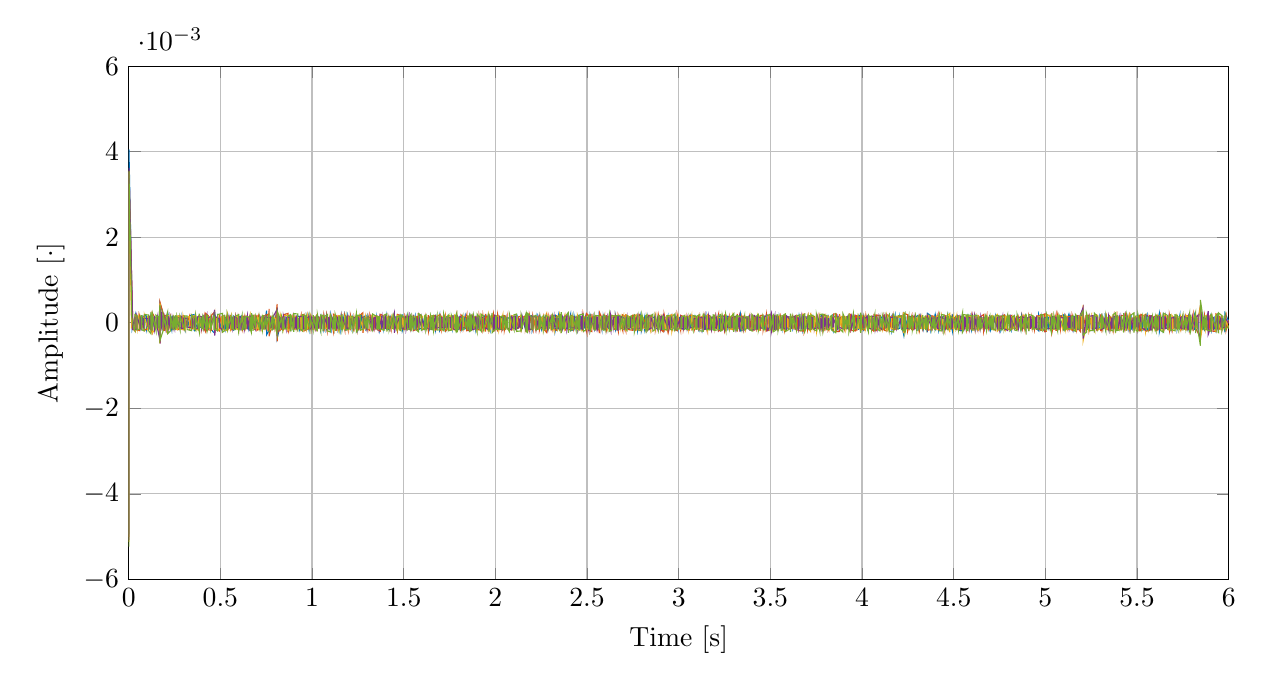
\begin{tikzpicture}

\begin{axis}[%
width=5.5in,
height=2.566in,
at={(0.758in,0.481in)},
scale only axis,
xmin=0,
xmax=6,
xlabel={Time [s]},
xmajorgrids,
ymin=-0.006,
ymax=0.006,
ylabel={Amplitude [$\cdot$]},
ymajorgrids,
axis background/.style={fill=white},
legend style={legend cell align=left,align=left,draw=white!15!black}
]
\addplot [color=mycolor1,solid]
  table[row sep=crcr]{%
2.08333333333333e-05	1.3543391321508e-05\\
0.000645833333333333	-0.00494724864934551\\
0.00125	0.00405221121651203\\
0.0195625	0.000141665120850819\\
0.0195833333333333	-0.00013070399369438\\
0.0362083333333333	0.000172035862978681\\
0.0362291666666667	-0.000173629013891336\\
0.042625	-0.000139492225705422\\
0.0426458333333333	0.000151122437035794\\
0.0675833333333333	-0.000120993218625758\\
0.0676041666666667	0.00011943275932614\\
0.0717916666666667	-0.00017310494610659\\
0.0718125	0.000175282585828263\\
0.0871875	-0.000168876734109687\\
0.0872083333333333	0.000167755613454169\\
0.0976041666666667	0.000159666556192088\\
0.097625	-0.000161031684523677\\
0.116333333333333	0.000134700280090707\\
0.116354166666667	-0.000134454739118392\\
0.127875	-0.000201213016048043\\
0.127895833333333	0.000204039027088811\\
0.139979166666667	-0.000108056527022057\\
0.14	0.000107450092484725\\
0.1641875	0.000149370296854885\\
0.164208333333333	-0.00014863602754424\\
0.170541666666667	-0.000452420246722472\\
0.1705625	0.000454140799234799\\
0.19125	0.000157341383201774\\
0.191270833333333	-0.000157032538024016\\
0.207375	-0.000113447676377216\\
0.207395833333333	0.000115914205114322\\
0.216208333333333	-0.00016723732068888\\
0.216229166666667	0.000167084370543178\\
0.233666666666667	-0.000151220774493158\\
0.2336875	0.000150785307482481\\
0.241041666666667	-0.000161900607595397\\
0.2410625	0.000162835727187046\\
0.252229166666667	-0.000138156774692538\\
0.25225	0.00013846628101136\\
0.263375	-0.000141703866857889\\
0.263395833333333	0.000143159710091053\\
0.278166666666667	0.000107540163297547\\
0.2781875	-0.00010753660409507\\
0.290958333333333	-0.000143474947561407\\
0.290979166666667	0.000144181375775723\\
0.3071875	-0.000142584604527035\\
0.307208333333333	0.000144173666773068\\
0.319708333333333	-0.000120538824343678\\
0.319729166666667	0.00012151577641364\\
0.3331875	-0.0001694180072952\\
0.333208333333333	0.000168741563561867\\
0.356625	0.00019177855321482\\
0.356645833333333	-0.000191913764764106\\
0.363125	0.000144530519561079\\
0.363145833333333	-0.000144383700601849\\
0.385604166666667	0.000103897894937403\\
0.385625	-0.00010396786149707\\
0.393520833333333	-0.000105568748329919\\
0.393541666666667	0.000104769053722883\\
0.404666666666667	-0.000133554601248609\\
0.4046875	0.0001336172365389\\
0.423583333333333	-0.000137151201648448\\
0.423604166666667	0.000138096497160287\\
0.438354166666667	0.000135715868684057\\
0.438375	-0.000134474219732723\\
0.442958333333333	0.000125206961767242\\
0.442979166666667	-0.000123970132471236\\
0.468854166666667	-0.000249132248042537\\
0.468875	0.000250025115543277\\
0.48225	-0.000117526963957053\\
0.482270833333333	0.000118233365719557\\
0.484708333333333	-0.000141046450769983\\
0.484729166666667	0.000141577590875794\\
0.505104166666667	-0.000124809065660108\\
0.505125	0.000125141413128989\\
0.516958333333333	0.00015848589030874\\
0.516979166666667	-0.000158174528732506\\
0.52875	0.000135359106418389\\
0.528770833333333	-0.000134566824710936\\
0.542645833333333	0.000107710017131189\\
0.542666666666667	-0.00010691865498761\\
0.560479166666667	0.000122069624895351\\
0.5605	-0.000121004038506202\\
0.572395833333333	0.00016905050279875\\
0.572416666666667	-0.000169554583487287\\
0.584479166666667	-0.000130861548626178\\
0.5845	0.000131328672014915\\
0.597458333333333	-0.000118703016022501\\
0.602791666666667	0.000118191454228771\\
0.613416666666667	0.000157236216477472\\
0.6134375	-0.000157042297114419\\
0.624854166666667	-0.000136019143433371\\
0.624875	0.000135703740490385\\
0.64375	0.000109909841554597\\
0.643770833333333	-0.000109362241513704\\
0.653770833333333	0.000128860167229706\\
0.653791666666667	-0.000128167508890009\\
0.6701875	0.000129076202917659\\
0.670208333333333	-0.000128824315387175\\
0.6908125	-0.000146950492514851\\
0.690833333333333	0.000147879034435434\\
0.7014375	0.000103329933575605\\
0.701458333333333	-0.000102410203119554\\
0.7076875	0.000145707371654994\\
0.707708333333333	-0.000146238251232214\\
0.725166666666667	-0.000136402563109985\\
0.7251875	0.000135913749692986\\
0.737	0.000125555172980086\\
0.737020833333333	-0.000124669181069232\\
0.752166666666667	0.000284596512112913\\
0.7521875	-0.000279696644620728\\
0.770729166666667	-0.000142196414738109\\
0.77075	0.0001420097360688\\
0.777979166666667	-0.000120621814440185\\
0.778	0.000121201758777606\\
0.792083333333333	0.000141922480351159\\
0.792104166666667	-0.000140356437681329\\
0.809854166666667	0.00036038223162328\\
0.809875	-0.000358611359133421\\
0.821854166666667	-0.000147081337702343\\
0.821875	0.000146180905360972\\
0.829958333333333	0.000131048823670882\\
0.829979166666667	-0.000131062999733082\\
0.851166666666667	0.000143417966331184\\
0.8511875	-0.000142223826653797\\
0.86275	0.000126466839338134\\
0.862770833333333	-0.000125669626614607\\
0.878041666666667	-0.000102875015222005\\
0.8780625	0.000102626009004961\\
0.894625	-0.000125406330872796\\
0.894645833333333	0.000126217923370665\\
0.903854166666667	0.000115755508684097\\
0.903875	-0.000115043740748576\\
0.916645833333333	-0.000155590535682662\\
0.916666666666667	0.000156196170556386\\
0.932645833333333	0.000149718377910048\\
0.932666666666667	-0.000149505753694775\\
0.953916666666667	0.000120368175712217\\
0.9539375	-0.000120414961167684\\
0.9539375	-0.000120414961167684\\
0.953958333333333	0.000118036703768029\\
0.969395833333333	-0.000122383170327852\\
0.969416666666667	0.000121928257076486\\
0.982375	-0.000147663940447566\\
0.982395833333333	0.000147367078271312\\
0.9968125	-0.000107533751033794\\
0.996833333333333	0.000107217917646381\\
1.01345833333333	0.000123751779292449\\
1.01347916666667	-0.000123760828078434\\
1.02333333333333	0.000122797895956282\\
1.02335416666667	-0.000122222829554891\\
1.04704166666667	0.000154114908033935\\
1.0470625	-0.000155003397872932\\
1.06339583333333	0.000130893264004194\\
1.06341666666667	-0.000130572874325926\\
1.07775	0.000152638537128504\\
1.07777083333333	-0.000151636701950249\\
1.07964583333333	-0.000125700359798761\\
1.07966666666667	0.000125595938828193\\
1.10327083333333	-0.000170125423953664\\
1.10329166666667	0.000170185007981499\\
1.11829166666667	-0.000135856169683282\\
1.1183125	0.000136902183579269\\
1.12304166666667	-0.000111818481579081\\
1.1230625	0.000111833278789776\\
1.1429375	0.000121140328024013\\
1.14295833333333	-0.000121391948619492\\
1.15754166666667	0.000167606475493034\\
1.1575625	-0.000167935115640291\\
1.17414583333333	0.000153927835146734\\
1.17416666666667	-0.000153048346421308\\
1.18370833333333	0.00017239594662089\\
1.18372916666667	-0.000171918541171765\\
1.19625	-0.000150125957420317\\
1.19627083333333	0.000150343730172517\\
1.21172916666667	-0.000115354401721551\\
1.21175	0.000116584672450018\\
1.22275	-0.000114649564212963\\
1.22277083333333	0.000114742055029859\\
1.23939583333333	-0.000118041622604156\\
1.23941666666667	0.000118029115895595\\
1.25089583333333	0.000152982851844097\\
1.25091666666667	-0.000152725294725399\\
1.26816666666667	0.00012515061780572\\
1.2681875	-0.000125006543114216\\
1.27495833333333	-0.000123569598582296\\
1.27497916666667	0.000123419449306815\\
1.29454166666667	0.000168492873743589\\
1.2945625	-0.00016817554521419\\
1.30360416666667	-0.00013276339724875\\
1.303625	0.000133995219965414\\
1.323875	0.000117698875519318\\
1.32389583333333	-0.000118040493989842\\
1.32747916666667	-0.00012473282399331\\
1.3275	0.000124402591093775\\
1.35341666666667	-0.000133269846893715\\
1.3534375	0.000133183831356034\\
1.366375	-0.000138358368083729\\
1.36639583333333	0.000139660305675579\\
1.37897916666667	-0.000140236879796835\\
1.379	0.000140552854960349\\
1.39160416666667	0.000133271896472369\\
1.391625	-0.000132782347639574\\
1.40533333333333	0.000151632219314164\\
1.40535416666667	-0.000149962418968072\\
1.41795833333333	-0.000156654773043569\\
1.41797916666667	0.000156720582568368\\
1.42797916666667	-0.000123221807260649\\
1.428	0.000124860780828232\\
1.45129166666667	-0.000135786234070089\\
1.4513125	0.000134969670086678\\
1.4649375	0.000138306307049941\\
1.46495833333333	-0.000137483254091265\\
1.47425	-0.000128793006859194\\
1.47427083333333	0.000128436964152038\\
1.48289583333333	-0.00014045864211429\\
1.48291666666667	0.000141026363699734\\
1.49322916666667	0.000176627800831061\\
1.49325	-0.000173770561561895\\
1.51689583333333	0.000160323363738404\\
1.51691666666667	-0.000158266985239212\\
1.53279166666667	-0.000136597883586854\\
1.5328125	0.000136248838526858\\
1.54158333333333	0.000148663848855512\\
1.54160416666667	-0.00014714431722911\\
1.56141666666667	0.000148912796841701\\
1.5614375	-0.000149690701693975\\
1.5723125	-0.000108287619546849\\
1.57233333333333	0.000109130970487672\\
1.58370833333333	0.000152704155745914\\
1.58372916666667	-0.000151756727548562\\
1.6026875	-0.000115428408775884\\
1.60270833333333	0.00011667794210834\\
1.61429166666667	-0.000130827894496461\\
1.6143125	0.000131363492437455\\
1.61835416666667	-0.000128773384657584\\
1.618375	0.000129258393127077\\
1.63970833333333	-0.000138062134027288\\
1.63972916666667	0.000137747123124118\\
1.65314583333333	-0.000163996465122949\\
1.65316666666667	0.000165087691122422\\
1.663	-0.000133990702488436\\
1.66302083333333	0.000135696190795926\\
1.6739375	0.000173324557187534\\
1.67395833333333	-0.000173813511036731\\
1.69610416666667	0.00018560127090805\\
1.696125	-0.000185440121132462\\
1.7045625	-0.000116467362241471\\
1.70458333333333	0.000117201798093367\\
1.72441666666667	-0.000152719324855346\\
1.7244375	0.000153098260344981\\
1.74070833333333	0.00012598067602636\\
1.74072916666667	-0.000125893396869185\\
1.74341666666667	-0.000124584780443115\\
1.7434375	0.000125783635640525\\
1.76447916666667	-0.000162689858234023\\
1.7645	0.000162863405735144\\
1.78077083333333	0.00015698805454834\\
1.78079166666667	-0.000155144582799752\\
1.79020833333333	0.000162937145527818\\
1.79022916666667	-0.000162578651643734\\
1.806125	-0.000144833208425846\\
1.80614583333333	0.000145512106895799\\
1.816625	0.000122908127625312\\
1.81664583333333	-0.000121374600831917\\
1.8341875	0.000143181022404146\\
1.83420833333333	-0.000142395949206002\\
1.84472916666667	-9.33436513852248e-05\\
1.84475	9.48548768425311e-05\\
1.863125	-0.000136247342050784\\
1.86314583333333	0.000136749690078518\\
1.87741666666667	-0.00011078034497036\\
1.8774375	0.000111562478195689\\
1.89104166666667	-0.000151655921081599\\
1.8910625	0.000153295744015116\\
1.89429166666667	-0.000146775885248086\\
1.8943125	0.000149579792013823\\
1.91747916666667	0.000131037399479026\\
1.9175	-0.000129200462035389\\
1.935125	-0.000112503616440252\\
1.93514583333333	0.000114217428646883\\
1.94004166666667	-0.000169779884479332\\
1.9400625	0.000170764660790319\\
1.9535625	-0.00011664478968796\\
1.95358333333333	0.00011758325834465\\
1.97116666666667	-0.000163881174174468\\
1.9711875	0.000165313105393781\\
1.98160416666667	-9.97120523413556e-05\\
1.981625	0.000101677859072939\\
1.99222916666667	0.000133652098428993\\
1.99225	-0.000132836765983144\\
2.01420833333333	0.000117905781565139\\
2.01422916666667	-0.000117959833987916\\
2.02302083333333	0.000153821341187556\\
2.02304166666667	-0.000151527025314206\\
2.044875	-0.000160399632028261\\
2.04489583333333	0.00016057878487074\\
2.05410416666667	0.000120226729203931\\
2.054125	-0.000118569463519222\\
2.06104166666667	-0.000107123098358097\\
2.0610625	0.000107599164523084\\
2.0809375	0.000114438331786012\\
2.08095833333333	-0.000114120950712455\\
2.09279166666667	0.000144148001587047\\
2.0928125	-0.000143406966267075\\
2.10302083333333	0.000134422411204234\\
2.10304166666667	-0.000134133634726595\\
2.12347916666667	-0.000112865238679858\\
2.1235	0.00011364451011882\\
2.13966666666667	-0.000108598047540792\\
2.1396875	0.000109700061145494\\
2.1463125	-0.000117551466362727\\
2.14633333333333	0.00011882722587117\\
2.16183333333333	-0.00011597042625328\\
2.16185416666667	0.000116671669696732\\
2.17745833333333	0.000148024704804875\\
2.17747916666667	-0.000147714689235461\\
2.18675	-0.000127914962053441\\
2.18677083333333	0.000128637013363894\\
2.20125	0.000173247800636881\\
2.20127083333333	-0.000170940516336659\\
2.22127083333333	0.000144611267731064\\
2.22129166666667	-0.000142784053520676\\
2.2324375	-0.000135265187997907\\
2.23245833333333	0.000135902933520603\\
2.25008333333333	-0.000128016442331538\\
2.25010416666667	0.000129072370290327\\
2.256	0.00013158458287971\\
2.25602083333333	-0.000131316021332153\\
2.27266666666667	-0.000142889182693695\\
2.2726875	0.000143947226860148\\
2.2905	0.000107760396599635\\
2.29052083333333	-0.000106898625786877\\
2.3033125	-0.000139318232347741\\
2.30333333333333	0.000141328815486564\\
2.30952083333333	-0.000152692059384204\\
2.30954166666667	0.000154068225574902\\
2.32685416666667	0.000177378335774913\\
2.326875	-0.000177182271540519\\
2.34295833333333	0.000148377339107539\\
2.34297916666667	-0.000147257430053195\\
2.3561875	0.000156088849770498\\
2.35620833333333	-0.000155441945379913\\
2.37385416666667	-0.000134884760070122\\
2.373875	0.000136806330851866\\
2.38270833333333	0.000146653335558451\\
2.38272916666667	-0.000145636258300762\\
2.40433333333333	-8.70644618128903e-05\\
2.40435416666667	8.82849091862917e-05\\
2.4098125	0.000186645301207788\\
2.40983333333333	-0.000184290852239901\\
2.4294375	-0.00016473225756196\\
2.42945833333333	0.000163940457421865\\
2.44522916666667	-0.000147368018084671\\
2.44525	0.000146974958046858\\
2.45077083333333	-0.000173808932910735\\
2.45079166666667	0.000175708076525538\\
2.46497916666667	0.00014539107676682\\
2.465	-0.00014468206199365\\
2.48775	-0.00011900365098633\\
2.48777083333333	0.000121299868068845\\
2.4969375	0.000140182224125689\\
2.49695833333333	-0.000139896803873611\\
2.50302083333333	-0.000131201030468578\\
2.50304166666667	0.000131417605892091\\
2.51672916666667	-0.000185173830470954\\
2.51675	0.000185874545445853\\
2.53983333333333	-0.000131406253779378\\
2.53985416666667	0.000132647718306382\\
2.55625	0.000119489215917578\\
2.55627083333333	-0.000118699173582062\\
2.5665625	-0.000140720593036016\\
2.56658333333333	0.000139667972850964\\
2.58122916666667	-0.000157894356088268\\
2.58125	0.000158305655793393\\
2.58872916666667	-0.000157275481974608\\
2.58875	0.000157428403752573\\
2.60622916666667	-0.000149360179681782\\
2.60625	0.000150384067424079\\
2.61570833333333	0.000133724177986632\\
2.61572916666667	-0.000132521566625812\\
2.62816666666667	-0.000141614369055124\\
2.6281875	0.00014307329109077\\
2.6496875	0.000111809006580983\\
2.64970833333333	-0.000111033133069155\\
2.65483333333333	-0.000169139984659741\\
2.65485416666667	0.000169326214757381\\
2.67014583333333	-0.000139965968225249\\
2.67016666666667	0.0001396216968229\\
2.68889583333333	0.00014239471776591\\
2.68891666666667	-0.000141025760314267\\
2.6965	0.000153298361805827\\
2.69652083333333	-0.000153599633231652\\
2.71647916666667	-0.000104428487657408\\
2.7165	0.000104399544535202\\
2.72520833333333	-9.06041360383078e-05\\
2.72522916666667	9.11144634149259e-05\\
2.74525	0.000113584451129902\\
2.74527083333333	-0.000113565291884959\\
2.75135416666667	-0.000150849182167715\\
2.751375	0.000152255545391053\\
2.776625	0.000160916598697674\\
2.77664583333333	-0.000160500876927395\\
2.7915625	0.000151840955466236\\
2.79158333333333	-0.000151080710626495\\
2.79729166666667	0.000168936497662456\\
2.7973125	-0.000168136175574769\\
2.81408333333333	0.000132035037409242\\
2.81410416666667	-0.000132350012713983\\
2.82641666666667	0.000126498468892451\\
2.8264375	-0.000126116234037117\\
2.83620833333333	0.000140466601291918\\
2.83622916666667	-0.000141642313718391\\
2.85785416666667	-0.000113689552639088\\
2.857875	0.000115701499825557\\
2.87164583333333	0.00014154784845293\\
2.87166666666667	-0.000140719645994471\\
2.88935416666667	-0.000125983856046464\\
2.889375	0.000126186343673086\\
2.89127083333333	-0.000120658357365867\\
2.89129166666667	0.000121677735693576\\
2.9144375	-0.000120797026096358\\
2.91445833333333	0.000120723091203068\\
2.92566666666667	0.000128243971460702\\
2.9256875	-0.000126028123266669\\
2.94025	0.000131014205914366\\
2.94027083333333	-0.000130805374168485\\
2.94779166666667	0.000134755006331461\\
2.9478125	-0.000133635760834217\\
2.96110416666667	0.000121379707099347\\
2.961125	-0.000120214753112652\\
2.98291666666667	-0.000124087258332535\\
2.9829375	0.000124126421034945\\
2.99466666666667	-0.000120401390533316\\
2.9946875	0.000121399648571162\\
3.00375	-0.000119007336275913\\
3.00408333333333	0.000119390860467511\\
3.0145625	0.000147277076403969\\
3.01458333333333	-0.000147809743967629\\
3.039375	-0.00013928490581753\\
3.03939583333333	0.00014012307344888\\
3.04747916666667	0.000128345401094246\\
3.0475	-0.000127683674321\\
3.0633125	0.000126758685058602\\
3.06333333333333	-0.000126492563078754\\
3.06935416666667	0.000114625642667628\\
3.069375	-0.000113426467527572\\
3.090875	-0.000122859443469817\\
3.09089583333333	0.000122581400808203\\
3.10910416666667	-0.000135961554724024\\
3.109125	0.00013583914788996\\
3.11079166666667	0.000131348342482493\\
3.1108125	-0.000130004884742073\\
3.13179166666667	0.000142239696838674\\
3.1318125	-0.00014097786232474\\
3.14758333333333	0.000151721835441852\\
3.14760416666667	-0.000150576731387323\\
3.15845833333333	0.000150178287969354\\
3.15847916666667	-0.000148008888541624\\
3.17029166666667	0.000119926618902801\\
3.1703125	-0.00012073932959993\\
3.1859375	-0.000144724124822377\\
3.18595833333333	0.000146364832719901\\
3.19595833333333	-0.000100365100615028\\
3.19597916666667	0.000101763629540707\\
3.219	0.000161089052589765\\
3.21902083333333	-0.000160845358749914\\
3.22120833333333	0.000152723964637986\\
3.22122916666667	-0.000145576289109323\\
3.23575	-0.000169431958343427\\
3.23577083333333	0.00016844634324123\\
3.25785416666667	0.000128977706358096\\
3.257875	-0.000129300399085932\\
3.26429166666667	-0.000156181043860077\\
3.2643125	0.000155118258309142\\
3.27758333333333	0.000122627702440383\\
3.27760416666667	-0.000122047617098432\\
3.2935625	0.000116010426939143\\
3.29358333333333	-0.000114542851250845\\
3.30991666666667	-0.000114328162385214\\
3.3099375	0.000114366609196913\\
3.31829166666667	0.000123007652193185\\
3.3183125	-0.000124091584339474\\
3.33616666666667	0.000194110791369092\\
3.3361875	-0.000192361738502165\\
3.3560625	-0.000161286020934765\\
3.35608333333333	0.000161333124571981\\
3.364875	-0.000142679236291246\\
3.36489583333333	0.00014313134293271\\
3.384125	0.000105860622878799\\
3.38414583333333	-0.000105445458814905\\
3.39625	-9.59145242049673e-05\\
3.39627083333333	9.57936467221202e-05\\
3.41016666666667	0.000118597883191141\\
3.4101875	-0.000119326127109098\\
3.4213125	0.000154920231681413\\
3.42133333333333	-0.000154265394012556\\
3.43947916666667	-0.000127520091916042\\
3.4395	0.000126502217892818\\
3.44964583333333	0.000110234632675145\\
3.44966666666667	-0.000109711729675628\\
3.46597916666667	-0.000158652962792743\\
3.466	0.000158246390078754\\
3.47054166666667	0.000151789227660419\\
3.4705625	-0.000151084165462056\\
3.49491666666667	-0.000103530605207859\\
3.4949375	0.000105333730321353\\
3.50522916666667	0.000138778349143044\\
3.50845833333333	-0.000138203578862052\\
3.5194375	-0.000158403593602751\\
3.51945833333333	0.000158769428164352\\
3.53114583333333	0.000147452127725699\\
3.53116666666667	-0.000147390509515388\\
3.54927083333333	-0.000130861807270052\\
3.54929166666667	0.000129859078545145\\
3.5625	-0.000125593408333506\\
3.56252083333333	0.0001256796900086\\
3.5723125	0.000126060923950238\\
3.57233333333333	-0.000126938202424011\\
3.5865	-0.000160528288788089\\
3.58652083333333	0.000160765830785872\\
3.595625	-0.000143577108426866\\
3.59564583333333	0.000144649194640591\\
3.61972916666667	0.000123607212566944\\
3.61975	-0.000122761703425244\\
3.6230625	0.000142848326927458\\
3.62308333333333	-0.000143542685157505\\
3.64885416666667	0.000141101026806346\\
3.648875	-0.000141559467765317\\
3.65910416666667	-0.000119766362991673\\
3.659125	0.000121073636573571\\
3.6725	-0.000144495315075023\\
3.67252083333333	0.000143556695341646\\
3.6811875	-0.000139081921023623\\
3.68120833333333	0.000139132480209284\\
3.7035625	9.17716169842344e-05\\
3.70358333333333	-9.05981870362211e-05\\
3.70552083333333	0.0001427361845094\\
3.70554166666667	-0.000141829762661125\\
3.7298125	0.000134043123122778\\
3.72983333333333	-0.000134782419054206\\
3.74220833333333	0.000144200209607004\\
3.74222916666667	-0.000143874089286997\\
3.75347916666667	0.000131933037848065\\
3.7535	-0.000131026973148009\\
3.77377083333333	-0.000149308156603625\\
3.77379166666667	0.000149338133261457\\
3.78302083333333	0.000183146294805413\\
3.78304166666667	-0.000182191173964044\\
3.79885416666667	-0.000122896544820043\\
3.798875	0.000122553807658117\\
3.804625	-0.000134089494135554\\
3.80464583333333	0.000134093093154418\\
3.81670833333333	-0.000132483635625449\\
3.81672916666667	0.000131989580439904\\
3.84154166666667	-0.000178013585275555\\
3.8415625	0.000176849532769052\\
3.85652083333333	0.000120042669500739\\
3.85654166666667	-0.000120208322069194\\
3.86535416666667	0.000146705770877943\\
3.865375	-0.000147774790300695\\
3.87760416666667	-0.000122065013405774\\
3.877625	0.000122040753078526\\
3.89672916666667	0.000126078863228034\\
3.89675	-0.000125453200580551\\
3.91141666666667	-0.00012765419427618\\
3.9114375	0.000129090572147601\\
3.92041666666667	-0.000150790345972472\\
3.9204375	0.000151995581727287\\
3.93097916666667	-0.000106264023131088\\
3.94010416666667	0.000109793045166727\\
3.94595833333333	-0.000133147035331888\\
3.94597916666667	0.000132751848613572\\
3.95441666666667	0.000157811668414909\\
3.9544375	-0.000157791374535482\\
3.9815625	0.000147152261140466\\
3.98158333333333	-0.000157007225978537\\
3.981625	-0.000167652133118065\\
3.98164583333333	0.000168386720354613\\
4.00752083333333	0.000169000396441035\\
4.00754166666667	-0.000168550947033449\\
4.0111875	-0.000140017531333231\\
4.01120833333333	0.000139423940568779\\
4.03252083333333	0.000161849104690453\\
4.03254166666667	-0.000160833646484953\\
4.04160416666667	-0.000109768294251504\\
4.041625	0.000109187327079171\\
4.06108333333333	-0.000114548818386216\\
4.06110416666667	0.000115198550177858\\
4.06954166666667	0.000158218094152615\\
4.0695625	-0.000158068104707079\\
4.07835416666667	0.000128252555991989\\
4.08233333333333	-0.000123933500342595\\
4.10358333333333	-0.000133541471848733\\
4.10360416666667	0.000134333393726818\\
4.11222916666667	0.00012109407378239\\
4.11225	-0.000121133207615548\\
4.1314375	0.000131758781847001\\
4.13145833333333	-0.000131299799099952\\
4.1386875	0.0001223263072734\\
4.13870833333333	-0.000123111752433082\\
4.15508333333333	-9.04054718471975e-05\\
4.15510416666667	9.12397154573975e-05\\
4.16339583333333	0.000165733249223232\\
4.16341666666667	-0.00016556886109426\\
4.17975	0.000152990240342523\\
4.17977083333333	-0.000152428589200778\\
4.19185416666667	0.00014006539002278\\
4.191875	-0.000138295540501098\\
4.20658333333333	-0.000129887688685519\\
4.20660416666667	0.000129780013328007\\
4.22591666666667	-0.000254218888925929\\
4.2259375	0.000254693104498953\\
4.23310416666667	-0.000139744848484085\\
4.233125	0.000139587557674413\\
4.245875	-0.000135632876204083\\
4.24589583333333	0.000135005033289222\\
4.2698125	0.000149483439820682\\
4.26983333333333	-0.000149249595124696\\
4.27797916666667	0.000130561095794592\\
4.278	-0.000130904738642842\\
4.29308333333333	-0.000137682274004655\\
4.29310416666667	0.000137530161886059\\
4.30475	0.000170660938315617\\
4.30477083333333	-0.000172285856860313\\
4.31960416666667	-0.000126494138407141\\
4.319625	0.000126588306383314\\
4.33429166666667	-0.000123160993589649\\
4.3343125	0.000122095170444878\\
4.34377083333333	-0.000109695680615512\\
4.34379166666667	0.00010864142169403\\
4.35641666666667	-0.000220743619476821\\
4.3564375	0.00022014338567494\\
4.376125	0.000161602569223756\\
4.37614583333333	-0.000160766724214067\\
4.3939375	0.000119779959050906\\
4.39395833333333	-0.000121004239808307\\
4.40097916666667	-0.00016035198716727\\
4.401	0.000160440501168205\\
4.41554166666667	-0.000135841617681743\\
4.4155625	0.000134986596094059\\
4.43775	-0.000135528770056254\\
4.43777083333333	0.000135593425347823\\
4.44933333333333	0.000154818844011449\\
4.44935416666667	-0.000155458091637072\\
4.46427083333333	0.000140561448645425\\
4.46429166666667	-0.000141997887296786\\
4.47685416666667	-0.000133194979284394\\
4.476875	0.000132282538600013\\
4.49254166666667	-0.000184059513813481\\
4.4925625	0.000184693401091459\\
4.49610416666667	0.000173416705724978\\
4.496125	-0.000173877027294996\\
4.5184375	0.000120485098238464\\
4.51845833333333	-0.000120944923961948\\
4.52535416666667	0.000168524515353112\\
4.525375	-0.000169373821499661\\
4.54733333333333	-0.000189472176381595\\
4.54735416666667	0.00018998532782351\\
4.54904166666667	-0.000127906578512271\\
4.5490625	0.000127306985252808\\
4.566875	0.000127824453515136\\
4.56689583333333	-0.000129093679387466\\
4.58029166666667	-0.000123752224942439\\
4.5803125	0.000122527232823547\\
4.59560416666667	-0.000143471132672692\\
4.595625	0.000143586423539565\\
4.61660416666667	-0.000150107664871282\\
4.616625	0.000149748461112006\\
4.61797916666667	-0.000146438361841706\\
4.618	0.000146598990047154\\
4.635625	-0.000117446105109449\\
4.63564583333333	0.0001178481670296\\
4.65683333333333	0.000110587703749959\\
4.65685416666667	-0.000111279731095313\\
4.67077083333333	-0.000108247848204461\\
4.67079166666667	0.000107445440486284\\
4.67364583333333	-0.000119787956966682\\
4.67366666666667	0.000118499346898262\\
4.6966875	-0.000161410990066708\\
4.69670833333333	0.000160771690645237\\
4.703875	0.000134958647802739\\
4.70389583333333	-0.000134297441749307\\
4.727625	0.00016484931011774\\
4.72764583333333	-0.000163930374834961\\
4.74166666666667	0.000151003224286052\\
4.7416875	-0.000152574800349341\\
4.74625	0.000116269291674273\\
4.74627083333333	-0.000115795936175849\\
4.75822916666667	0.000169514506076936\\
4.75825	-0.000169304276658546\\
4.78133333333333	0.000117770374185384\\
4.78135416666667	-0.000118128530468755\\
4.7888125	-0.00010264515037427\\
4.78883333333333	0.000101996085383453\\
4.80954166666667	0.00013334300411608\\
4.8095625	-0.000134037536266371\\
4.8125625	-0.000167953897822665\\
4.81258333333333	0.000167290823819361\\
4.8254375	0.000126281859835647\\
4.82545833333333	-0.000126811703264944\\
4.8484375	-0.000131805038022076\\
4.84845833333333	0.000132120473194062\\
4.86525	-0.000144849367054208\\
4.86527083333333	0.000144007523206491\\
4.87072916666667	-0.000175889768839082\\
4.87075	0.000174594942093833\\
4.8931875	-0.000132022097098765\\
4.89320833333333	0.000131686319910472\\
4.8943125	-0.000121898781618749\\
4.89433333333333	0.000120306593047383\\
4.90829166666667	-0.000108442323736696\\
4.9083125	0.000107623963743331\\
4.92897916666667	0.000115731902761946\\
4.929	-0.000115219617173806\\
4.93814583333333	0.000148525286762621\\
4.93816666666667	-0.000150496011625401\\
4.95066666666667	0.000131748333011209\\
4.9506875	-0.000131714825159173\\
4.96404166666667	-0.000189536400651141\\
4.9640625	0.000189673872562601\\
4.98664583333333	-0.000115333243447457\\
4.98666666666667	0.000115159832521808\\
4.99666666666667	-0.000121678999128823\\
4.9966875	0.000121084003789907\\
5.01758333333333	-0.000128728212328708\\
5.01760416666667	0.000128857131487052\\
5.031	0.00014253087321492\\
5.03102083333333	-0.000143566598881659\\
5.04389583333333	0.000137017669698241\\
5.04391666666667	-0.000137104921039086\\
5.05516666666667	-0.000140919590864748\\
5.0551875	0.000140893607821723\\
5.0631875	0.000131777581654229\\
5.06320833333333	-0.000133033993474342\\
5.07725	-0.000141260381431703\\
5.07727083333333	0.000140967132443696\\
5.09902083333333	0.0001842786627429\\
5.09904166666667	-0.000184309885395694\\
5.10945833333333	0.000113265646802189\\
5.10947916666667	-0.000113557341943487\\
5.12322916666667	0.000116026864718588\\
5.12325	-0.000115482879507453\\
5.1316875	-0.000152568029635838\\
5.13170833333333	0.000151534529986035\\
5.1485625	-0.000140961612841778\\
5.14858333333333	0.000138865343178062\\
5.15889583333333	0.000147758424731193\\
5.15891666666667	-0.00014806287642389\\
5.18097916666667	0.00011664887587111\\
5.181	-0.000117615435947078\\
5.19060416666667	-0.000128370234235778\\
5.190625	0.000128733377280759\\
5.20625	0.00024079827344836\\
5.20627083333333	-0.000241585800953761\\
5.22035416666667	-0.000129101427952791\\
5.220375	0.000129856914048188\\
5.22758333333333	0.000149743833873648\\
5.22760416666667	-0.000155111725971337\\
5.24045833333333	-0.00011293435477983\\
5.24047916666667	0.000112917473655516\\
5.258125	-0.000142189867050251\\
5.25814583333333	0.000141227943143531\\
5.27139583333333	-0.000143042820270432\\
5.27141666666667	0.000142754832476385\\
5.282	0.00014734016291886\\
5.28202083333333	-0.000148395216437289\\
5.2980625	-0.000115213883635367\\
5.29808333333333	0.000114687457175691\\
5.3115	-0.000116754792748465\\
5.31152083333333	0.000116809333067014\\
5.326875	-0.000135418483627584\\
5.32689583333333	0.000134449705869988\\
5.34320833333333	-0.000107488301666206\\
5.34322916666667	0.000106863840746035\\
5.35139583333333	-0.00010928755328947\\
5.35141666666667	0.000110088435072509\\
5.37427083333333	0.000129914327595595\\
5.37429166666667	-0.00013037371428442\\
5.3789375	0.000124562378496559\\
5.37895833333333	-0.000124634363199919\\
5.40445833333333	-0.000147953580117588\\
5.40447916666667	0.000147492431305207\\
5.4091875	0.000120773147669611\\
5.40920833333333	-0.000120394019480835\\
5.430375	-0.000147747344774361\\
5.43039583333333	0.000147087178003389\\
5.44089583333333	-0.000146153333373154\\
5.44091666666667	0.00014662722479147\\
5.45408333333333	-0.000129720711325946\\
5.45410416666667	0.000130304746970715\\
5.4675	0.000167052128980321\\
5.46752083333333	-0.000166220544548697\\
5.47908333333333	0.000118645299422078\\
5.47910416666667	-0.000117957993426951\\
5.49941666666667	0.000136154990928609\\
5.4994375	-0.000137071896521241\\
5.5045	-0.000157644561743258\\
5.50452083333333	0.000158260750226032\\
5.52689583333333	-0.000121481250884087\\
5.52691666666667	0.000125647189031928\\
5.53108333333333	0.000115873944524568\\
5.53110416666667	-0.000113932070417018\\
5.5545	0.000176945343264873\\
5.55452083333333	-0.000176811174115479\\
5.56360416666667	-0.000135739481144817\\
5.563625	0.000136678535675054\\
5.57516666666667	0.000155043727774456\\
5.5751875	-0.000155378003364398\\
5.58552083333333	-0.000108382092616802\\
5.59602083333333	0.000107724125975602\\
5.60166666666667	0.000110259378180111\\
5.6016875	-0.000110790121891446\\
5.62160416666667	0.00021570891098724\\
5.621625	-0.000215451476454422\\
5.639375	0.000132934280411366\\
5.63939583333333	-0.000133233526044612\\
5.65339583333333	0.000141684334558627\\
5.65341666666667	-0.000141285284216634\\
5.66395833333333	0.000130686764394036\\
5.66397916666667	-0.0001301344329181\\
5.67454166666667	-0.000152847199022909\\
5.6745625	0.000152792769920086\\
5.68422916666667	0.000158958358826067\\
5.68425	-0.000158508506139272\\
5.699875	-0.00013437748199803\\
5.69989583333333	0.000134746917880904\\
5.71895833333333	0.000132091227196907\\
5.71897916666667	-0.000132725765300563\\
5.73302083333333	0.000160402451018637\\
5.73304166666667	-0.000160625118785808\\
5.74254166666667	0.000132762922971718\\
5.7425625	-0.000133225915101785\\
5.75783333333333	-0.00013319782538985\\
5.75785416666667	0.000133323705122377\\
5.77602083333333	-0.000142662831508294\\
5.77604166666667	0.00014382093509412\\
5.77960416666667	0.000161580899952796\\
5.779625	-0.000161341129366079\\
5.8039375	-0.000122351811066135\\
5.80395833333333	0.000120851854725519\\
5.81454166666667	-0.000168280153018247\\
5.8145625	0.000167937904226454\\
5.83275	-0.000105175723590821\\
5.83277083333333	0.000105635577482316\\
5.8455	0.000323676818798491\\
5.84552083333333	-0.000323737631054314\\
5.8601875	0.00012410764696928\\
5.86020833333333	-0.000123931770251202\\
5.86704166666667	-0.000166957936848744\\
5.8670625	0.000166332586784782\\
5.88822916666667	-0.000172619012439112\\
5.88825	0.000172046392513774\\
5.8924375	-0.000119313561365742\\
5.89245833333333	0.000119181585744558\\
5.90472916666667	-0.000133667739364963\\
5.90475	0.000133881055484354\\
5.92429166666667	-0.000151544715298856\\
5.9243125	0.000151034994131383\\
5.93627083333333	-0.000123041860948903\\
5.93629166666667	0.0001234251131987\\
5.94677083333333	0.000136323882204421\\
5.94679166666667	-0.000137024381675308\\
5.9671875	-0.000154263459081055\\
5.96720833333333	0.000153107197360926\\
5.979625	-0.000220815726645522\\
5.97964583333333	0.000220733104255833\\
6	4.08992316518733e-05\\
};
%\addlegendentry{Test1};

\addplot [color=mycolor2,solid]
  table[row sep=crcr]{%
2.08333333333333e-05	0.000211652413002886\\
0.000645833333333333	-0.00500716086243622\\
0.00125	0.00356456277667745\\
0.0209375	0.000167143283527687\\
0.0259791666666667	-0.000158174211819175\\
0.0364375	-0.000199406866236328\\
0.0364583333333333	0.000191149822190383\\
0.0434375	0.000162773258465628\\
0.0434583333333333	-0.000155710056128073\\
0.0576666666666667	-0.000182265281448289\\
0.0576875	0.000183125414054308\\
0.0789791666666667	-0.000126865117002039\\
0.079	0.00013054408406375\\
0.0866875	0.00018162060183318\\
0.0867083333333333	-0.000180179849932869\\
0.104104166666667	-0.000128472019282181\\
0.104125	0.000131244217481765\\
0.120791666666667	0.000163799642589153\\
0.1208125	-0.000160179059129618\\
0.127875	-0.00023172128676707\\
0.127895833333333	0.000235079930728156\\
0.1390625	0.000150477820232021\\
0.139083333333333	-0.000148980213640632\\
0.152458333333333	-0.000103637714005109\\
0.165395833333333	0.000105039266392407\\
0.1705	-0.000484540456671894\\
0.170520833333333	0.000482462346584361\\
0.190645833333333	0.000179290038383443\\
0.190666666666667	-0.000176497198677262\\
0.193875	-0.000175216795568742\\
0.193895833333333	0.000178804206533869\\
0.209020833333333	0.000151340408700463\\
0.209041666666667	-0.000149556691288206\\
0.226375	0.000124641265415688\\
0.226395833333333	-0.000123150888616338\\
0.244333333333333	-0.000118666202398059\\
0.244354166666667	0.000120525969048638\\
0.258208333333333	0.000131864243055923\\
0.258229166666667	-0.000130878395166813\\
0.273291666666667	-0.000160519233225676\\
0.2733125	0.000162642206643962\\
0.2873125	0.000151939510903251\\
0.287333333333333	-0.000150380000699482\\
0.297541666666667	0.000178025642284342\\
0.2975625	-0.000176841568438442\\
0.304583333333333	0.000127903293454055\\
0.304604166666667	-0.000127749793893068\\
0.331520833333333	0.000159999276158185\\
0.331541666666667	-0.000160738744007252\\
0.343354166666667	0.00013642675970928\\
0.343375	-0.000135866386095161\\
0.348479166666667	-0.000141747260370758\\
0.3485	0.000143803932405563\\
0.363166666666667	0.000159145781469516\\
0.3631875	-0.000158915308197381\\
0.383416666666667	-0.000161115732829748\\
0.3834375	0.000163701531308037\\
0.398104166666667	0.000133326039249037\\
0.398125	-0.00013172195574493\\
0.411520833333333	0.000146658160024867\\
0.411541666666667	-0.000145117359389815\\
0.419854166666667	-0.000214707767857129\\
0.419875	0.000218094419223937\\
0.434854166666667	0.000163300574398163\\
0.434875	-0.000164709511063595\\
0.452229166666667	-0.000177167562179492\\
0.45225	0.000179462177144493\\
0.468916666666667	0.000252920798134792\\
0.4689375	-0.000248559039934471\\
0.477270833333333	0.000134752178572451\\
0.477291666666667	-0.000132261727690598\\
0.494708333333333	-0.000191957684960549\\
0.494729166666667	0.00019250648060885\\
0.511520833333333	-0.000169689584303799\\
0.511541666666667	0.000169562114398005\\
0.511541666666667	0.000169562114398005\\
0.5115625	-0.000163216072495621\\
0.536395833333333	0.000178262764594929\\
0.536416666666667	-0.000177822565433984\\
0.541791666666667	0.000174421414954934\\
0.5418125	-0.000173282788138084\\
0.554625	0.000175945305822464\\
0.554645833333333	-0.00017563082888888\\
0.574	-0.000135061437584401\\
0.574020833333333	0.000136615752932303\\
0.585229166666667	-0.000123824909398349\\
0.58525	0.00012521422098207\\
0.598708333333333	-0.00014336088842771\\
0.598729166666667	0.000146796885923763\\
0.620583333333333	-0.000164058539949367\\
0.620604166666667	0.0001660078559021\\
0.6223125	-0.000152124222179678\\
0.622333333333333	0.000152258133966261\\
0.644895833333333	0.000151045145744693\\
0.644916666666667	-0.00014738988517042\\
0.658	0.000147487878694759\\
0.658020833333333	-0.000145920622909806\\
0.670583333333333	-0.000136107962726869\\
0.670604166666667	0.000140000548894909\\
0.683916666666667	0.000174039867979886\\
0.6839375	-0.00017133549092354\\
0.699604166666667	0.000182460400215573\\
0.699625	-0.000179281468471519\\
0.708791666666667	-0.000146448831854107\\
0.7088125	0.000148921052388554\\
0.729166666666667	-0.000127762812794793\\
0.7291875	0.000130007093819705\\
0.7348125	-0.000148908972832581\\
0.734833333333333	0.00015156413171327\\
0.759458333333333	0.000196440402715915\\
0.759479166666667	-0.000194529870897583\\
0.7660625	0.00032217710041116\\
0.766083333333333	-0.000315352359842922\\
0.77425	0.00016381228278605\\
0.774270833333333	-0.000159975424921258\\
0.788729166666667	0.000121296473662111\\
0.796791666666667	-0.000121344320417457\\
0.8098125	0.000437734195292456\\
0.809833333333333	-0.000432999271735739\\
0.8189375	0.000193941110718257\\
0.818958333333333	-0.000193614424947332\\
0.8355	-0.00014496960807313\\
0.835520833333333	0.000147289204686998\\
0.8438125	-0.000184304249748057\\
0.843833333333333	0.000185272647450027\\
0.869041666666667	0.000219586814700484\\
0.8690625	-0.000217217007392246\\
0.872833333333333	0.000175636393026647\\
0.872854166666667	-0.000174262199930902\\
0.891145833333333	0.000121025508358958\\
0.891166666666667	-0.000120389767334701\\
0.906916666666667	-0.000153700215621497\\
0.9069375	0.000156507026986932\\
0.919729166666667	0.000144490998899209\\
0.91975	-0.000143042182498019\\
0.939791666666667	0.000172486188589379\\
0.9398125	-0.000171519319412658\\
0.943083333333333	-0.000155802628353773\\
0.943104166666667	0.000156214309761955\\
0.9559375	0.000193562305256922\\
0.955958333333333	-0.000192478034751118\\
0.979104166666667	-0.000143014629185481\\
0.979125	0.000144644517402046\\
0.993354166666667	-0.000142173219915484\\
0.993375	0.00014291851988532\\
1.00577083333333	-0.000163532500163633\\
1.00579166666667	0.000164606212039325\\
1.0185625	-0.000109982975304129\\
1.01858333333333	0.000112650825667216\\
1.02710416666667	-0.000201133241964604\\
1.027125	0.000200398980366533\\
1.04102083333333	-0.000123360961497176\\
1.04104166666667	0.000123779579766129\\
1.06233333333333	0.000147956420387031\\
1.06235416666667	-0.000147468540412929\\
1.06495833333333	-0.000164996734255597\\
1.06497916666667	0.000168554983799797\\
1.08158333333333	-0.000177549642359946\\
1.08160416666667	0.000178782192920006\\
1.0996875	-0.000140297828831456\\
1.09970833333333	0.000142550405665477\\
1.11622916666667	-0.000198264379455396\\
1.11625	0.000199520288032844\\
1.12808333333333	0.000159005811404847\\
1.12810416666667	-0.00015802120391274\\
1.13504166666667	-0.00017926818017306\\
1.1350625	0.000182033365039382\\
1.15054166666667	-0.000174520925598251\\
1.1505625	0.000174979233626148\\
1.163125	-0.00014359372031339\\
1.16314583333333	0.000145432263426419\\
1.17820833333333	-0.000158380238793338\\
1.17822916666667	0.000160431713368766\\
1.1963125	-0.000167232283552158\\
1.19633333333333	0.000168865770442173\\
1.20914583333333	-0.000174885929324748\\
1.20916666666667	0.000175512750542091\\
1.22527083333333	-0.000131444391056693\\
1.22904166666667	0.00013354906700883\\
1.24408333333333	-0.000166197584049604\\
1.24410416666667	0.000167598835210252\\
1.25220833333333	-0.000180319468981053\\
1.25222916666667	0.000179711328348276\\
1.2628125	-0.000174552773886375\\
1.26283333333333	0.000177206961929042\\
1.277625	0.000236880547128089\\
1.27764583333333	-0.00023671271763452\\
1.29004166666667	0.000148141892345393\\
1.2900625	-0.000148046868907556\\
1.30154166666667	0.000142589945725794\\
1.3015625	-0.000142430633847482\\
1.3155	-0.000183280577816958\\
1.31552083333333	0.000184290290952124\\
1.33654166666667	-0.00013047542663591\\
1.3365625	0.00013119406386209\\
1.343125	-0.000159098278947092\\
1.34314583333333	0.000160633352872545\\
1.35529166666667	0.000158703451490715\\
1.3553125	-0.000158208163457347\\
1.37208333333333	-0.000196807830513285\\
1.37210416666667	0.000198176984059698\\
1.38770833333333	0.000169035096872671\\
1.38772916666667	-0.00016736368453442\\
1.40008333333333	0.000123426629016911\\
1.4063125	-0.000123086232172087\\
1.41622916666667	-0.000134576109070003\\
1.41625	0.000135455373675427\\
1.4314375	-0.000149702657409409\\
1.43145833333333	0.000150683169052541\\
1.44322916666667	-0.000126217530697533\\
1.44325	0.000126796063718845\\
1.465	-0.000187309016130515\\
1.46502083333333	0.00018761548866824\\
1.46691666666667	-0.000193139070942982\\
1.4669375	0.000194140688975637\\
1.4821875	0.000163208799221727\\
1.48220833333333	-0.000163195395323752\\
1.49725	0.000159104647402568\\
1.49727083333333	-0.000158637662803918\\
1.50714583333333	-0.000159954728234341\\
1.50716666666667	0.000161137007378327\\
1.53404166666667	-0.000148411964296505\\
1.5340625	0.000150119149310478\\
1.53908333333333	0.000166344289731809\\
1.53910416666667	-0.000164622558612307\\
1.553375	0.000182183183586017\\
1.55339583333333	-0.00018090955456179\\
1.570875	-0.000158834202760515\\
1.57089583333333	0.000158782916128199\\
1.57941666666667	-0.000196661734581716\\
1.5794375	0.000198550492586005\\
1.59847916666667	0.000138972792025242\\
1.5985	-0.000138726823205178\\
1.61375	-0.000136662464714747\\
1.61377083333333	0.000137250597663307\\
1.6191875	-0.000125313076397123\\
1.61920833333333	0.000124683537981328\\
1.63389583333333	-0.000178430942239469\\
1.63391666666667	0.000178101105391653\\
1.64672916666667	-0.000149339695183619\\
1.64675	0.000150938758997878\\
1.67172916666667	0.00017159030676531\\
1.67175	-0.000173210020388795\\
1.680375	-0.000139759839599567\\
1.68039583333333	0.000139895740992729\\
1.69866666666667	0.000196808362424095\\
1.6986875	-0.00019644608695618\\
1.70797916666667	0.000166849524735344\\
1.708	-0.000166309678804959\\
1.72725	0.000164842571573451\\
1.72727083333333	-0.000165147377511038\\
1.72866666666667	0.000192239134544914\\
1.7286875	-0.000192626457599043\\
1.7434375	-0.000136396329167487\\
1.75579166666667	0.000137258788717772\\
1.76683333333333	0.000151491946524863\\
1.76685416666667	-0.000149569350394034\\
1.7754375	-0.000132490980552926\\
1.77545833333333	0.000133790094222666\\
1.79014583333333	-0.000177896502225356\\
1.79016666666667	0.000180000166294684\\
1.80654166666667	-0.000137481727894446\\
1.8065625	0.000137466631089426\\
1.81172916666667	-0.000186659718202101\\
1.81175	0.000186278903226503\\
1.82552083333333	0.000132566655207353\\
1.82554166666667	-0.000133025330577773\\
1.84410416666667	0.000186775169530193\\
1.844125	-0.000185806224357665\\
1.86589583333333	-0.000162722708306004\\
1.86591666666667	0.000165874126492394\\
1.87175	-0.000188897137828825\\
1.87177083333333	0.000191101932580422\\
1.88525	-0.000134330642574909\\
1.88527083333333	0.000134554127183684\\
1.8994375	0.000147312355773863\\
1.89945833333333	-0.000147489135336203\\
1.911	-0.000167805901210903\\
1.91102083333333	0.000170490922749741\\
1.92754166666667	-0.000169987978148952\\
1.93225	0.000171560048160086\\
1.94589583333333	-0.000207852226900411\\
1.94591666666667	0.000208702043579845\\
1.95179166666667	-0.000143636684516675\\
1.9518125	0.000146299122235075\\
1.96660416666667	0.000163646855145344\\
1.966625	-0.00016112506397434\\
1.98829166666667	0.000202584827014205\\
1.9883125	-0.000199587659785411\\
1.99716666666667	-0.000184668173976737\\
1.9971875	0.000187310165074054\\
2.01191666666667	-0.000204200950535969\\
2.0119375	0.000203598248268984\\
2.0313125	-0.000145718991628308\\
2.03133333333333	0.00014613794576526\\
2.03658333333333	-0.000154926341040796\\
2.03660416666667	0.000157760818286815\\
2.04947916666667	0.000167149183808919\\
2.0495	-0.00016726364572451\\
2.0643125	0.000142827815113953\\
2.06433333333333	-0.000140980078496958\\
2.08704166666667	-0.000168466692095396\\
2.0870625	0.000171208351297499\\
2.08972916666667	-0.000113118267398357\\
2.08975	0.000114995588103917\\
2.1125625	-0.000152515532235255\\
2.11258333333333	0.000152306879052708\\
2.1261875	-0.000138805611195342\\
2.12620833333333	0.000139550576626143\\
2.14247916666667	0.000156874477743675\\
2.1425	-0.00015607496403556\\
2.14420833333333	-0.000132470301492667\\
2.152	0.000132020268017553\\
2.16358333333333	0.000161610709116631\\
2.16360416666667	-0.000164184837327287\\
2.18154166666667	0.000139330268736576\\
2.1815625	-0.000140723959478299\\
2.186125	-0.000183200533992565\\
2.18614583333333	0.000182099826022627\\
2.2050625	-0.000148263854129958\\
2.20508333333333	0.000147710708685167\\
2.21895833333333	-0.00013433433761029\\
2.21897916666667	0.000135119542564445\\
2.22752083333333	0.000140791577757274\\
2.22754166666667	-0.000140774197181333\\
2.23997916666667	0.000186873887238915\\
2.24	-0.000184840700055334\\
2.261625	0.000140388632622705\\
2.26164583333333	-0.000138522887835829\\
2.27904166666667	-0.000225115952154675\\
2.2790625	0.000227634518303723\\
2.292	-0.000146883947014981\\
2.29202083333333	0.000146766931623077\\
2.30858333333333	-0.000137498471388312\\
2.30860416666667	0.000136759122241359\\
2.30922916666667	0.000129637853434375\\
2.30925	-0.000128913936645485\\
2.33483333333333	-0.000180347964064958\\
2.33485416666667	0.000179594393079001\\
2.34958333333333	-0.000173039806438503\\
2.34960416666667	0.000171933747270149\\
2.358875	0.000157343017396399\\
2.35889583333333	-0.000156399156339733\\
2.37760416666667	0.000144018037990775\\
2.377625	-0.000144245527591196\\
2.38264583333333	-0.000166299937459613\\
2.38266666666667	0.000165422379203496\\
2.39679166666667	0.000157541999939728\\
2.3968125	-0.000156865460984864\\
2.41625	-0.00016458575703139\\
2.41627083333333	0.000165694216120032\\
2.42695833333333	0.000137676447312513\\
2.42697916666667	-0.000139802710793253\\
2.44577083333333	0.000127079162083801\\
2.44579166666667	-0.000127204486631749\\
2.45166666666667	0.000164791771827507\\
2.4516875	-0.0001657607274919\\
2.47289583333333	0.000145148336446259\\
2.47291666666667	-0.000145414495015299\\
2.4793125	-0.000188262012419489\\
2.47933333333333	0.000189738847028481\\
2.49866666666667	-0.000214721466480321\\
2.4986875	0.000213644961863328\\
2.50829166666667	0.000172952950563923\\
2.5083125	-0.000172345150864794\\
2.52625	-0.000205676308519438\\
2.52627083333333	0.000205568289080995\\
2.53777083333333	-0.000151103063930184\\
2.53779166666667	0.000150901473488262\\
2.551	-0.000151050407905282\\
2.55102083333333	0.000150162127961839\\
2.56766666666667	-0.000243378961611586\\
2.5676875	0.000243336386347309\\
2.57654166666667	0.000162176628405145\\
2.5765625	-0.000161057566037888\\
2.5953125	0.000158059694810399\\
2.59533333333333	-0.00015758367023022\\
2.60554166666667	0.000176060439500029\\
2.6055625	-0.000173501335859959\\
2.62216666666667	0.000143539725736511\\
2.6221875	-0.000143325841697483\\
2.63077083333333	-0.000178738370765658\\
2.63079166666667	0.000176304684394777\\
2.64822916666667	0.000152536135044008\\
2.64825	-0.000152242518625929\\
2.65441666666667	-0.000155947816625159\\
2.6544375	0.000155650292587372\\
2.6700625	-0.000173927147060732\\
2.67008333333333	0.00017350100773808\\
2.69464583333333	-0.000184155092081984\\
2.69466666666667	0.00018248292617499\\
2.708875	0.000144695645496028\\
2.70889583333333	-0.000144472756239669\\
2.71127083333333	-0.000182564266883675\\
2.71129166666667	0.000182391547311344\\
2.723625	0.000157383763044083\\
2.72364583333333	-0.000158480423316162\\
2.74916666666667	-0.000176135311749006\\
2.7491875	0.000175334529048641\\
2.76420833333333	0.000174647109223862\\
2.76422916666667	-0.000173938363809444\\
2.77308333333333	-0.000143061124624946\\
2.77310416666667	0.000142913582765115\\
2.7831875	-0.000196641699433424\\
2.78320833333333	0.000193129575761929\\
2.79745833333333	0.000151639547946678\\
2.79747916666667	-0.000150897896633875\\
2.81954166666667	0.000120945617678147\\
2.8195625	-0.000122561605247279\\
2.82545833333333	-0.0001615122727698\\
2.82547916666667	0.000161296405159687\\
2.83602083333333	-0.000172832068245803\\
2.83604166666667	0.000172153860442308\\
2.85539583333333	0.00014174707422701\\
2.85541666666667	-0.000142177806626476\\
2.87320833333333	0.000162174615863262\\
2.87322916666667	-0.000161231114650457\\
2.88916666666667	0.000162430327887769\\
2.8891875	-0.000163758042818417\\
2.89225	0.000145268899159853\\
2.90089583333333	-0.000145408557934493\\
2.91464583333333	-0.000208239257627166\\
2.91466666666667	0.000206179210955171\\
2.92020833333333	-0.000207111484117195\\
2.92022916666667	0.000204325498062103\\
2.93870833333333	-0.000165202419842704\\
2.93872916666667	0.000163665402571126\\
2.94570833333333	0.000167531416882065\\
2.94572916666667	-0.000166654762217677\\
2.96302083333333	0.000198821785346218\\
2.96304166666667	-0.000198283599782612\\
2.97635416666667	0.000154611124037495\\
2.976875	-0.000154516896283122\\
2.99208333333333	-0.000184724705846587\\
2.99210416666667	0.00018417079012428\\
3.01035416666667	-0.00017229283895106\\
3.010375	0.000173405541148586\\
3.02570833333333	0.000144082356057891\\
3.02572916666667	-0.00014454088602672\\
3.03941666666667	0.000130874325698152\\
3.0394375	-0.000130177720371533\\
3.04389583333333	0.000162445463921431\\
3.04391666666667	-0.00016237821359475\\
3.05920833333333	-0.000171694446252909\\
3.05922916666667	0.000170121644455839\\
3.0715625	0.000178776728571957\\
3.07158333333333	-0.000181467515824258\\
3.0858125	0.000165589666092537\\
3.08583333333333	-0.000164271848433623\\
3.10977083333333	0.000164673984135985\\
3.10979166666667	-0.000163752152251061\\
3.1175625	-0.000131165595903841\\
3.11758333333333	0.000130281616147268\\
3.13114583333333	0.000139031980558484\\
3.13760416666667	-0.000140360750429258\\
3.13979166666667	-0.000130523205863992\\
3.1398125	0.000129867298521066\\
3.154	-0.000168894929135889\\
3.15402083333333	0.000167631626125147\\
3.16822916666667	0.000171573066397114\\
3.16825	-0.000173566451366833\\
3.181375	0.000134069099762259\\
3.18139583333333	-0.000134080397893019\\
3.19827083333333	0.000145358172827951\\
3.19829166666667	-0.000146115389658876\\
3.21704166666667	0.000192309055094818\\
3.2170625	-0.000194772691597586\\
3.23235416666667	-0.00015777597557963\\
3.232375	0.000158283908153121\\
3.24741666666667	-0.000164870639405874\\
3.2474375	0.00016485163695524\\
3.25122916666667	0.000181703512569806\\
3.25125	-0.000183018145910503\\
3.27535416666667	0.000156930439957518\\
3.275375	-0.000158745881441635\\
3.2806875	0.000141048931190929\\
3.28070833333333	-0.000141997889419108\\
3.293125	-0.000161023033277897\\
3.29314583333333	0.000160271584987583\\
3.30545833333333	-0.000153642902201363\\
3.30547916666667	0.000152235039782561\\
3.31933333333333	-0.000207002680240185\\
3.31935416666667	0.00020727430257253\\
3.3325	-0.000135032216138712\\
3.34164583333333	0.000133673227023505\\
3.348375	-0.00014894556426023\\
3.34839583333333	0.000148265413603703\\
3.36608333333333	0.000143489317202003\\
3.36610416666667	-0.000143445978588508\\
3.38704166666667	0.000164360507851189\\
3.3870625	-0.000165449542021111\\
3.40027083333333	0.000193269201810679\\
3.40029166666667	-0.000194919448787742\\
3.4130625	0.0001842366385823\\
3.41308333333333	-0.000184935348696727\\
3.41739583333333	0.000145046694392147\\
3.42572916666667	-0.000145842487324823\\
3.4396875	0.000156442899445848\\
3.43970833333333	-0.000157083747635357\\
3.44714583333333	-0.000172012914092602\\
3.44716666666667	0.000170657534459712\\
3.46008333333333	0.000179249477215796\\
3.46010416666667	-0.000179380758314199\\
3.47770833333333	0.000190284115548637\\
3.47772916666667	-0.000191409091451241\\
3.4909375	-0.000178393910266621\\
3.49095833333333	0.000177007477666884\\
3.50247916666667	-0.0001558385132611\\
3.5025	0.000155097440453018\\
3.52502083333333	0.000160840109211152\\
3.52504166666667	-0.000162766306438225\\
3.53685416666667	0.000166975481728638\\
3.536875	-0.000167282166149114\\
3.5444375	-0.000165657367830382\\
3.54445833333333	0.000164252059763827\\
3.5566875	-0.000131771669552753\\
3.55670833333333	0.000131922582308336\\
3.57608333333333	-0.000177599916038406\\
3.57610416666667	0.000177618015339503\\
3.58439583333333	-0.000129996212014422\\
3.58441666666667	0.000129730090246068\\
3.597875	0.000128372802559894\\
3.59789583333333	-0.000129155620159237\\
3.61958333333333	0.000134536806057706\\
3.61960416666667	-0.000134996925440841\\
3.63033333333333	-0.000138955011929884\\
3.63035416666667	0.000137513789095362\\
3.639875	0.000170300474917945\\
3.63989583333333	-0.000170529109246592\\
3.65020833333333	0.000175691084670828\\
3.65022916666667	-0.000176944985444923\\
3.67645833333333	-0.000194850859688323\\
3.67647916666667	0.000194018077985347\\
3.68452083333333	0.000202803264584218\\
3.68454166666667	-0.000204341473655091\\
3.70383333333333	0.000143671157988578\\
3.70385416666667	-0.00014519191992611\\
3.718625	0.000130707477178979\\
3.71864583333333	-0.000132379894390093\\
3.72652083333333	-0.000154784592636906\\
3.72654166666667	0.000154837576069591\\
3.74035416666667	0.000149718313744718\\
3.740375	-0.000150911383296521\\
3.75752083333333	0.000131167268388196\\
3.75754166666667	-0.000131992980295456\\
3.76741666666667	-0.000135185170951935\\
3.7674375	0.000135534109415798\\
3.78216666666667	-0.000155296590049032\\
3.7821875	0.000154686396043295\\
3.79697916666667	0.000194376170048756\\
3.797	-0.000194292681977253\\
3.8035	0.000137596420060473\\
3.80352083333333	-0.000139502112844473\\
3.815875	0.000168835082852475\\
3.81589583333333	-0.000170240186876625\\
3.84291666666667	0.00011935480750516\\
3.8429375	-0.00011910591979151\\
3.8453125	-0.000209344184306899\\
3.84533333333333	0.000206985968218929\\
3.85954166666667	0.000204765956346092\\
3.8595625	-0.000204764977613402\\
3.87695833333333	-0.000203322672055095\\
3.87697916666667	0.000201155085475938\\
3.89170833333333	-0.000150654753769357\\
3.89172916666667	0.000149538718779377\\
3.90464583333333	0.000148182235819016\\
3.90466666666667	-0.000147431286741374\\
3.925875	0.000138934780488603\\
3.92589583333333	-0.00014111306282193\\
3.93516666666667	-0.00019907258679736\\
3.9351875	0.000197612986114494\\
3.94195833333333	0.000171597425931464\\
3.94197916666667	-0.00017266795096176\\
3.96425	-0.000191001027200244\\
3.96427083333333	0.000188721094413061\\
3.97275	-0.000180897673003717\\
3.97277083333333	0.000178046642783049\\
3.987125	-0.000143761489097633\\
3.98714583333333	0.000142323778070287\\
4.0036875	0.000157545333692677\\
4.00370833333333	-0.000157885524237728\\
4.016125	-0.000172230106589719\\
4.02116666666667	0.000170135788772525\\
4.0348125	-0.000158250014166242\\
4.03483333333333	0.000156133618125577\\
4.050125	0.000145401015126347\\
4.05014583333333	-0.000147032659377523\\
4.0644375	-0.000196747801350662\\
4.06445833333333	0.000192807107721787\\
4.07304166666667	0.000179490913273428\\
4.0730625	-0.000182143080402621\\
4.0791875	-0.000185364753502591\\
4.07920833333333	0.000181909644504165\\
4.10008333333333	0.000165883023708204\\
4.10010416666667	-0.000167445513610351\\
4.1159375	-0.000149084450257436\\
4.11595833333333	0.000149420130567697\\
4.1213125	0.000173641525147664\\
4.12133333333333	-0.000176081652463159\\
4.13608333333333	-0.000191180084545803\\
4.13610416666667	0.00018885749778825\\
4.15035416666667	0.000142690858593509\\
4.150375	-0.000144143418630191\\
4.16833333333333	0.000171906172719894\\
4.16835416666667	-0.000174660999392338\\
4.17660416666667	0.000161787548708324\\
4.176625	-0.000164371354442372\\
4.19083333333333	-0.000129656153790298\\
4.19085416666667	0.000129512030856375\\
4.21575	0.00016089663347194\\
4.21577083333333	-0.000162700078363578\\
4.2258125	0.000213066655249368\\
4.22583333333333	-0.000215380247705587\\
4.23141666666667	-0.000220248949964127\\
4.2314375	0.000218110971350209\\
4.24925	0.000185362192551175\\
4.24927083333333	-0.000185996645027151\\
4.2713125	0.000158953972890237\\
4.27133333333333	-0.000162210895153516\\
4.2796875	-0.000166195406037948\\
4.27970833333333	0.00016599569173012\\
4.29175	-0.000148230792596105\\
4.29177083333333	0.000147995305637477\\
4.31283333333333	-0.000179898613163614\\
4.31285416666667	0.000179929448422318\\
4.31966666666667	0.000143041168059043\\
4.3196875	-0.000145069387737751\\
4.33154166666667	0.000138853465965381\\
4.3315625	-0.000138108919264596\\
4.35385416666667	0.000148150265989381\\
4.353875	-0.00014898765510072\\
4.36116666666667	0.000168041290443018\\
4.3611875	-0.000168531755769395\\
4.381375	-0.000166187197294428\\
4.38139583333333	0.000163502193409569\\
4.39441666666667	0.00014478235140804\\
4.3944375	-0.000145524671415643\\
4.39785416666667	-0.000149972225644977\\
4.4094375	0.000148296843155847\\
4.4188125	-0.00018088361454396\\
4.41883333333333	0.000178797449048468\\
4.435125	-0.000139018636342842\\
4.43514583333333	0.000139157946699631\\
4.4505	-0.000172715718464804\\
4.45052083333333	0.000171387639611233\\
4.46139583333333	0.000152896871930167\\
4.46141666666667	-0.000153578783138947\\
4.47116666666667	0.000119838283363284\\
4.4711875	-0.00012124151572307\\
4.48885416666667	0.000129771944773014\\
4.488875	-0.00013136655316285\\
4.4993125	-0.000124159580622108\\
4.5041875	0.000123600793109096\\
4.51952083333333	0.000144961886501341\\
4.51954166666667	-0.000147246042626983\\
4.528875	0.00017899082344255\\
4.52889583333333	-0.000179351741892801\\
4.54116666666667	0.000143747149893507\\
4.5411875	-0.000146780587767105\\
4.5485	-0.000157813030674745\\
4.54852083333333	0.000157412964135822\\
4.5688125	-0.000165654241380595\\
4.56883333333333	0.000163715756128507\\
4.58952083333333	0.00012208453284446\\
4.58954166666667	-0.000121514964138254\\
4.598875	-0.000160123980787296\\
4.59889583333333	0.000159203726440172\\
4.61533333333333	-0.000160112159106244\\
4.61535416666667	0.000157426090785075\\
4.630875	-0.000137754372461903\\
4.63089583333333	0.000137417804505681\\
4.63352083333333	-0.000180462636994904\\
4.63354166666667	0.000180325267523243\\
4.64727083333333	-0.000145996009552062\\
4.64729166666667	0.000145226403599165\\
4.663625	0.000192605663327261\\
4.66364583333333	-0.000192266339787619\\
4.68002083333333	0.000147114100781781\\
4.68004166666667	-0.000147218053259882\\
4.69075	0.000123179035145087\\
4.69077083333333	-0.000122617328342998\\
4.70691666666667	0.000116810716302255\\
4.7069375	-0.000117885234681296\\
4.7161875	0.000131400046552452\\
4.71620833333333	-0.000132055940964667\\
4.72858333333333	-0.000180510699196217\\
4.72860416666667	0.000182402614303532\\
4.74314583333333	-0.000164447799734753\\
4.74316666666667	0.000165448825916293\\
4.75672916666667	-0.00014250091811809\\
4.75675	0.000141842172583859\\
4.77652083333333	0.000184515777371367\\
4.77654166666667	-0.000183970155307557\\
4.79289583333333	0.000163110809670656\\
4.79291666666667	-0.000162996985883196\\
4.8088125	-0.000157081545909101\\
4.80883333333333	0.000154932018040909\\
4.8171875	0.00017319752139308\\
4.81720833333333	-0.000173802444122387\\
4.8305625	0.000158657056182383\\
4.83058333333333	-0.000159487089319858\\
4.84404166666667	0.000158048343811438\\
4.8440625	-0.000158572488689108\\
4.85314583333333	-0.000136741203282072\\
4.85375	0.000129774838441709\\
4.873875	-0.000135127963512328\\
4.87389583333333	0.000136011593682889\\
4.88839583333333	-0.000164684449368008\\
4.88841666666667	0.000161654841355013\\
4.90066666666667	0.000100744761667714\\
4.9006875	-0.000102366089372109\\
4.91035416666667	-0.000153834138188109\\
4.910375	0.000153234615146631\\
4.92620833333333	-0.00012311183335861\\
4.92622916666667	0.000124129371097029\\
4.939125	-0.000134723540380289\\
4.93914583333333	0.000135234063827398\\
4.95291666666667	-0.000161854783961215\\
4.9529375	0.000159997308791681\\
4.966125	0.000163722367096839\\
4.96614583333333	-0.000164363304062842\\
4.98016666666667	-0.000175541581468348\\
4.9801875	0.000175134649681309\\
4.99627083333333	0.000205769884088622\\
4.99629166666667	-0.000208842054000985\\
5.00491666666667	-0.000201907385632852\\
5.0049375	0.000200742853653172\\
5.029375	0.000138345399127231\\
5.02939583333333	-0.000136792178580849\\
5.0358125	0.000231086275677319\\
5.03583333333333	-0.000229178726180182\\
5.0575	0.000174716308875101\\
5.05752083333333	-0.000176677974269394\\
5.06633333333333	-0.000175103868070109\\
5.06635416666667	0.000173760520508876\\
5.08222916666667	-0.00015791507807961\\
5.08225	0.000159564354027591\\
5.09795833333333	0.000128977059546627\\
5.09797916666667	-0.000128215163780507\\
5.104875	-0.000130559870641822\\
5.10489583333333	0.00012922127921439\\
5.12116666666667	-0.000137929132229124\\
5.1211875	0.000136655419726208\\
5.140375	0.000157841487977326\\
5.14039583333333	-0.000156699474894232\\
5.146375	-0.000177006686533912\\
5.14639583333333	0.000178357400308257\\
5.16939583333333	-0.000173437430909004\\
5.16941666666667	0.000170465068148259\\
5.1826875	0.000161174269303122\\
5.18270833333333	-0.000161535568826533\\
5.19227083333333	-0.000213025147313067\\
5.19229166666667	0.000215768188854834\\
5.2061875	-0.000201576849522659\\
5.20620833333333	0.000203481456769718\\
5.2213125	-0.000161291264148916\\
5.22133333333333	0.000167807249344849\\
5.23914583333333	0.000169711134049073\\
5.23916666666667	-0.000166834836452976\\
5.24058333333333	-0.000139700614585108\\
5.24060416666667	0.000140154592573498\\
5.26522916666667	-0.000164548711859275\\
5.26525	0.000164028098487184\\
5.27922916666667	0.000185432456034863\\
5.27925	-0.0001829422154388\\
5.2844375	0.00017816964075079\\
5.28445833333333	-0.0001747881306523\\
5.30183333333333	0.000196433202710619\\
5.30185416666667	-0.000196525275623718\\
5.310375	0.000155417076347087\\
5.31039583333333	-0.000155740086411113\\
5.33316666666667	0.000154523813362401\\
5.33641666666667	-0.00015320362480837\\
5.34825	-0.000168603546657457\\
5.34827083333333	0.000167181574049038\\
5.35685416666667	0.000121876258117861\\
5.356875	-0.00012050253897802\\
5.3734375	0.000169754138373315\\
5.37345833333333	-0.000167057371683166\\
5.38972916666667	0.000151034335349484\\
5.38975	-0.000149650472623847\\
5.39895833333333	0.000145707982532914\\
5.39897916666667	-0.00014463127603442\\
5.41377083333333	-0.000164931036467304\\
5.41379166666667	0.000165353595065674\\
5.42845833333333	0.000165679847238379\\
5.42847916666667	-0.000163275121195587\\
5.4384375	-0.000168400698622548\\
5.43845833333333	0.000170262586697278\\
5.4599375	-0.000175098385374255\\
5.45995833333333	0.000177515619280315\\
5.4636875	-0.000142529231146819\\
5.46370833333333	0.000143683849374043\\
5.47764583333333	-0.00011403747207751\\
5.47766666666667	0.000114654370614216\\
5.49925	0.000144928122595738\\
5.49927083333333	-0.000145267642683831\\
5.514375	-0.000188791662375565\\
5.51439583333333	0.000189545810936505\\
5.5214375	-0.000195638083155223\\
5.52145833333333	0.000192934544428785\\
5.54045833333333	0.000158572054015464\\
5.54047916666667	-0.000157676013477031\\
5.54714583333333	0.000198392043615925\\
5.54716666666667	-0.000196554754633969\\
5.567875	-0.000182223039462577\\
5.56789583333333	0.000182632412050376\\
5.57764583333333	-0.000177111382792557\\
5.57766666666667	0.000177451688563227\\
5.5899375	-0.000132020167930838\\
5.58995833333333	0.000132548388022509\\
5.60735416666667	0.000173120401009825\\
5.607375	-0.000173914167491755\\
5.6143125	-0.000167743548952335\\
5.61433333333333	0.00017003515751844\\
5.62910416666667	-0.000163336338359602\\
5.629125	0.000163790099814894\\
5.64760416666667	-0.000116859043146372\\
5.647625	0.000120063673500821\\
5.6565	-0.000135533034484386\\
5.65652083333333	0.00013770717150809\\
5.67645833333333	-0.000187795671445904\\
5.67647916666667	0.000190808569006625\\
5.692625	-0.000139162685967349\\
5.69264583333333	0.000141239006682682\\
5.70079166666667	-0.000144119726915435\\
5.7008125	0.000144549433705887\\
5.71385416666667	-0.000133898150148107\\
5.713875	0.000133448858670789\\
5.73689583333333	-0.000148561185756468\\
5.73691666666667	0.00014974306375879\\
5.74179166666667	0.00014138069404275\\
5.7418125	-0.000139553507244466\\
5.76391666666667	0.000153298345132854\\
5.7639375	-0.000151648539945206\\
5.77308333333333	-0.00016537044272883\\
5.77310416666667	0.000166422042405373\\
5.7883125	0.000160826018468641\\
5.78833333333333	-0.00015863453888877\\
5.80520833333333	0.000188833934408468\\
5.80522916666667	-0.000185781602218205\\
5.81945833333333	0.000170973989373741\\
5.81947916666667	-0.000169988382594244\\
5.82054166666667	0.000134968427010318\\
5.8205625	-0.00013414925873309\\
5.8455625	-0.000343607415487964\\
5.84558333333333	0.000343412164656654\\
5.85172916666667	0.000151532249068018\\
5.85175	-0.00014878001071087\\
5.86697916666667	0.000164026649631258\\
5.867	-0.000160577334158748\\
5.88622916666667	-0.000158003258885224\\
5.88625	0.000159636884221659\\
5.89783333333333	-0.000160280045731944\\
5.89785416666667	0.00016168670879865\\
5.90858333333333	0.000194756167577364\\
5.90860416666667	-0.000194610298853442\\
5.9306875	-0.000204400734459309\\
5.93070833333333	0.000206987979320741\\
5.94429166666667	0.000170428098139625\\
5.9443125	-0.000169282807743725\\
5.95164583333333	0.000160326384662994\\
5.95166666666667	-0.000157057866588875\\
5.96414583333333	0.000162420594332924\\
5.96416666666667	-0.0001599543066429\\
5.986125	0.00017435267884956\\
5.98614583333333	-0.000174394584685544\\
6	6.24466523090232e-05\\
};
%\addlegendentry{Test2};

\addplot [color=mycolor3,solid]
  table[row sep=crcr]{%
2.08333333333333e-05	8.79099582887213e-06\\
0.000645833333333333	-0.00512294229721497\\
0.00125	0.0035236477953967\\
0.0153125	-0.000133945560251143\\
0.0190833333333333	0.000126282964510991\\
0.0363125	-0.00015780348474059\\
0.0397916666666667	0.000153941441549405\\
0.0474791666666667	-0.000129272455229064\\
0.0527083333333333	0.000130701150730189\\
0.0634166666666667	-0.000127414234412225\\
0.0634375	0.000127702512602254\\
0.0810416666666667	-0.000124751422694189\\
0.0810625	0.000124704450075614\\
0.0852916666666667	-0.000172788268074157\\
0.0853125	0.000172131431249611\\
0.103208333333333	-0.000143406778305062\\
0.103229166666667	0.000144475877257587\\
0.112604166666667	0.00012265450587321\\
0.112625	-0.00012243657699899\\
0.127895833333333	0.000240840570811172\\
0.127916666666667	-0.000242502477687965\\
0.1485625	-0.000128128044369649\\
0.148583333333333	0.000128872215912594\\
0.156479166666667	-0.000117859851715019\\
0.1565	0.000117451236297851\\
0.1705	-0.000448226220605119\\
0.170520833333333	0.000450639375557135\\
0.185229166666667	-0.000107423278893964\\
0.18525	0.000108641396339948\\
0.20425	-0.000157498808414469\\
0.204270833333333	0.000158628969883776\\
0.217583333333333	0.000168813463820608\\
0.217604166666667	-0.000166940930132636\\
0.227833333333333	0.000118893584145354\\
0.227854166666667	-0.000118235020688026\\
0.243875	0.000119117527547364\\
0.243895833333333	-0.000119638291208801\\
0.249708333333333	0.000114375002277159\\
0.249729166666667	-0.000114351883092908\\
0.263166666666667	-0.000161244285742757\\
0.2631875	0.000161330943862741\\
0.277291666666667	0.000140554119377224\\
0.2773125	-0.000140926529695642\\
0.296458333333333	-0.000154199980320576\\
0.296479166666667	0.000155068356639287\\
0.310083333333333	-0.000126227058663331\\
0.310104166666667	0.000127587687465433\\
0.3306875	0.000143755294738525\\
0.330708333333333	-0.000141417488045477\\
0.341479166666667	-0.000118561321355491\\
0.3415	0.000119021871922674\\
0.3554375	0.000161784334840011\\
0.355458333333333	-0.000162534484814262\\
0.361104166666667	0.000126531738377669\\
0.361125	-0.000125526202934356\\
0.381791666666667	-0.000176313115970085\\
0.3818125	0.000178103123443164\\
0.395895833333333	-0.000123835831527321\\
0.395916666666667	0.000124312760269063\\
0.4061875	-0.000130629608148298\\
0.406208333333333	0.000131707254503517\\
0.423416666666667	-0.000137963165472961\\
0.4234375	0.000139129070232684\\
0.440291666666667	0.000131381559559474\\
0.4403125	-0.000130471332449191\\
0.448770833333333	0.000126279907814255\\
0.448791666666667	-0.000126557624376966\\
0.468833333333333	0.000227627231885521\\
0.468854166666667	-0.000227591983002485\\
0.477375	0.000132416473825897\\
0.477395833333333	-0.000130497182160081\\
0.485604166666667	0.000178318062989068\\
0.485625	-0.000177579861238557\\
0.506208333333333	-0.000137354869424847\\
0.506229166666667	0.000138139137795264\\
0.5155625	0.000155920930788468\\
0.515583333333333	-0.000155705406249845\\
0.539020833333333	-0.000184021771321189\\
0.539041666666667	0.000183311914693309\\
0.541375	0.00013866393465726\\
0.541395833333333	-0.000137636173748749\\
0.557708333333333	0.000148164889351871\\
0.557729166666667	-0.000148222013986358\\
0.5791875	0.000110344991779166\\
0.579208333333333	-0.000108737751314135\\
0.592916666666667	-0.000152762192549867\\
0.5929375	0.000153763504709025\\
0.604145833333333	0.000121690978808313\\
0.604166666666667	-0.000121262798587049\\
0.618208333333333	9.87078759155779e-05\\
0.618229166666667	-9.75026368441133e-05\\
0.630979166666667	0.000132393157415598\\
0.631	-0.000132259943615608\\
0.638083333333333	0.000122789509853715\\
0.638104166666667	-0.000122909466725057\\
0.6618125	0.000189677660456609\\
0.661833333333333	-0.000190258042577075\\
0.666270833333333	0.000162152317018345\\
0.666291666666667	-0.000160823000611376\\
0.6791875	0.000133453391061442\\
0.679208333333333	-0.000132810067901774\\
0.703666666666667	-0.000124178701071236\\
0.7036875	0.000125911361737491\\
0.710166666666667	0.000112522355952882\\
0.7101875	-0.000110940587248982\\
0.7266875	0.000128287828775938\\
0.726708333333333	-0.000128633197619208\\
0.745270833333333	0.000138359981651786\\
0.745291666666667	-0.000137362016751077\\
0.747583333333333	-0.000111094859964045\\
0.747604166666667	0.00011134709308871\\
0.768958333333333	0.000158861580982898\\
0.768979166666667	-0.000158330069760371\\
0.785	-0.000143765027268096\\
0.785020833333333	0.00014371637142529\\
0.801604166666667	8.93660542366829e-05\\
0.801625	-8.89424473889109e-05\\
0.809833333333333	-0.000296812488729053\\
0.809854166666667	0.000298209884807293\\
0.828	-0.000159353836086679\\
0.828020833333333	0.00016039603890851\\
0.842604166666667	-0.000129462426448912\\
0.842625	0.000129775314355668\\
0.847979166666667	-0.000163547346562362\\
0.848	0.000164600500681543\\
0.868229166666667	0.000171457905597957\\
0.86825	-0.000172552148479624\\
0.882833333333333	-0.000163173822021176\\
0.882854166666667	0.000163629486959128\\
0.89475	0.000143122625449441\\
0.894770833333333	-0.000143417756574379\\
0.908041666666667	-0.000139792059192641\\
0.9080625	0.000140205244263321\\
0.914125	0.000134364186229935\\
0.914145833333333	-0.000134121019750287\\
0.939208333333333	0.000138226916375091\\
0.939229166666667	-0.000136433656567412\\
0.946270833333333	-0.000135345447101526\\
0.946291666666667	0.000136155181846136\\
0.958354166666667	0.000127082774179838\\
0.958375	-0.000125500769848532\\
0.9725	0.000136883679640318\\
0.972520833333333	-0.000135895835593934\\
0.990166666666667	0.000144607752792726\\
0.9901875	-0.00014524624765738\\
0.996604166666667	-0.00012873353999213\\
0.996625	0.00012790277799665\\
1.0141875	-0.000133229043907979\\
1.01420833333333	0.000134529688205961\\
1.03135416666667	0.000124559276468548\\
1.031375	-0.000122828761605149\\
1.0428125	-0.000124766024324242\\
1.04283333333333	0.000125901877362399\\
1.06266666666667	0.000149714777211281\\
1.0626875	-0.000148548499286141\\
1.0725	0.000131824302438995\\
1.07252083333333	-0.000130483981432992\\
1.08870833333333	-0.000126132773882299\\
1.08872916666667	0.000125177884948291\\
1.0965625	-0.000115351255984663\\
1.09658333333333	0.000114311860970466\\
1.11875	-0.000171678440087906\\
1.11877083333333	0.000170868949627753\\
1.12804166666667	-0.000128683290853984\\
1.1280625	0.000129635555112356\\
1.14460416666667	-0.000166193039840322\\
1.144625	0.000167470775445913\\
1.16075	0.000153959354236655\\
1.16077083333333	-0.000153361735417852\\
1.16352083333333	0.000106385389016388\\
1.16354166666667	-0.000107020427334802\\
1.17610416666667	-0.000142972511165943\\
1.176125	0.000143152951296086\\
1.19958333333333	-0.000147165219544871\\
1.19960416666667	0.000146634733000512\\
1.20866666666667	-0.000153218990553346\\
1.2086875	0.000152329179288082\\
1.22295833333333	0.000122028838863421\\
1.22297916666667	-0.000122937442818446\\
1.234375	0.000137977143427179\\
1.23439583333333	-0.000137204220615972\\
1.25372916666667	0.000103615881118279\\
1.25375	-0.000103715035022428\\
1.25983333333333	-0.000141011756349835\\
1.25985416666667	0.000141792273119298\\
1.27735416666667	-0.000127812594902266\\
1.277375	0.000129088849373427\\
1.293	-0.000116094793899247\\
1.29302083333333	0.000116868919692541\\
1.30477083333333	-0.000119766262569005\\
1.30479166666667	0.000120398552650922\\
1.32433333333333	0.000171525856443971\\
1.32435416666667	-0.000171514176593125\\
1.33233333333333	0.000168773700375104\\
1.33235416666667	-0.000168825468134627\\
1.34975	-9.91876954292601e-05\\
1.34977083333333	0.000100279380720464\\
1.35789583333333	0.000134861987741088\\
1.35791666666667	-0.000134269670512483\\
1.372375	-0.000122509505757985\\
1.37239583333333	0.000123776770973531\\
1.39602083333333	-0.000127304530036576\\
1.39604166666667	0.000128311236734699\\
1.39875	-0.000142888547924869\\
1.39877083333333	0.000144312971960272\\
1.41133333333333	0.000135386556089217\\
1.41135416666667	-0.000133752554404646\\
1.43147916666667	0.000133303529218437\\
1.4315	-0.000133211867976931\\
1.44960416666667	9.47198402661464e-05\\
1.449625	-9.54368421505344e-05\\
1.46414583333333	-0.000175966473444175\\
1.46416666666667	0.000175059527877529\\
1.4704375	0.000143710086111965\\
1.47045833333333	-0.000143322523913088\\
1.49160416666667	-0.000118508329915566\\
1.491625	0.000118485910318088\\
1.50270833333333	-0.000118449994093078\\
1.50272916666667	0.000117473889413914\\
1.5155	-0.000169091465648937\\
1.51552083333333	0.000169822856480013\\
1.52489583333333	-0.000121901463428149\\
1.52491666666667	0.000122834427379165\\
1.54452083333333	-0.00013794714522269\\
1.54454166666667	0.000138804420730688\\
1.54914583333333	-0.000133190093960565\\
1.54916666666667	0.000134835120279889\\
1.5650625	0.000133131543010718\\
1.56508333333333	-0.000133886776641959\\
1.58852083333333	-0.000119565267051454\\
1.58854166666667	0.000120202746027309\\
1.60133333333333	0.000147313525553638\\
1.60135416666667	-0.000145288262159373\\
1.61485416666667	-0.00015785930241679\\
1.614875	0.000159775497565709\\
1.6296875	0.000110848494804411\\
1.62970833333333	-0.000110547618334036\\
1.64039583333333	-0.00012236408392538\\
1.64041666666667	0.000123235963655236\\
1.65154166666667	-0.000153506768400006\\
1.6515625	0.000154103525021657\\
1.66622916666667	0.000131814554857532\\
1.66625	-0.000131667781213862\\
1.68554166666667	0.000113077077652574\\
1.6855625	-0.000112091396647989\\
1.695375	-0.000114678073232363\\
1.69539583333333	0.000114451624367517\\
1.70945833333333	0.00013170149461941\\
1.70947916666667	-0.000130434965703872\\
1.72664583333333	0.00012882412893015\\
1.72666666666667	-0.000128102499579598\\
1.740375	-0.000160795287785061\\
1.74039583333333	0.000161797726971444\\
1.752625	0.000164527807019704\\
1.75264583333333	-0.000165164970934886\\
1.766625	-0.000164251744784907\\
1.76664583333333	0.000163304271674043\\
1.77664583333333	-0.000180193001121196\\
1.77666666666667	0.000182233972782236\\
1.79020833333333	0.000130780888512093\\
1.79022916666667	-0.000128485388613719\\
1.79933333333333	-0.000104352281337247\\
1.79935416666667	0.000106202362218644\\
1.81829166666667	0.000118780052996552\\
1.8183125	-0.000116416711537126\\
1.827	-0.000139491323935516\\
1.82702083333333	0.000140748069396555\\
1.85197916666667	0.000152228599668723\\
1.852	-0.000151621992220375\\
1.86077083333333	0.000153041961101688\\
1.86079166666667	-0.000151583621335616\\
1.87497916666667	-0.000134780859392387\\
1.875	0.000136577866731093\\
1.89245833333333	-0.000135579767669098\\
1.89247916666667	0.000137173029155931\\
1.9004375	0.000142523770464788\\
1.90045833333333	-0.000141896327664748\\
1.91666666666667	0.000138453906387035\\
1.9166875	-0.000138947191950104\\
1.92410416666667	-0.00011056271648502\\
1.924125	0.000112331806774389\\
1.94166666666667	0.000121785993747767\\
1.9416875	-0.000122035140023838\\
1.95952083333333	0.000181507462348202\\
1.95954166666667	-0.000180835870694535\\
1.96914583333333	-0.000164769610125451\\
1.96916666666667	0.000164008930658711\\
1.97727083333333	0.000103962762473628\\
1.97729166666667	-0.000102370907743654\\
2.00304166666667	0.000120696137624148\\
2.0030625	-0.000120636210113864\\
2.00985416666667	0.000157358734734486\\
2.009875	-0.000154858072340965\\
2.01922916666667	0.000177670496194404\\
2.01925	-0.000175639092558035\\
2.04066666666667	0.000187526840756937\\
2.0406875	-0.000188238262665323\\
2.05377083333333	0.000121141817328254\\
2.05379166666667	-0.00012134683132538\\
2.0641875	0.00014010475685694\\
2.06420833333333	-0.000139671943196277\\
2.083	-0.000118743247380517\\
2.08302083333333	0.0001196055069767\\
2.09404166666667	-0.000177061795900506\\
2.0940625	0.000178112645943808\\
2.1066875	-0.00013353877681703\\
2.10670833333333	0.000132693416210958\\
2.11625	-0.000127170982054696\\
2.11627083333333	0.000126869117999731\\
2.137875	-0.000158347551513611\\
2.13789583333333	0.000157907991738048\\
2.1435625	0.000117649494406585\\
2.14358333333333	-0.000116259796713759\\
2.16404166666667	0.000124672244537198\\
2.16975	-0.000124532476697665\\
2.18379166666667	0.000184291593788906\\
2.1838125	-0.000185007378646008\\
2.1974375	-0.000145104866486972\\
2.19745833333333	0.000145623622058478\\
2.20170833333333	-0.000161135000589036\\
2.20172916666667	0.000161346482913392\\
2.2168125	0.00013289305015981\\
2.21683333333333	-0.000133606766866873\\
2.22752083333333	-0.000120962811065423\\
2.22754166666667	0.000120657713023833\\
2.2528125	-0.000112375243276135\\
2.25283333333333	0.000111749373967815\\
2.26185416666667	0.000159061346625072\\
2.261875	-0.000157289172903042\\
2.2789375	0.000158084787743345\\
2.27895833333333	-0.000156436800819857\\
2.28125	-0.00016794990289466\\
2.28127083333333	0.00016976833954414\\
2.299375	-0.000101886355109284\\
2.29939583333333	0.000103104696234568\\
2.31964583333333	-0.000184248892326799\\
2.31966666666667	0.000185464289838076\\
2.33110416666667	-0.000123803458729868\\
2.331125	0.000125619238625004\\
2.34914583333333	0.000135929545210939\\
2.35025	-0.000146128701016114\\
2.350375	-0.000202989906668869\\
2.35039583333333	0.000203040386915652\\
2.3761875	-0.000135174707387355\\
2.37620833333333	0.000135289355753299\\
2.38279166666667	-0.00013817803992488\\
2.3828125	0.000138289661217338\\
2.39779166666667	-0.000112932132334006\\
2.3978125	0.000114807684257739\\
2.41864583333333	0.000154655115013824\\
2.41866666666667	-0.000153627205662873\\
2.42554166666667	0.000135907912212292\\
2.4255625	-0.000134884099502522\\
2.44491666666667	-0.000128820861475844\\
2.4449375	0.00012857130847658\\
2.4478125	-0.000164510542513275\\
2.44783333333333	0.000166576484671155\\
2.46904166666667	-0.000138781458185759\\
2.4690625	0.000138632165014142\\
2.48079166666667	-0.000140197171416307\\
2.4808125	0.000139713855757239\\
2.49504166666667	0.000144045592036775\\
2.4950625	-0.00014281270240758\\
2.50904166666667	-0.000137103778979572\\
2.5090625	0.00013768119200719\\
2.52483333333333	0.000143938173248499\\
2.52485416666667	-0.000143439407777279\\
2.53779166666667	0.00013058930586965\\
2.5378125	-0.000131405944375721\\
2.5455625	0.000113711936050823\\
2.54558333333333	-0.00011317659606356\\
2.565	-0.000139232907771359\\
2.56502083333333	0.000137953374768629\\
2.57733333333333	0.000137689604738812\\
2.57735416666667	-0.000138237175843775\\
2.58779166666667	-0.000131866856972589\\
2.5878125	0.000133831790375196\\
2.61183333333333	-0.000152880124547944\\
2.61185416666667	0.000153794995433379\\
2.6226875	-0.000111533233693414\\
2.62270833333333	0.000113014804764285\\
2.6300625	-0.000141360557405902\\
2.63008333333333	0.000141819476050785\\
2.64677083333333	0.000108524538806461\\
2.64679166666667	-0.000109082260273646\\
2.6644375	-0.000126552241059486\\
2.66445833333333	0.000127254665567851\\
2.67072916666667	0.000136022343354524\\
2.67075	-0.000136698642959571\\
2.68572916666667	0.000115767797460515\\
2.68575	-0.000114462548327781\\
2.69872916666667	0.000133695019751317\\
2.69875	-0.000133701443203783\\
2.7119375	-0.000183957279165397\\
2.71195833333333	0.000184590420772896\\
2.73466666666667	0.000128768333831565\\
2.7346875	-0.00012863156927218\\
2.73872916666667	0.000111363752399302\\
2.73875	-0.000111729334024819\\
2.75620833333333	-0.000107557976827416\\
2.75622916666667	0.000106564902143296\\
2.7704375	0.000184197902602877\\
2.77045833333333	-0.000184735863752052\\
2.77883333333333	0.000125128137773349\\
2.77885416666667	-0.000112671453833017\\
2.7996875	-0.000126730071295449\\
2.79970833333333	0.000127062355883161\\
2.80697916666667	0.000123084660564291\\
2.807	-0.000121569844835427\\
2.827375	-0.000148714760125526\\
2.82739583333333	0.000149462620632982\\
2.8448125	-0.000154898813162001\\
2.84483333333333	0.000155797946821491\\
2.85572916666667	-0.000116002230715911\\
2.85575	0.000115503216551491\\
2.8733125	-0.000142775600118349\\
2.87333333333333	0.0001432186033208\\
2.88783333333333	-0.000126604439163507\\
2.88785416666667	0.000127650800818285\\
2.900125	-0.000131232482968411\\
2.90014583333333	0.000131691505067826\\
2.90820833333333	-0.000132247149001848\\
2.90822916666667	0.000132901359271358\\
2.92808333333333	-0.000120342602793363\\
2.92810416666667	0.000121285682959124\\
2.93602083333333	-0.000180720152745842\\
2.93604166666667	0.00018012338028624\\
2.94654166666667	-0.000162073351131193\\
2.9465625	0.000162072849760696\\
2.96289583333333	0.000193325161654531\\
2.96291666666667	-0.000192394878904427\\
2.97891666666667	0.000137153531730717\\
2.9789375	-0.000136558184841436\\
2.99641666666667	0.000129196912242368\\
2.9964375	-0.000129983669679858\\
3.01233333333333	-0.00015751899859416\\
3.01235416666667	0.000158183493044494\\
3.0199375	-9.90004159587342e-05\\
3.01995833333333	9.92402482007848e-05\\
3.02879166666667	-0.00013860113240769\\
3.0288125	0.000137590383649668\\
3.05529166666667	0.000146616798607037\\
3.0553125	-0.000151558200382651\\
3.05533333333333	0.000154202738919216\\
3.05535416666667	-0.000153970043690981\\
3.07025	0.000155456587971904\\
3.07027083333333	-0.000155362593344579\\
3.09035416666667	-0.000122776900657335\\
3.090375	0.000123196147427938\\
3.10177083333333	0.000129156825117338\\
3.10179166666667	-0.000129153793977458\\
3.124	-0.000116567314496077\\
3.12402083333333	0.000114991853012406\\
3.127125	0.000142674841948824\\
3.12714583333333	-0.000141916475767257\\
3.14008333333333	-0.000158698968950885\\
3.14010416666667	0.000158053245046583\\
3.15810416666667	-0.000182882650840685\\
3.158125	0.000182275322177952\\
3.171125	0.000114925150716966\\
3.17114583333333	-0.000113939386325861\\
3.18564583333333	-0.00013359580176229\\
3.18566666666667	0.000133376396744862\\
3.19727083333333	0.000125749008003093\\
3.19729166666667	-0.000127103001297771\\
3.21016666666667	-0.000139882060563079\\
3.2101875	0.000141390520721213\\
3.23035416666667	0.000111090876404296\\
3.230375	-0.00011213840338369\\
3.2365625	-0.000155498911681948\\
3.23658333333333	0.000154664442097202\\
3.25925	-0.00013789804045754\\
3.25927083333333	0.000137265848700567\\
3.27516666666667	-0.000122964006241799\\
3.2751875	0.000124112528293335\\
3.28658333333333	-0.000165686531801717\\
3.28660416666667	0.000165407415768588\\
3.29429166666667	-0.000158780034948133\\
3.2943125	0.000157846669412684\\
3.31166666666667	-0.000119055532430902\\
3.3116875	0.000118527680830571\\
3.32204166666667	0.000134603074413191\\
3.3220625	-0.000133155468436442\\
3.33270833333333	-0.000138189866837097\\
3.33272916666667	0.000137956494261365\\
3.34939583333333	-0.000154788891584281\\
3.34941666666667	0.000154212841407904\\
3.36452083333333	0.000148589882155356\\
3.36454166666667	-0.000147850096606924\\
3.3831875	0.000124328120569715\\
3.38320833333333	-0.000123882395509038\\
3.39983333333333	-0.000133345777272861\\
3.39985416666667	0.00013463320217574\\
3.41091666666667	0.000119810825924805\\
3.4109375	-0.000120554982405445\\
3.42827083333333	0.000143143782248909\\
3.42829166666667	-0.000143439649382684\\
3.441625	-0.000171727058869933\\
3.44164583333333	0.00017050199204694\\
3.4545	-0.00011976249429737\\
3.45452083333333	0.000120419288260409\\
3.457	-0.000142806675936945\\
3.45702083333333	0.000143032698031628\\
3.4735625	0.000140965098090845\\
3.47358333333333	-0.00013959480445351\\
3.48808333333333	0.000106611739607837\\
3.48810416666667	-0.000106561318239269\\
3.50979166666667	0.000114778453774262\\
3.5098125	-0.00011523781226801\\
3.5121875	-0.000153931417832592\\
3.51220833333333	0.00015429976442695\\
3.53802083333333	0.000116422084836659\\
3.53804166666667	-0.000115322825664677\\
3.5501875	-0.000128168204035892\\
3.55020833333333	0.000130076447024135\\
3.56566666666667	-0.000103291646589728\\
3.5656875	0.000103654677042142\\
3.574	0.000171472305228709\\
3.57402083333333	-0.000171400867950105\\
3.58654166666667	-0.00017873750787875\\
3.5865625	0.00017698031383076\\
3.59604166666667	-0.00012358677420075\\
3.5960625	0.000124821532530248\\
3.61804166666667	0.000148744434793236\\
3.6180625	-0.000148183474907712\\
3.62427083333333	0.000126343437205763\\
3.62429166666667	-0.000127200010651287\\
3.63695833333333	-0.000139089936127973\\
3.63697916666667	0.000138525259255484\\
3.65533333333333	0.000138894402603083\\
3.65535416666667	-0.000138898407170979\\
3.67420833333333	0.000147861887439133\\
3.67422916666667	-0.000148094977877553\\
3.69125	-0.000133085678103869\\
3.69127083333333	0.000136467072258407\\
3.69127083333333	0.000136467072258407\\
3.69129166666667	-0.000137134649539309\\
3.706875	0.000133265304916703\\
3.70689583333333	-0.000134298164694139\\
3.71977083333333	-0.000204501936035635\\
3.71979166666667	0.000204181477757549\\
3.73791666666667	0.000120743484288909\\
3.7379375	-0.000122093879869993\\
3.75285416666667	0.000200002191549173\\
3.752875	-0.000199515913842743\\
3.7680625	0.000120050135455483\\
3.76808333333333	-0.000120483487206151\\
3.776375	0.000136895185430441\\
3.77639583333333	-0.000135450070227186\\
3.801625	0.000146956595299266\\
3.80164583333333	-0.000146362488052474\\
3.81470833333333	-0.000160783597193865\\
3.81472916666667	0.000160689658738788\\
3.822125	-0.000113869106614553\\
3.82764583333333	0.000114797798266529\\
3.83527083333333	0.000137512642411982\\
3.83529166666667	-0.000137144292407326\\
3.84466666666667	-0.000134508993385496\\
3.8446875	0.00013438711723631\\
3.86066666666667	0.00011240499549842\\
3.8606875	-0.000112103444446893\\
3.87689583333333	0.000125474810400252\\
3.87691666666667	-0.000125366886283653\\
3.890125	0.000158894184495023\\
3.89014583333333	-0.00015953061797589\\
3.90054166666667	0.000141180738020227\\
3.9005625	-0.000141758961301321\\
3.9125625	0.000155565423921491\\
3.91258333333333	-0.000155782182769058\\
3.93041666666667	0.000118330686743276\\
3.9304375	-0.000118016108792338\\
3.95139583333333	-0.000115847890939438\\
3.95141666666667	0.000115163387971652\\
3.957125	0.000126020775112521\\
3.95714583333333	-0.000126622423969164\\
3.97839583333333	0.000145690081933947\\
3.97841666666667	-0.000144778031454605\\
3.984625	0.000118322480566705\\
3.98464583333333	-0.000118450046557015\\
3.99647916666667	-0.000166505938881759\\
3.9965	0.000166249245142967\\
4.01866666666667	0.000143844346954863\\
4.0186875	-0.000144207818417843\\
4.03416666666667	0.000127513734261304\\
4.0341875	-0.000127792879306821\\
4.04439583333333	0.000149286626595428\\
4.04441666666667	-0.000147569608426181\\
4.0549375	-0.0001423086228037\\
4.05495833333333	0.000141724035552613\\
4.0674375	0.000118930945817078\\
4.06745833333333	-0.00011843550700053\\
4.09145833333333	-0.000133348043841817\\
4.09147916666667	0.000133597607375428\\
4.09429166666667	0.000117963422768571\\
4.10075	-0.000117975052234512\\
4.11310416666667	0.00013378682918948\\
4.113125	-0.000134313906175241\\
4.13302083333333	0.000178331335942895\\
4.13304166666667	-0.000177788551002303\\
4.13739583333333	-0.000161618681678427\\
4.13741666666667	0.000161925007512634\\
4.16020833333333	0.000140201641546174\\
4.16022916666667	-0.000140400481735702\\
4.17345833333333	-0.000135793278408139\\
4.17347916666667	0.000135144795867924\\
4.1866875	-0.000167520289652556\\
4.18670833333333	0.000167200861722967\\
4.18970833333333	-0.000148903723573245\\
4.18972916666667	0.000150716420180693\\
4.21485416666667	0.000115888084001868\\
4.214875	-0.000116059559104346\\
4.22589583333333	0.000244928707666709\\
4.22591666666667	-0.000243851157732906\\
4.23697916666667	0.000145354668971899\\
4.237	-0.000145813181089058\\
4.25489583333333	-0.000137151493609931\\
4.25491666666667	0.000137951525796796\\
4.25829166666667	0.000141560813587615\\
4.2583125	-0.000142159288867868\\
4.2839375	0.000123553161167497\\
4.28395833333333	-0.000124482654249752\\
4.2925	0.000134527327272363\\
4.29252083333333	-0.000133650630067362\\
4.30691666666667	0.000172498460914466\\
4.3069375	-0.000171476085642975\\
4.32445833333333	0.000131513695251947\\
4.32447916666667	-0.00013254307935759\\
4.3316875	-0.000114575685812741\\
4.33170833333333	0.000113035240284223\\
4.34125	0.000133514474977019\\
4.34127083333333	-0.000132801598256377\\
4.36029166666667	-0.00016736206896508\\
4.3603125	0.000167892212665395\\
4.37266666666667	0.000105741109586999\\
4.3726875	-0.000105045174580457\\
4.3898125	0.000103440519095325\\
4.38983333333333	-0.000103031764369948\\
4.4090625	-0.000154634897865058\\
4.40908333333333	0.000155278757816057\\
4.42022916666667	0.000139263173932878\\
4.42025	-0.000138683674312187\\
4.4334375	-0.000147489407836918\\
4.43345833333333	0.000146846681690638\\
4.4508125	-0.000175081998744885\\
4.45083333333333	0.000174102968157101\\
4.45225	-0.000121682058659621\\
4.45227083333333	0.000120938979208939\\
4.47833333333333	0.000213345647807297\\
4.47835416666667	-0.00021210780130385\\
4.48066666666667	0.000146290008756167\\
4.4806875	-0.000146089729077337\\
4.49929166666667	0.000150138567944024\\
4.4993125	-0.000149571864108091\\
4.51602083333333	0.000161031247062138\\
4.51604166666667	-0.000160701863041267\\
4.52525	-0.000132727873274098\\
4.52527083333333	0.0001320179878665\\
4.54577083333333	0.000139031428816924\\
4.54579166666667	-0.000139727098177007\\
4.55083333333333	0.0001440811257069\\
4.55085416666667	-0.000144133546128963\\
4.56558333333333	-0.000116337189997332\\
4.56560416666667	0.000115366299745418\\
4.58508333333333	-0.000141785184456886\\
4.58510416666667	0.000139966098064062\\
4.59933333333333	0.000152988960887211\\
4.59935416666667	-0.000153407137698865\\
4.606	0.000103997775090457\\
4.60602083333333	-0.000104447991068544\\
4.620375	0.00013130898072883\\
4.62039583333333	-0.000130723766451412\\
4.6355625	-0.000174329893640022\\
4.63558333333333	0.000173785181390866\\
4.64708333333333	-0.000110151233969947\\
4.64710416666667	0.000110662423450803\\
4.65958333333333	0.00010780443750858\\
4.65960416666667	-0.000106120110316108\\
4.6825	0.000109275029466682\\
4.68252083333333	-0.000108837304245743\\
4.6931875	-0.000145340021248846\\
4.69320833333333	0.000145014897097755\\
4.71266666666667	0.000161635874957468\\
4.7126875	-0.000161264947877903\\
4.7275625	-0.000161813050223359\\
4.72758333333333	0.000162628276953995\\
4.73839583333333	0.000194280389186027\\
4.73841666666667	-0.000192542459220579\\
4.74625	-0.000147935176649217\\
4.74627083333333	0.000148610360791638\\
4.75735416666667	-0.000115391862459653\\
4.757375	0.000115331048987951\\
4.78177083333333	-0.000156922256114717\\
4.78179166666667	0.000157193682605843\\
4.78797916666667	0.000154743204528957\\
4.788	-0.000155305037496146\\
4.80745833333333	-0.000141163483675925\\
4.80747916666667	0.000139768638708895\\
4.8116875	-0.000147957381905062\\
4.81170833333333	0.00014793817545158\\
4.82545833333333	0.000124667443825946\\
4.82547916666667	-0.000123469487871722\\
4.85097916666667	-0.000127574015391944\\
4.851	0.000126956012038473\\
4.8651875	0.000132786239851191\\
4.86520833333333	-0.000131224375231429\\
4.8783125	-0.000130711292546444\\
4.87833333333333	0.000130430984052756\\
4.88197916666667	-0.00014480141743225\\
4.882	0.000145426337612697\\
4.90675	-0.000126720714639404\\
4.90677083333333	0.00012631378808657\\
4.91202083333333	0.0001309970191023\\
4.91204166666667	-0.000132430918155404\\
4.93495833333333	0.000121914169049265\\
4.93497916666667	-0.000122287456250929\\
4.9421875	-0.00013397975557041\\
4.94220833333333	0.000132826305987547\\
4.94997916666667	-0.000134160943901782\\
4.95	0.000133955326304115\\
4.976625	0.000153946710513569\\
4.97664583333333	-0.000153957773899586\\
4.9784375	0.00011320662067947\\
4.97845833333333	-0.000112985896109444\\
4.99883333333333	0.000130363391363184\\
4.99885416666667	-0.000129371644345855\\
5.00491666666667	-0.000167566563052457\\
5.0049375	0.000166201666878147\\
5.0254375	0.000178595512483407\\
5.02545833333333	-0.00017959828314159\\
5.03275	0.00013658291960638\\
5.03277083333333	-0.000138048845385967\\
5.0479375	-0.000151400819490647\\
5.04795833333333	0.000152943875196216\\
5.0694375	0.000127362847109847\\
5.06945833333333	-0.000127724512211132\\
5.07452083333333	-0.000130927028043968\\
5.07454166666667	0.000130619013287953\\
5.09379166666667	-0.00014300640925519\\
5.0938125	0.000142369297182024\\
5.1091875	-0.000150589910296854\\
5.10920833333333	0.000149264127176992\\
5.1165625	0.000158443764467701\\
5.11658333333333	-0.000157534149647803\\
5.13858333333333	-0.000154769043534401\\
5.13860416666667	0.000154886650762802\\
5.1489375	0.000124703878704635\\
5.14895833333333	-0.000123616150722657\\
5.17039583333333	-0.00018231996027902\\
5.17041666666667	0.000181484562413388\\
5.17879166666667	-0.000153503873449542\\
5.1788125	0.000155408497959297\\
5.19775	0.000142177984364899\\
5.19777083333333	-0.000141134924239405\\
5.20620833333333	0.00041643565161364\\
5.20622916666667	-0.000413784668939806\\
5.21970833333333	-0.00012991222140232\\
5.21972916666667	0.000131485639120885\\
5.23552083333333	0.000145015367617329\\
5.23554166666667	-0.000145242445639874\\
5.251375	0.000136159190309313\\
5.25139583333333	-0.000135909878127972\\
5.2545625	-0.000117956140526678\\
5.25458333333333	0.000117049988098896\\
5.26983333333333	-0.000163400147988014\\
5.26985416666667	0.000165100244288214\\
5.28514583333333	0.000172627395142827\\
5.28516666666667	-0.000173359181571977\\
5.30214583333333	-0.000124864026150537\\
5.30216666666667	0.000125937701203777\\
5.31466666666667	0.00014571765335726\\
5.3146875	-0.000144960213368115\\
5.33122916666667	0.000135183994267541\\
5.33125	-0.000135625626451134\\
5.3390625	0.000130167250970465\\
5.33908333333333	-0.000129231095267117\\
5.3635625	0.000134946599720264\\
5.36358333333333	-0.000135329450301681\\
5.3704375	0.000119758602281414\\
5.37045833333333	-0.000119576000092785\\
5.38410416666667	0.000153673227080798\\
5.384125	-0.000154085688109517\\
5.40052083333333	0.000113903380853688\\
5.40504166666667	-0.000114333251095439\\
5.4145	0.000108946805782021\\
5.41452083333333	-0.000108714285454043\\
5.424875	-0.000152037792062141\\
5.42489583333333	0.000151795875887446\\
5.43702083333333	0.000136597773878173\\
5.43704166666667	-0.000135946442803998\\
5.4545625	0.000154721447483537\\
5.45458333333333	-0.000153137243939388\\
5.46214583333333	-0.000154993616483925\\
5.46216666666667	0.000155278430638993\\
5.4828125	-0.000132698170396282\\
5.48283333333333	0.000133767347690393\\
5.4979375	-0.000142780420319687\\
5.49795833333333	0.000143015896984611\\
5.50452083333333	0.000113891631560296\\
5.50454166666667	-0.000114183530912104\\
5.5196875	0.000125573559562563\\
5.51970833333333	-0.000115166175971266\\
5.53747916666667	-0.000176912110591707\\
5.5375	0.00017709243822832\\
5.5471875	0.000199781735154035\\
5.54720833333333	-0.000199196341770289\\
5.56216666666667	0.000102459179255591\\
5.5621875	-0.000102571530322406\\
5.58241666666667	-0.000127781481256065\\
5.5824375	0.000126482529408942\\
5.5968125	0.000108289188729396\\
5.59683333333333	-0.000107041033739168\\
5.61120833333333	0.0001248475443465\\
5.61122916666667	-0.000124570668900215\\
5.625875	0.000131821174405575\\
5.62589583333333	-0.000132539782553736\\
5.63404166666667	0.000135003331690224\\
5.6340625	-0.000134449933350497\\
5.64266666666667	-0.00018422931108368\\
5.6426875	0.000184549012677615\\
5.66789583333333	0.000112723592076833\\
5.66791666666667	-0.00011238860658942\\
5.67341666666667	0.000164348313449227\\
5.6734375	-0.00016585078192622\\
5.6901875	-0.000174524452678267\\
5.69020833333333	0.00017395391997859\\
5.69620833333333	0.00013139193418263\\
5.69622916666667	-0.000130456321190768\\
5.71254166666667	0.000123527205602997\\
5.7125625	-0.000124240450844264\\
5.73610416666667	0.000146939993531704\\
5.736125	-0.000146005903421731\\
5.74983333333333	0.000119212422223738\\
5.74985416666667	-0.000119806272885244\\
5.76427083333333	-0.000164290786283782\\
5.76429166666667	0.000164423786757795\\
5.76829166666667	-0.000169890359480647\\
5.7683125	0.000170396732416023\\
5.78202083333333	0.000136558408239685\\
5.78204166666667	-0.000135503433987368\\
5.7941875	-0.000126455749733823\\
5.79420833333333	0.000126983928270651\\
5.80747916666667	0.000135932481847172\\
5.8075	-0.000135089088633019\\
5.82497916666667	0.000121744939051734\\
5.825	-0.000121210191939407\\
5.8455	0.00040809893695502\\
5.84552083333333	-0.000408901784326163\\
5.85560416666667	-0.000109583967182895\\
5.85641666666667	0.000110448074932487\\
5.87097916666667	-0.000151122866816346\\
5.871	0.000151540131281943\\
5.888125	0.000197196826805682\\
5.88814583333333	-0.000194579195523577\\
5.902	-0.000130937624176353\\
5.90202083333333	0.00013132638850952\\
5.91066666666667	0.000133093897891136\\
5.9106875	-0.000133193040829703\\
5.92879166666667	-0.00018978534943173\\
5.9288125	0.000191314502642437\\
5.93204166666667	-0.000119701017460265\\
5.9320625	0.00011992936714174\\
5.95304166666667	-0.00011809968402602\\
5.9530625	0.000117477293684389\\
5.967125	0.000150565358362308\\
5.96714583333333	-0.000150073533325524\\
5.98033333333333	-0.000107005331502852\\
5.98035416666667	0.000107045688839637\\
6	-0.000133056071662775\\
};
%\addlegendentry{Test3};

\addplot [color=mycolor4,solid]
  table[row sep=crcr]{%
2.08333333333333e-05	6.46183523905331e-05\\
0.000645833333333333	-0.00508311537692289\\
0.00125	0.00362026340634884\\
0.0209375	0.000187674268989317\\
0.0209583333333333	-0.000164782163085638\\
0.0348541666666667	0.000142201435015001\\
0.034875	-0.000150462135798256\\
0.0446458333333333	-0.000166910593426681\\
0.0446666666666667	0.000166507144470637\\
0.06375	-0.000115787765357537\\
0.0637708333333333	0.000118627890987849\\
0.0817083333333333	-0.000111306195780823\\
0.0817291666666667	0.000111453575358568\\
0.0852916666666667	-0.000103919622704436\\
0.0853125	0.000104619225926777\\
0.105395833333333	0.000102983255911939\\
0.105416666666667	-0.000102806410277995\\
0.116375	0.000157443463898454\\
0.116395833333333	-0.000158455677761101\\
0.127895833333333	0.000165441026909971\\
0.127916666666667	-0.000165235990180823\\
0.141583333333333	0.000155572700003811\\
0.141604166666667	-0.000153629438393359\\
0.157041666666667	0.000142884934778758\\
0.1570625	-0.000141243545306056\\
0.170541666666667	-0.000383753870077087\\
0.1705625	0.000380747289024057\\
0.181354166666667	-0.000180307826518012\\
0.181375	0.000181272409942166\\
0.198895833333333	-0.000129936020664418\\
0.198916666666667	0.000130179839632135\\
0.214729166666667	-0.000152902294917317\\
0.21475	0.000154996467621952\\
0.226395833333333	-0.000134524835761912\\
0.226416666666667	0.000135824237360796\\
0.238625	-0.000101105913410231\\
0.238645833333333	0.000102477587166951\\
0.249666666666667	-0.000115285125157534\\
0.2496875	0.000115112135195332\\
0.276270833333333	-0.000102889678287673\\
0.276291666666667	0.000104051958985071\\
0.287458333333333	0.000136765565575643\\
0.287479166666667	-0.000135131835215841\\
0.299479166666667	-0.000122275724172973\\
0.2995	0.00012193968745311\\
0.305708333333333	-0.000105919219079496\\
0.305729166666667	0.000107588341073427\\
0.318979166666667	0.000104061505465726\\
0.319	-0.000103688942549579\\
0.345020833333333	-0.000106256097244999\\
0.345041666666667	0.000106220720771869\\
0.3590625	-8.68093228024475e-05\\
0.359083333333333	8.79857885782783e-05\\
0.363479166666667	0.00012885390474807\\
0.3635	-0.000126175087116977\\
0.374145833333333	-0.000136147903471323\\
0.374166666666667	0.000138758441644623\\
0.3963125	0.000142466337297821\\
0.396333333333333	-0.00014179263367966\\
0.4115625	0.000111610942222004\\
0.411583333333333	-0.000110063802133037\\
0.425708333333333	0.000158413031109378\\
0.425729166666667	-0.000156074691071719\\
0.431833333333333	-0.000119272781158086\\
0.431854166666667	0.000119410584977428\\
0.447895833333333	0.00013945086339119\\
0.447916666666667	-0.000139800991257735\\
0.468833333333333	0.000302670282536463\\
0.468854166666667	-0.000300626981327402\\
0.472479166666667	-0.000141286595983607\\
0.4725	0.000142064843329018\\
0.494395833333333	9.04501520452469e-05\\
0.494416666666667	-9.09990542191031e-05\\
0.511479166666667	-0.000177497572377649\\
0.5115	0.000179401861922037\\
0.511541666666667	0.000170081524477512\\
0.5115625	-0.000159947862550167\\
0.537645833333333	0.000106515971037105\\
0.537666666666667	-0.000105627333555829\\
0.548708333333333	-0.000123624356253548\\
0.548729166666667	0.000124214814802732\\
0.563791666666667	-0.000133698334287645\\
0.5638125	0.000134472855733877\\
0.576416666666667	-0.000143473875437548\\
0.5764375	0.000145505726226694\\
0.5911875	0.000107387302251281\\
0.591208333333333	-0.000107435098361051\\
0.604208333333333	-0.000140871802947009\\
0.604229166666667	0.000142253727535513\\
0.612916666666667	0.000120236977672027\\
0.6129375	-0.000119516998901246\\
0.632645833333333	0.000130354291548702\\
0.632666666666667	-0.000128402867495132\\
0.646375	0.000153314734381684\\
0.646395833333333	-0.000152845356857026\\
0.6605	0.000164520601123862\\
0.660520833333333	-0.000162627651650123\\
0.663958333333333	-0.000139057420755698\\
0.663979166666667	0.000141111026059179\\
0.690895833333333	-0.000145509646899446\\
0.690916666666667	0.000145176111409536\\
0.6925	-0.000118542667925252\\
0.693770833333333	0.000118597140802364\\
0.716666666666667	-0.000136396747140511\\
0.7166875	0.000138638085880488\\
0.7193125	0.000110593820172306\\
0.719333333333333	-0.000109578002644526\\
0.7434375	0.00013688982381714\\
0.743458333333333	-0.000137578773427256\\
0.748166666666667	-0.000132475412565754\\
0.7481875	0.000133736579120364\\
0.772479166666667	0.000117046816064021\\
0.7725	-0.000114501393030466\\
0.783125	0.000160126821309051\\
0.783145833333333	-0.000158509955022642\\
0.788229166666667	-0.000145306440417789\\
0.78825	0.000146391717640238\\
0.809854166666667	0.000311400138681138\\
0.809875	-0.000310476902268477\\
0.825208333333333	0.000132830027671835\\
0.825229166666667	-0.000132050028122688\\
0.835604166666667	0.000144073290138586\\
0.835625	-0.000142478848568969\\
0.844166666666667	-0.000145835894731051\\
0.8441875	0.000145479224480053\\
0.8578125	-0.000130171237162503\\
0.857833333333333	0.000132321880104943\\
0.882583333333333	0.000121090336424641\\
0.882604166666667	-0.000121604689816512\\
0.897916666666667	0.000146195890527069\\
0.8979375	-0.000145311773655021\\
0.909	-0.000111491301110488\\
0.909020833333333	0.000112562893200812\\
0.91425	0.000132908110714417\\
0.914270833333333	-0.000132694093607844\\
0.931979166666667	-0.000141896126333534\\
0.932	0.000143283079405153\\
0.952666666666667	0.000143732964701308\\
0.9526875	-0.000142200075123564\\
0.961958333333333	-0.000120666352518783\\
0.961979166666667	0.000121603130946956\\
0.9683125	-0.000101488507557672\\
0.968333333333333	0.000101686569300206\\
0.987104166666667	0.000154506477666761\\
0.987125	-0.000152126887548003\\
0.996333333333333	-0.000122832414797778\\
0.996354166666667	0.000124984307633888\\
1.01608333333333	-0.00013099690464697\\
1.01610416666667	0.000131956549980555\\
1.03535416666667	0.000139039222792251\\
1.035375	-0.000137971258012211\\
1.04647916666667	0.000137039668798641\\
1.0465	-0.000136089412951467\\
1.0508125	-0.000129331304418661\\
1.05083333333333	0.000130537573076471\\
1.06847916666667	-0.00011213049415545\\
1.0685	0.000112970157355594\\
1.0905	-0.000127781081673307\\
1.09052083333333	0.000128970544374119\\
1.09927083333333	-0.000168702436788798\\
1.09929166666667	0.000168652311081019\\
1.1085	-0.000128350310511404\\
1.10852083333333	0.000129793580090977\\
1.1333125	-0.000104130571364741\\
1.13333333333333	0.000105246580306971\\
1.13785416666667	-0.000138906666666117\\
1.137875	0.000140653608640792\\
1.15077083333333	-0.000138929210699018\\
1.15079166666667	0.000140452471902494\\
1.16283333333333	-0.000142958601655626\\
1.16285416666667	0.00014375034120755\\
1.1849375	-9.87601316355045e-05\\
1.18495833333333	9.95905783174597e-05\\
1.19164583333333	0.000154854519700332\\
1.19166666666667	-0.00015490462394418\\
1.20575	-0.000104935190621227\\
1.20577083333333	0.000105474405925408\\
1.22747916666667	-0.000116356114958646\\
1.2275	0.000118572966008029\\
1.24183333333333	0.000123422450456368\\
1.24185416666667	-0.000123156440223281\\
1.2519375	-0.000136153128397789\\
1.25195833333333	0.000136559384336623\\
1.2625	-0.000154996979424859\\
1.26252083333333	0.00015663526344582\\
1.2804375	0.000117177061530116\\
1.28045833333333	-0.000116695389041352\\
1.28727083333333	-0.000114040597508198\\
1.28729166666667	0.000114654472545349\\
1.3001875	-0.000158482509777233\\
1.3056875	0.000158277971092614\\
1.32147916666667	-0.000102481251827299\\
1.3215	0.000103492594139499\\
1.33360416666667	-9.93610943403725e-05\\
1.333625	9.97080244363124e-05\\
1.34447916666667	0.000124006595511219\\
1.3445	-0.000123398858381912\\
1.36577083333333	0.00013668184336257\\
1.36579166666667	-0.000135649836139655\\
1.38083333333333	0.000145910730254307\\
1.38085416666667	-0.0001462572388266\\
1.393125	0.000139527981426141\\
1.39314583333333	-0.000139623873803054\\
1.40089583333333	-0.000129482579901324\\
1.40091666666667	0.000130911384979444\\
1.42360416666667	-0.000133782979198331\\
1.423625	0.000135284057210926\\
1.424625	0.000132995884756248\\
1.42464583333333	-0.000132707435735571\\
1.44922916666667	0.000238167727902497\\
1.44925	-0.000235800615454277\\
1.45291666666667	0.000128568302959395\\
1.4529375	-0.000127937985465077\\
1.4765625	0.000141250389461182\\
1.47658333333333	-0.000139986421658298\\
1.4865625	0.000124579498615176\\
1.48658333333333	-0.000123879320262869\\
1.50345833333333	-0.000130407179714513\\
1.50347916666667	0.000131743482169608\\
1.51397916666667	0.0001352610981824\\
1.514	-0.000135685570575749\\
1.526	0.000113906720724677\\
1.52602083333333	-0.000112675398727636\\
1.535375	-0.00015737509295707\\
1.53539583333333	0.000158005915469607\\
1.55302083333333	-0.000125413675192033\\
1.55304166666667	0.000125141944614583\\
1.57047916666667	-0.000121183347763987\\
1.5705	0.000122253873001853\\
1.5826875	-0.000144090385672582\\
1.58270833333333	0.000143957404793036\\
1.59770833333333	-0.000125349160453788\\
1.59772916666667	0.000127372381018078\\
1.61439583333333	-0.000131144026501899\\
1.61441666666667	0.000131857310731643\\
1.62429166666667	0.000121339098866335\\
1.6243125	-0.000120033755063872\\
1.64191666666667	-0.000129156551953216\\
1.6419375	0.000130214514317531\\
1.65127083333333	0.00011044099798174\\
1.65129166666667	-0.000108907790624641\\
1.671	0.000114202727042492\\
1.67102083333333	-0.000113825958024146\\
1.67879166666667	0.000126177988015342\\
1.6788125	-0.000125520576793956\\
1.69439583333333	-0.000114118212387214\\
1.69441666666667	0.000115434306040177\\
1.709125	0.000119887941533742\\
1.70914583333333	-0.000118640551334411\\
1.7249375	-0.000113408061786923\\
1.72495833333333	0.000114396455819505\\
1.7416875	-0.000121012652849208\\
1.74170833333333	0.000123032256669779\\
1.75416666666667	0.000111522459756134\\
1.7541875	-0.000110448992735705\\
1.7560625	-0.000110973885657291\\
1.75608333333333	0.000113213377342426\\
1.769875	0.000146172974812108\\
1.76989583333333	-0.00014347324078432\\
1.79014583333333	-0.00017525132372554\\
1.79016666666667	0.000175228334267855\\
1.802875	-0.000136120169978636\\
1.80289583333333	0.000137068069434769\\
1.81589583333333	0.00013178582842589\\
1.81591666666667	-0.00012949229853006\\
1.83720833333333	-0.00010686049134321\\
1.83722916666667	0.000109046657311893\\
1.85008333333333	-0.000111377857487392\\
1.85010416666667	0.000112493072807906\\
1.85685416666667	-0.000159179021576361\\
1.856875	0.000158643295767516\\
1.87614583333333	0.000157286762946285\\
1.87616666666667	-0.000155724937407979\\
1.89316666666667	-0.000143668934931516\\
1.8931875	0.000145991159170363\\
1.90222916666667	-0.000140839233980653\\
1.90225	0.000141833127163464\\
1.91222916666667	-0.000147991642436847\\
1.91225	0.000150113248235577\\
1.92502083333333	-0.000126168351438157\\
1.92504166666667	0.000127070190602575\\
1.94039583333333	0.000112523147114185\\
1.94041666666667	-0.000112248712688395\\
1.959875	-0.000156573647931723\\
1.95989583333333	0.000157517996307866\\
1.9669375	-0.000148972446867669\\
1.96695833333333	0.000150370043156768\\
1.98875	-0.000126552101805176\\
1.98877083333333	0.000127744631522661\\
1.99564583333333	-0.000171147148134389\\
1.99566666666667	0.000171498431663977\\
2.01066666666667	0.000123600691928595\\
2.0106875	-0.000122652076147909\\
2.022125	-0.000149908047141362\\
2.02214583333333	0.00015076527481109\\
2.04177083333333	0.000111489788994174\\
2.04179166666667	-0.000111800128699893\\
2.05716666666667	0.000114828546004073\\
2.0571875	-0.000113042487818441\\
2.067125	0.000128936349040021\\
2.06714583333333	-0.000127220333492325\\
2.08729166666667	-0.000160573610138842\\
2.0873125	0.000162926193387019\\
2.09277083333333	-0.000129108487938951\\
2.09279166666667	0.000128973598117321\\
2.110375	0.0001582085261775\\
2.11039583333333	-0.000157354992592143\\
2.12889583333333	-0.000108482857890825\\
2.12891666666667	0.000109053690120786\\
2.13847916666667	-0.000125033922424074\\
2.1385	0.000125713081967925\\
2.14670833333333	-0.000146281870765511\\
2.14672916666667	0.000147848040404318\\
2.16489583333333	-0.000126870696791565\\
2.16491666666667	0.000127936963234166\\
2.18297916666667	-0.000170595519391388\\
2.183	0.000171044970841153\\
2.1868125	0.000152794998946034\\
2.18683333333333	-0.000151788481290976\\
2.20004166666667	-0.000154363490645991\\
2.2000625	0.000155194005833286\\
2.224375	0.000127808094093971\\
2.22439583333333	-0.000127249726414971\\
2.23754166666667	0.00012708348341896\\
2.2375625	-0.000126511935905595\\
2.24647916666667	0.0001085120470396\\
2.2465	-0.00010803557926201\\
2.2570625	-0.000110427434912406\\
2.26629166666667	0.000110482142117994\\
2.2740625	0.000156009293785212\\
2.27408333333333	-0.000154560711884886\\
2.2854375	0.000134798824341057\\
2.28545833333333	-0.000134132123755406\\
2.2994375	0.000122833532635602\\
2.30647916666667	-0.000120969696923598\\
2.3191875	0.000144291115915034\\
2.31920833333333	-0.000143889951257334\\
2.3283125	0.000109907831715341\\
2.32833333333333	-0.000108463557819566\\
2.337	0.000125983374028877\\
2.33702083333333	-0.000124697209357028\\
2.3630625	-0.000172142193673119\\
2.36308333333333	0.000174290270505176\\
2.36727083333333	0.000131266284814219\\
2.36729166666667	-0.000131577899310416\\
2.3904375	0.000165956488513768\\
2.39045833333333	-0.000166802000211667\\
2.40552083333333	9.89517675839089e-05\\
2.40554166666667	-9.84172624024391e-05\\
2.4055625	9.8876628796627e-05\\
2.40558333333333	-9.64625928947336e-05\\
2.42983333333333	-0.000127167636554366\\
2.42985416666667	0.00012583468811037\\
2.44602083333333	0.00013275088862794\\
2.44604166666667	-0.000132103737502084\\
2.45933333333333	-9.85748105185286e-05\\
2.45935416666667	9.94922855608806e-05\\
2.470375	-0.000150261802537216\\
2.47039583333333	0.000149855520762618\\
2.47504166666667	-0.000168281127105738\\
2.4750625	0.000169267528060378\\
2.4920625	-0.000130862195283715\\
2.49208333333333	0.000131125444803907\\
2.5093125	-0.000172669465470725\\
2.50933333333333	0.0001715602415665\\
2.5221875	-0.000113231289488766\\
2.52220833333333	0.000114886171491396\\
2.53864583333333	-0.000128211486262943\\
2.53866666666667	0.000128633799290929\\
2.55216666666667	-0.000126832886326016\\
2.5521875	0.000128001097256813\\
2.5589375	0.00013619909607475\\
2.55895833333333	-0.000135629259378346\\
2.58070833333333	0.000108652888995406\\
2.58072916666667	-0.000107460543560496\\
2.5859375	0.000131868505086606\\
2.58595833333333	-0.000130888177421567\\
2.60158333333333	-0.000163845363859913\\
2.60160416666667	0.000165678085877456\\
2.61395833333333	-0.000121517209185619\\
2.61397916666667	0.000121224825133095\\
2.62925	-0.00017141296974832\\
2.62927083333333	0.000170157426335003\\
2.64266666666667	-0.000110007172680737\\
2.6426875	0.000111100882456779\\
2.66158333333333	0.000163346172924228\\
2.66160416666667	-0.000161755507486244\\
2.66914583333333	-0.000173726826773652\\
2.66916666666667	0.000175352311479164\\
2.68302083333333	-0.000143030791806555\\
2.68304166666667	0.000143556671883571\\
2.7046875	0.00010567982194536\\
2.70470833333333	-0.000103766267859826\\
2.7166875	0.000125982470871951\\
2.71670833333333	-0.000124926849488078\\
2.7331875	-0.000136711824643931\\
2.73320833333333	0.000138399227284409\\
2.7384375	-0.000121021885010227\\
2.73845833333333	0.000122280884860775\\
2.75454166666667	9.77739982452288e-05\\
2.75808333333333	-9.75167164336874e-05\\
2.77285416666667	0.000140362498305007\\
2.772875	-0.000138895709511485\\
2.78997916666667	-0.000121889347101076\\
2.79	0.000121763197063633\\
2.80302083333333	-9.14642307449427e-05\\
2.80304166666667	9.1606783059585e-05\\
2.81995833333333	-0.000155274640882703\\
2.81997916666667	0.000155942836888446\\
2.8251875	-0.000106874021265749\\
2.82520833333333	0.000107150494661694\\
2.83716666666667	0.000163189862370226\\
2.8371875	-0.000162427495381396\\
2.84833333333333	-0.000126751451322222\\
2.84835416666667	0.000127227713735782\\
2.86875	-0.000111255727699103\\
2.86877083333333	0.000111516024063827\\
2.88364583333333	-0.000121653608520359\\
2.88366666666667	0.000121314497604661\\
2.89995833333333	-0.000142023777445882\\
2.89997916666667	0.000142436913559952\\
2.90620833333333	0.000154827859476262\\
2.90622916666667	-0.000153630580093883\\
2.91791666666667	-0.000156556366060871\\
2.9179375	0.000155228804350649\\
2.94070833333333	-0.000136046943903264\\
2.94072916666667	0.000137259129448078\\
2.95302083333333	-0.000147979715855521\\
2.95304166666667	0.000148744096284034\\
2.95870833333333	-0.000122989178754595\\
2.95872916666667	0.000123240565356153\\
2.97972916666667	-0.000122783043913288\\
2.97975	0.000124124137878182\\
2.99064583333333	0.000107130626020077\\
2.99066666666667	-0.000106497516506197\\
3.0085	0.000118634850731525\\
3.00852083333333	-0.000119371866556041\\
3.0233125	-0.000138609114571737\\
3.02333333333333	0.000138729135017645\\
3.0285625	0.000119615935427\\
3.02858333333333	-0.000119969934673841\\
3.04614583333333	0.000124029523143507\\
3.04616666666667	-0.000123436734445475\\
3.05727083333333	0.00012938791637345\\
3.05729166666667	-0.000129234980125427\\
3.082375	-9.198790661515e-05\\
3.08239583333333	9.1963646741148e-05\\
3.09595833333333	0.000103293462488302\\
3.09597916666667	-0.000103156259800365\\
3.10210416666667	-0.000100614124887946\\
3.102125	0.000101397970321489\\
3.11091666666667	-0.000127998205290661\\
3.1109375	0.000127658151840248\\
3.1280625	0.000121637024693857\\
3.12808333333333	-0.000121918149219649\\
3.1419375	0.000151697180266065\\
3.14195833333333	-0.000152487353808747\\
3.16389583333333	-0.000144486123691085\\
3.16391666666667	0.000143660516269746\\
3.177625	-0.000129451522894363\\
3.17764583333333	0.00012896092323538\\
3.19154166666667	9.62402939250983e-05\\
3.1915625	-9.67333816324736e-05\\
3.2046875	-0.000128215272037688\\
3.20470833333333	0.000128347321915554\\
3.21629166666667	-0.000108371580208114\\
3.2163125	0.000108921964923183\\
3.23029166666667	-0.000116221315075648\\
3.2303125	0.000115599269268868\\
3.24735416666667	-0.000140914463493261\\
3.247375	0.000140856972288087\\
3.253	-0.000142330827210426\\
3.25302083333333	0.000143033648804577\\
3.26520833333333	0.000112204123936811\\
3.26652083333333	-0.000112470403587489\\
3.28910416666667	-0.00010172165871877\\
3.289125	0.000100961222660728\\
3.29085416666667	-0.000128719731196513\\
3.290875	0.000129512190497551\\
3.31166666666667	0.000142258033050321\\
3.3116875	-0.000144191548380919\\
3.32710416666667	9.11519384875385e-05\\
3.327125	-9.06930563779379e-05\\
3.3323125	-0.000152852822985695\\
3.33233333333333	0.00015302067519073\\
3.3504375	-0.000139032463965578\\
3.35045833333333	0.000138352614650574\\
3.37129166666667	0.000102824770131804\\
3.3713125	-0.000102276664140271\\
3.37716666666667	-0.000131639863337891\\
3.3771875	0.00013220594512202\\
3.38822916666667	0.000174618157907083\\
3.38825	-0.000174020641223166\\
3.40983333333333	-0.0001677604886268\\
3.40985416666667	0.000168763434160932\\
3.424	0.000141583692322965\\
3.42402083333333	-0.000140962091412197\\
3.42883333333333	-0.00014442272769605\\
3.42885416666667	0.000142726204163617\\
3.44383333333333	0.000122889459230126\\
3.44385416666667	-0.000123346403183106\\
3.46041666666667	-0.000126391023886898\\
3.46520833333333	0.000126112093048479\\
3.482625	0.000180434587292211\\
3.48264583333333	-0.000180351920383916\\
3.4953125	-0.000107953599325262\\
3.49533333333333	0.00010719969830635\\
3.50508333333333	0.000222338337829692\\
3.50510416666667	-0.00022086146465281\\
3.52383333333333	0.000154093910664066\\
3.52385416666667	-0.00015453156647938\\
3.53397916666667	-0.000144747519747895\\
3.534	0.000144300324957431\\
3.5430625	0.000118585712147514\\
3.54308333333333	-0.000119427779219933\\
3.5559375	8.51455499635924e-05\\
3.55595833333333	-8.54278256248451e-05\\
3.57152083333333	0.000122992733773891\\
3.57154166666667	-0.000122205569726966\\
3.58658333333333	-0.000164457254949522\\
3.58660416666667	0.000164889862686585\\
3.60508333333333	8.58146838243656e-05\\
3.60510416666667	-8.57160987890979e-05\\
3.61433333333333	-0.00011982738876803\\
3.61435416666667	0.000119187964229734\\
3.63525	0.000156458253257547\\
3.63527083333333	-0.000157001363067302\\
3.63714583333333	-0.000115510703737693\\
3.63716666666667	0.00011589773294029\\
3.6549375	0.000115580724379744\\
3.65495833333333	-0.000115455932249586\\
3.66779166666667	0.000142974703435069\\
3.6678125	-0.000143373775567537\\
3.67989583333333	-0.000142003781730129\\
3.67991666666667	0.000140509810726154\\
3.70129166666667	0.000134809773387706\\
3.7013125	-0.000134889874937912\\
3.71508333333333	-0.000142903734910792\\
3.71510416666667	0.000142925082333248\\
3.72789583333333	0.000111118710066363\\
3.72791666666667	-0.000111289663832274\\
3.73404166666667	0.000136132491963259\\
3.7340625	-0.000134914409275504\\
3.75954166666667	-0.000118691938205044\\
3.7595625	0.000117709041011474\\
3.77385416666667	-0.000111094240101743\\
3.773875	0.00011033703307221\\
3.78270833333333	-0.000141486270840405\\
3.78272916666667	0.000140725751350827\\
3.79458333333333	0.00010329847479915\\
3.79460416666667	-0.000103153544419594\\
3.80445833333333	0.000151023482760437\\
3.80447916666667	-0.000152763340267054\\
3.81610416666667	0.000109681806076242\\
3.816125	-0.000110951878118738\\
3.838	9.83774785965624e-05\\
3.83802083333333	-9.82998984090527e-05\\
3.84466666666667	-9.50266280736379e-05\\
3.8446875	9.49325571481094e-05\\
3.86833333333333	-0.000156198654288223\\
3.86835416666667	0.000156378679632544\\
3.87439583333333	0.000109467897032116\\
3.87441666666667	-0.000109280709347831\\
3.89845833333333	-0.000139252609530304\\
3.89847916666667	0.000138797996291688\\
3.9000625	9.30733128590107e-05\\
3.90008333333333	-9.48729674121677e-05\\
3.920625	0.000129602352016271\\
3.92064583333333	-0.000130338670871376\\
3.938875	-0.000109224660082073\\
3.93889583333333	0.000108370827796857\\
3.94125	0.000140214527765534\\
3.94127083333333	-0.000140843111837677\\
3.95789583333333	0.00011519031861829\\
3.95791666666667	-0.000116202690268067\\
3.96891666666667	-0.000103853763212725\\
3.9689375	0.00010218760207843\\
3.98929166666667	0.00010616035082851\\
3.99410416666667	-0.000107374022272669\\
4.007375	0.00012667372786836\\
4.00739583333333	-0.000127428996962457\\
4.01527083333333	-0.000100149160710467\\
4.01529166666667	9.99849027812096e-05\\
4.02897916666667	0.000148092549393654\\
4.029	-0.000147932277280879\\
4.03739583333333	0.000119848272129426\\
4.03741666666667	-0.000121401776999537\\
4.05483333333333	-0.000153085051015863\\
4.05485416666667	0.00015370065304898\\
4.0729375	0.000143932459586993\\
4.07295833333333	-0.000143312192255885\\
4.08560416666667	0.000104713364830998\\
4.085625	-0.000105908555652649\\
4.09597916666667	0.000109499159264553\\
4.096	-0.000110352770443722\\
4.1088125	-0.000157225512332565\\
4.1193125	0.000156272936378057\\
4.12720833333333	-0.000122830992892605\\
4.12722916666667	0.000122689277324535\\
4.13422916666667	-0.000124156785595017\\
4.13425	0.000123107450701867\\
4.14947916666667	-0.000129337523498454\\
4.1495	0.000127422792686379\\
4.17458333333333	0.000129519135922669\\
4.17460416666667	-0.000131642344398726\\
4.17885416666667	0.000128232590733293\\
4.178875	-0.000128897107598654\\
4.19070833333333	0.000137169322525056\\
4.19072916666667	-0.000137834341251226\\
4.21402083333333	0.00010880472803918\\
4.21404166666667	-0.000109581216932559\\
4.22591666666667	-0.000170383798188612\\
4.2259375	0.000170078178086951\\
4.23472916666667	0.00011920069217947\\
4.23475	-0.000118540582404147\\
4.25804166666667	-0.000141151050345313\\
4.2580625	0.000141143188818092\\
4.25808333333333	-0.000140477003438523\\
4.25810416666667	0.000136459375236789\\
4.2854375	-0.00012058398672034\\
4.28545833333333	0.000118858210353649\\
4.28602083333333	-0.00014024227088454\\
4.28604166666667	0.000138096048159674\\
4.3085625	-0.000131020760780553\\
4.30858333333333	0.000129753438236255\\
4.3188125	-0.000115048835197458\\
4.31883333333333	0.000113454103683423\\
4.33016666666667	-0.00010861896240061\\
4.3301875	0.000108259264955339\\
4.35033333333333	9.01316319591023e-05\\
4.35035416666667	-9.0870274083184e-05\\
4.35604166666667	-0.000154557427808978\\
4.3560625	0.000153737418315906\\
4.38047916666667	-0.000124254434916319\\
4.3805	0.000124440572010939\\
4.3876875	-0.000109323138250742\\
4.38770833333333	0.000109612248431705\\
4.403125	0.000124173722487204\\
4.40314583333333	-0.000125747939780843\\
4.4130625	0.000130362163174128\\
4.41308333333333	-0.000130269979265131\\
4.42525	-0.000140905721704057\\
4.42527083333333	0.000141275771956206\\
4.44983333333333	9.07586986241792e-05\\
4.44985416666667	-9.17700026494952e-05\\
4.45433333333333	-0.000131909301942437\\
4.45435416666667	0.0001315275445211\\
4.47833333333333	-9.92116244839112e-05\\
4.47835416666667	9.66982252390209e-05\\
4.48897916666667	-0.000150457786915005\\
4.489	0.000149721815732234\\
4.49372916666667	-0.000111417623967624\\
4.49375	0.000109130172880808\\
4.51541666666667	-0.000120902417533491\\
4.5154375	0.000120707879910623\\
4.52383333333333	-0.000109612782464231\\
4.52385416666667	0.000108401750714597\\
4.5373125	-0.000126456895981182\\
4.53733333333333	0.000126900546339708\\
4.55989583333333	-0.000144838395292691\\
4.55991666666667	0.000142252156409123\\
4.56297916666667	-0.00010811669499158\\
4.563	0.000106918374746452\\
4.58829166666667	0.000127825015135383\\
4.5883125	-0.000128930337839817\\
4.6015	0.000143653865311199\\
4.60152083333333	-0.000144695236912795\\
4.61483333333333	-0.000135126919364317\\
4.61485416666667	0.000134884360741303\\
4.62604166666667	-9.78020296162978e-05\\
4.6260625	9.67640590079994e-05\\
4.642875	-0.000150960273537274\\
4.64289583333333	0.000151184734572135\\
4.64822916666667	-0.000151693326136259\\
4.64825	0.000151750000615642\\
4.66525	-0.000117982698702085\\
4.66527083333333	0.00011570801715509\\
4.67914583333333	0.000114268635511115\\
4.67916666666667	-0.000115688180492638\\
4.6915625	-0.000123496039241771\\
4.69158333333333	0.000122805311255653\\
4.70314583333333	0.000134455150219248\\
4.70316666666667	-0.00013655123385309\\
4.7175625	-0.0001095616033186\\
4.71758333333333	0.000108669167579396\\
4.73970833333333	-0.000130992217875349\\
4.73972916666667	0.000128384839812435\\
4.751	0.00014414135754821\\
4.75102083333333	-0.000143897677441769\\
4.76664583333333	0.000147424269442981\\
4.76666666666667	-0.000147823591177406\\
4.77014583333333	0.0001208802329706\\
4.77016666666667	-0.000121879626462772\\
4.793875	-0.000180021799715409\\
4.79389583333333	0.000180322654671439\\
4.80604166666667	9.99254912129357e-05\\
4.8060625	-0.000100884804582514\\
4.81141666666667	-0.000119588989957162\\
4.8114375	0.000118182682981994\\
4.83327083333333	-0.000125253909227009\\
4.83329166666667	0.000126725002424173\\
4.852125	-0.000127108022955476\\
4.85214583333333	0.00012625463375267\\
4.86527083333333	0.000119696682660783\\
4.86529166666667	-0.000119843528073923\\
4.87689583333333	-0.00013729328424694\\
4.87691666666667	0.000137227239982978\\
4.89364583333333	0.000112995086337537\\
4.89366666666667	-0.000113904784370925\\
4.9009375	-0.00011183074663334\\
4.90095833333333	0.00011131012984271\\
4.917625	0.000140872491858942\\
4.91764583333333	-0.000142807634153922\\
4.92595833333333	8.8707369250286e-05\\
4.92597916666667	-8.95797965254219e-05\\
4.94777083333333	-0.000121078573646276\\
4.94779166666667	0.000119190399698438\\
4.9531875	0.000141312349022731\\
4.95320833333333	-0.000142591784155698\\
4.97566666666667	-0.00012073027980713\\
4.9756875	0.000120504367575156\\
4.982375	-0.000139509321734875\\
4.98239583333333	0.000138811417649839\\
4.99670833333333	-0.000120930234311748\\
4.99672916666667	0.000120089164737328\\
5.0099375	0.000138404543946344\\
5.00995833333333	-0.00013907243317652\\
5.0281875	-0.00012904517190215\\
5.02820833333333	0.000128332940897886\\
5.03991666666667	-0.000146209794764941\\
5.0399375	0.000144376011810904\\
5.05866666666667	0.000131495035818304\\
5.0586875	-0.000131895243788629\\
5.0721875	-0.000116549965573814\\
5.07220833333333	0.000115380916794452\\
5.08166666666667	-0.000114147392488108\\
5.0816875	0.000113187677665578\\
5.09977083333333	0.000120678517673353\\
5.09979166666667	-0.000121003863393741\\
5.10804166666667	-0.00014838525605363\\
5.1080625	0.000147522472654169\\
5.12741666666667	-0.000123529265127896\\
5.1274375	0.000124205495759679\\
5.137625	-0.000120834884535828\\
5.13764583333333	0.000121292601161772\\
5.15154166666667	-0.000124363138662888\\
5.1515625	0.000125227332704326\\
5.1595625	-0.000136871978971519\\
5.15958333333333	0.000135314853538667\\
5.17504166666667	0.000159780103600106\\
5.1750625	-0.000160460660280598\\
5.18735416666667	-0.000145015010595026\\
5.187375	0.000143828165445104\\
5.20620833333333	0.000361678733242255\\
5.20622916666667	-0.000367957553250518\\
5.22352083333333	0.000144300162578604\\
5.22354166666667	-0.000142178570675451\\
5.23675	0.000116343424229042\\
5.23677083333333	-0.000117239440018783\\
5.24120833333333	-0.00015252016816366\\
5.24122916666667	0.000151990227579268\\
5.259875	0.00016670874460087\\
5.25989583333333	-0.000166414096650701\\
5.27885416666667	-0.000112455896720161\\
5.278875	0.000112942371358829\\
5.2829375	0.000126709398467651\\
5.28295833333333	-0.000126868357029541\\
5.30620833333333	0.00015246975091342\\
5.30622916666667	-0.000153037280403766\\
5.31997916666667	-0.000123409888923967\\
5.32	0.000123846776251846\\
5.33060416666667	-0.000123543698650278\\
5.330625	0.000124231558742682\\
5.34552083333333	-0.000150766790330353\\
5.34554166666667	0.000150997533318802\\
5.36147916666667	-0.000118651971353804\\
5.3615	0.000118397490460145\\
5.370375	-0.000153187291025093\\
5.37039583333333	0.000152797362104411\\
5.38883333333333	0.000136597826593632\\
5.38885416666667	-0.000138059400833988\\
5.39929166666667	-0.000115585334892343\\
5.40354166666667	0.000116076811871321\\
5.413375	-0.000148831516946828\\
5.41339583333333	0.000148910211578648\\
5.4309375	-0.000125266463051121\\
5.43095833333333	0.000125793571424624\\
5.4345	-0.00013316506308248\\
5.43452083333333	0.000131768206105474\\
5.44885416666667	-0.000115972908819965\\
5.448875	0.000117554605739692\\
5.46329166666667	-0.000129575174472478\\
5.4633125	0.000129524841076737\\
5.4761875	-0.000107212912690157\\
5.48047916666667	0.000107246066714178\\
5.49704166666667	0.00011163596436792\\
5.4970625	-0.000104247276714671\\
5.50483333333333	0.000144070760232158\\
5.50485416666667	-0.000141706308809322\\
5.51797916666667	0.000112160670723048\\
5.5245	-0.0001127474450424\\
5.54360416666667	-0.000171590552067586\\
5.543625	0.000171695655736663\\
5.54716666666667	-0.000186100560988257\\
5.5471875	0.000186114449308233\\
5.56847916666667	0.000128524854547151\\
5.5685	-0.000128436198306745\\
5.57589583333333	-0.000156111980843192\\
5.57591666666667	0.000156962607702134\\
5.59210416666667	0.00011814597386918\\
5.592125	-0.000118697200124934\\
5.61170833333333	-0.000148627938695288\\
5.61172916666667	0.000149208946055466\\
5.6230625	0.00015177869885943\\
5.62308333333333	-0.000151415384637727\\
5.632125	0.000129845244403063\\
5.63460416666667	-0.000129683152555431\\
5.6450625	-0.000136455317455884\\
5.64508333333333	0.000135554140970324\\
5.65552083333333	0.000137933766700049\\
5.65554166666667	-0.000137560776229978\\
5.67497916666667	-0.00010011051903275\\
5.675	9.99469253743748e-05\\
5.68575	-0.000115644525916314\\
5.68577083333333	0.000114957932351805\\
5.70279166666667	0.000116554367879816\\
5.7028125	-0.000115947985454584\\
5.7114375	0.00012424554986671\\
5.71145833333333	-0.000123853230318472\\
5.73641666666667	-0.000125448802501429\\
5.7364375	0.000127283895923163\\
5.7445	0.000134656852545707\\
5.74452083333333	-0.000133445155830421\\
5.75922916666667	-0.000143132669895456\\
5.75925	0.000142027245447811\\
5.77389583333333	0.000101391724153085\\
5.77391666666667	-0.000100805814760136\\
5.78170833333333	-0.00015000818987671\\
5.78172916666667	0.000150731414642973\\
5.80377083333333	-0.000119307985935852\\
5.80379166666667	0.000119982037686937\\
5.8189375	-0.000121016240481962\\
5.81895833333333	0.000121870389768847\\
5.833	0.000181467089114481\\
5.83302083333333	-0.00017976026510063\\
5.84552083333333	-0.000396527112544909\\
5.84554166666667	0.000400085683170091\\
5.85697916666667	-0.000128229112912485\\
5.857	0.000129385843746525\\
5.87354166666667	9.48805139292973e-05\\
5.8735625	-9.30610519017426e-05\\
5.88820833333333	0.000274188130602733\\
5.88822916666667	-0.000273330545083556\\
5.90195833333333	-0.000108068775315446\\
5.90197916666667	0.000108344884764502\\
5.91704166666667	0.000120321607086644\\
5.9170625	-0.000126000605051024\\
5.9176875	0.000138318740509455\\
5.91770833333333	-0.000137793522276017\\
5.93852083333333	0.000130633240370607\\
5.93854166666667	-0.000129014311001218\\
5.95758333333333	0.000112129969375526\\
5.95760416666667	-0.000110337509698609\\
5.96452083333333	0.00010804916346797\\
5.96454166666667	-0.000107430104466283\\
5.97929166666667	-0.000117314747912348\\
5.9793125	0.000116817692471787\\
6	-8.95723858462213e-06\\
};
%\addlegendentry{Test4};

\addplot [color=mycolor5,solid]
  table[row sep=crcr]{%
2.08333333333333e-05	4.15176990932612e-05\\
0.000645833333333333	-0.0052322983272792\\
0.00125	0.00355308694487912\\
0.0168125	0.000131510960030446\\
0.0268125	-0.000127363487838687\\
0.033625	-0.000189028721333442\\
0.0336458333333333	0.000186633541690793\\
0.0449583333333333	0.000164574197611318\\
0.0449791666666667	-0.000165950505754925\\
0.0611666666666667	-0.00014397674426559\\
0.0611875	0.000141272287253212\\
0.07125	0.000164775131574541\\
0.0712708333333333	-0.000165671318675281\\
0.08525	-0.000188428674039737\\
0.0852708333333333	0.000188790491582485\\
0.108854166666667	0.000182987578417246\\
0.108875	-0.000185005849706005\\
0.121	-0.000254343464795733\\
0.121020833333333	0.000254404648102059\\
0.130770833333333	-0.000182327673521197\\
0.130791666666667	0.000182350212662816\\
0.148770833333333	-0.000178920900595211\\
0.148791666666667	0.000177978630572791\\
0.161291666666667	0.000132046764652658\\
0.1613125	-0.00013248730610238\\
0.170520833333333	0.000413202823258281\\
0.170541666666667	-0.000414116269583292\\
0.187104166666667	-0.000194025534698249\\
0.187125	0.000195381250850298\\
0.202354166666667	-0.000110687892959855\\
0.202375	0.000109917463661118\\
0.212270833333333	0.000252721243371846\\
0.212291666666667	-0.000253922195158598\\
0.227916666666667	-0.000188367154037639\\
0.2279375	0.000186486411982243\\
0.243125	-0.000175446556362795\\
0.243145833333333	0.000173493521673983\\
0.254083333333333	-0.000173172855214667\\
0.254104166666667	0.000174583285186896\\
0.2635625	-0.000136152071158667\\
0.263583333333333	0.000136921650958061\\
0.279666666666667	-0.000159890963637185\\
0.2796875	0.000159493164567185\\
0.3040625	-0.000148171092027205\\
0.304083333333333	0.000148536122914727\\
0.305208333333333	-0.000163098133237975\\
0.305229166666667	0.000162058894090112\\
0.318395833333333	0.000158203421027593\\
0.318416666666667	-0.000159340274243342\\
0.3430625	-0.00018502360613433\\
0.343083333333333	0.000184581293060922\\
0.355104166666667	0.000118869136889737\\
0.355125	-0.000119662222593179\\
0.365416666666667	-0.000180271330611126\\
0.3654375	0.000181602324298417\\
0.384854166666667	-0.000213204217108184\\
0.384875	0.000211336941276411\\
0.399395833333333	-0.000144265501668914\\
0.399416666666667	0.000144656710048651\\
0.406666666666667	-0.000181384204019928\\
0.4066875	0.000180876137996194\\
0.423145833333333	-0.000179380104062148\\
0.423166666666667	0.000180260846047303\\
0.429895833333333	0.000159618250074558\\
0.429916666666667	-0.000160499022318537\\
0.447083333333333	0.000142781610580917\\
0.447104166666667	-0.000143170683965566\\
0.4645	0.000170751480896751\\
0.464520833333333	-0.000170306957766056\\
0.470083333333333	0.000147787408320804\\
0.470104166666667	-0.00014573620116445\\
0.484583333333333	-0.000191719549164847\\
0.484604166666667	0.000191352927998628\\
0.511416666666667	0.000219385106360969\\
0.5114375	-0.000220734690048702\\
0.523166666666667	-0.000187149157371994\\
0.5231875	0.000188320547090801\\
0.5374375	-0.000191799186128339\\
0.537458333333333	0.000191470710124676\\
0.539541666666667	0.000148572370707384\\
0.5395625	-0.000148525925394745\\
0.557875	0.000149021132430834\\
0.561270833333333	-0.00014996889435358\\
0.570354166666667	0.000162793712396384\\
0.570375	-0.000162827967313041\\
0.584729166666667	-0.000161145559195061\\
0.58475	0.000162276558828951\\
0.6	0.000189485318448232\\
0.600020833333333	-0.000189438096450267\\
0.61825	0.000168928877722379\\
0.618270833333333	-0.000168058762034544\\
0.628895833333333	-0.000149380846206451\\
0.628916666666667	0.000149879573793031\\
0.638270833333333	-0.000148599222516286\\
0.638291666666667	0.000147902349786598\\
0.661625	0.000131238436069957\\
0.661645833333333	-0.000132339905162773\\
0.668833333333333	-0.000225884211430296\\
0.668854166666667	0.000226159509194917\\
0.678166666666667	-0.0001872452766169\\
0.6781875	0.000187050626775295\\
0.692395833333333	-0.000151089182453752\\
0.692416666666667	0.00015011125864649\\
0.7134375	-0.000139701488160087\\
0.713458333333333	0.000141087224136048\\
0.729083333333333	-0.000171642039856017\\
0.729104166666667	0.000172036358282121\\
0.737583333333333	0.000162259706356125\\
0.737604166666667	-0.000163505916021666\\
0.7491875	0.000160256528417285\\
0.749208333333333	-0.000161692596159909\\
0.766083333333333	0.000214893762757974\\
0.766104166666667	-0.000214695817960523\\
0.7831875	0.00016750951095118\\
0.783208333333333	-0.00016628052750232\\
0.788041666666667	-0.000146297215187672\\
0.7880625	0.000140155262893227\\
0.809833333333333	-0.00027819607714812\\
0.809854166666667	0.000275597926853499\\
0.818145833333333	0.00017927154832141\\
0.818166666666667	-0.000179478448891695\\
0.833145833333333	0.000143220848992417\\
0.839666666666667	-0.000143563184618266\\
0.846375	0.000132227205652455\\
0.846395833333333	-0.000131888098308282\\
0.861354166666667	-0.000146241387843881\\
0.866145833333333	0.000145997145033566\\
0.881270833333333	0.000187294730703284\\
0.881291666666667	-0.000187204582700686\\
0.8850625	-0.000188692051981915\\
0.885083333333333	0.000190776492107729\\
0.9000625	-0.000212656651236586\\
0.900083333333333	0.000213769968462001\\
0.9223125	0.000205223346988338\\
0.922333333333333	-0.000204465087784478\\
0.926291666666667	0.000115424242983081\\
0.9263125	-0.000114679278815432\\
0.9465	-0.000190996153075804\\
0.946520833333333	0.000191139769202015\\
0.961520833333333	0.000165074316394893\\
0.961541666666667	-0.000165581636977576\\
0.96975	-0.000146306292794487\\
0.969770833333333	0.000146402491877832\\
0.987958333333333	-0.00016788888533783\\
0.987979166666667	0.00016738553591396\\
1.00616666666667	-0.000176608401202562\\
1.0061875	0.000177306449511863\\
1.0225625	-0.000175790978602087\\
1.02258333333333	0.000176039322968927\\
1.02925	-0.000199801858384227\\
1.02927083333333	0.000198577187345012\\
1.04733333333333	-0.000182251612828829\\
1.04735416666667	0.000181714790691644\\
1.05960416666667	0.000173209702384177\\
1.059625	-0.000173369175114596\\
1.06622916666667	-0.000143935339240125\\
1.06625	0.000143361950317471\\
1.08533333333333	0.000192533002151858\\
1.08535416666667	-0.000193763464804856\\
1.1003125	-0.000214055274728523\\
1.10033333333333	0.000214820200629072\\
1.11683333333333	-0.000151453439737914\\
1.11685416666667	0.000151901442125809\\
1.12652083333333	-0.000191310896047263\\
1.12654166666667	0.000191372747306572\\
1.14722916666667	-0.000160630459385755\\
1.14725	0.000160337411546235\\
1.16104166666667	-0.000165540957894435\\
1.1610625	0.000165462059846001\\
1.1640625	0.000178662286852372\\
1.16408333333333	-0.00017881103643286\\
1.18485416666667	0.000170622421199295\\
1.184875	-0.000170688825753927\\
1.20275	-0.00014383210631559\\
1.20277083333333	0.000143663846009648\\
1.2129375	-0.000153152559806338\\
1.21295833333333	0.000152893408473866\\
1.2233125	0.000147237969441703\\
1.22333333333333	-0.000146958739445608\\
1.24160416666667	0.000217575220787314\\
1.241625	-0.000216971628105316\\
1.24877083333333	-0.000175761449061509\\
1.24879166666667	0.000175711271527794\\
1.26404166666667	0.000175317537557964\\
1.2640625	-0.000174132977373202\\
1.282875	-0.000143556777435025\\
1.28289583333333	0.00014396961616449\\
1.29464583333333	-0.000130414293900645\\
1.29466666666667	0.000130915171546643\\
1.30420833333333	-0.000147550182271631\\
1.30422916666667	0.000148441232998209\\
1.32602083333333	-0.00014661889229547\\
1.32604166666667	0.000146973405031677\\
1.33025	-0.000203643431884303\\
1.33027083333333	0.000203760778564748\\
1.35458333333333	0.000143025647564626\\
1.35460416666667	-0.000141804063035536\\
1.36108333333333	-0.000139699567124021\\
1.36110416666667	0.000140056360366823\\
1.36889583333333	0.000144415624572658\\
1.36891666666667	-0.000143602732584509\\
1.39235416666667	-0.000176745535614057\\
1.392375	0.000176954624298782\\
1.40797916666667	0.000207837835019739\\
1.408	-0.000208332534849097\\
1.42022916666667	0.000167770114033082\\
1.42025	-0.000168119742250552\\
1.436875	0.000125811267824521\\
1.43689583333333	-0.000125197581894482\\
1.4450625	-0.000145727260617349\\
1.44508333333333	0.000146639414154047\\
1.462125	-0.000136337683070195\\
1.46214583333333	0.000136989156901533\\
1.47722916666667	0.000169034608450946\\
1.47725	-0.000167662470547362\\
1.48508333333333	-0.000186554562279585\\
1.48510416666667	0.000186477427666185\\
1.50347916666667	0.000128013329778234\\
1.5035	-0.000126423201118242\\
1.52045833333333	0.00016536195427776\\
1.52047916666667	-0.000164707237601059\\
1.53252083333333	-0.000128287866964392\\
1.53254166666667	0.000129434630787895\\
1.5398125	0.000188117605132884\\
1.53983333333333	-0.000187729053309817\\
1.55116666666667	0.000169098997558301\\
1.5511875	-0.000169214199831128\\
1.56589583333333	0.000157551528703341\\
1.56591666666667	-0.000156517355655364\\
1.58120833333333	-0.000212269061495349\\
1.58122916666667	0.00021353801890982\\
1.59595833333333	0.000178239504552702\\
1.59597916666667	-0.000176092639301398\\
1.61327083333333	-0.000148300642834726\\
1.61329166666667	0.000148843587701496\\
1.62141666666667	0.000184155496189915\\
1.6214375	-0.000183459366003226\\
1.645	0.000165635183154656\\
1.64502083333333	-0.000165127252090543\\
1.65585416666667	0.000174951533726369\\
1.655875	-0.000175373782639491\\
1.66320833333333	0.000187830062370272\\
1.66322916666667	-0.00018778323598623\\
1.68202083333333	0.000171986064999973\\
1.68204166666667	-0.000172108219273154\\
1.69725	-0.000161865092026914\\
1.69727083333333	0.000161548011218587\\
1.7015	0.000125968082443568\\
1.70152083333333	-0.000125978410952126\\
1.71866666666667	-0.000186633999476933\\
1.7186875	0.000187697375628246\\
1.73404166666667	-0.000119078126273913\\
1.7340625	0.000119864365084315\\
1.74579166666667	0.000185716182147802\\
1.7458125	-0.000185077000440332\\
1.759875	-0.000172719867740913\\
1.75989583333333	0.000172590688299346\\
1.78260416666667	-0.000161002904450474\\
1.782625	0.000162263649755457\\
1.79016666666667	0.000234993494343123\\
1.7901875	-0.000232457827985716\\
1.79725	0.000143183308628245\\
1.79727083333333	-0.000143217371834625\\
1.82195833333333	0.000163301387616735\\
1.82197916666667	-0.000161710509913208\\
1.83660416666667	-0.000115829532518627\\
1.836625	0.000116603587711177\\
1.8489375	-0.000171002103922227\\
1.84895833333333	0.0001726043533103\\
1.86027083333333	-0.000220709348802174\\
1.86029166666667	0.000221108414422736\\
1.86870833333333	-0.000195230971134409\\
1.86872916666667	0.000196657965446593\\
1.88220833333333	-0.000148816748410921\\
1.88222916666667	0.000150549293988743\\
1.90020833333333	-0.000203220157574596\\
1.90022916666667	0.000203718397531006\\
1.91227083333333	0.000137059860043524\\
1.91229166666667	-0.000135115385709877\\
1.92302083333333	-0.000197229723118946\\
1.92304166666667	0.000198386045367793\\
1.93614583333333	0.000153794062309496\\
1.93616666666667	-0.000153417263336493\\
1.96129166666667	0.000170126367450904\\
1.9613125	-0.000169218842147923\\
1.96429166666667	0.000214232491833339\\
1.9643125	-0.00021356277743451\\
1.982375	0.000230764268410879\\
1.98239583333333	-0.00023099442779318\\
2.00133333333333	-0.000142136319353442\\
2.00135416666667	0.000141471605668698\\
2.006625	0.000160080125489749\\
2.00664583333333	-0.00015964005527806\\
2.02860416666667	-0.00014380370819094\\
2.028625	0.00014334459723687\\
2.04010416666667	0.000158969979061754\\
2.040125	-0.000158634953760677\\
2.05475	0.00017256183079594\\
2.05477083333333	-0.000170937027687585\\
2.065875	0.000130690007824791\\
2.06589583333333	-0.000128721192863819\\
2.07654166666667	-0.000205962403363342\\
2.0765625	0.000207986159822007\\
2.10139583333333	-0.000153858385367004\\
2.10141666666667	0.000160299025664492\\
2.1018125	-0.000183918126744045\\
2.10183333333333	0.000186466219764373\\
2.1155625	0.000203792025915808\\
2.11558333333333	-0.000201473887804241\\
2.14022916666667	-0.00019082631298386\\
2.14025	0.000192329417648127\\
2.14316666666667	0.000142173886153232\\
2.1431875	-0.000141244248479958\\
2.16616666666667	0.000201080173845443\\
2.1661875	-0.000199976363213004\\
2.1738125	-0.000224613216878926\\
2.17383333333333	0.000225739904467111\\
2.19466666666667	0.000148433879542846\\
2.1946875	-0.000147397990627591\\
2.2056875	-0.000148130544649865\\
2.20570833333333	0.000148646983034235\\
2.2216875	0.000171405883036529\\
2.22170833333333	-0.000169436358589218\\
2.2381875	-0.000141855189051699\\
2.23820833333333	0.000142338460424532\\
2.24491666666667	-0.000135728078153301\\
2.2449375	0.000137764679000076\\
2.26075	-0.000174304329763861\\
2.26077083333333	0.000174893686864978\\
2.27120833333333	-0.000177544194200178\\
2.27122916666667	0.000179160547705027\\
2.29	0.000134476206305492\\
2.29002083333333	-0.00013409201127463\\
2.30833333333333	0.000154929178246987\\
2.30835416666667	-0.000154659147389616\\
2.31504166666667	-0.00013763218703884\\
2.3150625	0.000139261987627687\\
2.33629166666667	-0.000133401976955616\\
2.3363125	0.000134392376559415\\
2.34954166666667	0.000180351905431241\\
2.3495625	-0.000181056446752597\\
2.35935416666667	0.000246341268065194\\
2.359375	-0.000243283988725681\\
2.37202083333333	0.000134349945515649\\
2.37204166666667	-0.00013374589531629\\
2.3785625	-0.000130306998859297\\
2.37858333333333	0.000131765660649471\\
2.39814583333333	0.000237655932768973\\
2.39816666666667	-0.000235184044182268\\
2.41229166666667	0.000185782023720326\\
2.4123125	-0.000184488542706794\\
2.42297916666667	-0.000137118240807705\\
2.423	0.000137724216799469\\
2.4395	-0.000163730123083602\\
2.43952083333333	0.000164666306813674\\
2.4535625	-0.000172695375338971\\
2.45358333333333	0.000173845047957748\\
2.4611875	-0.000187866725911595\\
2.46120833333333	0.000188213660159557\\
2.47975	0.000202734826961679\\
2.47977083333333	-0.000202706285308939\\
2.49370833333333	-0.000167352973624542\\
2.49372916666667	0.00016840485390558\\
2.50735416666667	-0.000161916830964455\\
2.507375	0.000163340657286097\\
2.51710416666667	0.000188389367845693\\
2.517125	-0.000188685485809253\\
2.53770833333333	0.000163476450085639\\
2.53772916666667	-0.000162812754812467\\
2.54685416666667	-0.000169647032358438\\
2.546875	0.000170018473932029\\
2.56625	0.000161580434316898\\
2.56627083333333	-0.000161769181949566\\
2.58010416666667	0.000150759118945796\\
2.580125	-0.000148665345973297\\
2.5925	-0.000175530413679937\\
2.59252083333333	0.000176305333058403\\
2.6029375	0.000136560560763153\\
2.60295833333333	-0.00013623774356242\\
2.62135416666667	0.000202641085354558\\
2.621375	-0.000201265350854733\\
2.63577083333333	-0.000168918572645337\\
2.63579166666667	0.00017085413590682\\
2.65366666666667	0.000160275656182272\\
2.6536875	-0.000157827547733767\\
2.660375	-0.000162399221334102\\
2.66039583333333	0.000163255673233367\\
2.67970833333333	0.000174075688128913\\
2.67972916666667	-0.000173521018431888\\
2.6955	0.000163966695775996\\
2.69552083333333	-0.000162216823483215\\
2.70758333333333	0.000134472957500506\\
2.70760416666667	-0.000134150839438729\\
2.71864583333333	-0.000181184439896859\\
2.71866666666667	0.000182582759619333\\
2.73004166666667	-0.000134703180999775\\
2.7300625	0.000134856021035198\\
2.74266666666667	0.000162433577348188\\
2.7426875	-0.000160446342799197\\
2.75872916666667	0.000203753538769793\\
2.75875	-0.000202367585141142\\
2.77766666666667	0.000162625911945196\\
2.7776875	-0.00016204608090802\\
2.792	-0.000181449604245626\\
2.79202083333333	0.0001836335235365\\
2.79914583333333	-0.000193540250740972\\
2.79916666666667	0.000194058832184468\\
2.81960416666667	-0.000163418122278815\\
2.819625	0.000163514335691498\\
2.8279375	0.000186555620938518\\
2.82795833333333	-0.000186724618471914\\
2.83539583333333	-0.000128161979350012\\
2.83754166666667	0.00012983176845688\\
2.85895833333333	0.000197836247062705\\
2.85897916666667	-0.000195280688730178\\
2.8710625	-0.000160441061041711\\
2.87108333333333	0.000160670699049819\\
2.88825	-0.000148884832823067\\
2.88827083333333	0.00014955545538477\\
2.89729166666667	0.000173253080246707\\
2.8973125	-0.000171980023824343\\
2.91308333333333	0.000167176873743075\\
2.91310416666667	-0.000166463202236537\\
2.9174375	0.000157351836522656\\
2.91745833333333	-0.00015496980698254\\
2.93627083333333	-0.000165679001268011\\
2.93629166666667	0.000166389376936543\\
2.95577083333333	0.000157451115531859\\
2.95579166666667	-0.000158066331472091\\
2.968375	-0.000166953914999708\\
2.96839583333333	0.000166832167388\\
2.97795833333333	0.000201767233872586\\
2.97797916666667	-0.000199390757833354\\
2.99025	0.000164669902159147\\
2.99027083333333	-0.000164078119652073\\
3.01164583333333	-0.0001155572757873\\
3.01166666666667	0.000117412584259846\\
3.015375	-0.000130867623729509\\
3.01539583333333	0.000132055880343124\\
3.032125	0.000172140123508524\\
3.03214583333333	-0.000171585509136111\\
3.04291666666667	0.000157600035770097\\
3.0429375	-0.000155724878809115\\
3.0565	-0.000152706504197904\\
3.05652083333333	0.000153580695951497\\
3.07804166666667	-0.000167772342400063\\
3.0780625	0.000167349817275246\\
3.09420833333333	0.000156224899651401\\
3.09422916666667	-0.000154192080439172\\
3.1004375	-0.000154012661355058\\
3.10045833333333	0.000156480926653134\\
3.11570833333333	0.000189912585538777\\
3.11572916666667	-0.000189063600725137\\
3.13445833333333	-0.000197184323358722\\
3.13447916666667	0.00019938964694973\\
3.15158333333333	0.000122770111331042\\
3.15160416666667	-0.000121093672436308\\
3.1528125	0.000159312524232328\\
3.15283333333333	-0.000159194786840697\\
3.17329166666667	-0.000166596143947844\\
3.1733125	0.000167698341470527\\
3.18854166666667	-0.000184006711364978\\
3.1885625	0.000185194052993677\\
3.195375	0.000177849635632673\\
3.19539583333333	-0.000177385049804127\\
3.21647916666667	-0.000163405576640231\\
3.2165	0.000165671466124392\\
3.22875	0.000193990382579474\\
3.22877083333333	-0.000192321912072344\\
3.23797916666667	-0.000167942529262329\\
3.238	0.000169796483557149\\
3.25675	-0.000183727000068667\\
3.25677083333333	0.000186589359409769\\
3.27385416666667	-0.0001287231531615\\
3.273875	0.000130510577000567\\
3.2840625	-0.000135468423211395\\
3.28408333333333	0.000135476141387917\\
3.3003125	0.000214780955506909\\
3.30033333333333	-0.000214117165872128\\
3.31385416666667	0.000176921924687437\\
3.313875	-0.000175274055342303\\
3.32052083333333	-0.000166270935749964\\
3.32054166666667	0.000166975577455277\\
3.34291666666667	0.000128513248268695\\
3.3429375	-0.000127539989494166\\
3.35933333333333	0.00016875633839608\\
3.35935416666667	-0.000168265566338214\\
3.37172916666667	-0.000128135375493285\\
3.37175	0.000129348990660269\\
3.38139583333333	0.000144041376077798\\
3.38141666666667	-0.00014360752057177\\
3.39958333333333	-0.000190742732501548\\
3.39960416666667	0.000191721585587213\\
3.4059375	0.00014789087690742\\
3.41470833333333	-0.000147839434859728\\
3.42104166666667	-0.000143324145249611\\
3.4210625	0.000143778108181902\\
3.43425	0.000194418775814298\\
3.43427083333333	-0.000192779226761333\\
3.455	0.000143324589798605\\
3.45502083333333	-0.000141928017571088\\
3.4616875	0.000165460473639651\\
3.46170833333333	-0.000163469975706105\\
3.47191666666667	-0.000157710228966871\\
3.47866666666667	0.000159222939713227\\
3.49691666666667	0.000194961860757039\\
3.4969375	-0.000194684747976647\\
3.50052083333333	0.000167959719693106\\
3.50054166666667	-0.000169014879863629\\
3.51589583333333	0.00021002117124132\\
3.51591666666667	-0.000209276609652961\\
3.53027083333333	-0.000174586388380316\\
3.53029166666667	0.000175191653647472\\
3.54014583333333	0.000185888021671109\\
3.541875	-0.000185843336871237\\
3.55891666666667	0.000175103411406285\\
3.5589375	-0.000175788640763293\\
3.56766666666667	-0.000163741009416505\\
3.5676875	0.00016528427683833\\
3.582	0.000205887319288435\\
3.58202083333333	-0.00020502335915336\\
3.60675	-0.000137090998032981\\
3.60677083333333	0.000138733951624896\\
3.60997916666667	-0.00021195216537915\\
3.61	0.000212848505063525\\
3.62279166666667	-0.00014163825714981\\
3.62360416666667	0.000142996868650503\\
3.64108333333333	-0.000155074865623834\\
3.64110416666667	0.000155514620781757\\
3.66239583333333	0.000187506105880383\\
3.66241666666667	-0.000188455298066353\\
3.67547916666667	-0.000166222468985002\\
3.6755	0.000167104128553372\\
3.687625	0.000203149913002371\\
3.68764583333333	-0.000202271720507227\\
3.69360416666667	-0.00014170758020714\\
3.70508333333333	0.000142026852039382\\
3.71233333333333	-0.000173812979690072\\
3.71235416666667	0.000175152602944669\\
3.72066666666667	-0.000179766090243196\\
3.7206875	0.000179465947312966\\
3.73504166666667	0.000157819255938578\\
3.7350625	-0.000156413772552923\\
3.75145833333333	-0.000187109741612623\\
3.75147916666667	0.000187982726222582\\
3.76966666666667	-0.000194295027447957\\
3.7696875	0.000194915882153261\\
3.78789583333333	0.0002016158241845\\
3.78791666666667	-0.000201975073117308\\
3.78860416666667	-0.000188962112955273\\
3.788625	0.000189294823425865\\
3.80860416666667	0.000165952022296184\\
3.808625	-0.000162946581329667\\
3.82604166666667	-0.000143889752567529\\
3.8260625	0.000144187870666125\\
3.8346875	0.000173392001603939\\
3.83470833333333	-0.00017268790127531\\
3.8555	-0.00022971715643834\\
3.85552083333333	0.000229327611562369\\
3.86029166666667	-0.0001291096202459\\
3.86945833333333	0.000129270866660406\\
3.87258333333333	0.000124644751183011\\
3.87260416666667	-0.000123491749136956\\
3.89547916666667	-0.000216088375510583\\
3.8955	0.000216261100955668\\
3.901625	0.000154492871407348\\
3.90164583333333	-0.000152765675263844\\
3.91572916666667	0.000152184470810648\\
3.91575	-0.000151501209734642\\
3.929	0.000210197651672689\\
3.92902083333333	-0.000209210063004586\\
3.95270833333333	0.000220299665920675\\
3.95272916666667	-0.000220263031930424\\
3.95804166666667	0.000148034982874496\\
3.9580625	-0.000146620548140621\\
3.97077083333333	-0.000139903552954939\\
3.9778125	0.000140356824155288\\
3.99283333333333	-0.000233421704033181\\
3.99285416666667	0.000233871035464771\\
3.996875	0.000140979316616682\\
3.99689583333333	-0.000140384017887394\\
4.01116666666667	-0.000147643317204565\\
4.0111875	0.000147075132859249\\
4.03420833333333	-0.000203599360947175\\
4.03422916666667	0.000203839291672012\\
4.03922916666667	-0.000132367427896639\\
4.03925	0.000134070131254605\\
4.0523125	0.000156522763076806\\
4.05233333333333	-0.000154954327602048\\
4.06954166666667	0.000197222433677889\\
4.0695625	-0.000196292569431746\\
4.0825	0.00014508017134223\\
4.08252083333333	-0.000145274226313504\\
4.09691666666667	-0.000188971508788729\\
4.0969375	0.00018798672347602\\
4.111875	-0.000157383167434667\\
4.11189583333333	0.000157627628408058\\
4.13025	-0.000137155959746462\\
4.13027083333333	0.000137472498443129\\
4.1465625	-0.000180700018091772\\
4.14658333333333	0.000181309441821132\\
4.14872916666667	0.000195894710290414\\
4.14875	-0.000195814210451758\\
4.172	-0.000218899367562845\\
4.17202083333333	0.00021899210607888\\
4.18302083333333	-0.000155011190119397\\
4.18304166666667	0.000156919897344551\\
4.19710416666667	-0.000165853616016587\\
4.197125	0.000168012538589181\\
4.21566666666667	0.000159812218442232\\
4.2156875	-0.000160757260355002\\
4.2273125	-0.000182506491403599\\
4.22733333333333	0.000183273711421049\\
4.2344375	0.000229047123614873\\
4.23445833333333	-0.000227648032554196\\
4.25525	0.000158067249509782\\
4.25527083333333	-0.000156837242097029\\
4.26370833333333	0.000145927878827017\\
4.26372916666667	-0.000146774457384563\\
4.27441666666667	0.000180301780006619\\
4.2744375	-0.000179501749938782\\
4.2914375	0.000168394227926252\\
4.29822916666667	-0.00016714507465876\\
4.31045833333333	0.000180841864876817\\
4.31047916666667	-0.000180953221006338\\
4.3169375	0.00013911549832689\\
4.31695833333333	-0.000138942733726608\\
4.331625	0.000179009934224695\\
4.33164583333333	-0.000179555641874744\\
4.34645833333333	0.00017244082930231\\
4.34647916666667	-0.000171390794512573\\
4.35495833333333	0.000127057698355113\\
4.35497916666667	-0.000126851769764286\\
4.369625	0.000149448193825874\\
4.3799375	-0.000149712676415048\\
4.38722916666667	0.000134603629326029\\
4.39089583333333	-0.000134598098962481\\
4.3986875	0.000150131434897462\\
4.39870833333333	-0.000149825874191769\\
4.42145833333333	0.000185148460113819\\
4.42147916666667	-0.0001861586608852\\
4.43272916666667	-0.000190395407205333\\
4.43275	0.000190658598305113\\
4.44689583333333	0.000184021409789651\\
4.44691666666667	-0.00018515972557117\\
4.46514583333333	0.000159502003919578\\
4.46516666666667	-0.000159528694194747\\
4.46991666666667	-0.000165384849465723\\
4.4699375	0.000165385845555597\\
4.48389583333333	-0.000151797601359436\\
4.48391666666667	0.000152721177078178\\
4.49491666666667	0.000115434752401553\\
4.5069375	-0.000120673173887194\\
4.5113125	0.000163864175068983\\
4.51133333333333	-0.000163327374453956\\
4.5270625	0.000170449358127427\\
4.52708333333333	-0.000170541319854158\\
4.5478125	0.000224952237730937\\
4.54783333333333	-0.000225780746464005\\
4.55214583333333	-0.000190719331859476\\
4.55216666666667	0.000191063750902878\\
4.57102083333333	0.00018019007631767\\
4.57104166666667	-0.000180775054138502\\
4.5778125	-0.000184877317051671\\
4.57783333333333	0.00018482287248903\\
4.59995833333333	0.000164745663313201\\
4.59997916666667	-0.000165439451382004\\
4.60983333333333	-0.000172018609968884\\
4.60985416666667	0.000171343466612516\\
4.62797916666667	0.000174762030518504\\
4.628	-0.000175339143984254\\
4.63891666666667	0.000153757450556925\\
4.6389375	-0.00015433253447032\\
4.6486875	0.000130569499990377\\
4.64870833333333	-0.000131597422537654\\
4.67264583333333	0.000155205340464804\\
4.67266666666667	-0.000155369207046063\\
4.68	0.000171311780314678\\
4.68002083333333	-0.000171361863892662\\
4.69639583333333	0.00012695661458273\\
4.69641666666667	-0.000126907783125972\\
4.70779166666667	0.000172361872218117\\
4.7078125	-0.000172652972932119\\
4.71829166666667	0.000164329840876695\\
4.7183125	-0.000163445753203782\\
4.72983333333333	-0.000163379338927228\\
4.72985416666667	0.000164378065378026\\
4.7469375	0.000169912181447713\\
4.74695833333333	-0.000170802090524914\\
4.765625	-0.000164779482009266\\
4.76564583333333	0.000165089754586515\\
4.775125	0.000148735980404266\\
4.77514583333333	-0.000150166496303031\\
4.7935	0.000165429994726433\\
4.79352083333333	-0.000165702620682478\\
4.802875	0.000191281561662818\\
4.80620833333333	-0.000192117789381448\\
4.81841666666667	-0.000135620445522988\\
4.8184375	0.000136555839944343\\
4.8305625	0.000165711527173368\\
4.83058333333333	-0.000166784462923532\\
4.84591666666667	-0.000185589130199076\\
4.8459375	0.000185387439292189\\
4.86485416666667	-0.000145795565422\\
4.864875	0.000145423066837061\\
4.86885416666667	0.000154496416689493\\
4.868875	-0.000153913494663559\\
4.88883333333333	0.000127933930987705\\
4.88885416666667	-0.000128716241512462\\
4.89439583333333	-0.000203503420973286\\
4.89441666666667	0.000204068852712147\\
4.90972916666667	-0.000193234645764024\\
4.90975	0.000192320145844705\\
4.931	0.000168738377039632\\
4.93102083333333	-0.000170209977471287\\
4.93777083333333	0.000143201009328355\\
4.93779166666667	-0.000142884825331108\\
4.96072916666667	-0.000145348019240862\\
4.96075	0.000144246359832719\\
4.97402083333333	-0.000191508761110193\\
4.97404166666667	0.000191651893315412\\
4.98695833333333	0.000184449047039883\\
4.98697916666667	-0.00018489610823282\\
4.99852083333333	-0.000123443418771137\\
4.99854166666667	0.000122620816158925\\
5.00772916666667	-0.000178397770578683\\
5.00775	0.000178825830236538\\
5.03197916666667	-0.000211404786589392\\
5.032	0.000209641065617467\\
5.04439583333333	-0.000151530229953905\\
5.04441666666667	0.000149868207353636\\
5.04722916666667	-0.000162171211878956\\
5.04725	0.000161501562252061\\
5.066125	-0.000179668899044691\\
5.06614583333333	0.000179102524097574\\
5.07516666666667	-0.00017219104836739\\
5.0751875	0.000171644848641816\\
5.10097916666667	-0.000146653982721835\\
5.101	0.000145527393349486\\
5.10785416666667	0.000181127193140342\\
5.107875	-0.000181593541729559\\
5.11522916666667	0.000145181384305588\\
5.11525	-0.00014479000103002\\
5.14095833333333	-0.000134368119410078\\
5.14097916666667	0.000135100842533774\\
5.151	0.000165803959584913\\
5.15102083333333	-0.000166649174315477\\
5.1635625	-0.000196020891088934\\
5.16358333333333	0.000197093220880947\\
5.17052083333333	0.000153502656790006\\
5.177875	-0.000147412093265896\\
5.18702083333333	-0.000143767621043873\\
5.18704166666667	0.000142423973636676\\
5.20616666666667	0.000284745300230004\\
5.2061875	-0.00028765619584072\\
5.224375	-0.000217830712221258\\
5.22439583333333	0.000223082892468259\\
5.22891666666667	0.000162381352836703\\
5.2289375	-0.000163504370118099\\
5.2415	0.000190828445615076\\
5.24152083333333	-0.000191075716147188\\
5.2645625	-0.000169031663871422\\
5.26458333333333	0.000168575994144074\\
5.26760416666667	-0.000223618335203814\\
5.267625	0.00022249077348976\\
5.2865625	0.000132014632359182\\
5.28658333333333	-0.00013319470505602\\
5.30472916666667	0.000134636560348996\\
5.30475	-0.000135630568878193\\
5.31210416666667	-0.000116899512007491\\
5.312125	0.000115438434801352\\
5.3296875	-0.000195348613332519\\
5.32970833333333	0.000195076543583345\\
5.35022916666667	-0.000157525551036007\\
5.35025	0.000158555134732523\\
5.35025	0.000158555134732523\\
5.35027083333333	-0.000157614298750611\\
5.36935416666667	-0.000192150993637303\\
5.369375	0.000190136857311947\\
5.3826875	0.000230507672265493\\
5.38270833333333	-0.000232655493584381\\
5.39229166666667	0.000179818339399357\\
5.3923125	-0.000181286653835357\\
5.41335416666667	-0.000159827478730437\\
5.413375	0.00015887666651236\\
5.42695833333333	-0.000226974460274638\\
5.42697916666667	0.000227198073626787\\
5.44322916666667	-0.000185539823898872\\
5.44325	0.000184905315196038\\
5.46029166666667	-0.000144715125881851\\
5.4603125	0.000143638169665771\\
5.46275	-0.000168716290984928\\
5.46277083333333	0.000167391230401117\\
5.48339583333333	0.00022981024509495\\
5.48341666666667	-0.000228938719376424\\
5.49391666666667	0.000173665557108251\\
5.4939375	-0.000173853550505394\\
5.50458333333333	-0.00020348337019027\\
5.50460416666667	0.000203677247389571\\
5.52414583333333	-0.000146285821483184\\
5.52979166666667	0.000148725130935545\\
5.54291666666667	-0.000131559437439338\\
5.5429375	0.000129579747648395\\
5.54804166666667	0.000174506478359269\\
5.5480625	-0.000175636357536803\\
5.56304166666667	0.000151380277803571\\
5.5630625	-0.000151821322571798\\
5.58370833333333	0.000155274832395027\\
5.58372916666667	-0.000155020794035665\\
5.59879166666667	0.000128495050719997\\
5.5988125	-0.000129809332299041\\
5.60320833333333	-0.000191972736474662\\
5.60322916666667	0.00019158892974491\\
5.61495833333333	-0.00015874797897717\\
5.61497916666667	0.000158597903090445\\
5.62833333333333	0.000179997327422207\\
5.62835416666667	-0.000179540228265627\\
5.64454166666667	-0.000224123180170249\\
5.6445625	0.000222485663847515\\
5.66708333333333	0.000169735818885588\\
5.66710416666667	-0.00017105361922379\\
5.681875	0.000199374386765362\\
5.68189583333333	-0.000199419473537716\\
5.68204166666667	0.000160053386679476\\
5.6820625	-0.000151462695776065\\
5.707125	-0.000187549658681212\\
5.70714583333333	0.00018569892896494\\
5.7193125	0.00017572878533279\\
5.71933333333333	-0.000175686991061976\\
5.729125	0.000152803294052176\\
5.72914583333333	-0.000152415742287911\\
5.74983333333333	0.000182719475208914\\
5.74985416666667	-0.000183635587024993\\
5.76347916666667	0.000121279059365418\\
5.7635	-0.000120622524212155\\
5.76795833333333	0.000132620902688634\\
5.76797916666667	-0.000134375026485554\\
5.78629166666667	0.000218393432937572\\
5.7863125	-0.000217659844111038\\
5.79302083333333	0.000189566652607796\\
5.79304166666667	-0.000190034597372537\\
5.81941666666667	0.000239186284881928\\
5.8194375	-0.000239959741166917\\
5.8205	-0.000162930642936469\\
5.82052083333333	0.000163323205336108\\
5.8455625	-0.000537251288685179\\
5.84558333333333	0.000534123005753624\\
5.85779166666667	0.000173942528228801\\
5.8578125	-0.000173216137393008\\
5.86852083333333	0.000174324715256478\\
5.86854166666667	-0.000174753069270039\\
5.879125	0.000160832685515442\\
5.87914583333333	-0.000162058020150234\\
5.90239583333333	-0.000198290919578544\\
5.90241666666667	0.000198936804893132\\
5.90852083333333	-0.000164517767662976\\
5.90854166666667	0.000163227471230035\\
5.9308125	-0.000164693874366669\\
5.93083333333333	0.000165981955149082\\
5.94195833333333	0.000222321382065789\\
5.94197916666667	-0.000221678468225116\\
5.94485416666667	-0.000229809965920808\\
5.944875	0.000227575271031927\\
5.96360416666667	0.000165436359633569\\
5.963625	-0.000166020668892208\\
5.98070833333333	0.000169848979096397\\
5.98072916666667	-0.00017104500858838\\
6	-7.02709502414239e-05\\
};
%\addlegendentry{Test5};

\end{axis}
\end{tikzpicture}%
	\caption{Impulse response of the headphone transfer function. Impulse response 1 (\textcolor{MATLABblue}{---}), 
	impulse response 2 (\textcolor{MATLABorange}{---}), 	
	impulse response 3 (\textcolor{MATLAByellow}{---}), 	
	impulse response 4 (\textcolor{MATLABpurple}{---}), 	
	impulse response 5 (\textcolor{MATLABgreen}{---}).}
	\label{HeadPhoneImpulseResponse}
\end{figure}

%\begin{figure}[H]
%	\centering
%	\tikzsetnextfilename{CancellationPathImpulseResponse}
%	% This file was created by matlab2tikz.
%
%The latest updates can be retrieved from
%  http://www.mathworks.com/matlabcentral/fileexchange/22022-matlab2tikz-matlab2tikz
%where you can also make suggestions and rate matlab2tikz.
%
\definecolor{mycolor1}{rgb}{0.00000,0.44700,0.74100}%
\definecolor{mycolor2}{rgb}{0.85000,0.32500,0.09800}%
\definecolor{mycolor3}{rgb}{0.92900,0.69400,0.12500}%
\definecolor{mycolor4}{rgb}{0.49400,0.18400,0.55600}%
\definecolor{mycolor5}{rgb}{0.46600,0.67400,0.18800}%
%
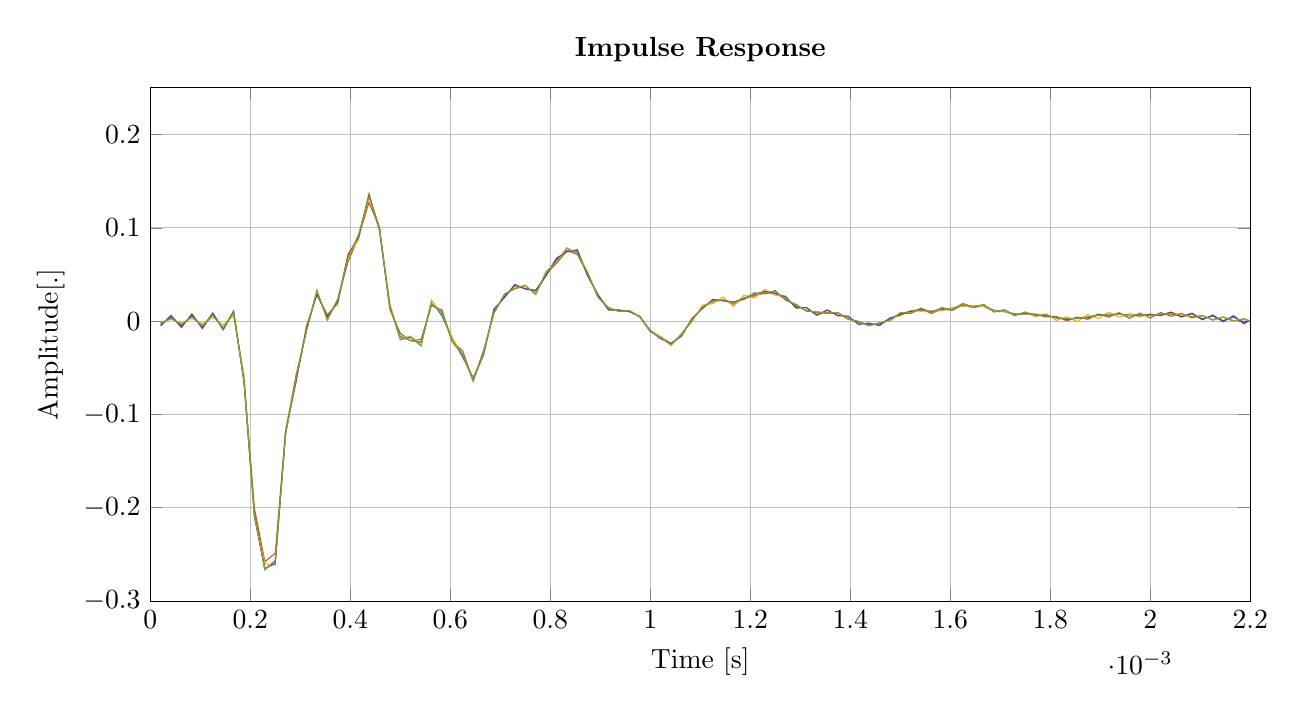
\begin{tikzpicture}

\begin{axis}[%
width=5.5in,
height=2.566in,
at={(0.758in,0.481in)},
scale only axis,
xmin=0,
xmax=0.0022,
xlabel={Time [s]},
xmajorgrids,
ymin=-0.30,
ymax=0.25,
ylabel={Amplitude[.]},
ymajorgrids,
axis background/.style={fill=white},
title style={font=\bfseries},
title={Impulse Response}
]
\addplot [color=mycolor1,solid,forget plot]
  table[row sep=crcr]{%
2.08333333333333e-05	-0.0037087927908794\\
4.16666666666667e-05	0.00421160453226942\\
6.25e-05	-0.00520379576953817\\
8.33333333333333e-05	0.00629701654848276\\
0.000104166666666667	-0.00678651279752952\\
0.000125	0.00811356819824401\\
0.000145833333333333	-0.00884124098433367\\
0.000166666666666667	0.0107472615560426\\
0.0001875	-0.0646663577808535\\
0.000208333333333333	-0.206299821990036\\
0.000229166666666667	-0.266170671528939\\
0.00025	-0.256370669612707\\
0.000270833333333333	-0.120287541326005\\
0.000291666666666667	-0.0617180208660174\\
0.0003125	-0.00922362905565283\\
0.000333333333333333	0.0308397018576189\\
0.000354166666666667	0.0035403786890247\\
0.000375	0.0212448332280645\\
0.000395833333333333	0.0705478621795121\\
0.000416666666666667	0.0895474948933934\\
0.0004375	0.13552149422923\\
0.000458333333333333	0.097299803954558\\
0.000479166666666667	0.0171466790731723\\
0.0005	-0.0197680684506663\\
0.000520833333333333	-0.0171223102171715\\
0.000541666666666667	-0.0263656309604829\\
0.0005625	0.0219768694253305\\
0.000583333333333333	0.00560475366613178\\
0.000604166666666667	-0.0182339778631218\\
0.000625	-0.0387957025837346\\
0.000645833333333333	-0.0604621915450745\\
0.000666666666666667	-0.0363795655357155\\
0.0006875	0.0130977677372803\\
0.000708333333333333	0.0251346467322033\\
0.000729166666666667	0.039105419651278\\
0.00075	0.0346523806957789\\
0.000770833333333333	0.0322481248629661\\
0.000791666666666667	0.0493725854189164\\
0.0008125	0.0660612053755624\\
0.000833333333333333	0.0751202061643853\\
0.000854166666666667	0.0750428627194294\\
0.000875	0.048916982972921\\
0.000895833333333333	0.0274042750529549\\
0.000916666666666667	0.012118310680073\\
0.0009375	0.0119101424242984\\
0.000958333333333333	0.0100853086322103\\
0.000979166666666667	0.00544456035302204\\
0.001	-0.0112918644454638\\
0.00102083333333333	-0.0172483398553776\\
0.00104166666666667	-0.0251189065330511\\
0.0010625	-0.014558012452602\\
0.00108333333333333	0.0017134948101292\\
0.00110416666666667	0.014255079903006\\
0.001125	0.0227537754361355\\
0.00114583333333333	0.021816701937651\\
0.00116666666666667	0.0206421122092443\\
0.0011875	0.0233880957023547\\
0.00120833333333333	0.0302390075091007\\
0.00122916666666667	0.0293537948171238\\
0.00125	0.0326242279536413\\
0.00127083333333333	0.0225148202302848\\
0.00129166666666667	0.0177894930311056\\
0.0013125	0.010770331824266\\
0.00133333333333333	0.00983620954713187\\
0.00135416666666667	0.00853521175516866\\
0.001375	0.00899597167105174\\
0.00139583333333333	0.00260243594654619\\
0.00141666666666667	-0.00104701561770118\\
0.0014375	-0.00371807000382697\\
0.00145833333333333	-0.00318960626194621\\
0.00147916666666667	0.00257545774845068\\
0.0015	0.00713790465040768\\
0.00152083333333333	0.0108215910141207\\
0.00154166666666667	0.0120264444758566\\
0.0015625	0.0108261870538285\\
0.00158333333333333	0.0123450686244096\\
0.00160416666666667	0.0139129670171921\\
0.001625	0.0169005010166529\\
0.00164583333333333	0.0165791257894914\\
0.00166666666666667	0.0159045477126551\\
0.0016875	0.0116907728854056\\
0.00170833333333333	0.0102974368732395\\
0.00172916666666667	0.00768755665771632\\
0.00175	0.0082004670345183\\
0.00177083333333333	0.00731505527542035\\
0.00179166666666667	0.0054086354181059\\
0.0018125	0.00446490364319473\\
0.00183333333333333	0.00151912598295708\\
0.00185416666666667	0.00374848548552877\\
0.001875	0.00361835820665017\\
0.00189583333333333	0.00680282624355538\\
0.00191666666666667	0.00648760855183481\\
0.0019375	0.00770072765347351\\
0.00195833333333333	0.00591670768911894\\
0.00197916666666667	0.00654249543276334\\
0.002	0.00696958712555653\\
0.00202083333333333	0.00639676696262537\\
0.00204166666666667	0.00930875870313683\\
0.0020625	0.00487368778960512\\
0.00208333333333333	0.00793267565500179\\
0.00210416666666667	0.00227381220914028\\
0.002125	0.00559059790855196\\
0.00214583333333333	0.000509710927088874\\
0.00216666666666667	0.00445914830547992\\
0.0021875	-0.0013119827312339\\
0.00220833333333333	0.00204620626659837\\
0.00222916666666667	-0.00226693806170011\\
0.00225	-0.000865052032163367\\
0.00227083333333333	-0.000568466635637404\\
0.00229166666666667	-0.00176072172101629\\
0.0023125	0.001051321525168\\
0.00233333333333333	-0.00235307840318451\\
0.00235416666666667	0.00142050267868398\\
0.002375	-0.00373732644882233\\
0.00239583333333333	0.00263329200115178\\
0.00241666666666667	-0.00419384885137344\\
0.0024375	0.00356243119561722\\
0.00245833333333333	-0.00341750395084726\\
0.00247916666666667	0.00231533516568704\\
0.0025	-0.002886346397735\\
0.00252083333333333	0.000637791268280785\\
0.00254166666666667	-0.00290884766679218\\
0.0025625	-0.000629280559252555\\
0.00258333333333333	-0.00286116806569122\\
0.00260416666666667	-0.00278592644964782\\
0.002625	-0.00262193859169995\\
0.00264583333333333	-0.00474810164470427\\
0.00266666666666667	-0.00275009938116807\\
0.0026875	-0.00478816826817122\\
0.00270833333333333	-0.00324811681170597\\
0.00272916666666667	-0.0040257377623872\\
0.00275	-0.00368074892796126\\
0.00277083333333333	-0.00337062684290595\\
0.00279166666666667	-0.00370307569447635\\
0.0028125	-0.00186571326957182\\
0.00283333333333333	-0.00390602380821677\\
0.00285416666666667	-4.9752550230383e-05\\
0.002875	-0.00438323194808954\\
0.00289583333333333	0.000384386269952189\\
0.00291666666666667	-0.00453307061294354\\
0.0029375	-0.000328341601327697\\
0.00295833333333333	-0.00426336185525099\\
0.00297916666666667	-0.00128138687597425\\
0.003	-0.00414308057749922\\
0.00302083333333333	-0.00248651642821263\\
0.00304166666666667	-0.00361961427656752\\
0.0030625	-0.00400763468176544\\
0.00308333333333333	-0.0023795304299123\\
0.00310416666666667	-0.00514325156697817\\
0.003125	-0.00122625577194359\\
0.00314583333333333	-0.00545188790289689\\
0.00316666666666667	-0.000609928041986866\\
0.0031875	-0.00505013848995181\\
0.00320833333333333	5.99816839252916e-05\\
0.00322916666666667	-0.00449193406111753\\
0.00325	0.000558016389499313\\
0.00327083333333333	-0.00386841737730755\\
0.00329166666666667	0.000169965391614449\\
0.0033125	-0.00319883141842068\\
0.00333333333333333	-0.000671676767081501\\
0.00335416666666667	-0.00289606776507812\\
0.003375	-0.00113994195612087\\
0.00339583333333333	-0.00325262465554565\\
0.00341666666666667	-0.00136179764715377\\
0.0034375	-0.00360873416552366\\
0.00345833333333333	-0.00164463882761736\\
0.00347916666666667	-0.00371793269729748\\
0.0035	-0.00154353439141849\\
0.00352083333333333	-0.00403549855695194\\
0.00354166666666667	-0.000984353596708564\\
0.0035625	-0.00425443771279568\\
0.00358333333333333	-0.000672628985252431\\
0.00360416666666667	-0.00374129885739169\\
0.003625	-0.000937340861272143\\
0.00364583333333333	-0.00296533591369333\\
0.00366666666666667	-0.00130448571666488\\
0.0036875	-0.00246387735925147\\
0.00370833333333333	-0.00182327238315157\\
0.00372916666666667	-0.00173617907905828\\
0.00375	-0.00284258077794951\\
0.00377083333333333	-0.000756536202756666\\
0.00379166666666667	-0.00385114062696801\\
0.0038125	-0.000291952662999003\\
0.00383333333333333	-0.00423039940178691\\
0.00385416666666667	-0.000378549414924021\\
0.003875	-0.00428312305197425\\
0.00389583333333333	-0.000406743035733924\\
0.00391666666666667	-0.00424392197549792\\
0.0039375	-0.000625284040186809\\
0.00395833333333333	-0.00365167293604246\\
0.00397916666666667	-0.001337671135446\\
0.004	-0.00271896198950253\\
0.00402083333333333	-0.0019858020567554\\
0.00404166666666667	-0.00219062801883803\\
0.0040625	-0.00220835913204532\\
0.00408333333333333	-0.00203974929682549\\
0.00410416666666667	-0.00233913427988745\\
0.004125	-0.00185099449592134\\
0.00414583333333333	-0.00236574968059208\\
0.00416666666666667	-0.00196457798952639\\
0.0041875	-0.0019046742644009\\
0.00420833333333333	-0.00250443960036927\\
0.00422916666666667	-0.00128461530764495\\
0.00425	-0.00297296735967611\\
0.00427083333333333	-0.000992836466506577\\
0.00429166666666667	-0.00314961192994209\\
0.0043125	-0.000907894618487529\\
0.00433333333333333	-0.00328775019087989\\
0.00435416666666667	-0.000812410858858454\\
0.004375	-0.00329843852206017\\
0.00439583333333333	-0.000993520893343976\\
0.00441666666666667	-0.00296787895096846\\
0.0044375	-0.00135986816935005\\
0.00445833333333333	-0.00257683158276436\\
0.00447916666666667	-0.00150120312434058\\
0.0045	-0.00246875060820952\\
0.00452083333333333	-0.00127751762473565\\
0.00454166666666667	-0.00257055972440008\\
0.0045625	-0.000850583087086702\\
0.00458333333333333	-0.00279615291783079\\
0.00460416666666667	-0.000169229703961833\\
0.004625	-0.0033208199374696\\
0.00464583333333333	0.000762775063455069\\
0.00466666666666667	-0.00404729208587363\\
0.0046875	0.00162126259324774\\
0.00470833333333333	-0.00461429328418873\\
0.00472916666666667	0.00206634843487202\\
0.00475	-0.00479804415433337\\
0.00477083333333333	0.00203716599298341\\
0.00479166666666667	-0.00461953370883597\\
0.0048125	0.00158614710765907\\
0.00483333333333333	-0.0039600168009732\\
0.00485416666666667	0.00066992915889739\\
0.004875	-0.0027700643584047\\
0.00489583333333333	-0.000614917555245659\\
0.00491666666666667	-0.00132297677247495\\
0.0049375	-0.00190838752526078\\
0.00495833333333333	-4.06116797333875e-05\\
0.00497916666666667	-0.00288565901097666\\
0.005	0.000889847654868419\\
0.00502083333333333	-0.00349274225205263\\
0.00504166666666667	0.00137995835933047\\
0.0050625	-0.00358103532986242\\
0.00508333333333333	0.00125952593606002\\
0.00510416666666667	-0.00298112408616989\\
0.005125	0.00052817856633219\\
0.00514583333333333	-0.0019103540353447\\
0.00516666666666667	-0.000471366982676235\\
0.0051875	-0.000794234842926538\\
0.00520833333333333	-0.00141585678773726\\
};
\addplot [color=mycolor2,solid,forget plot]
  table[row sep=crcr]{%
2.08333333333333e-05	-0.00255267252938673\\
4.16666666666667e-05	0.00289958707347902\\
6.25e-05	-0.00382265239043665\\
8.33333333333333e-05	0.00482200108963299\\
0.000104166666666667	-0.00515633007307537\\
0.000125	0.00667606380308441\\
0.000145833333333333	-0.00708343055179381\\
0.000166666666666667	0.0092525375696961\\
0.0001875	-0.0607390597290135\\
0.000208333333333333	-0.200401659875795\\
0.000229166666666667	-0.257768300997275\\
0.00025	-0.248800582164502\\
0.000270833333333333	-0.117646720461853\\
0.000291666666666667	-0.0578844981508881\\
0.0003125	-0.0102016454149929\\
0.000333333333333333	0.0330014197433572\\
0.000354166666666667	0.00127667958148536\\
0.000375	0.0234190373569384\\
0.000395833333333333	0.0639275956854277\\
0.000416666666666667	0.0906470163865055\\
0.0004375	0.127123824348622\\
0.000458333333333333	0.100636329904299\\
0.000479166666666667	0.0124905457764127\\
0.0005	-0.0128509224250364\\
0.000520833333333333	-0.0212238017533485\\
0.000541666666666667	-0.0195717514784339\\
0.0005625	0.0166431551373302\\
0.000583333333333333	0.0120320299572739\\
0.000604166666666667	-0.0219158802601074\\
0.000625	-0.0320151869444835\\
0.000645833333333333	-0.0633380264022395\\
0.000666666666666667	-0.0314055759804432\\
0.0006875	0.0084423319629683\\
0.000708333333333333	0.0282626599947745\\
0.000729166666666667	0.034755671823636\\
0.00075	0.0375030938504313\\
0.000770833333333333	0.0287324780339133\\
0.000791666666666667	0.0509433983273104\\
0.0008125	0.0618381605219164\\
0.000833333333333333	0.0756881939220368\\
0.000854166666666667	0.0714587648185071\\
0.000875	0.0505304570640701\\
0.000895833333333333	0.0255469926503848\\
0.000916666666666667	0.0139977515791326\\
0.0009375	0.0105701348927955\\
0.000958333333333333	0.0111681123111772\\
0.000979166666666667	0.00467517577342191\\
0.001	-0.0100498056673259\\
0.00102083333333333	-0.0168471351248233\\
0.00104166666666667	-0.0242983429721961\\
0.0010625	-0.0138911007564663\\
0.00108333333333333	0.000815862706313863\\
0.00110416666666667	0.0148029936594\\
0.001125	0.0207210667345826\\
0.00114583333333333	0.0226963031788706\\
0.00116666666666667	0.0181062087629371\\
0.0011875	0.0242935347792987\\
0.00120833333333333	0.0271226044174566\\
0.00122916666666667	0.0301879108304438\\
0.00125	0.0297329814304771\\
0.00127083333333333	0.0236557223579554\\
0.00129166666666667	0.0158766440133432\\
0.0013125	0.011696116145808\\
0.00133333333333333	0.00871715898126307\\
0.00135416666666667	0.00871221990090018\\
0.001375	0.00864655184050639\\
0.00139583333333333	0.00219401302147165\\
0.00141666666666667	-0.000480463220486303\\
0.0014375	-0.00478793011354472\\
0.00145833333333333	-0.00214213807521797\\
0.00147916666666667	0.000610919065108282\\
0.0015	0.00822355226328271\\
0.00152083333333333	0.00831464525440903\\
0.00154166666666667	0.0130253685510728\\
0.0015625	0.00825458577231076\\
0.00158333333333333	0.0131017386199352\\
0.00160416666666667	0.0115045453955671\\
0.001625	0.0173054531317267\\
0.00164583333333333	0.0146751752014143\\
0.00166666666666667	0.0160624194214595\\
0.0016875	0.0105018463460038\\
0.00170833333333333	0.0101683646808241\\
0.00172916666666667	0.0070445186245326\\
0.00175	0.00766088993981086\\
0.00177083333333333	0.00710536523175556\\
0.00179166666666667	0.00457630122370742\\
0.0018125	0.00469420240794347\\
0.00183333333333333	0.000404005788937426\\
0.00185416666666667	0.00428370428539064\\
0.001875	0.00197599863403158\\
0.00189583333333333	0.0076578440345062\\
0.00191666666666667	0.00423011592859115\\
0.0019375	0.00909761104080475\\
0.00195833333333333	0.0030678897125246\\
0.00197916666666667	0.00859528939877386\\
0.002	0.00346894854210457\\
0.00202083333333333	0.00914620649963214\\
0.00204166666666667	0.00520410877557944\\
0.0020625	0.00832413302525314\\
0.00208333333333333	0.00346908753461933\\
0.00210416666666667	0.00610387771170956\\
0.002125	0.00108867775682093\\
0.00214583333333333	0.00419930592939649\\
0.00216666666666667	0.000319892049500485\\
0.0021875	0.00180869387049779\\
0.00220833333333333	-0.00126219037085954\\
0.00222916666666667	-0.00016649986826338\\
0.00225	-0.00292140933910888\\
0.00227083333333333	5.48115721681712e-05\\
0.00229166666666667	-0.00231838798243882\\
0.0023125	6.02159680772856e-05\\
0.00233333333333333	-0.00141553936136535\\
0.00235416666666667	-0.000969725177756748\\
0.002375	-0.00155367505348034\\
0.00239583333333333	-0.00078737578525\\
0.00241666666666667	-0.00118813913866019\\
0.0024375	-0.000351639141263614\\
0.00245833333333333	-0.000202294846823073\\
0.00247916666666667	-0.00140433733178488\\
0.0025	-0.000148481375508499\\
0.00252083333333333	-0.00229105227885144\\
0.00254166666666667	-0.00113327041550525\\
0.0025625	-0.00240289119356657\\
0.00258333333333333	-0.00221020389739753\\
0.00260416666666667	-0.00327807804462282\\
0.002625	-0.00307515395717207\\
0.00264583333333333	-0.00411499501980943\\
0.00266666666666667	-0.00404707161300406\\
0.0026875	-0.00348238100217361\\
0.00270833333333333	-0.00488806311665677\\
0.00272916666666667	-0.0026354048015551\\
0.00275	-0.00512258678524018\\
0.00277083333333333	-0.00237918958058366\\
0.00279166666666667	-0.00456717537979813\\
0.0028125	-0.00158216040976036\\
0.00283333333333333	-0.00398847584896324\\
0.00285416666666667	-0.000601313268332522\\
0.002875	-0.00369552546612422\\
0.00289583333333333	-0.000887430420175447\\
0.00291666666666667	-0.0033287586160303\\
0.0029375	-0.00196666642325469\\
0.00295833333333333	-0.00291972100094473\\
0.00297916666666667	-0.00286833083131398\\
0.003	-0.00297599955911991\\
0.00302083333333333	-0.00372065054441346\\
0.00304166666666667	-0.00284107705068402\\
0.0030625	-0.00474018439203851\\
0.00308333333333333	-0.00207488352087834\\
0.00310416666666667	-0.00536932379647781\\
0.003125	-0.00131533563026484\\
0.00314583333333333	-0.00536072637441323\\
0.00316666666666667	-0.000858022679083761\\
0.0031875	-0.00494352194507911\\
0.00320833333333333	-9.29124655160845e-05\\
0.00322916666666667	-0.00458455294834229\\
0.00325	0.000653130100906661\\
0.00327083333333333	-0.00423158530604592\\
0.00329166666666667	0.000543960512810295\\
0.0033125	-0.00379406688018271\\
0.00333333333333333	-9.66816216515342e-05\\
0.00335416666666667	-0.00353027419822252\\
0.003375	-0.000570547946950482\\
0.00339583333333333	-0.00361077269310737\\
0.00341666666666667	-0.00110650316314777\\
0.0034375	-0.00343504924741948\\
0.00345833333333333	-0.00193518158467088\\
0.00347916666666667	-0.00291655885566418\\
0.0035	-0.00243334545259287\\
0.00352083333333333	-0.00262502115222047\\
0.00354166666666667	-0.00240295393708929\\
0.0035625	-0.00239818677743936\\
0.00358333333333333	-0.00241583275384139\\
0.00360416666666667	-0.00177271872007091\\
0.003625	-0.00263795048328915\\
0.00364583333333333	-0.00127580236053149\\
0.00366666666666667	-0.00260032147781131\\
0.0036875	-0.00135047828264343\\
0.00370833333333333	-0.00248490641271397\\
0.00372916666666667	-0.00135362852201022\\
0.00375	-0.00276058505758708\\
0.00377083333333333	-0.00111545031714157\\
0.00379166666666667	-0.00304804673300568\\
0.0038125	-0.00121762006398216\\
0.00383333333333333	-0.00295967887667023\\
0.00385416666666667	-0.00152799538999958\\
0.003875	-0.00293911795913497\\
0.00389583333333333	-0.00141842129814424\\
0.00391666666666667	-0.00317139837627678\\
0.0039375	-0.00120453703812563\\
0.00395833333333333	-0.00310189945322664\\
0.00397916666666667	-0.00127577630415201\\
0.004	-0.00285323822275981\\
0.00402083333333333	-0.00123759058802548\\
0.00404166666666667	-0.00295826755744021\\
0.0040625	-0.000941733037558027\\
0.00408333333333333	-0.00317740848079844\\
0.00410416666666667	-0.000853233064771672\\
0.004125	-0.003025048708344\\
0.00414583333333333	-0.000993006404728137\\
0.00416666666666667	-0.00285059650886691\\
0.0041875	-0.000974726981488831\\
0.00420833333333333	-0.00278577246306679\\
0.00422916666666667	-0.00106359834458666\\
0.00425	-0.00243185185834133\\
0.00427083333333333	-0.00161288283600495\\
0.00429166666666667	-0.00173941306975917\\
0.0043125	-0.0023614205758312\\
0.00433333333333333	-0.00107298483413706\\
0.00435416666666667	-0.00303899121775412\\
0.004375	-0.000375970115777865\\
0.00439583333333333	-0.00388549063063888\\
0.00441666666666667	0.000541297745222786\\
0.0044375	-0.00479932669104759\\
0.00445833333333333	0.00139622726997478\\
0.00447916666666667	-0.00539810064640756\\
0.0045	0.00192488295368076\\
0.00452083333333333	-0.00560504111770523\\
0.00454166666666667	0.00224701915074393\\
0.0045625	-0.00560943314661647\\
0.00458333333333333	0.0024195452607323\\
0.00460416666666667	-0.005317466524108\\
0.004625	0.00222418518526779\\
0.00464583333333333	-0.00466166053919306\\
0.00466666666666667	0.00169427281028947\\
0.0046875	-0.00386977891617415\\
0.00470833333333333	0.00106542399644791\\
0.00472916666666667	-0.00315415940463025\\
0.00475	0.000425270653698219\\
0.00477083333333333	-0.00245902414772154\\
0.00479166666666667	-0.000313192663862794\\
0.0048125	-0.00172664645538972\\
0.00483333333333333	-0.00101569750310594\\
0.00485416666666667	-0.0010706020758985\\
0.004875	-0.00152478876973867\\
0.00489583333333333	-0.00053804913087041\\
0.00491666666666667	-0.00192301123282111\\
0.0049375	-8.46962331649506e-06\\
0.00495833333333333	-0.00234650155333196\\
0.00497916666666667	0.000517616027113713\\
0.005	-0.0026874982365122\\
0.00502083333333333	0.000837710179045122\\
0.00504166666666667	-0.00281392506940281\\
0.0050625	0.000951526220070128\\
0.00508333333333333	-0.00279809276114962\\
0.00510416666666667	0.000989617566664778\\
0.005125	-0.00267417639347939\\
0.00514583333333333	0.00086092609975851\\
0.00516666666666667	-0.00228430448627185\\
0.0051875	0.000452408493989887\\
0.00520833333333333	-0.00164854160289399\\
};
\addplot [color=mycolor3,solid,forget plot]
  table[row sep=crcr]{%
2.08333333333333e-05	-0.00163321204155689\\
4.16666666666667e-05	0.00217871738448115\\
6.25e-05	-0.00223030869416506\\
8.33333333333333e-05	0.00308085388067272\\
0.000104166666666667	-0.00283418955947869\\
0.000125	0.00387776978723627\\
0.000145833333333333	-0.00396721517720515\\
0.000166666666666667	0.00565169339153807\\
0.0001875	-0.0578645073772853\\
0.000208333333333333	-0.210568816309939\\
0.000229166666666667	-0.259955188133081\\
0.00025	-0.261242392983444\\
0.000270833333333333	-0.11541144340208\\
0.000291666666666667	-0.065082383983406\\
0.0003125	-0.00457165776378929\\
0.000333333333333333	0.0281698447908548\\
0.000354166666666667	0.00746906122663251\\
0.000375	0.017980551653853\\
0.000395833333333333	0.0719876105253128\\
0.000416666666666667	0.0872051031610365\\
0.0004375	0.136972018527987\\
0.000458333333333333	0.0979061885001598\\
0.000479166666666667	0.0190373994273952\\
0.0005	-0.0187474979071836\\
0.000520833333333333	-0.0159911997270242\\
0.000541666666666667	-0.0254207659568788\\
0.0005625	0.0222939439236886\\
0.000583333333333333	0.00762495201878726\\
0.000604166666666667	-0.0181476959053041\\
0.000625	-0.0370572954894979\\
0.000645833333333333	-0.0616897321841816\\
0.000666666666666667	-0.0357751469485512\\
0.0006875	0.0110541110800959\\
0.000708333333333333	0.0266261311666174\\
0.000729166666666667	0.0370835756321231\\
0.00075	0.0372079006439419\\
0.000770833333333333	0.0299720795056686\\
0.000791666666666667	0.0519383256345237\\
0.0008125	0.0633401602353719\\
0.000833333333333333	0.0780465129838801\\
0.000854166666666667	0.072826296030486\\
0.000875	0.0525118906030222\\
0.000895833333333333	0.025547455882416\\
0.000916666666666667	0.0148804806448951\\
0.0009375	0.0103846646000134\\
0.000958333333333333	0.0115394204404138\\
0.000979166666666667	0.00482301562556526\\
0.001	-0.0109874131473168\\
0.00102083333333333	-0.0166641078639183\\
0.00104166666666667	-0.0264021861315982\\
0.0010625	-0.0129423122730922\\
0.00108333333333333	-0.00127731842486949\\
0.00110416666666667	0.0172078145589618\\
0.001125	0.0186646164744698\\
0.00114583333333333	0.0258355733901017\\
0.00116666666666667	0.0157117601980314\\
0.0011875	0.0277803562128635\\
0.00120833333333333	0.0249411956451881\\
0.00122916666666667	0.0339131100205985\\
0.00125	0.0276834810161797\\
0.00127083333333333	0.0270876373860748\\
0.00129166666666667	0.0135486398598428\\
0.0013125	0.0146281493199383\\
0.00133333333333333	0.00630120909161602\\
0.00135416666666667	0.0114262979203145\\
0.001375	0.00625151023360393\\
0.00139583333333333	0.00469691746271263\\
0.00141666666666667	-0.00320755138194242\\
0.0014375	-0.0023665451221515\\
0.00145833333333333	-0.00501549633026936\\
0.00147916666666667	0.00337042559894113\\
0.0015	0.00557224153648716\\
0.00152083333333333	0.0113999793119524\\
0.00154166666666667	0.0105608590694505\\
0.0015625	0.0112253538955211\\
0.00158333333333333	0.0109297147864292\\
0.00160416666666667	0.0141182406444556\\
0.001625	0.0158705693922061\\
0.00164583333333333	0.0165236340426216\\
0.00166666666666667	0.0155539386955293\\
0.0016875	0.0110146959222936\\
0.00170833333333333	0.0107587084546628\\
0.00172916666666667	0.006021107065009\\
0.00175	0.00962358548745266\\
0.00177083333333333	0.00461488367395265\\
0.00179166666666667	0.00786354161870322\\
0.0018125	0.00083980837975928\\
0.00183333333333333	0.00474934129641216\\
0.00185416666666667	-0.000493640480630181\\
0.001875	0.00712827695489169\\
0.00189583333333333	0.00258517202966767\\
0.00191666666666667	0.00965080478835073\\
0.0019375	0.00421535128796295\\
0.00195833333333333	0.00807287058220521\\
0.00197916666666667	0.00433552437525072\\
0.002	0.00762144067704767\\
0.00202083333333333	0.00590796681015577\\
0.00204166666666667	0.00823247822607332\\
0.0020625	0.00624889897116549\\
0.00208333333333333	0.0051706692669312\\
0.00210416666666667	0.00513911501618462\\
0.002125	0.00157578666104142\\
0.00214583333333333	0.00419562172707041\\
0.00216666666666667	-8.17894503905048e-05\\
0.0021875	0.00249146863565593\\
0.00220833333333333	-0.00225060743894737\\
0.00222916666666667	0.000911367832004493\\
0.00225	-0.0042023273732927\\
0.00227083333333333	0.00131908623295955\\
0.00229166666666667	-0.00359422398769843\\
0.0023125	0.00130602372428194\\
0.00233333333333333	-0.0025474285480275\\
0.00235416666666667	9.12508870677423e-05\\
0.002375	-0.00251258605257109\\
0.00239583333333333	3.68184456323214e-05\\
0.00241666666666667	-0.001908222379877\\
0.0024375	0.000171602768831179\\
0.00245833333333333	-0.000565657920822165\\
0.00247916666666667	-0.00132123186706604\\
0.0025	-3.69357225569728e-05\\
0.00252083333333333	-0.00278555913442368\\
0.00254166666666667	-0.000381161411822799\\
0.0025625	-0.00363098794507625\\
0.00258333333333333	-0.000623408767812987\\
0.00260416666666667	-0.00542533906568231\\
0.002625	-0.000514434727790267\\
0.00264583333333333	-0.00727794417210567\\
0.00266666666666667	-0.000521849778767368\\
0.0026875	-0.00757661607436271\\
0.00270833333333333	-0.000543882871711502\\
0.00272916666666667	-0.00744648183443503\\
0.00275	-0.000262008073977348\\
0.00277083333333333	-0.00754898213636908\\
0.00279166666666667	0.000392125328535457\\
0.0028125	-0.00659584850012438\\
0.00283333333333333	0.000562148987953842\\
0.00285416666666667	-0.00491349124801912\\
0.002875	-4.71952709105437e-05\\
0.00289583333333333	-0.00403617308167389\\
0.00291666666666667	-0.00098491246115772\\
0.0029375	-0.00360617852387868\\
0.00295833333333333	-0.00216020792434374\\
0.00297916666666667	-0.00281031658588728\\
0.003	-0.00393642768912363\\
0.00302083333333333	-0.0019740161735394\\
0.00304166666666667	-0.00545044644123764\\
0.0030625	-0.00148724838410483\\
0.00308333333333333	-0.00609761795227659\\
0.00310416666666667	-0.000911843004845307\\
0.003125	-0.00641109553135691\\
0.00314583333333333	-6.68399286926769e-05\\
0.00316666666666667	-0.00661223381392086\\
0.0031875	0.000792942062802807\\
0.00320833333333333	-0.00605194886502256\\
0.00322916666666667	0.00119081641544235\\
0.00325	-0.00510662306890529\\
0.00327083333333333	0.0012153985699642\\
0.00329166666666667	-0.00468000094954699\\
0.0033125	0.00101706104418737\\
0.00333333333333333	-0.0044992583008872\\
0.00335416666666667	0.000373907361929023\\
0.003375	-0.00393423263359508\\
0.00339583333333333	-0.000849674035833999\\
0.00341666666666667	-0.00327675308048005\\
0.0034375	-0.00196202325455657\\
0.00345833333333333	-0.00281649981315708\\
0.00347916666666667	-0.00279172529312823\\
0.0035	-0.00199265111718659\\
0.00352083333333333	-0.00384408715258885\\
0.00354166666666667	-0.000687528632112489\\
0.0035625	-0.0048382405767023\\
0.00358333333333333	0.000411062545070974\\
0.00360416666666667	-0.00517279640746107\\
0.003625	0.00102806244718597\\
0.00364583333333333	-0.00530219593314191\\
0.00366666666666667	0.00153508609358886\\
0.0036875	-0.00561251207357299\\
0.00370833333333333	0.00167486091733119\\
0.00372916666666667	-0.00539493643036716\\
0.00375	0.00095668559377168\\
0.00377083333333333	-0.00449327302460345\\
0.00379166666666667	-0.000202453154405987\\
0.0038125	-0.00358211842714922\\
0.00383333333333333	-0.00130167335324517\\
0.00385416666666667	-0.0026300982831725\\
0.003875	-0.00263555824036522\\
0.00389583333333333	-0.00114138056803914\\
0.00391666666666667	-0.00421914845301114\\
0.0039375	0.000366426789574729\\
0.00395833333333333	-0.00531590855132645\\
0.00397916666666667	0.00132682521510946\\
0.004	-0.00589441023054478\\
0.00402083333333333	0.0020330284975877\\
0.00404166666666667	-0.00643081079363684\\
0.0040625	0.00258116813465071\\
0.00408333333333333	-0.00669153743716035\\
0.00410416666666667	0.00252712937339086\\
0.004125	-0.00626501890081867\\
0.00414583333333333	0.00198573399042622\\
0.00416666666666667	-0.00564706489609503\\
0.0041875	0.00152112304451762\\
0.00420833333333333	-0.00515083718413495\\
0.00422916666666667	0.00102298995925469\\
0.00425	-0.00449765039675646\\
0.00427083333333333	0.000268338619425756\\
0.00429166666666667	-0.00371379195250488\\
0.0043125	-0.000425640222728158\\
0.00433333333333333	-0.00319524784033904\\
0.00435416666666667	-0.000821975064880745\\
0.004375	-0.00282770222093157\\
0.00439583333333333	-0.00126508575246811\\
0.00441666666666667	-0.00230471738176367\\
0.0044375	-0.00177566551043765\\
0.00445833333333333	-0.00179693413328159\\
0.00447916666666667	-0.00209730578453145\\
0.0045	-0.00146755955861572\\
0.00452083333333333	-0.00224017373487703\\
0.00454166666666667	-0.00112128092359989\\
0.0045625	-0.00241988879033352\\
0.00458333333333333	-0.000677054033918395\\
0.00460416666666667	-0.00251242284809268\\
0.004625	-0.000408875554688982\\
0.00464583333333333	-0.00238920768851963\\
0.00466666666666667	-0.00035233334164938\\
0.0046875	-0.0021916507379531\\
0.00470833333333333	-0.000353204672140455\\
0.00472916666666667	-0.00206426554660433\\
0.00475	-0.000399111146290863\\
0.00477083333333333	-0.00190898307931796\\
0.00479166666666667	-0.000620985892132324\\
0.0048125	-0.00165238099799337\\
0.00483333333333333	-0.000881278130450417\\
0.00485416666666667	-0.00142045191052985\\
0.004875	-0.00100160951886526\\
0.00489583333333333	-0.00128622165651065\\
0.00491666666666667	-0.00103775843243032\\
0.0049375	-0.00112884862974338\\
0.00495833333333333	-0.00112433334285194\\
0.00497916666666667	-0.000926118130786855\\
0.005	-0.00116589196730782\\
0.00502083333333333	-0.00085433505620867\\
0.00504166666666667	-0.00107320946693262\\
0.0050625	-0.000875743054272184\\
0.00508333333333333	-0.000966483466824754\\
0.00510416666666667	-0.000820897375894202\\
0.005125	-0.000917689548129309\\
0.00514583333333333	-0.000784404643824917\\
0.00516666666666667	-0.00076358766070243\\
0.0051875	-0.000910640434007906\\
0.00520833333333333	-0.000481400776064074\\
};
\addplot [color=mycolor4,solid,forget plot]
  table[row sep=crcr]{%
2.08333333333333e-05	-0.00516726277486403\\
4.16666666666667e-05	0.00618610543992257\\
6.25e-05	-0.00674403357522682\\
8.33333333333333e-05	0.00770721377255318\\
0.000104166666666667	-0.0079390099384032\\
0.000125	0.0086020434024014\\
0.000145833333333333	-0.00902843756603243\\
0.000166666666666667	0.0100058461757606\\
0.0001875	-0.0641955735500921\\
0.000208333333333333	-0.208700228894356\\
0.000229166666666667	-0.265220840886755\\
0.00025	-0.259647179573132\\
0.000270833333333333	-0.118446743512368\\
0.000291666666666667	-0.0645851736784997\\
0.0003125	-0.00681068819516621\\
0.000333333333333333	0.0287361417369287\\
0.000354166666666667	0.00528308056129979\\
0.000375	0.0203557265501783\\
0.000395833333333333	0.0712760448789094\\
0.000416666666666667	0.0904990248217112\\
0.0004375	0.135055068926438\\
0.000458333333333333	0.0997502441326314\\
0.000479166666666667	0.0149656960420083\\
0.0005	-0.0165087379404821\\
0.000520833333333333	-0.0206907204364962\\
0.000541666666666667	-0.0225262866903627\\
0.0005625	0.0180825474272777\\
0.000583333333333333	0.00939702452084589\\
0.000604166666666667	-0.0220080878731115\\
0.000625	-0.0359484501101515\\
0.000645833333333333	-0.0635737161406537\\
0.000666666666666667	-0.0345952872075129\\
0.0006875	0.011395100325966\\
0.000708333333333333	0.0259765767874302\\
0.000729166666666667	0.0388948268072226\\
0.00075	0.0345433960194401\\
0.000770833333333333	0.0330594608503968\\
0.000791666666666667	0.0486818198528796\\
0.0008125	0.0674756758742106\\
0.000833333333333333	0.0744150741225028\\
0.000854166666666667	0.0764475561324374\\
0.000875	0.0484555353578298\\
0.000895833333333333	0.0280952139333538\\
0.000916666666666667	0.0120915320156524\\
0.0009375	0.0116550564182299\\
0.000958333333333333	0.0106926921212952\\
0.000979166666666667	0.00437971585193512\\
0.001	-0.0101887902933229\\
0.00102083333333333	-0.0188499921570428\\
0.00104166666666667	-0.0238914746704615\\
0.0010625	-0.0161256173139097\\
0.00108333333333333	0.00275773204942341\\
0.00110416666666667	0.0133609332400136\\
0.001125	0.0231917904276933\\
0.00114583333333333	0.0219589661063437\\
0.00116666666666667	0.0200640545884449\\
0.0011875	0.0247466765973178\\
0.00120833333333333	0.0285547492678105\\
0.00122916666666667	0.0318926492272145\\
0.00125	0.0299764686613089\\
0.00127083333333333	0.0258669723089619\\
0.00129166666666667	0.0144614250473965\\
0.0013125	0.0144118803872106\\
0.00133333333333333	0.00631500520940795\\
0.00135416666666667	0.0119590422551788\\
0.001375	0.00582578414624001\\
0.00139583333333333	0.00531310542364779\\
0.00141666666666667	-0.00343872304963442\\
0.0014375	-0.00204564952450211\\
0.00145833333333333	-0.00450517778079939\\
0.00147916666666667	0.00314623347351362\\
0.0015	0.00701711951470965\\
0.00152083333333333	0.0103864197390258\\
0.00154166666666667	0.0129433271786474\\
0.0015625	0.00958576326911167\\
0.00158333333333333	0.0139841965278157\\
0.00160416666666667	0.0121875227655739\\
0.001625	0.0188998385691284\\
0.00164583333333333	0.0146984545420619\\
0.00166666666666667	0.017899680479795\\
0.0016875	0.00991070284736272\\
0.00170833333333333	0.0120138300378153\\
0.00172916666666667	0.00618896675135314\\
0.00175	0.00950797333791057\\
0.00177083333333333	0.00619846562183273\\
0.00179166666666667	0.00629933583354124\\
0.0018125	0.00372292860313401\\
0.00183333333333333	0.00204703775903457\\
0.00185416666666667	0.00329997560254824\\
0.001875	0.00389942548298164\\
0.00189583333333333	0.00657336211721742\\
0.00191666666666667	0.00665232357684192\\
0.0019375	0.0075909095931576\\
0.00195833333333333	0.00605956480100092\\
0.00197916666666667	0.00643341074030218\\
0.002	0.00717334955571132\\
0.00202083333333333	0.00619094312126556\\
0.00204166666666667	0.00966268883294692\\
0.0020625	0.00447138766764083\\
0.00208333333333333	0.00851776245037382\\
0.00210416666666667	0.00155152096694671\\
0.002125	0.00648868394668762\\
0.00214583333333333	-0.000624254648236403\\
0.00216666666666667	0.00576389327580217\\
0.0021875	-0.00289608729956137\\
0.00220833333333333	0.00381430664759555\\
0.00222916666666667	-0.00430459453439456\\
0.00225	0.00134150752329004\\
0.00227083333333333	-0.00298934954772144\\
0.00229166666666667	0.0007768827629351\\
0.0023125	-0.00158590032820341\\
0.00233333333333333	0.000330823136554005\\
0.00235416666666667	-0.00120844519950964\\
0.002375	-0.00116242832138357\\
0.00239583333333333	0.000270897000981958\\
0.00241666666666667	-0.00201802007393254\\
0.0024375	0.00171605320113375\\
0.00245833333333333	-0.00189929643819731\\
0.00247916666666667	0.00119292465952919\\
0.0025	-0.00219131249110632\\
0.00252083333333333	0.00034848939930505\\
0.00254166666666667	-0.00308860740556768\\
0.0025625	-7.85444650659138e-05\\
0.00258333333333333	-0.00384468350111693\\
0.00260416666666667	-0.001493892750237\\
0.002625	-0.00424672879397181\\
0.00264583333333333	-0.00291918864331946\\
0.00266666666666667	-0.00479474830368327\\
0.0026875	-0.002641114801147\\
0.00270833333333333	-0.00547650846681502\\
0.00272916666666667	-0.00176808208131012\\
0.00275	-0.00592170930056437\\
0.00277083333333333	-0.00117173805459234\\
0.00279166666666667	-0.00584231268464412\\
0.0028125	0.000183416280875907\\
0.00283333333333333	-0.00587588613878243\\
0.00285416666666667	0.0018311578583298\\
0.002875	-0.00616980594985171\\
0.00289583333333333	0.0020919430151921\\
0.00291666666666667	-0.006151463925198\\
0.0029375	0.00119796832713895\\
0.00295833333333333	-0.00570267165304615\\
0.00297916666666667	4.97538939356161e-05\\
0.003	-0.0053605861684554\\
0.00302083333333333	-0.00139144543259947\\
0.00304166666666667	-0.00458129470306718\\
0.0030625	-0.00320046711294441\\
0.00308333333333333	-0.00305431263079126\\
0.00310416666666667	-0.00462620972474146\\
0.003125	-0.00160809005656759\\
0.00314583333333333	-0.00518032903383794\\
0.00316666666666667	-0.000778828524857652\\
0.0031875	-0.00492703718563742\\
0.00320833333333333	-4.10939251716325e-05\\
0.00322916666666667	-0.00433900614737377\\
0.00325	0.000347078062520911\\
0.00327083333333333	-0.00349915815918508\\
0.00329166666666667	-0.000345438155645781\\
0.0033125	-0.00247367565948003\\
0.00333333333333333	-0.0016228163755218\\
0.00335416666666667	-0.00173586071389316\\
0.003375	-0.00251999805022344\\
0.00339583333333333	-0.00171285302918648\\
0.00341666666666667	-0.00302092317198616\\
0.0034375	-0.00191969840041333\\
0.00345833333333333	-0.00329477827695596\\
0.00347916666666667	-0.00222733101286352\\
0.0035	-0.00278909601039485\\
0.00352083333333333	-0.00313282923717919\\
0.00354166666666667	-0.00142955103237562\\
0.0035625	-0.00431138062946915\\
0.00358333333333333	-3.33267261560497e-05\\
0.00360416666666667	-0.0049806079600091\\
0.003625	0.000902408321895213\\
0.00364583333333333	-0.00536893329483935\\
0.00366666666666667	0.00161789846540582\\
0.0036875	-0.00579773498379327\\
0.00370833333333333	0.00182795311672953\\
0.00372916666666667	-0.00557217327052572\\
0.00375	0.00104090968872704\\
0.00377083333333333	-0.0045546501000046\\
0.00379166666666667	-0.000273437893586971\\
0.0038125	-0.00354077521085939\\
0.00383333333333333	-0.00141145409669622\\
0.00385416666666667	-0.00271206804832079\\
0.003875	-0.00247321532142388\\
0.00389583333333333	-0.00169972572390624\\
0.00391666666666667	-0.00343380518886849\\
0.0039375	-0.00103182782045088\\
0.00395833333333333	-0.00356096203020484\\
0.00397916666666667	-0.00124689158572549\\
0.004	-0.00285848083433616\\
0.00402083333333333	-0.00193851180094236\\
0.00404166666666667	-0.00200171008123463\\
0.0040625	-0.00275304267616449\\
0.00408333333333333	-0.00103788142726822\\
0.00410416666666667	-0.00387443903731943\\
0.004125	0.000250332702166949\\
0.00414583333333333	-0.00503566614560924\\
0.00416666666666667	0.00122945847968764\\
0.0041875	-0.00556311097230783\\
0.00420833333333333	0.0014705518678144\\
0.00422916666666667	-0.00551042844031363\\
0.00425	0.00127573534719517\\
0.00427083333333333	-0.00519138019590722\\
0.00429166666666667	0.000791747966865656\\
0.0043125	-0.00450084129703969\\
0.00433333333333333	-0.000179976284996915\\
0.00435416666666667	-0.00337897630774022\\
0.004375	-0.00132428816441232\\
0.00439583333333333	-0.00236086513146179\\
0.00441666666666667	-0.00212590659001618\\
0.0044375	-0.00169406418351993\\
0.00445833333333333	-0.00258120154967261\\
0.00447916666666667	-0.00124714980896368\\
0.0045	-0.0027946124294982\\
0.00452083333333333	-0.0010264231051049\\
0.00454166666666667	-0.00259422704283543\\
0.0045625	-0.00120926212080473\\
0.00458333333333333	-0.00197467115141151\\
0.00460416666666667	-0.00159779592776522\\
0.004625	-0.0013254680185666\\
0.00464583333333333	-0.00189992416851517\\
0.00466666666666667	-0.000856508408770266\\
0.0046875	-0.0020937771176436\\
0.00470833333333333	-0.000554077649769015\\
0.00472916666666667	-0.00222634800577962\\
0.00475	-0.000468283944067134\\
0.00477083333333333	-0.00214263857559105\\
0.00479166666666667	-0.000747724939442115\\
0.0048125	-0.00175014592789651\\
0.00483333333333333	-0.00125089656112911\\
0.00485416666666667	-0.00122524421554398\\
0.004875	-0.00171841491726784\\
0.00489583333333333	-0.000745651416354775\\
0.00491666666666667	-0.00209130880535271\\
0.0049375	-0.000296459854376949\\
0.00495833333333333	-0.00242018361148765\\
0.00497916666666667	9.12195276498172e-05\\
0.005	-0.00257540275405454\\
0.00502083333333333	0.000207506743761061\\
0.00504166666666667	-0.00243009552772572\\
0.0050625	7.70973327593161e-05\\
0.00508333333333333	-0.00213121004529441\\
0.00510416666666667	-7.55027093919094e-05\\
0.005125	-0.00183247624499863\\
0.00514583333333333	-0.000241500753831187\\
0.00516666666666667	-0.00146441363258871\\
0.0051875	-0.00050067414854697\\
0.00520833333333333	-0.0010689724886638\\
};
\addplot [color=mycolor5,solid,forget plot]
  table[row sep=crcr]{%
2.08333333333333e-05	-0.00183694080367487\\
4.16666666666667e-05	0.00269775576535856\\
6.25e-05	-0.00330864487443258\\
8.33333333333333e-05	0.00446922873033606\\
0.000104166666666667	-0.00511216151187469\\
0.000125	0.00628161008825259\\
0.000145833333333333	-0.00739773060073078\\
0.000166666666666667	0.00918365663237817\\
0.0001875	-0.0640643771063412\\
0.000208333333333333	-0.207629084903728\\
0.000229166666666667	-0.266512571802307\\
0.00025	-0.256975404662541\\
0.000270833333333333	-0.121150763678526\\
0.000291666666666667	-0.0611548539632256\\
0.0003125	-0.0104129176519418\\
0.000333333333333333	0.0323067772127556\\
0.000354166666666667	0.00164090751066485\\
0.000375	0.0236255560777956\\
0.000395833333333333	0.06830166976313\\
0.000416666666666667	0.0929087418121704\\
0.0004375	0.13301902945068\\
0.000458333333333333	0.100936103236603\\
0.000479166666666667	0.0140285669386969\\
0.0005	-0.0161700462857896\\
0.000520833333333333	-0.0208468721314891\\
0.000541666666666667	-0.0226220402462128\\
0.0005625	0.0180740728030884\\
0.000583333333333333	0.00931391260236883\\
0.000604166666666667	-0.0223811360937609\\
0.000625	-0.0351734754640771\\
0.000645833333333333	-0.0647259979556037\\
0.000666666666666667	-0.0325867644033155\\
0.0006875	0.00898058450624136\\
0.000708333333333333	0.0291265867299432\\
0.000729166666666667	0.0352941328824218\\
0.00075	0.0385603213063728\\
0.000770833333333333	0.028737201659164\\
0.000791666666666667	0.0530826006757693\\
0.0008125	0.0629821946361526\\
0.000833333333333333	0.0785023152976803\\
0.000854166666666667	0.0724206512475182\\
0.000875	0.0516411907781996\\
0.000895833333333333	0.0252766828649511\\
0.000916666666666667	0.0140481289383357\\
0.0009375	0.0103486623306802\\
0.000958333333333333	0.011288134477749\\
0.000979166666666667	0.00452179861807155\\
0.001	-0.0108066056383279\\
0.00102083333333333	-0.0175992589402696\\
0.00104166666666667	-0.0253128018813454\\
0.0010625	-0.0143504620645333\\
0.00108333333333333	0.00103019786277436\\
0.00110416666666667	0.0149760846537094\\
0.001125	0.021772751579079\\
0.00114583333333333	0.0229129142405795\\
0.00116666666666667	0.0195261483333946\\
0.0011875	0.0247111551394756\\
0.00120833333333333	0.029165953038416\\
0.00122916666666667	0.0306951510029648\\
0.00125	0.0317127991700103\\
0.00127083333333333	0.0235587890851777\\
0.00129166666666667	0.0171755554809782\\
0.0013125	0.0113317115131608\\
0.00133333333333333	0.00966950258690897\\
0.00135416666666667	0.0084848262426318\\
0.001375	0.00936025782752537\\
0.00139583333333333	0.0018605258760557\\
0.00141666666666667	-0.00011667583265064\\
0.0014375	-0.00508943015759043\\
0.00145833333333333	-0.0016939190207471\\
0.00147916666666667	0.000756684386819692\\
0.0015	0.00906821913097466\\
0.00152083333333333	0.00875811174534595\\
0.00154166666666667	0.0142045150007034\\
0.0015625	0.00872550078162829\\
0.00158333333333333	0.014561042442384\\
0.00160416666666667	0.0119283605131355\\
0.001625	0.0189699720965624\\
0.00164583333333333	0.0147986619876687\\
0.00166666666666667	0.0177291717017055\\
0.0016875	0.0101130470467348\\
0.00170833333333333	0.011891104230609\\
0.00172916666666667	0.00626330567477195\\
0.00175	0.00964315574422997\\
0.00177083333333333	0.00597610694387428\\
0.00179166666666667	0.00676900938218093\\
0.0018125	0.00316921417751703\\
0.00183333333333333	0.00276978914393364\\
0.00185416666666667	0.00255747544219039\\
0.001875	0.00465507490137383\\
0.00189583333333333	0.00593605006847284\\
0.00191666666666667	0.00710918977577941\\
0.0019375	0.00743396864256613\\
0.00195833333333333	0.00582624150445395\\
0.00197916666666667	0.0071523110382564\\
0.002	0.00590320742513466\\
0.00202083333333333	0.00808548307245867\\
0.00204166666666667	0.00714310325999776\\
0.0020625	0.00765039599172813\\
0.00208333333333333	0.00474811998548259\\
0.00210416666666667	0.0059146576224379\\
0.002125	0.00170546171762879\\
0.00214583333333333	0.00459490612183377\\
0.00216666666666667	0.000384874437928168\\
0.0021875	0.00263820817769318\\
0.00220833333333333	-0.00160695364388704\\
0.00222916666666667	0.000938425698385665\\
0.00225	-0.00350150608652209\\
0.00227083333333333	0.00138650915064656\\
0.00229166666666667	-0.00296735858372556\\
0.0023125	0.00147981611955108\\
0.00233333333333333	-0.00197569061842833\\
0.00235416666666667	0.000332672141494042\\
0.002375	-0.00193276417796099\\
0.00239583333333333	0.000332534578102534\\
0.00241666666666667	-0.00142123405521269\\
0.0024375	0.000595464433092438\\
0.00245833333333333	-0.00033104378088869\\
0.00247916666666667	-0.000628383127052637\\
0.0025	-0.000169100125387944\\
0.00252083333333333	-0.00164286774990944\\
0.00254166666666667	-0.00113799929739703\\
0.0025625	-0.00177840315394551\\
0.00258333333333333	-0.00237794743376311\\
0.00260416666666667	-0.00260136378649268\\
0.002625	-0.0034614841347566\\
0.00264583333333333	-0.00334881363572188\\
0.00266666666666667	-0.00462956933162578\\
0.0026875	-0.00256706460360964\\
0.00270833333333333	-0.00567233074670817\\
0.00272916666666667	-0.00153868789833283\\
0.00275	-0.00607358828586136\\
0.00277083333333333	-0.00118775776784012\\
0.00279166666666667	-0.00554868783532898\\
0.0028125	-0.000431878221958489\\
0.00283333333333333	-0.00486521252255728\\
0.00285416666666667	0.000426252118386822\\
0.002875	-0.00437077474685128\\
0.00289583333333333	-3.83248125346931e-05\\
0.00291666666666667	-0.00372540750621784\\
0.0029375	-0.00137072864831652\\
0.00295833333333333	-0.00302943173806034\\
0.00297916666666667	-0.00254314874047966\\
0.003	-0.00292382710021425\\
0.00302083333333333	-0.00353654515648264\\
0.00304166666666667	-0.00281368240423307\\
0.0030625	-0.004499148008335\\
0.00308333333333333	-0.00225798395795248\\
0.00310416666666667	-0.00488821397948152\\
0.003125	-0.00187549848927019\\
0.00314583333333333	-0.00444266842303002\\
0.00316666666666667	-0.00194977818768166\\
0.0031875	-0.00343438772121835\\
0.00320833333333333	-0.00177950707108735\\
0.00322916666666667	-0.00249719170032265\\
0.00325	-0.00153676165081829\\
0.00327083333333333	-0.00173496062595026\\
0.00329166666666667	-0.00196146225602646\\
0.0033125	-0.00111887307647677\\
0.00333333333333333	-0.00270592071654781\\
0.00335416666666667	-0.000951400411222539\\
0.003375	-0.00303583979618812\\
0.00339583333333333	-0.00143553914342979\\
0.00341666666666667	-0.00315235230276506\\
0.0034375	-0.00185287085480954\\
0.00345833333333333	-0.00340088496393738\\
0.00347916666666667	-0.00195651949418887\\
0.0035	-0.00331299548667301\\
0.00352083333333333	-0.00225045388032761\\
0.00354166666666667	-0.00274174065486804\\
0.0035625	-0.00253272575758083\\
0.00358333333333333	-0.0022950968923779\\
0.00360416666666667	-0.00226956657999736\\
0.003625	-0.00220900640785088\\
0.00364583333333333	-0.00198688824758307\\
0.00366666666666667	-0.00196129552536715\\
0.0036875	-0.00222668382155181\\
0.00370833333333333	-0.00163803328922128\\
0.00372916666666667	-0.00242135810248223\\
0.00375	-0.00169878080532646\\
0.00377083333333333	-0.00240271207890884\\
0.00379166666666667	-0.00178482766872638\\
0.0038125	-0.00276262318079547\\
0.00383333333333333	-0.00144752632322627\\
0.00385416666666667	-0.00338887691558329\\
0.003875	-0.0011235878649765\\
0.00389583333333333	-0.00360276128511714\\
0.00391666666666667	-0.0010898412082731\\
0.0039375	-0.00364761398150759\\
0.00395833333333333	-0.000816341793401194\\
0.00397916666666667	-0.00391914968305896\\
0.004	-0.000393797533269311\\
0.00402083333333333	-0.00402772214961534\\
0.00404166666666667	-0.000403815798285107\\
0.0040625	-0.00376420356641242\\
0.00408333333333333	-0.000678945405755922\\
0.00410416666666667	-0.00356193732440603\\
0.004125	-0.000724848726152835\\
0.00414583333333333	-0.00345082754139939\\
0.00416666666666667	-0.000903658924013599\\
0.0041875	-0.00300573184010322\\
0.00420833333333333	-0.00142019286324911\\
0.00422916666666667	-0.00242680786667316\\
0.00425	-0.00187867537819102\\
0.00427083333333333	-0.00207818949878901\\
0.00429166666666667	-0.00216713107510767\\
0.0043125	-0.00177009673317393\\
0.00433333333333333	-0.00260489792584533\\
0.00435416666666667	-0.00128259330924896\\
0.004375	-0.00305767497625344\\
0.00439583333333333	-0.00096352279224579\\
0.00441666666666667	-0.00319292473863172\\
0.0044375	-0.000907062555897271\\
0.00445833333333333	-0.00313354326156351\\
0.00447916666666667	-0.000880627915769135\\
0.0045	-0.00302958482048134\\
0.00452083333333333	-0.000882944723935813\\
0.00454166666666667	-0.00269240462403318\\
0.0045625	-0.00113855775118239\\
0.00458333333333333	-0.00203855379942678\\
0.00460416666666667	-0.00153500239738074\\
0.004625	-0.00137441034830759\\
0.00464583333333333	-0.00186988625816161\\
0.00466666666666667	-0.00084471616135345\\
0.0046875	-0.00216604017222241\\
0.00470833333333333	-0.000408502565127081\\
0.00472916666666667	-0.00246621265657476\\
0.00475	-0.000128850411515083\\
0.00477083333333333	-0.00259165537714265\\
0.00479166666666667	-0.000204592953846044\\
0.0048125	-0.00240350317728393\\
0.00483333333333333	-0.000525550391408901\\
0.00485416666666667	-0.00203460498841687\\
0.004875	-0.000856329521520775\\
0.00489583333333333	-0.00166039765281729\\
0.00491666666666667	-0.00113648533244863\\
0.0049375	-0.00129593544844764\\
0.00495833333333333	-0.00137336466044101\\
0.00497916666666667	-0.00101824006274034\\
0.005	-0.00138372492376765\\
0.00502083333333333	-0.00108269303633796\\
0.00504166666666667	-0.00101661529037089\\
0.0050625	-0.00148448313002126\\
0.00508333333333333	-0.00040693927282269\\
0.00510416666666667	-0.00197448809399342\\
0.005125	0.000248107014438327\\
0.00514583333333333	-0.00248830449433159\\
0.00516666666666667	0.000929192612529347\\
0.0051875	-0.00301326617479279\\
0.00520833333333333	0.00150614480417336\\
};
\end{axis}
\end{tikzpicture}%
%	\caption{Frequency Response plot of the cancellation path}
%	\label{CancellationPathImpulseResponse}
%\end{figure}

%Converting the impulse response from magnitude to dB, gives the time decay which reveals the SNR  of the system, see \autoref{TimeDecayPlotHeadphone}, and from the read off SNR is found to be $\sim$ 30 dB SNR. \todoOliver{agian - does this make sense?}

% \begin{figure}[H]
% 	\centering
% 	\tikzsetnextfilename{TimeDecayHP}
% 	% This file was created by matlab2tikz.
%
%The latest updates can be retrieved from
%  http://www.mathworks.com/matlabcentral/fileexchange/22022-matlab2tikz-matlab2tikz
%where you can also make suggestions and rate matlab2tikz.
%
\definecolor{mycolor1}{rgb}{0.00000,0.44700,0.74100}%
\definecolor{mycolor2}{rgb}{0.85000,0.32500,0.09800}%
\definecolor{mycolor3}{rgb}{0.92900,0.69400,0.12500}%
\definecolor{mycolor4}{rgb}{0.49400,0.18400,0.55600}%
\definecolor{mycolor5}{rgb}{0.46600,0.67400,0.18800}%
%
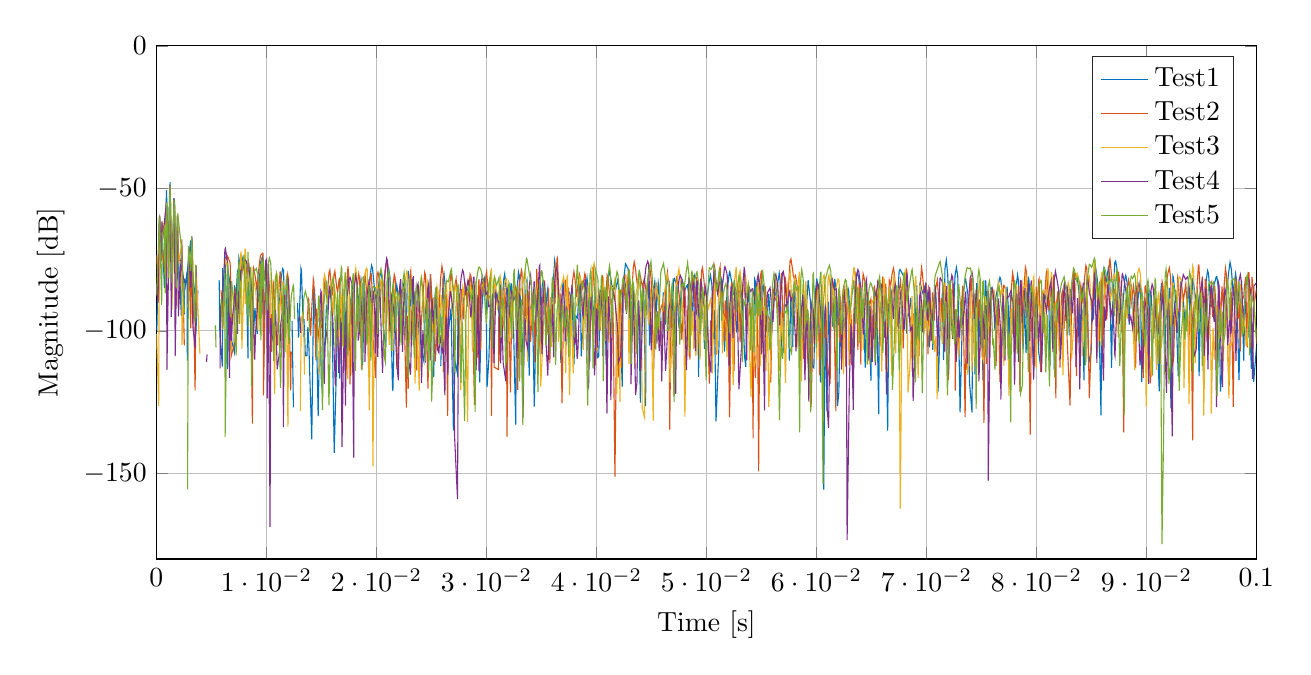
\begin{tikzpicture}

\begin{axis}[%
width=5.5in,
height=2.566in,
at={(0.758in,0.481in)},
scale only axis,
unbounded coords=jump,
xmin=0,
xmax=0.1,
xlabel={Time [s]},
xmajorgrids,
ymin=-180,
ymax=0,
ylabel={Magnitude [dB]},
ymajorgrids,
axis background/.style={fill=white},
legend style={legend cell align=left,align=left,draw=white!15!black}
]
\addplot [color=mycolor1,solid]
  table[row sep=crcr]{%
2.08333333333333e-05	-97.3654514577734\\
4.16666666666667e-05	-99.6356898741396\\
0.000270833333333333	-60.814904278184\\
0.000291666666666667	-59.578654578049\\
0.000479166666666667	-73.0072396477299\\
0.0005	-61.7445517701191\\
0.000729166666666667	-84.8917479891315\\
0.000729166666666667	-84.8917479891315\\
0.000916666666666667	-50.6543138087346\\
0.00110416666666667	-74.5511161675783\\
0.0011875	-53.4175371836811\\
0.00125	-47.8461585131505\\
0.00141666666666667	-87.8644365318066\\
0.00141666666666667	-87.8644365318066\\
0.00160416666666667	-53.4075415202207\\
0.00164583333333333	-54.8342897469004\\
0.00183333333333333	-86.7280617123974\\
0.00191666666666667	-59.7879315057733\\
0.00195833333333333	-70.0554477249167\\
0.00227083333333333	-94.7701369815506\\
0.00229166666666667	-71.5857728207153\\
0.00254166666666667	-94.2012786287276\\
0.0025625	-81.6414451608046\\
0.00258333333333333	-85.7454080529579\\
0.00279166666666667	-79.1568446279278\\
0.0028125	-110.428134543523\\
0.00283333333333333	-78.1026920680389\\
0.003125	-68.2689894744826\\
0.00322916666666667	-88.1072460587269\\
0.00325	-78.5722915769618\\
0.00325	-78.5722915769618\\
0.0035625	-89.168510925881\\
0.00358333333333333	-101.065868925642\\
0.00377083333333333	-85.7675629656821\\
0.00377083333333333	-85.7675629656821\\
0.00395833333333333	nan\\
0.00395833333333333	nan\\
0.0041875	nan\\
0.0041875	nan\\
0.00441666666666667	nan\\
0.00441666666666667	nan\\
0.00464583333333333	nan\\
0.00464583333333333	nan\\
0.004875	nan\\
0.004875	nan\\
0.00510416666666667	nan\\
0.00510416666666667	nan\\
0.00533333333333333	nan\\
0.00533333333333333	nan\\
0.00570833333333333	-82.2055644793463\\
0.00577083333333333	-101.502733975155\\
0.006	-112.493542587173\\
0.00602083333333333	-78.017326822528\\
0.00604166666666667	-94.9050154414607\\
0.00622916666666667	-73.8012878184391\\
0.00627083333333333	-74.4233191140965\\
0.00647916666666667	-113.39569384444\\
0.00647916666666667	-113.39569384444\\
0.0065	-78.4651178508884\\
0.00670833333333333	-83.8156680569606\\
0.00685416666666667	-103.610181328667\\
0.00708333333333333	-107.354345824412\\
0.00710416666666667	-83.9950386306081\\
0.00722916666666667	-89.451827729728\\
0.007375	-78.5749002317498\\
0.00739583333333333	-86.2814285915024\\
0.0075	-74.3713566050045\\
0.00775	-78.9126595543432\\
0.0078125	-74.6356450870641\\
0.00789583333333333	-75.9956355777711\\
0.00808333333333333	-80.1250088556294\\
0.00814583333333333	-77.5116119927019\\
0.00833333333333333	-109.605644736316\\
0.00833333333333333	-109.605644736316\\
0.00835416666666667	-82.6821895331865\\
0.0085625	-96.8636011674553\\
0.00860416666666667	-106.94646411898\\
0.008875	-97.8717452430268\\
0.00895833333333333	-92.0588984155785\\
0.00916666666666667	-101.00104972321\\
0.00922916666666667	-80.8612784321349\\
0.00925	-89.6976549651118\\
0.00945833333333333	-76.1425443862059\\
0.009625	-74.2152414676393\\
0.0096875	-94.211219965354\\
0.00970833333333333	-74.5500611380228\\
0.00972916666666667	-105.426118271792\\
0.00995833333333333	-76.4197187271558\\
0.0101666666666667	-86.6858924079583\\
0.0101666666666667	-86.6858924079583\\
0.01025	-100.689012758453\\
0.0103958333333333	nan\\
0.0103958333333333	nan\\
0.010625	nan\\
0.010625	nan\\
0.0110625	-100.566580203119\\
0.0110625	-100.566580203119\\
0.0111041666666667	-95.6052944443533\\
0.0113125	-82.2732024470356\\
0.0113125	-82.2732024470356\\
0.0114791666666667	-78.1899302026511\\
0.0115625	-78.8310302393297\\
0.0117083333333333	-102.326342255058\\
0.0118333333333333	-86.1679005868\\
0.012	-102.329144034274\\
0.0120208333333333	nan\\
0.0120208333333333	nan\\
0.0123333333333333	-96.5165819718347\\
0.0124583333333333	-126.848512352262\\
0.0124791666666667	nan\\
0.0124791666666667	nan\\
0.0128333333333333	-90.1833243953264\\
0.0129166666666667	-102.311968395831\\
0.0129375	-101.715820008022\\
0.0131458333333333	-78.0790880374129\\
0.0131875	-78.9235850066278\\
0.013375	-102.153944213765\\
0.0134166666666667	-95.8359350503214\\
0.0135416666666667	-108.716644761505\\
0.0136875	-108.673114930698\\
0.0137708333333333	-98.5900875197679\\
0.0138541666666667	-104.033032737022\\
0.0138541666666667	-104.033032737022\\
0.014125	-138.060790695177\\
0.0142916666666667	-86.7210793824493\\
0.014375	-85.6525808995322\\
0.0145416666666667	-98.7929861379935\\
0.0145416666666667	-98.7929861379935\\
0.0147083333333333	-129.884543958335\\
0.014875	-92.6780424466257\\
0.015	-118.472774780152\\
0.0151041666666667	-120.5546993221\\
0.0151875	-102.620677473445\\
0.0152291666666667	-114.566199749248\\
0.0154583333333333	-91.4155255048211\\
0.0155833333333333	-92.7058447289477\\
0.0157083333333333	-87.0487390451611\\
0.0157916666666667	-85.2716385857263\\
0.0159166666666667	-88.081158142176\\
0.0159583333333333	-91.3712536418906\\
0.0161666666666667	-142.760530197766\\
0.0161666666666667	-142.760530197766\\
0.0163958333333333	-108.711868314922\\
0.0163958333333333	-108.711868314922\\
0.0164791666666667	-96.3614626610975\\
0.0166666666666667	-116.701902253421\\
0.01675	-95.4508702293966\\
0.0168958333333333	-99.5128289815832\\
0.0170625	-85.1662970237552\\
0.0172083333333333	-106.183033193754\\
0.0172916666666667	-85.2325550708774\\
0.0174166666666667	-80.8143517060504\\
0.0175416666666667	-86.0877930964014\\
0.0176875	-93.862856703655\\
0.0177708333333333	-85.8190356070418\\
0.0177708333333333	-85.8190356070418\\
0.0179791666666667	-81.670759320313\\
0.0181041666666667	-80.4643894408839\\
0.0182291666666667	-83.3156279850759\\
0.0182291666666667	-83.3156279850759\\
0.0183958333333333	-91.2742546177765\\
0.0184791666666667	-86.6631687728661\\
0.0186041666666667	-81.7127216764156\\
0.0186875	-83.4204982730311\\
0.01875	-111.969215487373\\
0.0189166666666667	-85.892736077567\\
0.0190208333333333	-97.4132259872516\\
0.0192291666666667	-87.714755134631\\
0.0193958333333333	-81.8553892590245\\
0.0193958333333333	-81.8553892590245\\
0.0195625	-76.974741271216\\
0.0196458333333333	-77.9409930538186\\
0.0198541666666667	-86.2748889018603\\
0.0198541666666667	-86.2748889018603\\
0.0199791666666667	-89.435855269906\\
0.0201041666666667	-87.1628390181187\\
0.0203125	-80.418774675924\\
0.0203958333333333	-79.204742825199\\
0.0205208333333333	-81.9102618799\\
0.0205625	-84.0265400661068\\
0.020625	-98.7126970323639\\
0.0208541666666667	-105.807396749602\\
0.021	-81.0145446653181\\
0.021	-81.0145446653181\\
0.021125	-78.2316882226389\\
0.02125	-81.6211509366863\\
0.0214583333333333	-119.343901340996\\
0.0215	-121.088963904891\\
0.0216875	-88.8949242463845\\
0.0216875	-88.8949242463845\\
0.0218541666666667	-83.9564289084137\\
0.0219375	-86.2692209936706\\
0.0220625	-105.379826218147\\
0.0221666666666667	-88.1564969280095\\
0.022375	-84.9151062048753\\
0.022375	-84.9151062048753\\
0.0225416666666667	-82.8630628146872\\
0.0227083333333333	-103.289823001546\\
0.0228125	-81.7897504778737\\
0.0228958333333333	-78.9520316878626\\
0.0230625	-87.3831390312526\\
0.0230625	-87.3831390312526\\
0.0231875	-105.100375456256\\
0.0233958333333333	-86.3695169693059\\
0.0235208333333333	-90.2027439746249\\
0.0235625	-94.9120371294943\\
0.02375	-105.620613212385\\
0.0237916666666667	-99.1388159295498\\
0.0239166666666667	-94.4319695060876\\
0.024	-96.7711506637548\\
0.024125	-107.802950670262\\
0.0243125	-110.640653287546\\
0.0244375	-93.9558830569452\\
0.0245625	-89.3188497217328\\
0.0246875	-103.921423091778\\
0.0246875	-103.921423091778\\
0.0249166666666667	-80.0807724663776\\
0.0249166666666667	-80.0807724663776\\
0.025125	-93.5091789519635\\
0.0252083333333333	-116.216412072787\\
0.025375	-86.622216214789\\
0.0254166666666667	-85.8701117009112\\
0.0255416666666667	-95.871903172994\\
0.0256041666666667	nan\\
0.0256041666666667	nan\\
0.0258541666666667	-112.364213701279\\
0.0260625	-81.2765979101625\\
0.0261458333333333	-79.9200594559355\\
0.0262708333333333	-84.6142120956751\\
0.0263125	-89.2800656989808\\
0.0264583333333333	-101.219793681268\\
0.0265833333333333	-99.0733387969677\\
0.02675	-92.8495042827364\\
0.0267916666666667	-92.2836832094264\\
0.027	-134.912085945604\\
0.027	-134.912085945604\\
0.0271458333333333	-110.528385062798\\
0.0273541666666667	-114.690650941871\\
0.0274375	-91.7589881279247\\
0.0275208333333333	-86.9515922146054\\
0.0276458333333333	-94.3567276827174\\
0.02775	-96.9239359984626\\
0.0279166666666667	-88.7084102336558\\
0.0279166666666667	-88.7084102336558\\
0.028125	-86.6969574709975\\
0.0281666666666667	-86.1593458344125\\
0.028375	-84.993841214734\\
0.028375	-84.993841214734\\
0.0285833333333333	-81.9280517153117\\
0.028625	-81.7085294284161\\
0.0288333333333333	-87.6768557056198\\
0.0288333333333333	-87.6768557056198\\
0.0290208333333333	-116.330382890985\\
0.0290833333333333	-95.291544737932\\
0.0292083333333333	-89.6827446798716\\
0.0292916666666667	-92.2562894798893\\
0.0293958333333333	-118.014273187704\\
0.0295208333333333	-97.1281714592048\\
0.0297291666666667	-83.2800590308107\\
0.0298541666666667	-81.2697052701579\\
0.0299791666666667	-87.723767295186\\
0.0299791666666667	-87.723767295186\\
0.0300625	-119.701329703909\\
0.0302291666666667	-109.79941293351\\
0.0303958333333333	-87.6474374957539\\
0.0305208333333333	-105.706910883626\\
0.0306666666666667	-85.3226050779773\\
0.0306666666666667	-85.3226050779773\\
0.030875	-90.0117356491173\\
0.0310416666666667	-87.1974314062344\\
0.031125	-92.1172464384995\\
0.0311666666666667	-107.501014514038\\
0.0313125	-83.488535775357\\
0.0314375	-92.1316961669162\\
0.0315833333333333	-81.7465551348917\\
0.0316666666666667	-80.0104132957617\\
0.0318333333333333	-86.2193616132135\\
0.0318333333333333	-86.2193616132135\\
0.0319583333333333	-92.2365280869073\\
0.0320833333333333	-88.5075100274042\\
0.03225	-83.4795325220185\\
0.0322916666666667	-83.6273091108804\\
0.0324791666666667	-100.418330684829\\
0.0326666666666667	-132.865017262885\\
0.03275	-87.4041644641227\\
0.03275	-87.4041644641227\\
0.0329166666666667	-79.3406016773817\\
0.033	-80.8116100047705\\
0.0332083333333333	-98.5702940967494\\
0.033375	-113.214231824203\\
0.0334375	-97.5491821096369\\
0.0334375	-97.5491821096369\\
0.0336458333333333	-82.6809907150878\\
0.0336875	-82.0766045717452\\
0.0338958333333333	-115.671106785299\\
0.0338958333333333	-115.671106785299\\
0.0339583333333333	-92.221815958537\\
0.0341875	-90.5690854393486\\
0.0343541666666667	-126.578439481165\\
0.0343541666666667	-126.578439481165\\
0.0345833333333333	-82.9437921858114\\
0.034625	-82.4708807617349\\
0.0348333333333333	-91.840850994255\\
0.0348958333333333	-108.170898100735\\
0.0350625	-84.6464643152086\\
0.0351458333333333	-82.6760683714658\\
0.0352708333333333	-85.1977386776634\\
0.0354166666666667	-97.5208445733808\\
0.0355	-87.3003383773203\\
0.0355833333333333	-85.2102305375097\\
0.03575	-96.9132658166172\\
0.0358125	-101.121585204553\\
0.0358541666666667	-96.0085780352399\\
0.036	-87.3788569033722\\
0.0362083333333333	-75.2876201932183\\
0.0362083333333333	-75.2876201932183\\
0.0364166666666667	-80.61206048422\\
0.0364583333333333	-82.620798510436\\
0.0366666666666667	-92.4881756119585\\
0.0367708333333333	-111.172523950152\\
0.0368958333333333	-85.246340268862\\
0.0369791666666667	-83.0722613661433\\
0.0371041666666667	-86.9081288928276\\
0.03725	-105.353217184159\\
0.0373333333333333	-89.8074238206242\\
0.037375	-87.7602190931035\\
0.0375	-86.2659379835488\\
0.0375833333333333	-86.7818620625847\\
0.0377916666666667	-91.0866642641992\\
0.0378333333333333	-92.6670172688218\\
0.0379583333333333	-111.773220122141\\
0.0380625	-101.254603879568\\
0.0381458333333333	-94.7846573601692\\
0.0382916666666667	-95.5419828907794\\
0.0384583333333333	-82.1492276342732\\
0.0385416666666667	-85.3472916157128\\
0.038625	-108.943755408813\\
0.0388958333333333	-89.5661550173275\\
0.0389791666666667	-86.8513222021502\\
0.0389791666666667	-86.8513222021502\\
0.0391458333333333	-81.3953603690972\\
0.0392291666666667	-84.500728386007\\
0.0393958333333333	-110.791145752852\\
0.0394375	-99.8958432932655\\
0.0396041666666667	-86.1689235469614\\
0.03975	-98.061052723762\\
0.039875	-84.8475910295514\\
0.0399166666666667	-85.5868365517226\\
0.0400833333333333	-109.410671500635\\
0.0402083333333333	-109.026753138586\\
0.0403333333333333	-94.1316698000096\\
0.040375	-92.4216373800094\\
0.0405	-90.5211593536829\\
0.0405833333333333	-90.8645130897045\\
0.0407916666666667	-93.1699422207915\\
0.0408958333333333	-111.751967631637\\
0.0410208333333333	-83.6387144582332\\
0.0410625	-81.2387111944224\\
0.0411875	-79.1227443854394\\
0.0412708333333333	-80.7572606227423\\
0.0414375	-84.5493182579109\\
0.0415625	-84.3045348407861\\
0.0417291666666667	-85.7780307887451\\
0.0417291666666667	-85.7780307887451\\
0.0419375	-82.1275268547366\\
0.0419791666666667	-82.4916412269324\\
0.0421041666666667	-92.9676066314922\\
0.0423541666666667	-119.494320015121\\
0.0424375	-83.6084974664229\\
0.0424375	-83.6084974664229\\
0.0426458333333333	-76.4134210299055\\
0.0426875	-76.6643600449265\\
0.0428958333333333	-78.3589011029572\\
0.0428958333333333	-78.3589011029572\\
0.0431041666666667	-103.499584996351\\
0.0432083333333333	-89.7395275340005\\
0.0433125	-101.613145038532\\
0.0433541666666667	-92.5692976193762\\
0.0434791666666667	-86.8306736754519\\
0.0436666666666667	-105.843282681938\\
0.0437916666666667	-90.3006720010803\\
0.0438333333333333	-90.3293002433172\\
0.044	-125.184127317244\\
0.0440625	-94.1655734206784\\
0.0442708333333333	-87.1648113729193\\
0.0443125	-86.7734017257581\\
0.0444791666666667	-126.287753540631\\
0.0445	-94.8571449879957\\
0.0446666666666667	-81.728282144249\\
0.04475	-84.8768061905862\\
0.0448333333333333	-105.149505400828\\
0.0451041666666667	-88.9804309445314\\
0.0451875	-86.084160207826\\
0.0453125	-82.7711290891903\\
0.0453958333333333	-86.4665576184842\\
0.0454375	-93.3377767142581\\
0.045625	-83.1441669007684\\
0.0456666666666667	-84.3126173071572\\
0.0458125	-98.9119623546122\\
0.0459375	-100.342500671474\\
0.0460833333333333	-86.506376435475\\
0.0462708333333333	-97.7416389153287\\
0.0463541666666667	-84.900099340878\\
0.0463541666666667	-84.900099340878\\
0.0464791666666667	-81.9579923084919\\
0.0466041666666667	-82.5340531756306\\
0.0468125	-98.7955839276076\\
0.0468125	-98.7955839276076\\
0.0470416666666667	-81.7031278553171\\
0.0470833333333333	-81.5485369922381\\
0.04725	-83.0464430509154\\
0.0472916666666667	-83.6390755305564\\
0.0475	-98.3728410549112\\
0.0475625	-99.3441337782843\\
0.0477291666666667	-82.9283343634521\\
0.0478125	-82.270298820153\\
0.0479375	-84.5728660238606\\
0.0480208333333333	-85.9234132055456\\
0.0481875	-84.3854088440295\\
0.0482708333333333	-83.9113127455147\\
0.0483958333333333	-86.9045808880857\\
0.0484375	-90.2414674042825\\
0.0485416666666667	-101.362365526854\\
0.0486666666666667	-99.5287081651434\\
0.0488541666666667	-81.4586150075286\\
0.0488958333333333	-80.7984431971331\\
0.0490625	-94.1810210454797\\
0.0492083333333333	-92.2750442201526\\
0.0492916666666667	-116.155852364142\\
0.0493541666666667	-93.039120166018\\
0.0494791666666667	-86.7805265779688\\
0.0495625	-87.7426963656287\\
0.0497708333333333	-100.269109669176\\
0.0498333333333333	-106.309204755345\\
0.05	-89.3824638160443\\
0.0500416666666667	-88.7650715803778\\
0.05025	-82.7504082545965\\
0.050375	-80.4564105414179\\
0.0505	-83.8844403079655\\
0.0505	-83.8844403079655\\
0.0506458333333333	-102.913188363623\\
0.0507291666666667	-92.6360265819933\\
0.050875	-131.717993386336\\
0.0511458333333333	-105.115028218299\\
0.0511875	-92.4764447195102\\
0.0511875	-92.4764447195102\\
0.0513958333333333	-81.8916319278873\\
0.0514375	-82.48025593793\\
0.0516458333333333	-107.21542034846\\
0.0516458333333333	-107.21542034846\\
0.051875	-86.3751427584524\\
0.051875	-86.3751427584524\\
0.0520833333333333	-79.6059875694525\\
0.052125	-79.2028930971359\\
0.0523333333333333	-83.504100409403\\
0.0523333333333333	-83.504100409403\\
0.0524583333333333	-87.114960427671\\
0.0525833333333333	-86.3977430408201\\
0.05275	-99.7849645885728\\
0.0528125	-99.0129585610597\\
0.0530208333333333	-83.8832640282504\\
0.0530208333333333	-83.8832640282504\\
0.0532291666666667	-87.6184548150848\\
0.0532708333333333	-88.7924876377129\\
0.0534791666666667	-109.295336650026\\
0.0535833333333333	-112.568729625039\\
0.0536875	-92.5417067743222\\
0.0538125	-85.3613897287679\\
0.0539375	-93.7666616344069\\
0.0540833333333333	-93.2326547127525\\
0.0541875	-118.009034455032\\
0.0541875	-118.009034455032\\
0.0543958333333333	-81.9090272440996\\
0.0544375	-82.4973360981893\\
0.0545833333333333	-93.960949895746\\
0.0547083333333333	-81.8121905015025\\
0.054875	-86.4481205529902\\
0.0549583333333333	-87.9256500134609\\
0.0550833333333333	-84.7460853870313\\
0.0551666666666667	-84.0557556471185\\
0.0553333333333333	-90.9130123285833\\
0.0553333333333333	-90.9130123285833\\
0.0554583333333333	-100.46165119901\\
0.0556666666666667	-86.9853535803068\\
0.0557916666666667	-94.2925134869332\\
0.0557916666666667	-94.2925134869332\\
0.0558333333333333	-105.875137555514\\
0.0560416666666667	-94.8333581301539\\
0.0562083333333333	-86.4874253754085\\
0.0563333333333333	-87.4728682907876\\
0.0564583333333333	-83.7531408234732\\
0.056625	-79.7548528813225\\
0.0567083333333333	-82.554779693454\\
0.0567083333333333	-82.554779693454\\
0.0568333333333333	-107.112735190454\\
0.0569791666666667	-107.51056541419\\
0.057125	-90.6494389136452\\
0.05725	-91.4127445438833\\
0.057375	-89.1493541137112\\
0.0574166666666667	-89.1941500660783\\
0.0575416666666667	-110.451783887329\\
0.0576875	-85.5526583400075\\
0.0578541666666667	-105.643997654323\\
0.057875	-99.4616599383201\\
0.0580416666666667	-84.3917721409105\\
0.058125	-88.7712721165245\\
0.0582291666666667	-100.037486214345\\
0.0584166666666667	-101.45105412075\\
0.0585	-94.7796515152611\\
0.0585833333333333	-103.906474870235\\
0.0587708333333333	-90.6034127497911\\
0.0588125	-90.0593581091644\\
0.059	-113.715243487327\\
0.0590416666666667	-94.9090654745284\\
0.05925	-82.1569182851011\\
0.05925	-82.1569182851011\\
0.0594583333333333	-89.5015719744552\\
0.0595	-92.9818791961793\\
0.0596458333333333	-112.544480393441\\
0.0597708333333333	-112.965603945377\\
0.0599166666666667	-86.0740996151402\\
0.0600416666666667	-81.5879685331153\\
0.0601666666666667	-88.0267816143464\\
0.0601666666666667	-88.0267816143464\\
0.060375	-118.037715465494\\
0.0604166666666667	-98.4253653239695\\
0.0605416666666667	-90.3480120933433\\
0.0606666666666667	-155.704757935513\\
0.0608125	-91.3404449411111\\
0.0609583333333333	-128.176657501328\\
0.0610833333333333	-89.7674023755005\\
0.0612083333333333	-105.726204648732\\
0.0613125	-89.1162072801564\\
0.0613541666666667	-87.1161314136955\\
0.0614791666666667	-98.4793824340851\\
0.0615416666666667	-92.2092450552523\\
0.0616666666666667	-81.7276484816503\\
0.0617916666666667	-85.3956704950662\\
0.0619166666666667	-126.394624250489\\
0.0620416666666667	-121.639196102601\\
0.0621666666666667	-95.5998112764609\\
0.0623125	-110.13021179878\\
0.0623541666666667	-103.393275812763\\
0.0625833333333333	-91.4904247162724\\
0.0626666666666667	-101.232037279658\\
0.0627291666666667	-95.8906833557469\\
0.0628958333333333	-85.3252668403724\\
0.0629375	-85.93138784152\\
0.0631458333333333	-102.177928942724\\
0.0633541666666667	-119.224013985892\\
0.0633958333333333	-100.283328579196\\
0.0633958333333333	-100.283328579196\\
0.0636041666666667	-81.4664012790471\\
0.0637291666666667	-79.4551240612286\\
0.0638541666666667	-81.577929060121\\
0.0638541666666667	-81.577929060121\\
0.0640625	-89.3028307065778\\
0.0641458333333333	-89.1417873551223\\
0.0643125	-94.8630594763408\\
0.0643125	-94.8630594763408\\
0.0644375	-112.908408265366\\
0.0645625	-93.0574233528802\\
0.0646875	-88.2808185913483\\
0.0647708333333333	-90.4593026943996\\
0.0649583333333333	-117.505469393575\\
0.065	-105.943748791501\\
0.0652083333333333	-90.1595136989929\\
0.0653333333333333	-86.1100295802858\\
0.0654583333333333	-89.2769258223554\\
0.0655	-93.0235356586083\\
0.0656666666666667	-129.217176014078\\
0.0657083333333333	-102.746141788551\\
0.065875	-90.0411581829924\\
0.0660416666666667	-97.5092270191731\\
0.0661666666666667	-92.6328491360636\\
0.0661666666666667	-92.6328491360636\\
0.0662916666666667	-87.7913628534277\\
0.0664791666666667	-134.974440112325\\
0.0666041666666667	-86.8594145349953\\
0.0666458333333333	-86.3399486452572\\
0.0668125	-90.8461996814519\\
0.0668541666666667	-89.6361290488434\\
0.0670208333333333	-83.4738153696434\\
0.0671041666666667	-85.716974761523\\
0.0672708333333333	-98.5298421451211\\
0.0673125	-93.6730175885016\\
0.0675208333333333	-79.0090143755921\\
0.0676041666666667	-78.4575306763273\\
0.0677708333333333	-79.6162585920801\\
0.0677708333333333	-79.6162585920801\\
0.0679791666666667	-81.1540400386881\\
0.0680208333333333	-82.7945767453689\\
0.0682083333333333	-100.925609016122\\
0.06825	-96.0197701876911\\
0.0684583333333333	-93.0858663355342\\
0.0684583333333333	-93.0858663355342\\
0.0685833333333333	-88.4166121807066\\
0.0687083333333333	-95.3844387831976\\
0.06875	-110.536003268765\\
0.0689583333333333	-99.5110739656911\\
0.069125	-84.0044021356943\\
0.0692708333333333	-113.200293488235\\
0.0693958333333333	-83.7769794817597\\
0.0694375	-83.0322311423226\\
0.0696041666666667	-85.887319297252\\
0.0696875	-86.9085252483298\\
0.0698541666666667	-84.3799261216971\\
0.0699375	-83.4489729236195\\
0.0700625	-85.9708070696007\\
0.0701041666666667	-88.3125933399458\\
0.0702708333333333	-105.754784685201\\
0.0703125	-102.989800081168\\
0.0704791666666667	-91.6313166332578\\
0.0705833333333333	-106.600025838656\\
0.07075	-83.9183547437935\\
0.0707916666666667	-84.0744054922128\\
0.071	-99.4482934126381\\
0.071	-99.4482934126381\\
0.0710625	-121.282130330334\\
0.07125	-97.7321501694283\\
0.0714583333333333	-86.5187567723905\\
0.0715625	-110.162814774751\\
0.0716875	-78.1865254037021\\
0.0716875	-78.1865254037021\\
0.0718125	-75.1252245708067\\
0.0719375	-80.2164717149038\\
0.0720833333333333	-94.2405798538821\\
0.0721666666666667	-87.9766943692646\\
0.072375	-102.818517469045\\
0.072375	-102.818517469045\\
0.0726041666666667	-80.5521209463787\\
0.0726041666666667	-80.5521209463787\\
0.0727291666666667	-77.770854863543\\
0.0728541666666667	-80.9475003172253\\
0.0730625	-128.6068212356\\
0.0730625	-128.6068212356\\
0.0733125	-88.585089049677\\
0.0733125	-88.585089049677\\
0.0735208333333333	-81.7276228054872\\
0.0735625	-81.6675400639454\\
0.0737708333333333	-87.0625950327474\\
0.0737708333333333	-87.0625950327474\\
0.0739166666666667	-117.87126207949\\
0.0741458333333333	-128.524418688806\\
0.0742291666666667	-91.0300851064231\\
0.0742708333333333	-88.9809525601958\\
0.0744166666666667	-115.214135635722\\
0.0744583333333333	-91.853375881418\\
0.0745833333333333	-83.1893904709882\\
0.0747083333333333	-87.5101446728759\\
0.074875	-103.956137872157\\
0.0750416666666667	-95.9153431423344\\
0.0751458333333333	-117.377834146439\\
0.0751458333333333	-117.377834146439\\
0.0753541666666667	-82.4688439327317\\
0.0753958333333333	-82.5758334752449\\
0.0755625	-96.8364992632852\\
0.075625	-99.0562385392044\\
0.0758333333333333	-85.4389142848897\\
0.0759583333333333	-84.8609962309568\\
0.0760416666666667	-85.8931928628817\\
0.0760833333333333	-87.5143287706717\\
0.0762291666666667	-99.779944997604\\
0.0763125	-88.1232545473938\\
0.0765208333333333	-84.0136704110937\\
0.0765208333333333	-84.0136704110937\\
0.0766875	-81.2186106191889\\
0.0767708333333333	-82.0875541251921\\
0.0769791666666667	-90.5795420307949\\
0.0770208333333333	-90.5953752033187\\
0.0771458333333333	-98.8041952457756\\
0.0773333333333333	-84.4383072163448\\
0.0774583333333333	-92.5712268138508\\
0.0775	-114.558466729291\\
0.0776458333333333	-87.8277623189473\\
0.0776875	-88.0623966722343\\
0.0778958333333333	-89.972212337647\\
0.0780208333333333	-98.7959661800028\\
0.078125	-87.9900599383212\\
0.0781666666666667	-84.1785574816442\\
0.0782916666666667	-80.363395156711\\
0.078375	-82.7773480314223\\
0.0785208333333333	-96.0747308928918\\
0.0786041666666667	-88.0157298669815\\
0.0787916666666667	-106.560366548003\\
0.0789166666666667	-89.8424414323422\\
0.0790625	-107.745829670059\\
0.0790625	-107.745829670059\\
0.0792708333333333	-81.4336966804003\\
0.0793125	-81.7927437871285\\
0.0795208333333333	-92.0571115120312\\
0.0795208333333333	-92.0571115120312\\
0.07975	-114.285507397682\\
0.07975	-114.285507397682\\
0.0799583333333333	-88.9291814157575\\
0.08	-89.3803314122608\\
0.0802083333333333	-107.477654597404\\
0.0802083333333333	-107.477654597404\\
0.0804375	-113.880862901824\\
0.0804375	-113.880862901824\\
0.0806458333333333	-91.9624178279895\\
0.0806875	-90.3235349525118\\
0.0808958333333333	-87.1128423113317\\
0.0809375	-87.2411375326585\\
0.0811458333333333	-92.0173340897016\\
0.0812291666666667	-112.329533981696\\
0.081375	-87.4220779585314\\
0.0814166666666667	-86.3821883567675\\
0.0815833333333333	-96.2885313756472\\
0.081625	-113.575859821813\\
0.0817291666666667	-98.2406426052768\\
0.0818333333333333	-102.775748578867\\
0.082	-85.5997847751871\\
0.0820833333333333	-88.7122662821697\\
0.0821666666666667	-105.00018591354\\
0.0823125	-97.1170888264084\\
0.0825208333333333	-86.6908346365361\\
0.0825208333333333	-86.6908346365361\\
0.0826458333333333	-83.5563630039412\\
0.0827708333333333	-85.7193972635704\\
0.0829791666666667	-90.4753934337578\\
0.0830625	-101.745677525391\\
0.0832083333333333	-85.7220608993659\\
0.0832083333333333	-85.7220608993659\\
0.0834166666666667	-81.8990414958299\\
0.0835	-81.9376956597704\\
0.0836666666666667	-81.1460042321656\\
0.0837083333333333	-81.0111985999107\\
0.083875	-86.2106127702501\\
0.0839583333333333	-106.492480494907\\
0.0840625	-90.5077617361949\\
0.0841458333333333	-92.7786465843928\\
0.0843333333333333	-117.309161648756\\
0.0843541666666667	-108.128084617342\\
0.0845625	-85.7590575194833\\
0.0846041666666667	-86.5551812039843\\
0.08475	-111.527697263344\\
0.0849791666666667	-107.411554162027\\
0.0850625	-90.3752193427116\\
0.0851875	-96.01699355341\\
0.0852916666666667	-85.1697356865108\\
0.0852916666666667	-85.1697356865108\\
0.0854166666666667	-78.7028651729241\\
0.0855416666666667	-82.0737181780986\\
0.0856875	-95.6277642846568\\
0.085875	-129.577535885799\\
0.0859583333333333	-84.5594173818959\\
0.086	-81.1390369207163\\
0.086125	-78.2828528816101\\
0.0862083333333333	-80.0959682665632\\
0.0863333333333333	-83.0258772112779\\
0.0865416666666667	-78.0245794279559\\
0.0866666666666667	-80.9478016051482\\
0.0866666666666667	-80.9478016051482\\
0.0868333333333333	-112.926857560274\\
0.0869166666666667	-94.1761405834495\\
0.087125	-76.1035805087226\\
0.0872083333333333	-75.5064587702576\\
0.0873333333333333	-78.4703025050328\\
0.087375	-80.2741410854013\\
0.0875833333333333	-88.7403473776455\\
0.0875833333333333	-88.7403473776455\\
0.0877916666666667	-93.5813733999285\\
0.0878333333333333	-92.6204695115658\\
0.0880416666666667	-81.6653251206766\\
0.088125	-80.4797779064464\\
0.08825	-83.1368088188595\\
0.0882916666666667	-85.5852158954571\\
0.0884375	-97.7518792918235\\
0.0885208333333333	-87.4002697067286\\
0.0886458333333333	-84.6491089647875\\
0.0887708333333333	-88.945941974044\\
0.0889166666666667	-104.391423396321\\
0.089	-94.1670509042494\\
0.0892083333333333	-89.6844128740401\\
0.0892083333333333	-89.6844128740401\\
0.0894166666666667	-83.1649056167727\\
0.0894583333333333	-84.2116372329328\\
0.0895833333333333	-117.986661509023\\
0.0896875	-89.5148586943501\\
0.0898958333333333	-105.682333834928\\
0.0898958333333333	-105.682333834928\\
0.0901041666666667	-84.9999383080073\\
0.0901458333333333	-85.502870111711\\
0.0902916666666667	-96.5858186532416\\
0.0904166666666667	-86.1264035758665\\
0.0905833333333333	-97.6123569370866\\
0.0906666666666667	-102.735079335731\\
0.0907916666666667	-91.8418047624701\\
0.090875	-90.2045865820864\\
0.091	-103.07321021564\\
0.0911666666666667	-121.207439187951\\
0.09125	-89.6289745197512\\
0.091375	-83.2560398174764\\
0.0915	-87.6217327214194\\
0.0915	-87.6217327214194\\
0.0916666666666667	-109.818833345527\\
0.0918333333333333	-89.2181370707265\\
0.0919166666666667	-95.178086956396\\
0.0919791666666667	-96.0904841344214\\
0.0921041666666667	-84.9369920817001\\
0.0922291666666667	-127.176438033702\\
0.0924166666666667	-80.8246411447722\\
0.0924583333333333	-81.2988540730352\\
0.0926666666666667	-89.3400531974494\\
0.0926666666666667	-89.3400531974494\\
0.0928958333333333	-115.898658666691\\
0.0928958333333333	-115.898658666691\\
0.0931041666666667	-83.1150329261762\\
0.0931458333333333	-83.465871720702\\
0.0933541666666667	-89.1298974480326\\
0.0933541666666667	-89.1298974480326\\
0.0935625	-100.081887350944\\
0.0936041666666667	-99.1085156716246\\
0.0938125	-84.5620268720822\\
0.0938541666666667	-84.517209036526\\
0.0939791666666667	-95.5878553705366\\
0.0940416666666667	-94.5032617125976\\
0.0942083333333333	-82.1726897815871\\
0.0942916666666667	-83.2091830787797\\
0.0944583333333333	-88.7025402725645\\
0.094625	-85.8081586091953\\
0.0947083333333333	-88.7758011443013\\
0.0947916666666667	-115.843629699835\\
0.0949375	-87.7905899796993\\
0.0949791666666667	-88.0715220710647\\
0.0951458333333333	-110.159719421932\\
0.0952083333333333	-118.50651439972\\
0.0953958333333333	-85.0038883689\\
0.0954375	-82.3450216624963\\
0.0955625	-78.8616628362827\\
0.0956458333333333	-79.8203444414575\\
0.0958541666666667	-90.979898715504\\
0.0958958333333333	-91.2661855803782\\
0.0961041666666667	-84.5004123007774\\
0.0961041666666667	-84.5004123007774\\
0.0963541666666667	-80.9694740372677\\
0.0963958333333333	-80.8776658615099\\
0.0965625	-85.3967446282877\\
0.0966041666666667	-88.3514182494383\\
0.0967291666666667	-121.252235324944\\
0.0969375	-109.797998835339\\
0.0970208333333333	-92.5452590600254\\
0.0970625	-89.4374829076039\\
0.0971875	-86.3582035621177\\
0.0972708333333333	-86.8638781384784\\
0.0974791666666667	-79.4611163845218\\
0.0976041666666667	-75.935720835937\\
0.0977291666666667	-78.3923227883448\\
0.0977291666666667	-78.3923227883448\\
0.0978958333333333	-87.3657897114422\\
0.0979791666666667	-84.0453686429634\\
0.0981041666666667	-79.9242037724947\\
0.0981875	-81.8895549019956\\
0.0984166666666667	-117.271099805081\\
0.0984166666666667	-117.271099805081\\
0.0986458333333333	-82.4701448812089\\
0.0986458333333333	-82.4701448812089\\
0.0988541666666667	-110.383378219884\\
0.098875	-103.491409880298\\
0.099	-89.0094409248285\\
0.0992291666666667	-102.475879592902\\
0.0993125	-93.501956864902\\
0.0993541666666667	-92.8276860465581\\
0.0995416666666667	-113.306354398555\\
0.099625	-97.4968987918989\\
0.09975	-117.871378234036\\
0.100020833333333	-105.206905519634\\
};
\addlegendentry{Test1};

\addplot [color=mycolor2,solid]
  table[row sep=crcr]{%
2.08333333333333e-05	-73.4875355173062\\
0.000229166666666667	-89.3298922304953\\
0.000270833333333333	-61.865847881555\\
0.000291666666666667	-59.8300823270436\\
0.000479166666666667	-74.3898667235664\\
0.000520833333333333	-61.5136637000489\\
0.000541666666666667	-70.9044653235492\\
0.0008125	-80.9572065764152\\
0.000916666666666667	-54.8737224373497\\
0.00110416666666667	-81.7793975026336\\
0.0011875	-58.1366012319306\\
0.00125	-48.959874647638\\
0.00141666666666667	-84.8183935051768\\
0.00141666666666667	-84.8183935051768\\
0.00160416666666667	-53.6893251074828\\
0.00164583333333333	-55.9148623114482\\
0.0018125	-91.030055186227\\
0.00191666666666667	-59.6474780007375\\
0.002	-75.3674154193038\\
0.00229166666666667	-75.1458166642305\\
0.0023125	-67.9084064926228\\
0.00254166666666667	-105.111295257047\\
0.00254166666666667	-105.111295257047\\
0.0025625	nan\\
0.0025625	nan\\
0.00291666666666667	-78.2999963725606\\
0.0029375	-70.9718168646397\\
0.003125	-99.1047817509276\\
0.00322916666666667	-68.3328489076793\\
0.00327083333333333	-70.069270145358\\
0.0033125	-76.9711758886632\\
0.00352083333333333	-120.854489016858\\
0.00360416666666667	-79.953016098786\\
0.00370833333333333	nan\\
0.00370833333333333	nan\\
0.00395833333333333	nan\\
0.00395833333333333	nan\\
0.0041875	nan\\
0.0041875	nan\\
0.00441666666666667	nan\\
0.00441666666666667	nan\\
0.00464583333333333	nan\\
0.00464583333333333	nan\\
0.004875	nan\\
0.004875	nan\\
0.00510416666666667	nan\\
0.00510416666666667	nan\\
0.00533333333333333	nan\\
0.00533333333333333	nan\\
0.0055625	nan\\
0.0055625	nan\\
0.005875	-85.7753126684696\\
0.006	-91.0055028864659\\
0.00604166666666667	-99.3349994509035\\
0.00622916666666667	-74.6938575355668\\
0.00639583333333333	-74.9800688072294\\
0.00647916666666667	-73.8206395471232\\
0.00647916666666667	-73.8206395471232\\
0.0066875	-75.9136103603237\\
0.00672916666666667	-77.7015151972543\\
0.00679166666666667	-109.022691360457\\
0.0070625	-104.937919113238\\
0.00714583333333333	-86.574185910758\\
0.0071875	-85.8791105975833\\
0.007375	-95.6249291401224\\
0.0074375	-90.8646047389802\\
0.00760416666666667	-82.2591693136231\\
0.007625	-82.8887018730897\\
0.007875	-77.2101053587393\\
0.00808333333333333	-80.4710166089908\\
0.00810416666666667	-73.1819543682706\\
0.00810416666666667	-73.1819543682706\\
0.008125	-80.3314427364961\\
0.008375	-75.6572751107526\\
0.00854166666666667	-81.5058482300557\\
0.00872916666666667	-132.500853399191\\
0.00879166666666667	-78.0785309224436\\
0.00883333333333333	-77.6718375338627\\
0.009	-81.2489693918879\\
0.009125	-85.2557093144613\\
0.00925	-80.1743200632901\\
0.00925	-80.1743200632901\\
0.00945833333333333	-73.6056304044224\\
0.0095	-73.3391679806223\\
0.00966666666666667	-72.7434953950642\\
0.00970833333333333	-72.9830309930937\\
0.00972916666666667	-122.561910250556\\
0.00995833333333333	-76.4584583350011\\
0.0101458333333333	-85.3079350999975\\
0.0101666666666667	-79.1391915900429\\
0.0103958333333333	-90.3910926153598\\
0.0104791666666667	-107.308500352841\\
0.010625	-83.6614748807695\\
0.0106666666666667	-82.9856042771005\\
0.0107916666666667	-97.4161253229611\\
0.0110416666666667	-105.090940762611\\
0.0110833333333333	-87.4412096968402\\
0.0110833333333333	-87.4412096968402\\
0.01125	-79.0874488711913\\
0.0113333333333333	-82.6623683528413\\
0.0115416666666667	-106.362428265569\\
0.0115416666666667	-106.362428265569\\
0.0117708333333333	-88.7864912294938\\
0.0118125	-85.3861396400455\\
0.0119375	-80.2485737199417\\
0.0120208333333333	-82.1847612180689\\
0.0122083333333333	-120.881209586295\\
0.01225	-107.245872784052\\
0.0122916666666667	-108.260379033973\\
0.0124791666666667	nan\\
0.0124791666666667	nan\\
0.0127083333333333	nan\\
0.0127083333333333	nan\\
0.0129375	nan\\
0.0129375	nan\\
0.0131666666666667	nan\\
0.0131666666666667	nan\\
0.0133958333333333	nan\\
0.0133958333333333	nan\\
0.0137291666666667	-96.4442519678131\\
0.0138125	-88.7090579803999\\
0.0138541666666667	-89.1624066780491\\
0.0140208333333333	-101.679788019698\\
0.0141041666666667	-93.5049336053557\\
0.0142708333333333	-81.8468424780906\\
0.0143125	-82.7768720291742\\
0.0145	-110.233880415074\\
0.0145833333333333	-92.2202829758707\\
0.014625	-96.9013537167557\\
0.0149166666666667	-107.459248239588\\
0.015	-89.9324307901263\\
0.0150833333333333	-98.9530184990426\\
0.0152291666666667	-86.50104447054\\
0.0153125	-82.7653684128611\\
0.0154791666666667	-88.1932957411566\\
0.0155208333333333	-88.482354234196\\
0.0156875	-79.5958741892542\\
0.0157708333333333	-78.6234622707484\\
0.0159375	-85.6640164834779\\
0.0159791666666667	-87.6104864334729\\
0.0161458333333333	-80.563987349561\\
0.0162291666666667	-79.0630665719249\\
0.0163958333333333	-84.8747709941996\\
0.0164791666666667	-86.3368671616131\\
0.0166041666666667	-82.0833665183201\\
0.0166458333333333	-81.7472618409642\\
0.0168125	-98.6634443240504\\
0.0169166666666667	-89.5291754164005\\
0.0170208333333333	-102.974350817158\\
0.0172291666666667	-115.551775039038\\
0.0172916666666667	-84.4360826496468\\
0.0174166666666667	-77.4093351667699\\
0.0175416666666667	-83.223714475664\\
0.0175416666666667	-83.223714475664\\
0.0176041666666667	-118.75637868248\\
0.0177708333333333	-85.4703288134861\\
0.017875	-102.770844377681\\
0.0181458333333333	-101.906828594111\\
0.0182291666666667	-85.6863330592722\\
0.0182291666666667	-85.6863330592722\\
0.0183958333333333	-80.0175099083176\\
0.0184791666666667	-81.936370989919\\
0.0186458333333333	-113.520614664795\\
0.0187708333333333	-100.840434809566\\
0.0188958333333333	-83.6682463200354\\
0.0189791666666667	-80.7102929033246\\
0.0191458333333333	-87.4741877155327\\
0.0192916666666667	-113.56669369777\\
0.0193958333333333	-83.1558276098931\\
0.0193958333333333	-83.1558276098931\\
0.0195208333333333	-79.6045461900594\\
0.0196458333333333	-87.4179437989803\\
0.0197083333333333	-103.330616090507\\
0.0199166666666667	-116.535371320979\\
0.0200625	-80.316806986236\\
0.0201458333333333	-79.3969534808546\\
0.0203125	-82.6323661306916\\
0.0203125	-82.6323661306916\\
0.0205208333333333	-83.1396797202699\\
0.0206458333333333	-84.0720136065716\\
0.0207708333333333	-80.8178984104135\\
0.0207708333333333	-80.8178984104135\\
0.0209375	-75.5382214075089\\
0.0210208333333333	-76.7493039411099\\
0.0211875	-100.889126368754\\
0.02125	-89.3081183310422\\
0.0214583333333333	-86.3287715624893\\
0.0214583333333333	-86.3287715624893\\
0.021625	-80.1861514708821\\
0.0217083333333333	-81.4521722763518\\
0.021875	-113.36709613051\\
0.0219791666666667	-107.761831009024\\
0.022125	-84.5928342851807\\
0.0221666666666667	-83.8297073283955\\
0.0223541666666667	-97.6168833794382\\
0.0224375	-91.1747326966523\\
0.0225833333333333	-102.937980834065\\
0.0227291666666667	-126.91684420953\\
0.0228125	-94.7211286160099\\
0.0228958333333333	-120.196467933819\\
0.0230416666666667	-81.0148283755223\\
0.023125	-78.9801981347513\\
0.0232916666666667	-91.358698189551\\
0.023375	-104.848562417288\\
0.0235416666666667	-86.0169230856093\\
0.0235416666666667	-86.0169230856093\\
0.0236666666666667	-113.803005792904\\
0.0238125	-84.5619855096569\\
0.024	-102.774659849316\\
0.024	-102.774659849316\\
0.0242291666666667	-87.8019744519429\\
0.0242291666666667	-87.8019744519429\\
0.0243958333333333	-79.4811046190532\\
0.0244791666666667	-80.6959771751311\\
0.0246875	-120.208570897384\\
0.0246875	-120.208570897384\\
0.0249166666666667	-80.1120441956907\\
0.0249166666666667	-80.1120441956907\\
0.025125	-100.351639014891\\
0.0252708333333333	-94.952627957496\\
0.0253541666666667	-110.716234413914\\
0.0254583333333333	-103.898144622042\\
0.0255416666666667	-99.0859732357268\\
0.025625	-98.7388985122429\\
0.0258333333333333	-81.6645100605851\\
0.0258333333333333	-81.6645100605851\\
0.0259583333333333	-77.2873323547651\\
0.0260833333333333	-80.4968126592763\\
0.0262291666666667	-107.317029328495\\
0.0263541666666667	-86.9010837601971\\
0.0264791666666667	-129.810530890196\\
0.0265416666666667	-93.2943715552847\\
0.02675	-79.9299675346108\\
0.0267916666666667	-79.9076096712238\\
0.027	-85.7299951013395\\
0.0270416666666667	-86.7348903101957\\
0.0272083333333333	-82.4523377687201\\
0.02725	-81.7656848356883\\
0.0274583333333333	-99.2841813804444\\
0.0275208333333333	-101.470439088065\\
0.0276666666666667	-91.2571497204545\\
0.02775	-85.3576020509516\\
0.027875	-93.4741767529517\\
0.0279375	-95.9443984143125\\
0.0280625	-83.4399034261321\\
0.0281458333333333	-84.9528173043691\\
0.0282708333333333	-91.4814449792061\\
0.0283958333333333	-85.4673849999179\\
0.0285208333333333	-80.0952166904995\\
0.0286041666666667	-81.0281012545419\\
0.0288125	-107.566586517665\\
0.0289166666666667	-125.901153722476\\
0.0290625	-87.0150467884946\\
0.0291666666666667	-109.368063593729\\
0.0292916666666667	-82.9303281315902\\
0.0293333333333333	-81.8941007068001\\
0.0294791666666667	-106.890433409915\\
0.0295208333333333	-89.0458204118385\\
0.0296458333333333	-82.6242063011776\\
0.0298125	-88.0485236300706\\
0.0299791666666667	-79.9970783303343\\
0.0300208333333333	-79.1283856472134\\
0.0301875	-87.4514391230303\\
0.0303333333333333	-88.3492673130125\\
0.0304375	-105.428401356046\\
0.0304583333333333	-129.814395373759\\
0.0305625	-87.8717229974115\\
0.0306875	-93.1845465530827\\
0.0307083333333333	-112.748907228624\\
0.0311041666666667	-113.546786160905\\
0.031125	-94.9752850567822\\
0.0311458333333333	-110.633308880316\\
0.0313541666666667	-85.4085707146775\\
0.0313958333333333	-85.0919875089038\\
0.0315208333333333	-98.6796758863725\\
0.0316666666666667	-85.0171450371686\\
0.0318333333333333	-97.1450019479796\\
0.031875	-137.081194981129\\
0.0319791666666667	-92.6259688620254\\
0.0320625	-95.3471851858195\\
0.0321875	-121.579464456194\\
0.0322916666666667	-95.5359699786704\\
0.0325	-87.0100318114597\\
0.0326666666666667	-84.4064368882944\\
0.03275	-86.3280417768955\\
0.0328541666666667	-120.702463455742\\
0.0329791666666667	-84.2444222958256\\
0.0329791666666667	-84.2444222958256\\
0.0331875	-78.5019171338932\\
0.0332291666666667	-78.9709469353376\\
0.0334166666666667	-106.586892534173\\
0.0335416666666667	-87.1819397733052\\
0.033625	-94.7470973329188\\
0.0336875	-95.8131745528388\\
0.0338125	-86.3445139313011\\
0.0338958333333333	-89.666421807253\\
0.0340208333333333	-103.858265308591\\
0.0342291666666667	-86.9484250744403\\
0.0343541666666667	-100.352491221517\\
0.034375	-111.003225675785\\
0.0345833333333333	-78.2121405949254\\
0.0345833333333333	-78.2121405949254\\
0.0347916666666667	-102.622123258255\\
0.0349375	-107.973362512625\\
0.0350416666666667	-93.0367899644226\\
0.0350833333333333	-89.5433380327741\\
0.0352916666666667	-82.4010468522677\\
0.0352916666666667	-82.4010468522677\\
0.0355208333333333	-101.378732118324\\
0.0355208333333333	-101.378732118324\\
0.0356458333333333	-85.0629561494823\\
0.0357708333333333	-111.398008736452\\
0.035875	-88.174439229228\\
0.0360208333333333	-97.8690666115574\\
0.0361458333333333	-82.4515452732093\\
0.0362291666666667	-90.5148339414211\\
0.0364166666666667	-74.7356192788237\\
0.0364583333333333	-74.3725220326031\\
0.036625	-91.5448194379937\\
0.0367291666666667	-86.9006801004049\\
0.036875	-125.310345477655\\
0.037	-96.8337377943044\\
0.0371041666666667	-87.1978984084701\\
0.0371875	-82.0413639525501\\
0.0373125	-91.8409757502817\\
0.037375	-94.5932287595869\\
0.0374583333333333	-84.8568224710419\\
0.0376666666666667	-101.966821451926\\
0.0377916666666667	-85.8335875601308\\
0.0378333333333333	-82.3857473617987\\
0.0379583333333333	-79.2130694911439\\
0.0380416666666667	-81.3902234307786\\
0.0382083333333333	-88.1327902577249\\
0.0382916666666667	-84.627139675311\\
0.0384583333333333	-80.2681965359785\\
0.0385416666666667	-82.0516778442024\\
0.0386666666666667	-85.9353976814297\\
0.03875	-84.6505417730354\\
0.0389583333333333	-79.8330109545797\\
0.039	-80.4048696583481\\
0.0392083333333333	-92.2160172022402\\
0.0392083333333333	-92.2160172022402\\
0.0393125	-112.534784241016\\
0.0394583333333333	-98.5723460850066\\
0.0396666666666667	-77.7953127090482\\
0.0397083333333333	-77.7692490857391\\
0.039875	-91.1303963008248\\
0.0399166666666667	-112.084218742894\\
0.040125	-90.6757933638705\\
0.0402083333333333	-85.1498927022941\\
0.0403541666666667	-99.6903846842057\\
0.0403541666666667	-99.6903846842057\\
0.0405208333333333	-80.3628123208837\\
0.0406041666666667	-83.3104697580653\\
0.0407291666666667	-95.1487232150611\\
0.0408125	-90.291955750824\\
0.0409791666666667	-80.4874657300607\\
0.0410625	-81.4571460713427\\
0.0412708333333333	-90.3139571561577\\
0.0413958333333333	-89.0941545205563\\
0.0414791666666667	-91.5635474103449\\
0.0415208333333333	-94.8202961491285\\
0.0416875	-151.093794970885\\
0.0417916666666667	-115.009660870416\\
0.0418958333333333	-97.0085449868859\\
0.0419791666666667	-116.400483803029\\
0.0421666666666667	-85.5458606700534\\
0.0422916666666667	-112.980666605227\\
0.0424375	-81.8867626391232\\
0.0424791666666667	-81.6925966633707\\
0.0426458333333333	-91.0830465820112\\
0.0426875	-92.7926127863265\\
0.0428958333333333	-79.8434750688654\\
0.0429375	-79.2597805613103\\
0.0431041666666667	-85.3719087462882\\
0.0431875	-88.7090426197564\\
0.0433541666666667	-77.9290197696358\\
0.0434375	-75.7683388506997\\
0.0435625	-78.2670793855745\\
0.0436041666666667	-80.177397211299\\
0.0437291666666667	-83.8254491288103\\
0.0438125	-81.7948066183843\\
0.0439375	-79.6166010258338\\
0.0440625	-82.1609134993089\\
0.0441875	-84.5286432234341\\
0.0443541666666667	-81.7888743949112\\
0.0444791666666667	-84.881057732015\\
0.0445625	-88.1156397940546\\
0.0447291666666667	-80.3407780059354\\
0.0447291666666667	-80.3407780059354\\
0.0448541666666667	-77.5020258532088\\
0.0449791666666667	-81.9308163005493\\
0.0451666666666667	-106.194664634707\\
0.0452083333333333	-113.330980946165\\
0.0453958333333333	-84.4796266036814\\
0.0454375	-83.8039081796347\\
0.0456458333333333	-90.0534990278143\\
0.0456458333333333	-90.0534990278143\\
0.0457708333333333	-93.4707862124556\\
0.0458958333333333	-91.7457124929297\\
0.0460625	-89.8713335308263\\
0.0461875	-98.1280037223807\\
0.0463333333333333	-83.9179166381441\\
0.0464583333333333	-79.4557585059843\\
0.0465833333333333	-84.3713707445586\\
0.0465833333333333	-84.3713707445586\\
0.0466666666666667	-134.588241688735\\
0.0468125	-86.3658401500416\\
0.047	-112.866671062533\\
0.0470625	-122.582149085943\\
0.0472708333333333	-81.0127097503711\\
0.0473125	-81.0019177837068\\
0.0474791666666667	-85.6318945602021\\
0.0475208333333333	-86.8774749647441\\
0.0477291666666667	-100.331213702458\\
0.0477708333333333	-103.238130515007\\
0.0479375	-87.2780224306355\\
0.0480208333333333	-84.1316386746589\\
0.0481875	-96.1230806051439\\
0.04825	-102.029296407616\\
0.0483333333333333	-92.3585352899475\\
0.0485	-110.06031481712\\
0.048625	-90.3130536518361\\
0.0486666666666667	-85.763261301403\\
0.0487916666666667	-80.3993920301273\\
0.0489791666666667	-91.7902371061447\\
0.0491041666666667	-80.9314040354892\\
0.0491041666666667	-80.9314040354892\\
0.0492291666666667	-95.6024332053368\\
0.0494166666666667	-108.958620002398\\
0.0495625	-78.9960488679149\\
0.0496458333333333	-77.8286412482168\\
0.0497708333333333	-81.9136918248394\\
0.0498125	-83.9492203939229\\
0.0500208333333333	-88.6365086788586\\
0.0500208333333333	-88.6365086788586\\
0.0502708333333333	-118.50341924569\\
0.0502708333333333	-118.50341924569\\
0.0503958333333333	-96.2736068307496\\
0.0505	-102.323280802889\\
0.0507083333333333	-76.8021403215122\\
0.05075	-77.3765605192089\\
0.0508958333333333	-108.310708173248\\
0.0510833333333333	-92.3073449185729\\
0.0511666666666667	-79.1942288061451\\
0.05125	-77.4804744544151\\
0.051375	-90.9567593786607\\
0.0514791666666667	-86.2324746014058\\
0.0516041666666667	-103.659077275554\\
0.0517083333333333	-89.2590619908169\\
0.0518125	-103.489197642165\\
0.0519375	-83.8547739791738\\
0.0521041666666667	-130.358274030421\\
0.0521041666666667	-130.358274030421\\
0.0522916666666667	-82.7828260877028\\
0.0523333333333333	-83.8012747819385\\
0.0525208333333333	-114.041908630589\\
0.0525625	-100.289023022445\\
0.0527708333333333	-86.2287766056595\\
0.0528541666666667	-83.9316103763925\\
0.0530208333333333	-91.9592646365325\\
0.0530625	-103.954126920936\\
0.05325	-84.8617281590384\\
0.0533333333333333	-83.7630417272952\\
0.0534583333333333	-85.0281497416464\\
0.0535	-86.3740711258926\\
0.0537083333333333	-98.2219737658394\\
0.0537083333333333	-98.2219737658394\\
0.0539583333333333	-90.0849254981036\\
0.0539583333333333	-90.0849254981036\\
0.0541875	-112.121542009335\\
0.05425	-137.696369276714\\
0.0542708333333333	-103.863842207921\\
0.0544583333333333	-116.546352463767\\
0.0546458333333333	-89.6713343934096\\
0.05475	-149.286421121752\\
0.054875	-82.0851683713687\\
0.054875	-82.0851683713687\\
0.055	-78.8134289493058\\
0.0551875	-102.966307828139\\
0.0553125	-84.4628012394495\\
0.0553541666666667	-84.5225058569695\\
0.0555625	-94.5371892320158\\
0.0555625	-94.5371892320158\\
0.0557708333333333	-96.1161430780028\\
0.0558541666666667	-118.085915197709\\
0.056	-87.353304695568\\
0.0560833333333333	-85.7288774333531\\
0.05625	-88.5997217703574\\
0.05625	-88.5997217703574\\
0.0564583333333333	-90.2157389709513\\
0.0565833333333333	-99.290444829096\\
0.0567083333333333	-86.7062089383384\\
0.0567083333333333	-86.7062089383384\\
0.0568333333333333	-79.7611942117926\\
0.057	-102.640759377056\\
0.0571458333333333	-81.1714053090561\\
0.0571875	-81.3750131838731\\
0.0573541666666667	-89.8141428171271\\
0.0573958333333333	-89.128168224969\\
0.0576041666666667	-75.6575532442573\\
0.0576875	-74.7450276068502\\
0.0578541666666667	-79.0062086652971\\
0.0578958333333333	-80.3946213801338\\
0.0579791666666667	-81.6091139175926\\
0.0581041666666667	-80.6032464981353\\
0.0583125	-85.6993559280665\\
0.0583541666666667	-88.2768836003901\\
0.0584791666666667	-104.036541704135\\
0.0586666666666667	-90.9767536129135\\
0.0587916666666667	-107.227996812496\\
0.0588125	-109.877771859105\\
0.0589791666666667	-87.2991220642022\\
0.0590208333333333	-88.2729375980603\\
0.0592291666666667	-110.770631602753\\
0.0592708333333333	-113.183908203595\\
0.0594375	-103.656180780358\\
0.0595208333333333	-126.738046376438\\
0.0597083333333333	-95.7827230417754\\
0.0597916666666667	-95.876182602011\\
0.0599166666666667	-91.5498637754936\\
0.0599583333333333	-89.1371872803009\\
0.060125	-84.3537267454423\\
0.0601666666666667	-85.1680951986865\\
0.0602916666666667	-115.606344456985\\
0.0604791666666667	-83.6744869508934\\
0.0606041666666667	-89.7454249917668\\
0.0607083333333333	-102.417138543589\\
0.0607916666666667	-93.3674070299781\\
0.060875	-98.2909867166007\\
0.0609166666666667	-109.673754522497\\
0.06125	-118.564960799923\\
0.0613125	-95.2569186079637\\
0.0613125	-95.2569186079637\\
0.0614791666666667	-82.4242984727955\\
0.0615625	-84.1495045517388\\
0.0617708333333333	-128.143687458646\\
0.0618125	-105.7027604658\\
0.0619791666666667	-89.2059790473155\\
0.0620208333333333	-89.5548688406018\\
0.0621458333333333	-104.120532956043\\
0.06225	-93.5044456308003\\
0.0624583333333333	-84.6346385620224\\
0.0625	-84.4809777961708\\
0.0626666666666667	-112.530427423981\\
0.0628125	-85.1798143576852\\
0.0629375	-95.3806322365902\\
0.063	-97.5281837209511\\
0.0630833333333333	-90.3191941844805\\
0.0631666666666667	-96.15012329517\\
0.0632083333333333	-111.94581239318\\
0.0634166666666667	-92.5026150957305\\
0.0635833333333333	-79.8607875199795\\
0.063625	-80.2858158440282\\
0.0637708333333333	-106.665720597183\\
0.0638958333333333	-83.3303831749446\\
0.0640416666666667	-111.793005082324\\
0.0640833333333333	-89.0511755274561\\
0.06425	-79.9869451526167\\
0.0643333333333333	-81.3046983980332\\
0.0645416666666667	-85.1122425555148\\
0.0645416666666667	-85.1122425555148\\
0.06475	-89.3468801001832\\
0.0648333333333333	-90.4438732099729\\
0.0649583333333333	-88.8341494858102\\
0.0650833333333333	-104.987634366634\\
0.0652291666666667	-84.8432986139648\\
0.0652708333333333	-84.5310027389115\\
0.0653958333333333	-106.214775850374\\
0.0655833333333333	-82.2957680848226\\
0.0657083333333333	-91.0633612556947\\
0.0657916666666667	-105.209096157945\\
0.0659166666666667	-87.0596401991468\\
0.0660416666666667	-80.863424304091\\
0.0661666666666667	-90.857551143942\\
0.0662291666666667	-91.1880469122841\\
0.0663125	-83.4148519079682\\
0.0664583333333333	-100.182710164291\\
0.066625	-82.2472386684945\\
0.06675	-84.0831460491126\\
0.0668333333333333	-81.747116279607\\
0.066875	-80.1204201585509\\
0.067	-78.0265793856204\\
0.0670833333333333	-79.641644214545\\
0.0672916666666667	-89.6477485693703\\
0.067375	-98.3780888680935\\
0.0675208333333333	-85.6929490892032\\
0.0676458333333333	-82.4944664802013\\
0.0677708333333333	-88.583891819803\\
0.0677708333333333	-88.583891819803\\
0.0678958333333333	-106.095642606796\\
0.0680208333333333	-85.9660958329015\\
0.0681875	-78.6533676361487\\
0.0682291666666667	-79.1727359655258\\
0.0684375	-94.1838782451915\\
0.0686041666666667	-96.4674872409965\\
0.0686875	-106.271814614062\\
0.0687083333333333	-114.272905528226\\
0.0688333333333333	-93.8458896080628\\
0.069	-103.615368329067\\
0.069125	-91.0747468751297\\
0.0693333333333333	-108.725334925048\\
0.0693958333333333	-86.1055897520762\\
0.0693958333333333	-86.1055897520762\\
0.0695625	-77.8946213147834\\
0.0696458333333333	-80.1421916216012\\
0.0698125	-88.1200170443197\\
0.0698541666666667	-87.1627661621593\\
0.0699791666666667	-83.2111324099997\\
0.0701458333333333	-108.146362063487\\
0.0702916666666667	-84.6695692372249\\
0.0703333333333333	-85.9118745887722\\
0.0704166666666667	-103.453726878462\\
0.0705625	-86.5177183317606\\
0.0707083333333333	-96.39428667999\\
0.0707916666666667	-85.9309150125899\\
0.071	-82.1477272598328\\
0.071	-82.1477272598328\\
0.0712083333333333	-94.4214690638947\\
0.0713541666666667	-88.5142956962789\\
0.0714375	-96.9236968374785\\
0.0715	-92.4313283495028\\
0.071625	-82.9996507201384\\
0.0717083333333333	-86.0680290278881\\
0.0718125	-105.44074188152\\
0.072	-117.292721039303\\
0.072125	-86.1588683733821\\
0.0721666666666667	-86.0537759376734\\
0.07225	-94.3534240904848\\
0.0724375	-83.4380650415363\\
0.0726041666666667	-100.782628798968\\
0.072625	-120.935619827299\\
0.0727083333333333	-93.2572734180736\\
0.0728958333333333	-106.857603201889\\
0.0730625	-97.0916121443438\\
0.0730625	-97.0916121443438\\
0.0733125	-84.1671963747015\\
0.0733125	-84.1671963747015\\
0.0735208333333333	-130.231501157934\\
0.073625	-95.8771075963301\\
0.0737083333333333	-113.696147065714\\
0.0738541666666667	-101.063150225489\\
0.074	-83.5609749736599\\
0.0740833333333333	-81.4554727050825\\
0.0742083333333333	-93.8913918972183\\
0.0743541666666667	-86.9303952504433\\
0.0744375	-93.6594269635323\\
0.0745	-97.9216653883178\\
0.0745833333333333	-87.6906070872361\\
0.0747083333333333	-97.3599880201379\\
0.0748541666666667	-88.9566831854331\\
0.0749791666666667	-106.217740730145\\
0.075125	-90.1137858631194\\
0.0752291666666667	-132.266643134539\\
0.0753541666666667	-89.8125793584038\\
0.0754583333333333	-111.564268753888\\
0.0755833333333333	-85.9219476069784\\
0.075625	-86.1129585840629\\
0.07575	-109.914129406199\\
0.0758541666666667	-90.3895710964694\\
0.0760625	-86.8637532650887\\
0.0761458333333333	-86.3054596691591\\
0.0762708333333333	-92.7721746400569\\
0.0763333333333333	-112.269333801603\\
0.0765	-89.1860553528588\\
0.0765416666666667	-90.4655441126449\\
0.0766875	-117.883525847215\\
0.07675	-115.673085136815\\
0.077	-83.9272979632674\\
0.0770416666666667	-83.9233651405139\\
0.0772083333333333	-85.3987684328729\\
0.07725	-85.7839733261988\\
0.0774583333333333	-110.24617281825\\
0.077625	-112.375217475237\\
0.0776666666666667	-92.6730989007302\\
0.0777083333333333	-86.2339405914336\\
0.0778333333333333	-79.6434782421015\\
0.0779166666666667	-81.4162637646041\\
0.0780625	-107.916521010746\\
0.0781458333333333	-98.9128084142586\\
0.078375	-84.3679823265742\\
0.0785	-121.246041045435\\
0.0786041666666667	-83.6538679573407\\
0.0786458333333333	-82.5656847708401\\
0.0787916666666667	-104.830175945317\\
0.0788333333333333	-86.9851107612357\\
0.079	-77.6848560910197\\
0.0790833333333333	-79.0811530594142\\
0.0792916666666667	-91.0812776438122\\
0.0792916666666667	-91.0812776438122\\
0.0794375	-136.401367746929\\
0.0795416666666667	-94.7502011144382\\
0.0797083333333333	-83.998181091686\\
0.0798541666666667	-112.366814480858\\
0.0799791666666667	-84.5766586569104\\
0.0800625	-91.6448457874672\\
0.0802083333333333	-82.1446741679928\\
0.08025	-81.6696386610645\\
0.0803958333333333	-114.38069327044\\
0.0804375	-91.2621920371371\\
0.0805208333333333	-86.1493624681973\\
0.0806875	-91.7421728284734\\
0.0808958333333333	-79.919183976655\\
0.0809375	-79.1430927283713\\
0.0811041666666667	-89.6498204675921\\
0.0811666666666667	-92.8743614443391\\
0.0812916666666667	-83.1290725322655\\
0.0814375	-91.9530611964566\\
0.0815625	-80.8723768398688\\
0.0816041666666667	-81.2203358631674\\
0.0817708333333333	-123.639236358471\\
0.0818333333333333	-90.3230775118519\\
0.0819583333333333	-86.0412713922131\\
0.0821458333333333	-112.851086846588\\
0.0822708333333333	-88.004750928573\\
0.0823541666666667	-86.348113270464\\
0.0825208333333333	-99.4154457268596\\
0.0825208333333333	-99.4154457268596\\
0.0826666666666667	-90.4343441687145\\
0.08275	-94.2995817614999\\
0.0827916666666667	-102.583661380378\\
0.0830625	-126.211560868374\\
0.0831875	-91.1731072525149\\
0.0832291666666667	-86.2497473042564\\
0.0833958333333333	-79.1699543454404\\
0.0834375	-79.6739580134105\\
0.0836458333333333	-115.839187016039\\
0.0836666666666667	-105.335828140045\\
0.083875	-90.9813567740955\\
0.0839166666666667	-88.1887766285794\\
0.0840416666666667	-83.9514400443586\\
0.08425	-90.3815937759844\\
0.0843333333333333	-84.713514248339\\
0.084375	-81.639430620715\\
0.0845	-77.049546645934\\
0.0845833333333333	-78.0255770484688\\
0.0848125	-123.598953159267\\
0.0848541666666667	-118.679158282854\\
0.0850625	-95.1474825942923\\
0.0850625	-95.1474825942923\\
0.0852708333333333	-76.6493894675322\\
0.0853125	-76.7061532875054\\
0.0855208333333333	-84.8650105455348\\
0.0855208333333333	-84.8650105455348\\
0.0857291666666667	-103.766517937641\\
0.08575	-102.285130876026\\
0.0859166666666667	-81.1504915999882\\
0.0860416666666667	-106.993803810501\\
0.0861875	-80.7953283938477\\
0.0862291666666667	-81.4349466708548\\
0.0863958333333333	-95.9317569390339\\
0.0864375	-93.086115036937\\
0.0866458333333333	-75.3381083156097\\
0.0866875	-74.8166977908593\\
0.0868958333333333	-82.8903201488066\\
0.0868958333333333	-82.8903201488066\\
0.0869791666666667	-87.1361436999694\\
0.0871458333333333	-85.4002435836064\\
0.0872916666666667	-93.5031529246709\\
0.0874583333333333	-79.2596790527774\\
0.0875833333333333	-82.9874070886292\\
0.0875833333333333	-82.9874070886292\\
0.0877291666666667	-100.315960016634\\
0.0878125	-93.5220308645915\\
0.0879375	-135.566471210142\\
0.0880416666666667	-99.7365415056337\\
0.08825	-86.5080065011269\\
0.088375	-82.1843055081007\\
0.0885	-84.7594440814952\\
0.088625	-90.4047007813545\\
0.08875	-86.4784417772585\\
0.0888333333333333	-84.2477860345442\\
0.0889583333333333	-89.4034619576995\\
0.0890208333333333	-112.833722946775\\
0.0891875	-82.9071697869729\\
0.0892291666666667	-82.9624724487074\\
0.0893958333333333	-86.3113633298179\\
0.0895208333333333	-85.8727053730006\\
0.0896458333333333	-91.3574825453404\\
0.0897083333333333	-116.59464334658\\
0.089875	-84.5308988924788\\
0.0899166666666667	-84.3140633170974\\
0.090125	-90.1206137108044\\
0.090125	-90.1206137108044\\
0.0903541666666667	-118.416463811072\\
0.0903541666666667	-118.416463811072\\
0.0905833333333333	-99.6967684127449\\
0.0905833333333333	-99.6967684127449\\
0.09075	-87.8893228848796\\
0.0908333333333333	-89.3918617140742\\
0.091	-100.480519656465\\
0.0911666666666667	-93.3355868601143\\
0.09125	-111.55848268513\\
0.0912708333333333	-101.617821230471\\
0.0914375	-82.8629934978336\\
0.0915208333333333	-84.6309269350315\\
0.0916041666666667	-96.2863192519752\\
0.09175	-85.2255731412406\\
0.0919583333333333	-79.7272648573722\\
0.0919583333333333	-79.7272648573722\\
0.0920833333333333	-77.8994926794941\\
0.0922083333333333	-81.4774335775987\\
0.0923541666666667	-112.557532857061\\
0.0924791666666667	-109.481100577713\\
0.0925833333333333	-94.5968600449286\\
0.0926875	-98.0207328239185\\
0.0928541666666667	-81.2366741206076\\
0.0928958333333333	-82.0132214405581\\
0.0930416666666667	-93.3517363914226\\
0.0931666666666667	-82.8840603393375\\
0.0933333333333333	-88.0746619753045\\
0.093375	-88.9209126369521\\
0.0935833333333333	-83.5597557464104\\
0.0935833333333333	-83.5597557464104\\
0.0937916666666667	-98.9204376834792\\
0.0938333333333333	-106.503423275009\\
0.0940416666666667	-88.096369558238\\
0.0940416666666667	-88.096369558238\\
0.0942083333333333	-138.375881614108\\
0.0942708333333333	-92.7829572574791\\
0.0943541666666667	-89.9721154701336\\
0.0945208333333333	-89.2972813325315\\
0.0947291666666667	-76.8976453877926\\
0.0947708333333333	-76.876428678594\\
0.0949583333333333	-91.6651571844493\\
0.0949583333333333	-91.6651571844493\\
0.0950833333333333	-80.9772773578764\\
0.0952083333333333	-101.234945500235\\
0.0953541666666667	-81.7222396043661\\
0.0954375	-84.3697162627734\\
0.0955208333333333	-104.13253517603\\
0.0957708333333333	-95.0876758752383\\
0.0958541666666667	-84.7298938413806\\
0.0958958333333333	-83.7883632887549\\
0.0960208333333333	-95.0455043168288\\
0.0962083333333333	-84.1699864602782\\
0.0963333333333333	-91.590452461599\\
0.096375	-105.908627151572\\
0.0965625	-84.1591300354831\\
0.0966041666666667	-84.959851330603\\
0.09675	-95.9937140281686\\
0.096875	-84.4009511685071\\
0.0970208333333333	-93.0131747777246\\
0.0970625	-84.2710962533956\\
0.0971875	-78.0362278336108\\
0.0972708333333333	-80.3939191806181\\
0.0974166666666667	-110.013731149611\\
0.0975416666666667	-119.177925609438\\
0.0976875	-86.3669677278606\\
0.0977291666666667	-86.8902038344415\\
0.0978958333333333	-126.594299820116\\
0.0979791666666667	-94.5744528589114\\
0.0981458333333333	-82.2037152055564\\
0.0981875	-83.1560227680725\\
0.0983333333333333	-95.7056340437489\\
0.0984166666666667	-87.6799035655717\\
0.0985416666666667	-107.052576495837\\
0.0986458333333333	-90.0414198183285\\
0.0988541666666667	-87.6798206703832\\
0.0988958333333333	-85.2583801354061\\
0.0990208333333333	-81.0275580953831\\
0.0991666666666667	-105.78147162064\\
0.0992916666666667	-79.5938115115958\\
0.0993333333333333	-79.6100668289691\\
0.0994583333333333	-105.931899078337\\
0.0996041666666667	-81.0313685173481\\
0.0997708333333333	-91.3370163649899\\
0.100020833333333	-84.8176227293125\\
};
\addlegendentry{Test2};

\addplot [color=mycolor3,solid]
  table[row sep=crcr]{%
2.08333333333333e-05	-101.119238520168\\
0.000208333333333333	-126.308342383129\\
0.000270833333333333	-62.1091401306549\\
0.000291666666666667	-59.6226374569002\\
0.000333333333333333	-69.0889266737151\\
0.000541666666666667	-65.4193553544012\\
0.000729166666666667	-62.2651625827059\\
0.0008125	-74.8929490070429\\
0.000916666666666667	-55.3185247344735\\
0.00110416666666667	-82.410154324608\\
0.0011875	-58.0698601384349\\
0.00125	-49.0601501559376\\
0.00141666666666667	-92.5473349347662\\
0.00141666666666667	-92.5473349347662\\
0.00160416666666667	-54.0817452294714\\
0.00164583333333333	-56.5070552156046\\
0.00179166666666667	-85.4792268337881\\
0.00191666666666667	-59.3797686168292\\
0.002	-76.5315928978844\\
0.00229166666666667	-69.6873253463544\\
0.00233333333333333	-104.852616541986\\
0.00233333333333333	-104.852616541986\\
0.00252083333333333	-82.9927030667985\\
0.0025625	nan\\
0.0025625	nan\\
0.002875	-91.6790726433302\\
0.00295833333333333	-73.1590005143283\\
0.00314583333333333	-76.686703895228\\
0.00322916666666667	-68.5885834788986\\
0.00325	-69.4547942931986\\
0.0033125	-83.1780552669149\\
0.00358333333333333	-95.3933922483509\\
0.00360416666666667	-76.9612474094714\\
0.00395833333333333	-108.205377132407\\
0.00395833333333333	-108.205377132407\\
0.00395833333333333	-108.205377132407\\
0.00395833333333333	-108.205377132407\\
0.0041875	nan\\
0.0041875	nan\\
0.00441666666666667	nan\\
0.00441666666666667	nan\\
0.00464583333333333	nan\\
0.00464583333333333	nan\\
0.004875	nan\\
0.004875	nan\\
0.00510416666666667	nan\\
0.00510416666666667	nan\\
0.00533333333333333	nan\\
0.00533333333333333	nan\\
0.0055625	nan\\
0.0055625	nan\\
0.00579166666666667	nan\\
0.00579166666666667	nan\\
0.0060625	-88.6992379377386\\
0.00622916666666667	-75.5211640338247\\
0.00627083333333333	-75.0698732949551\\
0.00647916666666667	-78.1645502723195\\
0.00647916666666667	-78.1645502723195\\
0.00658333333333333	-98.0955170288001\\
0.00679166666666667	-107.480961133744\\
0.0068125	-82.9587275084492\\
0.0069375	-86.4377526264979\\
0.00714583333333333	-104.125222711949\\
0.0073125	-99.1836166685728\\
0.00739583333333333	-87.8443630791705\\
0.00752083333333333	-97.4863161063051\\
0.007625	-74.0702316392549\\
0.00770833333333333	-72.1640739685154\\
0.00777083333333333	-106.305374444274\\
0.0080625	-71.1031671828083\\
0.00808333333333333	-90.5683694136\\
0.00810416666666667	-71.1551788085927\\
0.008125	-88.6969138918112\\
0.00835416666666667	-75.3956241545144\\
0.00854166666666667	-86.3913598949735\\
0.0085625	-78.1076215774928\\
0.00872916666666667	-93.9682042602072\\
0.00879166666666667	-81.4550792047508\\
0.009	-85.2460960774161\\
0.00904166666666667	-86.0526836444282\\
0.00922916666666667	-99.8758799939171\\
0.00927083333333333	-93.9936824670961\\
0.00947916666666667	-78.4407089528243\\
0.0095	-93.9000021921016\\
0.00960416666666667	-76.8946874612051\\
0.00970833333333333	-80.288097611666\\
0.0099375	-78.3612594401738\\
0.0099375	-78.3612594401738\\
0.0101458333333333	-85.4128115659661\\
0.0101666666666667	-79.5978814396675\\
0.0103333333333333	-101.035170973957\\
0.0104375	-79.4500182194683\\
0.0106041666666667	-89.2942497294526\\
0.01075	-122.145601568551\\
0.0108333333333333	-89.4431189956561\\
0.010875	-86.1730492180515\\
0.011	-81.3138820770297\\
0.0110833333333333	-83.9260122084534\\
0.0111666666666667	-96.9906421089982\\
0.0113125	-87.5428374242128\\
0.0114375	-82.7952854428983\\
0.0116875	-85.2456753162726\\
0.0117708333333333	-86.1369553407799\\
0.0118125	-86.9484858373732\\
0.0119583333333333	-133.573105798564\\
0.0120208333333333	-98.1796295759119\\
0.0120208333333333	-98.1796295759119\\
0.01225	nan\\
0.01225	nan\\
0.0126458333333333	-112.710733407748\\
0.0126875	-112.5397624172\\
0.0127083333333333	nan\\
0.0127083333333333	nan\\
0.0130833333333333	-128.159751051462\\
0.0131666666666667	-95.8028289812415\\
0.0131666666666667	-95.8028289812415\\
0.0132916666666667	-94.1941642074886\\
0.0134166666666667	-101.553977093774\\
0.0134583333333333	-115.303636295831\\
0.013625	nan\\
0.013625	nan\\
0.0138541666666667	nan\\
0.0138541666666667	nan\\
0.0140833333333333	nan\\
0.0140833333333333	nan\\
0.0143125	nan\\
0.0143125	nan\\
0.0147708333333333	-115.286827436658\\
0.0147708333333333	-115.286827436658\\
0.0147708333333333	-115.286827436658\\
0.0148541666666667	-98.9860484119957\\
0.0150833333333333	-95.7465119464311\\
0.0152083333333333	-82.1163356621477\\
0.0152916666666667	-80.2562681895387\\
0.0154583333333333	-83.6313474315605\\
0.0155	-85.5674537903697\\
0.0155833333333333	-89.0108389402386\\
0.0158333333333333	-83.6210497095893\\
0.0159166666666667	-87.0731765678718\\
0.0160625	-94.6334876477248\\
0.0161458333333333	-85.5001556909511\\
0.0161875	-84.413190058029\\
0.0163958333333333	-91.5360431499605\\
0.0163958333333333	-91.5360431499605\\
0.0165625	-110.229999336031\\
0.016625	-95.1491687536465\\
0.0167916666666667	-87.0657892555882\\
0.0169375	-105.418946340287\\
0.0170625	-83.2119411012654\\
0.0171458333333333	-80.7412626050582\\
0.0173125	-87.34511558996\\
0.0173958333333333	-116.884317048191\\
0.0175416666666667	-87.2883363931181\\
0.0175416666666667	-87.2883363931181\\
0.01775	-110.970676993334\\
0.0177916666666667	-115.513015826011\\
0.018	-81.4189308659842\\
0.018	-81.4189308659842\\
0.018125	-78.101481522155\\
0.01825	-82.4288158191185\\
0.0183125	-98.0064958377132\\
0.0186041666666667	-98.9075956226631\\
0.0186666666666667	-82.7854474261108\\
0.0187083333333333	-81.6720369886858\\
0.0189166666666667	-80.7381952737033\\
0.0189166666666667	-80.7381952737033\\
0.0190833333333333	-77.9731046306783\\
0.0191666666666667	-78.5692925742684\\
0.0193541666666667	-127.767679279994\\
0.0194791666666667	-88.8421409966733\\
0.0196041666666667	-93.9271434267079\\
0.0196875	-147.504859790263\\
0.0198333333333333	-87.8230675497178\\
0.019875	-86.4964395033595\\
0.0200416666666667	-84.1223361444045\\
0.0202083333333333	-85.4515307273833\\
0.0202916666666667	-84.3296608039896\\
0.0204166666666667	-82.2592197125377\\
0.0205416666666667	-88.6802745109914\\
0.0205833333333333	-98.123707293034\\
0.0207291666666667	-81.4890012527737\\
0.0207708333333333	-82.2640858004141\\
0.020875	-102.998267455705\\
0.021	-84.1129728519026\\
0.0211666666666667	-104.95484643006\\
0.0213125	-86.1523825361894\\
0.0214375	-106.959906078974\\
0.0214583333333333	-105.130365430229\\
0.021625	-85.7971224459677\\
0.0217083333333333	-86.9981587529427\\
0.0217916666666667	-88.4142951832994\\
0.0219166666666667	-87.924700422984\\
0.022125	-90.7109590520728\\
0.0221666666666667	-90.1379276830242\\
0.022375	-86.311155570276\\
0.022375	-86.311155570276\\
0.0225833333333333	-84.355348885208\\
0.022625	-82.7794188410237\\
0.02275	-79.2620924782179\\
0.0228333333333333	-80.3076800735366\\
0.0230208333333333	-104.289295700177\\
0.0231041666666667	-91.3811105653849\\
0.0231875	-102.369512049974\\
0.023375	-90.6990049919381\\
0.0235208333333333	-118.493151338639\\
0.0236041666666667	-91.2737612395466\\
0.0236875	-96.0918864214877\\
0.0238958333333333	-120.94331186483\\
0.0239791666666667	-85.1926355798525\\
0.0241041666666667	-80.2905264207945\\
0.0242291666666667	-90.3334228050045\\
0.0243333333333333	-96.9344171800935\\
0.0244583333333333	-87.1008957846204\\
0.0244583333333333	-87.1008957846204\\
0.0246666666666667	-82.4400379418768\\
0.0247083333333333	-83.0769000682981\\
0.0248333333333333	-98.0780763998796\\
0.0250208333333333	-103.688648418915\\
0.025125	-95.8111917162352\\
0.0252083333333333	-88.1922778735174\\
0.0253333333333333	-100.652403910309\\
0.0253958333333333	-99.2632670324484\\
0.0255208333333333	-84.6688186672496\\
0.0256041666666667	-86.2906783697231\\
0.0256875	-98.4633136346399\\
0.0259166666666667	-87.366055622756\\
0.0260416666666667	-95.27998281472\\
0.0260833333333333	-114.550836789441\\
0.0262708333333333	-85.13489496454\\
0.0263541666666667	-83.0939364890493\\
0.0264791666666667	-91.5951840632188\\
0.0265833333333333	-91.1588464439558\\
0.0267083333333333	-83.2622036739081\\
0.02675	-83.8032386727136\\
0.0269583333333333	-94.9365201361844\\
0.027	-92.3632565751707\\
0.0271666666666667	-83.847650671485\\
0.02725	-84.922465934424\\
0.0274166666666667	-89.6892960467444\\
0.0275	-89.0792002843592\\
0.0276666666666667	-120.750781553186\\
0.0276875	-102.383032117995\\
0.0278541666666667	-84.5244563581702\\
0.0279375	-85.9150827088765\\
0.0281458333333333	-101.574226327079\\
0.0282916666666667	-131.893111835381\\
0.028375	-92.747215130343\\
0.028375	-92.747215130343\\
0.0285416666666667	-83.8933744511366\\
0.028625	-85.9279757500026\\
0.0287291666666667	-107.251442429668\\
0.0288541666666667	-85.6050330521484\\
0.0290208333333333	-82.9413874260517\\
0.0290625	-83.1287566954455\\
0.0292916666666667	-109.801302205576\\
0.0292916666666667	-109.801302205576\\
0.0295	-83.7453562800986\\
0.0295416666666667	-83.2148223587508\\
0.02975	-84.7852088258348\\
0.02975	-84.7852088258348\\
0.0299583333333333	-85.9973277181878\\
0.03	-87.1099737994163\\
0.030125	-90.4566595000431\\
0.0302083333333333	-88.0750607470008\\
0.0304166666666667	-78.6147693647642\\
0.0304583333333333	-78.3747042103982\\
0.0306458333333333	-101.280324743819\\
0.0306875	-87.4611448539534\\
0.0308125	-81.2797809641116\\
0.0310208333333333	-92.816699730637\\
0.0311458333333333	-86.4619182966727\\
0.0311458333333333	-86.4619182966727\\
0.0312708333333333	-81.2292655818807\\
0.0313958333333333	-84.2835101956006\\
0.0315	-99.8979885416534\\
0.031625	-83.769629804887\\
0.0317916666666667	-81.5451943433305\\
0.0318333333333333	-81.5513620554936\\
0.0320416666666667	-90.6167707913392\\
0.0320833333333333	-103.767810581289\\
0.0322291666666667	-86.7461931201829\\
0.0323541666666667	-102.798593665775\\
0.0325	-85.5198172792115\\
0.0325416666666667	-84.9878408534365\\
0.03275	-92.4019132377147\\
0.0328541666666667	-103.797976257909\\
0.0329791666666667	-89.0266092253048\\
0.0329791666666667	-89.0266092253048\\
0.0331875	-85.1290442818554\\
0.0332291666666667	-85.1339679455049\\
0.0334375	-80.2972020347852\\
0.0335208333333333	-79.4084505005041\\
0.0336458333333333	-84.0503723069932\\
0.03375	-110.780545321093\\
0.033875	-86.2234735145088\\
0.0339166666666667	-86.1272827234623\\
0.0340416666666667	-98.345321255466\\
0.0341458333333333	-90.9660048573056\\
0.0342291666666667	-87.2645322284824\\
0.0344375	-90.9016598931526\\
0.0345625	-86.0718286709827\\
0.0346875	-83.1831719483935\\
0.0348125	-87.3158198682054\\
0.0348541666666667	-91.3678336161203\\
0.0349375	-119.494732315654\\
0.0351041666666667	-106.712788810762\\
0.0352708333333333	-90.6663212941307\\
0.0353541666666667	-89.6068762521214\\
0.0355208333333333	-93.8613678000805\\
0.0355208333333333	-93.8613678000805\\
0.0357291666666667	-102.272822684029\\
0.0358541666666667	-99.8658291290079\\
0.0359375	-105.698284126125\\
0.0360416666666667	-96.4073652521365\\
0.0362083333333333	-78.5324473666906\\
0.0362916666666667	-76.6711911050024\\
0.0364166666666667	-79.9876950508928\\
0.0364583333333333	-83.5353117828266\\
0.0365625	-103.82663070864\\
0.0366875	-85.7371016345252\\
0.0368958333333333	-83.0395110104124\\
0.0370208333333333	-80.8962751886428\\
0.0371041666666667	-83.3765348289501\\
0.0372083333333333	-114.837859034176\\
0.0373333333333333	-81.1684220365254\\
0.037375	-80.8048339497042\\
0.0375625	-122.554772720251\\
0.0376875	-91.7171553657727\\
0.0378125	-104.344688017252\\
0.0378958333333333	-114.907840982784\\
0.0380208333333333	-94.7299006340951\\
0.0380625	-92.6463278881988\\
0.0382708333333333	-89.7209177863879\\
0.0382708333333333	-89.7209177863879\\
0.0385208333333333	-80.3968315397207\\
0.0385208333333333	-80.3968315397207\\
0.0387291666666667	-89.2977909701539\\
0.0388125	-106.673177121776\\
0.0389583333333333	-89.8735173437832\\
0.039	-88.7453463994919\\
0.0391875	-98.3441032230521\\
0.0392291666666667	-89.5497931803387\\
0.0393541666666667	-82.9655517615454\\
0.0394791666666667	-93.4949268823642\\
0.0396666666666667	-78.2367312440248\\
0.0396666666666667	-78.2367312440248\\
0.0397916666666667	-76.2528890181239\\
0.0399166666666667	-78.9433181947101\\
0.0400833333333333	-106.837955545472\\
0.0401875	-89.2442670736386\\
0.0403541666666667	-97.329105694247\\
0.0403958333333333	-98.3705708926619\\
0.0405625	-84.827998873743\\
0.0406458333333333	-82.457594804533\\
0.0408125	-90.6726484015959\\
0.0408541666666667	-103.448249962331\\
0.041	-86.1370618167177\\
0.0411458333333333	-104.064720611311\\
0.0412708333333333	-84.7647315117945\\
0.0413125	-84.0736195509182\\
0.0414791666666667	-86.0028374485169\\
0.0415208333333333	-85.3930028710875\\
0.0416875	-81.7166931821265\\
0.0417291666666667	-82.6927401895131\\
0.0418541666666667	-122.204001763588\\
0.042	-85.5320025787656\\
0.0421458333333333	-124.956985609357\\
0.0421875	-96.329238200175\\
0.0424375	-83.7382437854056\\
0.0424375	-83.7382437854056\\
0.0426458333333333	-80.3102261661952\\
0.0426875	-80.4139801090976\\
0.0428958333333333	-89.797651181088\\
0.0429583333333333	-111.550681732718\\
0.043125	-86.1908821944503\\
0.0431666666666667	-85.7875351470678\\
0.0433333333333333	-88.1204122093406\\
0.043375	-89.6183702309386\\
0.0435	-113.105085207158\\
0.0436041666666667	-87.559521732712\\
0.0438125	-81.6097958192724\\
0.0438125	-81.6097958192724\\
0.0440208333333333	-86.4075229215478\\
0.0440625	-88.9548183313285\\
0.0441666666666667	-127.068491809151\\
0.044375	-130.274219697049\\
0.0444791666666667	-87.7554129300856\\
0.0445625	-85.6596408406955\\
0.0446875	-95.2914589622338\\
0.04475	-97.9974693685479\\
0.0449166666666667	-85.9986813243596\\
0.0449583333333333	-86.9519529020567\\
0.0451666666666667	-131.437486734452\\
0.0452083333333333	-103.057360713252\\
0.0454166666666667	-84.0778304418413\\
0.0454166666666667	-84.0778304418413\\
0.045625	-88.4020631319429\\
0.0456666666666667	-89.5424552741456\\
0.0458333333333333	-105.227931387145\\
0.0458958333333333	-101.434952887032\\
0.0461041666666667	-88.9464448307619\\
0.0461041666666667	-88.9464448307619\\
0.0463541666666667	-81.9865546027867\\
0.0464375	-80.35700801638\\
0.0465625	-83.6384162427534\\
0.0466041666666667	-87.3063306219055\\
0.0466875	-118.083074096605\\
0.0469166666666667	-101.125397537249\\
0.0470416666666667	-95.071005875772\\
0.0470416666666667	-95.071005875772\\
0.04725	-85.373675366329\\
0.0472916666666667	-83.3565078264628\\
0.0475	-78.2271160378514\\
0.0475	-78.2271160378514\\
0.0477083333333333	-85.242865128888\\
0.04775	-88.1411007064599\\
0.0479583333333333	-100.233716497369\\
0.0480416666666667	-130.053656140282\\
0.0481875	-94.5568966011473\\
0.0483333333333333	-108.760185320133\\
0.0484166666666667	-87.3633246281495\\
0.0485	-84.9233414705424\\
0.048625	-101.520554882984\\
0.0487708333333333	-92.8812237035448\\
0.0488541666666667	-106.44997487458\\
0.0489583333333333	-100.048812120245\\
0.0490416666666667	-108.825004147577\\
0.0491041666666667	-105.768273346347\\
0.0492291666666667	-91.9893347676744\\
0.0494166666666667	-110.061869549519\\
0.0495416666666667	-89.7661209325753\\
0.049625	-88.5162245673129\\
0.04975	-97.7741756677193\\
0.0498125	-103.197841566349\\
0.0499791666666667	-88.4551801666183\\
0.0500208333333333	-89.0777805043904\\
0.0501875	-92.0018715176324\\
0.0503958333333333	-88.7270147502769\\
0.0504791666666667	-93.1057763535885\\
0.0505416666666667	-114.877547427551\\
0.0507083333333333	-83.8747565871231\\
0.05075	-83.5400925511534\\
0.0509583333333333	-108.16594055565\\
0.0509583333333333	-108.16594055565\\
0.0511875	-81.3317260806109\\
0.0512291666666667	-81.2190715150711\\
0.0513958333333333	-91.789857375068\\
0.0514583333333333	-107.875374939851\\
0.0515416666666667	-94.586658372845\\
0.0517708333333333	-96.794759235716\\
0.051875	-109.060592482918\\
0.051875	-109.060592482918\\
0.0520416666666667	-89.7515879310355\\
0.0522291666666667	-100.458986094166\\
0.0523125	-93.1797593066543\\
0.0524375	-118.998524385412\\
0.0525416666666667	-84.7204951521614\\
0.0525833333333333	-81.4967444371767\\
0.0527083333333333	-77.6744117750041\\
0.0528958333333333	-100.393392257245\\
0.0530208333333333	-79.5253364735026\\
0.0530625	-78.9581925223507\\
0.0532291666666667	-84.3568111950066\\
0.0533125	-87.3759286905839\\
0.0534791666666667	-81.5402186574484\\
0.0535625	-80.5734518064377\\
0.0536875	-85.696898080047\\
0.0537291666666667	-89.2952427615141\\
0.0538541666666667	-99.5821211990283\\
0.0540625	-123.14059719728\\
0.0541666666666667	-92.9280850208413\\
0.0542083333333333	-92.4946444225057\\
0.0543333333333333	-112.641510532474\\
0.0545208333333333	-109.87881096857\\
0.054625	-86.3203368204435\\
0.0547083333333333	-82.8392710837074\\
0.054875	-92.6777668228129\\
0.0549166666666667	-112.350736300722\\
0.0550208333333333	-89.88835405554\\
0.0551666666666667	-109.666333935327\\
0.0552916666666667	-91.2661989460019\\
0.0553333333333333	-92.609053587114\\
0.0554166666666667	-113.985391482094\\
0.0555625	-93.1295716194796\\
0.0556666666666667	-126.661429446341\\
0.0558541666666667	-108.597160780455\\
0.0560208333333333	-88.6072470817041\\
0.0560208333333333	-88.6072470817041\\
0.0562291666666667	-85.8134731146287\\
0.0562708333333333	-84.843532859914\\
0.0563958333333333	-83.3164174329921\\
0.0564791666666667	-84.5562087892767\\
0.0566666666666667	-114.192062772792\\
0.0567916666666667	-92.9132149814016\\
0.0569166666666667	-103.006681378261\\
0.0569791666666667	-104.22363062799\\
0.0570625	-96.3570950904323\\
0.0571875	-118.321577737793\\
0.057375	-84.9567512923944\\
0.0574166666666667	-83.004425111001\\
0.057625	-79.1596901637312\\
0.057625	-79.1596901637312\\
0.0578333333333333	-95.1758275498371\\
0.0578958333333333	-90.6266574405749\\
0.0580208333333333	-81.5751550005325\\
0.0581041666666667	-82.5930036759301\\
0.05825	-106.155968643436\\
0.0583333333333333	-83.8844594217613\\
0.0584583333333333	-79.2500568210505\\
0.0586458333333333	-117.680135307948\\
0.0587708333333333	-83.56082102152\\
0.0589166666666667	-104.294680602944\\
0.059	-84.0551074221963\\
0.0590416666666667	-82.5342530878894\\
0.0592083333333333	-97.7926398223073\\
0.0593125	-95.2678015037841\\
0.0593958333333333	-105.776769423712\\
0.0595833333333333	-89.7252186775471\\
0.0597083333333333	-94.233317495468\\
0.05975	-94.4828959429808\\
0.059875	-90.3288565840162\\
0.0600208333333333	-110.130056135006\\
0.0601458333333333	-85.7642549918977\\
0.0601875	-85.0684734372955\\
0.0603541666666667	-97.5994789145892\\
0.0604166666666667	-98.6591088090176\\
0.060625	-80.9651083156439\\
0.0607083333333333	-80.3360406278111\\
0.0608333333333333	-85.0139615057556\\
0.0609166666666667	-114.047172340025\\
0.0610625	-81.4891558337121\\
0.0611458333333333	-80.4176474529494\\
0.0613125	-86.1085699886408\\
0.0613541666666667	-86.9706093301661\\
0.0615208333333333	-84.3438358175635\\
0.0617083333333333	-96.1803611995534\\
0.0617916666666667	-84.8573271054392\\
0.0617916666666667	-84.8573271054392\\
0.0619583333333333	-81.8126569571502\\
0.0620416666666667	-82.1234845242053\\
0.06225	-92.206108179327\\
0.06225	-92.206108179327\\
0.0624583333333333	-115.177444089445\\
0.0625	-97.4110725516179\\
0.0627083333333333	-83.1650298496902\\
0.0627083333333333	-83.1650298496902\\
0.0629166666666667	-94.8634677709512\\
0.0629583333333333	-112.07203028513\\
0.0631458333333333	-88.096061392566\\
0.0631875	-86.2065499591232\\
0.0633958333333333	-77.9280028001081\\
0.0634375	-77.8760111544092\\
0.0636041666666667	-84.5938399974581\\
0.0636458333333333	-87.8459201622362\\
0.0638541666666667	-98.9330243853769\\
0.0638958333333333	-104.325987821157\\
0.0640833333333333	-87.1918467953305\\
0.064125	-86.8254889521266\\
0.0642708333333333	-106.731655427082\\
0.0643125	-92.6930170932548\\
0.0644375	-86.8917912370239\\
0.0645625	-94.1438444193051\\
0.0646666666666667	-104.654426636146\\
0.0648541666666667	-111.689115480373\\
0.0649791666666667	-91.844532779425\\
0.0650208333333333	-90.411538085918\\
0.0651875	-88.9523802157391\\
0.0653125	-89.3037987083396\\
0.0654791666666667	-87.4683728873679\\
0.0654791666666667	-87.4683728873679\\
0.0656875	-83.7165272135489\\
0.0657291666666667	-83.2641773437995\\
0.0659375	-114.28315646129\\
0.0659375	-114.28315646129\\
0.066125	-81.7130337292398\\
0.0661666666666667	-81.9221070879837\\
0.066375	-96.8777959081257\\
0.0664166666666667	-114.576019918876\\
0.0666041666666667	-86.3818631530449\\
0.0666875	-85.0473794853909\\
0.0668333333333333	-115.656070990735\\
0.066875	-90.4657740981037\\
0.0670416666666667	-80.6631236094898\\
0.0670833333333333	-81.7925460235168\\
0.0672083333333333	-107.858809675389\\
0.0673541666666667	-85.6626549774841\\
0.0675208333333333	-95.4147484660317\\
0.067625	-162.343443304263\\
0.0677708333333333	-98.2860783779213\\
0.0677708333333333	-98.2860783779213\\
0.0679791666666667	-80.9906914809701\\
0.0680625	-79.0729545240676\\
0.0682291666666667	-84.9191363490758\\
0.0682291666666667	-84.9191363490758\\
0.0683333333333333	-121.603172943568\\
0.0685416666666667	-109.810919721887\\
0.0686875	-87.7827118908572\\
0.0688333333333333	-109.502638851018\\
0.0689166666666667	-85.2280656338163\\
0.0689166666666667	-85.2280656338163\\
0.0690416666666667	-80.8154918765482\\
0.06925	-116.455921606821\\
0.0693958333333333	-84.1089340121427\\
0.0694375	-84.0112423280385\\
0.069625	-97.6214560470074\\
0.0697083333333333	-89.2483013969324\\
0.0698333333333333	-99.9145196695728\\
0.0698958333333333	-98.8989583876239\\
0.0699791666666667	-91.7897777850996\\
0.0701875	-101.51252042754\\
0.0703125	-95.9495128043214\\
0.0703125	-95.9495128043214\\
0.0705208333333333	-89.887608626959\\
0.0705625	-90.2612855458601\\
0.0707291666666667	-107.395550778887\\
0.070875	-101.797856820718\\
0.0709791666666667	-123.888971241518\\
0.0710208333333333	-103.399324889896\\
0.0712291666666667	-90.3403253806643\\
0.0712291666666667	-90.3403253806643\\
0.0714375	-104.370389994735\\
0.0714791666666667	-104.324677832799\\
0.0716875	-83.1064161617056\\
0.0716875	-83.1064161617056\\
0.071875	-95.4470706574243\\
0.072	-83.7339347224562\\
0.072125	-105.448270688098\\
0.0721458333333333	-102.028010875727\\
0.0722708333333333	-85.2342187525457\\
0.0723958333333333	-89.518584032185\\
0.0724791666666667	-102.919279371138\\
0.0726666666666667	-94.3438911276412\\
0.0728333333333333	-103.459558218563\\
0.0729166666666667	-109.121122621558\\
0.0730416666666667	-102.199550213332\\
0.0730833333333333	-99.626640855924\\
0.0732916666666667	-92.008595834466\\
0.0733333333333333	-91.7253879454758\\
0.0735416666666667	-94.3385504388788\\
0.0735416666666667	-94.3385504388788\\
0.0737708333333333	-115.443924963718\\
0.0737708333333333	-115.443924963718\\
0.0739791666666667	-86.7032785489639\\
0.0740208333333333	-86.7684748072444\\
0.0741458333333333	-114.308337233941\\
0.0742916666666667	-87.1360648991657\\
0.0744166666666667	-112.526326928258\\
0.0745208333333333	-91.588393991675\\
0.0746041666666667	-98.5300362121386\\
0.0747083333333333	-88.9687124713259\\
0.0748333333333333	-83.2973328599575\\
0.0749166666666667	-85.5100891816772\\
0.0750625	-108.990008925672\\
0.0752083333333333	-110.863695701043\\
0.075375	-87.9417716491191\\
0.075375	-87.9417716491191\\
0.0755833333333333	-96.3947437846849\\
0.0756666666666667	-100.904610096\\
0.0758333333333333	-91.2467088590009\\
0.0758333333333333	-91.2467088590009\\
0.0760416666666667	-86.2584923465346\\
0.076125	-85.673435042306\\
0.0762916666666667	-93.7962595205762\\
0.0763541666666667	-97.1270062946813\\
0.0765208333333333	-82.8642996416578\\
0.0765208333333333	-82.8642996416578\\
0.0767291666666667	-87.6656233922288\\
0.0768541666666667	-84.7242808303629\\
0.0769791666666667	-89.9400365319507\\
0.0770416666666667	-112.241387349636\\
0.0772083333333333	-85.9064093245128\\
0.07725	-86.6929610442016\\
0.0774583333333333	-106.404514165127\\
0.0775	-122.807878358538\\
0.0776875	-93.5791201266026\\
0.0777291666666667	-92.256216527789\\
0.0778541666666667	-101.098827728728\\
0.0779166666666667	-97.291501579298\\
0.078125	-83.695077165627\\
0.0781666666666667	-83.9155575072088\\
0.078375	-105.714153342297\\
0.0783958333333333	-110.784091438881\\
0.0786041666666667	-84.200864589386\\
0.0786875	-82.8087562071343\\
0.0788125	-92.037833375492\\
0.078875	-92.2893215229758\\
0.0790416666666667	-80.4874976984787\\
0.0790833333333333	-81.5095704291552\\
0.0792916666666667	-96.2814060240244\\
0.0792916666666667	-96.2814060240244\\
0.0794583333333333	-88.040592418438\\
0.0795416666666667	-95.5714667068714\\
0.0797291666666667	-81.3618387373633\\
0.0797708333333333	-80.838987908963\\
0.0799791666666667	-113.11720543367\\
0.0799791666666667	-113.11720543367\\
0.080125	-88.6776618301382\\
0.0802083333333333	-90.3036157118854\\
0.0803333333333333	-94.0725844290726\\
0.0804583333333333	-90.344080343499\\
0.080625	-85.7044996232623\\
0.0806666666666667	-85.7126246909285\\
0.0808333333333333	-108.735304682896\\
0.0809375	-82.6744961956928\\
0.0810625	-78.082360969114\\
0.0811875	-89.2293626658186\\
0.081375	-79.3334180276492\\
0.081375	-79.3334180276492\\
0.0815833333333333	-97.1236402999036\\
0.0816458333333333	-95.6166316806584\\
0.0817291666666667	-89.7724356776972\\
0.0818541666666667	-94.9597478671452\\
0.0820625	-106.623021571738\\
0.082125	-108.090102029887\\
0.0822916666666667	-91.1158224989151\\
0.0824166666666667	-115.497535475725\\
0.0825208333333333	-90.1928571688168\\
0.0825208333333333	-90.1928571688168\\
0.0827291666666667	-86.1128578297445\\
0.0827708333333333	-85.1913967671867\\
0.0828958333333333	-83.0932335172308\\
0.0829791666666667	-84.3746959871477\\
0.0832083333333333	-109.539893405762\\
0.0832083333333333	-109.539893405762\\
0.0834166666666667	-96.3139330483615\\
0.0834583333333333	-91.6534758569765\\
0.0836666666666667	-80.0668216119967\\
0.0837083333333333	-79.7945090935994\\
0.083875	-83.3894435028662\\
0.0839166666666667	-84.8305133448038\\
0.084125	-94.8336664812917\\
0.0841666666666667	-108.887163724913\\
0.0843541666666667	-85.2299168803542\\
0.0843541666666667	-85.2299168803542\\
0.0845208333333333	-110.967582054308\\
0.0845833333333333	-89.7731232656977\\
0.0847916666666667	-80.5731894348179\\
0.0848333333333333	-80.8358090822898\\
0.085	-93.2252238666415\\
0.0850625	-90.8704844499921\\
0.0852708333333333	-75.3413004123128\\
0.0853125	-75.2827964026406\\
0.0855208333333333	-88.3979566520647\\
0.0855833333333333	-107.63295249889\\
0.08575	-85.3112727035274\\
0.08575	-85.3112727035274\\
0.0859583333333333	-79.447673754215\\
0.086	-79.3988622668826\\
0.0862083333333333	-86.2075366727507\\
0.08625	-86.9077333130466\\
0.0864166666666667	-83.2496524904997\\
0.0864583333333333	-82.7738597574935\\
0.0866666666666667	-87.2650036982063\\
0.08675	-89.0948444838727\\
0.086875	-84.7109815216845\\
0.0869166666666667	-82.9142105782279\\
0.0870833333333333	-79.9647192648374\\
0.087125	-80.296231192693\\
0.0873333333333333	-90.4096567481517\\
0.0874375	-102.277385971917\\
0.0875625	-89.8576110604706\\
0.0876041666666667	-88.5645415621785\\
0.0877291666666667	-86.2240220468261\\
0.0878125	-87.1202812326555\\
0.0879583333333333	-107.100204677127\\
0.0880833333333333	-89.2758225653782\\
0.08825	-95.3950412719231\\
0.0882916666666667	-95.5022163373862\\
0.0885	-84.1314051463908\\
0.0885833333333333	-83.4081974081669\\
0.08875	-92.8404255419382\\
0.08875	-92.8404255419382\\
0.0889375	-113.743258956796\\
0.089	-96.3432078764997\\
0.0892083333333333	-79.724651679304\\
0.0892083333333333	-79.724651679304\\
0.0893333333333333	-78.1161540479014\\
0.0894583333333333	-80.1588187280545\\
0.0896666666666667	-97.8772664203022\\
0.0897291666666667	-100.616912004601\\
0.0898125	-93.1440010281757\\
0.0898958333333333	-95.984063873004\\
0.0899791666666667	-126.59062722708\\
0.090125	-99.5425462896159\\
0.0902916666666667	-108.431317762644\\
0.0904583333333333	-116.070697879778\\
0.0905625	-95.8753867971188\\
0.0906041666666667	-92.4058028826551\\
0.0907291666666667	-88.4328778526064\\
0.0909166666666667	-113.696573385183\\
0.0910416666666667	-87.7982479829839\\
0.091125	-86.6765217521969\\
0.09125	-93.2775680347925\\
0.0913541666666667	-106.057757490313\\
0.0915	-99.2991610766349\\
0.0915	-99.2991610766349\\
0.0917083333333333	-82.757841123449\\
0.09175	-82.6917882963721\\
0.0919583333333333	-101.96836181443\\
0.0919791666666667	-115.49741955222\\
0.0921041666666667	-88.6563669084031\\
0.0922291666666667	-98.4671262743936\\
0.0924166666666667	-83.3675841471499\\
0.0924583333333333	-83.2995668846396\\
0.092625	-98.1915974906117\\
0.0926875	-96.0365727533428\\
0.0928958333333333	-81.9262393178603\\
0.0928958333333333	-81.9262393178603\\
0.0930208333333333	-81.1262455646841\\
0.0931458333333333	-81.8444943827775\\
0.0933541666666667	-96.4253767057148\\
0.0934166666666667	-119.985395957359\\
0.0935833333333333	-92.1725571106893\\
0.0936666666666667	-89.7464468362663\\
0.0937916666666667	-95.1571951689852\\
0.093875	-125.688400476203\\
0.0940416666666667	-86.029359737108\\
0.0940416666666667	-86.029359737108\\
0.0942083333333333	-77.2803327161402\\
0.0942916666666667	-78.6983190840643\\
0.0944375	-111.317010620049\\
0.0945625	-85.2526600981262\\
0.0947291666666667	-92.4700760771485\\
0.0947708333333333	-93.3483183988358\\
0.0949375	-86.5905128558468\\
0.0949791666666667	-86.2139273775615\\
0.0951875	-111.547413630744\\
0.0952083333333333	-129.721101178385\\
0.0953958333333333	-91.302564825699\\
0.0954375	-90.1125235315103\\
0.095625	-104.303053302919\\
0.09575	-94.5224896392532\\
0.095875	-111.201340260206\\
0.0958958333333333	-129.004926105248\\
0.0960625	-98.9682090889744\\
0.0961875	-110.035041065898\\
0.0963333333333333	-93.7795948135468\\
0.0964166666666667	-91.228679021045\\
0.0965416666666667	-100.298495394915\\
0.0966041666666667	-102.859053937114\\
0.0967291666666667	-90.6996882020619\\
0.0968125	-93.0098649065871\\
0.097	-110.602502164987\\
0.0970625	-100.887620091253\\
0.0972708333333333	-85.0722405898753\\
0.0972708333333333	-85.0722405898753\\
0.0975	-123.752121023648\\
0.0975	-123.752121023648\\
0.0975833333333333	-104.610402763216\\
0.0977291666666667	-104.929030840805\\
0.0979375	-101.39208947325\\
0.0979791666666667	-99.4597312199863\\
0.0981875	-94.0934812110806\\
0.0982708333333333	-94.2740113078716\\
0.0983958333333333	-89.9794663749104\\
0.0984375	-87.8211694078012\\
0.0985625	-84.2254849439033\\
0.0986458333333333	-85.5294976759751\\
0.0987708333333333	-101.187386839231\\
0.0989166666666667	-94.4319090272139\\
0.0990625	-105.135544835081\\
0.0991458333333333	-105.047682288256\\
0.0993333333333333	-90.11209318475\\
0.0993333333333333	-90.11209318475\\
0.0995416666666667	-88.799408262374\\
0.0995833333333333	-87.5853857253751\\
0.0997083333333333	-84.8283044281799\\
0.100020833333333	-104.580663627212\\
};
\addlegendentry{Test3};

\addplot [color=mycolor4,solid]
  table[row sep=crcr]{%
2.08333333333333e-05	-83.792882392422\\
0.000145833333333333	-90.1376148036521\\
0.000270833333333333	-61.1337795055431\\
0.000291666666666667	-60.6444273453592\\
0.000479166666666667	-75.4659085873487\\
0.000520833333333333	-62.2638003242687\\
0.000541666666666667	-68.8984944322929\\
0.000916666666666667	-54.6673141594704\\
0.000958333333333333	-113.725931681989\\
0.000958333333333333	-113.725931681989\\
0.0011875	-57.8230858762885\\
0.00125	-48.8251965906514\\
0.00135416666666667	-95.0821784060968\\
0.00141666666666667	-78.5256311778652\\
0.00160416666666667	-53.7210363389775\\
0.00164583333333333	-55.7526018372416\\
0.00170833333333333	-108.85355692611\\
0.00191666666666667	-59.5051560820564\\
0.002	-94.8913102256073\\
0.00229166666666667	-70.4529120576725\\
0.0023125	-78.1252629857608\\
0.00254166666666667	-83.1622808022434\\
0.00254166666666667	-83.1622808022434\\
0.0025625	nan\\
0.0025625	nan\\
0.00285416666666667	-90.3313934456437\\
0.0029375	-70.7465205136787\\
0.003125	-84.7989461987656\\
0.00320833333333333	-66.8179596370377\\
0.00325	-68.0645291457269\\
0.0033125	-98.3726388816204\\
0.00354166666666667	-106.144796161118\\
0.00360416666666667	-77.2123487371123\\
0.00370833333333333	nan\\
0.00370833333333333	nan\\
0.00395833333333333	nan\\
0.00395833333333333	nan\\
0.0041875	nan\\
0.0041875	nan\\
0.0045625	-110.916170541282\\
0.00460416666666667	-108.298564325367\\
0.00464583333333333	nan\\
0.00464583333333333	nan\\
0.004875	nan\\
0.004875	nan\\
0.00510416666666667	nan\\
0.00510416666666667	nan\\
0.00533333333333333	nan\\
0.00533333333333333	nan\\
0.00579166666666667	-113.152466936852\\
0.00579166666666667	-113.152466936852\\
0.00579166666666667	-113.152466936852\\
0.00583333333333333	-91.6414827781771\\
0.0060625	-87.1324012866678\\
0.00622916666666667	-71.3803887875985\\
0.00627083333333333	-71.0011626034311\\
0.00647916666666667	-76.3474898132165\\
0.00647916666666667	-76.3474898132165\\
0.00664583333333333	-116.503781023036\\
0.00670833333333333	-82.522353617162\\
0.0068125	-103.517076504028\\
0.0069375	-94.4328324388409\\
0.00714583333333333	-86.8147221035803\\
0.007375	-101.023084167371\\
0.00739583333333333	-86.3172565795943\\
0.00741666666666667	-94.0165420919494\\
0.00760416666666667	-78.5037635242796\\
0.007625	-82.2731065170235\\
0.007875	-75.0148180929487\\
0.00789583333333333	-77.8738191748319\\
0.00791666666666667	-74.4551380786923\\
0.0081875	-75.6422534563199\\
0.0083125	-78.8926368625143\\
0.008375	-76.9366494325995\\
0.00854166666666667	-81.8557929936636\\
0.0085625	-80.9927076982218\\
0.00879166666666667	-91.6536707281646\\
0.00879166666666667	-91.6536707281646\\
0.0089375	-110.083890542608\\
0.00902083333333333	-100.549579081063\\
0.00925	-87.4664453189139\\
0.009375	-89.8740651357624\\
0.00947916666666667	-78.0339006459538\\
0.0095	-86.7290987265937\\
0.0095625	-77.6051909665828\\
0.00991666666666667	-82.683692791497\\
0.0099375	-75.4124041504871\\
0.0100208333333333	-74.8393662461718\\
0.0100833333333333	-123.695309468035\\
0.0101875	-76.5310091526893\\
0.0103333333333333	-168.752812513569\\
0.0103958333333333	-95.4780271207132\\
0.0105	-101.275566950193\\
0.0106458333333333	-104.054579624954\\
0.0108125	-92.546320806059\\
0.0108541666666667	-94.3662116100239\\
0.0109791666666667	-113.442623769973\\
0.0112291666666667	-106.410376433383\\
0.0113125	-97.2592651697556\\
0.0115208333333333	-91.7584220485111\\
0.0115416666666667	-133.725795039318\\
0.0115416666666667	-133.725795039318\\
0.0116458333333333	-87.3789555573125\\
0.0117916666666667	-90.8649573041237\\
0.0119583333333333	-81.8383215591418\\
0.0120416666666667	-85.9081369576997\\
0.012125	-99.8765260046167\\
0.01225	nan\\
0.01225	nan\\
0.0124791666666667	nan\\
0.0124791666666667	nan\\
0.0127083333333333	nan\\
0.0127083333333333	nan\\
0.0130416666666667	-94.837124279658\\
0.013125	-100.662010098879\\
0.0131666666666667	nan\\
0.0131666666666667	nan\\
0.0133958333333333	nan\\
0.0133958333333333	nan\\
0.013625	nan\\
0.013625	nan\\
0.0138541666666667	nan\\
0.0138541666666667	nan\\
0.0140833333333333	nan\\
0.0140833333333333	nan\\
0.0143125	nan\\
0.0143125	nan\\
0.0145416666666667	nan\\
0.0145416666666667	nan\\
0.0147916666666667	-96.7729251376872\\
0.0149583333333333	-85.9924706480187\\
0.015	-86.5038638595072\\
0.015125	-101.977712746168\\
0.0152708333333333	-118.659443333222\\
0.0153125	-105.349101305345\\
0.0155416666666667	-99.0503439009184\\
0.0157083333333333	-84.8315838419014\\
0.01575	-84.5173733012131\\
0.0159166666666667	-90.4417176263319\\
0.0159583333333333	-93.5475723130733\\
0.0160416666666667	-95.9621221843668\\
0.0162708333333333	-119.203966960373\\
0.0163958333333333	-91.2033071650284\\
0.0164375	-90.8116039455802\\
0.0165833333333333	-114.687333998768\\
0.0168125	-96.9811208678435\\
0.0168333333333333	-122.051574815993\\
0.016875	-140.689790599752\\
0.0170833333333333	-90.4545492761751\\
0.0171875	-126.240837165377\\
0.0173125	-88.874122533535\\
0.0173125	-88.874122533535\\
0.0175208333333333	-81.5575677901551\\
0.0176041666666667	-81.2285916222452\\
0.0177708333333333	-83.4268236473252\\
0.0177708333333333	-83.4268236473252\\
0.0179375	-144.400963737324\\
0.018	-84.5900024040342\\
0.018125	-80.569928560597\\
0.01825	-83.3894965324041\\
0.0183541666666667	-103.412800779156\\
0.0184791666666667	-99.7727478401525\\
0.0185416666666667	-86.0797340262039\\
0.01875	-99.2699286054121\\
0.0188541666666667	-84.5351882825976\\
0.0189375	-86.661916918871\\
0.0189583333333333	-110.840456785007\\
0.0191458333333333	-87.6771099434198\\
0.0193125	-82.8922992239335\\
0.0193958333333333	-84.4314138961306\\
0.0195625	-90.675500016337\\
0.0197291666666667	-86.9604476258651\\
0.0198541666666667	-93.5331788762323\\
0.0198958333333333	-107.908377478025\\
0.02	-87.5281257720376\\
0.020125	-109.070579779237\\
0.0202708333333333	-82.7804052414145\\
0.0203125	-83.8027822782963\\
0.0204791666666667	-105.509936288729\\
0.0205625	-114.709454978131\\
0.0207708333333333	-79.3918736180875\\
0.0207708333333333	-79.3918736180875\\
0.0209375	-74.5319053416039\\
0.0210208333333333	-75.5604120344141\\
0.0212291666666667	-99.1291244143922\\
0.02125	-100.451430882432\\
0.021375	-87.9024994548461\\
0.0214583333333333	-89.2109055238977\\
0.0216666666666667	-95.8203076991408\\
0.0217083333333333	-97.6752831054753\\
0.0218541666666667	-111.523331316736\\
0.022	-117.331506657467\\
0.022125	-84.5601045531505\\
0.0222083333333333	-81.8024345920902\\
0.022375	-107.369579188815\\
0.022375	-107.369579188815\\
0.0225208333333333	-85.5463646153749\\
0.0226041666666667	-87.2245149226917\\
0.0228125	-100.216062295309\\
0.0228541666666667	-100.629411142353\\
0.0229375	-110.165469128615\\
0.0231041666666667	-115.351565855718\\
0.0233125	-81.3695469765061\\
0.0233541666666667	-81.1792212616537\\
0.0235208333333333	-102.383751964098\\
0.0235833333333333	-101.104683986028\\
0.02375	-83.8420195386487\\
0.0237916666666667	-83.4039640230774\\
0.024	-97.2227013084332\\
0.024	-97.2227013084332\\
0.0241041666666667	-118.272350994415\\
0.0242291666666667	-99.7849233056146\\
0.0244583333333333	-111.074715926875\\
0.0244583333333333	-111.074715926875\\
0.0246666666666667	-85.0767216699282\\
0.02475	-83.7148084697706\\
0.0249166666666667	-110.295837645149\\
0.0249166666666667	-110.295837645149\\
0.0250625	-88.5931058714946\\
0.0251875	-97.6571718503727\\
0.025375	-86.2137555711646\\
0.0254166666666667	-85.5152632844471\\
0.0255833333333333	-106.811925335258\\
0.0256875	-107.646378260125\\
0.0257708333333333	-101.300744452797\\
0.026	-107.915301003295\\
0.0260416666666667	-102.816807361707\\
0.0262291666666667	-122.603709743523\\
0.0262708333333333	-100.177621194255\\
0.0263541666666667	-95.2301944281438\\
0.0265	-115.53776119999\\
0.0265416666666667	-95.9435469241857\\
0.0267083333333333	-86.2131216612294\\
0.02675	-86.213159689548\\
0.027	-93.4748024056409\\
0.027	-93.4748024056409\\
0.0271041666666667	-136.690968139157\\
0.027375	-159.023379560492\\
0.0274583333333333	-95.8771998039618\\
0.0274583333333333	-95.8771998039618\\
0.0276666666666667	-82.7839755941849\\
0.0277083333333333	-81.2291876315004\\
0.0278333333333333	-78.6488660912501\\
0.0279166666666667	-79.3283509592599\\
0.028125	-86.3668056648819\\
0.0281666666666667	-85.8650553147709\\
0.0283333333333333	-82.1179064321753\\
0.028375	-82.5655926907889\\
0.0285833333333333	-95.2500789679553\\
0.028625	-94.0043485559808\\
0.0288333333333333	-81.2551148000773\\
0.028875	-81.1836777236815\\
0.0290625	-113.673270723068\\
0.0290625	-113.673270723068\\
0.0292291666666667	-87.3747805730859\\
0.0293333333333333	-114.201242163511\\
0.0295	-83.898655222252\\
0.029625	-80.7720303540863\\
0.02975	-82.4641717883983\\
0.02975	-82.4641717883983\\
0.0299583333333333	-87.2764188761766\\
0.0300833333333333	-86.3217126808773\\
0.0302083333333333	-91.3686781181313\\
0.0303541666666667	-90.9529875412335\\
0.0304375	-99.2248642384172\\
0.0304375	-99.2248642384172\\
0.0305833333333333	-86.9551885358746\\
0.0306875	-111.206151779221\\
0.0308541666666667	-86.4734493676353\\
0.0309375	-87.9208706630418\\
0.0310625	-89.7521555419941\\
0.0311458333333333	-89.6550333541137\\
0.0312916666666667	-111.382567081379\\
0.0314166666666667	-95.1180720160871\\
0.0315208333333333	-111.095430725519\\
0.0317708333333333	-117.685243844027\\
0.0318333333333333	-90.7160494404114\\
0.0318333333333333	-90.7160494404114\\
0.0319583333333333	-84.7731528130382\\
0.0321458333333333	-95.3364087290289\\
0.0322708333333333	-85.7373555403399\\
0.0323125	-85.7270964286732\\
0.0324791666666667	-89.1971670353438\\
0.0326458333333333	-87.8913942487601\\
0.0327291666666667	-91.771657568932\\
0.0327916666666667	-106.997533958482\\
0.0329583333333333	-86.5945651929147\\
0.033	-87.711691397638\\
0.0332083333333333	-105.316869160752\\
0.0333333333333333	-130.395711038317\\
0.0334375	-97.6377531958505\\
0.0335208333333333	-95.5633391501118\\
0.0336041666666667	-103.426489676573\\
0.0337708333333333	-106.679185432797\\
0.0338958333333333	-84.3734266033338\\
0.0340208333333333	-80.7327810675611\\
0.0341041666666667	-84.8458823089543\\
0.0342083333333333	-96.0421493688043\\
0.0343333333333333	-82.8006044785874\\
0.034375	-82.8147378041849\\
0.0345416666666667	-101.719633826178\\
0.0346041666666667	-94.105748670463\\
0.0348125	-77.3344263202558\\
0.0348541666666667	-76.941920418686\\
0.0350625	-108.25560015401\\
0.0350625	-108.25560015401\\
0.0352083333333333	-82.2319099164047\\
0.0352916666666667	-84.1223605379132\\
0.0354166666666667	-103.835252483263\\
0.0355833333333333	-115.635168367991\\
0.0357083333333333	-96.1769135407449\\
0.0357916666666667	-104.033163737051\\
0.0359791666666667	-90.6398432489363\\
0.036125	-109.268064989745\\
0.0362083333333333	-83.0967090428283\\
0.0362083333333333	-83.0967090428283\\
0.0363333333333333	-77.3263604073275\\
0.0364583333333333	-79.4437729454471\\
0.0366666666666667	-95.6054806374868\\
0.0367083333333333	-96.8850139222067\\
0.036875	-87.5789996272596\\
0.037	-85.38042490243\\
0.037125	-92.649413034837\\
0.0371666666666667	-103.67147053666\\
0.0373125	-92.5446579663441\\
0.0373541666666667	-93.229141868826\\
0.0374791666666667	-104.508424544667\\
0.0376041666666667	-92.8461581572659\\
0.0377708333333333	-84.5807726596004\\
0.0378125	-85.122171964799\\
0.0380416666666667	-104.972410569083\\
0.038125	-96.8210946050907\\
0.03825	-109.828693309311\\
0.0383125	-107.505320575648\\
0.0385208333333333	-85.1768506709929\\
0.0386041666666667	-83.8165781818656\\
0.0387291666666667	-93.9717289209871\\
0.0387916666666667	-94.7375599373113\\
0.0389583333333333	-82.1513389642648\\
0.039	-82.3575805271124\\
0.0392083333333333	-97.3236589669127\\
0.0392916666666667	-120.254807757016\\
0.0394166666666667	-93.0410710150174\\
0.0395416666666667	-88.0197112801792\\
0.0396666666666667	-98.0333022276572\\
0.0396666666666667	-98.0333022276572\\
0.0398333333333333	-115.609209447792\\
0.04	-92.0696397809054\\
0.0401041666666667	-105.854373667529\\
0.0401458333333333	-94.6577046185726\\
0.0403541666666667	-85.7086590948504\\
0.0403541666666667	-85.7086590948504\\
0.0405625	-94.2104809317404\\
0.0406041666666667	-108.869134374351\\
0.0407916666666667	-86.452190937218\\
0.0408333333333333	-87.7212600141324\\
0.0409583333333333	-128.976596721852\\
0.0411041666666667	-87.8591399444346\\
0.0412708333333333	-98.1006204467971\\
0.0413125	-124.255508780741\\
0.0415	-85.3965042433821\\
0.0415416666666667	-85.2277853495629\\
0.0417083333333333	-90.1859945308037\\
0.04175	-91.8279273422608\\
0.0419583333333333	-100.789057570901\\
0.0419583333333333	-100.789057570901\\
0.0419791666666667	-111.2290694167\\
0.0422083333333333	-108.754613547388\\
0.0424375	-82.7086970528865\\
0.0425208333333333	-81.0811762714164\\
0.0426458333333333	-84.1878502720617\\
0.0427291666666667	-94.0166998181194\\
0.042875	-85.9961576448564\\
0.0429583333333333	-84.529038201918\\
0.043125	-96.3249842077863\\
0.0431458333333333	-118.617185048246\\
0.0433541666666667	-83.1212494873865\\
0.0433541666666667	-83.1212494873865\\
0.0435625	-122.528345433943\\
0.0436875	-118.036844561016\\
0.0438125	-90.4488396822017\\
0.0438541666666667	-89.3457713656425\\
0.0440416666666667	-114.013803290654\\
0.0440416666666667	-114.013803290654\\
0.04425	-87.6412405551222\\
0.0442916666666667	-85.6666838238109\\
0.0445	-77.5673670133623\\
0.0445	-77.5673670133623\\
0.0446666666666667	-75.5713425419394\\
0.04475	-76.5543637800259\\
0.0449583333333333	-101.333637227592\\
0.0449791666666667	-106.826590860089\\
0.0451875	-84.1456420841869\\
0.0451875	-84.1456420841869\\
0.0453958333333333	-91.9314333597825\\
0.0455	-104.409356143685\\
0.0455833333333333	-93.1234173912048\\
0.0457083333333333	-107.084306061193\\
0.0458541666666667	-96.5993525824813\\
0.0459375	-117.718847956704\\
0.0460833333333333	-93.6160061035146\\
0.046125	-93.3708056649926\\
0.0462916666666667	-114.000711998233\\
0.0463958333333333	-106.470214640952\\
0.0465625	-92.7828155473978\\
0.0466875	-90.4059001701151\\
0.0468125	-91.6404181376009\\
0.0468125	-91.6404181376009\\
0.0470208333333333	-92.6525837982643\\
0.0470625	-93.8782140941376\\
0.0472083333333333	-122.106618716637\\
0.0472916666666667	-92.062648525949\\
0.0475	-82.1972766766736\\
0.0475	-82.1972766766736\\
0.047625	-80.4957789013282\\
0.04775	-81.6638468007953\\
0.0479583333333333	-84.8548438969112\\
0.0479583333333333	-84.8548438969112\\
0.0481875	-113.723521351534\\
0.0481875	-113.723521351534\\
0.0483958333333333	-81.4356660171932\\
0.0484375	-81.4862749361769\\
0.0486458333333333	-86.5920143189416\\
0.0486458333333333	-86.5920143189416\\
0.0488125	-83.1807273937139\\
0.049	-107.037686716021\\
0.0490833333333333	-84.6536786553271\\
0.0491666666666667	-82.3033498203086\\
0.0492916666666667	-94.0909265401956\\
0.0493541666666667	-92.9098725856193\\
0.0494791666666667	-82.5186929236419\\
0.0495625	-83.6307765663257\\
0.0497291666666667	-89.9676546175058\\
0.0498958333333333	-84.5330925627622\\
0.0500208333333333	-87.9143877554381\\
0.0500208333333333	-87.9143877554381\\
0.0502083333333333	-108.118718106704\\
0.0504166666666667	-114.618905492208\\
0.0504791666666667	-96.0477661108659\\
0.0505208333333333	-89.2004598116148\\
0.0507291666666667	-77.3634523074816\\
0.0507291666666667	-77.3634523074816\\
0.0509375	-84.7185913612143\\
0.0510208333333333	-86.9403189811034\\
0.0511875	-82.8442298907521\\
0.0512291666666667	-82.7867517689784\\
0.0513958333333333	-85.7428493301689\\
0.0514375	-85.1502207258867\\
0.0516458333333333	-77.8341716308285\\
0.0516875	-77.4536885871902\\
0.0518541666666667	-79.5606287994643\\
0.0518958333333333	-80.7781705201591\\
0.0520833333333333	-112.4188170741\\
0.052125	-92.002615872774\\
0.05225	-84.1754795260146\\
0.0524166666666667	-102.463632895036\\
0.0525625	-85.5472535234405\\
0.0526041666666667	-84.9192852254388\\
0.0527708333333333	-88.6744880246458\\
0.0528125	-90.5941257357133\\
0.0529583333333333	-120.52157090981\\
0.0531875	-105.785127709206\\
0.0532291666666667	-91.8322505482756\\
0.0532708333333333	-85.7597582116597\\
0.0534375	-77.9270558932587\\
0.0534791666666667	-78.3461208798103\\
0.0536666666666667	-110.33282983283\\
0.0537083333333333	-91.0904782872071\\
0.0538333333333333	-84.2755479009994\\
0.0540416666666667	-86.1656223062984\\
0.0541666666666667	-85.1859599686401\\
0.0542083333333333	-85.2700955892712\\
0.0544166666666667	-89.3920339611831\\
0.0544166666666667	-89.3920339611831\\
0.054625	-81.813928387077\\
0.0547083333333333	-80.2233722005983\\
0.054875	-84.3399570631897\\
0.054875	-84.3399570631897\\
0.055	-108.204533391785\\
0.0551041666666667	-92.9824925380705\\
0.0552916666666667	-127.832847712954\\
0.0553333333333333	-102.995135567262\\
0.0555416666666667	-87.2608597903686\\
0.0555833333333333	-86.3405158959666\\
0.0557916666666667	-84.8824143364773\\
0.0557916666666667	-84.8824143364773\\
0.056	-94.9841064580158\\
0.0560625	-96.8038982818418\\
0.0562291666666667	-81.1069704640153\\
0.0563125	-80.1793433432902\\
0.0564791666666667	-83.6129326263358\\
0.0564791666666667	-83.6129326263358\\
0.0566666666666667	-98.0315829387513\\
0.0567083333333333	-90.1318819383462\\
0.0569166666666667	-79.5749595951578\\
0.057	-79.1423471683845\\
0.0571666666666667	-83.9662421840534\\
0.0571666666666667	-83.9662421840534\\
0.0573333333333333	-92.4192803877437\\
0.0574166666666667	-88.8667922205307\\
0.0575416666666667	-86.3294292202647\\
0.0577083333333333	-89.4401282819791\\
0.057875	-87.1068421581946\\
0.057875	-87.1068421581946\\
0.0580833333333333	-101.731237634309\\
0.0581458333333333	-107.184008233756\\
0.0583125	-93.2377130476608\\
0.0583541666666667	-93.727537428984\\
0.0584791666666667	-109.41668304228\\
0.0585833333333333	-95.4367559542396\\
0.05875	-87.7457679008529\\
0.0587916666666667	-88.0519122727692\\
0.0589583333333333	-117.358581072367\\
0.0591041666666667	-94.528795372801\\
0.0592291666666667	-100.40240951673\\
0.0593125	-124.773988516791\\
0.0594583333333333	-95.3518617759778\\
0.059625	-89.0572059362272\\
0.0597083333333333	-92.6464719609069\\
0.0598125	-104.534532760427\\
0.0599375	-87.0976957875472\\
0.0599375	-87.0976957875472\\
0.0601041666666667	-83.1369033128709\\
0.0601875	-83.9920382496539\\
0.0603958333333333	-93.9011180858749\\
0.0603958333333333	-93.9011180858749\\
0.0605625	-104.328066698257\\
0.0606458333333333	-100.503286353549\\
0.0608125	-91.4350462080035\\
0.0608541666666667	-92.2052777188961\\
0.0609791666666667	-126.727545719556\\
0.0611041666666667	-134.015403428326\\
0.0613125	-82.6315904463828\\
0.0613958333333333	-81.6572408860771\\
0.0615208333333333	-83.6149162884949\\
0.0615625	-84.52954143194\\
0.0616458333333333	-85.5389536583055\\
0.0618125	-85.2981410189652\\
0.0619791666666667	-98.0495672111408\\
0.062125	-87.7573406188219\\
0.06225	-100.624230802851\\
0.0622708333333333	-113.527655080674\\
0.0624791666666667	-84.1429235578772\\
0.0624791666666667	-84.1429235578772\\
0.0626875	-93.9645507029088\\
0.0627291666666667	-98.8694916925422\\
0.0627916666666667	-173.38258923134\\
0.063	-117.921647076071\\
0.0631458333333333	-98.3782599131549\\
0.0631875	-98.9265520839444\\
0.0633541666666667	-127.718924476315\\
0.0633958333333333	-111.45063233474\\
0.0636041666666667	-82.6007143689357\\
0.0636458333333333	-80.681529205819\\
0.0637708333333333	-78.5162638116688\\
0.0638541666666667	-79.2589135374385\\
0.0640625	-85.5104873937064\\
0.0641041666666667	-87.9397911745189\\
0.0642708333333333	-101.25844147235\\
0.0643125	-98.8370867126889\\
0.0645208333333333	-82.598243306778\\
0.0645625	-81.9207617317517\\
0.0647708333333333	-110.407269372135\\
0.0647708333333333	-110.407269372135\\
0.064875	-91.1232259402883\\
0.0650833333333333	-110.880069085932\\
0.0652083333333333	-94.1716569853429\\
0.065375	-112.101049756982\\
0.0654791666666667	-86.0083215945758\\
0.0654791666666667	-86.0083215945758\\
0.0656041666666667	-82.5619387178922\\
0.0657708333333333	-84.6046821306467\\
0.0658958333333333	-83.714827071979\\
0.0659375	-84.1295460305116\\
0.0661666666666667	-102.371487099705\\
0.06625	-95.9891809011864\\
0.066375	-122.243894227616\\
0.0663958333333333	-105.948148815228\\
0.0666041666666667	-90.5385927107476\\
0.0666458333333333	-90.2780996532468\\
0.0668125	-86.6762791688997\\
0.067	-95.883194636434\\
0.0670833333333333	-85.513537094808\\
0.0671666666666667	-83.7187247741084\\
0.0672916666666667	-86.1586113854347\\
0.0673333333333333	-88.1383212368717\\
0.0674791666666667	-99.4391905947863\\
0.0676458333333333	-86.899602793158\\
0.0677708333333333	-89.5404411560986\\
0.0677708333333333	-89.5404411560986\\
0.0679375	-99.377460841357\\
0.068	-99.2608913454909\\
0.0682083333333333	-80.019861093284\\
0.06825	-80.1788695848177\\
0.0684583333333333	-95.1322381196128\\
0.0684583333333333	-95.1322381196128\\
0.0685416666666667	-99.8730022120921\\
0.0687083333333333	-98.4247184757566\\
0.0687916666666667	-124.533846124204\\
0.0689583333333333	-107.242166518074\\
0.069125	-93.4539749683759\\
0.0692708333333333	-102.609067015843\\
0.0693958333333333	-87.6452174037662\\
0.0694791666666667	-86.6154443860098\\
0.0696041666666667	-92.779198187136\\
0.0696458333333333	-100.505595868396\\
0.0698333333333333	-85.4346353813484\\
0.0699166666666667	-84.2300059876287\\
0.0700416666666667	-94.3257576843572\\
0.0701041666666667	-96.3714776314729\\
0.0702291666666667	-85.207418124348\\
0.0703125	-86.9391083455352\\
0.0704375	-103.341547956941\\
0.0705416666666667	-95.4069754093936\\
0.07075	-86.6458037964476\\
0.0708333333333333	-85.2357541720441\\
0.071	-101.818105566302\\
0.0710208333333333	-108.866265862263\\
0.0712291666666667	-81.527872606297\\
0.0712708333333333	-81.4183322535339\\
0.0714375	-82.7747172405475\\
0.0714791666666667	-83.3177537109196\\
0.0716666666666667	-107.247515385243\\
0.0717083333333333	-91.2041462598984\\
0.0718333333333333	-84.2606133572237\\
0.0720208333333333	-115.090495652604\\
0.0721458333333333	-84.68746063706\\
0.0721458333333333	-84.68746063706\\
0.0723125	-80.4296482779947\\
0.0723958333333333	-81.4337090258462\\
0.0726041666666667	-103.456846286503\\
0.0727083333333333	-110.864108531176\\
0.0728125	-97.754983946911\\
0.0728958333333333	-94.4839338252436\\
0.0729791666666667	-102.304028573971\\
0.0731666666666667	-92.1220991961757\\
0.0732916666666667	-96.3765367232258\\
0.0733333333333333	-97.9470732198023\\
0.0735416666666667	-86.6669922976268\\
0.0735833333333333	-86.4267110392683\\
0.0737291666666667	-111.482733346772\\
0.0737708333333333	-93.0877438326617\\
0.0739791666666667	-81.4886517358938\\
0.0741458333333333	-79.4452453092821\\
0.0742291666666667	-81.2886940150252\\
0.0742291666666667	-81.2886940150252\\
0.0743541666666667	-95.7990285561781\\
0.0745416666666667	-85.4840149927967\\
0.0746666666666667	-90.4548227948866\\
0.0747083333333333	-95.4818351865801\\
0.0747708333333333	-117.690648827602\\
0.0749375	-99.7451749746681\\
0.0751458333333333	-94.5235564007386\\
0.0752916666666667	-102.97235531253\\
0.075375	-92.1490747531856\\
0.0754166666666667	-90.9743135684319\\
0.0755833333333333	-103.190311997434\\
0.075625	-152.499119493126\\
0.0758125	-90.1754671863082\\
0.0758541666666667	-87.9686913328015\\
0.0759791666666667	-85.1991576896627\\
0.0760625	-86.8524061770313\\
0.0762708333333333	-97.0762767259005\\
0.0763125	-96.8521930511229\\
0.0765208333333333	-89.1362330874071\\
0.0765625	-88.9552195704117\\
0.0767291666666667	-98.7874290868247\\
0.0767708333333333	-124.119143502971\\
0.0769583333333333	-87.6283946539413\\
0.077	-87.9556775403089\\
0.0771458333333333	-110.315541948683\\
0.0772291666666667	-91.0764728029635\\
0.0773541666666667	-87.8419615610254\\
0.0774791666666667	-88.090265751675\\
0.0776875	-85.8533502173801\\
0.0776875	-85.8533502173801\\
0.0778958333333333	-91.0982034528155\\
0.0780208333333333	-118.837538847744\\
0.078125	-90.437841697561\\
0.0782083333333333	-86.8821794887159\\
0.078375	-110.885633991388\\
0.078375	-110.885633991388\\
0.0785625	-82.3017037717347\\
0.0786041666666667	-82.3290704530552\\
0.0787708333333333	-97.2677433795825\\
0.0788333333333333	-94.1470118589321\\
0.0789583333333333	-85.0126277741904\\
0.0790833333333333	-95.4110973691341\\
0.0792708333333333	-83.0933080056047\\
0.0793958333333333	-103.504064152847\\
0.0795	-83.7017716982296\\
0.0795416666666667	-82.3216760827052\\
0.07975	-117.045801139939\\
0.07975	-117.045801139939\\
0.0798541666666667	-96.7929290309068\\
0.0800833333333333	-90.5686405647749\\
0.0802083333333333	-103.632546655997\\
0.0803541666666667	-94.7392505067321\\
0.0804375	-106.869959545808\\
0.0804583333333333	-114.411954438646\\
0.0806666666666667	-86.8223254447957\\
0.0806666666666667	-86.8223254447957\\
0.0809166666666667	-93.2320553452375\\
0.0809166666666667	-93.2320553452375\\
0.081125	-86.8289312264292\\
0.0811666666666667	-85.5028424554704\\
0.0813333333333333	-82.6597819621143\\
0.0815	-107.459971857444\\
0.0816041666666667	-82.5929907808062\\
0.0816041666666667	-82.5929907808062\\
0.0817291666666667	-79.0581199014872\\
0.0818541666666667	-81.6104412610724\\
0.0820625	-86.509021119409\\
0.0820625	-86.509021119409\\
0.0821875	-109.926148571538\\
0.0823333333333333	-98.8353424770735\\
0.0825208333333333	-83.5935206472348\\
0.0825625	-83.2127430715284\\
0.0826875	-96.4618201385197\\
0.0828333333333333	-84.4018321323931\\
0.0829583333333333	-94.2046309458743\\
0.0830208333333333	-93.6185588174873\\
0.0831041666666667	-85.3266841383344\\
0.0832916666666667	-93.8335673313887\\
0.0834166666666667	-82.6356832644843\\
0.0834583333333333	-83.0590061860682\\
0.0836041666666667	-112.671252627805\\
0.0837291666666667	-88.4986090247041\\
0.0838958333333333	-106.180326514858\\
0.0839375	-120.475336599301\\
0.0841041666666667	-90.1167021827387\\
0.0841458333333333	-87.1251862437083\\
0.0842708333333333	-83.1134378232627\\
0.0844375	-94.6502527462174\\
0.0845833333333333	-82.8576251550897\\
0.0846666666666667	-81.4562810251158\\
0.0848333333333333	-86.9744263472498\\
0.0848333333333333	-86.9744263472498\\
0.0850416666666667	-89.7506055517249\\
0.0850833333333333	-96.7728004049528\\
0.0852708333333333	-79.8856122827717\\
0.0853125	-79.6077699524636\\
0.0855	-111.163782952219\\
0.0855416666666667	-92.0129787571654\\
0.085625	-87.134077909235\\
0.08575	-91.6095508548945\\
0.085875	-95.7624192300661\\
0.0861041666666667	-117.389830028437\\
0.0861875	-91.4655506708429\\
0.0863125	-96.4202725433331\\
0.0864166666666667	-87.5680057386436\\
0.0865	-83.5554061727801\\
0.0866666666666667	-90.4955169935142\\
0.0866666666666667	-90.4955169935142\\
0.08675	-95.2144571611538\\
0.0869583333333333	-90.6535682116915\\
0.087125	-108.269599701984\\
0.0871458333333333	-108.735092809484\\
0.0873541666666667	-87.042210827089\\
0.0873541666666667	-87.042210827089\\
0.0875208333333333	-97.716476805248\\
0.0875833333333333	-95.2512324334937\\
0.0877916666666667	-80.2961711747818\\
0.0878333333333333	-80.005460052306\\
0.0880416666666667	-83.4809037485802\\
0.0880416666666667	-83.4809037485802\\
0.08825	-89.008756374908\\
0.0882916666666667	-90.876859461294\\
0.0884583333333333	-96.5800267862374\\
0.0885833333333333	-94.9165596608206\\
0.08875	-99.089193692276\\
0.08875	-99.089193692276\\
0.0889583333333333	-88.2480117920382\\
0.0890833333333333	-85.3535325300908\\
0.0892083333333333	-89.6962641300514\\
0.0892083333333333	-89.6962641300514\\
0.0894166666666667	-112.075703238265\\
0.0895416666666667	-105.345590600234\\
0.0896666666666667	-113.421306506777\\
0.0896666666666667	-113.421306506777\\
0.089875	-91.9216432498467\\
0.0899583333333333	-89.4753802922169\\
0.090125	-93.7059740611475\\
0.0902083333333333	-118.567969651664\\
0.0903541666666667	-87.1413692920463\\
0.0903541666666667	-87.1413692920463\\
0.0905208333333333	-83.6309065457574\\
0.0906041666666667	-84.5578671752297\\
0.0908125	-93.3186345513285\\
0.0908125	-93.3186345513285\\
0.0910208333333333	-101.20045227231\\
0.0910625	-101.132658643252\\
0.0912708333333333	-94.4838486904534\\
0.0912708333333333	-94.4838486904534\\
0.0914791666666667	-87.94233666285\\
0.0915208333333333	-88.5624642238732\\
0.0916875	-106.246936713159\\
0.0918333333333333	-121.73179096074\\
0.0919375	-93.4477594439354\\
0.0920208333333333	-90.0744920344385\\
0.0921875	-104.633876822137\\
0.0923541666666667	-137.004059370641\\
0.0924375	-97.0866688663058\\
0.0924375	-97.0866688663058\\
0.0925625	-91.2775165656763\\
0.0926875	-95.3013798058945\\
0.0928125	-100.575157573523\\
0.0928958333333333	-95.429265086728\\
0.0931041666666667	-86.3831831598368\\
0.0931458333333333	-84.7157459391458\\
0.0933541666666667	-80.2837824416579\\
0.0933541666666667	-80.2837824416579\\
0.0935625	-81.9293515242678\\
0.0937291666666667	-81.0775535472985\\
0.0938125	-81.9515711674615\\
0.0938125	-81.9515711674615\\
0.0940208333333333	-89.797607239971\\
0.0940625	-90.8955317508356\\
0.0942708333333333	-99.4770846062433\\
0.0942708333333333	-99.4770846062433\\
0.0943125	-109.134157690064\\
0.0945208333333333	-106.733038963262\\
0.0947291666666667	-91.1504045293301\\
0.0947291666666667	-91.1504045293301\\
0.0949375	-85.4494364421431\\
0.0950625	-82.4032002748503\\
0.0951875	-88.9251606628008\\
0.09525	-108.776695260158\\
0.095375	-85.3492137778966\\
0.0954166666666667	-85.5328634333479\\
0.0956041666666667	-113.503056358898\\
0.0956458333333333	-98.1432040522243\\
0.0958541666666667	-85.2396272330327\\
0.0959375	-83.6427350726021\\
0.0961041666666667	-94.8371897724882\\
0.0961666666666667	-96.8434134299685\\
0.09625	-88.5065153904266\\
0.096375	-126.748799168773\\
0.0965625	-83.3264583651083\\
0.0966041666666667	-84.0217838080541\\
0.0967708333333333	-104.650598791443\\
0.0969166666666667	-119.703315095041\\
0.0970208333333333	-90.6768626148416\\
0.0971458333333333	-85.1887549647088\\
0.0972708333333333	-87.8240402387489\\
0.0972708333333333	-87.8240402387489\\
0.0973958333333333	-105.02362642971\\
0.0975833333333333	-93.6195778519365\\
0.0976666666666667	-101.102087102357\\
0.0977291666666667	-99.1373222243806\\
0.0978958333333333	-84.8879029879799\\
0.0979791666666667	-85.8724642335831\\
0.0981458333333333	-110.460642632335\\
0.0982083333333333	-97.8878442773633\\
0.0984166666666667	-82.3902827550916\\
0.0985416666666667	-80.2778845551193\\
0.098625	-82.5348371135993\\
0.0986666666666667	-85.0177170769747\\
0.0988333333333333	-97.0056679513362\\
0.098875	-93.6925410227454\\
0.0990833333333333	-82.1362143383659\\
0.0992083333333333	-81.2396690070425\\
0.0993333333333333	-82.1729806294917\\
0.0993333333333333	-82.1729806294917\\
0.0995416666666667	-88.4219771714364\\
0.0996458333333333	-116.784593549903\\
0.0997708333333333	-84.3074783945757\\
0.100020833333333	-82.9947606849273\\
};
\addlegendentry{Test4};

\addplot [color=mycolor5,solid]
  table[row sep=crcr]{%
2.08333333333333e-05	-87.6353344609903\\
2.08333333333333e-05	-87.6353344609903\\
0.000270833333333333	-61.6307161242673\\
0.000291666666666667	-60.0199321668575\\
0.000479166666666667	-90.8637390340976\\
0.000541666666666667	-66.0800673571125\\
0.000729166666666667	-63.7951435644705\\
0.0008125	-86.795802891388\\
0.000916666666666667	-54.8883661941978\\
0.001125	-81.4847647432572\\
0.0011875	-57.3110228691162\\
0.00125	-48.9878833018361\\
0.00141666666666667	-83.0470455241753\\
0.00141666666666667	-83.0470455241753\\
0.00160416666666667	-53.9939492849957\\
0.00164583333333333	-56.1564969766159\\
0.00183333333333333	-85.0878120678447\\
0.001875	-67.1533788641117\\
0.0019375	-58.8052063992587\\
0.00229166666666667	-71.2337136618639\\
0.0023125	-75.1414448042519\\
0.00254166666666667	-93.6654949225967\\
0.00254166666666667	-93.6654949225967\\
0.0025625	nan\\
0.0025625	nan\\
0.00283333333333333	-155.565999763569\\
0.00291666666666667	-70.2795996623606\\
0.003125	-78.9179350120686\\
0.00320833333333333	-67.0357471113587\\
0.00325	-68.7581344090401\\
0.0033125	-83.5859124515821\\
0.0035	-97.0139566116551\\
0.00358333333333333	-76.7347618022196\\
0.00370833333333333	nan\\
0.00370833333333333	nan\\
0.00395833333333333	nan\\
0.00395833333333333	nan\\
0.0041875	nan\\
0.0041875	nan\\
0.00441666666666667	nan\\
0.00441666666666667	nan\\
0.00464583333333333	nan\\
0.00464583333333333	nan\\
0.004875	nan\\
0.004875	nan\\
0.00533333333333333	-99.3143714927551\\
0.00533333333333333	-99.3143714927551\\
0.005375	-98.0256758927778\\
0.00541666666666667	-105.751306389868\\
0.0055625	nan\\
0.0055625	nan\\
0.005875	-88.9595032911116\\
0.006	-99.6110311196842\\
0.00622916666666667	-79.8232005501214\\
0.00625	-137.178042539386\\
0.00625	-137.178042539386\\
0.00647916666666667	-76.0382744358679\\
0.00647916666666667	-76.0382744358679\\
0.00666666666666667	-92.0303595163431\\
0.00672916666666667	-95.2107912786196\\
0.00683333333333333	-82.5096695762068\\
0.00695833333333333	-87.1309854094841\\
0.00708333333333333	-90.9492259773114\\
0.00725	-108.612877205836\\
0.00739583333333333	-80.5624337075304\\
0.00752083333333333	-75.4689701559073\\
0.00758333333333333	-97.552674350722\\
0.007625	-87.1153783131836\\
0.00785416666666667	-75.9064676201378\\
0.00797916666666667	-73.2737893457534\\
0.008	-79.4850684193308\\
0.0083125	-94.5077728003952\\
0.00833333333333333	-72.3339741476854\\
0.00833333333333333	-72.3339741476854\\
0.00835416666666667	-98.2919629067451\\
0.00858333333333333	-77.5254469787038\\
0.00864583333333333	-119.270618979483\\
0.00883333333333333	-79.5593381685911\\
0.009	-78.5718531618211\\
0.00908333333333333	-78.0563016369607\\
0.00925	-80.7385040103965\\
0.00945833333333333	-101.261925644963\\
0.00947916666666667	-76.3807323847059\\
0.0095	-103.293935468737\\
0.00960416666666667	-74.7344716264832\\
0.00970833333333333	-85.2689672723311\\
0.00972916666666667	-75.6433006569781\\
0.010125	-92.7613829180844\\
0.0101458333333333	-76.7047663727695\\
0.0102708333333333	-74.4192726856899\\
0.0103958333333333	-76.3097181077357\\
0.0103958333333333	-76.3097181077357\\
0.0105625	-91.0016211573095\\
0.0106666666666667	-110.614007330394\\
0.0108333333333333	-81.0181294879324\\
0.0109166666666667	-79.7333398542927\\
0.0110833333333333	-89.3543921415076\\
0.0110833333333333	-89.3543921415076\\
0.0112916666666667	-119.931605989908\\
0.0113541666666667	-107.670078408672\\
0.0115208333333333	-83.9239078399304\\
0.0116875	-107.518340860718\\
0.0117916666666667	-82.4573592555181\\
0.0118333333333333	-81.4728657213392\\
0.012	-89.3214046892973\\
0.0120416666666667	-104.562373946746\\
0.0122291666666667	-90.0349963559459\\
0.0122708333333333	-87.6907005213294\\
0.0124375	-83.9291636540166\\
0.0124791666666667	-84.524004422498\\
0.0125625	-95.855892976155\\
0.0127083333333333	nan\\
0.0127083333333333	nan\\
0.0129375	nan\\
0.0129375	nan\\
0.0133333333333333	-96.479925430271\\
0.013375	-89.7653822869761\\
0.0134166666666667	-88.1725706512595\\
0.0135416666666667	-86.0897519027863\\
0.013625	-87.3029309648641\\
0.0138333333333333	-90.8274951669542\\
0.013875	-93.5109348600738\\
0.0139166666666667	-100.219374847843\\
0.0140833333333333	nan\\
0.0140833333333333	nan\\
0.0145416666666667	-110.054851959435\\
0.0145416666666667	-110.054851959435\\
0.0145416666666667	-110.054851959435\\
0.01475	-87.8332647377803\\
0.0147916666666667	-87.7795667183378\\
0.0149166666666667	-102.344915857454\\
0.0151041666666667	-127.771058424639\\
0.0152291666666667	-90.6309113216825\\
0.0152291666666667	-90.6309113216825\\
0.0154375	-82.5240905571668\\
0.0154791666666667	-82.6153577474834\\
0.0156875	-126.040129450576\\
0.0158125	-103.254569362355\\
0.0159375	-83.9459072788355\\
0.0159375	-83.9459072788355\\
0.0160625	-81.1922884355429\\
0.0161875	-86.3249889059328\\
0.0162916666666667	-105.640394841935\\
0.0164583333333333	-86.8796368509364\\
0.0166041666666667	-99.2598722443301\\
0.0166458333333333	-87.9008232674947\\
0.0168125	-77.6207610374166\\
0.0168541666666667	-78.108712137456\\
0.017	-105.849183684215\\
0.0171666666666667	-79.5134017589319\\
0.0172916666666667	-86.2034844821811\\
0.0173333333333333	-92.5338934841355\\
0.017375	-108.660068284222\\
0.0176041666666667	-96.1924591699009\\
0.0177708333333333	-83.8623125119952\\
0.0177708333333333	-83.8623125119952\\
0.0178958333333333	-79.8425516845172\\
0.0181041666666667	-114.033319512411\\
0.0182083333333333	-84.1067780595347\\
0.018375	-100.532685213481\\
0.0184375	-85.0066692292096\\
0.0185208333333333	-83.9586262708007\\
0.0186875	-113.866129540037\\
0.0186875	-113.866129540037\\
0.0188333333333333	-80.7226595466574\\
0.0189166666666667	-82.9074316378809\\
0.019125	-103.927339997747\\
0.0191875	-102.778014511237\\
0.0193333333333333	-83.9811767260037\\
0.0195	-110.383390963222\\
0.0196041666666667	-85.2139901333717\\
0.0197291666666667	-84.4611810029167\\
0.0198541666666667	-84.7390940007543\\
0.0198958333333333	-84.7278008502372\\
0.0200625	-87.3191076453998\\
0.020125	-101.099237992171\\
0.0202916666666667	-80.3985870221366\\
0.0204166666666667	-78.2402003649896\\
0.0205416666666667	-80.828182560021\\
0.0205416666666667	-80.828182560021\\
0.0207291666666667	-109.27175362519\\
0.0208125	-110.829807423583\\
0.021	-81.3381751358489\\
0.021	-81.3381751358489\\
0.021125	-78.9674580670605\\
0.02125	-83.138884452631\\
0.0213541666666667	-107.121586060889\\
0.0215208333333333	-82.9077154730452\\
0.0216875	-90.9311135023008\\
0.0217291666666667	-100.13506282697\\
0.0219166666666667	-87.2409804446829\\
0.022	-86.3332452788912\\
0.022125	-88.5886717381723\\
0.02225	-104.892873452846\\
0.0223541666666667	-86.9820076658425\\
0.0223958333333333	-83.0932906493037\\
0.0225208333333333	-79.6208046600884\\
0.0226041666666667	-83.0507145602962\\
0.02275	-102.954783385673\\
0.0228958333333333	-116.408239397294\\
0.0230625	-81.4271936419168\\
0.0230625	-81.4271936419168\\
0.0233125	-93.4127128205927\\
0.0234583333333333	-109.666335910936\\
0.0235416666666667	-87.7032934977623\\
0.0235416666666667	-87.7032934977623\\
0.023625	-84.2222144822539\\
0.0238333333333333	-91.1814565530151\\
0.024	-83.9668887352713\\
0.0240833333333333	-81.5664204978229\\
0.0242083333333333	-84.768332363968\\
0.02425	-88.4646889833821\\
0.0244583333333333	-110.584450005719\\
0.0244583333333333	-110.584450005719\\
0.024625	-88.6213353418266\\
0.02475	-114.544780868732\\
0.0248958333333333	-92.9618041798482\\
0.0249375	-93.6874633603866\\
0.0250208333333333	-124.821318877644\\
0.0252708333333333	-96.8831505123441\\
0.0253541666666667	-87.0385346536021\\
0.0254375	-84.623829149641\\
0.0256041666666667	-96.6530038707933\\
0.0257083333333333	-104.759328230192\\
0.0257916666666667	-94.0905156514318\\
0.0258333333333333	-94.6535050553017\\
0.0259583333333333	-105.872922281602\\
0.0260833333333333	-94.8836643381995\\
0.0262916666666667	-83.8679997312136\\
0.0262916666666667	-83.8679997312136\\
0.0264166666666667	-82.3879589309451\\
0.0265416666666667	-82.7248057088573\\
0.02675	-78.9727614724553\\
0.0268333333333333	-78.2762115242545\\
0.027	-86.4869727941554\\
0.027	-86.4869727941554\\
0.027125	-114.572824245377\\
0.02725	-89.7860436388582\\
0.0274166666666667	-83.7826226948967\\
0.0274583333333333	-84.1859731308446\\
0.0276875	-118.244478419314\\
0.0276875	-118.244478419314\\
0.0278125	-96.7752179718906\\
0.0280208333333333	-131.617955594322\\
0.0281458333333333	-94.4525958960751\\
0.0281458333333333	-94.4525958960751\\
0.0283541666666667	-84.2526534321911\\
0.0283958333333333	-84.3765193368573\\
0.0286041666666667	-88.9479100620329\\
0.0286041666666667	-88.9479100620329\\
0.0288125	-84.9210355632583\\
0.0289791666666667	-128.414385799692\\
0.0290416666666667	-85.2463054349362\\
0.0290833333333333	-82.3835099906997\\
0.0292916666666667	-77.738424471023\\
0.029375	-77.628495877524\\
0.0295	-78.5996262328377\\
0.0295416666666667	-79.1886345756078\\
0.02975	-83.3363503741523\\
0.02975	-83.3363503741523\\
0.0299583333333333	-95.0546267132269\\
0.03	-97.595835886157\\
0.0302083333333333	-83.736853745079\\
0.0302083333333333	-83.736853745079\\
0.0303333333333333	-81.1122944751414\\
0.0305416666666667	-106.105430321682\\
0.0306458333333333	-82.9935512194021\\
0.0307291666666667	-81.0635807489129\\
0.0308958333333333	-83.681846987118\\
0.0309375	-83.9697789237812\\
0.0311458333333333	-81.4245760524319\\
0.0311458333333333	-81.4245760524319\\
0.0313541666666667	-102.295692330878\\
0.031375	-96.0002637085388\\
0.0315	-88.2685911547001\\
0.031625	-92.0717752975201\\
0.03175	-112.117974039418\\
0.0318333333333333	-109.86266667572\\
0.0320416666666667	-83.0282358502505\\
0.0320833333333333	-83.4962365668753\\
0.03225	-99.8878599260919\\
0.0322916666666667	-99.1267418715045\\
0.0325	-78.8796875199506\\
0.0325416666666667	-78.6213981639036\\
0.0327083333333333	-99.6364953732415\\
0.0328541666666667	-84.1963105785637\\
0.0329791666666667	-93.9051326147115\\
0.0330208333333333	-117.699952504345\\
0.0331666666666667	-88.9011805573303\\
0.0333125	-132.949799955186\\
0.0334375	-81.4470407025978\\
0.0334375	-81.4470407025978\\
0.0336458333333333	-74.5802060475715\\
0.0336875	-74.8492733763037\\
0.0338958333333333	-79.7879084322409\\
0.0338958333333333	-79.7879084322409\\
0.0341041666666667	-84.1479912429558\\
0.03425	-100.249763371687\\
0.0343333333333333	-87.3396445446505\\
0.034375	-86.190777144021\\
0.0345833333333333	-98.7426605059254\\
0.0346875	-121.476789755353\\
0.0348125	-87.1136005321401\\
0.0348541666666667	-83.9184064873918\\
0.0350208333333333	-78.9542885120118\\
0.0350625	-79.0934910716713\\
0.0352708333333333	-86.239438531196\\
0.0353125	-89.545108299372\\
0.0353958333333333	-105.074143262194\\
0.0356666666666667	-91.5213264335419\\
0.03575	-99.1160199368644\\
0.0358125	-107.490156907505\\
0.0359791666666667	-81.6882099761623\\
0.0360208333333333	-81.3566978110104\\
0.0361875	-91.9825719295458\\
0.0362916666666667	-111.901166416652\\
0.0364166666666667	-92.8536099597625\\
0.0365833333333333	-88.6231777376716\\
0.0366666666666667	-92.5572659521719\\
0.0367708333333333	-107.045445420628\\
0.0368958333333333	-90.5099493493187\\
0.0368958333333333	-90.5099493493187\\
0.0371041666666667	-98.5282507004415\\
0.0371458333333333	-98.7658322289766\\
0.0373125	-92.8231099727444\\
0.0373541666666667	-92.8447085521789\\
0.0374791666666667	-109.208368104422\\
0.0375833333333333	-96.2181422138938\\
0.0377916666666667	-87.1865017316483\\
0.0378333333333333	-87.3927303336712\\
0.0380208333333333	-102.254730318723\\
0.0380625	-89.3659439889364\\
0.0382708333333333	-76.7604463475852\\
0.0382708333333333	-76.7604463475852\\
0.0384791666666667	-93.8835093852526\\
0.0385416666666667	-92.0590887712578\\
0.0387083333333333	-82.5479219517085\\
0.03875	-82.8041139915494\\
0.0389583333333333	-86.2876499169157\\
0.039	-87.6980666424774\\
0.0392083333333333	-126.19187630624\\
0.0392083333333333	-126.19187630624\\
0.0394166666666667	-80.5144311344257\\
0.0395	-78.5546579281812\\
0.0396666666666667	-93.0760701814739\\
0.0396875	-113.128162773417\\
0.0398958333333333	-78.2274417774897\\
0.0398958333333333	-78.2274417774897\\
0.0401041666666667	-81.1778080594981\\
0.0401458333333333	-82.3539169788037\\
0.0402708333333333	-99.7710862528671\\
0.0404583333333333	-80.6393218513865\\
0.0405833333333333	-89.6349997470245\\
0.040625	-117.596207863811\\
0.0407708333333333	-84.6335521054823\\
0.0409375	-90.0012992451183\\
0.0410208333333333	-83.9564341557336\\
0.0410625	-80.9345750838786\\
0.0411875	-77.1546966224725\\
0.0412708333333333	-79.3465787757136\\
0.0413958333333333	-101.147922909742\\
0.0415	-86.2367269890001\\
0.0417083333333333	-83.3612284478581\\
0.04175	-82.0293234093532\\
0.041875	-79.2291120073039\\
0.0419583333333333	-80.1670330612393\\
0.0421666666666667	-89.9710844686789\\
0.0422083333333333	-88.8841828030375\\
0.0424166666666667	-81.5984397242873\\
0.0424583333333333	-81.7048132946818\\
0.0426666666666667	-86.2660407364559\\
0.04275	-93.7840919285123\\
0.0428958333333333	-81.4048776544269\\
0.0429791666666667	-78.4551864307602\\
0.0431041666666667	-84.1501677598281\\
0.0431666666666667	-111.512867213202\\
0.0432916666666667	-82.4345367183509\\
0.043375	-83.6858818433429\\
0.0435833333333333	-93.9724595335417\\
0.0436666666666667	-108.060889353498\\
0.0438125	-81.2111166881271\\
0.0438958333333333	-78.4788949174253\\
0.0440208333333333	-84.5538856100265\\
0.0440625	-93.584819924991\\
0.0442083333333333	-85.0450841185754\\
0.044375	-95.4109776591368\\
0.0445	-87.9969508812318\\
0.0445	-87.9969508812318\\
0.0447083333333333	-80.1801118992253\\
0.04475	-79.4878825486419\\
0.0449583333333333	-75.6727650730484\\
0.0449583333333333	-75.6727650730484\\
0.0451666666666667	-85.5030475759379\\
0.0453125	-93.7954826883374\\
0.0453958333333333	-106.55349064131\\
0.0455	-93.178258238398\\
0.0455833333333333	-99.2050386674562\\
0.0456458333333333	-97.6363528445893\\
0.0458541666666667	-79.7050729783178\\
0.0458958333333333	-78.7903677097187\\
0.0461041666666667	-76.365060810461\\
0.0461041666666667	-76.365060810461\\
0.0463541666666667	-83.2033136753187\\
0.0463541666666667	-83.2033136753187\\
0.0464375	-99.8657662410115\\
0.0466666666666667	-99.1039888927516\\
0.0468125	-85.4354575669438\\
0.0468958333333333	-83.3451899716199\\
0.0470208333333333	-92.2833573609095\\
0.0470625	-125.011588582163\\
0.04725	-84.7640801456489\\
0.0472916666666667	-84.5004248227094\\
0.0475	-94.2028676195925\\
0.0475833333333333	-104.791557099781\\
0.0477083333333333	-90.6488433902308\\
0.04775	-87.1636745699783\\
0.047875	-83.3092447334385\\
0.048	-84.335190344595\\
0.0481666666666667	-79.2796051059503\\
0.0482916666666667	-76.0491283543511\\
0.0484166666666667	-80.435078945403\\
0.0485	-107.548763105731\\
0.0486458333333333	-79.7855504870999\\
0.0486875	-79.185269776544\\
0.0488541666666667	-82.2036833312377\\
0.0488958333333333	-82.8454456152615\\
0.0491041666666667	-79.5340584277339\\
0.0491458333333333	-79.2607648906703\\
0.0493125	-83.8757556325567\\
0.0493541666666667	-87.4660992311338\\
0.0494583333333333	-101.1659064644\\
0.0496666666666667	-84.6786651149033\\
0.0497916666666667	-89.4992559347187\\
0.0497916666666667	-89.4992559347187\\
0.0499791666666667	-117.275631173458\\
0.0500416666666667	-93.5880384685276\\
0.05025	-78.0596772590234\\
0.0502916666666667	-77.8699467990609\\
0.0504166666666667	-78.4014453349958\\
0.0505	-77.9320202797539\\
0.050625	-76.6474154830985\\
0.05075	-78.4137182266209\\
0.0509166666666667	-85.6717597026234\\
0.0509583333333333	-85.3945354449494\\
0.0511666666666667	-78.7694385587513\\
0.0512083333333333	-79.5759815996527\\
0.0513958333333333	-96.4341114740497\\
0.0514375	-89.8045378700773\\
0.0516458333333333	-84.6968360628524\\
0.0516458333333333	-84.6968360628524\\
0.0517708333333333	-83.3544611286893\\
0.0518958333333333	-86.0583821087037\\
0.0521041666666667	-100.626619370878\\
0.0521041666666667	-100.626619370878\\
0.0523125	-89.9404115669432\\
0.0523541666666667	-87.8167120656161\\
0.0525208333333333	-82.3186734483937\\
0.0525625	-82.3719583226467\\
0.05275	-93.4935162455049\\
0.0527916666666667	-86.4483562110193\\
0.0529583333333333	-80.6486209268613\\
0.0530416666666667	-81.3059532961279\\
0.05325	-98.426676729631\\
0.0532708333333333	-110.933574953438\\
0.0533958333333333	-89.5092578737419\\
0.0535208333333333	-90.9652493733571\\
0.0536875	-86.4969237730387\\
0.0538125	-83.3673367168356\\
0.0539375	-87.0710324449904\\
0.0540208333333333	-106.845116905703\\
0.0541666666666667	-86.0627215058839\\
0.0542083333333333	-86.3491516802348\\
0.0543333333333333	-107.442580597301\\
0.0545208333333333	-84.2182673666353\\
0.0546458333333333	-94.1045794896973\\
0.0547083333333333	-94.5508133939127\\
0.0547916666666667	-86.7838018161554\\
0.0549375	-94.3173771196087\\
0.0551041666666667	-78.548908056242\\
0.0551041666666667	-78.548908056242\\
0.0553125	-86.1675898703723\\
0.0553541666666667	-89.4095331325148\\
0.0554791666666667	-94.1209426201935\\
0.0555625	-93.4661876704723\\
0.0557708333333333	-106.479679871242\\
0.0558125	-106.363873105999\\
0.0560208333333333	-83.5414111570003\\
0.0560208333333333	-83.5414111570003\\
0.0561458333333333	-79.7770701290534\\
0.0562708333333333	-81.7013123765519\\
0.0564791666666667	-98.0462283008033\\
0.0564791666666667	-98.0462283008033\\
0.0566458333333333	-131.319841420746\\
0.0567083333333333	-116.229596684957\\
0.0567916666666667	-105.480151758725\\
0.0569375	-109.747728635709\\
0.0571041666666667	-92.9557065845063\\
0.0572291666666667	-93.6336351555176\\
0.0573958333333333	-91.2197049471028\\
0.0573958333333333	-91.2197049471028\\
0.0575833333333333	-105.987876783747\\
0.05775	-107.947659111442\\
0.0578541666666667	-88.915841276298\\
0.0578958333333333	-85.5144896828956\\
0.0579791666666667	-82.8694088016479\\
0.0581875	-85.6014438934735\\
0.0583125	-84.2209249535873\\
0.0583541666666667	-84.4729899532807\\
0.0584791666666667	-135.539967060961\\
0.0585833333333333	-81.7651524030627\\
0.0586666666666667	-78.5250401442793\\
0.0587916666666667	-81.4332069443334\\
0.059	-97.865784697853\\
0.0590416666666667	-97.2409012499471\\
0.0592083333333333	-92.732942535413\\
0.05925	-93.081145404026\\
0.0594791666666667	-128.550306014893\\
0.0594791666666667	-128.550306014893\\
0.0596875	-80.1898290088497\\
0.0597291666666667	-79.8793692125504\\
0.0599375	-97.5909933367978\\
0.06	-105.96136697995\\
0.0601666666666667	-90.3403499425991\\
0.0601666666666667	-90.3403499425991\\
0.060375	-79.6756702812076\\
0.0604166666666667	-79.5241965399474\\
0.0606041666666667	-153.768397861401\\
0.0606458333333333	-89.7696020919288\\
0.0608125	-81.2717810877593\\
0.0608541666666667	-81.348759539022\\
0.0610625	-78.2245056878896\\
0.0611875	-76.9988604676864\\
0.0613125	-79.2111282522967\\
0.0613125	-79.2111282522967\\
0.0615208333333333	-97.7664798063388\\
0.0615833333333333	-98.8870474598751\\
0.0617083333333333	-87.6532627466079\\
0.061875	-114.132853194421\\
0.0620208333333333	-85.6094290207982\\
0.0620625	-85.1319399387309\\
0.0622291666666667	-97.9017555535028\\
0.0622916666666667	-101.324254458041\\
0.0624583333333333	-85.5103711516915\\
0.0625	-84.1571823659882\\
0.062625	-81.9202610455694\\
0.0627083333333333	-82.3671542751592\\
0.0629166666666667	-89.9015802640052\\
0.0630416666666667	-93.2251880593702\\
0.0631666666666667	-90.5470071726679\\
0.0631666666666667	-90.5470071726679\\
0.063375	-82.4561209596428\\
0.0634166666666667	-82.5051302699981\\
0.0635833333333333	-97.6474050209851\\
0.0636458333333333	-93.3422908736968\\
0.0637708333333333	-84.3817533231393\\
0.0639583333333333	-104.014340392586\\
0.0640833333333333	-84.9579780621418\\
0.0640833333333333	-84.9579780621418\\
0.0642083333333333	-95.4957184551689\\
0.0643958333333333	-82.7454689020194\\
0.0645208333333333	-87.5922988349528\\
0.064625	-111.845955729166\\
0.06475	-86.9024326793351\\
0.0647916666666667	-85.1027693906199\\
0.0649166666666667	-83.1770179987845\\
0.065	-83.5751824103965\\
0.0652083333333333	-86.7350476708251\\
0.06525	-89.2263354415067\\
0.0653333333333333	-111.062239829558\\
0.0655208333333333	-97.9965510495594\\
0.0657083333333333	-81.7074955567449\\
0.06575	-80.9284971391967\\
0.0659166666666667	-88.4509864438862\\
0.0659583333333333	-93.7197343718154\\
0.0660416666666667	-107.684169456233\\
0.0661666666666667	-94.0476791166339\\
0.0663333333333333	-87.215006630126\\
0.0664166666666667	-89.0903112207617\\
0.0665625	-98.5738615836885\\
0.0667291666666667	-84.5535414083215\\
0.0668541666666667	-91.7040423377114\\
0.0668541666666667	-91.7040423377114\\
0.0669166666666667	-120.710720673253\\
0.0671041666666667	-101.219522741684\\
0.0672708333333333	-84.152073767816\\
0.0673125	-84.2195544742428\\
0.0675416666666667	-113.889965637635\\
0.0675416666666667	-113.889965637635\\
0.06775	-89.2252593088786\\
0.0677916666666667	-86.1609147340265\\
0.0679583333333333	-79.6822672732357\\
0.068	-79.7086836318104\\
0.0682083333333333	-88.3189741092588\\
0.06825	-89.6114690526621\\
0.0684583333333333	-83.8836785841464\\
0.0684583333333333	-83.8836785841464\\
0.0686666666666667	-78.8642472593043\\
0.0687083333333333	-78.4571061628686\\
0.0689166666666667	-86.7743962712211\\
0.0689166666666667	-86.7743962712211\\
0.069	-118.070744089774\\
0.0691458333333333	-91.6618276257351\\
0.0693125	-103.315800503864\\
0.0695	-90.6869832184914\\
0.069625	-121.781720763612\\
0.069625	-121.781720763612\\
0.0698125	-86.6990652515453\\
0.0698541666666667	-87.8141208346867\\
0.0699791666666667	-93.2288952867377\\
0.0701458333333333	-90.0358169539173\\
0.0703125	-93.9744211789674\\
0.0703125	-93.9744211789674\\
0.0705208333333333	-97.3142651602518\\
0.0705625	-104.585078641894\\
0.07075	-82.6297369797719\\
0.0707916666666667	-80.7453370294535\\
0.071	-78.3412952439603\\
0.071	-78.3412952439603\\
0.0712083333333333	-75.9221565790206\\
0.07125	-75.6621666579859\\
0.0714583333333333	-80.7788131675449\\
0.0714583333333333	-80.7788131675449\\
0.0715833333333333	-98.6130256448862\\
0.0717291666666667	-89.432411823086\\
0.0719166666666667	-122.606514393497\\
0.0719166666666667	-122.606514393497\\
0.072125	-82.6775930667217\\
0.0721666666666667	-82.3466811223576\\
0.072375	-100.84896082415\\
0.0724791666666667	-98.9030173460196\\
0.0725833333333333	-104.598170110575\\
0.0726666666666667	-92.3536051282835\\
0.07275	-96.9181290589183\\
0.0729375	-83.598288415045\\
0.0730625	-88.818529419674\\
0.0730625	-88.818529419674\\
0.0731666666666667	-98.9939341065235\\
0.0733333333333333	-88.6469151502217\\
0.0735416666666667	-80.2344300943083\\
0.0735416666666667	-80.2344300943083\\
0.0737083333333333	-77.7745519271715\\
0.073875	-78.1736127516106\\
0.074	-77.9433383742754\\
0.074	-77.9433383742754\\
0.0742083333333333	-81.9359884400414\\
0.07425	-83.5451046553786\\
0.0744583333333333	-93.4926769040041\\
0.0745208333333333	-127.276969482577\\
0.0746875	-80.9471157075765\\
0.0747708333333333	-78.5472302115704\\
0.0748958333333333	-81.8668990791461\\
0.075	-105.511420812924\\
0.075125	-82.8382660990314\\
0.0751666666666667	-82.6018384352807\\
0.075375	-95.6712887676215\\
0.0754375	-109.252862257381\\
0.0756041666666667	-84.5228267841729\\
0.0756041666666667	-84.5228267841729\\
0.0757291666666667	-82.5222431839125\\
0.0758541666666667	-86.4750470921131\\
0.0760416666666667	-105.17122589824\\
0.0760833333333333	-102.603085677232\\
0.0762291666666667	-113.681591382686\\
0.0763125	-99.4231520553849\\
0.0765208333333333	-85.140889263473\\
0.0766041666666667	-84.3570354616429\\
0.0767291666666667	-88.3506857504232\\
0.0767708333333333	-90.5926542195439\\
0.0768541666666667	-93.2052643576781\\
0.077125	-108.68832913335\\
0.0772083333333333	-90.8281950587549\\
0.0772916666666667	-88.6940219015639\\
0.0774583333333333	-109.91809010269\\
0.0775625	-100.909070461939\\
0.0776666666666667	-132.011410877026\\
0.0777083333333333	-108.367154832622\\
0.0778958333333333	-87.8946985967522\\
0.0780208333333333	-82.0808239623214\\
0.0781458333333333	-86.5802747403178\\
0.0781458333333333	-86.5802747403178\\
0.07825	-107.955067375899\\
0.078375	-90.9995128755777\\
0.0785625	-121.931111372952\\
0.0787291666666667	-119.081549746396\\
0.0788333333333333	-95.0033088207378\\
0.0788333333333333	-95.0033088207378\\
0.0790416666666667	-86.0644908492874\\
0.0790833333333333	-86.6189831242871\\
0.0792708333333333	-114.45945303544\\
0.0793125	-95.2076455821456\\
0.0795208333333333	-84.3018887581105\\
0.0795208333333333	-84.3018887581105\\
0.0797291666666667	-88.0061868744826\\
0.0797708333333333	-89.0699626697821\\
0.0799583333333333	-102.859717223808\\
0.08	-93.6099896571873\\
0.0802083333333333	-84.2015333802654\\
0.0802083333333333	-84.2015333802654\\
0.0804166666666667	-82.2393773928064\\
0.0804583333333333	-82.6600712476015\\
0.080625	-100.77112946277\\
0.0807291666666667	-93.5063434461617\\
0.0808541666666667	-114.538817095219\\
0.081	-94.4047791831843\\
0.081125	-109.894823524409\\
0.0811875	-119.453030407203\\
0.081375	-88.9571976106471\\
0.081375	-88.9571976106471\\
0.0815	-85.1972782022531\\
0.0816666666666667	-116.395355148683\\
0.0818125	-90.1069933442882\\
0.0819375	-91.9893890816334\\
0.0820625	-88.7893171350775\\
0.0820625	-88.7893171350775\\
0.0822708333333333	-83.4337940468698\\
0.0823125	-83.1577610654933\\
0.0825208333333333	-81.0291535548208\\
0.0825208333333333	-81.0291535548208\\
0.0827291666666667	-85.7974408446875\\
0.0827708333333333	-88.6501297319898\\
0.0828541666666667	-101.474744599348\\
0.083	-92.2416089381052\\
0.0832083333333333	-83.184430658404\\
0.0832083333333333	-83.184430658404\\
0.083375	-77.9800523271956\\
0.0834583333333333	-78.5198359382946\\
0.0836666666666667	-82.3551310692743\\
0.0836666666666667	-82.3551310692743\\
0.0837916666666667	-81.2201170167304\\
0.0839166666666667	-83.0917275202764\\
0.0840833333333333	-89.1892546835455\\
0.084125	-88.8711858160273\\
0.0842916666666667	-85.3599530866365\\
0.0844583333333333	-112.06276177633\\
0.0845625	-85.4362517388667\\
0.0846041666666667	-82.4244527853508\\
0.0848125	-76.631081308956\\
0.0848541666666667	-76.6392065302581\\
0.0850208333333333	-77.6851059080327\\
0.0850625	-77.4113445322891\\
0.0852708333333333	-74.4803976538572\\
0.0853125	-74.8362529941561\\
0.0855208333333333	-85.4933706263666\\
0.0856041666666667	-87.6051042246328\\
0.0857291666666667	-82.9540641647766\\
0.0857708333333333	-82.6967877384489\\
0.0859166666666667	-105.158306496311\\
0.086	-82.2484293687658\\
0.0861666666666667	-77.7185959980284\\
0.0862083333333333	-77.9806193513459\\
0.0864166666666667	-81.1405146398572\\
0.0864583333333333	-82.0157230136491\\
0.0865833333333333	-83.3402915217756\\
0.0866666666666667	-82.693512258099\\
0.0867916666666667	-81.8304818111532\\
0.0869166666666667	-83.2598695532293\\
0.0871041666666667	-94.8957629043761\\
0.0871458333333333	-86.3550077324746\\
0.0873125	-78.6875883014183\\
0.0873541666666667	-79.2974952248363\\
0.0875833333333333	-112.351673169759\\
0.0875833333333333	-112.351673169759\\
0.0877916666666667	-89.6733169483475\\
0.0878333333333333	-90.4150334388044\\
0.0879791666666667	-129.405988060206\\
0.0880625	-91.9898355964046\\
0.0882291666666667	-84.665162474265\\
0.0883541666666667	-93.9964355454632\\
0.0885	-83.2198466375978\\
0.088625	-80.8645310470872\\
0.08875	-81.6088277198262\\
0.08875	-81.6088277198262\\
0.0889166666666667	-80.1434109068238\\
0.089	-81.3402249857304\\
0.0891666666666667	-99.6599634757594\\
0.089375	-104.233005987594\\
0.0894166666666667	-94.7429055909752\\
0.0894583333333333	-90.2018651751886\\
0.0895833333333333	-86.0215352273019\\
0.0896666666666667	-87.8788479112124\\
0.0898333333333333	-105.118083140532\\
0.0898958333333333	-102.208839325954\\
0.0901041666666667	-83.0112576410538\\
0.0901458333333333	-82.243154781825\\
0.0903541666666667	-88.9034173917784\\
0.0903541666666667	-88.9034173917784\\
0.0905625	-115.634312227567\\
0.0905833333333333	-105.579334159501\\
0.0907916666666667	-81.7758267242015\\
0.0908333333333333	-82.0786181769314\\
0.0910416666666667	-105.563853313136\\
0.0910833333333333	-111.544273330848\\
0.09125	-91.1466376427607\\
0.0912916666666667	-91.0912304052943\\
0.0914166666666667	-174.777915740738\\
0.0915625	-136.69984549083\\
0.0917083333333333	-80.9474528026091\\
0.0917916666666667	-78.3620621871282\\
0.0919583333333333	-85.8398182331524\\
0.0919583333333333	-85.8398182331524\\
0.0920416666666667	-118.62177413552\\
0.0921875	-112.522087297379\\
0.0924166666666667	-84.2975243966019\\
0.0924583333333333	-84.551405250041\\
0.0926666666666667	-86.1332165200625\\
0.0926666666666667	-86.1332165200625\\
0.092875	-95.3397933340862\\
0.0929166666666667	-101.74207492184\\
0.0929791666666667	-120.994584321571\\
0.0931458333333333	-101.926417106022\\
0.0933541666666667	-92.7548813270441\\
0.0935	-103.250740665831\\
0.0935833333333333	-92.7505007771391\\
0.0936666666666667	-100.133797082999\\
0.0938125	-83.0467859490597\\
0.0938125	-83.0467859490597\\
0.0939375	-79.2802434618396\\
0.0940625	-82.1159410816746\\
0.09425	-115.08554814247\\
0.0942916666666667	-100.023825751672\\
0.0945	-88.9245982360285\\
0.0945833333333333	-87.8077748147491\\
0.0947083333333333	-100.184454199897\\
0.0947708333333333	-95.7497857334307\\
0.0948958333333333	-86.572866127392\\
0.0949791666666667	-89.5105417965977\\
0.0950833333333333	-112.35904968958\\
0.09525	-90.1354673655458\\
0.0954166666666667	-100.883037358601\\
0.0954166666666667	-100.883037358601\\
0.0956458333333333	-83.9824350161616\\
0.0956458333333333	-83.9824350161616\\
0.0957708333333333	-82.7174330480945\\
0.0959375	-83.6418762707246\\
0.0961041666666667	-82.8349942432773\\
0.0961041666666667	-82.8349942432773\\
0.0963541666666667	-95.2240871645474\\
0.0963541666666667	-95.2240871645474\\
0.0964166666666667	-122.857578760569\\
0.0966875	-92.4458391992523\\
0.0967708333333333	-102.169056223046\\
0.0969166666666667	-93.2108537127483\\
0.097	-104.287124721143\\
0.0971458333333333	-101.088858494745\\
0.09725	-88.4238564111417\\
0.097375	-81.5620331414904\\
0.0975	-87.3975255801744\\
0.0975416666666667	-96.2163833055305\\
0.0977291666666667	-82.3870466085693\\
0.0977291666666667	-82.3870466085693\\
0.0979375	-81.7566713924778\\
0.0979791666666667	-81.5376654058569\\
0.0981875	-94.2017771679949\\
0.0981875	-94.2017771679949\\
0.098375	-82.8700446396422\\
0.0984166666666667	-82.9906264003223\\
0.098625	-97.4302181459191\\
0.0987083333333333	-102.000434029656\\
0.098875	-94.674726106324\\
0.098875	-94.674726106324\\
0.0990833333333333	-81.6151239272481\\
0.0991666666666667	-80.3770843739036\\
0.0993333333333333	-91.4278559237739\\
0.099375	-108.56731865513\\
0.0995625	-87.495297861699\\
0.0995625	-87.495297861699\\
0.0997708333333333	-90.8233323920557\\
0.100020833333333	-103.493450288562\\
};
\addlegendentry{Test5};

\end{axis}
\end{tikzpicture}%
% 	\caption{Five iterations of time decay-test plotted of the headphone transfer-function}
% 	\label{TimeDecayPlotHeadphone}
% \end{figure}
% \todoOliver{There is a hole in this plot? At least I have one?? missing data from 0  to 0.01
% Oliver: Yeah it's from reducing the plot when tikzing, not sure what can be done about it, Mikkel: No...?}
% \todoMikkel{Can you fix it? otherwise tikz is a NO GO!}

Taking the first 256 coefficients of the impulse response gives the following cropped impulse response, as seen on \autoref{fig:ImpRespCropHP}.

\begin{figure}[H]
	\centering
	\tikzsetnextfilename{HPFIR}
	% This file was created by matlab2tikz.
%
%The latest updates can be retrieved from
%  http://www.mathworks.com/matlabcentral/fileexchange/22022-matlab2tikz-matlab2tikz
%where you can also make suggestions and rate matlab2tikz.
%
\definecolor{mycolor1}{rgb}{0.00000,0.44700,0.74100}%
\definecolor{mycolor2}{rgb}{0.85000,0.32500,0.09800}%
\definecolor{mycolor3}{rgb}{0.92900,0.69400,0.12500}%
\definecolor{mycolor4}{rgb}{0.49400,0.18400,0.55600}%
\definecolor{mycolor5}{rgb}{0.46600,0.67400,0.18800}%
%
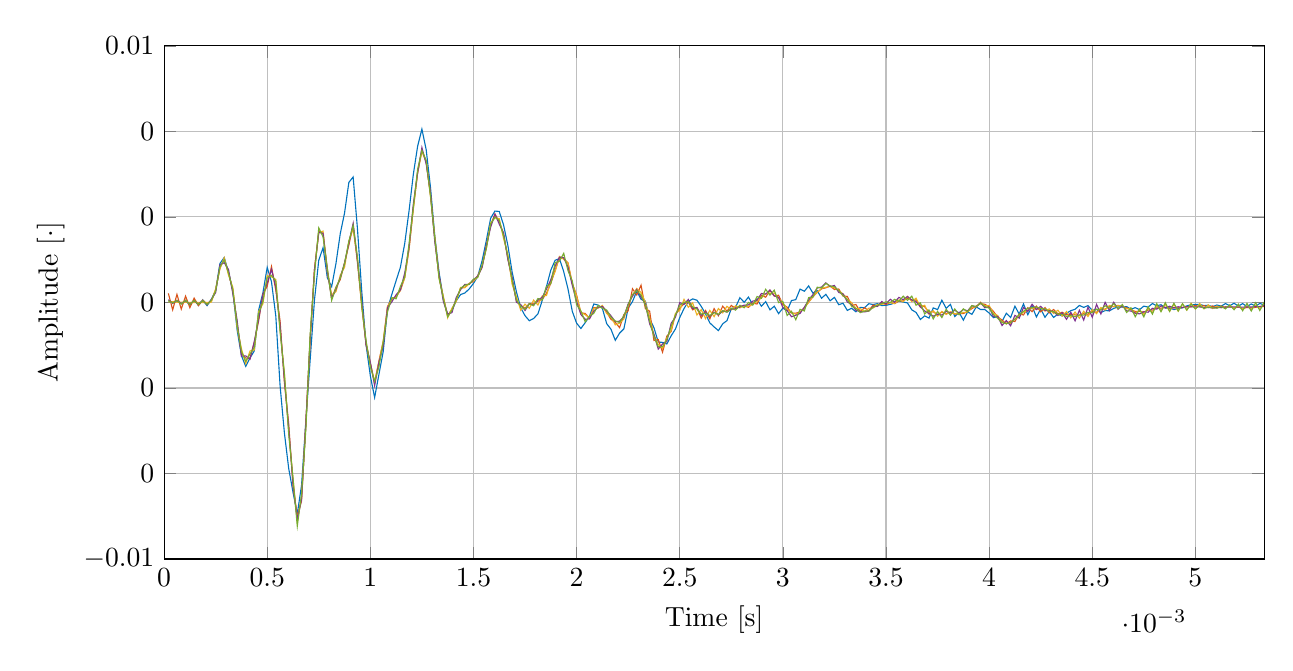
\begin{tikzpicture}

\begin{axis}[%
width=5.5in,
height=2.566in,
scaled y ticks = false,
y tick label style={/pgf/number format/fixed},
at={(0.758in,0.481in)},
scale only axis,
xmin=0,
xmax=0.005333,
xlabel={Time [s]},
xmajorgrids,
ymin=-0.006,
ymax=0.006,
ylabel={Amplitude [$\cdot$]},
ymajorgrids,
axis background/.style={fill=white},
legend style={legend cell align=left,align=left,draw=white!15!black}
]
\addplot [color=mycolor1,solid]
  table[row sep=crcr]{%
2.08333333333333e-05	1.3543391321508e-05\\
4.16666666666667e-05	1.04283477814182e-05\\
6.25e-05	3.44413334138925e-05\\
8.33333333333333e-05	-3.26787629992505e-05\\
0.000104166666666667	4.87962355574781e-05\\
0.000125	-6.27990621633765e-05\\
0.000145833333333333	5.77837048117993e-05\\
0.000166666666666667	-7.05936720947589e-05\\
0.0001875	5.96632997182354e-05\\
0.000208333333333333	-7.44801783974061e-05\\
0.000229166666666667	6.93026461959887e-05\\
0.00025	0.00028009617864295\\
0.000270833333333333	0.000910447245024445\\
0.000291666666666667	0.00104970501266502\\
0.0003125	0.000704760015325452\\
0.000333333333333333	0.000264053604856449\\
0.000354166666666667	-0.00064476195794403\\
0.000375	-0.00124338902711922\\
0.000395833333333333	-0.00149441025643127\\
0.000416666666666667	-0.00129889330975828\\
0.0004375	-0.00113228012067019\\
0.000458333333333333	-0.000180839240252783\\
0.000479166666666667	0.000223685595255964\\
0.0005	0.000818035990654932\\
0.000520833333333333	0.000481451461249429\\
0.000541666666666667	-0.000318070505195915\\
0.0005625	-0.00195147331246818\\
0.000583333333333333	-0.00305061541974597\\
0.000604166666666667	-0.00388069079363481\\
0.000625	-0.00443597787392001\\
0.000645833333333333	-0.00494724864934551\\
0.000666666666666667	-0.00426889454714502\\
0.0006875	-0.00276234544167092\\
0.000708333333333333	-0.00133565686874056\\
0.000729166666666667	5.69393625155881e-05\\
0.00075	0.000987660688631421\\
0.000770833333333333	0.00127893510967754\\
0.000791666666666667	0.000572944194756071\\
0.0008125	0.000369859578182828\\
0.000833333333333333	0.000910966047295416\\
0.000854166666666667	0.00160692743719571\\
0.000875	0.00209095091706099\\
0.000895833333333333	0.00280558893246012\\
0.000916666666666667	0.00293281257378255\\
0.0009375	0.00172664823869988\\
0.000958333333333333	0.000264215839549989\\
0.000979166666666667	-0.000988958569926658\\
0.001	-0.00171570400100181\\
0.00102083333333333	-0.00222302951794158\\
0.00104166666666667	-0.00168330692068448\\
0.0010625	-0.00114628371058388\\
0.00108333333333333	-0.000148573608889372\\
0.00110416666666667	0.000187259643228257\\
0.001125	0.000509272239150426\\
0.00114583333333333	0.0008232338864522\\
0.00116666666666667	0.00137789886038578\\
0.0011875	0.0021336498071616\\
0.00120833333333333	0.002990665986059\\
0.00122916666666667	0.00365029392969743\\
0.00125	0.00405221121651203\\
0.00127083333333333	0.00356842640516147\\
0.00129166666666667	0.00268895056091017\\
0.0013125	0.00155518471750718\\
0.00133333333333333	0.000701436313373912\\
0.00135416666666667	7.72712731343327e-05\\
0.001375	-0.000298244286176402\\
0.00139583333333333	-0.000181466811149252\\
0.00141666666666667	4.04369297374201e-05\\
0.0014375	0.000183869657917035\\
0.00145833333333333	0.000220238854362641\\
0.00147916666666667	0.000314669373974984\\
0.0015	0.00044475620056442\\
0.00152083333333333	0.000609519336366845\\
0.00154166666666667	0.000971648442995778\\
0.0015625	0.00145138769648321\\
0.00158333333333333	0.00196950196395125\\
0.00160416666666667	0.00213610661039513\\
0.001625	0.00212700460484258\\
0.00164583333333333	0.00181253129023513\\
0.00166666666666667	0.00133550584290811\\
0.0016875	0.000709502508390499\\
0.00170833333333333	0.000245043254398914\\
0.00172916666666667	-0.000125710768349654\\
0.00175	-0.00031017937620126\\
0.00177083333333333	-0.000428334719277469\\
0.00179166666666667	-0.00037505939234602\\
0.0018125	-0.00026892090302289\\
0.00183333333333333	4.60889606393628e-05\\
0.00185416666666667	0.000376130028157501\\
0.001875	0.000755722136329669\\
0.00189583333333333	0.000985496341933272\\
0.00191666666666667	0.00102471578137402\\
0.0019375	0.000719802860637036\\
0.00195833333333333	0.000314215506599397\\
0.00197916666666667	-0.000210027495432635\\
0.002	-0.000485097380700446\\
0.00202083333333333	-0.000609375993755614\\
0.00204166666666667	-0.000474043824591789\\
0.0020625	-0.000323003095865901\\
0.00208333333333333	-3.60620347955172e-05\\
0.00210416666666667	-6.16331425516677e-05\\
0.002125	-0.000140691942521645\\
0.00214583333333333	-0.00049631420429798\\
0.00216666666666667	-0.000627078009883062\\
0.0021875	-0.000886126597766334\\
0.00220833333333333	-0.00071850342674477\\
0.00222916666666667	-0.000617979955248239\\
0.00225	-0.000132398039957433\\
0.00227083333333333	1.82596795226726e-05\\
0.00229166666666667	0.000263457980795162\\
0.0023125	7.21701257126061e-05\\
0.00233333333333333	3.14696631696198e-05\\
0.00235416666666667	-0.000381908545746998\\
0.002375	-0.000591133646787553\\
0.00239583333333333	-0.000926931648229558\\
0.00241666666666667	-0.000934185888469817\\
0.0024375	-0.000971184740566583\\
0.00245833333333333	-0.000781897163411284\\
0.00247916666666667	-0.000621608190332199\\
0.0025	-0.000354517272005676\\
0.00252083333333333	-0.000142594728573159\\
0.00254166666666667	1.94955758899358e-05\\
0.0025625	8.27804421917184e-05\\
0.00258333333333333	5.16094935552072e-05\\
0.00260416666666667	-9.18614368237075e-05\\
0.002625	-0.000265049428279323\\
0.00264583333333333	-0.000478865678177664\\
0.00266666666666667	-0.000572778906941748\\
0.0026875	-0.000659181316702796\\
0.00270833333333333	-0.000500265460857302\\
0.00272916666666667	-0.000424943177290667\\
0.00275	-0.000145257330899531\\
0.00277083333333333	-0.000109887914112234\\
0.00279166666666667	0.000110193954462678\\
0.0028125	3.01018559284193e-06\\
0.00283333333333333	0.000124412895192399\\
0.00285416666666667	-5.26696911355543e-05\\
0.002875	7.51907209855034e-05\\
0.00289583333333333	-9.04152674633021e-05\\
0.00291666666666667	1.90371188900861e-05\\
0.0029375	-0.000173943600591536\\
0.00295833333333333	-8.84096434949333e-05\\
0.00297916666666667	-0.000262098030800291\\
0.003	-0.000133668837589748\\
0.00302083333333333	-0.000195957524195551\\
0.00304166666666667	4.32804477002738e-05\\
0.0030625	6.46657157793033e-05\\
0.00308333333333333	0.00031130794573477\\
0.00310416666666667	0.000260967272279442\\
0.003125	0.000385967312825046\\
0.00314583333333333	0.000216725487377815\\
0.00316666666666667	0.000275414513827533\\
0.0031875	9.83741710889995e-05\\
0.00320833333333333	0.000188703508985353\\
0.00322916666666667	3.93221899768309e-05\\
0.00325	0.00011786515214798\\
0.00327083333333333	-5.31954290621728e-05\\
0.00329166666666667	-1.89602478748384e-05\\
0.0033125	-0.000186363126657842\\
0.00333333333333333	-0.000136896921998522\\
0.00335416666666667	-0.000219207881294243\\
0.003375	-0.000116116027205388\\
0.00339583333333333	-0.000123983942307059\\
0.00341666666666667	-3.04884150285063e-05\\
0.0034375	-4.81949830765375e-05\\
0.00345833333333333	-2.91486025572701e-05\\
0.00347916666666667	-7.29474392611007e-05\\
0.0035	-6.72114193414311e-05\\
0.00352083333333333	-4.68101486328831e-05\\
0.00354166666666667	-1.27444626883886e-05\\
0.0035625	3.47996161603209e-05\\
0.00358333333333333	8.84517752463654e-06\\
0.00360416666666667	-1.22752956702464e-05\\
0.003625	-0.000173579753620194\\
0.00364583333333333	-0.000234484697253888\\
0.00366666666666667	-0.000398764315589376\\
0.0036875	-0.000314234900242703\\
0.00370833333333333	-0.000366677400081339\\
0.00372916666666667	-0.000128875782276004\\
0.00375	-0.000167353924003438\\
0.00377083333333333	5.14780220670528e-05\\
0.00379166666666667	-0.000137914673224701\\
0.0038125	-4.61484655575459e-05\\
0.00383333333333333	-0.00032885219441765\\
0.00385416666666667	-0.000229710003840824\\
0.003875	-0.000413907992495486\\
0.00389583333333333	-0.000221612572578095\\
0.00391666666666667	-0.000278608071414127\\
0.0039375	-0.000105407082810362\\
0.00395833333333333	-0.000165158409549793\\
0.00397916666666667	-0.000165056187709615\\
0.004	-0.000248280483288504\\
0.00402083333333333	-0.000356356930451698\\
0.00404166666666667	-0.00033209699388696\\
0.0040625	-0.000442700733465554\\
0.00408333333333333	-0.000253456677824533\\
0.00410416666666667	-0.000353035634181565\\
0.004125	-8.89736199120638e-05\\
0.00414583333333333	-0.000271643930209943\\
0.00416666666666667	-3.48091605270383e-05\\
0.0041875	-0.000288474294884654\\
0.00420833333333333	-8.7200443119657e-05\\
0.00422916666666667	-0.000339736640598831\\
0.00425	-0.000154834523602864\\
0.00427083333333333	-0.000347030321043853\\
0.00429166666666667	-0.000210674687236478\\
0.0043125	-0.000351559774509778\\
0.00433333333333333	-0.000273805789567957\\
0.00435416666666667	-0.000316322848767236\\
0.004375	-0.000251361301042229\\
0.00439583333333333	-0.000194042978172547\\
0.00441666666666667	-0.000159943477622711\\
0.0044375	-7.11365424094542e-05\\
0.00445833333333333	-0.000116321288412161\\
0.00447916666666667	-7.53051899015674e-05\\
0.0045	-0.000185282248725994\\
0.00452083333333333	-0.000161557409954925\\
0.00454166666666667	-0.000238844327680205\\
0.0045625	-0.000190398294782638\\
0.00458333333333333	-0.000196358474761996\\
0.00460416666666667	-0.000139240257839474\\
0.004625	-0.000106856056634805\\
0.00464583333333333	-0.000111803494155069\\
0.00466666666666667	-9.80798466338646e-05\\
0.0046875	-0.000158607859441535\\
0.00470833333333333	-0.000122256908439804\\
0.00472916666666667	-0.000169055261890888\\
0.00475	-8.64726427522868e-05\\
0.00477083333333333	-0.000110058019316055\\
0.00479166666666667	-2.63301192092538e-05\\
0.0048125	-7.8782665900775e-05\\
0.00483333333333333	-5.45149553755572e-05\\
0.00485416666666667	-0.000133712497165556\\
0.004875	-0.000125982170063066\\
0.00489583333333333	-0.000167918214879833\\
0.00491666666666667	-0.000138718157995903\\
0.0049375	-0.00012754022209929\\
0.00495833333333333	-8.06129133633587e-05\\
0.00497916666666667	-5.53906018964529e-05\\
0.005	-4.85068056612276e-05\\
0.00502083333333333	-4.66778724459454e-05\\
0.00504166666666667	-7.44187472976063e-05\\
0.0050625	-6.54976302909994e-05\\
0.00508333333333333	-0.000101062169659589\\
0.00510416666666667	-6.06949916458827e-05\\
0.005125	-8.77628766759077e-05\\
0.00514583333333333	-2.6561365812438e-05\\
0.00516666666666667	-7.64358658186436e-05\\
0.0051875	-1.91100806120724e-05\\
0.00520833333333333	-8.67845302082347e-05\\
0.00522916666666667	-2.75576980376769e-05\\
0.00525	-9.94566502819272e-05\\
0.00527083333333333	-3.52381999586357e-05\\
0.00529166666666667	-8.82347765157783e-05\\
0.0053125	-2.26685868456094e-05\\
0.00533333333333333	-6.26690991381589e-05\\
};
%\addlegendentry{Test1};

\addplot [color=mycolor2,solid]
  table[row sep=crcr]{%
2.08333333333333e-05	0.000211652413002886\\
4.16666666666667e-05	-0.000173339727002396\\
6.25e-05	0.000187750154651344\\
8.33333333333333e-05	-0.000156762459127076\\
0.000104166666666667	0.000147692174327862\\
0.000125	-0.000123329634108229\\
0.000145833333333333	9.99695936921326e-05\\
0.000166666666666667	-7.49370243406717e-05\\
0.0001875	5.47424640177845e-05\\
0.000208333333333333	-3.96691940819937e-05\\
0.000229166666666667	3.41590188913642e-05\\
0.00025	0.000294182951461304\\
0.000270833333333333	0.000806691732291888\\
0.000291666666666667	0.00101975509450399\\
0.0003125	0.000678937002734547\\
0.000333333333333333	0.000292360977688049\\
0.000354166666666667	-0.000501852124221478\\
0.000375	-0.00119285803437959\\
0.000395833333333333	-0.00130225366361762\\
0.000416666666666667	-0.00130604564558611\\
0.0004375	-0.00092828170951845\\
0.000458333333333333	-0.000432160595526375\\
0.000479166666666667	0.000190768499531546\\
0.0005	0.000377806122217988\\
0.000520833333333333	0.000840072590533338\\
0.000541666666666667	0.000284955296599346\\
0.0005625	-0.000432432141412539\\
0.000583333333333333	-0.00187434409663978\\
0.000604166666666667	-0.00282964897355679\\
0.000625	-0.00429030203522105\\
0.000645833333333333	-0.00500716086243622\\
0.000666666666666667	-0.00463815373049156\\
0.0006875	-0.00279301793664841\\
0.000708333333333333	-0.00087467507430674\\
0.000729166666666667	0.000765360638298775\\
0.00075	0.0016645902370319\\
0.000770833333333333	0.00161278876864379\\
0.000791666666666667	0.000778822164940748\\
0.0008125	8.95652765442366e-05\\
0.000833333333333333	0.000355994965932239\\
0.000854166666666667	0.000533142255648149\\
0.000875	0.000928225661844451\\
0.000895833333333333	0.00133842919064323\\
0.000916666666666667	0.00180432130887871\\
0.0009375	0.00092949915507937\\
0.000958333333333333	-5.48977050218582e-05\\
0.000979166666666667	-0.000988061762272893\\
0.001	-0.00141919557544236\\
0.00102083333333333	-0.00187978848327791\\
0.00104166666666667	-0.00136969624991704\\
0.0010625	-0.00091374530785761\\
0.00108333333333333	-9.52096710917287e-05\\
0.00110416666666667	8.14760798002777e-05\\
0.001125	0.000138323047384794\\
0.00114583333333333	0.000283276635588725\\
0.00116666666666667	0.000584630005377628\\
0.0011875	0.00123928141955519\\
0.00120833333333333	0.00219966968809687\\
0.00122916666666667	0.00302447517481785\\
0.00125	0.00356456277667745\\
0.00127083333333333	0.0032774611247043\\
0.00129166666666667	0.00252429204859592\\
0.0013125	0.00149598813446026\\
0.00133333333333333	0.000608034658739415\\
0.00135416666666667	0.00010710365299443\\
0.001375	-0.000311299309616197\\
0.00139583333333333	-0.000159692725767254\\
0.00141666666666667	5.74222657480503e-05\\
0.0014375	0.000332943796413054\\
0.00145833333333333	0.000354796163267122\\
0.00147916666666667	0.00044264717523641\\
0.0015	0.000490979136032597\\
0.00152083333333333	0.000627004516028203\\
0.00154166666666667	0.000823627273687755\\
0.0015625	0.00133148384003283\\
0.00158333333333333	0.00180538068202541\\
0.00160416666666667	0.0020679200528017\\
0.001625	0.00188089675493427\\
0.00164583333333333	0.00160050444426912\\
0.00166666666666667	0.00102528583093237\\
0.0016875	0.000530925221583447\\
0.00170833333333333	3.03588839609427e-05\\
0.00172916666666667	-6.96052972850161e-05\\
0.00175	-0.000138001487019424\\
0.00177083333333333	-2.65371796825528e-05\\
0.00179166666666667	-3.37410928485125e-05\\
0.0018125	2.80864752783102e-05\\
0.00183333333333333	7.1940834481178e-05\\
0.00185416666666667	0.000216995882119329\\
0.001875	0.000446510022235784\\
0.00189583333333333	0.000748772029844977\\
0.00191666666666667	0.00104142044629439\\
0.0019375	0.00102571534353267\\
0.00195833333333333	0.000920887069273338\\
0.00197916666666667	0.000441857008437858\\
0.002	0.000170462647395816\\
0.00202083333333333	-0.000241902785740941\\
0.00204166666666667	-0.000258455926668494\\
0.0020625	-0.000374322087367231\\
0.00208333333333333	-0.000121925548494941\\
0.00210416666666667	-0.000127018713507529\\
0.002125	-8.89672524345951e-05\\
0.00214583333333333	-0.000233276979776478\\
0.00216666666666667	-0.000395760659992537\\
0.0021875	-0.000466155327677042\\
0.00220833333333333	-0.000589933471176561\\
0.00222916666666667	-0.000284518446553593\\
0.00225	-0.000196559976575267\\
0.00227083333333333	0.000319435821748174\\
0.00229166666666667	0.000174867526418859\\
0.0023125	0.000402327459949324\\
0.00233333333333333	-0.000145509644797631\\
0.00235416666666667	-0.00020421993760988\\
0.002375	-0.000890458264656727\\
0.00239583333333333	-0.000865555679928417\\
0.00241666666666667	-0.0011629971069399\\
0.0024375	-0.000787739864021896\\
0.00245833333333333	-0.000677882106135698\\
0.00247916666666667	-0.000283459591626764\\
0.0025	-0.000136853741907463\\
0.00252083333333333	-3.06559579855046e-05\\
0.00254166666666667	5.55181821134803e-06\\
0.0025625	-0.00017290845570517\\
0.00258333333333333	-0.000127871429654874\\
0.00260416666666667	-0.000367288284586136\\
0.002625	-0.000189460307003649\\
0.00264583333333333	-0.000384996067923299\\
0.00266666666666667	-0.000145803163555069\\
0.0026875	-0.00030991705336988\\
0.00270833333333333	-8.80489758752125e-05\\
0.00272916666666667	-0.000206718236570388\\
0.00275	-7.09295178031552e-05\\
0.00277083333333333	-0.000139373242028403\\
0.00279166666666667	-8.95453807616241e-05\\
0.0028125	-8.4625509795232e-05\\
0.00283333333333333	-0.0001142217764346\\
0.00285416666666667	-1.44587330440699e-05\\
0.002875	-3.8489977866137e-05\\
0.00289583333333333	0.000164483523204615\\
0.00291666666666667	0.000121618650855541\\
0.0029375	0.000282754260002095\\
0.00295833333333333	0.000148969724663405\\
0.00297916666666667	0.000168024195960275\\
0.003	-4.94379860644293e-05\\
0.00302083333333333	-0.000110898023493295\\
0.00304166666666667	-0.000249816634906391\\
0.0030625	-0.000250556662212618\\
0.00308333333333333	-0.000225324708049882\\
0.00310416666666667	-0.00012662378841728\\
0.003125	1.10856436103505e-05\\
0.00314583333333333	0.000130429633316803\\
0.00316666666666667	0.000237537683408878\\
0.0031875	0.000317552073843242\\
0.00320833333333333	0.000341515697311883\\
0.00322916666666667	0.00038314005268002\\
0.00325	0.000301660034364847\\
0.00327083333333333	0.000313715872706783\\
0.00329166666666667	0.000146113367877221\\
0.0033125	0.000141723283462845\\
0.00333333333333333	-7.02996928949661e-05\\
0.00335416666666667	-4.94105315210008e-05\\
0.003375	-0.000215554265462105\\
0.00339583333333333	-0.000123590944566932\\
0.00341666666666667	-0.000198347977769429\\
0.0034375	-6.1026419394519e-05\\
0.00345833333333333	-9.4637359807703e-05\\
0.00347916666666667	-3.85826214154908e-06\\
0.0035	-5.12980259859393e-05\\
0.00352083333333333	9.06307448279722e-07\\
0.00354166666666667	-2.83100555675652e-05\\
0.0035625	3.39520507851667e-05\\
0.00358333333333333	3.63621669502733e-05\\
0.00360416666666667	0.000100542387778045\\
0.003625	5.99220845705767e-05\\
0.00364583333333333	5.63850588164025e-05\\
0.00366666666666667	-6.51801823260267e-05\\
0.0036875	-0.000102207667044161\\
0.00370833333333333	-0.0002287997126078\\
0.00372916666666667	-0.000217708066739107\\
0.00375	-0.000284105541481261\\
0.00377083333333333	-0.00022535641267432\\
0.00379166666666667	-0.000263973420817005\\
0.0038125	-0.000226420230010242\\
0.00383333333333333	-0.000272255435322869\\
0.00385416666666667	-0.000260280919211489\\
0.003875	-0.000260716752357806\\
0.00389583333333333	-0.00021206882715147\\
0.00391666666666667	-0.000143541375603385\\
0.0039375	-8.25053161878263e-05\\
0.00395833333333333	-2.87892519682763e-05\\
0.00397916666666667	-4.28102119928965e-05\\
0.004	-0.00010353474872191\\
0.00402083333333333	-0.000208590095915721\\
0.00404166666666667	-0.000342617077010653\\
0.0040625	-0.000410779771190247\\
0.00408333333333333	-0.000503702536118708\\
0.00410416666666667	-0.000432197883153678\\
0.004125	-0.00044640086638442\\
0.00414583333333333	-0.000269549299251874\\
0.00416666666666667	-0.000292926780043726\\
0.0041875	-0.000123516150214578\\
0.00420833333333333	-0.000215279138016835\\
0.00422916666666667	-8.73021214159691e-05\\
0.00425	-0.000219110831361126\\
0.00427083333333333	-0.00011976663824827\\
0.00429166666666667	-0.00024448538527706\\
0.0043125	-0.000166553342858026\\
0.00433333333333333	-0.000269208408656361\\
0.00435416666666667	-0.000229108881912949\\
0.004375	-0.000291480490023811\\
0.00439583333333333	-0.000276707457881946\\
0.00441666666666667	-0.000292300924758533\\
0.0044375	-0.000298125311117598\\
0.00445833333333333	-0.000264760478439086\\
0.00447916666666667	-0.00027640820233766\\
0.0045	-0.000212008308381538\\
0.00452083333333333	-0.00022938167725134\\
0.00454166666666667	-0.000151744559736019\\
0.0045625	-0.000158743606101135\\
0.00458333333333333	-8.67537917035841e-05\\
0.00460416666666667	-9.79344349253515e-05\\
0.004625	-6.97440102684591e-05\\
0.00464583333333333	-9.94351075181312e-05\\
0.00466666666666667	-0.000126950588252781\\
0.0046875	-0.000166269097157796\\
0.00470833333333333	-0.000213419709527198\\
0.00472916666666667	-0.000209952140014507\\
0.00475	-0.000225526703780452\\
0.00477083333333333	-0.000178073057224544\\
0.00479166666666667	-0.000178683618755746\\
0.0048125	-0.00012596683847686\\
0.00483333333333333	-0.00013573004894371\\
0.00485416666666667	-0.000113435090528345\\
0.004875	-0.00013625018241199\\
0.00489583333333333	-0.000126165302621157\\
0.00491666666666667	-0.000126958157364084\\
0.0049375	-0.000118825453594291\\
0.00495833333333333	-9.94401918595839e-05\\
0.00497916666666667	-0.000101331854539892\\
0.005	-7.17359294125052e-05\\
0.00502083333333333	-0.000100811822131616\\
0.00504166666666667	-7.49247091332742e-05\\
0.0050625	-0.000119259307923103\\
0.00508333333333333	-8.14335112199732e-05\\
0.00510416666666667	-0.000127378224874349\\
0.005125	-8.19365777125725e-05\\
0.00514583333333333	-0.000127072485066847\\
0.00516666666666667	-8.50501570915194e-05\\
0.0051875	-0.000133880041625743\\
0.00520833333333333	-0.000106768634559069\\
0.00522916666666667	-0.000142994721170173\\
0.00525	-0.000118739090511832\\
0.00527083333333333	-0.000128582608997943\\
0.00529166666666667	-0.000115359420085285\\
0.0053125	-9.41890279160041e-05\\
0.00533333333333333	-9.77463031800505e-05\\
};
%\addlegendentry{Test2};

\addplot [color=mycolor3,solid]
  table[row sep=crcr]{%
2.08333333333333e-05	8.79099582887213e-06\\
4.16666666666667e-05	1.93077100801325e-05\\
6.25e-05	3.80102871329913e-06\\
8.33333333333333e-05	7.28870620084327e-06\\
0.000104166666666667	-2.2944670425061e-07\\
0.000125	-1.14161126662867e-06\\
0.000145833333333333	-2.34347657156573e-06\\
0.000166666666666667	1.92038851230251e-06\\
0.0001875	-3.24994437830764e-06\\
0.000208333333333333	4.83707566340526e-07\\
0.000229166666666667	6.14979132268234e-06\\
0.00025	0.000314582523351701\\
0.000270833333333333	0.000784409768559453\\
0.000291666666666667	0.00104440303970656\\
0.0003125	0.000638237968299054\\
0.000333333333333333	0.000351199319975806\\
0.000354166666666667	-0.00058005497501085\\
0.000375	-0.00108063310093185\\
0.000395833333333333	-0.0014308631924099\\
0.000416666666666667	-0.00113557425375637\\
0.0004375	-0.00111111318667703\\
0.000458333333333333	-0.000211985074964642\\
0.000479166666666667	-3.28130601543212e-05\\
0.0005	0.000625754180927256\\
0.000520833333333333	0.000599305717774156\\
0.000541666666666667	0.000535836424513515\\
0.0005625	-0.000657279133892127\\
0.000583333333333333	-0.00164602856697408\\
0.000604166666666667	-0.00300789396159314\\
0.000625	-0.00410841612347663\\
0.000645833333333333	-0.00512294229721497\\
0.000666666666666667	-0.00452639003522694\\
0.0006875	-0.00284542817169532\\
0.000708333333333333	-0.000842456856295743\\
0.000729166666666667	0.000770445407705592\\
0.00075	0.00162743267489224\\
0.000770833333333333	0.00166816090211969\\
0.000791666666666667	0.0006954934989472\\
0.0008125	0.000180033178744993\\
0.000833333333333333	0.000249198493917309\\
0.000854166666666667	0.000637969713402775\\
0.000875	0.000820070938212411\\
0.000895833333333333	0.0014394804225797\\
0.000916666666666667	0.00171424844140245\\
0.0009375	0.00101645824474284\\
0.000958333333333333	-0.000116427220567084\\
0.000979166666666667	-0.000924314311471324\\
0.001	-0.00145469383580713\\
0.00102083333333333	-0.00184603675929653\\
0.00104166666666667	-0.00139060466423514\\
0.0010625	-0.000908639655509855\\
0.00108333333333333	-0.000108900276376925\\
0.00110416666666667	7.57691270635511e-05\\
0.001125	0.000131496637675384\\
0.00114583333333333	0.000282218352033241\\
0.00116666666666667	0.000578562889487158\\
0.0011875	0.00124884055345609\\
0.00120833333333333	0.00217985349932865\\
0.00122916666666667	0.003036104914506\\
0.00125	0.0035236477953967\\
0.00127083333333333	0.00329562573991942\\
0.00129166666666667	0.00247318738079894\\
0.0013125	0.00152336922848473\\
0.00133333333333333	0.000554550349390318\\
0.00135416666666667	0.000138284131101107\\
0.001375	-0.000359856674798715\\
0.00139583333333333	-0.000132317615591518\\
0.00141666666666667	2.35848573199566e-05\\
0.0014375	0.000350524551556039\\
0.00145833333333333	0.000341994426939455\\
0.00147916666666667	0.000438764508668613\\
0.0015	0.000500190035370381\\
0.00152083333333333	0.000593286937970453\\
0.00154166666666667	0.000855466355535522\\
0.0015625	0.00126726096756404\\
0.00158333333333333	0.00185980528587988\\
0.00160416666666667	0.00197657245349987\\
0.001625	0.00195739871311337\\
0.00164583333333333	0.00149502081460735\\
0.00166666666666667	0.00112426398184831\\
0.0016875	0.000420458245890128\\
0.00170833333333333	0.000137059782379609\\
0.00172916666666667	-0.000183789139879221\\
0.00175	-3.93577010889362e-05\\
0.00177083333333333	-0.000137400962018175\\
0.00179166666666667	5.32155626485968e-05\\
0.0018125	-6.06506151678888e-05\\
0.00183333333333333	0.000150657983096565\\
0.00185416666666667	0.000161327673496062\\
0.001875	0.000510398112082594\\
0.00189583333333333	0.000718589786001642\\
0.00191666666666667	0.00107401802269619\\
0.0019375	0.00100893947054841\\
0.00195833333333333	0.000920844696813718\\
0.00197916666666667	0.000436220555090565\\
0.002	0.000149080333323178\\
0.00202083333333333	-0.000239144956464202\\
0.00204166666666667	-0.000284767071535052\\
0.0020625	-0.000369858810550623\\
0.00208333333333333	-0.00013496156980077\\
0.00210416666666667	-0.000131775858176881\\
0.002125	-7.18273139731866e-05\\
0.00214583333333333	-0.000259490661349661\\
0.00216666666666667	-0.000335916806072985\\
0.0021875	-0.000525433293299304\\
0.00220833333333333	-0.000485154366056565\\
0.00222916666666667	-0.000386196277685327\\
0.00225	-5.78934869298038e-05\\
0.00227083333333333	0.000174099594820086\\
0.00229166666666667	0.000327818706767721\\
0.0023125	0.000231533673155345\\
0.00233333333333333	5.71964629770565e-06\\
0.00235416666666667	-0.000364307767173939\\
0.002375	-0.000758202460161561\\
0.00239583333333333	-0.000979855422085915\\
0.00241666666666667	-0.0010725901676377\\
0.0024375	-0.000834790885168691\\
0.00245833333333333	-0.000653607403373683\\
0.00247916666666667	-0.000255395400238981\\
0.0025	-0.000188408814105637\\
0.00252083333333333	7.08540772785519e-05\\
0.00254166666666667	-0.000113271794792744\\
0.0025625	-9.86319036822128e-06\\
0.00258333333333333	-0.00029388085852394\\
0.00260416666666667	-0.000169725489253644\\
0.002625	-0.000377868452111989\\
0.00264583333333333	-0.000186793737461812\\
0.00266666666666667	-0.000331788866956558\\
0.0026875	-0.000143791264575545\\
0.00270833333333333	-0.000245062633392467\\
0.00272916666666667	-9.11962267637011e-05\\
0.00275	-0.000174568537646461\\
0.00277083333333333	-7.88460993435035e-05\\
0.00279166666666667	-0.000127804008335698\\
0.0028125	-7.50735399017756e-05\\
0.00283333333333333	-9.24119973535204e-05\\
0.00285416666666667	-4.61852128210986e-05\\
0.002875	2.60643181313603e-05\\
0.00289583333333333	0.000105938467912551\\
0.00291666666666667	0.00020224818082826\\
0.0029375	0.000214019845901123\\
0.00295833333333333	0.000219811279516083\\
0.00297916666666667	0.000102409482690558\\
0.003	-7.10745574568076e-06\\
0.00302083333333333	-0.00016038728826776\\
0.00304166666666667	-0.000238233445508772\\
0.0030625	-0.00027473145931691\\
0.00308333333333333	-0.000233879501172097\\
0.00310416666666667	-0.000124651940532275\\
0.003125	-1.53570071449187e-06\\
0.00314583333333333	0.000146441714633855\\
0.00316666666666667	0.00023342992818712\\
0.0031875	0.000328630282268613\\
0.00320833333333333	0.00035517772735928\\
0.00322916666666667	0.000372023886993519\\
0.00325	0.000336713311015084\\
0.00327083333333333	0.000271020980970166\\
0.00329166666666667	0.000200357432768382\\
0.0033125	6.93581078434166e-05\\
0.00333333333333333	-4.21573270597202e-06\\
0.00335416666666667	-0.00013901998310668\\
0.003375	-0.000145882619422008\\
0.00339583333333333	-0.000212107489527447\\
0.00341666666666667	-0.000135384157598845\\
0.0034375	-0.000130767895747932\\
0.00345833333333333	-4.70617344647251e-05\\
0.00347916666666667	-4.38033223644162e-05\\
0.0035	-2.48962021834155e-05\\
0.00352083333333333	-4.22992252715018e-06\\
0.00354166666666667	-2.49002497487254e-05\\
0.0035625	5.86241513355626e-05\\
0.00358333333333333	1.69953607525617e-05\\
0.00360416666666667	0.00014188537407565\\
0.003625	2.07243789569665e-05\\
0.00364583333333333	9.94594825175192e-05\\
0.00366666666666667	-0.000116641733083839\\
0.0036875	-6.67884065453506e-05\\
0.00370833333333333	-0.000279736200287731\\
0.00372916666666667	-0.000192974293274063\\
0.00375	-0.000321944862836492\\
0.00377083333333333	-0.000210615960144979\\
0.00379166666666667	-0.000280418385257635\\
0.0038125	-0.000220022400553348\\
0.00383333333333333	-0.000265969146379116\\
0.00385416666666667	-0.000261732609565939\\
0.003875	-0.000236977097971416\\
0.00389583333333333	-0.000222979460389728\\
0.00391666666666667	-0.000111735065562769\\
0.0039375	-0.000106049901013329\\
0.00395833333333333	3.88804375199628e-06\\
0.00397916666666667	-7.96284067164368e-05\\
0.004	-7.20492776729357e-05\\
0.00402083333333333	-0.000256522844237608\\
0.00404166666666667	-0.0003074977038931\\
0.0040625	-0.000464599651550528\\
0.00408333333333333	-0.000458335855230529\\
0.00410416666666667	-0.000489818574842899\\
0.004125	-0.000386685560497293\\
0.00414583333333333	-0.000331132097109103\\
0.00416666666666667	-0.00021936578984871\\
0.0041875	-0.000191612495580438\\
0.00420833333333333	-0.000129678536141437\\
0.00422916666666667	-0.000162963528337683\\
0.00425	-0.000126710219973669\\
0.00427083333333333	-0.000203273940453631\\
0.00429166666666667	-0.00015162219086902\\
0.0043125	-0.000256187301599867\\
0.00433333333333333	-0.000182531200835043\\
0.00435416666666667	-0.000319741828108128\\
0.004375	-0.000213951147486418\\
0.00439583333333333	-0.000361027627948987\\
0.00441666666666667	-0.00022484324398039\\
0.0044375	-0.000368690199756786\\
0.00445833333333333	-0.00020702457084678\\
0.00447916666666667	-0.000328764161960882\\
0.0045	-0.000164946510966098\\
0.00452083333333333	-0.000262854983870519\\
0.00454166666666667	-0.000118142333069678\\
0.0045625	-0.000175292676674079\\
0.00458333333333333	-7.0518396509314e-05\\
0.00460416666666667	-9.99356250500361e-05\\
0.004625	-7.31960072618698e-05\\
0.00464583333333333	-8.92814792055228e-05\\
0.00466666666666667	-0.00015073023639968\\
0.0046875	-0.000144384882629013\\
0.00470833333333333	-0.000254916817986933\\
0.00472916666666667	-0.00017516458926567\\
0.00475	-0.000279802125903244\\
0.00477083333333333	-0.000129340318403991\\
0.00479166666666667	-0.000240907998723586\\
0.0048125	-6.38364050541188e-05\\
0.00483333333333333	-0.000203163314147123\\
0.00485416666666667	-3.98917154711702e-05\\
0.004875	-0.000208597442647207\\
0.00489583333333333	-4.47974225922933e-05\\
0.00491666666666667	-0.000204084342770989\\
0.0049375	-3.47872183795294e-05\\
0.00495833333333333	-0.000180487695375069\\
0.00497916666666667	-1.9689397009039e-05\\
0.005	-0.000152786199350786\\
0.00502083333333333	-2.7096589687821e-05\\
0.00504166666666667	-0.000149690765436414\\
0.0050625	-5.88093667115747e-05\\
0.00508333333333333	-0.000142545580482899\\
0.00510416666666667	-8.42705370601839e-05\\
0.005125	-0.000123542444792071\\
0.00514583333333333	-0.00010250580870797\\
0.00516666666666667	-0.000103048012070152\\
0.0051875	-0.000127406740633103\\
0.00520833333333333	-0.000101375763624332\\
0.00522916666666667	-0.00015318481864193\\
0.00525	-9.23476302718807e-05\\
0.00527083333333333	-0.000155605621571469\\
0.00529166666666667	-7.25349055346226e-05\\
0.0053125	-0.000137762419270005\\
0.00533333333333333	-4.23257923087522e-05\\
};
%\addlegendentry{Test3};

\addplot [color=mycolor4,solid]
  table[row sep=crcr]{%
2.08333333333333e-05	6.46183523905331e-05\\
4.16666666666667e-05	-2.43787334953053e-05\\
6.25e-05	4.73731263489139e-05\\
8.33333333333333e-05	-2.60204072021243e-05\\
0.000104166666666667	3.44237892315021e-05\\
0.000125	-3.11910128314552e-05\\
0.000145833333333333	3.11257095003749e-05\\
0.000166666666666667	-3.63057614848314e-05\\
0.0001875	3.93164813204379e-05\\
0.000208333333333333	-5.7395230987016e-05\\
0.000229166666666667	6.94220693025882e-05\\
0.00025	0.000228846483619945\\
0.000270833333333333	0.000877629119787172\\
0.000291666666666667	0.000928492997504373\\
0.0003125	0.000767767731661118\\
0.000333333333333333	0.00020177870413226\\
0.000354166666666667	-0.000419987452889015\\
0.000375	-0.0012570510199655\\
0.000395833333333333	-0.00124959064785319\\
0.000416666666666667	-0.00132872794071519\\
0.0004375	-0.00091321682388105\\
0.000458333333333333	-0.000397025085610388\\
0.000479166666666667	0.000168540613570321\\
0.0005	0.00045047919202313\\
0.000520833333333333	0.00077056625060232\\
0.000541666666666667	0.000358984153730541\\
0.0005625	-0.000542903561873053\\
0.000583333333333333	-0.00180395400738984\\
0.000604166666666667	-0.00293258899567266\\
0.000625	-0.00423156312527304\\
0.000645833333333333	-0.00508311537692289\\
0.000666666666666667	-0.00459360343032139\\
0.0006875	-0.00281815565111528\\
0.000708333333333333	-0.000854437877356298\\
0.000729166666666667	0.000761263118676403\\
0.00075	0.001637678877443\\
0.000770833333333333	0.00161558615610072\\
0.000791666666666667	0.000717658650973874\\
0.0008125	9.86516512494268e-05\\
0.000833333333333333	0.000309158501573408\\
0.000854166666666667	0.000578910911477279\\
0.000875	0.000919023282167928\\
0.000895833333333333	0.0013943438473775\\
0.000916666666666667	0.00184771205392087\\
0.0009375	0.000991596941196099\\
0.000958333333333333	2.05922316863067e-06\\
0.000979166666666667	-0.000979443103589575\\
0.001	-0.00139779229673998\\
0.00102083333333333	-0.00194642800235158\\
0.00104166666666667	-0.00139937404827995\\
0.0010625	-0.00102610032673771\\
0.00108333333333333	-0.000121982006694414\\
0.00110416666666667	1.39077091186166e-05\\
0.001125	0.000179326661638432\\
0.00114583333333333	0.000291646317143645\\
0.00116666666666667	0.000683931426244691\\
0.0011875	0.0012848301112969\\
0.00120833333333333	0.00229553120744038\\
0.00122916666666667	0.00302896334526293\\
0.00125	0.00362026340634884\\
0.00127083333333333	0.00323607784935581\\
0.00129166666666667	0.00255670919957308\\
0.0013125	0.00141613594919881\\
0.00133333333333333	0.000634939332350084\\
0.00135416666666667	1.76153420127628e-05\\
0.001375	-0.000275756178071408\\
0.00139583333333333	-0.000237498394623217\\
0.00141666666666667	0.000118500024764612\\
0.0014375	0.000297779325538975\\
0.00145833333333333	0.000423218642033225\\
0.00147916666666667	0.000422686735566435\\
0.0015	0.000531860431389776\\
0.00152083333333333	0.000612856134672993\\
0.00154166666666667	0.000819755697528746\\
0.0015625	0.00131155196759777\\
0.00158333333333333	0.00176073111521903\\
0.00160416666666667	0.00206038406813562\\
0.001625	0.00183166554868252\\
0.00164583333333333	0.00163068436850075\\
0.00166666666666667	0.00100426480465606\\
0.0016875	0.000583840466842803\\
0.00170833333333333	3.60846214545357e-06\\
0.00172916666666667	-5.04250190357848e-05\\
0.00175	-0.000188493224407972\\
0.00177083333333333	-3.21610661486808e-05\\
0.00179166666666667	-6.15826302757681e-05\\
0.0018125	5.90645261311661e-05\\
0.00183333333333333	0.000116924997300413\\
0.00185416666666667	0.000314117948901296\\
0.001875	0.000529304233463109\\
0.00189583333333333	0.000846180196935928\\
0.00191666666666667	0.00105862512193366\\
0.0019375	0.00104705359395305\\
0.00195833333333333	0.000824856384428375\\
0.00197916666666667	0.000397351400609007\\
0.002	1.80067149112744e-05\\
0.00202083333333333	-0.000284026308090257\\
0.00204166666666667	-0.000393862638718029\\
0.0020625	-0.000383654780054348\\
0.00208333333333333	-0.000204171394180252\\
0.00210416666666667	-0.000109271471604404\\
0.002125	-9.39630334402072e-05\\
0.00214583333333333	-0.000202683551877193\\
0.00216666666666667	-0.000312639175296806\\
0.0021875	-0.000451283093602559\\
0.00220833333333333	-0.000439267118074206\\
0.00222916666666667	-0.00033785268420618\\
0.00225	-3.65316982332345e-05\\
0.00227083333333333	0.000144750096385841\\
0.00229166666666667	0.000300161092297901\\
0.0023125	0.000124090018900786\\
0.00233333333333333	-3.41535752983602e-05\\
0.00235416666666667	-0.000500547701567812\\
0.002375	-0.000745541988874006\\
0.00239583333333333	-0.00109129217811471\\
0.00241666666666667	-0.000970803582350909\\
0.0024375	-0.000915935472329271\\
0.00245833333333333	-0.000488844737093248\\
0.00247916666666667	-0.000344805694329203\\
0.0025	-6.10840393187385e-06\\
0.00252083333333333	-4.57926214945406e-05\\
0.00254166666666667	6.94841837154575e-05\\
0.0025625	-0.000141377645346978\\
0.00258333333333333	-0.000116621604357621\\
0.00260416666666667	-0.000302935413185849\\
0.002625	-0.000221240100232966\\
0.00264583333333333	-0.000325720296708212\\
0.00266666666666667	-0.000227772418535108\\
0.0026875	-0.000293746134299171\\
0.00270833333333333	-0.000199072801544017\\
0.00272916666666667	-0.000224806796374847\\
0.00275	-0.000157870403924333\\
0.00277083333333333	-0.000150365442992749\\
0.00279166666666667	-0.000103550276509605\\
0.0028125	-6.37338085997016e-05\\
0.00283333333333333	-5.8552139254128e-05\\
0.00285416666666667	3.0438996291179e-05\\
0.002875	5.36758642499138e-05\\
0.00289583333333333	0.000208302020145207\\
0.00291666666666667	0.000194426922535445\\
0.0029375	0.000290184341727993\\
0.00295833333333333	0.000154114165514923\\
0.00297916666666667	0.000117095863465312\\
0.003	-0.000117968216929227\\
0.00302083333333333	-0.000190444899907099\\
0.00304166666666667	-0.000334744961174545\\
0.0030625	-0.000300685747787608\\
0.00308333333333333	-0.000257223182107339\\
0.00310416666666667	-0.000112809519368785\\
0.003125	5.75509755873685e-05\\
0.00314583333333333	0.000182061781283863\\
0.00316666666666667	0.000337435786215885\\
0.0031875	0.000358836972369403\\
0.00320833333333333	0.000456144054099213\\
0.00322916666666667	0.000371078974361768\\
0.00325	0.000395160514956065\\
0.00327083333333333	0.000233851344109432\\
0.00329166666666667	0.000200320191247591\\
0.0033125	1.20605761718204e-05\\
0.00333333333333333	-5.15785023967148e-05\\
0.00335416666666667	-0.000185267810610958\\
0.003375	-0.00021544497629107\\
0.00339583333333333	-0.000222319799711762\\
0.00341666666666667	-0.000200626931157473\\
0.0034375	-9.90575514883635e-05\\
0.00345833333333333	-9.20129646790785e-05\\
0.00347916666666667	2.01437634022588e-05\\
0.0035	-3.38566169251028e-05\\
0.00352083333333333	7.34525461807813e-05\\
0.00354166666666667	4.92901559176769e-06\\
0.0035625	0.000117006640835086\\
0.00358333333333333	6.47564527164976e-05\\
0.00360416666666667	0.000137842316543066\\
0.003625	5.53331969583421e-05\\
0.00364583333333333	1.54099811552419e-05\\
0.00366666666666667	-0.000100401110229312\\
0.0036875	-0.000201181247736883\\
0.00370833333333333	-0.000258062802331095\\
0.00372916666666667	-0.00032249119346418\\
0.00375	-0.000273555649304275\\
0.00377083333333333	-0.000296523294570668\\
0.00379166666666667	-0.000205168909661912\\
0.0038125	-0.000249915864330484\\
0.00383333333333333	-0.000181144681833824\\
0.00385416666666667	-0.000249152787686495\\
0.003875	-0.000164965566937649\\
0.00389583333333333	-0.000197638190447784\\
0.00391666666666667	-7.72420908933912e-05\\
0.0039375	-0.000105944980589659\\
0.00395833333333333	-6.72514136803577e-06\\
0.00397916666666667	-0.000123535254728506\\
0.004	-0.000109103464312473\\
0.00402083333333333	-0.000331859311070721\\
0.00404166666666667	-0.000325441760158902\\
0.0040625	-0.000540008587551029\\
0.00408333333333333	-0.000424969414334501\\
0.00410416666666667	-0.000545809588056399\\
0.004125	-0.000302705444859084\\
0.00414583333333333	-0.000367603215795576\\
0.00416666666666667	-0.000116169946308302\\
0.0041875	-0.000212557370088295\\
0.00420833333333333	-4.27840820850104e-05\\
0.00422916666666667	-0.00016713387928269\\
0.00425	-9.13835008668613e-05\\
0.00427083333333333	-0.000187839813649044\\
0.00429166666666667	-0.000192668685064333\\
0.0043125	-0.00021673556295414\\
0.00433333333333333	-0.000304754020933578\\
0.00435416666666667	-0.000242193970524045\\
0.004375	-0.000395159595457167\\
0.00439583333333333	-0.000230514078343464\\
0.00441666666666667	-0.000431812596073038\\
0.0044375	-0.000183656367566198\\
0.00445833333333333	-0.000411116084422686\\
0.00447916666666667	-0.000109657519639442\\
0.0045	-0.000347793550913145\\
0.00452083333333333	-4.47532786439588e-05\\
0.00454166666666667	-0.000269891804051423\\
0.0045625	2.8457154577109e-06\\
0.00458333333333333	-0.000188127035822441\\
0.00460416666666667	3.84655355763523e-06\\
0.004625	-0.000158559664340847\\
0.00464583333333333	-7.30136597857576e-05\\
0.00466666666666667	-0.000197763109066923\\
0.0046875	-0.000199745806113596\\
0.00470833333333333	-0.000251407059669715\\
0.00472916666666667	-0.000267461731345711\\
0.00475	-0.000219579551603069\\
0.00477083333333333	-0.000229260236514911\\
0.00479166666666667	-0.000137834481557078\\
0.0048125	-0.00015745002679461\\
0.00483333333333333	-8.04604323346505e-05\\
0.00485416666666667	-0.000127033770706702\\
0.004875	-8.85753477233711e-05\\
0.00489583333333333	-0.000126930224281121\\
0.00491666666666667	-0.000101528913348219\\
0.0049375	-0.000117568468534481\\
0.00495833333333333	-0.000104499016945273\\
0.00497916666666667	-0.000102933919354474\\
0.005	-0.000102814263842561\\
0.00502083333333333	-0.000104325639340299\\
0.00504166666666667	-0.000120905242265535\\
0.0050625	-0.000118510592889796\\
0.00508333333333333	-0.000129081709012621\\
0.00510416666666667	-0.000118450252840674\\
0.005125	-0.0001219773335393\\
0.00514583333333333	-0.000106855792178922\\
0.00516666666666667	-0.000109344825883532\\
0.0051875	-0.000103732296601568\\
0.00520833333333333	-0.000111665608818279\\
0.00522916666666667	-0.000109090759927966\\
0.00525	-0.000107343590458587\\
0.00527083333333333	-0.0001066947340877\\
0.00529166666666667	-9.51112147065228e-05\\
0.0053125	-9.89199674438818e-05\\
0.00533333333333333	-7.33851628849622e-05\\
};
%\addlegendentry{Test4};

\addplot [color=mycolor5,solid]
  table[row sep=crcr]{%
2.08333333333333e-05	4.15176990932612e-05\\
4.16666666666667e-05	-1.53728983876088e-05\\
6.25e-05	4.82170803430168e-05\\
8.33333333333333e-05	-3.72467666418004e-05\\
0.000104166666666667	4.88734755992583e-05\\
0.000125	-4.91927240729155e-05\\
0.000145833333333333	4.64487683936852e-05\\
0.000166666666666667	-4.62713439802019e-05\\
0.0001875	4.18795743562836e-05\\
0.000208333333333333	-4.75578682651901e-05\\
0.000229166666666667	4.81102517219336e-05\\
0.00025	0.000266502268428223\\
0.000270833333333333	0.000828827579230364\\
0.000291666666666667	0.000997707855470586\\
0.0003125	0.000688377625528783\\
0.000333333333333333	0.000296333200145333\\
0.000354166666666667	-0.000527760284199441\\
0.000375	-0.00114543878759713\\
0.000395833333333333	-0.00137652020237211\\
0.000416666666666667	-0.00120641066040978\\
0.0004375	-0.00105106773206537\\
0.000458333333333333	-0.000267149591083947\\
0.000479166666666667	2.86294528622664e-05\\
0.0005	0.000585040954186729\\
0.000520833333333333	0.000633220864568113\\
0.000541666666666667	0.000496588470503967\\
0.0005625	-0.000680458434818265\\
0.000583333333333333	-0.00167094623118958\\
0.000604166666666667	-0.00307738089559195\\
0.000625	-0.00410763094796696\\
0.000645833333333333	-0.0052322983272792\\
0.000666666666666667	-0.00447463045562547\\
0.0006875	-0.00295687071146767\\
0.000708333333333333	-0.000736679472183796\\
0.000729166666666667	0.000646015326747215\\
0.00075	0.00174305764746657\\
0.000770833333333333	0.00153074098866426\\
0.000791666666666667	0.000792316924620356\\
0.0008125	4.57309112564453e-05\\
0.000833333333333333	0.000343505876864964\\
0.000854166666666667	0.000566577373512847\\
0.000875	0.000912002366376608\\
0.000895833333333333	0.00142261957259998\\
0.000916666666666667	0.00180128192162581\\
0.0009375	0.00105521126651365\\
0.000958333333333333	-7.90969254712872e-05\\
0.000979166666666667	-0.000895479303834966\\
0.001	-0.0015011644373434\\
0.00102083333333333	-0.00184870630942184\\
0.00104166666666667	-0.00150569763204596\\
0.0010625	-0.000923172907015247\\
0.00108333333333333	-0.000220812202254857\\
0.00110416666666667	0.000112412914382582\\
0.001125	8.42872263784419e-05\\
0.00114583333333333	0.000376269370185443\\
0.00116666666666667	0.000594318212124032\\
0.0011875	0.00136285250430425\\
0.00120833333333333	0.00221745990334124\\
0.00122916666666667	0.00311096095215058\\
0.00125	0.00355308694487912\\
0.00127083333333333	0.0033209952875895\\
0.00129166666666667	0.00249029057017524\\
0.0013125	0.00149781130315406\\
0.00133333333333333	0.0005671819734427\\
0.00135416666666667	9.12790649056301e-05\\
0.001375	-0.000337399605992753\\
0.00139583333333333	-0.000180887953683823\\
0.00141666666666667	7.04121691806891e-05\\
0.0014375	0.000330024232509155\\
0.00145833333333333	0.000402406421175974\\
0.00147916666666667	0.000426955716933935\\
0.0015	0.000542785589358743\\
0.00152083333333333	0.00058711833863957\\
0.00154166666666667	0.000866759493621391\\
0.0015625	0.00126367336776899\\
0.00158333333333333	0.0018381308350463\\
0.00160416666666667	0.00199665272748118\\
0.001625	0.00191903727806363\\
0.00164583333333333	0.00155659327983443\\
0.00166666666666667	0.00107842575482536\\
0.0016875	0.000517159095215235\\
0.00170833333333333	5.6313094014695e-05\\
0.00172916666666667	-8.72887041150429e-05\\
0.00175	-0.000165312531519339\\
0.00177083333333333	-3.05847207227682e-05\\
0.00179166666666667	-7.86461559922453e-05\\
0.0018125	9.22432850104903e-05\\
0.00183333333333333	5.56684842726104e-05\\
0.00185416666666667	0.000372501100484057\\
0.001875	0.000438865111222542\\
0.00189583333333333	0.000928342790690317\\
0.00191666666666667	0.000963543715009326\\
0.0019375	0.00114746561425598\\
0.00195833333333333	0.00074023324500459\\
0.00197916666666667	0.000500225613374208\\
0.002	-5.44237507960049e-05\\
0.00202083333333333	-0.000196489299755093\\
0.00204166666666667	-0.000455309570158476\\
0.0020625	-0.000320470043966404\\
0.00208333333333333	-0.00025516233570752\\
0.00210416666666667	-6.9594649959896e-05\\
0.002125	-0.000134703036608412\\
0.00214583333333333	-0.000178233903862488\\
0.00216666666666667	-0.000346032019065711\\
0.0021875	-0.000434551430114264\\
0.00220833333333333	-0.000468868617145211\\
0.00222916666666667	-0.000315780236254244\\
0.00225	-6.19361766028741e-05\\
0.00227083333333333	0.000182282885864782\\
0.00229166666666667	0.000274355908091709\\
0.0023125	0.000174955564466893\\
0.00233333333333333	-6.90940194517402e-05\\
0.00235416666666667	-0.000443814363706093\\
0.002375	-0.000795398654288028\\
0.00239583333333333	-0.00103726653661539\\
0.00241666666666667	-0.00103363755889296\\
0.0024375	-0.000867332420295099\\
0.00245833333333333	-0.000554581917828493\\
0.00247916666666667	-0.000298227740166138\\
0.0025	-6.44824259137449e-05\\
0.00252083333333333	-2.40911449220976e-06\\
0.00254166666666667	2.07360128762383e-05\\
0.0025625	-0.000104926726453347\\
0.00258333333333333	-0.000155484313640928\\
0.00260416666666667	-0.000274875427017915\\
0.002625	-0.00024880982803628\\
0.00264583333333333	-0.000304898372452875\\
0.00266666666666667	-0.000238764344223987\\
0.0026875	-0.000280393387469194\\
0.00270833333333333	-0.000192105888678872\\
0.00272916666666667	-0.000226894806445176\\
0.00275	-0.000135713229083896\\
0.00277083333333333	-0.000179837471153479\\
0.00279166666666667	-6.62349093751146e-05\\
0.0028125	-0.000124917462115486\\
0.00283333333333333	1.6660959620184e-08\\
0.00285416666666667	-5.93867068771284e-05\\
0.002875	0.000138129365474302\\
0.00289583333333333	9.70969883529502e-05\\
0.00291666666666667	0.00030621045645954\\
0.0029375	0.000168667854687831\\
0.00295833333333333	0.000287438961715831\\
0.00297916666666667	-4.30717401629914e-06\\
0.003	2.26232772752742e-05\\
0.00302083333333333	-0.000305491218734065\\
0.00304166666666667	-0.000207320559679869\\
0.0030625	-0.000405122825348754\\
0.00308333333333333	-0.00016163014934118\\
0.00310416666666667	-0.000200054411946567\\
0.003125	0.000113266961269283\\
0.00314583333333333	0.000122748201528157\\
0.00316666666666667	0.000355821117233079\\
0.0031875	0.000336146976792533\\
0.00320833333333333	0.000444849026427641\\
0.00322916666666667	0.000385959299344097\\
0.00325	0.000364832298686669\\
0.00327083333333333	0.000277104081204478\\
0.00329166666666667	0.000161424866887694\\
0.0033125	6.61765888864624e-05\\
0.00333333333333333	-8.83294224740365e-05\\
0.00335416666666667	-0.000139533745944418\\
0.003375	-0.000238946928279832\\
0.00339583333333333	-0.000201336054950438\\
0.00341666666666667	-0.000202257052366448\\
0.0034375	-0.000111739917817553\\
0.00345833333333333	-6.78759717347479e-05\\
0.00347916666666667	-2.74209109755267e-05\\
0.0035	1.4102696816059e-05\\
0.00352083333333333	-2.30505799480516e-06\\
0.00354166666666667	7.18662093361093e-05\\
0.0035625	2.59478738698971e-05\\
0.00358333333333333	0.000145633708873106\\
0.00360416666666667	4.72786013016888e-05\\
0.003625	0.000144774907341711\\
0.00364583333333333	-6.52314797444861e-05\\
0.00366666666666667	-1.02596527910984e-05\\
0.0036875	-0.000270012650368918\\
0.00370833333333333	-0.000177284319585299\\
0.00372916666666667	-0.000384073934603532\\
0.00375	-0.000209702025239232\\
0.00377083333333333	-0.000353594608227405\\
0.00379166666666667	-0.000160247743726329\\
0.0038125	-0.000300693409291629\\
0.00383333333333333	-0.000153007191521532\\
0.00385416666666667	-0.000287474390592761\\
0.003875	-0.000149966841337669\\
0.00389583333333333	-0.000217124304866223\\
0.00391666666666667	-7.32703220579714e-05\\
0.0039375	-0.000100678371849037\\
0.00395833333333333	-1.53125574503993e-05\\
0.00397916666666667	-9.29170390412241e-05\\
0.004	-0.000134421403684033\\
0.00402083333333333	-0.000279918663057576\\
0.00404166666666667	-0.00037351184632606\\
0.0040625	-0.000473301092091356\\
0.00408333333333333	-0.000496724808532634\\
0.00410416666666667	-0.000469935962315458\\
0.004125	-0.000390933688462718\\
0.00414583333333333	-0.000287829931178373\\
0.00416666666666667	-0.000207908101341742\\
0.0041875	-0.000136618085242465\\
0.00420833333333333	-0.000122995188262012\\
0.00422916666666667	-0.00010521797904833\\
0.00425	-0.000145056805797211\\
0.00427083333333333	-0.000150907046133558\\
0.00429166666666667	-0.000207860404826525\\
0.0043125	-0.000213754078752038\\
0.00433333333333333	-0.000276647330525811\\
0.00435416666666667	-0.00027923888845218\\
0.004375	-0.000326694532741488\\
0.00439583333333333	-0.000307586643748253\\
0.00441666666666667	-0.000333820873223142\\
0.0044375	-0.000292081873941052\\
0.00445833333333333	-0.00029815345088236\\
0.00447916666666667	-0.00023136967471394\\
0.0045	-0.0002372248807877\\
0.00452083333333333	-0.000156850946317602\\
0.00454166666666667	-0.000179377284279328\\
0.0045625	-7.69967019129746e-05\\
0.00458333333333333	-0.000132962497241356\\
0.00460416666666667	-2.66653415749048e-05\\
0.004625	-0.000148210192054123\\
0.00464583333333333	-4.78907267959485e-05\\
0.00466666666666667	-0.000236461849797903\\
0.0046875	-0.000125091249087057\\
0.00470833333333333	-0.00033538873394099\\
0.00472916666666667	-0.000157677020953639\\
0.00475	-0.000337733102762609\\
0.00477083333333333	-0.000101696441729212\\
0.00479166666666667	-0.000273129173847353\\
0.0048125	-2.73141425788288e-05\\
0.00483333333333333	-0.000215627613356629\\
0.00485416666666667	-5.37260454735535e-06\\
0.004875	-0.000209661853950054\\
0.00489583333333333	-2.09209043353977e-05\\
0.00491666666666667	-0.000200415737490162\\
0.0049375	-3.1065161344625e-05\\
0.00495833333333333	-0.000177640993944814\\
0.00497916666666667	-3.89916186652136e-05\\
0.005	-0.000149876866439605\\
0.00502083333333333	-6.55487666167785e-05\\
0.00504166666666667	-0.000142395116629946\\
0.0050625	-0.000106862578408032\\
0.00508333333333333	-0.000125470048034003\\
0.00510416666666667	-0.000135159907493477\\
0.005125	-9.29036707721759e-05\\
0.00514583333333333	-0.000150955555579396\\
0.00516666666666667	-5.73022515776773e-05\\
0.0051875	-0.000171996706274067\\
0.00520833333333333	-4.0468102011989e-05\\
0.00522916666666667	-0.000194812331963394\\
0.00525	-2.33257910344028e-05\\
0.00527083333333333	-0.00020054784241355\\
0.00529166666666667	-6.22586417857247e-06\\
0.0053125	-0.000190046497842406\\
0.00533333333333333	1.08213495392053e-05\\
};
%\addlegendentry{Test5};

\end{axis}
\end{tikzpicture}%
	\caption{Cropped impulse responses of the five iterations. Impulse response 1 (\textcolor{MATLABblue}{---}), 
	impulse response 2 (\textcolor{MATLABorange}{---}), 	
	impulse response 3 (\textcolor{MATLAByellow}{---}), 	
	impulse response 4 (\textcolor{MATLABpurple}{---}), 	
	impulse response 5 (\textcolor{MATLABgreen}{---}).}
	\label{fig:ImpRespCropHP}
\end{figure}

Test 2's result are used for further test. To verify that the frequency response of the cropped impulse response approximately equals that of the non-cropped impulse response the two frequency responses are compared. This can be seen on \autoref{fig:CompImpHP}.

\begin{figure}[H]
	\centering
	\tikzsetnextfilename{FreqCompHP}
	% This file was created by matlab2tikz.
%
%The latest updates can be retrieved from
%  http://www.mathworks.com/matlabcentral/fileexchange/22022-matlab2tikz-matlab2tikz
%where you can also make suggestions and rate matlab2tikz.
%
\definecolor{mycolor1}{rgb}{0.00000,0.44700,0.74100}%
\definecolor{mycolor2}{rgb}{0.85000,0.32500,0.09800}%
%
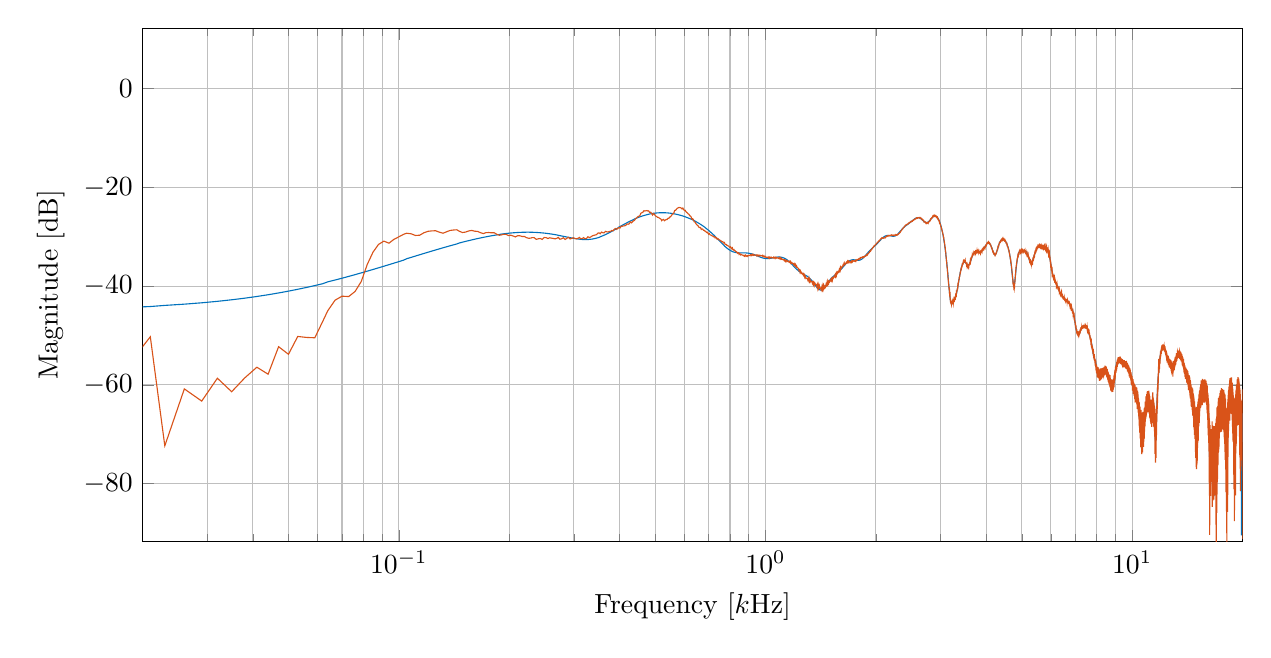
\begin{tikzpicture}

\begin{axis}[%
width=5.5in,
height=2.566in,
at={(1.281in,0.441in)},
scale only axis,
xmode=log,
xmin=0.020,
xmax=20.000,
xminorticks=true,
xlabel={Frequency [$k$Hz]},
xmajorgrids,
xminorgrids,
ymin=-91.672,
ymax=12.193,
ylabel={Magnitude [dB]},
ymajorgrids,
axis background/.style={fill=white},
title style={font=\bfseries},
legend style={legend cell align=left,align=left,draw=white!15!black}
]
\addplot [color=mycolor1,solid,forget plot]
  table[row sep=crcr]{%
0.018	-44.335\\
0.021	-44.134\\
0.023	-43.906\\
0.026	-43.653\\
0.029	-43.378\\
0.032	-43.082\\
0.035	-42.769\\
0.038	-42.441\\
0.041	-42.099\\
0.044	-41.746\\
0.047	-41.385\\
0.050	-41.017\\
0.053	-40.644\\
0.056	-40.269\\
0.059	-39.892\\
0.062	-39.516\\
0.064	-39.141\\
0.067	-38.769\\
0.070	-38.400\\
0.073	-38.036\\
0.076	-37.677\\
0.079	-37.323\\
0.082	-36.976\\
0.085	-36.636\\
0.088	-36.303\\
0.091	-35.977\\
0.094	-35.659\\
0.097	-35.348\\
0.100	-35.045\\
0.103	-34.751\\
0.105	-34.464\\
0.108	-34.185\\
0.111	-33.915\\
0.114	-33.652\\
0.117	-33.398\\
0.120	-33.151\\
0.123	-32.913\\
0.126	-32.683\\
0.129	-32.460\\
0.132	-32.245\\
0.135	-32.038\\
0.138	-31.839\\
0.141	-31.647\\
0.144	-31.463\\
0.146	-31.286\\
0.149	-31.117\\
0.152	-30.955\\
0.155	-30.800\\
0.158	-30.652\\
0.161	-30.512\\
0.164	-30.378\\
0.167	-30.252\\
0.170	-30.132\\
0.173	-30.020\\
0.176	-29.914\\
0.179	-29.814\\
0.182	-29.722\\
0.185	-29.636\\
0.188	-29.556\\
0.190	-29.483\\
0.193	-29.417\\
0.196	-29.356\\
0.199	-29.302\\
0.202	-29.255\\
0.205	-29.213\\
0.208	-29.177\\
0.211	-29.148\\
0.214	-29.124\\
0.217	-29.106\\
0.220	-29.094\\
0.223	-29.088\\
0.226	-29.088\\
0.229	-29.092\\
0.231	-29.103\\
0.234	-29.118\\
0.237	-29.139\\
0.240	-29.165\\
0.243	-29.195\\
0.246	-29.230\\
0.249	-29.270\\
0.252	-29.314\\
0.255	-29.362\\
0.258	-29.414\\
0.261	-29.469\\
0.264	-29.528\\
0.267	-29.589\\
0.270	-29.653\\
0.272	-29.718\\
0.275	-29.786\\
0.278	-29.854\\
0.281	-29.923\\
0.284	-29.992\\
0.287	-30.061\\
0.290	-30.128\\
0.293	-30.194\\
0.296	-30.256\\
0.299	-30.316\\
0.302	-30.371\\
0.305	-30.421\\
0.308	-30.466\\
0.311	-30.505\\
0.313	-30.536\\
0.316	-30.560\\
0.319	-30.576\\
0.322	-30.583\\
0.325	-30.580\\
0.328	-30.568\\
0.331	-30.546\\
0.334	-30.514\\
0.337	-30.472\\
0.340	-30.420\\
0.343	-30.359\\
0.346	-30.288\\
0.349	-30.208\\
0.352	-30.120\\
0.354	-30.023\\
0.357	-29.920\\
0.360	-29.810\\
0.363	-29.693\\
0.366	-29.572\\
0.369	-29.446\\
0.372	-29.316\\
0.375	-29.183\\
0.378	-29.048\\
0.381	-28.911\\
0.384	-28.772\\
0.387	-28.633\\
0.390	-28.494\\
0.393	-28.355\\
0.396	-28.216\\
0.398	-28.079\\
0.401	-27.943\\
0.404	-27.809\\
0.407	-27.678\\
0.410	-27.548\\
0.413	-27.421\\
0.416	-27.297\\
0.419	-27.176\\
0.422	-27.059\\
0.425	-26.944\\
0.428	-26.833\\
0.431	-26.725\\
0.434	-26.620\\
0.437	-26.520\\
0.439	-26.423\\
0.442	-26.329\\
0.445	-26.240\\
0.448	-26.154\\
0.451	-26.071\\
0.454	-25.993\\
0.457	-25.918\\
0.460	-25.847\\
0.463	-25.779\\
0.466	-25.716\\
0.469	-25.655\\
0.472	-25.599\\
0.475	-25.546\\
0.478	-25.496\\
0.480	-25.450\\
0.483	-25.408\\
0.486	-25.369\\
0.489	-25.333\\
0.492	-25.300\\
0.495	-25.271\\
0.498	-25.245\\
0.501	-25.222\\
0.504	-25.202\\
0.507	-25.185\\
0.510	-25.171\\
0.513	-25.160\\
0.516	-25.152\\
0.519	-25.146\\
0.521	-25.143\\
0.524	-25.143\\
0.527	-25.146\\
0.530	-25.151\\
0.533	-25.159\\
0.536	-25.169\\
0.539	-25.181\\
0.542	-25.196\\
0.545	-25.213\\
0.548	-25.233\\
0.551	-25.254\\
0.554	-25.278\\
0.557	-25.304\\
0.560	-25.332\\
0.563	-25.361\\
0.565	-25.393\\
0.568	-25.427\\
0.571	-25.462\\
0.574	-25.500\\
0.577	-25.539\\
0.580	-25.580\\
0.583	-25.622\\
0.586	-25.667\\
0.589	-25.713\\
0.592	-25.761\\
0.595	-25.810\\
0.598	-25.861\\
0.601	-25.914\\
0.604	-25.968\\
0.606	-26.024\\
0.609	-26.082\\
0.612	-26.141\\
0.615	-26.202\\
0.618	-26.264\\
0.621	-26.328\\
0.624	-26.394\\
0.627	-26.462\\
0.630	-26.531\\
0.633	-26.601\\
0.636	-26.674\\
0.639	-26.748\\
0.642	-26.824\\
0.645	-26.902\\
0.647	-26.981\\
0.650	-27.063\\
0.653	-27.146\\
0.656	-27.231\\
0.659	-27.318\\
0.662	-27.407\\
0.665	-27.498\\
0.668	-27.590\\
0.671	-27.685\\
0.674	-27.782\\
0.677	-27.881\\
0.680	-27.981\\
0.683	-28.084\\
0.686	-28.189\\
0.688	-28.296\\
0.691	-28.405\\
0.694	-28.515\\
0.697	-28.628\\
0.700	-28.743\\
0.703	-28.859\\
0.706	-28.978\\
0.709	-29.098\\
0.712	-29.219\\
0.715	-29.343\\
0.718	-29.468\\
0.721	-29.594\\
0.724	-29.721\\
0.727	-29.850\\
0.729	-29.980\\
0.732	-30.110\\
0.735	-30.241\\
0.738	-30.373\\
0.741	-30.505\\
0.744	-30.636\\
0.747	-30.768\\
0.750	-30.898\\
0.753	-31.028\\
0.756	-31.157\\
0.759	-31.284\\
0.762	-31.410\\
0.765	-31.534\\
0.768	-31.655\\
0.771	-31.773\\
0.773	-31.888\\
0.776	-32.000\\
0.779	-32.108\\
0.782	-32.212\\
0.785	-32.312\\
0.788	-32.407\\
0.791	-32.497\\
0.794	-32.582\\
0.797	-32.662\\
0.800	-32.737\\
0.803	-32.806\\
0.806	-32.870\\
0.809	-32.928\\
0.812	-32.981\\
0.814	-33.029\\
0.817	-33.071\\
0.820	-33.109\\
0.823	-33.142\\
0.826	-33.170\\
0.829	-33.194\\
0.832	-33.214\\
0.835	-33.230\\
0.838	-33.243\\
0.841	-33.254\\
0.844	-33.261\\
0.847	-33.267\\
0.850	-33.270\\
0.853	-33.273\\
0.855	-33.274\\
0.858	-33.274\\
0.861	-33.274\\
0.864	-33.273\\
0.867	-33.273\\
0.870	-33.273\\
0.873	-33.274\\
0.876	-33.275\\
0.879	-33.278\\
0.882	-33.282\\
0.885	-33.288\\
0.888	-33.295\\
0.891	-33.304\\
0.894	-33.315\\
0.896	-33.328\\
0.899	-33.343\\
0.902	-33.359\\
0.905	-33.378\\
0.908	-33.399\\
0.911	-33.422\\
0.914	-33.448\\
0.917	-33.475\\
0.920	-33.504\\
0.923	-33.535\\
0.926	-33.568\\
0.929	-33.602\\
0.932	-33.638\\
0.935	-33.675\\
0.938	-33.713\\
0.940	-33.753\\
0.943	-33.793\\
0.946	-33.834\\
0.949	-33.875\\
0.952	-33.916\\
0.955	-33.957\\
0.958	-33.998\\
0.961	-34.039\\
0.964	-34.078\\
0.967	-34.117\\
0.970	-34.154\\
0.973	-34.190\\
0.976	-34.224\\
0.979	-34.256\\
0.981	-34.286\\
0.984	-34.313\\
0.987	-34.338\\
0.990	-34.361\\
0.993	-34.380\\
0.996	-34.397\\
0.999	-34.411\\
1.002	-34.422\\
1.005	-34.430\\
1.008	-34.436\\
1.011	-34.438\\
1.014	-34.438\\
1.017	-34.435\\
1.020	-34.429\\
1.022	-34.421\\
1.025	-34.411\\
1.028	-34.399\\
1.031	-34.385\\
1.034	-34.370\\
1.037	-34.353\\
1.040	-34.335\\
1.043	-34.317\\
1.046	-34.298\\
1.049	-34.279\\
1.052	-34.259\\
1.055	-34.240\\
1.058	-34.221\\
1.061	-34.203\\
1.063	-34.186\\
1.066	-34.171\\
1.069	-34.156\\
1.072	-34.143\\
1.075	-34.132\\
1.078	-34.123\\
1.081	-34.116\\
1.084	-34.112\\
1.087	-34.110\\
1.090	-34.110\\
1.093	-34.114\\
1.096	-34.120\\
1.099	-34.129\\
1.102	-34.141\\
1.104	-34.156\\
1.107	-34.175\\
1.110	-34.196\\
1.113	-34.221\\
1.116	-34.249\\
1.119	-34.281\\
1.122	-34.316\\
1.125	-34.354\\
1.128	-34.395\\
1.131	-34.440\\
1.134	-34.487\\
1.137	-34.538\\
1.140	-34.592\\
1.143	-34.649\\
1.146	-34.709\\
1.148	-34.772\\
1.151	-34.837\\
1.154	-34.905\\
1.157	-34.975\\
1.160	-35.047\\
1.163	-35.122\\
1.166	-35.198\\
1.169	-35.277\\
1.172	-35.356\\
1.175	-35.437\\
1.178	-35.519\\
1.181	-35.602\\
1.184	-35.686\\
1.187	-35.770\\
1.189	-35.854\\
1.192	-35.938\\
1.195	-36.021\\
1.198	-36.104\\
1.201	-36.187\\
1.204	-36.268\\
1.207	-36.348\\
1.210	-36.426\\
1.213	-36.503\\
1.216	-36.578\\
1.219	-36.651\\
1.222	-36.722\\
1.225	-36.790\\
1.228	-36.857\\
1.230	-36.921\\
1.233	-36.982\\
1.236	-37.041\\
1.239	-37.098\\
1.242	-37.153\\
1.245	-37.205\\
1.248	-37.255\\
1.251	-37.304\\
1.254	-37.350\\
1.257	-37.395\\
1.260	-37.439\\
1.263	-37.482\\
1.266	-37.523\\
1.269	-37.564\\
1.271	-37.605\\
1.274	-37.645\\
1.277	-37.685\\
1.280	-37.726\\
1.283	-37.768\\
1.286	-37.810\\
1.289	-37.853\\
1.292	-37.898\\
1.295	-37.944\\
1.298	-37.992\\
1.301	-38.042\\
1.304	-38.095\\
1.307	-38.149\\
1.310	-38.206\\
1.313	-38.266\\
1.315	-38.328\\
1.318	-38.393\\
1.321	-38.461\\
1.324	-38.532\\
1.327	-38.605\\
1.330	-38.682\\
1.333	-38.761\\
1.336	-38.843\\
1.339	-38.928\\
1.342	-39.015\\
1.345	-39.104\\
1.348	-39.195\\
1.351	-39.288\\
1.354	-39.382\\
1.356	-39.478\\
1.359	-39.574\\
1.362	-39.670\\
1.365	-39.766\\
1.368	-39.862\\
1.371	-39.956\\
1.374	-40.048\\
1.377	-40.138\\
1.380	-40.224\\
1.383	-40.307\\
1.386	-40.385\\
1.389	-40.459\\
1.392	-40.526\\
1.395	-40.587\\
1.397	-40.640\\
1.400	-40.686\\
1.403	-40.725\\
1.406	-40.754\\
1.409	-40.775\\
1.412	-40.787\\
1.415	-40.790\\
1.418	-40.784\\
1.421	-40.768\\
1.424	-40.744\\
1.427	-40.712\\
1.430	-40.671\\
1.433	-40.623\\
1.436	-40.568\\
1.438	-40.506\\
1.441	-40.438\\
1.444	-40.366\\
1.447	-40.288\\
1.450	-40.206\\
1.453	-40.122\\
1.456	-40.034\\
1.459	-39.944\\
1.462	-39.853\\
1.465	-39.761\\
1.468	-39.669\\
1.471	-39.576\\
1.474	-39.484\\
1.477	-39.392\\
1.479	-39.302\\
1.482	-39.212\\
1.485	-39.125\\
1.488	-39.039\\
1.491	-38.955\\
1.494	-38.873\\
1.497	-38.794\\
1.500	-38.717\\
1.503	-38.642\\
1.506	-38.569\\
1.509	-38.499\\
1.512	-38.430\\
1.515	-38.364\\
1.518	-38.301\\
1.521	-38.239\\
1.523	-38.179\\
1.526	-38.121\\
1.529	-38.065\\
1.532	-38.010\\
1.535	-37.956\\
1.538	-37.904\\
1.541	-37.853\\
1.544	-37.802\\
1.547	-37.752\\
1.550	-37.703\\
1.553	-37.653\\
1.556	-37.604\\
1.559	-37.555\\
1.562	-37.505\\
1.564	-37.456\\
1.567	-37.405\\
1.570	-37.354\\
1.573	-37.302\\
1.576	-37.248\\
1.579	-37.194\\
1.582	-37.139\\
1.585	-37.083\\
1.588	-37.025\\
1.591	-36.966\\
1.594	-36.906\\
1.597	-36.845\\
1.600	-36.782\\
1.603	-36.718\\
1.605	-36.654\\
1.608	-36.588\\
1.611	-36.521\\
1.614	-36.454\\
1.617	-36.386\\
1.620	-36.317\\
1.623	-36.249\\
1.626	-36.180\\
1.629	-36.110\\
1.632	-36.042\\
1.635	-35.973\\
1.638	-35.905\\
1.641	-35.837\\
1.644	-35.770\\
1.646	-35.704\\
1.649	-35.640\\
1.652	-35.576\\
1.655	-35.514\\
1.658	-35.454\\
1.661	-35.395\\
1.664	-35.338\\
1.667	-35.283\\
1.670	-35.229\\
1.673	-35.178\\
1.676	-35.130\\
1.679	-35.083\\
1.682	-35.039\\
1.685	-34.997\\
1.688	-34.958\\
1.690	-34.921\\
1.693	-34.887\\
1.696	-34.856\\
1.699	-34.827\\
1.702	-34.800\\
1.705	-34.776\\
1.708	-34.755\\
1.711	-34.736\\
1.714	-34.720\\
1.717	-34.706\\
1.720	-34.694\\
1.723	-34.685\\
1.726	-34.678\\
1.729	-34.673\\
1.731	-34.670\\
1.734	-34.668\\
1.737	-34.669\\
1.740	-34.671\\
1.743	-34.674\\
1.746	-34.679\\
1.749	-34.685\\
1.752	-34.692\\
1.755	-34.700\\
1.758	-34.708\\
1.761	-34.716\\
1.764	-34.725\\
1.767	-34.733\\
1.770	-34.742\\
1.772	-34.749\\
1.775	-34.757\\
1.778	-34.763\\
1.781	-34.768\\
1.784	-34.772\\
1.787	-34.774\\
1.790	-34.774\\
1.793	-34.773\\
1.796	-34.769\\
1.799	-34.764\\
1.802	-34.756\\
1.805	-34.745\\
1.808	-34.732\\
1.811	-34.716\\
1.813	-34.698\\
1.816	-34.676\\
1.819	-34.652\\
1.822	-34.626\\
1.825	-34.596\\
1.828	-34.564\\
1.831	-34.529\\
1.834	-34.492\\
1.837	-34.452\\
1.840	-34.409\\
1.843	-34.365\\
1.846	-34.318\\
1.849	-34.270\\
1.852	-34.220\\
1.854	-34.168\\
1.857	-34.114\\
1.860	-34.060\\
1.863	-34.004\\
1.866	-33.947\\
1.869	-33.890\\
1.872	-33.832\\
1.875	-33.773\\
1.878	-33.715\\
1.881	-33.656\\
1.884	-33.597\\
1.887	-33.538\\
1.890	-33.479\\
1.893	-33.421\\
1.896	-33.363\\
1.898	-33.305\\
1.901	-33.248\\
1.904	-33.192\\
1.907	-33.137\\
1.910	-33.082\\
1.913	-33.028\\
1.916	-32.975\\
1.919	-32.922\\
1.922	-32.871\\
1.925	-32.820\\
1.928	-32.770\\
1.931	-32.721\\
1.934	-32.673\\
1.937	-32.625\\
1.939	-32.578\\
1.942	-32.532\\
1.945	-32.486\\
1.948	-32.441\\
1.951	-32.396\\
1.954	-32.352\\
1.957	-32.308\\
1.960	-32.265\\
1.963	-32.221\\
1.966	-32.178\\
1.969	-32.135\\
1.972	-32.092\\
1.975	-32.048\\
1.978	-32.005\\
1.980	-31.961\\
1.983	-31.918\\
1.986	-31.873\\
1.989	-31.829\\
1.992	-31.784\\
1.995	-31.739\\
1.998	-31.693\\
2.001	-31.647\\
2.004	-31.600\\
2.007	-31.553\\
2.010	-31.506\\
2.013	-31.458\\
2.016	-31.409\\
2.019	-31.360\\
2.021	-31.311\\
2.024	-31.261\\
2.027	-31.211\\
2.030	-31.160\\
2.033	-31.110\\
2.036	-31.059\\
2.039	-31.008\\
2.042	-30.957\\
2.045	-30.907\\
2.048	-30.856\\
2.051	-30.805\\
2.054	-30.755\\
2.057	-30.705\\
2.060	-30.656\\
2.063	-30.607\\
2.065	-30.559\\
2.068	-30.512\\
2.071	-30.465\\
2.074	-30.419\\
2.077	-30.375\\
2.080	-30.331\\
2.083	-30.289\\
2.086	-30.247\\
2.089	-30.207\\
2.092	-30.169\\
2.095	-30.132\\
2.098	-30.096\\
2.101	-30.062\\
2.104	-30.029\\
2.106	-29.998\\
2.109	-29.969\\
2.112	-29.941\\
2.115	-29.916\\
2.118	-29.892\\
2.121	-29.869\\
2.124	-29.849\\
2.127	-29.830\\
2.130	-29.814\\
2.133	-29.799\\
2.136	-29.785\\
2.139	-29.774\\
2.142	-29.764\\
2.145	-29.756\\
2.147	-29.750\\
2.150	-29.745\\
2.153	-29.742\\
2.156	-29.741\\
2.159	-29.741\\
2.162	-29.742\\
2.165	-29.745\\
2.168	-29.749\\
2.171	-29.754\\
2.174	-29.760\\
2.177	-29.767\\
2.180	-29.775\\
2.183	-29.784\\
2.186	-29.793\\
2.188	-29.803\\
2.191	-29.813\\
2.194	-29.823\\
2.197	-29.834\\
2.200	-29.844\\
2.203	-29.854\\
2.206	-29.864\\
2.209	-29.873\\
2.212	-29.882\\
2.215	-29.890\\
2.218	-29.897\\
2.221	-29.902\\
2.224	-29.907\\
2.227	-29.910\\
2.229	-29.912\\
2.232	-29.913\\
2.235	-29.911\\
2.238	-29.908\\
2.241	-29.903\\
2.244	-29.896\\
2.247	-29.887\\
2.250	-29.876\\
2.253	-29.863\\
2.256	-29.848\\
2.259	-29.831\\
2.262	-29.811\\
2.265	-29.789\\
2.268	-29.766\\
2.271	-29.740\\
2.273	-29.712\\
2.276	-29.682\\
2.279	-29.650\\
2.282	-29.616\\
2.285	-29.581\\
2.288	-29.544\\
2.291	-29.506\\
2.294	-29.466\\
2.297	-29.424\\
2.300	-29.382\\
2.303	-29.338\\
2.306	-29.293\\
2.309	-29.248\\
2.312	-29.202\\
2.314	-29.155\\
2.317	-29.108\\
2.320	-29.061\\
2.323	-29.013\\
2.326	-28.965\\
2.329	-28.917\\
2.332	-28.869\\
2.335	-28.821\\
2.338	-28.774\\
2.341	-28.727\\
2.344	-28.680\\
2.347	-28.634\\
2.350	-28.588\\
2.353	-28.543\\
2.355	-28.498\\
2.358	-28.455\\
2.361	-28.412\\
2.364	-28.369\\
2.367	-28.328\\
2.370	-28.287\\
2.373	-28.248\\
2.376	-28.209\\
2.379	-28.170\\
2.382	-28.133\\
2.385	-28.097\\
2.388	-28.061\\
2.391	-28.026\\
2.394	-27.992\\
2.396	-27.958\\
2.399	-27.926\\
2.402	-27.893\\
2.405	-27.862\\
2.408	-27.831\\
2.411	-27.801\\
2.414	-27.771\\
2.417	-27.742\\
2.420	-27.712\\
2.423	-27.684\\
2.426	-27.655\\
2.429	-27.627\\
2.432	-27.599\\
2.435	-27.572\\
2.438	-27.544\\
2.440	-27.516\\
2.443	-27.488\\
2.446	-27.461\\
2.449	-27.433\\
2.452	-27.405\\
2.455	-27.377\\
2.458	-27.349\\
2.461	-27.320\\
2.464	-27.291\\
2.467	-27.262\\
2.470	-27.233\\
2.473	-27.204\\
2.476	-27.174\\
2.479	-27.144\\
2.481	-27.113\\
2.484	-27.083\\
2.487	-27.052\\
2.490	-27.021\\
2.493	-26.989\\
2.496	-26.958\\
2.499	-26.926\\
2.502	-26.895\\
2.505	-26.863\\
2.508	-26.831\\
2.511	-26.799\\
2.514	-26.767\\
2.517	-26.736\\
2.520	-26.704\\
2.522	-26.673\\
2.525	-26.642\\
2.528	-26.612\\
2.531	-26.582\\
2.534	-26.552\\
2.537	-26.523\\
2.540	-26.495\\
2.543	-26.467\\
2.546	-26.440\\
2.549	-26.414\\
2.552	-26.389\\
2.555	-26.365\\
2.558	-26.341\\
2.561	-26.319\\
2.563	-26.298\\
2.566	-26.279\\
2.569	-26.260\\
2.572	-26.243\\
2.575	-26.227\\
2.578	-26.212\\
2.581	-26.199\\
2.584	-26.188\\
2.587	-26.178\\
2.590	-26.169\\
2.593	-26.162\\
2.596	-26.157\\
2.599	-26.153\\
2.602	-26.151\\
2.604	-26.150\\
2.607	-26.151\\
2.610	-26.154\\
2.613	-26.159\\
2.616	-26.165\\
2.619	-26.173\\
2.622	-26.182\\
2.625	-26.193\\
2.628	-26.206\\
2.631	-26.220\\
2.634	-26.236\\
2.637	-26.253\\
2.640	-26.272\\
2.643	-26.292\\
2.646	-26.314\\
2.648	-26.337\\
2.651	-26.361\\
2.654	-26.386\\
2.657	-26.413\\
2.660	-26.440\\
2.663	-26.468\\
2.666	-26.497\\
2.669	-26.527\\
2.672	-26.558\\
2.675	-26.589\\
2.678	-26.620\\
2.681	-26.652\\
2.684	-26.684\\
2.687	-26.716\\
2.689	-26.747\\
2.692	-26.779\\
2.695	-26.810\\
2.698	-26.840\\
2.701	-26.870\\
2.704	-26.899\\
2.707	-26.927\\
2.710	-26.954\\
2.713	-26.979\\
2.716	-27.003\\
2.719	-27.026\\
2.722	-27.047\\
2.725	-27.066\\
2.728	-27.083\\
2.730	-27.098\\
2.733	-27.111\\
2.736	-27.122\\
2.739	-27.131\\
2.742	-27.137\\
2.745	-27.141\\
2.748	-27.142\\
2.751	-27.141\\
2.754	-27.137\\
2.757	-27.130\\
2.760	-27.122\\
2.763	-27.110\\
2.766	-27.097\\
2.769	-27.080\\
2.771	-27.062\\
2.774	-27.041\\
2.777	-27.019\\
2.780	-26.994\\
2.783	-26.967\\
2.786	-26.938\\
2.789	-26.908\\
2.792	-26.876\\
2.795	-26.843\\
2.798	-26.808\\
2.801	-26.773\\
2.804	-26.736\\
2.807	-26.699\\
2.810	-26.660\\
2.813	-26.622\\
2.815	-26.583\\
2.818	-26.543\\
2.821	-26.504\\
2.824	-26.465\\
2.827	-26.426\\
2.830	-26.387\\
2.833	-26.349\\
2.836	-26.311\\
2.839	-26.274\\
2.842	-26.238\\
2.845	-26.203\\
2.848	-26.169\\
2.851	-26.136\\
2.854	-26.104\\
2.856	-26.074\\
2.859	-26.045\\
2.862	-26.018\\
2.865	-25.993\\
2.868	-25.969\\
2.871	-25.947\\
2.874	-25.927\\
2.877	-25.909\\
2.880	-25.893\\
2.883	-25.878\\
2.886	-25.866\\
2.889	-25.857\\
2.892	-25.849\\
2.895	-25.844\\
2.897	-25.841\\
2.900	-25.840\\
2.903	-25.842\\
2.906	-25.846\\
2.909	-25.853\\
2.912	-25.862\\
2.915	-25.874\\
2.918	-25.889\\
2.921	-25.906\\
2.924	-25.926\\
2.927	-25.948\\
2.930	-25.973\\
2.933	-26.001\\
2.936	-26.032\\
2.938	-26.066\\
2.941	-26.102\\
2.944	-26.141\\
2.947	-26.183\\
2.950	-26.228\\
2.953	-26.276\\
2.956	-26.327\\
2.959	-26.381\\
2.962	-26.438\\
2.965	-26.498\\
2.968	-26.561\\
2.971	-26.628\\
2.974	-26.697\\
2.977	-26.769\\
2.979	-26.845\\
2.982	-26.924\\
2.985	-27.006\\
2.988	-27.092\\
2.991	-27.181\\
2.994	-27.273\\
2.997	-27.369\\
3.000	-27.468\\
3.003	-27.571\\
3.006	-27.677\\
3.009	-27.786\\
3.012	-27.900\\
3.015	-28.017\\
3.018	-28.137\\
3.021	-28.262\\
3.023	-28.390\\
3.026	-28.522\\
3.029	-28.658\\
3.032	-28.798\\
3.035	-28.942\\
3.038	-29.090\\
3.041	-29.242\\
3.044	-29.399\\
3.047	-29.560\\
3.050	-29.725\\
3.053	-29.894\\
3.056	-30.068\\
3.059	-30.247\\
3.062	-30.430\\
3.064	-30.617\\
3.067	-30.810\\
3.070	-31.007\\
3.073	-31.210\\
3.076	-31.417\\
3.079	-31.630\\
3.082	-31.847\\
3.085	-32.070\\
3.088	-32.298\\
3.091	-32.532\\
3.094	-32.771\\
3.097	-33.016\\
3.100	-33.266\\
3.103	-33.522\\
3.105	-33.784\\
3.108	-34.051\\
3.111	-34.324\\
3.114	-34.603\\
3.117	-34.888\\
3.120	-35.178\\
3.123	-35.475\\
3.126	-35.776\\
3.129	-36.083\\
3.132	-36.396\\
3.135	-36.713\\
3.138	-37.035\\
3.141	-37.362\\
3.144	-37.692\\
3.146	-38.026\\
3.149	-38.362\\
3.152	-38.700\\
3.155	-39.039\\
3.158	-39.377\\
3.161	-39.714\\
3.164	-40.048\\
3.167	-40.378\\
3.170	-40.702\\
3.173	-41.017\\
3.176	-41.322\\
3.179	-41.614\\
3.182	-41.892\\
3.185	-42.154\\
3.188	-42.397\\
3.190	-42.619\\
3.193	-42.820\\
3.196	-42.998\\
3.199	-43.152\\
3.202	-43.282\\
3.205	-43.389\\
3.208	-43.472\\
3.211	-43.534\\
3.214	-43.576\\
3.217	-43.600\\
3.220	-43.607\\
3.223	-43.599\\
3.226	-43.579\\
3.229	-43.549\\
3.231	-43.510\\
3.234	-43.464\\
3.237	-43.413\\
3.240	-43.358\\
3.243	-43.300\\
3.246	-43.241\\
3.249	-43.180\\
3.252	-43.119\\
3.255	-43.059\\
3.258	-42.998\\
3.261	-42.938\\
3.264	-42.879\\
3.267	-42.820\\
3.270	-42.762\\
3.272	-42.703\\
3.275	-42.645\\
3.278	-42.585\\
3.281	-42.525\\
3.284	-42.463\\
3.287	-42.398\\
3.290	-42.331\\
3.293	-42.261\\
3.296	-42.187\\
3.299	-42.109\\
3.302	-42.026\\
3.305	-41.938\\
3.308	-41.845\\
3.311	-41.745\\
3.313	-41.640\\
3.316	-41.529\\
3.319	-41.411\\
3.322	-41.288\\
3.325	-41.158\\
3.328	-41.023\\
3.331	-40.882\\
3.334	-40.736\\
3.337	-40.586\\
3.340	-40.431\\
3.343	-40.272\\
3.346	-40.110\\
3.349	-39.945\\
3.352	-39.778\\
3.354	-39.609\\
3.357	-39.439\\
3.360	-39.269\\
3.363	-39.098\\
3.366	-38.928\\
3.369	-38.759\\
3.372	-38.591\\
3.375	-38.425\\
3.378	-38.260\\
3.381	-38.099\\
3.384	-37.940\\
3.387	-37.784\\
3.390	-37.631\\
3.393	-37.482\\
3.396	-37.337\\
3.398	-37.196\\
3.401	-37.059\\
3.404	-36.926\\
3.407	-36.798\\
3.410	-36.674\\
3.413	-36.555\\
3.416	-36.441\\
3.419	-36.332\\
3.422	-36.227\\
3.425	-36.127\\
3.428	-36.032\\
3.431	-35.943\\
3.434	-35.858\\
3.437	-35.778\\
3.439	-35.703\\
3.442	-35.633\\
3.445	-35.568\\
3.448	-35.509\\
3.451	-35.453\\
3.454	-35.403\\
3.457	-35.358\\
3.460	-35.317\\
3.463	-35.281\\
3.466	-35.250\\
3.469	-35.223\\
3.472	-35.200\\
3.475	-35.182\\
3.478	-35.168\\
3.480	-35.159\\
3.483	-35.153\\
3.486	-35.151\\
3.489	-35.153\\
3.492	-35.158\\
3.495	-35.167\\
3.498	-35.179\\
3.501	-35.194\\
3.504	-35.212\\
3.507	-35.232\\
3.510	-35.255\\
3.513	-35.280\\
3.516	-35.306\\
3.519	-35.334\\
3.521	-35.364\\
3.524	-35.394\\
3.527	-35.425\\
3.530	-35.456\\
3.533	-35.488\\
3.536	-35.519\\
3.539	-35.549\\
3.542	-35.578\\
3.545	-35.605\\
3.548	-35.631\\
3.551	-35.655\\
3.554	-35.676\\
3.557	-35.694\\
3.560	-35.709\\
3.563	-35.720\\
3.565	-35.728\\
3.568	-35.731\\
3.571	-35.731\\
3.574	-35.726\\
3.577	-35.716\\
3.580	-35.702\\
3.583	-35.683\\
3.586	-35.659\\
3.589	-35.631\\
3.592	-35.598\\
3.595	-35.561\\
3.598	-35.519\\
3.601	-35.473\\
3.604	-35.423\\
3.606	-35.369\\
3.609	-35.312\\
3.612	-35.252\\
3.615	-35.188\\
3.618	-35.122\\
3.621	-35.054\\
3.624	-34.984\\
3.627	-34.912\\
3.630	-34.839\\
3.633	-34.765\\
3.636	-34.691\\
3.639	-34.615\\
3.642	-34.540\\
3.645	-34.465\\
3.647	-34.391\\
3.650	-34.317\\
3.653	-34.244\\
3.656	-34.172\\
3.659	-34.101\\
3.662	-34.032\\
3.665	-33.964\\
3.668	-33.898\\
3.671	-33.835\\
3.674	-33.773\\
3.677	-33.713\\
3.680	-33.656\\
3.683	-33.601\\
3.686	-33.548\\
3.688	-33.498\\
3.691	-33.450\\
3.694	-33.405\\
3.697	-33.362\\
3.700	-33.322\\
3.703	-33.284\\
3.706	-33.249\\
3.709	-33.217\\
3.712	-33.187\\
3.715	-33.159\\
3.718	-33.134\\
3.721	-33.112\\
3.724	-33.091\\
3.727	-33.073\\
3.729	-33.058\\
3.732	-33.044\\
3.735	-33.033\\
3.738	-33.023\\
3.741	-33.016\\
3.744	-33.010\\
3.747	-33.007\\
3.750	-33.004\\
3.753	-33.004\\
3.756	-33.005\\
3.759	-33.007\\
3.762	-33.010\\
3.765	-33.015\\
3.768	-33.021\\
3.771	-33.027\\
3.773	-33.034\\
3.776	-33.042\\
3.779	-33.051\\
3.782	-33.060\\
3.785	-33.069\\
3.788	-33.078\\
3.791	-33.088\\
3.794	-33.097\\
3.797	-33.106\\
3.800	-33.115\\
3.803	-33.124\\
3.806	-33.132\\
3.809	-33.139\\
3.812	-33.146\\
3.814	-33.152\\
3.817	-33.158\\
3.820	-33.162\\
3.823	-33.165\\
3.826	-33.168\\
3.829	-33.169\\
3.832	-33.169\\
3.835	-33.168\\
3.838	-33.165\\
3.841	-33.161\\
3.844	-33.156\\
3.847	-33.150\\
3.850	-33.142\\
3.853	-33.133\\
3.855	-33.123\\
3.858	-33.111\\
3.861	-33.098\\
3.864	-33.083\\
3.867	-33.068\\
3.870	-33.051\\
3.873	-33.032\\
3.876	-33.013\\
3.879	-32.992\\
3.882	-32.970\\
3.885	-32.947\\
3.888	-32.923\\
3.891	-32.898\\
3.894	-32.872\\
3.896	-32.845\\
3.899	-32.817\\
3.902	-32.788\\
3.905	-32.758\\
3.908	-32.727\\
3.911	-32.696\\
3.914	-32.664\\
3.917	-32.631\\
3.920	-32.598\\
3.923	-32.564\\
3.926	-32.529\\
3.929	-32.494\\
3.932	-32.459\\
3.935	-32.423\\
3.938	-32.387\\
3.940	-32.350\\
3.943	-32.314\\
3.946	-32.277\\
3.949	-32.239\\
3.952	-32.202\\
3.955	-32.165\\
3.958	-32.128\\
3.961	-32.090\\
3.964	-32.053\\
3.967	-32.016\\
3.970	-31.979\\
3.973	-31.943\\
3.976	-31.906\\
3.979	-31.870\\
3.981	-31.835\\
3.984	-31.800\\
3.987	-31.766\\
3.990	-31.732\\
3.993	-31.699\\
3.996	-31.667\\
3.999	-31.636\\
4.002	-31.605\\
4.005	-31.576\\
4.008	-31.547\\
4.011	-31.520\\
4.014	-31.494\\
4.017	-31.469\\
4.020	-31.445\\
4.022	-31.423\\
4.025	-31.402\\
4.028	-31.383\\
4.031	-31.365\\
4.034	-31.349\\
4.037	-31.335\\
4.040	-31.322\\
4.043	-31.312\\
4.046	-31.303\\
4.049	-31.296\\
4.052	-31.291\\
4.055	-31.289\\
4.058	-31.288\\
4.061	-31.289\\
4.063	-31.293\\
4.066	-31.299\\
4.069	-31.307\\
4.072	-31.318\\
4.075	-31.331\\
4.078	-31.346\\
4.081	-31.364\\
4.084	-31.384\\
4.087	-31.407\\
4.090	-31.432\\
4.093	-31.460\\
4.096	-31.490\\
4.099	-31.523\\
4.102	-31.558\\
4.104	-31.595\\
4.107	-31.635\\
4.110	-31.677\\
4.113	-31.722\\
4.116	-31.769\\
4.119	-31.818\\
4.122	-31.870\\
4.125	-31.923\\
4.128	-31.979\\
4.131	-32.036\\
4.134	-32.096\\
4.137	-32.157\\
4.140	-32.219\\
4.143	-32.283\\
4.146	-32.349\\
4.148	-32.415\\
4.151	-32.483\\
4.154	-32.551\\
4.157	-32.619\\
4.160	-32.688\\
4.163	-32.757\\
4.166	-32.826\\
4.169	-32.894\\
4.172	-32.962\\
4.175	-33.028\\
4.178	-33.093\\
4.181	-33.156\\
4.184	-33.217\\
4.187	-33.276\\
4.189	-33.332\\
4.192	-33.385\\
4.195	-33.435\\
4.198	-33.481\\
4.201	-33.523\\
4.204	-33.561\\
4.207	-33.595\\
4.210	-33.623\\
4.213	-33.647\\
4.216	-33.665\\
4.219	-33.679\\
4.222	-33.686\\
4.225	-33.688\\
4.228	-33.685\\
4.230	-33.676\\
4.233	-33.662\\
4.236	-33.642\\
4.239	-33.617\\
4.242	-33.587\\
4.245	-33.552\\
4.248	-33.512\\
4.251	-33.467\\
4.254	-33.419\\
4.257	-33.366\\
4.260	-33.310\\
4.263	-33.250\\
4.266	-33.187\\
4.269	-33.122\\
4.271	-33.054\\
4.274	-32.984\\
4.277	-32.912\\
4.280	-32.839\\
4.283	-32.764\\
4.286	-32.689\\
4.289	-32.613\\
4.292	-32.537\\
4.295	-32.460\\
4.298	-32.383\\
4.301	-32.307\\
4.304	-32.231\\
4.307	-32.156\\
4.310	-32.082\\
4.313	-32.009\\
4.315	-31.937\\
4.318	-31.866\\
4.321	-31.796\\
4.324	-31.728\\
4.327	-31.662\\
4.330	-31.597\\
4.333	-31.534\\
4.336	-31.473\\
4.339	-31.414\\
4.342	-31.356\\
4.345	-31.301\\
4.348	-31.247\\
4.351	-31.195\\
4.354	-31.146\\
4.356	-31.098\\
4.359	-31.053\\
4.362	-31.009\\
4.365	-30.967\\
4.368	-30.928\\
4.371	-30.890\\
4.374	-30.855\\
4.377	-30.821\\
4.380	-30.790\\
4.383	-30.760\\
4.386	-30.732\\
4.389	-30.707\\
4.392	-30.683\\
4.395	-30.660\\
4.397	-30.640\\
4.400	-30.622\\
4.403	-30.605\\
4.406	-30.589\\
4.409	-30.576\\
4.412	-30.564\\
4.415	-30.554\\
4.418	-30.545\\
4.421	-30.538\\
4.424	-30.532\\
4.427	-30.528\\
4.430	-30.525\\
4.433	-30.524\\
4.436	-30.523\\
4.438	-30.525\\
4.441	-30.527\\
4.444	-30.531\\
4.447	-30.536\\
4.450	-30.542\\
4.453	-30.550\\
4.456	-30.559\\
4.459	-30.568\\
4.462	-30.579\\
4.465	-30.591\\
4.468	-30.604\\
4.471	-30.619\\
4.474	-30.634\\
4.477	-30.650\\
4.479	-30.668\\
4.482	-30.686\\
4.485	-30.706\\
4.488	-30.726\\
4.491	-30.748\\
4.494	-30.770\\
4.497	-30.794\\
4.500	-30.819\\
4.503	-30.844\\
4.506	-30.871\\
4.509	-30.899\\
4.512	-30.928\\
4.515	-30.959\\
4.518	-30.990\\
4.521	-31.022\\
4.523	-31.056\\
4.526	-31.091\\
4.529	-31.127\\
4.532	-31.164\\
4.535	-31.203\\
4.538	-31.243\\
4.541	-31.284\\
4.544	-31.327\\
4.547	-31.372\\
4.550	-31.417\\
4.553	-31.465\\
4.556	-31.513\\
4.559	-31.564\\
4.562	-31.616\\
4.564	-31.670\\
4.567	-31.725\\
4.570	-31.783\\
4.573	-31.842\\
4.576	-31.903\\
4.579	-31.967\\
4.582	-32.032\\
4.585	-32.099\\
4.588	-32.169\\
4.591	-32.241\\
4.594	-32.315\\
4.597	-32.391\\
4.600	-32.470\\
4.603	-32.551\\
4.605	-32.635\\
4.608	-32.722\\
4.611	-32.811\\
4.614	-32.904\\
4.617	-32.999\\
4.620	-33.097\\
4.623	-33.198\\
4.626	-33.302\\
4.629	-33.409\\
4.632	-33.520\\
4.635	-33.633\\
4.638	-33.751\\
4.641	-33.871\\
4.644	-33.996\\
4.646	-34.123\\
4.649	-34.255\\
4.652	-34.390\\
4.655	-34.529\\
4.658	-34.672\\
4.661	-34.819\\
4.664	-34.969\\
4.667	-35.124\\
4.670	-35.282\\
4.673	-35.445\\
4.676	-35.611\\
4.679	-35.781\\
4.682	-35.954\\
4.685	-36.131\\
4.688	-36.312\\
4.690	-36.495\\
4.693	-36.682\\
4.696	-36.871\\
4.699	-37.062\\
4.702	-37.255\\
4.705	-37.449\\
4.708	-37.644\\
4.711	-37.838\\
4.714	-38.031\\
4.717	-38.221\\
4.720	-38.409\\
4.723	-38.592\\
4.726	-38.769\\
4.729	-38.938\\
4.731	-39.098\\
4.734	-39.248\\
4.737	-39.385\\
4.740	-39.508\\
4.743	-39.615\\
4.746	-39.705\\
4.749	-39.775\\
4.752	-39.826\\
4.755	-39.856\\
4.758	-39.865\\
4.761	-39.852\\
4.764	-39.818\\
4.767	-39.763\\
4.770	-39.688\\
4.772	-39.595\\
4.775	-39.484\\
4.778	-39.358\\
4.781	-39.218\\
4.784	-39.066\\
4.787	-38.903\\
4.790	-38.732\\
4.793	-38.553\\
4.796	-38.369\\
4.799	-38.181\\
4.802	-37.990\\
4.805	-37.798\\
4.808	-37.604\\
4.811	-37.412\\
4.813	-37.220\\
4.816	-37.030\\
4.819	-36.843\\
4.822	-36.658\\
4.825	-36.477\\
4.828	-36.299\\
4.831	-36.125\\
4.834	-35.956\\
4.837	-35.791\\
4.840	-35.631\\
4.843	-35.475\\
4.846	-35.324\\
4.849	-35.178\\
4.852	-35.037\\
4.854	-34.901\\
4.857	-34.770\\
4.860	-34.644\\
4.863	-34.522\\
4.866	-34.406\\
4.869	-34.294\\
4.872	-34.187\\
4.875	-34.085\\
4.878	-33.988\\
4.881	-33.895\\
4.884	-33.807\\
4.887	-33.723\\
4.890	-33.644\\
4.893	-33.569\\
4.896	-33.498\\
4.898	-33.432\\
4.901	-33.369\\
4.904	-33.311\\
4.907	-33.256\\
4.910	-33.205\\
4.913	-33.158\\
4.916	-33.115\\
4.919	-33.075\\
4.922	-33.038\\
4.925	-33.005\\
4.928	-32.975\\
4.931	-32.948\\
4.934	-32.924\\
4.937	-32.903\\
4.939	-32.884\\
4.942	-32.869\\
4.945	-32.855\\
4.948	-32.844\\
4.951	-32.836\\
4.954	-32.829\\
4.957	-32.825\\
4.960	-32.822\\
4.963	-32.821\\
4.966	-32.821\\
4.969	-32.824\\
4.972	-32.827\\
4.975	-32.831\\
4.978	-32.837\\
4.980	-32.843\\
4.983	-32.851\\
4.986	-32.859\\
4.989	-32.867\\
4.992	-32.876\\
4.995	-32.885\\
4.998	-32.894\\
5.001	-32.903\\
5.004	-32.912\\
5.007	-32.921\\
5.010	-32.929\\
5.013	-32.938\\
5.016	-32.945\\
5.019	-32.952\\
5.021	-32.959\\
5.024	-32.965\\
5.027	-32.970\\
5.030	-32.974\\
5.033	-32.978\\
5.036	-32.981\\
5.039	-32.983\\
5.042	-32.984\\
5.045	-32.985\\
5.048	-32.984\\
5.051	-32.983\\
5.054	-32.982\\
5.057	-32.979\\
5.060	-32.977\\
5.063	-32.973\\
5.065	-32.970\\
5.068	-32.965\\
5.071	-32.961\\
5.074	-32.957\\
5.077	-32.952\\
5.080	-32.948\\
5.083	-32.943\\
5.086	-32.939\\
5.089	-32.936\\
5.092	-32.932\\
5.095	-32.930\\
5.098	-32.928\\
5.101	-32.926\\
5.104	-32.926\\
5.106	-32.927\\
5.109	-32.928\\
5.112	-32.931\\
5.115	-32.935\\
5.118	-32.941\\
5.121	-32.948\\
5.124	-32.956\\
5.127	-32.966\\
5.130	-32.978\\
5.133	-32.991\\
5.136	-33.007\\
5.139	-33.024\\
5.142	-33.042\\
5.145	-33.063\\
5.147	-33.086\\
5.150	-33.111\\
5.153	-33.138\\
5.156	-33.167\\
5.159	-33.197\\
5.162	-33.230\\
5.165	-33.265\\
5.168	-33.302\\
5.171	-33.341\\
5.174	-33.382\\
5.177	-33.425\\
5.180	-33.470\\
5.183	-33.517\\
5.186	-33.565\\
5.188	-33.615\\
5.191	-33.667\\
5.194	-33.721\\
5.197	-33.776\\
5.200	-33.832\\
5.203	-33.889\\
5.206	-33.948\\
5.209	-34.008\\
5.212	-34.068\\
5.215	-34.129\\
5.218	-34.191\\
5.221	-34.253\\
5.224	-34.316\\
5.227	-34.378\\
5.229	-34.440\\
5.232	-34.502\\
5.235	-34.564\\
5.238	-34.624\\
5.241	-34.684\\
5.244	-34.742\\
5.247	-34.799\\
5.250	-34.854\\
5.253	-34.907\\
5.256	-34.959\\
5.259	-35.008\\
5.262	-35.054\\
5.265	-35.098\\
5.268	-35.139\\
5.271	-35.176\\
5.273	-35.211\\
5.276	-35.242\\
5.279	-35.270\\
5.282	-35.293\\
5.285	-35.314\\
5.288	-35.330\\
5.291	-35.343\\
5.294	-35.351\\
5.297	-35.356\\
5.300	-35.357\\
5.303	-35.354\\
5.306	-35.347\\
5.309	-35.337\\
5.312	-35.323\\
5.314	-35.305\\
5.317	-35.284\\
5.320	-35.259\\
5.323	-35.232\\
5.326	-35.201\\
5.329	-35.168\\
5.332	-35.132\\
5.335	-35.093\\
5.338	-35.052\\
5.341	-35.009\\
5.344	-34.964\\
5.347	-34.917\\
5.350	-34.868\\
5.353	-34.818\\
5.355	-34.767\\
5.358	-34.714\\
5.361	-34.661\\
5.364	-34.606\\
5.367	-34.551\\
5.370	-34.495\\
5.373	-34.438\\
5.376	-34.381\\
5.379	-34.324\\
5.382	-34.267\\
5.385	-34.209\\
5.388	-34.152\\
5.391	-34.094\\
5.394	-34.037\\
5.396	-33.979\\
5.399	-33.922\\
5.402	-33.865\\
5.405	-33.809\\
5.408	-33.753\\
5.411	-33.697\\
5.414	-33.642\\
5.417	-33.587\\
5.420	-33.533\\
5.423	-33.479\\
5.426	-33.426\\
5.429	-33.374\\
5.432	-33.322\\
5.435	-33.270\\
5.438	-33.219\\
5.440	-33.169\\
5.443	-33.120\\
5.446	-33.071\\
5.449	-33.023\\
5.452	-32.976\\
5.455	-32.929\\
5.458	-32.883\\
5.461	-32.838\\
5.464	-32.793\\
5.467	-32.750\\
5.470	-32.707\\
5.473	-32.665\\
5.476	-32.623\\
5.479	-32.583\\
5.481	-32.543\\
5.484	-32.505\\
5.487	-32.467\\
5.490	-32.430\\
5.493	-32.394\\
5.496	-32.359\\
5.499	-32.324\\
5.502	-32.291\\
5.505	-32.259\\
5.508	-32.228\\
5.511	-32.197\\
5.514	-32.168\\
5.517	-32.140\\
5.520	-32.113\\
5.522	-32.087\\
5.525	-32.062\\
5.528	-32.038\\
5.531	-32.015\\
5.534	-31.994\\
5.537	-31.973\\
5.540	-31.954\\
5.543	-31.936\\
5.546	-31.919\\
5.549	-31.903\\
5.552	-31.888\\
5.555	-31.874\\
5.558	-31.862\\
5.561	-31.851\\
5.563	-31.841\\
5.566	-31.832\\
5.569	-31.824\\
5.572	-31.818\\
5.575	-31.812\\
5.578	-31.808\\
5.581	-31.804\\
5.584	-31.802\\
5.587	-31.801\\
5.590	-31.801\\
5.593	-31.802\\
5.596	-31.804\\
5.599	-31.806\\
5.602	-31.810\\
5.604	-31.815\\
5.607	-31.820\\
5.610	-31.826\\
5.613	-31.833\\
5.616	-31.841\\
5.619	-31.849\\
5.622	-31.858\\
5.625	-31.868\\
5.628	-31.878\\
5.631	-31.889\\
5.634	-31.900\\
5.637	-31.911\\
5.640	-31.923\\
5.643	-31.935\\
5.646	-31.947\\
5.648	-31.959\\
5.651	-31.972\\
5.654	-31.984\\
5.657	-31.997\\
5.660	-32.009\\
5.663	-32.021\\
5.666	-32.033\\
5.669	-32.045\\
5.672	-32.057\\
5.675	-32.068\\
5.678	-32.079\\
5.681	-32.089\\
5.684	-32.099\\
5.687	-32.109\\
5.689	-32.118\\
5.692	-32.126\\
5.695	-32.134\\
5.698	-32.141\\
5.701	-32.148\\
5.704	-32.154\\
5.707	-32.159\\
5.710	-32.164\\
5.713	-32.168\\
5.716	-32.171\\
5.719	-32.174\\
5.722	-32.176\\
5.725	-32.177\\
5.728	-32.178\\
5.730	-32.178\\
5.733	-32.178\\
5.736	-32.177\\
5.739	-32.176\\
5.742	-32.174\\
5.745	-32.172\\
5.748	-32.170\\
5.751	-32.167\\
5.754	-32.164\\
5.757	-32.161\\
5.760	-32.157\\
5.763	-32.154\\
5.766	-32.150\\
5.769	-32.147\\
5.771	-32.144\\
5.774	-32.140\\
5.777	-32.138\\
5.780	-32.135\\
5.783	-32.133\\
5.786	-32.131\\
5.789	-32.129\\
5.792	-32.129\\
5.795	-32.128\\
5.798	-32.129\\
5.801	-32.130\\
5.804	-32.132\\
5.807	-32.135\\
5.810	-32.139\\
5.813	-32.143\\
5.815	-32.149\\
5.818	-32.156\\
5.821	-32.164\\
5.824	-32.173\\
5.827	-32.183\\
5.830	-32.194\\
5.833	-32.207\\
5.836	-32.221\\
5.839	-32.237\\
5.842	-32.254\\
5.845	-32.272\\
5.848	-32.292\\
5.851	-32.313\\
5.854	-32.336\\
5.856	-32.360\\
5.859	-32.386\\
5.862	-32.414\\
5.865	-32.443\\
5.868	-32.474\\
5.871	-32.507\\
5.874	-32.541\\
5.877	-32.577\\
5.880	-32.615\\
5.883	-32.654\\
5.886	-32.696\\
5.889	-32.739\\
5.892	-32.783\\
5.895	-32.830\\
5.897	-32.878\\
5.900	-32.928\\
5.903	-32.979\\
5.906	-33.033\\
5.909	-33.088\\
5.912	-33.144\\
5.915	-33.203\\
5.918	-33.263\\
5.921	-33.325\\
5.924	-33.388\\
5.927	-33.453\\
5.930	-33.520\\
5.933	-33.588\\
5.936	-33.658\\
5.938	-33.729\\
5.941	-33.802\\
5.944	-33.876\\
5.947	-33.952\\
5.950	-34.029\\
5.953	-34.107\\
5.956	-34.187\\
5.959	-34.268\\
5.962	-34.350\\
5.965	-34.433\\
5.968	-34.518\\
5.971	-34.603\\
5.974	-34.689\\
5.977	-34.777\\
5.979	-34.865\\
5.982	-34.954\\
5.985	-35.043\\
5.988	-35.133\\
5.991	-35.224\\
5.994	-35.315\\
5.997	-35.407\\
6.000	-35.499\\
6.003	-35.591\\
6.006	-35.684\\
6.009	-35.776\\
6.012	-35.868\\
6.015	-35.961\\
6.018	-36.053\\
6.021	-36.145\\
6.023	-36.236\\
6.026	-36.327\\
6.029	-36.418\\
6.032	-36.507\\
6.035	-36.597\\
6.038	-36.685\\
6.041	-36.772\\
6.044	-36.859\\
6.047	-36.944\\
6.050	-37.028\\
6.053	-37.111\\
6.056	-37.192\\
6.059	-37.273\\
6.062	-37.351\\
6.064	-37.429\\
6.067	-37.504\\
6.070	-37.578\\
6.073	-37.651\\
6.076	-37.722\\
6.079	-37.791\\
6.082	-37.858\\
6.085	-37.923\\
6.088	-37.987\\
6.091	-38.049\\
6.094	-38.109\\
6.097	-38.167\\
6.100	-38.223\\
6.103	-38.278\\
6.105	-38.331\\
6.108	-38.382\\
6.111	-38.431\\
6.114	-38.479\\
6.117	-38.525\\
6.120	-38.569\\
6.123	-38.612\\
6.126	-38.654\\
6.129	-38.694\\
6.132	-38.732\\
6.135	-38.770\\
6.138	-38.806\\
6.141	-38.841\\
6.144	-38.874\\
6.146	-38.907\\
6.149	-38.939\\
6.152	-38.970\\
6.155	-39.000\\
6.158	-39.029\\
6.161	-39.058\\
6.164	-39.086\\
6.167	-39.114\\
6.170	-39.141\\
6.173	-39.168\\
6.176	-39.194\\
6.179	-39.220\\
6.182	-39.246\\
6.185	-39.272\\
6.188	-39.298\\
6.190	-39.324\\
6.193	-39.350\\
6.196	-39.376\\
6.199	-39.402\\
6.202	-39.429\\
6.205	-39.456\\
6.208	-39.483\\
6.211	-39.510\\
6.214	-39.538\\
6.217	-39.566\\
6.220	-39.595\\
6.223	-39.624\\
6.226	-39.654\\
6.229	-39.684\\
6.231	-39.715\\
6.234	-39.747\\
6.237	-39.779\\
6.240	-39.811\\
6.243	-39.845\\
6.246	-39.879\\
6.249	-39.913\\
6.252	-39.949\\
6.255	-39.984\\
6.258	-40.021\\
6.261	-40.058\\
6.264	-40.096\\
6.267	-40.134\\
6.270	-40.173\\
6.272	-40.212\\
6.275	-40.252\\
6.278	-40.292\\
6.281	-40.333\\
6.284	-40.374\\
6.287	-40.415\\
6.290	-40.457\\
6.293	-40.499\\
6.296	-40.541\\
6.299	-40.584\\
6.302	-40.626\\
6.305	-40.669\\
6.308	-40.712\\
6.311	-40.754\\
6.313	-40.796\\
6.316	-40.839\\
6.319	-40.881\\
6.322	-40.923\\
6.325	-40.964\\
6.328	-41.005\\
6.331	-41.045\\
6.334	-41.085\\
6.337	-41.125\\
6.340	-41.163\\
6.343	-41.201\\
6.346	-41.239\\
6.349	-41.275\\
6.352	-41.311\\
6.354	-41.346\\
6.357	-41.380\\
6.360	-41.413\\
6.363	-41.445\\
6.366	-41.476\\
6.369	-41.506\\
6.372	-41.535\\
6.375	-41.563\\
6.378	-41.590\\
6.381	-41.616\\
6.384	-41.641\\
6.387	-41.665\\
6.390	-41.688\\
6.393	-41.710\\
6.396	-41.731\\
6.398	-41.752\\
6.401	-41.771\\
6.404	-41.790\\
6.407	-41.808\\
6.410	-41.826\\
6.413	-41.843\\
6.416	-41.859\\
6.419	-41.875\\
6.422	-41.891\\
6.425	-41.906\\
6.428	-41.921\\
6.431	-41.935\\
6.434	-41.950\\
6.437	-41.964\\
6.439	-41.979\\
6.442	-41.993\\
6.445	-42.007\\
6.448	-42.022\\
6.451	-42.037\\
6.454	-42.052\\
6.457	-42.067\\
6.460	-42.082\\
6.463	-42.098\\
6.466	-42.115\\
6.469	-42.131\\
6.472	-42.148\\
6.475	-42.166\\
6.478	-42.184\\
6.480	-42.202\\
6.483	-42.221\\
6.486	-42.241\\
6.489	-42.261\\
6.492	-42.281\\
6.495	-42.302\\
6.498	-42.323\\
6.501	-42.345\\
6.504	-42.367\\
6.507	-42.389\\
6.510	-42.412\\
6.513	-42.434\\
6.516	-42.457\\
6.519	-42.481\\
6.521	-42.504\\
6.524	-42.527\\
6.527	-42.550\\
6.530	-42.573\\
6.533	-42.596\\
6.536	-42.619\\
6.539	-42.641\\
6.542	-42.663\\
6.545	-42.685\\
6.548	-42.706\\
6.551	-42.727\\
6.554	-42.747\\
6.557	-42.766\\
6.560	-42.785\\
6.563	-42.803\\
6.565	-42.820\\
6.568	-42.837\\
6.571	-42.852\\
6.574	-42.867\\
6.577	-42.881\\
6.580	-42.893\\
6.583	-42.905\\
6.586	-42.916\\
6.589	-42.926\\
6.592	-42.936\\
6.595	-42.944\\
6.598	-42.951\\
6.601	-42.958\\
6.604	-42.964\\
6.606	-42.969\\
6.609	-42.974\\
6.612	-42.978\\
6.615	-42.981\\
6.618	-42.984\\
6.621	-42.987\\
6.624	-42.989\\
6.627	-42.991\\
6.630	-42.993\\
6.633	-42.995\\
6.636	-42.997\\
6.639	-42.998\\
6.642	-43.000\\
6.645	-43.003\\
6.647	-43.005\\
6.650	-43.008\\
6.653	-43.011\\
6.656	-43.015\\
6.659	-43.020\\
6.662	-43.025\\
6.665	-43.031\\
6.668	-43.038\\
6.671	-43.046\\
6.674	-43.054\\
6.677	-43.064\\
6.680	-43.074\\
6.683	-43.086\\
6.686	-43.098\\
6.688	-43.112\\
6.691	-43.127\\
6.694	-43.143\\
6.697	-43.160\\
6.700	-43.178\\
6.703	-43.197\\
6.706	-43.218\\
6.709	-43.239\\
6.712	-43.262\\
6.715	-43.285\\
6.718	-43.310\\
6.721	-43.335\\
6.724	-43.362\\
6.727	-43.389\\
6.729	-43.417\\
6.732	-43.446\\
6.735	-43.476\\
6.738	-43.507\\
6.741	-43.538\\
6.744	-43.569\\
6.747	-43.601\\
6.750	-43.633\\
6.753	-43.666\\
6.756	-43.699\\
6.759	-43.732\\
6.762	-43.765\\
6.765	-43.799\\
6.768	-43.832\\
6.771	-43.865\\
6.773	-43.898\\
6.776	-43.930\\
6.779	-43.963\\
6.782	-43.995\\
6.785	-44.027\\
6.788	-44.058\\
6.791	-44.089\\
6.794	-44.119\\
6.797	-44.149\\
6.800	-44.178\\
6.803	-44.207\\
6.806	-44.235\\
6.809	-44.263\\
6.812	-44.291\\
6.814	-44.318\\
6.817	-44.344\\
6.820	-44.370\\
6.823	-44.396\\
6.826	-44.422\\
6.829	-44.448\\
6.832	-44.473\\
6.835	-44.498\\
6.838	-44.524\\
6.841	-44.549\\
6.844	-44.575\\
6.847	-44.601\\
6.850	-44.627\\
6.853	-44.654\\
6.855	-44.682\\
6.858	-44.710\\
6.861	-44.739\\
6.864	-44.769\\
6.867	-44.800\\
6.870	-44.832\\
6.873	-44.865\\
6.876	-44.900\\
6.879	-44.936\\
6.882	-44.973\\
6.885	-45.012\\
6.888	-45.052\\
6.891	-45.094\\
6.894	-45.138\\
6.896	-45.184\\
6.899	-45.231\\
6.902	-45.280\\
6.905	-45.332\\
6.908	-45.385\\
6.911	-45.440\\
6.914	-45.498\\
6.917	-45.557\\
6.920	-45.618\\
6.923	-45.682\\
6.926	-45.747\\
6.929	-45.815\\
6.932	-45.884\\
6.935	-45.956\\
6.938	-46.029\\
6.940	-46.104\\
6.943	-46.181\\
6.946	-46.260\\
6.949	-46.340\\
6.952	-46.421\\
6.955	-46.504\\
6.958	-46.589\\
6.961	-46.674\\
6.964	-46.761\\
6.967	-46.848\\
6.970	-46.937\\
6.973	-47.025\\
6.976	-47.115\\
6.979	-47.204\\
6.981	-47.294\\
6.984	-47.383\\
6.987	-47.472\\
6.990	-47.561\\
6.993	-47.648\\
6.996	-47.735\\
6.999	-47.821\\
7.002	-47.906\\
7.005	-47.989\\
7.008	-48.070\\
7.011	-48.150\\
7.014	-48.228\\
7.017	-48.304\\
7.020	-48.377\\
7.022	-48.448\\
7.025	-48.517\\
7.028	-48.583\\
7.031	-48.647\\
7.034	-48.707\\
7.037	-48.766\\
7.040	-48.821\\
7.043	-48.874\\
7.046	-48.924\\
7.049	-48.972\\
7.052	-49.017\\
7.055	-49.059\\
7.058	-49.099\\
7.061	-49.137\\
7.063	-49.173\\
7.066	-49.206\\
7.069	-49.238\\
7.072	-49.267\\
7.075	-49.295\\
7.078	-49.322\\
7.081	-49.347\\
7.084	-49.370\\
7.087	-49.392\\
7.090	-49.414\\
7.093	-49.434\\
7.096	-49.453\\
7.099	-49.472\\
7.102	-49.489\\
7.104	-49.506\\
7.107	-49.522\\
7.110	-49.538\\
7.113	-49.553\\
7.116	-49.567\\
7.119	-49.581\\
7.122	-49.594\\
7.125	-49.606\\
7.128	-49.617\\
7.131	-49.628\\
7.134	-49.638\\
7.137	-49.647\\
7.140	-49.655\\
7.143	-49.661\\
7.146	-49.667\\
7.148	-49.671\\
7.151	-49.673\\
7.154	-49.674\\
7.157	-49.674\\
7.160	-49.672\\
7.163	-49.668\\
7.166	-49.661\\
7.169	-49.653\\
7.172	-49.643\\
7.175	-49.631\\
7.178	-49.616\\
7.181	-49.600\\
7.184	-49.581\\
7.187	-49.560\\
7.189	-49.536\\
7.192	-49.511\\
7.195	-49.483\\
7.198	-49.453\\
7.201	-49.421\\
7.204	-49.387\\
7.207	-49.352\\
7.210	-49.315\\
7.213	-49.276\\
7.216	-49.236\\
7.219	-49.195\\
7.222	-49.152\\
7.225	-49.109\\
7.228	-49.065\\
7.230	-49.020\\
7.233	-48.975\\
7.236	-48.930\\
7.239	-48.884\\
7.242	-48.839\\
7.245	-48.794\\
7.248	-48.750\\
7.251	-48.706\\
7.254	-48.663\\
7.257	-48.621\\
7.260	-48.580\\
7.263	-48.540\\
7.266	-48.502\\
7.269	-48.465\\
7.271	-48.429\\
7.274	-48.395\\
7.277	-48.363\\
7.280	-48.332\\
7.283	-48.304\\
7.286	-48.277\\
7.289	-48.252\\
7.292	-48.229\\
7.295	-48.209\\
7.298	-48.190\\
7.301	-48.173\\
7.304	-48.158\\
7.307	-48.146\\
7.310	-48.135\\
7.313	-48.126\\
7.315	-48.119\\
7.318	-48.114\\
7.321	-48.111\\
7.324	-48.109\\
7.327	-48.109\\
7.330	-48.111\\
7.333	-48.114\\
7.336	-48.118\\
7.339	-48.124\\
7.342	-48.131\\
7.345	-48.139\\
7.348	-48.148\\
7.351	-48.158\\
7.354	-48.168\\
7.356	-48.179\\
7.359	-48.191\\
7.362	-48.202\\
7.365	-48.214\\
7.368	-48.226\\
7.371	-48.238\\
7.374	-48.250\\
7.377	-48.261\\
7.380	-48.272\\
7.383	-48.283\\
7.386	-48.293\\
7.389	-48.302\\
7.392	-48.310\\
7.395	-48.317\\
7.397	-48.323\\
7.400	-48.329\\
7.403	-48.333\\
7.406	-48.336\\
7.409	-48.338\\
7.412	-48.339\\
7.415	-48.339\\
7.418	-48.338\\
7.421	-48.335\\
7.424	-48.332\\
7.427	-48.328\\
7.430	-48.323\\
7.433	-48.317\\
7.436	-48.310\\
7.438	-48.302\\
7.441	-48.294\\
7.444	-48.286\\
7.447	-48.277\\
7.450	-48.268\\
7.453	-48.259\\
7.456	-48.250\\
7.459	-48.241\\
7.462	-48.232\\
7.465	-48.223\\
7.468	-48.215\\
7.471	-48.208\\
7.474	-48.201\\
7.477	-48.195\\
7.479	-48.190\\
7.482	-48.186\\
7.485	-48.184\\
7.488	-48.182\\
7.491	-48.182\\
7.494	-48.183\\
7.497	-48.186\\
7.500	-48.190\\
7.503	-48.195\\
7.506	-48.203\\
7.509	-48.212\\
7.512	-48.222\\
7.515	-48.235\\
7.518	-48.249\\
7.521	-48.265\\
7.523	-48.283\\
7.526	-48.302\\
7.529	-48.324\\
7.532	-48.347\\
7.535	-48.372\\
7.538	-48.398\\
7.541	-48.427\\
7.544	-48.457\\
7.547	-48.488\\
7.550	-48.521\\
7.553	-48.556\\
7.556	-48.592\\
7.559	-48.630\\
7.562	-48.668\\
7.564	-48.708\\
7.567	-48.749\\
7.570	-48.791\\
7.573	-48.834\\
7.576	-48.878\\
7.579	-48.922\\
7.582	-48.968\\
7.585	-49.013\\
7.588	-49.059\\
7.591	-49.106\\
7.594	-49.153\\
7.597	-49.200\\
7.600	-49.247\\
7.603	-49.293\\
7.605	-49.340\\
7.608	-49.387\\
7.611	-49.433\\
7.614	-49.479\\
7.617	-49.525\\
7.620	-49.570\\
7.623	-49.614\\
7.626	-49.658\\
7.629	-49.702\\
7.632	-49.745\\
7.635	-49.787\\
7.638	-49.829\\
7.641	-49.870\\
7.644	-49.910\\
7.646	-49.950\\
7.649	-49.989\\
7.652	-50.028\\
7.655	-50.067\\
7.658	-50.105\\
7.661	-50.142\\
7.664	-50.180\\
7.667	-50.217\\
7.670	-50.255\\
7.673	-50.292\\
7.676	-50.330\\
7.679	-50.368\\
7.682	-50.406\\
7.685	-50.444\\
7.688	-50.483\\
7.690	-50.523\\
7.693	-50.563\\
7.696	-50.604\\
7.699	-50.646\\
7.702	-50.690\\
7.705	-50.734\\
7.708	-50.779\\
7.711	-50.826\\
7.714	-50.874\\
7.717	-50.923\\
7.720	-50.974\\
7.723	-51.026\\
7.726	-51.080\\
7.729	-51.136\\
7.731	-51.193\\
7.734	-51.251\\
7.737	-51.312\\
7.740	-51.374\\
7.743	-51.438\\
7.746	-51.503\\
7.749	-51.570\\
7.752	-51.639\\
7.755	-51.709\\
7.758	-51.781\\
7.761	-51.854\\
7.764	-51.928\\
7.767	-52.004\\
7.770	-52.081\\
7.772	-52.159\\
7.775	-52.239\\
7.778	-52.319\\
7.781	-52.400\\
7.784	-52.481\\
7.787	-52.563\\
7.790	-52.646\\
7.793	-52.728\\
7.796	-52.811\\
7.799	-52.893\\
7.802	-52.975\\
7.805	-53.057\\
7.808	-53.138\\
7.811	-53.218\\
7.813	-53.298\\
7.816	-53.376\\
7.819	-53.452\\
7.822	-53.528\\
7.825	-53.602\\
7.828	-53.674\\
7.831	-53.744\\
7.834	-53.812\\
7.837	-53.878\\
7.840	-53.942\\
7.843	-54.004\\
7.846	-54.063\\
7.849	-54.120\\
7.852	-54.175\\
7.854	-54.228\\
7.857	-54.278\\
7.860	-54.326\\
7.863	-54.372\\
7.866	-54.416\\
7.869	-54.458\\
7.872	-54.499\\
7.875	-54.537\\
7.878	-54.574\\
7.881	-54.609\\
7.884	-54.643\\
7.887	-54.676\\
7.890	-54.708\\
7.893	-54.740\\
7.896	-54.771\\
7.898	-54.801\\
7.901	-54.831\\
7.904	-54.861\\
7.907	-54.891\\
7.910	-54.922\\
7.913	-54.953\\
7.916	-54.984\\
7.919	-55.017\\
7.922	-55.050\\
7.925	-55.084\\
7.928	-55.120\\
7.931	-55.157\\
7.934	-55.195\\
7.937	-55.235\\
7.939	-55.277\\
7.942	-55.320\\
7.945	-55.365\\
7.948	-55.412\\
7.951	-55.460\\
7.954	-55.511\\
7.957	-55.564\\
7.960	-55.618\\
7.963	-55.675\\
7.966	-55.733\\
7.969	-55.794\\
7.972	-55.856\\
7.975	-55.921\\
7.978	-55.987\\
7.980	-56.055\\
7.983	-56.124\\
7.986	-56.195\\
7.989	-56.268\\
7.992	-56.342\\
7.995	-56.417\\
7.998	-56.493\\
8.001	-56.570\\
8.004	-56.648\\
8.007	-56.726\\
8.010	-56.805\\
8.013	-56.884\\
8.016	-56.963\\
8.019	-57.041\\
8.021	-57.119\\
8.024	-57.196\\
8.027	-57.273\\
8.030	-57.347\\
8.033	-57.421\\
8.036	-57.492\\
8.039	-57.561\\
8.042	-57.628\\
8.045	-57.692\\
8.048	-57.753\\
8.051	-57.811\\
8.054	-57.865\\
8.057	-57.916\\
8.060	-57.963\\
8.063	-58.006\\
8.065	-58.044\\
8.068	-58.079\\
8.071	-58.109\\
8.074	-58.134\\
8.077	-58.155\\
8.080	-58.171\\
8.083	-58.182\\
8.086	-58.189\\
8.089	-58.192\\
8.092	-58.190\\
8.095	-58.184\\
8.098	-58.174\\
8.101	-58.160\\
8.104	-58.142\\
8.106	-58.121\\
8.109	-58.097\\
8.112	-58.070\\
8.115	-58.041\\
8.118	-58.009\\
8.121	-57.975\\
8.124	-57.939\\
8.127	-57.901\\
8.130	-57.863\\
8.133	-57.823\\
8.136	-57.783\\
8.139	-57.742\\
8.142	-57.702\\
8.145	-57.661\\
8.147	-57.621\\
8.150	-57.581\\
8.153	-57.542\\
8.156	-57.504\\
8.159	-57.467\\
8.162	-57.432\\
8.165	-57.398\\
8.168	-57.366\\
8.171	-57.336\\
8.174	-57.307\\
8.177	-57.281\\
8.180	-57.257\\
8.183	-57.235\\
8.186	-57.216\\
8.188	-57.199\\
8.191	-57.185\\
8.194	-57.173\\
8.197	-57.164\\
8.200	-57.157\\
8.203	-57.154\\
8.206	-57.153\\
8.209	-57.154\\
8.212	-57.158\\
8.215	-57.165\\
8.218	-57.175\\
8.221	-57.187\\
8.224	-57.202\\
8.227	-57.219\\
8.229	-57.238\\
8.232	-57.260\\
8.235	-57.283\\
8.238	-57.309\\
8.241	-57.336\\
8.244	-57.365\\
8.247	-57.396\\
8.250	-57.428\\
8.253	-57.461\\
8.256	-57.495\\
8.259	-57.529\\
8.262	-57.564\\
8.265	-57.600\\
8.268	-57.635\\
8.271	-57.669\\
8.273	-57.703\\
8.276	-57.736\\
8.279	-57.768\\
8.282	-57.798\\
8.285	-57.826\\
8.288	-57.852\\
8.291	-57.876\\
8.294	-57.897\\
8.297	-57.915\\
8.300	-57.930\\
8.303	-57.942\\
8.306	-57.950\\
8.309	-57.954\\
8.312	-57.955\\
8.314	-57.952\\
8.317	-57.944\\
8.320	-57.933\\
8.323	-57.918\\
8.326	-57.899\\
8.329	-57.876\\
8.332	-57.849\\
8.335	-57.819\\
8.338	-57.786\\
8.341	-57.749\\
8.344	-57.710\\
8.347	-57.668\\
8.350	-57.623\\
8.353	-57.577\\
8.355	-57.529\\
8.358	-57.479\\
8.361	-57.429\\
8.364	-57.378\\
8.367	-57.326\\
8.370	-57.274\\
8.373	-57.222\\
8.376	-57.171\\
8.379	-57.121\\
8.382	-57.071\\
8.385	-57.023\\
8.388	-56.976\\
8.391	-56.932\\
8.394	-56.889\\
8.396	-56.848\\
8.399	-56.810\\
8.402	-56.775\\
8.405	-56.742\\
8.408	-56.712\\
8.411	-56.685\\
8.414	-56.662\\
8.417	-56.641\\
8.420	-56.624\\
8.423	-56.611\\
8.426	-56.601\\
8.429	-56.594\\
8.432	-56.591\\
8.435	-56.592\\
8.438	-56.596\\
8.440	-56.604\\
8.443	-56.616\\
8.446	-56.631\\
8.449	-56.650\\
8.452	-56.672\\
8.455	-56.697\\
8.458	-56.726\\
8.461	-56.758\\
8.464	-56.794\\
8.467	-56.832\\
8.470	-56.873\\
8.473	-56.916\\
8.476	-56.962\\
8.479	-57.011\\
8.481	-57.061\\
8.484	-57.114\\
8.487	-57.168\\
8.490	-57.223\\
8.493	-57.280\\
8.496	-57.337\\
8.499	-57.395\\
8.502	-57.453\\
8.505	-57.511\\
8.508	-57.568\\
8.511	-57.625\\
8.514	-57.681\\
8.517	-57.736\\
8.520	-57.789\\
8.522	-57.840\\
8.525	-57.889\\
8.528	-57.935\\
8.531	-57.979\\
8.534	-58.019\\
8.537	-58.057\\
8.540	-58.091\\
8.543	-58.121\\
8.546	-58.149\\
8.549	-58.172\\
8.552	-58.192\\
8.555	-58.209\\
8.558	-58.222\\
8.561	-58.231\\
8.563	-58.238\\
8.566	-58.241\\
8.569	-58.242\\
8.572	-58.239\\
8.575	-58.235\\
8.578	-58.229\\
8.581	-58.220\\
8.584	-58.211\\
8.587	-58.200\\
8.590	-58.189\\
8.593	-58.177\\
8.596	-58.165\\
8.599	-58.153\\
8.602	-58.142\\
8.604	-58.132\\
8.607	-58.123\\
8.610	-58.115\\
8.613	-58.110\\
8.616	-58.106\\
8.619	-58.105\\
8.622	-58.106\\
8.625	-58.110\\
8.628	-58.117\\
8.631	-58.127\\
8.634	-58.140\\
8.637	-58.156\\
8.640	-58.177\\
8.643	-58.200\\
8.646	-58.228\\
8.648	-58.259\\
8.651	-58.294\\
8.654	-58.333\\
8.657	-58.376\\
8.660	-58.423\\
8.663	-58.473\\
8.666	-58.527\\
8.669	-58.585\\
8.672	-58.647\\
8.675	-58.711\\
8.678	-58.779\\
8.681	-58.850\\
8.684	-58.923\\
8.687	-58.999\\
8.689	-59.077\\
8.692	-59.157\\
8.695	-59.239\\
8.698	-59.322\\
8.701	-59.405\\
8.704	-59.489\\
8.707	-59.573\\
8.710	-59.655\\
8.713	-59.737\\
8.716	-59.817\\
8.719	-59.895\\
8.722	-59.970\\
8.725	-60.041\\
8.728	-60.109\\
8.730	-60.172\\
8.733	-60.231\\
8.736	-60.284\\
8.739	-60.331\\
8.742	-60.373\\
8.745	-60.408\\
8.748	-60.436\\
8.751	-60.458\\
8.754	-60.474\\
8.757	-60.482\\
8.760	-60.484\\
8.763	-60.480\\
8.766	-60.470\\
8.769	-60.454\\
8.771	-60.432\\
8.774	-60.406\\
8.777	-60.375\\
8.780	-60.340\\
8.783	-60.302\\
8.786	-60.261\\
8.789	-60.218\\
8.792	-60.173\\
8.795	-60.127\\
8.798	-60.080\\
8.801	-60.033\\
8.804	-59.986\\
8.807	-59.940\\
8.810	-59.894\\
8.813	-59.851\\
8.815	-59.809\\
8.818	-59.769\\
8.821	-59.732\\
8.824	-59.698\\
8.827	-59.666\\
8.830	-59.638\\
8.833	-59.612\\
8.836	-59.590\\
8.839	-59.571\\
8.842	-59.556\\
8.845	-59.543\\
8.848	-59.534\\
8.851	-59.529\\
8.854	-59.526\\
8.856	-59.527\\
8.859	-59.530\\
8.862	-59.536\\
8.865	-59.544\\
8.868	-59.554\\
8.871	-59.566\\
8.874	-59.579\\
8.877	-59.594\\
8.880	-59.609\\
8.883	-59.624\\
8.886	-59.639\\
8.889	-59.653\\
8.892	-59.665\\
8.895	-59.676\\
8.897	-59.685\\
8.900	-59.691\\
8.903	-59.694\\
8.906	-59.692\\
8.909	-59.687\\
8.912	-59.676\\
8.915	-59.661\\
8.918	-59.640\\
8.921	-59.613\\
8.924	-59.580\\
8.927	-59.541\\
8.930	-59.496\\
8.933	-59.444\\
8.936	-59.387\\
8.938	-59.322\\
8.941	-59.252\\
8.944	-59.177\\
8.947	-59.095\\
8.950	-59.009\\
8.953	-58.918\\
8.956	-58.823\\
8.959	-58.725\\
8.962	-58.623\\
8.965	-58.518\\
8.968	-58.411\\
8.971	-58.303\\
8.974	-58.193\\
8.977	-58.082\\
8.979	-57.971\\
8.982	-57.861\\
8.985	-57.750\\
8.988	-57.641\\
8.991	-57.533\\
8.994	-57.427\\
8.997	-57.323\\
9.000	-57.221\\
9.003	-57.122\\
9.006	-57.025\\
9.009	-56.931\\
9.012	-56.841\\
9.015	-56.753\\
9.018	-56.669\\
9.021	-56.589\\
9.023	-56.512\\
9.026	-56.439\\
9.029	-56.370\\
9.032	-56.304\\
9.035	-56.243\\
9.038	-56.185\\
9.041	-56.130\\
9.044	-56.080\\
9.047	-56.033\\
9.050	-55.990\\
9.053	-55.950\\
9.056	-55.914\\
9.059	-55.882\\
9.062	-55.852\\
9.064	-55.826\\
9.067	-55.803\\
9.070	-55.783\\
9.073	-55.765\\
9.076	-55.750\\
9.079	-55.737\\
9.082	-55.727\\
9.085	-55.718\\
9.088	-55.711\\
9.091	-55.706\\
9.094	-55.702\\
9.097	-55.699\\
9.100	-55.697\\
9.103	-55.696\\
9.105	-55.695\\
9.108	-55.694\\
9.111	-55.694\\
9.114	-55.693\\
9.117	-55.691\\
9.120	-55.688\\
9.123	-55.685\\
9.126	-55.680\\
9.129	-55.675\\
9.132	-55.667\\
9.135	-55.658\\
9.138	-55.647\\
9.141	-55.634\\
9.144	-55.620\\
9.146	-55.603\\
9.149	-55.584\\
9.152	-55.563\\
9.155	-55.540\\
9.158	-55.515\\
9.161	-55.488\\
9.164	-55.459\\
9.167	-55.429\\
9.170	-55.396\\
9.173	-55.362\\
9.176	-55.327\\
9.179	-55.291\\
9.182	-55.253\\
9.185	-55.215\\
9.188	-55.176\\
9.190	-55.137\\
9.193	-55.098\\
9.196	-55.058\\
9.199	-55.019\\
9.202	-54.981\\
9.205	-54.943\\
9.208	-54.906\\
9.211	-54.870\\
9.214	-54.835\\
9.217	-54.802\\
9.220	-54.770\\
9.223	-54.740\\
9.226	-54.712\\
9.229	-54.686\\
9.231	-54.663\\
9.234	-54.642\\
9.237	-54.623\\
9.240	-54.607\\
9.243	-54.593\\
9.246	-54.583\\
9.249	-54.575\\
9.252	-54.570\\
9.255	-54.567\\
9.258	-54.568\\
9.261	-54.572\\
9.264	-54.578\\
9.267	-54.587\\
9.270	-54.600\\
9.272	-54.615\\
9.275	-54.632\\
9.278	-54.653\\
9.281	-54.676\\
9.284	-54.702\\
9.287	-54.730\\
9.290	-54.761\\
9.293	-54.793\\
9.296	-54.828\\
9.299	-54.864\\
9.302	-54.903\\
9.305	-54.942\\
9.308	-54.983\\
9.311	-55.025\\
9.313	-55.068\\
9.316	-55.112\\
9.319	-55.155\\
9.322	-55.199\\
9.325	-55.243\\
9.328	-55.287\\
9.331	-55.329\\
9.334	-55.371\\
9.337	-55.411\\
9.340	-55.450\\
9.343	-55.488\\
9.346	-55.523\\
9.349	-55.556\\
9.352	-55.587\\
9.354	-55.615\\
9.357	-55.640\\
9.360	-55.663\\
9.363	-55.682\\
9.366	-55.698\\
9.369	-55.711\\
9.372	-55.721\\
9.375	-55.728\\
9.378	-55.731\\
9.381	-55.731\\
9.384	-55.729\\
9.387	-55.723\\
9.390	-55.715\\
9.393	-55.704\\
9.396	-55.690\\
9.398	-55.675\\
9.401	-55.658\\
9.404	-55.639\\
9.407	-55.618\\
9.410	-55.596\\
9.413	-55.574\\
9.416	-55.550\\
9.419	-55.527\\
9.422	-55.503\\
9.425	-55.480\\
9.428	-55.456\\
9.431	-55.434\\
9.434	-55.412\\
9.437	-55.391\\
9.439	-55.372\\
9.442	-55.354\\
9.445	-55.338\\
9.448	-55.323\\
9.451	-55.311\\
9.454	-55.300\\
9.457	-55.292\\
9.460	-55.286\\
9.463	-55.282\\
9.466	-55.281\\
9.469	-55.283\\
9.472	-55.287\\
9.475	-55.293\\
9.478	-55.302\\
9.480	-55.314\\
9.483	-55.328\\
9.486	-55.345\\
9.489	-55.364\\
9.492	-55.385\\
9.495	-55.409\\
9.498	-55.435\\
9.501	-55.463\\
9.504	-55.492\\
9.507	-55.524\\
9.510	-55.557\\
9.513	-55.591\\
9.516	-55.627\\
9.519	-55.664\\
9.521	-55.701\\
9.524	-55.739\\
9.527	-55.777\\
9.530	-55.816\\
9.533	-55.854\\
9.536	-55.892\\
9.539	-55.929\\
9.542	-55.965\\
9.545	-56.000\\
9.548	-56.033\\
9.551	-56.065\\
9.554	-56.095\\
9.557	-56.123\\
9.560	-56.148\\
9.563	-56.171\\
9.565	-56.192\\
9.568	-56.209\\
9.571	-56.224\\
9.574	-56.236\\
9.577	-56.245\\
9.580	-56.251\\
9.583	-56.254\\
9.586	-56.254\\
9.589	-56.252\\
9.592	-56.247\\
9.595	-56.239\\
9.598	-56.229\\
9.601	-56.216\\
9.604	-56.202\\
9.606	-56.185\\
9.609	-56.168\\
9.612	-56.148\\
9.615	-56.128\\
9.618	-56.107\\
9.621	-56.086\\
9.624	-56.064\\
9.627	-56.042\\
9.630	-56.020\\
9.633	-55.999\\
9.636	-55.979\\
9.639	-55.959\\
9.642	-55.941\\
9.645	-55.924\\
9.647	-55.909\\
9.650	-55.895\\
9.653	-55.884\\
9.656	-55.875\\
9.659	-55.867\\
9.662	-55.863\\
9.665	-55.861\\
9.668	-55.861\\
9.671	-55.864\\
9.674	-55.870\\
9.677	-55.879\\
9.680	-55.891\\
9.683	-55.905\\
9.686	-55.923\\
9.688	-55.943\\
9.691	-55.967\\
9.694	-55.993\\
9.697	-56.022\\
9.700	-56.054\\
9.703	-56.088\\
9.706	-56.125\\
9.709	-56.165\\
9.712	-56.206\\
9.715	-56.250\\
9.718	-56.296\\
9.721	-56.344\\
9.724	-56.393\\
9.727	-56.444\\
9.729	-56.496\\
9.732	-56.549\\
9.735	-56.603\\
9.738	-56.657\\
9.741	-56.711\\
9.744	-56.766\\
9.747	-56.820\\
9.750	-56.873\\
9.753	-56.925\\
9.756	-56.976\\
9.759	-57.026\\
9.762	-57.074\\
9.765	-57.120\\
9.768	-57.164\\
9.771	-57.205\\
9.773	-57.244\\
9.776	-57.279\\
9.779	-57.312\\
9.782	-57.342\\
9.785	-57.368\\
9.788	-57.392\\
9.791	-57.412\\
9.794	-57.428\\
9.797	-57.442\\
9.800	-57.453\\
9.803	-57.460\\
9.806	-57.465\\
9.809	-57.467\\
9.812	-57.467\\
9.814	-57.464\\
9.817	-57.460\\
9.820	-57.454\\
9.823	-57.446\\
9.826	-57.437\\
9.829	-57.428\\
9.832	-57.418\\
9.835	-57.408\\
9.838	-57.398\\
9.841	-57.388\\
9.844	-57.379\\
9.847	-57.371\\
9.850	-57.364\\
9.853	-57.358\\
9.855	-57.355\\
9.858	-57.353\\
9.861	-57.353\\
9.864	-57.356\\
9.867	-57.361\\
9.870	-57.370\\
9.873	-57.381\\
9.876	-57.395\\
9.879	-57.412\\
9.882	-57.432\\
9.885	-57.456\\
9.888	-57.483\\
9.891	-57.514\\
9.894	-57.549\\
9.896	-57.587\\
9.899	-57.628\\
9.902	-57.673\\
9.905	-57.722\\
9.908	-57.774\\
9.911	-57.830\\
9.914	-57.889\\
9.917	-57.951\\
9.920	-58.016\\
9.923	-58.085\\
9.926	-58.156\\
9.929	-58.230\\
9.932	-58.306\\
9.935	-58.385\\
9.938	-58.466\\
9.940	-58.548\\
9.943	-58.632\\
9.946	-58.716\\
9.949	-58.802\\
9.952	-58.888\\
9.955	-58.974\\
9.958	-59.060\\
9.961	-59.145\\
9.964	-59.229\\
9.967	-59.311\\
9.970	-59.391\\
9.973	-59.469\\
9.976	-59.545\\
9.979	-59.617\\
9.981	-59.685\\
9.984	-59.750\\
9.987	-59.811\\
9.990	-59.867\\
9.993	-59.919\\
9.996	-59.966\\
9.999	-60.008\\
10.002	-60.045\\
10.005	-60.077\\
10.008	-60.105\\
10.011	-60.127\\
10.014	-60.145\\
10.017	-60.159\\
10.020	-60.168\\
10.022	-60.173\\
10.025	-60.175\\
10.028	-60.174\\
10.031	-60.170\\
10.034	-60.163\\
10.037	-60.155\\
10.040	-60.145\\
10.043	-60.133\\
10.046	-60.121\\
10.049	-60.109\\
10.052	-60.097\\
10.055	-60.085\\
10.058	-60.075\\
10.061	-60.065\\
10.063	-60.057\\
10.066	-60.051\\
10.069	-60.047\\
10.072	-60.046\\
10.075	-60.047\\
10.078	-60.051\\
10.081	-60.058\\
10.084	-60.069\\
10.087	-60.083\\
10.090	-60.100\\
10.093	-60.121\\
10.096	-60.146\\
10.099	-60.175\\
10.102	-60.208\\
10.104	-60.245\\
10.107	-60.285\\
10.110	-60.329\\
10.113	-60.377\\
10.116	-60.429\\
10.119	-60.485\\
10.122	-60.543\\
10.125	-60.606\\
10.128	-60.671\\
10.131	-60.739\\
10.134	-60.810\\
10.137	-60.883\\
10.140	-60.959\\
10.143	-61.036\\
10.146	-61.115\\
10.148	-61.195\\
10.151	-61.276\\
10.154	-61.356\\
10.157	-61.437\\
10.160	-61.517\\
10.163	-61.596\\
10.166	-61.674\\
10.169	-61.749\\
10.172	-61.821\\
10.175	-61.891\\
10.178	-61.957\\
10.181	-62.019\\
10.184	-62.076\\
10.187	-62.129\\
10.189	-62.176\\
10.192	-62.218\\
10.195	-62.255\\
10.198	-62.285\\
10.201	-62.309\\
10.204	-62.328\\
10.207	-62.340\\
10.210	-62.346\\
10.213	-62.347\\
10.216	-62.342\\
10.219	-62.331\\
10.222	-62.316\\
10.225	-62.297\\
10.228	-62.273\\
10.230	-62.246\\
10.233	-62.216\\
10.236	-62.183\\
10.239	-62.148\\
10.242	-62.111\\
10.245	-62.074\\
10.248	-62.035\\
10.251	-61.997\\
10.254	-61.958\\
10.257	-61.921\\
10.260	-61.885\\
10.263	-61.850\\
10.266	-61.817\\
10.269	-61.787\\
10.271	-61.759\\
10.274	-61.734\\
10.277	-61.712\\
10.280	-61.694\\
10.283	-61.679\\
10.286	-61.668\\
10.289	-61.661\\
10.292	-61.659\\
10.295	-61.661\\
10.298	-61.667\\
10.301	-61.678\\
10.304	-61.693\\
10.307	-61.713\\
10.310	-61.738\\
10.313	-61.769\\
10.315	-61.803\\
10.318	-61.843\\
10.321	-61.888\\
10.324	-61.938\\
10.327	-61.993\\
10.330	-62.053\\
10.333	-62.118\\
10.336	-62.187\\
10.339	-62.262\\
10.342	-62.341\\
10.345	-62.425\\
10.348	-62.514\\
10.351	-62.607\\
10.354	-62.704\\
10.356	-62.805\\
10.359	-62.911\\
10.362	-63.020\\
10.365	-63.134\\
10.368	-63.250\\
10.371	-63.370\\
10.374	-63.493\\
10.377	-63.618\\
10.380	-63.746\\
10.383	-63.875\\
10.386	-64.007\\
10.389	-64.139\\
10.392	-64.273\\
10.395	-64.407\\
10.397	-64.541\\
10.400	-64.674\\
10.403	-64.807\\
10.406	-64.938\\
10.409	-65.067\\
10.412	-65.193\\
10.415	-65.317\\
10.418	-65.436\\
10.421	-65.552\\
10.424	-65.663\\
10.427	-65.769\\
10.430	-65.870\\
10.433	-65.965\\
10.436	-66.053\\
10.438	-66.136\\
10.441	-66.211\\
10.444	-66.280\\
10.447	-66.342\\
10.450	-66.398\\
10.453	-66.446\\
10.456	-66.488\\
10.459	-66.523\\
10.462	-66.553\\
10.465	-66.576\\
10.468	-66.594\\
10.471	-66.607\\
10.474	-66.615\\
10.477	-66.620\\
10.479	-66.620\\
10.482	-66.618\\
10.485	-66.613\\
10.488	-66.606\\
10.491	-66.597\\
10.494	-66.587\\
10.497	-66.576\\
10.500	-66.565\\
10.503	-66.555\\
10.506	-66.545\\
10.509	-66.536\\
10.512	-66.528\\
10.515	-66.523\\
10.518	-66.519\\
10.521	-66.517\\
10.523	-66.519\\
10.526	-66.523\\
10.529	-66.531\\
10.532	-66.541\\
10.535	-66.556\\
10.538	-66.574\\
10.541	-66.596\\
10.544	-66.623\\
10.547	-66.654\\
10.550	-66.689\\
10.553	-66.729\\
10.556	-66.773\\
10.559	-66.823\\
10.562	-66.877\\
10.564	-66.936\\
10.567	-67.001\\
10.570	-67.070\\
10.573	-67.145\\
10.576	-67.225\\
10.579	-67.310\\
10.582	-67.400\\
10.585	-67.496\\
10.588	-67.597\\
10.591	-67.702\\
10.594	-67.813\\
10.597	-67.928\\
10.600	-68.049\\
10.603	-68.173\\
10.605	-68.302\\
10.608	-68.434\\
10.611	-68.570\\
10.614	-68.708\\
10.617	-68.849\\
10.620	-68.992\\
10.623	-69.135\\
10.626	-69.278\\
10.629	-69.421\\
10.632	-69.561\\
10.635	-69.698\\
10.638	-69.831\\
10.641	-69.958\\
10.644	-70.077\\
10.646	-70.188\\
10.649	-70.288\\
10.652	-70.376\\
10.655	-70.451\\
10.658	-70.511\\
10.661	-70.555\\
10.664	-70.583\\
10.667	-70.593\\
10.670	-70.585\\
10.673	-70.560\\
10.676	-70.516\\
10.679	-70.456\\
10.682	-70.379\\
10.685	-70.287\\
10.688	-70.181\\
10.690	-70.063\\
10.693	-69.934\\
10.696	-69.795\\
10.699	-69.649\\
10.702	-69.496\\
10.705	-69.339\\
10.708	-69.178\\
10.711	-69.016\\
10.714	-68.852\\
10.717	-68.690\\
10.720	-68.528\\
10.723	-68.369\\
10.726	-68.213\\
10.729	-68.060\\
10.731	-67.912\\
10.734	-67.769\\
10.737	-67.631\\
10.740	-67.498\\
10.743	-67.372\\
10.746	-67.251\\
10.749	-67.137\\
10.752	-67.030\\
10.755	-66.930\\
10.758	-66.836\\
10.761	-66.749\\
10.764	-66.669\\
10.767	-66.595\\
10.770	-66.529\\
10.772	-66.469\\
10.775	-66.416\\
10.778	-66.370\\
10.781	-66.330\\
10.784	-66.296\\
10.787	-66.268\\
10.790	-66.247\\
10.793	-66.231\\
10.796	-66.220\\
10.799	-66.215\\
10.802	-66.214\\
10.805	-66.217\\
10.808	-66.225\\
10.811	-66.236\\
10.813	-66.249\\
10.816	-66.266\\
10.819	-66.284\\
10.822	-66.304\\
10.825	-66.324\\
10.828	-66.344\\
10.831	-66.363\\
10.834	-66.380\\
10.837	-66.396\\
10.840	-66.408\\
10.843	-66.416\\
10.846	-66.419\\
10.849	-66.417\\
10.852	-66.409\\
10.854	-66.394\\
10.857	-66.372\\
10.860	-66.342\\
10.863	-66.304\\
10.866	-66.258\\
10.869	-66.203\\
10.872	-66.139\\
10.875	-66.067\\
10.878	-65.987\\
10.881	-65.898\\
10.884	-65.803\\
10.887	-65.700\\
10.890	-65.591\\
10.893	-65.476\\
10.896	-65.356\\
10.898	-65.232\\
10.901	-65.104\\
10.904	-64.974\\
10.907	-64.841\\
10.910	-64.707\\
10.913	-64.573\\
10.916	-64.439\\
10.919	-64.305\\
10.922	-64.173\\
10.925	-64.043\\
10.928	-63.914\\
10.931	-63.789\\
10.934	-63.667\\
10.937	-63.549\\
10.939	-63.434\\
10.942	-63.324\\
10.945	-63.219\\
10.948	-63.118\\
10.951	-63.023\\
10.954	-62.932\\
10.957	-62.847\\
10.960	-62.768\\
10.963	-62.694\\
10.966	-62.627\\
10.969	-62.565\\
10.972	-62.509\\
10.975	-62.458\\
10.978	-62.414\\
10.980	-62.376\\
10.983	-62.345\\
10.986	-62.319\\
10.989	-62.299\\
10.992	-62.285\\
10.995	-62.277\\
10.998	-62.275\\
11.001	-62.279\\
11.004	-62.288\\
11.007	-62.303\\
11.010	-62.324\\
11.013	-62.350\\
11.016	-62.381\\
11.019	-62.417\\
11.021	-62.458\\
11.024	-62.504\\
11.027	-62.553\\
11.030	-62.607\\
11.033	-62.665\\
11.036	-62.727\\
11.039	-62.791\\
11.042	-62.858\\
11.045	-62.928\\
11.048	-62.999\\
11.051	-63.072\\
11.054	-63.146\\
11.057	-63.221\\
11.060	-63.295\\
11.063	-63.369\\
11.065	-63.442\\
11.068	-63.514\\
11.071	-63.583\\
11.074	-63.649\\
11.077	-63.712\\
11.080	-63.771\\
11.083	-63.826\\
11.086	-63.877\\
11.089	-63.922\\
11.092	-63.962\\
11.095	-63.996\\
11.098	-64.024\\
11.101	-64.046\\
11.104	-64.063\\
11.106	-64.073\\
11.109	-64.078\\
11.112	-64.077\\
11.115	-64.071\\
11.118	-64.060\\
11.121	-64.045\\
11.124	-64.026\\
11.127	-64.003\\
11.130	-63.978\\
11.133	-63.950\\
11.136	-63.921\\
11.139	-63.890\\
11.142	-63.859\\
11.145	-63.827\\
11.147	-63.797\\
11.150	-63.768\\
11.153	-63.740\\
11.156	-63.714\\
11.159	-63.691\\
11.162	-63.672\\
11.165	-63.656\\
11.168	-63.643\\
11.171	-63.635\\
11.174	-63.632\\
11.177	-63.634\\
11.180	-63.641\\
11.183	-63.653\\
11.186	-63.671\\
11.188	-63.695\\
11.191	-63.725\\
11.194	-63.762\\
11.197	-63.804\\
11.200	-63.853\\
11.203	-63.909\\
11.206	-63.971\\
11.209	-64.039\\
11.212	-64.114\\
11.215	-64.195\\
11.218	-64.283\\
11.221	-64.376\\
11.224	-64.475\\
11.227	-64.580\\
11.229	-64.690\\
11.232	-64.804\\
11.235	-64.923\\
11.238	-65.046\\
11.241	-65.171\\
11.244	-65.299\\
11.247	-65.428\\
11.250	-65.557\\
11.253	-65.686\\
11.256	-65.812\\
11.259	-65.936\\
11.262	-66.055\\
11.265	-66.167\\
11.268	-66.272\\
11.271	-66.369\\
11.273	-66.454\\
11.276	-66.528\\
11.279	-66.588\\
11.282	-66.633\\
11.285	-66.664\\
11.288	-66.678\\
11.291	-66.676\\
11.294	-66.658\\
11.297	-66.623\\
11.300	-66.572\\
11.303	-66.507\\
11.306	-66.428\\
11.309	-66.335\\
11.312	-66.232\\
11.314	-66.119\\
11.317	-65.997\\
11.320	-65.869\\
11.323	-65.735\\
11.326	-65.597\\
11.329	-65.457\\
11.332	-65.316\\
11.335	-65.174\\
11.338	-65.034\\
11.341	-64.895\\
11.344	-64.760\\
11.347	-64.628\\
11.350	-64.500\\
11.353	-64.377\\
11.355	-64.259\\
11.358	-64.148\\
11.361	-64.042\\
11.364	-63.943\\
11.367	-63.851\\
11.370	-63.766\\
11.373	-63.688\\
11.376	-63.617\\
11.379	-63.554\\
11.382	-63.498\\
11.385	-63.450\\
11.388	-63.410\\
11.391	-63.378\\
11.394	-63.354\\
11.396	-63.338\\
11.399	-63.329\\
11.402	-63.329\\
11.405	-63.336\\
11.408	-63.351\\
11.411	-63.375\\
11.414	-63.406\\
11.417	-63.445\\
11.420	-63.492\\
11.423	-63.546\\
11.426	-63.609\\
11.429	-63.679\\
11.432	-63.757\\
11.435	-63.843\\
11.438	-63.936\\
11.440	-64.036\\
11.443	-64.144\\
11.446	-64.259\\
11.449	-64.381\\
11.452	-64.511\\
11.455	-64.647\\
11.458	-64.790\\
11.461	-64.939\\
11.464	-65.095\\
11.467	-65.257\\
11.470	-65.425\\
11.473	-65.598\\
11.476	-65.777\\
11.479	-65.961\\
11.481	-66.149\\
11.484	-66.342\\
11.487	-66.538\\
11.490	-66.737\\
11.493	-66.940\\
11.496	-67.144\\
11.499	-67.351\\
11.502	-67.558\\
11.505	-67.766\\
11.508	-67.974\\
11.511	-68.180\\
11.514	-68.385\\
11.517	-68.588\\
11.520	-68.788\\
11.522	-68.985\\
11.525	-69.177\\
11.528	-69.363\\
11.531	-69.545\\
11.534	-69.720\\
11.537	-69.888\\
11.540	-70.050\\
11.543	-70.203\\
11.546	-70.349\\
11.549	-70.486\\
11.552	-70.615\\
11.555	-70.734\\
11.558	-70.844\\
11.561	-70.944\\
11.563	-71.033\\
11.566	-71.112\\
11.569	-71.180\\
11.572	-71.236\\
11.575	-71.279\\
11.578	-71.309\\
11.581	-71.326\\
11.584	-71.327\\
11.587	-71.312\\
11.590	-71.281\\
11.593	-71.233\\
11.596	-71.167\\
11.599	-71.082\\
11.602	-70.977\\
11.604	-70.854\\
11.607	-70.711\\
11.610	-70.550\\
11.613	-70.370\\
11.616	-70.172\\
11.619	-69.959\\
11.622	-69.729\\
11.625	-69.486\\
11.628	-69.231\\
11.631	-68.965\\
11.634	-68.690\\
11.637	-68.407\\
11.640	-68.118\\
11.643	-67.824\\
11.646	-67.528\\
11.648	-67.229\\
11.651	-66.930\\
11.654	-66.630\\
11.657	-66.332\\
11.660	-66.037\\
11.663	-65.743\\
11.666	-65.454\\
11.669	-65.168\\
11.672	-64.887\\
11.675	-64.610\\
11.678	-64.339\\
11.681	-64.073\\
11.684	-63.813\\
11.687	-63.559\\
11.689	-63.311\\
11.692	-63.068\\
11.695	-62.832\\
11.698	-62.602\\
11.701	-62.378\\
11.704	-62.160\\
11.707	-61.948\\
11.710	-61.742\\
11.713	-61.543\\
11.716	-61.349\\
11.719	-61.161\\
11.722	-60.978\\
11.725	-60.801\\
11.728	-60.630\\
11.730	-60.464\\
11.733	-60.303\\
11.736	-60.147\\
};
\addplot [color=mycolor1,solid]
  table[row sep=crcr]{%
11.736	-60.147\\
11.739	-59.995\\
11.742	-59.849\\
11.745	-59.707\\
11.748	-59.570\\
11.751	-59.436\\
11.754	-59.307\\
11.757	-59.182\\
11.760	-59.060\\
11.763	-58.942\\
11.766	-58.827\\
11.769	-58.716\\
11.771	-58.607\\
11.774	-58.501\\
11.777	-58.398\\
11.780	-58.297\\
11.783	-58.198\\
11.786	-58.101\\
11.789	-58.006\\
11.792	-57.913\\
11.795	-57.821\\
11.798	-57.730\\
11.801	-57.641\\
11.804	-57.552\\
11.807	-57.465\\
11.810	-57.378\\
11.813	-57.292\\
11.815	-57.206\\
11.818	-57.120\\
11.821	-57.035\\
11.824	-56.950\\
11.827	-56.864\\
11.830	-56.779\\
11.833	-56.694\\
11.836	-56.609\\
11.839	-56.523\\
11.842	-56.438\\
11.845	-56.352\\
11.848	-56.266\\
11.851	-56.180\\
11.854	-56.094\\
11.856	-56.008\\
11.859	-55.922\\
11.862	-55.836\\
11.865	-55.750\\
11.868	-55.664\\
11.871	-55.579\\
11.874	-55.494\\
11.877	-55.409\\
11.880	-55.325\\
11.883	-55.241\\
11.886	-55.158\\
11.889	-55.076\\
11.892	-54.995\\
11.895	-54.915\\
11.897	-54.836\\
11.900	-54.758\\
11.903	-54.681\\
11.906	-54.606\\
11.909	-54.532\\
11.912	-54.459\\
11.915	-54.388\\
11.918	-54.319\\
11.921	-54.252\\
11.924	-54.186\\
11.927	-54.122\\
11.930	-54.059\\
11.933	-53.999\\
11.936	-53.941\\
11.938	-53.884\\
11.941	-53.829\\
11.944	-53.777\\
11.947	-53.726\\
11.950	-53.677\\
11.953	-53.630\\
11.956	-53.585\\
11.959	-53.542\\
11.962	-53.500\\
11.965	-53.461\\
11.968	-53.423\\
11.971	-53.387\\
11.974	-53.353\\
11.977	-53.321\\
11.979	-53.290\\
11.982	-53.260\\
11.985	-53.232\\
11.988	-53.206\\
11.991	-53.180\\
11.994	-53.156\\
11.997	-53.133\\
12.000	-53.111\\
12.003	-53.090\\
12.006	-53.070\\
12.009	-53.051\\
12.012	-53.032\\
12.015	-53.014\\
12.018	-52.997\\
12.021	-52.980\\
12.023	-52.963\\
12.026	-52.947\\
12.029	-52.930\\
12.032	-52.914\\
12.035	-52.898\\
12.038	-52.882\\
12.041	-52.865\\
12.044	-52.849\\
12.047	-52.832\\
12.050	-52.815\\
12.053	-52.798\\
12.056	-52.780\\
12.059	-52.762\\
12.062	-52.743\\
12.064	-52.724\\
12.067	-52.705\\
12.070	-52.685\\
12.073	-52.665\\
12.076	-52.645\\
12.079	-52.624\\
12.082	-52.603\\
12.085	-52.581\\
12.088	-52.560\\
12.091	-52.538\\
12.094	-52.516\\
12.097	-52.494\\
12.100	-52.472\\
12.103	-52.451\\
12.105	-52.429\\
12.108	-52.408\\
12.111	-52.387\\
12.114	-52.367\\
12.117	-52.347\\
12.120	-52.327\\
12.123	-52.308\\
12.126	-52.290\\
12.129	-52.273\\
12.132	-52.257\\
12.135	-52.242\\
12.138	-52.227\\
12.141	-52.214\\
12.144	-52.202\\
12.146	-52.192\\
12.149	-52.182\\
12.152	-52.174\\
12.155	-52.167\\
12.158	-52.162\\
12.161	-52.158\\
12.164	-52.156\\
12.167	-52.155\\
12.170	-52.156\\
12.173	-52.158\\
12.176	-52.162\\
12.179	-52.167\\
12.182	-52.174\\
12.185	-52.183\\
12.188	-52.193\\
12.190	-52.204\\
12.193	-52.217\\
12.196	-52.232\\
12.199	-52.248\\
12.202	-52.265\\
12.205	-52.283\\
12.208	-52.303\\
12.211	-52.324\\
12.214	-52.346\\
12.217	-52.369\\
12.220	-52.394\\
12.223	-52.419\\
12.226	-52.444\\
12.229	-52.471\\
12.231	-52.498\\
12.234	-52.526\\
12.237	-52.554\\
12.240	-52.583\\
12.243	-52.612\\
12.246	-52.641\\
12.249	-52.670\\
12.252	-52.699\\
12.255	-52.728\\
12.258	-52.757\\
12.261	-52.785\\
12.264	-52.813\\
12.267	-52.841\\
12.270	-52.868\\
12.272	-52.894\\
12.275	-52.920\\
12.278	-52.946\\
12.281	-52.970\\
12.284	-52.994\\
12.287	-53.017\\
12.290	-53.039\\
12.293	-53.060\\
12.296	-53.081\\
12.299	-53.100\\
12.302	-53.119\\
12.305	-53.137\\
12.308	-53.155\\
12.311	-53.171\\
12.313	-53.187\\
12.316	-53.203\\
12.319	-53.218\\
12.322	-53.232\\
12.325	-53.247\\
12.328	-53.261\\
12.331	-53.274\\
12.334	-53.288\\
12.337	-53.301\\
12.340	-53.315\\
12.343	-53.329\\
12.346	-53.343\\
12.349	-53.358\\
12.352	-53.373\\
12.354	-53.388\\
12.357	-53.404\\
12.360	-53.421\\
12.363	-53.439\\
12.366	-53.458\\
12.369	-53.477\\
12.372	-53.498\\
12.375	-53.520\\
12.378	-53.543\\
12.381	-53.567\\
12.384	-53.592\\
12.387	-53.619\\
12.390	-53.647\\
12.393	-53.676\\
12.396	-53.707\\
12.398	-53.739\\
12.401	-53.772\\
12.404	-53.807\\
12.407	-53.843\\
12.410	-53.880\\
12.413	-53.919\\
12.416	-53.959\\
12.419	-54.000\\
12.422	-54.042\\
12.425	-54.085\\
12.428	-54.129\\
12.431	-54.174\\
12.434	-54.219\\
12.437	-54.265\\
12.439	-54.312\\
12.442	-54.359\\
12.445	-54.406\\
12.448	-54.453\\
12.451	-54.501\\
12.454	-54.548\\
12.457	-54.595\\
12.460	-54.641\\
12.463	-54.686\\
12.466	-54.731\\
12.469	-54.775\\
12.472	-54.818\\
12.475	-54.859\\
12.478	-54.899\\
12.480	-54.938\\
12.483	-54.974\\
12.486	-55.009\\
12.489	-55.042\\
12.492	-55.074\\
12.495	-55.102\\
12.498	-55.129\\
12.501	-55.154\\
12.504	-55.176\\
12.507	-55.196\\
12.510	-55.214\\
12.513	-55.229\\
12.516	-55.242\\
12.519	-55.253\\
12.521	-55.262\\
12.524	-55.269\\
12.527	-55.274\\
12.530	-55.277\\
12.533	-55.278\\
12.536	-55.277\\
12.539	-55.275\\
12.542	-55.272\\
12.545	-55.267\\
12.548	-55.262\\
12.551	-55.255\\
12.554	-55.248\\
12.557	-55.241\\
12.560	-55.233\\
12.563	-55.224\\
12.565	-55.216\\
12.568	-55.208\\
12.571	-55.200\\
12.574	-55.192\\
12.577	-55.185\\
12.580	-55.179\\
12.583	-55.173\\
12.586	-55.169\\
12.589	-55.165\\
12.592	-55.163\\
12.595	-55.162\\
12.598	-55.162\\
12.601	-55.163\\
12.604	-55.166\\
12.606	-55.171\\
12.609	-55.177\\
12.612	-55.184\\
12.615	-55.194\\
12.618	-55.204\\
12.621	-55.217\\
12.624	-55.231\\
12.627	-55.247\\
12.630	-55.264\\
12.633	-55.283\\
12.636	-55.303\\
12.639	-55.325\\
12.642	-55.348\\
12.645	-55.373\\
12.647	-55.399\\
12.650	-55.426\\
12.653	-55.454\\
12.656	-55.483\\
12.659	-55.513\\
12.662	-55.543\\
12.665	-55.574\\
12.668	-55.606\\
12.671	-55.638\\
12.674	-55.670\\
12.677	-55.703\\
12.680	-55.735\\
12.683	-55.767\\
12.686	-55.799\\
12.688	-55.830\\
12.691	-55.861\\
12.694	-55.890\\
12.697	-55.919\\
12.700	-55.947\\
12.703	-55.974\\
12.706	-56.000\\
12.709	-56.024\\
12.712	-56.047\\
12.715	-56.068\\
12.718	-56.088\\
12.721	-56.106\\
12.724	-56.122\\
12.727	-56.137\\
12.729	-56.150\\
12.732	-56.161\\
12.735	-56.171\\
12.738	-56.179\\
12.741	-56.186\\
12.744	-56.191\\
12.747	-56.195\\
12.750	-56.197\\
12.753	-56.198\\
12.756	-56.198\\
12.759	-56.197\\
12.762	-56.195\\
12.765	-56.192\\
12.768	-56.189\\
12.771	-56.185\\
12.773	-56.181\\
12.776	-56.176\\
12.779	-56.172\\
12.782	-56.167\\
12.785	-56.163\\
12.788	-56.159\\
12.791	-56.156\\
12.794	-56.153\\
12.797	-56.151\\
12.800	-56.150\\
12.803	-56.150\\
12.806	-56.151\\
12.809	-56.153\\
12.812	-56.156\\
12.814	-56.161\\
12.817	-56.167\\
12.820	-56.174\\
12.823	-56.183\\
12.826	-56.193\\
12.829	-56.205\\
12.832	-56.218\\
12.835	-56.232\\
12.838	-56.249\\
12.841	-56.266\\
12.844	-56.285\\
12.847	-56.305\\
12.850	-56.327\\
12.853	-56.350\\
12.855	-56.374\\
12.858	-56.398\\
12.861	-56.424\\
12.864	-56.451\\
12.867	-56.478\\
12.870	-56.505\\
12.873	-56.533\\
12.876	-56.560\\
12.879	-56.588\\
12.882	-56.616\\
12.885	-56.642\\
12.888	-56.669\\
12.891	-56.694\\
12.894	-56.718\\
12.896	-56.741\\
12.899	-56.762\\
12.902	-56.782\\
12.905	-56.799\\
12.908	-56.815\\
12.911	-56.828\\
12.914	-56.839\\
12.917	-56.847\\
12.920	-56.852\\
12.923	-56.855\\
12.926	-56.854\\
12.929	-56.850\\
12.932	-56.843\\
12.935	-56.834\\
12.938	-56.820\\
12.940	-56.804\\
12.943	-56.785\\
12.946	-56.763\\
12.949	-56.737\\
12.952	-56.709\\
12.955	-56.679\\
12.958	-56.645\\
12.961	-56.610\\
12.964	-56.572\\
12.967	-56.532\\
12.970	-56.491\\
12.973	-56.448\\
12.976	-56.403\\
12.979	-56.358\\
12.981	-56.311\\
12.984	-56.264\\
12.987	-56.217\\
12.990	-56.169\\
12.993	-56.121\\
12.996	-56.073\\
12.999	-56.026\\
13.002	-55.979\\
13.005	-55.932\\
13.008	-55.887\\
13.011	-55.843\\
13.014	-55.800\\
13.017	-55.758\\
13.020	-55.717\\
13.022	-55.679\\
13.025	-55.641\\
13.028	-55.606\\
13.031	-55.572\\
13.034	-55.540\\
13.037	-55.510\\
13.040	-55.481\\
13.043	-55.455\\
13.046	-55.431\\
13.049	-55.408\\
13.052	-55.388\\
13.055	-55.369\\
13.058	-55.352\\
13.061	-55.337\\
13.063	-55.324\\
13.066	-55.312\\
13.069	-55.302\\
13.072	-55.293\\
13.075	-55.286\\
13.078	-55.280\\
13.081	-55.275\\
13.084	-55.272\\
13.087	-55.269\\
13.090	-55.267\\
13.093	-55.266\\
13.096	-55.265\\
13.099	-55.264\\
13.102	-55.264\\
13.104	-55.263\\
13.107	-55.263\\
13.110	-55.262\\
13.113	-55.261\\
13.116	-55.259\\
13.119	-55.256\\
13.122	-55.252\\
13.125	-55.248\\
13.128	-55.242\\
13.131	-55.234\\
13.134	-55.226\\
13.137	-55.216\\
13.140	-55.204\\
13.143	-55.190\\
13.146	-55.175\\
13.148	-55.158\\
13.151	-55.139\\
13.154	-55.118\\
13.157	-55.095\\
13.160	-55.071\\
13.163	-55.044\\
13.166	-55.016\\
13.169	-54.987\\
13.172	-54.955\\
13.175	-54.923\\
13.178	-54.888\\
13.181	-54.853\\
13.184	-54.816\\
13.187	-54.779\\
13.189	-54.740\\
13.192	-54.701\\
13.195	-54.661\\
13.198	-54.621\\
13.201	-54.580\\
13.204	-54.539\\
13.207	-54.499\\
13.210	-54.458\\
13.213	-54.418\\
13.216	-54.378\\
13.219	-54.339\\
13.222	-54.301\\
13.225	-54.263\\
13.228	-54.226\\
13.230	-54.191\\
13.233	-54.156\\
13.236	-54.123\\
13.239	-54.092\\
13.242	-54.061\\
13.245	-54.033\\
13.248	-54.006\\
13.251	-53.980\\
13.254	-53.956\\
13.257	-53.934\\
13.260	-53.914\\
13.263	-53.895\\
13.266	-53.878\\
13.269	-53.863\\
13.271	-53.850\\
13.274	-53.839\\
13.277	-53.829\\
13.280	-53.821\\
13.283	-53.814\\
13.286	-53.810\\
13.289	-53.806\\
13.292	-53.804\\
13.295	-53.804\\
13.298	-53.805\\
13.301	-53.807\\
13.304	-53.810\\
13.307	-53.815\\
13.310	-53.820\\
13.313	-53.826\\
13.315	-53.833\\
13.318	-53.840\\
13.321	-53.848\\
13.324	-53.857\\
13.327	-53.865\\
13.330	-53.874\\
13.333	-53.882\\
13.336	-53.891\\
13.339	-53.899\\
13.342	-53.907\\
13.345	-53.914\\
13.348	-53.921\\
13.351	-53.927\\
13.354	-53.932\\
13.356	-53.937\\
13.359	-53.940\\
13.362	-53.942\\
13.365	-53.943\\
13.368	-53.943\\
13.371	-53.942\\
13.374	-53.940\\
13.377	-53.936\\
13.380	-53.931\\
13.383	-53.925\\
13.386	-53.918\\
13.389	-53.909\\
13.392	-53.900\\
13.395	-53.889\\
13.397	-53.877\\
13.400	-53.864\\
13.403	-53.850\\
13.406	-53.836\\
13.409	-53.821\\
13.412	-53.805\\
13.415	-53.789\\
13.418	-53.772\\
13.421	-53.755\\
13.424	-53.738\\
13.427	-53.721\\
13.430	-53.705\\
13.433	-53.688\\
13.436	-53.672\\
13.438	-53.656\\
13.441	-53.641\\
13.444	-53.626\\
13.447	-53.613\\
13.450	-53.600\\
13.453	-53.588\\
13.456	-53.578\\
13.459	-53.568\\
13.462	-53.560\\
13.465	-53.554\\
13.468	-53.548\\
13.471	-53.545\\
13.474	-53.543\\
13.477	-53.542\\
13.479	-53.543\\
13.482	-53.546\\
13.485	-53.550\\
13.488	-53.557\\
13.491	-53.565\\
13.494	-53.574\\
13.497	-53.586\\
13.500	-53.599\\
13.503	-53.614\\
13.506	-53.630\\
13.509	-53.648\\
13.512	-53.668\\
13.515	-53.690\\
13.518	-53.712\\
13.521	-53.737\\
13.523	-53.762\\
13.526	-53.789\\
13.529	-53.817\\
13.532	-53.846\\
13.535	-53.876\\
13.538	-53.907\\
13.541	-53.938\\
13.544	-53.971\\
13.547	-54.003\\
13.550	-54.036\\
13.553	-54.070\\
13.556	-54.103\\
13.559	-54.137\\
13.562	-54.170\\
13.564	-54.203\\
13.567	-54.235\\
13.570	-54.267\\
13.573	-54.299\\
13.576	-54.329\\
13.579	-54.359\\
13.582	-54.388\\
13.585	-54.415\\
13.588	-54.441\\
13.591	-54.467\\
13.594	-54.490\\
13.597	-54.513\\
13.600	-54.533\\
13.603	-54.553\\
13.605	-54.571\\
13.608	-54.587\\
13.611	-54.602\\
13.614	-54.615\\
13.617	-54.627\\
13.620	-54.637\\
13.623	-54.646\\
13.626	-54.654\\
13.629	-54.660\\
13.632	-54.666\\
13.635	-54.670\\
13.638	-54.673\\
13.641	-54.676\\
13.644	-54.678\\
13.646	-54.679\\
13.649	-54.680\\
13.652	-54.681\\
13.655	-54.682\\
13.658	-54.682\\
13.661	-54.683\\
13.664	-54.684\\
13.667	-54.685\\
13.670	-54.687\\
13.673	-54.689\\
13.676	-54.692\\
13.679	-54.696\\
13.682	-54.701\\
13.685	-54.708\\
13.688	-54.715\\
13.690	-54.724\\
13.693	-54.734\\
13.696	-54.746\\
13.699	-54.759\\
13.702	-54.773\\
13.705	-54.790\\
13.708	-54.808\\
13.711	-54.828\\
13.714	-54.850\\
13.717	-54.873\\
13.720	-54.899\\
13.723	-54.926\\
13.726	-54.955\\
13.729	-54.986\\
13.731	-55.018\\
13.734	-55.052\\
13.737	-55.088\\
13.740	-55.126\\
13.743	-55.165\\
13.746	-55.206\\
13.749	-55.248\\
13.752	-55.292\\
13.755	-55.336\\
13.758	-55.382\\
13.761	-55.429\\
13.764	-55.477\\
13.767	-55.525\\
13.770	-55.574\\
13.772	-55.624\\
13.775	-55.674\\
13.778	-55.724\\
13.781	-55.774\\
13.784	-55.824\\
13.787	-55.874\\
13.790	-55.923\\
13.793	-55.971\\
13.796	-56.019\\
13.799	-56.065\\
13.802	-56.111\\
13.805	-56.155\\
13.808	-56.198\\
13.811	-56.239\\
13.813	-56.278\\
13.816	-56.316\\
13.819	-56.352\\
13.822	-56.386\\
13.825	-56.418\\
13.828	-56.448\\
13.831	-56.475\\
13.834	-56.501\\
13.837	-56.525\\
13.840	-56.546\\
13.843	-56.566\\
13.846	-56.583\\
13.849	-56.599\\
13.852	-56.612\\
13.854	-56.624\\
13.857	-56.635\\
13.860	-56.644\\
13.863	-56.652\\
13.866	-56.658\\
13.869	-56.664\\
13.872	-56.669\\
13.875	-56.673\\
13.878	-56.676\\
13.881	-56.679\\
13.884	-56.683\\
13.887	-56.686\\
13.890	-56.689\\
13.893	-56.693\\
13.896	-56.697\\
13.898	-56.702\\
13.901	-56.707\\
13.904	-56.714\\
13.907	-56.722\\
13.910	-56.731\\
13.913	-56.741\\
13.916	-56.753\\
13.919	-56.766\\
13.922	-56.781\\
13.925	-56.797\\
13.928	-56.816\\
13.931	-56.836\\
13.934	-56.858\\
13.937	-56.881\\
13.939	-56.907\\
13.942	-56.934\\
13.945	-56.964\\
13.948	-56.995\\
13.951	-57.027\\
13.954	-57.062\\
13.957	-57.098\\
13.960	-57.136\\
13.963	-57.175\\
13.966	-57.216\\
13.969	-57.258\\
13.972	-57.301\\
13.975	-57.345\\
13.978	-57.390\\
13.980	-57.435\\
13.983	-57.481\\
13.986	-57.527\\
13.989	-57.574\\
13.992	-57.620\\
13.995	-57.666\\
13.998	-57.711\\
14.001	-57.756\\
14.004	-57.800\\
14.007	-57.843\\
14.010	-57.884\\
14.013	-57.924\\
14.016	-57.962\\
14.019	-57.998\\
14.021	-58.032\\
14.024	-58.063\\
14.027	-58.093\\
14.030	-58.119\\
14.033	-58.144\\
14.036	-58.165\\
14.039	-58.184\\
14.042	-58.199\\
14.045	-58.212\\
14.048	-58.223\\
14.051	-58.230\\
14.054	-58.235\\
14.057	-58.237\\
14.060	-58.237\\
14.063	-58.235\\
14.065	-58.230\\
14.068	-58.224\\
14.071	-58.215\\
14.074	-58.205\\
14.077	-58.194\\
14.080	-58.182\\
14.083	-58.168\\
14.086	-58.154\\
14.089	-58.140\\
14.092	-58.125\\
14.095	-58.111\\
14.098	-58.096\\
14.101	-58.083\\
14.104	-58.069\\
14.106	-58.057\\
14.109	-58.046\\
14.112	-58.036\\
14.115	-58.028\\
14.118	-58.022\\
14.121	-58.017\\
14.124	-58.014\\
14.127	-58.013\\
14.130	-58.015\\
14.133	-58.019\\
14.136	-58.025\\
14.139	-58.034\\
14.142	-58.045\\
14.145	-58.060\\
14.147	-58.076\\
14.150	-58.096\\
14.153	-58.118\\
14.156	-58.142\\
14.159	-58.170\\
14.162	-58.200\\
14.165	-58.233\\
14.168	-58.268\\
14.171	-58.305\\
14.174	-58.345\\
14.177	-58.388\\
14.180	-58.432\\
14.183	-58.478\\
14.186	-58.526\\
14.188	-58.576\\
14.191	-58.627\\
14.194	-58.679\\
14.197	-58.732\\
14.200	-58.786\\
14.203	-58.841\\
14.206	-58.895\\
14.209	-58.950\\
14.212	-59.005\\
14.215	-59.059\\
14.218	-59.112\\
14.221	-59.165\\
14.224	-59.215\\
14.227	-59.265\\
14.229	-59.312\\
14.232	-59.357\\
14.235	-59.400\\
14.238	-59.440\\
14.241	-59.478\\
14.244	-59.512\\
14.247	-59.544\\
14.250	-59.572\\
14.253	-59.597\\
14.256	-59.619\\
14.259	-59.637\\
14.262	-59.652\\
14.265	-59.664\\
14.268	-59.673\\
14.271	-59.679\\
14.273	-59.681\\
14.276	-59.682\\
14.279	-59.679\\
14.282	-59.675\\
14.285	-59.668\\
14.288	-59.660\\
14.291	-59.650\\
14.294	-59.639\\
14.297	-59.627\\
14.300	-59.614\\
14.303	-59.602\\
14.306	-59.589\\
14.309	-59.577\\
14.312	-59.565\\
14.314	-59.554\\
14.317	-59.545\\
14.320	-59.537\\
14.323	-59.530\\
14.326	-59.526\\
14.329	-59.523\\
14.332	-59.523\\
14.335	-59.525\\
14.338	-59.530\\
14.341	-59.538\\
14.344	-59.549\\
14.347	-59.563\\
14.350	-59.580\\
14.353	-59.601\\
14.355	-59.625\\
14.358	-59.652\\
14.361	-59.683\\
14.364	-59.717\\
14.367	-59.755\\
14.370	-59.796\\
14.373	-59.841\\
14.376	-59.889\\
14.379	-59.940\\
14.382	-59.994\\
14.385	-60.052\\
14.388	-60.112\\
14.391	-60.176\\
14.394	-60.242\\
14.396	-60.310\\
14.399	-60.380\\
14.402	-60.453\\
14.405	-60.527\\
14.408	-60.602\\
14.411	-60.678\\
14.414	-60.755\\
14.417	-60.833\\
14.420	-60.910\\
14.423	-60.988\\
14.426	-61.064\\
14.429	-61.139\\
14.432	-61.213\\
14.435	-61.285\\
14.438	-61.354\\
14.440	-61.421\\
14.443	-61.484\\
14.446	-61.544\\
14.449	-61.601\\
14.452	-61.653\\
14.455	-61.701\\
14.458	-61.745\\
14.461	-61.784\\
14.464	-61.818\\
14.467	-61.848\\
14.470	-61.873\\
14.473	-61.893\\
14.476	-61.909\\
14.479	-61.921\\
14.481	-61.928\\
14.484	-61.932\\
14.487	-61.932\\
14.490	-61.929\\
14.493	-61.923\\
14.496	-61.915\\
14.499	-61.905\\
14.502	-61.893\\
14.505	-61.881\\
14.508	-61.867\\
14.511	-61.854\\
14.514	-61.840\\
14.517	-61.827\\
14.520	-61.815\\
14.522	-61.805\\
14.525	-61.796\\
14.528	-61.789\\
14.531	-61.785\\
14.534	-61.783\\
14.537	-61.785\\
14.540	-61.789\\
14.543	-61.797\\
14.546	-61.809\\
14.549	-61.825\\
14.552	-61.844\\
14.555	-61.868\\
14.558	-61.896\\
14.561	-61.929\\
14.563	-61.966\\
14.566	-62.007\\
14.569	-62.053\\
14.572	-62.103\\
14.575	-62.158\\
14.578	-62.218\\
14.581	-62.282\\
14.584	-62.350\\
14.587	-62.422\\
14.590	-62.498\\
14.593	-62.578\\
14.596	-62.662\\
14.599	-62.749\\
14.602	-62.838\\
14.604	-62.931\\
14.607	-63.026\\
14.610	-63.123\\
14.613	-63.221\\
14.616	-63.321\\
14.619	-63.421\\
14.622	-63.521\\
14.625	-63.620\\
14.628	-63.719\\
14.631	-63.815\\
14.634	-63.910\\
14.637	-64.001\\
14.640	-64.089\\
14.643	-64.173\\
14.646	-64.252\\
14.648	-64.326\\
14.651	-64.395\\
14.654	-64.457\\
14.657	-64.513\\
14.660	-64.562\\
14.663	-64.605\\
14.666	-64.640\\
14.669	-64.669\\
14.672	-64.691\\
14.675	-64.706\\
14.678	-64.715\\
14.681	-64.718\\
14.684	-64.716\\
14.687	-64.709\\
14.689	-64.697\\
14.692	-64.682\\
14.695	-64.664\\
14.698	-64.643\\
14.701	-64.620\\
14.704	-64.596\\
14.707	-64.572\\
14.710	-64.548\\
14.713	-64.524\\
14.716	-64.502\\
14.719	-64.482\\
14.722	-64.464\\
14.725	-64.449\\
14.728	-64.438\\
14.730	-64.430\\
14.733	-64.427\\
14.736	-64.428\\
14.739	-64.434\\
14.742	-64.445\\
14.745	-64.462\\
14.748	-64.485\\
14.751	-64.513\\
14.754	-64.547\\
14.757	-64.588\\
14.760	-64.635\\
14.763	-64.689\\
14.766	-64.749\\
14.769	-64.816\\
14.771	-64.889\\
14.774	-64.969\\
14.777	-65.055\\
14.780	-65.148\\
14.783	-65.247\\
14.786	-65.352\\
14.789	-65.464\\
14.792	-65.580\\
14.795	-65.703\\
14.798	-65.830\\
14.801	-65.962\\
14.804	-66.098\\
14.807	-66.237\\
14.810	-66.380\\
14.813	-66.524\\
14.815	-66.670\\
14.818	-66.817\\
14.821	-66.963\\
14.824	-67.108\\
14.827	-67.250\\
14.830	-67.389\\
14.833	-67.523\\
14.836	-67.652\\
14.839	-67.773\\
14.842	-67.886\\
14.845	-67.989\\
14.848	-68.083\\
14.851	-68.165\\
14.854	-68.236\\
14.856	-68.295\\
14.859	-68.341\\
14.862	-68.375\\
14.865	-68.397\\
14.868	-68.407\\
14.871	-68.406\\
14.874	-68.395\\
14.877	-68.374\\
14.880	-68.346\\
14.883	-68.310\\
14.886	-68.268\\
14.889	-68.221\\
14.892	-68.172\\
14.895	-68.120\\
14.897	-68.067\\
14.900	-68.014\\
14.903	-67.962\\
14.906	-67.912\\
14.909	-67.866\\
14.912	-67.823\\
14.915	-67.785\\
14.918	-67.752\\
14.921	-67.725\\
14.924	-67.704\\
14.927	-67.690\\
14.930	-67.684\\
14.933	-67.685\\
14.936	-67.694\\
14.938	-67.711\\
14.941	-67.736\\
14.944	-67.770\\
14.947	-67.812\\
14.950	-67.863\\
14.953	-67.922\\
14.956	-67.990\\
14.959	-68.066\\
14.962	-68.150\\
14.965	-68.241\\
14.968	-68.340\\
14.971	-68.446\\
14.974	-68.557\\
14.977	-68.675\\
14.979	-68.797\\
14.982	-68.922\\
14.985	-69.050\\
14.988	-69.179\\
14.991	-69.308\\
14.994	-69.434\\
14.997	-69.557\\
15.000	-69.674\\
15.003	-69.783\\
15.006	-69.882\\
15.009	-69.968\\
15.012	-70.040\\
15.015	-70.096\\
15.018	-70.134\\
15.021	-70.152\\
15.023	-70.149\\
15.026	-70.126\\
15.029	-70.081\\
15.032	-70.015\\
15.035	-69.929\\
15.038	-69.825\\
15.041	-69.704\\
15.044	-69.567\\
15.047	-69.418\\
15.050	-69.257\\
15.053	-69.088\\
15.056	-68.911\\
15.059	-68.730\\
15.062	-68.547\\
15.064	-68.361\\
15.067	-68.177\\
15.070	-67.993\\
15.073	-67.813\\
15.076	-67.637\\
15.079	-67.465\\
15.082	-67.298\\
15.085	-67.138\\
15.088	-66.985\\
15.091	-66.838\\
15.094	-66.699\\
15.097	-66.567\\
15.100	-66.443\\
15.103	-66.327\\
15.105	-66.220\\
15.108	-66.120\\
15.111	-66.028\\
15.114	-65.943\\
15.117	-65.867\\
15.120	-65.799\\
15.123	-65.737\\
15.126	-65.684\\
15.129	-65.637\\
15.132	-65.597\\
15.135	-65.564\\
15.138	-65.537\\
15.141	-65.516\\
15.144	-65.500\\
15.146	-65.490\\
15.149	-65.484\\
15.152	-65.482\\
15.155	-65.484\\
15.158	-65.488\\
15.161	-65.495\\
15.164	-65.504\\
15.167	-65.513\\
15.170	-65.523\\
15.173	-65.532\\
15.176	-65.541\\
15.179	-65.547\\
15.182	-65.550\\
15.185	-65.550\\
15.188	-65.545\\
15.190	-65.535\\
15.193	-65.520\\
15.196	-65.499\\
15.199	-65.471\\
15.202	-65.436\\
15.205	-65.393\\
15.208	-65.343\\
15.211	-65.286\\
15.214	-65.220\\
15.217	-65.148\\
15.220	-65.068\\
15.223	-64.981\\
15.226	-64.888\\
15.229	-64.789\\
15.231	-64.684\\
15.234	-64.575\\
15.237	-64.463\\
15.240	-64.346\\
15.243	-64.227\\
15.246	-64.107\\
15.249	-63.985\\
15.252	-63.862\\
15.255	-63.740\\
15.258	-63.618\\
15.261	-63.497\\
15.264	-63.378\\
15.267	-63.261\\
15.270	-63.147\\
15.272	-63.036\\
15.275	-62.928\\
15.278	-62.824\\
15.281	-62.724\\
15.284	-62.628\\
15.287	-62.537\\
15.290	-62.450\\
15.293	-62.368\\
15.296	-62.291\\
15.299	-62.219\\
15.302	-62.152\\
15.305	-62.090\\
15.308	-62.034\\
15.311	-61.982\\
15.313	-61.936\\
15.316	-61.895\\
15.319	-61.858\\
15.322	-61.827\\
15.325	-61.800\\
15.328	-61.779\\
15.331	-61.761\\
15.334	-61.749\\
15.337	-61.740\\
15.340	-61.735\\
15.343	-61.735\\
15.346	-61.737\\
15.349	-61.743\\
15.352	-61.752\\
15.354	-61.764\\
15.357	-61.778\\
15.360	-61.794\\
15.363	-61.812\\
15.366	-61.831\\
15.369	-61.850\\
15.372	-61.871\\
15.375	-61.891\\
15.378	-61.911\\
15.381	-61.930\\
15.384	-61.947\\
15.387	-61.963\\
15.390	-61.977\\
15.393	-61.989\\
15.396	-61.997\\
15.398	-62.003\\
15.401	-62.005\\
15.404	-62.003\\
15.407	-61.997\\
15.410	-61.987\\
15.413	-61.973\\
15.416	-61.954\\
15.419	-61.932\\
15.422	-61.904\\
15.425	-61.873\\
15.428	-61.838\\
15.431	-61.798\\
15.434	-61.756\\
15.437	-61.709\\
15.439	-61.660\\
15.442	-61.608\\
15.445	-61.554\\
15.448	-61.498\\
15.451	-61.440\\
15.454	-61.381\\
15.457	-61.321\\
15.460	-61.261\\
15.463	-61.201\\
15.466	-61.141\\
15.469	-61.082\\
15.472	-61.025\\
15.475	-60.968\\
15.478	-60.914\\
15.480	-60.861\\
15.483	-60.811\\
15.486	-60.763\\
15.489	-60.719\\
15.492	-60.677\\
15.495	-60.638\\
15.498	-60.603\\
15.501	-60.571\\
15.504	-60.543\\
15.507	-60.519\\
15.510	-60.499\\
15.513	-60.482\\
15.516	-60.469\\
15.519	-60.461\\
15.521	-60.456\\
15.524	-60.455\\
15.527	-60.458\\
15.530	-60.465\\
15.533	-60.475\\
15.536	-60.489\\
15.539	-60.507\\
15.542	-60.528\\
15.545	-60.552\\
15.548	-60.579\\
15.551	-60.609\\
15.554	-60.641\\
15.557	-60.676\\
15.560	-60.713\\
15.563	-60.751\\
15.565	-60.791\\
15.568	-60.832\\
15.571	-60.874\\
15.574	-60.916\\
15.577	-60.958\\
15.580	-60.999\\
15.583	-61.040\\
15.586	-61.080\\
15.589	-61.118\\
15.592	-61.155\\
15.595	-61.188\\
15.598	-61.220\\
15.601	-61.248\\
15.604	-61.273\\
15.606	-61.294\\
15.609	-61.311\\
15.612	-61.324\\
15.615	-61.333\\
15.618	-61.338\\
15.621	-61.338\\
15.624	-61.334\\
15.627	-61.325\\
15.630	-61.312\\
15.633	-61.295\\
15.636	-61.274\\
15.639	-61.249\\
15.642	-61.220\\
15.645	-61.188\\
15.647	-61.154\\
15.650	-61.117\\
15.653	-61.078\\
15.656	-61.036\\
15.659	-60.994\\
15.662	-60.950\\
15.665	-60.906\\
15.668	-60.862\\
15.671	-60.817\\
15.674	-60.774\\
15.677	-60.730\\
15.680	-60.688\\
15.683	-60.648\\
15.686	-60.609\\
15.688	-60.572\\
15.691	-60.538\\
15.694	-60.505\\
15.697	-60.476\\
15.700	-60.449\\
15.703	-60.426\\
15.706	-60.405\\
15.709	-60.388\\
15.712	-60.374\\
15.715	-60.363\\
15.718	-60.356\\
15.721	-60.352\\
15.724	-60.352\\
15.727	-60.355\\
15.729	-60.362\\
15.732	-60.372\\
15.735	-60.386\\
15.738	-60.402\\
15.741	-60.422\\
15.744	-60.445\\
15.747	-60.471\\
15.750	-60.500\\
15.753	-60.530\\
15.756	-60.564\\
15.759	-60.599\\
15.762	-60.636\\
15.765	-60.675\\
15.768	-60.715\\
15.771	-60.756\\
15.773	-60.797\\
15.776	-60.839\\
15.779	-60.881\\
15.782	-60.923\\
15.785	-60.964\\
15.788	-61.004\\
15.791	-61.043\\
15.794	-61.080\\
15.797	-61.115\\
15.800	-61.148\\
15.803	-61.178\\
15.806	-61.205\\
15.809	-61.229\\
15.812	-61.250\\
15.814	-61.267\\
15.817	-61.281\\
15.820	-61.291\\
15.823	-61.297\\
15.826	-61.299\\
15.829	-61.298\\
15.832	-61.293\\
15.835	-61.284\\
15.838	-61.273\\
15.841	-61.257\\
15.844	-61.239\\
15.847	-61.219\\
15.850	-61.196\\
15.853	-61.170\\
15.855	-61.143\\
15.858	-61.115\\
15.861	-61.085\\
15.864	-61.055\\
15.867	-61.024\\
15.870	-60.993\\
15.873	-60.963\\
15.876	-60.933\\
15.879	-60.904\\
15.882	-60.876\\
15.885	-60.850\\
15.888	-60.825\\
15.891	-60.803\\
15.894	-60.783\\
15.896	-60.766\\
15.899	-60.751\\
15.902	-60.740\\
15.905	-60.731\\
15.908	-60.726\\
15.911	-60.725\\
15.914	-60.727\\
15.917	-60.733\\
15.920	-60.742\\
15.923	-60.756\\
15.926	-60.774\\
15.929	-60.795\\
15.932	-60.821\\
15.935	-60.851\\
15.938	-60.885\\
15.940	-60.924\\
15.943	-60.966\\
15.946	-61.012\\
15.949	-61.063\\
15.952	-61.117\\
15.955	-61.176\\
15.958	-61.238\\
15.961	-61.303\\
15.964	-61.373\\
15.967	-61.445\\
15.970	-61.521\\
15.973	-61.600\\
15.976	-61.682\\
15.979	-61.766\\
15.981	-61.853\\
15.984	-61.942\\
15.987	-62.033\\
15.990	-62.125\\
15.993	-62.219\\
15.996	-62.313\\
15.999	-62.408\\
16.002	-62.504\\
16.005	-62.599\\
16.008	-62.694\\
16.011	-62.788\\
16.014	-62.881\\
16.017	-62.973\\
16.020	-63.062\\
16.022	-63.150\\
16.025	-63.235\\
16.028	-63.317\\
16.031	-63.397\\
16.034	-63.473\\
16.037	-63.546\\
16.040	-63.615\\
16.043	-63.681\\
16.046	-63.743\\
16.049	-63.801\\
16.052	-63.855\\
16.055	-63.907\\
16.058	-63.954\\
16.061	-63.999\\
16.063	-64.040\\
16.066	-64.079\\
16.069	-64.115\\
16.072	-64.149\\
16.075	-64.181\\
16.078	-64.212\\
16.081	-64.241\\
16.084	-64.270\\
16.087	-64.299\\
16.090	-64.328\\
16.093	-64.358\\
16.096	-64.388\\
16.099	-64.420\\
16.102	-64.453\\
16.104	-64.489\\
16.107	-64.527\\
16.110	-64.568\\
16.113	-64.612\\
16.116	-64.660\\
16.119	-64.711\\
16.122	-64.767\\
16.125	-64.827\\
16.128	-64.892\\
16.131	-64.961\\
16.134	-65.036\\
16.137	-65.116\\
16.140	-65.202\\
16.143	-65.293\\
16.146	-65.391\\
16.148	-65.495\\
16.151	-65.605\\
16.154	-65.722\\
16.157	-65.845\\
16.160	-65.976\\
16.163	-66.113\\
16.166	-66.258\\
16.169	-66.410\\
16.172	-66.570\\
16.175	-66.737\\
16.178	-66.912\\
16.181	-67.095\\
16.184	-67.286\\
16.187	-67.485\\
16.189	-67.693\\
16.192	-67.908\\
16.195	-68.132\\
16.198	-68.365\\
16.201	-68.606\\
16.204	-68.855\\
16.207	-69.114\\
16.210	-69.381\\
16.213	-69.656\\
16.216	-69.941\\
16.219	-70.234\\
16.222	-70.535\\
16.225	-70.845\\
16.228	-71.163\\
16.230	-71.489\\
16.233	-71.822\\
16.236	-72.163\\
16.239	-72.511\\
16.242	-72.865\\
16.245	-73.224\\
16.248	-73.588\\
16.251	-73.955\\
16.254	-74.325\\
16.257	-74.696\\
16.260	-75.067\\
16.263	-75.436\\
16.266	-75.801\\
16.269	-76.161\\
16.271	-76.512\\
16.274	-76.853\\
16.277	-77.182\\
16.280	-77.496\\
16.283	-77.793\\
16.286	-78.071\\
16.289	-78.329\\
16.292	-78.566\\
16.295	-78.780\\
16.298	-78.971\\
16.301	-79.139\\
16.304	-79.285\\
16.307	-79.409\\
16.310	-79.514\\
16.313	-79.599\\
16.315	-79.667\\
16.318	-79.720\\
16.321	-79.758\\
16.324	-79.783\\
16.327	-79.797\\
16.330	-79.800\\
16.333	-79.794\\
16.336	-79.779\\
16.339	-79.755\\
16.342	-79.722\\
16.345	-79.682\\
16.348	-79.633\\
16.351	-79.575\\
16.354	-79.510\\
16.356	-79.435\\
16.359	-79.352\\
16.362	-79.259\\
16.365	-79.158\\
16.368	-79.047\\
16.371	-78.928\\
16.374	-78.801\\
16.377	-78.666\\
16.380	-78.524\\
16.383	-78.375\\
16.386	-78.221\\
16.389	-78.062\\
16.392	-77.899\\
16.395	-77.733\\
16.397	-77.566\\
16.400	-77.398\\
16.403	-77.230\\
16.406	-77.063\\
16.409	-76.899\\
16.412	-76.737\\
16.415	-76.580\\
16.418	-76.427\\
16.421	-76.279\\
16.424	-76.138\\
16.427	-76.003\\
16.430	-75.875\\
16.433	-75.755\\
16.436	-75.643\\
16.438	-75.539\\
16.441	-75.445\\
16.444	-75.359\\
16.447	-75.284\\
16.450	-75.217\\
16.453	-75.162\\
16.456	-75.116\\
16.459	-75.081\\
16.462	-75.057\\
16.465	-75.043\\
16.468	-75.041\\
16.471	-75.051\\
16.474	-75.072\\
16.477	-75.104\\
16.479	-75.149\\
16.482	-75.205\\
16.485	-75.274\\
16.488	-75.355\\
16.491	-75.449\\
16.494	-75.555\\
16.497	-75.674\\
16.500	-75.806\\
16.503	-75.951\\
16.506	-76.108\\
16.509	-76.279\\
16.512	-76.462\\
16.515	-76.657\\
16.518	-76.865\\
16.521	-77.084\\
16.523	-77.314\\
16.526	-77.554\\
16.529	-77.802\\
16.532	-78.058\\
16.535	-78.318\\
16.538	-78.581\\
16.541	-78.843\\
16.544	-79.101\\
16.547	-79.349\\
16.550	-79.583\\
16.553	-79.797\\
16.556	-79.985\\
16.559	-80.141\\
16.562	-80.260\\
16.564	-80.336\\
16.567	-80.367\\
16.570	-80.351\\
16.573	-80.288\\
16.576	-80.180\\
16.579	-80.031\\
16.582	-79.845\\
16.585	-79.629\\
16.588	-79.389\\
16.591	-79.130\\
16.594	-78.859\\
16.597	-78.579\\
16.600	-78.295\\
16.603	-78.012\\
16.605	-77.731\\
16.608	-77.456\\
16.611	-77.188\\
16.614	-76.929\\
16.617	-76.680\\
16.620	-76.441\\
16.623	-76.215\\
16.626	-76.000\\
16.629	-75.798\\
16.632	-75.609\\
16.635	-75.432\\
16.638	-75.269\\
16.641	-75.118\\
16.644	-74.980\\
16.646	-74.855\\
16.649	-74.742\\
16.652	-74.642\\
16.655	-74.555\\
16.658	-74.480\\
16.661	-74.418\\
16.664	-74.368\\
16.667	-74.331\\
16.670	-74.306\\
16.673	-74.293\\
16.676	-74.292\\
16.679	-74.304\\
16.682	-74.328\\
16.685	-74.364\\
16.688	-74.412\\
16.690	-74.473\\
16.693	-74.547\\
16.696	-74.633\\
16.699	-74.731\\
16.702	-74.843\\
16.705	-74.967\\
16.708	-75.105\\
16.711	-75.255\\
16.714	-75.419\\
16.717	-75.597\\
16.720	-75.788\\
16.723	-75.994\\
16.726	-76.213\\
16.729	-76.447\\
16.731	-76.694\\
16.734	-76.956\\
16.737	-77.232\\
16.740	-77.522\\
16.743	-77.825\\
16.746	-78.141\\
16.749	-78.468\\
16.752	-78.805\\
16.755	-79.151\\
16.758	-79.501\\
16.761	-79.853\\
16.764	-80.202\\
16.767	-80.541\\
16.770	-80.864\\
16.772	-81.162\\
16.775	-81.426\\
16.778	-81.647\\
16.781	-81.813\\
16.784	-81.918\\
16.787	-81.956\\
16.790	-81.925\\
16.793	-81.826\\
16.796	-81.663\\
16.799	-81.444\\
16.802	-81.178\\
16.805	-80.875\\
16.808	-80.545\\
16.811	-80.195\\
16.813	-79.833\\
16.816	-79.466\\
16.819	-79.098\\
16.822	-78.734\\
16.825	-78.376\\
16.828	-78.027\\
16.831	-77.687\\
16.834	-77.359\\
16.837	-77.043\\
16.840	-76.740\\
16.843	-76.448\\
16.846	-76.170\\
16.849	-75.904\\
16.852	-75.651\\
16.854	-75.411\\
16.857	-75.182\\
16.860	-74.965\\
16.863	-74.761\\
16.866	-74.567\\
16.869	-74.385\\
16.872	-74.214\\
16.875	-74.054\\
16.878	-73.904\\
16.881	-73.764\\
16.884	-73.635\\
16.887	-73.515\\
16.890	-73.406\\
16.893	-73.305\\
16.896	-73.215\\
16.898	-73.133\\
16.901	-73.061\\
16.904	-72.998\\
16.907	-72.944\\
16.910	-72.898\\
16.913	-72.861\\
16.916	-72.833\\
16.919	-72.813\\
16.922	-72.801\\
16.925	-72.798\\
16.928	-72.802\\
16.931	-72.814\\
16.934	-72.834\\
16.937	-72.861\\
16.939	-72.896\\
16.942	-72.937\\
16.945	-72.985\\
16.948	-73.039\\
16.951	-73.098\\
16.954	-73.163\\
16.957	-73.233\\
16.960	-73.306\\
16.963	-73.383\\
16.966	-73.461\\
16.969	-73.541\\
16.972	-73.622\\
16.975	-73.701\\
16.978	-73.777\\
16.980	-73.850\\
16.983	-73.917\\
16.986	-73.977\\
16.989	-74.027\\
16.992	-74.067\\
16.995	-74.094\\
16.998	-74.107\\
17.001	-74.105\\
17.004	-74.085\\
17.007	-74.048\\
17.010	-73.992\\
17.013	-73.917\\
17.016	-73.823\\
17.019	-73.710\\
17.021	-73.580\\
17.024	-73.433\\
17.027	-73.271\\
17.030	-73.095\\
17.033	-72.906\\
17.036	-72.708\\
17.039	-72.500\\
17.042	-72.286\\
17.045	-72.067\\
17.048	-71.844\\
17.051	-71.618\\
17.054	-71.392\\
17.057	-71.167\\
17.060	-70.943\\
17.063	-70.721\\
17.065	-70.503\\
17.068	-70.289\\
17.071	-70.079\\
17.074	-69.875\\
17.077	-69.677\\
17.080	-69.485\\
17.083	-69.299\\
17.086	-69.120\\
17.089	-68.948\\
17.092	-68.783\\
17.095	-68.626\\
17.098	-68.476\\
17.101	-68.333\\
17.104	-68.198\\
17.106	-68.071\\
17.109	-67.951\\
17.112	-67.839\\
17.115	-67.735\\
17.118	-67.638\\
17.121	-67.548\\
17.124	-67.466\\
17.127	-67.392\\
17.130	-67.325\\
17.133	-67.265\\
17.136	-67.212\\
17.139	-67.167\\
17.142	-67.128\\
17.145	-67.096\\
17.147	-67.070\\
17.150	-67.051\\
17.153	-67.038\\
17.156	-67.031\\
17.159	-67.029\\
17.162	-67.033\\
17.165	-67.042\\
17.168	-67.056\\
17.171	-67.074\\
17.174	-67.096\\
17.177	-67.122\\
17.180	-67.150\\
17.183	-67.181\\
17.186	-67.214\\
17.188	-67.249\\
17.191	-67.284\\
17.194	-67.319\\
17.197	-67.353\\
17.200	-67.385\\
17.203	-67.416\\
17.206	-67.443\\
17.209	-67.467\\
17.212	-67.486\\
17.215	-67.500\\
17.218	-67.508\\
17.221	-67.509\\
17.224	-67.503\\
17.227	-67.489\\
17.229	-67.468\\
17.232	-67.438\\
17.235	-67.399\\
17.238	-67.352\\
17.241	-67.297\\
17.244	-67.233\\
17.247	-67.161\\
17.250	-67.082\\
17.253	-66.995\\
17.256	-66.903\\
17.259	-66.804\\
17.262	-66.700\\
17.265	-66.592\\
17.268	-66.481\\
17.271	-66.366\\
17.273	-66.250\\
17.276	-66.132\\
17.279	-66.013\\
17.282	-65.894\\
17.285	-65.776\\
17.288	-65.659\\
17.291	-65.544\\
17.294	-65.432\\
17.297	-65.322\\
17.300	-65.215\\
17.303	-65.112\\
17.306	-65.013\\
17.309	-64.918\\
17.312	-64.828\\
17.314	-64.743\\
17.317	-64.663\\
17.320	-64.588\\
17.323	-64.518\\
17.326	-64.454\\
17.329	-64.395\\
17.332	-64.343\\
17.335	-64.296\\
17.338	-64.255\\
17.341	-64.219\\
17.344	-64.190\\
17.347	-64.166\\
17.350	-64.148\\
17.353	-64.136\\
17.355	-64.130\\
17.358	-64.129\\
17.361	-64.133\\
17.364	-64.143\\
17.367	-64.157\\
17.370	-64.177\\
17.373	-64.201\\
17.376	-64.230\\
17.379	-64.263\\
17.382	-64.300\\
17.385	-64.340\\
17.388	-64.383\\
17.391	-64.429\\
17.394	-64.477\\
17.396	-64.527\\
17.399	-64.579\\
17.402	-64.631\\
17.405	-64.683\\
17.408	-64.734\\
17.411	-64.785\\
17.414	-64.834\\
17.417	-64.880\\
17.420	-64.924\\
17.423	-64.964\\
17.426	-64.999\\
17.429	-65.030\\
17.432	-65.055\\
17.435	-65.075\\
17.438	-65.088\\
17.440	-65.095\\
17.443	-65.095\\
17.446	-65.087\\
17.449	-65.073\\
17.452	-65.051\\
17.455	-65.023\\
17.458	-64.987\\
17.461	-64.945\\
17.464	-64.897\\
17.467	-64.843\\
17.470	-64.783\\
17.473	-64.719\\
17.476	-64.651\\
17.479	-64.580\\
17.481	-64.506\\
17.484	-64.429\\
17.487	-64.351\\
17.490	-64.272\\
17.493	-64.193\\
17.496	-64.114\\
17.499	-64.035\\
17.502	-63.959\\
17.505	-63.883\\
17.508	-63.811\\
17.511	-63.741\\
17.514	-63.674\\
17.517	-63.610\\
17.520	-63.550\\
17.522	-63.495\\
17.525	-63.443\\
17.528	-63.397\\
17.531	-63.355\\
17.534	-63.318\\
17.537	-63.286\\
17.540	-63.259\\
17.543	-63.237\\
17.546	-63.221\\
17.549	-63.211\\
17.552	-63.205\\
17.555	-63.205\\
17.558	-63.211\\
17.561	-63.222\\
17.563	-63.238\\
17.566	-63.260\\
17.569	-63.286\\
17.572	-63.318\\
17.575	-63.354\\
17.578	-63.395\\
17.581	-63.440\\
17.584	-63.489\\
17.587	-63.542\\
17.590	-63.599\\
17.593	-63.659\\
17.596	-63.721\\
17.599	-63.786\\
17.602	-63.853\\
17.604	-63.921\\
17.607	-63.990\\
17.610	-64.059\\
17.613	-64.128\\
17.616	-64.196\\
17.619	-64.263\\
17.622	-64.327\\
17.625	-64.389\\
17.628	-64.447\\
17.631	-64.501\\
17.634	-64.551\\
17.637	-64.596\\
17.640	-64.635\\
17.643	-64.668\\
17.646	-64.694\\
17.648	-64.714\\
17.651	-64.727\\
17.654	-64.733\\
17.657	-64.732\\
17.660	-64.724\\
17.663	-64.709\\
17.666	-64.688\\
17.669	-64.661\\
17.672	-64.628\\
17.675	-64.590\\
17.678	-64.547\\
17.681	-64.501\\
17.684	-64.451\\
17.687	-64.398\\
17.689	-64.343\\
17.692	-64.287\\
17.695	-64.230\\
17.698	-64.172\\
17.701	-64.115\\
17.704	-64.059\\
17.707	-64.005\\
17.710	-63.952\\
17.713	-63.902\\
17.716	-63.855\\
17.719	-63.811\\
17.722	-63.771\\
17.725	-63.735\\
17.728	-63.704\\
17.730	-63.677\\
17.733	-63.655\\
17.736	-63.638\\
17.739	-63.627\\
17.742	-63.621\\
17.745	-63.621\\
17.748	-63.626\\
17.751	-63.638\\
17.754	-63.655\\
17.757	-63.678\\
17.760	-63.707\\
17.763	-63.743\\
17.766	-63.784\\
17.769	-63.831\\
17.771	-63.884\\
17.774	-63.943\\
17.777	-64.007\\
17.780	-64.077\\
17.783	-64.152\\
17.786	-64.232\\
17.789	-64.317\\
17.792	-64.406\\
17.795	-64.499\\
17.798	-64.596\\
17.801	-64.697\\
17.804	-64.800\\
17.807	-64.905\\
17.810	-65.012\\
17.813	-65.120\\
17.815	-65.229\\
17.818	-65.338\\
17.821	-65.445\\
17.824	-65.551\\
17.827	-65.654\\
17.830	-65.754\\
17.833	-65.849\\
17.836	-65.940\\
17.839	-66.025\\
17.842	-66.104\\
17.845	-66.176\\
17.848	-66.240\\
17.851	-66.296\\
17.854	-66.344\\
17.856	-66.384\\
17.859	-66.414\\
17.862	-66.437\\
17.865	-66.451\\
17.868	-66.457\\
17.871	-66.456\\
17.874	-66.447\\
17.877	-66.432\\
17.880	-66.412\\
17.883	-66.387\\
17.886	-66.358\\
17.889	-66.325\\
17.892	-66.291\\
17.895	-66.255\\
17.897	-66.218\\
17.900	-66.182\\
17.903	-66.147\\
17.906	-66.113\\
17.909	-66.082\\
17.912	-66.054\\
17.915	-66.030\\
17.918	-66.010\\
17.921	-65.996\\
17.924	-65.987\\
17.927	-65.983\\
17.930	-65.986\\
17.933	-65.996\\
17.936	-66.013\\
17.938	-66.037\\
17.941	-66.069\\
17.944	-66.109\\
17.947	-66.157\\
17.950	-66.214\\
17.953	-66.280\\
17.956	-66.354\\
17.959	-66.438\\
17.962	-66.530\\
17.965	-66.633\\
17.968	-66.744\\
17.971	-66.865\\
17.974	-66.996\\
17.977	-67.137\\
17.979	-67.287\\
17.982	-67.446\\
17.985	-67.616\\
17.988	-67.794\\
17.991	-67.982\\
17.994	-68.178\\
17.997	-68.383\\
18.000	-68.595\\
18.003	-68.815\\
18.006	-69.042\\
18.009	-69.273\\
18.012	-69.509\\
18.015	-69.748\\
18.018	-69.989\\
18.021	-70.228\\
18.023	-70.465\\
18.026	-70.697\\
18.029	-70.921\\
18.032	-71.135\\
18.035	-71.335\\
18.038	-71.519\\
18.041	-71.683\\
18.044	-71.826\\
18.047	-71.945\\
18.050	-72.039\\
18.053	-72.106\\
18.056	-72.147\\
18.059	-72.161\\
18.062	-72.150\\
18.064	-72.116\\
18.067	-72.062\\
18.070	-71.989\\
18.073	-71.901\\
18.076	-71.802\\
18.079	-71.693\\
18.082	-71.577\\
18.085	-71.459\\
18.088	-71.339\\
18.091	-71.220\\
18.094	-71.103\\
18.097	-70.992\\
18.100	-70.886\\
18.103	-70.788\\
18.105	-70.697\\
18.108	-70.616\\
18.111	-70.544\\
18.114	-70.482\\
18.117	-70.431\\
18.120	-70.390\\
18.123	-70.361\\
18.126	-70.342\\
18.129	-70.335\\
18.132	-70.338\\
18.135	-70.352\\
18.138	-70.377\\
18.141	-70.411\\
18.144	-70.455\\
18.146	-70.508\\
18.149	-70.569\\
18.152	-70.636\\
18.155	-70.710\\
18.158	-70.788\\
18.161	-70.869\\
18.164	-70.951\\
18.167	-71.032\\
18.170	-71.111\\
18.173	-71.183\\
18.176	-71.248\\
18.179	-71.302\\
18.182	-71.342\\
18.185	-71.366\\
18.188	-71.371\\
18.190	-71.355\\
18.193	-71.316\\
18.196	-71.253\\
18.199	-71.166\\
18.202	-71.054\\
18.205	-70.918\\
18.208	-70.759\\
18.211	-70.580\\
18.214	-70.381\\
18.217	-70.166\\
18.220	-69.938\\
18.223	-69.698\\
18.226	-69.450\\
18.229	-69.196\\
18.231	-68.938\\
18.234	-68.678\\
18.237	-68.418\\
18.240	-68.160\\
18.243	-67.905\\
18.246	-67.654\\
18.249	-67.408\\
18.252	-67.169\\
18.255	-66.936\\
18.258	-66.711\\
18.261	-66.493\\
18.264	-66.283\\
18.267	-66.082\\
18.270	-65.889\\
18.272	-65.705\\
18.275	-65.530\\
18.278	-65.363\\
18.281	-65.205\\
18.284	-65.056\\
18.287	-64.915\\
18.290	-64.783\\
18.293	-64.660\\
18.296	-64.545\\
18.299	-64.438\\
18.302	-64.339\\
18.305	-64.247\\
18.308	-64.164\\
18.311	-64.088\\
18.313	-64.018\\
18.316	-63.956\\
18.319	-63.901\\
18.322	-63.852\\
18.325	-63.809\\
18.328	-63.772\\
18.331	-63.740\\
18.334	-63.714\\
18.337	-63.692\\
18.340	-63.675\\
18.343	-63.661\\
18.346	-63.651\\
18.349	-63.644\\
18.352	-63.639\\
18.354	-63.637\\
18.357	-63.636\\
18.360	-63.636\\
18.363	-63.636\\
18.366	-63.636\\
18.369	-63.636\\
18.372	-63.634\\
18.375	-63.630\\
18.378	-63.624\\
18.381	-63.615\\
18.384	-63.603\\
18.387	-63.587\\
18.390	-63.567\\
18.393	-63.542\\
18.396	-63.512\\
18.398	-63.477\\
18.401	-63.437\\
18.404	-63.392\\
18.407	-63.342\\
18.410	-63.286\\
18.413	-63.226\\
18.416	-63.160\\
18.419	-63.090\\
18.422	-63.016\\
18.425	-62.938\\
18.428	-62.856\\
18.431	-62.772\\
18.434	-62.685\\
18.437	-62.596\\
18.439	-62.505\\
18.442	-62.413\\
18.445	-62.321\\
18.448	-62.228\\
18.451	-62.136\\
18.454	-62.045\\
18.457	-61.955\\
18.460	-61.866\\
18.463	-61.780\\
18.466	-61.696\\
18.469	-61.614\\
18.472	-61.536\\
18.475	-61.461\\
18.478	-61.389\\
18.480	-61.321\\
18.483	-61.257\\
18.486	-61.197\\
18.489	-61.141\\
18.492	-61.089\\
18.495	-61.042\\
18.498	-61.000\\
18.501	-60.962\\
18.504	-60.929\\
18.507	-60.901\\
18.510	-60.877\\
18.513	-60.859\\
18.516	-60.844\\
18.519	-60.835\\
18.521	-60.830\\
18.524	-60.830\\
18.527	-60.834\\
18.530	-60.843\\
18.533	-60.855\\
18.536	-60.872\\
18.539	-60.893\\
18.542	-60.917\\
18.545	-60.945\\
18.548	-60.977\\
18.551	-61.011\\
18.554	-61.049\\
18.557	-61.089\\
18.560	-61.131\\
18.563	-61.175\\
18.565	-61.221\\
18.568	-61.268\\
18.571	-61.316\\
18.574	-61.364\\
18.577	-61.413\\
18.580	-61.462\\
18.583	-61.510\\
18.586	-61.557\\
18.589	-61.603\\
18.592	-61.647\\
18.595	-61.689\\
18.598	-61.728\\
18.601	-61.765\\
18.604	-61.798\\
18.606	-61.829\\
18.609	-61.855\\
18.612	-61.878\\
18.615	-61.898\\
18.618	-61.913\\
18.621	-61.924\\
18.624	-61.931\\
18.627	-61.934\\
18.630	-61.934\\
18.633	-61.930\\
18.636	-61.922\\
18.639	-61.911\\
18.642	-61.897\\
18.645	-61.881\\
18.647	-61.862\\
18.650	-61.842\\
18.653	-61.819\\
18.656	-61.796\\
18.659	-61.772\\
18.662	-61.747\\
18.665	-61.722\\
18.668	-61.698\\
18.671	-61.675\\
18.674	-61.653\\
18.677	-61.632\\
18.680	-61.613\\
18.683	-61.596\\
18.686	-61.582\\
18.688	-61.570\\
18.691	-61.562\\
18.694	-61.557\\
18.697	-61.555\\
18.700	-61.558\\
18.703	-61.564\\
18.706	-61.574\\
18.709	-61.589\\
18.712	-61.609\\
18.715	-61.633\\
18.718	-61.661\\
18.721	-61.695\\
18.724	-61.733\\
18.727	-61.777\\
18.729	-61.826\\
18.732	-61.880\\
18.735	-61.939\\
18.738	-62.003\\
18.741	-62.073\\
18.744	-62.147\\
18.747	-62.227\\
18.750	-62.312\\
18.753	-62.402\\
18.756	-62.497\\
18.759	-62.597\\
18.762	-62.701\\
18.765	-62.810\\
18.768	-62.924\\
18.771	-63.041\\
18.773	-63.163\\
18.776	-63.288\\
18.779	-63.417\\
18.782	-63.549\\
18.785	-63.684\\
18.788	-63.822\\
18.791	-63.961\\
18.794	-64.102\\
18.797	-64.245\\
18.800	-64.388\\
18.803	-64.531\\
18.806	-64.674\\
18.809	-64.816\\
18.812	-64.956\\
18.814	-65.095\\
18.817	-65.231\\
18.820	-65.364\\
18.823	-65.493\\
18.826	-65.617\\
18.829	-65.737\\
18.832	-65.852\\
18.835	-65.961\\
18.838	-66.064\\
18.841	-66.161\\
18.844	-66.252\\
18.847	-66.336\\
18.850	-66.414\\
18.853	-66.485\\
18.855	-66.549\\
18.858	-66.608\\
18.861	-66.661\\
18.864	-66.708\\
18.867	-66.750\\
18.870	-66.788\\
18.873	-66.822\\
18.876	-66.852\\
18.879	-66.879\\
18.882	-66.904\\
18.885	-66.927\\
18.888	-66.949\\
18.891	-66.970\\
18.894	-66.990\\
18.896	-67.011\\
18.899	-67.032\\
18.902	-67.055\\
18.905	-67.079\\
18.908	-67.105\\
18.911	-67.132\\
18.914	-67.163\\
18.917	-67.196\\
18.920	-67.232\\
18.923	-67.270\\
18.926	-67.312\\
18.929	-67.357\\
18.932	-67.406\\
18.935	-67.458\\
18.938	-67.513\\
18.940	-67.571\\
18.943	-67.633\\
18.946	-67.698\\
18.949	-67.766\\
18.952	-67.837\\
18.955	-67.910\\
18.958	-67.987\\
18.961	-68.065\\
18.964	-68.146\\
18.967	-68.229\\
18.970	-68.314\\
18.973	-68.400\\
18.976	-68.487\\
18.979	-68.575\\
18.981	-68.665\\
18.984	-68.754\\
18.987	-68.844\\
18.990	-68.934\\
18.993	-69.023\\
18.996	-69.112\\
18.999	-69.200\\
19.002	-69.288\\
19.005	-69.374\\
19.008	-69.459\\
19.011	-69.542\\
19.014	-69.624\\
19.017	-69.704\\
19.020	-69.782\\
19.022	-69.858\\
19.025	-69.931\\
19.028	-70.003\\
19.031	-70.072\\
19.034	-70.138\\
19.037	-70.202\\
19.040	-70.262\\
19.043	-70.320\\
19.046	-70.374\\
19.049	-70.425\\
19.052	-70.471\\
19.055	-70.513\\
19.058	-70.551\\
19.061	-70.583\\
19.063	-70.609\\
19.066	-70.629\\
19.069	-70.642\\
19.072	-70.648\\
19.075	-70.645\\
19.078	-70.633\\
19.081	-70.612\\
19.084	-70.581\\
19.087	-70.539\\
19.090	-70.486\\
19.093	-70.422\\
19.096	-70.346\\
19.099	-70.258\\
19.102	-70.158\\
19.104	-70.047\\
19.107	-69.925\\
19.110	-69.791\\
19.113	-69.647\\
19.116	-69.493\\
19.119	-69.331\\
19.122	-69.160\\
19.125	-68.982\\
19.128	-68.798\\
19.131	-68.608\\
19.134	-68.414\\
19.137	-68.217\\
19.140	-68.017\\
19.143	-67.816\\
19.146	-67.614\\
19.148	-67.412\\
19.151	-67.210\\
19.154	-67.011\\
19.157	-66.813\\
19.160	-66.618\\
19.163	-66.426\\
19.166	-66.238\\
19.169	-66.054\\
19.172	-65.874\\
19.175	-65.700\\
19.178	-65.530\\
19.181	-65.366\\
19.184	-65.207\\
19.187	-65.054\\
19.189	-64.907\\
19.192	-64.766\\
19.195	-64.631\\
19.198	-64.503\\
19.201	-64.381\\
19.204	-64.265\\
19.207	-64.155\\
19.210	-64.052\\
19.213	-63.955\\
19.216	-63.865\\
19.219	-63.781\\
19.222	-63.704\\
19.225	-63.632\\
19.228	-63.567\\
19.230	-63.508\\
19.233	-63.455\\
19.236	-63.408\\
19.239	-63.367\\
19.242	-63.331\\
19.245	-63.301\\
19.248	-63.275\\
19.251	-63.255\\
19.254	-63.240\\
19.257	-63.230\\
19.260	-63.224\\
19.263	-63.221\\
19.266	-63.223\\
19.269	-63.228\\
19.271	-63.236\\
19.274	-63.247\\
19.277	-63.261\\
19.280	-63.276\\
19.283	-63.292\\
19.286	-63.310\\
19.289	-63.328\\
19.292	-63.346\\
19.295	-63.363\\
19.298	-63.380\\
19.301	-63.395\\
19.304	-63.408\\
19.307	-63.418\\
19.310	-63.426\\
19.313	-63.429\\
19.315	-63.429\\
19.318	-63.425\\
19.321	-63.416\\
19.324	-63.402\\
19.327	-63.383\\
19.330	-63.359\\
19.333	-63.329\\
19.336	-63.294\\
19.339	-63.253\\
19.342	-63.207\\
19.345	-63.157\\
19.348	-63.101\\
19.351	-63.041\\
19.354	-62.977\\
19.356	-62.909\\
19.359	-62.838\\
19.362	-62.764\\
19.365	-62.688\\
19.368	-62.610\\
19.371	-62.530\\
19.374	-62.450\\
19.377	-62.370\\
19.380	-62.289\\
19.383	-62.209\\
19.386	-62.130\\
19.389	-62.053\\
19.392	-61.978\\
19.395	-61.904\\
19.397	-61.834\\
19.400	-61.766\\
19.403	-61.702\\
19.406	-61.641\\
19.409	-61.584\\
19.412	-61.531\\
19.415	-61.483\\
19.418	-61.439\\
19.421	-61.399\\
19.424	-61.364\\
19.427	-61.334\\
19.430	-61.309\\
19.433	-61.290\\
19.436	-61.275\\
19.438	-61.266\\
19.441	-61.262\\
19.444	-61.263\\
19.447	-61.269\\
19.450	-61.281\\
19.453	-61.298\\
19.456	-61.320\\
19.459	-61.348\\
19.462	-61.380\\
19.465	-61.418\\
19.468	-61.460\\
19.471	-61.507\\
19.474	-61.558\\
19.477	-61.614\\
19.479	-61.675\\
19.482	-61.739\\
19.485	-61.806\\
19.488	-61.878\\
19.491	-61.952\\
19.494	-62.029\\
19.497	-62.108\\
19.500	-62.190\\
19.503	-62.273\\
19.506	-62.357\\
19.509	-62.442\\
19.512	-62.528\\
19.515	-62.613\\
19.518	-62.697\\
19.521	-62.780\\
19.523	-62.861\\
19.526	-62.940\\
19.529	-63.016\\
19.532	-63.089\\
19.535	-63.158\\
19.538	-63.223\\
19.541	-63.283\\
19.544	-63.338\\
19.547	-63.389\\
19.550	-63.434\\
19.553	-63.473\\
19.556	-63.507\\
19.559	-63.536\\
19.562	-63.559\\
19.564	-63.577\\
19.567	-63.591\\
19.570	-63.599\\
19.573	-63.604\\
19.576	-63.604\\
19.579	-63.602\\
19.582	-63.596\\
19.585	-63.589\\
19.588	-63.579\\
19.591	-63.569\\
19.594	-63.558\\
19.597	-63.547\\
19.600	-63.537\\
19.603	-63.528\\
19.605	-63.520\\
19.608	-63.515\\
19.611	-63.513\\
19.614	-63.513\\
19.617	-63.518\\
19.620	-63.526\\
19.623	-63.540\\
19.626	-63.558\\
19.629	-63.581\\
19.632	-63.610\\
19.635	-63.645\\
19.638	-63.686\\
19.641	-63.734\\
19.644	-63.788\\
19.646	-63.850\\
19.649	-63.919\\
19.652	-63.995\\
19.655	-64.080\\
19.658	-64.172\\
19.661	-64.273\\
19.664	-64.382\\
19.667	-64.500\\
19.670	-64.626\\
19.673	-64.762\\
19.676	-64.907\\
19.679	-65.061\\
19.682	-65.225\\
19.685	-65.398\\
19.688	-65.582\\
19.690	-65.775\\
19.693	-65.979\\
19.696	-66.192\\
19.699	-66.417\\
19.702	-66.651\\
19.705	-66.897\\
19.708	-67.153\\
19.711	-67.420\\
19.714	-67.697\\
19.717	-67.985\\
19.720	-68.284\\
19.723	-68.593\\
19.726	-68.912\\
19.729	-69.241\\
19.731	-69.579\\
19.734	-69.927\\
19.737	-70.282\\
19.740	-70.644\\
19.743	-71.012\\
19.746	-71.385\\
19.749	-71.761\\
19.752	-72.138\\
19.755	-72.515\\
19.758	-72.889\\
19.761	-73.258\\
19.764	-73.619\\
19.767	-73.969\\
19.770	-74.306\\
19.772	-74.628\\
19.775	-74.933\\
19.778	-75.218\\
19.781	-75.484\\
19.784	-75.730\\
19.787	-75.957\\
19.790	-76.166\\
19.793	-76.360\\
19.796	-76.541\\
19.799	-76.713\\
19.802	-76.879\\
19.805	-77.045\\
19.808	-77.213\\
19.811	-77.389\\
19.813	-77.577\\
19.816	-77.782\\
19.819	-78.008\\
19.822	-78.260\\
19.825	-78.543\\
19.828	-78.862\\
19.831	-79.223\\
19.834	-79.633\\
19.837	-80.099\\
19.840	-80.629\\
19.843	-81.235\\
19.846	-81.928\\
19.849	-82.724\\
19.852	-83.640\\
19.854	-84.695\\
19.857	-85.904\\
19.860	-87.260\\
19.863	-88.684\\
19.866	-89.914\\
19.869	-90.430\\
19.872	-89.832\\
19.875	-88.391\\
19.878	-86.657\\
19.881	-84.953\\
19.884	-83.387\\
19.887	-81.976\\
19.890	-80.709\\
19.893	-79.566\\
19.896	-78.529\\
19.898	-77.584\\
19.901	-76.719\\
19.904	-75.921\\
19.907	-75.184\\
19.910	-74.500\\
19.913	-73.863\\
19.916	-73.269\\
19.919	-72.713\\
19.922	-72.193\\
19.925	-71.705\\
19.928	-71.246\\
19.931	-70.815\\
19.934	-70.410\\
19.937	-70.028\\
19.939	-69.669\\
19.942	-69.331\\
19.945	-69.013\\
19.948	-68.714\\
19.951	-68.432\\
19.954	-68.168\\
19.957	-67.920\\
19.960	-67.687\\
19.963	-67.469\\
19.966	-67.266\\
19.969	-67.076\\
19.972	-66.899\\
19.975	-66.735\\
19.978	-66.582\\
19.980	-66.442\\
19.983	-66.312\\
19.986	-66.193\\
19.989	-66.084\\
19.992	-65.985\\
19.995	-65.895\\
19.998	-65.813\\
20.001	-65.740\\
};
%\addlegendentry{Coefficients: 256};

\addplot [color=mycolor2,solid,forget plot]
  table[row sep=crcr]{%
0.018	-56.620\\
0.021	-50.251\\
0.023	-72.326\\
0.026	-60.804\\
0.029	-63.269\\
0.032	-58.642\\
0.035	-61.378\\
0.038	-58.579\\
0.041	-56.413\\
0.044	-57.829\\
0.047	-52.262\\
0.050	-53.799\\
0.053	-50.190\\
0.056	-50.388\\
0.059	-50.457\\
0.062	-47.145\\
0.064	-44.984\\
0.067	-42.852\\
0.070	-42.037\\
0.073	-42.119\\
0.076	-41.072\\
0.079	-39.058\\
0.082	-35.621\\
0.085	-33.149\\
0.088	-31.570\\
0.091	-30.899\\
0.094	-31.309\\
0.097	-30.525\\
0.100	-30.025\\
0.103	-29.522\\
0.105	-29.300\\
0.108	-29.412\\
0.111	-29.754\\
0.114	-29.698\\
0.117	-29.208\\
0.120	-28.918\\
0.123	-28.822\\
0.126	-28.796\\
0.129	-29.089\\
0.132	-29.294\\
0.135	-28.998\\
0.138	-28.736\\
0.141	-28.643\\
0.144	-28.602\\
0.146	-28.875\\
0.149	-29.151\\
0.152	-29.069\\
0.155	-28.839\\
0.158	-28.727\\
0.161	-28.886\\
0.164	-28.930\\
0.167	-29.190\\
0.170	-29.367\\
0.173	-29.173\\
0.176	-29.157\\
0.179	-29.212\\
0.182	-29.204\\
0.185	-29.513\\
0.188	-29.710\\
0.190	-29.657\\
0.193	-29.519\\
0.196	-29.515\\
0.199	-29.754\\
0.202	-29.703\\
0.205	-29.857\\
0.208	-30.040\\
0.211	-29.787\\
0.214	-29.822\\
0.217	-29.969\\
0.220	-29.962\\
0.223	-30.200\\
0.226	-30.317\\
0.229	-30.294\\
0.231	-30.176\\
0.234	-30.206\\
0.237	-30.543\\
0.240	-30.426\\
0.243	-30.367\\
0.246	-30.546\\
0.249	-30.171\\
0.252	-30.182\\
0.255	-30.358\\
0.258	-30.225\\
0.261	-30.300\\
0.264	-30.365\\
0.267	-30.435\\
0.270	-30.311\\
0.272	-30.142\\
0.275	-30.514\\
0.278	-30.413\\
0.281	-30.216\\
0.284	-30.567\\
0.287	-30.348\\
0.290	-30.130\\
0.293	-30.455\\
0.296	-30.343\\
0.299	-30.206\\
0.302	-30.369\\
0.305	-30.426\\
0.308	-30.328\\
0.311	-30.148\\
0.313	-30.400\\
0.316	-30.405\\
0.319	-30.189\\
0.322	-30.437\\
0.325	-30.339\\
0.328	-30.009\\
0.331	-30.196\\
0.334	-30.039\\
0.337	-29.833\\
0.340	-29.735\\
0.343	-29.664\\
0.346	-29.582\\
0.349	-29.268\\
0.352	-29.236\\
0.354	-29.414\\
0.357	-29.070\\
0.360	-29.202\\
0.363	-29.223\\
0.366	-28.917\\
0.369	-29.006\\
0.372	-29.049\\
0.375	-28.918\\
0.378	-28.917\\
0.381	-28.727\\
0.384	-28.818\\
0.387	-28.499\\
0.390	-28.332\\
0.393	-28.522\\
0.396	-28.285\\
0.398	-28.143\\
0.401	-28.250\\
0.404	-27.881\\
0.407	-27.884\\
0.410	-27.803\\
0.413	-27.793\\
0.416	-27.681\\
0.419	-27.409\\
0.422	-27.477\\
0.425	-27.382\\
0.428	-27.008\\
0.431	-27.192\\
0.434	-26.956\\
0.437	-26.758\\
0.439	-26.712\\
0.442	-26.385\\
0.445	-26.211\\
0.448	-25.987\\
0.451	-25.842\\
0.454	-25.784\\
0.457	-25.252\\
0.460	-25.156\\
0.463	-25.049\\
0.466	-24.733\\
0.469	-24.800\\
0.472	-24.748\\
0.475	-24.704\\
0.478	-24.806\\
0.480	-24.769\\
0.483	-25.070\\
0.486	-25.029\\
0.489	-25.290\\
0.492	-25.619\\
0.495	-25.312\\
0.498	-25.522\\
0.501	-25.782\\
0.504	-25.888\\
0.507	-26.070\\
0.510	-26.081\\
0.513	-26.214\\
0.516	-26.344\\
0.519	-26.459\\
0.521	-26.760\\
0.524	-26.595\\
0.527	-26.502\\
0.530	-26.769\\
0.533	-26.615\\
0.536	-26.526\\
0.539	-26.532\\
0.542	-26.278\\
0.545	-26.262\\
0.548	-26.060\\
0.551	-25.903\\
0.554	-25.750\\
0.557	-25.437\\
0.560	-25.383\\
0.563	-25.112\\
0.565	-24.700\\
0.568	-24.670\\
0.571	-24.487\\
0.574	-24.278\\
0.577	-24.175\\
0.580	-24.099\\
0.583	-24.099\\
0.586	-24.128\\
0.589	-24.192\\
0.592	-24.381\\
0.595	-24.196\\
0.598	-24.476\\
0.601	-24.710\\
0.604	-24.658\\
0.606	-24.875\\
0.609	-25.057\\
0.612	-25.170\\
0.615	-25.377\\
0.618	-25.446\\
0.621	-25.757\\
0.624	-25.808\\
0.627	-26.017\\
0.630	-26.453\\
0.633	-26.364\\
0.636	-26.569\\
0.639	-26.983\\
0.642	-27.001\\
0.645	-27.261\\
0.647	-27.421\\
0.650	-27.596\\
0.653	-27.767\\
0.656	-27.845\\
0.659	-28.135\\
0.662	-28.163\\
0.665	-28.144\\
0.668	-28.525\\
0.671	-28.420\\
0.674	-28.466\\
0.677	-28.688\\
0.680	-28.697\\
0.683	-28.857\\
0.686	-28.891\\
0.688	-28.998\\
0.691	-29.150\\
0.694	-29.087\\
0.697	-29.326\\
0.700	-29.497\\
0.703	-29.371\\
0.706	-29.620\\
0.709	-29.692\\
0.712	-29.702\\
0.715	-29.834\\
0.718	-29.857\\
0.721	-30.009\\
0.724	-30.001\\
0.727	-30.024\\
0.729	-30.262\\
0.732	-30.122\\
0.735	-30.204\\
0.738	-30.516\\
0.741	-30.385\\
0.744	-30.460\\
0.747	-30.653\\
0.750	-30.660\\
0.753	-30.763\\
0.756	-30.814\\
0.759	-30.980\\
0.762	-31.031\\
0.765	-30.994\\
0.768	-31.303\\
0.771	-31.288\\
0.773	-31.197\\
0.776	-31.595\\
0.779	-31.561\\
0.782	-31.568\\
0.785	-31.777\\
0.788	-31.779\\
0.791	-31.862\\
0.794	-31.916\\
0.797	-32.066\\
0.800	-32.169\\
0.803	-32.049\\
0.806	-32.296\\
0.809	-32.446\\
0.812	-32.260\\
0.814	-32.556\\
0.817	-32.686\\
0.820	-32.602\\
0.823	-32.832\\
0.826	-32.839\\
0.829	-32.972\\
0.832	-33.029\\
0.835	-33.148\\
0.838	-33.334\\
0.841	-33.208\\
0.844	-33.265\\
0.847	-33.570\\
0.850	-33.400\\
0.853	-33.522\\
0.855	-33.683\\
0.858	-33.574\\
0.861	-33.684\\
0.864	-33.697\\
0.867	-33.759\\
0.870	-33.836\\
0.873	-33.739\\
0.876	-33.967\\
0.879	-33.908\\
0.882	-33.734\\
0.885	-33.984\\
0.888	-33.912\\
0.891	-33.826\\
0.894	-33.964\\
0.896	-33.820\\
0.899	-33.821\\
0.902	-33.773\\
0.905	-33.761\\
0.908	-33.843\\
0.911	-33.631\\
0.914	-33.705\\
0.917	-33.831\\
0.920	-33.555\\
0.923	-33.682\\
0.926	-33.771\\
0.929	-33.610\\
0.932	-33.753\\
0.935	-33.721\\
0.938	-33.718\\
0.940	-33.725\\
0.943	-33.678\\
0.946	-33.861\\
0.949	-33.733\\
0.952	-33.693\\
0.955	-33.916\\
0.958	-33.737\\
0.961	-33.727\\
0.964	-33.877\\
0.967	-33.773\\
0.970	-33.856\\
0.973	-33.861\\
0.976	-33.865\\
0.979	-33.889\\
0.981	-33.793\\
0.984	-34.000\\
0.987	-34.055\\
0.990	-33.877\\
0.993	-34.106\\
0.996	-34.069\\
0.999	-33.991\\
1.002	-34.198\\
1.005	-34.149\\
1.008	-34.181\\
1.011	-34.155\\
1.014	-34.136\\
1.017	-34.285\\
1.020	-34.130\\
1.022	-34.191\\
1.025	-34.355\\
1.028	-34.116\\
1.031	-34.207\\
1.034	-34.287\\
1.037	-34.154\\
1.040	-34.271\\
1.043	-34.259\\
1.046	-34.261\\
1.049	-34.277\\
1.052	-34.153\\
1.055	-34.346\\
1.058	-34.278\\
1.061	-34.165\\
1.063	-34.392\\
1.066	-34.255\\
1.069	-34.200\\
1.072	-34.337\\
1.075	-34.254\\
1.078	-34.305\\
1.081	-34.313\\
1.084	-34.348\\
1.087	-34.412\\
1.090	-34.235\\
1.093	-34.393\\
1.096	-34.511\\
1.099	-34.307\\
1.102	-34.532\\
1.104	-34.568\\
1.107	-34.423\\
1.110	-34.570\\
1.113	-34.615\\
1.116	-34.662\\
1.119	-34.671\\
1.122	-34.647\\
1.125	-34.843\\
1.128	-34.661\\
1.131	-34.701\\
1.134	-34.969\\
1.137	-34.775\\
1.140	-34.867\\
1.143	-35.018\\
1.146	-34.840\\
1.148	-34.927\\
1.151	-34.999\\
1.154	-35.068\\
1.157	-35.108\\
1.160	-34.986\\
1.163	-35.196\\
1.166	-35.151\\
1.169	-35.015\\
1.172	-35.370\\
1.175	-35.280\\
1.178	-35.205\\
1.181	-35.426\\
1.184	-35.341\\
1.187	-35.389\\
1.189	-35.423\\
1.192	-35.535\\
1.195	-35.702\\
1.198	-35.485\\
1.201	-35.684\\
1.204	-35.881\\
1.207	-35.661\\
1.210	-36.006\\
1.213	-36.121\\
1.216	-35.944\\
1.219	-36.179\\
1.222	-36.228\\
1.225	-36.357\\
1.228	-36.406\\
1.230	-36.426\\
1.233	-36.790\\
1.236	-36.635\\
1.239	-36.672\\
1.242	-37.125\\
1.245	-36.886\\
1.248	-37.065\\
1.251	-37.386\\
1.254	-37.246\\
1.257	-37.351\\
1.260	-37.414\\
1.263	-37.614\\
1.266	-37.720\\
1.269	-37.576\\
1.271	-37.963\\
1.274	-37.986\\
1.277	-37.783\\
1.280	-38.293\\
1.283	-38.193\\
1.286	-38.082\\
1.289	-38.458\\
1.292	-38.397\\
1.295	-38.436\\
1.298	-38.435\\
1.301	-38.570\\
1.304	-38.779\\
1.307	-38.499\\
1.310	-38.737\\
1.313	-38.964\\
1.315	-38.507\\
1.318	-38.900\\
1.321	-39.099\\
1.324	-38.745\\
1.327	-38.961\\
1.330	-39.125\\
1.333	-39.068\\
1.336	-39.007\\
1.339	-39.015\\
1.342	-39.376\\
1.345	-39.117\\
1.348	-39.104\\
1.351	-39.551\\
1.354	-39.117\\
1.356	-39.175\\
1.359	-39.686\\
1.362	-39.347\\
1.365	-39.396\\
1.368	-39.676\\
1.371	-39.715\\
1.374	-39.627\\
1.377	-39.676\\
1.380	-40.082\\
1.383	-39.886\\
1.386	-39.659\\
1.389	-40.393\\
1.392	-40.052\\
1.395	-39.768\\
1.397	-40.476\\
1.400	-40.291\\
1.403	-40.024\\
1.406	-40.472\\
1.409	-40.495\\
1.412	-40.345\\
1.415	-40.363\\
1.418	-40.709\\
1.421	-40.574\\
1.424	-40.243\\
1.427	-40.841\\
1.430	-40.691\\
1.433	-40.144\\
1.436	-40.806\\
1.438	-40.661\\
1.441	-40.070\\
1.444	-40.498\\
1.447	-40.520\\
1.450	-40.053\\
1.453	-40.185\\
1.456	-40.276\\
1.459	-40.048\\
1.462	-39.731\\
1.465	-40.043\\
1.468	-39.978\\
1.471	-39.443\\
1.474	-39.769\\
1.477	-39.852\\
1.479	-39.205\\
1.482	-39.504\\
1.485	-39.570\\
1.488	-39.070\\
1.491	-39.189\\
1.494	-39.224\\
1.497	-39.013\\
1.500	-38.816\\
1.503	-38.868\\
1.506	-38.928\\
1.509	-38.517\\
1.512	-38.572\\
1.515	-38.795\\
1.518	-38.308\\
1.521	-38.362\\
1.523	-38.644\\
1.526	-38.211\\
1.529	-38.197\\
1.532	-38.318\\
1.535	-38.166\\
1.538	-37.984\\
1.541	-37.975\\
1.544	-38.058\\
1.547	-37.734\\
1.550	-37.613\\
1.553	-37.917\\
1.556	-37.560\\
1.559	-37.396\\
1.562	-37.707\\
1.564	-37.369\\
1.567	-37.192\\
1.570	-37.418\\
1.573	-37.294\\
1.576	-37.110\\
1.579	-37.057\\
1.582	-37.149\\
1.585	-36.948\\
1.588	-36.734\\
1.591	-36.968\\
1.594	-36.777\\
1.597	-36.476\\
1.600	-36.793\\
1.603	-36.546\\
1.605	-36.250\\
1.608	-36.452\\
1.611	-36.376\\
1.614	-36.122\\
1.617	-36.126\\
1.620	-36.112\\
1.623	-35.973\\
1.626	-35.786\\
1.629	-35.931\\
1.632	-35.885\\
1.635	-35.562\\
1.638	-35.735\\
1.641	-35.691\\
1.644	-35.395\\
1.646	-35.561\\
1.649	-35.593\\
1.652	-35.391\\
1.655	-35.370\\
1.658	-35.398\\
1.661	-35.298\\
1.664	-35.180\\
1.667	-35.278\\
1.670	-35.317\\
1.673	-35.028\\
1.676	-35.165\\
1.679	-35.215\\
1.682	-35.001\\
1.685	-35.118\\
1.688	-35.208\\
1.690	-35.020\\
1.693	-35.122\\
1.696	-35.123\\
1.699	-35.129\\
1.702	-35.065\\
1.705	-35.079\\
1.708	-35.193\\
1.711	-35.001\\
1.714	-34.978\\
1.717	-35.113\\
1.720	-34.917\\
1.723	-34.997\\
1.726	-35.090\\
1.729	-34.907\\
1.731	-34.941\\
1.734	-34.958\\
1.737	-34.876\\
1.740	-34.923\\
1.743	-34.900\\
1.746	-34.941\\
1.749	-34.871\\
1.752	-34.828\\
1.755	-34.928\\
1.758	-34.795\\
1.761	-34.834\\
1.764	-34.931\\
1.767	-34.717\\
1.770	-34.736\\
1.772	-34.761\\
1.775	-34.673\\
1.778	-34.731\\
1.781	-34.677\\
1.784	-34.649\\
1.787	-34.599\\
1.790	-34.523\\
1.793	-34.560\\
1.796	-34.478\\
1.799	-34.443\\
1.802	-34.536\\
1.805	-34.409\\
1.808	-34.362\\
1.811	-34.414\\
1.813	-34.271\\
1.816	-34.327\\
1.819	-34.340\\
1.822	-34.269\\
1.825	-34.250\\
1.828	-34.184\\
1.831	-34.202\\
1.834	-34.222\\
1.837	-34.149\\
1.840	-34.232\\
1.843	-34.151\\
1.846	-34.091\\
1.849	-34.154\\
1.852	-34.052\\
1.854	-34.080\\
1.857	-34.129\\
1.860	-34.011\\
1.863	-33.992\\
1.866	-33.963\\
1.869	-33.915\\
1.872	-33.941\\
1.875	-33.871\\
1.878	-33.884\\
1.881	-33.842\\
1.884	-33.694\\
1.887	-33.778\\
1.890	-33.713\\
1.893	-33.618\\
1.896	-33.681\\
1.898	-33.576\\
1.901	-33.506\\
1.904	-33.482\\
1.907	-33.371\\
1.910	-33.385\\
1.913	-33.328\\
1.916	-33.261\\
1.919	-33.220\\
1.922	-33.050\\
1.925	-33.059\\
1.928	-33.021\\
1.931	-32.911\\
1.934	-32.927\\
1.937	-32.800\\
1.939	-32.688\\
1.942	-32.715\\
1.945	-32.609\\
1.948	-32.554\\
1.951	-32.533\\
1.954	-32.426\\
1.957	-32.395\\
1.960	-32.247\\
1.963	-32.186\\
1.966	-32.164\\
1.969	-32.061\\
1.972	-32.074\\
1.975	-31.974\\
1.978	-31.850\\
1.980	-31.868\\
1.983	-31.797\\
1.986	-31.769\\
1.989	-31.747\\
1.992	-31.650\\
1.995	-31.646\\
1.998	-31.557\\
2.001	-31.524\\
2.004	-31.460\\
2.007	-31.394\\
2.010	-31.372\\
2.013	-31.332\\
2.016	-31.163\\
2.019	-31.162\\
2.021	-31.122\\
2.024	-31.090\\
2.027	-31.099\\
2.030	-30.984\\
2.033	-30.941\\
2.036	-30.891\\
2.039	-30.824\\
2.042	-30.862\\
2.045	-30.766\\
2.048	-30.720\\
2.051	-30.697\\
2.054	-30.560\\
2.057	-30.511\\
2.060	-30.481\\
2.063	-30.415\\
2.065	-30.424\\
2.068	-30.341\\
2.071	-30.289\\
2.074	-30.270\\
2.077	-30.226\\
2.080	-30.313\\
2.083	-30.318\\
2.086	-30.255\\
2.089	-30.291\\
2.092	-30.267\\
2.095	-30.273\\
2.098	-30.309\\
2.101	-30.272\\
2.104	-30.300\\
2.106	-30.276\\
2.109	-30.236\\
2.112	-30.226\\
2.115	-30.167\\
2.118	-30.190\\
2.121	-30.217\\
2.124	-30.112\\
2.127	-30.063\\
2.130	-30.038\\
2.133	-29.974\\
2.136	-30.016\\
2.139	-29.978\\
2.142	-29.944\\
2.145	-29.904\\
2.147	-29.839\\
2.150	-29.857\\
2.153	-29.834\\
2.156	-29.793\\
2.159	-29.874\\
2.162	-29.815\\
2.165	-29.782\\
2.168	-29.780\\
2.171	-29.757\\
2.174	-29.813\\
2.177	-29.833\\
2.180	-29.844\\
2.183	-29.827\\
2.186	-29.764\\
2.188	-29.788\\
2.191	-29.770\\
2.194	-29.707\\
2.197	-29.728\\
2.200	-29.704\\
2.203	-29.636\\
2.206	-29.665\\
2.209	-29.647\\
2.212	-29.688\\
2.215	-29.716\\
2.218	-29.738\\
2.221	-29.741\\
2.224	-29.674\\
2.227	-29.682\\
2.229	-29.778\\
2.232	-29.725\\
2.235	-29.738\\
2.238	-29.717\\
2.241	-29.658\\
2.244	-29.674\\
2.247	-29.667\\
2.250	-29.670\\
2.253	-29.701\\
2.256	-29.659\\
2.259	-29.695\\
2.262	-29.658\\
2.265	-29.596\\
2.268	-29.680\\
2.271	-29.661\\
2.273	-29.666\\
2.276	-29.696\\
2.279	-29.624\\
2.282	-29.656\\
2.285	-29.645\\
2.288	-29.676\\
2.291	-29.665\\
2.294	-29.573\\
2.297	-29.584\\
2.300	-29.561\\
2.303	-29.436\\
2.306	-29.461\\
2.309	-29.433\\
2.312	-29.403\\
2.314	-29.363\\
2.317	-29.282\\
2.320	-29.223\\
2.323	-29.200\\
2.326	-29.173\\
2.329	-29.175\\
2.332	-29.034\\
2.335	-28.942\\
2.338	-28.928\\
2.341	-28.850\\
2.344	-28.791\\
2.347	-28.785\\
2.350	-28.689\\
2.353	-28.644\\
2.355	-28.553\\
2.358	-28.510\\
2.361	-28.452\\
2.364	-28.419\\
2.367	-28.437\\
2.370	-28.348\\
2.373	-28.217\\
2.376	-28.218\\
2.379	-28.171\\
2.382	-28.130\\
2.385	-28.098\\
2.388	-28.049\\
2.391	-27.974\\
2.394	-27.889\\
2.396	-27.871\\
2.399	-27.852\\
2.402	-27.770\\
2.405	-27.790\\
2.408	-27.748\\
2.411	-27.637\\
2.414	-27.621\\
2.417	-27.631\\
2.420	-27.615\\
2.423	-27.579\\
2.426	-27.585\\
2.429	-27.555\\
2.432	-27.478\\
2.435	-27.488\\
2.438	-27.498\\
2.440	-27.463\\
2.443	-27.436\\
2.446	-27.457\\
2.449	-27.335\\
2.452	-27.274\\
2.455	-27.300\\
2.458	-27.296\\
2.461	-27.237\\
2.464	-27.207\\
2.467	-27.191\\
2.470	-27.105\\
2.473	-27.091\\
2.476	-27.126\\
2.479	-27.105\\
2.481	-27.067\\
2.484	-27.066\\
2.487	-27.036\\
2.490	-26.937\\
2.493	-26.966\\
2.496	-26.990\\
2.499	-26.975\\
2.502	-26.903\\
2.505	-26.875\\
2.508	-26.814\\
2.511	-26.800\\
2.514	-26.778\\
2.517	-26.823\\
2.520	-26.734\\
2.522	-26.712\\
2.525	-26.725\\
2.528	-26.664\\
2.531	-26.625\\
2.534	-26.666\\
2.537	-26.648\\
2.540	-26.603\\
2.543	-26.546\\
2.546	-26.516\\
2.549	-26.503\\
2.552	-26.489\\
2.555	-26.514\\
2.558	-26.479\\
2.561	-26.365\\
2.563	-26.390\\
2.566	-26.376\\
2.569	-26.318\\
2.572	-26.319\\
2.575	-26.338\\
2.578	-26.290\\
2.581	-26.267\\
2.584	-26.206\\
2.587	-26.240\\
2.590	-26.198\\
2.593	-26.265\\
2.596	-26.279\\
2.599	-26.189\\
2.602	-26.168\\
2.604	-26.219\\
2.607	-26.194\\
2.610	-26.194\\
2.613	-26.193\\
2.616	-26.185\\
2.619	-26.156\\
2.622	-26.120\\
2.625	-26.152\\
2.628	-26.118\\
2.631	-26.150\\
2.634	-26.214\\
2.637	-26.127\\
2.640	-26.095\\
2.643	-26.132\\
2.646	-26.197\\
2.648	-26.245\\
2.651	-26.251\\
2.654	-26.259\\
2.657	-26.304\\
2.660	-26.280\\
2.663	-26.410\\
2.666	-26.440\\
2.669	-26.418\\
2.672	-26.538\\
2.675	-26.521\\
2.678	-26.483\\
2.681	-26.531\\
2.684	-26.560\\
2.687	-26.672\\
2.689	-26.664\\
2.692	-26.648\\
2.695	-26.701\\
2.698	-26.689\\
2.701	-26.815\\
2.704	-26.937\\
2.707	-26.883\\
2.710	-26.961\\
2.713	-27.002\\
2.716	-26.998\\
2.719	-27.042\\
2.722	-27.066\\
2.725	-27.128\\
2.728	-27.161\\
2.730	-27.120\\
2.733	-27.168\\
2.736	-27.101\\
2.739	-27.164\\
2.742	-27.268\\
2.745	-27.179\\
2.748	-27.213\\
2.751	-27.203\\
2.754	-27.174\\
2.757	-27.241\\
2.760	-27.219\\
2.763	-27.245\\
2.766	-27.269\\
2.769	-27.178\\
2.771	-27.197\\
2.774	-27.112\\
2.777	-27.105\\
2.780	-27.207\\
2.783	-27.099\\
2.786	-27.017\\
2.789	-27.002\\
2.792	-26.922\\
2.795	-26.940\\
2.798	-26.931\\
2.801	-26.845\\
2.804	-26.843\\
2.807	-26.732\\
2.810	-26.699\\
2.813	-26.645\\
2.815	-26.568\\
2.818	-26.638\\
2.821	-26.544\\
2.824	-26.424\\
2.827	-26.395\\
2.830	-26.303\\
2.833	-26.308\\
2.836	-26.305\\
2.839	-26.211\\
2.842	-26.236\\
2.845	-26.096\\
2.848	-26.043\\
2.851	-26.041\\
2.854	-25.953\\
2.856	-26.037\\
2.859	-25.996\\
2.862	-25.876\\
2.865	-25.892\\
2.868	-25.831\\
2.871	-25.869\\
2.874	-25.855\\
2.877	-25.760\\
2.880	-25.827\\
2.883	-25.745\\
2.886	-25.726\\
2.889	-25.786\\
2.892	-25.705\\
2.895	-25.794\\
2.897	-25.815\\
2.900	-25.738\\
2.903	-25.736\\
2.906	-25.722\\
2.909	-25.830\\
2.912	-25.884\\
2.915	-25.806\\
2.918	-25.887\\
2.921	-25.872\\
2.924	-25.865\\
2.927	-25.983\\
2.930	-25.933\\
2.933	-25.995\\
2.936	-26.114\\
2.938	-26.089\\
2.941	-26.125\\
2.944	-26.082\\
2.947	-26.216\\
2.950	-26.367\\
2.953	-26.318\\
2.956	-26.403\\
2.959	-26.457\\
2.962	-26.458\\
2.965	-26.666\\
2.968	-26.694\\
2.971	-26.736\\
2.974	-26.826\\
2.977	-26.885\\
2.979	-27.029\\
2.982	-26.954\\
2.985	-27.075\\
2.988	-27.305\\
2.991	-27.310\\
2.994	-27.415\\
2.997	-27.512\\
3.000	-27.524\\
3.003	-27.738\\
3.006	-27.863\\
3.009	-27.932\\
3.012	-28.001\\
3.015	-28.080\\
3.018	-28.326\\
3.021	-28.312\\
3.023	-28.334\\
3.026	-28.661\\
3.029	-28.712\\
3.032	-28.798\\
3.035	-28.954\\
3.038	-29.005\\
3.041	-29.159\\
3.044	-29.331\\
3.047	-29.544\\
3.050	-29.626\\
3.053	-29.660\\
3.056	-29.955\\
3.059	-30.107\\
3.062	-30.107\\
3.064	-30.452\\
3.067	-30.643\\
3.070	-30.750\\
3.073	-31.008\\
3.076	-31.153\\
3.079	-31.371\\
3.082	-31.583\\
3.085	-31.907\\
3.088	-32.184\\
3.091	-32.197\\
3.094	-32.562\\
3.097	-32.997\\
3.100	-33.061\\
3.103	-33.411\\
3.105	-33.841\\
3.108	-34.018\\
3.111	-34.277\\
3.114	-34.653\\
3.117	-35.026\\
3.120	-35.209\\
3.123	-35.617\\
3.126	-36.128\\
3.129	-36.168\\
3.132	-36.392\\
3.135	-37.119\\
3.138	-37.192\\
3.141	-37.482\\
3.144	-38.139\\
3.146	-38.290\\
3.149	-38.490\\
3.152	-38.911\\
3.155	-39.354\\
3.158	-39.587\\
3.161	-39.790\\
3.164	-40.413\\
3.167	-40.509\\
3.170	-40.483\\
3.173	-41.224\\
3.176	-41.496\\
3.179	-41.356\\
3.182	-42.157\\
3.185	-42.230\\
3.188	-42.093\\
3.190	-42.636\\
3.193	-42.956\\
3.196	-42.886\\
3.199	-43.199\\
3.202	-43.411\\
3.205	-43.382\\
3.208	-43.012\\
3.211	-43.502\\
3.214	-43.659\\
3.217	-43.244\\
3.220	-43.523\\
3.223	-43.751\\
3.226	-43.063\\
3.229	-43.398\\
3.231	-43.610\\
3.234	-43.185\\
3.237	-43.326\\
3.240	-43.375\\
3.243	-43.161\\
3.246	-43.060\\
3.249	-43.134\\
3.252	-43.372\\
3.255	-42.991\\
3.258	-42.846\\
3.261	-43.165\\
3.264	-42.637\\
3.267	-42.680\\
3.270	-43.084\\
3.272	-42.600\\
3.275	-42.590\\
3.278	-42.702\\
3.281	-42.423\\
3.284	-42.478\\
3.287	-42.451\\
3.290	-42.498\\
3.293	-42.368\\
3.296	-42.127\\
3.299	-42.251\\
3.302	-42.060\\
3.305	-41.798\\
3.308	-42.137\\
3.311	-41.765\\
3.313	-41.505\\
3.316	-41.630\\
3.319	-41.290\\
3.322	-41.201\\
3.325	-41.164\\
3.328	-40.963\\
3.331	-40.883\\
3.334	-40.590\\
3.337	-40.524\\
3.340	-40.489\\
3.343	-40.115\\
3.346	-40.228\\
3.349	-40.025\\
3.352	-39.633\\
3.354	-39.662\\
3.357	-39.371\\
3.360	-39.134\\
3.363	-39.160\\
3.366	-38.856\\
3.369	-38.752\\
3.372	-38.544\\
3.375	-38.332\\
3.378	-38.353\\
3.381	-38.070\\
3.384	-37.992\\
3.387	-37.981\\
3.390	-37.613\\
3.393	-37.599\\
3.396	-37.499\\
3.398	-37.237\\
3.401	-37.264\\
3.404	-37.102\\
3.407	-36.921\\
3.410	-36.822\\
3.413	-36.580\\
3.416	-36.611\\
3.419	-36.430\\
3.422	-36.284\\
3.425	-36.335\\
3.428	-36.108\\
3.431	-36.015\\
3.434	-36.045\\
3.437	-35.789\\
3.439	-35.830\\
3.442	-35.720\\
3.445	-35.629\\
3.448	-35.574\\
3.451	-35.383\\
3.454	-35.372\\
3.457	-35.343\\
3.460	-35.166\\
3.463	-35.272\\
3.466	-35.138\\
3.469	-34.965\\
3.472	-35.058\\
3.475	-34.965\\
3.478	-34.937\\
3.480	-34.987\\
3.483	-34.912\\
3.486	-34.937\\
3.489	-34.853\\
3.492	-34.910\\
3.495	-34.978\\
3.498	-34.909\\
3.501	-35.058\\
3.504	-35.109\\
3.507	-34.938\\
3.510	-35.160\\
3.513	-35.153\\
3.516	-35.186\\
3.519	-35.316\\
3.521	-35.346\\
3.524	-35.416\\
3.527	-35.423\\
3.530	-35.505\\
3.533	-35.685\\
3.536	-35.611\\
3.539	-35.753\\
3.542	-35.896\\
3.545	-35.686\\
3.548	-35.833\\
3.551	-35.954\\
3.554	-35.831\\
3.557	-35.985\\
3.560	-35.971\\
3.563	-35.927\\
3.565	-35.882\\
3.568	-35.856\\
3.571	-36.005\\
3.574	-35.891\\
3.577	-35.842\\
3.580	-35.984\\
3.583	-35.686\\
3.586	-35.673\\
3.589	-35.847\\
3.592	-35.596\\
3.595	-35.586\\
3.598	-35.594\\
3.601	-35.424\\
3.604	-35.354\\
3.606	-35.282\\
3.609	-35.281\\
3.612	-35.197\\
3.615	-35.010\\
3.618	-35.128\\
3.621	-34.906\\
3.624	-34.741\\
3.627	-34.902\\
3.630	-34.711\\
3.633	-34.569\\
3.636	-34.628\\
3.639	-34.464\\
3.642	-34.375\\
3.645	-34.311\\
3.647	-34.300\\
3.650	-34.243\\
3.653	-34.083\\
3.656	-34.114\\
3.659	-34.054\\
3.662	-33.803\\
3.665	-33.948\\
3.668	-33.928\\
3.671	-33.720\\
3.674	-33.774\\
3.677	-33.696\\
3.680	-33.577\\
3.683	-33.574\\
3.686	-33.567\\
3.688	-33.550\\
3.691	-33.399\\
3.694	-33.409\\
3.697	-33.459\\
3.700	-33.225\\
3.703	-33.296\\
3.706	-33.377\\
3.709	-33.207\\
3.712	-33.185\\
3.715	-33.229\\
3.718	-33.104\\
3.721	-33.125\\
3.724	-33.114\\
3.727	-33.195\\
3.729	-33.080\\
3.732	-33.019\\
3.735	-33.156\\
3.738	-33.018\\
3.741	-32.979\\
3.744	-33.202\\
3.747	-33.056\\
3.750	-33.014\\
3.753	-33.096\\
3.756	-33.043\\
3.759	-33.033\\
3.762	-33.039\\
3.765	-33.142\\
3.768	-33.091\\
3.771	-32.946\\
3.773	-33.138\\
3.776	-33.090\\
3.779	-33.002\\
3.782	-33.179\\
3.785	-33.175\\
3.788	-33.047\\
3.791	-33.173\\
3.794	-33.143\\
3.797	-33.116\\
3.800	-33.122\\
3.803	-33.213\\
3.806	-33.228\\
3.809	-33.080\\
3.812	-33.157\\
3.814	-33.222\\
3.817	-33.057\\
3.820	-33.240\\
3.823	-33.253\\
3.826	-33.087\\
3.829	-33.129\\
3.832	-33.147\\
3.835	-33.125\\
3.838	-33.122\\
3.841	-33.134\\
3.844	-33.204\\
3.847	-33.038\\
3.850	-33.017\\
3.853	-33.147\\
3.855	-32.991\\
3.858	-33.042\\
3.861	-33.145\\
3.864	-32.926\\
3.867	-32.914\\
3.870	-32.943\\
3.873	-32.890\\
3.876	-32.924\\
3.879	-32.877\\
3.882	-32.929\\
3.885	-32.799\\
3.888	-32.733\\
3.891	-32.853\\
3.894	-32.777\\
3.896	-32.726\\
3.899	-32.870\\
3.902	-32.719\\
3.905	-32.644\\
3.908	-32.693\\
3.911	-32.636\\
3.914	-32.684\\
3.917	-32.647\\
3.920	-32.631\\
3.923	-32.581\\
3.926	-32.448\\
3.929	-32.548\\
3.932	-32.562\\
3.935	-32.465\\
3.938	-32.528\\
3.940	-32.440\\
3.943	-32.354\\
3.946	-32.396\\
3.949	-32.370\\
3.952	-32.385\\
3.955	-32.362\\
3.958	-32.285\\
3.961	-32.279\\
3.964	-32.133\\
3.967	-32.165\\
3.970	-32.229\\
3.973	-32.091\\
3.976	-32.101\\
3.979	-32.025\\
3.981	-31.876\\
3.984	-31.901\\
3.987	-31.861\\
3.990	-31.849\\
3.993	-31.808\\
3.996	-31.675\\
3.999	-31.647\\
4.002	-31.564\\
4.005	-31.511\\
4.008	-31.595\\
4.011	-31.478\\
4.014	-31.435\\
4.017	-31.401\\
4.020	-31.264\\
4.022	-31.274\\
4.025	-31.307\\
4.028	-31.280\\
4.031	-31.259\\
4.034	-31.170\\
4.037	-31.139\\
4.040	-31.149\\
4.043	-31.120\\
4.046	-31.229\\
4.049	-31.183\\
4.052	-31.135\\
4.055	-31.185\\
4.058	-31.099\\
4.061	-31.156\\
4.063	-31.250\\
4.066	-31.232\\
4.069	-31.282\\
4.072	-31.251\\
4.075	-31.228\\
4.078	-31.307\\
4.081	-31.337\\
4.084	-31.433\\
4.087	-31.465\\
4.090	-31.406\\
4.093	-31.478\\
4.096	-31.491\\
4.099	-31.493\\
4.102	-31.670\\
4.104	-31.673\\
4.107	-31.697\\
4.110	-31.727\\
4.113	-31.696\\
4.116	-31.810\\
4.119	-31.884\\
4.122	-31.996\\
4.125	-32.069\\
4.128	-32.039\\
4.131	-32.094\\
4.134	-32.151\\
4.137	-32.206\\
4.140	-32.430\\
4.143	-32.453\\
4.146	-32.421\\
4.148	-32.518\\
4.151	-32.523\\
4.154	-32.663\\
4.157	-32.767\\
4.160	-32.809\\
4.163	-32.903\\
4.166	-32.861\\
4.169	-32.903\\
4.172	-32.999\\
4.175	-33.045\\
4.178	-33.184\\
4.181	-33.251\\
4.184	-33.152\\
4.187	-33.220\\
4.189	-33.221\\
4.192	-33.305\\
4.195	-33.427\\
4.198	-33.449\\
4.201	-33.478\\
4.204	-33.434\\
4.207	-33.415\\
4.210	-33.543\\
4.213	-33.548\\
4.216	-33.619\\
4.219	-33.679\\
4.222	-33.548\\
4.225	-33.569\\
4.228	-33.626\\
4.230	-33.624\\
4.233	-33.721\\
4.236	-33.666\\
4.239	-33.623\\
4.242	-33.523\\
4.245	-33.465\\
4.248	-33.528\\
4.251	-33.516\\
4.254	-33.400\\
4.257	-33.395\\
4.260	-33.224\\
4.263	-33.162\\
4.266	-33.188\\
4.269	-33.061\\
4.271	-33.044\\
4.274	-33.000\\
4.277	-32.837\\
4.280	-32.780\\
4.283	-32.680\\
4.286	-32.677\\
4.289	-32.664\\
4.292	-32.489\\
4.295	-32.481\\
4.298	-32.359\\
4.301	-32.219\\
4.304	-32.299\\
4.307	-32.189\\
4.310	-32.086\\
4.313	-32.061\\
4.315	-31.913\\
4.318	-31.879\\
4.321	-31.813\\
4.324	-31.747\\
4.327	-31.787\\
4.330	-31.616\\
4.333	-31.566\\
4.336	-31.512\\
4.339	-31.365\\
4.342	-31.401\\
4.345	-31.382\\
4.348	-31.275\\
4.351	-31.254\\
4.354	-31.146\\
4.356	-31.090\\
4.359	-31.084\\
4.362	-31.032\\
4.365	-31.034\\
4.368	-30.939\\
4.371	-30.909\\
4.374	-30.954\\
4.377	-30.829\\
4.380	-30.822\\
4.383	-30.866\\
4.386	-30.788\\
4.389	-30.804\\
4.392	-30.760\\
4.395	-30.696\\
4.397	-30.730\\
4.400	-30.666\\
4.403	-30.714\\
4.406	-30.675\\
4.409	-30.579\\
4.412	-30.608\\
4.415	-30.547\\
4.418	-30.497\\
4.421	-30.606\\
4.424	-30.515\\
4.427	-30.514\\
4.430	-30.457\\
4.433	-30.426\\
4.436	-30.487\\
4.438	-30.445\\
4.441	-30.481\\
4.444	-30.524\\
4.447	-30.399\\
4.450	-30.466\\
4.453	-30.483\\
4.456	-30.470\\
4.459	-30.543\\
4.462	-30.518\\
4.465	-30.509\\
4.468	-30.566\\
4.471	-30.524\\
4.474	-30.607\\
4.477	-30.571\\
4.479	-30.589\\
4.482	-30.684\\
4.485	-30.620\\
4.488	-30.622\\
4.491	-30.729\\
4.494	-30.686\\
4.497	-30.780\\
4.500	-30.794\\
4.503	-30.799\\
4.506	-30.836\\
4.509	-30.813\\
4.512	-30.924\\
4.515	-30.957\\
4.518	-30.940\\
4.521	-31.074\\
4.523	-31.049\\
4.526	-31.052\\
4.529	-31.190\\
4.532	-31.175\\
4.535	-31.234\\
4.538	-31.304\\
4.541	-31.302\\
4.544	-31.397\\
4.547	-31.393\\
4.550	-31.485\\
4.553	-31.588\\
4.556	-31.527\\
4.559	-31.633\\
4.562	-31.697\\
4.564	-31.679\\
4.567	-31.830\\
4.570	-31.841\\
4.573	-31.899\\
4.576	-32.000\\
4.579	-32.009\\
4.582	-32.138\\
4.585	-32.154\\
4.588	-32.189\\
4.591	-32.378\\
4.594	-32.351\\
4.597	-32.431\\
4.600	-32.525\\
4.603	-32.545\\
4.605	-32.670\\
4.608	-32.768\\
4.611	-32.794\\
4.614	-32.974\\
4.617	-32.955\\
4.620	-33.146\\
4.623	-33.278\\
4.626	-33.308\\
4.629	-33.536\\
4.632	-33.640\\
4.635	-33.691\\
4.638	-33.899\\
4.641	-33.934\\
4.644	-34.085\\
4.646	-34.206\\
4.649	-34.258\\
4.652	-34.464\\
4.655	-34.480\\
4.658	-34.591\\
4.661	-34.828\\
4.664	-34.769\\
4.667	-34.985\\
4.670	-35.133\\
4.673	-35.169\\
4.676	-35.424\\
4.679	-35.561\\
4.682	-35.695\\
4.685	-35.912\\
4.688	-35.987\\
4.690	-36.313\\
4.693	-36.446\\
4.696	-36.542\\
4.699	-36.899\\
4.702	-37.041\\
4.705	-37.174\\
4.708	-37.510\\
4.711	-37.564\\
4.714	-37.825\\
4.717	-38.072\\
4.720	-38.238\\
4.723	-38.577\\
4.726	-38.588\\
4.729	-38.868\\
4.731	-39.224\\
4.734	-39.178\\
4.737	-39.457\\
4.740	-39.693\\
4.743	-39.654\\
4.746	-39.927\\
4.749	-40.034\\
4.752	-40.028\\
4.755	-40.279\\
4.758	-40.200\\
4.761	-40.280\\
4.764	-40.252\\
4.767	-40.133\\
4.770	-40.286\\
4.772	-40.094\\
4.775	-39.891\\
4.778	-39.938\\
4.781	-39.570\\
4.784	-39.443\\
4.787	-39.377\\
4.790	-38.984\\
4.793	-38.738\\
4.796	-38.499\\
4.799	-38.234\\
4.802	-38.018\\
4.805	-37.628\\
4.808	-37.464\\
4.811	-37.268\\
4.813	-36.827\\
4.816	-36.763\\
4.819	-36.543\\
4.822	-36.226\\
4.825	-36.228\\
4.828	-35.967\\
4.831	-35.779\\
4.834	-35.611\\
4.837	-35.424\\
4.840	-35.405\\
4.843	-35.221\\
4.846	-35.064\\
4.849	-35.037\\
4.852	-34.716\\
4.854	-34.672\\
4.857	-34.694\\
4.860	-34.435\\
4.863	-34.437\\
4.866	-34.311\\
4.869	-34.158\\
4.872	-34.077\\
4.875	-33.926\\
4.878	-33.968\\
4.881	-33.876\\
4.884	-33.714\\
4.887	-33.769\\
4.890	-33.585\\
4.893	-33.517\\
4.896	-33.573\\
4.898	-33.472\\
4.901	-33.441\\
4.904	-33.392\\
4.907	-33.301\\
4.910	-33.284\\
4.913	-33.204\\
4.916	-33.226\\
4.919	-33.280\\
4.922	-33.117\\
4.925	-33.163\\
4.928	-33.128\\
4.931	-33.012\\
4.934	-33.126\\
4.937	-33.117\\
4.939	-33.105\\
4.942	-33.069\\
4.945	-32.984\\
4.948	-33.037\\
4.951	-32.991\\
4.954	-33.000\\
4.957	-33.099\\
4.960	-32.951\\
4.963	-32.925\\
4.966	-32.981\\
4.969	-32.870\\
4.972	-32.926\\
4.975	-32.970\\
4.978	-32.929\\
4.980	-32.928\\
4.983	-32.819\\
4.986	-32.881\\
4.989	-32.906\\
4.992	-32.841\\
4.995	-32.993\\
4.998	-32.922\\
5.001	-32.802\\
5.004	-32.876\\
5.007	-32.870\\
5.010	-32.878\\
5.013	-32.923\\
5.016	-32.886\\
5.019	-32.894\\
5.021	-32.791\\
5.024	-32.825\\
5.027	-32.919\\
5.030	-32.823\\
5.033	-32.897\\
5.036	-32.927\\
5.039	-32.771\\
5.042	-32.800\\
5.045	-32.863\\
5.048	-32.877\\
5.051	-32.897\\
5.054	-32.819\\
5.057	-32.827\\
5.060	-32.781\\
5.063	-32.752\\
5.065	-32.914\\
5.068	-32.854\\
5.071	-32.823\\
5.074	-32.852\\
5.077	-32.774\\
5.080	-32.775\\
5.083	-32.847\\
5.086	-32.881\\
5.089	-32.934\\
5.092	-32.858\\
5.095	-32.870\\
5.098	-32.923\\
5.101	-32.847\\
5.104	-33.024\\
5.106	-33.070\\
5.109	-32.963\\
5.112	-33.007\\
5.115	-33.011\\
5.118	-33.017\\
5.121	-33.091\\
5.124	-33.107\\
5.127	-33.172\\
5.130	-33.073\\
5.133	-33.051\\
5.136	-33.168\\
5.139	-33.085\\
5.142	-33.185\\
5.145	-33.325\\
5.147	-33.216\\
5.150	-33.218\\
5.153	-33.240\\
5.156	-33.261\\
5.159	-33.342\\
5.162	-33.371\\
5.165	-33.425\\
5.168	-33.412\\
5.171	-33.350\\
5.174	-33.498\\
5.177	-33.518\\
5.180	-33.534\\
5.183	-33.697\\
5.186	-33.637\\
5.188	-33.631\\
5.191	-33.701\\
5.194	-33.697\\
5.197	-33.865\\
5.200	-33.873\\
5.203	-33.938\\
5.206	-33.990\\
5.209	-33.866\\
5.212	-34.032\\
5.215	-34.156\\
5.218	-34.133\\
5.221	-34.260\\
5.224	-34.230\\
5.227	-34.249\\
5.229	-34.301\\
5.232	-34.331\\
5.235	-34.477\\
5.238	-34.514\\
5.241	-34.472\\
5.244	-34.642\\
5.247	-34.558\\
5.250	-34.598\\
5.253	-34.808\\
5.256	-34.813\\
5.259	-34.892\\
5.262	-34.942\\
5.265	-34.905\\
5.268	-35.055\\
5.271	-35.027\\
5.273	-35.152\\
5.276	-35.254\\
5.279	-35.138\\
5.282	-35.250\\
5.285	-35.280\\
5.288	-35.185\\
5.291	-35.344\\
5.294	-35.352\\
5.297	-35.372\\
5.300	-35.391\\
5.303	-35.271\\
5.306	-35.351\\
5.309	-35.340\\
5.312	-35.335\\
5.314	-35.468\\
5.317	-35.309\\
5.320	-35.257\\
5.323	-35.328\\
5.326	-35.216\\
5.329	-35.261\\
5.332	-35.305\\
5.335	-35.190\\
5.338	-35.209\\
5.341	-35.059\\
5.344	-35.045\\
5.347	-35.052\\
5.350	-34.968\\
5.353	-35.055\\
5.355	-34.913\\
5.358	-34.714\\
5.361	-34.779\\
5.364	-34.670\\
5.367	-34.669\\
5.370	-34.680\\
5.373	-34.525\\
5.376	-34.487\\
5.379	-34.352\\
5.382	-34.277\\
5.385	-34.339\\
5.388	-34.166\\
5.391	-34.165\\
5.394	-34.117\\
5.396	-33.896\\
5.399	-33.914\\
5.402	-33.878\\
5.405	-33.776\\
5.408	-33.799\\
5.411	-33.649\\
5.414	-33.571\\
5.417	-33.508\\
5.420	-33.416\\
5.423	-33.546\\
5.426	-33.392\\
5.429	-33.299\\
5.432	-33.315\\
5.435	-33.136\\
5.438	-33.127\\
5.440	-33.150\\
5.443	-33.059\\
5.446	-33.082\\
5.449	-32.954\\
5.452	-32.867\\
5.455	-32.838\\
5.458	-32.736\\
5.461	-32.823\\
5.464	-32.800\\
5.467	-32.642\\
5.470	-32.626\\
5.473	-32.540\\
5.476	-32.482\\
5.479	-32.573\\
5.481	-32.466\\
5.484	-32.482\\
5.487	-32.391\\
5.490	-32.309\\
5.493	-32.374\\
5.496	-32.259\\
5.499	-32.279\\
5.502	-32.327\\
5.505	-32.214\\
5.508	-32.206\\
5.511	-32.164\\
5.514	-32.110\\
5.517	-32.194\\
5.520	-32.134\\
5.522	-32.148\\
5.525	-32.103\\
5.528	-32.006\\
5.531	-32.079\\
5.534	-32.038\\
5.537	-32.023\\
5.540	-32.062\\
5.543	-31.982\\
5.546	-31.963\\
5.549	-31.936\\
5.552	-31.880\\
5.555	-31.970\\
5.558	-31.929\\
5.561	-31.925\\
5.563	-31.922\\
5.566	-31.820\\
5.569	-31.827\\
5.572	-31.893\\
5.575	-31.844\\
5.578	-31.897\\
5.581	-31.830\\
5.584	-31.821\\
5.587	-31.862\\
5.590	-31.786\\
5.593	-31.859\\
5.596	-31.881\\
5.599	-31.812\\
5.602	-31.892\\
5.604	-31.822\\
5.607	-31.825\\
5.610	-31.852\\
5.613	-31.855\\
5.616	-31.951\\
5.619	-31.904\\
5.622	-31.847\\
5.625	-31.937\\
5.628	-31.869\\
5.631	-31.930\\
5.634	-32.020\\
5.637	-31.937\\
5.640	-31.982\\
5.643	-31.970\\
5.646	-31.928\\
5.648	-31.983\\
5.651	-31.936\\
5.654	-32.064\\
5.657	-32.013\\
5.660	-31.908\\
5.663	-31.994\\
5.666	-31.966\\
5.669	-31.947\\
5.672	-32.068\\
5.675	-32.002\\
5.678	-32.009\\
5.681	-31.989\\
5.684	-31.978\\
5.687	-32.056\\
5.689	-32.011\\
5.692	-32.099\\
5.695	-32.157\\
5.698	-31.993\\
5.701	-32.038\\
5.704	-32.109\\
5.707	-32.068\\
5.710	-32.154\\
5.713	-32.140\\
5.716	-32.106\\
5.719	-32.068\\
5.722	-32.038\\
5.725	-32.177\\
5.728	-32.124\\
5.730	-32.091\\
5.733	-32.190\\
5.736	-32.066\\
5.739	-32.015\\
5.742	-32.159\\
5.745	-32.140\\
5.748	-32.169\\
5.751	-32.130\\
5.754	-32.137\\
5.757	-32.086\\
5.760	-32.008\\
5.763	-32.164\\
5.766	-32.209\\
5.769	-32.059\\
5.771	-32.190\\
5.774	-32.134\\
5.777	-32.056\\
5.780	-32.126\\
5.783	-32.231\\
5.786	-32.236\\
5.789	-32.194\\
5.792	-32.175\\
5.795	-32.275\\
5.798	-32.114\\
5.801	-32.231\\
5.804	-32.416\\
5.807	-32.234\\
5.810	-32.248\\
5.813	-32.322\\
5.815	-32.240\\
5.818	-32.267\\
5.821	-32.349\\
5.824	-32.448\\
5.827	-32.311\\
5.830	-32.228\\
5.833	-32.371\\
5.836	-32.313\\
5.839	-32.255\\
5.842	-32.521\\
5.845	-32.418\\
5.848	-32.227\\
5.851	-32.340\\
5.854	-32.400\\
5.856	-32.390\\
5.859	-32.373\\
5.862	-32.527\\
5.865	-32.442\\
5.868	-32.286\\
5.871	-32.489\\
5.874	-32.565\\
5.877	-32.394\\
5.880	-32.598\\
5.883	-32.702\\
5.886	-32.548\\
5.889	-32.559\\
5.892	-32.696\\
5.895	-32.804\\
5.897	-32.734\\
5.900	-32.848\\
5.903	-32.988\\
5.906	-32.771\\
5.909	-32.887\\
5.912	-33.179\\
5.915	-33.055\\
5.918	-33.095\\
5.921	-33.320\\
5.924	-33.312\\
5.927	-33.250\\
5.930	-33.339\\
5.933	-33.634\\
5.936	-33.583\\
5.938	-33.535\\
5.941	-33.863\\
5.944	-33.753\\
5.947	-33.656\\
5.950	-34.072\\
5.953	-34.153\\
5.956	-34.038\\
5.959	-34.198\\
5.962	-34.365\\
5.965	-34.397\\
5.968	-34.353\\
5.971	-34.694\\
5.974	-34.834\\
5.977	-34.650\\
5.979	-34.951\\
5.982	-35.096\\
5.985	-34.878\\
5.988	-35.137\\
5.991	-35.470\\
5.994	-35.404\\
5.997	-35.381\\
6.000	-35.549\\
6.003	-35.778\\
6.006	-35.668\\
6.009	-35.815\\
6.012	-36.226\\
6.015	-35.955\\
6.018	-36.039\\
6.021	-36.423\\
6.023	-36.258\\
6.026	-36.295\\
6.029	-36.589\\
6.032	-36.741\\
6.035	-36.637\\
6.038	-36.617\\
6.041	-36.946\\
6.044	-36.941\\
6.047	-36.875\\
6.050	-37.318\\
6.053	-37.229\\
6.056	-36.975\\
6.059	-37.398\\
6.062	-37.474\\
6.064	-37.403\\
6.067	-37.506\\
6.070	-37.737\\
6.073	-37.791\\
6.076	-37.545\\
6.079	-37.785\\
6.082	-38.055\\
6.085	-37.748\\
6.088	-38.045\\
6.091	-38.303\\
6.094	-37.930\\
6.097	-38.084\\
6.100	-38.314\\
6.103	-38.269\\
6.105	-38.211\\
6.108	-38.299\\
6.111	-38.511\\
6.114	-38.272\\
6.117	-38.298\\
6.120	-38.715\\
6.123	-38.494\\
6.126	-38.416\\
6.129	-38.839\\
6.132	-38.568\\
6.135	-38.472\\
6.138	-38.756\\
6.141	-38.892\\
6.144	-38.849\\
6.146	-38.665\\
6.149	-38.980\\
6.152	-38.951\\
6.155	-38.680\\
6.158	-39.100\\
6.161	-39.129\\
6.164	-38.815\\
6.167	-39.138\\
6.170	-39.185\\
6.173	-38.980\\
6.176	-39.064\\
6.179	-39.240\\
6.182	-39.434\\
6.185	-39.117\\
6.188	-39.174\\
6.190	-39.503\\
6.193	-39.162\\
6.196	-39.311\\
6.199	-39.717\\
6.202	-39.373\\
6.205	-39.368\\
6.208	-39.604\\
6.211	-39.494\\
6.214	-39.487\\
6.217	-39.511\\
6.220	-39.865\\
6.223	-39.656\\
6.226	-39.427\\
6.229	-39.923\\
6.231	-39.787\\
6.234	-39.601\\
6.237	-40.012\\
6.240	-39.958\\
6.243	-39.787\\
6.246	-39.917\\
6.249	-40.007\\
6.252	-40.067\\
6.255	-39.889\\
6.258	-40.183\\
6.261	-40.362\\
6.264	-39.918\\
6.267	-40.174\\
6.270	-40.416\\
6.272	-40.099\\
6.275	-40.356\\
6.278	-40.500\\
6.281	-40.321\\
6.284	-40.305\\
6.287	-40.439\\
6.290	-40.682\\
6.293	-40.470\\
6.296	-40.488\\
6.299	-40.920\\
6.302	-40.517\\
6.305	-40.487\\
6.308	-40.950\\
6.311	-40.745\\
6.313	-40.752\\
6.316	-40.935\\
6.319	-40.916\\
6.322	-40.868\\
6.325	-40.806\\
6.328	-41.209\\
6.331	-41.162\\
6.334	-40.803\\
6.337	-41.256\\
6.340	-41.261\\
6.343	-40.885\\
6.346	-41.316\\
6.349	-41.354\\
6.352	-41.190\\
6.354	-41.259\\
6.357	-41.302\\
6.360	-41.389\\
6.363	-41.150\\
6.366	-41.401\\
6.369	-41.681\\
6.372	-41.227\\
6.375	-41.389\\
6.378	-41.716\\
6.381	-41.306\\
6.384	-41.480\\
6.387	-41.744\\
6.390	-41.620\\
6.393	-41.557\\
6.396	-41.574\\
6.398	-41.811\\
6.401	-41.601\\
6.404	-41.515\\
6.407	-42.076\\
6.410	-41.778\\
6.413	-41.521\\
6.416	-41.986\\
6.419	-41.844\\
6.422	-41.751\\
6.425	-42.039\\
6.428	-42.047\\
6.431	-41.942\\
6.434	-41.803\\
6.437	-42.089\\
6.439	-42.191\\
6.442	-41.772\\
6.445	-42.206\\
6.448	-42.357\\
6.451	-41.789\\
6.454	-42.114\\
6.457	-42.267\\
6.460	-42.064\\
6.463	-42.192\\
6.466	-42.299\\
6.469	-42.277\\
6.472	-42.064\\
6.475	-42.117\\
6.478	-42.599\\
6.480	-42.165\\
6.483	-42.189\\
6.486	-42.701\\
6.489	-42.211\\
6.492	-42.206\\
6.495	-42.557\\
6.498	-42.407\\
6.501	-42.403\\
6.504	-42.435\\
6.507	-42.608\\
6.510	-42.418\\
6.513	-42.212\\
6.516	-42.805\\
6.519	-42.644\\
6.521	-42.261\\
6.524	-42.807\\
6.527	-42.640\\
6.530	-42.328\\
6.533	-42.683\\
6.536	-42.725\\
6.539	-42.670\\
6.542	-42.540\\
6.545	-42.687\\
6.548	-42.822\\
6.551	-42.367\\
6.554	-42.738\\
6.557	-43.013\\
6.560	-42.475\\
6.563	-42.745\\
6.565	-42.899\\
6.568	-42.554\\
6.571	-42.739\\
6.574	-42.798\\
6.577	-42.872\\
6.580	-42.717\\
6.583	-42.623\\
6.586	-43.071\\
6.589	-42.713\\
6.592	-42.573\\
6.595	-43.171\\
6.598	-42.787\\
6.601	-42.671\\
6.604	-43.005\\
6.606	-42.801\\
6.609	-42.791\\
6.612	-42.901\\
6.615	-43.057\\
6.618	-43.086\\
6.621	-42.594\\
6.624	-43.037\\
6.627	-43.125\\
6.630	-42.652\\
6.633	-43.131\\
6.636	-43.159\\
6.639	-42.785\\
6.642	-42.987\\
6.645	-43.127\\
6.647	-43.046\\
6.650	-42.967\\
6.653	-43.074\\
6.656	-43.305\\
6.659	-42.881\\
6.662	-42.992\\
6.665	-43.476\\
6.668	-42.897\\
6.671	-43.160\\
6.674	-43.434\\
6.677	-43.050\\
6.680	-43.116\\
6.683	-43.242\\
6.686	-43.268\\
6.688	-43.274\\
6.691	-43.090\\
6.694	-43.497\\
6.697	-43.261\\
6.700	-42.971\\
6.703	-43.567\\
6.706	-43.332\\
6.709	-43.158\\
6.712	-43.599\\
6.715	-43.342\\
6.718	-43.295\\
6.721	-43.336\\
6.724	-43.489\\
6.727	-43.599\\
6.729	-43.278\\
6.732	-43.538\\
6.735	-43.697\\
6.738	-43.170\\
6.741	-43.572\\
6.744	-43.744\\
6.747	-43.419\\
6.750	-43.707\\
6.753	-43.782\\
6.756	-43.550\\
6.759	-43.603\\
6.762	-43.614\\
6.765	-44.044\\
6.768	-43.704\\
6.771	-43.610\\
6.773	-44.147\\
6.776	-43.661\\
6.779	-43.655\\
6.782	-44.197\\
6.785	-43.903\\
6.788	-43.893\\
6.791	-44.045\\
6.794	-43.993\\
6.797	-44.042\\
6.800	-43.847\\
6.803	-44.292\\
6.806	-44.342\\
6.809	-43.893\\
6.812	-44.314\\
6.814	-44.257\\
6.817	-44.047\\
6.820	-44.499\\
6.823	-44.470\\
6.826	-44.266\\
6.829	-44.362\\
6.832	-44.312\\
6.835	-44.555\\
6.838	-44.303\\
6.841	-44.496\\
6.844	-44.965\\
6.847	-44.321\\
6.850	-44.479\\
6.853	-44.853\\
6.855	-44.491\\
6.858	-44.878\\
6.861	-44.932\\
6.864	-44.872\\
6.867	-44.876\\
6.870	-44.756\\
6.873	-45.121\\
6.876	-45.087\\
6.879	-44.798\\
6.882	-45.390\\
6.885	-45.074\\
6.888	-44.899\\
6.891	-45.471\\
6.894	-45.210\\
6.896	-45.212\\
6.899	-45.459\\
6.902	-45.373\\
6.905	-45.495\\
6.908	-45.251\\
6.911	-45.583\\
6.914	-45.809\\
6.917	-45.518\\
6.920	-45.799\\
6.923	-45.974\\
6.926	-45.452\\
6.929	-45.896\\
6.932	-46.058\\
6.935	-46.093\\
6.938	-46.157\\
6.940	-45.948\\
6.943	-46.339\\
6.946	-46.229\\
6.949	-46.162\\
6.952	-46.783\\
6.955	-46.434\\
6.958	-46.446\\
6.961	-46.972\\
6.964	-46.491\\
6.967	-46.726\\
6.970	-47.019\\
6.973	-46.935\\
6.976	-47.240\\
6.979	-46.968\\
6.981	-47.261\\
6.984	-47.375\\
6.987	-47.028\\
6.990	-47.851\\
6.993	-47.701\\
6.996	-47.305\\
6.999	-47.837\\
7.002	-47.797\\
7.005	-47.604\\
7.008	-47.973\\
7.011	-47.998\\
7.014	-48.226\\
7.017	-47.990\\
7.020	-48.042\\
7.022	-48.670\\
7.025	-48.032\\
7.028	-48.527\\
7.031	-48.959\\
7.034	-48.268\\
7.037	-48.679\\
7.040	-48.828\\
7.043	-48.649\\
7.046	-49.039\\
7.049	-48.807\\
7.052	-49.089\\
7.055	-49.066\\
7.058	-48.688\\
7.061	-49.426\\
7.063	-49.243\\
7.066	-48.973\\
7.069	-49.760\\
7.072	-49.215\\
7.075	-49.115\\
7.078	-49.614\\
7.081	-49.322\\
7.084	-49.659\\
7.087	-49.466\\
7.090	-49.456\\
7.093	-49.763\\
7.096	-49.110\\
7.099	-49.711\\
7.102	-50.002\\
7.104	-49.259\\
7.107	-49.846\\
7.110	-50.000\\
7.113	-49.228\\
7.116	-49.818\\
7.119	-49.827\\
7.122	-49.815\\
7.125	-49.845\\
7.128	-49.646\\
7.131	-50.048\\
7.134	-49.586\\
7.137	-49.501\\
7.140	-50.305\\
7.143	-49.519\\
7.146	-49.520\\
7.148	-50.270\\
7.151	-49.458\\
7.154	-49.674\\
7.157	-49.675\\
7.160	-49.679\\
7.163	-49.811\\
7.166	-49.408\\
7.169	-49.800\\
7.172	-49.744\\
7.175	-49.066\\
7.178	-49.894\\
7.181	-49.566\\
7.184	-49.075\\
7.187	-49.789\\
7.189	-49.154\\
7.192	-49.258\\
7.195	-49.481\\
7.198	-49.109\\
7.201	-49.361\\
7.204	-49.136\\
7.207	-48.992\\
7.210	-49.363\\
7.213	-48.726\\
7.216	-49.090\\
7.219	-49.379\\
7.222	-48.608\\
7.225	-48.993\\
7.228	-48.949\\
7.230	-48.612\\
7.233	-48.970\\
7.236	-48.656\\
7.239	-48.898\\
7.242	-48.838\\
7.245	-48.489\\
7.248	-49.034\\
7.251	-48.496\\
7.254	-48.319\\
7.257	-49.055\\
7.260	-48.472\\
7.263	-48.401\\
7.266	-48.780\\
7.269	-48.371\\
7.271	-48.746\\
7.274	-48.511\\
7.277	-48.421\\
7.280	-48.664\\
7.283	-48.180\\
7.286	-48.520\\
7.289	-48.670\\
7.292	-48.092\\
7.295	-48.648\\
7.298	-48.378\\
7.301	-48.132\\
7.304	-48.505\\
7.307	-48.202\\
7.310	-48.425\\
7.313	-48.444\\
7.315	-48.193\\
7.318	-48.660\\
7.321	-48.079\\
7.324	-48.070\\
7.327	-48.631\\
7.330	-48.011\\
7.333	-48.295\\
7.336	-48.477\\
7.339	-47.967\\
7.342	-48.318\\
7.345	-48.140\\
7.348	-48.242\\
7.351	-48.489\\
7.354	-47.950\\
7.356	-48.319\\
7.359	-48.212\\
7.362	-47.871\\
7.365	-48.520\\
7.368	-48.131\\
7.371	-48.111\\
7.374	-48.386\\
7.377	-47.917\\
7.380	-48.056\\
7.383	-48.099\\
7.386	-48.066\\
7.389	-48.548\\
7.392	-47.955\\
7.395	-48.113\\
7.397	-48.448\\
7.400	-47.852\\
7.403	-48.369\\
7.406	-48.293\\
7.409	-47.980\\
7.412	-48.354\\
7.415	-47.950\\
7.418	-48.101\\
7.421	-48.290\\
7.424	-47.999\\
7.427	-48.518\\
7.430	-48.232\\
7.433	-47.927\\
7.436	-48.375\\
7.438	-47.998\\
7.441	-48.153\\
7.444	-48.546\\
7.447	-48.055\\
7.450	-48.241\\
7.453	-48.014\\
7.456	-47.980\\
7.459	-48.467\\
7.462	-47.924\\
7.465	-48.345\\
7.468	-48.481\\
7.471	-47.913\\
7.474	-48.396\\
7.477	-48.187\\
7.479	-48.094\\
7.482	-48.643\\
7.485	-48.105\\
7.488	-48.331\\
7.491	-48.355\\
7.494	-48.051\\
7.497	-48.596\\
7.500	-48.377\\
7.503	-48.273\\
7.506	-48.654\\
7.509	-48.124\\
7.512	-48.396\\
7.515	-48.655\\
7.518	-48.198\\
7.521	-48.645\\
7.523	-48.476\\
7.526	-48.380\\
7.529	-48.690\\
7.532	-48.157\\
7.535	-48.763\\
7.538	-48.817\\
7.541	-48.376\\
7.544	-48.883\\
7.547	-48.560\\
7.550	-48.524\\
7.553	-48.946\\
7.556	-48.572\\
7.559	-48.823\\
7.562	-48.787\\
7.564	-48.518\\
7.567	-49.086\\
7.570	-48.584\\
7.573	-48.733\\
7.576	-49.128\\
7.579	-48.631\\
7.582	-49.003\\
7.585	-48.969\\
7.588	-48.701\\
7.591	-49.237\\
7.594	-48.963\\
7.597	-49.134\\
7.600	-49.307\\
7.603	-48.730\\
7.605	-49.401\\
7.608	-49.118\\
7.611	-49.030\\
7.614	-49.654\\
7.617	-49.172\\
7.620	-49.311\\
7.623	-49.521\\
7.626	-49.178\\
7.629	-49.681\\
7.632	-49.509\\
7.635	-49.471\\
7.638	-49.872\\
7.641	-49.381\\
7.644	-49.762\\
7.646	-50.117\\
7.649	-49.466\\
7.652	-50.114\\
7.655	-49.929\\
7.658	-49.810\\
7.661	-50.224\\
7.664	-49.903\\
7.667	-50.259\\
7.670	-50.382\\
7.673	-49.954\\
7.676	-50.652\\
7.679	-50.058\\
7.682	-50.123\\
7.685	-50.860\\
7.688	-50.338\\
7.690	-50.601\\
7.693	-50.774\\
7.696	-50.368\\
7.699	-50.989\\
7.702	-50.656\\
7.705	-50.918\\
7.708	-51.215\\
7.711	-50.613\\
7.714	-51.174\\
7.717	-51.127\\
7.720	-50.706\\
7.723	-51.582\\
7.726	-51.185\\
7.729	-51.324\\
7.731	-51.700\\
7.734	-51.192\\
7.737	-51.740\\
7.740	-51.592\\
7.743	-51.534\\
7.746	-52.350\\
7.749	-51.666\\
7.752	-51.872\\
7.755	-52.418\\
7.758	-51.672\\
7.761	-52.456\\
7.764	-52.449\\
7.767	-51.933\\
7.770	-52.632\\
7.772	-51.994\\
7.775	-52.459\\
7.778	-52.616\\
7.781	-52.076\\
7.784	-52.844\\
7.787	-52.533\\
7.790	-52.326\\
7.793	-53.076\\
7.796	-52.287\\
7.799	-52.810\\
7.802	-52.946\\
7.805	-52.498\\
7.808	-53.272\\
7.811	-52.898\\
7.813	-52.725\\
7.816	-53.692\\
7.819	-52.769\\
7.822	-53.367\\
7.825	-53.602\\
7.828	-52.888\\
7.831	-53.691\\
7.834	-53.415\\
7.837	-53.376\\
7.840	-54.097\\
7.843	-53.166\\
7.846	-53.853\\
7.849	-53.742\\
7.852	-53.365\\
7.854	-54.594\\
7.857	-53.705\\
7.860	-53.988\\
7.863	-54.546\\
7.866	-53.700\\
7.869	-54.353\\
7.872	-54.277\\
7.875	-53.817\\
7.878	-54.995\\
7.881	-54.040\\
7.884	-54.356\\
7.887	-55.050\\
7.890	-53.786\\
7.893	-54.856\\
7.896	-54.928\\
7.898	-54.148\\
7.901	-55.120\\
7.904	-54.653\\
7.907	-54.916\\
7.910	-55.312\\
7.913	-54.638\\
7.916	-55.608\\
7.919	-55.003\\
7.922	-54.814\\
7.925	-56.076\\
7.928	-54.884\\
7.931	-55.290\\
7.934	-56.020\\
7.937	-55.095\\
7.939	-55.907\\
7.942	-55.797\\
7.945	-55.674\\
7.948	-56.385\\
7.951	-55.415\\
7.954	-56.307\\
7.957	-56.196\\
7.960	-55.089\\
7.963	-56.954\\
7.966	-56.021\\
7.969	-55.792\\
7.972	-57.132\\
7.975	-56.245\\
7.978	-56.415\\
7.980	-56.523\\
7.983	-56.132\\
7.986	-57.182\\
7.989	-55.915\\
7.992	-56.577\\
7.995	-57.504\\
7.998	-55.886\\
8.001	-57.171\\
8.004	-57.635\\
8.007	-56.246\\
8.010	-57.536\\
8.013	-57.105\\
8.016	-57.070\\
8.019	-57.270\\
8.021	-56.350\\
8.024	-58.018\\
8.027	-56.777\\
8.030	-56.474\\
8.033	-58.532\\
8.036	-56.642\\
8.039	-57.017\\
8.042	-57.846\\
8.045	-56.866\\
8.048	-57.554\\
8.051	-57.236\\
8.054	-57.353\\
8.057	-57.970\\
8.060	-56.556\\
8.063	-58.046\\
8.065	-57.653\\
8.068	-56.389\\
8.071	-58.444\\
8.074	-57.477\\
8.077	-56.851\\
8.080	-58.248\\
8.083	-57.183\\
8.086	-57.536\\
8.089	-57.250\\
8.092	-57.302\\
8.095	-58.316\\
8.098	-57.029\\
8.101	-57.599\\
8.104	-58.623\\
8.106	-56.631\\
8.109	-58.057\\
8.112	-58.106\\
8.115	-57.076\\
8.118	-58.254\\
8.121	-57.621\\
8.124	-57.880\\
8.127	-57.634\\
8.130	-56.850\\
8.133	-58.805\\
8.136	-57.316\\
8.139	-57.053\\
8.142	-59.204\\
8.145	-57.151\\
8.147	-57.555\\
8.150	-58.692\\
8.153	-57.207\\
8.156	-57.867\\
8.159	-57.524\\
8.162	-57.844\\
8.165	-58.491\\
8.168	-57.010\\
8.171	-58.243\\
8.174	-58.179\\
8.177	-56.942\\
8.180	-59.071\\
8.183	-57.862\\
8.186	-57.142\\
8.188	-58.380\\
8.191	-57.203\\
8.194	-57.908\\
8.197	-57.726\\
8.200	-57.396\\
8.203	-58.639\\
8.206	-56.674\\
8.209	-57.658\\
8.212	-58.913\\
8.215	-56.696\\
8.218	-57.940\\
8.221	-58.095\\
8.224	-57.041\\
8.227	-57.919\\
8.229	-57.362\\
8.232	-57.611\\
8.235	-57.773\\
8.238	-56.916\\
8.241	-58.446\\
8.244	-57.275\\
8.247	-56.783\\
8.250	-58.807\\
8.253	-56.955\\
8.256	-57.592\\
8.259	-58.158\\
8.262	-56.857\\
8.265	-57.728\\
8.268	-57.185\\
8.271	-57.364\\
8.273	-57.918\\
8.276	-56.600\\
8.279	-57.797\\
8.282	-57.681\\
8.285	-56.653\\
8.288	-58.497\\
8.291	-57.248\\
8.294	-56.970\\
8.297	-58.045\\
8.300	-56.985\\
8.303	-57.492\\
8.306	-57.279\\
8.309	-57.229\\
8.312	-58.328\\
8.314	-56.706\\
8.317	-57.107\\
8.320	-58.165\\
8.323	-56.554\\
8.326	-57.683\\
8.329	-57.745\\
8.332	-56.789\\
8.335	-57.859\\
8.338	-56.904\\
8.341	-57.344\\
8.344	-57.594\\
8.347	-56.675\\
8.350	-58.187\\
8.353	-57.186\\
8.355	-56.552\\
8.358	-58.454\\
8.361	-56.846\\
8.364	-57.191\\
8.367	-58.112\\
8.370	-56.576\\
8.373	-57.624\\
8.376	-57.259\\
8.379	-56.711\\
8.382	-57.930\\
8.385	-56.617\\
8.388	-57.544\\
8.391	-57.687\\
8.394	-56.408\\
8.396	-58.076\\
8.399	-57.090\\
8.402	-56.559\\
8.405	-58.077\\
8.408	-56.703\\
8.411	-57.076\\
8.414	-57.333\\
8.417	-56.698\\
8.420	-57.744\\
8.423	-56.791\\
8.426	-56.865\\
8.429	-57.780\\
8.432	-56.073\\
8.435	-57.293\\
8.438	-57.474\\
8.440	-56.182\\
8.443	-57.636\\
8.446	-56.842\\
8.449	-56.854\\
8.452	-57.338\\
8.455	-56.341\\
8.458	-57.350\\
8.461	-56.733\\
8.464	-56.196\\
8.467	-57.854\\
8.470	-56.656\\
8.473	-56.718\\
8.476	-57.696\\
8.479	-56.374\\
8.481	-57.539\\
8.484	-57.332\\
8.487	-56.747\\
8.490	-57.727\\
8.493	-56.364\\
8.496	-57.349\\
8.499	-57.995\\
8.502	-56.288\\
8.505	-57.765\\
8.508	-57.268\\
8.511	-56.585\\
8.514	-58.317\\
8.517	-57.170\\
8.520	-57.546\\
8.522	-58.224\\
8.525	-56.735\\
8.528	-58.233\\
8.531	-57.653\\
8.534	-57.020\\
8.537	-58.494\\
8.540	-56.980\\
8.543	-57.899\\
8.546	-58.253\\
8.549	-56.796\\
8.552	-58.506\\
8.555	-57.665\\
8.558	-57.563\\
8.561	-58.542\\
8.563	-57.186\\
8.566	-58.050\\
8.569	-57.934\\
8.572	-57.246\\
8.575	-58.932\\
8.578	-57.676\\
8.581	-57.586\\
8.584	-58.850\\
8.587	-57.244\\
8.590	-58.224\\
8.593	-58.482\\
8.596	-57.698\\
8.599	-58.730\\
8.602	-57.904\\
8.604	-58.010\\
8.607	-59.340\\
8.610	-57.481\\
8.613	-58.726\\
8.616	-59.032\\
8.619	-57.931\\
8.622	-59.505\\
8.625	-58.075\\
8.628	-57.907\\
8.631	-59.355\\
8.634	-58.140\\
8.637	-58.778\\
8.640	-58.643\\
8.643	-57.875\\
8.646	-59.751\\
8.648	-58.054\\
8.651	-58.652\\
8.654	-59.640\\
8.657	-57.973\\
8.660	-59.439\\
8.663	-59.058\\
8.666	-58.252\\
8.669	-60.069\\
8.672	-58.568\\
8.675	-58.855\\
8.678	-59.831\\
8.681	-58.385\\
8.684	-59.539\\
8.687	-59.333\\
8.689	-58.714\\
8.692	-60.471\\
8.695	-58.319\\
8.698	-58.554\\
8.701	-60.248\\
8.704	-57.997\\
8.707	-59.827\\
8.710	-59.239\\
8.713	-58.651\\
8.716	-60.235\\
8.719	-58.553\\
8.722	-59.347\\
8.725	-60.065\\
8.728	-58.849\\
8.730	-60.733\\
8.733	-59.389\\
8.736	-58.868\\
8.739	-61.112\\
8.742	-59.171\\
8.745	-59.674\\
8.748	-60.538\\
8.751	-58.852\\
8.754	-60.495\\
8.757	-59.788\\
8.760	-59.523\\
8.763	-61.024\\
8.766	-59.238\\
8.769	-60.341\\
8.771	-61.272\\
8.774	-58.872\\
8.777	-60.955\\
8.780	-60.116\\
8.783	-59.292\\
8.786	-61.275\\
8.789	-59.459\\
8.792	-59.875\\
8.795	-60.502\\
8.798	-59.224\\
8.801	-61.434\\
8.804	-59.864\\
8.807	-59.705\\
8.810	-61.126\\
8.813	-59.162\\
8.815	-59.925\\
8.818	-61.003\\
8.821	-59.374\\
8.824	-60.832\\
8.827	-60.062\\
8.830	-59.333\\
8.833	-61.019\\
8.836	-59.438\\
8.839	-60.132\\
8.842	-60.908\\
8.845	-58.909\\
8.848	-61.035\\
8.851	-60.152\\
8.854	-59.373\\
8.856	-61.383\\
8.859	-59.279\\
8.862	-59.840\\
8.865	-60.331\\
8.868	-58.977\\
8.871	-60.629\\
8.874	-59.763\\
8.877	-59.139\\
8.880	-60.963\\
8.883	-58.901\\
8.886	-59.900\\
8.889	-60.420\\
8.892	-58.776\\
8.895	-60.353\\
8.897	-59.275\\
8.900	-58.945\\
8.903	-60.183\\
8.906	-58.749\\
8.909	-59.338\\
8.912	-59.745\\
8.915	-58.134\\
8.918	-60.481\\
8.921	-59.005\\
8.924	-58.387\\
8.927	-60.037\\
8.930	-58.115\\
8.933	-59.131\\
8.936	-59.548\\
8.938	-57.759\\
8.941	-59.585\\
8.944	-58.519\\
8.947	-58.296\\
8.950	-59.118\\
8.953	-57.663\\
8.956	-58.815\\
8.959	-58.892\\
8.962	-57.325\\
8.965	-59.086\\
8.968	-57.788\\
8.971	-57.270\\
8.974	-58.882\\
8.977	-56.991\\
8.979	-57.935\\
8.982	-58.133\\
8.985	-56.878\\
8.988	-58.478\\
8.991	-57.188\\
8.994	-57.043\\
8.997	-58.223\\
9.000	-56.363\\
9.003	-57.492\\
9.006	-57.571\\
9.009	-56.242\\
9.012	-57.573\\
9.015	-56.676\\
9.018	-56.584\\
9.021	-57.592\\
9.023	-56.342\\
9.026	-57.434\\
9.029	-56.929\\
9.032	-56.104\\
9.035	-57.436\\
9.038	-56.096\\
9.041	-56.556\\
9.044	-57.106\\
9.047	-56.041\\
9.050	-56.769\\
9.053	-56.260\\
9.056	-55.655\\
9.059	-57.081\\
9.062	-55.872\\
9.064	-56.036\\
9.067	-56.708\\
9.070	-55.319\\
9.073	-56.522\\
9.076	-56.130\\
9.079	-55.428\\
9.082	-56.731\\
9.085	-55.541\\
9.088	-55.718\\
9.091	-55.963\\
9.094	-55.214\\
9.097	-56.097\\
9.100	-55.629\\
9.103	-55.041\\
9.105	-56.353\\
9.108	-54.810\\
9.111	-55.721\\
9.114	-55.902\\
9.117	-54.823\\
9.120	-55.902\\
9.123	-55.374\\
9.126	-54.917\\
9.129	-55.825\\
9.132	-55.063\\
9.135	-55.305\\
9.138	-55.492\\
9.141	-54.811\\
9.144	-55.606\\
9.146	-54.920\\
9.149	-54.940\\
9.152	-55.847\\
9.155	-54.585\\
9.158	-55.304\\
9.161	-55.629\\
9.164	-54.547\\
9.167	-55.400\\
9.170	-54.853\\
9.173	-54.838\\
9.176	-55.628\\
9.179	-54.362\\
9.182	-55.356\\
9.185	-55.239\\
9.188	-54.513\\
9.190	-55.518\\
9.193	-54.780\\
9.196	-54.728\\
9.199	-55.525\\
9.202	-54.720\\
9.205	-55.155\\
9.208	-55.042\\
9.211	-54.494\\
9.214	-55.486\\
9.217	-54.431\\
9.220	-54.752\\
9.223	-55.618\\
9.226	-54.318\\
9.229	-55.206\\
9.231	-54.940\\
9.234	-54.385\\
9.237	-55.609\\
9.240	-54.333\\
9.243	-54.593\\
9.246	-55.410\\
9.249	-54.333\\
9.252	-55.242\\
9.255	-54.869\\
9.258	-54.460\\
9.261	-55.558\\
9.264	-54.629\\
9.267	-54.900\\
9.270	-55.441\\
9.272	-54.219\\
9.275	-55.274\\
9.278	-54.932\\
9.281	-54.621\\
9.284	-55.497\\
9.287	-54.388\\
9.290	-54.895\\
9.293	-55.256\\
9.296	-54.507\\
9.299	-55.609\\
9.302	-55.120\\
9.305	-54.544\\
9.308	-55.771\\
9.311	-54.800\\
9.313	-55.054\\
9.316	-55.530\\
9.319	-54.624\\
9.322	-55.621\\
9.325	-55.092\\
9.328	-54.737\\
9.331	-55.788\\
9.334	-54.660\\
9.337	-55.346\\
9.340	-55.523\\
9.343	-54.667\\
9.346	-55.539\\
9.349	-54.843\\
9.352	-54.997\\
9.354	-55.602\\
9.357	-54.685\\
9.360	-55.706\\
9.363	-55.423\\
9.366	-54.804\\
9.369	-55.726\\
9.372	-55.105\\
9.375	-55.270\\
9.378	-56.041\\
9.381	-54.912\\
9.384	-55.492\\
9.387	-55.543\\
9.390	-54.853\\
9.393	-55.930\\
9.396	-55.336\\
9.398	-55.196\\
9.401	-55.945\\
9.404	-54.774\\
9.407	-55.865\\
9.410	-55.616\\
9.413	-55.027\\
9.416	-56.391\\
9.419	-55.172\\
9.422	-55.349\\
9.425	-56.221\\
9.428	-55.030\\
9.431	-55.882\\
9.434	-55.610\\
9.437	-55.079\\
9.439	-56.288\\
9.442	-55.147\\
9.445	-55.519\\
9.448	-56.092\\
9.451	-54.951\\
9.454	-56.083\\
9.457	-55.624\\
9.460	-55.178\\
9.463	-56.340\\
9.466	-55.276\\
9.469	-55.831\\
9.472	-56.023\\
9.475	-55.029\\
9.478	-55.834\\
9.480	-55.512\\
9.483	-55.065\\
9.486	-56.462\\
9.489	-55.235\\
9.492	-55.490\\
9.495	-56.116\\
9.498	-55.190\\
9.501	-55.988\\
9.504	-55.540\\
9.507	-55.272\\
9.510	-56.253\\
9.513	-55.332\\
9.516	-55.614\\
9.519	-55.864\\
9.521	-54.961\\
9.524	-56.387\\
9.527	-55.499\\
9.530	-55.277\\
9.533	-56.333\\
9.536	-55.236\\
9.539	-56.039\\
9.542	-56.254\\
9.545	-55.242\\
9.548	-56.366\\
9.551	-55.597\\
9.554	-55.451\\
9.557	-56.438\\
9.560	-55.185\\
9.563	-56.081\\
9.565	-56.282\\
9.568	-55.297\\
9.571	-56.307\\
9.574	-55.603\\
9.577	-55.668\\
9.580	-56.445\\
9.583	-55.271\\
9.586	-56.387\\
9.589	-56.201\\
9.592	-55.328\\
9.595	-56.595\\
9.598	-55.921\\
9.601	-56.124\\
9.604	-56.666\\
9.606	-55.380\\
9.609	-56.089\\
9.612	-56.226\\
9.615	-55.552\\
9.618	-56.706\\
9.621	-55.815\\
9.624	-55.933\\
9.627	-56.708\\
9.630	-55.199\\
9.633	-56.270\\
9.636	-56.421\\
9.639	-55.419\\
9.642	-56.700\\
9.645	-55.739\\
9.647	-55.714\\
9.650	-56.603\\
9.653	-55.392\\
9.656	-56.447\\
9.659	-56.209\\
9.662	-55.691\\
9.665	-56.740\\
9.668	-55.613\\
9.671	-55.685\\
9.674	-56.777\\
9.677	-55.627\\
9.680	-56.410\\
9.683	-56.180\\
9.686	-55.775\\
9.688	-56.887\\
9.691	-55.607\\
9.694	-56.392\\
9.697	-56.654\\
9.700	-55.530\\
9.703	-56.611\\
9.706	-56.490\\
9.709	-55.676\\
9.712	-57.233\\
9.715	-56.009\\
9.718	-56.591\\
9.721	-56.917\\
9.724	-55.962\\
9.727	-57.204\\
9.729	-56.226\\
9.732	-56.494\\
9.735	-57.295\\
9.738	-56.135\\
9.741	-56.655\\
9.744	-57.199\\
9.747	-55.888\\
9.750	-57.402\\
9.753	-56.548\\
9.756	-56.314\\
9.759	-57.391\\
9.762	-56.263\\
9.765	-57.051\\
9.768	-57.245\\
9.771	-56.021\\
9.773	-57.609\\
9.776	-56.728\\
9.779	-56.452\\
9.782	-57.514\\
9.785	-56.294\\
9.788	-57.455\\
9.791	-57.600\\
9.794	-56.194\\
9.797	-57.501\\
9.800	-56.447\\
9.803	-56.634\\
9.806	-58.291\\
9.809	-56.408\\
9.812	-57.176\\
9.814	-57.358\\
9.817	-56.537\\
9.820	-57.889\\
9.823	-56.862\\
9.826	-57.009\\
9.829	-58.189\\
9.832	-56.604\\
9.835	-58.085\\
9.838	-57.469\\
9.841	-56.781\\
9.844	-58.265\\
9.847	-56.978\\
9.850	-57.095\\
9.853	-58.119\\
9.855	-56.614\\
9.858	-58.126\\
9.861	-57.984\\
9.864	-56.921\\
9.867	-58.624\\
9.870	-57.528\\
9.873	-57.672\\
9.876	-58.264\\
9.879	-56.901\\
9.882	-58.376\\
9.885	-58.158\\
9.888	-57.227\\
9.891	-58.647\\
9.894	-57.583\\
9.896	-57.806\\
9.899	-58.558\\
9.902	-57.352\\
9.905	-58.850\\
9.908	-58.267\\
9.911	-57.399\\
9.914	-59.142\\
9.917	-57.748\\
9.920	-58.462\\
9.923	-59.096\\
9.926	-57.646\\
9.929	-58.737\\
9.932	-58.139\\
9.935	-57.491\\
9.938	-59.786\\
9.940	-58.155\\
9.943	-58.757\\
9.946	-58.655\\
9.949	-57.929\\
9.952	-59.461\\
9.955	-58.500\\
9.958	-58.287\\
9.961	-59.977\\
9.964	-58.265\\
9.967	-59.092\\
9.970	-59.697\\
9.973	-58.152\\
9.976	-59.586\\
9.979	-58.910\\
9.981	-58.620\\
9.984	-60.067\\
9.987	-58.175\\
9.990	-59.417\\
9.993	-59.700\\
9.996	-58.446\\
9.999	-60.099\\
10.002	-59.126\\
10.005	-58.969\\
10.008	-60.493\\
10.011	-58.658\\
10.014	-59.808\\
10.017	-59.946\\
10.020	-59.161\\
10.022	-61.174\\
10.025	-59.351\\
10.028	-59.385\\
10.031	-60.963\\
10.034	-58.843\\
10.037	-60.290\\
10.040	-60.594\\
10.043	-59.131\\
10.046	-60.982\\
10.049	-60.142\\
10.052	-59.845\\
10.055	-61.296\\
10.058	-58.869\\
10.061	-60.860\\
10.063	-60.639\\
10.066	-59.335\\
10.069	-61.820\\
10.072	-60.313\\
10.075	-60.059\\
10.078	-61.576\\
10.081	-59.717\\
10.084	-60.844\\
10.087	-60.672\\
10.090	-59.619\\
10.093	-61.857\\
10.096	-59.998\\
10.099	-60.608\\
10.102	-61.186\\
10.104	-59.525\\
10.107	-61.536\\
10.110	-61.207\\
10.113	-59.912\\
10.116	-61.777\\
10.119	-60.211\\
10.122	-61.022\\
10.125	-62.226\\
10.128	-59.930\\
10.131	-61.461\\
10.134	-60.986\\
10.137	-59.810\\
10.140	-62.015\\
10.143	-60.136\\
10.146	-60.969\\
10.148	-62.000\\
10.151	-60.060\\
10.154	-62.161\\
10.157	-61.250\\
10.160	-60.650\\
10.163	-62.859\\
10.166	-60.758\\
10.169	-61.132\\
10.172	-62.557\\
10.175	-60.000\\
10.178	-62.545\\
10.181	-60.863\\
10.184	-60.617\\
10.187	-63.569\\
10.189	-60.796\\
10.192	-61.222\\
10.195	-62.094\\
10.198	-60.560\\
10.201	-63.020\\
10.204	-61.826\\
10.207	-60.764\\
10.210	-63.219\\
10.213	-60.588\\
10.216	-61.183\\
10.219	-62.591\\
10.222	-60.559\\
10.225	-62.931\\
10.228	-61.561\\
10.230	-61.455\\
10.233	-62.775\\
10.236	-61.096\\
10.239	-61.893\\
10.242	-63.078\\
10.245	-60.387\\
10.248	-63.376\\
10.251	-61.134\\
10.254	-60.875\\
10.257	-63.252\\
10.260	-60.731\\
10.263	-62.744\\
10.266	-62.947\\
10.269	-60.729\\
10.271	-63.431\\
10.274	-61.124\\
10.277	-61.681\\
10.280	-63.764\\
10.283	-61.464\\
10.286	-62.735\\
10.289	-62.743\\
10.292	-60.546\\
10.295	-63.735\\
10.298	-61.315\\
10.301	-62.667\\
10.304	-63.997\\
10.307	-61.195\\
10.310	-63.556\\
10.313	-62.253\\
10.315	-61.503\\
10.318	-64.850\\
10.321	-61.966\\
10.324	-61.753\\
10.327	-64.612\\
10.330	-61.248\\
10.333	-64.193\\
10.336	-63.020\\
10.339	-61.854\\
10.342	-64.729\\
10.345	-61.146\\
10.348	-62.588\\
10.351	-63.131\\
10.354	-61.435\\
10.356	-64.265\\
10.359	-62.601\\
10.362	-61.801\\
10.365	-64.887\\
10.368	-61.732\\
10.371	-63.600\\
10.374	-64.026\\
10.377	-62.386\\
10.380	-65.430\\
10.383	-62.354\\
10.386	-62.912\\
10.389	-65.584\\
10.392	-62.723\\
10.395	-64.699\\
10.397	-65.298\\
10.400	-62.615\\
10.403	-64.672\\
10.406	-62.815\\
10.409	-64.506\\
10.412	-66.309\\
10.415	-62.778\\
10.418	-65.555\\
10.421	-64.220\\
10.424	-63.379\\
10.427	-66.579\\
10.430	-63.604\\
10.433	-65.320\\
10.436	-66.953\\
10.438	-63.581\\
10.441	-66.526\\
10.444	-64.698\\
10.447	-64.384\\
10.450	-68.246\\
10.453	-64.348\\
10.456	-65.806\\
10.459	-66.220\\
10.462	-63.514\\
10.465	-67.827\\
10.468	-65.968\\
10.471	-65.030\\
10.474	-69.429\\
10.477	-64.366\\
10.479	-66.418\\
10.482	-65.712\\
10.485	-65.058\\
10.488	-69.668\\
10.491	-65.376\\
10.494	-65.662\\
10.497	-69.227\\
10.500	-64.387\\
10.503	-68.525\\
10.506	-66.768\\
10.509	-65.356\\
10.512	-70.767\\
10.515	-65.700\\
10.518	-66.259\\
10.521	-68.199\\
10.523	-65.028\\
10.526	-69.629\\
10.529	-67.216\\
10.532	-65.618\\
10.535	-70.949\\
10.538	-65.313\\
10.541	-67.393\\
10.544	-69.194\\
10.547	-65.370\\
10.550	-72.595\\
10.553	-67.168\\
10.556	-66.096\\
10.559	-71.389\\
10.562	-66.026\\
10.564	-69.922\\
10.567	-70.490\\
10.570	-65.031\\
10.573	-71.074\\
10.576	-67.624\\
10.579	-66.559\\
10.582	-70.835\\
10.585	-66.504\\
10.588	-69.960\\
10.591	-68.929\\
10.594	-66.109\\
10.597	-71.793\\
10.600	-66.810\\
10.603	-67.440\\
10.605	-72.816\\
10.608	-66.647\\
10.611	-69.737\\
10.614	-67.826\\
10.617	-66.047\\
10.620	-74.003\\
10.623	-68.032\\
10.626	-68.474\\
10.629	-69.388\\
10.632	-65.582\\
10.635	-71.274\\
10.638	-67.993\\
10.641	-66.902\\
10.644	-71.854\\
10.646	-66.452\\
10.649	-68.508\\
10.652	-70.749\\
10.655	-66.302\\
10.658	-71.647\\
10.661	-69.521\\
10.664	-66.985\\
10.667	-73.639\\
10.670	-65.957\\
10.673	-68.440\\
10.676	-70.752\\
10.679	-66.975\\
10.682	-71.885\\
10.685	-68.161\\
10.688	-66.265\\
10.690	-71.888\\
10.693	-67.036\\
10.696	-69.155\\
10.699	-70.537\\
10.702	-65.439\\
10.705	-71.053\\
10.708	-67.155\\
10.711	-67.084\\
10.714	-71.952\\
10.717	-66.481\\
10.720	-68.152\\
10.723	-68.995\\
10.726	-65.659\\
10.729	-71.346\\
10.731	-67.172\\
10.734	-66.735\\
10.737	-72.548\\
10.740	-66.140\\
10.743	-69.347\\
10.746	-68.299\\
10.749	-65.449\\
10.752	-70.969\\
10.755	-67.113\\
10.758	-67.000\\
10.761	-71.456\\
10.764	-65.480\\
10.767	-69.617\\
10.770	-68.077\\
10.772	-65.748\\
10.775	-70.381\\
10.778	-65.743\\
10.781	-65.936\\
10.784	-69.494\\
10.787	-64.787\\
10.790	-68.273\\
10.793	-68.391\\
10.796	-64.641\\
10.799	-70.874\\
10.802	-65.271\\
10.805	-67.069\\
10.808	-69.447\\
10.811	-64.975\\
10.813	-67.175\\
10.816	-66.889\\
10.819	-64.874\\
10.822	-68.550\\
10.825	-65.414\\
10.828	-65.560\\
10.831	-68.542\\
10.834	-64.425\\
10.837	-67.465\\
10.840	-65.386\\
10.843	-64.511\\
10.846	-68.263\\
10.849	-64.102\\
10.852	-64.935\\
10.854	-66.625\\
10.857	-63.370\\
10.860	-67.409\\
10.863	-65.029\\
10.866	-63.611\\
10.869	-66.547\\
10.872	-63.856\\
10.875	-64.713\\
10.878	-65.746\\
10.881	-63.665\\
10.884	-66.499\\
10.887	-64.109\\
10.890	-63.399\\
10.893	-66.841\\
10.896	-62.298\\
10.898	-64.640\\
10.901	-65.239\\
10.904	-62.427\\
10.907	-66.003\\
10.910	-63.412\\
10.913	-63.328\\
10.916	-66.442\\
10.919	-62.394\\
10.922	-64.296\\
10.925	-65.370\\
10.928	-62.282\\
10.931	-66.179\\
10.934	-63.107\\
10.937	-62.685\\
10.939	-65.551\\
10.942	-62.564\\
10.945	-64.000\\
10.948	-64.662\\
10.951	-61.883\\
10.954	-64.300\\
10.957	-62.501\\
10.960	-62.655\\
10.963	-65.778\\
10.966	-62.022\\
10.969	-63.688\\
10.972	-63.462\\
10.975	-61.967\\
10.978	-64.376\\
10.980	-62.304\\
10.983	-62.530\\
10.986	-64.758\\
10.989	-61.474\\
10.992	-63.861\\
10.995	-62.839\\
10.998	-61.955\\
11.001	-64.098\\
11.004	-62.037\\
11.007	-62.871\\
11.010	-63.986\\
11.013	-61.231\\
11.016	-63.954\\
11.019	-62.359\\
11.021	-61.488\\
11.024	-65.496\\
11.027	-61.615\\
11.030	-62.845\\
11.033	-64.408\\
11.036	-61.727\\
11.039	-64.580\\
11.042	-62.219\\
11.045	-62.221\\
11.048	-64.269\\
11.051	-61.978\\
11.054	-63.642\\
11.057	-63.774\\
11.060	-61.494\\
11.063	-64.032\\
11.065	-62.457\\
11.068	-61.920\\
11.071	-64.802\\
11.074	-62.130\\
11.077	-63.443\\
11.080	-63.877\\
11.083	-61.415\\
11.086	-64.858\\
11.089	-62.828\\
11.092	-62.392\\
11.095	-64.699\\
11.098	-61.803\\
11.101	-63.499\\
11.104	-63.252\\
11.106	-61.176\\
11.109	-65.080\\
11.112	-62.693\\
11.115	-62.407\\
11.118	-65.643\\
11.121	-61.574\\
11.124	-64.339\\
11.127	-63.940\\
11.130	-61.890\\
11.133	-65.803\\
11.136	-63.203\\
11.139	-63.061\\
11.142	-65.276\\
11.145	-62.302\\
11.147	-64.718\\
11.150	-64.855\\
11.153	-62.488\\
11.156	-66.617\\
11.159	-62.737\\
11.162	-63.209\\
11.165	-66.262\\
11.168	-62.848\\
11.171	-65.105\\
11.174	-64.529\\
11.177	-62.202\\
11.180	-66.194\\
11.183	-62.986\\
11.186	-63.969\\
11.188	-66.866\\
11.191	-62.954\\
11.194	-65.192\\
11.197	-65.884\\
11.200	-62.978\\
11.203	-66.455\\
11.206	-63.813\\
11.209	-64.144\\
11.212	-67.347\\
11.215	-63.323\\
11.218	-65.303\\
11.221	-64.459\\
11.224	-63.553\\
11.227	-67.594\\
11.229	-63.524\\
11.232	-64.913\\
11.235	-66.048\\
11.238	-63.484\\
11.241	-66.711\\
11.244	-65.024\\
11.247	-63.973\\
11.250	-67.931\\
11.253	-63.674\\
11.256	-64.581\\
11.259	-66.151\\
11.262	-63.424\\
11.265	-67.323\\
11.268	-66.052\\
11.271	-62.958\\
11.273	-67.921\\
11.276	-64.007\\
11.279	-65.611\\
11.282	-67.428\\
11.285	-64.068\\
11.288	-65.848\\
11.291	-66.294\\
11.294	-63.581\\
11.297	-68.467\\
11.300	-64.798\\
11.303	-65.250\\
11.306	-68.497\\
11.309	-63.542\\
11.312	-67.553\\
11.314	-66.021\\
11.317	-64.076\\
11.320	-68.300\\
11.323	-64.763\\
11.326	-64.935\\
11.329	-67.053\\
11.332	-63.477\\
11.335	-67.198\\
11.338	-64.907\\
11.341	-63.847\\
11.344	-67.723\\
11.347	-64.034\\
11.350	-65.124\\
11.353	-65.880\\
11.355	-62.852\\
11.358	-65.054\\
11.361	-63.972\\
11.364	-62.168\\
11.367	-65.236\\
11.370	-61.747\\
11.373	-63.513\\
11.376	-63.230\\
11.379	-61.524\\
11.382	-64.352\\
11.385	-62.069\\
11.388	-62.486\\
11.391	-65.555\\
11.394	-62.412\\
11.396	-64.465\\
11.399	-64.199\\
11.402	-62.415\\
11.405	-65.398\\
11.408	-63.124\\
11.411	-63.601\\
11.414	-65.944\\
11.417	-62.706\\
11.420	-65.581\\
11.423	-64.542\\
11.426	-62.790\\
11.429	-67.359\\
11.432	-64.284\\
11.435	-64.109\\
11.438	-66.369\\
11.440	-63.014\\
11.443	-67.140\\
11.446	-65.094\\
11.449	-63.420\\
11.452	-68.424\\
11.455	-63.643\\
11.458	-64.536\\
11.461	-66.430\\
11.464	-63.681\\
11.467	-66.760\\
11.470	-64.910\\
11.473	-64.583\\
11.476	-67.671\\
11.479	-64.260\\
11.481	-65.418\\
11.484	-66.577\\
11.487	-64.184\\
11.490	-68.808\\
11.493	-65.594\\
11.496	-65.124\\
11.499	-69.408\\
11.502	-64.401\\
11.505	-66.910\\
11.508	-68.695\\
11.511	-64.945\\
11.514	-70.487\\
11.517	-65.641\\
11.520	-66.634\\
11.522	-68.887\\
11.525	-64.891\\
11.528	-69.093\\
11.531	-68.291\\
11.534	-65.360\\
11.537	-73.939\\
11.540	-66.535\\
11.543	-67.545\\
11.546	-70.798\\
11.549	-65.686\\
11.552	-71.042\\
11.555	-67.603\\
11.558	-67.087\\
11.561	-73.150\\
11.563	-66.470\\
11.566	-70.522\\
11.569	-69.523\\
11.572	-66.681\\
11.575	-75.706\\
11.578	-68.723\\
11.581	-68.824\\
11.584	-73.270\\
11.587	-66.047\\
11.590	-71.039\\
11.593	-70.242\\
11.596	-67.388\\
11.599	-73.145\\
11.602	-68.141\\
11.604	-70.589\\
11.607	-71.680\\
11.610	-67.258\\
11.613	-74.746\\
11.616	-67.847\\
11.619	-68.236\\
11.622	-73.448\\
11.625	-66.826\\
11.628	-70.488\\
11.631	-68.027\\
11.634	-67.295\\
11.637	-71.151\\
11.640	-65.415\\
11.643	-67.806\\
11.646	-69.474\\
11.648	-64.782\\
11.651	-70.154\\
11.654	-66.406\\
11.657	-66.106\\
11.660	-68.294\\
11.663	-64.250\\
11.666	-67.435\\
11.669	-65.839\\
11.672	-64.362\\
11.675	-67.367\\
11.678	-62.575\\
11.681	-64.801\\
11.684	-65.850\\
11.687	-62.840\\
11.689	-65.514\\
11.692	-63.633\\
11.695	-62.119\\
11.698	-65.138\\
11.701	-61.769\\
11.704	-63.382\\
11.707	-63.503\\
11.710	-60.785\\
11.713	-64.843\\
11.716	-61.644\\
11.719	-61.216\\
11.722	-63.607\\
11.725	-60.382\\
11.728	-62.135\\
11.730	-61.559\\
11.733	-59.656\\
11.736	-62.259\\
};
\addplot [color=mycolor2,solid]
  table[row sep=crcr]{%
11.736	-62.259\\
11.739	-60.024\\
11.742	-60.275\\
11.745	-61.404\\
11.748	-59.031\\
11.751	-60.949\\
11.754	-59.743\\
11.757	-58.479\\
11.760	-60.894\\
11.763	-59.158\\
11.766	-59.512\\
11.769	-59.591\\
11.771	-57.731\\
11.774	-59.597\\
11.777	-58.342\\
11.780	-57.705\\
11.783	-59.601\\
11.786	-57.354\\
11.789	-57.920\\
11.792	-57.988\\
11.795	-56.501\\
11.798	-57.366\\
11.801	-56.169\\
11.804	-56.125\\
11.807	-56.486\\
11.810	-54.734\\
11.813	-55.531\\
11.815	-55.889\\
11.818	-55.458\\
11.821	-56.736\\
11.824	-55.519\\
11.827	-56.252\\
11.830	-57.358\\
11.833	-55.569\\
11.836	-57.561\\
11.839	-56.501\\
11.842	-56.041\\
11.845	-57.351\\
11.848	-55.531\\
11.851	-56.209\\
11.854	-56.824\\
11.856	-55.437\\
11.859	-56.630\\
11.862	-55.899\\
11.865	-55.546\\
11.868	-56.760\\
11.871	-55.232\\
11.874	-55.504\\
11.877	-55.964\\
11.880	-54.604\\
11.883	-56.065\\
11.886	-55.091\\
11.889	-54.944\\
11.892	-55.776\\
11.895	-54.434\\
11.897	-54.978\\
11.900	-55.472\\
11.903	-54.153\\
11.906	-55.644\\
11.909	-54.582\\
11.912	-54.428\\
11.915	-55.038\\
11.918	-54.347\\
11.921	-54.785\\
11.924	-54.641\\
11.927	-53.936\\
11.930	-54.781\\
11.933	-53.986\\
11.936	-53.985\\
11.938	-54.583\\
11.941	-53.216\\
11.944	-54.145\\
11.947	-53.868\\
11.950	-53.488\\
11.953	-54.403\\
11.956	-53.517\\
11.959	-53.857\\
11.962	-54.187\\
11.965	-53.199\\
11.968	-54.026\\
11.971	-53.463\\
11.974	-52.994\\
11.977	-54.029\\
11.979	-53.045\\
11.982	-53.377\\
11.985	-53.657\\
11.988	-52.807\\
11.991	-53.383\\
11.994	-53.216\\
11.997	-52.813\\
12.000	-53.733\\
12.003	-52.690\\
12.006	-53.169\\
12.009	-53.153\\
12.012	-52.400\\
12.015	-53.460\\
12.018	-52.809\\
12.021	-52.544\\
12.023	-53.295\\
12.026	-52.301\\
12.029	-53.179\\
12.032	-52.866\\
12.035	-52.187\\
12.038	-53.063\\
12.041	-52.350\\
12.044	-52.299\\
12.047	-53.113\\
12.050	-51.951\\
12.053	-52.860\\
12.056	-52.783\\
12.059	-52.091\\
12.062	-53.035\\
12.064	-52.115\\
12.067	-52.334\\
12.070	-53.095\\
12.073	-51.957\\
12.076	-52.766\\
12.079	-52.582\\
12.082	-52.052\\
12.085	-52.969\\
12.088	-52.093\\
12.091	-52.280\\
12.094	-52.700\\
12.097	-51.831\\
12.100	-52.685\\
12.103	-52.143\\
12.105	-52.208\\
12.108	-52.927\\
12.111	-51.990\\
12.114	-52.351\\
12.117	-52.558\\
12.120	-51.777\\
12.123	-52.746\\
12.126	-52.423\\
12.129	-51.977\\
12.132	-52.851\\
12.135	-51.962\\
12.138	-52.557\\
12.141	-52.553\\
12.144	-51.824\\
12.146	-52.678\\
12.149	-52.257\\
12.152	-52.072\\
12.155	-53.012\\
12.158	-51.781\\
12.161	-52.505\\
12.164	-52.561\\
12.167	-51.832\\
12.170	-52.791\\
12.173	-52.046\\
12.176	-52.116\\
12.179	-52.894\\
12.182	-51.988\\
12.185	-52.404\\
12.188	-52.566\\
12.190	-52.042\\
12.193	-52.867\\
12.196	-52.287\\
12.199	-52.249\\
12.202	-52.916\\
12.205	-51.935\\
12.208	-52.909\\
12.211	-52.430\\
12.214	-51.858\\
12.217	-52.923\\
12.220	-52.168\\
12.223	-52.313\\
12.226	-52.899\\
12.229	-52.057\\
12.231	-52.801\\
12.234	-52.453\\
12.237	-51.958\\
12.240	-53.189\\
12.243	-52.228\\
12.246	-52.529\\
12.249	-52.860\\
12.252	-52.133\\
12.255	-52.881\\
12.258	-52.454\\
12.261	-52.263\\
12.264	-53.174\\
12.267	-52.362\\
12.270	-52.804\\
12.272	-52.974\\
12.275	-52.194\\
12.278	-53.270\\
12.281	-52.792\\
12.284	-52.423\\
12.287	-53.286\\
12.290	-52.205\\
12.293	-52.916\\
12.296	-53.065\\
12.299	-52.433\\
12.302	-53.409\\
12.305	-52.821\\
12.308	-52.695\\
12.311	-53.456\\
12.313	-52.678\\
12.316	-53.144\\
12.319	-53.420\\
12.322	-52.790\\
12.325	-53.706\\
12.328	-53.079\\
12.331	-52.854\\
12.334	-53.849\\
12.337	-52.798\\
12.340	-53.551\\
12.343	-53.436\\
12.346	-52.989\\
12.349	-53.956\\
12.352	-53.155\\
12.354	-53.160\\
12.357	-54.010\\
12.360	-53.055\\
12.363	-53.683\\
12.366	-53.604\\
12.369	-53.078\\
12.372	-54.125\\
12.375	-53.524\\
12.378	-53.896\\
12.381	-54.228\\
12.384	-53.033\\
12.387	-54.246\\
12.390	-53.808\\
12.393	-53.411\\
12.396	-54.324\\
12.398	-53.660\\
12.401	-54.029\\
12.404	-54.549\\
12.407	-53.333\\
12.410	-54.516\\
12.413	-54.002\\
12.416	-53.811\\
12.419	-55.069\\
12.422	-53.567\\
12.425	-54.189\\
12.428	-54.573\\
12.431	-53.745\\
12.434	-55.006\\
12.437	-54.241\\
12.439	-54.014\\
12.442	-55.054\\
12.445	-53.905\\
12.448	-54.647\\
12.451	-55.079\\
12.454	-54.024\\
12.457	-55.489\\
12.460	-54.296\\
12.463	-54.106\\
12.466	-55.323\\
12.469	-54.183\\
12.472	-54.948\\
12.475	-54.951\\
12.478	-54.106\\
12.480	-55.084\\
12.483	-54.482\\
12.486	-54.625\\
12.489	-55.305\\
12.492	-54.039\\
12.495	-55.139\\
12.498	-54.913\\
12.501	-54.195\\
12.504	-55.476\\
12.507	-54.750\\
12.510	-54.692\\
12.513	-55.452\\
12.516	-54.220\\
12.519	-55.260\\
12.521	-55.109\\
12.524	-54.464\\
12.527	-55.714\\
12.530	-54.665\\
12.533	-54.928\\
12.536	-55.571\\
12.539	-54.678\\
12.542	-55.518\\
12.545	-55.332\\
12.548	-54.779\\
12.551	-55.864\\
12.554	-54.705\\
12.557	-55.060\\
12.560	-55.792\\
12.563	-54.380\\
12.565	-55.979\\
12.568	-55.567\\
12.571	-54.764\\
12.574	-55.917\\
12.577	-54.797\\
12.580	-55.426\\
12.583	-55.937\\
12.586	-54.696\\
12.589	-55.881\\
12.592	-55.340\\
12.595	-55.126\\
12.598	-55.960\\
12.601	-54.691\\
12.604	-55.474\\
12.606	-55.821\\
12.609	-54.783\\
12.612	-56.084\\
12.615	-55.141\\
12.618	-55.181\\
12.621	-56.303\\
12.624	-54.937\\
12.627	-55.677\\
12.630	-55.669\\
12.633	-54.767\\
12.636	-56.483\\
12.639	-55.332\\
12.642	-55.084\\
12.645	-56.350\\
12.647	-54.800\\
12.650	-55.852\\
12.653	-55.926\\
12.656	-54.909\\
12.659	-56.171\\
12.662	-55.178\\
12.665	-55.280\\
12.668	-56.342\\
12.671	-55.000\\
12.674	-55.947\\
12.677	-55.816\\
12.680	-54.828\\
12.683	-56.467\\
12.686	-55.369\\
12.688	-55.432\\
12.691	-56.254\\
12.694	-55.331\\
12.697	-56.065\\
12.700	-55.738\\
12.703	-55.126\\
12.706	-56.060\\
12.709	-55.394\\
12.712	-55.751\\
12.715	-56.335\\
12.718	-55.160\\
12.721	-56.086\\
12.724	-55.997\\
12.727	-55.247\\
12.729	-56.747\\
12.732	-55.266\\
12.735	-56.001\\
12.738	-56.675\\
12.741	-54.994\\
12.744	-56.473\\
12.747	-55.703\\
12.750	-55.549\\
12.753	-56.743\\
12.756	-55.431\\
12.759	-55.943\\
12.762	-56.483\\
12.765	-55.273\\
12.768	-56.260\\
12.771	-55.663\\
12.773	-55.633\\
12.776	-57.185\\
12.779	-55.319\\
12.782	-56.512\\
12.785	-56.798\\
12.788	-55.607\\
12.791	-57.246\\
12.794	-55.961\\
12.797	-55.933\\
12.800	-56.856\\
12.803	-55.641\\
12.806	-56.487\\
12.809	-56.320\\
12.812	-55.528\\
12.814	-57.551\\
12.817	-56.347\\
12.820	-56.310\\
12.823	-57.325\\
12.826	-55.631\\
12.829	-57.025\\
12.832	-56.990\\
12.835	-55.959\\
12.838	-57.348\\
12.841	-56.213\\
12.844	-56.204\\
12.847	-57.671\\
12.850	-55.809\\
12.853	-57.162\\
12.855	-57.244\\
12.858	-55.715\\
12.861	-57.149\\
12.864	-56.200\\
12.867	-56.639\\
12.870	-57.800\\
12.873	-55.647\\
12.876	-57.405\\
12.879	-56.477\\
12.882	-55.886\\
12.885	-57.807\\
12.888	-56.095\\
12.891	-56.605\\
12.894	-57.313\\
12.896	-55.624\\
12.899	-57.534\\
12.902	-56.485\\
12.905	-55.901\\
12.908	-58.336\\
12.911	-56.236\\
12.914	-56.439\\
12.917	-57.338\\
12.920	-55.822\\
12.923	-57.494\\
12.926	-56.541\\
12.929	-55.813\\
12.932	-57.605\\
12.935	-55.726\\
12.938	-56.508\\
12.940	-57.016\\
12.943	-55.595\\
12.946	-57.141\\
12.949	-56.344\\
12.952	-55.911\\
12.955	-57.233\\
12.958	-55.197\\
12.961	-56.479\\
12.964	-56.560\\
12.967	-55.478\\
12.970	-57.098\\
12.973	-55.835\\
12.976	-55.850\\
12.979	-57.050\\
12.981	-55.441\\
12.984	-56.332\\
12.987	-56.594\\
12.990	-55.242\\
12.993	-57.013\\
12.996	-55.928\\
12.999	-55.445\\
13.002	-56.764\\
13.005	-55.149\\
13.008	-56.262\\
13.011	-56.377\\
13.014	-55.106\\
13.017	-56.698\\
13.020	-55.657\\
13.022	-55.544\\
13.025	-57.011\\
13.028	-55.142\\
13.031	-56.251\\
13.034	-56.095\\
13.037	-55.280\\
13.040	-56.517\\
13.043	-55.258\\
13.046	-55.353\\
13.049	-56.506\\
13.052	-54.882\\
13.055	-55.874\\
13.058	-55.597\\
13.061	-55.071\\
13.063	-56.414\\
13.066	-54.929\\
13.069	-55.571\\
13.072	-56.054\\
13.075	-54.634\\
13.078	-56.205\\
13.081	-55.327\\
13.084	-54.935\\
13.087	-56.041\\
13.090	-54.714\\
13.093	-55.198\\
13.096	-55.574\\
13.099	-54.348\\
13.102	-55.707\\
13.104	-54.969\\
13.107	-54.522\\
13.110	-56.038\\
13.113	-54.475\\
13.116	-55.259\\
13.119	-55.822\\
13.122	-54.307\\
13.125	-55.897\\
13.128	-54.883\\
13.131	-54.849\\
13.134	-55.927\\
13.137	-54.431\\
13.140	-54.986\\
13.143	-55.275\\
13.146	-54.344\\
13.148	-55.765\\
13.151	-54.540\\
13.154	-54.484\\
13.157	-55.620\\
13.160	-54.253\\
13.163	-55.019\\
13.166	-54.894\\
13.169	-54.200\\
13.172	-55.345\\
13.175	-54.420\\
13.178	-54.554\\
13.181	-55.095\\
13.184	-54.295\\
13.187	-54.989\\
13.189	-54.838\\
13.192	-53.928\\
13.195	-55.253\\
13.198	-54.116\\
13.201	-54.165\\
13.204	-54.981\\
13.207	-53.561\\
13.210	-54.961\\
13.213	-54.450\\
13.216	-53.990\\
13.219	-55.130\\
13.222	-53.848\\
13.225	-54.279\\
13.228	-54.607\\
13.230	-53.690\\
13.233	-55.112\\
13.236	-54.354\\
13.239	-53.843\\
13.242	-55.082\\
13.245	-53.947\\
13.248	-54.293\\
13.251	-54.684\\
13.254	-53.630\\
13.257	-54.796\\
13.260	-54.115\\
13.263	-53.685\\
13.266	-54.680\\
13.269	-53.694\\
13.271	-54.234\\
13.274	-54.579\\
13.277	-53.010\\
13.280	-54.649\\
13.283	-54.062\\
13.286	-53.643\\
13.289	-54.662\\
13.292	-53.544\\
13.295	-54.086\\
13.298	-54.306\\
13.301	-53.293\\
13.304	-54.568\\
13.307	-53.808\\
13.310	-53.581\\
13.313	-54.477\\
13.315	-53.208\\
13.318	-54.031\\
13.321	-54.256\\
13.324	-53.113\\
13.327	-54.496\\
13.330	-53.557\\
13.333	-53.594\\
13.336	-54.166\\
13.339	-53.231\\
13.342	-54.207\\
13.345	-53.692\\
13.348	-53.363\\
13.351	-54.509\\
13.354	-53.413\\
13.356	-53.606\\
13.359	-54.158\\
13.362	-53.063\\
13.365	-54.248\\
13.368	-53.511\\
13.371	-53.386\\
13.374	-54.116\\
13.377	-53.147\\
13.380	-53.734\\
13.383	-54.278\\
13.386	-53.086\\
13.389	-54.330\\
13.392	-53.795\\
13.395	-53.285\\
13.397	-54.137\\
13.400	-53.209\\
13.403	-53.610\\
13.406	-54.253\\
13.409	-53.128\\
13.412	-54.078\\
13.415	-53.744\\
13.418	-53.241\\
13.421	-54.468\\
13.424	-53.189\\
13.427	-53.577\\
13.430	-53.946\\
13.433	-53.096\\
13.436	-54.126\\
13.438	-53.347\\
13.441	-53.313\\
13.444	-54.286\\
13.447	-53.009\\
13.450	-53.513\\
13.453	-54.034\\
13.456	-53.133\\
13.459	-54.188\\
13.462	-53.255\\
13.465	-53.547\\
13.468	-54.399\\
13.471	-53.163\\
13.474	-53.934\\
13.477	-53.984\\
13.479	-53.047\\
13.482	-54.742\\
13.485	-53.145\\
13.488	-53.731\\
13.491	-54.375\\
13.494	-53.254\\
13.497	-54.204\\
13.500	-53.978\\
13.503	-53.417\\
13.506	-54.622\\
13.509	-53.358\\
13.512	-53.697\\
13.515	-54.491\\
13.518	-53.386\\
13.521	-54.302\\
13.523	-54.075\\
13.526	-53.297\\
13.529	-54.982\\
13.532	-53.575\\
13.535	-53.948\\
13.538	-54.362\\
13.541	-53.263\\
13.544	-54.519\\
13.547	-53.718\\
13.550	-53.653\\
13.553	-54.781\\
13.556	-53.550\\
13.559	-54.171\\
13.562	-54.334\\
13.564	-53.449\\
13.567	-54.630\\
13.570	-54.104\\
13.573	-53.871\\
13.576	-54.810\\
13.579	-53.673\\
13.582	-54.294\\
13.585	-54.357\\
13.588	-53.485\\
13.591	-54.710\\
13.594	-53.880\\
13.597	-54.031\\
13.600	-55.230\\
13.603	-53.482\\
13.605	-54.561\\
13.608	-54.594\\
13.611	-53.748\\
13.614	-55.070\\
13.617	-54.006\\
13.620	-54.116\\
13.623	-55.150\\
13.626	-53.709\\
13.629	-54.987\\
13.632	-54.597\\
13.635	-53.921\\
13.638	-55.102\\
13.641	-54.088\\
13.644	-54.458\\
13.646	-54.948\\
13.649	-53.748\\
13.652	-54.989\\
13.655	-54.605\\
13.658	-54.134\\
13.661	-55.439\\
13.664	-54.192\\
13.667	-54.839\\
13.670	-55.202\\
13.673	-54.050\\
13.676	-55.275\\
13.679	-55.013\\
13.682	-54.575\\
13.685	-55.906\\
13.688	-54.323\\
13.690	-54.760\\
13.693	-55.889\\
13.696	-54.185\\
13.699	-55.720\\
13.702	-54.783\\
13.705	-54.458\\
13.708	-56.099\\
13.711	-54.492\\
13.714	-55.525\\
13.717	-55.526\\
13.720	-54.393\\
13.723	-55.931\\
13.726	-54.771\\
13.729	-54.815\\
13.731	-55.782\\
13.734	-54.441\\
13.737	-55.566\\
13.740	-55.647\\
13.743	-54.633\\
13.746	-56.196\\
13.749	-54.975\\
13.752	-55.082\\
13.755	-56.235\\
13.758	-54.833\\
13.761	-55.788\\
13.764	-55.639\\
13.767	-54.855\\
13.770	-56.377\\
13.772	-55.051\\
13.775	-55.345\\
13.778	-56.246\\
13.781	-54.964\\
13.784	-56.391\\
13.787	-55.894\\
13.790	-54.839\\
13.793	-56.557\\
13.796	-55.169\\
13.799	-55.555\\
13.802	-56.348\\
13.805	-54.738\\
13.808	-56.571\\
13.811	-55.796\\
13.813	-55.429\\
13.816	-56.838\\
13.819	-55.548\\
13.822	-55.830\\
13.825	-56.825\\
13.828	-55.581\\
13.831	-56.973\\
13.834	-56.060\\
13.837	-55.788\\
13.840	-57.354\\
13.843	-55.650\\
13.846	-56.693\\
13.849	-56.832\\
13.852	-55.479\\
13.854	-57.145\\
13.857	-56.184\\
13.860	-55.995\\
13.863	-57.565\\
13.866	-55.720\\
13.869	-56.795\\
13.872	-57.187\\
13.875	-55.655\\
13.878	-57.459\\
13.881	-56.178\\
13.884	-56.283\\
13.887	-57.730\\
13.890	-55.991\\
13.893	-56.880\\
13.896	-56.967\\
13.898	-56.046\\
13.901	-57.629\\
13.904	-56.497\\
13.907	-56.683\\
13.910	-57.787\\
13.913	-56.336\\
13.916	-57.770\\
13.919	-57.470\\
13.922	-56.058\\
13.925	-58.318\\
13.928	-56.244\\
13.931	-56.922\\
13.934	-57.833\\
13.937	-56.295\\
13.939	-57.064\\
13.942	-57.590\\
13.945	-56.393\\
13.948	-58.291\\
13.951	-56.616\\
13.954	-57.080\\
13.957	-58.382\\
13.960	-56.620\\
13.963	-57.958\\
13.966	-57.675\\
13.969	-56.754\\
13.972	-58.819\\
13.975	-56.658\\
13.978	-56.856\\
13.980	-58.344\\
13.983	-56.578\\
13.986	-58.247\\
13.989	-57.698\\
13.992	-56.733\\
13.995	-58.788\\
13.998	-57.013\\
14.001	-57.219\\
14.004	-58.446\\
14.007	-56.477\\
14.010	-58.718\\
14.013	-57.585\\
14.016	-56.829\\
14.019	-58.617\\
14.021	-56.875\\
14.024	-58.133\\
14.027	-58.315\\
14.030	-56.691\\
14.033	-58.826\\
14.036	-57.726\\
14.039	-57.369\\
14.042	-58.823\\
14.045	-57.066\\
14.048	-58.102\\
14.051	-58.689\\
14.054	-57.534\\
14.057	-58.841\\
14.060	-57.701\\
14.063	-57.650\\
14.065	-58.644\\
14.068	-56.803\\
14.071	-58.195\\
14.074	-58.280\\
14.077	-57.015\\
14.080	-59.198\\
14.083	-57.643\\
14.086	-57.567\\
14.089	-59.441\\
14.092	-57.109\\
14.095	-58.495\\
14.098	-58.847\\
14.101	-56.952\\
14.104	-59.586\\
14.106	-57.816\\
14.109	-58.000\\
14.112	-59.145\\
14.115	-57.294\\
14.118	-58.484\\
14.121	-58.730\\
14.124	-57.523\\
14.127	-59.521\\
14.130	-57.445\\
14.133	-57.956\\
14.136	-59.043\\
14.139	-57.074\\
14.142	-58.824\\
14.145	-58.460\\
14.147	-57.161\\
14.150	-59.834\\
14.153	-57.585\\
14.156	-58.450\\
14.159	-58.942\\
14.162	-57.378\\
14.165	-59.084\\
14.168	-58.388\\
14.171	-57.186\\
14.174	-59.849\\
14.177	-57.737\\
14.180	-58.207\\
14.183	-59.269\\
14.186	-57.305\\
14.188	-59.649\\
14.191	-58.349\\
14.194	-58.020\\
14.197	-59.898\\
14.200	-57.630\\
14.203	-58.859\\
14.206	-59.571\\
14.209	-57.757\\
14.212	-60.016\\
14.215	-58.646\\
14.218	-58.375\\
14.221	-60.356\\
14.224	-57.973\\
14.227	-58.925\\
14.229	-59.615\\
14.232	-58.174\\
14.235	-61.005\\
14.238	-58.506\\
14.241	-58.678\\
14.244	-60.060\\
14.247	-58.002\\
14.250	-59.573\\
14.253	-59.746\\
14.256	-58.026\\
14.259	-60.043\\
14.262	-58.968\\
14.265	-59.153\\
14.268	-60.609\\
14.271	-58.206\\
14.273	-59.798\\
14.276	-59.970\\
14.279	-58.917\\
14.282	-61.081\\
14.285	-59.113\\
14.288	-58.975\\
14.291	-61.087\\
14.294	-58.311\\
14.297	-60.269\\
14.300	-60.122\\
14.303	-58.258\\
14.306	-61.000\\
14.309	-59.074\\
14.312	-59.300\\
14.314	-60.396\\
14.317	-58.067\\
14.320	-60.173\\
14.323	-60.326\\
14.326	-58.307\\
14.329	-60.690\\
14.332	-59.087\\
14.335	-59.272\\
14.338	-60.989\\
14.341	-58.325\\
14.344	-61.458\\
14.347	-60.354\\
14.350	-58.870\\
14.353	-61.575\\
14.355	-59.189\\
14.358	-60.213\\
14.361	-62.113\\
14.364	-58.538\\
14.367	-60.404\\
14.370	-60.427\\
14.373	-59.287\\
14.376	-61.593\\
14.379	-59.237\\
14.382	-60.006\\
14.385	-61.075\\
14.388	-59.018\\
14.391	-61.729\\
14.394	-60.229\\
14.396	-59.054\\
14.399	-62.541\\
14.402	-59.391\\
14.405	-60.575\\
14.408	-61.734\\
14.411	-59.034\\
14.414	-61.579\\
14.417	-60.099\\
14.420	-59.703\\
14.423	-62.796\\
14.426	-59.787\\
14.429	-60.203\\
14.432	-61.924\\
14.435	-59.304\\
14.438	-61.952\\
14.440	-60.887\\
14.443	-60.434\\
14.446	-62.513\\
14.449	-59.875\\
14.452	-61.309\\
14.455	-62.255\\
14.458	-59.826\\
14.461	-62.546\\
14.464	-60.842\\
14.467	-61.074\\
14.470	-63.503\\
14.473	-60.196\\
14.476	-61.257\\
14.479	-61.877\\
14.481	-60.008\\
14.484	-63.378\\
14.487	-60.753\\
14.490	-60.509\\
14.493	-64.328\\
14.496	-60.460\\
14.499	-62.557\\
14.502	-62.621\\
14.505	-60.419\\
14.508	-63.698\\
14.511	-61.267\\
14.514	-60.911\\
14.517	-63.644\\
14.520	-60.852\\
14.522	-62.026\\
14.525	-62.386\\
14.528	-60.943\\
14.531	-64.067\\
14.534	-61.602\\
14.537	-61.775\\
14.540	-64.431\\
14.543	-60.655\\
14.546	-63.175\\
14.549	-63.478\\
14.552	-60.463\\
14.555	-64.139\\
14.558	-61.432\\
14.561	-61.965\\
14.563	-64.303\\
14.566	-60.707\\
14.569	-62.890\\
14.572	-62.835\\
14.575	-60.894\\
14.578	-64.541\\
14.581	-61.926\\
14.584	-61.448\\
14.587	-65.409\\
14.590	-61.224\\
14.593	-63.701\\
14.596	-63.362\\
14.599	-61.588\\
14.602	-64.289\\
14.604	-61.875\\
14.607	-62.859\\
14.610	-64.897\\
14.613	-60.720\\
14.616	-63.666\\
14.619	-63.398\\
14.622	-62.010\\
14.625	-66.131\\
14.628	-61.855\\
14.631	-62.393\\
14.634	-65.341\\
14.637	-60.992\\
14.640	-64.422\\
14.643	-63.447\\
14.646	-61.681\\
14.648	-66.262\\
14.651	-63.242\\
14.654	-63.218\\
14.657	-66.147\\
14.660	-61.653\\
14.663	-64.973\\
14.666	-64.387\\
14.669	-61.802\\
14.672	-66.103\\
14.675	-62.251\\
14.678	-63.137\\
14.681	-66.634\\
14.684	-62.262\\
14.687	-65.582\\
14.689	-64.520\\
14.692	-62.070\\
14.695	-66.703\\
14.698	-63.190\\
14.701	-63.729\\
14.704	-65.690\\
14.707	-62.447\\
14.710	-66.378\\
14.713	-64.705\\
14.716	-62.703\\
14.719	-68.560\\
14.722	-63.853\\
14.725	-64.080\\
14.728	-67.522\\
14.730	-62.356\\
14.733	-65.612\\
14.736	-66.102\\
14.739	-62.987\\
14.742	-68.274\\
14.745	-62.753\\
14.748	-63.989\\
14.751	-67.865\\
14.754	-63.239\\
14.757	-66.753\\
14.760	-65.346\\
14.763	-63.403\\
14.766	-69.049\\
14.769	-63.946\\
14.771	-64.004\\
14.774	-68.422\\
14.777	-63.348\\
14.780	-67.403\\
14.783	-65.800\\
14.786	-63.471\\
14.789	-70.092\\
14.792	-64.091\\
14.795	-65.268\\
14.798	-68.004\\
14.801	-63.335\\
14.804	-68.282\\
14.807	-65.846\\
14.810	-64.676\\
14.813	-68.490\\
14.815	-64.191\\
14.818	-65.172\\
14.821	-69.521\\
14.824	-64.198\\
14.827	-67.486\\
14.830	-66.371\\
14.833	-64.736\\
14.836	-70.927\\
14.839	-64.828\\
14.842	-65.941\\
14.845	-68.854\\
14.848	-64.464\\
14.851	-69.695\\
14.854	-67.006\\
14.856	-64.867\\
14.859	-70.247\\
14.862	-65.370\\
14.865	-67.932\\
14.868	-70.015\\
14.871	-65.152\\
14.874	-69.230\\
14.877	-65.432\\
14.880	-64.584\\
14.883	-73.530\\
14.886	-66.076\\
14.889	-66.936\\
14.892	-70.900\\
14.895	-64.631\\
14.897	-71.062\\
14.900	-67.367\\
14.903	-65.402\\
14.906	-74.746\\
14.909	-65.813\\
14.912	-67.560\\
14.915	-70.599\\
14.918	-64.739\\
14.921	-70.440\\
14.924	-68.220\\
14.927	-65.641\\
14.930	-74.107\\
14.933	-66.527\\
14.936	-67.011\\
14.938	-71.860\\
14.941	-66.418\\
14.944	-71.050\\
14.947	-68.746\\
14.950	-65.069\\
14.953	-76.563\\
14.956	-65.982\\
14.959	-66.414\\
14.962	-73.345\\
14.965	-64.806\\
14.968	-69.455\\
14.971	-68.875\\
14.974	-66.334\\
14.977	-77.063\\
14.979	-65.981\\
14.982	-67.658\\
14.985	-74.686\\
14.988	-64.446\\
14.991	-68.976\\
14.994	-69.163\\
14.997	-66.010\\
15.000	-74.526\\
15.003	-66.122\\
15.006	-66.671\\
15.009	-76.217\\
15.012	-64.837\\
15.015	-70.120\\
15.018	-69.885\\
15.021	-66.014\\
15.023	-75.895\\
15.026	-66.152\\
15.029	-65.772\\
15.032	-74.379\\
15.035	-65.596\\
15.038	-70.025\\
15.041	-69.641\\
15.044	-65.391\\
15.047	-72.775\\
15.050	-68.213\\
15.053	-65.491\\
15.056	-75.305\\
15.059	-65.419\\
15.062	-68.923\\
15.064	-68.640\\
15.067	-65.241\\
15.070	-72.719\\
15.073	-65.734\\
15.076	-65.795\\
15.079	-72.031\\
15.082	-63.934\\
15.085	-67.705\\
15.088	-68.453\\
15.091	-65.030\\
15.094	-71.687\\
15.097	-65.158\\
15.100	-65.180\\
15.103	-71.006\\
15.105	-63.386\\
15.108	-67.373\\
15.111	-68.857\\
15.114	-64.089\\
15.117	-70.184\\
15.120	-65.861\\
15.123	-64.213\\
15.126	-70.570\\
15.129	-63.988\\
15.132	-67.256\\
15.135	-67.676\\
15.138	-64.163\\
15.141	-67.820\\
15.144	-64.709\\
15.146	-64.377\\
15.149	-71.273\\
15.152	-62.893\\
15.155	-65.201\\
15.158	-66.693\\
15.161	-63.076\\
15.164	-67.661\\
15.167	-64.694\\
15.170	-63.937\\
15.173	-67.886\\
15.176	-63.037\\
15.179	-66.501\\
15.182	-66.099\\
15.185	-63.358\\
15.188	-68.396\\
15.190	-63.789\\
15.193	-62.755\\
15.196	-68.104\\
15.199	-62.526\\
15.202	-64.777\\
15.205	-65.331\\
15.208	-61.944\\
15.211	-67.420\\
15.214	-64.057\\
15.217	-62.737\\
15.220	-67.181\\
15.223	-62.407\\
15.226	-65.010\\
15.229	-65.712\\
15.231	-61.813\\
15.234	-66.249\\
15.237	-62.819\\
15.240	-62.605\\
15.243	-67.657\\
15.246	-61.761\\
15.249	-64.655\\
15.252	-64.678\\
15.255	-61.313\\
15.258	-65.836\\
15.261	-62.070\\
15.264	-62.815\\
15.267	-66.375\\
15.270	-61.437\\
15.272	-63.925\\
15.275	-64.050\\
15.278	-61.095\\
15.281	-64.919\\
15.284	-61.538\\
15.287	-62.141\\
15.290	-65.323\\
15.293	-61.568\\
15.296	-64.659\\
15.299	-63.092\\
15.302	-61.133\\
15.305	-64.761\\
15.308	-61.145\\
15.311	-61.217\\
15.313	-64.182\\
15.316	-60.664\\
15.319	-64.357\\
15.322	-62.745\\
15.325	-60.493\\
15.328	-64.039\\
15.331	-60.986\\
15.334	-61.411\\
15.337	-64.204\\
15.340	-60.358\\
15.343	-62.577\\
15.346	-61.988\\
15.349	-60.372\\
15.352	-64.639\\
15.354	-60.741\\
15.357	-61.201\\
15.360	-63.571\\
15.363	-59.869\\
15.366	-62.808\\
15.369	-62.233\\
15.372	-60.369\\
15.375	-64.071\\
15.378	-60.400\\
15.381	-61.777\\
15.384	-63.232\\
15.387	-60.087\\
15.390	-63.388\\
15.393	-61.625\\
15.396	-60.372\\
15.398	-64.428\\
15.401	-60.153\\
15.404	-61.320\\
15.407	-62.910\\
15.410	-59.816\\
15.413	-62.943\\
15.416	-61.091\\
15.419	-59.932\\
15.422	-64.139\\
15.425	-60.012\\
15.428	-60.779\\
15.431	-62.087\\
15.434	-59.098\\
15.437	-61.828\\
15.439	-61.007\\
15.442	-59.891\\
15.445	-63.343\\
15.448	-59.628\\
15.451	-61.125\\
15.454	-62.122\\
15.457	-59.556\\
15.460	-62.900\\
15.463	-60.831\\
15.466	-59.811\\
15.469	-63.020\\
15.472	-59.502\\
15.475	-60.122\\
15.478	-62.158\\
15.480	-59.162\\
15.483	-62.706\\
15.486	-60.209\\
15.489	-59.823\\
15.492	-63.219\\
15.495	-59.513\\
15.498	-61.985\\
15.501	-61.493\\
15.504	-59.334\\
15.507	-62.577\\
15.510	-60.454\\
15.513	-60.343\\
15.516	-63.326\\
15.519	-59.271\\
15.521	-61.564\\
15.524	-61.680\\
15.527	-59.447\\
15.530	-62.203\\
15.533	-59.842\\
15.536	-60.467\\
15.539	-64.097\\
15.542	-58.790\\
15.545	-61.066\\
15.548	-61.297\\
15.551	-59.265\\
15.554	-63.089\\
15.557	-60.156\\
15.560	-59.521\\
15.563	-63.273\\
15.565	-59.224\\
15.568	-62.365\\
15.571	-61.339\\
15.574	-59.093\\
15.577	-61.760\\
15.580	-60.250\\
15.583	-60.476\\
15.586	-62.403\\
15.589	-59.694\\
15.592	-61.331\\
15.595	-61.311\\
15.598	-59.036\\
15.601	-62.709\\
15.604	-59.880\\
15.606	-60.443\\
15.609	-63.210\\
15.612	-59.783\\
15.615	-60.732\\
15.618	-60.267\\
15.621	-59.375\\
15.624	-63.563\\
15.627	-59.701\\
15.630	-60.466\\
15.633	-62.545\\
15.636	-59.204\\
15.639	-61.781\\
15.642	-61.054\\
15.645	-60.131\\
15.647	-62.548\\
15.650	-59.979\\
15.653	-60.509\\
15.656	-62.442\\
15.659	-59.263\\
15.662	-61.767\\
15.665	-60.876\\
15.668	-58.925\\
15.671	-62.823\\
15.674	-59.776\\
15.677	-60.218\\
15.680	-62.394\\
15.683	-59.427\\
15.686	-61.832\\
15.688	-60.500\\
15.691	-60.191\\
15.694	-62.614\\
15.697	-59.346\\
15.700	-60.739\\
15.703	-62.551\\
15.706	-59.021\\
15.709	-61.423\\
15.712	-60.564\\
15.715	-59.577\\
15.718	-62.977\\
15.721	-59.770\\
15.724	-60.889\\
15.727	-62.012\\
15.729	-58.986\\
15.732	-61.745\\
15.735	-60.415\\
15.738	-59.945\\
15.741	-63.587\\
15.744	-59.587\\
15.747	-61.020\\
15.750	-62.093\\
15.753	-59.095\\
15.756	-62.288\\
15.759	-60.397\\
15.762	-59.644\\
15.765	-63.184\\
15.768	-59.234\\
15.771	-60.707\\
15.773	-61.376\\
15.776	-58.857\\
15.779	-62.523\\
15.782	-59.996\\
15.785	-59.570\\
15.788	-62.275\\
15.791	-59.506\\
15.794	-60.407\\
15.797	-61.239\\
15.800	-59.449\\
15.803	-62.075\\
15.806	-59.723\\
15.809	-59.623\\
15.812	-63.388\\
15.814	-58.934\\
15.817	-61.763\\
15.820	-61.936\\
15.823	-59.239\\
15.826	-62.079\\
15.829	-60.351\\
15.832	-59.907\\
15.835	-62.715\\
15.838	-59.645\\
15.841	-61.027\\
15.844	-60.945\\
15.847	-59.150\\
15.850	-62.775\\
15.853	-60.122\\
15.855	-59.860\\
15.858	-62.016\\
15.861	-59.498\\
15.864	-61.734\\
15.867	-61.450\\
15.870	-59.445\\
15.873	-62.822\\
15.876	-59.945\\
15.879	-60.331\\
15.882	-63.109\\
15.885	-59.318\\
15.888	-61.809\\
15.891	-61.103\\
15.894	-59.730\\
15.896	-63.215\\
15.899	-59.614\\
15.902	-60.713\\
15.905	-63.154\\
15.908	-59.126\\
15.911	-61.897\\
15.914	-61.410\\
15.917	-59.770\\
15.920	-63.743\\
15.923	-59.841\\
15.926	-61.618\\
15.929	-62.279\\
15.932	-60.089\\
15.935	-62.917\\
15.938	-60.774\\
15.940	-59.854\\
15.943	-63.494\\
15.946	-60.134\\
15.949	-61.043\\
15.952	-63.151\\
15.955	-59.654\\
15.958	-63.202\\
15.961	-61.369\\
15.964	-60.828\\
15.967	-64.021\\
15.970	-60.302\\
15.973	-61.790\\
15.976	-62.359\\
15.979	-60.064\\
15.981	-65.011\\
15.984	-61.277\\
15.987	-60.686\\
15.990	-64.660\\
15.993	-60.429\\
15.996	-62.048\\
15.999	-63.433\\
16.002	-60.415\\
16.005	-65.646\\
16.008	-61.211\\
16.011	-61.355\\
16.014	-64.418\\
16.017	-60.139\\
16.020	-62.595\\
16.022	-63.814\\
16.025	-60.474\\
16.028	-64.436\\
16.031	-61.354\\
16.034	-61.588\\
16.037	-65.460\\
16.040	-60.514\\
16.043	-65.128\\
16.046	-63.594\\
16.049	-61.698\\
16.052	-65.921\\
16.055	-61.557\\
16.058	-62.771\\
16.061	-65.904\\
16.063	-61.502\\
16.066	-65.250\\
16.069	-63.565\\
16.072	-61.723\\
16.075	-67.049\\
16.078	-62.384\\
16.081	-63.436\\
16.084	-65.612\\
16.087	-61.640\\
16.090	-65.824\\
16.093	-63.370\\
16.096	-62.007\\
16.099	-68.763\\
16.102	-62.694\\
16.104	-64.543\\
16.107	-66.050\\
16.110	-62.446\\
16.113	-68.504\\
16.116	-63.638\\
16.119	-63.469\\
16.122	-70.223\\
16.125	-62.705\\
16.128	-65.485\\
16.131	-67.165\\
16.134	-62.963\\
16.137	-69.506\\
16.140	-64.547\\
16.143	-63.993\\
16.146	-70.156\\
16.148	-63.340\\
16.151	-66.509\\
16.154	-68.075\\
16.157	-63.706\\
16.160	-70.265\\
16.163	-64.563\\
16.166	-65.239\\
16.169	-71.716\\
16.172	-63.837\\
16.175	-69.348\\
16.178	-68.276\\
16.181	-64.352\\
16.184	-70.815\\
16.187	-65.064\\
16.189	-66.845\\
16.192	-73.468\\
16.195	-65.720\\
16.198	-71.350\\
16.201	-69.886\\
16.204	-65.748\\
16.207	-77.523\\
16.210	-66.891\\
16.213	-69.486\\
16.216	-72.424\\
16.219	-67.367\\
16.222	-71.424\\
16.225	-68.482\\
16.228	-67.965\\
16.230	-79.763\\
16.233	-66.745\\
16.236	-69.890\\
16.239	-73.359\\
16.242	-67.358\\
16.245	-78.073\\
16.248	-68.876\\
16.251	-69.309\\
16.254	-82.417\\
16.257	-67.497\\
16.260	-72.925\\
16.263	-72.470\\
16.266	-67.296\\
16.269	-90.341\\
16.271	-68.505\\
16.274	-70.283\\
16.277	-76.709\\
16.280	-69.152\\
16.283	-75.174\\
16.286	-70.447\\
16.289	-70.028\\
16.292	-88.363\\
16.295	-69.683\\
16.298	-71.630\\
16.301	-75.923\\
16.304	-68.119\\
16.307	-77.987\\
16.310	-69.513\\
16.313	-71.962\\
16.315	-81.857\\
16.318	-69.947\\
16.321	-73.716\\
16.324	-75.216\\
16.327	-69.337\\
16.330	-80.383\\
16.333	-71.115\\
16.336	-72.582\\
16.339	-76.789\\
16.342	-70.371\\
16.345	-75.363\\
16.348	-71.382\\
16.351	-71.413\\
16.354	-81.155\\
16.356	-70.569\\
16.359	-75.997\\
16.362	-74.013\\
16.365	-70.836\\
16.368	-82.466\\
16.371	-72.726\\
16.374	-72.661\\
16.377	-76.449\\
16.380	-69.362\\
16.383	-74.638\\
16.386	-75.272\\
16.389	-72.168\\
16.392	-79.644\\
16.395	-69.381\\
16.397	-73.542\\
16.400	-76.308\\
16.403	-70.162\\
16.406	-78.996\\
16.409	-72.118\\
16.412	-71.827\\
16.415	-77.670\\
16.418	-69.354\\
16.421	-75.482\\
16.424	-71.976\\
16.427	-71.567\\
16.430	-79.096\\
16.433	-70.620\\
16.436	-72.121\\
16.438	-75.211\\
16.441	-70.499\\
16.444	-76.756\\
16.447	-71.773\\
16.450	-71.262\\
16.453	-78.015\\
16.456	-68.945\\
16.459	-73.151\\
16.462	-74.900\\
16.465	-69.843\\
16.468	-76.592\\
16.471	-70.751\\
16.474	-70.712\\
16.477	-77.395\\
16.479	-69.591\\
16.482	-72.514\\
16.485	-72.538\\
16.488	-69.309\\
16.491	-75.173\\
16.494	-70.995\\
16.497	-71.161\\
16.500	-77.206\\
16.503	-69.425\\
16.506	-78.573\\
16.509	-72.665\\
16.512	-69.206\\
16.515	-79.794\\
16.518	-69.398\\
16.521	-71.600\\
16.523	-75.880\\
16.526	-67.366\\
16.529	-76.788\\
16.532	-72.706\\
16.535	-69.657\\
16.538	-84.700\\
16.541	-70.069\\
16.544	-71.428\\
16.547	-72.881\\
16.550	-68.175\\
16.553	-76.607\\
16.556	-70.061\\
16.559	-70.689\\
16.562	-81.998\\
16.564	-68.779\\
16.567	-72.323\\
16.570	-75.166\\
16.573	-68.943\\
16.576	-79.964\\
16.579	-70.435\\
16.582	-69.979\\
16.585	-83.404\\
16.588	-68.243\\
16.591	-71.894\\
16.594	-75.241\\
16.597	-69.899\\
16.600	-76.399\\
16.603	-69.611\\
16.605	-71.097\\
16.608	-77.671\\
16.611	-69.277\\
16.614	-72.656\\
16.617	-72.863\\
16.620	-68.639\\
16.623	-80.173\\
16.626	-69.928\\
16.629	-69.042\\
16.632	-79.801\\
16.635	-68.490\\
16.638	-73.809\\
16.641	-74.375\\
16.644	-68.906\\
16.646	-82.777\\
16.649	-69.445\\
16.652	-71.393\\
16.655	-76.987\\
16.658	-69.211\\
16.661	-75.536\\
16.664	-70.824\\
16.667	-70.149\\
16.670	-81.157\\
16.673	-69.232\\
16.676	-72.059\\
16.679	-75.342\\
16.682	-69.110\\
16.685	-73.993\\
16.688	-71.633\\
16.690	-70.225\\
16.693	-83.196\\
16.696	-68.781\\
16.699	-72.572\\
16.702	-77.580\\
16.705	-68.326\\
16.708	-75.231\\
16.711	-70.340\\
16.714	-69.517\\
16.717	-78.892\\
16.720	-68.416\\
16.723	-72.909\\
16.726	-73.989\\
16.729	-69.451\\
16.731	-75.830\\
16.734	-72.715\\
16.737	-69.673\\
16.740	-82.344\\
16.743	-68.324\\
16.746	-72.495\\
16.749	-75.963\\
16.752	-68.729\\
16.755	-77.209\\
16.758	-69.748\\
16.761	-71.273\\
16.764	-77.005\\
16.767	-69.083\\
16.770	-72.766\\
16.772	-75.048\\
16.775	-69.684\\
16.778	-77.493\\
16.781	-70.981\\
16.784	-70.572\\
16.787	-80.834\\
16.790	-68.920\\
16.793	-74.905\\
16.796	-73.403\\
16.799	-68.476\\
16.802	-82.112\\
16.805	-69.916\\
16.808	-71.511\\
16.811	-81.608\\
16.813	-68.717\\
16.816	-73.367\\
16.819	-72.563\\
16.822	-69.316\\
16.825	-78.304\\
16.828	-70.457\\
16.831	-71.575\\
16.834	-76.612\\
16.837	-68.658\\
16.840	-75.310\\
16.843	-71.816\\
16.846	-70.028\\
16.849	-80.381\\
16.852	-68.902\\
16.854	-72.432\\
16.857	-75.774\\
16.860	-68.301\\
16.863	-82.013\\
16.866	-71.041\\
16.869	-69.225\\
16.872	-79.581\\
16.875	-68.884\\
16.878	-71.346\\
16.881	-73.963\\
16.884	-68.168\\
16.887	-79.618\\
16.890	-69.760\\
16.893	-70.526\\
16.896	-82.354\\
16.898	-67.805\\
16.901	-73.895\\
16.904	-71.392\\
16.907	-69.238\\
16.910	-88.272\\
16.913	-69.277\\
16.916	-68.264\\
16.919	-77.701\\
16.922	-67.705\\
16.925	-72.494\\
16.928	-71.680\\
16.931	-68.423\\
16.934	-85.150\\
16.937	-69.681\\
16.939	-69.563\\
16.942	-76.919\\
16.945	-66.843\\
16.948	-73.853\\
16.951	-70.433\\
16.954	-68.424\\
16.957	-92.983\\
16.960	-67.687\\
16.963	-70.475\\
16.966	-73.683\\
16.969	-67.488\\
16.972	-77.970\\
16.975	-69.136\\
16.978	-67.628\\
16.980	-81.379\\
16.983	-66.874\\
16.986	-70.678\\
16.989	-74.493\\
16.992	-66.402\\
16.995	-77.651\\
16.998	-68.158\\
17.001	-68.109\\
17.004	-85.914\\
17.007	-68.099\\
17.010	-70.670\\
17.013	-71.768\\
17.016	-66.167\\
17.019	-78.500\\
17.021	-67.492\\
17.024	-67.527\\
17.027	-81.351\\
17.030	-64.550\\
17.033	-73.229\\
17.036	-70.370\\
17.039	-65.911\\
17.042	-82.155\\
17.045	-67.296\\
17.048	-68.224\\
17.051	-76.025\\
17.054	-65.939\\
17.057	-71.152\\
17.060	-68.530\\
17.063	-66.014\\
17.065	-79.652\\
17.068	-66.970\\
17.071	-67.062\\
17.074	-74.548\\
17.077	-65.722\\
17.080	-72.613\\
17.083	-68.083\\
17.086	-66.907\\
17.089	-79.032\\
17.092	-65.808\\
17.095	-67.060\\
17.098	-71.803\\
17.101	-64.343\\
17.104	-73.336\\
17.106	-67.191\\
17.109	-65.618\\
17.112	-76.211\\
17.115	-65.355\\
17.118	-68.417\\
17.121	-72.758\\
17.124	-64.305\\
17.127	-72.261\\
17.130	-66.412\\
17.133	-65.343\\
17.136	-76.289\\
17.139	-64.241\\
17.142	-68.075\\
17.145	-69.487\\
17.147	-64.095\\
17.150	-73.152\\
17.153	-65.507\\
17.156	-65.503\\
17.159	-75.429\\
17.162	-63.993\\
17.165	-68.145\\
17.168	-69.299\\
17.171	-63.374\\
17.174	-72.003\\
17.177	-65.288\\
17.180	-65.491\\
17.183	-73.715\\
17.186	-62.692\\
17.188	-68.354\\
17.191	-68.398\\
17.194	-64.431\\
17.197	-73.550\\
17.200	-64.769\\
17.203	-65.185\\
17.206	-71.103\\
17.209	-63.895\\
17.212	-69.839\\
17.215	-66.389\\
17.218	-63.362\\
17.221	-72.969\\
17.224	-64.238\\
17.227	-64.649\\
17.229	-69.658\\
17.232	-63.143\\
17.235	-67.520\\
17.238	-65.440\\
17.241	-63.778\\
17.244	-72.480\\
17.247	-63.164\\
17.250	-65.028\\
17.253	-69.443\\
17.256	-62.978\\
17.259	-68.249\\
17.262	-65.077\\
17.265	-63.212\\
17.268	-70.601\\
17.271	-63.348\\
17.273	-64.672\\
17.276	-67.872\\
17.279	-62.464\\
17.282	-67.956\\
17.285	-64.812\\
17.288	-63.346\\
17.291	-70.808\\
17.294	-62.537\\
17.297	-64.779\\
17.300	-67.460\\
17.303	-62.271\\
17.306	-67.716\\
17.309	-64.760\\
17.312	-63.559\\
17.314	-69.354\\
17.317	-62.218\\
17.320	-65.109\\
17.323	-65.899\\
17.326	-62.214\\
17.329	-68.323\\
17.332	-63.291\\
17.335	-62.924\\
17.338	-69.494\\
17.341	-61.864\\
17.344	-65.433\\
17.347	-66.820\\
17.350	-61.649\\
17.353	-69.532\\
17.355	-62.637\\
17.358	-63.206\\
17.361	-69.596\\
17.364	-61.688\\
17.367	-65.242\\
17.370	-65.537\\
17.373	-61.993\\
17.376	-67.203\\
17.379	-63.082\\
17.382	-63.183\\
17.385	-68.855\\
17.388	-61.728\\
17.391	-64.767\\
17.394	-64.951\\
17.396	-62.098\\
17.399	-68.702\\
17.402	-62.684\\
17.405	-63.182\\
17.408	-68.610\\
17.411	-61.118\\
17.414	-65.667\\
17.417	-64.975\\
17.420	-61.564\\
17.423	-69.258\\
17.426	-63.043\\
17.429	-63.094\\
17.432	-67.517\\
17.435	-61.463\\
17.438	-66.310\\
17.440	-64.441\\
17.443	-61.324\\
17.446	-69.523\\
17.449	-62.053\\
17.452	-62.884\\
17.455	-67.262\\
17.458	-61.259\\
17.461	-66.629\\
17.464	-64.116\\
17.467	-61.624\\
17.470	-68.388\\
17.473	-62.186\\
17.476	-63.603\\
17.479	-66.993\\
17.481	-61.209\\
17.484	-65.264\\
17.487	-63.750\\
17.490	-61.868\\
17.493	-69.009\\
17.496	-61.923\\
17.499	-63.401\\
17.502	-65.411\\
17.505	-60.669\\
17.508	-67.251\\
17.511	-63.102\\
17.514	-61.601\\
17.517	-68.718\\
17.520	-61.356\\
17.522	-62.964\\
17.525	-65.828\\
17.528	-61.031\\
17.531	-66.892\\
17.534	-63.169\\
17.537	-61.908\\
17.540	-69.457\\
17.543	-61.337\\
17.546	-64.408\\
17.549	-66.127\\
17.552	-61.177\\
17.555	-67.694\\
17.558	-62.921\\
17.561	-61.371\\
17.563	-69.059\\
17.566	-60.835\\
17.569	-64.409\\
17.572	-65.234\\
17.575	-61.059\\
17.578	-67.047\\
17.581	-62.741\\
17.584	-62.119\\
17.587	-68.451\\
17.590	-61.108\\
17.593	-64.380\\
17.596	-65.477\\
17.599	-60.795\\
17.602	-67.430\\
17.604	-62.052\\
17.607	-62.571\\
17.610	-68.628\\
17.613	-61.209\\
17.616	-63.635\\
17.619	-64.779\\
17.622	-60.839\\
17.625	-68.316\\
17.628	-62.161\\
17.631	-61.852\\
17.634	-67.424\\
17.637	-60.903\\
17.640	-64.737\\
17.643	-64.690\\
17.646	-61.492\\
17.648	-68.689\\
17.651	-62.175\\
17.654	-62.859\\
17.657	-67.447\\
17.660	-61.296\\
17.663	-65.107\\
17.666	-64.207\\
17.669	-61.063\\
17.672	-67.665\\
17.675	-62.264\\
17.678	-62.373\\
17.681	-68.364\\
17.684	-61.275\\
17.687	-64.587\\
17.689	-63.953\\
17.692	-61.124\\
17.695	-68.085\\
17.698	-61.919\\
17.701	-62.655\\
17.704	-67.847\\
17.707	-61.509\\
17.710	-65.291\\
17.713	-64.772\\
17.716	-61.587\\
17.719	-69.018\\
17.722	-62.132\\
17.725	-62.737\\
17.728	-67.078\\
17.730	-61.080\\
17.733	-65.536\\
17.736	-64.904\\
17.739	-61.406\\
17.742	-68.142\\
17.745	-62.615\\
17.748	-62.850\\
17.751	-67.365\\
17.754	-61.214\\
17.757	-65.609\\
17.760	-64.239\\
17.763	-61.475\\
17.766	-69.161\\
17.769	-62.338\\
17.771	-63.492\\
17.774	-68.492\\
17.777	-60.989\\
17.780	-65.979\\
17.783	-64.540\\
17.786	-61.857\\
17.789	-69.572\\
17.792	-61.940\\
17.795	-63.705\\
17.798	-68.115\\
17.801	-61.559\\
17.804	-67.638\\
17.807	-64.022\\
17.810	-61.530\\
17.813	-70.575\\
17.815	-62.492\\
17.818	-63.746\\
17.821	-68.059\\
17.824	-61.745\\
17.827	-68.646\\
17.830	-63.957\\
17.833	-62.501\\
17.836	-71.021\\
17.839	-62.635\\
17.842	-64.529\\
17.845	-66.447\\
17.848	-62.088\\
17.851	-69.246\\
17.854	-64.372\\
17.856	-62.258\\
17.859	-70.356\\
17.862	-62.107\\
17.865	-64.731\\
17.868	-67.987\\
17.871	-62.449\\
17.874	-68.450\\
17.877	-64.459\\
17.880	-62.961\\
17.883	-71.954\\
17.886	-62.523\\
17.889	-64.951\\
17.892	-68.348\\
17.895	-61.790\\
17.897	-69.368\\
17.900	-63.912\\
17.903	-64.239\\
17.906	-73.561\\
17.909	-62.285\\
17.912	-65.846\\
17.915	-67.587\\
17.918	-62.072\\
17.921	-72.340\\
17.924	-65.621\\
17.927	-62.987\\
17.930	-75.146\\
17.933	-63.184\\
17.936	-67.058\\
17.938	-68.744\\
17.941	-63.259\\
17.944	-71.629\\
17.947	-64.968\\
17.950	-64.245\\
17.953	-72.521\\
17.956	-63.128\\
17.959	-67.076\\
17.962	-68.051\\
17.965	-63.411\\
17.968	-72.607\\
17.971	-64.803\\
17.974	-64.358\\
17.977	-73.593\\
17.979	-64.391\\
17.982	-67.566\\
17.985	-69.140\\
17.988	-62.754\\
17.991	-72.951\\
17.994	-65.147\\
17.997	-66.045\\
18.000	-77.097\\
18.003	-64.644\\
18.006	-68.213\\
18.009	-69.529\\
18.012	-64.423\\
18.015	-76.708\\
18.018	-66.988\\
18.021	-66.134\\
18.023	-81.680\\
18.026	-65.211\\
18.029	-69.911\\
18.032	-71.240\\
18.035	-64.754\\
18.038	-74.520\\
18.041	-67.511\\
18.044	-65.686\\
18.047	-79.685\\
18.050	-65.435\\
18.053	-69.872\\
18.056	-71.092\\
18.059	-65.401\\
18.062	-74.874\\
18.064	-67.408\\
18.067	-67.143\\
18.070	-85.568\\
18.073	-66.324\\
18.076	-68.351\\
18.079	-70.984\\
18.082	-65.429\\
18.085	-76.818\\
18.088	-69.043\\
18.091	-65.592\\
18.094	-80.888\\
18.097	-65.680\\
18.100	-68.233\\
18.103	-74.456\\
18.105	-65.542\\
18.108	-74.119\\
18.111	-69.767\\
18.114	-66.005\\
18.117	-101.229\\
18.120	-67.846\\
18.123	-68.849\\
18.126	-75.777\\
18.129	-65.673\\
18.132	-72.557\\
18.135	-69.955\\
18.138	-66.419\\
18.141	-77.931\\
18.144	-68.190\\
18.146	-66.611\\
18.149	-82.147\\
18.152	-64.759\\
18.155	-71.188\\
18.158	-71.597\\
18.161	-65.628\\
18.164	-79.372\\
18.167	-67.100\\
18.170	-66.830\\
18.173	-76.530\\
18.176	-65.450\\
18.179	-69.580\\
18.182	-71.848\\
18.185	-64.718\\
18.188	-78.567\\
18.190	-66.657\\
18.193	-65.876\\
18.196	-85.714\\
18.199	-64.721\\
18.202	-67.750\\
18.205	-69.813\\
18.208	-64.177\\
18.211	-77.967\\
18.214	-65.331\\
18.217	-65.143\\
18.220	-82.274\\
18.223	-64.439\\
18.226	-67.679\\
18.229	-68.443\\
18.231	-62.969\\
18.234	-73.776\\
18.237	-64.638\\
18.240	-63.899\\
18.243	-74.741\\
18.246	-62.877\\
18.249	-67.270\\
18.252	-67.594\\
18.255	-63.060\\
18.258	-71.803\\
18.261	-64.497\\
18.264	-63.091\\
18.267	-74.547\\
18.270	-63.054\\
18.272	-66.264\\
18.275	-67.563\\
18.278	-62.057\\
18.281	-70.375\\
18.284	-63.158\\
18.287	-62.905\\
18.290	-70.668\\
18.293	-62.430\\
18.296	-65.772\\
18.299	-65.573\\
18.302	-61.738\\
18.305	-69.245\\
18.308	-62.874\\
18.311	-63.423\\
18.313	-69.337\\
18.316	-61.186\\
18.319	-64.744\\
18.322	-64.964\\
18.325	-61.478\\
18.328	-68.230\\
18.331	-62.730\\
18.334	-62.355\\
18.337	-67.897\\
18.340	-60.994\\
18.343	-64.244\\
18.346	-65.008\\
18.349	-60.732\\
18.352	-67.907\\
18.354	-61.723\\
18.357	-61.816\\
18.360	-67.055\\
18.363	-60.458\\
18.366	-64.053\\
18.369	-63.365\\
18.372	-60.494\\
18.375	-67.030\\
18.378	-61.259\\
18.381	-62.393\\
18.384	-66.183\\
18.387	-60.228\\
18.390	-64.735\\
18.393	-62.969\\
18.396	-60.782\\
18.398	-67.241\\
18.401	-60.799\\
18.404	-61.616\\
18.407	-65.382\\
18.410	-59.669\\
18.413	-63.885\\
18.416	-62.758\\
18.419	-59.783\\
18.422	-66.199\\
18.425	-60.345\\
18.428	-61.203\\
18.431	-64.238\\
18.434	-59.089\\
18.437	-63.947\\
18.439	-62.180\\
18.442	-60.119\\
18.445	-66.126\\
18.448	-59.875\\
18.451	-61.273\\
18.454	-63.939\\
18.457	-59.323\\
18.460	-63.965\\
18.463	-61.016\\
18.466	-59.972\\
18.469	-67.200\\
18.472	-59.622\\
18.475	-61.440\\
18.478	-63.320\\
18.480	-58.673\\
18.483	-63.701\\
18.486	-61.300\\
18.489	-59.996\\
18.492	-65.532\\
18.495	-59.324\\
18.498	-61.004\\
18.501	-62.937\\
18.504	-58.648\\
18.507	-64.689\\
18.510	-60.367\\
18.513	-60.013\\
18.516	-65.821\\
18.519	-59.186\\
18.521	-61.351\\
18.524	-62.195\\
18.527	-58.939\\
18.530	-64.292\\
18.533	-60.449\\
18.536	-59.890\\
18.539	-65.201\\
18.542	-58.669\\
18.545	-61.087\\
18.548	-62.076\\
18.551	-58.753\\
18.554	-63.857\\
18.557	-59.837\\
18.560	-59.552\\
18.563	-65.118\\
18.565	-58.980\\
18.568	-61.791\\
18.571	-62.552\\
18.574	-58.848\\
18.577	-64.203\\
18.580	-59.900\\
18.583	-59.706\\
18.586	-64.251\\
18.589	-58.510\\
18.592	-62.013\\
18.595	-62.394\\
18.598	-59.105\\
18.601	-64.858\\
18.604	-59.628\\
18.606	-60.229\\
18.609	-65.117\\
18.612	-58.734\\
18.615	-62.903\\
18.618	-61.287\\
18.621	-59.018\\
18.624	-64.784\\
18.627	-59.591\\
18.630	-60.458\\
18.633	-63.513\\
18.636	-58.780\\
18.639	-63.531\\
18.642	-60.813\\
18.645	-59.086\\
18.647	-64.948\\
18.650	-59.578\\
18.653	-61.468\\
18.656	-62.984\\
18.659	-58.466\\
18.662	-63.946\\
18.665	-60.984\\
18.668	-59.325\\
18.671	-64.886\\
18.674	-59.601\\
18.677	-61.385\\
18.680	-63.253\\
18.683	-59.351\\
18.686	-64.229\\
18.688	-60.627\\
18.691	-59.490\\
18.694	-65.836\\
18.697	-59.769\\
18.700	-61.667\\
18.703	-63.351\\
18.706	-59.697\\
18.709	-64.672\\
18.712	-61.005\\
18.715	-60.077\\
18.718	-65.933\\
18.721	-59.565\\
18.724	-62.169\\
18.727	-63.510\\
18.729	-59.933\\
18.732	-67.124\\
18.735	-60.744\\
18.738	-60.369\\
18.741	-66.101\\
18.744	-59.569\\
18.747	-63.370\\
18.750	-63.693\\
18.753	-60.064\\
18.756	-65.559\\
18.759	-61.421\\
18.762	-62.525\\
18.765	-67.760\\
18.768	-59.889\\
18.771	-64.390\\
18.773	-63.920\\
18.776	-60.562\\
18.779	-68.457\\
18.782	-61.495\\
18.785	-62.834\\
18.788	-67.132\\
18.791	-60.430\\
18.794	-65.528\\
18.797	-63.465\\
18.800	-60.959\\
18.803	-69.795\\
18.806	-61.303\\
18.809	-62.700\\
18.812	-66.477\\
18.814	-60.774\\
18.817	-66.603\\
18.820	-63.612\\
18.823	-61.516\\
18.826	-71.233\\
18.829	-61.708\\
18.832	-64.687\\
18.835	-66.874\\
18.838	-61.523\\
18.841	-69.536\\
18.844	-63.141\\
18.847	-62.104\\
18.850	-71.589\\
18.853	-61.529\\
18.855	-65.881\\
18.858	-67.567\\
18.861	-62.206\\
18.864	-70.317\\
18.867	-63.620\\
18.870	-62.921\\
18.873	-71.289\\
18.876	-62.111\\
18.879	-66.811\\
18.882	-66.098\\
18.885	-62.307\\
18.888	-70.630\\
18.891	-63.756\\
18.894	-64.771\\
18.896	-71.542\\
18.899	-62.582\\
18.902	-68.337\\
18.905	-65.253\\
18.908	-63.092\\
18.911	-78.140\\
18.914	-62.704\\
18.917	-65.652\\
18.920	-70.868\\
18.923	-62.704\\
18.926	-72.126\\
18.929	-65.747\\
18.932	-64.577\\
18.935	-81.105\\
18.938	-63.456\\
18.940	-68.101\\
18.943	-71.340\\
18.946	-63.820\\
18.949	-74.371\\
18.952	-65.109\\
18.955	-64.127\\
18.958	-80.794\\
18.961	-64.069\\
18.964	-69.265\\
18.967	-67.923\\
18.970	-64.036\\
18.973	-77.830\\
18.976	-64.294\\
18.979	-65.978\\
18.981	-73.869\\
18.984	-64.106\\
18.987	-71.255\\
18.990	-67.456\\
18.993	-64.920\\
18.996	-87.575\\
18.999	-64.570\\
19.002	-66.982\\
19.005	-70.891\\
19.008	-63.939\\
19.011	-75.497\\
19.014	-66.486\\
19.017	-65.933\\
19.020	-77.464\\
19.022	-64.405\\
19.025	-70.927\\
19.028	-68.606\\
19.031	-64.905\\
19.034	-85.367\\
19.037	-65.771\\
19.040	-67.051\\
19.043	-77.893\\
19.046	-64.106\\
19.049	-71.112\\
19.052	-66.696\\
19.055	-64.532\\
19.058	-80.452\\
19.061	-64.012\\
19.063	-67.681\\
19.066	-70.395\\
19.069	-63.938\\
19.072	-75.400\\
19.075	-66.034\\
19.078	-64.565\\
19.081	-75.379\\
19.084	-63.733\\
19.087	-68.236\\
19.090	-68.495\\
19.093	-63.098\\
19.096	-75.255\\
19.099	-64.903\\
19.102	-64.986\\
19.104	-75.742\\
19.107	-62.714\\
19.110	-69.012\\
19.113	-67.473\\
19.116	-62.901\\
19.119	-81.399\\
19.122	-63.827\\
19.125	-65.533\\
19.128	-70.426\\
19.131	-62.404\\
19.134	-69.692\\
19.137	-64.376\\
19.140	-63.526\\
19.143	-82.375\\
19.146	-62.789\\
19.148	-65.375\\
19.151	-69.116\\
19.154	-62.236\\
19.157	-69.244\\
19.160	-63.752\\
19.163	-62.800\\
19.166	-73.831\\
19.169	-61.918\\
19.172	-65.252\\
19.175	-66.231\\
19.178	-61.765\\
19.181	-71.627\\
19.184	-63.401\\
19.187	-62.357\\
19.189	-72.365\\
19.192	-61.674\\
19.195	-65.489\\
19.198	-66.068\\
19.201	-61.149\\
19.204	-71.466\\
19.207	-61.913\\
19.210	-62.835\\
19.213	-69.465\\
19.216	-60.930\\
19.219	-65.935\\
19.222	-64.882\\
19.225	-61.240\\
19.228	-71.891\\
19.230	-62.112\\
19.233	-62.888\\
19.236	-67.616\\
19.239	-60.098\\
19.242	-65.435\\
19.245	-63.139\\
19.248	-60.260\\
19.251	-70.377\\
19.254	-60.688\\
19.257	-62.858\\
19.260	-65.899\\
19.263	-60.055\\
19.266	-65.944\\
19.269	-62.409\\
19.271	-59.994\\
19.274	-69.571\\
19.277	-60.436\\
19.280	-62.045\\
19.283	-64.941\\
19.286	-59.962\\
19.289	-66.169\\
19.292	-62.117\\
19.295	-60.304\\
19.298	-67.944\\
19.301	-59.832\\
19.304	-63.479\\
19.307	-64.358\\
19.310	-59.822\\
19.313	-66.662\\
19.315	-61.145\\
19.318	-61.047\\
19.321	-68.285\\
19.324	-59.711\\
19.327	-62.620\\
19.330	-64.132\\
19.333	-59.322\\
19.336	-66.692\\
19.339	-60.466\\
19.342	-59.810\\
19.345	-66.631\\
19.348	-58.898\\
19.351	-62.587\\
19.354	-63.128\\
19.356	-59.440\\
19.359	-66.827\\
19.362	-60.147\\
19.365	-60.546\\
19.368	-66.137\\
19.371	-58.855\\
19.374	-63.205\\
19.377	-63.081\\
19.380	-59.191\\
19.383	-66.397\\
19.386	-60.490\\
19.389	-60.351\\
19.392	-65.357\\
19.395	-58.861\\
19.397	-63.970\\
19.400	-61.813\\
19.403	-58.833\\
19.406	-66.999\\
19.409	-59.792\\
19.412	-60.467\\
19.415	-65.250\\
19.418	-58.890\\
19.421	-63.869\\
19.424	-61.178\\
19.427	-58.990\\
19.430	-67.470\\
19.433	-59.321\\
19.436	-61.074\\
19.438	-64.545\\
19.441	-58.397\\
19.444	-63.807\\
19.447	-61.295\\
19.450	-59.358\\
19.453	-66.842\\
19.456	-59.030\\
19.459	-61.344\\
19.462	-63.807\\
19.465	-58.702\\
19.468	-64.382\\
19.471	-60.963\\
19.474	-59.352\\
19.477	-68.084\\
19.479	-59.259\\
19.482	-61.818\\
19.485	-63.798\\
19.488	-59.234\\
19.491	-65.551\\
19.494	-60.340\\
19.497	-59.685\\
19.500	-66.924\\
19.503	-58.854\\
19.506	-61.989\\
19.509	-63.042\\
19.512	-58.681\\
19.515	-66.528\\
19.518	-60.391\\
19.521	-59.985\\
19.523	-67.175\\
19.526	-58.895\\
19.529	-62.485\\
19.532	-63.426\\
19.535	-59.213\\
19.538	-67.458\\
19.541	-60.617\\
19.544	-60.249\\
19.547	-67.496\\
19.550	-59.567\\
19.553	-63.947\\
19.556	-63.320\\
19.559	-59.534\\
19.562	-68.088\\
19.564	-60.478\\
19.567	-60.776\\
19.570	-67.242\\
19.573	-59.331\\
19.576	-64.916\\
19.579	-63.035\\
19.582	-60.106\\
19.585	-67.850\\
19.588	-60.240\\
19.591	-61.970\\
19.594	-67.355\\
19.597	-59.741\\
19.600	-66.301\\
19.603	-62.434\\
19.605	-60.476\\
19.608	-70.443\\
19.611	-60.210\\
19.614	-62.416\\
19.617	-67.728\\
19.620	-60.212\\
19.623	-65.770\\
19.626	-63.269\\
19.629	-60.604\\
19.632	-74.035\\
19.635	-60.790\\
19.638	-63.627\\
19.641	-66.699\\
19.644	-60.579\\
19.646	-67.805\\
19.649	-63.159\\
19.652	-61.198\\
19.655	-74.179\\
19.658	-60.889\\
19.661	-64.176\\
19.664	-66.859\\
19.667	-60.648\\
19.670	-69.168\\
19.673	-63.066\\
19.676	-62.327\\
19.679	-74.640\\
19.682	-61.270\\
19.685	-64.676\\
19.688	-66.504\\
19.690	-61.066\\
19.693	-73.352\\
19.696	-63.034\\
19.699	-62.808\\
19.702	-76.452\\
19.705	-61.455\\
19.708	-66.780\\
19.711	-67.385\\
19.714	-61.873\\
19.717	-76.926\\
19.720	-63.215\\
19.723	-63.761\\
19.726	-77.635\\
19.729	-62.949\\
19.731	-67.130\\
19.734	-67.722\\
19.737	-63.180\\
19.740	-81.421\\
19.743	-64.138\\
19.746	-64.595\\
19.749	-77.001\\
19.752	-63.168\\
19.755	-68.342\\
19.758	-67.678\\
19.761	-63.864\\
19.764	-76.855\\
19.767	-63.908\\
19.770	-65.942\\
19.772	-74.189\\
19.775	-63.363\\
19.778	-70.309\\
19.781	-66.030\\
19.784	-64.715\\
19.787	-76.477\\
19.790	-67.310\\
19.793	-67.268\\
19.796	-70.241\\
19.799	-64.433\\
19.802	-70.464\\
19.805	-67.372\\
19.808	-65.271\\
19.811	-71.978\\
19.813	-65.506\\
19.816	-67.285\\
19.819	-70.059\\
19.822	-66.646\\
19.825	-69.351\\
19.828	-67.525\\
19.831	-66.918\\
19.834	-69.609\\
19.837	-66.672\\
19.840	-68.631\\
19.843	-67.826\\
19.846	-66.925\\
19.849	-67.577\\
19.852	-67.513\\
19.854	-68.764\\
19.857	-68.469\\
19.860	-68.204\\
19.863	-69.299\\
19.866	-67.386\\
19.869	-68.782\\
19.872	-67.526\\
19.875	-68.329\\
19.878	-68.815\\
19.881	-65.219\\
19.884	-69.387\\
19.887	-68.073\\
19.890	-67.375\\
19.893	-70.826\\
19.896	-65.614\\
19.898	-67.877\\
19.901	-69.585\\
19.904	-64.881\\
19.907	-72.916\\
19.910	-66.327\\
19.913	-64.643\\
19.916	-73.705\\
19.919	-63.896\\
19.922	-67.869\\
19.925	-69.486\\
19.928	-63.169\\
19.931	-72.743\\
19.934	-65.277\\
19.937	-64.344\\
19.939	-74.443\\
19.942	-64.602\\
19.945	-67.303\\
19.948	-67.163\\
19.951	-63.550\\
19.954	-75.263\\
19.957	-63.455\\
19.960	-64.297\\
19.963	-74.981\\
19.966	-62.899\\
19.969	-69.680\\
19.972	-67.577\\
19.975	-61.121\\
19.978	-77.460\\
19.980	-62.408\\
19.983	-64.237\\
19.986	-69.314\\
19.989	-60.911\\
19.992	-68.215\\
19.995	-64.187\\
19.998	-61.573\\
20.001	-91.211\\
};
%\addlegendentry{Coefficient: 288,768};

\end{axis}
\end{tikzpicture}%
	\caption{Comparison of the frequency response of 256 coefficients (blue) vs. 288,768 coefficients (orange).}
	\label{fig:CompImpHP}
\end{figure}

%From \autoref{fig:CompImpHP} it can be concluded that 256 coefficients is sufficient.


\subsection{Error Sources/Tolerances}
\begin{itemize}
	\item Measurements conducted using a microphone clip with swing arm in horizontal position. Error within $\pm$ 0.5 dB. \citep{BK1985}. 
	\item Instrument tolerances see \autoref{TolerancesHP}.
% \todoOliver{Did they move? Who moved them?? If they didn't move don't write this}
%	\item Low-frequency background noise (Under 50 Hz reflections starts appearing in the anechoic chamber but it's not our scope).
\end{itemize}

\begin{table}[H]
	\centering
	\ra{1.3}
	\begin{tabular}{ c c c } \toprule
	{Item}	& 		{Description} 							& {Tolerance}\\ \bottomrule 
		2	&	B\&K 1'' Condenser Microphone Type 4179 	& $\pm$ 1.0 dBSPL 	\cite{BK4179_2660Tol}		\\
		3	&	Sennheiser HDA 200 Headphones				& $\pm$ 3.0 dBSPL	\cite{HDA200Tol}	\\
		4	&	Roland Edirol UA-25EX Audio Capture			& $+$ 0.0/$-$ 1.0 dB	\cite{UA25EXTol}	\\
		6	&	B\&K Measuring Amplifiers Type 2636			& $\pm$ 0.5 dB	\cite{BK2636Tol}	\\
		7	&	B\&K Sound Calibrator Type 4230				& $\pm$ 0.2 dBSPL	\cite{BK4231Tol}	\\ 
		8	&	B\&K 1'' Microphone Preamplifier Type 2660	& $\pm$ 0.1 dB	\cite{UA25EXTol}	\\ \bottomrule
			&	Total tolerance								& $+$ 4.8/$-$ 5.8	dBSPL	\\ \bottomrule	
	\end{tabular}
	\caption{Table showing tolerances for used equipment.}
	\label{TolerancesHP}
\end{table}

\subsection{Conclusion}
It can be concluded that an impulse response of 256 coefficients, see \autoref{fig:ImpRespCropHP}, is found for the 'headphone transfer function'. However 256 coefficients are not sufficient to represent 50 Hz.    
%\todoOliver{I disagree. The 256 coefficients are about 10dB off at 50 Hz - that's too much!
%Oliver: yeah, this we probably need to discuss}